\section{Pregunta \texttt{g)}}\label{pregunta-g}

Nos interesa nuevamente controlar el sistema, pero ahora trabajaremos con el
sistema discretizado. Al igual que para el caso continuo, comenzaremos utilizando
un controlador proporcional, de ganancia $\nara{k_{c}}$. El sistema se trabajará
como un sistema híbrido, y el lazo de control que se utilizará puede verse en
la \autoref{fig:control-prop-hibrido}. Se ha agregado un retardo al sistema antes
del retentor que le entregará la señal de entrada al actuador para considerar
dentro de los cálculos al retardo que ocurre por los cálculos.

\begin{figure}[h]
  \centering
  \begin{tikzpicture}
    % Suma
    \node[draw,
        circle,
        minimum size=0.6cm,
        fill=white!50
    ] (sum) at (0,0){};
     
    \draw (sum.north east) -- (sum.south west)
        (sum.north west) -- (sum.south east);
     
    \draw (sum.north east) -- (sum.south west)
    (sum.north west) -- (sum.south east);
     
    \node[left=-2pt] at (sum.center){\tiny $+$};
    \node[below=-1pt] at (sum.center){\tiny $-$};
     
    % Controlador
    \node [block,
        color=Emerald,
        fill=white,
        right=0.5cm of sum
      ]  (controller) {$\nara{k_{c}}$};

    % Retardo
    \node [block,
        color=Emerald,
        fill=white,
        text=black,
        right=1cm of controller
      ]  (delay) {$z^{-1}$};

    % Retentor
    \node [block,
        color=Orange,
        fill=white,
        right=1cm of delay
      ]  (holder) {S/H};
    
    % Actuador
    \node [block,
        color=Blue,
        fill=white, 
        right=1cm of holder
      ] (actuator) {$\nara{k_{a}}$};
     
    % Sistema H(s)
    \node [block,
        color=Blue,
        fill=white, 
        text=black,
        right=1cm of actuator
      ] (system) {$\sfrac{\rojo{\psi}(s)}{\verd{v_{i}}(s)}$};

    % Muestreador
    \node [block,
        color=Orange,
        fill=white, 
        below= 1cm of holder
      ]  (sampler) {S};
     
    % Sensor/Transmisor
    \node [block,
        color=Blue,
        fill=white, 
        right= 2.5cm of sampler
      ]  (sensor) {$\nara{k_{st}}$};
     
    % Arrows with text label
    \draw[-stealth, Emerald] (sum.east) -- (controller.west)
        node[midway,above]{};

    \draw[-stealth, Emerald] (controller.east) -- (delay.west)
        node[midway,above]{$\azul{w_{d}}$};

    \draw[-stealth, Emerald] (delay.east) -- (holder.west)
        node[midway,above]{};

    \draw[-stealth, Blue] (holder.east) -- (actuator.west) 
        node[midway,above]{$\azul{w}$};
    
    \draw[-stealth, Blue] (actuator.east) -- (system.west) 
        node[midway,above]{$\verd{v_{i}}$};
     
    \draw[-stealth, Blue] (system.east) -- ++ (1.25,0) 
        node[midway](output){}node[midway,above]{$\rojo{\psi}$};
     
    \draw[-stealth, Blue] (output.center) |- (sensor.east);
     
    \draw[-stealth, Blue] (sensor.west) -- (sampler.east) 
        node[midway,above]{$\rojo{\psi_{m}}$};

    \draw[-stealth, Emerald] (sampler.west) -| (sum.south) 
        node[near end,left]{$\rojo{\psi_{md}}$};
     
    \draw[Emerald] (sum.west) -- ++(-1,0) 
        node[midway,above]{$\rojo{\psi_{d}}$};
  \end{tikzpicture}
  \caption{Lazo cerrado de control para el sistema híbrido, con controlador proporcional.}\label{fig:control-prop-hibrido}
\end{figure}

\begin{figure}[h]
  \centering
  % This file was created by matlab2tikz.
%
%The latest updates can be retrieved from
%  http://www.mathworks.com/matlabcentral/fileexchange/22022-matlab2tikz-matlab2tikz
%where you can also make suggestions and rate matlab2tikz.
%
\begin{tikzpicture}

\begin{axis}[%
width=0.856\textwidth,
height=0.3\textheight,
at={(0\textwidth,0\textheight)},
scale only axis,
xmin=-0.2,
xmax=10.2,
xlabel style={font=\color{white!15!black}},
xlabel={Tiempo $[\unit{s}]$},
ymin=0,
ymax=32,
ylabel style={font=\color{white!15!black}},
ylabel={$\rojo{\psi}(t)\ [\unit{deg}]$},
axis background/.style={fill=white},
title style={font=\bfseries},
title={Ángulo de referencia y la salida obtenida},
legend style={legend cell align=left, align=left, draw=white!15!black},
legend pos=north west
]
\addplot [color=red, forget plot]
  table[row sep=crcr]{%
0	0\\
0.001000100010001	0\\
0.002000200020002	0\\
0.003000300030003	0\\
0.004000400040004	0\\
0.005000500050005	0\\
0.006000600060006	0\\
0.007000700070007	0\\
0.008000800080008	0\\
0.009000900090009	0\\
0.01000100010001	0\\
0.011001100110011	0\\
0.012001200120012	0\\
0.013001300130013	0\\
0.014001400140014	0\\
0.015001500150015	0\\
0.016001600160016	0\\
0.017001700170017	0\\
0.018001800180018	0\\
0.019001900190019	0\\
0.02000200020002	0\\
0.021002100210021	0\\
0.022002200220022	0\\
0.023002300230023	0\\
0.024002400240024	0\\
0.025002500250025	0\\
0.026002600260026	0\\
0.027002700270027	0\\
0.028002800280028	0\\
0.029002900290029	0\\
0.03000300030003	0\\
0.031003100310031	0\\
0.032003200320032	0\\
0.033003300330033	0\\
0.034003400340034	0\\
0.035003500350035	0\\
0.036003600360036	0\\
0.037003700370037	0\\
0.038003800380038	0\\
0.039003900390039	0\\
0.04000400040004	0\\
0.041004100410041	0\\
0.042004200420042	0\\
0.043004300430043	0\\
0.044004400440044	0\\
0.045004500450045	0\\
0.046004600460046	0\\
0.047004700470047	0\\
0.048004800480048	0\\
0.049004900490049	0\\
0.05000500050005	0\\
0.051005100510051	0\\
0.052005200520052	0\\
0.053005300530053	0\\
0.054005400540054	0\\
0.055005500550055	0\\
0.056005600560056	0\\
0.057005700570057	0\\
0.058005800580058	0\\
0.059005900590059	0\\
0.06000600060006	0\\
0.061006100610061	0\\
0.062006200620062	0\\
0.063006300630063	0\\
0.064006400640064	0\\
0.065006500650065	0\\
0.066006600660066	0\\
0.067006700670067	0\\
0.068006800680068	0\\
0.069006900690069	0\\
0.07000700070007	0\\
0.071007100710071	0\\
0.072007200720072	0\\
0.073007300730073	0\\
0.074007400740074	0\\
0.075007500750075	0\\
0.076007600760076	0\\
0.077007700770077	0\\
0.078007800780078	0\\
0.079007900790079	0\\
0.08000800080008	0\\
0.081008100810081	0\\
0.082008200820082	0\\
0.083008300830083	0\\
0.084008400840084	0\\
0.085008500850085	0\\
0.086008600860086	0\\
0.087008700870087	0\\
0.088008800880088	0\\
0.089008900890089	0\\
0.09000900090009	0\\
0.091009100910091	0\\
0.092009200920092	0\\
0.093009300930093	0\\
0.094009400940094	0\\
0.095009500950095	0\\
0.096009600960096	0\\
0.097009700970097	0\\
0.098009800980098	0\\
0.099009900990099	0\\
0.1000100010001	0\\
0.101010101010101	0\\
0.102010201020102	0\\
0.103010301030103	0\\
0.104010401040104	0\\
0.105010501050105	0\\
0.106010601060106	0\\
0.107010701070107	0\\
0.108010801080108	0\\
0.109010901090109	0\\
0.11001100110011	0\\
0.111011101110111	0\\
0.112011201120112	0\\
0.113011301130113	0\\
0.114011401140114	0\\
0.115011501150115	0\\
0.116011601160116	0\\
0.117011701170117	0\\
0.118011801180118	0\\
0.119011901190119	0\\
0.12001200120012	0\\
0.121012101210121	0\\
0.122012201220122	0\\
0.123012301230123	0\\
0.124012401240124	0\\
0.125012501250125	0\\
0.126012601260126	0\\
0.127012701270127	0\\
0.128012801280128	0\\
0.129012901290129	0\\
0.13001300130013	0\\
0.131013101310131	0\\
0.132013201320132	0\\
0.133013301330133	0\\
0.134013401340134	0\\
0.135013501350135	0\\
0.136013601360136	0\\
0.137013701370137	0\\
0.138013801380138	0\\
0.139013901390139	0\\
0.14001400140014	0\\
0.141014101410141	0\\
0.142014201420142	0\\
0.143014301430143	0\\
0.144014401440144	0\\
0.145014501450145	0\\
0.146014601460146	0\\
0.147014701470147	0\\
0.148014801480148	0\\
0.149014901490149	0\\
0.15001500150015	0\\
0.151015101510151	0\\
0.152015201520152	0\\
0.153015301530153	0\\
0.154015401540154	0\\
0.155015501550155	0\\
0.156015601560156	0\\
0.157015701570157	0\\
0.158015801580158	0\\
0.159015901590159	0\\
0.16001600160016	0\\
0.161016101610161	0\\
0.162016201620162	0\\
0.163016301630163	0\\
0.164016401640164	0\\
0.165016501650165	0\\
0.166016601660166	0\\
0.167016701670167	0\\
0.168016801680168	0\\
0.169016901690169	0\\
0.17001700170017	0\\
0.171017101710171	0\\
0.172017201720172	0\\
0.173017301730173	0\\
0.174017401740174	0\\
0.175017501750175	0\\
0.176017601760176	0\\
0.177017701770177	0\\
0.178017801780178	0\\
0.179017901790179	0\\
0.18001800180018	0\\
0.181018101810181	0\\
0.182018201820182	0\\
0.183018301830183	0\\
0.184018401840184	0\\
0.185018501850185	0\\
0.186018601860186	0\\
0.187018701870187	0\\
0.188018801880188	0\\
0.189018901890189	0\\
0.19001900190019	0\\
0.191019101910191	0\\
0.192019201920192	0\\
0.193019301930193	0\\
0.194019401940194	0\\
0.195019501950195	0\\
0.196019601960196	0\\
0.197019701970197	0\\
0.198019801980198	0\\
0.199019901990199	0\\
0.2000200020002	0\\
0.201020102010201	0\\
0.202020202020202	0\\
0.203020302030203	0\\
0.204020402040204	0\\
0.205020502050205	0\\
0.206020602060206	0\\
0.207020702070207	0\\
0.208020802080208	0\\
0.209020902090209	0\\
0.21002100210021	0\\
0.211021102110211	0\\
0.212021202120212	0\\
0.213021302130213	0\\
0.214021402140214	0\\
0.215021502150215	0\\
0.216021602160216	0\\
0.217021702170217	0\\
0.218021802180218	0\\
0.219021902190219	0\\
0.22002200220022	0\\
0.221022102210221	0\\
0.222022202220222	0\\
0.223022302230223	0\\
0.224022402240224	0\\
0.225022502250225	0\\
0.226022602260226	0\\
0.227022702270227	0\\
0.228022802280228	0\\
0.229022902290229	0\\
0.23002300230023	0\\
0.231023102310231	0\\
0.232023202320232	0\\
0.233023302330233	0\\
0.234023402340234	0\\
0.235023502350235	0\\
0.236023602360236	0\\
0.237023702370237	0\\
0.238023802380238	0\\
0.239023902390239	0\\
0.24002400240024	0\\
0.241024102410241	0\\
0.242024202420242	0\\
0.243024302430243	0\\
0.244024402440244	0\\
0.245024502450245	0\\
0.246024602460246	0\\
0.247024702470247	0\\
0.248024802480248	0\\
0.249024902490249	0\\
0.25002500250025	0\\
0.251025102510251	0\\
0.252025202520252	0\\
0.253025302530253	0\\
0.254025402540254	0\\
0.255025502550255	0\\
0.256025602560256	0\\
0.257025702570257	0\\
0.258025802580258	0\\
0.259025902590259	0\\
0.26002600260026	0\\
0.261026102610261	0\\
0.262026202620262	0\\
0.263026302630263	0\\
0.264026402640264	0\\
0.265026502650265	0\\
0.266026602660266	0\\
0.267026702670267	0\\
0.268026802680268	0\\
0.269026902690269	0\\
0.27002700270027	0\\
0.271027102710271	0\\
0.272027202720272	0\\
0.273027302730273	0\\
0.274027402740274	0\\
0.275027502750275	0\\
0.276027602760276	0\\
0.277027702770277	0\\
0.278027802780278	0\\
0.279027902790279	0\\
0.28002800280028	0\\
0.281028102810281	0\\
0.282028202820282	0\\
0.283028302830283	0\\
0.284028402840284	0\\
0.285028502850285	0\\
0.286028602860286	0\\
0.287028702870287	0\\
0.288028802880288	0\\
0.289028902890289	0\\
0.29002900290029	0\\
0.291029102910291	0\\
0.292029202920292	0\\
0.293029302930293	0\\
0.294029402940294	0\\
0.295029502950295	0\\
0.296029602960296	0\\
0.297029702970297	0\\
0.298029802980298	0\\
0.299029902990299	0\\
0.3000300030003	0\\
0.301030103010301	0\\
0.302030203020302	0\\
0.303030303030303	0\\
0.304030403040304	0\\
0.305030503050305	0\\
0.306030603060306	0\\
0.307030703070307	0\\
0.308030803080308	0\\
0.309030903090309	0\\
0.31003100310031	0\\
0.311031103110311	0\\
0.312031203120312	0\\
0.313031303130313	0\\
0.314031403140314	0\\
0.315031503150315	0\\
0.316031603160316	0\\
0.317031703170317	0\\
0.318031803180318	0\\
0.319031903190319	0\\
0.32003200320032	0\\
0.321032103210321	0\\
0.322032203220322	0\\
0.323032303230323	0\\
0.324032403240324	0\\
0.325032503250325	0\\
0.326032603260326	0\\
0.327032703270327	0\\
0.328032803280328	0\\
0.329032903290329	0\\
0.33003300330033	0\\
0.331033103310331	0\\
0.332033203320332	0\\
0.333033303330333	0\\
0.334033403340334	0\\
0.335033503350335	0\\
0.336033603360336	0\\
0.337033703370337	0\\
0.338033803380338	0\\
0.339033903390339	0\\
0.34003400340034	0\\
0.341034103410341	0\\
0.342034203420342	0\\
0.343034303430343	0\\
0.344034403440344	0\\
0.345034503450345	0\\
0.346034603460346	0\\
0.347034703470347	0\\
0.348034803480348	0\\
0.349034903490349	0\\
0.35003500350035	0\\
0.351035103510351	0\\
0.352035203520352	0\\
0.353035303530353	0\\
0.354035403540354	0\\
0.355035503550355	0\\
0.356035603560356	0\\
0.357035703570357	0\\
0.358035803580358	0\\
0.359035903590359	0\\
0.36003600360036	0\\
0.361036103610361	0\\
0.362036203620362	0\\
0.363036303630363	0\\
0.364036403640364	0\\
0.365036503650365	0\\
0.366036603660366	0\\
0.367036703670367	0\\
0.368036803680368	0\\
0.369036903690369	0\\
0.37003700370037	0\\
0.371037103710371	0\\
0.372037203720372	0\\
0.373037303730373	0\\
0.374037403740374	0\\
0.375037503750375	0\\
0.376037603760376	0\\
0.377037703770377	0\\
0.378037803780378	0\\
0.379037903790379	0\\
0.38003800380038	0\\
0.381038103810381	0\\
0.382038203820382	0\\
0.383038303830383	0\\
0.384038403840384	0\\
0.385038503850385	0\\
0.386038603860386	0\\
0.387038703870387	0\\
0.388038803880388	0\\
0.389038903890389	0\\
0.39003900390039	0\\
0.391039103910391	0\\
0.392039203920392	0\\
0.393039303930393	0\\
0.394039403940394	0\\
0.395039503950395	0\\
0.396039603960396	0\\
0.397039703970397	0\\
0.398039803980398	0\\
0.399039903990399	0\\
0.4000400040004	0\\
0.401040104010401	0\\
0.402040204020402	0\\
0.403040304030403	0\\
0.404040404040404	0\\
0.405040504050405	0\\
0.406040604060406	0\\
0.407040704070407	0\\
0.408040804080408	0\\
0.409040904090409	0\\
0.41004100410041	0\\
0.411041104110411	0\\
0.412041204120412	0\\
0.413041304130413	0\\
0.414041404140414	0\\
0.415041504150415	0\\
0.416041604160416	0\\
0.417041704170417	0\\
0.418041804180418	0\\
0.419041904190419	0\\
0.42004200420042	0\\
0.421042104210421	0\\
0.422042204220422	0\\
0.423042304230423	0\\
0.424042404240424	0\\
0.425042504250425	0\\
0.426042604260426	0\\
0.427042704270427	0\\
0.428042804280428	0\\
0.429042904290429	0\\
0.43004300430043	0\\
0.431043104310431	0\\
0.432043204320432	0\\
0.433043304330433	0\\
0.434043404340434	0\\
0.435043504350435	0\\
0.436043604360436	0\\
0.437043704370437	0\\
0.438043804380438	0\\
0.439043904390439	0\\
0.44004400440044	0\\
0.441044104410441	0\\
0.442044204420442	0\\
0.443044304430443	0\\
0.444044404440444	0\\
0.445044504450445	0\\
0.446044604460446	0\\
0.447044704470447	0\\
0.448044804480448	0\\
0.449044904490449	0\\
0.45004500450045	0\\
0.451045104510451	0\\
0.452045204520452	0\\
0.453045304530453	0\\
0.454045404540454	0\\
0.455045504550455	0\\
0.456045604560456	0\\
0.457045704570457	0\\
0.458045804580458	0\\
0.459045904590459	0\\
0.46004600460046	0\\
0.461046104610461	0\\
0.462046204620462	0\\
0.463046304630463	0\\
0.464046404640464	0\\
0.465046504650465	0\\
0.466046604660466	0\\
0.467046704670467	0\\
0.468046804680468	0\\
0.469046904690469	0\\
0.47004700470047	0\\
0.471047104710471	0\\
0.472047204720472	0\\
0.473047304730473	0\\
0.474047404740474	0\\
0.475047504750475	0\\
0.476047604760476	0\\
0.477047704770477	0\\
0.478047804780478	0\\
0.479047904790479	0\\
0.48004800480048	0\\
0.481048104810481	0\\
0.482048204820482	0\\
0.483048304830483	0\\
0.484048404840484	0\\
0.485048504850485	0\\
0.486048604860486	0\\
0.487048704870487	0\\
0.488048804880488	0\\
0.489048904890489	0\\
0.49004900490049	0\\
0.491049104910491	0\\
0.492049204920492	0\\
0.493049304930493	0\\
0.494049404940494	0\\
0.495049504950495	0\\
0.496049604960496	0\\
0.497049704970497	0\\
0.498049804980498	0\\
0.499049904990499	0\\
0.5000500050005	0\\
0.501050105010501	0\\
0.502050205020502	0\\
0.503050305030503	0\\
0.504050405040504	0\\
0.505050505050505	0\\
0.506050605060506	0\\
0.507050705070507	0\\
0.508050805080508	0\\
0.509050905090509	0\\
0.51005100510051	0\\
0.511051105110511	0\\
0.512051205120512	0\\
0.513051305130513	0\\
0.514051405140514	0\\
0.515051505150515	0\\
0.516051605160516	0\\
0.517051705170517	0\\
0.518051805180518	0\\
0.519051905190519	0\\
0.52005200520052	0\\
0.521052105210521	0\\
0.522052205220522	0\\
0.523052305230523	0\\
0.524052405240524	0\\
0.525052505250525	0\\
0.526052605260526	0\\
0.527052705270527	0\\
0.528052805280528	0\\
0.529052905290529	0\\
0.53005300530053	0\\
0.531053105310531	0\\
0.532053205320532	0\\
0.533053305330533	0\\
0.534053405340534	0\\
0.535053505350535	0\\
0.536053605360536	0\\
0.537053705370537	0\\
0.538053805380538	0\\
0.539053905390539	0\\
0.54005400540054	0\\
0.541054105410541	0\\
0.542054205420542	0\\
0.543054305430543	0\\
0.544054405440544	0\\
0.545054505450545	0\\
0.546054605460546	0\\
0.547054705470547	0\\
0.548054805480548	0\\
0.549054905490549	0\\
0.55005500550055	0\\
0.551055105510551	0\\
0.552055205520552	0\\
0.553055305530553	0\\
0.554055405540554	0\\
0.555055505550555	0\\
0.556055605560556	0\\
0.557055705570557	0\\
0.558055805580558	0\\
0.559055905590559	0\\
0.56005600560056	0\\
0.561056105610561	0\\
0.562056205620562	0\\
0.563056305630563	0\\
0.564056405640564	0\\
0.565056505650565	0\\
0.566056605660566	0\\
0.567056705670567	0\\
0.568056805680568	0\\
0.569056905690569	0\\
0.57005700570057	0\\
0.571057105710571	0\\
0.572057205720572	0\\
0.573057305730573	0\\
0.574057405740574	0\\
0.575057505750575	0\\
0.576057605760576	0\\
0.577057705770577	0\\
0.578057805780578	0\\
0.579057905790579	0\\
0.58005800580058	0\\
0.581058105810581	0\\
0.582058205820582	0\\
0.583058305830583	0\\
0.584058405840584	0\\
0.585058505850585	0\\
0.586058605860586	0\\
0.587058705870587	0\\
0.588058805880588	0\\
0.589058905890589	0\\
0.59005900590059	0\\
0.591059105910591	0\\
0.592059205920592	0\\
0.593059305930593	0\\
0.594059405940594	0\\
0.595059505950595	0\\
0.596059605960596	0\\
0.597059705970597	0\\
0.598059805980598	0\\
0.599059905990599	0\\
0.6000600060006	0\\
0.601060106010601	0\\
0.602060206020602	0\\
0.603060306030603	0\\
0.604060406040604	0\\
0.605060506050605	0\\
0.606060606060606	0\\
0.607060706070607	0\\
0.608060806080608	0\\
0.609060906090609	0\\
0.61006100610061	0\\
0.611061106110611	0\\
0.612061206120612	0\\
0.613061306130613	0\\
0.614061406140614	0\\
0.615061506150615	0\\
0.616061606160616	0\\
0.617061706170617	0\\
0.618061806180618	0\\
0.619061906190619	0\\
0.62006200620062	0\\
0.621062106210621	0\\
0.622062206220622	0\\
0.623062306230623	0\\
0.624062406240624	0\\
0.625062506250625	0\\
0.626062606260626	0\\
0.627062706270627	0\\
0.628062806280628	0\\
0.629062906290629	0\\
0.63006300630063	0\\
0.631063106310631	0\\
0.632063206320632	0\\
0.633063306330633	0\\
0.634063406340634	0\\
0.635063506350635	0\\
0.636063606360636	0\\
0.637063706370637	0\\
0.638063806380638	0\\
0.639063906390639	0\\
0.64006400640064	0\\
0.641064106410641	0\\
0.642064206420642	0\\
0.643064306430643	0\\
0.644064406440644	0\\
0.645064506450645	0\\
0.646064606460646	0\\
0.647064706470647	0\\
0.648064806480648	0\\
0.649064906490649	0\\
0.65006500650065	0\\
0.651065106510651	0\\
0.652065206520652	0\\
0.653065306530653	0\\
0.654065406540654	0\\
0.655065506550655	0\\
0.656065606560656	0\\
0.657065706570657	0\\
0.658065806580658	0\\
0.659065906590659	0\\
0.66006600660066	0\\
0.661066106610661	0\\
0.662066206620662	0\\
0.663066306630663	0\\
0.664066406640664	0\\
0.665066506650665	0\\
0.666066606660666	0\\
0.667066706670667	0\\
0.668066806680668	0\\
0.669066906690669	0\\
0.67006700670067	0\\
0.671067106710671	0\\
0.672067206720672	0\\
0.673067306730673	0\\
0.674067406740674	0\\
0.675067506750675	0\\
0.676067606760676	0\\
0.677067706770677	0\\
0.678067806780678	0\\
0.679067906790679	0\\
0.68006800680068	0\\
0.681068106810681	0\\
0.682068206820682	0\\
0.683068306830683	0\\
0.684068406840684	0\\
0.685068506850685	0\\
0.686068606860686	0\\
0.687068706870687	0\\
0.688068806880688	0\\
0.689068906890689	0\\
0.69006900690069	0\\
0.691069106910691	0\\
0.692069206920692	0\\
0.693069306930693	0\\
0.694069406940694	0\\
0.695069506950695	0\\
0.696069606960696	0\\
0.697069706970697	0\\
0.698069806980698	0\\
0.699069906990699	0\\
0.7000700070007	0\\
0.701070107010701	0\\
0.702070207020702	0\\
0.703070307030703	0\\
0.704070407040704	0\\
0.705070507050705	0\\
0.706070607060706	0\\
0.707070707070707	0\\
0.708070807080708	0\\
0.709070907090709	0\\
0.71007100710071	0\\
0.711071107110711	0\\
0.712071207120712	0\\
0.713071307130713	0\\
0.714071407140714	0\\
0.715071507150715	0\\
0.716071607160716	0\\
0.717071707170717	0\\
0.718071807180718	0\\
0.719071907190719	0\\
0.72007200720072	0\\
0.721072107210721	0\\
0.722072207220722	0\\
0.723072307230723	0\\
0.724072407240724	0\\
0.725072507250725	0\\
0.726072607260726	0\\
0.727072707270727	0\\
0.728072807280728	0\\
0.729072907290729	0\\
0.73007300730073	0\\
0.731073107310731	0\\
0.732073207320732	0\\
0.733073307330733	0\\
0.734073407340734	0\\
0.735073507350735	0\\
0.736073607360736	0\\
0.737073707370737	0\\
0.738073807380738	0\\
0.739073907390739	0\\
0.74007400740074	0\\
0.741074107410741	0\\
0.742074207420742	0\\
0.743074307430743	0\\
0.744074407440744	0\\
0.745074507450745	0\\
0.746074607460746	0\\
0.747074707470747	0\\
0.748074807480748	0\\
0.749074907490749	0\\
0.75007500750075	0\\
0.751075107510751	0\\
0.752075207520752	0\\
0.753075307530753	0\\
0.754075407540754	0\\
0.755075507550755	0\\
0.756075607560756	0\\
0.757075707570757	0\\
0.758075807580758	0\\
0.759075907590759	0\\
0.76007600760076	0\\
0.761076107610761	0\\
0.762076207620762	0\\
0.763076307630763	0\\
0.764076407640764	0\\
0.765076507650765	0\\
0.766076607660766	0\\
0.767076707670767	0\\
0.768076807680768	0\\
0.769076907690769	0\\
0.77007700770077	0\\
0.771077107710771	0\\
0.772077207720772	0\\
0.773077307730773	0\\
0.774077407740774	0\\
0.775077507750775	0\\
0.776077607760776	0\\
0.777077707770777	0\\
0.778077807780778	0\\
0.779077907790779	0\\
0.78007800780078	0\\
0.781078107810781	0\\
0.782078207820782	0\\
0.783078307830783	0\\
0.784078407840784	0\\
0.785078507850785	0\\
0.786078607860786	0\\
0.787078707870787	0\\
0.788078807880788	0\\
0.789078907890789	0\\
0.79007900790079	0\\
0.791079107910791	0\\
0.792079207920792	0\\
0.793079307930793	0\\
0.794079407940794	0\\
0.795079507950795	0\\
0.796079607960796	0\\
0.797079707970797	0\\
0.798079807980798	0\\
0.799079907990799	0\\
0.8000800080008	0\\
0.801080108010801	0\\
0.802080208020802	0\\
0.803080308030803	0\\
0.804080408040804	0\\
0.805080508050805	0\\
0.806080608060806	0\\
0.807080708070807	0\\
0.808080808080808	0\\
0.809080908090809	0\\
0.81008100810081	0\\
0.811081108110811	0\\
0.812081208120812	0\\
0.813081308130813	0\\
0.814081408140814	0\\
0.815081508150815	0\\
0.816081608160816	0\\
0.817081708170817	0\\
0.818081808180818	0\\
0.819081908190819	0\\
0.82008200820082	0\\
0.821082108210821	0\\
0.822082208220822	0\\
0.823082308230823	0\\
0.824082408240824	0\\
0.825082508250825	0\\
0.826082608260826	0\\
0.827082708270827	0\\
0.828082808280828	0\\
0.829082908290829	0\\
0.83008300830083	0\\
0.831083108310831	0\\
0.832083208320832	0\\
0.833083308330833	0\\
0.834083408340834	0\\
0.835083508350835	0\\
0.836083608360836	0\\
0.837083708370837	0\\
0.838083808380838	0\\
0.839083908390839	0\\
0.84008400840084	0\\
0.841084108410841	0\\
0.842084208420842	0\\
0.843084308430843	0\\
0.844084408440844	0\\
0.845084508450845	0\\
0.846084608460846	0\\
0.847084708470847	0\\
0.848084808480848	0\\
0.849084908490849	0\\
0.85008500850085	0\\
0.851085108510851	0\\
0.852085208520852	0\\
0.853085308530853	0\\
0.854085408540854	0\\
0.855085508550855	0\\
0.856085608560856	0\\
0.857085708570857	0\\
0.858085808580858	0\\
0.859085908590859	0\\
0.86008600860086	0\\
0.861086108610861	0\\
0.862086208620862	0\\
0.863086308630863	0\\
0.864086408640864	0\\
0.865086508650865	0\\
0.866086608660866	0\\
0.867086708670867	0\\
0.868086808680868	0\\
0.869086908690869	0\\
0.87008700870087	0\\
0.871087108710871	0\\
0.872087208720872	0\\
0.873087308730873	0\\
0.874087408740874	0\\
0.875087508750875	0\\
0.876087608760876	0\\
0.877087708770877	0\\
0.878087808780878	0\\
0.879087908790879	0\\
0.88008800880088	0\\
0.881088108810881	0\\
0.882088208820882	0\\
0.883088308830883	0\\
0.884088408840884	0\\
0.885088508850885	0\\
0.886088608860886	0\\
0.887088708870887	0\\
0.888088808880888	0\\
0.889088908890889	0\\
0.89008900890089	0\\
0.891089108910891	0\\
0.892089208920892	0\\
0.893089308930893	0\\
0.894089408940894	0\\
0.895089508950895	0\\
0.896089608960896	0\\
0.897089708970897	0\\
0.898089808980898	0\\
0.899089908990899	0\\
0.9000900090009	0\\
0.901090109010901	0\\
0.902090209020902	0\\
0.903090309030903	0\\
0.904090409040904	0\\
0.905090509050905	0\\
0.906090609060906	0\\
0.907090709070907	0\\
0.908090809080908	0\\
0.909090909090909	0\\
0.91009100910091	0\\
0.911091109110911	0\\
0.912091209120912	0\\
0.913091309130913	0\\
0.914091409140914	0\\
0.915091509150915	0\\
0.916091609160916	0\\
0.917091709170917	0\\
0.918091809180918	0\\
0.919091909190919	0\\
0.92009200920092	0\\
0.921092109210921	0\\
0.922092209220922	0\\
0.923092309230923	0\\
0.924092409240924	0\\
0.925092509250925	0\\
0.926092609260926	0\\
0.927092709270927	0\\
0.928092809280928	0\\
0.929092909290929	0\\
0.93009300930093	0\\
0.931093109310931	0\\
0.932093209320932	0\\
0.933093309330933	0\\
0.934093409340934	0\\
0.935093509350935	0\\
0.936093609360936	0\\
0.937093709370937	0\\
0.938093809380938	0\\
0.939093909390939	0\\
0.94009400940094	0\\
0.941094109410941	0\\
0.942094209420942	0\\
0.943094309430943	0\\
0.944094409440944	0\\
0.945094509450945	0\\
0.946094609460946	0\\
0.947094709470947	0\\
0.948094809480948	0\\
0.949094909490949	0\\
0.95009500950095	0\\
0.951095109510951	0\\
0.952095209520952	0\\
0.953095309530953	0\\
0.954095409540954	0\\
0.955095509550955	0\\
0.956095609560956	0\\
0.957095709570957	0\\
0.958095809580958	0\\
0.959095909590959	0\\
0.96009600960096	0\\
0.961096109610961	0\\
0.962096209620962	0\\
0.963096309630963	0\\
0.964096409640964	0\\
0.965096509650965	0\\
0.966096609660966	0\\
0.967096709670967	0\\
0.968096809680968	0\\
0.969096909690969	0\\
0.97009700970097	0\\
0.971097109710971	0\\
0.972097209720972	0\\
0.973097309730973	0\\
0.974097409740974	0\\
0.975097509750975	0\\
0.976097609760976	0\\
0.977097709770977	0\\
0.978097809780978	0\\
0.979097909790979	0\\
0.98009800980098	0\\
0.981098109810981	0\\
0.982098209820982	0\\
0.983098309830983	0\\
0.984098409840984	0\\
0.985098509850985	0\\
0.986098609860986	0\\
0.987098709870987	0\\
0.988098809880988	0\\
0.989098909890989	0\\
0.99009900990099	0\\
0.991099109910991	0\\
0.992099209920992	0\\
0.993099309930993	0\\
0.994099409940994	0\\
0.995099509950995	0\\
0.996099609960996	0\\
0.997099709970997	0\\
0.998099809980998	0\\
0.999099909990999	0\\
1.000100010001	0\\
1.001100110011	0\\
1.002100210021	0\\
1.003100310031	0\\
1.004100410041	0\\
1.00510051005101	0\\
1.00610061006101	0\\
1.00710071007101	0\\
1.00810081008101	0\\
1.00910091009101	0\\
1.01010101010101	0\\
1.01110111011101	0\\
1.01210121012101	0\\
1.01310131013101	0\\
1.01410141014101	0\\
1.01510151015102	0\\
1.01610161016102	0\\
1.01710171017102	0\\
1.01810181018102	0\\
1.01910191019102	0\\
1.02010201020102	0\\
1.02110211021102	0\\
1.02210221022102	0\\
1.02310231023102	0\\
1.02410241024102	0\\
1.02510251025103	0\\
1.02610261026103	0\\
1.02710271027103	0\\
1.02810281028103	0\\
1.02910291029103	0\\
1.03010301030103	0\\
1.03110311031103	0\\
1.03210321032103	0\\
1.03310331033103	0\\
1.03410341034103	0\\
1.03510351035104	0\\
1.03610361036104	0\\
1.03710371037104	0\\
1.03810381038104	0\\
1.03910391039104	0\\
1.04010401040104	0\\
1.04110411041104	0\\
1.04210421042104	0\\
1.04310431043104	0\\
1.04410441044104	0\\
1.04510451045105	0\\
1.04610461046105	0\\
1.04710471047105	0\\
1.04810481048105	0\\
1.04910491049105	0\\
1.05010501050105	0\\
1.05110511051105	0\\
1.05210521052105	0\\
1.05310531053105	0\\
1.05410541054105	0\\
1.05510551055106	0\\
1.05610561056106	0\\
1.05710571057106	0\\
1.05810581058106	0\\
1.05910591059106	0\\
1.06010601060106	0\\
1.06110611061106	0\\
1.06210621062106	0\\
1.06310631063106	0\\
1.06410641064106	0\\
1.06510651065107	0\\
1.06610661066107	0\\
1.06710671067107	0\\
1.06810681068107	0\\
1.06910691069107	0\\
1.07010701070107	0\\
1.07110711071107	0\\
1.07210721072107	0\\
1.07310731073107	0\\
1.07410741074107	0\\
1.07510751075108	0\\
1.07610761076108	0\\
1.07710771077108	0\\
1.07810781078108	0\\
1.07910791079108	0\\
1.08010801080108	0\\
1.08110811081108	0\\
1.08210821082108	0\\
1.08310831083108	0\\
1.08410841084108	0\\
1.08510851085109	0\\
1.08610861086109	0\\
1.08710871087109	0\\
1.08810881088109	0\\
1.08910891089109	0\\
1.09010901090109	0\\
1.09110911091109	0\\
1.09210921092109	0\\
1.09310931093109	0\\
1.09410941094109	0\\
1.0951095109511	0\\
1.0961096109611	0\\
1.0971097109711	0\\
1.0981098109811	0\\
1.0991099109911	0\\
1.1001100110011	0\\
1.1011101110111	0\\
1.1021102110211	0\\
1.1031103110311	0\\
1.1041104110411	0\\
1.10511051105111	0\\
1.10611061106111	0\\
1.10711071107111	0\\
1.10811081108111	0\\
1.10911091109111	0\\
1.11011101110111	0\\
1.11111111111111	0\\
1.11211121112111	0\\
1.11311131113111	0\\
1.11411141114111	0\\
1.11511151115112	0\\
1.11611161116112	0\\
1.11711171117112	0\\
1.11811181118112	0\\
1.11911191119112	0\\
1.12011201120112	0\\
1.12111211121112	0\\
1.12211221122112	0\\
1.12311231123112	0\\
1.12411241124112	0\\
1.12511251125113	0\\
1.12611261126113	0\\
1.12711271127113	0\\
1.12811281128113	0\\
1.12911291129113	0\\
1.13011301130113	0\\
1.13111311131113	0\\
1.13211321132113	0\\
1.13311331133113	0\\
1.13411341134113	0\\
1.13511351135114	0\\
1.13611361136114	0\\
1.13711371137114	0\\
1.13811381138114	0\\
1.13911391139114	0\\
1.14011401140114	0\\
1.14111411141114	0\\
1.14211421142114	0\\
1.14311431143114	0\\
1.14411441144114	0\\
1.14511451145115	0\\
1.14611461146115	0\\
1.14711471147115	0\\
1.14811481148115	0\\
1.14911491149115	0\\
1.15011501150115	0\\
1.15111511151115	0\\
1.15211521152115	0\\
1.15311531153115	0\\
1.15411541154115	0\\
1.15511551155116	0\\
1.15611561156116	0\\
1.15711571157116	0\\
1.15811581158116	0\\
1.15911591159116	0\\
1.16011601160116	0\\
1.16111611161116	0\\
1.16211621162116	0\\
1.16311631163116	0\\
1.16411641164116	0\\
1.16511651165117	0\\
1.16611661166117	0\\
1.16711671167117	0\\
1.16811681168117	0\\
1.16911691169117	0\\
1.17011701170117	0\\
1.17111711171117	0\\
1.17211721172117	0\\
1.17311731173117	0\\
1.17411741174117	0\\
1.17511751175118	0\\
1.17611761176118	0\\
1.17711771177118	0\\
1.17811781178118	0\\
1.17911791179118	0\\
1.18011801180118	0\\
1.18111811181118	0\\
1.18211821182118	0\\
1.18311831183118	0\\
1.18411841184118	0\\
1.18511851185119	0\\
1.18611861186119	0\\
1.18711871187119	0\\
1.18811881188119	0\\
1.18911891189119	0\\
1.19011901190119	0\\
1.19111911191119	0\\
1.19211921192119	0\\
1.19311931193119	0\\
1.19411941194119	0\\
1.1951195119512	0\\
1.1961196119612	0\\
1.1971197119712	0\\
1.1981198119812	0\\
1.1991199119912	0\\
1.2001200120012	0\\
1.2011201120112	0\\
1.2021202120212	0\\
1.2031203120312	0\\
1.2041204120412	0\\
1.20512051205121	0\\
1.20612061206121	0\\
1.20712071207121	0\\
1.20812081208121	0\\
1.20912091209121	0\\
1.21012101210121	0\\
1.21112111211121	0\\
1.21212121212121	0\\
1.21312131213121	0\\
1.21412141214121	0\\
1.21512151215122	0\\
1.21612161216122	0\\
1.21712171217122	0\\
1.21812181218122	0\\
1.21912191219122	0\\
1.22012201220122	0\\
1.22112211221122	0\\
1.22212221222122	0\\
1.22312231223122	0\\
1.22412241224122	0\\
1.22512251225123	0\\
1.22612261226123	0\\
1.22712271227123	0\\
1.22812281228123	0\\
1.22912291229123	0\\
1.23012301230123	0\\
1.23112311231123	0\\
1.23212321232123	0\\
1.23312331233123	0\\
1.23412341234123	0\\
1.23512351235124	0\\
1.23612361236124	0\\
1.23712371237124	0\\
1.23812381238124	0\\
1.23912391239124	0\\
1.24012401240124	0\\
1.24112411241124	0\\
1.24212421242124	0\\
1.24312431243124	0\\
1.24412441244124	0\\
1.24512451245125	0\\
1.24612461246125	0\\
1.24712471247125	0\\
1.24812481248125	0\\
1.24912491249125	0\\
1.25012501250125	0\\
1.25112511251125	0\\
1.25212521252125	0\\
1.25312531253125	0\\
1.25412541254125	0\\
1.25512551255126	0\\
1.25612561256126	0\\
1.25712571257126	0\\
1.25812581258126	0\\
1.25912591259126	0\\
1.26012601260126	0\\
1.26112611261126	0\\
1.26212621262126	0\\
1.26312631263126	0\\
1.26412641264126	0\\
1.26512651265127	0\\
1.26612661266127	0\\
1.26712671267127	0\\
1.26812681268127	0\\
1.26912691269127	0\\
1.27012701270127	0\\
1.27112711271127	0\\
1.27212721272127	0\\
1.27312731273127	0\\
1.27412741274127	0\\
1.27512751275128	0\\
1.27612761276128	0\\
1.27712771277128	0\\
1.27812781278128	0\\
1.27912791279128	0\\
1.28012801280128	0\\
1.28112811281128	0\\
1.28212821282128	0\\
1.28312831283128	0\\
1.28412841284128	0\\
1.28512851285129	0\\
1.28612861286129	0\\
1.28712871287129	0\\
1.28812881288129	0\\
1.28912891289129	0\\
1.29012901290129	0\\
1.29112911291129	0\\
1.29212921292129	0\\
1.29312931293129	0\\
1.29412941294129	0\\
1.2951295129513	0\\
1.2961296129613	0\\
1.2971297129713	0\\
1.2981298129813	0\\
1.2991299129913	0\\
1.3001300130013	0\\
1.3011301130113	0\\
1.3021302130213	0\\
1.3031303130313	0\\
1.3041304130413	0\\
1.30513051305131	0\\
1.30613061306131	0\\
1.30713071307131	0\\
1.30813081308131	0\\
1.30913091309131	0\\
1.31013101310131	0\\
1.31113111311131	0\\
1.31213121312131	0\\
1.31313131313131	0\\
1.31413141314131	0\\
1.31513151315132	0\\
1.31613161316132	0\\
1.31713171317132	0\\
1.31813181318132	0\\
1.31913191319132	0\\
1.32013201320132	0\\
1.32113211321132	0\\
1.32213221322132	0\\
1.32313231323132	0\\
1.32413241324132	0\\
1.32513251325133	0\\
1.32613261326133	0\\
1.32713271327133	0\\
1.32813281328133	0\\
1.32913291329133	0\\
1.33013301330133	0\\
1.33113311331133	0\\
1.33213321332133	0\\
1.33313331333133	0\\
1.33413341334133	0\\
1.33513351335134	0\\
1.33613361336134	0\\
1.33713371337134	0\\
1.33813381338134	0\\
1.33913391339134	0\\
1.34013401340134	0\\
1.34113411341134	0\\
1.34213421342134	0\\
1.34313431343134	0\\
1.34413441344134	0\\
1.34513451345135	0\\
1.34613461346135	0\\
1.34713471347135	0\\
1.34813481348135	0\\
1.34913491349135	0\\
1.35013501350135	0\\
1.35113511351135	0\\
1.35213521352135	0\\
1.35313531353135	0\\
1.35413541354135	0\\
1.35513551355136	0\\
1.35613561356136	0\\
1.35713571357136	0\\
1.35813581358136	0\\
1.35913591359136	0\\
1.36013601360136	0\\
1.36113611361136	0\\
1.36213621362136	0\\
1.36313631363136	0\\
1.36413641364136	0\\
1.36513651365137	0\\
1.36613661366137	0\\
1.36713671367137	0\\
1.36813681368137	0\\
1.36913691369137	0\\
1.37013701370137	0\\
1.37113711371137	0\\
1.37213721372137	0\\
1.37313731373137	0\\
1.37413741374137	0\\
1.37513751375138	0\\
1.37613761376138	0\\
1.37713771377138	0\\
1.37813781378138	0\\
1.37913791379138	0\\
1.38013801380138	0\\
1.38113811381138	0\\
1.38213821382138	0\\
1.38313831383138	0\\
1.38413841384138	0\\
1.38513851385139	0\\
1.38613861386139	0\\
1.38713871387139	0\\
1.38813881388139	0\\
1.38913891389139	0\\
1.39013901390139	0\\
1.39113911391139	0\\
1.39213921392139	0\\
1.39313931393139	0\\
1.39413941394139	0\\
1.3951395139514	0\\
1.3961396139614	0\\
1.3971397139714	0\\
1.3981398139814	0\\
1.3991399139914	0\\
1.4001400140014	4.04672144660184e-06\\
1.4011401140114	2.83397931084867e-05\\
1.4021402140214	7.69600457968712e-05\\
1.4031403140314	0.000149942803200788\\
1.4041404140414	0.000247321313947106\\
1.40514051405141	0.000369126751879185\\
1.40614061406141	0.000515388216498479\\
1.40714071407141	0.000686132733568835\\
1.40814081408141	0.000881385255883243\\
1.40914091409141	0.00110116866419274\\
1.41014101410141	0.00134550376829719\\
1.41114111411141	0.00161440930829768\\
1.41214121412141	0.0019079019560101\\
1.41314131413141	0.00222599631653977\\
1.41414141414141	0.00256870493001661\\
1.41514151415142	0.00293603827349056\\
1.41614161416142	0.00332800476298696\\
1.41714171417142	0.00374461075572141\\
1.41814181418142	0.00418586055247378\\
1.41914191419142	0.00465175640012095\\
1.42014201420142	0.00514229849432796\\
1.42114211421142	0.00565748498239696\\
1.42214221422142	0.00619731196627374\\
1.42314231423142	0.00676177350571127\\
1.42414241424142	0.00735086162158979\\
1.42514251425143	0.00796456629939308\\
1.42614261426143	0.00860287549284031\\
1.42714271427143	0.00926577512767305\\
1.42814281428143	0.00995324910559695\\
1.42914291429143	0.0106652793083775\\
1.43014301430143	0.0114018456020894\\
1.43114311431143	0.0121629258415192\\
1.43214321432143	0.0129484958747198\\
1.43314331433143	0.0137585295477179\\
1.43414341434143	0.0145929987093721\\
1.43514351435144	0.0154518732163819\\
1.43614361436144	0.0163351209384473\\
1.43714371437144	0.0172427077635772\\
1.43814381438144	0.018174597603548\\
1.43914391439144	0.0191307523995095\\
1.44014401440144	0.0201111321277386\\
1.44114411441144	0.0211156948055413\\
1.44214421442144	0.0221443964972992\\
1.44314431443144	0.0231971913206633\\
1.44414441444144	0.0242740314528922\\
1.44514451445145	0.0253748671373349\\
1.44614461446145	0.026499646690057\\
1.44714471447145	0.02764831650661\\
1.44814481448145	0.0288208210689432\\
1.44914491449145	0.0300171029524565\\
1.45014501450145	0.0312371028331945\\
1.45114511451145	0.0324807594951801\\
1.45214521452145	0.0337480098378879\\
1.45314531453145	0.0350387888838557\\
1.45414541454145	0.036353029786434\\
1.45514551455146	0.0376906638376718\\
1.45614561456146	0.0390516204763395\\
1.45714571457146	0.040435827296086\\
1.45814581458146	0.0418432100537314\\
1.45914591459146	0.0432736926776922\\
1.46014601460146	0.0447271972765399\\
1.46114611461146	0.0462036441476922\\
1.46214621462146	0.0477029517862335\\
1.46314631463146	0.0492250368938677\\
1.46414641464146	0.0507698143879988\\
1.46514651465147	0.0523371974109407\\
1.46614661466147	0.0539270973392545\\
1.46714671467147	0.0555394237932122\\
1.46814681468147	0.0571740846463866\\
1.46914691469147	0.0588309860353653\\
1.47014701470147	0.0605100323695895\\
1.47114711471147	0.0622111263413151\\
1.47214721472147	0.063934168935696\\
1.47314731473147	0.0656790594409885\\
1.47414741474147	0.067445695458876\\
1.47514751475148	0.0692339729149121\\
1.47614761476148	0.0710437860690829\\
1.47714771477148	0.0728750275264857\\
1.47814781478148	0.0747275882481237\\
1.47914791479148	0.0766013575618169\\
1.48014801480148	0.0784962231732259\\
1.48114811481148	0.0804120711769894\\
1.48214821482148	0.0823487860679741\\
1.48314831483148	0.0843062507526352\\
1.48414841484148	0.086284346560487\\
1.48514851485149	0.0882829532556824\\
1.48614861486149	0.0903019490487007\\
1.48714871487149	0.0923412106081419\\
1.48814881488149	0.0944006130726269\\
1.48914891489149	0.0964800300628022\\
1.49014901490149	0.0985793336934487\\
1.49114911491149	0.100698394585692\\
1.49214921492149	0.102837081879317\\
1.49314931493149	0.104995263245178\\
1.49414941494149	0.107172804897711\\
1.4951495149515	0.109369571607546\\
1.4961496149615	0.111585426714212\\
1.4971497149715	0.113820232138942\\
1.4981498149815	0.116073848397567\\
1.4991499149915	0.118346134613512\\
1.5001500150015	0.120636948530875\\
1.5011501150115	0.122946146527605\\
1.5021502150215	0.125273583628767\\
1.5031503150315	0.127619113519894\\
1.5041504150415	0.12998258856043\\
1.50515051505151	0.132363859797258\\
1.50615061506151	0.134762776978313\\
1.50715071507151	0.137179188566284\\
1.50815081508151	0.13961294175239\\
1.50915091509151	0.142063882470243\\
1.51015101510151	0.144531855409797\\
1.51115111511151	0.147016704031366\\
1.51215121512151	0.149518270579726\\
1.51315131513151	0.152036396098295\\
1.51415141514151	0.154570920443385\\
1.51515151515152	0.157121682298533\\
1.51615161516152	0.159688519188901\\
1.51715171517152	0.16227126749575\\
1.51815181518152	0.164869762470987\\
1.51915191519152	0.167483838251778\\
1.52015201520152	0.170113327875231\\
1.52115211521152	0.172758063293147\\
1.52215221522152	0.175417875386834\\
1.52315231523152	0.178092593981993\\
1.52415241524152	0.180782047863656\\
1.52515251525153	0.183486064791195\\
1.52615261526153	0.186204471513389\\
1.52715271527153	0.18893709378355\\
1.52815281528153	0.191683756374711\\
1.52915291529153	0.194444283094862\\
1.53015301530153	0.197218496802255\\
1.53115311531153	0.200006219420751\\
1.53215321532153	0.202807271955228\\
1.53315331533153	0.205621474507038\\
1.53415341534153	0.208448646289514\\
1.53515351535154	0.21128860564353\\
1.53615361536154	0.214141170053104\\
1.53715371537154	0.217006156161053\\
1.53815381538154	0.219883379784686\\
1.53915391539154	0.222772655931551\\
1.54015401540154	0.22567379881522\\
1.54115411541154	0.22858662187111\\
1.54215421542154	0.231510937772354\\
1.54315431543154	0.234446558445706\\
1.54415441544154	0.237393295087485\\
1.54515451545155	0.24035095817955\\
1.54615461546155	0.243319357505323\\
1.54715471547155	0.24629830216583\\
1.54815481548155	0.249287600595786\\
1.54915491549155	0.252287060579704\\
1.55015501550155	0.25529648926804\\
1.55115511551155	0.258315693193361\\
1.55215521552155	0.261344478286545\\
1.55315531553155	0.264382649893002\\
1.55415541554155	0.267430012788921\\
1.55515551555156	0.270486371197545\\
1.55615561556156	0.273551528805462\\
1.55715571557156	0.276625288778919\\
1.55815581558156	0.279707453780153\\
1.55915591559156	0.282797825983747\\
1.56015601560156	0.285896207092992\\
1.56115611561156	0.289002398356275\\
1.56215621562156	0.292116200583473\\
1.56315631563156	0.295237414162365\\
1.56415641564156	0.298365839075052\\
1.56515651565157	0.301501274914388\\
1.56615661566157	0.304643520900423\\
1.56715671567157	0.307792375896849\\
1.56815681568157	0.310947638427453\\
1.56915691569157	0.314109106692579\\
1.57015701570157	0.317276578585587\\
1.57115711571157	0.320449851709322\\
1.57215721572157	0.323628723392575\\
1.57315731573157	0.326812990706553\\
1.57415741574157	0.330002450481341\\
1.57515751575158	0.333196899322361\\
1.57615761576158	0.336396133626836\\
1.57715771577158	0.33959994960023\\
1.57815781578158	0.342808143272705\\
1.57915791579158	0.346020510515548\\
1.58015801580158	0.349236847057604\\
1.58115811581158	0.35245694850169\\
1.58215821582158	0.355680610340999\\
1.58315831583158	0.358907627975495\\
1.58415841584158	0.362137796728287\\
1.58515851585159	0.365370911861991\\
1.58615861586159	0.368606768595075\\
1.58715871587159	0.371845162118184\\
1.58815881588159	0.375085887610449\\
1.58915891589159	0.378328740255769\\
1.59015901590159	0.381573515259079\\
1.59115911591159	0.384820007862587\\
1.59215921592159	0.388068013361991\\
1.59315931593159	0.39131732712267\\
1.59415941594159	0.394567744595846\\
1.5951595159516	0.39781906133472\\
1.5961596159616	0.401071073010575\\
1.5971597159716	0.404323575428855\\
1.5981598159816	0.407576364545203\\
1.5991599159916	0.410829236481471\\
1.6001600160016	0.414086034263145\\
1.6011601160116	0.417362754021158\\
1.6021602160216	0.42066327330251\\
1.6031603160316	0.423987424376975\\
1.6041604160416	0.427335037684979\\
1.60516051605161	0.430705941853669\\
1.60616061606161	0.434099963713092\\
1.60716071607161	0.437516928312508\\
1.60816081608161	0.440956658936806\\
1.60916091609161	0.444418977123048\\
1.61016101610161	0.447903702677124\\
1.61116111611161	0.451410653690521\\
1.61216121612161	0.454939646557207\\
1.61316131613161	0.458490495990624\\
1.61416141614161	0.462063015040791\\
1.61516151615162	0.465657015111516\\
1.61616161616162	0.469272305977715\\
1.61716171617162	0.472908695802833\\
1.61816181618162	0.476565991156372\\
1.61916191619162	0.480243997031522\\
1.62016201620162	0.483942516862887\\
1.62116211621162	0.487661352544316\\
1.62216221622162	0.49140030444683\\
1.62316231623162	0.495159171436642\\
1.62416241624162	0.498937750893275\\
1.62516251625163	0.502735838727772\\
1.62616261626163	0.506553229400996\\
1.62716271627163	0.51038971594202\\
1.62816281628163	0.514245089966609\\
1.62916291629163	0.518119141695781\\
1.63016301630163	0.522011659974463\\
1.63116311631163	0.525922432290219\\
1.63216321632163	0.529851244792072\\
1.63316331633163	0.533797882309395\\
1.63416341634163	0.53776212837089\\
1.63516351635164	0.541743765223638\\
1.63616361636164	0.545742573852225\\
1.63716371637164	0.549758333997948\\
1.63816381638164	0.553790824178086\\
1.63916391639164	0.557839821705242\\
1.64016401640164	0.561905102706761\\
1.64116411641164	0.56598644214421\\
1.64216421642164	0.570083613832921\\
1.64316431643164	0.574196390461606\\
1.64416441644164	0.578324543612029\\
1.64516451645165	0.582467843778738\\
1.64616461646165	0.586626060388865\\
1.64716471647165	0.590798961821969\\
1.64816481648165	0.594986315429951\\
1.64916491649165	0.599187887557008\\
1.65016501650165	0.603403443559655\\
1.65116511651165	0.607632747826786\\
1.65216521652165	0.611875563799787\\
1.65316531653165	0.616131653992706\\
1.65416541654165	0.620400780012452\\
1.65516551655166	0.624682702579057\\
1.65616561656166	0.628977181545965\\
1.65716571657166	0.633283975920375\\
1.65816581658166	0.637602843883613\\
1.65916591659166	0.64193354281155\\
1.66016601660166	0.64627582929505\\
1.66116611661166	0.650629459160457\\
1.66216621662166	0.654994187490111\\
1.66316631663166	0.6593697686429\\
1.66416641664166	0.663755956274837\\
1.66516651665167	0.668152503359666\\
1.66616661666167	0.672559162209498\\
1.66716671667167	0.676975684495464\\
1.66816681668167	0.6814018212684\\
1.66916691669167	0.685837322979545\\
1.67016701670167	0.690281939501264\\
1.67116711671167	0.694735420147785\\
1.67216721672167	0.699197513695958\\
1.67316731673167	0.703667968406022\\
1.67416741674167	0.708146532042389\\
1.67516751675168	0.712632951894436\\
1.67616761676168	0.717126974797314\\
1.67716771677168	0.721628347152755\\
1.67816781678168	0.72613681494989\\
1.67916791679168	0.730652123786077\\
1.68016801680168	0.735174018887721\\
1.68116811681168	0.739702245131105\\
1.68216821682168	0.744236547063215\\
1.68316831683168	0.748776668922566\\
1.68416841684168	0.753322354660023\\
1.68516851685169	0.757873347959621\\
1.68616861686169	0.762429392259367\\
1.68716871687169	0.76699023077205\\
1.68816881688169	0.771555606506026\\
1.68916891689169	0.776125262285999\\
1.69016901690169	0.780698940773791\\
1.69116911691169	0.785276384489085\\
1.69216921692169	0.78985733583017\\
1.69316931693169	0.794441537094648\\
1.69416941694169	0.799028730500139\\
1.6951695169517	0.80361865820495\\
1.6961696169617	0.808211062328731\\
1.6971697169717	0.812805684973101\\
1.6981698169817	0.817402268242253\\
1.6991699169917	0.822000554263524\\
1.7001700170017	0.826600285207943\\
1.7011701170117	0.831201203310742\\
1.7021702170217	0.835803050891839\\
1.7031703170317	0.840405570376287\\
1.7041704170417	0.84500850431468\\
1.70517051705171	0.849611595403533\\
1.70617061706171	0.854214586505616\\
1.70717071707171	0.858817220670249\\
1.70817081708171	0.863419241153555\\
1.70917091709171	0.86802039143867\\
1.71017101710171	0.872620415255912\\
1.71117111711171	0.877219056602895\\
1.71217121712171	0.881816059764601\\
1.71317131713171	0.886411169333403\\
1.71417141714171	0.891004130229037\\
1.71517151715172	0.895594687718512\\
1.71617161716172	0.900182587435985\\
1.71717171717172	0.90476757540256\\
1.71817181718172	0.909349398046043\\
1.71917191719172	0.913927802220638\\
1.72017201720172	0.918502535226573\\
1.72117211721172	0.923073344829677\\
1.72217221722172	0.927639979280886\\
1.72317231723172	0.932202187335692\\
1.72417241724172	0.936759718273512\\
1.72517251725173	0.941312321917009\\
1.72617261726173	0.94585974865133\\
1.72717271727173	0.950401749443278\\
1.72817281728173	0.954938075860418\\
1.72917291729173	0.959468480090098\\
1.73017301730173	0.963992714958408\\
1.73117311731173	0.968510533949056\\
1.73217321732173	0.973021691222171\\
1.73317331733173	0.977525941633025\\
1.73417341734173	0.982023040750673\\
1.73517351735174	0.986512744876517\\
1.73617361736174	0.990994811062787\\
1.73717371737174	0.995468997130931\\
1.73817381738174	0.99993506168993\\
1.73917391739174	1.00439276415452\\
1.74017401740174	1.00884186476332\\
1.74117411741174	1.01328212459688\\
1.74217421742174	1.01771330559567\\
1.74317431743174	1.02213517057788\\
1.74417441744174	1.02654748325724\\
1.74517451745175	1.03095000826068\\
1.74617461746175	1.03534251114591\\
1.74717471747175	1.03972475841892\\
1.74817481748175	1.04409651755134\\
1.74917491749175	1.04845755699772\\
1.75017501750175	1.05280764621277\\
1.75117511751175	1.05714655566838\\
1.75217521752175	1.06147405687064\\
1.75317531753175	1.0657899223767\\
1.75417541754175	1.07009392581154\\
1.75517551755176	1.07438584188464\\
1.75617561756176	1.07866544640656\\
1.75717571757176	1.08293251630532\\
1.75817581758176	1.08718682964281\\
1.75917591759176	1.09142816563098\\
1.76017601760176	1.09565630464796\\
1.76117611761176	1.09987102825406\\
1.76217621762176	1.10407211920765\\
1.76317631763176	1.10825936148094\\
1.76417641764176	1.11243254027563\\
1.76517651765177	1.11659144203845\\
1.76617661766177	1.12073585447655\\
1.76717671767177	1.12486556657284\\
1.76817681768177	1.12898036860111\\
1.76917691769177	1.13308005214113\\
1.77017701770177	1.13716441009358\\
1.77117711771177	1.14123323669481\\
1.77217721772177	1.14528632753156\\
1.77317731773177	1.14932347955551\\
1.77417741774177	1.15334449109769\\
1.77517751775178	1.15734916188278\\
1.77617761776178	1.16133729304332\\
1.77717771777178	1.16530868713368\\
1.77817781778178	1.16926314814404\\
1.77917791779178	1.17320048151413\\
1.78017801780178	1.17712049414685\\
1.78117811781178	1.18102299442185\\
1.78217821782178	1.18490779220883\\
1.78317831783178	1.18877469888085\\
1.78417841784178	1.19262352732739\\
1.78517851785179	1.1964540919673\\
1.78617861786179	1.2002662087617\\
1.78717871787179	1.2040596952266\\
1.78817881788179	1.20783437044549\\
1.78917891789179	1.21159005508174\\
1.79017901790179	1.21532657139086\\
1.79117911791179	1.21904374323264\\
1.79217921792179	1.22274139608313\\
1.79317931793179	1.22641935704648\\
1.79417941794179	1.23007745486662\\
1.7951795179518	1.23371551993886\\
1.7961796179618	1.23733338432124\\
1.7971797179718	1.24093088174582\\
1.7981798179818	1.24450784762978\\
1.7991799179918	1.24806411908638\\
1.8001800180018	1.25160274724233\\
1.8011801180118	1.25513643197688\\
1.8021802180218	1.25866825493855\\
1.8031803180318	1.26219808817174\\
1.8041804180418	1.26572580382233\\
1.80518051805181	1.26925127414796\\
1.80618061806181	1.27277437152827\\
1.80718071807181	1.2762949684752\\
1.80818081808181	1.27981293764313\\
1.80918091809181	1.28332815183913\\
1.81018101810181	1.28684048403307\\
1.81118111811181	1.2903498073678\\
1.81218121812181	1.29385599516924\\
1.81318131813181	1.29735892095646\\
1.81418141814181	1.30085845845172\\
1.81518151815182	1.30435448159052\\
1.81618161816182	1.30784686453156\\
1.81718171817182	1.31133548166673\\
1.81818181818182	1.31482020763099\\
1.81918191819182	1.31830091731234\\
1.82018201820182	1.32177748586161\\
1.82118211821182	1.3252497887023\\
1.82218221822182	1.32871770154043\\
1.82318231823182	1.33218110037421\\
1.82418241824182	1.33563986150383\\
1.82518251825183	1.3390938615411\\
1.82618261826183	1.34254297741912\\
1.82718271827183	1.34598708640187\\
1.82818281828183	1.3494260660938\\
1.82918291829183	1.35285979444932\\
1.83018301830183	1.35628814978232\\
1.83118311831183	1.35971101077561\\
1.83218321832183	1.3631282564903\\
1.83318331833183	1.36653976637519\\
1.83418341834183	1.36994542027608\\
1.83518351835184	1.37334509844502\\
1.83618361836184	1.37673868154957\\
1.83718371837184	1.38012605068197\\
1.83818381838184	1.38350708736826\\
1.83918391839184	1.3868816735774\\
1.84018401840184	1.39024969173031\\
1.84118411841184	1.39361102470882\\
1.84218421842184	1.39696555586467\\
1.84318431843184	1.4003131690284\\
1.84418441844184	1.40365374851815\\
1.84518451845185	1.40698717914852\\
1.84618461846185	1.41031334623926\\
1.84718471847185	1.413632135624\\
1.84818481848185	1.41694343365887\\
1.84918491849185	1.42024712723111\\
1.85018501850185	1.42354310376756\\
1.85118511851185	1.4268312512432\\
1.85218521852185	1.43011145818951\\
1.85318531853185	1.43338361370291\\
1.85418541854185	1.43664760745301\\
1.85518551855186	1.4399033296909\\
1.85618561856186	1.44315067125732\\
1.85718571857186	1.44638952359086\\
1.85818581858186	1.44961977873599\\
1.85918591859186	1.45284132935108\\
1.86018601860186	1.45605406871642\\
1.86118611861186	1.45925789074207\\
1.86218621862186	1.46245268997572\\
1.86318631863186	1.46563836161049\\
1.86418641864186	1.46881480149263\\
1.86518651865187	1.4719819061292\\
1.86618661866187	1.47513957269564\\
1.86718671867187	1.47828769904334\\
1.86818681868187	1.48142618370707\\
1.86918691869187	1.48455492591241\\
1.87018701870187	1.48767382558309\\
1.87118711871187	1.49078278334827\\
1.87218721872187	1.49388170054971\\
1.87318731873187	1.49697047924899\\
1.87418741874187	1.50004902223451\\
1.87518751875188	1.50311723302855\\
1.87618761876188	1.5061750158942\\
1.87718771877188	1.50922227584221\\
1.87818781878188	1.51225891863783\\
1.87918791879188	1.51528485080756\\
1.88018801880188	1.51829997964574\\
1.88118811881188	1.52130421322125\\
1.88218821882188	1.52429746038397\\
1.88318831883188	1.52727963077125\\
1.88418841884188	1.53025063481432\\
1.88518851885189	1.53321038374456\\
1.88618861886189	1.53615878959981\\
1.88718871887189	1.53909576523047\\
1.88818881888189	1.54202122430564\\
1.88918891889189	1.54493508131914\\
1.89018901890189	1.54783725159545\\
1.89118911891189	1.55072765129559\\
1.89218921892189	1.55360619742294\\
1.89318931893189	1.55647280782895\\
1.89418941894189	1.55932740121879\\
1.8951895189519	1.56216989715697\\
1.8961896189619	1.56500021607278\\
1.8971897189719	1.56781827926579\\
1.8981898189819	1.57062400891111\\
1.8991899189919	1.57341732806478\\
1.9001900190019	1.57619816066885\\
1.9011901190119	1.5789664315566\\
1.9021902190219	1.58172206645752\\
1.9031903190319	1.58446499200229\\
1.9041904190419	1.58719513572769\\
1.90519051905191	1.58991242608138\\
1.90619061906191	1.59261679242667\\
1.90719071907191	1.5953081650471\\
1.90819081908191	1.59798647515111\\
1.90919091909191	1.60065165487645\\
1.91019101910191	1.60330363729462\\
1.91119111911191	1.60594235641525\\
1.91219121912191	1.60856774719026\\
1.91319131913191	1.61117974551814\\
1.91419141914191	1.61377828824795\\
1.91519151915192	1.6163633131834\\
1.91619161916192	1.61893475908673\\
1.91719171917192	1.6214925656826\\
1.91819181918192	1.62403667366183\\
1.91919191919192	1.62656702468512\\
1.92019201920192	1.6290835613866\\
1.92119211921192	1.63158622737743\\
1.92219221922192	1.63407496724916\\
1.92319231923192	1.63654972657715\\
1.92419241924192	1.63901045192383\\
1.92519251925193	1.64145709084185\\
1.92619261926193	1.64388959187729\\
1.92719271927193	1.64630790457257\\
1.92819281928193	1.64871197946948\\
1.92919291929193	1.65110176811203\\
1.93019301930193	1.6534772230492\\
1.93119311931193	1.65583829783763\\
1.93219321932193	1.65818494704429\\
1.93319331933193	1.66051712624896\\
1.93419341934193	1.66283479204667\\
1.93519351935194	1.66513790205011\\
1.93619361936194	1.66742641489185\\
1.93719371937194	1.66970029022657\\
1.93819381938194	1.67195948873317\\
1.93919391939194	1.67420397211678\\
1.94019401940194	1.67643370311071\\
1.94119411941194	1.67864864547831\\
1.94219421942194	1.68084876401473\\
1.94319431943194	1.68303402454864\\
1.94419441944194	1.68520439394382\\
1.94519451945195	1.68735984010066\\
1.94619461946195	1.68950033195762\\
1.94719471947195	1.6916258394926\\
1.94819481948195	1.69373633372417\\
1.94919491949195	1.69583178671279\\
1.95019501950195	1.69791217156188\\
1.95119511951195	1.69997746241887\\
1.95219521952195	1.70202763447611\\
1.95319531953195	1.70406266397171\\
1.95419541954195	1.70608252819035\\
1.95519551955196	1.7080872054639\\
1.95619561956196	1.71007667517207\\
1.95719571957196	1.71205091774289\\
1.95819581958196	1.71400991465316\\
1.95919591959196	1.71595364842877\\
1.96019601960196	1.717882102645\\
1.96119611961196	1.71979526192667\\
1.96219621962196	1.72169311194823\\
1.96319631963196	1.72357563943381\\
1.96419641964196	1.72544283215712\\
1.96519651965197	1.72729467894128\\
1.96619661966197	1.72913116965863\\
1.96719671967197	1.73095229523036\\
1.96819681968197	1.73275804762616\\
1.96919691969197	1.73454841986369\\
1.97019701970197	1.73632340600802\\
1.97119711971197	1.73808300117102\\
1.97219721972197	1.73982720151058\\
1.97319731973197	1.7415560042298\\
1.97419741974197	1.74326940757615\\
1.97519751975198	1.74496741084041\\
1.97619761976198	1.7466500143557\\
1.97719771977198	1.74831721949625\\
1.97819781978198	1.74996902867625\\
1.97919791979198	1.75160544534853\\
1.98019801980198	1.75322647400317\\
1.98119811981198	1.75483212016603\\
1.98219821982198	1.75642239039722\\
1.98319831983198	1.75799729228949\\
1.98419841984198	1.75955683446651\\
1.98519851985199	1.76110102658109\\
1.98619861986199	1.76262987931333\\
1.98719871987199	1.76414340436866\\
1.98819881988199	1.76564161447587\\
1.98919891989199	1.76712452338495\\
1.99019901990199	1.76859214586497\\
1.99119911991199	1.77004449770177\\
1.99219921992199	1.77148159569571\\
1.99319931993199	1.77290345765919\\
1.99419941994199	1.77431010241419\\
1.995199519952	1.77570154978974\\
1.996199619962	1.77707782061922\\
1.997199719972	1.77843893673772\\
1.998199819982	1.77978492097919\\
1.999199919992	1.7811157971736\\
2.000200020002	1.78243394256723\\
2.001200120012	1.78374880007382\\
2.002200220022	1.785062768745\\
2.003200320032	1.78637589689891\\
2.004200420042	1.78768823262798\\
2.00520052005201	1.78899982379582\\
2.00620062006201	1.79031071803405\\
2.00720072007201	1.79162096273926\\
2.00820082008201	1.79293060506986\\
2.00920092009201	1.79423969194306\\
2.01020102010201	1.79554827003181\\
2.01120112011201	1.7968563857618\\
2.01220122012201	1.79816408530848\\
2.01320132013201	1.79947141459405\\
2.01420142014201	1.80077841928455\\
2.01520152015202	1.80208514478694\\
2.01620162016202	1.80339163624618\\
2.01720172017202	1.80469793854235\\
2.01820182018202	1.80600409628784\\
2.01920192019202	1.80731015382449\\
2.02020202020202	1.8086161552208\\
2.02120212021202	1.80992214426916\\
2.02220222022202	1.81122816448306\\
2.02320232023202	1.81253425909444\\
2.02420242024202	1.8138404710509\\
2.02520252025203	1.81514684301311\\
2.02620262026203	1.81645341735209\\
2.02720272027203	1.81776023614663\\
2.02820282028203	1.81906734118065\\
2.02920292029203	1.82037477394067\\
2.03020302030203	1.82168257561327\\
2.03120312031203	1.82299078708252\\
2.03220322032203	1.82429944892752\\
2.03320332033203	1.82560860141994\\
2.03420342034203	1.82691828452157\\
2.03520352035204	1.82822853788191\\
2.03620362036204	1.82953940083579\\
2.03720372037204	1.83085091240099\\
2.03820382038204	1.83216311127597\\
2.03920392039204	1.83347603583748\\
2.04020402040204	1.83478972413839\\
2.04120412041204	1.83610421390535\\
2.04220422042204	1.83741954253662\\
2.04320432043204	1.83873574709989\\
2.04420442044204	1.84005286433009\\
2.04520452045205	1.84137093062727\\
2.04620462046205	1.84268998205451\\
2.04720472047205	1.84401005433582\\
2.04820482048205	1.84533118285413\\
2.04920492049205	1.84665340264922\\
2.05020502050205	1.8479767484158\\
2.05120512051205	1.8493012545015\\
2.05220522052205	1.85062695490495\\
2.05320532053205	1.85195388327391\\
2.05420542054205	1.85328207290337\\
2.05520552055206	1.85461155673373\\
2.05620562056206	1.85594236734897\\
2.05720572057206	1.8572745369749\\
2.05820582058206	1.85860809747738\\
2.05920592059206	1.85994308036063\\
2.06020602060206	1.86127951676552\\
2.06120612061206	1.8626174374679\\
2.06220622062206	1.86395687287702\\
2.06320632063206	1.86529785303389\\
2.06420642064206	1.86664040760972\\
2.06520652065207	1.86798456590441\\
2.06620662066207	1.869330356845\\
2.06720672067207	1.87067780898423\\
2.06820682068207	1.8720269504991\\
2.06920692069207	1.87337780918944\\
2.07020702070207	1.87473041247652\\
2.07120712071207	1.87608478740173\\
2.07220722072207	1.87744096062525\\
2.07320732073207	1.87879895842475\\
2.07420742074207	1.88015880669415\\
2.07520752075208	1.88152053094237\\
2.07620762076208	1.88288415629217\\
2.07720772077208	1.88424970747899\\
2.07820782078208	1.88561720884977\\
2.07920792079208	1.88698668436192\\
2.08020802080208	1.88835815758219\\
2.08120812081208	1.88973165168569\\
2.08220822082208	1.89110718945484\\
2.08320832083208	1.89248479327844\\
2.08420842084208	1.8938644851507\\
2.08520852085209	1.89524628667035\\
2.08620862086209	1.89663021903975\\
2.08720872087209	1.89801630306407\\
2.08820882088209	1.89940455915045\\
2.08920892089209	1.90079500730724\\
2.09020902090209	1.90218766714324\\
2.09120912091209	1.90358255786699\\
2.09220922092209	1.90497969828611\\
2.09320932093209	1.90637910680659\\
2.09420942094209	1.90778080143222\\
2.0952095209521	1.90918479976401\\
2.0962096209621	1.91059111899958\\
2.0972097209721	1.91199977593269\\
2.0982098209821	1.91341078695273\\
2.0992099209921	1.91482416804424\\
2.1002100210021	1.91623993478652\\
2.1012101210121	1.91765810235322\\
2.1022102210221	1.91907868551197\\
2.1032103210321	1.92050169862405\\
2.1042104210421	1.92192715564409\\
2.10521052105211	1.92335507011982\\
2.10621062106211	1.92478545519183\\
2.10721072107211	1.92621832359334\\
2.10821082108211	1.92765368765006\\
2.10921092109211	1.92909155928004\\
2.11021102110211	1.93053194999357\\
2.11121112111211	1.93197487089308\\
2.11221122112211	1.93342033267313\\
2.11321132113211	1.93486834562038\\
2.11421142114211	1.93631891961361\\
2.11521152115212	1.93777206412377\\
2.11621162116212	1.93922778821407\\
2.11721172117212	1.9406861005401\\
2.11821182118212	1.94214700934996\\
2.11921192119212	1.94361052248444\\
2.12021202120212	1.94507664737724\\
2.12121212121212	1.94654539105523\\
2.12221222122212	1.94801676013866\\
2.12321232123212	1.94949076084153\\
2.12421242124212	1.95096739897188\\
2.12521252125213	1.95244667993219\\
2.12621262126213	1.95392860871972\\
2.12721272127213	1.95541318992703\\
2.12821282128213	1.95690042774234\\
2.12921292129213	1.95839032595009\\
2.13021302130213	1.95988288793141\\
2.13121312131213	1.96137811666472\\
2.13221322132213	1.96287601472628\\
2.13321332133213	1.96437658429079\\
2.13421342134213	1.96587982713207\\
2.13521352135214	1.9673857446237\\
2.13621362136214	1.96889433773976\\
2.13721372137214	1.9704056070555\\
2.13821382138214	1.97191955274817\\
2.13921392139214	1.97343617459779\\
2.14021402140214	1.97495547198794\\
2.14121412141214	1.97647744390666\\
2.14221422142214	1.97800208894731\\
2.14321432143214	1.97952940530948\\
2.14421442144214	1.98105939079994\\
2.14521452145215	1.98259204283361\\
2.14621462146215	1.98412735843454\\
2.14721472147215	1.98566533423697\\
2.14821482148215	1.98720596648637\\
2.14921492149215	1.98874925104051\\
2.15021502150215	1.99029518337062\\
2.15121512151215	1.99184375856249\\
2.15221522152215	1.99339497131766\\
2.15321532153215	1.99494881595464\\
2.15421542154215	1.9965052864101\\
2.15521552155216	1.99806437624014\\
2.15621562156216	1.9996260786216\\
2.15721572157216	2.00119038635335\\
2.15821582158216	2.00275729185761\\
2.15921592159216	2.00432678718138\\
2.16021602160216	2.00589886399775\\
2.16121612161216	2.00747351360742\\
2.16221622162216	2.00905072694006\\
2.16321632163216	2.01063049455584\\
2.16421642164216	2.01221280664691\\
2.16521652165217	2.01379765303893\\
2.16621662166217	2.01538502319267\\
2.16721672167217	2.01697490620551\\
2.16821682168217	2.01856729081311\\
2.16921692169217	2.02016216539105\\
2.17021702170217	2.02175951795643\\
2.17121712171217	2.02335933616964\\
2.17221722172217	2.02496160733599\\
2.17321732173217	2.0265663184075\\
2.17421742174217	2.02817345598465\\
2.17521752175218	2.02978300631815\\
2.17621762176218	2.03139495531077\\
2.17721772177218	2.03300928851918\\
2.17821782178218	2.03462599115579\\
2.17921792179218	2.03624504809065\\
2.18021802180218	2.03786644385337\\
2.18121812181218	2.03949016263502\\
2.18221822182218	2.04111618829012\\
2.18321832183218	2.0427445043386\\
2.18421842184218	2.04437509396783\\
2.18521852185219	2.04600794003459\\
2.18621862186219	2.04764302506721\\
2.18721872187219	2.04928033126754\\
2.18821882188219	2.05091984051314\\
2.18921892189219	2.05256153435933\\
2.19021902190219	2.05420539404137\\
2.19121912191219	2.05585140047658\\
2.19221922192219	2.05749953426659\\
2.19321932193219	2.05914977569947\\
2.19421942194219	2.06080210475203\\
2.1952195219522	2.06245650109199\\
2.1962196219622	2.06411294408033\\
2.1972197219722	2.06577141277352\\
2.1982198219822	2.06743188592585\\
2.1992199219922	2.06909434199177\\
2.2002200220022	2.07076172932617\\
2.2012201220122	2.07244591593568\\
2.2022202220222	2.07414987462281\\
2.2032203220322	2.07587360859306\\
2.2042204220422	2.07761711924102\\
2.20522052205221	2.07938040615299\\
2.20622062206221	2.08116346710975\\
2.20722072207221	2.08296629808954\\
2.20822082208221	2.0847888932711\\
2.20922092209221	2.08663124503685\\
2.21022102210221	2.0884933439763\\
2.21122112211221	2.09037517888944\\
2.21222122212221	2.09227673679044\\
2.21322132213221	2.09419800291134\\
2.21422142214221	2.09613896070595\\
2.21522152215222	2.09809959185389\\
2.21622162216222	2.1000798762647\\
2.21722172217222	2.10207979208219\\
2.21822182218222	2.10409931568878\\
2.21922192219222	2.10613842171012\\
2.22022202220222	2.10819708301974\\
2.22122212221222	2.11027527074387\\
2.22222222222222	2.1123729542664\\
2.22322232223222	2.11449010123393\\
2.22422242224222	2.116626677561\\
2.22522252225223	2.11878264743541\\
2.22622262226223	2.1209579733237\\
2.22722272227223	2.12315261597672\\
2.22822282228223	2.12536653443536\\
2.22922292229223	2.12759968603642\\
2.23022302230223	2.12985202641853\\
2.23122312231223	2.13212350952828\\
2.23222322232223	2.13441408762646\\
2.23322332233223	2.13672371129435\\
2.23422342234223	2.13905232944024\\
2.23522352235224	2.14139988930602\\
2.23622362236224	2.14376633647386\\
2.23722372237224	2.14615161487307\\
2.23822382238224	2.14855566678706\\
2.23922392239224	2.1509784328604\\
2.24022402240224	2.15341985210604\\
2.24122412241224	2.15587986191261\\
2.24222422242224	2.15835839805184\\
2.24322432243224	2.16085539468613\\
2.24422442244224	2.16337078437622\\
2.24522452245225	2.16590449808895\\
2.24622462246225	2.16845646520518\\
2.24722472247225	2.17102661352777\\
2.24822482248225	2.17361486928974\\
2.24922492249225	2.17622115716248\\
2.25022502250225	2.17884540026412\\
2.25122512251225	2.18148752016797\\
2.25222522252225	2.18414743691109\\
2.25322532253225	2.18682506900299\\
2.25422542254225	2.18952033343439\\
2.25522552255226	2.19223314568613\\
2.25622562256226	2.19496341973816\\
2.25722572257226	2.19771106807868\\
2.25822582258226	2.20047600171329\\
2.25922592259226	2.2032581301744\\
2.26022602260226	2.20605736153053\\
2.26122612261226	2.20887360239594\\
2.26222622262226	2.21170675794019\\
2.26322632263226	2.21455673189791\\
2.26422642264226	2.21742342657858\\
2.26522652265227	2.22030674287646\\
2.26622662266227	2.22320658028067\\
2.26722672267227	2.22612283688521\\
2.26822682268227	2.22905540939926\\
2.26922692269227	2.23200419315745\\
2.27022702270227	2.23496908213027\\
2.27122712271227	2.23794996893456\\
2.27222722272227	2.24094674484413\\
2.27322732273227	2.24395929980038\\
2.27422742274227	2.24698752242315\\
2.27522752275228	2.25003130002153\\
2.27622762276228	2.25309051860479\\
2.27722772277228	2.25616506289348\\
2.27822782278228	2.25925481633052\\
2.27922792279228	2.26235966109239\\
2.28022802280228	2.26547947810044\\
2.28122812281228	2.26861414703231\\
2.28222822282228	2.2717635463333\\
2.28322832283228	2.27492755322798\\
2.28422842284228	2.2781060437318\\
2.28522852285229	2.28129889266278\\
2.28622862286229	2.28450597365328\\
2.28722872287229	2.28772715916188\\
2.28822882288229	2.29096232048531\\
2.28922892289229	2.29421132777043\\
2.29022902290229	2.29747405002636\\
2.29122912291229	2.30075035513659\\
2.29222922292229	2.30404010987124\\
2.29322932293229	2.30734317989936\\
2.29422942294229	2.31065942980126\\
2.2952295229523	2.31398872308101\\
2.2962296229623	2.3173309221789\\
2.2972297229723	2.32068588848403\\
2.2982298229823	2.32405348234694\\
2.2992299229923	2.32743356309233\\
2.3002300230023	2.33082598903183\\
2.3012301230123	2.33423061747679\\
2.3022302230223	2.33764730475125\\
2.3032303230323	2.34107590620478\\
2.3042304230423	2.34451627622562\\
2.30523052305231	2.34796826825364\\
2.30623062306231	2.35143173479353\\
2.30723072307231	2.35490652742795\\
2.30823082308231	2.35839249683081\\
2.30923092309231	2.3618894927805\\
2.31023102310231	2.36539736417327\\
2.31123112311231	2.36891595903665\\
2.31223122312231	2.37244512454283\\
2.31323132313231	2.37598470702221\\
2.31423142314231	2.37953455197691\\
2.31523152315232	2.38309450409439\\
2.31623162316232	2.38666440726105\\
2.31723172317232	2.39024410457594\\
2.31823182318232	2.39383343836447\\
2.31923192319232	2.39743225019217\\
2.32023202320232	2.40104038087852\\
2.32123212321232	2.40465767051076\\
2.32223222322232	2.40828395845783\\
2.32323232323232	2.41191908338424\\
2.32423242324232	2.41556288326405\\
2.32523252325233	2.4192151953949\\
2.32623262326233	2.42287585641198\\
2.32723272327233	2.42654470230215\\
2.32823282328233	2.430221568418\\
2.32923292329233	2.43390628949199\\
2.33023302330233	2.43759869965061\\
2.33123312331233	2.44129863242855\\
2.33223322332233	2.44500592078296\\
2.33323332333233	2.44872039710761\\
2.33423342334233	2.45244189324723\\
2.33523352335234	2.45617024051176\\
2.33623362336234	2.45990526969067\\
2.33723372337234	2.46364681106728\\
2.33823382338234	2.46739469443315\\
2.33923392339234	2.47114874910242\\
2.34023402340234	2.47490880392619\\
2.34123412341234	2.47867468730699\\
2.34223422342234	2.48244622721312\\
2.34323432343234	2.48622325119316\\
2.34423442344234	2.49000558639039\\
2.34523452345235	2.49379305955726\\
2.34623462346235	2.49758549706985\\
2.34723472347235	2.50138272494241\\
2.34823482348235	2.50518456884177\\
2.34923492349235	2.50899085410193\\
2.35023502350235	2.51280140573851\\
2.35123512351235	2.51661604846329\\
2.35223522352235	2.52043460669874\\
2.35323532353235	2.52425690459252\\
2.35423542354235	2.528082766032\\
2.35523552355236	2.53191201465881\\
2.35623562356236	2.53574447388337\\
2.35723572357236	2.53957996689938\\
2.35823582358236	2.54341831669837\\
2.35923592359236	2.54725934608422\\
2.36023602360236	2.55110287768763\\
2.36123612361236	2.55494873398069\\
2.36223622362236	2.55879673729135\\
2.36323632363236	2.5626467098179\\
2.36423642364236	2.56649847364348\\
2.36523652365237	2.57035185075051\\
2.36623662366237	2.5742066630352\\
2.36723672367237	2.57806273232198\\
2.36823682368237	2.58191988037793\\
2.36923692369237	2.58577792892717\\
2.37023702370237	2.58963669966534\\
2.37123712371237	2.5934960142739\\
2.37223722372237	2.59735569443455\\
2.37323732373237	2.60121556184356\\
2.37423742374237	2.60507543822612\\
2.37523752375238	2.60893514535061\\
2.37623762376238	2.61279450504289\\
2.37723772377238	2.61665333920061\\
2.37823782378238	2.62051146980737\\
2.37923792379238	2.62436871894697\\
2.38023802380238	2.62822490881761\\
2.38123812381238	2.63207986174599\\
2.38223822382238	2.63593340020147\\
2.38323832383238	2.63978534681018\\
2.38423842384238	2.64363552436903\\
2.38523852385239	2.64748375585979\\
2.38623862386239	2.65132986446305\\
2.38723872387239	2.65517367357221\\
2.38823882388239	2.65901500680741\\
2.38923892389239	2.66285368802937\\
2.39023902390239	2.66668954135329\\
2.39123912391239	2.67052239116268\\
2.39223922392239	2.67435206212305\\
2.39323932393239	2.67817837919574\\
2.39423942394239	2.68200116765155\\
2.3952395239524	2.68582025308441\\
2.3962396239624	2.68963546142496\\
2.3972397239724	2.69344661895415\\
2.3982398239824	2.69725355231672\\
2.3992399239924	2.70105608853469\\
2.4002400240024	2.70485751885573\\
2.4012401240124	2.70867153734402\\
2.4022402240224	2.71250146526495\\
2.4032403240324	2.71634716151898\\
2.4042404240424	2.72020848367427\\
2.40524052405241	2.72408528798004\\
2.40624062406241	2.72797742938012\\
2.40724072407241	2.73188476152649\\
2.40824082408241	2.7358071367929\\
2.40924092409241	2.73974440628869\\
2.41024102410241	2.74369641987255\\
2.41124112411241	2.7476630261664\\
2.41224122412241	2.75164407256945\\
2.41324132413241	2.75563940527218\\
2.41424142414241	2.75964886927048\\
2.41524152415242	2.7636723083799\\
2.41624162416242	2.76770956524989\\
2.41724172417242	2.77176048137814\\
2.41824182418242	2.77582489712506\\
2.41924192419242	2.77990265172821\\
2.42024202420242	2.78399358331691\\
2.42124212421242	2.78809752892683\\
2.42224222422242	2.79221432451473\\
2.42324232423242	2.79634380497316\\
2.42424242424242	2.80048580414535\\
2.42524252425243	2.80464015484005\\
2.42624262426243	2.80880668884652\\
2.42724272427243	2.81298523694949\\
2.42824282428243	2.81717562894425\\
2.42924292429243	2.8213776936518\\
2.43024302430243	2.82559125893399\\
2.43124312431243	2.82981615170878\\
2.43224322432243	2.83405219796551\\
2.43324332433243	2.83829922278027\\
2.43424342434243	2.84255705033128\\
2.43524352435244	2.84682550391433\\
2.43624362436244	2.85110440595826\\
2.43724372437244	2.85539357804054\\
2.43824382438244	2.8596928409028\\
2.43924392439244	2.86400201446651\\
2.44024402440244	2.86832091784862\\
2.44124412441244	2.87264936937729\\
2.44224422442244	2.87698718660765\\
2.44324432443244	2.88133418633758\\
2.44424442444244	2.88569018462355\\
2.44524452445245	2.89005499679652\\
2.44624462446245	2.8944284374778\\
2.44724472447245	2.89881032059502\\
2.44824482448245	2.90320045939808\\
2.44924492449245	2.9075986664752\\
2.45024502450245	2.91200475376893\\
2.45124512451245	2.91641853259219\\
2.45224522452245	2.92083981364441\\
2.45324532453245	2.92526840702763\\
2.45424542454245	2.92970412226263\\
2.45524552455246	2.93414676830513\\
2.45624562456246	2.93859615356196\\
2.45724572457246	2.94305208590728\\
2.45824582458246	2.94751437269881\\
2.45924592459246	2.95198282079409\\
2.46024602460246	2.95645723656674\\
2.46124612461246	2.96093742592276\\
2.46224622462246	2.96542319431679\\
2.46324632463246	2.96991434676851\\
2.46424642464246	2.97441068787885\\
2.46524652465247	2.97891202184643\\
2.46624662466247	2.98341815248384\\
2.46724672467247	2.98792888323403\\
2.46824682468247	2.99244401718666\\
2.46924692469247	2.99696335709447\\
2.47024702470247	3.00148670538965\\
2.47124712471247	3.0060138642002\\
2.47224722472247	3.01054463536635\\
2.47324732473247	3.01507882045688\\
2.47424742474247	3.01961622078556\\
2.47524752475248	3.02415663742746\\
2.47624762476248	3.02869987123537\\
2.47724772477248	3.03324572285615\\
2.47824782478248	3.03779399274708\\
2.47924792479248	3.04234448119223\\
2.48024802480248	3.04689698831879\\
2.48124812481248	3.05145131411343\\
2.48224822482248	3.05600725843859\\
2.48324832483248	3.06056462104883\\
2.48424842484248	3.06512320160709\\
2.48524852485249	3.06968279970099\\
2.48624862486249	3.07424321485913\\
2.48724872487249	3.07880424656727\\
2.48824882488249	3.08336569428462\\
2.48924892489249	3.08792735746005\\
2.49024902490249	3.09248903554822\\
2.49124912491249	3.09705052802584\\
2.49224922492249	3.10161163440773\\
2.49324932493249	3.10617215426299\\
2.49424942494249	3.11073188723108\\
2.4952495249525	3.11529063303789\\
2.4962496249625	3.11984819151176\\
2.4972497249725	3.12440436259951\\
2.4982498249825	3.1289589463824\\
2.4992499249925	3.13351174309211\\
2.5002500250025	3.13806255312659\\
2.5012501250125	3.14261117706599\\
2.5022502250225	3.14715741568847\\
2.5032503250325	3.15170106998604\\
2.5042504250425	3.15624194118027\\
2.50525052505251	3.16077983073807\\
2.50625062506251	3.16531454038735\\
2.50725072507251	3.16984587213265\\
2.50825082508251	3.17437362827077\\
2.50925092509251	3.17889761140633\\
2.51025102510251	3.18341762446723\\
2.51125112511251	3.18793347072017\\
2.51225122512251	3.19244495378606\\
2.51325132513251	3.19695187765534\\
2.51425142514251	3.20145404670338\\
2.51525152515252	3.20595126570565\\
2.51625162516252	3.21044333985302\\
2.51725172517252	3.21493007476689\\
2.51825182518252	3.21941127651427\\
2.51925192519252	3.22388675162287\\
2.52025202520252	3.2283563070961\\
2.52125212521252	3.23281975042796\\
2.52225222522252	3.23727688961796\\
2.52325232523252	3.24172753318592\\
2.52425242524252	3.24617149018675\\
2.52525252525253	3.25060857022512\\
2.52625262526253	3.25503858347007\\
2.52725272527253	3.25946134066966\\
2.52825282528253	3.26387665316538\\
2.52925292529253	3.26828433290663\\
2.53025302530253	3.27268419246511\\
2.53125312531253	3.27707604504905\\
2.53225322532253	3.28145970451751\\
2.53325332533253	3.28583498539452\\
2.53425342534253	3.29020170288314\\
2.53525352535254	3.2945596728795\\
2.53625362536254	3.29890871198675\\
2.53725372537254	3.30324863752889\\
2.53825382538254	3.30757926756461\\
2.53925392539254	3.31190042090096\\
2.54025402540254	3.31621191710703\\
2.54125412541254	3.32051357652746\\
2.54225422542254	3.32480522029596\\
2.54325432543254	3.3290866703487\\
2.54425442544254	3.33335774943759\\
2.54525452545255	3.33761828114358\\
2.54625462546255	3.34186808988976\\
2.54725472547255	3.34610700095444\\
2.54825482548255	3.35033484048414\\
2.54925492549255	3.35455143550648\\
2.55025502550255	3.35875661394301\\
2.55125512551255	3.36295020462187\\
2.55225522552255	3.36713203729049\\
2.55325532553255	3.37130194262812\\
2.55425542554255	3.37545975225823\\
2.55525552555256	3.37960529876094\\
2.55625562556256	3.38373841568525\\
2.55725572557256	3.38785893756121\\
2.55825582558256	3.39196669991204\\
2.55925592559256	3.39606153926607\\
2.56025602560256	3.40014329316866\\
2.56125612561256	3.40421180019398\\
2.56225622562256	3.40826689995674\\
2.56325632563256	3.41230843312375\\
2.56425642564256	3.41633624142542\\
2.56525652565257	3.4203501676672\\
2.56625662566257	3.42435005574087\\
2.56725672567257	3.42833575063569\\
2.56825682568257	3.43230709844958\\
2.56925692569257	3.43626394640005\\
2.57025702570257	3.44020614283513\\
2.57125712571257	3.44413353724413\\
2.57225722572257	3.44804598026837\\
2.57325732573257	3.45194332371169\\
2.57425742574257	3.45582542055098\\
2.57525752575258	3.45969212494654\\
2.57625762576258	3.4635432922523\\
2.57725772577258	3.46737877902602\\
2.57825782578258	3.47119844303929\\
2.57925792579258	3.47500214328747\\
2.58025802580258	3.47878973999956\\
2.58125812581258	3.48256109464783\\
2.58225822582258	3.48631606995748\\
2.58325832583258	3.49005452991611\\
2.58425842584258	3.4937763397831\\
2.58525852585259	3.49748136609887\\
2.58625862586259	3.501169476694\\
2.58725872587259	3.50484054069832\\
2.58825882588259	3.50849442854981\\
2.58925892589259	3.51213101200335\\
2.59025902590259	3.51575016413951\\
2.59125912591259	3.51935175937301\\
2.59225922592259	3.52293567346128\\
2.59325932593259	3.52650178351273\\
2.59425942594259	3.53004996799496\\
2.5952595259526	3.53358010674294\\
2.5962596259626	3.5370920809669\\
2.5972597259726	3.54058577326026\\
2.5982598259826	3.54406106760732\\
2.5992599259926	3.54751784939094\\
2.6002600260026	3.55095877160702\\
2.6012601260126	3.55439479599664\\
2.6022602260226	3.55782860170585\\
2.6032603260326	3.56126010393153\\
2.6042604260426	3.56468921788694\\
2.60526052605261	3.56811585880881\\
2.60626062606261	3.57153994196439\\
2.60726072607261	3.57496138265851\\
2.60826082608261	3.57838009624065\\
2.60926092609261	3.58179599811195\\
2.61026102610261	3.58520900373221\\
2.61126112611261	3.58861902862693\\
2.61226122612261	3.59202598839428\\
2.61326132613261	3.59542979871208\\
2.61426142614261	3.59883037534474\\
2.61526152615262	3.60222763415021\\
2.61626162616262	3.6056214910869\\
2.61726172617262	3.60901186222062\\
2.61826182618262	3.61239866373138\\
2.61926192619262	3.61578181192036\\
2.62026202620262	3.61916122321667\\
2.62126212621262	3.62253681418427\\
2.62226222622262	3.62590850152867\\
2.62326232623262	3.62927620210383\\
2.62426242624262	3.63263983291884\\
2.62526252625263	3.6359993111447\\
2.62626262626263	3.63935455412106\\
2.62726272627263	3.64270547936288\\
2.62826282628263	3.64605200456714\\
2.62926292629263	3.64939404761949\\
2.63026302630263	3.65273152660083\\
2.63126312631263	3.65606435979399\\
2.63226322632263	3.65939246569026\\
2.63326332633263	3.66271576299596\\
2.63426342634263	3.66603417063894\\
2.63526352635264	3.66934760777512\\
2.63626362636264	3.67265599379494\\
2.63726372637264	3.67595924832981\\
2.63826382638264	3.67925729125852\\
2.63926392639264	3.68255004271363\\
2.64026402640264	3.68583742308785\\
2.64126412641264	3.68911935304034\\
2.64226422642264	3.69239575350302\\
2.64326432643264	3.69566654568688\\
2.64426442644264	3.69893165108813\\
2.64526452645265	3.70219099149449\\
2.64626462646265	3.70544448899133\\
2.64726472647265	3.70869206596783\\
2.64826482648265	3.71193364512306\\
2.64926492649265	3.71516914947208\\
2.65026502650265	3.71839850235201\\
2.65126512651265	3.72162162742796\\
2.65226522652265	3.72483844869912\\
2.65326532653265	3.72804889050458\\
2.65426542654265	3.73125287752935\\
2.65526552655266	3.73445033481012\\
2.65626562656266	3.7376411877412\\
2.65726572657266	3.74082536208024\\
2.65826582658266	3.74400278395402\\
2.65926592659266	3.74717337986416\\
2.66026602660266	3.75033707669285\\
2.66126612661266	3.75349380170845\\
2.66226622662266	3.75664348257109\\
2.66326632663266	3.7597860473383\\
2.66426642664266	3.76292142447049\\
2.66526652665267	3.76604954283645\\
2.66626662666267	3.76917033171883\\
2.66726672667267	3.77228372081952\\
2.66826682668267	3.77538964026501\\
2.66926692669267	3.77848802061178\\
2.67026702670267	3.78157879285152\\
2.67126712671267	3.7846618884164\\
2.67226722672267	3.78773723918429\\
2.67326732673267	3.79080477748391\\
2.67426742674267	3.79386443609994\\
2.67526752675268	3.79691614827809\\
2.67626762676268	3.79995984773017\\
2.67726772677268	3.80299546863903\\
2.67826782678268	3.80602294566351\\
2.67926792679268	3.80904221394339\\
2.68026802680268	3.81205320910418\\
2.68126812681268	3.81505586726194\\
2.68226822682268	3.81805012502808\\
2.68326832683268	3.82103591951404\\
2.68426842684268	3.82401318833598\\
2.68526852685269	3.82698186961939\\
2.68626862686269	3.82994190200368\\
2.68726872687269	3.8328932246467\\
2.68826882688269	3.83583577722923\\
2.68926892689269	3.83876949995941\\
2.69026902690269	3.84169433357712\\
2.69126912691269	3.84461021935835\\
2.69226922692269	3.84751709911944\\
2.69326932693269	3.85041491522139\\
2.69426942694269	3.85330361057396\\
2.6952695269527	3.8561831286399\\
2.6962696269627	3.859053413439\\
2.6972697269727	3.86191440955214\\
2.6982698269827	3.86476606212528\\
2.6992699269927	3.86760831687343\\
2.7002700270027	3.87044112008448\\
2.7012701270127	3.87326441862312\\
2.7022702270227	3.87607815993458\\
2.7032703270327	3.87888229204837\\
2.7042704270427	3.88167676358199\\
2.70527052705271	3.88446152374456\\
2.70627062706271	3.88723652234038\\
2.70727072707271	3.89000170977251\\
2.70827082708271	3.89275703704619\\
2.70927092709271	3.89550245577231\\
2.71027102710271	3.89823791817078\\
2.71127112711271	3.90096337707381\\
2.71227122712271	3.90367878592925\\
2.71327132713271	3.90638409880373\\
2.71427142714271	3.90907927038588\\
2.71527152715272	3.91176425598938\\
2.71627162716272	3.91443901155607\\
2.71727172717272	3.91710349365891\\
2.71827182718272	3.91975765950495\\
2.71927192719272	3.92240146693819\\
2.72027202720272	3.92503487444245\\
2.72127212721272	3.92765784114413\\
2.72227222722272	3.93027032681493\\
2.72327232723272	3.93287229187455\\
2.72427242724272	3.93546369739328\\
2.72527252725273	3.93804450509456\\
2.72627262726273	3.94061467735752\\
2.72727272727273	3.94317417721937\\
2.72827282728273	3.94572296837785\\
2.72927292729273	3.94826101519355\\
2.73027302730273	3.95078828269218\\
2.73127312731273	3.95330473656681\\
2.73227322732273	3.95581034318003\\
2.73327332733273	3.95830506956609\\
2.73427342734273	3.96078888343292\\
2.73527352735274	3.96326175316416\\
2.73627362736274	3.96572364782109\\
2.73727372737274	3.96817453714453\\
2.73827382738274	3.97061439155668\\
2.73927392739274	3.97304318216287\\
2.74027402740274	3.97546088075328\\
2.74127412741274	3.97786745980463\\
2.74227422742274	3.98026289248179\\
2.74327432743274	3.98264715263926\\
2.74427442744274	3.98502021482275\\
2.74527452745275	3.98738205427055\\
2.74627462746275	3.98973264691495\\
2.74727472747275	3.99207196938353\\
2.74827482748275	3.99439999900044\\
2.74927492749275	3.9967167137876\\
2.75027502750275	3.99902209246585\\
2.75127512751275	4.00131611445606\\
2.75227522752275	4.00359875988011\\
2.75327532753275	4.00587000956194\\
2.75427542754275	4.00812984502843\\
2.75527552755276	4.01037824851026\\
2.75627562756276	4.01261520294273\\
2.75727572757276	4.01484069196651\\
2.75827582758276	4.01705469992833\\
2.75927592759276	4.01925721188161\\
2.76027602760276	4.02144821358703\\
2.76127612761276	4.02362769151309\\
2.76227622762276	4.02579563283651\\
2.76327632763276	4.02795202544269\\
2.76427642764276	4.03009685792606\\
2.76527652765277	4.03223011959034\\
2.76627662766277	4.03435180044878\\
2.76727672767277	4.03646189122439\\
2.76827682768277	4.03856038334998\\
2.76927692769277	4.04064726896832\\
2.77027702770277	4.04272254093207\\
2.77127712771277	4.04478619280377\\
2.77227722772277	4.04683821885574\\
2.77327732773277	4.04887861406992\\
2.77427742774277	4.05090737413764\\
2.77527752775278	4.05292449545935\\
2.77627762776278	4.05492997514432\\
2.77727772777278	4.05692381101021\\
2.77827782778278	4.05890600158267\\
2.77927792779278	4.06087654609484\\
2.78027802780278	4.06283544448677\\
2.78127812781278	4.06478269740484\\
2.78227822782278	4.06671830620111\\
2.78327832783278	4.06864227293256\\
2.78427842784278	4.07055460036036\\
2.78527852785279	4.07245529194903\\
2.78627862786279	4.07434435186553\\
2.78727872787279	4.07622178497838\\
2.78827882788279	4.07808759685661\\
2.78927892789279	4.07994179376877\\
2.79027902790279	4.08178438268177\\
2.79127912791279	4.08361537125979\\
2.79227922792279	4.08543476786301\\
2.79327932793279	4.08724258154641\\
2.79427942794279	4.0890388220584\\
2.7952795279528	4.09082349983949\\
2.7962796279628	4.09259662602086\\
2.7972797279728	4.09435821242284\\
2.7982798279828	4.09610827155347\\
2.7992799279928	4.09784681660686\\
2.8002800280028	4.09957619564866\\
2.8012801280128	4.1013057673389\\
2.8022802280228	4.10303790078165\\
2.8032803280328	4.10477263227352\\
2.8042804280428	4.10650999759162\\
2.80528052805281	4.10825003199177\\
2.80628062806281	4.10999277020691\\
2.80728072807281	4.11173824644535\\
2.80828082808281	4.11348649438923\\
2.80928092809281	4.11523754719294\\
2.81028102810281	4.11699143748162\\
2.81128112811281	4.11874819734966\\
2.81228122812281	4.12050785835927\\
2.81328132813281	4.12227045153913\\
2.81428142814281	4.12403600738302\\
2.81528152815282	4.1258045558485\\
2.81628162816282	4.12757612635568\\
2.81728172817282	4.12935074778601\\
2.81828182818282	4.13112844848111\\
2.81928192819282	4.13290925624159\\
2.82028202820282	4.13469319832604\\
2.82128212821282	4.13648030144997\\
2.82228222822282	4.13827059178478\\
2.82328232823282	4.14006409495683\\
2.82428242824282	4.14186083604655\\
2.82528252825283	4.14366083958754\\
2.82628262826283	4.14546412956577\\
2.82728272827283	4.14727072941881\\
2.82828282828283	4.14908066203506\\
2.82928292829283	4.15089394975309\\
2.83028302830283	4.152710614361\\
2.83128312831283	4.15453067709577\\
2.83228322832283	4.15635415864277\\
2.83328332833283	4.15818107913519\\
2.83428342834283	4.16001145815355\\
2.83528352835284	4.16184531472537\\
2.83628362836284	4.16368266732467\\
2.83728372837284	4.1655235338717\\
2.83828382838284	4.16736793173261\\
2.83928392839284	4.16921587771921\\
2.84028402840284	4.17106738808875\\
2.84128412841284	4.17292247854376\\
2.84228422842284	4.17478116423193\\
2.84328432843284	4.17664345974601\\
2.84428442844284	4.17850937912378\\
2.84528452845285	4.18037893584808\\
2.84628462846285	4.1822521428468\\
2.84728472847285	4.18412901249306\\
2.84828482848285	4.18600955660524\\
2.84928492849285	4.18789378644725\\
2.85028502850285	4.18978171272871\\
2.85128512851285	4.19167334560519\\
2.85228522852285	4.19356869467855\\
2.85328532853285	4.19546776899732\\
2.85428542854285	4.19737057705699\\
2.85528552855286	4.19927712680056\\
2.85628562856286	4.20118742561893\\
2.85728572857286	4.20310148035147\\
2.85828582858286	4.20501929728655\\
2.85928592859286	4.20694088216216\\
2.86028602860286	4.20886624016656\\
2.86128612861286	4.21079537593895\\
2.86228622862286	4.21272829357022\\
2.86328632863286	4.21466499660368\\
2.86428642864286	4.21660548803592\\
2.86528652865287	4.21854977031765\\
2.86628662866287	4.22049784535457\\
2.86728672867287	4.22244971450834\\
2.86828682868287	4.22440537859754\\
2.86928692869287	4.22636483789869\\
2.87028702870287	4.2283280921473\\
2.87128712871287	4.230295140539\\
2.87228722872287	4.23226598173063\\
2.87328732873287	4.23424061384149\\
2.87428742874287	4.2362190344545\\
2.87528752875288	4.23820124061747\\
2.87628762876288	4.24018722884444\\
2.87728772877288	4.242176995117\\
2.87828782878288	4.24417053488563\\
2.87928792879288	4.24616784307119\\
2.88028802880288	4.24816891406633\\
2.88128812881288	4.25017374173701\\
2.88228822882288	4.25218231942405\\
2.88328832883288	4.25419463994465\\
2.88428842884288	4.25621069559408\\
2.88528852885289	4.25823047814727\\
2.88628862886289	4.26025397886056\\
2.88728872887289	4.26228118847338\\
2.88828882888289	4.26431209721003\\
2.88928892889289	4.26634669478151\\
2.89028902890289	4.26838497038735\\
2.89128912891289	4.27042691271747\\
2.89228922892289	4.27247250995413\\
2.89328932893289	4.27452174977386\\
2.89428942894289	4.27657461934946\\
2.8952895289529	4.27863110535205\\
2.8962896289629	4.2806911939531\\
2.8972897289729	4.28275487082652\\
2.8982898289829	4.28482212115087\\
2.8992899289929	4.28689292961144\\
2.9002900290029	4.28896728040252\\
2.9012901290129	4.29104515722964\\
2.9022902290229	4.29312654331179\\
2.9032903290329	4.29521142138381\\
2.9042904290429	4.29729977369868\\
2.90529052905291	4.29939158202994\\
2.90629062906291	4.30148682767407\\
2.90729072907291	4.30358549145298\\
2.90829082908291	4.30568755371647\\
2.90929092909291	4.30779299434472\\
2.91029102910291	4.30990179275091\\
2.91129112911291	4.31201392788373\\
2.91229122912291	4.31412937823005\\
2.91329132913291	4.31624812181753\\
2.91429142914291	4.31837013621732\\
2.91529152915292	4.32049539854678\\
2.91629162916292	4.3226238854722\\
2.91729172917292	4.32475557321159\\
2.91829182918292	4.32689043753748\\
2.91929192919292	4.32902845377976\\
2.92029202920292	4.33116959682858\\
2.92129212921292	4.33331384113716\\
2.92229222922292	4.33546116072484\\
2.92329232923292	4.33761152917992\\
2.92429242924292	4.33976491966273\\
2.92529252925293	4.34192130490863\\
2.92629262926293	4.34408065723101\\
2.92729272927293	4.34624294852444\\
2.92829282928293	4.3484081502677\\
2.92929292929293	4.35057623352698\\
2.93029302930293	4.35274716895897\\
2.93129312931293	4.3549209268141\\
2.93229322932293	4.35709747693975\\
2.93329332933293	4.35927678878344\\
2.93429342934293	4.36145883139618\\
2.93529352935294	4.36364357343569\\
2.93629362936294	4.36583098316976\\
2.93729372937294	4.3680210284796\\
2.93829382938294	4.37021367686318\\
2.93929392939294	4.37240889543865\\
2.94029402940294	4.37460665094779\\
2.94129412941294	4.37680690975938\\
2.94229422942294	4.37900963787276\\
2.94329432943294	4.38121480092127\\
2.94429442944294	4.38342236417576\\
2.94529452945295	4.3856322925482\\
2.94629462946295	4.38784455059516\\
2.94729472947295	4.39005910252147\\
2.94829482948295	4.39227591218378\\
2.94929492949295	4.39449494309423\\
2.95029502950295	4.3967161584241\\
2.95129512951295	4.39893952100744\\
2.95229522952295	4.40116499334483\\
2.95329532953295	4.40339253760708\\
2.95429542954295	4.40562211563895\\
2.95529552955296	4.40785368896292\\
2.95629562956296	4.41008721878298\\
2.95729572957296	4.41232266598843\\
2.95829582958296	4.41455999115768\\
2.95929592959296	4.4167991545621\\
2.96029602960296	4.41904011616987\\
2.96129612961296	4.42128283564986\\
2.96229622962296	4.42352727237555\\
2.96329632963296	4.42577338542887\\
2.96429642964296	4.42802113360419\\
2.96529652965297	4.43027047541226\\
2.96629662966297	4.43252136908414\\
2.96729672967297	4.43477377257519\\
2.96829682968297	4.43702764356908\\
2.96929692969297	4.43928293948178\\
2.97029702970297	4.44153961746559\\
2.97129712971297	4.44379763441319\\
2.97229722972297	4.44605694696169\\
2.97329732973297	4.44831751149669\\
2.97429742974297	4.45057928415635\\
2.97529752975298	4.45284222083554\\
2.97629762976298	4.45510627718988\\
2.97729772977298	4.45737140863991\\
2.97829782978298	4.45963757037524\\
2.97929792979298	4.46190471735861\\
2.98029802980298	4.46417280433017\\
2.98129812981298	4.46644178581155\\
2.98229822982298	4.4687116161101\\
2.98329832983298	4.47098224932305\\
2.98429842984298	4.47325363934177\\
2.98529852985299	4.47552573985588\\
2.98629862986299	4.4777985043576\\
2.98729872987299	4.48007188614589\\
2.98829882988299	4.48234583833073\\
2.98929892989299	4.48462031383736\\
2.99029902990299	4.48689526541054\\
2.99129912991299	4.48917064561886\\
2.99229922992299	4.49144640685894\\
2.99329932993299	4.49372250135976\\
2.99429942994299	4.49599888118696\\
2.995299529953	4.49827549824711\\
2.996299629963	4.50055230429202\\
2.997299729973	4.50282925092307\\
2.998299829983	4.5051062895955\\
2.999299929993	4.50738337162273\\
3.000300030003	4.50966338285554\\
3.001300130013	4.51195802227719\\
3.002300230023	4.51427020021253\\
3.003300330033	4.51659989306773\\
3.004300430043	4.51894707562399\\
3.00530053005301	4.5213117210421\\
3.00630063006301	4.52369380086708\\
3.00730073007301	4.526093285033\\
3.00830083008301	4.5285101418679\\
3.00930093009301	4.53094433809875\\
3.01030103010301	4.53339583885669\\
3.01130113011301	4.53586460768223\\
3.01230123012301	4.53835060653065\\
3.01330133013301	4.54085379577753\\
3.01430143014301	4.54337413422433\\
3.01530153015302	4.54591157910414\\
3.01630163016302	4.54846608608754\\
3.01730173017302	4.55103760928856\\
3.01830183018302	4.55362610127072\\
3.01930193019302	4.5562315130533\\
3.02030203020302	4.55885379411756\\
3.02130213021302	4.56149289241325\\
3.02230223022302	4.56414875436503\\
3.02330233023302	4.56682132487921\\
3.02430243024302	4.56951054735045\\
3.02530253025303	4.57221636366861\\
3.02630263026303	4.57493871422578\\
3.02730273027303	4.57767753792327\\
3.02830283028303	4.58043277217888\\
3.02930293029303	4.58320435293413\\
3.03030303030303	4.58599221466169\\
3.03130313031303	4.58879629037288\\
3.03230323032303	4.59161651162527\\
3.03330333033303	4.5944528085304\\
3.03430343034303	4.59730510976158\\
3.03530353035304	4.60017334256183\\
3.03630363036304	4.60305743275189\\
3.03730373037304	4.60595730473834\\
3.03830383038304	4.60887288152182\\
3.03930393039304	4.61180408470534\\
3.04030403040304	4.61475083450273\\
3.04130413041304	4.61771304974713\\
3.04230423042304	4.6206906478996\\
3.04330433043304	4.62368354505785\\
3.04430443044304	4.62669165596504\\
3.04530453045305	4.62971489401865\\
3.04630463046305	4.63275317127954\\
3.04730473047305	4.63580639848096\\
3.04830483048305	4.63887448503778\\
3.04930493049305	4.64195733905574\\
3.05030503050305	4.64505486734082\\
3.05130513051305	4.64816697540867\\
3.05230523052305	4.65129356749418\\
3.05330533053305	4.65443454656107\\
3.05430543054305	4.65758981431165\\
3.05530553055306	4.66075927119655\\
3.05630563056306	4.66394281642469\\
3.05730573057306	4.66714034797316\\
3.05830583058306	4.67035176259736\\
3.05930593059306	4.67357695584106\\
3.06030603060306	4.67681582204665\\
3.06130613061306	4.68006825436545\\
3.06230623062306	4.68333414476805\\
3.06330633063306	4.6866133840548\\
3.06430643064306	4.68990586186632\\
3.06530653065307	4.69321146669413\\
3.06630663066307	4.6965300858913\\
3.06730673067307	4.69986160568327\\
3.06830683068307	4.70320591117862\\
3.06930693069307	4.70656288638003\\
3.07030703070307	4.70993241419523\\
3.07130713071307	4.71331437644808\\
3.07230723072307	4.71670865388965\\
3.07330733073307	4.72011512620945\\
3.07430743074307	4.72353367204668\\
3.07530753075308	4.72696416900155\\
3.07630763076308	4.73040649364667\\
3.07730773077308	4.73386052153855\\
3.07830783078308	4.73732612722905\\
3.07930793079308	4.74080318427703\\
3.08030803080308	4.74429156525997\\
3.08130813081308	4.74779114178571\\
3.08230823082308	4.75130178450416\\
3.08330833083308	4.7548233631192\\
3.08430843084308	4.75835574640055\\
3.08530853085309	4.76189880219568\\
3.08630863086309	4.76545239744186\\
3.08730873087309	4.76901639817818\\
3.08830883088309	4.77259066955771\\
3.08930893089309	4.7761750758596\\
3.09030903090309	4.77976948050138\\
3.09130913091309	4.78337374605114\\
3.09230923092309	4.78698773423994\\
3.09330933093309	4.7906113059741\\
3.09430943094309	4.79424432134767\\
3.0953095309531	4.79788663965487\\
3.0963096309631	4.80153811940262\\
3.0973097309731	4.80519861832305\\
3.0983098309831	4.80886799338617\\
3.0993099309931	4.81254610081245\\
3.1003100310031	4.81623279608554\\
3.1013101310131	4.81992793396497\\
3.1023102310231	4.82363136849895\\
3.1033103310331	4.82734295303713\\
3.1043104310431	4.83106254024347\\
3.10531053105311	4.83478998210911\\
3.10631063106311	4.8385251299653\\
3.10731073107311	4.8422678344963\\
3.10831083108311	4.84601794575241\\
3.10931093109311	4.84977531316297\\
3.11031103110311	4.8535397855494\\
3.11131113111311	4.85731121113827\\
3.11231123112311	4.86108943757439\\
3.11331133113311	4.864874311934\\
3.11431143114311	4.86866568073787\\
3.11531153115312	4.8724633899645\\
3.11631163116312	4.87626728506333\\
3.11731173117312	4.880077210968\\
3.11831183118312	4.88389301210957\\
3.11931193119312	4.88771453242982\\
3.12031203120312	4.89154161539452\\
3.12131213121312	4.89537410400679\\
3.12231223122312	4.8992118408204\\
3.12331233123312	4.90305466795315\\
3.12431243124312	4.90690242710022\\
3.12531253125313	4.91075495954755\\
3.12631263126313	4.91461210618527\\
3.12731273127313	4.91847370752109\\
3.12831283128313	4.92233960369371\\
3.12931293129313	4.92620963448629\\
3.13031303130313	4.93008363933985\\
3.13131313131313	4.93396145736679\\
3.13231323132313	4.93784292736426\\
3.13331333133313	4.94172788782772\\
3.13431343134313	4.94561617696435\\
3.13531353135314	4.94950763270654\\
3.13631363136314	4.95340209272539\\
3.13731373137314	4.95729939444418\\
3.13831383138314	4.96119937505185\\
3.13931393139314	4.96510187151649\\
3.14031403140314	4.96900672059883\\
3.14131413141314	4.97291375886571\\
3.14231423142314	4.97682282270356\\
3.14331433143314	4.98073374833188\\
3.14431443144314	4.98464637181671\\
3.14531453145315	4.9885605290841\\
3.14631463146315	4.99247605593353\\
3.14731473147315	4.99639278805142\\
3.14831483148315	5.00031056102449\\
3.14931493149315	5.00422921035327\\
3.15031503150315	5.00814857146545\\
3.15131513151315	5.01206847972934\\
3.15231523152315	5.0159887704672\\
3.15331533153315	5.01990927896867\\
3.15431543154315	5.02382984050411\\
3.15531553155316	5.02775029033792\\
3.15631563156316	5.03167046374191\\
3.15731573157316	5.03559019600859\\
3.15831583158316	5.03950932246444\\
3.15931593159316	5.0434276784832\\
3.16031603160316	5.04734509949911\\
3.16131613161316	5.05126142102012\\
3.16231623162316	5.05517647864111\\
3.16331633163316	5.05909010805705\\
3.16431643164316	5.06300214507616\\
3.16531653165317	5.066912425633\\
3.16631663166317	5.07082078580162\\
3.16731673167317	5.07472706180858\\
3.16831683168317	5.07863109004599\\
3.16931693169317	5.08253270708453\\
3.17031703170317	5.08643174968642\\
3.17131713171317	5.09032805481837\\
3.17231723172317	5.09422145966444\\
3.17331733173317	5.09811180163898\\
3.17431743174317	5.10199891839941\\
3.17531753175318	5.10588264785906\\
3.17631763176318	5.10976282819989\\
3.17731773177318	5.11363929788527\\
3.17831783178318	5.11751189567261\\
3.17931793179318	5.12138046062603\\
3.18031803180318	5.12524483212897\\
3.18131813181318	5.12910484989673\\
3.18231823182318	5.132960353989\\
3.18331833183318	5.13681118482232\\
3.18431843184318	5.14065718318254\\
3.18531853185319	5.14449819023717\\
3.18631863186319	5.1483340475477\\
3.18731873187319	5.15216459708196\\
3.18831883188319	5.15598968122626\\
3.18931893189319	5.15980914279767\\
3.19031903190319	5.1636228250561\\
3.19131913191319	5.16743057171641\\
3.19231923192319	5.17123222696043\\
3.19331933193319	5.17502763544896\\
3.19431943194319	5.17881664233369\\
3.1953195319532	5.18259909326906\\
3.1963196319632	5.18637483442411\\
3.1973197319732	5.1901437124942\\
3.1983198319832	5.19390557471274\\
3.1993199319932	5.19766026886281\\
3.2003200320032	5.2014108611372\\
3.2013201320132	5.2051700819796\\
3.2023202320232	5.20894102586272\\
3.2033203320332	5.21272357097214\\
3.2043204320432	5.21651759445039\\
3.20532053205321	5.22032297240849\\
3.20632063206321	5.22413957993746\\
3.20732073207321	5.22796729112001\\
3.20832083208321	5.23180597904219\\
3.20932093209321	5.23565551580515\\
3.21032103210321	5.23951577253698\\
3.21132113211321	5.24338661940454\\
3.21232123212321	5.24726792562545\\
3.21332133213321	5.25115955948006\\
3.21432143214321	5.2550613883235\\
3.21532153215322	5.25897327859777\\
3.21632163216322	5.26289509584394\\
3.21732173217322	5.26682670471437\\
3.21832183218322	5.27076796898492\\
3.21932193219322	5.27471875156736\\
3.22032203220322	5.27867891452168\\
3.22132213221322	5.28264831906853\\
3.22232223222322	5.28662682560171\\
3.22332233223322	5.29061429370069\\
3.22432243224322	5.29461058214317\\
3.22532253225323	5.29861554891768\\
3.22632263226323	5.30262905123627\\
3.22732273227323	5.30665094554721\\
3.22832283228323	5.31068108754771\\
3.22932293229323	5.31471933219674\\
3.23032303230323	5.31876553372784\\
3.23132313231323	5.322819545662\\
3.23232323232323	5.32688122082056\\
3.23332333233323	5.33095041133816\\
3.23432343234323	5.33502696867572\\
3.23532353235324	5.33911074363344\\
3.23632363236324	5.34320158636389\\
3.23732373237324	5.34729934638507\\
3.23832383238324	5.3514038725935\\
3.23932393239324	5.35551501327743\\
3.24032403240324	5.35963261612996\\
3.24132413241324	5.36375652826228\\
3.24232423242324	5.36788659621689\\
3.24332433243324	5.37202266598087\\
3.24432443244324	5.37616458299914\\
3.24532453245325	5.38031219218782\\
3.24632463246325	5.38446533794752\\
3.24732473247325	5.38862386417672\\
3.24832483248325	5.39278761428515\\
3.24932493249325	5.39695643120717\\
3.25032503250325	5.40113015741519\\
3.25132513251325	5.40530863493314\\
3.25232523252325	5.40949170534989\\
3.25332533253325	5.41367920983273\\
3.25432543254325	5.41787098914083\\
3.25532553255326	5.4220668836388\\
3.25632563256326	5.42626673331011\\
3.25732573257326	5.43047037777072\\
3.25832583258326	5.4346776562825\\
3.25932593259326	5.43888840776685\\
3.26032603260326	5.44310247081824\\
3.26132613261326	5.44731968371774\\
3.26232623262326	5.45153988444659\\
3.26332633263326	5.45576291069979\\
3.26432643264326	5.45998859989965\\
3.26532653265327	5.4642167892094\\
3.26632663266327	5.46844731554672\\
3.26732673267327	5.47268001559735\\
3.26832683268327	5.47691472582865\\
3.26932693269327	5.48115128250323\\
3.27032703270327	5.48538952169244\\
3.27132713271327	5.48962927929\\
3.27232723272327	5.49387039102555\\
3.27332733273327	5.49811269247824\\
3.27432743274327	5.50235601909022\\
3.27532753275328	5.50660020618025\\
3.27632763276328	5.5108450889572\\
3.27732773277328	5.51509050253362\\
3.27832783278328	5.5193362819392\\
3.27932793279328	5.52358226213432\\
3.28032803280328	5.52782827802354\\
3.28132813281328	5.53207416446904\\
3.28232823282328	5.53631975630416\\
3.28332833283328	5.54056488834675\\
3.28432843284328	5.54480939541269\\
3.28532853285329	5.54905311232924\\
3.28632863286329	5.55329587394847\\
3.28732873287329	5.55753751516062\\
3.28832883288329	5.56177787090746\\
3.28932893289329	5.56601677619559\\
3.29032903290329	5.5702540661098\\
3.29132913291329	5.5744895758263\\
3.29232923292329	5.57872314062601\\
3.29332933293329	5.58295459590777\\
3.29432943294329	5.58718377720155\\
3.2953295329533	5.59141052018166\\
3.2963296329633	5.59563466067982\\
3.2973297329733	5.59985603469834\\
3.2983298329833	5.60407447842318\\
3.2993299329933	5.60828982823701\\
3.3003300330033	5.61250192073222\\
3.3013301330133	5.61671059272389\\
3.3023302330233	5.62091568126279\\
3.3033303330333	5.62511702364822\\
3.3043304330433	5.62931445744095\\
3.30533053305331	5.63350782047602\\
3.30633063306331	5.63769695087555\\
3.30733073307331	5.64188168706151\\
3.30833083308331	5.6460618677684\\
3.30933093309331	5.65023733205597\\
3.31033103310331	5.65440791932183\\
3.31133113311331	5.65857346931402\\
3.31233123312331	5.6627338221436\\
3.31333133313331	5.6668888182971\\
3.31433143314331	5.671038298649\\
3.31533153315332	5.67518210447414\\
3.31633163316332	5.67932007746003\\
3.31733173317332	5.68345205971921\\
3.31833183318332	5.68757789380148\\
3.31933193319332	5.6916974227061\\
3.32033203320332	5.69581048989394\\
3.32133213321332	5.69991693929961\\
3.32233223322332	5.70401661534347\\
3.32333233323332	5.70810936294362\\
3.32433243324332	5.71219502752788\\
3.32533253325333	5.7162734550456\\
3.32633263326333	5.72034449197954\\
3.32733273327333	5.72440798535762\\
3.32833283328333	5.72846378276459\\
3.32933293329333	5.73251173235371\\
3.33033303330333	5.73655168285833\\
3.33133313331333	5.74058348360339\\
3.33233323332333	5.74460698451689\\
3.33333333333333	5.74862203614132\\
3.33433343334333	5.75262848964492\\
3.33533353335334	5.75662619683302\\
3.33633363336334	5.76061501015919\\
3.33733373337334	5.76459478273642\\
3.33833383338334	5.76856536834813\\
3.33933393339334	5.77252662145924\\
3.34033403340334	5.77647839722703\\
3.34133413341334	5.78042055151207\\
3.34233423342334	5.78435294088896\\
3.34333433343334	5.78827542265707\\
3.34433443344334	5.79218785485118\\
3.34533453345335	5.7960900962521\\
3.34633463346335	5.79998200639708\\
3.34733473347335	5.80386344559034\\
3.34833483348335	5.80773427491336\\
3.34933493349335	5.81159435623519\\
3.35033503350335	5.81544355222261\\
3.35133513351335	5.81928172635032\\
3.35233523352335	5.82310874291094\\
3.35333533353335	5.82692446702499\\
3.35433543354335	5.83072876465078\\
3.35533553355336	5.83452150259424\\
3.35633563356336	5.83830254851861\\
3.35733573357336	5.84207177095414\\
3.35833583358336	5.84582903930762\\
3.35933593359336	5.84957422387188\\
3.36033603360336	5.8533071958352\\
3.36133613361336	5.85702782729061\\
3.36233623362336	5.86073599124514\\
3.36333633363336	5.86443156162899\\
3.36433643364336	5.86811441330454\\
3.36533653365337	5.87178442207537\\
3.36633663366337	5.87544146469517\\
3.36733673367337	5.8790854188765\\
3.36833683368337	5.88271616329952\\
3.36933693369337	5.88633357762065\\
3.37033703370337	5.88993754248109\\
3.37133713371337	5.89352793951524\\
3.37233723372337	5.89710465135914\\
3.37333733373337	5.90066756165864\\
3.37433743374337	5.90421655507767\\
3.37533753375338	5.90775151730628\\
3.37633763376338	5.91127233506865\\
3.37733773377338	5.91477889613099\\
3.37833783378338	5.91827108930933\\
3.37933793379338	5.9217488044773\\
3.38033803380338	5.92521193257368\\
3.38133813381338	5.92866036560997\\
3.38233823382338	5.93209399667781\\
3.38333833383338	5.93551271995633\\
3.38433843384338	5.93891643071936\\
3.38533853385339	5.94230502534263\\
3.38633863386339	5.94567840131076\\
3.38733873387339	5.94903645722426\\
3.38833883388339	5.95237909280635\\
3.38933893389339	5.95570620890973\\
3.39033903390339	5.95901770752324\\
3.39133913391339	5.96231349177843\\
3.39233923392339	5.96559346595597\\
3.39333933393339	5.96885753549207\\
3.39433943394339	5.97210560698471\\
3.3953395339534	5.9753375881998\\
3.3963396339634	5.97855338807724\\
3.3973397339734	5.9817529167369\\
3.3983398339834	5.98493608548442\\
3.3993399339934	5.98810280681703\\
3.4003400340034	5.99125564321312\\
3.4013401340134	5.99440511304658\\
3.4023402340234	5.99755380353308\\
3.4033403340334	6.00070165511273\\
3.4043404340434	6.00384860808621\\
3.40534053405341	6.00699460262007\\
3.40634063406341	6.01013957875209\\
3.40734073407341	6.01328347639656\\
3.40834083408341	6.01642623534967\\
3.40934093409341	6.01956779529475\\
3.41034103410341	6.02270809580771\\
3.41134113411341	6.02584707636227\\
3.41234123412341	6.02898467633536\\
3.41334133413341	6.03212083501241\\
3.41434143414341	6.03525549159272\\
3.41534153415342	6.03838858519475\\
3.41634163416342	6.0415200548615\\
3.41734173417342	6.04464983956577\\
3.41834183418342	6.04777787821555\\
3.41934193419342	6.05090410965929\\
3.42034203420342	6.05402847269128\\
3.42134213421342	6.0571509060569\\
3.42234223422342	6.06027134845798\\
3.42334233423342	6.06338973855809\\
3.42434243424342	6.06650601498784\\
3.42534253425343	6.0696201163502\\
3.42634263426343	6.07273198122576\\
3.42734273427343	6.07584154817806\\
3.42834283428343	6.07894875575882\\
3.42934293429343	6.08205354251327\\
3.43034303430343	6.08515584698536\\
3.43134313431343	6.08825560772309\\
3.43234323432343	6.09135276328369\\
3.43334333433343	6.09444725223891\\
3.43434343434343	6.09753901318023\\
3.43534353435344	6.10062798472411\\
3.43634363436344	6.1037141055172\\
3.43734373437344	6.10679731424151\\
3.43834383438344	6.10987754961968\\
3.43934393439344	6.11295475042009\\
3.44034403440344	6.11602885546209\\
3.44134413441344	6.11909980362113\\
3.44234423442344	6.12216753383393\\
3.44334433443344	6.1252319851036\\
3.44434443444344	6.12829309650479\\
3.44534453445345	6.1313508071888\\
3.44634463446345	6.13440505638866\\
3.44734473447345	6.13745578342423\\
3.44834483448345	6.14050292770728\\
3.44934493449345	6.14354642874653\\
3.45034503450345	6.1465862261527\\
3.45134513451345	6.14962225964356\\
3.45234523452345	6.1526544690489\\
3.45334533453345	6.15568279431555\\
3.45434543454345	6.15870717551237\\
3.45534553455346	6.16172755283519\\
3.45634563456346	6.16474386661176\\
3.45734573457346	6.16775605730668\\
3.45834583458346	6.17076406552633\\
3.45934593459346	6.17376783202374\\
3.46034603460346	6.17676729770345\\
3.46134613461346	6.17976240362639\\
3.46234623462346	6.18275309101471\\
3.46334633463346	6.1857393012566\\
3.46434643464346	6.18872097591105\\
3.46534653465347	6.19169805671269\\
3.46634663466347	6.19467048557645\\
3.46734673467347	6.19763820460241\\
3.46834683468347	6.20060115608041\\
3.46934693469347	6.20355928249478\\
3.47034703470347	6.20651252652902\\
3.47134713471347	6.20946083107044\\
3.47234723472347	6.21240413921475\\
3.47334733473347	6.2153423942707\\
3.47434743474347	6.21827553976463\\
3.47534753475348	6.22120351944504\\
3.47634763476348	6.2241262772871\\
3.47734773477348	6.22704375749718\\
3.47834783478348	6.2299559045173\\
3.47934793479348	6.23286266302958\\
3.48034803480348	6.23576397796072\\
3.48134813481348	6.23865979448632\\
3.48234823482348	6.24155005803535\\
3.48334833483348	6.24443471429442\\
3.48434843484348	6.24731370921216\\
3.48534853485349	6.25018698900346\\
3.48634863486349	6.25305450015381\\
3.48734873487349	6.25591618942349\\
3.48834883488349	6.25877200385178\\
3.48934893489349	6.2616218907612\\
3.49034903490349	6.26446579776162\\
3.49134913491349	6.26730367275437\\
3.49234923492349	6.27013546393642\\
3.49334933493349	6.27296111980437\\
3.49434943494349	6.27578058915853\\
3.4953495349535	6.27859382110694\\
3.4963496349635	6.2814007650693\\
3.4973497349735	6.28420137078099\\
3.4983498349835	6.28699558829693\\
3.4993499349935	6.28978336799551\\
3.5003500350035	6.29256466058244\\
3.5013501350135	6.29533941709454\\
3.5023502350235	6.29810758890359\\
3.5033503350335	6.30086912772005\\
3.5043504350435	6.30362398559682\\
3.50535053505351	6.30637211493292\\
3.50635063506351	6.30911346847716\\
3.50735073507351	6.31184799933177\\
3.50835083508351	6.31457566095599\\
3.50935093509351	6.31729640716968\\
3.51035103510351	6.32001019215679\\
3.51135113511351	6.3227169704689\\
3.51235123512351	6.32541669702866\\
3.51335133513351	6.32810932713325\\
3.51435143514351	6.33079481645774\\
3.51535153515352	6.33347312105847\\
3.51635163516352	6.33614419737637\\
3.51735173517352	6.33880800224027\\
3.51835183518352	6.34146449287009\\
3.51935193519352	6.34411362688016\\
3.52035203520352	6.3467553622823\\
3.52135213521352	6.34938965748904\\
3.52235223522352	6.3520164713167\\
3.52335233523352	6.35463576298845\\
3.52435243524352	6.3572474921374\\
3.52535253525353	6.35985161880953\\
3.52635263526353	6.3624481034667\\
3.52735273527353	6.36503690698959\\
3.52835283528353	6.36761799068052\\
3.52935293529353	6.37019131626638\\
3.53035303530353	6.3727568459014\\
3.53135313531353	6.37531454216993\\
3.53235323532353	6.37786436808917\\
3.53335333533353	6.38040628711189\\
3.53435343534353	6.3829402631291\\
3.53535353535354	6.38546626047263\\
3.53635363536354	6.38798424391773\\
3.53735373537354	6.39049417868563\\
3.53835383538354	6.39299603044606\\
3.53935393539354	6.39548976531964\\
3.54035403540354	6.39797534988041\\
3.54135413541354	6.40045275115813\\
3.54235423542354	6.40292193664069\\
3.54335433543354	6.40538287427637\\
3.54435443544354	6.40783553247614\\
3.54535453545355	6.41027988011587\\
3.54635463546355	6.41271588653855\\
3.54735473547355	6.41514352155639\\
3.54835483548355	6.41756275545295\\
3.54935493549355	6.41997355898523\\
3.55035503550355	6.42237590338565\\
3.55135513551355	6.42476976036407\\
3.55235523552355	6.42715510210973\\
3.55335533553355	6.42953190129314\\
3.55435543554355	6.43190013106797\\
3.55535553555356	6.43425976507283\\
3.55635563556356	6.43661077743309\\
3.55735573557356	6.43895314276261\\
3.55835583558356	6.44128683616541\\
3.55935593559356	6.44361183323737\\
3.56035603560356	6.44592811006782\\
3.56135613561356	6.44823564324112\\
3.56235623562356	6.4505344098382\\
3.56335633563356	6.45282438743801\\
3.56435643564356	6.45510555411905\\
3.56535653565357	6.45737788846068\\
3.56635663566357	6.45964136954458\\
3.56735673567357	6.46189597695597\\
3.56835683568357	6.46414169078501\\
3.56935693569357	6.46637849162792\\
3.57035703570357	6.46860636058828\\
3.57135713571357	6.47082527927811\\
3.57235723572357	6.47303522981903\\
3.57335733573357	6.4752361948433\\
3.57435743574357	6.47742815749488\\
3.57535753575358	6.47961110143037\\
3.57635763576358	6.48178501082002\\
3.57735773577358	6.48394987034856\\
3.57835783578358	6.48610566521612\\
3.57935793579358	6.48825238113902\\
3.58035803580358	6.49039000435053\\
3.58135813581358	6.49251852160165\\
3.58235823582358	6.49463792016174\\
3.58335833583358	6.49674818781923\\
3.58435843584358	6.49884931288217\\
3.58535853585359	6.50094128417884\\
3.58635863586359	6.50302409105824\\
3.58735873587359	6.5050977233906\\
3.58835883588359	6.50716217156778\\
3.58935893589359	6.50921742650369\\
3.59035903590359	6.51126347963463\\
3.59135913591359	6.51330032291962\\
3.59235923592359	6.51532794884066\\
3.59335933593359	6.51734635040293\\
3.59435943594359	6.51935552113502\\
3.5953595359536	6.52135545508903\\
3.5963596359636	6.52334614684072\\
3.5973597359736	6.52532759148951\\
3.5983598359836	6.52729978465854\\
3.5993599359936	6.52926272249462\\
3.6003600360036	6.53121884929645\\
3.6013601360136	6.53317796047845\\
3.6023602360236	6.53514252201695\\
3.6033603360336	6.53711255351768\\
3.6043604360436	6.5390880738542\\
3.60536053605361	6.54106910116781\\
3.60636063606361	6.54305565286752\\
3.60736073607361	6.54504774563002\\
3.60836083608361	6.54704539539977\\
3.60936093609361	6.54904861738913\\
3.61036103610361	6.55105742607851\\
3.61136113611361	6.55307183521664\\
3.61236123612361	6.55509185782085\\
3.61336133613361	6.55711750617739\\
3.61436143614361	6.55914879184189\\
3.61536153615362	6.5611857256398\\
3.61636163616362	6.56322831766688\\
3.61736173617362	6.56527657728983\\
3.61836183618362	6.56733051314686\\
3.61936193619362	6.56939013314844\\
3.62036203620362	6.571455444478\\
3.62136213621362	6.57352645359274\\
3.62236223622362	6.57560316622449\\
3.62336233623362	6.57768558738062\\
3.62436243624362	6.579773721345\\
3.62536253625363	6.58186757167901\\
3.62636263626363	6.58396714122265\\
3.62736273627363	6.58607243209563\\
3.62836283628363	6.58818344569858\\
3.62936293629363	6.59030018271428\\
3.63036303630363	6.59242264310898\\
3.63136313631363	6.59455082613368\\
3.63236323632363	6.59668473032561\\
3.63336333633363	6.59882435350964\\
3.63436343634363	6.60096969279981\\
3.63536353635364	6.60312074460087\\
3.63636363636364	6.60527750460994\\
3.63736373637364	6.60743996781811\\
3.63836383638364	6.60960812851224\\
3.63936393639364	6.61178198027667\\
3.64036403640364	6.61396151599509\\
3.64136413641364	6.6161467278524\\
3.64236423642364	6.61833760733664\\
3.64336433643364	6.62053414524098\\
3.64436443644364	6.62273633166576\\
3.64536453645365	6.62494415602056\\
3.64636463646365	6.62715760702636\\
3.64736473647365	6.62937667271769\\
3.64836483648365	6.63160134044493\\
3.64936493649365	6.63383159687652\\
3.65036503650365	6.63606742800138\\
3.65136513651365	6.63830881913123\\
3.65236523652365	6.64055575490308\\
3.65336533653365	6.6428082192817\\
3.65436543654365	6.64506619556214\\
3.65536553655366	6.64732966637233\\
3.65636563656366	6.64959861367574\\
3.65736573657366	6.65187301877402\\
3.65836583658366	6.65415286230975\\
3.65936593659366	6.65643812426923\\
3.66036603660366	6.65872878398529\\
3.66136613661366	6.66102482014017\\
3.66236623662366	6.66332621076845\\
3.66336633663366	6.66563293325998\\
3.66436643664366	6.66794496436296\\
3.66536653665367	6.67026228018693\\
3.66636663666367	6.67258485620593\\
3.66736673667367	6.67491266726159\\
3.66836683668367	6.67724568756641\\
3.66936693669367	6.67958389070692\\
3.67036703670367	6.68192724964701\\
3.67136713671367	6.68427573673124\\
3.67236723672367	6.68662932368824\\
3.67336733673367	6.68898798163409\\
3.67436743674367	6.6913516810758\\
3.67536753675368	6.69372039191482\\
3.67636763676368	6.69609408345057\\
3.67736773677368	6.69847272438404\\
3.67836783678368	6.70085628282139\\
3.67936793679368	6.70324472627768\\
3.68036803680368	6.70563802168052\\
3.68136813681368	6.70803613537387\\
3.68236823682368	6.71043903312179\\
3.68336833683368	6.71284668011232\\
3.68436843684368	6.71525904096132\\
3.68536853685369	6.71767607971639\\
3.68636863686369	6.72009775986083\\
3.68736873687369	6.72252404431763\\
3.68836883688369	6.72495489545349\\
3.68936893689369	6.7273902750829\\
3.69036903690369	6.72983014447224\\
3.69136913691369	6.73227446434391\\
3.69236923692369	6.73472319488051\\
3.69336933693369	6.73717629572909\\
3.69436943694369	6.73963372600536\\
3.6953695369537	6.742095444298\\
3.6963696369637	6.74456140867296\\
3.6973697369737	6.74703157667784\\
3.6983698369837	6.74950590534629\\
3.6993699369937	6.75198435120239\\
3.7003700370037	6.75446687026518\\
3.7013701370137	6.75695341805308\\
3.7023702370237	6.75944394958847\\
3.7033703370337	6.76193841940222\\
3.7043704370437	6.76443678153831\\
3.70537053705371	6.76693898955839\\
3.70637063706371	6.76944499654654\\
3.70737073707371	6.77195475511385\\
3.70837083708371	6.77446821740318\\
3.70937093709371	6.77698533509393\\
3.71037103710371	6.77950605940678\\
3.71137113711371	6.7820303411085\\
3.71237123712371	6.7845581305168\\
3.71337133713371	6.78708937750517\\
3.71437143714371	6.7896240315078\\
3.71537153715372	6.79216204152448\\
3.71637163716372	6.79470335612554\\
3.71737173717372	6.79724792345684\\
3.71837183718372	6.79979569124473\\
3.71937193719372	6.80234660680115\\
3.72037203720372	6.80490061702859\\
3.72137213721372	6.80745766842523\\
3.72237223722372	6.81001770709002\\
3.72337233723372	6.8125806787278\\
3.72437243724372	6.81514652865443\\
3.72537253725373	6.81771520180202\\
3.72637263726373	6.82028664272405\\
3.72737273727373	6.82286079560065\\
3.72837283728373	6.82543760424378\\
3.72937293729373	6.82801701210255\\
3.73037303730373	6.83059896226846\\
3.73137313731373	6.83318339748071\\
3.73237323732373	6.83577026013153\\
3.73337333733373	6.83835949227153\\
3.73437343734373	6.84095103561504\\
3.73537353735374	6.84354483154549\\
3.73637363736374	6.84614082112085\\
3.73737373737374	6.84873894507899\\
3.73837383738374	6.85133914384314\\
3.73937393739374	6.85394135752737\\
3.74037403740374	6.856545525942\\
3.74137413741374	6.85915158859914\\
3.74237423742374	6.86175948471814\\
3.74337433743374	6.86436915323116\\
3.74437443744374	6.86698053278865\\
3.74537453745375	6.86959356176493\\
3.74637463746375	6.87220817826373\\
3.74737473747375	6.87482432012377\\
3.74837483748375	6.87744192492434\\
3.74937493749375	6.8800609299909\\
3.75037503750375	6.88268127240069\\
3.75137513751375	6.88530288898836\\
3.75237523752375	6.8879257163516\\
3.75337533753375	6.89054969085677\\
3.75437543754375	6.89317474864455\\
3.75537553755376	6.89580082563564\\
3.75637563756376	6.89842785753641\\
3.75737573757376	6.90105577984457\\
3.75837583758376	6.90368452785486\\
3.75937593759376	6.9063140366648\\
3.76037603760376	6.90894424118031\\
3.76137613761376	6.91157507612152\\
3.76237623762376	6.9142064760284\\
3.76337633763376	6.91683837526655\\
3.76437643764376	6.91947070803289\\
3.76537653765377	6.92210340836143\\
3.76637663766377	6.92473641012898\\
3.76737673767377	6.92736964706093\\
3.76837683768377	6.93000305273696\\
3.76937693769377	6.93263656059683\\
3.77037703770377	6.93527010394613\\
3.77137713771377	6.93790361596201\\
3.77237723772377	6.94053702969896\\
3.77337733773377	6.94317027809459\\
3.77437743774377	6.94580329397537\\
3.77537753775378	6.94843601006239\\
3.77637763776378	6.95106835897715\\
3.77737773777378	6.95370027324729\\
3.77837783778378	6.95633168531238\\
3.77937793779378	6.95896252752969\\
3.78037803780378	6.96159273217992\\
3.78137813781378	6.96422223147297\\
3.78237823782378	6.9668509575537\\
3.78337833783378	6.96947884250769\\
3.78437843784378	6.97210581836699\\
3.78537853785379	6.97473181711584\\
3.78637863786379	6.97735677069644\\
3.78737873787379	6.97998061101467\\
3.78837883788379	6.98260326994585\\
3.78937893789379	6.98522467934041\\
3.79037903790379	6.98784477102967\\
3.79137913791379	6.99046347683153\\
3.79237923792379	6.99308072855616\\
3.79337933793379	6.99569645801172\\
3.79437943794379	6.99831059701005\\
3.7953795379538	7.00092307737234\\
3.7963796379638	7.00353383093482\\
3.7973797379738	7.00614278955442\\
3.7983798379838	7.00874988511442\\
3.7993799379938	7.01135504953009\\
3.8003800380038	7.01396116759997\\
3.8013801380138	7.01657999200118\\
3.8023802380238	7.01921443251358\\
3.8033803380338	7.02186444701197\\
3.8043804380438	7.02452999191709\\
3.80538053805381	7.02721102220132\\
3.80638063806381	7.02990749139467\\
3.80738073807381	7.0326193515907\\
3.80838083808381	7.03534655345262\\
3.80938093809381	7.03808904621953\\
3.81038103810381	7.0408467777127\\
3.81138113811381	7.04361969434195\\
3.81238123812381	7.04640774111222\\
3.81338133813381	7.04921086163011\\
3.81438143814381	7.05202899811065\\
3.81538153815382	7.05486209138408\\
3.81638163816382	7.05771008090275\\
3.81738173817382	7.06057290474816\\
3.81838183818382	7.06345049963806\\
3.81938193819382	7.06634280093364\\
3.82038203820382	7.06924974264683\\
3.82138213821382	7.07217125744773\\
3.82238223822382	7.07510727667207\\
3.82338233823382	7.07805773032881\\
3.82438243824382	7.08102254710782\\
3.82538253825383	7.08400165438767\\
3.82638263826383	7.08699497824346\\
3.82738273827383	7.09000244345484\\
3.82838283828383	7.09302397351399\\
3.82938293829383	7.09605949063382\\
3.83038303830383	7.09910891575617\\
3.83138313831383	7.10217216856014\\
3.83238323832383	7.10524916747048\\
3.83338333833383	7.1083398296661\\
3.83438343834383	7.11144407108866\\
3.83538353835384	7.11456180645122\\
3.83638363836384	7.11769294924697\\
3.83738373837384	7.12083741175813\\
3.83838383838384	7.12399510506479\\
3.83938393839384	7.12716593905397\\
3.84038403840384	7.13034982242869\\
3.84138413841384	7.13354666271709\\
3.84238423842384	7.13675636628173\\
3.84338433843384	7.1399788383289\\
3.84438443844384	7.14321398291797\\
3.84538453845385	7.14646170297093\\
3.84638463846385	7.14972190028193\\
3.84738473847385	7.15299447552688\\
3.84838483848385	7.15627932827318\\
3.84938493849385	7.1595763569895\\
3.85038503850385	7.16288545905562\\
3.85138513851385	7.16620653077237\\
3.85238523852385	7.16953946737159\\
3.85338533853385	7.17288416302625\\
3.85438543854385	7.17624051086052\\
3.85538553855386	7.17960840296006\\
3.85638563856386	7.18298773038219\\
3.85738573857386	7.18637838316633\\
3.85838583858386	7.18978025034431\\
3.85938593859386	7.19319321995092\\
3.86038603860386	7.1966171790344\\
3.86138613861386	7.20005201366705\\
3.86238623862386	7.20349760895589\\
3.86338633863386	7.20695384905336\\
3.86438643864386	7.21042061716815\\
3.86538653865387	7.213897795576\\
3.86638663866387	7.21738526563061\\
3.86738673867387	7.22088290777461\\
3.86838683868387	7.22439060155057\\
3.86938693869387	7.22790822561204\\
3.87038703870387	7.23143565773474\\
3.87138713871387	7.23497277482767\\
3.87238723872387	7.23851945294439\\
3.87338733873387	7.24207556729428\\
3.87438743874387	7.24564099225389\\
3.87538753875388	7.24921560137832\\
3.87638763876388	7.25279926741264\\
3.87738773877388	7.25639186230342\\
3.87838783878388	7.25999325721018\\
3.87938793879388	7.26360332251706\\
3.88038803880388	7.26722192784437\\
3.88138813881388	7.27084894206028\\
3.88238823882388	7.27448423329254\\
3.88338833883388	7.27812766894023\\
3.88438843884388	7.28177911568552\\
3.88538853885389	7.28543843950557\\
3.88638863886389	7.28910550568432\\
3.88738873887389	7.29278017882446\\
3.88838883888389	7.29646232285939\\
3.88938893889389	7.30015180106513\\
3.89038903890389	7.30384847607242\\
3.89138913891389	7.30755220987874\\
3.89238923892389	7.3112628638604\\
3.89338933893389	7.31498029878465\\
3.89438943894389	7.31870437482187\\
3.8953895389539	7.32243495155771\\
3.8963896389639	7.32617188800533\\
3.8973897389739	7.32991504261762\\
3.8983898389839	7.33366427329951\\
3.8993899389939	7.3374194374202\\
3.9003900390039	7.34118039182554\\
3.9013901390139	7.34494699285035\\
3.9023902390239	7.34871909633076\\
3.9033903390339	7.35249655761666\\
3.9043904390439	7.35627923158407\\
3.90539053905391	7.36006697264759\\
3.90639063906391	7.36385963477283\\
3.90739073907391	7.36765707148891\\
3.90839083908391	7.37145913590095\\
3.90939093909391	7.37526568070251\\
3.91039103910391	7.3790765581882\\
3.91139113911391	7.38289162026616\\
3.91239123912391	7.38671071847061\\
3.91339133913391	7.39053370397443\\
3.91439143914391	7.39436042760172\\
3.91539153915392	7.39819073984036\\
3.91639163916392	7.40202449085465\\
3.91739173917392	7.40586153049787\\
3.91839183918392	7.40970170832489\\
3.91939193919392	7.41354487360481\\
3.92039203920392	7.41739087533353\\
3.92139213921392	7.42123956224643\\
3.92239223922392	7.42509078283095\\
3.92339233923392	7.42894438533925\\
3.92439243924392	7.43280021780081\\
3.92539253925393	7.43665812803509\\
3.92639263926393	7.44051796366412\\
3.92739273927393	7.44437957212519\\
3.92839283928393	7.44824280068341\\
3.92939293929393	7.45210749644437\\
3.93039303930393	7.45597350636674\\
3.93139313931393	7.4598406772749\\
3.93239323932393	7.46370885587152\\
3.93339333933393	7.46757788875017\\
3.93439343934393	7.47144762240792\\
3.93539353935394	7.47531790325789\\
3.93639363936394	7.47918857764186\\
3.93739373937394	7.48305949184278\\
3.93839383938394	7.48693049209734\\
3.93939393939394	7.49080142460851\\
3.94039403940394	7.49467213555806\\
3.94139413941394	7.498542471119\\
3.94239423942394	7.50241227746817\\
3.94339433943394	7.5062814007986\\
3.94439443944394	7.51014968733205\\
3.94539453945395	7.51401698333138\\
3.94639463946395	7.51788313511299\\
3.94739473947395	7.52174798905919\\
3.94839483948395	7.52561139163057\\
3.94939493949395	7.52947318937839\\
3.95039503950395	7.53333322895682\\
3.95139513951395	7.5371913571353\\
3.95239523952395	7.54104742081077\\
3.95339533953395	7.54490126701995\\
3.95439543954395	7.54875274295153\\
3.95539553955396	7.55260169595833\\
3.95639563956396	7.55644797356954\\
3.95739573957396	7.56029142350275\\
3.95839583958396	7.56413189367611\\
3.95939593959396	7.56796923222036\\
3.96039603960396	7.57180328749089\\
3.96139613961396	7.5756339080797\\
3.96239623962396	7.57946094282739\\
3.96339633963396	7.58328424083507\\
3.96439643964396	7.58710365147624\\
3.96539653965397	7.59091902440867\\
3.96639663966397	7.59473020958617\\
3.96739673967397	7.5985370572704\\
3.96839683968397	7.60233941804259\\
3.96939693969397	7.60613714281523\\
3.97039703970397	7.60993008284369\\
3.97139713971397	7.61371808973788\\
3.97239723972397	7.61750101547378\\
3.97339733973397	7.62127871240496\\
3.97439743974397	7.62505103327405\\
3.97539753975398	7.62881783122416\\
3.97639763976398	7.63257895981031\\
3.97739773977398	7.63633427301067\\
3.97839783978398	7.64008362523793\\
3.97939793979398	7.64382687135046\\
3.98039803980398	7.64756386666356\\
3.98139813981398	7.65129446696053\\
3.98239823982398	7.65501852850379\\
3.98339833983398	7.65873590804588\\
3.98439843984398	7.66244646284044\\
3.98539853985399	7.66615005065314\\
3.98639863986399	7.66984652977254\\
3.98739873987399	7.67353575902086\\
3.98839883988399	7.67721759776478\\
3.98939893989399	7.68089190592611\\
3.99039903990399	7.6845585439924\\
3.99139913991399	7.68821737302755\\
3.99239923992399	7.69186825468233\\
3.99339933993399	7.69551105120478\\
3.99439943994399	7.69914562545067\\
3.995399539954	7.70277184089378\\
3.996399639964	7.70638956163619\\
3.997399739974	7.70999865241846\\
3.998399839984	7.71359897862984\\
3.999399939994	7.71719040631823\\
4.000400040004	7.72077587318951\\
};
\addplot [color=red, forget plot]
  table[row sep=crcr]{%
4.000400040004	7.72077587318951\\
4.001400140014	7.72436754026623\\
4.002400240024	7.72796837250649\\
4.003400340034	7.73157826549905\\
4.004400440044	7.73519711396604\\
4.00540054005401	7.73882481177282\\
4.00640064006401	7.74246125193793\\
4.00740074007401	7.74610632664307\\
4.00840084008401	7.74975992724315\\
4.00940094009401	7.75342194427637\\
4.01040104010401	7.75709226747438\\
4.01140114011401	7.76077078577244\\
4.01240124012401	7.7644573873197\\
4.01340134013401	7.76815195948946\\
4.01440144014401	7.7718543888895\\
4.01540154015402	7.77556456137251\\
4.01640164016402	7.77928236204645\\
4.01740174017402	7.78300767528507\\
4.01840184018402	7.7867403847384\\
4.01940194019402	7.79048037334331\\
4.02040204020402	7.79422752333413\\
4.02140214021402	7.79798171625324\\
4.02240224022402	7.80174283296182\\
4.02340234023402	7.80551075365049\\
4.02440244024402	7.80928535785013\\
4.02540254025403	7.81306652444264\\
4.02640264026403	7.81685413167177\\
4.02740274027403	7.82064805715401\\
4.02840284028403	7.82444817788945\\
4.02940294029403	7.82825437027274\\
4.03040304030403	7.83206651010407\\
4.03140314031403	7.83588447260012\\
4.03240324032403	7.83970813240513\\
4.03340334033403	7.84353736360194\\
4.03440344034403	7.8473720397231\\
4.03540354035404	7.85121203376193\\
4.03640364036404	7.85505721818373\\
4.03740374037404	7.85890746493691\\
4.03840384038404	7.86276264546419\\
4.03940394039404	7.86662263071381\\
4.04040404040404	7.87048729115081\\
4.04140414041404	7.87435649676825\\
4.04240424042404	7.87823011709852\\
4.04340434043404	7.88210802122464\\
4.04440444044404	7.88599007779159\\
4.04540454045405	7.88987615501767\\
4.04640464046405	7.89376612070583\\
4.04740474047405	7.89765984225509\\
4.04840484048405	7.90155718667191\\
4.04940494049405	7.90545802058161\\
4.05040504050405	7.90936221023981\\
4.05140514051405	7.91326962154386\\
4.05240524052405	7.91718012004429\\
4.05340534053405	7.92109357095628\\
4.05440544054405	7.92500983917114\\
4.05540554055406	7.92892878926779\\
4.05640564056406	7.93285028552425\\
4.05740574057406	7.93677419192916\\
4.05840584058406	7.94070037219326\\
4.05940594059406	7.94462868976093\\
4.06040604060406	7.94855900782171\\
4.06140614061406	7.95249118932181\\
4.06240624062406	7.95642509697565\\
4.06340634063406	7.96036059327738\\
4.06440644064406	7.96429754051243\\
4.06540654065407	7.96823580076902\\
4.06640664066407	7.97217523594972\\
4.06740674067407	7.97611570778296\\
4.06840684068407	7.98005707783456\\
4.06940694069407	7.98399920751926\\
4.07040704070407	7.98794195811226\\
4.07140714071407	7.99188519076071\\
4.07240724072407	7.99582876649525\\
4.07340734073407	7.99977254624147\\
4.07440744074407	8.00371639083148\\
4.07540754075408	8.00766016101531\\
4.07640764076408	8.01160371747248\\
4.07740774077408	8.01554692082341\\
4.07840784078408	8.01948963164088\\
4.07940794079408	8.02343171046154\\
4.08040804080408	8.02737301779725\\
4.08140814081408	8.03131341414658\\
4.08240824082408	8.03525276000616\\
4.08340834083408	8.03919091588213\\
4.08440844084408	8.04312774230144\\
4.08540854085409	8.04706309982327\\
4.08640864086409	8.05099684905035\\
4.08740874087409	8.05492885064026\\
4.08840884088409	8.05885896531675\\
4.08940894089409	8.06278705388101\\
4.09040904090409	8.06671297722293\\
4.09140914091409	8.07063659633236\\
4.09240924092409	8.07455777231027\\
4.09340934093409	8.07847636637997\\
4.09440944094409	8.08239223989829\\
4.0954095409541	8.08630525436668\\
4.0964096409641	8.09021527144234\\
4.0974097409741	8.0941221529493\\
4.0984098409841	8.09802576088947\\
4.0994099409941	8.10192595745369\\
4.1004100410041	8.10582260503267\\
4.1014101410141	8.10971556622801\\
4.1024102410241	8.11360470386312\\
4.1034103410341	8.11748988099411\\
4.1044104410441	8.12137096092063\\
4.10541054105411	8.12524780719677\\
4.10641064106411	8.12912028364181\\
4.10741074107411	8.13298825435097\\
4.10841084108411	8.13685158370619\\
4.10941094109411	8.14071013638678\\
4.11041104110411	8.14456377738006\\
4.11141114111411	8.148412371992\\
4.11241124112411	8.15225578585779\\
4.11341134113411	8.15609388495235\\
4.11441144114411	8.15992653560084\\
4.11541154115412	8.16375360448908\\
4.11641164116412	8.16757495867401\\
4.11741174117412	8.17139046559399\\
4.11841184118412	8.17519999307915\\
4.11941194119412	8.17900340936168\\
4.12041204120412	8.18280058308599\\
4.12141214121412	8.18659138331897\\
4.12241224122412	8.19037567956009\\
4.12341234123412	8.19415334175145\\
4.12441244124412	8.19792424028787\\
4.12541254125413	8.20168824602685\\
4.12641264126413	8.2054452302985\\
4.12741274127413	8.20919506491547\\
4.12841284128413	8.21293762218271\\
4.12941294129413	8.2166727749073\\
4.13041304130413	8.22040039640819\\
4.13141314131413	8.22412036052584\\
4.13241324132413	8.22783254163184\\
4.13341334133413	8.23153681463853\\
4.13441344134413	8.23523305500843\\
4.13541354135414	8.23892113876375\\
4.13641364136414	8.24260094249577\\
4.13741374137414	8.24627234337416\\
4.13841384138414	8.24993521915629\\
4.13941394139414	8.25358944819643\\
4.14041404140414	8.25723490945493\\
4.14141414141414	8.26087148250728\\
4.14241424142414	8.2644990475532\\
4.14341434143414	8.26811748542559\\
4.14441444144414	8.27172667759943\\
4.14541454145415	8.27532650620068\\
4.14641464146415	8.27891685401501\\
4.14741474147415	8.28249760449658\\
4.14841484148415	8.28606864177667\\
4.14941494149415	8.28962985067225\\
4.15041504150415	8.29318111669459\\
4.15141514151415	8.29672232605762\\
4.15241524152415	8.30025336568641\\
4.15341534153415	8.30377412322544\\
4.15441544154415	8.30728448704689\\
4.15541554155416	8.31078434625884\\
4.15641564156416	8.31427359071333\\
4.15741574157416	8.3177521110145\\
4.15841584158416	8.32121979852649\\
4.15941594159416	8.32467654538141\\
4.16041604160416	8.32812224448714\\
4.16141614161416	8.33155678953511\\
4.16241624162416	8.334980075008\\
4.16341634163416	8.33839199618734\\
4.16441644164416	8.34179244916108\\
4.16541654165417	8.34518133083106\\
4.16641664166417	8.34855853892039\\
4.16741674167417	8.35192397198079\\
4.16841684168417	8.35527752939983\\
4.16941694169417	8.35861911140812\\
4.17041704170417	8.36194861908637\\
4.17141714171417	8.36526595437244\\
4.17241724172417	8.36857102006829\\
4.17341734173417	8.37186371984678\\
4.17441744174417	8.37514395825855\\
4.17541754175418	8.37841164073864\\
4.17641764176418	8.38166667361316\\
4.17741774177418	8.38490896410586\\
4.17841784178418	8.38813842034455\\
4.17941794179418	8.39135495136749\\
4.18041804180418	8.39455846712975\\
4.18141814181418	8.39774887850938\\
4.18241824182418	8.40092609731357\\
4.18341834183418	8.40409003628476\\
4.18441844184418	8.40724060910653\\
4.18541854185419	8.41037773040956\\
4.18641864186419	8.41350131577746\\
4.18741874187419	8.41661128175244\\
4.18841884188419	8.41970754584101\\
4.18941894189419	8.42279002651952\\
4.19041904190419	8.42585864323964\\
4.19141914191419	8.42891331643376\\
4.19241924192419	8.43195396752033\\
4.19341934193419	8.43498051890901\\
4.19441944194419	8.43799289400589\\
4.1954195419542	8.44099101721848\\
4.1964196419642	8.44397481396074\\
4.1974197419742	8.4469442106579\\
4.1984198419842	8.44989913475129\\
4.1994199419942	8.45283951470305\\
4.2004200420042	8.45576789762197\\
4.2014201420142	8.45869469275337\\
4.2024202420242	8.46162247133405\\
4.2034203420342	8.46455118880378\\
4.2044204420442	8.46748080030311\\
4.20542054205421	8.47041126067772\\
4.20642064206421	8.47334252448279\\
4.20742074207421	8.47627454598742\\
4.20842084208421	8.479207279179\\
4.20942094209421	8.48214067776769\\
4.21042104210421	8.48507469519081\\
4.21142114211421	8.48800928461732\\
4.21242124212421	8.49094439895231\\
4.21342134213421	8.49387999084144\\
4.21442144214421	8.49681601267547\\
4.21542154215422	8.49975241659479\\
4.21642164216422	8.50268915449389\\
4.21742174217422	8.50562617802595\\
4.21842184218422	8.50856343860739\\
4.21942194219422	8.51150088742239\\
4.22042204220422	8.51443847542749\\
4.22142214221422	8.51737615335622\\
4.22242224222422	8.52031387172361\\
4.22342234223422	8.52325158083085\\
4.22442244224422	8.52618923076992\\
4.22542254225423	8.5291267714282\\
4.22642264226423	8.53206415249307\\
4.22742274227423	8.53500132345664\\
4.22842284228423	8.53793823362033\\
4.22942294229423	8.54087483209954\\
4.23042304230423	8.54381106782837\\
4.23142314231423	8.54674688956427\\
4.23242324232423	8.5496822458927\\
4.23342334233423	8.55261708523186\\
4.23442344234423	8.55555135583737\\
4.23542354235424	8.55848500580698\\
4.23642364236424	8.56141798308528\\
4.23742374237424	8.56435023546841\\
4.23842384238424	8.56728171060878\\
4.23942394239424	8.57021235601982\\
4.24042404240424	8.57314211908066\\
4.24142414241424	8.57607094704092\\
4.24242424242424	8.57899878702539\\
4.24342434243424	8.5819255860388\\
4.24442444244424	8.58485129097057\\
4.24542454245425	8.58777584859954\\
4.24642464246425	8.5906992055987\\
4.24742474247425	8.59362130853997\\
4.24842484248425	8.59654210389892\\
4.24942494249425	8.59946153805953\\
4.25042504250425	8.60237955731895\\
4.25142514251425	8.60529610789224\\
4.25242524252425	8.6082111359171\\
4.25342534253425	8.61112458745865\\
4.25442544254425	8.61403640851415\\
4.25542554255426	8.61694654501779\\
4.25642564256426	8.61985494284535\\
4.25742574257426	8.62276154781904\\
4.25842584258426	8.62566630571217\\
4.25942594259426	8.62856916225389\\
4.26042604260426	8.63147006313399\\
4.26142614261426	8.63436895400752\\
4.26242624262426	8.6372657804996\\
4.26342634263426	8.64016048821012\\
4.26442644264426	8.64305302271843\\
4.26542654265427	8.64594332958807\\
4.26642664266427	8.64883135437148\\
4.26742674267427	8.65171704261469\\
4.26842684268427	8.654600339862\\
4.26942694269427	8.65748119166068\\
4.27042704270427	8.66035954356566\\
4.27142714271427	8.66323534114417\\
4.27242724272427	8.66610852998043\\
4.27342734273427	8.66897905568029\\
4.27442744274427	8.67184686387589\\
4.27542754275428	8.67471190023029\\
4.27642764276428	8.67757411044209\\
4.27742774277428	8.68043344025007\\
4.27842784278428	8.6832898354378\\
4.27942794279428	8.68614324183819\\
4.28042804280428	8.68899360533816\\
4.28142814281428	8.69184087188315\\
4.28242824282428	8.69468498748172\\
4.28342834283428	8.6975258982101\\
4.28442844284428	8.70036355021672\\
4.28542854285429	8.70319788972678\\
4.28642864286429	8.7060288630467\\
4.28742874287429	8.7088564165687\\
4.28842884288429	8.71168049677524\\
4.28942894289429	8.71450105024352\\
4.29042904290429	8.71731802364994\\
4.29142914291429	8.72013136377456\\
4.29242924292429	8.72294101750552\\
4.29342934293429	8.72574693184348\\
4.29442944294429	8.72854905390599\\
4.2954295429543	8.73134733093192\\
4.2964296429643	8.73414171028582\\
4.2974297429743	8.73693213946227\\
4.2984298429843	8.73971856609023\\
4.2994299429943	8.74250093793736\\
4.3004300430043	8.74527920291433\\
4.3014301430143	8.74805330907911\\
4.3024302430243	8.75082320464123\\
4.3034303430343	8.75358883796605\\
4.3044304430443	8.75635015757899\\
4.30543054305431	8.75910711216975\\
4.30643064306431	8.76185965059649\\
4.30743074307431	8.76460772189002\\
4.30843084308431	8.76735127525799\\
4.30943094309431	8.77009026008895\\
4.31043104310431	8.77282462595656\\
4.31143114311431	8.77555432262359\\
4.31243124312431	8.77827930004611\\
4.31343134313431	8.78099950837745\\
4.31443144314431	8.78371489797226\\
4.31543154315432	8.78642541939057\\
4.31643164316432	8.78913102340169\\
4.31743174317432	8.79183166098827\\
4.31843184318432	8.79452728335018\\
4.31943194319432	8.79721784190849\\
4.32043204320432	8.79990328830929\\
4.32143214321432	8.80258357442764\\
4.32243224322432	8.8052586523714\\
4.32343234323432	8.80792847448503\\
4.32443244324432	8.81059299335343\\
4.32543254325433	8.81325216180571\\
4.32643264326433	8.81590593291893\\
4.32743274327433	8.81855426002185\\
4.32843284328433	8.8211970966986\\
4.32943294329433	8.82383439679242\\
4.33043304330433	8.82646611440924\\
4.33143314331433	8.82909220392138\\
4.33243324332433	8.83171261997107\\
4.33343334333433	8.83432731747409\\
4.33443344334433	8.8369362516233\\
4.33543354335434	8.83953937789216\\
4.33643364336434	8.84213665203817\\
4.33743374337434	8.84472803010645\\
4.33843384338434	8.84731346843306\\
4.33943394339434	8.84989292364846\\
4.34043404340434	8.85246635268094\\
4.34143414341434	8.85503371275986\\
4.34243424342434	8.85759496141907\\
4.34343434343434	8.86015005650018\\
4.34443444344434	8.8626989561558\\
4.34543454345435	8.86524161885279\\
4.34643464346435	8.8677780033755\\
4.34743474347435	8.8703080688289\\
4.34843484348435	8.87283177464174\\
4.34943494349435	8.87534908056968\\
4.35043504350435	8.8778599466984\\
4.35143514351435	8.88036433344657\\
4.35243524352435	8.88286220156898\\
4.35343534353435	8.88535351215947\\
4.35443544354435	8.8878382266539\\
4.35543554355436	8.89031630683311\\
4.35643564356436	8.89278771482578\\
4.35743574357436	8.89525241311134\\
4.35843584358436	8.89771036452277\\
4.35943594359436	8.90016153224944\\
4.36043604360436	8.90260587983984\\
4.36143614361436	8.90504337120435\\
4.36243624362436	8.90747397061794\\
4.36343634363436	8.90989764272285\\
4.36443644364436	8.9123143525312\\
4.36543654365437	8.91472406542766\\
4.36643664366437	8.91712674717196\\
4.36743674367437	8.91952236390144\\
4.36843684368437	8.92191088213363\\
4.36943694369437	8.9242922687686\\
4.37043704370437	8.92666649109153\\
4.37143714371437	8.929033516775\\
4.37243724372437	8.93139331388146\\
4.37343734373437	8.9337458508655\\
4.37443744374437	8.93609109657618\\
4.37543754375438	8.93842902025928\\
4.37643764376438	8.94075959155956\\
4.37743774377438	8.94308278052294\\
4.37843784378438	8.94539855759868\\
4.37943794379438	8.94770689364146\\
4.38043804380438	8.95000775991355\\
4.38143814381438	8.95230112808679\\
4.38243824382438	8.95458697024468\\
4.38343834383438	8.9568652588843\\
4.38443844384438	8.95913596691833\\
4.38543854385439	8.9613990676769\\
4.38643864386439	8.96365453490951\\
4.38743874387439	8.96590234278685\\
4.38843884388439	8.96814246590264\\
4.38943894389439	8.97037487927537\\
4.39043904390439	8.97259955835001\\
4.39143914391439	8.97481647899978\\
4.39243924392439	8.97702561752776\\
4.39343934393439	8.97922695066851\\
4.39443944394439	8.9814204555897\\
4.3954395439544	8.9836061098936\\
4.3964396439644	8.98578389161866\\
4.3974397439744	8.98795377924095\\
4.3984398439844	8.99011575167559\\
4.3994399439944	8.99226978827818\\
4.4004400440044	8.99441438068524\\
4.4014401440144	8.99654355180743\\
4.4024402440244	8.99865578162534\\
4.4034403440344	9.00075103827965\\
4.4044404440444	9.00282929112106\\
4.40544054405441	9.00489051071138\\
4.40644064406441	9.0069346688245\\
4.40744074407441	9.00896173844728\\
4.40844084408441	9.01097169378033\\
4.40944094409441	9.01296451023871\\
4.41044104410441	9.01494016445252\\
4.41144114411441	9.01689863426738\\
4.41244124412441	9.01883989874484\\
4.41344134413441	9.02076393816268\\
4.41444144414441	9.02267073401513\\
4.41544154415442	9.02456026901296\\
4.41644164416442	9.02643252708347\\
4.41744174417442	9.02828749337046\\
4.41844184418442	9.03012515423403\\
4.41944194419442	9.03194549725025\\
4.42044204420442	9.03374851121088\\
4.42144214421442	9.03553418612283\\
4.42244224422442	9.03730251320762\\
4.42344234423442	9.03905348490072\\
4.42444244424442	9.04078709485082\\
4.42544254425443	9.04250333791892\\
4.42644264426443	9.04420221017745\\
4.42744274427443	9.04588370890919\\
4.42844284428443	9.04754783260617\\
4.42944294429443	9.0491945809684\\
4.43044304430443	9.05082395490259\\
4.43144314431443	9.05243595652071\\
4.43244324432443	9.05403058913848\\
4.43344334433443	9.05560785727378\\
4.43444344434443	9.05716776664498\\
4.43544354435444	9.05871032416907\\
4.43644364436444	9.06023553795988\\
4.43744374437444	9.06174341732603\\
4.43844384438444	9.06323397276892\\
4.43944394439444	9.06470721598052\\
4.44044404440444	9.06616315984117\\
4.44144414441444	9.06760181841723\\
4.44244424442444	9.06902320695864\\
4.44344434443444	9.07042734189638\\
4.44444444444444	9.07181424083991\\
4.44544454445445	9.07318392257443\\
4.44644464446445	9.07453640705812\\
4.44744474447445	9.07587171541923\\
4.44844484448445	9.07718986995312\\
4.44944494449445	9.07849089411924\\
4.45044504450445	9.07977481253794\\
4.45144514451445	9.08104165098725\\
4.45244524452445	9.08229143639959\\
4.45344534453445	9.08352419685832\\
4.45444544454445	9.08473996159427\\
4.45544554455446	9.08593876098217\\
4.45644564456446	9.08712062653698\\
4.45744574457446	9.08828559091011\\
4.45844584458446	9.08943368788563\\
4.45944594459446	9.09056495237633\\
4.46044604460446	9.09167942041971\\
4.46144614461446	9.09277712917388\\
4.46244624462446	9.09385811691345\\
4.46344634463446	9.0949224230252\\
4.46444644464446	9.09597008800378\\
4.46544654465447	9.09700115344731\\
4.46644664466447	9.09801566205282\\
4.46744674467447	9.09901365761176\\
4.46844684468447	9.09999518500524\\
4.46944694469447	9.10096029019936\\
4.47044704470447	9.10190902024036\\
4.47144714471447	9.10284142324972\\
4.47244724472447	9.10375754841919\\
4.47344734473447	9.10465744600573\\
4.47444744474447	9.10554116732635\\
4.47544754475448	9.10640876475296\\
4.47644764476448	9.10726029170701\\
4.47744774477448	9.10809580265416\\
4.47844784478448	9.10891535309887\\
4.47944794479448	9.1097189995788\\
4.48044804480448	9.11050679965932\\
4.48144814481448	9.11127881192777\\
4.48244824482448	9.11203509598776\\
4.48344834483448	9.11277571245336\\
4.48444844484448	9.11350072294318\\
4.48544854485449	9.11421019007447\\
4.48644864486449	9.11490417745707\\
4.48744874487449	9.11558274968728\\
4.48844884488449	9.11624597234177\\
4.48944894489449	9.11689391197126\\
4.49044904490449	9.11752663609428\\
4.49144914491449	9.11814421319077\\
4.49244924492449	9.11874671269563\\
4.49344934493449	9.11933420499222\\
4.49444944494449	9.11990676140581\\
4.4954495449545	9.12046445419691\\
4.4964496449645	9.12100735655456\\
4.4974497449745	9.12153554258958\\
4.4984498449845	9.12204908732775\\
4.4994499449945	9.12254806670285\\
4.5004500450045	9.12303255754977\\
4.5014501450145	9.12350263759745\\
4.5024502450245	9.12395838546179\\
4.5034503450345	9.12439988063853\\
4.5044504450445	9.12482720349604\\
4.50545054505451	9.12524043526802\\
4.50645064506451	9.12563965804622\\
4.50745074507451	9.12602495477303\\
4.50845084508451	9.12639640923406\\
4.50945094509451	9.12675410605061\\
4.51045104510451	9.12709813067217\\
4.51145114511451	9.12742856936875\\
4.51245124512451	9.12774550922326\\
4.51345134513451	9.12804903812378\\
4.51445144514451	9.12833924475575\\
4.51545154515452	9.12861621859422\\
4.51645164516452	9.12888004989592\\
4.51745174517452	9.12913082969133\\
4.51845184518452	9.12936864977673\\
4.51945194519452	9.12959360270613\\
4.52045204520452	9.12980578178323\\
4.52145214521452	9.13000528105328\\
4.52245224522452	9.13019219529488\\
4.52345234523452	9.1303666200118\\
4.52445244524452	9.13052865142465\\
4.52545254525453	9.13067838646264\\
4.52645264526453	9.13081592275515\\
4.52745274527453	9.13094135862334\\
4.52845284528453	9.13105479307175\\
4.52945294529453	9.13115632577975\\
4.53045304530453	9.131246057093\\
4.53145314531453	9.13132408801494\\
4.53245324532453	9.1313905201981\\
4.53345334533453	9.13144545593548\\
4.53445344534453	9.13148899815185\\
4.53545354535454	9.131521250395\\
4.53645364536454	9.13154231682698\\
4.53745374537454	9.13155230221527\\
4.53845384538454	9.13155131192399\\
4.53945394539454	9.13153945190492\\
4.54045404540454	9.13151682868867\\
4.54145414541454	9.1314835493757\\
4.54245424542454	9.13143972162729\\
4.54345434543454	9.1313854536566\\
4.54445444544454	9.13132085421957\\
4.54545454545455	9.13124603260584\\
4.54645464546455	9.13116109862966\\
4.54745474547455	9.13106616262072\\
4.54845484548455	9.13096133541501\\
4.54945494549455	9.13084672834561\\
4.55045504550455	9.13072245323345\\
4.55145514551455	9.13058862237808\\
4.55245524552455	9.13044534854837\\
4.55345534553455	9.13029274497323\\
4.55445544554455	9.13013092533227\\
4.55545554555456	9.12996000374643\\
4.55645564556456	9.12978009476866\\
4.55745574557456	9.12959131337446\\
4.55845584558456	9.12939377495251\\
4.55945594559456	9.1291875952952\\
4.56045604560456	9.12897289058919\\
4.56145614561456	9.12874977740596\\
4.56245624562456	9.12851837269224\\
4.56345634563456	9.12827879376059\\
4.56445644564456	9.12803115827979\\
4.56545654565457	9.12777558426535\\
4.56645664566457	9.12751219006996\\
4.56745674567457	9.12724109437383\\
4.56845684568457	9.12696241617521\\
4.56945694569457	9.12667627478074\\
4.57045704570457	9.12638278979582\\
4.57145714571457	9.12608208111503\\
4.57245724572457	9.12577426891246\\
4.57345734573457	9.12545947363209\\
4.57445744574457	9.12513781597815\\
4.57545754575458	9.1248094169054\\
4.57645764576458	9.12447439760953\\
4.57745774577458	9.12413287951747\\
4.57845784578458	9.12378498427768\\
4.57945794579458	9.1234308337505\\
4.58045804580458	9.12307054999843\\
4.58145814581458	9.12270425527648\\
4.58245824582458	9.12233207202244\\
4.58345834583458	9.12195412284718\\
4.58445844584458	9.12157053052499\\
4.58545854585459	9.12118141798384\\
4.58645864586459	9.12078690829571\\
4.58745874587459	9.12038712466688\\
4.58845884588459	9.11998219042822\\
4.58945894589459	9.11957222902556\\
4.59045904590459	9.11915736400992\\
4.59145914591459	9.11873771902786\\
4.59245924592459	9.11831341781182\\
4.59345934593459	9.11788458417043\\
4.59445944594459	9.11745134197882\\
4.5954595459546	9.11701381516901\\
4.5964596459646	9.1165721277202\\
4.5974597459746	9.11612640364918\\
4.5984598459846	9.11567676700065\\
4.5994599459946	9.11522334183763\\
4.6004600460046	9.11476516158798\\
4.6014601460146	9.11429798431273\\
4.6024602460246	9.11382083423543\\
4.6034603460346	9.11333382587613\\
4.6044604460446	9.11283707428448\\
4.60546054605461	9.11233069503014\\
4.60646064606461	9.11181480419313\\
4.60746074607461	9.11128951835414\\
4.60846084608461	9.1107549545848\\
4.60946094609461	9.110211230438\\
4.61046104610461	9.10965846393811\\
4.61146114611461	9.10909677357117\\
4.61246124612461	9.10852627827513\\
4.61346134613461	9.10794709743\\
4.61446144614461	9.107359350848\\
4.61546154615462	9.10676315876369\\
4.61646164616462	9.10615864182409\\
4.61746174617462	9.10554592107874\\
4.61846184618462	9.1049251179698\\
4.61946194619462	9.10429635432209\\
4.62046204620462	9.10365975233312\\
4.62146214621462	9.1030154345631\\
4.62246224622462	9.10236352392497\\
4.62346234623462	9.10170414367436\\
4.62446244624462	9.10103741739957\\
4.62546254625463	9.10036346901155\\
4.62646264626463	9.09968242273381\\
4.62746274627463	9.0989944030924\\
4.62846284628463	9.09829953490578\\
4.62946294629463	9.09759794327482\\
4.63046304630463	9.09688975357258\\
4.63146314631463	9.09617509143436\\
4.63246324632463	9.09545408274745\\
4.63346334633463	9.0947268536411\\
4.63446344634463	9.09399353047639\\
4.63546354635464	9.09325423983604\\
4.63646364636464	9.09250910851437\\
4.63746374637464	9.09175826350708\\
4.63846384638464	9.09100183200117\\
4.63946394639464	9.09023994136477\\
4.64046404640464	9.08947271913701\\
4.64146414641464	9.08870029301788\\
4.64246424642464	9.08792279085807\\
4.64346434643464	9.08714034064887\\
4.64446444644464	9.08635307051198\\
4.64546454645465	9.08556110868942\\
4.64646464646465	9.08476458353337\\
4.64746474647465	9.08396362349605\\
4.64846484648465	9.08315835711963\\
4.64946494649465	9.08234891302605\\
4.65046504650465	9.08153541990698\\
4.65146514651465	9.08071800651367\\
4.65246524652465	9.07989680164688\\
4.65346534653465	9.07907193414678\\
4.65446544654465	9.07824353288291\\
4.65546554655466	9.07741172674408\\
4.65646564656466	9.07657664462834\\
4.65746574657466	9.07573841543293\\
4.65846584658466	9.07489716804426\\
4.65946594659466	9.07405303132792\\
4.66046604660466	9.07320613411863\\
4.66146614661466	9.07235660521031\\
4.66246624662466	9.07150457334608\\
4.66346634663466	9.07065016720834\\
4.66446644664466	9.06979351540882\\
4.66546654665467	9.06893474647866\\
4.66646664666467	9.06807398885854\\
4.66746674667467	9.06721137088879\\
4.66846684668467	9.06634702079956\\
4.66946694669467	9.06548106670094\\
4.67046704670467	9.06461363657322\\
4.67146714671467	9.06374485825704\\
4.67246724672467	9.06287485944367\\
4.67346734673467	9.06200376766524\\
4.67446744674467	9.06113171028507\\
4.67546754675468	9.06025881448794\\
4.67646764676468	9.05938520727045\\
4.67746774677468	9.0585110154314\\
4.67846784678468	9.05763636556215\\
4.67946794679468	9.05676138403709\\
4.68046804680468	9.05588619700406\\
4.68146814681468	9.05501093037483\\
4.68246824682468	9.05413570981565\\
4.68346834683468	9.05326066073776\\
4.68446844684468	9.05238590828801\\
4.68546854685469	9.05151157733941\\
4.68646864686469	9.05063779248185\\
4.68746874687469	9.04976467801272\\
4.68846884688469	9.04889235792766\\
4.68946894689469	9.04802095591129\\
4.69046904690469	9.04715059532804\\
4.69146914691469	9.0462813992129\\
4.69246924692469	9.04541349026235\\
4.69346934693469	9.04454699082526\\
4.69446944694469	9.04368202289376\\
4.6954695469547	9.04281870809432\\
4.6964696469647	9.04195716767869\\
4.6974697469747	9.041097522515\\
4.6984698469847	9.04023989307887\\
4.6994699469947	9.03938439944454\\
4.7004700470047	9.03853116127605\\
4.7014701470147	9.03768029781851\\
4.7024702470247	9.03683192788934\\
4.7034703470347	9.03598616986963\\
4.7044704470447	9.03514314169546\\
4.70547054705471	9.03430296084935\\
4.70647064706471	9.03346574435175\\
4.70747074707471	9.03263160875246\\
4.70847084708471	9.03180067012229\\
4.70947094709471	9.03097304404457\\
4.71047104710471	9.03014884560691\\
4.71147114711471	9.0293281893928\\
4.71247124712471	9.02851118947343\\
4.71347134713471	9.0276979593995\\
4.71447144714471	9.02688861219303\\
4.71547154715472	9.02608326033932\\
4.71647164716472	9.0252820157789\\
4.71747174717472	9.02448498989952\\
4.71847184718472	9.02369229352825\\
4.71947194719472	9.02290403692362\\
4.72047204720472	9.02212032976774\\
4.72147214721472	9.02134128115861\\
4.72247224722472	9.02056699960234\\
4.72347234723472	9.01979759300557\\
4.72447244724472	9.01903316866782\\
4.72547254725473	9.01827383327399\\
4.72647264726473	9.01751969288683\\
4.72747274727473	9.0167708529396\\
4.72847284728473	9.01602741822864\\
4.72947294729473	9.0152894929061\\
4.73047304730473	9.01455718047271\\
4.73147314731473	9.01383058377056\\
4.73247324732473	9.01310980497602\\
4.73347334733473	9.01239494559268\\
4.73447344734473	9.01168610644433\\
4.73547354735474	9.01098338766804\\
4.73647364736474	9.01028688870732\\
4.73747374737474	9.00959670830527\\
4.73847384738474	9.00891294449785\\
4.73947394739474	9.00823569460723\\
4.74047404740474	9.00756505523517\\
4.74147414741474	9.00690112225642\\
4.74247424742474	9.00624399081233\\
4.74347434743474	9.00559375530435\\
4.74447444744474	9.00495050938775\\
4.74547454745475	9.00431434596528\\
4.74647464746475	9.00368535718101\\
4.74747474747475	9.00306363441415\\
4.74847484748475	9.00244926827297\\
4.74947494749475	9.00184234858882\\
4.75047504750475	9.00124296441016\\
4.75147514751475	9.00065120399671\\
4.75247524752475	9.00006715481365\\
4.75347534753475	8.99949090352585\\
4.75447544754475	8.99892253599228\\
4.75547554755476	8.99836213726035\\
4.75647564756476	8.99780979156043\\
4.75747574757476	8.99726558230041\\
4.75847584758476	8.99672959206031\\
4.75947594759476	8.99620190258695\\
4.76047604760476	8.99568259478878\\
4.76147614761476	8.99517174873069\\
4.76247624762476	8.9946694436289\\
4.76347634763476	8.994175757846\\
4.76447644764476	8.99369076888598\\
4.76547654765477	8.99321455338938\\
4.76647664766477	8.99274718712849\\
4.76747674767477	8.99228874500266\\
4.76847684768477	8.99183930103362\\
4.76947694769477	8.99139892836095\\
4.77047704770477	8.99096769923759\\
4.77147714771477	8.99054568502541\\
4.77247724772477	8.99013295619087\\
4.77347734773477	8.98972958230079\\
4.77447744774477	8.98933563201812\\
4.77547754775478	8.98895117309788\\
4.77647764776478	8.98857627238309\\
4.77747774777478	8.98821099580084\\
4.77847784778478	8.9878554083584\\
4.77947794779478	8.98750957413941\\
4.78047804780478	8.98717355630021\\
4.78147814781478	8.98684741706612\\
4.78247824782478	8.98653121772794\\
4.78347834783478	8.9862250186384\\
4.78447844784478	8.98592887920883\\
4.78547854785479	8.98564285790574\\
4.78647864786479	8.98536701224765\\
4.78747874787479	8.98510139880185\\
4.78847884788479	8.98484607318136\\
4.78947894789479	8.98460109004186\\
4.79047904790479	8.98436650307881\\
4.79147914791479	8.98414236502456\\
4.79247924792479	8.98392872764556\\
4.79347934793479	8.98372564173971\\
4.79447944794479	8.9835331571337\\
4.7954795479548	8.98335132268049\\
4.7964796479648	8.98318018625686\\
4.7974797479748	8.983019794761\\
4.7984798479848	8.98287019411024\\
4.7994799479948	8.98273142923885\\
4.8004800480048	8.98260329812284\\
4.8014801480148	8.98248485905737\\
4.8024802480248	8.98237590596862\\
4.8034803480348	8.98227647769088\\
4.8044804480448	8.98218661219156\\
4.80548054805481	8.98210634656951\\
4.80648064806481	8.98203571705328\\
4.80748074807481	8.98197475899957\\
4.80848084808481	8.98192350689164\\
4.80948094809481	8.98188199433787\\
4.81048104810481	8.98185025407035\\
4.81148114811481	8.98182831794355\\
4.81248124812481	8.98181621693308\\
4.81348134813481	8.98181398113447\\
4.81448144814481	8.98182163976209\\
4.81548154815482	8.98183922114809\\
4.81648164816482	8.98186675274144\\
4.81748174817482	8.98190426110698\\
4.81848184818482	8.98195177192465\\
4.81948194819482	8.98200930998871\\
4.82048204820482	8.98207689920701\\
4.82148214821482	8.98215456260042\\
4.82248224822482	8.98224232230225\\
4.82348234823482	8.9823401995578\\
4.82448244824482	8.9824482147239\\
4.82548254825483	8.98256638726865\\
4.82648264826483	8.98269473577106\\
4.82748274827483	8.98283327792092\\
4.82848284828483	8.98298203051867\\
4.82948294829483	8.9831410094753\\
4.83048304830483	8.98331022981238\\
4.83148314831483	8.98348970566219\\
4.83248324832483	8.9836794502678\\
4.83348334833483	8.98387947598334\\
4.83448344834483	8.98408979427428\\
4.83548354835484	8.98431041571778\\
4.83648364836484	8.98454135000313\\
4.83748374837484	8.98478260593228\\
4.83848384838484	8.98503419142034\\
4.83948394839484	8.98529611349629\\
4.84048404840484	8.98556837830364\\
4.84148414841484	8.98585099110124\\
4.84248424842484	8.9861439562641\\
4.84348434843484	8.9864472772843\\
4.84448444844484	8.986760956772\\
4.84548454845485	8.98708499645647\\
4.84648464846485	8.9874193971872\\
4.84748474847485	8.9877641589351\\
4.84848484848485	8.98811928079376\\
4.84948494849485	8.98848476098073\\
4.85048504850485	8.98886059683896\\
4.85148514851485	8.98924678483823\\
4.85248524852485	8.98964332057665\\
4.85348534853485	8.99005019878228\\
4.85448544854485	8.99046741331478\\
4.85548554855486	8.99089495716712\\
4.85648564856486	8.99133282246735\\
4.85748574857486	8.99178100048049\\
4.85848584858486	8.99223948161042\\
4.85948594859486	8.99270825540187\\
4.86048604860486	8.99318731054248\\
4.86148614861486	8.99367663486489\\
4.86248624862486	8.9941762153489\\
4.86348634863486	8.99468603812379\\
4.86448644864486	8.99520608847053\\
4.86548654865487	8.9957363508242\\
4.86648664866487	8.99627680877642\\
4.86748674867487	8.99682744507784\\
4.86848684868487	8.99738824164069\\
4.86948694869487	8.99795917954139\\
4.87048704870487	8.99854023902328\\
4.87148714871487	8.99913139949931\\
4.87248724872487	8.99973263955488\\
4.87348734873487	9.00034393695069\\
4.87448744874487	9.00096526862569\\
4.87548754875488	9.00159661070006\\
4.87648764876488	9.00223793847823\\
4.87748774877488	9.00288922645205\\
4.87848784878488	9.00355044830391\\
4.87948794879488	9.00422157690999\\
4.88048804880488	9.00490258434355\\
4.88148814881488	9.00559344187829\\
4.88248824882488	9.0062941199917\\
4.88348834883488	9.00700458836861\\
4.88448844884488	9.00772481590465\\
4.88548854885489	9.00845477070984\\
4.88648864886489	9.00919442011224\\
4.88748874887489	9.00994373066165\\
4.88848884888489	9.01070266813334\\
4.88948894889489	9.01147119753184\\
4.89048904890489	9.01224928309487\\
4.89148914891489	9.01303688829716\\
4.89248924892489	9.01383397585453\\
4.89348934893489	9.0146405077278\\
4.89448944894489	9.01545644512698\\
4.8954895489549	9.01628174851533\\
4.8964896489649	9.01711637761355\\
4.8974897489749	9.01796029140408\\
4.8984898489849	9.01881344813533\\
4.8994899489949	9.01967580532604\\
4.9004900490049	9.02054731976969\\
4.9014901490149	9.02142794753895\\
4.9024902490249	9.02231764399016\\
4.9034903490349	9.02321636376788\\
4.9044904490449	9.02412406080949\\
4.90549054905491	9.02504068834988\\
4.90649064906491	9.02596619892607\\
4.90749074907491	9.02690054438202\\
4.90849084908491	9.02784367587339\\
4.90949094909491	9.02879554387239\\
4.91049104910491	9.02975609817269\\
4.91149114911491	9.03072528789433\\
4.91249124912491	9.0317030614887\\
4.91349134913491	9.03268936674358\\
4.91449144914491	9.03368415078825\\
4.91549154915492	9.03468736009854\\
4.91649164916492	9.03569894050203\\
4.91749174917492	9.03671883718326\\
4.91849184918492	9.037746994689\\
4.91949194919492	9.0387833569335\\
4.92049204920492	9.03982786720385\\
4.92149214921492	9.04088046816539\\
4.92249224922492	9.04194110186706\\
4.92349234923492	9.04300970974694\\
4.92449244924492	9.04408623263772\\
4.92549254925493	9.04517061077223\\
4.92649264926493	9.04626278378906\\
4.92749274927493	9.04736269073815\\
4.92849284928493	9.04847027008647\\
4.92949294929493	9.04958545972372\\
4.93049304930493	9.05070819696806\\
4.93149314931493	9.0518384185719\\
4.93249324932493	9.05297606072771\\
4.93349334933493	9.05412105907385\\
4.93449344934493	9.05527334870049\\
4.93549354935494	9.0564328641555\\
4.93649364936494	9.0575995394504\\
4.93749374937494	9.05877330806641\\
4.93849384938494	9.05995410296039\\
4.93949394939494	9.06114185657094\\
4.94049404940494	9.06233650082452\\
4.94149414941494	9.0635379671415\\
4.94249424942494	9.06474618644237\\
4.94349434943494	9.06596108915389\\
4.94449444944494	9.06718260521535\\
4.94549454945495	9.06841066408476\\
4.94649464946495	9.06964519474516\\
4.94749474947495	9.07088612571092\\
4.94849484948495	9.07213338503408\\
4.94949494949495	9.07338690031066\\
4.95049504950495	9.07464659868712\\
4.95149514951495	9.07591240686673\\
4.95249524952495	9.07718425111604\\
4.95349534953495	9.07846205727129\\
4.95449544954495	9.07974575074499\\
4.95549554955496	9.08103525653235\\
4.95649564956496	9.08233049921789\\
4.95749574957496	9.08363140298196\\
4.95849584958496	9.08493789160734\\
4.95949594959496	9.08624988848585\\
4.96049604960496	9.08756731662501\\
4.96149614961496	9.08889009865466\\
4.96249624962496	9.09021815683362\\
4.96349634963496	9.09155141305644\\
4.96449644964496	9.09288978886009\\
4.96549654965497	9.09423320543065\\
4.96649664966497	9.09558158361014\\
4.96749674967497	9.09693484390323\\
4.96849684968497	9.09829290648407\\
4.96949694969497	9.09965569120305\\
4.97049704970497	9.10102311759368\\
4.97149714971497	9.10239510487938\\
4.97249724972497	9.10377157198033\\
4.97349734973497	9.10515243752039\\
4.97449744974497	9.10653761983394\\
4.97549754975498	9.10792703697276\\
4.97649764976498	9.109320606713\\
4.97749774977498	9.11071824656204\\
4.97849784978498	9.11211987376545\\
4.97949794979498	9.11352540531393\\
4.98049804980498	9.11493475795028\\
4.98149814981498	9.11634784817635\\
4.98249824982498	9.11776459226\\
4.98349834983498	9.11918490624212\\
4.98449844984498	9.1206087059436\\
4.98549854985499	9.12203590697234\\
4.98649864986499	9.12346642473025\\
4.98749874987499	9.12490017442027\\
4.98849884988499	9.1263370710534\\
4.98949894989499	9.12777702945569\\
4.99049904990499	9.12921996427535\\
4.99149914991499	9.13066578998971\\
4.99249924992499	9.13211442091227\\
4.99349934993499	9.13356577119981\\
4.99449944994499	9.13501975485937\\
4.995499549955	9.13647628575531\\
4.996499649965	9.1379352776164\\
4.997499749975	9.13939664404283\\
4.998499849985	9.1408602985133\\
4.999499949995	9.14232615439203\\
5.000500050005	9.1437943925864\\
5.001500150015	9.14526599769778\\
5.002500250025	9.14674115269589\\
5.003500350035	9.148219772894\\
5.004500450045	9.14970177338891\\
5.00550055005501	9.15118706906807\\
5.00650065006501	9.15267557461658\\
5.00750075007501	9.15416720452434\\
5.00850085008501	9.15566187309306\\
5.00950095009501	9.15715949444341\\
5.01050105010501	9.15865998252206\\
5.01150115011501	9.16016325110881\\
5.01250125012501	9.16166921382367\\
5.01350135013501	9.16317778413398\\
5.01450145014501	9.1646888753615\\
5.01550155015502	9.16620240068951\\
5.01650165016502	9.16771827316996\\
5.01750175017502	9.16923640573053\\
5.01850185018502	9.17075671118176\\
5.01950195019502	9.17227910222416\\
5.02050205020502	9.17380349145534\\
5.02150215021502	9.17532979137706\\
5.02250225022502	9.17685791440241\\
5.02350235023502	9.17838777286284\\
5.02450245024502	9.17991927901531\\
5.02550255025503	9.18145234504937\\
5.02650265026503	9.18298688309425\\
5.02750275027503	9.18452280522595\\
5.02850285028503	9.18606002347433\\
5.02950295029503	9.18759844983015\\
5.03050305030503	9.1891379962522\\
5.03150315031503	9.19067857467432\\
5.03250325032503	9.19222009701245\\
5.03350335033503	9.19376247517171\\
5.03450345034503	9.19530562105341\\
5.03550355035504	9.19684944656212\\
5.03650365036504	9.19839386361262\\
5.03750375037504	9.19993878413698\\
5.03850385038504	9.20148412009152\\
5.03950395039504	9.20302978346381\\
5.04050405040504	9.20457568627966\\
5.04150415041504	9.20612174061005\\
5.04250425042504	9.2076678585781\\
5.04350435043504	9.20921395236602\\
5.04450445044504	9.21075993422201\\
5.04550455045505	9.21230571646719\\
5.04650465046505	9.21385121150247\\
5.04750475047505	9.21539633181545\\
5.04850485048505	9.21694098998729\\
5.04950495049505	9.21848509869952\\
5.05050505050505	9.2200285707409\\
5.05150515051505	9.22157131901422\\
5.05250525052505	9.2231132565431\\
5.05350535053505	9.22465429647877\\
5.05450545054505	9.22619435210678\\
5.05550555055506	9.22773333685381\\
5.05650565056506	9.22927116429433\\
5.05750575057506	9.23080774815732\\
5.05850585058506	9.23234300233294\\
5.05950595059506	9.23387684087917\\
5.06050605060506	9.23540917802846\\
5.06150615061506	9.23693992819432\\
5.06250625062506	9.23846900597792\\
5.06350635063506	9.23999632617464\\
5.06450645064506	9.24152180378062\\
5.06550655065507	9.24304535399925\\
5.06650665066507	9.24456689224769\\
5.06750675067507	9.24608633416329\\
5.06850685068507	9.24760359561006\\
5.06950695069507	9.24911859268508\\
5.07050705070507	9.25063124172485\\
5.07150715071507	9.25214145931169\\
5.07250725072507	9.25364916228002\\
5.07350735073507	9.2551542677227\\
5.07450745074507	9.25665669299727\\
5.07550755075508	9.25815635573222\\
5.07650765076508	9.25965317383316\\
5.07750775077508	9.26114706548905\\
5.07850785078508	9.2626379491783\\
5.07950795079508	9.26412574367495\\
5.08050805080508	9.26561036805469\\
5.08150815081508	9.26709174170097\\
5.08250825082508	9.26856978431099\\
5.08350835083508	9.27004441590172\\
5.08450845084508	9.27151555681582\\
5.08550855085509	9.2729831277276\\
5.08650865086509	9.27444704964889\\
5.08750875087509	9.2759072439349\\
5.08850885088509	9.27736363229004\\
5.08950895089509	9.27881613677371\\
5.09050905090509	9.28026467980605\\
5.09150915091509	9.28170918417363\\
5.09250925092509	9.28314957303517\\
5.09350935093509	9.28458576992713\\
5.09450945094509	9.28601769876936\\
5.0955095509551	9.28744528387064\\
5.0965096509651	9.28886844993418\\
5.0975097509751	9.29028712206318\\
5.0985098509851	9.29170122576621\\
5.0995099509951	9.29311068696266\\
5.1005100510051	9.29451543198809\\
5.1015101510151	9.29591538759957\\
5.1025102510251	9.29731048098096\\
5.1035103510351	9.29870063974819\\
5.1045104510451	9.30008579195441\\
5.10551055105511	9.30146586609522\\
5.10651065106511	9.30284079111377\\
5.10751075107511	9.30421049640582\\
5.10851085108511	9.3055749118248\\
5.10951095109511	9.30693396768684\\
5.11051105110511	9.30828759477565\\
5.11151115111511	9.3096357243475\\
5.11251125112511	9.31097828813606\\
5.11351135113511	9.3123152183572\\
5.11451145114511	9.31364644771382\\
5.11551155115512	9.31497190940054\\
5.11651165116512	9.3162915371084\\
5.11751175117512	9.31760526502951\\
5.11851185118512	9.31891302786164\\
5.11951195119512	9.32021476081279\\
5.12051205120512	9.32151039960567\\
5.12151215121512	9.32279988048216\\
5.12251225122512	9.32408314020773\\
5.12351235123512	9.32536011607582\\
5.12451245124512	9.32663074591213\\
5.12551255125513	9.32789496807889\\
5.12651265126513	9.32915272147911\\
5.12751275127513	9.33040394556071\\
5.12851285128513	9.33164858032068\\
5.12951295129513	9.33288656630915\\
5.13051305130513	9.33411784463338\\
5.13151315131513	9.3353423569618\\
5.13251325132513	9.33656004552788\\
5.13351335133513	9.33777085313403\\
5.13451345134513	9.33897472315543\\
5.13551355135514	9.34017159954381\\
5.13651365136514	9.34136142683116\\
5.13751375137514	9.34254415013342\\
5.13851385138514	9.3437197151541\\
5.13951395139514	9.34488806818786\\
5.14051405140514	9.34604915612401\\
5.14151415141514	9.34720292645002\\
5.14251425142514	9.34834932725489\\
5.14351435143514	9.34948830723257\\
5.14451445144514	9.35061981568521\\
5.14551455145515	9.3517438025265\\
5.14651465146515	9.3528602182848\\
5.14751475147515	9.35396901410635\\
5.14851485148515	9.35507014175837\\
5.14951495149515	9.35616355363207\\
5.15051505150515	9.3572492027457\\
5.15151515151515	9.35832704274746\\
5.15251525152515	9.35939702791839\\
5.15351535153515	9.36045911317523\\
5.15451545154515	9.36151325407318\\
5.15551555155516	9.36255940680862\\
5.15651565156516	9.36359752822182\\
5.15751575157516	9.36462757579955\\
5.15851585158516	9.36564950767759\\
5.15951595159516	9.36666328264332\\
5.16051605160516	9.36766886013812\\
5.16151615161516	9.36866620025981\\
5.16251625162516	9.36965526376495\\
5.16351635163516	9.37063601207118\\
5.16451645164516	9.37160840725942\\
5.16551655165517	9.37257241207604\\
5.16651665166517	9.37352798993506\\
5.16751675167517	9.37447510492011\\
5.16851685168517	9.37541372178652\\
5.16951695169517	9.37634380596326\\
5.17051705170517	9.37726532355483\\
5.17151715171517	9.37817824134311\\
5.17251725172517	9.37908252678918\\
5.17351735173517	9.37997814803498\\
5.17451745174517	9.38086507390507\\
5.17551755175518	9.38174327390821\\
5.17651765176518	9.38261271823893\\
5.17751775177518	9.38347337777905\\
5.17851785178518	9.38432522409911\\
5.17951795179518	9.38516822945979\\
5.18051805180518	9.38600236681326\\
5.18151815181518	9.38682760980442\\
5.18251825182518	9.38764393277216\\
5.18351835183518	9.38845131075056\\
5.18451845184518	9.38924971946991\\
5.18551855185519	9.39003913535789\\
5.18651865186519	9.39081953554047\\
5.18751875187519	9.39159089784292\\
5.18851885188519	9.39235320079066\\
5.18951895189519	9.39310642361012\\
5.19051905190519	9.3938505462295\\
5.19151915191519	9.39458554927951\\
5.19251925192519	9.39531141409398\\
5.19351935193519	9.39602812271054\\
5.19451945194519	9.39673565787112\\
5.1955195519552	9.39743400302247\\
5.1965196519652	9.39812314231656\\
5.1975197519752	9.39880306061102\\
5.1985198519852	9.39947374346941\\
5.1995199519952	9.40013517716154\\
5.2005200520052	9.40078702409598\\
5.2015201520152	9.40142797266296\\
5.2025202520252	9.40205768394862\\
5.2035203520352	9.40267614421607\\
5.2045204520452	9.40328334060158\\
5.20552055205521	9.40387926111449\\
5.20652065206521	9.40446389463705\\
5.20752075207521	9.40503723092421\\
5.20852085208521	9.40559926060328\\
5.20952095209521	9.40614997517362\\
5.21052105210521	9.40668936700619\\
5.21152115211521	9.40721742934302\\
5.21252125212521	9.40773415629667\\
5.21352135213521	9.40823954284962\\
5.21452145214521	9.4087335848535\\
5.21552155215522	9.40921627902837\\
5.21652165216522	9.40968762296188\\
5.21752175217522	9.41014761510832\\
5.21852185218522	9.4105962547877\\
5.21952195219522	9.41103354218466\\
5.22052205220522	9.41145947834742\\
5.22152215221522	9.41187406518654\\
5.22252225222522	9.41227730547373\\
5.22352235223522	9.41266920284053\\
5.22452245224522	9.41304976177693\\
5.22552255225523	9.41341898762991\\
5.22652265226523	9.41377688660198\\
5.22752275227523	9.41412346574958\\
5.22852285228523	9.41445873298147\\
5.22952295229523	9.41478269705698\\
5.23052305230523	9.4150953675843\\
5.23152315231523	9.41539675501861\\
5.23252325232523	9.4156868706602\\
5.23352335233523	9.41596572665253\\
5.23452345234523	9.41623333598016\\
5.23552355235524	9.41648971246672\\
5.23652365236524	9.41673487077271\\
5.23752375237524	9.41696882639331\\
5.23852385238524	9.41719159565612\\
5.23952395239524	9.41740319571878\\
5.24052405240524	9.4176036445666\\
5.24152415241524	9.41779296101009\\
5.24252425242524	9.41797116468244\\
5.24352435243524	9.4181382760369\\
5.24452445244524	9.41829431634418\\
5.24552455245525	9.41843930768972\\
5.24652465246525	9.41857327297089\\
5.24752475247525	9.41869623589422\\
5.24852485248525	9.41880822097244\\
5.24952495249525	9.41890925352161\\
5.25052505250525	9.41899935965803\\
5.25152515251525	9.41907856629522\\
5.25252525252525	9.41914690114077\\
5.25352535253525	9.41920439269319\\
5.25452545254525	9.4192510702386\\
5.25552555255526	9.41928696384749\\
5.25652565256526	9.41931210437133\\
5.25752575257526	9.41932652343914\\
5.25852585258526	9.41933025345406\\
5.25952595259526	9.41932332758977\\
5.26052605260526	9.41930577978694\\
5.26152615261526	9.41927764474956\\
5.26252625262526	9.41923895794126\\
5.26352635263526	9.41918975558156\\
5.26452645264526	9.41913007464204\\
5.26552655265527	9.41905995284248\\
5.26652665266527	9.418979428647\\
5.26752675267527	9.41888854125999\\
5.26852685268527	9.41878733062217\\
5.26952695269527	9.41867583740648\\
5.27052705270527	9.41855410301397\\
5.27152715271527	9.41842216956958\\
5.27252725272527	9.41828007991797\\
5.27352735273527	9.41812787761917\\
5.27452745274527	9.41796560694429\\
5.27552755275528	9.41779331287113\\
5.27652765276528	9.41761104107974\\
5.27752775277528	9.41741883794793\\
5.27852785278528	9.41721675054674\\
5.27952795279528	9.41700482663586\\
5.28052805280528	9.41678311465902\\
5.28152815281528	9.41655166373925\\
5.28252825282528	9.41631052367426\\
5.28352835283528	9.41605974493154\\
5.28452845284528	9.41579937864365\\
5.28552855285529	9.4155294766033\\
5.28652865286529	9.41525009125843\\
5.28752875287529	9.4149612757073\\
5.28852885288529	9.41466308369344\\
5.28952895289529	9.41435556960066\\
5.29052905290529	9.41403878844788\\
5.29152915291529	9.41371279588408\\
5.29252925292529	9.41337764818309\\
5.29352935293529	9.41303340223836\\
5.29452945294529	9.41268011555772\\
5.2955295529553	9.41231784625805\\
5.2965296529653	9.41194665305999\\
5.2975297529753	9.41156659528249\\
5.2985298529853	9.41117773283744\\
5.2995299529953	9.41078012622421\\
5.3005300530053	9.41037383652407\\
5.3015301530153	9.40995892539475\\
5.3025302530253	9.40953545506479\\
5.3035303530353	9.40910348832797\\
5.3045304530453	9.40866308853761\\
5.30553055305531	9.40821431960092\\
5.30653065306531	9.40775724597326\\
5.30753075307531	9.40729193265235\\
5.30853085308531	9.40681844517252\\
5.30953095309531	9.40633684959883\\
5.31053105310531	9.40584721252126\\
5.31153115311531	9.40534960104873\\
5.31253125312531	9.40484408280325\\
5.31353135313531	9.4043307259139\\
5.31453145314531	9.40380959901083\\
5.31553155315532	9.40328077121929\\
5.31653165316532	9.40274431215347\\
5.31753175317532	9.4022002919105\\
5.31853185318532	9.40164878106428\\
5.31953195319532	9.40108985065933\\
5.32053205320532	9.40052357220463\\
5.32153215321532	9.39995001766739\\
5.32253225322532	9.39936925946682\\
5.32353235323532	9.39878137046789\\
5.32453245324532	9.39818642397497\\
5.32553255325533	9.39758449372558\\
5.32653265326533	9.39697565388404\\
5.32753275327533	9.39635997903506\\
5.32853285328533	9.39573754417736\\
5.32953295329533	9.39510842471729\\
5.33053305330533	9.39447269646233\\
5.33153315331533	9.39383043561468\\
5.33253325332533	9.39318171876471\\
5.33353335333533	9.39252662288452\\
5.33453345334533	9.39186522532135\\
5.33553355335534	9.39119760379106\\
5.33653365336534	9.39052383637154\\
5.33753375337534	9.38984400149614\\
5.33853385338534	9.38915817794701\\
5.33953395339534	9.38846644484854\\
5.34053405340534	9.38776888166063\\
5.34153415341534	9.3870655681721\\
5.34253425342534	9.38635658449394\\
5.34353435343534	9.38564201105265\\
5.34453445344534	9.38492192858352\\
5.34553455345535	9.38419641812387\\
5.34653465346535	9.38346556100633\\
5.34753475347535	9.38272943885204\\
5.34853485348535	9.38198813356395\\
5.34953495349535	9.38124172731995\\
5.35053505350535	9.3804903025661\\
5.35153515351535	9.37973394200981\\
5.35253525352535	9.37897272861304\\
5.35353535353535	9.37820674558542\\
5.35453545354535	9.37743607637743\\
5.35553555355536	9.37666080467354\\
5.35653565356536	9.37588101438534\\
5.35753575357536	9.37509678964465\\
5.35853585358536	9.37430821479665\\
5.35953595359536	9.37351537439299\\
5.36053605360536	9.37271835318487\\
5.36153615361536	9.37191723611619\\
5.36253625362536	9.37111210831654\\
5.36353635363536	9.37030305509437\\
5.36453645364536	9.36949016193004\\
5.36553655365537	9.36867351446888\\
5.36653665366537	9.36785319851424\\
5.36753675367537	9.36702930002063\\
5.36853685368537	9.36620190508669\\
5.36953695369537	9.36537109994832\\
5.37053705370537	9.3645369709717\\
5.37153715371537	9.36369960464636\\
5.37253725372537	9.36285908757823\\
5.37353735373537	9.3620155064827\\
5.37453745374537	9.36116894817771\\
5.37553755375538	9.36031949957673\\
5.37653765376538	9.3594672476819\\
5.37753775377538	9.35861227957704\\
5.37853785378538	9.35775468242073\\
5.37953795379538	9.3568945434394\\
5.38053805380538	9.35603194992034\\
5.38153815381538	9.35516698920487\\
5.38253825382538	9.35429974868132\\
5.38353835383538	9.35343031577817\\
5.38453845384538	9.35255877795716\\
5.38553855385539	9.35168522270633\\
5.38653865386539	9.35080973753316\\
5.38753875387539	9.34993240995771\\
5.38853885388539	9.34905332750566\\
5.38953895389539	9.34817257770152\\
5.39053905390539	9.34729024806173\\
5.39153915391539	9.3464064260878\\
5.39253925392539	9.34552119925951\\
5.39353935393539	9.34463465502803\\
5.39453945394539	9.34374688080911\\
5.3955395539554	9.3428579639763\\
5.3965396539654	9.34196799185414\\
5.3975397539754	9.34107705171134\\
5.3985398539854	9.34018523075408\\
5.3995399539954	9.3392926161192\\
5.4005400540054	9.33839877401638\\
5.4015401540154	9.33750170637916\\
5.4025402540254	9.33660097485474\\
5.4035403540354	9.33569666168889\\
5.4045404540454	9.3347888492916\\
5.40554055405541	9.33387762023035\\
5.40654065406541	9.3329630572234\\
5.40754075407541	9.33204524313314\\
5.40854085408541	9.3311242609593\\
5.40954095409541	9.33020019383233\\
5.41054105410541	9.32927312500661\\
5.41154115411541	9.32834313785378\\
5.41254125412541	9.32741031585603\\
5.41354135413541	9.32647474259936\\
5.41454145414541	9.3255365017669\\
5.41554155415542	9.32459567713217\\
5.41654165416542	9.32365235255239\\
5.41754175417542	9.32270661196176\\
5.41854185418542	9.32175853936478\\
5.41954195419542	9.32080821882951\\
5.42054205420542	9.31985573448092\\
5.42154215421542	9.31890117049416\\
5.42254225422542	9.31794461108788\\
5.42354235423542	9.31698614051756\\
5.42454245424542	9.31602584306883\\
5.42554255425543	9.31506380305079\\
5.42654265426543	9.31410010478934\\
5.42754275427543	9.31313483262056\\
5.42854285428543	9.31216807088404\\
5.42954295429543	9.31119990391621\\
5.43054305430543	9.31023041604378\\
5.43154315431543	9.30925969157703\\
5.43254325432543	9.3082878148033\\
5.43354335433543	9.3073148699803\\
5.43454345434543	9.30634094132957\\
5.43554355435544	9.30536611302989\\
5.43654365436544	9.30439046921072\\
5.43754375437544	9.30341409394562\\
5.43854385438544	9.30243707124577\\
5.43954395439544	9.30145948505335\\
5.44054405440544	9.30048141923514\\
5.44154415441544	9.29950295757591\\
5.44254425442544	9.29852418377202\\
5.44354435443544	9.29754518142492\\
5.44454445444544	9.29656603403469\\
5.44554455445545	9.29558682499362\\
5.44654465446545	9.2946076375798\\
5.44754475447545	9.29362855495068\\
5.44854485448545	9.29264966013673\\
5.44954495449545	9.29167103603506\\
5.45054505450545	9.29069276540306\\
5.45154515451545	9.2897149308521\\
5.45254525452545	9.28873761484122\\
5.45354535453545	9.28776089967079\\
5.45454545454545	9.28678486747635\\
5.45554555455546	9.28580960022225\\
5.45654565456546	9.28483517969552\\
5.45754575457546	9.28386168749962\\
5.45854585458546	9.28288920504827\\
5.45954595459546	9.28191781355931\\
5.46054605460546	9.28094759404854\\
5.46154615461546	9.27997862732366\\
5.46254625462546	9.27901099397815\\
5.46354635463546	9.2780447743852\\
5.46454645464546	9.27708004869173\\
5.46554655465547	9.27611689681235\\
5.46654665466547	9.27515539842335\\
5.46754675467547	9.27419563295683\\
5.46854685468547	9.27323767959468\\
5.46954695469547	9.27228161726275\\
5.47054705470547	9.27132752462494\\
5.47154715471547	9.27037548007738\\
5.47254725472547	9.2694255617426\\
5.47354735473547	9.26847784746374\\
5.47454745474547	9.26753241479882\\
5.47554755475548	9.26658934101501\\
5.47654765476548	9.2656487030829\\
5.47754775477548	9.26471057767088\\
5.47854785478548	9.26377504113951\\
5.47954795479548	9.26284216953585\\
5.48054805480548	9.26191203858798\\
5.48154815481548	9.26098472369941\\
5.48254825482548	9.26006029994361\\
5.48354835483548	9.25913884205848\\
5.48454845484548	9.258220424441\\
5.48554855485549	9.25730512114177\\
5.48654865486549	9.25639300585962\\
5.48754875487549	9.25548415193636\\
5.48854885488549	9.25457863235142\\
5.48954895489549	9.25367651971657\\
5.49054905490549	9.25277788627075\\
5.49154915491549	9.25188280387487\\
5.49254925492549	9.2509913440066\\
5.49354935493549	9.25010357775533\\
5.49454945494549	9.24921957581702\\
5.4955495549555	9.24833940848922\\
5.4965496549655	9.24746314566603\\
5.4975497549755	9.24659085683313\\
5.4985498549855	9.24572261106289\\
5.4995499549955	9.24485847700944\\
5.5005500550055	9.24399852290385\\
5.5015501550155	9.24314281654931\\
5.5025502550255	9.24229142531636\\
5.5035503550355	9.24144441613818\\
5.5045504550455	9.24060185550587\\
5.50555055505551	9.23976380946384\\
5.50655065506551	9.23893034360518\\
5.50755075507551	9.23810152306711\\
5.50855085508551	9.23727741252644\\
5.50955095509551	9.23645807619511\\
5.51055105510551	9.23564357781577\\
5.51155115511551	9.23483398065733\\
5.51255125512551	9.23402934751066\\
5.51355135513551	9.23322974068427\\
5.51455145514551	9.23243522200004\\
5.51555155515552	9.23164585278899\\
5.51655165516552	9.23086169388713\\
5.51755175517552	9.23008280563133\\
5.51855185518552	9.22930924785519\\
5.51955195519552	9.22854107988505\\
5.52055205520552	9.22777836053598\\
5.52155215521552	9.22702114810781\\
5.52255225522552	9.22626950038124\\
5.52355235523552	9.22552347461399\\
5.52455245524552	9.22478312753698\\
5.52555255525553	9.22404851535056\\
5.52655265526553	9.22331969372079\\
5.52755275527553	9.22259671777579\\
5.52855285528553	9.22187964210208\\
5.52955295529553	9.22116852074104\\
5.53055305530553	9.22046340718536\\
5.53155315531553	9.21976435437555\\
5.53255325532553	9.21907141469653\\
5.53355335533553	9.21838463997423\\
5.53455345534553	9.21770408147226\\
5.53555355535554	9.21702978988862\\
5.53655365536554	9.21636181535245\\
5.53755375537554	9.21570020742088\\
5.53855385538554	9.21504501507581\\
5.53955395539554	9.21439628672093\\
5.54055405540554	9.21375407017857\\
5.54155415541554	9.21311841268678\\
5.54255425542554	9.21248936089636\\
5.54355435543554	9.21186696086798\\
5.54455445544554	9.21125125806932\\
5.54555455545555	9.2106422973723\\
5.54655465546555	9.21004012305034\\
5.54755475547555	9.20944477877564\\
5.54855485548555	9.2088563076166\\
5.54955495549555	9.20827475203516\\
5.55055505550555	9.20770015388432\\
5.55155515551555	9.20713255440565\\
5.55255525552555	9.20657199422682\\
5.55355535553555	9.20601851335925\\
5.55455545554555	9.20547215119579\\
5.55555555555556	9.20493294650839\\
5.55655565556556	9.20440093744595\\
5.55755575557556	9.20387616153206\\
5.55855585558556	9.20335865566296\\
5.55955595559556	9.20284845610541\\
5.56055605560556	9.20234559849469\\
5.56155615561556	9.20185011783268\\
5.56255625562556	9.20136204848586\\
5.56355635563556	9.20088142418352\\
5.56455645564556	9.20040827801592\\
5.56555655565557	9.19994264243257\\
5.56655665566557	9.19948454924048\\
5.56755675567557	9.19903402960255\\
5.56855685568557	9.19859111403595\\
5.56955695569557	9.1981558324106\\
5.57055705570557	9.19772821394765\\
5.57155715571557	9.19730828721806\\
5.57255725572557	9.19689608014125\\
5.57355735573557	9.19649161998371\\
5.57455745574557	9.19609493335774\\
5.57555755575558	9.19570604622026\\
5.57655765576558	9.1953249838716\\
5.57755775577558	9.19495177095441\\
5.57855785578558	9.19458643145256\\
5.57955795579558	9.19422898869019\\
5.58055805580558	9.19387946533067\\
5.58155815581558	9.19353788337579\\
5.58255825582558	9.19320426416482\\
5.58355835583558	9.19287862837377\\
5.58455845584558	9.19256099601463\\
5.58555855585559	9.19225138643468\\
5.58655865586559	9.19194981831584\\
5.58755875587559	9.19165630967411\\
5.58855885588559	9.19137087785902\\
5.58955895589559	9.19109353955315\\
5.59055905590559	9.19082431077173\\
5.59155915591559	9.19056320686223\\
5.59255925592559	9.19031024250409\\
5.59355935593559	9.1900654317084\\
5.59455945594559	9.18982878781775\\
5.5955595559556	9.18960032350599\\
5.5965596559656	9.18938005077823\\
5.5975597559756	9.18916798097066\\
5.5985598559856	9.18896412475068\\
5.5995599559956	9.18876849211686\\
5.6005600560056	9.18858121693379\\
5.6015601560156	9.18840280639393\\
5.6025602560256	9.1882333940747\\
5.6035603560356	9.18807298838809\\
5.6045604560456	9.1879215970145\\
5.60556055605561	9.18777922690307\\
5.60656065606561	9.18764588427214\\
5.60756075607561	9.18752157460975\\
5.60856085608561	9.18740630267415\\
5.60956095609561	9.18730007249443\\
5.61056105610561	9.18720288737119\\
5.61156115611561	9.18711474987723\\
5.61256125612561	9.18703566185833\\
5.61356135613561	9.18696562443407\\
5.61456145614561	9.18690463799876\\
5.61556155615562	9.18685270222232\\
5.61656165616562	9.18680981605132\\
5.61756175617562	9.18677597771\\
5.61856185618562	9.18675118470142\\
5.61956195619562	9.18673543380858\\
5.62056205620562	9.18672872109566\\
5.62156215621562	9.18673104190931\\
5.62256225622562	9.18674239087993\\
5.62356235623562	9.1867627619231\\
5.62456245624562	9.186792148241\\
5.62556255625563	9.18683054232392\\
5.62656265626563	9.18687793595175\\
5.62756275627563	9.18693432019565\\
5.62856285628563	9.18699968541966\\
5.62956295629563	9.18707402128243\\
5.63056305630563	9.18715731673898\\
5.63156315631563	9.18724956004247\\
5.63256325632563	9.18735073874614\\
5.63356335633563	9.18746083970517\\
5.63456345634563	9.18757984907869\\
5.63556355635564	9.18770775233178\\
5.63656365636564	9.18784453423754\\
5.63756375637564	9.18799017887926\\
5.63856385638564	9.18814466965256\\
5.63956395639564	9.18830798926762\\
5.64056405640564	9.18848011975149\\
5.64156415641564	9.18866104245041\\
5.64256425642564	9.18885073803218\\
5.64356435643564	9.18904918648861\\
5.64456445644564	9.18925636713801\\
5.64556455645565	9.18947225862768\\
5.64656465646565	9.18969683893657\\
5.64756475647565	9.18993008537782\\
5.64856485648565	9.19017197460154\\
5.64956495649565	9.19042248259745\\
5.65056505650565	9.1906815846977\\
5.65156515651565	9.19094925557972\\
5.65256525652565	9.19122546926905\\
5.65356535653565	9.19151019914228\\
5.65456545654565	9.19180341793002\\
5.65556555655566	9.19210509771994\\
5.65656565656566	9.19241520995977\\
5.65756575657566	9.19273372546047\\
5.65856585658566	9.19306061439939\\
5.65956595659566	9.19339584632339\\
5.66056605660566	9.19373939015219\\
5.66156615661566	9.1940912141816\\
5.66256625662566	9.19445128608686\\
5.66356635663566	9.19481957292605\\
5.66456645664566	9.19519604114348\\
5.66556655665567	9.1955806565732\\
5.66656665666567	9.19597338444248\\
5.66756675667567	9.19637418937535\\
5.66856685668567	9.19678303539627\\
5.66956695669567	9.19719988593369\\
5.67056705670567	9.19762470382379\\
5.67156715671567	9.19805745131418\\
5.67256725672567	9.19849809006765\\
5.67356735673567	9.19894658116604\\
5.67456745674567	9.19940288511402\\
5.67556755675568	9.19986696184301\\
5.67656765676568	9.2003387707151\\
5.67756775677568	9.20081827052704\\
5.67856785678568	9.20130541951422\\
5.67956795679568	9.20180017535474\\
5.68056805680568	9.20230249517348\\
5.68156815681568	9.20281233554622\\
5.68256825682568	9.20332965250382\\
5.68356835683568	9.20385440153641\\
5.68456845684568	9.20438653759761\\
5.68556855685569	9.20492601510885\\
5.68656865686569	9.20547278796363\\
5.68756875687569	9.20602680953185\\
5.68856885688569	9.20658803266428\\
5.68956895689569	9.20715640969688\\
5.69056905690569	9.20773189245531\\
5.69156915691569	9.20831443225937\\
5.69256925692569	9.20890397992756\\
5.69356935693569	9.20950048578162\\
5.69456945694569	9.21010389965108\\
5.6955695569557	9.21071417087795\\
5.6965696569657	9.21133124832129\\
5.6975697569757	9.21195508036195\\
5.6985698569857	9.21258561490727\\
5.6995699569957	9.2132227993958\\
5.7005700570057	9.21386658080211\\
5.7015701570157	9.21451690564158\\
5.7025702570257	9.21517371997522\\
5.7035703570357	9.21583696941458\\
5.7045704570457	9.21650659912659\\
5.70557055705571	9.21718255383852\\
5.70657065706571	9.21786477784292\\
5.70757075707571	9.2185532150026\\
5.70857085708571	9.21924780875563\\
5.70957095709571	9.21994850212036\\
5.71057105710571	9.22065523770053\\
5.71157115711571	9.2213679576903\\
5.71257125712571	9.22208660387937\\
5.71357135713571	9.22281111765816\\
5.71457145714571	9.22354144002291\\
5.71557155715572	9.22427751158091\\
5.71657165716572	9.22501927255567\\
5.71757175717572	9.2257666627922\\
5.71857185718572	9.22651962176222\\
5.71957195719572	9.22727808856945\\
5.72057205720572	9.22804200195494\\
5.72157215721572	9.22881130030235\\
5.72257225722572	9.2295859216433\\
5.72357235723572	9.23036580366275\\
5.72457245724572	9.23115088370437\\
5.72557255725573	9.23194109877596\\
5.72657265726573	9.23273638555484\\
5.72757275727573	9.23353668039331\\
5.72857285728573	9.23434191932413\\
5.72957295729573	9.23515203806596\\
5.73057305730573	9.23596697202886\\
5.73157315731573	9.23678665631985\\
5.73257325732573	9.23761102574836\\
5.73357335733573	9.23844001483184\\
5.73457345734573	9.23927355780129\\
5.73557355735574	9.24011158860686\\
5.73657365736574	9.2409540409234\\
5.73757375737574	9.24180084815609\\
5.73857385738574	9.24265194344608\\
5.73957395739574	9.24350725967606\\
5.74057405740574	9.24436672947599\\
5.74157415741574	9.24523028522867\\
5.74257425742574	9.24609785907547\\
5.74357435743574	9.24696938292199\\
5.74457445744574	9.24784478844375\\
5.74557455745575	9.24872400709189\\
5.74657465746575	9.24960697009891\\
5.74757475747575	9.25049360848435\\
5.74857485748575	9.25138385306055\\
5.74957495749575	9.25227763443837\\
5.75057505750575	9.25317488303297\\
5.75157515751575	9.25407552906955\\
5.75257525752575	9.2549795025891\\
5.75357535753575	9.25588673345417\\
5.75457545754575	9.2567971513547\\
5.75557555755576	9.25771068581373\\
5.75657565756576	9.25862726619322\\
5.75757575757576	9.25954682169988\\
5.75857585758576	9.2604692813909\\
5.75957595759576	9.26139457417979\\
5.76057605760576	9.26232262884221\\
5.76157615761576	9.26325337402172\\
5.76257625762576	9.26418673823564\\
5.76357635763576	9.26512264988086\\
5.76457645764576	9.26606103723961\\
5.76557655765577	9.26700182848534\\
5.76657665766577	9.2679449516885\\
5.76757675767577	9.26889033482238\\
5.76857685768577	9.2698379057689\\
5.76957695769577	9.27078759232447\\
5.77057705770577	9.27173932220576\\
5.77157715771577	9.27269302305555\\
5.77257725772577	9.27364862244853\\
5.77357735773577	9.27460604789712\\
5.77457745774577	9.27556522685728\\
5.77557755775578	9.27652608673429\\
5.77657765776578	9.27748855488859\\
5.77757775777578	9.27845255864156\\
5.77857785778578	9.27941802528129\\
5.77957795779578	9.28038488206842\\
5.78057805780578	9.28135305624188\\
5.78157815781578	9.28232247502468\\
5.78257825782578	9.2832930656297\\
5.78357835783578	9.2842647552654\\
5.78457845784578	9.28523747114165\\
5.78557855785579	9.28621114047541\\
5.78657865786579	9.28718569049652\\
5.78757875787579	9.2881610484534\\
5.78857885788579	9.2891371416188\\
5.78957895789579	9.29011389729549\\
5.79057905790579	9.29109124282198\\
5.79157915791579	9.29206910557818\\
5.79257925792579	9.29304741299114\\
5.79357935793579	9.29402609254068\\
5.79457945794579	9.29500507176504\\
5.7955795579558	9.29598427826658\\
5.7965796579658	9.29696363971735\\
5.7975797579758	9.29794308386475\\
5.7985798579858	9.29892253853713\\
5.7995799579958	9.29990193164941\\
5.8005800580058	9.3008814951306\\
5.8015801580158	9.30186237373044\\
5.8025802580258	9.30284480214062\\
5.8035803580358	9.30382871133079\\
5.8045804580458	9.30481403222909\\
5.80558055805581	9.30580069572759\\
5.80658065806581	9.3067886326879\\
5.80758075807581	9.30777777394662\\
5.80858085808581	9.30876805032088\\
5.80958095809581	9.30975939261382\\
5.81058105810581	9.31075173162012\\
5.81158115811581	9.31174499813147\\
5.81258125812581	9.31273912294204\\
5.81358135813581	9.313734036854\\
5.81458145814581	9.31472967068294\\
5.81558155815582	9.31572595526336\\
5.81658165816582	9.31672282145411\\
5.81758175817582	9.31772020014383\\
5.81858185818582	9.31871802225639\\
5.81958195819582	9.31971621875632\\
5.82058205820582	9.32071472065421\\
5.82158215821582	9.32171345901209\\
5.82258225822582	9.32271236494888\\
5.82358235823582	9.32371136964571\\
5.82458245824582	9.32471040435131\\
5.82558255825583	9.32570940038737\\
5.82658265826583	9.32670828915386\\
5.82758275827583	9.3277070021344\\
5.82858285828583	9.32870547090153\\
5.82958295829583	9.32970362712202\\
5.83058305830583	9.33070140256216\\
5.83158315831583	9.33169872909307\\
5.83258325832583	9.33269553869587\\
5.83358335833583	9.33369176346702\\
5.83458345834583	9.33468733562344\\
5.83558355835584	9.33568218750782\\
5.83658365836584	9.33667625159373\\
5.83758375837584	9.33766946049085\\
5.83858385838584	9.33866174695009\\
5.83958395839584	9.33965304386872\\
5.84058405840584	9.34064328429556\\
5.84158415841584	9.34163240143599\\
5.84258425842584	9.34262032865708\\
5.84358435843584	9.34360699949265\\
5.84458445844584	9.34459234764831\\
5.84558455845585	9.34557630700649\\
5.84658465846585	9.3465588116314\\
5.84758475847585	9.34753979577408\\
5.84858485848585	9.3485191938773\\
5.84958495849585	9.34949694058053\\
5.85058505850585	9.35047297072482\\
5.85158515851585	9.35144721935777\\
5.85258525852585	9.3524196217383\\
5.85358535853585	9.35339011334157\\
5.85458545854585	9.35435862986378\\
5.85558555855586	9.35532510722698\\
5.85658565856586	9.3562894815838\\
5.85758575857586	9.35725168932228\\
5.85858585858586	9.35821166707054\\
5.85958595859586	9.35916935170148\\
5.86058605860586	9.36012468033751\\
5.86158615861586	9.36107759035513\\
5.86258625862586	9.36202801938959\\
5.86358635863586	9.36297590533949\\
5.86458645864586	9.36392118637135\\
5.86558655865587	9.36486380092414\\
5.86658665866587	9.36580368771379\\
5.86758675867587	9.36674078573771\\
5.86858685868587	9.36767503427922\\
5.86958695869587	9.36860637291201\\
5.87058705870587	9.36953474150449\\
5.87158715871587	9.37046008022423\\
5.87258725872587	9.37138232954225\\
5.87358735873587	9.37230143023737\\
5.87458745874587	9.37321732340046\\
5.87558755875588	9.37412995043875\\
5.87658765876588	9.37503925307998\\
5.87758775877588	9.37594517337666\\
5.87858785878588	9.37684765371019\\
5.87958795879588	9.37774663679499\\
5.88058805880588	9.37864206568264\\
5.88158815881588	9.3795338837659\\
5.88258825882588	9.38042203478274\\
5.88358835883588	9.38130646282041\\
5.88458845884588	9.38218711231933\\
5.88558855885589	9.38306392807705\\
5.88658865886589	9.38393685525218\\
5.88758875887589	9.38480583936823\\
5.88858885888589	9.38567082631744\\
5.88958895889589	9.38653176236461\\
5.89058905890589	9.38738859415084\\
5.89158915891589	9.38824126869727\\
5.89258925892589	9.38908973340876\\
5.89358935893589	9.38993393607761\\
5.89458945894589	9.39077382488709\\
5.8955895589559	9.39160934841512\\
5.8965896589659	9.39244045563778\\
5.8975897589759	9.39326709593283\\
5.8985898589859	9.39408921908321\\
5.8995899589959	9.39490677528045\\
5.9005900590059	9.39571971512811\\
5.9015901590159	9.39652798964517\\
5.9025902590259	9.3973315502693\\
5.9035903590359	9.39813034886022\\
5.9045904590459	9.39892433770292\\
5.90559055905591	9.3997134695109\\
5.90659065906591	9.40049769742936\\
5.90759075907591	9.4012769750383\\
5.90859085908591	9.4020512563557\\
5.90959095909591	9.40282049584052\\
5.91059105910591	9.40358464839577\\
5.91159115911591	9.40434366937149\\
5.91259125912591	9.40509751456769\\
5.91359135913591	9.40584614023727\\
5.91459145914591	9.40658950308889\\
5.91559155915592	9.40732756028982\\
5.91659165916592	9.40806026946868\\
5.91759175917592	9.40878758871827\\
5.91859185918592	9.40950947659822\\
5.91959195919592	9.41022589213767\\
5.92059205920592	9.41093679483792\\
5.92159215921592	9.41164214467504\\
5.92259225922592	9.41234190210235\\
5.92359235923592	9.41303602805299\\
5.92459245924592	9.41372448394237\\
5.92559255925593	9.41440723167058\\
5.92659265926593	9.41508423362481\\
5.92759275927593	9.41575545268163\\
5.92859285928593	9.41642085220938\\
5.92959295929593	9.41708039607035\\
5.93059305930593	9.41773404862303\\
5.93159315931593	9.41838177472429\\
5.93259325932593	9.4190235397315\\
5.93359335933593	9.41965930950464\\
5.93459345934593	9.42028905040831\\
5.93559355935594	9.42091272931379\\
5.93659365936594	9.42153031360096\\
5.93759375937594	9.42214177116024\\
5.93859385938594	9.42274707039445\\
5.93959395939594	9.42334618022066\\
5.94059405940594	9.423939070072\\
5.94159415941594	9.42452570989936\\
5.94259425942594	9.42510607017314\\
5.94359435943594	9.4256801218849\\
5.94459445944594	9.42624783654896\\
5.94559455945595	9.426809186204\\
5.94659465946595	9.42736414341457\\
5.94759475947595	9.42791268127261\\
5.94859485948595	9.42845477339887\\
5.94959495949595	9.42899039394431\\
5.95059505950595	9.42951951759147\\
5.95159515951595	9.43004211955578\\
5.95259525952595	9.43055817558684\\
5.95359535953595	9.43106766196963\\
5.95459545954595	9.43157055552569\\
5.95559555955596	9.43206683361428\\
5.95659565956596	9.43255647413346\\
5.95759575957596	9.43303945552114\\
5.95859585958596	9.4335157567561\\
5.95959595959596	9.43398535735893\\
5.96059605960596	9.43444823739298\\
5.96159615961596	9.43490437746521\\
5.96259625962596	9.43535375872703\\
5.96359635963596	9.43579636287506\\
5.96459645964596	9.43623217215196\\
5.96559655965597	9.436661169347\\
5.96659665966597	9.43708333779682\\
5.96759675967597	9.43749866138599\\
5.96859685968597	9.43790712454759\\
5.96959695969597	9.43830871226374\\
5.97059705970597	9.43870341006605\\
5.97159715971597	9.4390912040361\\
5.97259725972597	9.43947208080579\\
5.97359735973597	9.43984602755771\\
5.97459745974597	9.44021303202541\\
5.97559755975598	9.44057308249372\\
5.97659765976598	9.4409261677989\\
5.97759775977598	9.44127227732887\\
5.97859785978598	9.44161140102327\\
5.97959795979598	9.44194352937362\\
5.98059805980598	9.44226865342329\\
5.98159815981598	9.44258676476755\\
5.98259825982598	9.44289785555349\\
5.98359835983598	9.44320191847994\\
5.98459845984598	9.44349894679736\\
5.98559855985599	9.44378893430761\\
5.98659865986599	9.44407187536378\\
5.98759875987599	9.4443477648699\\
5.98859885988599	9.44461659828065\\
5.98959895989599	9.44487837160097\\
5.99059905990599	9.44513308138575\\
5.99159915991599	9.44538072473928\\
5.99259925992599	9.4456212993149\\
5.99359935993599	9.44585480331435\\
5.99459945994599	9.44608123548731\\
5.995599559956	9.44630059513075\\
5.996599659966	9.44651288208827\\
5.997599759976	9.44671809674944\\
5.998599859986	9.44691624004904\\
5.999599959996	9.44710731346631\\
6.000600060006	9.44729109310061\\
6.001600160016	9.44746667711224\\
6.002600260026	9.44763384078093\\
6.003600360036	9.44779258578304\\
6.004600460046	9.44794291445071\\
6.00560056005601	9.44808482977086\\
6.00660066006601	9.44821833538406\\
6.00760076007601	9.44834343558341\\
6.00860086008601	9.44846013531332\\
6.00960096009601	9.44856844016834\\
6.01060106010601	9.44866835639177\\
6.01160116011601	9.44875989087442\\
6.01260126012601	9.44884305115314\\
6.01360136013601	9.44891784540944\\
6.01460146014601	9.44898428246798\\
6.01560156015602	9.44904237179502\\
6.01660166016602	9.44909212349687\\
6.01760176017602	9.44913354831824\\
6.01860186018602	9.44916665764053\\
6.01960196019602	9.44919146348018\\
6.02060206020602	9.4492079784868\\
6.02160216021602	9.4492162159414\\
6.02260226022602	9.44921618975454\\
6.02360236023602	9.44920791446433\\
6.02460246024602	9.44919140523457\\
6.02560256025603	9.44916667785263\\
6.02660266026603	9.44913374872749\\
6.02760276027603	9.44909263488757\\
6.02860286028603	9.44904335397858\\
6.02960296029603	9.44898592426138\\
6.03060306030603	9.44892036460966\\
6.03160316031603	9.44884669450773\\
6.03260326032603	9.44876493404812\\
6.03360336033603	9.44867510392924\\
6.03460346034603	9.44857722545295\\
6.03560356035604	9.44847132052209\\
6.03660366036604	9.44835741163796\\
6.03760376037604	9.4482355218978\\
6.03860386038604	9.44810567499213\\
6.03960396039604	9.44796789520218\\
6.04060406040604	9.44782220739714\\
6.04160416041604	9.44766863703149\\
6.04260426042604	9.44750721014219\\
6.04360436043604	9.44733795334587\\
6.04460446044604	9.44716089383598\\
6.04560456045605	9.44697605937993\\
6.04660466046605	9.44678347831608\\
6.04760476047605	9.44658317955083\\
6.04860486048605	9.44637519255555\\
6.04960496049605	9.44615954736356\\
6.05060506050605	9.44593627456701\\
6.05160516051605	9.4457054053137\\
6.05260526052605	9.445466971304\\
6.05360536053605	9.44522100478753\\
6.05460546054605	9.44496753855994\\
6.05560556055606	9.44470660595963\\
6.05660566056606	9.44443824086438\\
6.05760576057606	9.44416247768802\\
6.05860586058606	9.44387935137695\\
6.05960596059606	9.44358889740677\\
6.06060606060606	9.44329115177874\\
6.06160616061606	9.44298615101626\\
6.06260626062606	9.44267393216134\\
6.06360636063606	9.44235453277098\\
6.06460646064606	9.44202799091352\\
6.06560656065607	9.44169434516504\\
6.06660666066607	9.44135363460557\\
6.06760676067607	9.44100589881542\\
6.06860686068607	9.44065117787138\\
6.06960696069607	9.4402895123429\\
6.07060706070607	9.43992094328829\\
6.07160716071607	9.4395455122508\\
6.07260726072607	9.43916326125474\\
6.07360736073607	9.43877423280157\\
6.07460746074607	9.43837846986584\\
6.07560756075608	9.43797601589127\\
6.07660766076608	9.43756691478669\\
6.07760776077608	9.43715121092194\\
6.07860786078608	9.43672894912383\\
6.07960796079608	9.43630017467196\\
6.08060806080608	9.43586493329458\\
6.08160816081608	9.43542327116441\\
6.08260826082608	9.43497523489442\\
6.08360836083608	9.43452087153356\\
6.08460846084608	9.4340602285625\\
6.08560856085609	9.43359335388933\\
6.08660866086609	9.43312029584522\\
6.08760876087609	9.43264110318008\\
6.08860886088609	9.43215582505811\\
6.08960896089609	9.43166451105347\\
6.09060906090609	9.43116721114578\\
6.09160916091609	9.43066397571566\\
6.09260926092609	9.43015485554027\\
6.09360936093609	9.42963990178875\\
6.09460946094609	9.4291191660177\\
6.0956095609561	9.42859270016662\\
6.0966096609661	9.42806055655328\\
6.0976097609761	9.42752278786915\\
6.0986098609861	9.42697944717474\\
6.0996099609961	9.42643058789491\\
6.1006100610061	9.42587626381426\\
6.1016101610161	9.42531652907234\\
6.1026102610261	9.42475143815896\\
6.1036103610361	9.42418104590946\\
6.1046104610461	9.42360540749989\\
6.10561056105611	9.42302457844225\\
6.10661066106611	9.4224386145797\\
6.10761076107611	9.42184757208165\\
6.10861086108611	9.421251507439\\
6.10961096109611	9.42065047745923\\
6.11061106110611	9.42004453926147\\
6.11161116111611	9.41943375027168\\
6.11261126112611	9.41881816821766\\
6.11361136113611	9.41819785112413\\
6.11461146114611	9.41757285730776\\
6.11561156115612	9.41694324537222\\
6.11661166116612	9.41630907420317\\
6.11761176117612	9.41567040296325\\
6.11861186118612	9.41502729108706\\
6.11961196119612	9.41437979827614\\
6.12061206120612	9.4137279844939\\
6.12161216121612	9.41307190996056\\
6.12261226122612	9.41241163514807\\
6.12361236123612	9.41174722077502\\
6.12461246124612	9.41107872780155\\
6.12561256125613	9.41040621742418\\
6.12661266126613	9.40972975107075\\
6.12761276127613	9.40904939039525\\
6.12861286128613	9.40836519727265\\
6.12961296129613	9.40767723379376\\
6.13061306130613	9.40698556226006\\
6.13161316131613	9.40629024517849\\
6.13261326132613	9.4055913452563\\
6.13361336133613	9.40488892539581\\
6.13461346134613	9.40418304868923\\
6.13561356135614	9.40347377841342\\
6.13661366136614	9.4027611780247\\
6.13761376137614	9.40204531115356\\
6.13861386138614	9.40132624159947\\
6.13961396139614	9.40060403332564\\
6.14061406140614	9.39987875045371\\
6.14161416141614	9.39915045725857\\
6.14261426142614	9.39841921816302\\
6.14361436143614	9.39768509773258\\
6.14461446144614	9.39694816067015\\
6.14561456145615	9.39620847181079\\
6.14661466146615	9.39546609611639\\
6.14761476147615	9.39472109867045\\
6.14861486148615	9.39397354467273\\
6.14961496149615	9.39322349943402\\
6.15061506150615	9.3924710283708\\
6.15161516151615	9.39171619700001\\
6.15261526152615	9.39095907093369\\
6.15361536153615	9.39019971587375\\
6.15461546154615	9.38943819760666\\
6.15561556155616	9.38867458199812\\
6.15661566156616	9.38790893498785\\
6.15761576157616	9.3871413225842\\
6.15861586158616	9.38637181085897\\
6.15961596159616	9.38560046594202\\
6.16061606160616	9.38482735401609\\
6.16161616161616	9.38405254131142\\
6.16261626162616	9.38327609410056\\
6.16361636163616	9.38249807869301\\
6.16461646164616	9.38171856143006\\
6.16561656165617	9.38093760867939\\
6.16661666166617	9.38015528682994\\
6.16761676167617	9.37937166228658\\
6.16861686168617	9.37858680146486\\
6.16961696169617	9.3778007707858\\
6.17061706170617	9.37701363667063\\
6.17161716171617	9.37622546553558\\
6.17261726172617	9.37543632378663\\
6.17361736173617	9.37464627781432\\
6.17461746174617	9.37385539398853\\
6.17561756175618	9.37306373865328\\
6.17661766176618	9.37227137812156\\
6.17761776177618	9.37147837867011\\
6.17861786178618	9.37068480653429\\
6.17961796179618	9.36989072790291\\
6.18061806180618	9.36909620891307\\
6.18161816181618	9.36830131564501\\
6.18261826182618	9.36750611411702\\
6.18361836183618	9.36671067028028\\
6.18461846184618	9.36591505001378\\
6.18561856185619	9.36511931911926\\
6.18661866186619	9.36432354331603\\
6.18761876187619	9.36352778823603\\
6.18861886188619	9.36273211941869\\
6.18961896189619	9.36193660230592\\
6.19061906190619	9.36114130223708\\
6.19161916191619	9.360346284444\\
6.19261926192619	9.35955161404594\\
6.19361936193619	9.35875735604463\\
6.19461946194619	9.35796357531933\\
6.1956195619562	9.35717033662185\\
6.1966196619662	9.35637770457164\\
6.1976197619762	9.35558574365086\\
6.1986198619862	9.35479451819949\\
6.1996199619962	9.35400409241048\\
6.2006200620062	9.35321423308785\\
6.2016201620162	9.35242381423187\\
6.2026202620262	9.35163259982286\\
6.2036203620362	9.35084065082254\\
6.2046204620462	9.3500480281739\\
6.20562056205621	9.34925479279636\\
6.20662066206621	9.34846100558105\\
6.20762076207621	9.347666727386\\
6.20862086208621	9.34687201903142\\
6.20962096209621	9.34607694129489\\
6.21062106210621	9.34528155490669\\
6.21162116211621	9.34448592054501\\
6.21262126212621	9.34369009883127\\
6.21362136213621	9.34289415032539\\
6.21462146214621	9.34209813552108\\
6.21562156215622	9.34130211484118\\
6.21662166216622	9.34050614863299\\
6.21762176217622	9.33971029716356\\
6.21862186218622	9.33891462061509\\
6.21962196219622	9.33811917908024\\
6.22062206220622	9.33732403255758\\
6.22162216221622	9.3365292409469\\
6.22262226222622	9.33573486404466\\
6.22362236223622	9.33494096153938\\
6.22462246224622	9.33414759300711\\
6.22562256225623	9.33335481790682\\
6.22662266226623	9.33256269557592\\
6.22762276227623	9.33177128522569\\
6.22862286228623	9.33098064593681\\
6.22962296229623	9.33019083665482\\
6.23062306230623	9.32940191618572\\
6.23162316231623	9.32861394319143\\
6.23262326232623	9.32782697618542\\
6.23362336233623	9.32704107352824\\
6.23462346234623	9.32625629342314\\
6.23562356235624	9.32547269391167\\
6.23662366236624	9.32469033286932\\
6.23762376237624	9.32390926800118\\
6.23862386238624	9.32312955683758\\
6.23962396239624	9.32235125672983\\
6.24062406240624	9.32157442484586\\
6.24162416241624	9.32079911816602\\
6.24262426242624	9.32002539347878\\
6.24362436243624	9.31925330737653\\
6.24462446244624	9.31848291625135\\
6.24562456245625	9.31771427629085\\
6.24662466246625	9.31694744347398\\
6.24762476247625	9.31618247356688\\
6.24862486248625	9.31541942211881\\
6.24962496249625	9.314658344458\\
6.25062506250625	9.31389929568757\\
6.25162516251625	9.31314233068153\\
6.25262526252625	9.3123875040807\\
6.25362536253625	9.31163487028872\\
6.25462546254625	9.3108844834681\\
6.25562556255626	9.31013639753622\\
6.25662566256626	9.30939066616138\\
6.25762576257626	9.30864734275899\\
6.25862586258626	9.30790648048757\\
6.25962596259626	9.30716813224497\\
6.26062606260626	9.3064323506645\\
6.26162616261626	9.30569918811115\\
6.26262626262626	9.3049686966778\\
6.26362636263626	9.30424092818145\\
6.26462646264626	9.30351593415952\\
6.26562656265627	9.30279376586614\\
6.26662666266627	9.30207447426847\\
6.26762676267627	9.30135811004307\\
6.26862686268627	9.30064472357228\\
6.26962696269627	9.29993436494062\\
6.27062706270627	9.29922708393124\\
6.27162716271627	9.29852293002237\\
6.27262726272627	9.29782195238385\\
6.27362736273627	9.29712419987362\\
6.27462746274627	9.2964297210343\\
6.27562756275628	9.29573856408976\\
6.27662766276628	9.29505077694174\\
6.27762776277628	9.29436640716649\\
6.27862786278628	9.29368550201145\\
6.27962796279628	9.29300810839192\\
6.28062806280628	9.29233427288786\\
6.28162816281628	9.2916640417406\\
6.28262826282628	9.29099746084965\\
6.28362836283628	9.29033457576954\\
6.28462846284628	9.28967543170667\\
6.28562856285629	9.2890200735162\\
6.28662866286629	9.28836854569895\\
6.28762876287629	9.28772089239842\\
6.28862886288629	9.28707715739768\\
6.28962896289629	9.28643738411649\\
6.29062906290629	9.28580161560827\\
6.29162916291629	9.28516989455723\\
6.29262926292629	9.28454226327546\\
6.29362936293629	9.28391876370012\\
6.29462946294629	9.28329943739056\\
6.2956295629563	9.28268432552562\\
6.2966296629663	9.28207346890078\\
6.2976297629763	9.28146690792554\\
6.2986298629863	9.28086468262068\\
6.2996299629963	9.28026683261563\\
6.3006300630063	9.27967339714587\\
6.3016301630163	9.27908441505033\\
6.3026302630263	9.27849992476884\\
6.3036303630363	9.27791996433965\\
6.3046304630463	9.27734457139696\\
6.30563056305631	9.27677378316842\\
6.30663066306631	9.27620763647281\\
6.30763076307631	9.2756461677176\\
6.30863086308631	9.27508941289667\\
6.30963096309631	9.27453740758798\\
6.31063106310631	9.27399018695133\\
6.31163116311631	9.27344778572612\\
6.31263126312631	9.27291023822916\\
6.31363136313631	9.27237757835252\\
6.31463146314631	9.27184983956144\\
6.31563156315632	9.27132705489221\\
6.31663166316632	9.27080925695013\\
6.31763176317632	9.27029647790755\\
6.31863186318632	9.26978874950183\\
6.31963196319632	9.26928610303347\\
6.32063206320632	9.26878856936418\\
6.32163216321632	9.26829617891501\\
6.32263226322632	9.26780896166457\\
6.32363236323632	9.26732694714721\\
6.32463246324632	9.26685016445129\\
6.32563256325633	9.26637864221745\\
6.32663266326633	9.26591240863696\\
6.32763276327633	9.2654514914501\\
6.32863286328633	9.2649959179445\\
6.32963296329633	9.26454571495364\\
6.33063306330633	9.26410090885533\\
6.33163316331633	9.26366152557018\\
6.33263326332633	9.26322759056019\\
6.33363336333633	9.26279912882734\\
6.33463346334633	9.26237616491222\\
6.33563356335634	9.26195872289268\\
6.33663366336634	9.26154682638256\\
6.33763376337634	9.26114049853044\\
6.33863386338634	9.26073976201839\\
6.33963396339634	9.26034463906084\\
6.34063406340634	9.25995515140339\\
6.34163416341634	9.25957132032175\\
6.34263426342634	9.25919316662066\\
6.34363436343634	9.25882071063288\\
6.34463446344634	9.25845397221817\\
6.34563456345635	9.25809297076239\\
6.34663466346635	9.25773772517655\\
6.34763476347635	9.25738825389599\\
6.34863486348635	9.25704457487949\\
6.34963496349635	9.25670670560852\\
6.35063506350635	9.25637466308647\\
6.35163516351635	9.25604846383795\\
6.35263526352635	9.25572812390811\\
6.35363536353635	9.25541365886197\\
6.35463546354635	9.25510508378388\\
6.35563556355636	9.2548024132769\\
6.35663566356636	9.25450566146234\\
6.35763576357636	9.25421484197921\\
6.35863586358636	9.25392996798385\\
6.35963596359636	9.25365105214946\\
6.36063606360636	9.25337810666577\\
6.36163616361636	9.25311114323869\\
6.36263626362636	9.25285017309007\\
6.36363636363636	9.25259520695736\\
6.36463646364636	9.2523462550935\\
6.36563656365637	9.25210332726665\\
6.36663666366637	9.25186643276015\\
6.36763676367637	9.25163558037235\\
6.36863686368637	9.25141077841656\\
6.36963696369637	9.25119203472107\\
6.37063706370637	9.25097935662914\\
6.37163716371637	9.25077275099906\\
6.37263726372637	9.25057222420424\\
6.37363736373637	9.25037778213335\\
6.37463746374637	9.25018943019049\\
6.37563756375638	9.25000717329539\\
6.37663766376638	9.24983101588368\\
6.37763776377638	9.24966096190713\\
6.37863786378638	9.24949701483403\\
6.37963796379638	9.24933917764951\\
6.38063806380638	9.24918745285593\\
6.38163816381638	9.24904184247335\\
6.38263826382638	9.24890234803999\\
6.38363836383638	9.24876897061271\\
6.38463846384638	9.24864171076761\\
6.38563856385639	9.24852056860058\\
6.38663866386639	9.2484055437279\\
6.38763876387639	9.24829663528696\\
6.38863886388639	9.24819384193691\\
6.38963896389639	9.2480971618594\\
6.39063906390639	9.24800659275935\\
6.39163916391639	9.24792213186576\\
6.39263926392639	9.24784377593256\\
6.39363936393639	9.24777152123946\\
6.39463946394639	9.2477053635929\\
6.3956395639564	9.24764529832696\\
6.3966396639664	9.24759132030439\\
6.3976397639764	9.2475434239176\\
6.3986398639864	9.24750160308973\\
6.3996399639964	9.24746585127576\\
6.4006400640064	9.24743635070222\\
6.4016401640164	9.24741385144157\\
6.4026402640264	9.24739853638487\\
6.4036403640364	9.24739039877787\\
6.4046404640464	9.24738943130713\\
6.40564056405641	9.24739562610128\\
6.40664066406641	9.24740897473243\\
6.40764076407641	9.24742946821755\\
6.40864086408641	9.24745709701991\\
6.40964096409641	9.24749185105059\\
6.41064106410641	9.24753371966996\\
6.41164116411641	9.24758269168931\\
6.41264126412641	9.2476387553724\\
6.41364136413641	9.24770189843715\\
6.41464146414641	9.24777210805733\\
6.41564156415642	9.24784937086426\\
6.41664166416642	9.24793367294861\\
6.41764176417642	9.24802499986222\\
6.41864186418642	9.24812333661994\\
6.41964196419642	9.24822866770149\\
6.42064206420642	9.24834097705347\\
6.42164216421642	9.24846024809126\\
6.42264226422642	9.24858646370106\\
6.42364236423642	9.24871960624196\\
6.42464246424642	9.24885965754799\\
6.42564256425643	9.24900659893027\\
6.42664266426643	9.24916041117917\\
6.42764276427643	9.24932107456653\\
6.42864286428643	9.24948856884788\\
6.42964296429643	9.24966287326471\\
6.43064306430643	9.24984396654686\\
6.43164316431643	9.25003182691477\\
6.43264326432643	9.25022643208195\\
6.43364336433643	9.25042775925739\\
6.43464346434643	9.25063578514799\\
6.43564356435644	9.25085048596112\\
6.43664366436644	9.25107183740711\\
6.43764376437644	9.25129981470184\\
6.43864386438644	9.25153439256938\\
6.43964396439644	9.25177554524458\\
6.44064406440644	9.25202324647577\\
6.44164416441644	9.25227746952749\\
6.44264426442644	9.25253818718324\\
6.44364436443644	9.25280537174823\\
6.44464446444644	9.25307899505223\\
6.44564456445645	9.25335902845242\\
6.44664466446645	9.25364544283624\\
6.44764476447645	9.25393820862435\\
6.44864486448645	9.25423729577356\\
6.44964496449645	9.25454267377983\\
6.45064506450645	9.25485431168125\\
6.45164516451645	9.25517217806111\\
6.45264526452645	9.255496241051\\
6.45364536453645	9.2558264683339\\
6.45464546454645	9.25616282714729\\
6.45564556455646	9.2565052842864\\
6.45664566456646	9.25685380610736\\
6.45764576457646	9.25720835853042\\
6.45864586458646	9.25756890704327\\
6.45964596459646	9.25793541670429\\
6.46064606460646	9.2583078521459\\
6.46164616461646	9.25868617757791\\
6.46264626462646	9.25907035679085\\
6.46364636463646	9.25946035315949\\
6.46464646464646	9.25985612964615\\
6.46564656465647	9.26025764880428\\
6.46664666466647	9.26066487278188\\
6.46764676467647	9.26107776332505\\
6.46864686468647	9.26149628178155\\
6.46964696469647	9.26192038910433\\
6.47064706470647	9.26235004585519\\
6.47164716471647	9.26278521220839\\
6.47264726472647	9.26322584795426\\
6.47364736473647	9.26367191250294\\
6.47464746474647	9.26412336488806\\
6.47564756475648	9.26458016377046\\
6.47664766476648	9.26504226744196\\
6.47764776477648	9.26550963382913\\
6.47864786478648	9.26598222049707\\
6.47964796479648	9.26645998465327\\
6.48064806480648	9.26694288315147\\
6.48164816481648	9.26743087249547\\
6.48264826482648	9.26792390884308\\
6.48364836483648	9.26842194801\\
6.48464846484648	9.26892494547379\\
6.48564856485649	9.2694328563778\\
6.48664866486649	9.26994563553516\\
6.48764876487649	9.2704632374328\\
6.48864886488649	9.27098561623542\\
6.48964896489649	9.27151272578961\\
6.49064906490649	9.27204451962783\\
6.49164916491649	9.27258095097253\\
6.49264926492649	9.27312197274027\\
6.49364936493649	9.2736675375458\\
6.49464946494649	9.2742175977062\\
6.4956495649565	9.27477210524507\\
6.4966496649665	9.27533101189665\\
6.4976497649765	9.27589426911007\\
6.4986498649865	9.27646182805349\\
6.4996499649965	9.27703363961839\\
6.5006500650065	9.27760965442375\\
6.5016501650165	9.27818982282035\\
6.5026502650265	9.27877409489502\\
6.5036503650365	9.27936242047491\\
6.5046504650465	9.27995474913183\\
6.50565056505651	9.28055103018655\\
6.50665066506651	9.28115121271311\\
6.50765076507651	9.28175524554317\\
6.50865086508651	9.2823630772704\\
6.50965096509651	9.2829746562548\\
6.51065106510651	9.28358993062711\\
6.51165116511651	9.2842088482932\\
6.51265126512651	9.28483135693849\\
6.51365136513651	9.28545740403234\\
6.51465146514651	9.28608693683248\\
6.51565156515652	9.2867199023895\\
6.51665166516652	9.28735624755122\\
6.51765176517652	9.28799591896723\\
6.51865186518652	9.28863886309331\\
6.51965196519652	9.28928502619592\\
6.52065206520652	9.28993435435669\\
6.52165216521652	9.29058679347692\\
6.52265226522652	9.29124228928211\\
6.52365236523652	9.29190078732641\\
6.52465246524652	9.2925622329972\\
6.52565256525653	9.29322657151961\\
6.52665266526653	9.29389374796102\\
6.52765276527653	9.29456370723563\\
6.52865286528653	9.29523639410901\\
6.52965296529653	9.29591175320265\\
6.53065306530653	9.29658972899848\\
6.53165316531653	9.29727026584352\\
6.53265326532653	9.29795330795436\\
6.53365336533653	9.29863879942177\\
6.53465346534653	9.29932668421528\\
6.53565356535654	9.30001690618777\\
6.53665366536654	9.30070940908001\\
6.53765376537654	9.3014041365253\\
6.53865386538654	9.302101032054\\
6.53965396539654	9.30280003909819\\
6.54065406540654	9.30350110099619\\
6.54165416541654	9.30420416099722\\
6.54265426542654	9.30490916226592\\
6.54365436543654	9.30561604788703\\
6.54465446544654	9.30632476086991\\
6.54565456545655	9.30703524415319\\
6.54665466546655	9.30774744060932\\
6.54765476547655	9.30846129304919\\
6.54865486548655	9.30917674422674\\
6.54965496549655	9.3098937368435\\
6.55065506550655	9.31061221355322\\
6.55165516551655	9.31133211696644\\
6.55265526552655	9.31205338965508\\
6.55365536553655	9.31277597415702\\
6.55465546554655	9.31349981298067\\
6.55565556555656	9.31422484860957\\
6.55665566556656	9.31495102350691\\
6.55765576557656	9.31567828012016\\
6.55865586558656	9.31640656088557\\
6.55965596559656	9.31713580823276\\
6.56065606560656	9.31786596458926\\
6.56165616561656	9.31859697238508\\
6.56265626562656	9.31932877405718\\
6.56365636563656	9.32006131205409\\
6.56465646564656	9.32079452884036\\
6.56565656565657	9.32152836690112\\
6.56665666566657	9.32226276874659\\
6.56765676567657	9.32299767691654\\
6.56865686568657	9.32373303398484\\
6.56965696569657	9.32446878256391\\
6.57065706570657	9.32520486530919\\
6.57165716571657	9.32594122492364\\
6.57265726572657	9.32667780416217\\
6.57365736573657	9.32741454583609\\
6.57465746574657	9.32815139281757\\
6.57565756575658	9.32888828804401\\
6.57665766576658	9.32962517452254\\
6.57765776577658	9.33036199533434\\
6.57865786578658	9.3310986936391\\
6.57965796579658	9.33183521267933\\
6.58065806580658	9.33257149578479\\
6.58165816581658	9.33330748637684\\
6.58265826582658	9.33404312797273\\
6.58365836583658	9.33477836418998\\
6.58465846584658	9.33551313875067\\
6.58565856585659	9.33624739548577\\
6.58665866586659	9.33698107833938\\
6.58765876587659	9.33771413137305\\
6.58865886588659	9.33844649877002\\
6.58965896589659	9.33917812483943\\
6.59065906590659	9.33990895402061\\
6.59165916591659	9.34063893088724\\
6.59265926592659	9.34136800015157\\
6.59365936593659	9.34209610666859\\
6.59465946594659	9.34282319544019\\
6.5956595659566	9.3435492116193\\
6.5966596659666	9.34427410051405\\
6.5976597659766	9.34499780759183\\
6.5986598659866	9.34572027848341\\
6.5996599659966	9.34644145898703\\
6.6006600660066	9.34716151009218\\
6.6016601660166	9.34788123870034\\
6.6026602660266	9.34860080796848\\
6.6036603660366	9.3493201662819\\
6.6046604660466	9.35003926210313\\
6.60566056605661	9.35075804397599\\
6.60666066606661	9.35147646052948\\
6.60766076607661	9.35219446048175\\
6.60866086608661	9.35291199264407\\
6.60966096609661	9.35362900592471\\
6.61066106610661	9.35434544933286\\
6.61166116611661	9.35506127198255\\
6.61266126612661	9.35577642309652\\
6.61366136613661	9.35649085201008\\
6.61466146614661	9.35720450817497\\
6.61566156615662	9.35791734116324\\
6.61666166616662	9.35862930067101\\
6.61766176617662	9.35934033652235\\
6.61866186618662	9.36005039867304\\
6.61966196619662	9.36075943721435\\
6.62066206620662	9.36146740237684\\
6.62166216621662	9.36217424453406\\
6.62266226622662	9.36287991420633\\
6.62366236623662	9.36358436206445\\
6.62466246624662	9.36428753893338\\
6.62566256625663	9.36498939579594\\
6.62666266626663	9.36568988379648\\
6.62766276627663	9.36638895424452\\
6.62866286628663	9.36708655861836\\
6.62966296629663	9.36778264856877\\
6.63066306630663	9.36847717592249\\
6.63166316631663	9.36917009268587\\
6.63266326632663	9.36986135104841\\
6.63366336633663	9.37055090338627\\
6.63466346634663	9.37123870226586\\
6.63566356635664	9.37192470044725\\
6.63666366636664	9.37260885088771\\
6.63766376637664	9.37329110674517\\
6.63866386638664	9.37397142138162\\
6.63966396639664	9.37464974836655\\
6.64066406640664	9.37532604148037\\
6.64166416641664	9.37600025471773\\
6.64266426642664	9.37667234229093\\
6.64366436643664	9.37734225863324\\
6.64466446644664	9.37800995840218\\
6.64566456645665	9.37867539648285\\
6.64666466646665	9.37933852799117\\
6.64766476647665	9.37999930827714\\
6.64866486648665	9.38065769292805\\
6.64966496649665	9.38131363777169\\
6.65066506650665	9.38196709887953\\
6.65166516651665	9.38261803256984\\
6.65266526652665	9.38326639541086\\
6.65366536653665	9.38391214422388\\
6.65466546654665	9.38455523608633\\
6.65566556655666	9.38519562833483\\
6.65666566656666	9.38583327856822\\
6.65766576657666	9.38646814465058\\
6.65866586658666	9.38710018471421\\
6.65966596659666	9.38772935716258\\
6.66066606660666	9.38835562067324\\
6.66166616661666	9.38897893420079\\
6.66266626662666	9.3895992569797\\
6.66366636663666	9.39021654852718\\
6.66466646664666	9.39083076864603\\
6.66566656665667	9.39144187742743\\
6.66666666666667	9.39204983525369\\
6.66766676667667	9.39265460280105\\
6.66866686668667	9.39325614104236\\
6.66966696669667	9.39385441124981\\
6.67066706670667	9.39444937499756\\
6.67166716671667	9.39504099416442\\
6.67266726672667	9.39562923093642\\
6.67366736673667	9.39621404780945\\
6.67466746674667	9.39679540759178\\
6.67566756675668	9.3973732734066\\
6.67666766676668	9.3979476086945\\
6.67766776677668	9.39851837721601\\
6.67866786678668	9.39908554305396\\
6.67966796679668	9.39964907061595\\
6.68066806680668	9.40020892463674\\
6.68166816681668	9.40076507018057\\
6.68266826682668	9.40131747264354\\
6.68366836683668	9.40186609775585\\
6.68466846684668	9.40241091158413\\
6.68566856685669	9.40295188053365\\
6.68666866686669	9.40348897135053\\
6.68766876687669	9.40402215112394\\
6.68866886688669	9.40455138728824\\
6.68966896689669	9.4050766476251\\
6.69066906690669	9.40559790026559\\
6.69166916691669	9.40611511369226\\
6.69266926692669	9.40662825674115\\
6.69366936693669	9.40713729860379\\
6.69466946694669	9.40764220882921\\
6.6956695669567	9.40814295732581\\
6.6966696669667	9.40863951436334\\
6.6976697669767	9.40913185057469\\
6.6986698669867	9.40961993695786\\
6.6996699669967	9.41010374487764\\
6.7006700670067	9.41058324606749\\
6.7016701670167	9.41105841263125\\
6.7026702670267	9.41152921704486\\
6.7036703670367	9.41199563215809\\
6.7046704670467	9.41245763119612\\
6.70567056705671	9.41291518776125\\
6.70667066706671	9.41336827583442\\
6.70767076707671	9.41381686977683\\
6.70867086708671	9.41426094433143\\
6.70967096709671	9.41470047462444\\
6.71067106710671	9.41513543616681\\
6.71167116711671	9.41556580485564\\
6.71267126712671	9.41599155697558\\
6.71367136713671	9.41641266920024\\
6.71467146714671	9.41682911859348\\
6.71567156715672	9.4172408826107\\
6.71667166716672	9.41764793910018\\
6.71767176717672	9.41805026630425\\
6.71867186718672	9.41844784286053\\
6.71967196719672	9.41884064780307\\
6.72067206720672	9.41922866056354\\
6.72167216721672	9.4196118609723\\
6.72267226722672	9.41999022925948\\
6.72367236723672	9.42036374605601\\
6.72467246724672	9.42073239239467\\
6.72567256725673	9.421096149711\\
6.72667266726673	9.42145499984431\\
6.72767276727673	9.42180892503854\\
6.72867286728673	9.42215790794314\\
6.72967296729673	9.42250193161395\\
6.73067306730673	9.42284097951396\\
6.73167316731673	9.42317503551412\\
6.73267326732673	9.42350408389406\\
6.73367336733673	9.42382810934284\\
6.73467346734673	9.42414709695955\\
6.73567356735674	9.42446103225405\\
6.73667366736674	9.4247699011475\\
6.73767376737674	9.42507368997297\\
6.73867386738674	9.425372385476\\
6.73967396739674	9.42566597481507\\
6.74067406740674	9.42595444556211\\
6.74167416741674	9.42623778570292\\
6.74267426742674	9.4265159836376\\
6.74367436743674	9.42678902818093\\
6.74467446744674	9.42705690856267\\
6.74567456745675	9.42731961442794\\
6.74667466746675	9.42757713583744\\
6.74767476747675	9.42782946326773\\
6.74867486748675	9.42807658761142\\
6.74967496749675	9.42831850017736\\
6.75067506750675	9.42855519269077\\
6.75167516751675	9.42878665729337\\
6.75267526752675	9.42901288654347\\
6.75367536753675	9.42923387341598\\
6.75467546754675	9.42944961130244\\
6.75567556755676	9.42966009401101\\
6.75667566756676	9.42986531576642\\
6.75767576757676	9.43006527120986\\
6.75867586758676	9.43025995539889\\
6.75967596759676	9.43044936380727\\
6.76067606760676	9.43063349232479\\
6.76167616761676	9.43081233725703\\
6.76267626762676	9.43098589532515\\
6.76367636763676	9.4311541636656\\
6.76467646764676	9.43131713982976\\
6.76567656765677	9.43147482178365\\
6.76667666766677	9.43162720790756\\
6.76767676767677	9.43177429699556\\
6.76867686768677	9.43191608825515\\
6.76967696769677	9.43205258130674\\
6.77067706770677	9.43218377618315\\
6.77167716771677	9.43230967332907\\
6.77267726772677	9.4324302736005\\
6.77367736773677	9.43254557826414\\
6.77467746774677	9.43265558899676\\
6.77567756775678	9.43276030788454\\
6.77667766776678	9.43285973742239\\
6.77767776777678	9.43295388051315\\
6.77867786778678	9.43304274046695\\
6.77967796779678	9.4331263210003\\
6.78067806780678	9.43320462623537\\
6.78167816781678	9.43327766069906\\
6.78267826782678	9.43334542932219\\
6.78367836783678	9.43340793743851\\
6.78467846784678	9.43346519078382\\
6.78567856785679	9.43351719549496\\
6.78667866786679	9.43356395810884\\
6.78767876787679	9.43360548556136\\
6.78867886788679	9.43364178518639\\
6.78967896789679	9.43367286471463\\
6.79067906790679	9.43369873227254\\
6.79167916791679	9.43371939638113\\
6.79267926792679	9.43373486595482\\
6.79367936793679	9.43374515030021\\
6.79467946794679	9.43375025911483\\
6.7956795679568	9.43375020248588\\
6.7966796679668	9.43374499088893\\
6.7976797679768	9.43373463518657\\
6.7986798679868	9.43371914662709\\
6.7996799679968	9.43369853684306\\
6.8006800680068	9.43367261688562\\
6.8016801680168	9.43364059466168\\
6.8026802680268	9.43360228028986\\
6.8036803680368	9.43355768517126\\
6.8046804680468	9.43350682118695\\
6.80568056805681	9.43344970069638\\
6.80668066806681	9.43338633653586\\
6.80768076807681	9.43331674201682\\
6.80868086808681	9.43324093092421\\
6.80968096809681	9.43315891751474\\
6.81068106810681	9.43307071651516\\
6.81168116811681	9.43297634312048\\
6.81268126812681	9.43287581299215\\
6.81368136813681	9.43276914225618\\
6.81468146814681	9.43265634750131\\
6.81568156815682	9.43253744577706\\
6.81668166816682	9.43241245459178\\
6.81768176817682	9.43228139191069\\
6.81868186818682	9.43214427615381\\
6.81968196819682	9.43200112619395\\
6.82068206820682	9.43185196135463\\
6.82168216821682	9.43169680140793\\
6.82268226822682	9.43153566657237\\
6.82368236823682	9.43136857751069\\
6.82468246824682	9.4311955553277\\
6.82568256825683	9.43101662156794\\
6.82668266826683	9.43083179821351\\
6.82768276827683	9.43064110768167\\
6.82868286828683	9.43044457282255\\
6.82968296829683	9.43024221691674\\
6.83068306830683	9.43003406367295\\
6.83168316831683	9.4298201372255\\
6.83268326832683	9.4296004621319\\
6.83368336833683	9.42937506337036\\
6.83468346834683	9.42914396633724\\
6.83568356835684	9.42890719684453\\
6.83668366836684	9.42866478111723\\
6.83768376837684	9.42841674579076\\
6.83868386838684	9.42816311790833\\
6.83968396839684	9.42790392491823\\
6.84068406840684	9.42763919467119\\
6.84168416841684	9.4273689554176\\
6.84268426842684	9.42709323580478\\
6.84368436843684	9.4268120648742\\
6.84468446844684	9.42652547205867\\
6.84568456845685	9.4262334871795\\
6.84668466846685	9.42593614044364\\
6.84768476847685	9.42563346244078\\
6.84868486848685	9.42532548414044\\
6.84968496849685	9.42501223688905\\
6.85068506850685	9.42469375240695\\
6.85168516851685	9.4243700627854\\
6.85268526852685	9.42404120048358\\
6.85368536853685	9.42370719832553\\
6.85468546854685	9.42336808949709\\
6.85568556855686	9.4230239075428\\
6.85668566856686	9.4226746863628\\
6.85768576857686	9.42232046020965\\
6.85868586858686	9.42196126368522\\
6.85968596859686	9.42159713173744\\
6.86068606860686	9.42122809965715\\
6.86168616861686	9.42085420307483\\
6.86268626862686	9.42047547795732\\
6.86368636863686	9.42009196060461\\
6.86468646864686	9.41970368764649\\
6.86568656865687	9.41931069603922\\
6.86668666866687	9.41891302306222\\
6.86768676867687	9.41851070631469\\
6.86868686868687	9.41810378371221\\
6.86968696869687	9.41769229348336\\
6.87068706870687	9.41727627416627\\
6.87168716871687	9.4168557646052\\
6.87268726872687	9.41643080394705\\
6.87368736873687	9.41600143163787\\
6.87468746874687	9.4155676874194\\
6.87568756875688	9.41512961132548\\
6.87668766876688	9.41468724367859\\
6.87768776877688	9.4142406250862\\
6.87868786878688	9.41378979643727\\
6.87968796879688	9.41333479889863\\
6.88068806880688	9.41287567391132\\
6.88168816881688	9.41241246318706\\
6.88268826882688	9.41194520870452\\
6.88368836883688	9.41147395270568\\
6.88468846884688	9.41099873769219\\
6.88568856885689	9.41051960642162\\
6.88668866886689	9.41003660190381\\
6.88768876887689	9.40954976739709\\
6.88868886888689	9.40905914640458\\
6.88968896889689	9.40856478267042\\
6.89068906890689	9.40806672017604\\
6.89168916891689	9.40756500313631\\
6.89268926892689	9.40705967599581\\
6.89368936893689	9.406550783425\\
6.89468946894689	9.4060383703164\\
6.8956895689569	9.40552248178075\\
6.8966896689669	9.4050031631432\\
6.8976897689769	9.40448045993941\\
6.8986898689869	9.4039544179117\\
6.8996899689969	9.40342508300519\\
6.9006900690069	9.4028925013639\\
6.9016901690169	9.40235671932681\\
6.9026902690269	9.40181778342402\\
6.9036903690369	9.40127574037278\\
6.9046904690469	9.40073063707359\\
6.90569056905691	9.40018252060623\\
6.90669066906691	9.39963143822583\\
6.90769076907691	9.39907743735893\\
6.90869086908691	9.39852056559947\\
6.90969096909691	9.39796087070487\\
6.91069106910691	9.39739840059201\\
6.91169116911691	9.39683320333327\\
6.91269126912691	9.39626532715251\\
6.91369136913691	9.39569482042108\\
6.91469146914691	9.39512173165383\\
6.91569156915692	9.39454610950505\\
6.91669166916692	9.39396800276452\\
6.91769176917692	9.39338746035342\\
6.91869186918692	9.39280453132032\\
6.91969196919692	9.39221926483717\\
6.92069206920692	9.39163171019523\\
6.92169216921692	9.39104191680104\\
6.92269226922692	9.39044993417237\\
6.92369236923692	9.38985581193419\\
6.92469246924692	9.38925959981457\\
6.92569256925693	9.38866134764067\\
6.92669266926693	9.38806110533467\\
6.92769276927693	9.38745892290968\\
6.92869286928693	9.38685485046572\\
6.92969296929693	9.38624893818563\\
6.93069306930693	9.38564123633102\\
6.93169316931693	9.38503179523817\\
6.93269326932693	9.38442066531402\\
6.93369336933693	9.38380789703205\\
6.93469346934693	9.38319354092824\\
6.93569356935694	9.382577647597\\
6.93669366936694	9.38196026768712\\
6.93769376937694	9.38134145189765\\
6.93869386938694	9.38072125097391\\
6.93969396939694	9.38009971570338\\
6.94069406940694	9.37947689691167\\
6.94169416941694	9.37885284545841\\
6.94269426942694	9.37822761223329\\
6.94369436943694	9.37760124815191\\
6.94469446944694	9.37697380415178\\
6.94569456945695	9.37634533118829\\
6.94669466946695	9.37571588023063\\
6.94769476947695	9.37508550225779\\
6.94869486948695	9.3744542482545\\
6.94969496949695	9.37382216920722\\
6.95069506950695	9.37318931610011\\
6.95169516951695	9.37255573991101\\
6.95269526952695	9.37192149160747\\
6.95369536953695	9.37128662214268\\
6.95469546954695	9.3706511824515\\
6.95569556955696	9.37001522344651\\
6.95669566956696	9.36937879601395\\
6.95769576957696	9.36874195100982\\
6.95869586958696	9.36810473925584\\
6.95969596959696	9.36746721153554\\
6.96069606960696	9.36682941859028\\
6.96169616961696	9.36619141111535\\
6.96269626962696	9.36555323975594\\
6.96369636963696	9.36491495510332\\
6.96469646964696	9.36427660769086\\
6.96569656965697	9.36363824799014\\
6.96669666966697	9.36299992640705\\
6.96769676967697	9.36236169327791\\
6.96869686968697	9.36172359886558\\
6.96969696969697	9.3610856933556\\
6.97069706970697	9.36044802685235\\
6.97169716971697	9.3598106493752\\
6.97269726972697	9.35917361085466\\
6.97369736973697	9.35853696112858\\
6.97469746974697	9.35790074993834\\
6.97569756975698	9.35726502692505\\
6.97669766976698	9.35662984162579\\
6.97769776977698	9.35599524346981\\
6.97869786978698	9.35536128177479\\
6.97969796979698	9.35472800574313\\
6.98069806980698	9.35409546445815\\
6.98169816981698	9.35346370688046\\
6.98269826982698	9.3528327818442\\
6.98369836983698	9.3522027380534\\
6.98469846984698	9.35157362407827\\
6.98569856985699	9.3509454883516\\
6.98669866986699	9.35031837916507\\
6.98769876987699	9.34969234466567\\
6.98869886988699	9.34906743285206\\
6.98969896989699	9.34844369157103\\
6.99069906990699	9.34782116851386\\
6.99169916991699	9.34719991121284\\
6.99269926992699	9.34657996703768\\
6.99369936993699	9.345961383192\\
6.99469946994699	9.34534420670986\\
6.995699569957	9.34472848445223\\
6.996699669967	9.34411426310355\\
6.997699769977	9.34350158916827\\
6.998699869987	9.34289050896745\\
6.999699969997	9.34228106863531\\
7.000700070007	9.34167313805733\\
7.001700170017	9.34106605819534\\
7.002700270027	9.34045969706032\\
7.003700370037	9.33985409846871\\
7.004700470047	9.33924930612362\\
7.00570057005701	9.33864536361159\\
7.00670067006701	9.33804231439926\\
7.00770077007701	9.33744020183009\\
7.00870087008701	9.33683906912114\\
7.00970097009701	9.33623895935977\\
7.01070107010701	9.33563991550046\\
7.01170117011701	9.33504198036155\\
7.01270127012701	9.33444519662204\\
7.01370137013701	9.33384960681844\\
7.01470147014701	9.33325525334156\\
7.01570157015702	9.33266217843336\\
7.01670167016702	9.33207042418384\\
7.01770177017702	9.33148003252786\\
7.01870187018702	9.33089104524208\\
7.01970197019702	9.33030350394184\\
7.02070207020702	9.32971745007811\\
7.02170217021702	9.3291329249344\\
7.02270227022702	9.32854996962376\\
7.02370237023702	9.32796862508572\\
7.02470247024702	9.3273889320833\\
7.02570257025703	9.32681093120002\\
7.02670267026703	9.32623466283694\\
7.02770277027703	9.3256601672097\\
7.02870287028703	9.32508748434557\\
7.02970297029703	9.32451665408059\\
7.03070307030703	9.3239477160566\\
7.03170317031703	9.32338070971844\\
7.03270327032703	9.32281567431103\\
7.03370337033703	9.32225264887658\\
7.03470347034703	9.32169167225173\\
7.03570357035704	9.3211327830648\\
7.03670367036704	9.32057601973298\\
7.03770377037704	9.32002142045957\\
7.03870387038704	9.31946902323127\\
7.03970397039704	9.31891886581546\\
7.04070407040704	9.31837098575746\\
7.04170417041704	9.31782542037793\\
7.04270427042704	9.31728220677016\\
7.04370437043704	9.31674138179744\\
7.04470447044704	9.31620298209052\\
7.04570457045705	9.31566704404492\\
7.04670467046705	9.31513360381844\\
7.04770477047705	9.31460269732859\\
7.04870487048705	9.31407436025007\\
7.04970497049705	9.31354862801226\\
7.05070507050705	9.31302553579678\\
7.05170517051705	9.31250511853499\\
7.05270527052705	9.3119874109056\\
7.05370537053705	9.31147244733223\\
7.05470547054705	9.31096026198104\\
7.05570557055706	9.3104508887584\\
7.05670567056706	9.30994436130849\\
7.05770577057706	9.30944071301104\\
7.05870587058706	9.30893997697901\\
7.05970597059706	9.30844218605634\\
7.06070607060706	9.30794737281573\\
7.06170617061706	9.30745556955635\\
7.06270627062706	9.30696680830175\\
7.06370637063706	9.3064811207976\\
7.06470647064706	9.30599853850962\\
7.06570657065707	9.3055190926214\\
7.06670667066707	9.30504281403235\\
7.06770677067707	9.30456973335563\\
7.06870687068707	9.30409988091608\\
7.06970697069707	9.30363328674822\\
7.07070707070707	9.30316998059428\\
7.07170717071707	9.3027099919022\\
7.07270727072707	9.30225334982369\\
7.07370737073707	9.30180008321236\\
7.07470747074707	9.30135022062178\\
7.07570757075708	9.30090379030364\\
7.07670767076708	9.30046082020594\\
7.07770777077708	9.30002133797112\\
7.07870787078708	9.29958537093435\\
7.07970797079708	9.29915294612171\\
7.08070807080708	9.2987240902485\\
7.08170817081708	9.29829882971753\\
7.08270827082708	9.29787719061743\\
7.08370837083708	9.29745919872103\\
7.08470847084708	9.29704487948371\\
7.08570857085709	9.29663425804179\\
7.08670867086709	9.29622735921104\\
7.08770877087709	9.29582420748506\\
7.08870887088709	9.29542482703379\\
7.08970897089709	9.29502924170206\\
7.09070907090709	9.29463747500807\\
7.09170917091709	9.29424955014203\\
7.09270927092709	9.2938654899647\\
7.09370937093709	9.29348531700606\\
7.09470947094709	9.29310905346392\\
7.0957095709571	9.29273672120265\\
7.0967096709671	9.29236834175186\\
7.0977097709771	9.29200393630512\\
7.0987098709871	9.29164352571879\\
7.0997099709971	9.29128713051075\\
7.1007100710071	9.29093477085926\\
7.1017101710171	9.29058646660178\\
7.1027102710271	9.29024223723389\\
7.1037103710371	9.28990210190817\\
7.1047104710471	9.28956607943314\\
7.10571057105711	9.28923418827222\\
7.10671067106711	9.28890644654276\\
7.10771077107711	9.28858287201499\\
7.10871087108711	9.28826348211115\\
7.10971097109711	9.28794829390453\\
7.11071107110711	9.28763732411856\\
7.11171117111711	9.28733058912599\\
7.11271127112711	9.28702810494804\\
7.11371137113711	9.28672988725356\\
7.11471147114711	9.28643595135831\\
7.11571157115712	9.28614631222418\\
7.11671167116712	9.28586098445846\\
7.11771177117712	9.28557998231321\\
7.11871187118712	9.2853033196845\\
7.11971197119712	9.28503101011187\\
7.12071207120712	9.28476306677769\\
7.12171217121712	9.28449950250657\\
7.12271227122712	9.28424032976484\\
7.12371237123712	9.28398556066004\\
7.12471247124712	9.28373520694039\\
7.12571257125713	9.28348927999439\\
7.12671267126713	9.28324779085034\\
7.12771277127713	9.28301075017597\\
7.12871287128713	9.28277816827806\\
7.12971297129713	9.28255005510209\\
7.13071307130713	9.28232642023195\\
7.13171317131713	9.28210727288963\\
7.13271327132713	9.28189262193496\\
7.13371337133713	9.28168247586543\\
7.13471347134713	9.28147684281593\\
7.13571357135714	9.28127573055863\\
7.13671367136714	9.2810791465028\\
7.13771377137714	9.28088709769475\\
7.13871387138714	9.2806995908177\\
7.13971397139714	9.28051663219173\\
7.14071407140714	9.28033822777378\\
7.14171417141714	9.28016438315767\\
7.14271427142714	9.27999510357405\\
7.14371437143714	9.27983039389056\\
7.14471447144714	9.27967025861185\\
7.14571457145715	9.27951470187974\\
7.14671467146715	9.27936372747332\\
7.14771477147715	9.27921733880919\\
7.14871487148715	9.2790755389416\\
7.14971497149715	9.27893833056272\\
7.15071507150715	9.27880571600288\\
7.15171517151715	9.27867769723088\\
7.15271527152715	9.27855427585427\\
7.15371537153715	9.27843545311973\\
7.15471547154715	9.27832122991343\\
7.15571557155716	9.27821160676142\\
7.15671567156716	9.27810658383007\\
7.15771577157716	9.27800616092651\\
7.15871587158716	9.27791033749915\\
7.15971597159716	9.27781911263814\\
7.16071607160716	9.27773248507595\\
7.16171617161716	9.27765045318791\\
7.16271627162716	9.27757301499282\\
7.16371637163716	9.27750016815356\\
7.16471647164716	9.27743190997776\\
7.16571657165717	9.27736823741844\\
7.16671667166717	9.27730914707473\\
7.16771677167717	9.27725463519261\\
7.16871687168717	9.27720469766566\\
7.16971697169717	9.27715933003582\\
7.17071707170717	9.27711852749424\\
7.17171717171717	9.27708228488209\\
7.17271727172717	9.27705059669141\\
7.17371737173717	9.27702345706605\\
7.17471747174717	9.27700085980253\\
7.17571757175718	9.276982798351\\
7.17671767176718	9.27696926581624\\
7.17771777177718	9.27696025495859\\
7.17871787178718	9.27695575819504\\
7.17971797179718	9.27695576760022\\
7.18071807180718	9.27696027490749\\
7.18171817181718	9.27696927151005\\
7.18271827182718	9.27698274846206\\
7.18371837183718	9.27700069647974\\
7.18471847184718	9.2770231059426\\
7.18571857185719	9.27704996689464\\
7.18671867186719	9.27708126904551\\
7.18771877187719	9.27711700177182\\
7.18871887188719	9.27715715411837\\
7.18971897189719	9.27720171479948\\
7.19071907190719	9.27725067220028\\
7.19171917191719	9.27730401437808\\
7.19271927192719	9.2773617290637\\
7.19371937193719	9.27742380366293\\
7.19471947194719	9.27749022525786\\
7.1957195719572	9.2775609806084\\
7.1967196719672	9.27763605615368\\
7.1977197719772	9.2777154380136\\
7.1987198719872	9.27779911199028\\
7.1997199719972	9.27788706356961\\
7.2007200720072	9.27797946347432\\
7.2017201720172	9.27807703935273\\
7.2027202720272	9.278179962867\\
7.2037203720372	9.27828821987358\\
7.2047204720472	9.2784017958256\\
7.20572057205721	9.27852067577449\\
7.20672067206721	9.27864484437172\\
7.20772077207721	9.27877428587052\\
7.20872087208721	9.27890898412767\\
7.20972097209721	9.27904892260526\\
7.21072107210721	9.27919408437259\\
7.21172117211721	9.27934445210794\\
7.21272127212721	9.27950000810049\\
7.21372137213721	9.27966073425226\\
7.21472147214721	9.27982661208001\\
7.21572157215722	9.27999762271721\\
7.21672167216722	9.28017374691606\\
7.21772177217722	9.28035496504949\\
7.21872187218722	9.28054125711323\\
7.21972197219722	9.28073260272785\\
7.22072207220722	9.28092898114092\\
7.22172217221722	9.28113037122907\\
7.22272227222722	9.28133675150023\\
7.22372237223722	9.28154810009573\\
7.22472247224722	9.28176439479256\\
7.22572257225723	9.2819856130056\\
7.22672267226723	9.28221173178987\\
7.22772277227723	9.28244272784279\\
7.22872287228723	9.28267857750657\\
7.22972297229723	9.28291925677045\\
7.23072307230723	9.28316474127312\\
7.23172317231723	9.28341500630508\\
7.23272327232723	9.28367002681109\\
7.23372337233723	9.28392977739254\\
7.23472347234723	9.28419423230995\\
7.23572357235724	9.28446336548545\\
7.23672367236724	9.28473715050526\\
7.23772377237724	9.28501556062224\\
7.23872387238724	9.28529856875845\\
7.23972397239724	9.28558614750767\\
7.24072407240724	9.28587826913806\\
7.24172417241724	9.28617490559475\\
7.24272427242724	9.28647602850247\\
7.24372437243724	9.28678160916822\\
7.24472447244724	9.28709161858396\\
7.24572457245725	9.2874060274293\\
7.24672467246725	9.28772480607426\\
7.24772477247725	9.28804792458197\\
7.24872487248725	9.28837535271145\\
7.24972497249725	9.28870705992044\\
7.25072507250725	9.28904301536813\\
7.25172517251725	9.28938318791807\\
7.25272527252725	9.28972754614094\\
7.25372537253725	9.29007605831749\\
7.25472547254725	9.29042869244135\\
7.25572557255726	9.29078541622201\\
7.25672567256726	9.29114619708767\\
7.25772577257726	9.29151100218824\\
7.25872587258726	9.29187979839826\\
7.25972597259726	9.29225255231989\\
7.26072607260726	9.29262923028593\\
7.26172617261726	9.29300979836277\\
7.26272627262726	9.29339422235349\\
7.26372637263726	9.29378246780084\\
7.26472647264726	9.29417449999035\\
7.26572657265727	9.2945702839534\\
7.26672667266727	9.29496978447028\\
7.26772677267727	9.29537296607334\\
7.26872687268727	9.29577979305009\\
7.26972697269727	9.29619022944637\\
7.27072707270727	9.29660423906947\\
7.27172717271727	9.29702178549132\\
7.27272727272727	9.29744283205165\\
7.27372737273727	9.29786734186125\\
7.27472747274727	9.29829527780509\\
7.27572757275728	9.29872660254565\\
7.27672767276728	9.29916127852605\\
7.27772777277728	9.2995992679734\\
7.27872787278728	9.300040532902\\
7.27972797279728	9.30048503511665\\
7.28072807280728	9.30093273621592\\
7.28172817281728	9.30138359759547\\
7.28272827282728	9.30183758045134\\
7.28372837283728	9.30229464578331\\
7.28472847284728	9.30275475439818\\
7.28572857285729	9.30321786691319\\
7.28672867286729	9.3036839437593\\
7.28772877287729	9.30415294518461\\
7.28872887288729	9.30462483125772\\
7.28972897289729	9.30509956187113\\
7.29072907290729	9.30557709674459\\
7.29172917291729	9.30605739542857\\
7.29272927292729	9.30654041730763\\
7.29372937293729	9.30702612160386\\
7.29472947294729	9.30751446738031\\
7.2957295729573	9.30800541354441\\
7.2967296729673	9.30849891885144\\
7.2977297729773	9.30899494190799\\
7.2987298729873	9.3094934411754\\
7.2997299729973	9.30999437497322\\
7.3007300730073	9.31049770148274\\
7.3017301730173	9.31100337875038\\
7.3027302730273	9.31151136469128\\
7.3037303730373	9.31202161709271\\
7.3047304730473	9.31253409361761\\
7.30573057305731	9.31304875180809\\
7.30673067306731	9.31356554908894\\
7.30773077307731	9.31408444277111\\
7.30873087308731	9.31460539005528\\
7.30973097309731	9.31512834803534\\
7.31073107310731	9.31565327370193\\
7.31173117311731	9.316180123946\\
7.31273127312731	9.31670885556226\\
7.31373137313731	9.31723942525281\\
7.31473147314731	9.31777178963062\\
7.31573157315732	9.31830590522306\\
7.31673167316732	9.31884172847552\\
7.31773177317732	9.31937921575483\\
7.31873187318732	9.31991832335295\\
7.31973197319732	9.32045900749037\\
7.32073207320732	9.32100122431978\\
7.32173217321732	9.32154492992955\\
7.32273227322732	9.32209008034729\\
7.32373237323732	9.32263663154342\\
7.32473247324732	9.32318453943467\\
7.32573257325733	9.32373375988771\\
7.32673267326733	9.3242842487226\\
7.32773277327733	9.32483596171642\\
7.32873287328733	9.32538885460675\\
7.32973297329733	9.32594288309526\\
7.33073307330733	9.32649800285124\\
7.33173317331733	9.32705416951513\\
7.33273327332733	9.32761133870204\\
7.33373337333733	9.32816946600533\\
7.33473347334733	9.32872850700011\\
7.33573357335734	9.32928841724676\\
7.33673367336734	9.32984915229449\\
7.33773377337734	9.33041066768484\\
7.33873387338734	9.33097291895518\\
7.33973397339734	9.33153586164225\\
7.34073407340734	9.33209945128566\\
7.34173417341734	9.33266364343138\\
7.34273427342734	9.33322839363527\\
7.34373437343734	9.33379365746654\\
7.34473447344734	9.33435939051124\\
7.34573457345735	9.33492554837576\\
7.34673467346735	9.3354920866903\\
7.34773477347735	9.33605896111232\\
7.34873487348735	9.33662612733002\\
7.34973497349735	9.33719354106578\\
7.35073507350735	9.33776115807965\\
7.35173517351735	9.33832893417271\\
7.35273527352735	9.33889682519059\\
7.35373537353735	9.33946478702682\\
7.35473547354735	9.3400327756263\\
7.35573557355736	9.34060074698868\\
7.35673567356736	9.34116865717176\\
7.35773577357736	9.3417364622949\\
7.35873587358736	9.34230411854235\\
7.35973597359736	9.34287158216669\\
7.36073607360736	9.34343880949213\\
7.36173617361736	9.3440057569179\\
7.36273627362736	9.34457238092157\\
7.36373637363736	9.34513863806239\\
7.36473647364736	9.34570448498459\\
7.36573657365737	9.34626987842072\\
7.36673667366737	9.34683477519491\\
7.36773677367737	9.34739913222618\\
7.36873687368737	9.34796290653171\\
7.36973697369737	9.3485260552301\\
7.37073707370737	9.3490885355446\\
7.37173717371737	9.34965030480637\\
7.37273727372737	9.35021132045771\\
7.37373737373737	9.35077154005521\\
7.37473747374737	9.35133092127305\\
7.37573757375738	9.35188942190609\\
7.37673767376738	9.35244699987307\\
7.37773777377738	9.35300361321979\\
7.37873787378738	9.35355922012224\\
7.37973797379738	9.35411377888969\\
7.38073807380738	9.35466724796786\\
7.38173817381738	9.35521958594197\\
7.38273827382738	9.35577075153987\\
7.38373837383738	9.35632070363506\\
7.38473847384738	9.35686940124977\\
7.38573857385739	9.35741680355797\\
7.38673867386739	9.35796286988846\\
7.38773877387739	9.35850755972776\\
7.38873887388739	9.3590508327232\\
7.38973897389739	9.35959264868585\\
7.39073907390739	9.36013296759347\\
7.39173917391739	9.36067174959343\\
7.39273927392739	9.36120895500569\\
7.39373937393739	9.36174454432565\\
7.39473947394739	9.36227847822705\\
7.3957395739574	9.36281071756482\\
7.3967396739674	9.36334122337798\\
7.3977397739774	9.3638699568924\\
7.3987398739874	9.36439687952367\\
7.3997399739974	9.36492195287987\\
7.4007400740074	9.36544526859373\\
7.4017401740174	9.36596730839294\\
7.4027402740274	9.36648816540333\\
7.4037403740374	9.36700780316377\\
7.4047404740474	9.36752618535274\\
7.40574057405741	9.36804327579098\\
7.40674067406741	9.36855903844421\\
7.40774077407741	9.36907343742574\\
7.40874087408741	9.36958643699916\\
7.40974097409741	9.37009800158091\\
7.41074107410741	9.37060809574296\\
7.41174117411741	9.37111668421532\\
7.41274127412741	9.37162373188869\\
7.41374137413741	9.372129203817\\
7.41474147414741	9.37263306521994\\
7.41574157415742	9.37313528148552\\
7.41674167416742	9.37363581817255\\
7.41774177417742	9.37413464101316\\
7.41874187418742	9.37463171591527\\
7.41974197419742	9.37512700896508\\
7.42074207420742	9.37562048642946\\
7.42174217421742	9.37611211475843\\
7.42274227422742	9.37660186058754\\
7.42374237423742	9.37708969074027\\
7.42474247424742	9.37757557223043\\
7.42574257425743	9.37805947226445\\
7.42674267426743	9.37854135824381\\
7.42774277427743	9.37902119776727\\
7.42874287428743	9.37949895863323\\
7.42974297429743	9.379974608842\\
7.43074307430743	9.38044811659804\\
7.43174317431743	9.38091945031222\\
7.43274327432743	9.38138857860407\\
7.43374337433743	9.38185547030393\\
7.43474347434743	9.38232009445519\\
7.43574357435744	9.38278242031642\\
7.43674367436744	9.38324241736352\\
7.43774377437744	9.38370005529189\\
7.43874387438744	9.38415530401847\\
7.43974397439744	9.38460813368385\\
7.44074407440744	9.38505851465439\\
7.44174417441744	9.38550641752417\\
7.44274427442744	9.38595181311709\\
7.44374437443744	9.38639467248883\\
7.44474447444744	9.38683496692888\\
7.44574457445745	9.38727266796242\\
7.44674467446745	9.38770774735236\\
7.44774477447745	9.38814017710119\\
7.44874487448745	9.38856992945289\\
7.44974497449745	9.38899697689484\\
7.45074507450745	9.38942129215961\\
7.45174517451745	9.38984284822688\\
7.45274527452745	9.39026161832517\\
7.45374537453745	9.39067757593366\\
7.45474547454745	9.39109069478397\\
7.45574557455746	9.3915009488619\\
7.45674567456746	9.39190831240913\\
7.45774577457746	9.39231275992493\\
7.45874587458746	9.39271426616785\\
7.45974597459746	9.39311280615739\\
7.46074607460746	9.39350835517555\\
7.46174617461746	9.39390088876855\\
7.46274627462746	9.39429038274834\\
7.46374637463746	9.39467681319418\\
7.46474647464746	9.3950601564542\\
7.46574657465747	9.39544038914688\\
7.46674667466747	9.39581748816258\\
7.46774677467747	9.396191430665\\
7.46874687468747	9.39656219409259\\
7.46974697469747	9.39692975616004\\
7.47074707470747	9.39729409485961\\
7.47174717471747	9.39765518846255\\
7.47274727472747	9.39801301552044\\
7.47374737473747	9.39836755486652\\
7.47474747474747	9.39871878561698\\
7.47574757475748	9.39906668717224\\
7.47674767476748	9.39941123921824\\
7.47774777477748	9.39975242172761\\
7.47874787478748	9.40009021496094\\
7.47974797479748	9.40042459946793\\
7.48074807480748	9.40075555608854\\
7.48174817481748	9.40108306595415\\
7.48274827482748	9.40140711048866\\
7.48374837483748	9.40172767140955\\
7.48474847484748	9.40204473072898\\
7.48574857485749	9.40235827075481\\
7.48674867486749	9.40266827409158\\
7.48774877487749	9.40297472364157\\
7.48874887488749	9.40327760260567\\
7.48974897489749	9.40357689448439\\
7.49074907490749	9.40387258307874\\
7.49174917491749	9.40416465249111\\
7.49274927492749	9.40445308712616\\
7.49374937493749	9.40473787169163\\
7.49474947494749	9.40501899119916\\
7.4957495749575	9.40529643096508\\
7.4967496749675	9.40557017661117\\
7.4977497749775	9.40584021406541\\
7.4987498749875	9.40610652956267\\
7.4997499749975	9.4063691096454\\
7.5007500750075	9.4066279411643\\
7.5017501750175	9.40688301127896\\
7.5027502750275	9.40713430745845\\
7.5037503750375	9.40738181748195\\
7.5047504750475	9.40762552943924\\
7.50575057505751	9.4078654317313\\
7.50675067506751	9.40810151307079\\
7.50775077507751	9.40833376248255\\
7.50875087508751	9.40856216930403\\
7.50975097509751	9.40878672318576\\
7.51075107510751	9.40900741409174\\
7.51175117511751	9.40922423229983\\
7.51275127512751	9.40943716840209\\
7.51375137513751	9.40964621330514\\
7.51475147514751	9.40985135823046\\
7.51575157515752	9.41005259471468\\
7.51675167516752	9.41024991460978\\
7.51775177517752	9.41044331008343\\
7.51875187518752	9.4106327736191\\
7.51975197519752	9.41081829801627\\
7.52075207520752	9.41099987639064\\
7.52175217521752	9.41117750217416\\
7.52275227522752	9.41135116911523\\
7.52375237523752	9.41152087127874\\
7.52475247524752	9.41168660304611\\
7.52575257525753	9.41184835911538\\
7.52675267526753	9.41200613450114\\
7.52775277527753	9.41215992453457\\
7.52875287528753	9.41230972486337\\
7.52975297529753	9.41245553145171\\
7.53075307530753	9.4125973405801\\
7.53175317531753	9.41273514884531\\
7.53275327532753	9.41286895316021\\
7.53375337533753	9.41299875075362\\
7.53475347534753	9.41312453917009\\
7.53575357535754	9.41324631626969\\
7.53675367536754	9.41336408022777\\
7.53775377537754	9.41347782953472\\
7.53875387538754	9.41358756299564\\
7.53975397539754	9.41369327973006\\
7.54075407540754	9.41379497917155\\
7.54175417541754	9.41389266106741\\
7.54275427542754	9.41398632547827\\
7.54375437543754	9.41407597277764\\
7.54475447544754	9.41416160365153\\
7.54575457545755	9.41424321909795\\
7.54675467546755	9.41432082042643\\
7.54775477547755	9.41439440925751\\
7.54875487548755	9.41446398752226\\
7.54975497549755	9.41452955746162\\
7.55075507550755	9.41459112162592\\
7.55175517551755	9.41464868287423\\
7.55275527552755	9.41470224437374\\
7.55375537553755	9.41475180959908\\
7.55475547554755	9.41479738233173\\
7.55575557555756	9.41483896665921\\
7.55675567556756	9.41487656697447\\
7.55775577557756	9.41491018797505\\
7.55875587558756	9.41493983466239\\
7.55975597559756	9.414965512341\\
7.56075607560756	9.41498722661764\\
7.56175617561756	9.41500498340052\\
7.56275627562756	9.41501878889841\\
7.56375637563756	9.41502864961979\\
7.56475647564756	9.4150345723719\\
7.56575657565757	9.41503656425989\\
7.56675667566757	9.41503463268577\\
7.56775677567757	9.41502878534755\\
7.56875687568757	9.41501903023817\\
7.56975697569757	9.4150053756445\\
7.57075707570757	9.41498783014636\\
7.57175717571757	9.41496640261537\\
7.57275727572757	9.41494110221395\\
7.57375737573757	9.41491193839419\\
7.57475747574757	9.4148789208967\\
7.57575757575758	9.41484205974954\\
7.57675767576758	9.41480136526697\\
7.57775777577758	9.41475684804834\\
7.57875787578758	9.41470851897683\\
7.57975797579758	9.41465638921823\\
7.58075807580758	9.41460047021975\\
7.58175817581758	9.41454077370865\\
7.58275827582758	9.41447731169106\\
7.58375837583758	9.41441009645058\\
7.58475847584758	9.41433914054702\\
7.58575857585759	9.41426445681501\\
7.58675867586759	9.41418605836264\\
7.58775877587759	9.41410395857007\\
7.58875887588759	9.41401817108814\\
7.58975897589759	9.41392870983692\\
7.59075907590759	9.41383558900426\\
7.59175917591759	9.41373882304435\\
7.59275927592759	9.41363842667622\\
7.59375937593759	9.41353441488222\\
7.59475947594759	9.41342680290652\\
7.5957595759576	9.41331560625355\\
7.5967596759676	9.41320084068648\\
7.5977597759776	9.41308252222557\\
7.5987598759876	9.41296066714663\\
7.5997599759976	9.4128352919794\\
7.6007600760076	9.41270623691326\\
7.6017601760176	9.41257281205425\\
7.6027602760276	9.41243485660286\\
7.6037603760376	9.41229238654655\\
7.6047604760476	9.41214541820885\\
7.60576057605761	9.41199396824774\\
7.60676067606761	9.41183805365382\\
7.60776077607761	9.41167769174855\\
7.60876087608761	9.41151290018246\\
7.60976097609761	9.41134369693331\\
7.61076107610761	9.41117010030424\\
7.61176117611761	9.41099212892188\\
7.61276127612761	9.41080980173451\\
7.61376137613761	9.41062313801006\\
7.61476147614761	9.41043215733423\\
7.61576157615762	9.41023687960848\\
7.61676167616762	9.41003732504811\\
7.61776177617762	9.40983351418016\\
7.61876187618762	9.40962546784144\\
7.61976197619762	9.40941320717647\\
7.62076207620762	9.40919675363539\\
7.62176217621762	9.40897612897187\\
7.62276227622762	9.40875135524099\\
7.62376237623762	9.40852245479711\\
7.62476247624762	9.40828945029171\\
7.62576257625763	9.40805236467122\\
7.62676267626763	9.40781122117476\\
7.62776277627763	9.40756604333203\\
7.62876287628763	9.40731685496095\\
7.62976297629763	9.4070636801655\\
7.63076307630763	9.40680654333337\\
7.63176317631763	9.40654546913371\\
7.63276327632763	9.40628048251479\\
7.63376337633763	9.40601160870165\\
7.63476347634763	9.40573887319377\\
7.63576357635764	9.40546230176267\\
7.63676367636764	9.40518192044957\\
7.63776377637764	9.4048977555629\\
7.63876387638764	9.40460983367594\\
7.63976397639764	9.40431818162435\\
7.64076407640764	9.40402282650368\\
7.64176417641764	9.40372379566695\\
7.64276427642764	9.40342111672207\\
7.64376437643764	9.40311481752942\\
7.64476447644764	9.40280492619925\\
7.64576457645765	9.40249147108914\\
7.64676467646765	9.40217448080147\\
7.64776477647765	9.4018539841808\\
7.64876487648765	9.40153001031133\\
7.64976497649765	9.40120258851421\\
7.65076507650765	9.40087174834499\\
7.65176517651765	9.40053751959094\\
7.65276527652765	9.40019993226839\\
7.65376537653765	9.39985901662008\\
7.65476547654765	9.39951480311248\\
7.65576557655766	9.39916732243305\\
7.65676567656766	9.39881660548758\\
7.65776577657766	9.39846268339743\\
7.65876587658766	9.3981055874968\\
7.65976597659766	9.39774534932997\\
7.66076607660766	9.39738200064856\\
7.66176617661766	9.39701557340871\\
7.66276627662766	9.39664609976833\\
7.66376637663766	9.39627361208427\\
7.66476647664766	9.39589814290953\\
7.66576657665767	9.3955197249904\\
7.66676667666767	9.39513839126363\\
7.66776677667767	9.39475417485363\\
7.66876687668767	9.39436710906952\\
7.66976697669767	9.39397722740234\\
7.67076707670767	9.39358456352213\\
7.67176717671767	9.39318915127505\\
7.67276727672767	9.39279102468044\\
7.67376737673767	9.39239021792797\\
7.67476747674767	9.39198676537468\\
7.67576757675768	9.39158070154206\\
7.67676767676768	9.3911720611131\\
7.67776777677768	9.39076087892934\\
7.67876787678768	9.39034718998793\\
7.67976797679768	9.38993102943867\\
7.68076807680768	9.38951243258098\\
7.68176817681768	9.38909143486099\\
7.68276827682768	9.3886680718685\\
7.68376837683768	9.38824237933402\\
7.68476847684768	9.38781439312573\\
7.68576857685769	9.3873841492465\\
7.68676867686769	9.38695168383084\\
7.68776877687769	9.38651703314191\\
7.68876887688769	9.38608023356847\\
7.68976897689769	9.38564132162185\\
7.69076907690769	9.3852003339329\\
7.69176917691769	9.38475730724895\\
7.69276927692769	9.38431227843078\\
7.69376937693769	9.38386528444949\\
7.69476947694769	9.38341636238355\\
7.6957695769577	9.38296554941561\\
7.6967696769677	9.38251288282955\\
7.6977697769777	9.38205840000729\\
7.6987698769877	9.38160213842582\\
7.6997699769977	9.38114413565403\\
7.7007700770077	9.38068442934967\\
7.7017701770177	9.38022305725628\\
7.7027702770277	9.37976005720003\\
7.7037703770377	9.37929546708672\\
7.7047704770477	9.37882932489861\\
7.70577057705771	9.37836166869134\\
7.70677067706771	9.37789253659085\\
7.70777077707771	9.3774219667903\\
7.70877087708771	9.3769499975469\\
7.70977097709771	9.37647666717887\\
7.71077107710771	9.3760020140623\\
7.71177117711771	9.37552607662808\\
7.71277127712771	9.37504889335876\\
7.71377137713771	9.37457050278548\\
7.71477147714771	9.37409094348483\\
7.71577157715772	9.37361025407579\\
7.71677167716772	9.37312847321659\\
7.71777177717772	9.37264563960164\\
7.71877187718772	9.37216179195841\\
7.71977197719772	9.37167696904432\\
7.72077207720772	9.37119120964369\\
7.72177217721772	9.37070455256459\\
7.72277227722772	9.37021703663578\\
7.72377237723772	9.36972870070362\\
7.72477247724772	9.36923958362897\\
7.72577257725773	9.36874972428412\\
7.72677267726773	9.36825916154969\\
7.72777277727773	9.36776793431155\\
7.72877287728773	9.3672760814578\\
7.72977297729773	9.36678364187562\\
7.73077307730773	9.36629065444825\\
7.73177317731773	9.36579715805193\\
7.73277327732773	9.36530319155282\\
7.73377337733773	9.36480879380397\\
7.73477347734773	9.36431400364227\\
7.73577357735774	9.36381885988538\\
7.73677367736774	9.36332340132874\\
7.73777377737774	9.36282766674249\\
7.73877387738774	9.36233169486848\\
7.73977397739774	9.36183552441724\\
7.74077407740774	9.36133919406498\\
7.74177417741774	9.36084274245056\\
7.74277427742774	9.3603462081725\\
7.74377437743774	9.35984962978602\\
7.74477447744774	9.35935304579999\\
7.74577457745775	9.35885649467403\\
7.74677467746775	9.35836001481548\\
7.74777477747775	9.35786364457649\\
7.74877487748775	9.35736742225101\\
7.74977497749775	9.35687138607189\\
7.75077507750775	9.35637557420796\\
7.75177517751775	9.35588002476104\\
7.75277527752775	9.35538477576307\\
7.75377537753775	9.35488986517321\\
7.75477547754775	9.3543953308749\\
7.75577557755776	9.35390121067301\\
7.75677567756776	9.35340754229095\\
7.75777577757776	9.35291436336778\\
7.75877587758776	9.3524217114554\\
7.75977597759776	9.35192962401566\\
7.76077607760776	9.35143813841754\\
7.76177617761776	9.35094729193431\\
7.76277627762776	9.35045712174076\\
7.76377637763776	9.34996766491034\\
7.76477647764776	9.34947895841242\\
7.76577657765777	9.34899103910947\\
7.76677667766777	9.34850394375432\\
7.76777677767777	9.34801770898739\\
7.76877687768777	9.34753237133397\\
7.76977697769777	9.34704796720146\\
7.77077707770777	9.34656453287668\\
7.77177717771777	9.34608210452316\\
7.77277727772777	9.34560071817843\\
7.77377737773777	9.34512040975138\\
7.77477747774777	9.34464121501957\\
7.77577757775778	9.34416316962658\\
7.77677767776778	9.34368630907941\\
7.77777777777778	9.3432106687458\\
7.77877787778778	9.34273628385167\\
7.77977797779778	9.34226318947854\\
7.78077807780778	9.3417914205609\\
7.78177817781778	9.34132101188368\\
7.78277827782778	9.34085199807971\\
7.78377837783778	9.34038441362718\\
7.78477847784778	9.33991829284712\\
7.78577857785779	9.33945366990091\\
7.78677867786779	9.33899057878778\\
7.78777877787779	9.33852905334236\\
7.78877887788779	9.33806912723222\\
7.78977897789779	9.33761083395543\\
7.79077907790779	9.33715420683814\\
7.79177917791779	9.33669927903222\\
7.79277927792779	9.33624608351279\\
7.79377937793779	9.33579465307592\\
7.79477947794779	9.33534502033628\\
7.7957795779578	9.33489721772476\\
7.7967796779678	9.3344512774862\\
7.7977797779778	9.33400723167706\\
7.7987798779878	9.33356511216315\\
7.7997799779978	9.33312495061738\\
7.8007800780078	9.33268668200903\\
7.8017801780178	9.33224995128064\\
7.8027802780278	9.33181469219106\\
7.8037803780378	9.33138093477688\\
7.8047804780478	9.33094870892023\\
7.80578057805781	9.33051804434664\\
7.80678067806781	9.33008897062288\\
7.80778077807781	9.32966151715482\\
7.80878087808781	9.32923571318534\\
7.80978097809781	9.32881158779225\\
7.81078107810781	9.32838916988616\\
7.81178117811781	9.32796848820846\\
7.81278127812781	9.32754957132926\\
7.81378137813781	9.32713244764534\\
7.81478147814781	9.32671714537817\\
7.81578157815782	9.32630369257187\\
7.81678167816782	9.32589211709126\\
7.81778177817782	9.3254824466199\\
7.81878187818782	9.32507470865809\\
7.81978197819782	9.32466893052099\\
7.82078207820782	9.32426513933671\\
7.82178217821782	9.32386336204434\\
7.82278227822782	9.32346362539218\\
7.82378237823782	9.32306595593577\\
7.82478247824782	9.32267038003613\\
7.82578257825783	9.32227692385788\\
7.82678267826783	9.32188561336745\\
7.82778277827783	9.32149647433129\\
7.82878287828783	9.32110953231411\\
7.82978297829783	9.32072481267709\\
7.83078307830783	9.32034234057618\\
7.83178317831783	9.31996214096035\\
7.83278327832783	9.31958423856992\\
7.83378337833783	9.31920865793487\\
7.83478347834783	9.31883542337318\\
7.83578357835784	9.31846455898917\\
7.83678367836784	9.31809608867189\\
7.83778377837784	9.31773003609353\\
7.83878387838784	9.31736642470782\\
7.83978397839784	9.31700527774844\\
7.84078407840784	9.31664661822753\\
7.84178417841784	9.3162904689341\\
7.84278427842784	9.31593685243258\\
7.84378437843784	9.31558579106129\\
7.84478447844784	9.31523730693099\\
7.84578457845785	9.31489142192344\\
7.84678467846785	9.31454815768994\\
7.84778477847785	9.31420753564997\\
7.84878487848785	9.31386957698975\\
7.84978497849785	9.31353430266091\\
7.85078507850785	9.31320173337914\\
7.85178517851785	9.31287188962283\\
7.85278527852785	9.31254479163182\\
7.85378537853785	9.31222045940605\\
7.85478547854785	9.31189891270433\\
7.85578557855786	9.31158017104313\\
7.85678567856786	9.31126425369526\\
7.85778577857786	9.31095117968876\\
7.85878587858786	9.31064096780567\\
7.85978597859786	9.31033363658089\\
7.86078607860786	9.31002920430102\\
7.86178617861786	9.30972768900327\\
7.86278627862786	9.30942910847431\\
7.86378637863786	9.30913348024926\\
7.86478647864786	9.30884082161059\\
7.86578657865787	9.30855114958708\\
7.86678667866787	9.30826448095286\\
7.86778677867787	9.30798083222635\\
7.86878687868787	9.30770021966934\\
7.86978697869787	9.30742265928601\\
7.87078707870787	9.30714816682205\\
7.87178717871787	9.30687675776369\\
7.87278727872787	9.30660844733685\\
7.87378737873787	9.30634325050631\\
7.87478747874787	9.30608118197479\\
7.87578757875788	9.30582225618221\\
7.87678767876788	9.30556648730486\\
7.87778777877788	9.30531388925462\\
7.87878787878788	9.30506447567821\\
7.87978797879788	9.30481825995648\\
7.88078807880788	9.30457525520367\\
7.88178817881788	9.30433547426673\\
7.88278827882788	9.30409892972469\\
7.88378837883788	9.30386563388797\\
7.88478847884788	9.30363559879777\\
7.88578857885789	9.3034088362255\\
7.88678867886789	9.30318535767217\\
7.88778877887789	9.30296517436785\\
7.88878887888789	9.30274829727114\\
7.88978897889789	9.30253473706864\\
7.89078907890789	9.30232450417449\\
7.89178917891789	9.30211760872988\\
7.89278927892789	9.30191406060262\\
7.89378937893789	9.30171386938671\\
7.89478947894789	9.30151704440195\\
7.8957895789579	9.30132359469354\\
7.8967896789679	9.30113352903176\\
7.8977897789779	9.3009468559116\\
7.8987898789879	9.30076358355247\\
7.8997899789979	9.3005837198979\\
7.9007900790079	9.30040727261529\\
7.9017901790179	9.30023424909564\\
7.9027902790279	9.30006465645336\\
7.9037903790379	9.29989850152603\\
7.9047904790479	9.29973579087425\\
7.90579057905791	9.29957653078147\\
7.90679067906791	9.29942072725387\\
7.90779077907791	9.29926838602023\\
7.90879087908791	9.29911951253185\\
7.90979097909791	9.29897411196247\\
7.91079107910791	9.29883218920826\\
7.91179117911791	9.29869374888774\\
7.91279127912791	9.29855879534182\\
7.91379137913791	9.2984273326338\\
7.91479147914791	9.29829936454941\\
7.91579157915792	9.29817489459689\\
7.91679167916792	9.29805392600707\\
7.91779177917792	9.29793646173345\\
7.91879187918792	9.29782250445236\\
7.91979197919792	9.29771205656311\\
7.92079207920792	9.29760512018813\\
7.92179217921792	9.2975016971732\\
7.92279227922792	9.29740178908765\\
7.92379237923792	9.29730539722458\\
7.92479247924792	9.29721252260115\\
7.92579257925793	9.29712316595883\\
7.92679267926793	9.29703732776371\\
7.92779277927793	9.29695500820686\\
7.92879287928793	9.29687620720459\\
7.92979297929793	9.29680092439888\\
7.93079307930793	9.29672915915777\\
7.93179317931793	9.29666091057572\\
7.93279327932793	9.29659617747407\\
7.93379337933793	9.29653495840149\\
7.93479347934793	9.29647725163442\\
7.93579357935794	9.2964230551776\\
7.93679367936794	9.29637236676456\\
7.93779377937794	9.29632518385815\\
7.93879387938794	9.2962815036511\\
7.93979397939794	9.29624132306659\\
7.94079407940794	9.29620463875885\\
7.94179417941794	9.29617144711375\\
7.94279427942794	9.29614174424947\\
7.94379437943794	9.29611552601713\\
7.94479447944794	9.29609278800147\\
7.94579457945795	9.29607352552157\\
7.94679467946795	9.2960577336315\\
7.94779477947795	9.29604540712114\\
7.94879487948795	9.29603654051686\\
7.94979497949795	9.29603112808235\\
7.95079507950795	9.29602916381937\\
7.95179517951795	9.29603064146861\\
7.95279527952795	9.29603555451048\\
7.95379537953795	9.29604389616598\\
7.95479547954795	9.29605565939759\\
7.95579557955796	9.29607083691014\\
7.95679567956796	9.2960894211517\\
7.95779577957796	9.29611140431458\\
7.95879587958796	9.29613677833621\\
7.95979597959796	9.29616553490012\\
7.96079607960796	9.29619766543697\\
7.96179617961796	9.29623316112549\\
7.96279627962796	9.29627201289355\\
7.96379637963796	9.2963142114192\\
7.96479647964796	9.29635974713169\\
7.96579657965797	9.29640861021261\\
7.96679667966797	9.29646079059692\\
7.96779677967797	9.29651627797413\\
7.96879687968797	9.29657506178937\\
7.96979697969797	9.29663713124459\\
7.97079707970797	9.2967024752997\\
7.97179717971797	9.29677108267376\\
7.97279727972797	9.29684294184619\\
7.97379737973797	9.29691804105799\\
7.97479747974797	9.29699636831297\\
7.97579757975798	9.297077911379\\
7.97679767976798	9.2971626577893\\
7.97779777977798	9.29725059484372\\
7.97879787978798	9.29734170961002\\
7.97979797979798	9.29743598892524\\
7.98079807980798	9.29753341939699\\
7.98179817981798	9.29763398740485\\
7.98279827982798	9.29773767910169\\
7.98379837983798	9.29784448041509\\
7.98479847984798	9.29795437704875\\
7.98579857985799	9.29806735448388\\
7.98679867986799	9.29818339798064\\
7.98779877987799	9.29830249257961\\
7.98879887988799	9.29842462310323\\
7.98979897989799	9.29854977415731\\
7.99079907990799	9.29867793013249\\
7.99179917991799	9.29880907520576\\
7.99279927992799	9.29894319334202\\
7.99379937993799	9.29908026829556\\
7.99479947994799	9.29922028361167\\
7.995799579958	9.29936322262818\\
7.996799679968	9.29950906847704\\
7.997799779978	9.29965780408592\\
7.998799879988	9.29980941217985\\
7.999799979998	9.29996387528281\\
8.000800080008	9.30012133740677\\
};
\addplot [color=red]
  table[row sep=crcr]{%
8.000800080008	9.30012133740677\\
8.001800180018	9.30028242793734\\
8.002800280028	9.30044729185552\\
8.003800380038	9.30061591230902\\
8.004800480048	9.30078827216994\\
8.00580058005801	9.30096435403646\\
8.00680068006801	9.30114414023462\\
8.00780078007801	9.30132761282001\\
8.00880088008801	9.30151475357963\\
8.00980098009801	9.30170554403359\\
8.01080108010801	9.30189996543699\\
8.01180118011801	9.30209799878171\\
8.01280128012801	9.30229962479829\\
8.01380138013801	9.30250482395777\\
8.01480148014801	9.30271357647359\\
8.01580158015802	9.30292586230347\\
8.01680168016802	9.30314166115136\\
8.01780178017802	9.30336095246937\\
8.01880188018802	9.3035837154597\\
8.01980198019802	9.30380992907664\\
8.02080208020802	9.30403957202853\\
8.02180218021802	9.30427262277983\\
8.02280228022802	9.30450905955303\\
8.02380238023802	9.30474886033081\\
8.02480248024803	9.30499200285801\\
8.02580258025803	9.30523846464372\\
8.02680268026803	9.30548822296341\\
8.02780278027803	9.30574125486096\\
8.02880288028803	9.30599753715084\\
8.02980298029803	9.30625704642019\\
8.03080308030803	9.30651975903104\\
8.03180318031803	9.30678565112238\\
8.03280328032803	9.30705469861243\\
8.03380338033803	9.30732687720074\\
8.03480348034804	9.30760216237049\\
8.03580358035803	9.30788052939065\\
8.03680368036804	9.30816195331821\\
8.03780378037804	9.30844640900047\\
8.03880388038804	9.30873387107729\\
8.03980398039804	9.30902431398332\\
8.04080408040804	9.30931771195035\\
8.04180418041804	9.3096140390096\\
8.04280428042804	9.30991326899396\\
8.04380438043804	9.31021537554045\\
8.04480448044804	9.31052033209244\\
8.04580458045805	9.31082811190205\\
8.04680468046805	9.31113868803254\\
8.04780478047805	9.3114520333606\\
8.04880488048805	9.31176812057885\\
8.04980498049805	9.31208692219815\\
8.05080508050805	9.31240841055004\\
8.05180518051805	9.31273255778916\\
8.05280528052805	9.31305933589569\\
8.05380538053805	9.31338871667776\\
8.05480548054805	9.31372067177395\\
8.05580558055806	9.31405517265571\\
8.05680568056806	9.31439219062985\\
8.05780578057806	9.31473169684101\\
8.05880588058806	9.31507366227417\\
8.05980598059806	9.31541805775713\\
8.06080608060806	9.31576485396304\\
8.06180618061806	9.31611402141291\\
8.06280628062806	9.31646553047811\\
8.06380638063806	9.31681935138295\\
8.06480648064806	9.31717545420721\\
8.06580658065807	9.31753380888867\\
8.06680668066807	9.31789438522568\\
8.06780678067807	9.31825715287975\\
8.06880688068807	9.3186220813781\\
8.06980698069807	9.31898914011624\\
8.07080708070807	9.31935829836056\\
8.07180718071807	9.31972952525097\\
8.07280728072807	9.32010278980342\\
8.07380738073807	9.32047806091257\\
8.07480748074807	9.3208553073544\\
8.07580758075808	9.3212344977888\\
8.07680768076808	9.32161560076222\\
8.07780778077808	9.32199858471029\\
8.07880788078808	9.32238341796047\\
8.07980798079808	9.32277006873469\\
8.08080808080808	9.32315850515196\\
8.08180818081808	9.32354869523108\\
8.08280828082808	9.32394060689327\\
8.08380838083808	9.32433420796481\\
8.08480848084809	9.32472946617972\\
8.08580858085809	9.32512634918245\\
8.08680868086809	9.32552482453051\\
8.08780878087809	9.32592485969717\\
8.08880888088809	9.32632642207413\\
8.08980898089809	9.32672947897422\\
8.09080908090809	9.32713399763404\\
8.09180918091809	9.32753994521669\\
8.09280928092809	9.32794728881443\\
8.09380938093809	9.32835599545139\\
8.0948094809481	9.32876603208622\\
8.09580958095809	9.32917736561486\\
8.0968096809681	9.32958996287316\\
8.0978097809781	9.33000379063961\\
8.0988098809881	9.33041881563803\\
8.0998099809981	9.33083500454028\\
8.1008100810081	9.33125232396894\\
8.1018101810181	9.33167074050001\\
8.1028102810281	9.33209022066562\\
8.1038103810381	9.33251073095674\\
8.1048104810481	9.33293223782583\\
8.10581058105811	9.3333547076896\\
8.10681068106811	9.33377810693165\\
8.10781078107811	9.33420240190522\\
8.10881088108811	9.33462755893583\\
8.10981098109811	9.33505354432401\\
8.11081108110811	9.33548032434799\\
8.11181118111811	9.33590786526637\\
8.11281128112811	9.33633613332083\\
8.11381138113811	9.33676509473881\\
8.11481148114811	9.33719471573617\\
8.11581158115812	9.33762496251991\\
8.11681168116812	9.33805580129082\\
8.11781178117812	9.33848719824617\\
8.11881188118812	9.33891911958236\\
8.11981198119812	9.33935153149761\\
8.12081208120812	9.33978440019463\\
8.12181218121812	9.34021769188325\\
8.12281228122812	9.34065137278311\\
8.12381238123812	9.34108540912628\\
8.12481248124812	9.34151976715995\\
8.12581258125813	9.34195441314902\\
8.12681268126813	9.34238931337878\\
8.12781278127813	9.34282443415755\\
8.12881288128813	9.34325974181924\\
8.12981298129813	9.34369520272605\\
8.13081308130813	9.34413078327107\\
8.13181318131813	9.34456644988084\\
8.13281328132813	9.34500216901802\\
8.13381338133813	9.34543790718396\\
8.13481348134813	9.34587363092127\\
8.13581358135814	9.34630930681645\\
8.13681368136814	9.34674490150245\\
8.13781378137814	9.3471803816612\\
8.13881388138814	9.34761571402625\\
8.13981398139814	9.34805086538528\\
8.14081408140814	9.34848580258264\\
8.14181418141814	9.34892049252194\\
8.14281428142814	9.34935490216851\\
8.14381438143814	9.34978899855199\\
8.14481448144815	9.35022274876884\\
8.14581458145815	9.35065611998479\\
8.14681468146815	9.35108907943741\\
8.14781478147815	9.35152159443857\\
8.14881488148815	9.35195363237689\\
8.14981498149815	9.35238516072029\\
8.15081508150815	9.35281614701836\\
8.15181518151815	9.3532465589049\\
8.15281528152815	9.35367636410027\\
8.15381538153815	9.35410553041392\\
8.15481548154816	9.35453402574675\\
8.15581558155816	9.35496181809351\\
8.15681568156816	9.35538887554528\\
8.15781578157816	9.35581516629176\\
8.15881588158816	9.35624065862373\\
8.15981598159816	9.35666532093536\\
8.16081608160816	9.35708912172664\\
8.16181618161816	9.35751202960563\\
8.16281628162816	9.35793401329088\\
8.16381638163816	9.35835504161369\\
8.16481648164816	9.35877508352046\\
8.16581658165817	9.359194108075\\
8.16681668166817	9.35961208446074\\
8.16781678167817	9.36002898198311\\
8.16881688168817	9.36044477007171\\
8.16981698169817	9.36085941828261\\
8.17081708170817	9.36127289630056\\
8.17181718171817	9.36168517394123\\
8.17281728172817	9.36209622115341\\
8.17381738173817	9.36250600802122\\
8.17481748174817	9.36291450476625\\
8.17581758175818	9.36332168174977\\
8.17681768176818	9.36372750947489\\
8.17781778177818	9.36413195858865\\
8.17881788178818	9.3645349998842\\
8.17981798179818	9.36493660430289\\
8.18081808180818	9.36533674293634\\
8.18181818181818	9.36573538702859\\
8.18281828182818	9.36613250797809\\
8.18381838183818	9.36652807733983\\
8.18481848184818	9.36692206682729\\
8.18581858185819	9.36731444831457\\
8.18681868186819	9.36770519383828\\
8.18781878187819	9.36809427559963\\
8.18881888188819	9.36848166596636\\
8.18981898189819	9.36886733747469\\
8.19081908190819	9.36925126283132\\
8.19181918191819	9.3696334149153\\
8.19281928192819	9.37001376677995\\
8.19381938193819	9.37039229165479\\
8.19481948194819	9.37076896294741\\
8.1958195819582	9.3711437542453\\
8.1968196819682	9.37151663931774\\
8.1978197819782	9.37188759211761\\
8.1988198819882	9.37225658678319\\
8.1998199819982	9.37262359764\\
8.2008200820082	9.37298866587639\\
8.2018201820182	9.37335203310305\\
8.2028202820282	9.37371374145359\\
8.2038203820382	9.37407376660195\\
8.20482048204821	9.37443208438386\\
8.20582058205821	9.37478867079845\\
8.20682068206821	9.37514350200997\\
8.20782078207821	9.3754965543495\\
8.20882088208821	9.37584780431651\\
8.20982098209821	9.37619722858057\\
8.21082108210821	9.37654480398294\\
8.21182118211821	9.37689050753817\\
8.21282128212821	9.3772343164357\\
8.21382138213821	9.37757620804141\\
8.21482148214822	9.37791615989922\\
8.21582158215822	9.37825414973259\\
8.21682168216822	9.37859015544605\\
8.21782178217822	9.37892415512673\\
8.21882188218822	9.37925612704582\\
8.21982198219822	9.37958604966007\\
8.22082208220822	9.37991390161323\\
8.22182218221822	9.38023966173752\\
8.22282228222822	9.38056330905501\\
8.22382238223822	9.38088482277906\\
8.22482248224822	9.38120418231572\\
8.22582258225823	9.38152136726506\\
8.22682268226823	9.38183635742258\\
8.22782278227823	9.38214913278051\\
8.22882288228823	9.38245967352915\\
8.22982298229823	9.38276796005816\\
8.23082308230823	9.38307397295788\\
8.23182318231823	9.38337769302055\\
8.23282328232823	9.38367910124163\\
8.23382338233823	9.38397817882096\\
8.23482348234823	9.38427490716402\\
8.23582358235824	9.38456926788314\\
8.23682368236824	9.38486124279863\\
8.23782378237824	9.38515081394002\\
8.23882388238824	9.38543796354712\\
8.23982398239824	9.3857226740712\\
8.24082408240824	9.3860049281761\\
8.24182418241824	9.3862847087393\\
8.24282428242824	9.38656199885301\\
8.24382438243824	9.38683678182518\\
8.24482448244824	9.38710904118062\\
8.24582458245825	9.38737876066193\\
8.24682468246825	9.38764592423054\\
8.24782478247825	9.38791051606771\\
8.24882488248825	9.38817252057545\\
8.24982498249825	9.38843192237747\\
8.25082508250825	9.38868870632015\\
8.25182518251825	9.38894285747336\\
8.25282528252825	9.38919436113144\\
8.25382538253825	9.38944320281401\\
8.25482548254825	9.38968936826683\\
8.25582558255826	9.38993284346262\\
8.25682568256826	9.39017361460192\\
8.25782578257826	9.39041166811379\\
8.25882588258826	9.3906469906567\\
8.25982598259826	9.39087956911918\\
8.26082608260826	9.3911093906206\\
8.26182618261826	9.3913364425119\\
8.26282628262826	9.39156071237624\\
8.26382638263826	9.39178218802972\\
8.26482648264827	9.39200085752203\\
8.26582658265827	9.39221670913707\\
8.26682668266827	9.39242973139356\\
8.26782678267827	9.39263991304569\\
8.26882688268827	9.39284724308365\\
8.26982698269827	9.39305171073421\\
8.27082708270827	9.39325330546127\\
8.27182718271827	9.39345201696636\\
8.27282728272827	9.39364783518918\\
8.27382738273827	9.39384075030802\\
8.27482748274828	9.39403075274029\\
8.27582758275828	9.39421783314293\\
8.27682768276828	9.39440198241284\\
8.27782778277828	9.39458319168729\\
8.27882788278828	9.3947614523443\\
8.27982798279828	9.39493675600302\\
8.28082808280828	9.39510909452403\\
8.28182818281828	9.39527846000976\\
8.28282828282828	9.39544484480468\\
8.28382838283828	9.3956082414957\\
8.28482848284828	9.39576864291235\\
8.28582858285829	9.39592604212709\\
8.28682868286829	9.39608043245551\\
8.28782878287829	9.39623180745655\\
8.28882888288829	9.39638016093269\\
8.28982898289829	9.39652548693011\\
8.29082908290829	9.39666777973886\\
8.29182918291829	9.39680703389299\\
8.29282928292829	9.39694324417064\\
8.29382938293829	9.39707640559417\\
8.29482948294829	9.39720651343021\\
8.2958295829583	9.39733356318971\\
8.2968296829683	9.397457550628\\
8.2978297829783	9.3975784717448\\
8.2988298829883	9.39769632278418\\
8.2998299829983	9.39781110023459\\
8.3008300830083	9.39792280082881\\
8.3018301830183	9.39803142154384\\
8.3028302830283	9.39813695960088\\
8.3038303830383	9.3982394124652\\
8.3048304830483	9.39833877784604\\
8.30583058305831	9.39843505369643\\
8.30683068306831	9.39852823821311\\
8.30783078307831	9.39861832983627\\
8.30883088308831	9.39870532724943\\
8.30983098309831	9.39878922937916\\
8.31083108310831	9.39887003539491\\
8.31183118311831	9.3989477447087\\
8.31283128312831	9.39902235697491\\
8.31383138313831	9.39909387208994\\
8.31483148314831	9.39916229019194\\
8.31583158315832	9.39922761166046\\
8.31683168316832	9.39928983711612\\
8.31783178317832	9.39934896742023\\
8.31883188318832	9.39940500367443\\
8.31983198319832	9.39945794722028\\
8.32083208320832	9.39950779963884\\
8.32183218321832	9.39955456275023\\
8.32283228322832	9.39959823861319\\
8.32383238323832	9.3996388295246\\
8.32483248324833	9.39967633801896\\
8.32583258325833	9.39971076686794\\
8.32683268326833	9.3997421190798\\
8.32783278327833	9.39977039789887\\
8.32883288328833	9.39979560680497\\
8.32983298329833	9.39981774951286\\
8.33083308330833	9.39983682997159\\
8.33183318331833	9.39985285236395\\
8.33283328332833	9.39986582110577\\
8.33383338333833	9.39987574084532\\
8.33483348334834	9.3998826164626\\
8.33583358335834	9.39988645306869\\
8.33683368336834	9.39988725600501\\
8.33783378337834	9.39988503084263\\
8.33883388338834	9.39987978338152\\
8.33983398339834	9.39987151964978\\
8.34083408340834	9.3998602459029\\
8.34183418341834	9.39984596862295\\
8.34283428342834	9.39982869451775\\
8.34383438343834	9.39980843052011\\
8.34483448344834	9.39978518378693\\
8.34583458345835	9.39975896169838\\
8.34683468346835	9.39972977185699\\
8.34783478347835	9.39969762208683\\
8.34883488348835	9.39966252043252\\
8.34983498349835	9.39962447515838\\
8.35083508350835	9.39958349474743\\
8.35183518351835	9.39953958790051\\
8.35283528352835	9.39949276353522\\
8.35383538353835	9.39944303078503\\
8.35483548354835	9.39939039899821\\
8.35583558355836	9.39933487773683\\
8.35683568356836	9.39927647677574\\
8.35783578357836	9.39921520610153\\
8.35883588358836	9.39915107591145\\
8.35983598359836	9.39908409661231\\
8.36083608360836	9.39901427881944\\
8.36183618361836	9.39894163335555\\
8.36283628362836	9.3988661712496\\
8.36383638363836	9.39878790373569\\
8.36483648364836	9.39870684225187\\
8.36583658365837	9.39862299843901\\
8.36683668366837	9.3985363841396\\
8.36783678367837	9.39844701139654\\
8.36883688368837	9.39835489245197\\
8.36983698369837	9.39826003974602\\
8.37083708370837	9.39816246591554\\
8.37183718371837	9.39806218379293\\
8.37283728372837	9.39795920640479\\
8.37383738373837	9.39785354697069\\
8.37483748374837	9.39774521890185\\
8.37583758375838	9.39763423579988\\
8.37683768376838	9.39752061145538\\
8.37783778377838	9.3974043598467\\
8.37883788378838	9.39728549513852\\
8.37983798379838	9.39716403168051\\
8.38083808380838	9.397039984006\\
8.38183818381838	9.39691336683053\\
8.38283828382838	9.39678419505052\\
8.38383838383838	9.39665248374178\\
8.38483848384839	9.39651824815819\\
8.38583858385839	9.39638150373016\\
8.38683868386839	9.39624226606328\\
8.38783878387839	9.39610055093678\\
8.38883888388839	9.39595637430212\\
8.38983898389839	9.39580975228148\\
8.39083908390839	9.39566070116628\\
8.39183918391839	9.39550923741567\\
8.39283928392839	9.395355377655\\
8.39383938393839	9.39519913867432\\
8.3948394839484	9.39504053742683\\
8.3958395839584	9.39487959102734\\
8.3968396839684	9.3947163167507\\
8.3978397839784	9.39455073203022\\
8.3988398839884	9.39438285445613\\
8.3998399839984	9.39421270177393\\
8.4008400840084	9.39404014453655\\
8.4018401840184	9.39386461094603\\
8.4028402840284	9.39368597061588\\
8.4038403840384	9.39350424061057\\
8.40484048404841	9.39331943821729\\
8.40584058405841	9.39313158094438\\
8.40684068406841	9.39294068651956\\
8.40784078407841	9.39274677288831\\
8.40884088408841	9.39254985821215\\
8.40984098409841	9.3923499608669\\
8.41084108410841	9.39214709944096\\
8.41184118411841	9.39194129273355\\
8.41284128412841	9.39173255975299\\
8.41384138413841	9.39152091971485\\
8.41484148414841	9.39130639204024\\
8.41584158415842	9.39108899635395\\
8.41684168416842	9.39086875248263\\
8.41784178417842	9.39064568045301\\
8.41884188418842	9.39041980049\\
8.41984198419842	9.39019113301484\\
8.42084208420842	9.38995969864328\\
8.42184218421842	9.38972551818363\\
8.42284228422842	9.38948861263489\\
8.42384238423842	9.38924900318484\\
8.42484248424842	9.38900671120814\\
8.42584258425843	9.38876175826435\\
8.42684268426843	9.38851416609603\\
8.42784278427843	9.38826395662674\\
8.42884288428843	9.3880111519591\\
8.42984298429843	9.38775577437282\\
8.43084308430843	9.38749784632266\\
8.43184318431843	9.38723739043647\\
8.43284328432843	9.38697442951315\\
8.43384338433843	9.38670898652065\\
8.43484348434843	9.38644108459391\\
8.43584358435844	9.38617074703281\\
8.43684368436844	9.38589799730016\\
8.43784378437844	9.38562285901956\\
8.43884388438844	9.38534535597339\\
8.43984398439844	9.38506551210067\\
8.44084408440844	9.38478335149501\\
8.44184418441844	9.38449889840248\\
8.44284428442844	9.38421217721948\\
8.44384438443844	9.38392321249066\\
8.44484448444845	9.38363202890674\\
8.44584458445845	9.3833386513024\\
8.44684468446845	9.38304310465412\\
8.44784478447845	9.38274541407802\\
8.44884488448845	9.38244560482769\\
8.44984498449845	9.38214370229204\\
8.45084508450845	9.38183973199305\\
8.45184518451845	9.38153371958369\\
8.45284528452845	9.38122569084563\\
8.45384538453845	9.38091567168704\\
8.45484548454846	9.38060368814045\\
8.45584558455846	9.38028976636047\\
8.45684568456846	9.37997393262156\\
8.45784578457846	9.37965621331585\\
8.45884588458846	9.37933663495084\\
8.45984598459846	9.37901522414722\\
8.46084608460846	9.37869200763654\\
8.46184618461846	9.37836701225906\\
8.46284628462846	9.37804026496137\\
8.46384638463846	9.37771179279422\\
8.46484648464847	9.37738162291019\\
8.46584658465847	9.37704978256143\\
8.46684668466847	9.37671629909741\\
8.46784678467847	9.37638119996256\\
8.46884688468847	9.37604451269405\\
8.46984698469847	9.37570626491947\\
8.47084708470847	9.3753664843545\\
8.47184718471847	9.37502519880066\\
8.47284728472847	9.37468243614296\\
8.47384738473847	9.37433822434761\\
8.47484748474847	9.37399259145972\\
8.47584758475848	9.37364556560092\\
8.47684768476848	9.37329717496714\\
8.47784778477848	9.37294744782618\\
8.47884788478848	9.37259641251548\\
8.47984798479848	9.3722440974397\\
8.48084808480848	9.37189053106847\\
8.48184818481848	9.37153574193403\\
8.48284828482848	9.37117975862886\\
8.48384838483848	9.3708226098034\\
8.48484848484848	9.37046432416368\\
8.48584858485849	9.37010493046898\\
8.48684868486849	9.36974445752952\\
8.48784878487849	9.36938293420407\\
8.48884888488849	9.36902038939766\\
8.48984898489849	9.36865685205921\\
8.49084908490849	9.36829235117919\\
8.49184918491849	9.36792691578727\\
8.49284928492849	9.36756057495001\\
8.49384938493849	9.36719335776847\\
8.49484948494849	9.36682529337592\\
8.4958495849585	9.36645641093546\\
8.4968496849685	9.36608673963767\\
8.4978497849785	9.36571630869833\\
8.4988498849885	9.36534514735602\\
8.4998499849985	9.36497328486981\\
8.5008500850085	9.36460075051692\\
8.5018501850185	9.36422757359039\\
8.5028502850285	9.36385378339673\\
8.5038503850385	9.36347940925362\\
8.50485048504851	9.36310448048755\\
8.50585058505851	9.36272902643153\\
8.50685068506851	9.36235307642271\\
8.50785078507851	9.36197665980013\\
8.50885088508851	9.36159980590235\\
8.50985098509851	9.36122254406517\\
8.51085108510851	9.36084490361927\\
8.51185118511851	9.36046691388797\\
8.51285128512851	9.36008860418486\\
8.51385138513851	9.35971000381156\\
8.51485148514852	9.35933114205536\\
8.51585158515852	9.35895204818699\\
8.51685168516852	9.35857275145829\\
8.51785178517852	9.35819328109995\\
8.51885188518852	9.35781366631919\\
8.51985198519852	9.35743393629756\\
8.52085208520852	9.35705412018861\\
8.52185218521852	9.35667424711563\\
8.52285228522852	9.35629434616945\\
8.52385238523852	9.35591444640609\\
8.52485248524853	9.35553457684461\\
8.52585258525853	9.35515476646481\\
8.52685268526853	9.35477504420501\\
8.52785278527853	9.35439543895983\\
8.52885288528853	9.35401597957795\\
8.52985298529853	9.35363669485991\\
8.53085308530853	9.35325761355591\\
8.53185318531853	9.35287876436356\\
8.53285328532853	9.35250017592575\\
8.53385338533853	9.35212187682842\\
8.53485348534853	9.35174389559838\\
8.53585358535854	9.35136626070116\\
8.53685368536854	9.35098900053882\\
8.53785378537854	9.35061214344781\\
8.53885388538854	9.35023571769682\\
8.53985398539854	9.34985975148461\\
8.54085408540854	9.34948427293793\\
8.54185418541854	9.34910931010934\\
8.54285428542854	9.34873489097514\\
8.54385438543854	9.34836104343323\\
8.54485448544854	9.34798779530103\\
8.54585458545855	9.34761517431338\\
8.54685468546855	9.34724320812048\\
8.54785478547855	9.34687192428579\\
8.54885488548855	9.34650135028399\\
8.54985498549855	9.34613151349893\\
8.55085508550855	9.34576244122158\\
8.55185518551855	9.345394160648\\
8.55285528552855	9.34502669887732\\
8.55385538553855	9.34466008290974\\
8.55485548554855	9.34429433964451\\
8.55585558555856	9.34392949587796\\
8.55685568556856	9.3435655783015\\
8.55785578557856	9.34320261349968\\
8.55885588558856	9.34284062794821\\
8.55985598559856	9.34247964801202\\
8.56085608560856	9.34211969994334\\
8.56185618561856	9.34176080987973\\
8.56285628562856	9.34140300384225\\
8.56385638563856	9.34104630773348\\
8.56485648564857	9.34069074733567\\
8.56585658565857	9.34033634830888\\
8.56685668566857	9.33998313618908\\
8.56785678567857	9.33963113638631\\
8.56885688568857	9.33928037418286\\
8.56985698569857	9.33893087473141\\
8.57085708570857	9.33858266305325\\
8.57185718571857	9.33823576403646\\
8.57285728572857	9.33789020243413\\
8.57385738573857	9.33754600286256\\
8.57485748574858	9.33720318979954\\
8.57585758575858	9.33686178758257\\
8.57685768576858	9.33652182040713\\
8.57785778577858	9.33618331232496\\
8.57885788578858	9.33584628724236\\
8.57985798579858	9.33551076891849\\
8.58085808580858	9.33517678096366\\
8.58185818581858	9.33484434683773\\
8.58285828582858	9.33451348984839\\
8.58385838583858	9.33418423314954\\
8.58485848584859	9.33385659973971\\
8.58585858585859	9.33353061246037\\
8.58685868586859	9.3332062939944\\
8.58785878587859	9.33288366686449\\
8.58885888588859	9.33256275343156\\
8.58985898589859	9.33224357589322\\
8.59085908590859	9.33192615628225\\
8.59185918591859	9.33161051646503\\
8.59285928592859	9.33129667814009\\
8.59385938593859	9.33098466283659\\
8.59485948594859	9.33067449191282\\
8.5958595859586	9.33036618655481\\
8.5968596859686	9.33005976777481\\
8.5978597859786	9.32975525640992\\
8.5988598859886	9.32945267312062\\
8.5998599859986	9.32915203838941\\
8.6008600860086	9.32885332924341\\
8.6018601860186	9.32855639256464\\
8.6028602860286	9.32826120465262\\
8.6038603860386	9.32796778488649\\
8.6048604860486	9.32767615248283\\
8.60586058605861	9.3273863264944\\
8.60686068606861	9.32709832580878\\
8.60786078607861	9.32681216914717\\
8.60886088608861	9.32652787506308\\
8.60986098609861	9.32624546194109\\
8.61086108610861	9.32596494799565\\
8.61186118611861	9.32568635126983\\
8.61286128612861	9.32540968963414\\
8.61386138613861	9.32513498078533\\
8.61486148614861	9.32486224224524\\
8.61586158615862	9.32459149135964\\
8.61686168616862	9.32432274529707\\
8.61786178617862	9.32405602104776\\
8.61886188618862	9.32379133542246\\
8.61986198619862	9.32352870505141\\
8.62086208620862	9.32326814638324\\
8.62186218621862	9.32300967568388\\
8.62286228622862	9.32275330903556\\
8.62386238623862	9.32249906233577\\
8.62486248624863	9.32224695129622\\
8.62586258625863	9.32199699144186\\
8.62686268626863	9.32174919810993\\
8.62786278627863	9.32150358644893\\
8.62886288628863	9.32126017141773\\
8.62986298629863	9.3210189677846\\
8.63086308630863	9.32077999012633\\
8.63186318631863	9.32054325282727\\
8.63286328632863	9.32030877007852\\
8.63386338633863	9.32007655587701\\
8.63486348634864	9.31984662402467\\
8.63586358635864	9.31961898812757\\
8.63686368636864	9.31939366159516\\
8.63786378637864	9.31917065763941\\
8.63886388638864	9.31894998927405\\
8.63986398639864	9.3187316693138\\
8.64086408640864	9.31851571037362\\
8.64186418641864	9.31830212486796\\
8.64286428642864	9.31809092501009\\
8.64386438643864	9.31788212281132\\
8.64486448644865	9.31767573008041\\
8.64586458645865	9.3174717584228\\
8.64686468646865	9.31727021924007\\
8.64786478647865	9.3170711237292\\
8.64886488648865	9.31687448288203\\
8.64986498649865	9.31668030748463\\
8.65086508650865	9.31648860811673\\
8.65186518651865	9.31629939515114\\
8.65286528652865	9.31611267875319\\
8.65386538653865	9.31592846888025\\
8.65486548654865	9.31574677528116\\
8.65586558655866	9.31556760749577\\
8.65686568656866	9.31539097485443\\
8.65786578657866	9.31521688647757\\
8.65886588658866	9.3150453512752\\
8.65986598659866	9.31487637794653\\
8.66086608660866	9.31470997497952\\
8.66186618661866	9.31454615065053\\
8.66286628662866	9.3143849130239\\
8.66386638663866	9.31422626995161\\
8.66486648664866	9.31407022907295\\
8.66586658665867	9.31391679781415\\
8.66686668666867	9.31376598338815\\
8.66786678667867	9.31361779279422\\
8.66886688668867	9.31347223281776\\
8.66986698669867	9.31332931002998\\
8.67086708670867	9.31318903078774\\
8.67186718671867	9.31305140123324\\
8.67286728672867	9.31291642729389\\
8.67386738673867	9.31278411468207\\
8.67486748674867	9.31265446889498\\
8.67586758675868	9.31252749521451\\
8.67686768676868	9.31240319870706\\
8.67786778677868	9.31228158422346\\
8.67886788678868	9.31216265639884\\
8.67986798679868	9.31204641965257\\
8.68086808680868	9.31193287818816\\
8.68186818681868	9.31182203599327\\
8.68286828682868	9.31171389683959\\
8.68386838683868	9.31160846428291\\
8.68486848684869	9.31150574166307\\
8.68586858685869	9.31140573210398\\
8.68686868686869	9.3113084385137\\
8.68786878687869	9.31121386358442\\
8.68886888688869	9.3111220097926\\
8.68986898689869	9.31103287939901\\
8.69086908690869	9.31094647444885\\
8.69186918691869	9.31086279677187\\
8.69286928692869	9.3107818479825\\
8.69386938693869	9.31070362948\\
8.6948694869487	9.31062814244867\\
8.6958695869587	9.31055538785796\\
8.6968696869687	9.31048536646275\\
8.6978697869787	9.31041807880354\\
8.6988698869887	9.31035352520666\\
8.6998699869987	9.31029170578459\\
8.7008700870087	9.31023262043614\\
8.7018701870187	9.31017626884682\\
8.7028702870287	9.3101226504891\\
8.7038703870387	9.31007176462275\\
8.70487048704871	9.31002361029515\\
8.70587058705871	9.30997818634165\\
8.70687068706871	9.30993549138595\\
8.70787078707871	9.3098955238405\\
8.70887088708871	9.30985828190686\\
8.70987098709871	9.30982376357613\\
8.71087108710871	9.3097919666294\\
8.71187118711871	9.3097628886382\\
8.71287128712871	9.30973652696492\\
8.71387138713871	9.30971287876336\\
8.71487148714871	9.30969194097917\\
8.71587158715872	9.30967371035037\\
8.71687168716872	9.30965818340792\\
8.71787178717872	9.30964535647622\\
8.71887188718872	9.30963522567366\\
8.71987198719872	9.30962778691326\\
8.72087208720872	9.30962303590319\\
8.72187218721872	9.3096209681474\\
8.72287228722872	9.30962157894625\\
8.72387238723872	9.30962486339714\\
8.72487248724872	9.30963081639517\\
8.72587258725873	9.30963943263377\\
8.72687268726873	9.30965070660545\\
8.72787278727873	9.3096646326024\\
8.72887288728873	9.3096812047173\\
8.72987298729873	9.30970041684397\\
8.73087308730873	9.30972226267817\\
8.73187318731873	9.3097467357183\\
8.73287328732873	9.30977382926622\\
8.73387338733873	9.30980353642799\\
8.73487348734873	9.30983585011469\\
8.73587358735874	9.30987076304326\\
8.73687368736874	9.30990826773727\\
8.73787378737874	9.3099483565278\\
8.73887388738874	9.30999102155428\\
8.73987398739874	9.31003625476539\\
8.74087408740874	9.31008404791989\\
8.74187418741874	9.31013439258756\\
8.74287428742874	9.31018728015011\\
8.74387438743874	9.31024270180206\\
8.74487448744875	9.31030064855173\\
8.74587458745875	9.31036111122217\\
8.74687468746875	9.31042408045214\\
8.74787478747875	9.31048954669704\\
8.74887488748875	9.31055750022996\\
8.74987498749875	9.31062793114266\\
8.75087508750875	9.31070082934657\\
8.75187518751875	9.31077618457387\\
8.75287528752875	9.31085398637846\\
8.75387538753875	9.31093422413708\\
8.75487548754876	9.31101688705035\\
8.75587558755876	9.31110196414386\\
8.75687568756876	9.31118944426925\\
8.75787578757876	9.31127931610533\\
8.75887588758876	9.31137156815918\\
8.75987598759876	9.31146618876731\\
8.76087608760876	9.31156316609676\\
8.76187618761876	9.31166248814628\\
8.76287628762876	9.31176414274751\\
8.76387638763876	9.31186811756612\\
8.76487648764877	9.31197440010303\\
8.76587658765877	9.31208297769557\\
8.76687668766877	9.31219383751874\\
8.76787678767877	9.31230696658641\\
8.76887688768877	9.31242235175254\\
8.76987698769877	9.31253997971243\\
8.77087708770877	9.31265983700402\\
8.77187718771877	9.31278191000907\\
8.77287728772877	9.31290618495452\\
8.77387738773877	9.31303264791373\\
8.77487748774877	9.31316128480779\\
8.77587758775878	9.31329208140683\\
8.77687768776878	9.31342502333132\\
8.77787778777878	9.31356009605345\\
8.77887788778878	9.31369728489839\\
8.77987798779878	9.31383657504571\\
8.78087808780878	9.31397795153069\\
8.78187818781878	9.31412139924572\\
8.78287828782878	9.31426690294165\\
8.78387838783878	9.3144144472292\\
8.78487848784878	9.31456401658031\\
8.78587858785879	9.31471559532963\\
8.78687868786879	9.31486916767583\\
8.78787878787879	9.31502471768311\\
8.78887888788879	9.31518222928256\\
8.78987898789879	9.31534168627367\\
8.79087908790879	9.31550307232571\\
8.79187918791879	9.31566637097923\\
8.79287928792879	9.31583156564752\\
8.79387938793879	9.31599863961805\\
8.79487948794879	9.31616757605401\\
8.7958795879588	9.31633835799573\\
8.7968796879688	9.31651096836224\\
8.7978797879788	9.31668538995273\\
8.7988798879888	9.31686160544806\\
8.7998799879988	9.31703959741232\\
8.8008800880088	9.31721948019188\\
8.8018801880188	9.31740176412734\\
8.8028802880288	9.3175865644509\\
8.8038803880388	9.3177738644261\\
8.80488048804881	9.31796364713977\\
8.80588058805881	9.31815589550357\\
8.80688068806881	9.31835059225558\\
8.80788078807881	9.31854771996189\\
8.80888088808881	9.31874726101821\\
8.80988098809881	9.31894919765148\\
8.81088108810881	9.31915351192149\\
8.81188118811881	9.31936018572253\\
8.81288128812881	9.31956920078503\\
8.81388138813881	9.31978053867723\\
8.81488148814882	9.31999418080681\\
8.81588158815882	9.32021010842265\\
8.81688168816882	9.32042830261642\\
8.81788178817882	9.32064874432438\\
8.81888188818882	9.320871414329\\
8.81988198819882	9.32109629326074\\
8.82088208820882	9.32132336159977\\
8.82188218821882	9.32155259967769\\
8.82288228822882	9.32178398767931\\
8.82388238823882	9.32201750564435\\
8.82488248824883	9.32225313346929\\
8.82588258825883	9.32249085090908\\
8.82688268826883	9.32273063757896\\
8.82788278827883	9.32297247295622\\
8.82888288828883	9.32321633638205\\
8.82988298829883	9.32346220706332\\
8.83088308830883	9.3237100640744\\
8.83188318831883	9.32395988635898\\
8.83288328832883	9.32421165273193\\
8.83388338833883	9.32446534188113\\
8.83488348834883	9.32472093236931\\
8.83588358835884	9.32497840263592\\
8.83688368836884	9.32523773099899\\
8.83788378837884	9.32549889565701\\
8.83888388838884	9.32576187469078\\
8.83988398839884	9.32602664606535\\
8.84088408840884	9.32629318763185\\
8.84188418841884	9.32656147712944\\
8.84288428842884	9.32683149218718\\
8.84388438843884	9.32710321032596\\
8.84488448844884	9.32737660896042\\
8.84588458845885	9.32765166540084\\
8.84688468846885	9.32792835685512\\
8.84788478847885	9.32820666043068\\
8.84888488848885	9.32848655313641\\
8.84988498849885	9.32876801188461\\
8.85088508850885	9.32905101349293\\
8.85188518851885	9.32933553468638\\
8.85288528852885	9.3296215520992\\
8.85388538853885	9.32990904227689\\
8.85488548854885	9.33019798167816\\
8.85588558855886	9.33048834667692\\
8.85688568856886	9.33078011356421\\
8.85788578857886	9.33107325855022\\
8.85888588858886	9.33136775776627\\
8.85988598859886	9.33166358726681\\
8.86088608860886	9.33196072303136\\
8.86188618861886	9.33225914096656\\
8.86288628862886	9.33255881690814\\
8.86388638863886	9.33285972662294\\
8.86488648864887	9.33316184581089\\
8.86588658865887	9.33346515010703\\
8.86688668866887	9.33376961508353\\
8.86788678867887	9.33407521625166\\
8.86888688868887	9.33438192906387\\
8.86988698869887	9.33468972891573\\
8.87088708870887	9.33499859114802\\
8.87188718871887	9.33530849104868\\
8.87288728872887	9.33561940385487\\
8.87388738873887	9.335931304755\\
8.87488748874888	9.33624416889073\\
8.87588758875888	9.33655797135898\\
8.87688768876888	9.33687268721401\\
8.87788778877888	9.33718829146938\\
8.87888788878888	9.33750475910003\\
8.87988798879888	9.33782206504427\\
8.88088808880888	9.33814018420581\\
8.88188818881888	9.33845909145582\\
8.88288828882888	9.33877876163491\\
8.88388838883888	9.33909916955519\\
8.88488848884889	9.33942029000227\\
8.88588858885889	9.33974209773731\\
8.88688868886889	9.34006456749904\\
8.88788878887889	9.34038767400575\\
8.88888888888889	9.34071139195735\\
8.88988898889889	9.34103569603741\\
8.89088908890889	9.34136056091508\\
8.89188918891889	9.34168596124726\\
8.89288928892889	9.34201187168047\\
8.89388938893889	9.34233826685295\\
8.89488948894889	9.34266512139666\\
8.8958895889589	9.34299240993928\\
8.8968896889689	9.3433201071062\\
8.8978897889789	9.34364818752256\\
8.8988898889889	9.34397662581526\\
8.8998899889989	9.34430539661489\\
8.9008900890089	9.34463447455781\\
8.9018901890189	9.34496383428811\\
8.9028902890289	9.34529345045959\\
8.9038903890389	9.34562329773776\\
8.9048904890489	9.34595335080183\\
8.90589058905891	9.34628358434669\\
8.90689068906891	9.34661397308485\\
8.90789078907891	9.34694449174847\\
8.90889088908891	9.3472751150913\\
8.90989098909891	9.34760581789063\\
8.91089108910891	9.34793657494927\\
8.91189118911891	9.34826736109751\\
8.91289128912891	9.34859815119506\\
8.91389138913891	9.34892892013296\\
8.91489148914891	9.34925964283561\\
8.91589158915892	9.34959029426262\\
8.91689168916892	9.34992084941075\\
8.91789178917892	9.3502512833159\\
8.91889188918892	9.35058157105496\\
8.91989198919892	9.35091168774775\\
8.92089208920892	9.35124160855891\\
8.92189218921892	9.35157130869984\\
8.92289228922892	9.35190076343055\\
8.92389238923892	9.35222994806156\\
8.92489248924893	9.35255883795583\\
8.92589258925893	9.35288740853055\\
8.92689268926893	9.35321563525908\\
8.92789278927893	9.35354349367277\\
8.92889288928893	9.35387095936285\\
8.92989298929893	9.35419800798222\\
8.93089308930893	9.35452461524738\\
8.93189318931893	9.35485075694017\\
8.93289328932893	9.35517640890964\\
8.93389338933893	9.35550154707389\\
8.93489348934894	9.35582614742182\\
8.93589358935894	9.35615018601499\\
8.93689368936894	9.35647363898937\\
8.93789378937894	9.35679648255715\\
8.93889388938894	9.35711869300851\\
8.93989398939894	9.35744024671339\\
8.94089408940894	9.35776112012326\\
8.94189418941894	9.35808128977283\\
8.94289428942894	9.35840073228185\\
8.94389438943894	9.3587194243568\\
8.94489448944895	9.35903734279264\\
8.94589458945895	9.3593544644745\\
8.94689468946895	9.35967076637942\\
8.94789478947895	9.359986225578\\
8.94889488948895	9.36030081923614\\
8.94989498949895	9.36061452461665\\
8.95089508950895	9.36092731908099\\
8.95189518951895	9.36123918009089\\
8.95289528952895	9.36155008520998\\
8.95389538953895	9.36186001210546\\
8.95489548954895	9.3621689385497\\
8.95589558955896	9.36247684242187\\
8.95689568956896	9.36278370170954\\
8.95789578957896	9.3630894945103\\
8.95889588958896	9.36339419903328\\
8.95989598959896	9.3636977936008\\
8.96089608960896	9.36400025664987\\
8.96189618961896	9.36430156673378\\
8.96289628962896	9.36460170252361\\
8.96389638963896	9.3649006428098\\
8.96489648964896	9.36519836650361\\
8.96589658965897	9.36549485263867\\
8.96689668966897	9.36579008037246\\
8.96789678967897	9.36608402898779\\
8.96889688968897	9.36637667789427\\
8.96989698969897	9.36666800662976\\
8.97089708970897	9.36695799486184\\
8.97189718971897	9.36724662238922\\
8.97289728972897	9.36753386914318\\
8.97389738973897	9.36781971518894\\
8.97489748974897	9.36810414072714\\
8.97589758975898	9.36838712609511\\
8.97689768976898	9.36866865176835\\
8.97789778977898	9.36894869836182\\
8.97889788978898	9.36922724663132\\
8.97989798979898	9.36950427747479\\
8.98089808980898	9.36977977193368\\
8.98189818981898	9.37005371119421\\
8.98289828982898	9.3703260765887\\
8.98389838983898	9.37059684959681\\
8.98489848984899	9.37086601184686\\
8.98589858985899	9.37113354511705\\
8.98689868986899	9.37139943133669\\
8.98789878987899	9.37166365258746\\
8.98889888988899	9.37192619110462\\
8.98989898989899	9.37218702927817\\
8.99089908990899	9.37244614965409\\
8.99189918991899	9.37270353493548\\
8.99289928992899	9.37295916798371\\
8.99389938993899	9.37321303181961\\
8.994899489949	9.37346510962454\\
8.995899589959	9.37371538474156\\
8.996899689969	9.3739638406765\\
8.997899789979	9.37421046109904\\
8.998899889989	9.37445522984383\\
8.999899989999	9.3746981309115\\
9.000900090009	9.37493917258828\\
9.001900190019	9.37517843576012\\
9.002900290029	9.37541592925372\\
9.003900390039	9.37565163795454\\
9.00490049004901	9.37588554690672\\
9.00590059005901	9.3761176413141\\
9.00690069006901	9.37634790654117\\
9.00790079007901	9.37657632811397\\
9.00890089008901	9.37680289172108\\
9.00990099009901	9.37702758321451\\
9.01090109010901	9.37725038861057\\
9.01190119011901	9.37747129409084\\
9.01290129012901	9.37769028600296\\
9.01390139013901	9.37790735086155\\
9.01490149014901	9.37812247534901\\
9.01590159015902	9.37833564631638\\
9.01690169016902	9.37854685078417\\
9.01790179017902	9.37875607594311\\
9.01890189018902	9.378963309155\\
9.01990199019902	9.37916853795345\\
9.02090209020902	9.37937175004463\\
9.02190219021902	9.37957293330804\\
9.02290229022902	9.37977207579721\\
9.02390239023902	9.37996916574047\\
9.02490249024902	9.38016419154159\\
9.02590259025903	9.38035714178048\\
9.02690269026903	9.38054800521389\\
9.02790279027903	9.38073677077604\\
9.02890289028903	9.38092342757926\\
9.02990299029903	9.38110796491463\\
9.03090309030903	9.38129037225259\\
9.03190319031903	9.38147063924353\\
9.03290329032903	9.38164875571835\\
9.03390339033903	9.38182471168909\\
9.03490349034903	9.38199849734941\\
9.03590359035904	9.38217010307516\\
9.03690369036904	9.38233951942492\\
9.03790379037904	9.38250673714045\\
9.03890389038904	9.38267174714724\\
9.03990399039904	9.38283454055495\\
9.04090409040904	9.38299510865791\\
9.04190419041904	9.38315344293548\\
9.04290429042904	9.38330953505259\\
9.04390439043904	9.3834633768601\\
9.04490449044905	9.38361496039516\\
9.04590459045905	9.38376427788168\\
9.04690469046905	9.38391132173065\\
9.04790479047905	9.38405608454049\\
9.04890489048905	9.38419855909741\\
9.04990499049905	9.38433873837572\\
9.05090509050905	9.38447661553814\\
9.05190519051905	9.38461218393611\\
9.05290529052905	9.38474543711004\\
9.05390539053905	9.38487636878959\\
9.05490549054906	9.38500497289392\\
9.05590559055906	9.38513124353192\\
9.05690569056906	9.38525517500241\\
9.05790579057906	9.38537676179437\\
9.05890589058906	9.38549599858709\\
9.05990599059906	9.3856128802504\\
9.06090609060906	9.38572740184476\\
9.06190619061906	9.38583955862144\\
9.06290629062906	9.38594934602262\\
9.06390639063906	9.38605675968153\\
9.06490649064907	9.38616179542254\\
9.06590659065907	9.3862644492612\\
9.06690669066907	9.38636471740437\\
9.06790679067907	9.3864625962502\\
9.06890689068907	9.38655808238822\\
9.06990699069907	9.38665117259934\\
9.07090709070907	9.38674186385583\\
9.07190719071907	9.38683015332134\\
9.07290729072907	9.38691603835089\\
9.07390739073907	9.38699951649077\\
9.07490749074907	9.38708058547853\\
9.07590759075908	9.38715924324288\\
9.07690769076908	9.38723548790366\\
9.07790779077908	9.38730931777166\\
9.07890789078908	9.38738073134855\\
9.07990799079908	9.38744972732675\\
9.08090809080908	9.38751630458927\\
9.08190819081908	9.38758046220956\\
9.08290829082908	9.38764219945132\\
9.08390839083908	9.38770151576833\\
9.08490849084908	9.38775841080424\\
9.08590859085909	9.38781288439231\\
9.08690869086909	9.38786493655525\\
9.08790879087909	9.38791456750491\\
9.08890889088909	9.38796177764204\\
9.08990899089909	9.38800656755602\\
9.09090909090909	9.38804893802454\\
9.09190919091909	9.38808889001331\\
9.09290929092909	9.38812642467576\\
9.09390939093909	9.38816154335267\\
9.09490949094909	9.38819424757181\\
9.0959095909591	9.38822453904764\\
9.0969096909691	9.38825241968085\\
9.0979097909791	9.38827789155803\\
9.0989098909891	9.38830095695123\\
9.0999099909991	9.38832161831754\\
9.1009100910091	9.38833987829868\\
9.1019101910191	9.38835573972051\\
9.1029102910291	9.38836920559262\\
9.1039103910391	9.3883802791078\\
9.10491049104911	9.38838896364157\\
9.10591059105911	9.3883952627517\\
9.10691069106911	9.38839918017764\\
9.10791079107911	9.38840071984005\\
9.10891089108911	9.38839988584019\\
9.10991099109911	9.38839668245941\\
9.11091109110911	9.38839111415856\\
9.11191119111911	9.3883831855774\\
9.11291129112911	9.38837290153402\\
9.11391139113911	9.38836026702418\\
9.11491149114912	9.38834528722075\\
9.11591159115912	9.38832796747302\\
9.11691169116912	9.38830831330607\\
9.11791179117912	9.38828633042011\\
9.11891189118912	9.38826202468978\\
9.11991199119912	9.38823540216349\\
9.12091209120912	9.38820646906267\\
9.12191219121912	9.38817523178112\\
9.12291229122912	9.38814169688421\\
9.12391239123912	9.38810587110819\\
9.12491249124913	9.38806776135943\\
9.12591259125913	9.38802737471362\\
9.12691269126913	9.38798471841502\\
9.12791279127913	9.38793979987568\\
9.12891289128913	9.38789262667459\\
9.12991299129913	9.38784320655691\\
9.13091309130913	9.38779154743314\\
9.13191319131913	9.38773765737824\\
9.13291329132913	9.38768154463083\\
9.13391339133913	9.3876232175923\\
9.13491349134913	9.38756268482593\\
9.13591359135914	9.38749995505601\\
9.13691369136914	9.38743503716696\\
9.13791379137914	9.3873679402024\\
9.13891389138914	9.38729867336423\\
9.13991399139914	9.38722724601171\\
9.14091409140914	9.38715366766052\\
9.14191419141914	9.38707794798178\\
9.14291429142914	9.38700009680111\\
9.14391439143914	9.38692012409763\\
9.14491449144914	9.38683804000303\\
9.14591459145915	9.38675385480048\\
9.14691469146915	9.38666757892372\\
9.14791479147915	9.38657922295596\\
9.14891489148915	9.3864887976289\\
9.14991499149915	9.38639631382167\\
9.15091509150915	9.38630178255981\\
9.15191519151915	9.38620521501415\\
9.15291529152915	9.38610662249981\\
9.15391539153915	9.38600601647505\\
9.15491549154915	9.38590340854026\\
9.15591559155916	9.38579881043679\\
9.15691569156916	9.38569223404586\\
9.15791579157916	9.38558369138747\\
9.15891589158916	9.38547319461925\\
9.15991599159916	9.38536075603531\\
9.16091609160916	9.38524638806512\\
9.16191619161916	9.38513010327232\\
9.16291629162916	9.3850119143536\\
9.16391639163916	9.38489183413748\\
9.16491649164917	9.38476987558318\\
9.16591659165917	9.38464605177935\\
9.16691669166917	9.38452037594296\\
9.16791679167917	9.38439286141801\\
9.16891689168917	9.38426352167439\\
9.16991699169917	9.38413237030658\\
9.17091709170917	9.38399942103246\\
9.17191719171917	9.38386468769208\\
9.17291729172917	9.38372818424636\\
9.17391739173917	9.38358992477588\\
9.17491749174918	9.38344992347958\\
9.17591759175918	9.38330819467352\\
9.17691769176918	9.38316475278958\\
9.17791779177918	9.38301961237416\\
9.17891789178918	9.3828727880869\\
9.17991799179918	9.38272429469938\\
9.18091809180918	9.38257414709382\\
9.18191819181918	9.38242236026172\\
9.18291829182918	9.38226894930259\\
9.18391839183918	9.38211392942257\\
9.18491849184919	9.38195731593314\\
9.18591859185919	9.38179912424974\\
9.18691869186919	9.38163936989043\\
9.18791879187919	9.38147806847455\\
9.18891889188919	9.38131523572134\\
9.18991899189919	9.38115088744856\\
9.19091909190919	9.38098503957115\\
9.19191919191919	9.38081770809982\\
9.19291929192919	9.38064890913967\\
9.19391939193919	9.38047865888882\\
9.19491949194919	9.38030697363696\\
9.1959195919592	9.38013386976402\\
9.1969196919692	9.37995936373869\\
9.1979197919792	9.37978347211707\\
9.1989198919892	9.3796062115412\\
9.1999199919992	9.37942759873767\\
9.2009200920092	9.37924753366259\\
9.2019201920192	9.37906556542505\\
9.2029202920292	9.37888159315817\\
9.2039203920392	9.37869563289232\\
9.2049204920492	9.3785077007952\\
9.20592059205921	9.37831781317028\\
9.20692069206921	9.37812598645542\\
9.20792079207921	9.37793223722133\\
9.20892089208921	9.3777365821701\\
9.20992099209921	9.37753903813373\\
9.21092109210921	9.37733962207261\\
9.21192119211921	9.37713835107402\\
9.21292129212921	9.37693524235061\\
9.21392139213921	9.37673031323886\\
9.21492149214921	9.37652358119758\\
9.21592159215922	9.37631506380633\\
9.21692169216922	9.37610477876393\\
9.21792179217922	9.37589274388683\\
9.21892189218922	9.3756789771076\\
9.21992199219922	9.37546349647337\\
9.22092209220922	9.37524632014419\\
9.22192219221922	9.37502746639152\\
9.22292229222922	9.37480695359659\\
9.22392239223922	9.37458480024883\\
9.22492249224923	9.37436102494427\\
9.22592259225923	9.3741356463839\\
9.22692269226923	9.37390868337207\\
9.22792279227923	9.3736801548149\\
9.22892289228923	9.37345007971862\\
9.22992299229923	9.37321847718791\\
9.23092309230923	9.37298536642434\\
9.23192319231923	9.37275076672467\\
9.23292329232923	9.37251469747918\\
9.23392339233923	9.37227717817008\\
9.23492349234924	9.37203822836981\\
9.23592359235924	9.37179786773939\\
9.23692369236924	9.37155611602673\\
9.23792379237924	9.37131299306497\\
9.23892389238924	9.37106851877083\\
9.23992399239924	9.37082271314285\\
9.24092409240924	9.3705755962598\\
9.24192419241924	9.37032718827892\\
9.24292429242924	9.37007750943425\\
9.24392439243924	9.36982658003492\\
9.24492449244925	9.36957442046346\\
9.24592459245925	9.3693210511741\\
9.24692469246925	9.36906649269102\\
9.24792479247925	9.36881076560669\\
9.24892489248925	9.36855389058014\\
9.24992499249925	9.36829588833521\\
9.25092509250925	9.36803677965886\\
9.25192519251925	9.36777658539942\\
9.25292529252925	9.36751532646492\\
9.25392539253925	9.36725302382127\\
9.25492549254925	9.36698969849061\\
9.25592559255926	9.36672537154954\\
9.25692569256926	9.36646006412739\\
9.25792579257926	9.36619379740445\\
9.25892589258926	9.36592659261031\\
9.25992599259926	9.36565847102205\\
9.26092609260926	9.3653894539625\\
9.26192619261926	9.36511956279855\\
9.26292629262926	9.36484881893933\\
9.26392639263926	9.36457724383453\\
9.26492649264926	9.36430485897264\\
9.26592659265927	9.36403168587915\\
9.26692669266927	9.36375774611488\\
9.26792679267927	9.36348306127416\\
9.26892689268927	9.36320765298314\\
9.26992699269927	9.36293154289799\\
9.27092709270927	9.36265475270322\\
9.27192719271927	9.36237730410982\\
9.27292729272927	9.36209921885364\\
9.27392739273927	9.36182051869355\\
9.27492749274927	9.36154122540971\\
9.27592759275928	9.36126136080186\\
9.27692769276928	9.36098094668753\\
9.27792779277928	9.36070000490032\\
9.27892789278928	9.36041855728813\\
9.27992799279928	9.36013662571146\\
9.28092809280928	9.35985423204161\\
9.28192819281928	9.359571398159\\
9.28292829282928	9.35928814595138\\
9.28392839283928	9.35900449731211\\
9.28492849284929	9.35872047413845\\
9.28592859285929	9.35843609832978\\
9.28692869286929	9.35815139178591\\
9.28792879287929	9.35786637640532\\
9.28892889288929	9.35758107408345\\
9.28992899289929	9.35729550671098\\
9.29092909290929	9.35700969617209\\
9.29192919291929	9.35672366434276\\
9.29292929292929	9.35643743308903\\
9.29392939293929	9.35615102426532\\
9.2949294929493	9.35586445971269\\
9.2959295929593	9.35557776125716\\
9.2969296929693	9.35529095070797\\
9.2979297929793	9.35500404985593\\
9.2989298929893	9.35471708047167\\
9.2999299929993	9.354430064304\\
9.3009300930093	9.3541430230782\\
9.3019301930193	9.3538559784943\\
9.3029302930293	9.35356895222547\\
9.3039303930393	9.35328196591629\\
9.30493049304931	9.35299504118111\\
9.30593059305931	9.35270819960236\\
9.30693069306931	9.35242146272891\\
9.30793079307931	9.35213485207439\\
9.30893089308931	9.35184838911557\\
9.30993099309931	9.35156209529069\\
9.31093109310931	9.35127599199781\\
9.31193119311931	9.3509901005932\\
9.31293129312931	9.3507044423897\\
9.31393139313931	9.35041903865508\\
9.31493149314931	9.35013391061043\\
9.31593159315932	9.34984907942857\\
9.31693169316932	9.34956456623241\\
9.31793179317932	9.34928039209334\\
9.31893189318932	9.3489965780297\\
9.31993199319932	9.34871314500509\\
9.32093209320932	9.34843011392688\\
9.32193219321932	9.34814750564458\\
9.32293229322932	9.34786534094831\\
9.32393239323932	9.34758364056717\\
9.32493249324932	9.34730242516778\\
9.32593259325933	9.34702171535263\\
9.32693269326933	9.34674153165862\\
9.32793279327933	9.34646189455549\\
9.32893289328933	9.34618282444428\\
9.32993299329933	9.34590434165584\\
9.33093309330933	9.34562646644928\\
9.33193319331933	9.34534921901053\\
9.33293329332933	9.34507261945076\\
9.33393339333933	9.34479668780496\\
9.33493349334933	9.34452144403041\\
9.33593359335934	9.34424690800525\\
9.33693369336934	9.34397309952698\\
9.33793379337934	9.34370003831102\\
9.33893389338934	9.34342774398927\\
9.33993399339934	9.34315623610863\\
9.34093409340934	9.34288553412963\\
9.34193419341934	9.34261565742497\\
9.34293429342934	9.3423466252781\\
9.34393439343934	9.34207845688183\\
9.34493449344935	9.34181117133694\\
9.34593459345935	9.3415447876508\\
9.34693469346935	9.34127932473594\\
9.34793479347935	9.34101480140876\\
9.34893489348935	9.3407512363881\\
9.34993499349935	9.34048864829396\\
9.35093509350935	9.34022705564607\\
9.35193519351935	9.33996647686268\\
9.35293529352935	9.33970693025911\\
9.35393539353935	9.33944843404655\\
9.35493549354936	9.33919100633069\\
9.35593559355936	9.33893466511045\\
9.35693569356936	9.33867942827671\\
9.35793579357936	9.33842531361103\\
9.35893589358936	9.33817233878441\\
9.35993599359936	9.33792052135599\\
9.36093609360936	9.33766987877186\\
9.36193619361936	9.33742042836383\\
9.36293629362936	9.33717218734819\\
9.36393639363936	9.33692517282449\\
9.36493649364937	9.3366794017744\\
9.36593659365937	9.33643489106046\\
9.36693669366937	9.33619165742496\\
9.36793679367937	9.33594971748874\\
9.36893689368937	9.33570908775006\\
9.36993699369937	9.33546978458343\\
9.37093709370937	9.33523182423852\\
9.37193719371937	9.33499522283901\\
9.37293729372937	9.33475999638151\\
9.37393739373937	9.33452616073442\\
9.37493749374937	9.33429373163692\\
9.37593759375938	9.33406272469779\\
9.37693769376938	9.33383315539448\\
9.37793779377938	9.33360503907194\\
9.37893789378938	9.33337839094167\\
9.37993799379938	9.33315322608065\\
9.38093809380938	9.33292955943033\\
9.38193819381938	9.33270740579565\\
9.38293829382938	9.33248677984402\\
9.38393839383938	9.33226769610439\\
9.38493849384938	9.33205016896623\\
9.38593859385939	9.33183421267861\\
9.38693869386939	9.33161984134927\\
9.38793879387939	9.33140706894365\\
9.38893889388939	9.33119590928401\\
9.38993899389939	9.33098637604853\\
9.39093909390939	9.3307784827704\\
9.39193919391939	9.33057224283695\\
9.39293929392939	9.33036766948878\\
9.39393939393939	9.33016477581891\\
9.39493949394939	9.32996357477196\\
9.3959395939594	9.32976407914329\\
9.3969396939694	9.32956630157821\\
9.3979397939794	9.32937025457119\\
9.3989398939894	9.32917595046501\\
9.3999399939994	9.32898340145007\\
9.4009400940094	9.32879261036035\\
9.4019401940194	9.32860355223731\\
9.4029402940294	9.32841622952877\\
9.4039403940394	9.3282306537276\\
9.40494049404941	9.32804683617531\\
9.40594059405941	9.32786478806131\\
9.40694069406941	9.32768452042226\\
9.40794079407941	9.3275060441414\\
9.40894089408941	9.32732936994785\\
9.40994099409941	9.32715450841603\\
9.41094109410941	9.32698146996498\\
9.41194119411941	9.32681026485774\\
9.41294129412941	9.32664090320078\\
9.41394139413941	9.32647339494339\\
9.41494149414942	9.32630774987707\\
9.41594159415942	9.32614397763502\\
9.41694169416942	9.32598208769154\\
9.41794179417942	9.32582208936152\\
9.41894189418942	9.3256639917999\\
9.41994199419942	9.32550780400117\\
9.42094209420942	9.32535353479884\\
9.42194219421942	9.32520119286497\\
9.42294229422942	9.32505078670974\\
9.42394239423942	9.32490232468091\\
9.42494249424943	9.32475581496344\\
9.42594259425943	9.32461126557901\\
9.42694269426943	9.32446868438564\\
9.42794279427943	9.32432807907727\\
9.42894289428943	9.32418945718335\\
9.42994299429943	9.3240528260685\\
9.43094309430943	9.32391819293208\\
9.43194319431943	9.32378556480792\\
9.43294329432943	9.32365494856393\\
9.43394339433943	9.32352635090176\\
9.43494349434943	9.32339977835655\\
9.43594359435944	9.32327523729658\\
9.43694369436944	9.323152733923\\
9.43794379437944	9.32303227426956\\
9.43894389438944	9.32291386420237\\
9.43994399439944	9.32279750941963\\
9.44094409440944	9.32268321545141\\
9.44194419441944	9.32257098765944\\
9.44294429442944	9.3224608312369\\
9.44394439443944	9.32235275120822\\
9.44494449444944	9.32224675242896\\
9.44594459445945	9.32214283958554\\
9.44694469446945	9.32204101719522\\
9.44794479447945	9.32194128960586\\
9.44894489448945	9.32184366099586\\
9.44994499449945	9.32174813537402\\
9.45094509450945	9.32165471657946\\
9.45194519451945	9.32156340828154\\
9.45294529452945	9.32147421397978\\
9.45394539453945	9.32138713700384\\
9.45494549454945	9.32130218051342\\
9.45594559455946	9.3212193474983\\
9.45694569456946	9.32113864077825\\
9.45794579457946	9.32106006300312\\
9.45894589458946	9.32098361665279\\
9.45994599459946	9.32090930403719\\
9.46094609460946	9.3208371272964\\
9.46194619461946	9.32076708840064\\
9.46294629462946	9.32069918915037\\
9.46394639463946	9.32063343117636\\
9.46494649464947	9.32056981593979\\
9.46594659465947	9.32050834473236\\
9.46694669466947	9.32044901867639\\
9.46794679467947	9.32039183872496\\
9.46894689468947	9.32033680566206\\
9.46994699469947	9.32028392010278\\
9.47094709470947	9.32023318249341\\
9.47194719471947	9.32018459311169\\
9.47294729472947	9.32013815206698\\
9.47394739473947	9.32009385930049\\
9.47494749474948	9.32005171458547\\
9.47594759475948	9.32001171752748\\
9.47694769476948	9.31997386756462\\
9.47794779477948	9.31993816396782\\
9.47894789478948	9.31990460584107\\
9.47994799479948	9.31987319212178\\
9.48094809480948	9.31984392158099\\
9.48194819481948	9.31981679282375\\
9.48294829482948	9.31979180428945\\
9.48394839483948	9.31976895425211\\
9.48494849484949	9.31974824082078\\
9.48594859485949	9.31972966193987\\
9.48694869486949	9.31971321538954\\
9.48794879487949	9.31969889878613\\
9.48894889488949	9.31968670958247\\
9.48994899489949	9.31967664506839\\
9.49094909490949	9.31966870237108\\
9.49194919491949	9.31966287845557\\
9.49294929492949	9.31965917012516\\
9.49394939493949	9.31965757402188\\
9.49494949494949	9.31965808662698\\
9.4959495949595	9.31966070426143\\
9.4969496949695	9.31966542308637\\
9.4979497949795	9.31967223910367\\
9.4989498949895	9.31968114815644\\
9.4999499949995	9.31969214592954\\
9.5009500950095	9.31970522795017\\
9.5019501950195	9.31972038958839\\
9.5029502950295	9.31973762605772\\
9.5039503950395	9.31975693241569\\
9.5049504950495	9.31977830356448\\
9.50595059505951	9.31980173425146\\
9.50695069506951	9.31982721906988\\
9.50795079507951	9.31985475245944\\
9.50895089508951	9.31988432870694\\
9.50995099509951	9.31991594194697\\
9.51095109510951	9.3199495861625\\
9.51195119511951	9.31998525518564\\
9.51295129512951	9.32002294269823\\
9.51395139513951	9.32006264223262\\
9.51495149514951	9.3201043471723\\
9.51595159515952	9.32014805075269\\
9.51695169516952	9.32019374606178\\
9.51795179517952	9.32024142604097\\
9.51895189518952	9.32029108348572\\
9.51995199519952	9.32034271104638\\
9.52095209520952	9.32039630122891\\
9.52195219521952	9.3204518463957\\
9.52295229522952	9.32050933876632\\
9.52395239523952	9.32056877041836\\
9.52495249524953	9.32063013328821\\
9.52595259525953	9.32069341917188\\
9.52695269526953	9.32075861972585\\
9.52795279527953	9.32082572646791\\
9.52895289528953	9.32089473077797\\
9.52995299529953	9.32096562389898\\
9.53095309530953	9.32103839693775\\
9.53195319531953	9.32111304086585\\
9.53295329532953	9.3211895465205\\
9.53395339533953	9.32126790460545\\
9.53495349534954	9.32134810569191\\
9.53595359535954	9.32143014021945\\
9.53695369536954	9.32151399849694\\
9.53795379537954	9.32159967070348\\
9.53895389538954	9.32168714688931\\
9.53995399539954	9.32177641697681\\
9.54095409540954	9.32186747076147\\
9.54195419541954	9.32196029791278\\
9.54295429542954	9.32205488797531\\
9.54395439543954	9.3221512303696\\
9.54495449544955	9.32224931439326\\
9.54595459545955	9.32234912922187\\
9.54695469546955	9.32245066391007\\
9.54795479547955	9.32255390739254\\
9.54895489548955	9.32265884848505\\
9.54995499549955	9.32276547588548\\
9.55095509550955	9.32287377817486\\
9.55195519551955	9.32298374381845\\
9.55295529552955	9.32309536116679\\
9.55395539553955	9.32320861845674\\
9.55495549554955	9.3233235038126\\
9.55595559555956	9.32344000524715\\
9.55695569556956	9.32355811066278\\
9.55795579557956	9.32367780785256\\
9.55895589558956	9.32379908450134\\
9.55995599559956	9.32392192818689\\
9.56095609560956	9.32404632638102\\
9.56195619561956	9.32417226645064\\
9.56295629562956	9.32429973565899\\
9.56395639563956	9.32442872116671\\
9.56495649564956	9.32455921003301\\
9.56595659565957	9.3246911892168\\
9.56695669566957	9.3248246455779\\
9.56795679567957	9.32495956587815\\
9.56895689568957	9.32509593678261\\
9.56995699569957	9.32523374486072\\
9.57095709570957	9.32537297658751\\
9.57195719571957	9.32551361834477\\
9.57295729572957	9.32565565642223\\
9.57395739573957	9.32579907701878\\
9.57495749574957	9.3259438662437\\
9.57595759575958	9.32609001011782\\
9.57695769576958	9.32623749457477\\
9.57795779577958	9.32638630546218\\
9.57895789578958	9.32653642854295\\
9.57995799579958	9.32668784949643\\
9.58095809580958	9.3268405539197\\
9.58195819581958	9.32699452732877\\
9.58295829582958	9.32714975515987\\
9.58395839583958	9.32730622277067\\
9.58495849584959	9.32746391544156\\
9.58595859585959	9.32762281837689\\
9.58695869586959	9.32778291670625\\
9.58795879587959	9.32794419548573\\
9.58895889588959	9.3281066396992\\
9.58995899589959	9.32827023425957\\
9.59095909590959	9.3284349640101\\
9.59195919591959	9.32860081372566\\
9.59295929592959	9.32876776811404\\
9.59395939593959	9.32893581181723\\
9.5949594959496	9.32910492941271\\
9.5959595959596	9.32927510541475\\
9.5969596959696	9.32944632427573\\
9.5979597959796	9.32961857038744\\
9.5989598959896	9.32979182808236\\
9.5999599959996	9.32996608163502\\
9.6009600960096	9.33014141745835\\
9.6019601960196	9.33031822881694\\
9.6029602960296	9.33049660287577\\
9.6039603960396	9.33067652458267\\
9.60496049604961	9.3308579787817\\
9.60596059605961	9.3310409502145\\
9.60696069606961	9.33122542352157\\
9.60796079607961	9.33141138324367\\
9.60896089608961	9.33159881382316\\
9.60996099609961	9.33178769960532\\
9.61096109610961	9.33197802483979\\
9.61196119611961	9.33216977368187\\
9.61296129612961	9.33236293019394\\
9.61396139613961	9.33255747834681\\
9.61496149614961	9.33275340202113\\
9.61596159615962	9.33295068500876\\
9.61696169616962	9.33314931101421\\
9.61796179617962	9.33334926365599\\
9.61896189618962	9.33355052646805\\
9.61996199619962	9.33375308290118\\
9.62096209620962	9.33395691632442\\
9.62196219621962	9.33416201002652\\
9.62296229622962	9.33436834721729\\
9.62396239623962	9.33457591102912\\
9.62496249624962	9.33478468451835\\
9.62596259625963	9.33499465066673\\
9.62696269626963	9.33520579238287\\
9.62796279627963	9.33541809250367\\
9.62896289628963	9.33563153379578\\
9.62996299629963	9.33584609895704\\
9.63096309630963	9.33606177061797\\
9.63196319631963	9.33627853134321\\
9.63296329632963	9.33649636363295\\
9.63396339633963	9.33671524992446\\
9.63496349634963	9.33693517259352\\
9.63596359635964	9.3371561139559\\
9.63696369636964	9.33737805626885\\
9.63796379637964	9.33760098173255\\
9.63896389638964	9.33782487249161\\
9.63996399639964	9.33804971063656\\
9.64096409640964	9.33827547820531\\
9.64196419641964	9.33850215718468\\
9.64296429642964	9.33872972951184\\
9.64396439643964	9.33895817707583\\
9.64496449644965	9.33918748171905\\
9.64596459645965	9.33941762523875\\
9.64696469646965	9.33964858938855\\
9.64796479647965	9.3398803558799\\
9.64896489648965	9.34011290638359\\
9.64996499649965	9.34034622253128\\
9.65096509650965	9.34058028591698\\
9.65196519651965	9.34081507809855\\
9.65296529652965	9.34105058059921\\
9.65396539653965	9.34128677490902\\
9.65496549654966	9.34152364248645\\
9.65596559655966	9.34176116475982\\
9.65696569656966	9.34199932312883\\
9.65796579657966	9.34223809896607\\
9.65896589658966	9.34247747361851\\
9.65996599659966	9.34271742840905\\
9.66096609660966	9.34295794463798\\
9.66196619661966	9.34319900358448\\
9.66296629662966	9.34344058650818\\
9.66396639663966	9.34368267465062\\
9.66496649664967	9.34392524923677\\
9.66596659665967	9.34416829147652\\
9.66696669666967	9.34441178256624\\
9.66796679667967	9.34465570369018\\
9.66896689668967	9.34490003602206\\
9.66996699669967	9.34514476072655\\
9.67096709670967	9.34538985896073\\
9.67196719671967	9.34563531187565\\
9.67296729672967	9.34588110061776\\
9.67396739673967	9.34612720633048\\
9.67496749674967	9.3463736101556\\
9.67596759675968	9.34662029323486\\
9.67696769676968	9.34686723671139\\
9.67796779677968	9.3471144217312\\
9.67896789678968	9.34736182944468\\
9.67996799679968	9.34760944100807\\
9.68096809680968	9.34785723758495\\
9.68196819681968	9.34810520034771\\
9.68296829682968	9.34835331047902\\
9.68396839683968	9.34860154917332\\
9.68496849684968	9.34884989763827\\
9.68596859685969	9.34909833709624\\
9.68696869686969	9.34934684878574\\
9.68796879687969	9.34959541396289\\
9.68896889688969	9.34984401390292\\
9.68996899689969	9.35009262990156\\
9.69096909690969	9.35034124327651\\
9.69196919691969	9.35058983536891\\
9.69296929692969	9.35083838754477\\
9.69396939693969	9.35108688119638\\
9.69496949694969	9.35133529774379\\
9.6959695969597	9.35158361863621\\
9.6969696969697	9.35183182535345\\
9.6979697969797	9.35207989940732\\
9.6989698969897	9.35232782234308\\
9.6999699969997	9.35257557574083\\
9.7009700970097	9.35282314121692\\
9.7019701970197	9.35307050042538\\
9.7029702970297	9.35331763505927\\
9.7039703970397	9.35356452685212\\
9.70497049704971	9.35381115757928\\
9.70597059705971	9.35405750905935\\
9.70697069706971	9.35430356315551\\
9.70797079707971	9.35454930177692\\
9.70897089708971	9.3547947068801\\
9.70997099709971	9.35503976047024\\
9.71097109710971	9.35528444460263\\
9.71197119711971	9.35552874138395\\
9.71297129712971	9.35577263297364\\
9.71397139713971	9.35601610158523\\
9.71497149714972	9.35625912948769\\
9.71597159715972	9.35650169900675\\
9.71697169716972	9.3567437925262\\
9.71797179717972	9.35698539248922\\
9.71897189718972	9.35722648139971\\
9.71997199719972	9.35746704182355\\
9.72097209720972	9.35770705638993\\
9.72197219721972	9.35794650779259\\
9.72297229722972	9.35818537879118\\
9.72397239723972	9.35842365221246\\
9.72497249724973	9.35866131095159\\
9.72597259725973	9.35889833797341\\
9.72697269726973	9.35913471631367\\
9.72797279727973	9.3593704290803\\
9.72897289728973	9.35960545945462\\
9.72997299729973	9.35983979069258\\
9.73097309730973	9.36007340612599\\
9.73197319731973	9.36030628916375\\
9.73297329732973	9.36053842329303\\
9.73397339733973	9.36076979208047\\
9.73497349734973	9.36100037917341\\
9.73597359735974	9.36123016830103\\
9.73697369736974	9.36145914327557\\
9.73797379737974	9.36168728799346\\
9.73897389738974	9.36191458643649\\
9.73997399739974	9.36214102267298\\
9.74097409740974	9.3623665808589\\
9.74197419741974	9.36259124523905\\
9.74297429742974	9.36281500014812\\
9.74397439743974	9.36303783001186\\
9.74497449744974	9.36325971934815\\
9.74597459745975	9.36348065276817\\
9.74697469746975	9.36370061497739\\
9.74797479747975	9.36391959077676\\
9.74897489748975	9.3641375650637\\
9.74997499749975	9.36435452283322\\
9.75097509750975	9.36457044917893\\
9.75197519751975	9.36478532929414\\
9.75297529752975	9.36499914847285\\
9.75397539753975	9.36521189211081\\
9.75497549754975	9.36542354570654\\
9.75597559755976	9.36563409486228\\
9.75697569756976	9.3658435252851\\
9.75797579757976	9.36605182278777\\
9.75897589758976	9.36625897328985\\
9.75997599759976	9.36646496281857\\
9.76097609760976	9.36666977750986\\
9.76197619761976	9.36687340360925\\
9.76297629762976	9.36707582747286\\
9.76397639763976	9.36727703556829\\
9.76497649764977	9.36747701447555\\
9.76597659765977	9.367675750888\\
9.76697669766977	9.36787323161322\\
9.76797679767977	9.36806944357392\\
9.76897689768977	9.36826437380881\\
9.76997699769977	9.36845800947347\\
9.77097709770977	9.36865033784123\\
9.77197719771977	9.36884134630399\\
9.77297729772977	9.36903102237307\\
9.77397739773977	9.36921935368006\\
9.77497749774978	9.36940632797762\\
9.77597759775978	9.36959193314027\\
9.77697769776978	9.36977615716524\\
9.77797779777978	9.36995898817319\\
9.77897789778978	9.37014041440903\\
9.77997799779978	9.37032042424268\\
9.78097809780978	9.37049900616982\\
9.78197819781978	9.37067614881261\\
9.78297829782978	9.37085184092046\\
9.78397839783978	9.37102607137074\\
9.78497849784979	9.37119882916944\\
9.78597859785979	9.37137010345198\\
9.78697869786979	9.37153988348377\\
9.78797879787979	9.37170815866098\\
9.78897889788979	9.37187491851115\\
9.78997899789979	9.3720401526939\\
9.79097909790979	9.3722038510015\\
9.79197919791979	9.37236600335956\\
9.79297929792979	9.37252659982763\\
9.79397939793979	9.37268563059981\\
9.79497949794979	9.37284308600534\\
9.7959795979598	9.3729989565092\\
9.7969796979698	9.37315323271268\\
9.7979797979798	9.37330590535394\\
9.7989798979898	9.37345696530855\\
9.7999799979998	9.37360640359006\\
9.8009800980098	9.37375420902347\\
9.8019801980198	9.3739003635844\\
9.8029802980298	9.37404485635674\\
9.8039803980398	9.37418767889076\\
9.8049804980498	9.37432882287837\\
9.80598059805981	9.37446828015364\\
9.80698069806981	9.37460604269327\\
9.80798079807981	9.37474210261699\\
9.80898089808981	9.37487645218804\\
9.80998099809981	9.37500908381353\\
9.81098109810981	9.37513999004495\\
9.81198119811981	9.37526916357848\\
9.81298129812981	9.37539659725539\\
9.81398139813981	9.37552228406246\\
9.81498149814981	9.37564621713231\\
9.81598159815982	9.37576838974375\\
9.81698169816982	9.37588879532212\\
9.81798179817982	9.37600742743962\\
9.81898189818982	9.37612427981564\\
9.81998199819982	9.37623934631704\\
9.82098209820982	9.37635262095844\\
9.82198219821982	9.37646409790253\\
9.82298229822982	9.37657377146028\\
9.82398239823982	9.37668163609126\\
9.82498249824983	9.37678768640385\\
9.82598259825983	9.37689191715544\\
9.82698269826983	9.37699432325272\\
9.82798279827983	9.37709489975183\\
9.82898289828983	9.37719364185856\\
9.82998299829983	9.37729054492855\\
9.83098309830983	9.37738560446747\\
9.83198319831983	9.37747881613114\\
9.83298329832983	9.37757017572571\\
9.83398339833983	9.37765967920778\\
9.83498349834984	9.37774732268451\\
9.83598359835984	9.37783310241376\\
9.83698369836984	9.37791701480416\\
9.83798379837984	9.37799905641523\\
9.83898389838984	9.3780792239574\\
9.83998399839984	9.37815751429212\\
9.84098409840984	9.37823392443189\\
9.84198419841984	9.37830845154031\\
9.84298429842984	9.37838109293209\\
9.84398439843984	9.37845184607306\\
9.84498449844985	9.3785207085802\\
9.84598459845985	9.37858767822161\\
9.84698469846985	9.37865275291648\\
9.84798479847985	9.37871593073509\\
9.84898489848985	9.37877720989872\\
9.84998499849985	9.37883658877963\\
9.85098509850985	9.37889406590096\\
9.85198519851985	9.37894963993669\\
9.85298529852985	9.37900330971151\\
9.85398539853985	9.37905507420071\\
9.85498549854985	9.37910493253011\\
9.85598559855986	9.3791528839759\\
9.85698569856986	9.37919892796448\\
9.85798579857986	9.37924306407235\\
9.85898589858986	9.37928529202594\\
9.85998599859986	9.3793256117014\\
9.86098609860986	9.37936402312447\\
9.86198619861986	9.37940052647021\\
9.86298629862986	9.37943512206288\\
9.86398639863986	9.37946781037563\\
9.86498649864986	9.37949859203034\\
9.86598659865987	9.37952746779733\\
9.86698669866987	9.37955443859512\\
9.86798679867987	9.37957950549016\\
9.86898689868987	9.37960266969659\\
9.86998699869987	9.37962393257587\\
9.87098709870987	9.37964329563657\\
9.87198719871987	9.37966076053399\\
9.87298729872987	9.37967632906987\\
9.87398739873987	9.37969000319206\\
9.87498749874987	9.37970178499415\\
9.87598759875988	9.37971167671516\\
9.87698769876988	9.37971968073909\\
9.87798779877988	9.37972579959466\\
9.87898789878988	9.37973003595482\\
9.87998799879988	9.37973239263638\\
9.88098809880988	9.37973287259963\\
9.88198819881988	9.3797314789479\\
9.88298829882988	9.37972821492709\\
9.88398839883988	9.3797230839253\\
9.88498849884989	9.37971608947233\\
9.88598859885989	9.37970723523921\\
9.88698869886989	9.37969652503775\\
9.88798879887989	9.37968396282007\\
9.88898889888989	9.37966955267804\\
9.88998899889989	9.37965329884284\\
9.89098909890989	9.37963520568443\\
9.89198919891989	9.37961527771099\\
9.89298929892989	9.37959351956843\\
9.89398939893989	9.37956993603981\\
9.8949894989499	9.3795445320448\\
9.8959895989599	9.37951731263912\\
9.8969896989699	9.37948828301392\\
9.8979897989799	9.37945744849526\\
9.8989898989899	9.37942481454348\\
9.8999899989999	9.37939038675256\\
9.9009900990099	9.37935417084957\\
9.9019901990199	9.37931617269401\\
9.9029902990299	9.37927639827716\\
9.9039903990399	9.37923485372147\\
9.90499049904991	9.37919154527989\\
9.90599059905991	9.37914647933518\\
9.90699069906991	9.3790996623993\\
9.90799079907991	9.37905110111266\\
9.90899089908991	9.37900080224347\\
9.90999099909991	9.37894877268703\\
9.91099109910991	9.37889501946502\\
9.91199119911991	9.37883954972477\\
9.91299129912991	9.37878237073854\\
9.91399139913991	9.37872348990282\\
9.91499149914991	9.3786629147375\\
9.91599159915992	9.37860065288519\\
9.91699169916992	9.37853671211044\\
9.91799179917992	9.37847110029895\\
9.91899189918992	9.37840382545681\\
9.91999199919992	9.37833489570969\\
9.92099209920992	9.37826431930207\\
9.92199219921992	9.3781921045964\\
9.92299229922992	9.37811826007234\\
9.92399239923992	9.37804279432588\\
9.92499249924992	9.37796571606855\\
9.92599259925993	9.37788703412655\\
9.92699269926993	9.37780675743995\\
9.92799279927993	9.37772489506179\\
9.92899289928993	9.37764145615724\\
9.92999299929993	9.37755645000274\\
9.93099309930993	9.37746988598509\\
9.93199319931993	9.37738177360062\\
9.93299329932993	9.37729212245425\\
9.93399339933993	9.3772009422586\\
9.93499349934993	9.3771082428331\\
9.93599359935994	9.37701403410308\\
9.93699369936994	9.37691832609881\\
9.93799379937994	9.37682112895462\\
9.93899389938994	9.37672245290794\\
9.93999399939994	9.37662230829837\\
9.94099409940994	9.37652070556671\\
9.94199419941994	9.37641765525402\\
9.94299429942994	9.37631316800067\\
9.94399439943994	9.37620725454536\\
9.94499449944995	9.37609992572414\\
9.94599459945995	9.37599119246941\\
9.94699469946995	9.375881065809\\
9.94799479947995	9.3757695568651\\
9.94899489948995	9.37565667685331\\
9.94999499949995	9.37554243708159\\
9.95099509950995	9.3754268489493\\
9.95199519951995	9.37530992394615\\
9.95299529952995	9.37519167365117\\
9.95399539953995	9.37507210973172\\
9.95499549954996	9.3749512439424\\
9.95599559955996	9.37482908812405\\
9.95699569956996	9.37470565420269\\
9.95799579957996	9.37458095418848\\
9.95899589958996	9.37445500017465\\
9.95999599959996	9.37432780433644\\
9.96099609960996	9.37419937893004\\
9.96199619961996	9.37406973629151\\
9.96299629962996	9.37393888883571\\
9.96399639963996	9.37380684905523\\
9.96499649964997	9.37367362951927\\
9.96599659965997	9.37353924287258\\
9.96699669966997	9.37340370183437\\
9.96799679967997	9.37326701919717\\
9.96899689968997	9.37312920782577\\
9.96999699969997	9.37299028065608\\
9.97099709970997	9.37285025069406\\
9.97199719971997	9.37270913101454\\
9.97299729972997	9.37256693476015\\
9.97399739973997	9.3724236751402\\
9.97499749974997	9.37227936542949\\
9.97599759975998	9.37213401896727\\
9.97699769976998	9.37198764915602\\
9.97799779977998	9.37184026946037\\
9.97899789978998	9.37169189340591\\
9.97999799979998	9.37154253457809\\
9.98099809980998	9.37139220662106\\
9.98199819981998	9.37124092323649\\
9.98299829982998	9.37108869818244\\
9.98399839983998	9.3709355452722\\
9.98499849984998	9.37078147837312\\
9.98599859985999	9.37062651140548\\
9.98699869986999	9.37047065834125\\
9.98799879987999	9.37031393320302\\
9.98899889988999	9.37015635006274\\
9.98999899989999	9.36999792304061\\
9.99099909990999	9.36983866630387\\
9.99199919991999	9.36967859406563\\
9.99299929992999	9.3695177205837\\
9.99399939993999	9.36935606015939\\
9.99499949994999	9.36919362713634\\
9.99599959996	9.36903043589935\\
9.99699969997	9.36886650087315\\
9.99799979998	9.36870183652124\\
9.99899989999	9.36853645734472\\
10	9.36837028950567\\
};
\addlegendentry{Ángulo medido $\rojo{\psi_{m}}$}

\addplot[ycomb, color=red, dashed, mark=*, mark options={solid, red}] table[row sep=crcr] {%
0	0\\
0.2	0\\
0.4	0\\
0.6	0\\
0.8	0\\
1	0\\
1.2	2\\
1.4	4\\
1.6	6\\
1.8	8\\
2	10\\
2.2	12\\
2.4	14\\
2.6	16\\
2.8	18\\
3	20\\
3.2	22\\
3.4	24\\
3.6	26\\
3.8	28\\
4	30\\
4.2	30\\
4.4	30\\
4.6	30\\
4.8	30\\
5	30\\
5.2	30\\
5.4	30\\
5.6	30\\
5.8	30\\
6	30\\
6.2	30\\
6.4	30\\
6.6	30\\
6.8	30\\
7	30\\
7.2	30\\
7.4	30\\
7.6	30\\
7.8	30\\
8	30\\
8.2	30\\
8.4	30\\
8.6	30\\
8.8	30\\
9	30\\
9.2	30\\
9.4	30\\
9.6	30\\
9.8	30\\
10	30\\
};
\addplot[forget plot, color=white!15!black, dashed] table[row sep=crcr] {%
-0.2	0\\
10.2	0\\
};
\addlegendentry{Referencia $\rojo{\psi_{d}}$}

\end{axis}
\end{tikzpicture}%

  \caption{Referencia y ángulo obtenido con controlador proporcional}\label{fig:psi-prop-disc}
\end{figure}

\begin{figure}[h]
  \centering
  % This file was created by matlab2tikz.
%
%The latest updates can be retrieved from
%  http://www.mathworks.com/matlabcentral/fileexchange/22022-matlab2tikz-matlab2tikz
%where you can also make suggestions and rate matlab2tikz.
%
\begin{tikzpicture}

\begin{axis}[%
width=0.37\textwidth,
height=0.251\textheight,
at={(0\textwidth,0.349\textheight)},
scale only axis,
xmin=-0.2,
xmax=10.2,
xlabel style={font=\color{white!15!black}},
xlabel={Tiempo $[\unit{s}]$},
ymin=0,
ymax=0.09,
ylabel style={font=\color{white!15!black}},
ylabel={$\azul{w}(t)$},
y tick label style={
        /pgf/number format/.cd,
            fixed,
            precision=2,
        /tikz/.cd
    },
axis background/.style={fill=white},
title style={font=\bfseries},
title={Entrada al actuador}
]
\addplot[ycomb, color=cyan, mark=*, mark options={solid, cyan}, forget plot] table[row sep=crcr] {%
0	0\\
0.2	0\\
0.4	0\\
0.6	0\\
0.8	0\\
1	0\\
1.2	0\\
1.4	0.00800000000000001\\
1.6	0.016\\
1.8	0.0223504376251281\\
2	0.0270009642485151\\
2.2	0.0328727752497997\\
2.4	0.0397204617617607\\
2.6	0.0451890012991907\\
2.8	0.0498034767809632\\
3	0.0556050618123297\\
3.2	0.0619664552570745\\
3.4	0.0672028600453607\\
3.6	0.0720415983334797\\
3.8	0.0778791053999265\\
4	0.0839501715564005\\
4.2	0.0891249705439885\\
4.4	0.0861830118044014\\
4.6	0.0840269081890945\\
4.8	0.0835406419300928\\
5	0.084069762649849\\
5.2	0.0834281219720249\\
5.4	0.0823984467972489\\
5.6	0.0826446406382302\\
5.8	0.0832454667635311\\
6	0.0827988365985175\\
6.2	0.0822112261063753\\
6.4	0.0825853336545144\\
6.6	0.0830104081874322\\
6.8	0.0826131200795021\\
7	0.0822650683577514\\
7.2	0.0826318867334423\\
7.4	0.0828885476018404\\
7.6	0.0825394400389755\\
7.8	0.0823486515550432\\
8	0.0826682928377684\\
8.2	0.0828001010157151\\
8.4	0.0825088107544843\\
8.6	0.0824232579902112\\
8.8	0.0826840074455988\\
9	0.08273168765261\\
9.2	0.0825006787641838\\
9.4	0.0824824848558409\\
9.6	0.0826845152112735\\
9.8	0.0826799148936571\\
10	0.0825052047898573\\
};
\addplot[forget plot, color=white!15!black] table[row sep=crcr] {%
-0.2	0\\
10.2	0\\
};
\end{axis}

\begin{axis}[%
width=0.37\textwidth,
height=0.251\textheight,
at={(0.486\textwidth,0.349\textheight)},
scale only axis,
xmin=-0.2,
xmax=10.2,
xlabel style={font=\color{white!15!black}},
xlabel={Tiempo $[\unit{s}]$},
ymin=0,
ymax=10,
ylabel style={font=\color{white!15!black}},
ylabel={$\verd{v_{i}}(t)\ [\unit{V}]$},
axis background/.style={fill=white},
title style={font=\bfseries},
title={Voltaje del motor}
]
\addplot [color=Green, forget plot]
  table[row sep=crcr]{%
0	0\\
0.001000100010001	0\\
0.002000200020002	0\\
0.003000300030003	0\\
0.004000400040004	0\\
0.005000500050005	0\\
0.006000600060006	0\\
0.007000700070007	0\\
0.008000800080008	0\\
0.009000900090009	0\\
0.01000100010001	0\\
0.011001100110011	0\\
0.012001200120012	0\\
0.013001300130013	0\\
0.014001400140014	0\\
0.015001500150015	0\\
0.016001600160016	0\\
0.017001700170017	0\\
0.018001800180018	0\\
0.019001900190019	0\\
0.02000200020002	0\\
0.021002100210021	0\\
0.022002200220022	0\\
0.023002300230023	0\\
0.024002400240024	0\\
0.025002500250025	0\\
0.026002600260026	0\\
0.027002700270027	0\\
0.028002800280028	0\\
0.029002900290029	0\\
0.03000300030003	0\\
0.031003100310031	0\\
0.032003200320032	0\\
0.033003300330033	0\\
0.034003400340034	0\\
0.035003500350035	0\\
0.036003600360036	0\\
0.037003700370037	0\\
0.038003800380038	0\\
0.039003900390039	0\\
0.04000400040004	0\\
0.041004100410041	0\\
0.042004200420042	0\\
0.043004300430043	0\\
0.044004400440044	0\\
0.045004500450045	0\\
0.046004600460046	0\\
0.047004700470047	0\\
0.048004800480048	0\\
0.049004900490049	0\\
0.05000500050005	0\\
0.051005100510051	0\\
0.052005200520052	0\\
0.053005300530053	0\\
0.054005400540054	0\\
0.055005500550055	0\\
0.056005600560056	0\\
0.057005700570057	0\\
0.058005800580058	0\\
0.059005900590059	0\\
0.06000600060006	0\\
0.061006100610061	0\\
0.062006200620062	0\\
0.063006300630063	0\\
0.064006400640064	0\\
0.065006500650065	0\\
0.066006600660066	0\\
0.067006700670067	0\\
0.068006800680068	0\\
0.069006900690069	0\\
0.07000700070007	0\\
0.071007100710071	0\\
0.072007200720072	0\\
0.073007300730073	0\\
0.074007400740074	0\\
0.075007500750075	0\\
0.076007600760076	0\\
0.077007700770077	0\\
0.078007800780078	0\\
0.079007900790079	0\\
0.08000800080008	0\\
0.081008100810081	0\\
0.082008200820082	0\\
0.083008300830083	0\\
0.084008400840084	0\\
0.085008500850085	0\\
0.086008600860086	0\\
0.087008700870087	0\\
0.088008800880088	0\\
0.089008900890089	0\\
0.09000900090009	0\\
0.091009100910091	0\\
0.092009200920092	0\\
0.093009300930093	0\\
0.094009400940094	0\\
0.095009500950095	0\\
0.096009600960096	0\\
0.097009700970097	0\\
0.098009800980098	0\\
0.099009900990099	0\\
0.1000100010001	0\\
0.101010101010101	0\\
0.102010201020102	0\\
0.103010301030103	0\\
0.104010401040104	0\\
0.105010501050105	0\\
0.106010601060106	0\\
0.107010701070107	0\\
0.108010801080108	0\\
0.109010901090109	0\\
0.11001100110011	0\\
0.111011101110111	0\\
0.112011201120112	0\\
0.113011301130113	0\\
0.114011401140114	0\\
0.115011501150115	0\\
0.116011601160116	0\\
0.117011701170117	0\\
0.118011801180118	0\\
0.119011901190119	0\\
0.12001200120012	0\\
0.121012101210121	0\\
0.122012201220122	0\\
0.123012301230123	0\\
0.124012401240124	0\\
0.125012501250125	0\\
0.126012601260126	0\\
0.127012701270127	0\\
0.128012801280128	0\\
0.129012901290129	0\\
0.13001300130013	0\\
0.131013101310131	0\\
0.132013201320132	0\\
0.133013301330133	0\\
0.134013401340134	0\\
0.135013501350135	0\\
0.136013601360136	0\\
0.137013701370137	0\\
0.138013801380138	0\\
0.139013901390139	0\\
0.14001400140014	0\\
0.141014101410141	0\\
0.142014201420142	0\\
0.143014301430143	0\\
0.144014401440144	0\\
0.145014501450145	0\\
0.146014601460146	0\\
0.147014701470147	0\\
0.148014801480148	0\\
0.149014901490149	0\\
0.15001500150015	0\\
0.151015101510151	0\\
0.152015201520152	0\\
0.153015301530153	0\\
0.154015401540154	0\\
0.155015501550155	0\\
0.156015601560156	0\\
0.157015701570157	0\\
0.158015801580158	0\\
0.159015901590159	0\\
0.16001600160016	0\\
0.161016101610161	0\\
0.162016201620162	0\\
0.163016301630163	0\\
0.164016401640164	0\\
0.165016501650165	0\\
0.166016601660166	0\\
0.167016701670167	0\\
0.168016801680168	0\\
0.169016901690169	0\\
0.17001700170017	0\\
0.171017101710171	0\\
0.172017201720172	0\\
0.173017301730173	0\\
0.174017401740174	0\\
0.175017501750175	0\\
0.176017601760176	0\\
0.177017701770177	0\\
0.178017801780178	0\\
0.179017901790179	0\\
0.18001800180018	0\\
0.181018101810181	0\\
0.182018201820182	0\\
0.183018301830183	0\\
0.184018401840184	0\\
0.185018501850185	0\\
0.186018601860186	0\\
0.187018701870187	0\\
0.188018801880188	0\\
0.189018901890189	0\\
0.19001900190019	0\\
0.191019101910191	0\\
0.192019201920192	0\\
0.193019301930193	0\\
0.194019401940194	0\\
0.195019501950195	0\\
0.196019601960196	0\\
0.197019701970197	0\\
0.198019801980198	0\\
0.199019901990199	0\\
0.2000200020002	0\\
0.201020102010201	0\\
0.202020202020202	0\\
0.203020302030203	0\\
0.204020402040204	0\\
0.205020502050205	0\\
0.206020602060206	0\\
0.207020702070207	0\\
0.208020802080208	0\\
0.209020902090209	0\\
0.21002100210021	0\\
0.211021102110211	0\\
0.212021202120212	0\\
0.213021302130213	0\\
0.214021402140214	0\\
0.215021502150215	0\\
0.216021602160216	0\\
0.217021702170217	0\\
0.218021802180218	0\\
0.219021902190219	0\\
0.22002200220022	0\\
0.221022102210221	0\\
0.222022202220222	0\\
0.223022302230223	0\\
0.224022402240224	0\\
0.225022502250225	0\\
0.226022602260226	0\\
0.227022702270227	0\\
0.228022802280228	0\\
0.229022902290229	0\\
0.23002300230023	0\\
0.231023102310231	0\\
0.232023202320232	0\\
0.233023302330233	0\\
0.234023402340234	0\\
0.235023502350235	0\\
0.236023602360236	0\\
0.237023702370237	0\\
0.238023802380238	0\\
0.239023902390239	0\\
0.24002400240024	0\\
0.241024102410241	0\\
0.242024202420242	0\\
0.243024302430243	0\\
0.244024402440244	0\\
0.245024502450245	0\\
0.246024602460246	0\\
0.247024702470247	0\\
0.248024802480248	0\\
0.249024902490249	0\\
0.25002500250025	0\\
0.251025102510251	0\\
0.252025202520252	0\\
0.253025302530253	0\\
0.254025402540254	0\\
0.255025502550255	0\\
0.256025602560256	0\\
0.257025702570257	0\\
0.258025802580258	0\\
0.259025902590259	0\\
0.26002600260026	0\\
0.261026102610261	0\\
0.262026202620262	0\\
0.263026302630263	0\\
0.264026402640264	0\\
0.265026502650265	0\\
0.266026602660266	0\\
0.267026702670267	0\\
0.268026802680268	0\\
0.269026902690269	0\\
0.27002700270027	0\\
0.271027102710271	0\\
0.272027202720272	0\\
0.273027302730273	0\\
0.274027402740274	0\\
0.275027502750275	0\\
0.276027602760276	0\\
0.277027702770277	0\\
0.278027802780278	0\\
0.279027902790279	0\\
0.28002800280028	0\\
0.281028102810281	0\\
0.282028202820282	0\\
0.283028302830283	0\\
0.284028402840284	0\\
0.285028502850285	0\\
0.286028602860286	0\\
0.287028702870287	0\\
0.288028802880288	0\\
0.289028902890289	0\\
0.29002900290029	0\\
0.291029102910291	0\\
0.292029202920292	0\\
0.293029302930293	0\\
0.294029402940294	0\\
0.295029502950295	0\\
0.296029602960296	0\\
0.297029702970297	0\\
0.298029802980298	0\\
0.299029902990299	0\\
0.3000300030003	0\\
0.301030103010301	0\\
0.302030203020302	0\\
0.303030303030303	0\\
0.304030403040304	0\\
0.305030503050305	0\\
0.306030603060306	0\\
0.307030703070307	0\\
0.308030803080308	0\\
0.309030903090309	0\\
0.31003100310031	0\\
0.311031103110311	0\\
0.312031203120312	0\\
0.313031303130313	0\\
0.314031403140314	0\\
0.315031503150315	0\\
0.316031603160316	0\\
0.317031703170317	0\\
0.318031803180318	0\\
0.319031903190319	0\\
0.32003200320032	0\\
0.321032103210321	0\\
0.322032203220322	0\\
0.323032303230323	0\\
0.324032403240324	0\\
0.325032503250325	0\\
0.326032603260326	0\\
0.327032703270327	0\\
0.328032803280328	0\\
0.329032903290329	0\\
0.33003300330033	0\\
0.331033103310331	0\\
0.332033203320332	0\\
0.333033303330333	0\\
0.334033403340334	0\\
0.335033503350335	0\\
0.336033603360336	0\\
0.337033703370337	0\\
0.338033803380338	0\\
0.339033903390339	0\\
0.34003400340034	0\\
0.341034103410341	0\\
0.342034203420342	0\\
0.343034303430343	0\\
0.344034403440344	0\\
0.345034503450345	0\\
0.346034603460346	0\\
0.347034703470347	0\\
0.348034803480348	0\\
0.349034903490349	0\\
0.35003500350035	0\\
0.351035103510351	0\\
0.352035203520352	0\\
0.353035303530353	0\\
0.354035403540354	0\\
0.355035503550355	0\\
0.356035603560356	0\\
0.357035703570357	0\\
0.358035803580358	0\\
0.359035903590359	0\\
0.36003600360036	0\\
0.361036103610361	0\\
0.362036203620362	0\\
0.363036303630363	0\\
0.364036403640364	0\\
0.365036503650365	0\\
0.366036603660366	0\\
0.367036703670367	0\\
0.368036803680368	0\\
0.369036903690369	0\\
0.37003700370037	0\\
0.371037103710371	0\\
0.372037203720372	0\\
0.373037303730373	0\\
0.374037403740374	0\\
0.375037503750375	0\\
0.376037603760376	0\\
0.377037703770377	0\\
0.378037803780378	0\\
0.379037903790379	0\\
0.38003800380038	0\\
0.381038103810381	0\\
0.382038203820382	0\\
0.383038303830383	0\\
0.384038403840384	0\\
0.385038503850385	0\\
0.386038603860386	0\\
0.387038703870387	0\\
0.388038803880388	0\\
0.389038903890389	0\\
0.39003900390039	0\\
0.391039103910391	0\\
0.392039203920392	0\\
0.393039303930393	0\\
0.394039403940394	0\\
0.395039503950395	0\\
0.396039603960396	0\\
0.397039703970397	0\\
0.398039803980398	0\\
0.399039903990399	0\\
0.4000400040004	0\\
0.401040104010401	0\\
0.402040204020402	0\\
0.403040304030403	0\\
0.404040404040404	0\\
0.405040504050405	0\\
0.406040604060406	0\\
0.407040704070407	0\\
0.408040804080408	0\\
0.409040904090409	0\\
0.41004100410041	0\\
0.411041104110411	0\\
0.412041204120412	0\\
0.413041304130413	0\\
0.414041404140414	0\\
0.415041504150415	0\\
0.416041604160416	0\\
0.417041704170417	0\\
0.418041804180418	0\\
0.419041904190419	0\\
0.42004200420042	0\\
0.421042104210421	0\\
0.422042204220422	0\\
0.423042304230423	0\\
0.424042404240424	0\\
0.425042504250425	0\\
0.426042604260426	0\\
0.427042704270427	0\\
0.428042804280428	0\\
0.429042904290429	0\\
0.43004300430043	0\\
0.431043104310431	0\\
0.432043204320432	0\\
0.433043304330433	0\\
0.434043404340434	0\\
0.435043504350435	0\\
0.436043604360436	0\\
0.437043704370437	0\\
0.438043804380438	0\\
0.439043904390439	0\\
0.44004400440044	0\\
0.441044104410441	0\\
0.442044204420442	0\\
0.443044304430443	0\\
0.444044404440444	0\\
0.445044504450445	0\\
0.446044604460446	0\\
0.447044704470447	0\\
0.448044804480448	0\\
0.449044904490449	0\\
0.45004500450045	0\\
0.451045104510451	0\\
0.452045204520452	0\\
0.453045304530453	0\\
0.454045404540454	0\\
0.455045504550455	0\\
0.456045604560456	0\\
0.457045704570457	0\\
0.458045804580458	0\\
0.459045904590459	0\\
0.46004600460046	0\\
0.461046104610461	0\\
0.462046204620462	0\\
0.463046304630463	0\\
0.464046404640464	0\\
0.465046504650465	0\\
0.466046604660466	0\\
0.467046704670467	0\\
0.468046804680468	0\\
0.469046904690469	0\\
0.47004700470047	0\\
0.471047104710471	0\\
0.472047204720472	0\\
0.473047304730473	0\\
0.474047404740474	0\\
0.475047504750475	0\\
0.476047604760476	0\\
0.477047704770477	0\\
0.478047804780478	0\\
0.479047904790479	0\\
0.48004800480048	0\\
0.481048104810481	0\\
0.482048204820482	0\\
0.483048304830483	0\\
0.484048404840484	0\\
0.485048504850485	0\\
0.486048604860486	0\\
0.487048704870487	0\\
0.488048804880488	0\\
0.489048904890489	0\\
0.49004900490049	0\\
0.491049104910491	0\\
0.492049204920492	0\\
0.493049304930493	0\\
0.494049404940494	0\\
0.495049504950495	0\\
0.496049604960496	0\\
0.497049704970497	0\\
0.498049804980498	0\\
0.499049904990499	0\\
0.5000500050005	0\\
0.501050105010501	0\\
0.502050205020502	0\\
0.503050305030503	0\\
0.504050405040504	0\\
0.505050505050505	0\\
0.506050605060506	0\\
0.507050705070507	0\\
0.508050805080508	0\\
0.509050905090509	0\\
0.51005100510051	0\\
0.511051105110511	0\\
0.512051205120512	0\\
0.513051305130513	0\\
0.514051405140514	0\\
0.515051505150515	0\\
0.516051605160516	0\\
0.517051705170517	0\\
0.518051805180518	0\\
0.519051905190519	0\\
0.52005200520052	0\\
0.521052105210521	0\\
0.522052205220522	0\\
0.523052305230523	0\\
0.524052405240524	0\\
0.525052505250525	0\\
0.526052605260526	0\\
0.527052705270527	0\\
0.528052805280528	0\\
0.529052905290529	0\\
0.53005300530053	0\\
0.531053105310531	0\\
0.532053205320532	0\\
0.533053305330533	0\\
0.534053405340534	0\\
0.535053505350535	0\\
0.536053605360536	0\\
0.537053705370537	0\\
0.538053805380538	0\\
0.539053905390539	0\\
0.54005400540054	0\\
0.541054105410541	0\\
0.542054205420542	0\\
0.543054305430543	0\\
0.544054405440544	0\\
0.545054505450545	0\\
0.546054605460546	0\\
0.547054705470547	0\\
0.548054805480548	0\\
0.549054905490549	0\\
0.55005500550055	0\\
0.551055105510551	0\\
0.552055205520552	0\\
0.553055305530553	0\\
0.554055405540554	0\\
0.555055505550555	0\\
0.556055605560556	0\\
0.557055705570557	0\\
0.558055805580558	0\\
0.559055905590559	0\\
0.56005600560056	0\\
0.561056105610561	0\\
0.562056205620562	0\\
0.563056305630563	0\\
0.564056405640564	0\\
0.565056505650565	0\\
0.566056605660566	0\\
0.567056705670567	0\\
0.568056805680568	0\\
0.569056905690569	0\\
0.57005700570057	0\\
0.571057105710571	0\\
0.572057205720572	0\\
0.573057305730573	0\\
0.574057405740574	0\\
0.575057505750575	0\\
0.576057605760576	0\\
0.577057705770577	0\\
0.578057805780578	0\\
0.579057905790579	0\\
0.58005800580058	0\\
0.581058105810581	0\\
0.582058205820582	0\\
0.583058305830583	0\\
0.584058405840584	0\\
0.585058505850585	0\\
0.586058605860586	0\\
0.587058705870587	0\\
0.588058805880588	0\\
0.589058905890589	0\\
0.59005900590059	0\\
0.591059105910591	0\\
0.592059205920592	0\\
0.593059305930593	0\\
0.594059405940594	0\\
0.595059505950595	0\\
0.596059605960596	0\\
0.597059705970597	0\\
0.598059805980598	0\\
0.599059905990599	0\\
0.6000600060006	0\\
0.601060106010601	0\\
0.602060206020602	0\\
0.603060306030603	0\\
0.604060406040604	0\\
0.605060506050605	0\\
0.606060606060606	0\\
0.607060706070607	0\\
0.608060806080608	0\\
0.609060906090609	0\\
0.61006100610061	0\\
0.611061106110611	0\\
0.612061206120612	0\\
0.613061306130613	0\\
0.614061406140614	0\\
0.615061506150615	0\\
0.616061606160616	0\\
0.617061706170617	0\\
0.618061806180618	0\\
0.619061906190619	0\\
0.62006200620062	0\\
0.621062106210621	0\\
0.622062206220622	0\\
0.623062306230623	0\\
0.624062406240624	0\\
0.625062506250625	0\\
0.626062606260626	0\\
0.627062706270627	0\\
0.628062806280628	0\\
0.629062906290629	0\\
0.63006300630063	0\\
0.631063106310631	0\\
0.632063206320632	0\\
0.633063306330633	0\\
0.634063406340634	0\\
0.635063506350635	0\\
0.636063606360636	0\\
0.637063706370637	0\\
0.638063806380638	0\\
0.639063906390639	0\\
0.64006400640064	0\\
0.641064106410641	0\\
0.642064206420642	0\\
0.643064306430643	0\\
0.644064406440644	0\\
0.645064506450645	0\\
0.646064606460646	0\\
0.647064706470647	0\\
0.648064806480648	0\\
0.649064906490649	0\\
0.65006500650065	0\\
0.651065106510651	0\\
0.652065206520652	0\\
0.653065306530653	0\\
0.654065406540654	0\\
0.655065506550655	0\\
0.656065606560656	0\\
0.657065706570657	0\\
0.658065806580658	0\\
0.659065906590659	0\\
0.66006600660066	0\\
0.661066106610661	0\\
0.662066206620662	0\\
0.663066306630663	0\\
0.664066406640664	0\\
0.665066506650665	0\\
0.666066606660666	0\\
0.667066706670667	0\\
0.668066806680668	0\\
0.669066906690669	0\\
0.67006700670067	0\\
0.671067106710671	0\\
0.672067206720672	0\\
0.673067306730673	0\\
0.674067406740674	0\\
0.675067506750675	0\\
0.676067606760676	0\\
0.677067706770677	0\\
0.678067806780678	0\\
0.679067906790679	0\\
0.68006800680068	0\\
0.681068106810681	0\\
0.682068206820682	0\\
0.683068306830683	0\\
0.684068406840684	0\\
0.685068506850685	0\\
0.686068606860686	0\\
0.687068706870687	0\\
0.688068806880688	0\\
0.689068906890689	0\\
0.69006900690069	0\\
0.691069106910691	0\\
0.692069206920692	0\\
0.693069306930693	0\\
0.694069406940694	0\\
0.695069506950695	0\\
0.696069606960696	0\\
0.697069706970697	0\\
0.698069806980698	0\\
0.699069906990699	0\\
0.7000700070007	0\\
0.701070107010701	0\\
0.702070207020702	0\\
0.703070307030703	0\\
0.704070407040704	0\\
0.705070507050705	0\\
0.706070607060706	0\\
0.707070707070707	0\\
0.708070807080708	0\\
0.709070907090709	0\\
0.71007100710071	0\\
0.711071107110711	0\\
0.712071207120712	0\\
0.713071307130713	0\\
0.714071407140714	0\\
0.715071507150715	0\\
0.716071607160716	0\\
0.717071707170717	0\\
0.718071807180718	0\\
0.719071907190719	0\\
0.72007200720072	0\\
0.721072107210721	0\\
0.722072207220722	0\\
0.723072307230723	0\\
0.724072407240724	0\\
0.725072507250725	0\\
0.726072607260726	0\\
0.727072707270727	0\\
0.728072807280728	0\\
0.729072907290729	0\\
0.73007300730073	0\\
0.731073107310731	0\\
0.732073207320732	0\\
0.733073307330733	0\\
0.734073407340734	0\\
0.735073507350735	0\\
0.736073607360736	0\\
0.737073707370737	0\\
0.738073807380738	0\\
0.739073907390739	0\\
0.74007400740074	0\\
0.741074107410741	0\\
0.742074207420742	0\\
0.743074307430743	0\\
0.744074407440744	0\\
0.745074507450745	0\\
0.746074607460746	0\\
0.747074707470747	0\\
0.748074807480748	0\\
0.749074907490749	0\\
0.75007500750075	0\\
0.751075107510751	0\\
0.752075207520752	0\\
0.753075307530753	0\\
0.754075407540754	0\\
0.755075507550755	0\\
0.756075607560756	0\\
0.757075707570757	0\\
0.758075807580758	0\\
0.759075907590759	0\\
0.76007600760076	0\\
0.761076107610761	0\\
0.762076207620762	0\\
0.763076307630763	0\\
0.764076407640764	0\\
0.765076507650765	0\\
0.766076607660766	0\\
0.767076707670767	0\\
0.768076807680768	0\\
0.769076907690769	0\\
0.77007700770077	0\\
0.771077107710771	0\\
0.772077207720772	0\\
0.773077307730773	0\\
0.774077407740774	0\\
0.775077507750775	0\\
0.776077607760776	0\\
0.777077707770777	0\\
0.778077807780778	0\\
0.779077907790779	0\\
0.78007800780078	0\\
0.781078107810781	0\\
0.782078207820782	0\\
0.783078307830783	0\\
0.784078407840784	0\\
0.785078507850785	0\\
0.786078607860786	0\\
0.787078707870787	0\\
0.788078807880788	0\\
0.789078907890789	0\\
0.79007900790079	0\\
0.791079107910791	0\\
0.792079207920792	0\\
0.793079307930793	0\\
0.794079407940794	0\\
0.795079507950795	0\\
0.796079607960796	0\\
0.797079707970797	0\\
0.798079807980798	0\\
0.799079907990799	0\\
0.8000800080008	0\\
0.801080108010801	0\\
0.802080208020802	0\\
0.803080308030803	0\\
0.804080408040804	0\\
0.805080508050805	0\\
0.806080608060806	0\\
0.807080708070807	0\\
0.808080808080808	0\\
0.809080908090809	0\\
0.81008100810081	0\\
0.811081108110811	0\\
0.812081208120812	0\\
0.813081308130813	0\\
0.814081408140814	0\\
0.815081508150815	0\\
0.816081608160816	0\\
0.817081708170817	0\\
0.818081808180818	0\\
0.819081908190819	0\\
0.82008200820082	0\\
0.821082108210821	0\\
0.822082208220822	0\\
0.823082308230823	0\\
0.824082408240824	0\\
0.825082508250825	0\\
0.826082608260826	0\\
0.827082708270827	0\\
0.828082808280828	0\\
0.829082908290829	0\\
0.83008300830083	0\\
0.831083108310831	0\\
0.832083208320832	0\\
0.833083308330833	0\\
0.834083408340834	0\\
0.835083508350835	0\\
0.836083608360836	0\\
0.837083708370837	0\\
0.838083808380838	0\\
0.839083908390839	0\\
0.84008400840084	0\\
0.841084108410841	0\\
0.842084208420842	0\\
0.843084308430843	0\\
0.844084408440844	0\\
0.845084508450845	0\\
0.846084608460846	0\\
0.847084708470847	0\\
0.848084808480848	0\\
0.849084908490849	0\\
0.85008500850085	0\\
0.851085108510851	0\\
0.852085208520852	0\\
0.853085308530853	0\\
0.854085408540854	0\\
0.855085508550855	0\\
0.856085608560856	0\\
0.857085708570857	0\\
0.858085808580858	0\\
0.859085908590859	0\\
0.86008600860086	0\\
0.861086108610861	0\\
0.862086208620862	0\\
0.863086308630863	0\\
0.864086408640864	0\\
0.865086508650865	0\\
0.866086608660866	0\\
0.867086708670867	0\\
0.868086808680868	0\\
0.869086908690869	0\\
0.87008700870087	0\\
0.871087108710871	0\\
0.872087208720872	0\\
0.873087308730873	0\\
0.874087408740874	0\\
0.875087508750875	0\\
0.876087608760876	0\\
0.877087708770877	0\\
0.878087808780878	0\\
0.879087908790879	0\\
0.88008800880088	0\\
0.881088108810881	0\\
0.882088208820882	0\\
0.883088308830883	0\\
0.884088408840884	0\\
0.885088508850885	0\\
0.886088608860886	0\\
0.887088708870887	0\\
0.888088808880888	0\\
0.889088908890889	0\\
0.89008900890089	0\\
0.891089108910891	0\\
0.892089208920892	0\\
0.893089308930893	0\\
0.894089408940894	0\\
0.895089508950895	0\\
0.896089608960896	0\\
0.897089708970897	0\\
0.898089808980898	0\\
0.899089908990899	0\\
0.9000900090009	0\\
0.901090109010901	0\\
0.902090209020902	0\\
0.903090309030903	0\\
0.904090409040904	0\\
0.905090509050905	0\\
0.906090609060906	0\\
0.907090709070907	0\\
0.908090809080908	0\\
0.909090909090909	0\\
0.91009100910091	0\\
0.911091109110911	0\\
0.912091209120912	0\\
0.913091309130913	0\\
0.914091409140914	0\\
0.915091509150915	0\\
0.916091609160916	0\\
0.917091709170917	0\\
0.918091809180918	0\\
0.919091909190919	0\\
0.92009200920092	0\\
0.921092109210921	0\\
0.922092209220922	0\\
0.923092309230923	0\\
0.924092409240924	0\\
0.925092509250925	0\\
0.926092609260926	0\\
0.927092709270927	0\\
0.928092809280928	0\\
0.929092909290929	0\\
0.93009300930093	0\\
0.931093109310931	0\\
0.932093209320932	0\\
0.933093309330933	0\\
0.934093409340934	0\\
0.935093509350935	0\\
0.936093609360936	0\\
0.937093709370937	0\\
0.938093809380938	0\\
0.939093909390939	0\\
0.94009400940094	0\\
0.941094109410941	0\\
0.942094209420942	0\\
0.943094309430943	0\\
0.944094409440944	0\\
0.945094509450945	0\\
0.946094609460946	0\\
0.947094709470947	0\\
0.948094809480948	0\\
0.949094909490949	0\\
0.95009500950095	0\\
0.951095109510951	0\\
0.952095209520952	0\\
0.953095309530953	0\\
0.954095409540954	0\\
0.955095509550955	0\\
0.956095609560956	0\\
0.957095709570957	0\\
0.958095809580958	0\\
0.959095909590959	0\\
0.96009600960096	0\\
0.961096109610961	0\\
0.962096209620962	0\\
0.963096309630963	0\\
0.964096409640964	0\\
0.965096509650965	0\\
0.966096609660966	0\\
0.967096709670967	0\\
0.968096809680968	0\\
0.969096909690969	0\\
0.97009700970097	0\\
0.971097109710971	0\\
0.972097209720972	0\\
0.973097309730973	0\\
0.974097409740974	0\\
0.975097509750975	0\\
0.976097609760976	0\\
0.977097709770977	0\\
0.978097809780978	0\\
0.979097909790979	0\\
0.98009800980098	0\\
0.981098109810981	0\\
0.982098209820982	0\\
0.983098309830983	0\\
0.984098409840984	0\\
0.985098509850985	0\\
0.986098609860986	0\\
0.987098709870987	0\\
0.988098809880988	0\\
0.989098909890989	0\\
0.99009900990099	0\\
0.991099109910991	0\\
0.992099209920992	0\\
0.993099309930993	0\\
0.994099409940994	0\\
0.995099509950995	0\\
0.996099609960996	0\\
0.997099709970997	0\\
0.998099809980998	0\\
0.999099909990999	0\\
1.000100010001	0\\
1.001100110011	0\\
1.002100210021	0\\
1.003100310031	0\\
1.004100410041	0\\
1.00510051005101	0\\
1.00610061006101	0\\
1.00710071007101	0\\
1.00810081008101	0\\
1.00910091009101	0\\
1.01010101010101	0\\
1.01110111011101	0\\
1.01210121012101	0\\
1.01310131013101	0\\
1.01410141014101	0\\
1.01510151015102	0\\
1.01610161016102	0\\
1.01710171017102	0\\
1.01810181018102	0\\
1.01910191019102	0\\
1.02010201020102	0\\
1.02110211021102	0\\
1.02210221022102	0\\
1.02310231023102	0\\
1.02410241024102	0\\
1.02510251025103	0\\
1.02610261026103	0\\
1.02710271027103	0\\
1.02810281028103	0\\
1.02910291029103	0\\
1.03010301030103	0\\
1.03110311031103	0\\
1.03210321032103	0\\
1.03310331033103	0\\
1.03410341034103	0\\
1.03510351035104	0\\
1.03610361036104	0\\
1.03710371037104	0\\
1.03810381038104	0\\
1.03910391039104	0\\
1.04010401040104	0\\
1.04110411041104	0\\
1.04210421042104	0\\
1.04310431043104	0\\
1.04410441044104	0\\
1.04510451045105	0\\
1.04610461046105	0\\
1.04710471047105	0\\
1.04810481048105	0\\
1.04910491049105	0\\
1.05010501050105	0\\
1.05110511051105	0\\
1.05210521052105	0\\
1.05310531053105	0\\
1.05410541054105	0\\
1.05510551055106	0\\
1.05610561056106	0\\
1.05710571057106	0\\
1.05810581058106	0\\
1.05910591059106	0\\
1.06010601060106	0\\
1.06110611061106	0\\
1.06210621062106	0\\
1.06310631063106	0\\
1.06410641064106	0\\
1.06510651065107	0\\
1.06610661066107	0\\
1.06710671067107	0\\
1.06810681068107	0\\
1.06910691069107	0\\
1.07010701070107	0\\
1.07110711071107	0\\
1.07210721072107	0\\
1.07310731073107	0\\
1.07410741074107	0\\
1.07510751075108	0\\
1.07610761076108	0\\
1.07710771077108	0\\
1.07810781078108	0\\
1.07910791079108	0\\
1.08010801080108	0\\
1.08110811081108	0\\
1.08210821082108	0\\
1.08310831083108	0\\
1.08410841084108	0\\
1.08510851085109	0\\
1.08610861086109	0\\
1.08710871087109	0\\
1.08810881088109	0\\
1.08910891089109	0\\
1.09010901090109	0\\
1.09110911091109	0\\
1.09210921092109	0\\
1.09310931093109	0\\
1.09410941094109	0\\
1.0951095109511	0\\
1.0961096109611	0\\
1.0971097109711	0\\
1.0981098109811	0\\
1.0991099109911	0\\
1.1001100110011	0\\
1.1011101110111	0\\
1.1021102110211	0\\
1.1031103110311	0\\
1.1041104110411	0\\
1.10511051105111	0\\
1.10611061106111	0\\
1.10711071107111	0\\
1.10811081108111	0\\
1.10911091109111	0\\
1.11011101110111	0\\
1.11111111111111	0\\
1.11211121112111	0\\
1.11311131113111	0\\
1.11411141114111	0\\
1.11511151115112	0\\
1.11611161116112	0\\
1.11711171117112	0\\
1.11811181118112	0\\
1.11911191119112	0\\
1.12011201120112	0\\
1.12111211121112	0\\
1.12211221122112	0\\
1.12311231123112	0\\
1.12411241124112	0\\
1.12511251125113	0\\
1.12611261126113	0\\
1.12711271127113	0\\
1.12811281128113	0\\
1.12911291129113	0\\
1.13011301130113	0\\
1.13111311131113	0\\
1.13211321132113	0\\
1.13311331133113	0\\
1.13411341134113	0\\
1.13511351135114	0\\
1.13611361136114	0\\
1.13711371137114	0\\
1.13811381138114	0\\
1.13911391139114	0\\
1.14011401140114	0\\
1.14111411141114	0\\
1.14211421142114	0\\
1.14311431143114	0\\
1.14411441144114	0\\
1.14511451145115	0\\
1.14611461146115	0\\
1.14711471147115	0\\
1.14811481148115	0\\
1.14911491149115	0\\
1.15011501150115	0\\
1.15111511151115	0\\
1.15211521152115	0\\
1.15311531153115	0\\
1.15411541154115	0\\
1.15511551155116	0\\
1.15611561156116	0\\
1.15711571157116	0\\
1.15811581158116	0\\
1.15911591159116	0\\
1.16011601160116	0\\
1.16111611161116	0\\
1.16211621162116	0\\
1.16311631163116	0\\
1.16411641164116	0\\
1.16511651165117	0\\
1.16611661166117	0\\
1.16711671167117	0\\
1.16811681168117	0\\
1.16911691169117	0\\
1.17011701170117	0\\
1.17111711171117	0\\
1.17211721172117	0\\
1.17311731173117	0\\
1.17411741174117	0\\
1.17511751175118	0\\
1.17611761176118	0\\
1.17711771177118	0\\
1.17811781178118	0\\
1.17911791179118	0\\
1.18011801180118	0\\
1.18111811181118	0\\
1.18211821182118	0\\
1.18311831183118	0\\
1.18411841184118	0\\
1.18511851185119	0\\
1.18611861186119	0\\
1.18711871187119	0\\
1.18811881188119	0\\
1.18911891189119	0\\
1.19011901190119	0\\
1.19111911191119	0\\
1.19211921192119	0\\
1.19311931193119	0\\
1.19411941194119	0\\
1.1951195119512	0\\
1.1961196119612	0\\
1.1971197119712	0\\
1.1981198119812	0\\
1.1991199119912	0\\
1.2001200120012	0\\
1.2011201120112	0\\
1.2021202120212	0\\
1.2031203120312	0\\
1.2041204120412	0\\
1.20512051205121	0\\
1.20612061206121	0\\
1.20712071207121	0\\
1.20812081208121	0\\
1.20912091209121	0\\
1.21012101210121	0\\
1.21112111211121	0\\
1.21212121212121	0\\
1.21312131213121	0\\
1.21412141214121	0\\
1.21512151215122	0\\
1.21612161216122	0\\
1.21712171217122	0\\
1.21812181218122	0\\
1.21912191219122	0\\
1.22012201220122	0\\
1.22112211221122	0\\
1.22212221222122	0\\
1.22312231223122	0\\
1.22412241224122	0\\
1.22512251225123	0\\
1.22612261226123	0\\
1.22712271227123	0\\
1.22812281228123	0\\
1.22912291229123	0\\
1.23012301230123	0\\
1.23112311231123	0\\
1.23212321232123	0\\
1.23312331233123	0\\
1.23412341234123	0\\
1.23512351235124	0\\
1.23612361236124	0\\
1.23712371237124	0\\
1.23812381238124	0\\
1.23912391239124	0\\
1.24012401240124	0\\
1.24112411241124	0\\
1.24212421242124	0\\
1.24312431243124	0\\
1.24412441244124	0\\
1.24512451245125	0\\
1.24612461246125	0\\
1.24712471247125	0\\
1.24812481248125	0\\
1.24912491249125	0\\
1.25012501250125	0\\
1.25112511251125	0\\
1.25212521252125	0\\
1.25312531253125	0\\
1.25412541254125	0\\
1.25512551255126	0\\
1.25612561256126	0\\
1.25712571257126	0\\
1.25812581258126	0\\
1.25912591259126	0\\
1.26012601260126	0\\
1.26112611261126	0\\
1.26212621262126	0\\
1.26312631263126	0\\
1.26412641264126	0\\
1.26512651265127	0\\
1.26612661266127	0\\
1.26712671267127	0\\
1.26812681268127	0\\
1.26912691269127	0\\
1.27012701270127	0\\
1.27112711271127	0\\
1.27212721272127	0\\
1.27312731273127	0\\
1.27412741274127	0\\
1.27512751275128	0\\
1.27612761276128	0\\
1.27712771277128	0\\
1.27812781278128	0\\
1.27912791279128	0\\
1.28012801280128	0\\
1.28112811281128	0\\
1.28212821282128	0\\
1.28312831283128	0\\
1.28412841284128	0\\
1.28512851285129	0\\
1.28612861286129	0\\
1.28712871287129	0\\
1.28812881288129	0\\
1.28912891289129	0\\
1.29012901290129	0\\
1.29112911291129	0\\
1.29212921292129	0\\
1.29312931293129	0\\
1.29412941294129	0\\
1.2951295129513	0\\
1.2961296129613	0\\
1.2971297129713	0\\
1.2981298129813	0\\
1.2991299129913	0\\
1.3001300130013	0\\
1.3011301130113	0\\
1.3021302130213	0\\
1.3031303130313	0\\
1.3041304130413	0\\
1.30513051305131	0\\
1.30613061306131	0\\
1.30713071307131	0\\
1.30813081308131	0\\
1.30913091309131	0\\
1.31013101310131	0\\
1.31113111311131	0\\
1.31213121312131	0\\
1.31313131313131	0\\
1.31413141314131	0\\
1.31513151315132	0\\
1.31613161316132	0\\
1.31713171317132	0\\
1.31813181318132	0\\
1.31913191319132	0\\
1.32013201320132	0\\
1.32113211321132	0\\
1.32213221322132	0\\
1.32313231323132	0\\
1.32413241324132	0\\
1.32513251325133	0\\
1.32613261326133	0\\
1.32713271327133	0\\
1.32813281328133	0\\
1.32913291329133	0\\
1.33013301330133	0\\
1.33113311331133	0\\
1.33213321332133	0\\
1.33313331333133	0\\
1.33413341334133	0\\
1.33513351335134	0\\
1.33613361336134	0\\
1.33713371337134	0\\
1.33813381338134	0\\
1.33913391339134	0\\
1.34013401340134	0\\
1.34113411341134	0\\
1.34213421342134	0\\
1.34313431343134	0\\
1.34413441344134	0\\
1.34513451345135	0\\
1.34613461346135	0\\
1.34713471347135	0\\
1.34813481348135	0\\
1.34913491349135	0\\
1.35013501350135	0\\
1.35113511351135	0\\
1.35213521352135	0\\
1.35313531353135	0\\
1.35413541354135	0\\
1.35513551355136	0\\
1.35613561356136	0\\
1.35713571357136	0\\
1.35813581358136	0\\
1.35913591359136	0\\
1.36013601360136	0\\
1.36113611361136	0\\
1.36213621362136	0\\
1.36313631363136	0\\
1.36413641364136	0\\
1.36513651365137	0\\
1.36613661366137	0\\
1.36713671367137	0\\
1.36813681368137	0\\
1.36913691369137	0\\
1.37013701370137	0\\
1.37113711371137	0\\
1.37213721372137	0\\
1.37313731373137	0\\
1.37413741374137	0\\
1.37513751375138	0\\
1.37613761376138	0\\
1.37713771377138	0\\
1.37813781378138	0\\
1.37913791379138	0\\
1.38013801380138	0\\
1.38113811381138	0\\
1.38213821382138	0\\
1.38313831383138	0\\
1.38413841384138	0\\
1.38513851385139	0\\
1.38613861386139	0\\
1.38713871387139	0\\
1.38813881388139	0\\
1.38913891389139	0\\
1.39013901390139	0\\
1.39113911391139	0\\
1.39213921392139	0\\
1.39313931393139	0\\
1.39413941394139	0\\
1.3951395139514	0\\
1.3961396139614	0\\
1.3971397139714	0\\
1.3981398139814	0\\
1.3991399139914	0\\
1.4001400140014	0.8\\
1.4011401140114	0.8\\
1.4021402140214	0.8\\
1.4031403140314	0.8\\
1.4041404140414	0.8\\
1.40514051405141	0.8\\
1.40614061406141	0.8\\
1.40714071407141	0.8\\
1.40814081408141	0.8\\
1.40914091409141	0.8\\
1.41014101410141	0.8\\
1.41114111411141	0.8\\
1.41214121412141	0.8\\
1.41314131413141	0.8\\
1.41414141414141	0.8\\
1.41514151415142	0.8\\
1.41614161416142	0.8\\
1.41714171417142	0.8\\
1.41814181418142	0.8\\
1.41914191419142	0.8\\
1.42014201420142	0.8\\
1.42114211421142	0.8\\
1.42214221422142	0.8\\
1.42314231423142	0.8\\
1.42414241424142	0.8\\
1.42514251425143	0.8\\
1.42614261426143	0.8\\
1.42714271427143	0.8\\
1.42814281428143	0.8\\
1.42914291429143	0.8\\
1.43014301430143	0.8\\
1.43114311431143	0.8\\
1.43214321432143	0.8\\
1.43314331433143	0.8\\
1.43414341434143	0.8\\
1.43514351435144	0.8\\
1.43614361436144	0.8\\
1.43714371437144	0.8\\
1.43814381438144	0.8\\
1.43914391439144	0.8\\
1.44014401440144	0.8\\
1.44114411441144	0.8\\
1.44214421442144	0.8\\
1.44314431443144	0.8\\
1.44414441444144	0.8\\
1.44514451445145	0.8\\
1.44614461446145	0.8\\
1.44714471447145	0.8\\
1.44814481448145	0.8\\
1.44914491449145	0.8\\
1.45014501450145	0.8\\
1.45114511451145	0.8\\
1.45214521452145	0.8\\
1.45314531453145	0.8\\
1.45414541454145	0.8\\
1.45514551455146	0.8\\
1.45614561456146	0.8\\
1.45714571457146	0.8\\
1.45814581458146	0.8\\
1.45914591459146	0.8\\
1.46014601460146	0.8\\
1.46114611461146	0.8\\
1.46214621462146	0.8\\
1.46314631463146	0.8\\
1.46414641464146	0.8\\
1.46514651465147	0.8\\
1.46614661466147	0.8\\
1.46714671467147	0.8\\
1.46814681468147	0.8\\
1.46914691469147	0.8\\
1.47014701470147	0.8\\
1.47114711471147	0.8\\
1.47214721472147	0.8\\
1.47314731473147	0.8\\
1.47414741474147	0.8\\
1.47514751475148	0.8\\
1.47614761476148	0.8\\
1.47714771477148	0.8\\
1.47814781478148	0.8\\
1.47914791479148	0.8\\
1.48014801480148	0.8\\
1.48114811481148	0.8\\
1.48214821482148	0.8\\
1.48314831483148	0.8\\
1.48414841484148	0.8\\
1.48514851485149	0.8\\
1.48614861486149	0.8\\
1.48714871487149	0.8\\
1.48814881488149	0.8\\
1.48914891489149	0.8\\
1.49014901490149	0.8\\
1.49114911491149	0.8\\
1.49214921492149	0.8\\
1.49314931493149	0.8\\
1.49414941494149	0.8\\
1.4951495149515	0.8\\
1.4961496149615	0.8\\
1.4971497149715	0.8\\
1.4981498149815	0.8\\
1.4991499149915	0.8\\
1.5001500150015	0.8\\
1.5011501150115	0.8\\
1.5021502150215	0.8\\
1.5031503150315	0.8\\
1.5041504150415	0.8\\
1.50515051505151	0.8\\
1.50615061506151	0.8\\
1.50715071507151	0.8\\
1.50815081508151	0.8\\
1.50915091509151	0.8\\
1.51015101510151	0.8\\
1.51115111511151	0.8\\
1.51215121512151	0.8\\
1.51315131513151	0.8\\
1.51415141514151	0.8\\
1.51515151515152	0.8\\
1.51615161516152	0.8\\
1.51715171517152	0.8\\
1.51815181518152	0.8\\
1.51915191519152	0.8\\
1.52015201520152	0.8\\
1.52115211521152	0.8\\
1.52215221522152	0.8\\
1.52315231523152	0.8\\
1.52415241524152	0.8\\
1.52515251525153	0.8\\
1.52615261526153	0.8\\
1.52715271527153	0.8\\
1.52815281528153	0.8\\
1.52915291529153	0.8\\
1.53015301530153	0.8\\
1.53115311531153	0.8\\
1.53215321532153	0.8\\
1.53315331533153	0.8\\
1.53415341534153	0.8\\
1.53515351535154	0.8\\
1.53615361536154	0.8\\
1.53715371537154	0.8\\
1.53815381538154	0.8\\
1.53915391539154	0.8\\
1.54015401540154	0.8\\
1.54115411541154	0.8\\
1.54215421542154	0.8\\
1.54315431543154	0.8\\
1.54415441544154	0.8\\
1.54515451545155	0.8\\
1.54615461546155	0.8\\
1.54715471547155	0.8\\
1.54815481548155	0.8\\
1.54915491549155	0.8\\
1.55015501550155	0.8\\
1.55115511551155	0.8\\
1.55215521552155	0.8\\
1.55315531553155	0.8\\
1.55415541554155	0.8\\
1.55515551555156	0.8\\
1.55615561556156	0.8\\
1.55715571557156	0.8\\
1.55815581558156	0.8\\
1.55915591559156	0.8\\
1.56015601560156	0.8\\
1.56115611561156	0.8\\
1.56215621562156	0.8\\
1.56315631563156	0.8\\
1.56415641564156	0.8\\
1.56515651565157	0.8\\
1.56615661566157	0.8\\
1.56715671567157	0.8\\
1.56815681568157	0.8\\
1.56915691569157	0.8\\
1.57015701570157	0.8\\
1.57115711571157	0.8\\
1.57215721572157	0.8\\
1.57315731573157	0.8\\
1.57415741574157	0.8\\
1.57515751575158	0.8\\
1.57615761576158	0.8\\
1.57715771577158	0.8\\
1.57815781578158	0.8\\
1.57915791579158	0.8\\
1.58015801580158	0.8\\
1.58115811581158	0.8\\
1.58215821582158	0.8\\
1.58315831583158	0.8\\
1.58415841584158	0.8\\
1.58515851585159	0.8\\
1.58615861586159	0.8\\
1.58715871587159	0.8\\
1.58815881588159	0.8\\
1.58915891589159	0.8\\
1.59015901590159	0.8\\
1.59115911591159	0.8\\
1.59215921592159	0.8\\
1.59315931593159	0.8\\
1.59415941594159	0.8\\
1.5951595159516	0.8\\
1.5961596159616	0.8\\
1.5971597159716	0.8\\
1.5981598159816	0.8\\
1.5991599159916	0.8\\
1.6001600160016	1.6\\
1.6011601160116	1.6\\
1.6021602160216	1.6\\
1.6031603160316	1.6\\
1.6041604160416	1.6\\
1.60516051605161	1.6\\
1.60616061606161	1.6\\
1.60716071607161	1.6\\
1.60816081608161	1.6\\
1.60916091609161	1.6\\
1.61016101610161	1.6\\
1.61116111611161	1.6\\
1.61216121612161	1.6\\
1.61316131613161	1.6\\
1.61416141614161	1.6\\
1.61516151615162	1.6\\
1.61616161616162	1.6\\
1.61716171617162	1.6\\
1.61816181618162	1.6\\
1.61916191619162	1.6\\
1.62016201620162	1.6\\
1.62116211621162	1.6\\
1.62216221622162	1.6\\
1.62316231623162	1.6\\
1.62416241624162	1.6\\
1.62516251625163	1.6\\
1.62616261626163	1.6\\
1.62716271627163	1.6\\
1.62816281628163	1.6\\
1.62916291629163	1.6\\
1.63016301630163	1.6\\
1.63116311631163	1.6\\
1.63216321632163	1.6\\
1.63316331633163	1.6\\
1.63416341634163	1.6\\
1.63516351635164	1.6\\
1.63616361636164	1.6\\
1.63716371637164	1.6\\
1.63816381638164	1.6\\
1.63916391639164	1.6\\
1.64016401640164	1.6\\
1.64116411641164	1.6\\
1.64216421642164	1.6\\
1.64316431643164	1.6\\
1.64416441644164	1.6\\
1.64516451645165	1.6\\
1.64616461646165	1.6\\
1.64716471647165	1.6\\
1.64816481648165	1.6\\
1.64916491649165	1.6\\
1.65016501650165	1.6\\
1.65116511651165	1.6\\
1.65216521652165	1.6\\
1.65316531653165	1.6\\
1.65416541654165	1.6\\
1.65516551655166	1.6\\
1.65616561656166	1.6\\
1.65716571657166	1.6\\
1.65816581658166	1.6\\
1.65916591659166	1.6\\
1.66016601660166	1.6\\
1.66116611661166	1.6\\
1.66216621662166	1.6\\
1.66316631663166	1.6\\
1.66416641664166	1.6\\
1.66516651665167	1.6\\
1.66616661666167	1.6\\
1.66716671667167	1.6\\
1.66816681668167	1.6\\
1.66916691669167	1.6\\
1.67016701670167	1.6\\
1.67116711671167	1.6\\
1.67216721672167	1.6\\
1.67316731673167	1.6\\
1.67416741674167	1.6\\
1.67516751675168	1.6\\
1.67616761676168	1.6\\
1.67716771677168	1.6\\
1.67816781678168	1.6\\
1.67916791679168	1.6\\
1.68016801680168	1.6\\
1.68116811681168	1.6\\
1.68216821682168	1.6\\
1.68316831683168	1.6\\
1.68416841684168	1.6\\
1.68516851685169	1.6\\
1.68616861686169	1.6\\
1.68716871687169	1.6\\
1.68816881688169	1.6\\
1.68916891689169	1.6\\
1.69016901690169	1.6\\
1.69116911691169	1.6\\
1.69216921692169	1.6\\
1.69316931693169	1.6\\
1.69416941694169	1.6\\
1.6951695169517	1.6\\
1.6961696169617	1.6\\
1.6971697169717	1.6\\
1.6981698169817	1.6\\
1.6991699169917	1.6\\
1.7001700170017	1.6\\
1.7011701170117	1.6\\
1.7021702170217	1.6\\
1.7031703170317	1.6\\
1.7041704170417	1.6\\
1.70517051705171	1.6\\
1.70617061706171	1.6\\
1.70717071707171	1.6\\
1.70817081708171	1.6\\
1.70917091709171	1.6\\
1.71017101710171	1.6\\
1.71117111711171	1.6\\
1.71217121712171	1.6\\
1.71317131713171	1.6\\
1.71417141714171	1.6\\
1.71517151715172	1.6\\
1.71617161716172	1.6\\
1.71717171717172	1.6\\
1.71817181718172	1.6\\
1.71917191719172	1.6\\
1.72017201720172	1.6\\
1.72117211721172	1.6\\
1.72217221722172	1.6\\
1.72317231723172	1.6\\
1.72417241724172	1.6\\
1.72517251725173	1.6\\
1.72617261726173	1.6\\
1.72717271727173	1.6\\
1.72817281728173	1.6\\
1.72917291729173	1.6\\
1.73017301730173	1.6\\
1.73117311731173	1.6\\
1.73217321732173	1.6\\
1.73317331733173	1.6\\
1.73417341734173	1.6\\
1.73517351735174	1.6\\
1.73617361736174	1.6\\
1.73717371737174	1.6\\
1.73817381738174	1.6\\
1.73917391739174	1.6\\
1.74017401740174	1.6\\
1.74117411741174	1.6\\
1.74217421742174	1.6\\
1.74317431743174	1.6\\
1.74417441744174	1.6\\
1.74517451745175	1.6\\
1.74617461746175	1.6\\
1.74717471747175	1.6\\
1.74817481748175	1.6\\
1.74917491749175	1.6\\
1.75017501750175	1.6\\
1.75117511751175	1.6\\
1.75217521752175	1.6\\
1.75317531753175	1.6\\
1.75417541754175	1.6\\
1.75517551755176	1.6\\
1.75617561756176	1.6\\
1.75717571757176	1.6\\
1.75817581758176	1.6\\
1.75917591759176	1.6\\
1.76017601760176	1.6\\
1.76117611761176	1.6\\
1.76217621762176	1.6\\
1.76317631763176	1.6\\
1.76417641764176	1.6\\
1.76517651765177	1.6\\
1.76617661766177	1.6\\
1.76717671767177	1.6\\
1.76817681768177	1.6\\
1.76917691769177	1.6\\
1.77017701770177	1.6\\
1.77117711771177	1.6\\
1.77217721772177	1.6\\
1.77317731773177	1.6\\
1.77417741774177	1.6\\
1.77517751775178	1.6\\
1.77617761776178	1.6\\
1.77717771777178	1.6\\
1.77817781778178	1.6\\
1.77917791779178	1.6\\
1.78017801780178	1.6\\
1.78117811781178	1.6\\
1.78217821782178	1.6\\
1.78317831783178	1.6\\
1.78417841784178	1.6\\
1.78517851785179	1.6\\
1.78617861786179	1.6\\
1.78717871787179	1.6\\
1.78817881788179	1.6\\
1.78917891789179	1.6\\
1.79017901790179	1.6\\
1.79117911791179	1.6\\
1.79217921792179	1.6\\
1.79317931793179	1.6\\
1.79417941794179	1.6\\
1.7951795179518	1.6\\
1.7961796179618	1.6\\
1.7971797179718	1.6\\
1.7981798179818	1.6\\
1.7991799179918	1.6\\
1.8001800180018	2.23504376251281\\
1.8011801180118	2.23504376251281\\
1.8021802180218	2.23504376251281\\
1.8031803180318	2.23504376251281\\
1.8041804180418	2.23504376251281\\
1.80518051805181	2.23504376251281\\
1.80618061806181	2.23504376251281\\
1.80718071807181	2.23504376251281\\
1.80818081808181	2.23504376251281\\
1.80918091809181	2.23504376251281\\
1.81018101810181	2.23504376251281\\
1.81118111811181	2.23504376251281\\
1.81218121812181	2.23504376251281\\
1.81318131813181	2.23504376251281\\
1.81418141814181	2.23504376251281\\
1.81518151815182	2.23504376251281\\
1.81618161816182	2.23504376251281\\
1.81718171817182	2.23504376251281\\
1.81818181818182	2.23504376251281\\
1.81918191819182	2.23504376251281\\
1.82018201820182	2.23504376251281\\
1.82118211821182	2.23504376251281\\
1.82218221822182	2.23504376251281\\
1.82318231823182	2.23504376251281\\
1.82418241824182	2.23504376251281\\
1.82518251825183	2.23504376251281\\
1.82618261826183	2.23504376251281\\
1.82718271827183	2.23504376251281\\
1.82818281828183	2.23504376251281\\
1.82918291829183	2.23504376251281\\
1.83018301830183	2.23504376251281\\
1.83118311831183	2.23504376251281\\
1.83218321832183	2.23504376251281\\
1.83318331833183	2.23504376251281\\
1.83418341834183	2.23504376251281\\
1.83518351835184	2.23504376251281\\
1.83618361836184	2.23504376251281\\
1.83718371837184	2.23504376251281\\
1.83818381838184	2.23504376251281\\
1.83918391839184	2.23504376251281\\
1.84018401840184	2.23504376251281\\
1.84118411841184	2.23504376251281\\
1.84218421842184	2.23504376251281\\
1.84318431843184	2.23504376251281\\
1.84418441844184	2.23504376251281\\
1.84518451845185	2.23504376251281\\
1.84618461846185	2.23504376251281\\
1.84718471847185	2.23504376251281\\
1.84818481848185	2.23504376251281\\
1.84918491849185	2.23504376251281\\
1.85018501850185	2.23504376251281\\
1.85118511851185	2.23504376251281\\
1.85218521852185	2.23504376251281\\
1.85318531853185	2.23504376251281\\
1.85418541854185	2.23504376251281\\
1.85518551855186	2.23504376251281\\
1.85618561856186	2.23504376251281\\
1.85718571857186	2.23504376251281\\
1.85818581858186	2.23504376251281\\
1.85918591859186	2.23504376251281\\
1.86018601860186	2.23504376251281\\
1.86118611861186	2.23504376251281\\
1.86218621862186	2.23504376251281\\
1.86318631863186	2.23504376251281\\
1.86418641864186	2.23504376251281\\
1.86518651865187	2.23504376251281\\
1.86618661866187	2.23504376251281\\
1.86718671867187	2.23504376251281\\
1.86818681868187	2.23504376251281\\
1.86918691869187	2.23504376251281\\
1.87018701870187	2.23504376251281\\
1.87118711871187	2.23504376251281\\
1.87218721872187	2.23504376251281\\
1.87318731873187	2.23504376251281\\
1.87418741874187	2.23504376251281\\
1.87518751875188	2.23504376251281\\
1.87618761876188	2.23504376251281\\
1.87718771877188	2.23504376251281\\
1.87818781878188	2.23504376251281\\
1.87918791879188	2.23504376251281\\
1.88018801880188	2.23504376251281\\
1.88118811881188	2.23504376251281\\
1.88218821882188	2.23504376251281\\
1.88318831883188	2.23504376251281\\
1.88418841884188	2.23504376251281\\
1.88518851885189	2.23504376251281\\
1.88618861886189	2.23504376251281\\
1.88718871887189	2.23504376251281\\
1.88818881888189	2.23504376251281\\
1.88918891889189	2.23504376251281\\
1.89018901890189	2.23504376251281\\
1.89118911891189	2.23504376251281\\
1.89218921892189	2.23504376251281\\
1.89318931893189	2.23504376251281\\
1.89418941894189	2.23504376251281\\
1.8951895189519	2.23504376251281\\
1.8961896189619	2.23504376251281\\
1.8971897189719	2.23504376251281\\
1.8981898189819	2.23504376251281\\
1.8991899189919	2.23504376251281\\
1.9001900190019	2.23504376251281\\
1.9011901190119	2.23504376251281\\
1.9021902190219	2.23504376251281\\
1.9031903190319	2.23504376251281\\
1.9041904190419	2.23504376251281\\
1.90519051905191	2.23504376251281\\
1.90619061906191	2.23504376251281\\
1.90719071907191	2.23504376251281\\
1.90819081908191	2.23504376251281\\
1.90919091909191	2.23504376251281\\
1.91019101910191	2.23504376251281\\
1.91119111911191	2.23504376251281\\
1.91219121912191	2.23504376251281\\
1.91319131913191	2.23504376251281\\
1.91419141914191	2.23504376251281\\
1.91519151915192	2.23504376251281\\
1.91619161916192	2.23504376251281\\
1.91719171917192	2.23504376251281\\
1.91819181918192	2.23504376251281\\
1.91919191919192	2.23504376251281\\
1.92019201920192	2.23504376251281\\
1.92119211921192	2.23504376251281\\
1.92219221922192	2.23504376251281\\
1.92319231923192	2.23504376251281\\
1.92419241924192	2.23504376251281\\
1.92519251925193	2.23504376251281\\
1.92619261926193	2.23504376251281\\
1.92719271927193	2.23504376251281\\
1.92819281928193	2.23504376251281\\
1.92919291929193	2.23504376251281\\
1.93019301930193	2.23504376251281\\
1.93119311931193	2.23504376251281\\
1.93219321932193	2.23504376251281\\
1.93319331933193	2.23504376251281\\
1.93419341934193	2.23504376251281\\
1.93519351935194	2.23504376251281\\
1.93619361936194	2.23504376251281\\
1.93719371937194	2.23504376251281\\
1.93819381938194	2.23504376251281\\
1.93919391939194	2.23504376251281\\
1.94019401940194	2.23504376251281\\
1.94119411941194	2.23504376251281\\
1.94219421942194	2.23504376251281\\
1.94319431943194	2.23504376251281\\
1.94419441944194	2.23504376251281\\
1.94519451945195	2.23504376251281\\
1.94619461946195	2.23504376251281\\
1.94719471947195	2.23504376251281\\
1.94819481948195	2.23504376251281\\
1.94919491949195	2.23504376251281\\
1.95019501950195	2.23504376251281\\
1.95119511951195	2.23504376251281\\
1.95219521952195	2.23504376251281\\
1.95319531953195	2.23504376251281\\
1.95419541954195	2.23504376251281\\
1.95519551955196	2.23504376251281\\
1.95619561956196	2.23504376251281\\
1.95719571957196	2.23504376251281\\
1.95819581958196	2.23504376251281\\
1.95919591959196	2.23504376251281\\
1.96019601960196	2.23504376251281\\
1.96119611961196	2.23504376251281\\
1.96219621962196	2.23504376251281\\
1.96319631963196	2.23504376251281\\
1.96419641964196	2.23504376251281\\
1.96519651965197	2.23504376251281\\
1.96619661966197	2.23504376251281\\
1.96719671967197	2.23504376251281\\
1.96819681968197	2.23504376251281\\
1.96919691969197	2.23504376251281\\
1.97019701970197	2.23504376251281\\
1.97119711971197	2.23504376251281\\
1.97219721972197	2.23504376251281\\
1.97319731973197	2.23504376251281\\
1.97419741974197	2.23504376251281\\
1.97519751975198	2.23504376251281\\
1.97619761976198	2.23504376251281\\
1.97719771977198	2.23504376251281\\
1.97819781978198	2.23504376251281\\
1.97919791979198	2.23504376251281\\
1.98019801980198	2.23504376251281\\
1.98119811981198	2.23504376251281\\
1.98219821982198	2.23504376251281\\
1.98319831983198	2.23504376251281\\
1.98419841984198	2.23504376251281\\
1.98519851985199	2.23504376251281\\
1.98619861986199	2.23504376251281\\
1.98719871987199	2.23504376251281\\
1.98819881988199	2.23504376251281\\
1.98919891989199	2.23504376251281\\
1.99019901990199	2.23504376251281\\
1.99119911991199	2.23504376251281\\
1.99219921992199	2.23504376251281\\
1.99319931993199	2.23504376251281\\
1.99419941994199	2.23504376251281\\
1.995199519952	2.23504376251281\\
1.996199619962	2.23504376251281\\
1.997199719972	2.23504376251281\\
1.998199819982	2.23504376251281\\
1.999199919992	2.23504376251281\\
2.000200020002	2.70009642485151\\
2.001200120012	2.70009642485151\\
2.002200220022	2.70009642485151\\
2.003200320032	2.70009642485151\\
2.004200420042	2.70009642485151\\
2.00520052005201	2.70009642485151\\
2.00620062006201	2.70009642485151\\
2.00720072007201	2.70009642485151\\
2.00820082008201	2.70009642485151\\
2.00920092009201	2.70009642485151\\
2.01020102010201	2.70009642485151\\
2.01120112011201	2.70009642485151\\
2.01220122012201	2.70009642485151\\
2.01320132013201	2.70009642485151\\
2.01420142014201	2.70009642485151\\
2.01520152015202	2.70009642485151\\
2.01620162016202	2.70009642485151\\
2.01720172017202	2.70009642485151\\
2.01820182018202	2.70009642485151\\
2.01920192019202	2.70009642485151\\
2.02020202020202	2.70009642485151\\
2.02120212021202	2.70009642485151\\
2.02220222022202	2.70009642485151\\
2.02320232023202	2.70009642485151\\
2.02420242024202	2.70009642485151\\
2.02520252025203	2.70009642485151\\
2.02620262026203	2.70009642485151\\
2.02720272027203	2.70009642485151\\
2.02820282028203	2.70009642485151\\
2.02920292029203	2.70009642485151\\
2.03020302030203	2.70009642485151\\
2.03120312031203	2.70009642485151\\
2.03220322032203	2.70009642485151\\
2.03320332033203	2.70009642485151\\
2.03420342034203	2.70009642485151\\
2.03520352035204	2.70009642485151\\
2.03620362036204	2.70009642485151\\
2.03720372037204	2.70009642485151\\
2.03820382038204	2.70009642485151\\
2.03920392039204	2.70009642485151\\
2.04020402040204	2.70009642485151\\
2.04120412041204	2.70009642485151\\
2.04220422042204	2.70009642485151\\
2.04320432043204	2.70009642485151\\
2.04420442044204	2.70009642485151\\
2.04520452045205	2.70009642485151\\
2.04620462046205	2.70009642485151\\
2.04720472047205	2.70009642485151\\
2.04820482048205	2.70009642485151\\
2.04920492049205	2.70009642485151\\
2.05020502050205	2.70009642485151\\
2.05120512051205	2.70009642485151\\
2.05220522052205	2.70009642485151\\
2.05320532053205	2.70009642485151\\
2.05420542054205	2.70009642485151\\
2.05520552055206	2.70009642485151\\
2.05620562056206	2.70009642485151\\
2.05720572057206	2.70009642485151\\
2.05820582058206	2.70009642485151\\
2.05920592059206	2.70009642485151\\
2.06020602060206	2.70009642485151\\
2.06120612061206	2.70009642485151\\
2.06220622062206	2.70009642485151\\
2.06320632063206	2.70009642485151\\
2.06420642064206	2.70009642485151\\
2.06520652065207	2.70009642485151\\
2.06620662066207	2.70009642485151\\
2.06720672067207	2.70009642485151\\
2.06820682068207	2.70009642485151\\
2.06920692069207	2.70009642485151\\
2.07020702070207	2.70009642485151\\
2.07120712071207	2.70009642485151\\
2.07220722072207	2.70009642485151\\
2.07320732073207	2.70009642485151\\
2.07420742074207	2.70009642485151\\
2.07520752075208	2.70009642485151\\
2.07620762076208	2.70009642485151\\
2.07720772077208	2.70009642485151\\
2.07820782078208	2.70009642485151\\
2.07920792079208	2.70009642485151\\
2.08020802080208	2.70009642485151\\
2.08120812081208	2.70009642485151\\
2.08220822082208	2.70009642485151\\
2.08320832083208	2.70009642485151\\
2.08420842084208	2.70009642485151\\
2.08520852085209	2.70009642485151\\
2.08620862086209	2.70009642485151\\
2.08720872087209	2.70009642485151\\
2.08820882088209	2.70009642485151\\
2.08920892089209	2.70009642485151\\
2.09020902090209	2.70009642485151\\
2.09120912091209	2.70009642485151\\
2.09220922092209	2.70009642485151\\
2.09320932093209	2.70009642485151\\
2.09420942094209	2.70009642485151\\
2.0952095209521	2.70009642485151\\
2.0962096209621	2.70009642485151\\
2.0972097209721	2.70009642485151\\
2.0982098209821	2.70009642485151\\
2.0992099209921	2.70009642485151\\
2.1002100210021	2.70009642485151\\
2.1012101210121	2.70009642485151\\
2.1022102210221	2.70009642485151\\
2.1032103210321	2.70009642485151\\
2.1042104210421	2.70009642485151\\
2.10521052105211	2.70009642485151\\
2.10621062106211	2.70009642485151\\
2.10721072107211	2.70009642485151\\
2.10821082108211	2.70009642485151\\
2.10921092109211	2.70009642485151\\
2.11021102110211	2.70009642485151\\
2.11121112111211	2.70009642485151\\
2.11221122112211	2.70009642485151\\
2.11321132113211	2.70009642485151\\
2.11421142114211	2.70009642485151\\
2.11521152115212	2.70009642485151\\
2.11621162116212	2.70009642485151\\
2.11721172117212	2.70009642485151\\
2.11821182118212	2.70009642485151\\
2.11921192119212	2.70009642485151\\
2.12021202120212	2.70009642485151\\
2.12121212121212	2.70009642485151\\
2.12221222122212	2.70009642485151\\
2.12321232123212	2.70009642485151\\
2.12421242124212	2.70009642485151\\
2.12521252125213	2.70009642485151\\
2.12621262126213	2.70009642485151\\
2.12721272127213	2.70009642485151\\
2.12821282128213	2.70009642485151\\
2.12921292129213	2.70009642485151\\
2.13021302130213	2.70009642485151\\
2.13121312131213	2.70009642485151\\
2.13221322132213	2.70009642485151\\
2.13321332133213	2.70009642485151\\
2.13421342134213	2.70009642485151\\
2.13521352135214	2.70009642485151\\
2.13621362136214	2.70009642485151\\
2.13721372137214	2.70009642485151\\
2.13821382138214	2.70009642485151\\
2.13921392139214	2.70009642485151\\
2.14021402140214	2.70009642485151\\
2.14121412141214	2.70009642485151\\
2.14221422142214	2.70009642485151\\
2.14321432143214	2.70009642485151\\
2.14421442144214	2.70009642485151\\
2.14521452145215	2.70009642485151\\
2.14621462146215	2.70009642485151\\
2.14721472147215	2.70009642485151\\
2.14821482148215	2.70009642485151\\
2.14921492149215	2.70009642485151\\
2.15021502150215	2.70009642485151\\
2.15121512151215	2.70009642485151\\
2.15221522152215	2.70009642485151\\
2.15321532153215	2.70009642485151\\
2.15421542154215	2.70009642485151\\
2.15521552155216	2.70009642485151\\
2.15621562156216	2.70009642485151\\
2.15721572157216	2.70009642485151\\
2.15821582158216	2.70009642485151\\
2.15921592159216	2.70009642485151\\
2.16021602160216	2.70009642485151\\
2.16121612161216	2.70009642485151\\
2.16221622162216	2.70009642485151\\
2.16321632163216	2.70009642485151\\
2.16421642164216	2.70009642485151\\
2.16521652165217	2.70009642485151\\
2.16621662166217	2.70009642485151\\
2.16721672167217	2.70009642485151\\
2.16821682168217	2.70009642485151\\
2.16921692169217	2.70009642485151\\
2.17021702170217	2.70009642485151\\
2.17121712171217	2.70009642485151\\
2.17221722172217	2.70009642485151\\
2.17321732173217	2.70009642485151\\
2.17421742174217	2.70009642485151\\
2.17521752175218	2.70009642485151\\
2.17621762176218	2.70009642485151\\
2.17721772177218	2.70009642485151\\
2.17821782178218	2.70009642485151\\
2.17921792179218	2.70009642485151\\
2.18021802180218	2.70009642485151\\
2.18121812181218	2.70009642485151\\
2.18221822182218	2.70009642485151\\
2.18321832183218	2.70009642485151\\
2.18421842184218	2.70009642485151\\
2.18521852185219	2.70009642485151\\
2.18621862186219	2.70009642485151\\
2.18721872187219	2.70009642485151\\
2.18821882188219	2.70009642485151\\
2.18921892189219	2.70009642485151\\
2.19021902190219	2.70009642485151\\
2.19121912191219	2.70009642485151\\
2.19221922192219	2.70009642485151\\
2.19321932193219	2.70009642485151\\
2.19421942194219	2.70009642485151\\
2.1952195219522	2.70009642485151\\
2.1962196219622	2.70009642485151\\
2.1972197219722	2.70009642485151\\
2.1982198219822	2.70009642485151\\
2.1992199219922	2.70009642485151\\
2.2002200220022	3.28727752497997\\
2.2012201220122	3.28727752497997\\
2.2022202220222	3.28727752497997\\
2.2032203220322	3.28727752497997\\
2.2042204220422	3.28727752497997\\
2.20522052205221	3.28727752497997\\
2.20622062206221	3.28727752497997\\
2.20722072207221	3.28727752497997\\
2.20822082208221	3.28727752497997\\
2.20922092209221	3.28727752497997\\
2.21022102210221	3.28727752497997\\
2.21122112211221	3.28727752497997\\
2.21222122212221	3.28727752497997\\
2.21322132213221	3.28727752497997\\
2.21422142214221	3.28727752497997\\
2.21522152215222	3.28727752497997\\
2.21622162216222	3.28727752497997\\
2.21722172217222	3.28727752497997\\
2.21822182218222	3.28727752497997\\
2.21922192219222	3.28727752497997\\
2.22022202220222	3.28727752497997\\
2.22122212221222	3.28727752497997\\
2.22222222222222	3.28727752497997\\
2.22322232223222	3.28727752497997\\
2.22422242224222	3.28727752497997\\
2.22522252225223	3.28727752497997\\
2.22622262226223	3.28727752497997\\
2.22722272227223	3.28727752497997\\
2.22822282228223	3.28727752497997\\
2.22922292229223	3.28727752497997\\
2.23022302230223	3.28727752497997\\
2.23122312231223	3.28727752497997\\
2.23222322232223	3.28727752497997\\
2.23322332233223	3.28727752497997\\
2.23422342234223	3.28727752497997\\
2.23522352235224	3.28727752497997\\
2.23622362236224	3.28727752497997\\
2.23722372237224	3.28727752497997\\
2.23822382238224	3.28727752497997\\
2.23922392239224	3.28727752497997\\
2.24022402240224	3.28727752497997\\
2.24122412241224	3.28727752497997\\
2.24222422242224	3.28727752497997\\
2.24322432243224	3.28727752497997\\
2.24422442244224	3.28727752497997\\
2.24522452245225	3.28727752497997\\
2.24622462246225	3.28727752497997\\
2.24722472247225	3.28727752497997\\
2.24822482248225	3.28727752497997\\
2.24922492249225	3.28727752497997\\
2.25022502250225	3.28727752497997\\
2.25122512251225	3.28727752497997\\
2.25222522252225	3.28727752497997\\
2.25322532253225	3.28727752497997\\
2.25422542254225	3.28727752497997\\
2.25522552255226	3.28727752497997\\
2.25622562256226	3.28727752497997\\
2.25722572257226	3.28727752497997\\
2.25822582258226	3.28727752497997\\
2.25922592259226	3.28727752497997\\
2.26022602260226	3.28727752497997\\
2.26122612261226	3.28727752497997\\
2.26222622262226	3.28727752497997\\
2.26322632263226	3.28727752497997\\
2.26422642264226	3.28727752497997\\
2.26522652265227	3.28727752497997\\
2.26622662266227	3.28727752497997\\
2.26722672267227	3.28727752497997\\
2.26822682268227	3.28727752497997\\
2.26922692269227	3.28727752497997\\
2.27022702270227	3.28727752497997\\
2.27122712271227	3.28727752497997\\
2.27222722272227	3.28727752497997\\
2.27322732273227	3.28727752497997\\
2.27422742274227	3.28727752497997\\
2.27522752275228	3.28727752497997\\
2.27622762276228	3.28727752497997\\
2.27722772277228	3.28727752497997\\
2.27822782278228	3.28727752497997\\
2.27922792279228	3.28727752497997\\
2.28022802280228	3.28727752497997\\
2.28122812281228	3.28727752497997\\
2.28222822282228	3.28727752497997\\
2.28322832283228	3.28727752497997\\
2.28422842284228	3.28727752497997\\
2.28522852285229	3.28727752497997\\
2.28622862286229	3.28727752497997\\
2.28722872287229	3.28727752497997\\
2.28822882288229	3.28727752497997\\
2.28922892289229	3.28727752497997\\
2.29022902290229	3.28727752497997\\
2.29122912291229	3.28727752497997\\
2.29222922292229	3.28727752497997\\
2.29322932293229	3.28727752497997\\
2.29422942294229	3.28727752497997\\
2.2952295229523	3.28727752497997\\
2.2962296229623	3.28727752497997\\
2.2972297229723	3.28727752497997\\
2.2982298229823	3.28727752497997\\
2.2992299229923	3.28727752497997\\
2.3002300230023	3.28727752497997\\
2.3012301230123	3.28727752497997\\
2.3022302230223	3.28727752497997\\
2.3032303230323	3.28727752497997\\
2.3042304230423	3.28727752497997\\
2.30523052305231	3.28727752497997\\
2.30623062306231	3.28727752497997\\
2.30723072307231	3.28727752497997\\
2.30823082308231	3.28727752497997\\
2.30923092309231	3.28727752497997\\
2.31023102310231	3.28727752497997\\
2.31123112311231	3.28727752497997\\
2.31223122312231	3.28727752497997\\
2.31323132313231	3.28727752497997\\
2.31423142314231	3.28727752497997\\
2.31523152315232	3.28727752497997\\
2.31623162316232	3.28727752497997\\
2.31723172317232	3.28727752497997\\
2.31823182318232	3.28727752497997\\
2.31923192319232	3.28727752497997\\
2.32023202320232	3.28727752497997\\
2.32123212321232	3.28727752497997\\
2.32223222322232	3.28727752497997\\
2.32323232323232	3.28727752497997\\
2.32423242324232	3.28727752497997\\
2.32523252325233	3.28727752497997\\
2.32623262326233	3.28727752497997\\
2.32723272327233	3.28727752497997\\
2.32823282328233	3.28727752497997\\
2.32923292329233	3.28727752497997\\
2.33023302330233	3.28727752497997\\
2.33123312331233	3.28727752497997\\
2.33223322332233	3.28727752497997\\
2.33323332333233	3.28727752497997\\
2.33423342334233	3.28727752497997\\
2.33523352335234	3.28727752497997\\
2.33623362336234	3.28727752497997\\
2.33723372337234	3.28727752497997\\
2.33823382338234	3.28727752497997\\
2.33923392339234	3.28727752497997\\
2.34023402340234	3.28727752497997\\
2.34123412341234	3.28727752497997\\
2.34223422342234	3.28727752497997\\
2.34323432343234	3.28727752497997\\
2.34423442344234	3.28727752497997\\
2.34523452345235	3.28727752497997\\
2.34623462346235	3.28727752497997\\
2.34723472347235	3.28727752497997\\
2.34823482348235	3.28727752497997\\
2.34923492349235	3.28727752497997\\
2.35023502350235	3.28727752497997\\
2.35123512351235	3.28727752497997\\
2.35223522352235	3.28727752497997\\
2.35323532353235	3.28727752497997\\
2.35423542354235	3.28727752497997\\
2.35523552355236	3.28727752497997\\
2.35623562356236	3.28727752497997\\
2.35723572357236	3.28727752497997\\
2.35823582358236	3.28727752497997\\
2.35923592359236	3.28727752497997\\
2.36023602360236	3.28727752497997\\
2.36123612361236	3.28727752497997\\
2.36223622362236	3.28727752497997\\
2.36323632363236	3.28727752497997\\
2.36423642364236	3.28727752497997\\
2.36523652365237	3.28727752497997\\
2.36623662366237	3.28727752497997\\
2.36723672367237	3.28727752497997\\
2.36823682368237	3.28727752497997\\
2.36923692369237	3.28727752497997\\
2.37023702370237	3.28727752497997\\
2.37123712371237	3.28727752497997\\
2.37223722372237	3.28727752497997\\
2.37323732373237	3.28727752497997\\
2.37423742374237	3.28727752497997\\
2.37523752375238	3.28727752497997\\
2.37623762376238	3.28727752497997\\
2.37723772377238	3.28727752497997\\
2.37823782378238	3.28727752497997\\
2.37923792379238	3.28727752497997\\
2.38023802380238	3.28727752497997\\
2.38123812381238	3.28727752497997\\
2.38223822382238	3.28727752497997\\
2.38323832383238	3.28727752497997\\
2.38423842384238	3.28727752497997\\
2.38523852385239	3.28727752497997\\
2.38623862386239	3.28727752497997\\
2.38723872387239	3.28727752497997\\
2.38823882388239	3.28727752497997\\
2.38923892389239	3.28727752497997\\
2.39023902390239	3.28727752497997\\
2.39123912391239	3.28727752497997\\
2.39223922392239	3.28727752497997\\
2.39323932393239	3.28727752497997\\
2.39423942394239	3.28727752497997\\
2.3952395239524	3.28727752497997\\
2.3962396239624	3.28727752497997\\
2.3972397239724	3.28727752497997\\
2.3982398239824	3.28727752497997\\
2.3992399239924	3.28727752497997\\
2.4002400240024	3.97204617617607\\
2.4012401240124	3.97204617617607\\
2.4022402240224	3.97204617617607\\
2.4032403240324	3.97204617617607\\
2.4042404240424	3.97204617617607\\
2.40524052405241	3.97204617617607\\
2.40624062406241	3.97204617617607\\
2.40724072407241	3.97204617617607\\
2.40824082408241	3.97204617617607\\
2.40924092409241	3.97204617617607\\
2.41024102410241	3.97204617617607\\
2.41124112411241	3.97204617617607\\
2.41224122412241	3.97204617617607\\
2.41324132413241	3.97204617617607\\
2.41424142414241	3.97204617617607\\
2.41524152415242	3.97204617617607\\
2.41624162416242	3.97204617617607\\
2.41724172417242	3.97204617617607\\
2.41824182418242	3.97204617617607\\
2.41924192419242	3.97204617617607\\
2.42024202420242	3.97204617617607\\
2.42124212421242	3.97204617617607\\
2.42224222422242	3.97204617617607\\
2.42324232423242	3.97204617617607\\
2.42424242424242	3.97204617617607\\
2.42524252425243	3.97204617617607\\
2.42624262426243	3.97204617617607\\
2.42724272427243	3.97204617617607\\
2.42824282428243	3.97204617617607\\
2.42924292429243	3.97204617617607\\
2.43024302430243	3.97204617617607\\
2.43124312431243	3.97204617617607\\
2.43224322432243	3.97204617617607\\
2.43324332433243	3.97204617617607\\
2.43424342434243	3.97204617617607\\
2.43524352435244	3.97204617617607\\
2.43624362436244	3.97204617617607\\
2.43724372437244	3.97204617617607\\
2.43824382438244	3.97204617617607\\
2.43924392439244	3.97204617617607\\
2.44024402440244	3.97204617617607\\
2.44124412441244	3.97204617617607\\
2.44224422442244	3.97204617617607\\
2.44324432443244	3.97204617617607\\
2.44424442444244	3.97204617617607\\
2.44524452445245	3.97204617617607\\
2.44624462446245	3.97204617617607\\
2.44724472447245	3.97204617617607\\
2.44824482448245	3.97204617617607\\
2.44924492449245	3.97204617617607\\
2.45024502450245	3.97204617617607\\
2.45124512451245	3.97204617617607\\
2.45224522452245	3.97204617617607\\
2.45324532453245	3.97204617617607\\
2.45424542454245	3.97204617617607\\
2.45524552455246	3.97204617617607\\
2.45624562456246	3.97204617617607\\
2.45724572457246	3.97204617617607\\
2.45824582458246	3.97204617617607\\
2.45924592459246	3.97204617617607\\
2.46024602460246	3.97204617617607\\
2.46124612461246	3.97204617617607\\
2.46224622462246	3.97204617617607\\
2.46324632463246	3.97204617617607\\
2.46424642464246	3.97204617617607\\
2.46524652465247	3.97204617617607\\
2.46624662466247	3.97204617617607\\
2.46724672467247	3.97204617617607\\
2.46824682468247	3.97204617617607\\
2.46924692469247	3.97204617617607\\
2.47024702470247	3.97204617617607\\
2.47124712471247	3.97204617617607\\
2.47224722472247	3.97204617617607\\
2.47324732473247	3.97204617617607\\
2.47424742474247	3.97204617617607\\
2.47524752475248	3.97204617617607\\
2.47624762476248	3.97204617617607\\
2.47724772477248	3.97204617617607\\
2.47824782478248	3.97204617617607\\
2.47924792479248	3.97204617617607\\
2.48024802480248	3.97204617617607\\
2.48124812481248	3.97204617617607\\
2.48224822482248	3.97204617617607\\
2.48324832483248	3.97204617617607\\
2.48424842484248	3.97204617617607\\
2.48524852485249	3.97204617617607\\
2.48624862486249	3.97204617617607\\
2.48724872487249	3.97204617617607\\
2.48824882488249	3.97204617617607\\
2.48924892489249	3.97204617617607\\
2.49024902490249	3.97204617617607\\
2.49124912491249	3.97204617617607\\
2.49224922492249	3.97204617617607\\
2.49324932493249	3.97204617617607\\
2.49424942494249	3.97204617617607\\
2.4952495249525	3.97204617617607\\
2.4962496249625	3.97204617617607\\
2.4972497249725	3.97204617617607\\
2.4982498249825	3.97204617617607\\
2.4992499249925	3.97204617617607\\
2.5002500250025	3.97204617617607\\
2.5012501250125	3.97204617617607\\
2.5022502250225	3.97204617617607\\
2.5032503250325	3.97204617617607\\
2.5042504250425	3.97204617617607\\
2.50525052505251	3.97204617617607\\
2.50625062506251	3.97204617617607\\
2.50725072507251	3.97204617617607\\
2.50825082508251	3.97204617617607\\
2.50925092509251	3.97204617617607\\
2.51025102510251	3.97204617617607\\
2.51125112511251	3.97204617617607\\
2.51225122512251	3.97204617617607\\
2.51325132513251	3.97204617617607\\
2.51425142514251	3.97204617617607\\
2.51525152515252	3.97204617617607\\
2.51625162516252	3.97204617617607\\
2.51725172517252	3.97204617617607\\
2.51825182518252	3.97204617617607\\
2.51925192519252	3.97204617617607\\
2.52025202520252	3.97204617617607\\
2.52125212521252	3.97204617617607\\
2.52225222522252	3.97204617617607\\
2.52325232523252	3.97204617617607\\
2.52425242524252	3.97204617617607\\
2.52525252525253	3.97204617617607\\
2.52625262526253	3.97204617617607\\
2.52725272527253	3.97204617617607\\
2.52825282528253	3.97204617617607\\
2.52925292529253	3.97204617617607\\
2.53025302530253	3.97204617617607\\
2.53125312531253	3.97204617617607\\
2.53225322532253	3.97204617617607\\
2.53325332533253	3.97204617617607\\
2.53425342534253	3.97204617617607\\
2.53525352535254	3.97204617617607\\
2.53625362536254	3.97204617617607\\
2.53725372537254	3.97204617617607\\
2.53825382538254	3.97204617617607\\
2.53925392539254	3.97204617617607\\
2.54025402540254	3.97204617617607\\
2.54125412541254	3.97204617617607\\
2.54225422542254	3.97204617617607\\
2.54325432543254	3.97204617617607\\
2.54425442544254	3.97204617617607\\
2.54525452545255	3.97204617617607\\
2.54625462546255	3.97204617617607\\
2.54725472547255	3.97204617617607\\
2.54825482548255	3.97204617617607\\
2.54925492549255	3.97204617617607\\
2.55025502550255	3.97204617617607\\
2.55125512551255	3.97204617617607\\
2.55225522552255	3.97204617617607\\
2.55325532553255	3.97204617617607\\
2.55425542554255	3.97204617617607\\
2.55525552555256	3.97204617617607\\
2.55625562556256	3.97204617617607\\
2.55725572557256	3.97204617617607\\
2.55825582558256	3.97204617617607\\
2.55925592559256	3.97204617617607\\
2.56025602560256	3.97204617617607\\
2.56125612561256	3.97204617617607\\
2.56225622562256	3.97204617617607\\
2.56325632563256	3.97204617617607\\
2.56425642564256	3.97204617617607\\
2.56525652565257	3.97204617617607\\
2.56625662566257	3.97204617617607\\
2.56725672567257	3.97204617617607\\
2.56825682568257	3.97204617617607\\
2.56925692569257	3.97204617617607\\
2.57025702570257	3.97204617617607\\
2.57125712571257	3.97204617617607\\
2.57225722572257	3.97204617617607\\
2.57325732573257	3.97204617617607\\
2.57425742574257	3.97204617617607\\
2.57525752575258	3.97204617617607\\
2.57625762576258	3.97204617617607\\
2.57725772577258	3.97204617617607\\
2.57825782578258	3.97204617617607\\
2.57925792579258	3.97204617617607\\
2.58025802580258	3.97204617617607\\
2.58125812581258	3.97204617617607\\
2.58225822582258	3.97204617617607\\
2.58325832583258	3.97204617617607\\
2.58425842584258	3.97204617617607\\
2.58525852585259	3.97204617617607\\
2.58625862586259	3.97204617617607\\
2.58725872587259	3.97204617617607\\
2.58825882588259	3.97204617617607\\
2.58925892589259	3.97204617617607\\
2.59025902590259	3.97204617617607\\
2.59125912591259	3.97204617617607\\
2.59225922592259	3.97204617617607\\
2.59325932593259	3.97204617617607\\
2.59425942594259	3.97204617617607\\
2.5952595259526	3.97204617617607\\
2.5962596259626	3.97204617617607\\
2.5972597259726	3.97204617617607\\
2.5982598259826	3.97204617617607\\
2.5992599259926	3.97204617617607\\
2.6002600260026	4.51890012991907\\
2.6012601260126	4.51890012991907\\
2.6022602260226	4.51890012991907\\
2.6032603260326	4.51890012991907\\
2.6042604260426	4.51890012991907\\
2.60526052605261	4.51890012991907\\
2.60626062606261	4.51890012991907\\
2.60726072607261	4.51890012991907\\
2.60826082608261	4.51890012991907\\
2.60926092609261	4.51890012991907\\
2.61026102610261	4.51890012991907\\
2.61126112611261	4.51890012991907\\
2.61226122612261	4.51890012991907\\
2.61326132613261	4.51890012991907\\
2.61426142614261	4.51890012991907\\
2.61526152615262	4.51890012991907\\
2.61626162616262	4.51890012991907\\
2.61726172617262	4.51890012991907\\
2.61826182618262	4.51890012991907\\
2.61926192619262	4.51890012991907\\
2.62026202620262	4.51890012991907\\
2.62126212621262	4.51890012991907\\
2.62226222622262	4.51890012991907\\
2.62326232623262	4.51890012991907\\
2.62426242624262	4.51890012991907\\
2.62526252625263	4.51890012991907\\
2.62626262626263	4.51890012991907\\
2.62726272627263	4.51890012991907\\
2.62826282628263	4.51890012991907\\
2.62926292629263	4.51890012991907\\
2.63026302630263	4.51890012991907\\
2.63126312631263	4.51890012991907\\
2.63226322632263	4.51890012991907\\
2.63326332633263	4.51890012991907\\
2.63426342634263	4.51890012991907\\
2.63526352635264	4.51890012991907\\
2.63626362636264	4.51890012991907\\
2.63726372637264	4.51890012991907\\
2.63826382638264	4.51890012991907\\
2.63926392639264	4.51890012991907\\
2.64026402640264	4.51890012991907\\
2.64126412641264	4.51890012991907\\
2.64226422642264	4.51890012991907\\
2.64326432643264	4.51890012991907\\
2.64426442644264	4.51890012991907\\
2.64526452645265	4.51890012991907\\
2.64626462646265	4.51890012991907\\
2.64726472647265	4.51890012991907\\
2.64826482648265	4.51890012991907\\
2.64926492649265	4.51890012991907\\
2.65026502650265	4.51890012991907\\
2.65126512651265	4.51890012991907\\
2.65226522652265	4.51890012991907\\
2.65326532653265	4.51890012991907\\
2.65426542654265	4.51890012991907\\
2.65526552655266	4.51890012991907\\
2.65626562656266	4.51890012991907\\
2.65726572657266	4.51890012991907\\
2.65826582658266	4.51890012991907\\
2.65926592659266	4.51890012991907\\
2.66026602660266	4.51890012991907\\
2.66126612661266	4.51890012991907\\
2.66226622662266	4.51890012991907\\
2.66326632663266	4.51890012991907\\
2.66426642664266	4.51890012991907\\
2.66526652665267	4.51890012991907\\
2.66626662666267	4.51890012991907\\
2.66726672667267	4.51890012991907\\
2.66826682668267	4.51890012991907\\
2.66926692669267	4.51890012991907\\
2.67026702670267	4.51890012991907\\
2.67126712671267	4.51890012991907\\
2.67226722672267	4.51890012991907\\
2.67326732673267	4.51890012991907\\
2.67426742674267	4.51890012991907\\
2.67526752675268	4.51890012991907\\
2.67626762676268	4.51890012991907\\
2.67726772677268	4.51890012991907\\
2.67826782678268	4.51890012991907\\
2.67926792679268	4.51890012991907\\
2.68026802680268	4.51890012991907\\
2.68126812681268	4.51890012991907\\
2.68226822682268	4.51890012991907\\
2.68326832683268	4.51890012991907\\
2.68426842684268	4.51890012991907\\
2.68526852685269	4.51890012991907\\
2.68626862686269	4.51890012991907\\
2.68726872687269	4.51890012991907\\
2.68826882688269	4.51890012991907\\
2.68926892689269	4.51890012991907\\
2.69026902690269	4.51890012991907\\
2.69126912691269	4.51890012991907\\
2.69226922692269	4.51890012991907\\
2.69326932693269	4.51890012991907\\
2.69426942694269	4.51890012991907\\
2.6952695269527	4.51890012991907\\
2.6962696269627	4.51890012991907\\
2.6972697269727	4.51890012991907\\
2.6982698269827	4.51890012991907\\
2.6992699269927	4.51890012991907\\
2.7002700270027	4.51890012991907\\
2.7012701270127	4.51890012991907\\
2.7022702270227	4.51890012991907\\
2.7032703270327	4.51890012991907\\
2.7042704270427	4.51890012991907\\
2.70527052705271	4.51890012991907\\
2.70627062706271	4.51890012991907\\
2.70727072707271	4.51890012991907\\
2.70827082708271	4.51890012991907\\
2.70927092709271	4.51890012991907\\
2.71027102710271	4.51890012991907\\
2.71127112711271	4.51890012991907\\
2.71227122712271	4.51890012991907\\
2.71327132713271	4.51890012991907\\
2.71427142714271	4.51890012991907\\
2.71527152715272	4.51890012991907\\
2.71627162716272	4.51890012991907\\
2.71727172717272	4.51890012991907\\
2.71827182718272	4.51890012991907\\
2.71927192719272	4.51890012991907\\
2.72027202720272	4.51890012991907\\
2.72127212721272	4.51890012991907\\
2.72227222722272	4.51890012991907\\
2.72327232723272	4.51890012991907\\
2.72427242724272	4.51890012991907\\
2.72527252725273	4.51890012991907\\
2.72627262726273	4.51890012991907\\
2.72727272727273	4.51890012991907\\
2.72827282728273	4.51890012991907\\
2.72927292729273	4.51890012991907\\
2.73027302730273	4.51890012991907\\
2.73127312731273	4.51890012991907\\
2.73227322732273	4.51890012991907\\
2.73327332733273	4.51890012991907\\
2.73427342734273	4.51890012991907\\
2.73527352735274	4.51890012991907\\
2.73627362736274	4.51890012991907\\
2.73727372737274	4.51890012991907\\
2.73827382738274	4.51890012991907\\
2.73927392739274	4.51890012991907\\
2.74027402740274	4.51890012991907\\
2.74127412741274	4.51890012991907\\
2.74227422742274	4.51890012991907\\
2.74327432743274	4.51890012991907\\
2.74427442744274	4.51890012991907\\
2.74527452745275	4.51890012991907\\
2.74627462746275	4.51890012991907\\
2.74727472747275	4.51890012991907\\
2.74827482748275	4.51890012991907\\
2.74927492749275	4.51890012991907\\
2.75027502750275	4.51890012991907\\
2.75127512751275	4.51890012991907\\
2.75227522752275	4.51890012991907\\
2.75327532753275	4.51890012991907\\
2.75427542754275	4.51890012991907\\
2.75527552755276	4.51890012991907\\
2.75627562756276	4.51890012991907\\
2.75727572757276	4.51890012991907\\
2.75827582758276	4.51890012991907\\
2.75927592759276	4.51890012991907\\
2.76027602760276	4.51890012991907\\
2.76127612761276	4.51890012991907\\
2.76227622762276	4.51890012991907\\
2.76327632763276	4.51890012991907\\
2.76427642764276	4.51890012991907\\
2.76527652765277	4.51890012991907\\
2.76627662766277	4.51890012991907\\
2.76727672767277	4.51890012991907\\
2.76827682768277	4.51890012991907\\
2.76927692769277	4.51890012991907\\
2.77027702770277	4.51890012991907\\
2.77127712771277	4.51890012991907\\
2.77227722772277	4.51890012991907\\
2.77327732773277	4.51890012991907\\
2.77427742774277	4.51890012991907\\
2.77527752775278	4.51890012991907\\
2.77627762776278	4.51890012991907\\
2.77727772777278	4.51890012991907\\
2.77827782778278	4.51890012991907\\
2.77927792779278	4.51890012991907\\
2.78027802780278	4.51890012991907\\
2.78127812781278	4.51890012991907\\
2.78227822782278	4.51890012991907\\
2.78327832783278	4.51890012991907\\
2.78427842784278	4.51890012991907\\
2.78527852785279	4.51890012991907\\
2.78627862786279	4.51890012991907\\
2.78727872787279	4.51890012991907\\
2.78827882788279	4.51890012991907\\
2.78927892789279	4.51890012991907\\
2.79027902790279	4.51890012991907\\
2.79127912791279	4.51890012991907\\
2.79227922792279	4.51890012991907\\
2.79327932793279	4.51890012991907\\
2.79427942794279	4.51890012991907\\
2.7952795279528	4.51890012991907\\
2.7962796279628	4.51890012991907\\
2.7972797279728	4.51890012991907\\
2.7982798279828	4.51890012991907\\
2.7992799279928	4.51890012991907\\
2.8002800280028	4.98034767809632\\
2.8012801280128	4.98034767809632\\
2.8022802280228	4.98034767809632\\
2.8032803280328	4.98034767809632\\
2.8042804280428	4.98034767809632\\
2.80528052805281	4.98034767809632\\
2.80628062806281	4.98034767809632\\
2.80728072807281	4.98034767809632\\
2.80828082808281	4.98034767809632\\
2.80928092809281	4.98034767809632\\
2.81028102810281	4.98034767809632\\
2.81128112811281	4.98034767809632\\
2.81228122812281	4.98034767809632\\
2.81328132813281	4.98034767809632\\
2.81428142814281	4.98034767809632\\
2.81528152815282	4.98034767809632\\
2.81628162816282	4.98034767809632\\
2.81728172817282	4.98034767809632\\
2.81828182818282	4.98034767809632\\
2.81928192819282	4.98034767809632\\
2.82028202820282	4.98034767809632\\
2.82128212821282	4.98034767809632\\
2.82228222822282	4.98034767809632\\
2.82328232823282	4.98034767809632\\
2.82428242824282	4.98034767809632\\
2.82528252825283	4.98034767809632\\
2.82628262826283	4.98034767809632\\
2.82728272827283	4.98034767809632\\
2.82828282828283	4.98034767809632\\
2.82928292829283	4.98034767809632\\
2.83028302830283	4.98034767809632\\
2.83128312831283	4.98034767809632\\
2.83228322832283	4.98034767809632\\
2.83328332833283	4.98034767809632\\
2.83428342834283	4.98034767809632\\
2.83528352835284	4.98034767809632\\
2.83628362836284	4.98034767809632\\
2.83728372837284	4.98034767809632\\
2.83828382838284	4.98034767809632\\
2.83928392839284	4.98034767809632\\
2.84028402840284	4.98034767809632\\
2.84128412841284	4.98034767809632\\
2.84228422842284	4.98034767809632\\
2.84328432843284	4.98034767809632\\
2.84428442844284	4.98034767809632\\
2.84528452845285	4.98034767809632\\
2.84628462846285	4.98034767809632\\
2.84728472847285	4.98034767809632\\
2.84828482848285	4.98034767809632\\
2.84928492849285	4.98034767809632\\
2.85028502850285	4.98034767809632\\
2.85128512851285	4.98034767809632\\
2.85228522852285	4.98034767809632\\
2.85328532853285	4.98034767809632\\
2.85428542854285	4.98034767809632\\
2.85528552855286	4.98034767809632\\
2.85628562856286	4.98034767809632\\
2.85728572857286	4.98034767809632\\
2.85828582858286	4.98034767809632\\
2.85928592859286	4.98034767809632\\
2.86028602860286	4.98034767809632\\
2.86128612861286	4.98034767809632\\
2.86228622862286	4.98034767809632\\
2.86328632863286	4.98034767809632\\
2.86428642864286	4.98034767809632\\
2.86528652865287	4.98034767809632\\
2.86628662866287	4.98034767809632\\
2.86728672867287	4.98034767809632\\
2.86828682868287	4.98034767809632\\
2.86928692869287	4.98034767809632\\
2.87028702870287	4.98034767809632\\
2.87128712871287	4.98034767809632\\
2.87228722872287	4.98034767809632\\
2.87328732873287	4.98034767809632\\
2.87428742874287	4.98034767809632\\
2.87528752875288	4.98034767809632\\
2.87628762876288	4.98034767809632\\
2.87728772877288	4.98034767809632\\
2.87828782878288	4.98034767809632\\
2.87928792879288	4.98034767809632\\
2.88028802880288	4.98034767809632\\
2.88128812881288	4.98034767809632\\
2.88228822882288	4.98034767809632\\
2.88328832883288	4.98034767809632\\
2.88428842884288	4.98034767809632\\
2.88528852885289	4.98034767809632\\
2.88628862886289	4.98034767809632\\
2.88728872887289	4.98034767809632\\
2.88828882888289	4.98034767809632\\
2.88928892889289	4.98034767809632\\
2.89028902890289	4.98034767809632\\
2.89128912891289	4.98034767809632\\
2.89228922892289	4.98034767809632\\
2.89328932893289	4.98034767809632\\
2.89428942894289	4.98034767809632\\
2.8952895289529	4.98034767809632\\
2.8962896289629	4.98034767809632\\
2.8972897289729	4.98034767809632\\
2.8982898289829	4.98034767809632\\
2.8992899289929	4.98034767809632\\
2.9002900290029	4.98034767809632\\
2.9012901290129	4.98034767809632\\
2.9022902290229	4.98034767809632\\
2.9032903290329	4.98034767809632\\
2.9042904290429	4.98034767809632\\
2.90529052905291	4.98034767809632\\
2.90629062906291	4.98034767809632\\
2.90729072907291	4.98034767809632\\
2.90829082908291	4.98034767809632\\
2.90929092909291	4.98034767809632\\
2.91029102910291	4.98034767809632\\
2.91129112911291	4.98034767809632\\
2.91229122912291	4.98034767809632\\
2.91329132913291	4.98034767809632\\
2.91429142914291	4.98034767809632\\
2.91529152915292	4.98034767809632\\
2.91629162916292	4.98034767809632\\
2.91729172917292	4.98034767809632\\
2.91829182918292	4.98034767809632\\
2.91929192919292	4.98034767809632\\
2.92029202920292	4.98034767809632\\
2.92129212921292	4.98034767809632\\
2.92229222922292	4.98034767809632\\
2.92329232923292	4.98034767809632\\
2.92429242924292	4.98034767809632\\
2.92529252925293	4.98034767809632\\
2.92629262926293	4.98034767809632\\
2.92729272927293	4.98034767809632\\
2.92829282928293	4.98034767809632\\
2.92929292929293	4.98034767809632\\
2.93029302930293	4.98034767809632\\
2.93129312931293	4.98034767809632\\
2.93229322932293	4.98034767809632\\
2.93329332933293	4.98034767809632\\
2.93429342934293	4.98034767809632\\
2.93529352935294	4.98034767809632\\
2.93629362936294	4.98034767809632\\
2.93729372937294	4.98034767809632\\
2.93829382938294	4.98034767809632\\
2.93929392939294	4.98034767809632\\
2.94029402940294	4.98034767809632\\
2.94129412941294	4.98034767809632\\
2.94229422942294	4.98034767809632\\
2.94329432943294	4.98034767809632\\
2.94429442944294	4.98034767809632\\
2.94529452945295	4.98034767809632\\
2.94629462946295	4.98034767809632\\
2.94729472947295	4.98034767809632\\
2.94829482948295	4.98034767809632\\
2.94929492949295	4.98034767809632\\
2.95029502950295	4.98034767809632\\
2.95129512951295	4.98034767809632\\
2.95229522952295	4.98034767809632\\
2.95329532953295	4.98034767809632\\
2.95429542954295	4.98034767809632\\
2.95529552955296	4.98034767809632\\
2.95629562956296	4.98034767809632\\
2.95729572957296	4.98034767809632\\
2.95829582958296	4.98034767809632\\
2.95929592959296	4.98034767809632\\
2.96029602960296	4.98034767809632\\
2.96129612961296	4.98034767809632\\
2.96229622962296	4.98034767809632\\
2.96329632963296	4.98034767809632\\
2.96429642964296	4.98034767809632\\
2.96529652965297	4.98034767809632\\
2.96629662966297	4.98034767809632\\
2.96729672967297	4.98034767809632\\
2.96829682968297	4.98034767809632\\
2.96929692969297	4.98034767809632\\
2.97029702970297	4.98034767809632\\
2.97129712971297	4.98034767809632\\
2.97229722972297	4.98034767809632\\
2.97329732973297	4.98034767809632\\
2.97429742974297	4.98034767809632\\
2.97529752975298	4.98034767809632\\
2.97629762976298	4.98034767809632\\
2.97729772977298	4.98034767809632\\
2.97829782978298	4.98034767809632\\
2.97929792979298	4.98034767809632\\
2.98029802980298	4.98034767809632\\
2.98129812981298	4.98034767809632\\
2.98229822982298	4.98034767809632\\
2.98329832983298	4.98034767809632\\
2.98429842984298	4.98034767809632\\
2.98529852985299	4.98034767809632\\
2.98629862986299	4.98034767809632\\
2.98729872987299	4.98034767809632\\
2.98829882988299	4.98034767809632\\
2.98929892989299	4.98034767809632\\
2.99029902990299	4.98034767809632\\
2.99129912991299	4.98034767809632\\
2.99229922992299	4.98034767809632\\
2.99329932993299	4.98034767809632\\
2.99429942994299	4.98034767809632\\
2.995299529953	4.98034767809632\\
2.996299629963	4.98034767809632\\
2.997299729973	4.98034767809632\\
2.998299829983	4.98034767809632\\
2.999299929993	4.98034767809632\\
3.000300030003	5.56050618123297\\
3.001300130013	5.56050618123297\\
3.002300230023	5.56050618123297\\
3.003300330033	5.56050618123297\\
3.004300430043	5.56050618123297\\
3.00530053005301	5.56050618123297\\
3.00630063006301	5.56050618123297\\
3.00730073007301	5.56050618123297\\
3.00830083008301	5.56050618123297\\
3.00930093009301	5.56050618123297\\
3.01030103010301	5.56050618123297\\
3.01130113011301	5.56050618123297\\
3.01230123012301	5.56050618123297\\
3.01330133013301	5.56050618123297\\
3.01430143014301	5.56050618123297\\
3.01530153015302	5.56050618123297\\
3.01630163016302	5.56050618123297\\
3.01730173017302	5.56050618123297\\
3.01830183018302	5.56050618123297\\
3.01930193019302	5.56050618123297\\
3.02030203020302	5.56050618123297\\
3.02130213021302	5.56050618123297\\
3.02230223022302	5.56050618123297\\
3.02330233023302	5.56050618123297\\
3.02430243024302	5.56050618123297\\
3.02530253025303	5.56050618123297\\
3.02630263026303	5.56050618123297\\
3.02730273027303	5.56050618123297\\
3.02830283028303	5.56050618123297\\
3.02930293029303	5.56050618123297\\
3.03030303030303	5.56050618123297\\
3.03130313031303	5.56050618123297\\
3.03230323032303	5.56050618123297\\
3.03330333033303	5.56050618123297\\
3.03430343034303	5.56050618123297\\
3.03530353035304	5.56050618123297\\
3.03630363036304	5.56050618123297\\
3.03730373037304	5.56050618123297\\
3.03830383038304	5.56050618123297\\
3.03930393039304	5.56050618123297\\
3.04030403040304	5.56050618123297\\
3.04130413041304	5.56050618123297\\
3.04230423042304	5.56050618123297\\
3.04330433043304	5.56050618123297\\
3.04430443044304	5.56050618123297\\
3.04530453045305	5.56050618123297\\
3.04630463046305	5.56050618123297\\
3.04730473047305	5.56050618123297\\
3.04830483048305	5.56050618123297\\
3.04930493049305	5.56050618123297\\
3.05030503050305	5.56050618123297\\
3.05130513051305	5.56050618123297\\
3.05230523052305	5.56050618123297\\
3.05330533053305	5.56050618123297\\
3.05430543054305	5.56050618123297\\
3.05530553055306	5.56050618123297\\
3.05630563056306	5.56050618123297\\
3.05730573057306	5.56050618123297\\
3.05830583058306	5.56050618123297\\
3.05930593059306	5.56050618123297\\
3.06030603060306	5.56050618123297\\
3.06130613061306	5.56050618123297\\
3.06230623062306	5.56050618123297\\
3.06330633063306	5.56050618123297\\
3.06430643064306	5.56050618123297\\
3.06530653065307	5.56050618123297\\
3.06630663066307	5.56050618123297\\
3.06730673067307	5.56050618123297\\
3.06830683068307	5.56050618123297\\
3.06930693069307	5.56050618123297\\
3.07030703070307	5.56050618123297\\
3.07130713071307	5.56050618123297\\
3.07230723072307	5.56050618123297\\
3.07330733073307	5.56050618123297\\
3.07430743074307	5.56050618123297\\
3.07530753075308	5.56050618123297\\
3.07630763076308	5.56050618123297\\
3.07730773077308	5.56050618123297\\
3.07830783078308	5.56050618123297\\
3.07930793079308	5.56050618123297\\
3.08030803080308	5.56050618123297\\
3.08130813081308	5.56050618123297\\
3.08230823082308	5.56050618123297\\
3.08330833083308	5.56050618123297\\
3.08430843084308	5.56050618123297\\
3.08530853085309	5.56050618123297\\
3.08630863086309	5.56050618123297\\
3.08730873087309	5.56050618123297\\
3.08830883088309	5.56050618123297\\
3.08930893089309	5.56050618123297\\
3.09030903090309	5.56050618123297\\
3.09130913091309	5.56050618123297\\
3.09230923092309	5.56050618123297\\
3.09330933093309	5.56050618123297\\
3.09430943094309	5.56050618123297\\
3.0953095309531	5.56050618123297\\
3.0963096309631	5.56050618123297\\
3.0973097309731	5.56050618123297\\
3.0983098309831	5.56050618123297\\
3.0993099309931	5.56050618123297\\
3.1003100310031	5.56050618123297\\
3.1013101310131	5.56050618123297\\
3.1023102310231	5.56050618123297\\
3.1033103310331	5.56050618123297\\
3.1043104310431	5.56050618123297\\
3.10531053105311	5.56050618123297\\
3.10631063106311	5.56050618123297\\
3.10731073107311	5.56050618123297\\
3.10831083108311	5.56050618123297\\
3.10931093109311	5.56050618123297\\
3.11031103110311	5.56050618123297\\
3.11131113111311	5.56050618123297\\
3.11231123112311	5.56050618123297\\
3.11331133113311	5.56050618123297\\
3.11431143114311	5.56050618123297\\
3.11531153115312	5.56050618123297\\
3.11631163116312	5.56050618123297\\
3.11731173117312	5.56050618123297\\
3.11831183118312	5.56050618123297\\
3.11931193119312	5.56050618123297\\
3.12031203120312	5.56050618123297\\
3.12131213121312	5.56050618123297\\
3.12231223122312	5.56050618123297\\
3.12331233123312	5.56050618123297\\
3.12431243124312	5.56050618123297\\
3.12531253125313	5.56050618123297\\
3.12631263126313	5.56050618123297\\
3.12731273127313	5.56050618123297\\
3.12831283128313	5.56050618123297\\
3.12931293129313	5.56050618123297\\
3.13031303130313	5.56050618123297\\
3.13131313131313	5.56050618123297\\
3.13231323132313	5.56050618123297\\
3.13331333133313	5.56050618123297\\
3.13431343134313	5.56050618123297\\
3.13531353135314	5.56050618123297\\
3.13631363136314	5.56050618123297\\
3.13731373137314	5.56050618123297\\
3.13831383138314	5.56050618123297\\
3.13931393139314	5.56050618123297\\
3.14031403140314	5.56050618123297\\
3.14131413141314	5.56050618123297\\
3.14231423142314	5.56050618123297\\
3.14331433143314	5.56050618123297\\
3.14431443144314	5.56050618123297\\
3.14531453145315	5.56050618123297\\
3.14631463146315	5.56050618123297\\
3.14731473147315	5.56050618123297\\
3.14831483148315	5.56050618123297\\
3.14931493149315	5.56050618123297\\
3.15031503150315	5.56050618123297\\
3.15131513151315	5.56050618123297\\
3.15231523152315	5.56050618123297\\
3.15331533153315	5.56050618123297\\
3.15431543154315	5.56050618123297\\
3.15531553155316	5.56050618123297\\
3.15631563156316	5.56050618123297\\
3.15731573157316	5.56050618123297\\
3.15831583158316	5.56050618123297\\
3.15931593159316	5.56050618123297\\
3.16031603160316	5.56050618123297\\
3.16131613161316	5.56050618123297\\
3.16231623162316	5.56050618123297\\
3.16331633163316	5.56050618123297\\
3.16431643164316	5.56050618123297\\
3.16531653165317	5.56050618123297\\
3.16631663166317	5.56050618123297\\
3.16731673167317	5.56050618123297\\
3.16831683168317	5.56050618123297\\
3.16931693169317	5.56050618123297\\
3.17031703170317	5.56050618123297\\
3.17131713171317	5.56050618123297\\
3.17231723172317	5.56050618123297\\
3.17331733173317	5.56050618123297\\
3.17431743174317	5.56050618123297\\
3.17531753175318	5.56050618123297\\
3.17631763176318	5.56050618123297\\
3.17731773177318	5.56050618123297\\
3.17831783178318	5.56050618123297\\
3.17931793179318	5.56050618123297\\
3.18031803180318	5.56050618123297\\
3.18131813181318	5.56050618123297\\
3.18231823182318	5.56050618123297\\
3.18331833183318	5.56050618123297\\
3.18431843184318	5.56050618123297\\
3.18531853185319	5.56050618123297\\
3.18631863186319	5.56050618123297\\
3.18731873187319	5.56050618123297\\
3.18831883188319	5.56050618123297\\
3.18931893189319	5.56050618123297\\
3.19031903190319	5.56050618123297\\
3.19131913191319	5.56050618123297\\
3.19231923192319	5.56050618123297\\
3.19331933193319	5.56050618123297\\
3.19431943194319	5.56050618123297\\
3.1953195319532	5.56050618123297\\
3.1963196319632	5.56050618123297\\
3.1973197319732	5.56050618123297\\
3.1983198319832	5.56050618123297\\
3.1993199319932	5.56050618123297\\
3.2003200320032	6.19664552570745\\
3.2013201320132	6.19664552570745\\
3.2023202320232	6.19664552570745\\
3.2033203320332	6.19664552570745\\
3.2043204320432	6.19664552570745\\
3.20532053205321	6.19664552570745\\
3.20632063206321	6.19664552570745\\
3.20732073207321	6.19664552570745\\
3.20832083208321	6.19664552570745\\
3.20932093209321	6.19664552570745\\
3.21032103210321	6.19664552570745\\
3.21132113211321	6.19664552570745\\
3.21232123212321	6.19664552570745\\
3.21332133213321	6.19664552570745\\
3.21432143214321	6.19664552570745\\
3.21532153215322	6.19664552570745\\
3.21632163216322	6.19664552570745\\
3.21732173217322	6.19664552570745\\
3.21832183218322	6.19664552570745\\
3.21932193219322	6.19664552570745\\
3.22032203220322	6.19664552570745\\
3.22132213221322	6.19664552570745\\
3.22232223222322	6.19664552570745\\
3.22332233223322	6.19664552570745\\
3.22432243224322	6.19664552570745\\
3.22532253225323	6.19664552570745\\
3.22632263226323	6.19664552570745\\
3.22732273227323	6.19664552570745\\
3.22832283228323	6.19664552570745\\
3.22932293229323	6.19664552570745\\
3.23032303230323	6.19664552570745\\
3.23132313231323	6.19664552570745\\
3.23232323232323	6.19664552570745\\
3.23332333233323	6.19664552570745\\
3.23432343234323	6.19664552570745\\
3.23532353235324	6.19664552570745\\
3.23632363236324	6.19664552570745\\
3.23732373237324	6.19664552570745\\
3.23832383238324	6.19664552570745\\
3.23932393239324	6.19664552570745\\
3.24032403240324	6.19664552570745\\
3.24132413241324	6.19664552570745\\
3.24232423242324	6.19664552570745\\
3.24332433243324	6.19664552570745\\
3.24432443244324	6.19664552570745\\
3.24532453245325	6.19664552570745\\
3.24632463246325	6.19664552570745\\
3.24732473247325	6.19664552570745\\
3.24832483248325	6.19664552570745\\
3.24932493249325	6.19664552570745\\
3.25032503250325	6.19664552570745\\
3.25132513251325	6.19664552570745\\
3.25232523252325	6.19664552570745\\
3.25332533253325	6.19664552570745\\
3.25432543254325	6.19664552570745\\
3.25532553255326	6.19664552570745\\
3.25632563256326	6.19664552570745\\
3.25732573257326	6.19664552570745\\
3.25832583258326	6.19664552570745\\
3.25932593259326	6.19664552570745\\
3.26032603260326	6.19664552570745\\
3.26132613261326	6.19664552570745\\
3.26232623262326	6.19664552570745\\
3.26332633263326	6.19664552570745\\
3.26432643264326	6.19664552570745\\
3.26532653265327	6.19664552570745\\
3.26632663266327	6.19664552570745\\
3.26732673267327	6.19664552570745\\
3.26832683268327	6.19664552570745\\
3.26932693269327	6.19664552570745\\
3.27032703270327	6.19664552570745\\
3.27132713271327	6.19664552570745\\
3.27232723272327	6.19664552570745\\
3.27332733273327	6.19664552570745\\
3.27432743274327	6.19664552570745\\
3.27532753275328	6.19664552570745\\
3.27632763276328	6.19664552570745\\
3.27732773277328	6.19664552570745\\
3.27832783278328	6.19664552570745\\
3.27932793279328	6.19664552570745\\
3.28032803280328	6.19664552570745\\
3.28132813281328	6.19664552570745\\
3.28232823282328	6.19664552570745\\
3.28332833283328	6.19664552570745\\
3.28432843284328	6.19664552570745\\
3.28532853285329	6.19664552570745\\
3.28632863286329	6.19664552570745\\
3.28732873287329	6.19664552570745\\
3.28832883288329	6.19664552570745\\
3.28932893289329	6.19664552570745\\
3.29032903290329	6.19664552570745\\
3.29132913291329	6.19664552570745\\
3.29232923292329	6.19664552570745\\
3.29332933293329	6.19664552570745\\
3.29432943294329	6.19664552570745\\
3.2953295329533	6.19664552570745\\
3.2963296329633	6.19664552570745\\
3.2973297329733	6.19664552570745\\
3.2983298329833	6.19664552570745\\
3.2993299329933	6.19664552570745\\
3.3003300330033	6.19664552570745\\
3.3013301330133	6.19664552570745\\
3.3023302330233	6.19664552570745\\
3.3033303330333	6.19664552570745\\
3.3043304330433	6.19664552570745\\
3.30533053305331	6.19664552570745\\
3.30633063306331	6.19664552570745\\
3.30733073307331	6.19664552570745\\
3.30833083308331	6.19664552570745\\
3.30933093309331	6.19664552570745\\
3.31033103310331	6.19664552570745\\
3.31133113311331	6.19664552570745\\
3.31233123312331	6.19664552570745\\
3.31333133313331	6.19664552570745\\
3.31433143314331	6.19664552570745\\
3.31533153315332	6.19664552570745\\
3.31633163316332	6.19664552570745\\
3.31733173317332	6.19664552570745\\
3.31833183318332	6.19664552570745\\
3.31933193319332	6.19664552570745\\
3.32033203320332	6.19664552570745\\
3.32133213321332	6.19664552570745\\
3.32233223322332	6.19664552570745\\
3.32333233323332	6.19664552570745\\
3.32433243324332	6.19664552570745\\
3.32533253325333	6.19664552570745\\
3.32633263326333	6.19664552570745\\
3.32733273327333	6.19664552570745\\
3.32833283328333	6.19664552570745\\
3.32933293329333	6.19664552570745\\
3.33033303330333	6.19664552570745\\
3.33133313331333	6.19664552570745\\
3.33233323332333	6.19664552570745\\
3.33333333333333	6.19664552570745\\
3.33433343334333	6.19664552570745\\
3.33533353335334	6.19664552570745\\
3.33633363336334	6.19664552570745\\
3.33733373337334	6.19664552570745\\
3.33833383338334	6.19664552570745\\
3.33933393339334	6.19664552570745\\
3.34033403340334	6.19664552570745\\
3.34133413341334	6.19664552570745\\
3.34233423342334	6.19664552570745\\
3.34333433343334	6.19664552570745\\
3.34433443344334	6.19664552570745\\
3.34533453345335	6.19664552570745\\
3.34633463346335	6.19664552570745\\
3.34733473347335	6.19664552570745\\
3.34833483348335	6.19664552570745\\
3.34933493349335	6.19664552570745\\
3.35033503350335	6.19664552570745\\
3.35133513351335	6.19664552570745\\
3.35233523352335	6.19664552570745\\
3.35333533353335	6.19664552570745\\
3.35433543354335	6.19664552570745\\
3.35533553355336	6.19664552570745\\
3.35633563356336	6.19664552570745\\
3.35733573357336	6.19664552570745\\
3.35833583358336	6.19664552570745\\
3.35933593359336	6.19664552570745\\
3.36033603360336	6.19664552570745\\
3.36133613361336	6.19664552570745\\
3.36233623362336	6.19664552570745\\
3.36333633363336	6.19664552570745\\
3.36433643364336	6.19664552570745\\
3.36533653365337	6.19664552570745\\
3.36633663366337	6.19664552570745\\
3.36733673367337	6.19664552570745\\
3.36833683368337	6.19664552570745\\
3.36933693369337	6.19664552570745\\
3.37033703370337	6.19664552570745\\
3.37133713371337	6.19664552570745\\
3.37233723372337	6.19664552570745\\
3.37333733373337	6.19664552570745\\
3.37433743374337	6.19664552570745\\
3.37533753375338	6.19664552570745\\
3.37633763376338	6.19664552570745\\
3.37733773377338	6.19664552570745\\
3.37833783378338	6.19664552570745\\
3.37933793379338	6.19664552570745\\
3.38033803380338	6.19664552570745\\
3.38133813381338	6.19664552570745\\
3.38233823382338	6.19664552570745\\
3.38333833383338	6.19664552570745\\
3.38433843384338	6.19664552570745\\
3.38533853385339	6.19664552570745\\
3.38633863386339	6.19664552570745\\
3.38733873387339	6.19664552570745\\
3.38833883388339	6.19664552570745\\
3.38933893389339	6.19664552570745\\
3.39033903390339	6.19664552570745\\
3.39133913391339	6.19664552570745\\
3.39233923392339	6.19664552570745\\
3.39333933393339	6.19664552570745\\
3.39433943394339	6.19664552570745\\
3.3953395339534	6.19664552570745\\
3.3963396339634	6.19664552570745\\
3.3973397339734	6.19664552570745\\
3.3983398339834	6.19664552570745\\
3.3993399339934	6.19664552570745\\
3.4003400340034	6.72028600453607\\
3.4013401340134	6.72028600453607\\
3.4023402340234	6.72028600453607\\
3.4033403340334	6.72028600453607\\
3.4043404340434	6.72028600453607\\
3.40534053405341	6.72028600453607\\
3.40634063406341	6.72028600453607\\
3.40734073407341	6.72028600453607\\
3.40834083408341	6.72028600453607\\
3.40934093409341	6.72028600453607\\
3.41034103410341	6.72028600453607\\
3.41134113411341	6.72028600453607\\
3.41234123412341	6.72028600453607\\
3.41334133413341	6.72028600453607\\
3.41434143414341	6.72028600453607\\
3.41534153415342	6.72028600453607\\
3.41634163416342	6.72028600453607\\
3.41734173417342	6.72028600453607\\
3.41834183418342	6.72028600453607\\
3.41934193419342	6.72028600453607\\
3.42034203420342	6.72028600453607\\
3.42134213421342	6.72028600453607\\
3.42234223422342	6.72028600453607\\
3.42334233423342	6.72028600453607\\
3.42434243424342	6.72028600453607\\
3.42534253425343	6.72028600453607\\
3.42634263426343	6.72028600453607\\
3.42734273427343	6.72028600453607\\
3.42834283428343	6.72028600453607\\
3.42934293429343	6.72028600453607\\
3.43034303430343	6.72028600453607\\
3.43134313431343	6.72028600453607\\
3.43234323432343	6.72028600453607\\
3.43334333433343	6.72028600453607\\
3.43434343434343	6.72028600453607\\
3.43534353435344	6.72028600453607\\
3.43634363436344	6.72028600453607\\
3.43734373437344	6.72028600453607\\
3.43834383438344	6.72028600453607\\
3.43934393439344	6.72028600453607\\
3.44034403440344	6.72028600453607\\
3.44134413441344	6.72028600453607\\
3.44234423442344	6.72028600453607\\
3.44334433443344	6.72028600453607\\
3.44434443444344	6.72028600453607\\
3.44534453445345	6.72028600453607\\
3.44634463446345	6.72028600453607\\
3.44734473447345	6.72028600453607\\
3.44834483448345	6.72028600453607\\
3.44934493449345	6.72028600453607\\
3.45034503450345	6.72028600453607\\
3.45134513451345	6.72028600453607\\
3.45234523452345	6.72028600453607\\
3.45334533453345	6.72028600453607\\
3.45434543454345	6.72028600453607\\
3.45534553455346	6.72028600453607\\
3.45634563456346	6.72028600453607\\
3.45734573457346	6.72028600453607\\
3.45834583458346	6.72028600453607\\
3.45934593459346	6.72028600453607\\
3.46034603460346	6.72028600453607\\
3.46134613461346	6.72028600453607\\
3.46234623462346	6.72028600453607\\
3.46334633463346	6.72028600453607\\
3.46434643464346	6.72028600453607\\
3.46534653465347	6.72028600453607\\
3.46634663466347	6.72028600453607\\
3.46734673467347	6.72028600453607\\
3.46834683468347	6.72028600453607\\
3.46934693469347	6.72028600453607\\
3.47034703470347	6.72028600453607\\
3.47134713471347	6.72028600453607\\
3.47234723472347	6.72028600453607\\
3.47334733473347	6.72028600453607\\
3.47434743474347	6.72028600453607\\
3.47534753475348	6.72028600453607\\
3.47634763476348	6.72028600453607\\
3.47734773477348	6.72028600453607\\
3.47834783478348	6.72028600453607\\
3.47934793479348	6.72028600453607\\
3.48034803480348	6.72028600453607\\
3.48134813481348	6.72028600453607\\
3.48234823482348	6.72028600453607\\
3.48334833483348	6.72028600453607\\
3.48434843484348	6.72028600453607\\
3.48534853485349	6.72028600453607\\
3.48634863486349	6.72028600453607\\
3.48734873487349	6.72028600453607\\
3.48834883488349	6.72028600453607\\
3.48934893489349	6.72028600453607\\
3.49034903490349	6.72028600453607\\
3.49134913491349	6.72028600453607\\
3.49234923492349	6.72028600453607\\
3.49334933493349	6.72028600453607\\
3.49434943494349	6.72028600453607\\
3.4953495349535	6.72028600453607\\
3.4963496349635	6.72028600453607\\
3.4973497349735	6.72028600453607\\
3.4983498349835	6.72028600453607\\
3.4993499349935	6.72028600453607\\
3.5003500350035	6.72028600453607\\
3.5013501350135	6.72028600453607\\
3.5023502350235	6.72028600453607\\
3.5033503350335	6.72028600453607\\
3.5043504350435	6.72028600453607\\
3.50535053505351	6.72028600453607\\
3.50635063506351	6.72028600453607\\
3.50735073507351	6.72028600453607\\
3.50835083508351	6.72028600453607\\
3.50935093509351	6.72028600453607\\
3.51035103510351	6.72028600453607\\
3.51135113511351	6.72028600453607\\
3.51235123512351	6.72028600453607\\
3.51335133513351	6.72028600453607\\
3.51435143514351	6.72028600453607\\
3.51535153515352	6.72028600453607\\
3.51635163516352	6.72028600453607\\
3.51735173517352	6.72028600453607\\
3.51835183518352	6.72028600453607\\
3.51935193519352	6.72028600453607\\
3.52035203520352	6.72028600453607\\
3.52135213521352	6.72028600453607\\
3.52235223522352	6.72028600453607\\
3.52335233523352	6.72028600453607\\
3.52435243524352	6.72028600453607\\
3.52535253525353	6.72028600453607\\
3.52635263526353	6.72028600453607\\
3.52735273527353	6.72028600453607\\
3.52835283528353	6.72028600453607\\
3.52935293529353	6.72028600453607\\
3.53035303530353	6.72028600453607\\
3.53135313531353	6.72028600453607\\
3.53235323532353	6.72028600453607\\
3.53335333533353	6.72028600453607\\
3.53435343534353	6.72028600453607\\
3.53535353535354	6.72028600453607\\
3.53635363536354	6.72028600453607\\
3.53735373537354	6.72028600453607\\
3.53835383538354	6.72028600453607\\
3.53935393539354	6.72028600453607\\
3.54035403540354	6.72028600453607\\
3.54135413541354	6.72028600453607\\
3.54235423542354	6.72028600453607\\
3.54335433543354	6.72028600453607\\
3.54435443544354	6.72028600453607\\
3.54535453545355	6.72028600453607\\
3.54635463546355	6.72028600453607\\
3.54735473547355	6.72028600453607\\
3.54835483548355	6.72028600453607\\
3.54935493549355	6.72028600453607\\
3.55035503550355	6.72028600453607\\
3.55135513551355	6.72028600453607\\
3.55235523552355	6.72028600453607\\
3.55335533553355	6.72028600453607\\
3.55435543554355	6.72028600453607\\
3.55535553555356	6.72028600453607\\
3.55635563556356	6.72028600453607\\
3.55735573557356	6.72028600453607\\
3.55835583558356	6.72028600453607\\
3.55935593559356	6.72028600453607\\
3.56035603560356	6.72028600453607\\
3.56135613561356	6.72028600453607\\
3.56235623562356	6.72028600453607\\
3.56335633563356	6.72028600453607\\
3.56435643564356	6.72028600453607\\
3.56535653565357	6.72028600453607\\
3.56635663566357	6.72028600453607\\
3.56735673567357	6.72028600453607\\
3.56835683568357	6.72028600453607\\
3.56935693569357	6.72028600453607\\
3.57035703570357	6.72028600453607\\
3.57135713571357	6.72028600453607\\
3.57235723572357	6.72028600453607\\
3.57335733573357	6.72028600453607\\
3.57435743574357	6.72028600453607\\
3.57535753575358	6.72028600453607\\
3.57635763576358	6.72028600453607\\
3.57735773577358	6.72028600453607\\
3.57835783578358	6.72028600453607\\
3.57935793579358	6.72028600453607\\
3.58035803580358	6.72028600453607\\
3.58135813581358	6.72028600453607\\
3.58235823582358	6.72028600453607\\
3.58335833583358	6.72028600453607\\
3.58435843584358	6.72028600453607\\
3.58535853585359	6.72028600453607\\
3.58635863586359	6.72028600453607\\
3.58735873587359	6.72028600453607\\
3.58835883588359	6.72028600453607\\
3.58935893589359	6.72028600453607\\
3.59035903590359	6.72028600453607\\
3.59135913591359	6.72028600453607\\
3.59235923592359	6.72028600453607\\
3.59335933593359	6.72028600453607\\
3.59435943594359	6.72028600453607\\
3.5953595359536	6.72028600453607\\
3.5963596359636	6.72028600453607\\
3.5973597359736	6.72028600453607\\
3.5983598359836	6.72028600453607\\
3.5993599359936	6.72028600453607\\
3.6003600360036	7.20415983334797\\
3.6013601360136	7.20415983334797\\
3.6023602360236	7.20415983334797\\
3.6033603360336	7.20415983334797\\
3.6043604360436	7.20415983334797\\
3.60536053605361	7.20415983334797\\
3.60636063606361	7.20415983334797\\
3.60736073607361	7.20415983334797\\
3.60836083608361	7.20415983334797\\
3.60936093609361	7.20415983334797\\
3.61036103610361	7.20415983334797\\
3.61136113611361	7.20415983334797\\
3.61236123612361	7.20415983334797\\
3.61336133613361	7.20415983334797\\
3.61436143614361	7.20415983334797\\
3.61536153615362	7.20415983334797\\
3.61636163616362	7.20415983334797\\
3.61736173617362	7.20415983334797\\
3.61836183618362	7.20415983334797\\
3.61936193619362	7.20415983334797\\
3.62036203620362	7.20415983334797\\
3.62136213621362	7.20415983334797\\
3.62236223622362	7.20415983334797\\
3.62336233623362	7.20415983334797\\
3.62436243624362	7.20415983334797\\
3.62536253625363	7.20415983334797\\
3.62636263626363	7.20415983334797\\
3.62736273627363	7.20415983334797\\
3.62836283628363	7.20415983334797\\
3.62936293629363	7.20415983334797\\
3.63036303630363	7.20415983334797\\
3.63136313631363	7.20415983334797\\
3.63236323632363	7.20415983334797\\
3.63336333633363	7.20415983334797\\
3.63436343634363	7.20415983334797\\
3.63536353635364	7.20415983334797\\
3.63636363636364	7.20415983334797\\
3.63736373637364	7.20415983334797\\
3.63836383638364	7.20415983334797\\
3.63936393639364	7.20415983334797\\
3.64036403640364	7.20415983334797\\
3.64136413641364	7.20415983334797\\
3.64236423642364	7.20415983334797\\
3.64336433643364	7.20415983334797\\
3.64436443644364	7.20415983334797\\
3.64536453645365	7.20415983334797\\
3.64636463646365	7.20415983334797\\
3.64736473647365	7.20415983334797\\
3.64836483648365	7.20415983334797\\
3.64936493649365	7.20415983334797\\
3.65036503650365	7.20415983334797\\
3.65136513651365	7.20415983334797\\
3.65236523652365	7.20415983334797\\
3.65336533653365	7.20415983334797\\
3.65436543654365	7.20415983334797\\
3.65536553655366	7.20415983334797\\
3.65636563656366	7.20415983334797\\
3.65736573657366	7.20415983334797\\
3.65836583658366	7.20415983334797\\
3.65936593659366	7.20415983334797\\
3.66036603660366	7.20415983334797\\
3.66136613661366	7.20415983334797\\
3.66236623662366	7.20415983334797\\
3.66336633663366	7.20415983334797\\
3.66436643664366	7.20415983334797\\
3.66536653665367	7.20415983334797\\
3.66636663666367	7.20415983334797\\
3.66736673667367	7.20415983334797\\
3.66836683668367	7.20415983334797\\
3.66936693669367	7.20415983334797\\
3.67036703670367	7.20415983334797\\
3.67136713671367	7.20415983334797\\
3.67236723672367	7.20415983334797\\
3.67336733673367	7.20415983334797\\
3.67436743674367	7.20415983334797\\
3.67536753675368	7.20415983334797\\
3.67636763676368	7.20415983334797\\
3.67736773677368	7.20415983334797\\
3.67836783678368	7.20415983334797\\
3.67936793679368	7.20415983334797\\
3.68036803680368	7.20415983334797\\
3.68136813681368	7.20415983334797\\
3.68236823682368	7.20415983334797\\
3.68336833683368	7.20415983334797\\
3.68436843684368	7.20415983334797\\
3.68536853685369	7.20415983334797\\
3.68636863686369	7.20415983334797\\
3.68736873687369	7.20415983334797\\
3.68836883688369	7.20415983334797\\
3.68936893689369	7.20415983334797\\
3.69036903690369	7.20415983334797\\
3.69136913691369	7.20415983334797\\
3.69236923692369	7.20415983334797\\
3.69336933693369	7.20415983334797\\
3.69436943694369	7.20415983334797\\
3.6953695369537	7.20415983334797\\
3.6963696369637	7.20415983334797\\
3.6973697369737	7.20415983334797\\
3.6983698369837	7.20415983334797\\
3.6993699369937	7.20415983334797\\
3.7003700370037	7.20415983334797\\
3.7013701370137	7.20415983334797\\
3.7023702370237	7.20415983334797\\
3.7033703370337	7.20415983334797\\
3.7043704370437	7.20415983334797\\
3.70537053705371	7.20415983334797\\
3.70637063706371	7.20415983334797\\
3.70737073707371	7.20415983334797\\
3.70837083708371	7.20415983334797\\
3.70937093709371	7.20415983334797\\
3.71037103710371	7.20415983334797\\
3.71137113711371	7.20415983334797\\
3.71237123712371	7.20415983334797\\
3.71337133713371	7.20415983334797\\
3.71437143714371	7.20415983334797\\
3.71537153715372	7.20415983334797\\
3.71637163716372	7.20415983334797\\
3.71737173717372	7.20415983334797\\
3.71837183718372	7.20415983334797\\
3.71937193719372	7.20415983334797\\
3.72037203720372	7.20415983334797\\
3.72137213721372	7.20415983334797\\
3.72237223722372	7.20415983334797\\
3.72337233723372	7.20415983334797\\
3.72437243724372	7.20415983334797\\
3.72537253725373	7.20415983334797\\
3.72637263726373	7.20415983334797\\
3.72737273727373	7.20415983334797\\
3.72837283728373	7.20415983334797\\
3.72937293729373	7.20415983334797\\
3.73037303730373	7.20415983334797\\
3.73137313731373	7.20415983334797\\
3.73237323732373	7.20415983334797\\
3.73337333733373	7.20415983334797\\
3.73437343734373	7.20415983334797\\
3.73537353735374	7.20415983334797\\
3.73637363736374	7.20415983334797\\
3.73737373737374	7.20415983334797\\
3.73837383738374	7.20415983334797\\
3.73937393739374	7.20415983334797\\
3.74037403740374	7.20415983334797\\
3.74137413741374	7.20415983334797\\
3.74237423742374	7.20415983334797\\
3.74337433743374	7.20415983334797\\
3.74437443744374	7.20415983334797\\
3.74537453745375	7.20415983334797\\
3.74637463746375	7.20415983334797\\
3.74737473747375	7.20415983334797\\
3.74837483748375	7.20415983334797\\
3.74937493749375	7.20415983334797\\
3.75037503750375	7.20415983334797\\
3.75137513751375	7.20415983334797\\
3.75237523752375	7.20415983334797\\
3.75337533753375	7.20415983334797\\
3.75437543754375	7.20415983334797\\
3.75537553755376	7.20415983334797\\
3.75637563756376	7.20415983334797\\
3.75737573757376	7.20415983334797\\
3.75837583758376	7.20415983334797\\
3.75937593759376	7.20415983334797\\
3.76037603760376	7.20415983334797\\
3.76137613761376	7.20415983334797\\
3.76237623762376	7.20415983334797\\
3.76337633763376	7.20415983334797\\
3.76437643764376	7.20415983334797\\
3.76537653765377	7.20415983334797\\
3.76637663766377	7.20415983334797\\
3.76737673767377	7.20415983334797\\
3.76837683768377	7.20415983334797\\
3.76937693769377	7.20415983334797\\
3.77037703770377	7.20415983334797\\
3.77137713771377	7.20415983334797\\
3.77237723772377	7.20415983334797\\
3.77337733773377	7.20415983334797\\
3.77437743774377	7.20415983334797\\
3.77537753775378	7.20415983334797\\
3.77637763776378	7.20415983334797\\
3.77737773777378	7.20415983334797\\
3.77837783778378	7.20415983334797\\
3.77937793779378	7.20415983334797\\
3.78037803780378	7.20415983334797\\
3.78137813781378	7.20415983334797\\
3.78237823782378	7.20415983334797\\
3.78337833783378	7.20415983334797\\
3.78437843784378	7.20415983334797\\
3.78537853785379	7.20415983334797\\
3.78637863786379	7.20415983334797\\
3.78737873787379	7.20415983334797\\
3.78837883788379	7.20415983334797\\
3.78937893789379	7.20415983334797\\
3.79037903790379	7.20415983334797\\
3.79137913791379	7.20415983334797\\
3.79237923792379	7.20415983334797\\
3.79337933793379	7.20415983334797\\
3.79437943794379	7.20415983334797\\
3.7953795379538	7.20415983334797\\
3.7963796379638	7.20415983334797\\
3.7973797379738	7.20415983334797\\
3.7983798379838	7.20415983334797\\
3.7993799379938	7.20415983334797\\
3.8003800380038	7.78791053999265\\
3.8013801380138	7.78791053999265\\
3.8023802380238	7.78791053999265\\
3.8033803380338	7.78791053999265\\
3.8043804380438	7.78791053999265\\
3.80538053805381	7.78791053999265\\
3.80638063806381	7.78791053999265\\
3.80738073807381	7.78791053999265\\
3.80838083808381	7.78791053999265\\
3.80938093809381	7.78791053999265\\
3.81038103810381	7.78791053999265\\
3.81138113811381	7.78791053999265\\
3.81238123812381	7.78791053999265\\
3.81338133813381	7.78791053999265\\
3.81438143814381	7.78791053999265\\
3.81538153815382	7.78791053999265\\
3.81638163816382	7.78791053999265\\
3.81738173817382	7.78791053999265\\
3.81838183818382	7.78791053999265\\
3.81938193819382	7.78791053999265\\
3.82038203820382	7.78791053999265\\
3.82138213821382	7.78791053999265\\
3.82238223822382	7.78791053999265\\
3.82338233823382	7.78791053999265\\
3.82438243824382	7.78791053999265\\
3.82538253825383	7.78791053999265\\
3.82638263826383	7.78791053999265\\
3.82738273827383	7.78791053999265\\
3.82838283828383	7.78791053999265\\
3.82938293829383	7.78791053999265\\
3.83038303830383	7.78791053999265\\
3.83138313831383	7.78791053999265\\
3.83238323832383	7.78791053999265\\
3.83338333833383	7.78791053999265\\
3.83438343834383	7.78791053999265\\
3.83538353835384	7.78791053999265\\
3.83638363836384	7.78791053999265\\
3.83738373837384	7.78791053999265\\
3.83838383838384	7.78791053999265\\
3.83938393839384	7.78791053999265\\
3.84038403840384	7.78791053999265\\
3.84138413841384	7.78791053999265\\
3.84238423842384	7.78791053999265\\
3.84338433843384	7.78791053999265\\
3.84438443844384	7.78791053999265\\
3.84538453845385	7.78791053999265\\
3.84638463846385	7.78791053999265\\
3.84738473847385	7.78791053999265\\
3.84838483848385	7.78791053999265\\
3.84938493849385	7.78791053999265\\
3.85038503850385	7.78791053999265\\
3.85138513851385	7.78791053999265\\
3.85238523852385	7.78791053999265\\
3.85338533853385	7.78791053999265\\
3.85438543854385	7.78791053999265\\
3.85538553855386	7.78791053999265\\
3.85638563856386	7.78791053999265\\
3.85738573857386	7.78791053999265\\
3.85838583858386	7.78791053999265\\
3.85938593859386	7.78791053999265\\
3.86038603860386	7.78791053999265\\
3.86138613861386	7.78791053999265\\
3.86238623862386	7.78791053999265\\
3.86338633863386	7.78791053999265\\
3.86438643864386	7.78791053999265\\
3.86538653865387	7.78791053999265\\
3.86638663866387	7.78791053999265\\
3.86738673867387	7.78791053999265\\
3.86838683868387	7.78791053999265\\
3.86938693869387	7.78791053999265\\
3.87038703870387	7.78791053999265\\
3.87138713871387	7.78791053999265\\
3.87238723872387	7.78791053999265\\
3.87338733873387	7.78791053999265\\
3.87438743874387	7.78791053999265\\
3.87538753875388	7.78791053999265\\
3.87638763876388	7.78791053999265\\
3.87738773877388	7.78791053999265\\
3.87838783878388	7.78791053999265\\
3.87938793879388	7.78791053999265\\
3.88038803880388	7.78791053999265\\
3.88138813881388	7.78791053999265\\
3.88238823882388	7.78791053999265\\
3.88338833883388	7.78791053999265\\
3.88438843884388	7.78791053999265\\
3.88538853885389	7.78791053999265\\
3.88638863886389	7.78791053999265\\
3.88738873887389	7.78791053999265\\
3.88838883888389	7.78791053999265\\
3.88938893889389	7.78791053999265\\
3.89038903890389	7.78791053999265\\
3.89138913891389	7.78791053999265\\
3.89238923892389	7.78791053999265\\
3.89338933893389	7.78791053999265\\
3.89438943894389	7.78791053999265\\
3.8953895389539	7.78791053999265\\
3.8963896389639	7.78791053999265\\
3.8973897389739	7.78791053999265\\
3.8983898389839	7.78791053999265\\
3.8993899389939	7.78791053999265\\
3.9003900390039	7.78791053999265\\
3.9013901390139	7.78791053999265\\
3.9023902390239	7.78791053999265\\
3.9033903390339	7.78791053999265\\
3.9043904390439	7.78791053999265\\
3.90539053905391	7.78791053999265\\
3.90639063906391	7.78791053999265\\
3.90739073907391	7.78791053999265\\
3.90839083908391	7.78791053999265\\
3.90939093909391	7.78791053999265\\
3.91039103910391	7.78791053999265\\
3.91139113911391	7.78791053999265\\
3.91239123912391	7.78791053999265\\
3.91339133913391	7.78791053999265\\
3.91439143914391	7.78791053999265\\
3.91539153915392	7.78791053999265\\
3.91639163916392	7.78791053999265\\
3.91739173917392	7.78791053999265\\
3.91839183918392	7.78791053999265\\
3.91939193919392	7.78791053999265\\
3.92039203920392	7.78791053999265\\
3.92139213921392	7.78791053999265\\
3.92239223922392	7.78791053999265\\
3.92339233923392	7.78791053999265\\
3.92439243924392	7.78791053999265\\
3.92539253925393	7.78791053999265\\
3.92639263926393	7.78791053999265\\
3.92739273927393	7.78791053999265\\
3.92839283928393	7.78791053999265\\
3.92939293929393	7.78791053999265\\
3.93039303930393	7.78791053999265\\
3.93139313931393	7.78791053999265\\
3.93239323932393	7.78791053999265\\
3.93339333933393	7.78791053999265\\
3.93439343934393	7.78791053999265\\
3.93539353935394	7.78791053999265\\
3.93639363936394	7.78791053999265\\
3.93739373937394	7.78791053999265\\
3.93839383938394	7.78791053999265\\
3.93939393939394	7.78791053999265\\
3.94039403940394	7.78791053999265\\
3.94139413941394	7.78791053999265\\
3.94239423942394	7.78791053999265\\
3.94339433943394	7.78791053999265\\
3.94439443944394	7.78791053999265\\
3.94539453945395	7.78791053999265\\
3.94639463946395	7.78791053999265\\
3.94739473947395	7.78791053999265\\
3.94839483948395	7.78791053999265\\
3.94939493949395	7.78791053999265\\
3.95039503950395	7.78791053999265\\
3.95139513951395	7.78791053999265\\
3.95239523952395	7.78791053999265\\
3.95339533953395	7.78791053999265\\
3.95439543954395	7.78791053999265\\
3.95539553955396	7.78791053999265\\
3.95639563956396	7.78791053999265\\
3.95739573957396	7.78791053999265\\
3.95839583958396	7.78791053999265\\
3.95939593959396	7.78791053999265\\
3.96039603960396	7.78791053999265\\
3.96139613961396	7.78791053999265\\
3.96239623962396	7.78791053999265\\
3.96339633963396	7.78791053999265\\
3.96439643964396	7.78791053999265\\
3.96539653965397	7.78791053999265\\
3.96639663966397	7.78791053999265\\
3.96739673967397	7.78791053999265\\
3.96839683968397	7.78791053999265\\
3.96939693969397	7.78791053999265\\
3.97039703970397	7.78791053999265\\
3.97139713971397	7.78791053999265\\
3.97239723972397	7.78791053999265\\
3.97339733973397	7.78791053999265\\
3.97439743974397	7.78791053999265\\
3.97539753975398	7.78791053999265\\
3.97639763976398	7.78791053999265\\
3.97739773977398	7.78791053999265\\
3.97839783978398	7.78791053999265\\
3.97939793979398	7.78791053999265\\
3.98039803980398	7.78791053999265\\
3.98139813981398	7.78791053999265\\
3.98239823982398	7.78791053999265\\
3.98339833983398	7.78791053999265\\
3.98439843984398	7.78791053999265\\
3.98539853985399	7.78791053999265\\
3.98639863986399	7.78791053999265\\
3.98739873987399	7.78791053999265\\
3.98839883988399	7.78791053999265\\
3.98939893989399	7.78791053999265\\
3.99039903990399	7.78791053999265\\
3.99139913991399	7.78791053999265\\
3.99239923992399	7.78791053999265\\
3.99339933993399	7.78791053999265\\
3.99439943994399	7.78791053999265\\
3.995399539954	7.78791053999265\\
3.996399639964	7.78791053999265\\
3.997399739974	7.78791053999265\\
3.998399839984	7.78791053999265\\
3.999399939994	7.78791053999265\\
4.000400040004	8.39501715564005\\
};
\addplot [color=Green, forget plot]
  table[row sep=crcr]{%
4.000400040004	8.39501715564005\\
4.001400140014	8.39501715564005\\
4.002400240024	8.39501715564005\\
4.003400340034	8.39501715564005\\
4.004400440044	8.39501715564005\\
4.00540054005401	8.39501715564005\\
4.00640064006401	8.39501715564005\\
4.00740074007401	8.39501715564005\\
4.00840084008401	8.39501715564005\\
4.00940094009401	8.39501715564005\\
4.01040104010401	8.39501715564005\\
4.01140114011401	8.39501715564005\\
4.01240124012401	8.39501715564005\\
4.01340134013401	8.39501715564005\\
4.01440144014401	8.39501715564005\\
4.01540154015402	8.39501715564005\\
4.01640164016402	8.39501715564005\\
4.01740174017402	8.39501715564005\\
4.01840184018402	8.39501715564005\\
4.01940194019402	8.39501715564005\\
4.02040204020402	8.39501715564005\\
4.02140214021402	8.39501715564005\\
4.02240224022402	8.39501715564005\\
4.02340234023402	8.39501715564005\\
4.02440244024402	8.39501715564005\\
4.02540254025403	8.39501715564005\\
4.02640264026403	8.39501715564005\\
4.02740274027403	8.39501715564005\\
4.02840284028403	8.39501715564005\\
4.02940294029403	8.39501715564005\\
4.03040304030403	8.39501715564005\\
4.03140314031403	8.39501715564005\\
4.03240324032403	8.39501715564005\\
4.03340334033403	8.39501715564005\\
4.03440344034403	8.39501715564005\\
4.03540354035404	8.39501715564005\\
4.03640364036404	8.39501715564005\\
4.03740374037404	8.39501715564005\\
4.03840384038404	8.39501715564005\\
4.03940394039404	8.39501715564005\\
4.04040404040404	8.39501715564005\\
4.04140414041404	8.39501715564005\\
4.04240424042404	8.39501715564005\\
4.04340434043404	8.39501715564005\\
4.04440444044404	8.39501715564005\\
4.04540454045405	8.39501715564005\\
4.04640464046405	8.39501715564005\\
4.04740474047405	8.39501715564005\\
4.04840484048405	8.39501715564005\\
4.04940494049405	8.39501715564005\\
4.05040504050405	8.39501715564005\\
4.05140514051405	8.39501715564005\\
4.05240524052405	8.39501715564005\\
4.05340534053405	8.39501715564005\\
4.05440544054405	8.39501715564005\\
4.05540554055406	8.39501715564005\\
4.05640564056406	8.39501715564005\\
4.05740574057406	8.39501715564005\\
4.05840584058406	8.39501715564005\\
4.05940594059406	8.39501715564005\\
4.06040604060406	8.39501715564005\\
4.06140614061406	8.39501715564005\\
4.06240624062406	8.39501715564005\\
4.06340634063406	8.39501715564005\\
4.06440644064406	8.39501715564005\\
4.06540654065407	8.39501715564005\\
4.06640664066407	8.39501715564005\\
4.06740674067407	8.39501715564005\\
4.06840684068407	8.39501715564005\\
4.06940694069407	8.39501715564005\\
4.07040704070407	8.39501715564005\\
4.07140714071407	8.39501715564005\\
4.07240724072407	8.39501715564005\\
4.07340734073407	8.39501715564005\\
4.07440744074407	8.39501715564005\\
4.07540754075408	8.39501715564005\\
4.07640764076408	8.39501715564005\\
4.07740774077408	8.39501715564005\\
4.07840784078408	8.39501715564005\\
4.07940794079408	8.39501715564005\\
4.08040804080408	8.39501715564005\\
4.08140814081408	8.39501715564005\\
4.08240824082408	8.39501715564005\\
4.08340834083408	8.39501715564005\\
4.08440844084408	8.39501715564005\\
4.08540854085409	8.39501715564005\\
4.08640864086409	8.39501715564005\\
4.08740874087409	8.39501715564005\\
4.08840884088409	8.39501715564005\\
4.08940894089409	8.39501715564005\\
4.09040904090409	8.39501715564005\\
4.09140914091409	8.39501715564005\\
4.09240924092409	8.39501715564005\\
4.09340934093409	8.39501715564005\\
4.09440944094409	8.39501715564005\\
4.0954095409541	8.39501715564005\\
4.0964096409641	8.39501715564005\\
4.0974097409741	8.39501715564005\\
4.0984098409841	8.39501715564005\\
4.0994099409941	8.39501715564005\\
4.1004100410041	8.39501715564005\\
4.1014101410141	8.39501715564005\\
4.1024102410241	8.39501715564005\\
4.1034103410341	8.39501715564005\\
4.1044104410441	8.39501715564005\\
4.10541054105411	8.39501715564005\\
4.10641064106411	8.39501715564005\\
4.10741074107411	8.39501715564005\\
4.10841084108411	8.39501715564005\\
4.10941094109411	8.39501715564005\\
4.11041104110411	8.39501715564005\\
4.11141114111411	8.39501715564005\\
4.11241124112411	8.39501715564005\\
4.11341134113411	8.39501715564005\\
4.11441144114411	8.39501715564005\\
4.11541154115412	8.39501715564005\\
4.11641164116412	8.39501715564005\\
4.11741174117412	8.39501715564005\\
4.11841184118412	8.39501715564005\\
4.11941194119412	8.39501715564005\\
4.12041204120412	8.39501715564005\\
4.12141214121412	8.39501715564005\\
4.12241224122412	8.39501715564005\\
4.12341234123412	8.39501715564005\\
4.12441244124412	8.39501715564005\\
4.12541254125413	8.39501715564005\\
4.12641264126413	8.39501715564005\\
4.12741274127413	8.39501715564005\\
4.12841284128413	8.39501715564005\\
4.12941294129413	8.39501715564005\\
4.13041304130413	8.39501715564005\\
4.13141314131413	8.39501715564005\\
4.13241324132413	8.39501715564005\\
4.13341334133413	8.39501715564005\\
4.13441344134413	8.39501715564005\\
4.13541354135414	8.39501715564005\\
4.13641364136414	8.39501715564005\\
4.13741374137414	8.39501715564005\\
4.13841384138414	8.39501715564005\\
4.13941394139414	8.39501715564005\\
4.14041404140414	8.39501715564005\\
4.14141414141414	8.39501715564005\\
4.14241424142414	8.39501715564005\\
4.14341434143414	8.39501715564005\\
4.14441444144414	8.39501715564005\\
4.14541454145415	8.39501715564005\\
4.14641464146415	8.39501715564005\\
4.14741474147415	8.39501715564005\\
4.14841484148415	8.39501715564005\\
4.14941494149415	8.39501715564005\\
4.15041504150415	8.39501715564005\\
4.15141514151415	8.39501715564005\\
4.15241524152415	8.39501715564005\\
4.15341534153415	8.39501715564005\\
4.15441544154415	8.39501715564005\\
4.15541554155416	8.39501715564005\\
4.15641564156416	8.39501715564005\\
4.15741574157416	8.39501715564005\\
4.15841584158416	8.39501715564005\\
4.15941594159416	8.39501715564005\\
4.16041604160416	8.39501715564005\\
4.16141614161416	8.39501715564005\\
4.16241624162416	8.39501715564005\\
4.16341634163416	8.39501715564005\\
4.16441644164416	8.39501715564005\\
4.16541654165417	8.39501715564005\\
4.16641664166417	8.39501715564005\\
4.16741674167417	8.39501715564005\\
4.16841684168417	8.39501715564005\\
4.16941694169417	8.39501715564005\\
4.17041704170417	8.39501715564005\\
4.17141714171417	8.39501715564005\\
4.17241724172417	8.39501715564005\\
4.17341734173417	8.39501715564005\\
4.17441744174417	8.39501715564005\\
4.17541754175418	8.39501715564005\\
4.17641764176418	8.39501715564005\\
4.17741774177418	8.39501715564005\\
4.17841784178418	8.39501715564005\\
4.17941794179418	8.39501715564005\\
4.18041804180418	8.39501715564005\\
4.18141814181418	8.39501715564005\\
4.18241824182418	8.39501715564005\\
4.18341834183418	8.39501715564005\\
4.18441844184418	8.39501715564005\\
4.18541854185419	8.39501715564005\\
4.18641864186419	8.39501715564005\\
4.18741874187419	8.39501715564005\\
4.18841884188419	8.39501715564005\\
4.18941894189419	8.39501715564005\\
4.19041904190419	8.39501715564005\\
4.19141914191419	8.39501715564005\\
4.19241924192419	8.39501715564005\\
4.19341934193419	8.39501715564005\\
4.19441944194419	8.39501715564005\\
4.1954195419542	8.39501715564005\\
4.1964196419642	8.39501715564005\\
4.1974197419742	8.39501715564005\\
4.1984198419842	8.39501715564005\\
4.1994199419942	8.39501715564005\\
4.2004200420042	8.91249705439886\\
4.2014201420142	8.91249705439886\\
4.2024202420242	8.91249705439886\\
4.2034203420342	8.91249705439886\\
4.2044204420442	8.91249705439886\\
4.20542054205421	8.91249705439886\\
4.20642064206421	8.91249705439886\\
4.20742074207421	8.91249705439886\\
4.20842084208421	8.91249705439886\\
4.20942094209421	8.91249705439886\\
4.21042104210421	8.91249705439886\\
4.21142114211421	8.91249705439886\\
4.21242124212421	8.91249705439886\\
4.21342134213421	8.91249705439886\\
4.21442144214421	8.91249705439886\\
4.21542154215422	8.91249705439886\\
4.21642164216422	8.91249705439886\\
4.21742174217422	8.91249705439886\\
4.21842184218422	8.91249705439886\\
4.21942194219422	8.91249705439886\\
4.22042204220422	8.91249705439886\\
4.22142214221422	8.91249705439886\\
4.22242224222422	8.91249705439886\\
4.22342234223422	8.91249705439886\\
4.22442244224422	8.91249705439886\\
4.22542254225423	8.91249705439886\\
4.22642264226423	8.91249705439886\\
4.22742274227423	8.91249705439886\\
4.22842284228423	8.91249705439886\\
4.22942294229423	8.91249705439886\\
4.23042304230423	8.91249705439886\\
4.23142314231423	8.91249705439886\\
4.23242324232423	8.91249705439886\\
4.23342334233423	8.91249705439886\\
4.23442344234423	8.91249705439886\\
4.23542354235424	8.91249705439886\\
4.23642364236424	8.91249705439886\\
4.23742374237424	8.91249705439886\\
4.23842384238424	8.91249705439886\\
4.23942394239424	8.91249705439886\\
4.24042404240424	8.91249705439886\\
4.24142414241424	8.91249705439886\\
4.24242424242424	8.91249705439886\\
4.24342434243424	8.91249705439886\\
4.24442444244424	8.91249705439886\\
4.24542454245425	8.91249705439886\\
4.24642464246425	8.91249705439886\\
4.24742474247425	8.91249705439886\\
4.24842484248425	8.91249705439886\\
4.24942494249425	8.91249705439886\\
4.25042504250425	8.91249705439886\\
4.25142514251425	8.91249705439886\\
4.25242524252425	8.91249705439886\\
4.25342534253425	8.91249705439886\\
4.25442544254425	8.91249705439886\\
4.25542554255426	8.91249705439886\\
4.25642564256426	8.91249705439886\\
4.25742574257426	8.91249705439886\\
4.25842584258426	8.91249705439886\\
4.25942594259426	8.91249705439886\\
4.26042604260426	8.91249705439886\\
4.26142614261426	8.91249705439886\\
4.26242624262426	8.91249705439886\\
4.26342634263426	8.91249705439886\\
4.26442644264426	8.91249705439886\\
4.26542654265427	8.91249705439886\\
4.26642664266427	8.91249705439886\\
4.26742674267427	8.91249705439886\\
4.26842684268427	8.91249705439886\\
4.26942694269427	8.91249705439886\\
4.27042704270427	8.91249705439886\\
4.27142714271427	8.91249705439886\\
4.27242724272427	8.91249705439886\\
4.27342734273427	8.91249705439886\\
4.27442744274427	8.91249705439886\\
4.27542754275428	8.91249705439886\\
4.27642764276428	8.91249705439886\\
4.27742774277428	8.91249705439886\\
4.27842784278428	8.91249705439886\\
4.27942794279428	8.91249705439886\\
4.28042804280428	8.91249705439886\\
4.28142814281428	8.91249705439886\\
4.28242824282428	8.91249705439886\\
4.28342834283428	8.91249705439886\\
4.28442844284428	8.91249705439886\\
4.28542854285429	8.91249705439886\\
4.28642864286429	8.91249705439886\\
4.28742874287429	8.91249705439886\\
4.28842884288429	8.91249705439886\\
4.28942894289429	8.91249705439886\\
4.29042904290429	8.91249705439886\\
4.29142914291429	8.91249705439886\\
4.29242924292429	8.91249705439886\\
4.29342934293429	8.91249705439886\\
4.29442944294429	8.91249705439886\\
4.2954295429543	8.91249705439886\\
4.2964296429643	8.91249705439886\\
4.2974297429743	8.91249705439886\\
4.2984298429843	8.91249705439886\\
4.2994299429943	8.91249705439886\\
4.3004300430043	8.91249705439886\\
4.3014301430143	8.91249705439886\\
4.3024302430243	8.91249705439886\\
4.3034303430343	8.91249705439886\\
4.3044304430443	8.91249705439886\\
4.30543054305431	8.91249705439886\\
4.30643064306431	8.91249705439886\\
4.30743074307431	8.91249705439886\\
4.30843084308431	8.91249705439886\\
4.30943094309431	8.91249705439886\\
4.31043104310431	8.91249705439886\\
4.31143114311431	8.91249705439886\\
4.31243124312431	8.91249705439886\\
4.31343134313431	8.91249705439886\\
4.31443144314431	8.91249705439886\\
4.31543154315432	8.91249705439886\\
4.31643164316432	8.91249705439886\\
4.31743174317432	8.91249705439886\\
4.31843184318432	8.91249705439886\\
4.31943194319432	8.91249705439886\\
4.32043204320432	8.91249705439886\\
4.32143214321432	8.91249705439886\\
4.32243224322432	8.91249705439886\\
4.32343234323432	8.91249705439886\\
4.32443244324432	8.91249705439886\\
4.32543254325433	8.91249705439886\\
4.32643264326433	8.91249705439886\\
4.32743274327433	8.91249705439886\\
4.32843284328433	8.91249705439886\\
4.32943294329433	8.91249705439886\\
4.33043304330433	8.91249705439886\\
4.33143314331433	8.91249705439886\\
4.33243324332433	8.91249705439886\\
4.33343334333433	8.91249705439886\\
4.33443344334433	8.91249705439886\\
4.33543354335434	8.91249705439886\\
4.33643364336434	8.91249705439886\\
4.33743374337434	8.91249705439886\\
4.33843384338434	8.91249705439886\\
4.33943394339434	8.91249705439886\\
4.34043404340434	8.91249705439886\\
4.34143414341434	8.91249705439886\\
4.34243424342434	8.91249705439886\\
4.34343434343434	8.91249705439886\\
4.34443444344434	8.91249705439886\\
4.34543454345435	8.91249705439886\\
4.34643464346435	8.91249705439886\\
4.34743474347435	8.91249705439886\\
4.34843484348435	8.91249705439886\\
4.34943494349435	8.91249705439886\\
4.35043504350435	8.91249705439886\\
4.35143514351435	8.91249705439886\\
4.35243524352435	8.91249705439886\\
4.35343534353435	8.91249705439886\\
4.35443544354435	8.91249705439886\\
4.35543554355436	8.91249705439886\\
4.35643564356436	8.91249705439886\\
4.35743574357436	8.91249705439886\\
4.35843584358436	8.91249705439886\\
4.35943594359436	8.91249705439886\\
4.36043604360436	8.91249705439886\\
4.36143614361436	8.91249705439886\\
4.36243624362436	8.91249705439886\\
4.36343634363436	8.91249705439886\\
4.36443644364436	8.91249705439886\\
4.36543654365437	8.91249705439886\\
4.36643664366437	8.91249705439886\\
4.36743674367437	8.91249705439886\\
4.36843684368437	8.91249705439886\\
4.36943694369437	8.91249705439886\\
4.37043704370437	8.91249705439886\\
4.37143714371437	8.91249705439886\\
4.37243724372437	8.91249705439886\\
4.37343734373437	8.91249705439886\\
4.37443744374437	8.91249705439886\\
4.37543754375438	8.91249705439886\\
4.37643764376438	8.91249705439886\\
4.37743774377438	8.91249705439886\\
4.37843784378438	8.91249705439886\\
4.37943794379438	8.91249705439886\\
4.38043804380438	8.91249705439886\\
4.38143814381438	8.91249705439886\\
4.38243824382438	8.91249705439886\\
4.38343834383438	8.91249705439886\\
4.38443844384438	8.91249705439886\\
4.38543854385439	8.91249705439886\\
4.38643864386439	8.91249705439886\\
4.38743874387439	8.91249705439886\\
4.38843884388439	8.91249705439886\\
4.38943894389439	8.91249705439886\\
4.39043904390439	8.91249705439886\\
4.39143914391439	8.91249705439886\\
4.39243924392439	8.91249705439886\\
4.39343934393439	8.91249705439886\\
4.39443944394439	8.91249705439886\\
4.3954395439544	8.91249705439886\\
4.3964396439644	8.91249705439886\\
4.3974397439744	8.91249705439886\\
4.3984398439844	8.91249705439886\\
4.3994399439944	8.91249705439886\\
4.4004400440044	8.61830118044014\\
4.4014401440144	8.61830118044014\\
4.4024402440244	8.61830118044014\\
4.4034403440344	8.61830118044014\\
4.4044404440444	8.61830118044014\\
4.40544054405441	8.61830118044014\\
4.40644064406441	8.61830118044014\\
4.40744074407441	8.61830118044014\\
4.40844084408441	8.61830118044014\\
4.40944094409441	8.61830118044014\\
4.41044104410441	8.61830118044014\\
4.41144114411441	8.61830118044014\\
4.41244124412441	8.61830118044014\\
4.41344134413441	8.61830118044014\\
4.41444144414441	8.61830118044014\\
4.41544154415442	8.61830118044014\\
4.41644164416442	8.61830118044014\\
4.41744174417442	8.61830118044014\\
4.41844184418442	8.61830118044014\\
4.41944194419442	8.61830118044014\\
4.42044204420442	8.61830118044014\\
4.42144214421442	8.61830118044014\\
4.42244224422442	8.61830118044014\\
4.42344234423442	8.61830118044014\\
4.42444244424442	8.61830118044014\\
4.42544254425443	8.61830118044014\\
4.42644264426443	8.61830118044014\\
4.42744274427443	8.61830118044014\\
4.42844284428443	8.61830118044014\\
4.42944294429443	8.61830118044014\\
4.43044304430443	8.61830118044014\\
4.43144314431443	8.61830118044014\\
4.43244324432443	8.61830118044014\\
4.43344334433443	8.61830118044014\\
4.43444344434443	8.61830118044014\\
4.43544354435444	8.61830118044014\\
4.43644364436444	8.61830118044014\\
4.43744374437444	8.61830118044014\\
4.43844384438444	8.61830118044014\\
4.43944394439444	8.61830118044014\\
4.44044404440444	8.61830118044014\\
4.44144414441444	8.61830118044014\\
4.44244424442444	8.61830118044014\\
4.44344434443444	8.61830118044014\\
4.44444444444444	8.61830118044014\\
4.44544454445445	8.61830118044014\\
4.44644464446445	8.61830118044014\\
4.44744474447445	8.61830118044014\\
4.44844484448445	8.61830118044014\\
4.44944494449445	8.61830118044014\\
4.45044504450445	8.61830118044014\\
4.45144514451445	8.61830118044014\\
4.45244524452445	8.61830118044014\\
4.45344534453445	8.61830118044014\\
4.45444544454445	8.61830118044014\\
4.45544554455446	8.61830118044014\\
4.45644564456446	8.61830118044014\\
4.45744574457446	8.61830118044014\\
4.45844584458446	8.61830118044014\\
4.45944594459446	8.61830118044014\\
4.46044604460446	8.61830118044014\\
4.46144614461446	8.61830118044014\\
4.46244624462446	8.61830118044014\\
4.46344634463446	8.61830118044014\\
4.46444644464446	8.61830118044014\\
4.46544654465447	8.61830118044014\\
4.46644664466447	8.61830118044014\\
4.46744674467447	8.61830118044014\\
4.46844684468447	8.61830118044014\\
4.46944694469447	8.61830118044014\\
4.47044704470447	8.61830118044014\\
4.47144714471447	8.61830118044014\\
4.47244724472447	8.61830118044014\\
4.47344734473447	8.61830118044014\\
4.47444744474447	8.61830118044014\\
4.47544754475448	8.61830118044014\\
4.47644764476448	8.61830118044014\\
4.47744774477448	8.61830118044014\\
4.47844784478448	8.61830118044014\\
4.47944794479448	8.61830118044014\\
4.48044804480448	8.61830118044014\\
4.48144814481448	8.61830118044014\\
4.48244824482448	8.61830118044014\\
4.48344834483448	8.61830118044014\\
4.48444844484448	8.61830118044014\\
4.48544854485449	8.61830118044014\\
4.48644864486449	8.61830118044014\\
4.48744874487449	8.61830118044014\\
4.48844884488449	8.61830118044014\\
4.48944894489449	8.61830118044014\\
4.49044904490449	8.61830118044014\\
4.49144914491449	8.61830118044014\\
4.49244924492449	8.61830118044014\\
4.49344934493449	8.61830118044014\\
4.49444944494449	8.61830118044014\\
4.4954495449545	8.61830118044014\\
4.4964496449645	8.61830118044014\\
4.4974497449745	8.61830118044014\\
4.4984498449845	8.61830118044014\\
4.4994499449945	8.61830118044014\\
4.5004500450045	8.61830118044014\\
4.5014501450145	8.61830118044014\\
4.5024502450245	8.61830118044014\\
4.5034503450345	8.61830118044014\\
4.5044504450445	8.61830118044014\\
4.50545054505451	8.61830118044014\\
4.50645064506451	8.61830118044014\\
4.50745074507451	8.61830118044014\\
4.50845084508451	8.61830118044014\\
4.50945094509451	8.61830118044014\\
4.51045104510451	8.61830118044014\\
4.51145114511451	8.61830118044014\\
4.51245124512451	8.61830118044014\\
4.51345134513451	8.61830118044014\\
4.51445144514451	8.61830118044014\\
4.51545154515452	8.61830118044014\\
4.51645164516452	8.61830118044014\\
4.51745174517452	8.61830118044014\\
4.51845184518452	8.61830118044014\\
4.51945194519452	8.61830118044014\\
4.52045204520452	8.61830118044014\\
4.52145214521452	8.61830118044014\\
4.52245224522452	8.61830118044014\\
4.52345234523452	8.61830118044014\\
4.52445244524452	8.61830118044014\\
4.52545254525453	8.61830118044014\\
4.52645264526453	8.61830118044014\\
4.52745274527453	8.61830118044014\\
4.52845284528453	8.61830118044014\\
4.52945294529453	8.61830118044014\\
4.53045304530453	8.61830118044014\\
4.53145314531453	8.61830118044014\\
4.53245324532453	8.61830118044014\\
4.53345334533453	8.61830118044014\\
4.53445344534453	8.61830118044014\\
4.53545354535454	8.61830118044014\\
4.53645364536454	8.61830118044014\\
4.53745374537454	8.61830118044014\\
4.53845384538454	8.61830118044014\\
4.53945394539454	8.61830118044014\\
4.54045404540454	8.61830118044014\\
4.54145414541454	8.61830118044014\\
4.54245424542454	8.61830118044014\\
4.54345434543454	8.61830118044014\\
4.54445444544454	8.61830118044014\\
4.54545454545455	8.61830118044014\\
4.54645464546455	8.61830118044014\\
4.54745474547455	8.61830118044014\\
4.54845484548455	8.61830118044014\\
4.54945494549455	8.61830118044014\\
4.55045504550455	8.61830118044014\\
4.55145514551455	8.61830118044014\\
4.55245524552455	8.61830118044014\\
4.55345534553455	8.61830118044014\\
4.55445544554455	8.61830118044014\\
4.55545554555456	8.61830118044014\\
4.55645564556456	8.61830118044014\\
4.55745574557456	8.61830118044014\\
4.55845584558456	8.61830118044014\\
4.55945594559456	8.61830118044014\\
4.56045604560456	8.61830118044014\\
4.56145614561456	8.61830118044014\\
4.56245624562456	8.61830118044014\\
4.56345634563456	8.61830118044014\\
4.56445644564456	8.61830118044014\\
4.56545654565457	8.61830118044014\\
4.56645664566457	8.61830118044014\\
4.56745674567457	8.61830118044014\\
4.56845684568457	8.61830118044014\\
4.56945694569457	8.61830118044014\\
4.57045704570457	8.61830118044014\\
4.57145714571457	8.61830118044014\\
4.57245724572457	8.61830118044014\\
4.57345734573457	8.61830118044014\\
4.57445744574457	8.61830118044014\\
4.57545754575458	8.61830118044014\\
4.57645764576458	8.61830118044014\\
4.57745774577458	8.61830118044014\\
4.57845784578458	8.61830118044014\\
4.57945794579458	8.61830118044014\\
4.58045804580458	8.61830118044014\\
4.58145814581458	8.61830118044014\\
4.58245824582458	8.61830118044014\\
4.58345834583458	8.61830118044014\\
4.58445844584458	8.61830118044014\\
4.58545854585459	8.61830118044014\\
4.58645864586459	8.61830118044014\\
4.58745874587459	8.61830118044014\\
4.58845884588459	8.61830118044014\\
4.58945894589459	8.61830118044014\\
4.59045904590459	8.61830118044014\\
4.59145914591459	8.61830118044014\\
4.59245924592459	8.61830118044014\\
4.59345934593459	8.61830118044014\\
4.59445944594459	8.61830118044014\\
4.5954595459546	8.61830118044014\\
4.5964596459646	8.61830118044014\\
4.5974597459746	8.61830118044014\\
4.5984598459846	8.61830118044014\\
4.5994599459946	8.61830118044014\\
4.6004600460046	8.40269081890945\\
4.6014601460146	8.40269081890945\\
4.6024602460246	8.40269081890945\\
4.6034603460346	8.40269081890945\\
4.6044604460446	8.40269081890945\\
4.60546054605461	8.40269081890945\\
4.60646064606461	8.40269081890945\\
4.60746074607461	8.40269081890945\\
4.60846084608461	8.40269081890945\\
4.60946094609461	8.40269081890945\\
4.61046104610461	8.40269081890945\\
4.61146114611461	8.40269081890945\\
4.61246124612461	8.40269081890945\\
4.61346134613461	8.40269081890945\\
4.61446144614461	8.40269081890945\\
4.61546154615462	8.40269081890945\\
4.61646164616462	8.40269081890945\\
4.61746174617462	8.40269081890945\\
4.61846184618462	8.40269081890945\\
4.61946194619462	8.40269081890945\\
4.62046204620462	8.40269081890945\\
4.62146214621462	8.40269081890945\\
4.62246224622462	8.40269081890945\\
4.62346234623462	8.40269081890945\\
4.62446244624462	8.40269081890945\\
4.62546254625463	8.40269081890945\\
4.62646264626463	8.40269081890945\\
4.62746274627463	8.40269081890945\\
4.62846284628463	8.40269081890945\\
4.62946294629463	8.40269081890945\\
4.63046304630463	8.40269081890945\\
4.63146314631463	8.40269081890945\\
4.63246324632463	8.40269081890945\\
4.63346334633463	8.40269081890945\\
4.63446344634463	8.40269081890945\\
4.63546354635464	8.40269081890945\\
4.63646364636464	8.40269081890945\\
4.63746374637464	8.40269081890945\\
4.63846384638464	8.40269081890945\\
4.63946394639464	8.40269081890945\\
4.64046404640464	8.40269081890945\\
4.64146414641464	8.40269081890945\\
4.64246424642464	8.40269081890945\\
4.64346434643464	8.40269081890945\\
4.64446444644464	8.40269081890945\\
4.64546454645465	8.40269081890945\\
4.64646464646465	8.40269081890945\\
4.64746474647465	8.40269081890945\\
4.64846484648465	8.40269081890945\\
4.64946494649465	8.40269081890945\\
4.65046504650465	8.40269081890945\\
4.65146514651465	8.40269081890945\\
4.65246524652465	8.40269081890945\\
4.65346534653465	8.40269081890945\\
4.65446544654465	8.40269081890945\\
4.65546554655466	8.40269081890945\\
4.65646564656466	8.40269081890945\\
4.65746574657466	8.40269081890945\\
4.65846584658466	8.40269081890945\\
4.65946594659466	8.40269081890945\\
4.66046604660466	8.40269081890945\\
4.66146614661466	8.40269081890945\\
4.66246624662466	8.40269081890945\\
4.66346634663466	8.40269081890945\\
4.66446644664466	8.40269081890945\\
4.66546654665467	8.40269081890945\\
4.66646664666467	8.40269081890945\\
4.66746674667467	8.40269081890945\\
4.66846684668467	8.40269081890945\\
4.66946694669467	8.40269081890945\\
4.67046704670467	8.40269081890945\\
4.67146714671467	8.40269081890945\\
4.67246724672467	8.40269081890945\\
4.67346734673467	8.40269081890945\\
4.67446744674467	8.40269081890945\\
4.67546754675468	8.40269081890945\\
4.67646764676468	8.40269081890945\\
4.67746774677468	8.40269081890945\\
4.67846784678468	8.40269081890945\\
4.67946794679468	8.40269081890945\\
4.68046804680468	8.40269081890945\\
4.68146814681468	8.40269081890945\\
4.68246824682468	8.40269081890945\\
4.68346834683468	8.40269081890945\\
4.68446844684468	8.40269081890945\\
4.68546854685469	8.40269081890945\\
4.68646864686469	8.40269081890945\\
4.68746874687469	8.40269081890945\\
4.68846884688469	8.40269081890945\\
4.68946894689469	8.40269081890945\\
4.69046904690469	8.40269081890945\\
4.69146914691469	8.40269081890945\\
4.69246924692469	8.40269081890945\\
4.69346934693469	8.40269081890945\\
4.69446944694469	8.40269081890945\\
4.6954695469547	8.40269081890945\\
4.6964696469647	8.40269081890945\\
4.6974697469747	8.40269081890945\\
4.6984698469847	8.40269081890945\\
4.6994699469947	8.40269081890945\\
4.7004700470047	8.40269081890945\\
4.7014701470147	8.40269081890945\\
4.7024702470247	8.40269081890945\\
4.7034703470347	8.40269081890945\\
4.7044704470447	8.40269081890945\\
4.70547054705471	8.40269081890945\\
4.70647064706471	8.40269081890945\\
4.70747074707471	8.40269081890945\\
4.70847084708471	8.40269081890945\\
4.70947094709471	8.40269081890945\\
4.71047104710471	8.40269081890945\\
4.71147114711471	8.40269081890945\\
4.71247124712471	8.40269081890945\\
4.71347134713471	8.40269081890945\\
4.71447144714471	8.40269081890945\\
4.71547154715472	8.40269081890945\\
4.71647164716472	8.40269081890945\\
4.71747174717472	8.40269081890945\\
4.71847184718472	8.40269081890945\\
4.71947194719472	8.40269081890945\\
4.72047204720472	8.40269081890945\\
4.72147214721472	8.40269081890945\\
4.72247224722472	8.40269081890945\\
4.72347234723472	8.40269081890945\\
4.72447244724472	8.40269081890945\\
4.72547254725473	8.40269081890945\\
4.72647264726473	8.40269081890945\\
4.72747274727473	8.40269081890945\\
4.72847284728473	8.40269081890945\\
4.72947294729473	8.40269081890945\\
4.73047304730473	8.40269081890945\\
4.73147314731473	8.40269081890945\\
4.73247324732473	8.40269081890945\\
4.73347334733473	8.40269081890945\\
4.73447344734473	8.40269081890945\\
4.73547354735474	8.40269081890945\\
4.73647364736474	8.40269081890945\\
4.73747374737474	8.40269081890945\\
4.73847384738474	8.40269081890945\\
4.73947394739474	8.40269081890945\\
4.74047404740474	8.40269081890945\\
4.74147414741474	8.40269081890945\\
4.74247424742474	8.40269081890945\\
4.74347434743474	8.40269081890945\\
4.74447444744474	8.40269081890945\\
4.74547454745475	8.40269081890945\\
4.74647464746475	8.40269081890945\\
4.74747474747475	8.40269081890945\\
4.74847484748475	8.40269081890945\\
4.74947494749475	8.40269081890945\\
4.75047504750475	8.40269081890945\\
4.75147514751475	8.40269081890945\\
4.75247524752475	8.40269081890945\\
4.75347534753475	8.40269081890945\\
4.75447544754475	8.40269081890945\\
4.75547554755476	8.40269081890945\\
4.75647564756476	8.40269081890945\\
4.75747574757476	8.40269081890945\\
4.75847584758476	8.40269081890945\\
4.75947594759476	8.40269081890945\\
4.76047604760476	8.40269081890945\\
4.76147614761476	8.40269081890945\\
4.76247624762476	8.40269081890945\\
4.76347634763476	8.40269081890945\\
4.76447644764476	8.40269081890945\\
4.76547654765477	8.40269081890945\\
4.76647664766477	8.40269081890945\\
4.76747674767477	8.40269081890945\\
4.76847684768477	8.40269081890945\\
4.76947694769477	8.40269081890945\\
4.77047704770477	8.40269081890945\\
4.77147714771477	8.40269081890945\\
4.77247724772477	8.40269081890945\\
4.77347734773477	8.40269081890945\\
4.77447744774477	8.40269081890945\\
4.77547754775478	8.40269081890945\\
4.77647764776478	8.40269081890945\\
4.77747774777478	8.40269081890945\\
4.77847784778478	8.40269081890945\\
4.77947794779478	8.40269081890945\\
4.78047804780478	8.40269081890945\\
4.78147814781478	8.40269081890945\\
4.78247824782478	8.40269081890945\\
4.78347834783478	8.40269081890945\\
4.78447844784478	8.40269081890945\\
4.78547854785479	8.40269081890945\\
4.78647864786479	8.40269081890945\\
4.78747874787479	8.40269081890945\\
4.78847884788479	8.40269081890945\\
4.78947894789479	8.40269081890945\\
4.79047904790479	8.40269081890945\\
4.79147914791479	8.40269081890945\\
4.79247924792479	8.40269081890945\\
4.79347934793479	8.40269081890945\\
4.79447944794479	8.40269081890945\\
4.7954795479548	8.40269081890945\\
4.7964796479648	8.40269081890945\\
4.7974797479748	8.40269081890945\\
4.7984798479848	8.40269081890945\\
4.7994799479948	8.40269081890945\\
4.8004800480048	8.35406419300928\\
4.8014801480148	8.35406419300928\\
4.8024802480248	8.35406419300928\\
4.8034803480348	8.35406419300928\\
4.8044804480448	8.35406419300928\\
4.80548054805481	8.35406419300928\\
4.80648064806481	8.35406419300928\\
4.80748074807481	8.35406419300928\\
4.80848084808481	8.35406419300928\\
4.80948094809481	8.35406419300928\\
4.81048104810481	8.35406419300928\\
4.81148114811481	8.35406419300928\\
4.81248124812481	8.35406419300928\\
4.81348134813481	8.35406419300928\\
4.81448144814481	8.35406419300928\\
4.81548154815482	8.35406419300928\\
4.81648164816482	8.35406419300928\\
4.81748174817482	8.35406419300928\\
4.81848184818482	8.35406419300928\\
4.81948194819482	8.35406419300928\\
4.82048204820482	8.35406419300928\\
4.82148214821482	8.35406419300928\\
4.82248224822482	8.35406419300928\\
4.82348234823482	8.35406419300928\\
4.82448244824482	8.35406419300928\\
4.82548254825483	8.35406419300928\\
4.82648264826483	8.35406419300928\\
4.82748274827483	8.35406419300928\\
4.82848284828483	8.35406419300928\\
4.82948294829483	8.35406419300928\\
4.83048304830483	8.35406419300928\\
4.83148314831483	8.35406419300928\\
4.83248324832483	8.35406419300928\\
4.83348334833483	8.35406419300928\\
4.83448344834483	8.35406419300928\\
4.83548354835484	8.35406419300928\\
4.83648364836484	8.35406419300928\\
4.83748374837484	8.35406419300928\\
4.83848384838484	8.35406419300928\\
4.83948394839484	8.35406419300928\\
4.84048404840484	8.35406419300928\\
4.84148414841484	8.35406419300928\\
4.84248424842484	8.35406419300928\\
4.84348434843484	8.35406419300928\\
4.84448444844484	8.35406419300928\\
4.84548454845485	8.35406419300928\\
4.84648464846485	8.35406419300928\\
4.84748474847485	8.35406419300928\\
4.84848484848485	8.35406419300928\\
4.84948494849485	8.35406419300928\\
4.85048504850485	8.35406419300928\\
4.85148514851485	8.35406419300928\\
4.85248524852485	8.35406419300928\\
4.85348534853485	8.35406419300928\\
4.85448544854485	8.35406419300928\\
4.85548554855486	8.35406419300928\\
4.85648564856486	8.35406419300928\\
4.85748574857486	8.35406419300928\\
4.85848584858486	8.35406419300928\\
4.85948594859486	8.35406419300928\\
4.86048604860486	8.35406419300928\\
4.86148614861486	8.35406419300928\\
4.86248624862486	8.35406419300928\\
4.86348634863486	8.35406419300928\\
4.86448644864486	8.35406419300928\\
4.86548654865487	8.35406419300928\\
4.86648664866487	8.35406419300928\\
4.86748674867487	8.35406419300928\\
4.86848684868487	8.35406419300928\\
4.86948694869487	8.35406419300928\\
4.87048704870487	8.35406419300928\\
4.87148714871487	8.35406419300928\\
4.87248724872487	8.35406419300928\\
4.87348734873487	8.35406419300928\\
4.87448744874487	8.35406419300928\\
4.87548754875488	8.35406419300928\\
4.87648764876488	8.35406419300928\\
4.87748774877488	8.35406419300928\\
4.87848784878488	8.35406419300928\\
4.87948794879488	8.35406419300928\\
4.88048804880488	8.35406419300928\\
4.88148814881488	8.35406419300928\\
4.88248824882488	8.35406419300928\\
4.88348834883488	8.35406419300928\\
4.88448844884488	8.35406419300928\\
4.88548854885489	8.35406419300928\\
4.88648864886489	8.35406419300928\\
4.88748874887489	8.35406419300928\\
4.88848884888489	8.35406419300928\\
4.88948894889489	8.35406419300928\\
4.89048904890489	8.35406419300928\\
4.89148914891489	8.35406419300928\\
4.89248924892489	8.35406419300928\\
4.89348934893489	8.35406419300928\\
4.89448944894489	8.35406419300928\\
4.8954895489549	8.35406419300928\\
4.8964896489649	8.35406419300928\\
4.8974897489749	8.35406419300928\\
4.8984898489849	8.35406419300928\\
4.8994899489949	8.35406419300928\\
4.9004900490049	8.35406419300928\\
4.9014901490149	8.35406419300928\\
4.9024902490249	8.35406419300928\\
4.9034903490349	8.35406419300928\\
4.9044904490449	8.35406419300928\\
4.90549054905491	8.35406419300928\\
4.90649064906491	8.35406419300928\\
4.90749074907491	8.35406419300928\\
4.90849084908491	8.35406419300928\\
4.90949094909491	8.35406419300928\\
4.91049104910491	8.35406419300928\\
4.91149114911491	8.35406419300928\\
4.91249124912491	8.35406419300928\\
4.91349134913491	8.35406419300928\\
4.91449144914491	8.35406419300928\\
4.91549154915492	8.35406419300928\\
4.91649164916492	8.35406419300928\\
4.91749174917492	8.35406419300928\\
4.91849184918492	8.35406419300928\\
4.91949194919492	8.35406419300928\\
4.92049204920492	8.35406419300928\\
4.92149214921492	8.35406419300928\\
4.92249224922492	8.35406419300928\\
4.92349234923492	8.35406419300928\\
4.92449244924492	8.35406419300928\\
4.92549254925493	8.35406419300928\\
4.92649264926493	8.35406419300928\\
4.92749274927493	8.35406419300928\\
4.92849284928493	8.35406419300928\\
4.92949294929493	8.35406419300928\\
4.93049304930493	8.35406419300928\\
4.93149314931493	8.35406419300928\\
4.93249324932493	8.35406419300928\\
4.93349334933493	8.35406419300928\\
4.93449344934493	8.35406419300928\\
4.93549354935494	8.35406419300928\\
4.93649364936494	8.35406419300928\\
4.93749374937494	8.35406419300928\\
4.93849384938494	8.35406419300928\\
4.93949394939494	8.35406419300928\\
4.94049404940494	8.35406419300928\\
4.94149414941494	8.35406419300928\\
4.94249424942494	8.35406419300928\\
4.94349434943494	8.35406419300928\\
4.94449444944494	8.35406419300928\\
4.94549454945495	8.35406419300928\\
4.94649464946495	8.35406419300928\\
4.94749474947495	8.35406419300928\\
4.94849484948495	8.35406419300928\\
4.94949494949495	8.35406419300928\\
4.95049504950495	8.35406419300928\\
4.95149514951495	8.35406419300928\\
4.95249524952495	8.35406419300928\\
4.95349534953495	8.35406419300928\\
4.95449544954495	8.35406419300928\\
4.95549554955496	8.35406419300928\\
4.95649564956496	8.35406419300928\\
4.95749574957496	8.35406419300928\\
4.95849584958496	8.35406419300928\\
4.95949594959496	8.35406419300928\\
4.96049604960496	8.35406419300928\\
4.96149614961496	8.35406419300928\\
4.96249624962496	8.35406419300928\\
4.96349634963496	8.35406419300928\\
4.96449644964496	8.35406419300928\\
4.96549654965497	8.35406419300928\\
4.96649664966497	8.35406419300928\\
4.96749674967497	8.35406419300928\\
4.96849684968497	8.35406419300928\\
4.96949694969497	8.35406419300928\\
4.97049704970497	8.35406419300928\\
4.97149714971497	8.35406419300928\\
4.97249724972497	8.35406419300928\\
4.97349734973497	8.35406419300928\\
4.97449744974497	8.35406419300928\\
4.97549754975498	8.35406419300928\\
4.97649764976498	8.35406419300928\\
4.97749774977498	8.35406419300928\\
4.97849784978498	8.35406419300928\\
4.97949794979498	8.35406419300928\\
4.98049804980498	8.35406419300928\\
4.98149814981498	8.35406419300928\\
4.98249824982498	8.35406419300928\\
4.98349834983498	8.35406419300928\\
4.98449844984498	8.35406419300928\\
4.98549854985499	8.35406419300928\\
4.98649864986499	8.35406419300928\\
4.98749874987499	8.35406419300928\\
4.98849884988499	8.35406419300928\\
4.98949894989499	8.35406419300928\\
4.99049904990499	8.35406419300928\\
4.99149914991499	8.35406419300928\\
4.99249924992499	8.35406419300928\\
4.99349934993499	8.35406419300928\\
4.99449944994499	8.35406419300928\\
4.995499549955	8.35406419300928\\
4.996499649965	8.35406419300928\\
4.997499749975	8.35406419300928\\
4.998499849985	8.35406419300928\\
4.999499949995	8.35406419300928\\
5.000500050005	8.4069762649849\\
5.001500150015	8.4069762649849\\
5.002500250025	8.4069762649849\\
5.003500350035	8.4069762649849\\
5.004500450045	8.4069762649849\\
5.00550055005501	8.4069762649849\\
5.00650065006501	8.4069762649849\\
5.00750075007501	8.4069762649849\\
5.00850085008501	8.4069762649849\\
5.00950095009501	8.4069762649849\\
5.01050105010501	8.4069762649849\\
5.01150115011501	8.4069762649849\\
5.01250125012501	8.4069762649849\\
5.01350135013501	8.4069762649849\\
5.01450145014501	8.4069762649849\\
5.01550155015502	8.4069762649849\\
5.01650165016502	8.4069762649849\\
5.01750175017502	8.4069762649849\\
5.01850185018502	8.4069762649849\\
5.01950195019502	8.4069762649849\\
5.02050205020502	8.4069762649849\\
5.02150215021502	8.4069762649849\\
5.02250225022502	8.4069762649849\\
5.02350235023502	8.4069762649849\\
5.02450245024502	8.4069762649849\\
5.02550255025503	8.4069762649849\\
5.02650265026503	8.4069762649849\\
5.02750275027503	8.4069762649849\\
5.02850285028503	8.4069762649849\\
5.02950295029503	8.4069762649849\\
5.03050305030503	8.4069762649849\\
5.03150315031503	8.4069762649849\\
5.03250325032503	8.4069762649849\\
5.03350335033503	8.4069762649849\\
5.03450345034503	8.4069762649849\\
5.03550355035504	8.4069762649849\\
5.03650365036504	8.4069762649849\\
5.03750375037504	8.4069762649849\\
5.03850385038504	8.4069762649849\\
5.03950395039504	8.4069762649849\\
5.04050405040504	8.4069762649849\\
5.04150415041504	8.4069762649849\\
5.04250425042504	8.4069762649849\\
5.04350435043504	8.4069762649849\\
5.04450445044504	8.4069762649849\\
5.04550455045505	8.4069762649849\\
5.04650465046505	8.4069762649849\\
5.04750475047505	8.4069762649849\\
5.04850485048505	8.4069762649849\\
5.04950495049505	8.4069762649849\\
5.05050505050505	8.4069762649849\\
5.05150515051505	8.4069762649849\\
5.05250525052505	8.4069762649849\\
5.05350535053505	8.4069762649849\\
5.05450545054505	8.4069762649849\\
5.05550555055506	8.4069762649849\\
5.05650565056506	8.4069762649849\\
5.05750575057506	8.4069762649849\\
5.05850585058506	8.4069762649849\\
5.05950595059506	8.4069762649849\\
5.06050605060506	8.4069762649849\\
5.06150615061506	8.4069762649849\\
5.06250625062506	8.4069762649849\\
5.06350635063506	8.4069762649849\\
5.06450645064506	8.4069762649849\\
5.06550655065507	8.4069762649849\\
5.06650665066507	8.4069762649849\\
5.06750675067507	8.4069762649849\\
5.06850685068507	8.4069762649849\\
5.06950695069507	8.4069762649849\\
5.07050705070507	8.4069762649849\\
5.07150715071507	8.4069762649849\\
5.07250725072507	8.4069762649849\\
5.07350735073507	8.4069762649849\\
5.07450745074507	8.4069762649849\\
5.07550755075508	8.4069762649849\\
5.07650765076508	8.4069762649849\\
5.07750775077508	8.4069762649849\\
5.07850785078508	8.4069762649849\\
5.07950795079508	8.4069762649849\\
5.08050805080508	8.4069762649849\\
5.08150815081508	8.4069762649849\\
5.08250825082508	8.4069762649849\\
5.08350835083508	8.4069762649849\\
5.08450845084508	8.4069762649849\\
5.08550855085509	8.4069762649849\\
5.08650865086509	8.4069762649849\\
5.08750875087509	8.4069762649849\\
5.08850885088509	8.4069762649849\\
5.08950895089509	8.4069762649849\\
5.09050905090509	8.4069762649849\\
5.09150915091509	8.4069762649849\\
5.09250925092509	8.4069762649849\\
5.09350935093509	8.4069762649849\\
5.09450945094509	8.4069762649849\\
5.0955095509551	8.4069762649849\\
5.0965096509651	8.4069762649849\\
5.0975097509751	8.4069762649849\\
5.0985098509851	8.4069762649849\\
5.0995099509951	8.4069762649849\\
5.1005100510051	8.4069762649849\\
5.1015101510151	8.4069762649849\\
5.1025102510251	8.4069762649849\\
5.1035103510351	8.4069762649849\\
5.1045104510451	8.4069762649849\\
5.10551055105511	8.4069762649849\\
5.10651065106511	8.4069762649849\\
5.10751075107511	8.4069762649849\\
5.10851085108511	8.4069762649849\\
5.10951095109511	8.4069762649849\\
5.11051105110511	8.4069762649849\\
5.11151115111511	8.4069762649849\\
5.11251125112511	8.4069762649849\\
5.11351135113511	8.4069762649849\\
5.11451145114511	8.4069762649849\\
5.11551155115512	8.4069762649849\\
5.11651165116512	8.4069762649849\\
5.11751175117512	8.4069762649849\\
5.11851185118512	8.4069762649849\\
5.11951195119512	8.4069762649849\\
5.12051205120512	8.4069762649849\\
5.12151215121512	8.4069762649849\\
5.12251225122512	8.4069762649849\\
5.12351235123512	8.4069762649849\\
5.12451245124512	8.4069762649849\\
5.12551255125513	8.4069762649849\\
5.12651265126513	8.4069762649849\\
5.12751275127513	8.4069762649849\\
5.12851285128513	8.4069762649849\\
5.12951295129513	8.4069762649849\\
5.13051305130513	8.4069762649849\\
5.13151315131513	8.4069762649849\\
5.13251325132513	8.4069762649849\\
5.13351335133513	8.4069762649849\\
5.13451345134513	8.4069762649849\\
5.13551355135514	8.4069762649849\\
5.13651365136514	8.4069762649849\\
5.13751375137514	8.4069762649849\\
5.13851385138514	8.4069762649849\\
5.13951395139514	8.4069762649849\\
5.14051405140514	8.4069762649849\\
5.14151415141514	8.4069762649849\\
5.14251425142514	8.4069762649849\\
5.14351435143514	8.4069762649849\\
5.14451445144514	8.4069762649849\\
5.14551455145515	8.4069762649849\\
5.14651465146515	8.4069762649849\\
5.14751475147515	8.4069762649849\\
5.14851485148515	8.4069762649849\\
5.14951495149515	8.4069762649849\\
5.15051505150515	8.4069762649849\\
5.15151515151515	8.4069762649849\\
5.15251525152515	8.4069762649849\\
5.15351535153515	8.4069762649849\\
5.15451545154515	8.4069762649849\\
5.15551555155516	8.4069762649849\\
5.15651565156516	8.4069762649849\\
5.15751575157516	8.4069762649849\\
5.15851585158516	8.4069762649849\\
5.15951595159516	8.4069762649849\\
5.16051605160516	8.4069762649849\\
5.16151615161516	8.4069762649849\\
5.16251625162516	8.4069762649849\\
5.16351635163516	8.4069762649849\\
5.16451645164516	8.4069762649849\\
5.16551655165517	8.4069762649849\\
5.16651665166517	8.4069762649849\\
5.16751675167517	8.4069762649849\\
5.16851685168517	8.4069762649849\\
5.16951695169517	8.4069762649849\\
5.17051705170517	8.4069762649849\\
5.17151715171517	8.4069762649849\\
5.17251725172517	8.4069762649849\\
5.17351735173517	8.4069762649849\\
5.17451745174517	8.4069762649849\\
5.17551755175518	8.4069762649849\\
5.17651765176518	8.4069762649849\\
5.17751775177518	8.4069762649849\\
5.17851785178518	8.4069762649849\\
5.17951795179518	8.4069762649849\\
5.18051805180518	8.4069762649849\\
5.18151815181518	8.4069762649849\\
5.18251825182518	8.4069762649849\\
5.18351835183518	8.4069762649849\\
5.18451845184518	8.4069762649849\\
5.18551855185519	8.4069762649849\\
5.18651865186519	8.4069762649849\\
5.18751875187519	8.4069762649849\\
5.18851885188519	8.4069762649849\\
5.18951895189519	8.4069762649849\\
5.19051905190519	8.4069762649849\\
5.19151915191519	8.4069762649849\\
5.19251925192519	8.4069762649849\\
5.19351935193519	8.4069762649849\\
5.19451945194519	8.4069762649849\\
5.1955195519552	8.4069762649849\\
5.1965196519652	8.4069762649849\\
5.1975197519752	8.4069762649849\\
5.1985198519852	8.4069762649849\\
5.1995199519952	8.4069762649849\\
5.2005200520052	8.34281219720249\\
5.2015201520152	8.34281219720249\\
5.2025202520252	8.34281219720249\\
5.2035203520352	8.34281219720249\\
5.2045204520452	8.34281219720249\\
5.20552055205521	8.34281219720249\\
5.20652065206521	8.34281219720249\\
5.20752075207521	8.34281219720249\\
5.20852085208521	8.34281219720249\\
5.20952095209521	8.34281219720249\\
5.21052105210521	8.34281219720249\\
5.21152115211521	8.34281219720249\\
5.21252125212521	8.34281219720249\\
5.21352135213521	8.34281219720249\\
5.21452145214521	8.34281219720249\\
5.21552155215522	8.34281219720249\\
5.21652165216522	8.34281219720249\\
5.21752175217522	8.34281219720249\\
5.21852185218522	8.34281219720249\\
5.21952195219522	8.34281219720249\\
5.22052205220522	8.34281219720249\\
5.22152215221522	8.34281219720249\\
5.22252225222522	8.34281219720249\\
5.22352235223522	8.34281219720249\\
5.22452245224522	8.34281219720249\\
5.22552255225523	8.34281219720249\\
5.22652265226523	8.34281219720249\\
5.22752275227523	8.34281219720249\\
5.22852285228523	8.34281219720249\\
5.22952295229523	8.34281219720249\\
5.23052305230523	8.34281219720249\\
5.23152315231523	8.34281219720249\\
5.23252325232523	8.34281219720249\\
5.23352335233523	8.34281219720249\\
5.23452345234523	8.34281219720249\\
5.23552355235524	8.34281219720249\\
5.23652365236524	8.34281219720249\\
5.23752375237524	8.34281219720249\\
5.23852385238524	8.34281219720249\\
5.23952395239524	8.34281219720249\\
5.24052405240524	8.34281219720249\\
5.24152415241524	8.34281219720249\\
5.24252425242524	8.34281219720249\\
5.24352435243524	8.34281219720249\\
5.24452445244524	8.34281219720249\\
5.24552455245525	8.34281219720249\\
5.24652465246525	8.34281219720249\\
5.24752475247525	8.34281219720249\\
5.24852485248525	8.34281219720249\\
5.24952495249525	8.34281219720249\\
5.25052505250525	8.34281219720249\\
5.25152515251525	8.34281219720249\\
5.25252525252525	8.34281219720249\\
5.25352535253525	8.34281219720249\\
5.25452545254525	8.34281219720249\\
5.25552555255526	8.34281219720249\\
5.25652565256526	8.34281219720249\\
5.25752575257526	8.34281219720249\\
5.25852585258526	8.34281219720249\\
5.25952595259526	8.34281219720249\\
5.26052605260526	8.34281219720249\\
5.26152615261526	8.34281219720249\\
5.26252625262526	8.34281219720249\\
5.26352635263526	8.34281219720249\\
5.26452645264526	8.34281219720249\\
5.26552655265527	8.34281219720249\\
5.26652665266527	8.34281219720249\\
5.26752675267527	8.34281219720249\\
5.26852685268527	8.34281219720249\\
5.26952695269527	8.34281219720249\\
5.27052705270527	8.34281219720249\\
5.27152715271527	8.34281219720249\\
5.27252725272527	8.34281219720249\\
5.27352735273527	8.34281219720249\\
5.27452745274527	8.34281219720249\\
5.27552755275528	8.34281219720249\\
5.27652765276528	8.34281219720249\\
5.27752775277528	8.34281219720249\\
5.27852785278528	8.34281219720249\\
5.27952795279528	8.34281219720249\\
5.28052805280528	8.34281219720249\\
5.28152815281528	8.34281219720249\\
5.28252825282528	8.34281219720249\\
5.28352835283528	8.34281219720249\\
5.28452845284528	8.34281219720249\\
5.28552855285529	8.34281219720249\\
5.28652865286529	8.34281219720249\\
5.28752875287529	8.34281219720249\\
5.28852885288529	8.34281219720249\\
5.28952895289529	8.34281219720249\\
5.29052905290529	8.34281219720249\\
5.29152915291529	8.34281219720249\\
5.29252925292529	8.34281219720249\\
5.29352935293529	8.34281219720249\\
5.29452945294529	8.34281219720249\\
5.2955295529553	8.34281219720249\\
5.2965296529653	8.34281219720249\\
5.2975297529753	8.34281219720249\\
5.2985298529853	8.34281219720249\\
5.2995299529953	8.34281219720249\\
5.3005300530053	8.34281219720249\\
5.3015301530153	8.34281219720249\\
5.3025302530253	8.34281219720249\\
5.3035303530353	8.34281219720249\\
5.3045304530453	8.34281219720249\\
5.30553055305531	8.34281219720249\\
5.30653065306531	8.34281219720249\\
5.30753075307531	8.34281219720249\\
5.30853085308531	8.34281219720249\\
5.30953095309531	8.34281219720249\\
5.31053105310531	8.34281219720249\\
5.31153115311531	8.34281219720249\\
5.31253125312531	8.34281219720249\\
5.31353135313531	8.34281219720249\\
5.31453145314531	8.34281219720249\\
5.31553155315532	8.34281219720249\\
5.31653165316532	8.34281219720249\\
5.31753175317532	8.34281219720249\\
5.31853185318532	8.34281219720249\\
5.31953195319532	8.34281219720249\\
5.32053205320532	8.34281219720249\\
5.32153215321532	8.34281219720249\\
5.32253225322532	8.34281219720249\\
5.32353235323532	8.34281219720249\\
5.32453245324532	8.34281219720249\\
5.32553255325533	8.34281219720249\\
5.32653265326533	8.34281219720249\\
5.32753275327533	8.34281219720249\\
5.32853285328533	8.34281219720249\\
5.32953295329533	8.34281219720249\\
5.33053305330533	8.34281219720249\\
5.33153315331533	8.34281219720249\\
5.33253325332533	8.34281219720249\\
5.33353335333533	8.34281219720249\\
5.33453345334533	8.34281219720249\\
5.33553355335534	8.34281219720249\\
5.33653365336534	8.34281219720249\\
5.33753375337534	8.34281219720249\\
5.33853385338534	8.34281219720249\\
5.33953395339534	8.34281219720249\\
5.34053405340534	8.34281219720249\\
5.34153415341534	8.34281219720249\\
5.34253425342534	8.34281219720249\\
5.34353435343534	8.34281219720249\\
5.34453445344534	8.34281219720249\\
5.34553455345535	8.34281219720249\\
5.34653465346535	8.34281219720249\\
5.34753475347535	8.34281219720249\\
5.34853485348535	8.34281219720249\\
5.34953495349535	8.34281219720249\\
5.35053505350535	8.34281219720249\\
5.35153515351535	8.34281219720249\\
5.35253525352535	8.34281219720249\\
5.35353535353535	8.34281219720249\\
5.35453545354535	8.34281219720249\\
5.35553555355536	8.34281219720249\\
5.35653565356536	8.34281219720249\\
5.35753575357536	8.34281219720249\\
5.35853585358536	8.34281219720249\\
5.35953595359536	8.34281219720249\\
5.36053605360536	8.34281219720249\\
5.36153615361536	8.34281219720249\\
5.36253625362536	8.34281219720249\\
5.36353635363536	8.34281219720249\\
5.36453645364536	8.34281219720249\\
5.36553655365537	8.34281219720249\\
5.36653665366537	8.34281219720249\\
5.36753675367537	8.34281219720249\\
5.36853685368537	8.34281219720249\\
5.36953695369537	8.34281219720249\\
5.37053705370537	8.34281219720249\\
5.37153715371537	8.34281219720249\\
5.37253725372537	8.34281219720249\\
5.37353735373537	8.34281219720249\\
5.37453745374537	8.34281219720249\\
5.37553755375538	8.34281219720249\\
5.37653765376538	8.34281219720249\\
5.37753775377538	8.34281219720249\\
5.37853785378538	8.34281219720249\\
5.37953795379538	8.34281219720249\\
5.38053805380538	8.34281219720249\\
5.38153815381538	8.34281219720249\\
5.38253825382538	8.34281219720249\\
5.38353835383538	8.34281219720249\\
5.38453845384538	8.34281219720249\\
5.38553855385539	8.34281219720249\\
5.38653865386539	8.34281219720249\\
5.38753875387539	8.34281219720249\\
5.38853885388539	8.34281219720249\\
5.38953895389539	8.34281219720249\\
5.39053905390539	8.34281219720249\\
5.39153915391539	8.34281219720249\\
5.39253925392539	8.34281219720249\\
5.39353935393539	8.34281219720249\\
5.39453945394539	8.34281219720249\\
5.3955395539554	8.34281219720249\\
5.3965396539654	8.34281219720249\\
5.3975397539754	8.34281219720249\\
5.3985398539854	8.34281219720249\\
5.3995399539954	8.34281219720249\\
5.4005400540054	8.23984467972489\\
5.4015401540154	8.23984467972489\\
5.4025402540254	8.23984467972489\\
5.4035403540354	8.23984467972489\\
5.4045404540454	8.23984467972489\\
5.40554055405541	8.23984467972489\\
5.40654065406541	8.23984467972489\\
5.40754075407541	8.23984467972489\\
5.40854085408541	8.23984467972489\\
5.40954095409541	8.23984467972489\\
5.41054105410541	8.23984467972489\\
5.41154115411541	8.23984467972489\\
5.41254125412541	8.23984467972489\\
5.41354135413541	8.23984467972489\\
5.41454145414541	8.23984467972489\\
5.41554155415542	8.23984467972489\\
5.41654165416542	8.23984467972489\\
5.41754175417542	8.23984467972489\\
5.41854185418542	8.23984467972489\\
5.41954195419542	8.23984467972489\\
5.42054205420542	8.23984467972489\\
5.42154215421542	8.23984467972489\\
5.42254225422542	8.23984467972489\\
5.42354235423542	8.23984467972489\\
5.42454245424542	8.23984467972489\\
5.42554255425543	8.23984467972489\\
5.42654265426543	8.23984467972489\\
5.42754275427543	8.23984467972489\\
5.42854285428543	8.23984467972489\\
5.42954295429543	8.23984467972489\\
5.43054305430543	8.23984467972489\\
5.43154315431543	8.23984467972489\\
5.43254325432543	8.23984467972489\\
5.43354335433543	8.23984467972489\\
5.43454345434543	8.23984467972489\\
5.43554355435544	8.23984467972489\\
5.43654365436544	8.23984467972489\\
5.43754375437544	8.23984467972489\\
5.43854385438544	8.23984467972489\\
5.43954395439544	8.23984467972489\\
5.44054405440544	8.23984467972489\\
5.44154415441544	8.23984467972489\\
5.44254425442544	8.23984467972489\\
5.44354435443544	8.23984467972489\\
5.44454445444544	8.23984467972489\\
5.44554455445545	8.23984467972489\\
5.44654465446545	8.23984467972489\\
5.44754475447545	8.23984467972489\\
5.44854485448545	8.23984467972489\\
5.44954495449545	8.23984467972489\\
5.45054505450545	8.23984467972489\\
5.45154515451545	8.23984467972489\\
5.45254525452545	8.23984467972489\\
5.45354535453545	8.23984467972489\\
5.45454545454545	8.23984467972489\\
5.45554555455546	8.23984467972489\\
5.45654565456546	8.23984467972489\\
5.45754575457546	8.23984467972489\\
5.45854585458546	8.23984467972489\\
5.45954595459546	8.23984467972489\\
5.46054605460546	8.23984467972489\\
5.46154615461546	8.23984467972489\\
5.46254625462546	8.23984467972489\\
5.46354635463546	8.23984467972489\\
5.46454645464546	8.23984467972489\\
5.46554655465547	8.23984467972489\\
5.46654665466547	8.23984467972489\\
5.46754675467547	8.23984467972489\\
5.46854685468547	8.23984467972489\\
5.46954695469547	8.23984467972489\\
5.47054705470547	8.23984467972489\\
5.47154715471547	8.23984467972489\\
5.47254725472547	8.23984467972489\\
5.47354735473547	8.23984467972489\\
5.47454745474547	8.23984467972489\\
5.47554755475548	8.23984467972489\\
5.47654765476548	8.23984467972489\\
5.47754775477548	8.23984467972489\\
5.47854785478548	8.23984467972489\\
5.47954795479548	8.23984467972489\\
5.48054805480548	8.23984467972489\\
5.48154815481548	8.23984467972489\\
5.48254825482548	8.23984467972489\\
5.48354835483548	8.23984467972489\\
5.48454845484548	8.23984467972489\\
5.48554855485549	8.23984467972489\\
5.48654865486549	8.23984467972489\\
5.48754875487549	8.23984467972489\\
5.48854885488549	8.23984467972489\\
5.48954895489549	8.23984467972489\\
5.49054905490549	8.23984467972489\\
5.49154915491549	8.23984467972489\\
5.49254925492549	8.23984467972489\\
5.49354935493549	8.23984467972489\\
5.49454945494549	8.23984467972489\\
5.4955495549555	8.23984467972489\\
5.4965496549655	8.23984467972489\\
5.4975497549755	8.23984467972489\\
5.4985498549855	8.23984467972489\\
5.4995499549955	8.23984467972489\\
5.5005500550055	8.23984467972489\\
5.5015501550155	8.23984467972489\\
5.5025502550255	8.23984467972489\\
5.5035503550355	8.23984467972489\\
5.5045504550455	8.23984467972489\\
5.50555055505551	8.23984467972489\\
5.50655065506551	8.23984467972489\\
5.50755075507551	8.23984467972489\\
5.50855085508551	8.23984467972489\\
5.50955095509551	8.23984467972489\\
5.51055105510551	8.23984467972489\\
5.51155115511551	8.23984467972489\\
5.51255125512551	8.23984467972489\\
5.51355135513551	8.23984467972489\\
5.51455145514551	8.23984467972489\\
5.51555155515552	8.23984467972489\\
5.51655165516552	8.23984467972489\\
5.51755175517552	8.23984467972489\\
5.51855185518552	8.23984467972489\\
5.51955195519552	8.23984467972489\\
5.52055205520552	8.23984467972489\\
5.52155215521552	8.23984467972489\\
5.52255225522552	8.23984467972489\\
5.52355235523552	8.23984467972489\\
5.52455245524552	8.23984467972489\\
5.52555255525553	8.23984467972489\\
5.52655265526553	8.23984467972489\\
5.52755275527553	8.23984467972489\\
5.52855285528553	8.23984467972489\\
5.52955295529553	8.23984467972489\\
5.53055305530553	8.23984467972489\\
5.53155315531553	8.23984467972489\\
5.53255325532553	8.23984467972489\\
5.53355335533553	8.23984467972489\\
5.53455345534553	8.23984467972489\\
5.53555355535554	8.23984467972489\\
5.53655365536554	8.23984467972489\\
5.53755375537554	8.23984467972489\\
5.53855385538554	8.23984467972489\\
5.53955395539554	8.23984467972489\\
5.54055405540554	8.23984467972489\\
5.54155415541554	8.23984467972489\\
5.54255425542554	8.23984467972489\\
5.54355435543554	8.23984467972489\\
5.54455445544554	8.23984467972489\\
5.54555455545555	8.23984467972489\\
5.54655465546555	8.23984467972489\\
5.54755475547555	8.23984467972489\\
5.54855485548555	8.23984467972489\\
5.54955495549555	8.23984467972489\\
5.55055505550555	8.23984467972489\\
5.55155515551555	8.23984467972489\\
5.55255525552555	8.23984467972489\\
5.55355535553555	8.23984467972489\\
5.55455545554555	8.23984467972489\\
5.55555555555556	8.23984467972489\\
5.55655565556556	8.23984467972489\\
5.55755575557556	8.23984467972489\\
5.55855585558556	8.23984467972489\\
5.55955595559556	8.23984467972489\\
5.56055605560556	8.23984467972489\\
5.56155615561556	8.23984467972489\\
5.56255625562556	8.23984467972489\\
5.56355635563556	8.23984467972489\\
5.56455645564556	8.23984467972489\\
5.56555655565557	8.23984467972489\\
5.56655665566557	8.23984467972489\\
5.56755675567557	8.23984467972489\\
5.56855685568557	8.23984467972489\\
5.56955695569557	8.23984467972489\\
5.57055705570557	8.23984467972489\\
5.57155715571557	8.23984467972489\\
5.57255725572557	8.23984467972489\\
5.57355735573557	8.23984467972489\\
5.57455745574557	8.23984467972489\\
5.57555755575558	8.23984467972489\\
5.57655765576558	8.23984467972489\\
5.57755775577558	8.23984467972489\\
5.57855785578558	8.23984467972489\\
5.57955795579558	8.23984467972489\\
5.58055805580558	8.23984467972489\\
5.58155815581558	8.23984467972489\\
5.58255825582558	8.23984467972489\\
5.58355835583558	8.23984467972489\\
5.58455845584558	8.23984467972489\\
5.58555855585559	8.23984467972489\\
5.58655865586559	8.23984467972489\\
5.58755875587559	8.23984467972489\\
5.58855885588559	8.23984467972489\\
5.58955895589559	8.23984467972489\\
5.59055905590559	8.23984467972489\\
5.59155915591559	8.23984467972489\\
5.59255925592559	8.23984467972489\\
5.59355935593559	8.23984467972489\\
5.59455945594559	8.23984467972489\\
5.5955595559556	8.23984467972489\\
5.5965596559656	8.23984467972489\\
5.5975597559756	8.23984467972489\\
5.5985598559856	8.23984467972489\\
5.5995599559956	8.23984467972489\\
5.6005600560056	8.26446406382301\\
5.6015601560156	8.26446406382301\\
5.6025602560256	8.26446406382301\\
5.6035603560356	8.26446406382301\\
5.6045604560456	8.26446406382301\\
5.60556055605561	8.26446406382301\\
5.60656065606561	8.26446406382301\\
5.60756075607561	8.26446406382301\\
5.60856085608561	8.26446406382301\\
5.60956095609561	8.26446406382301\\
5.61056105610561	8.26446406382301\\
5.61156115611561	8.26446406382301\\
5.61256125612561	8.26446406382301\\
5.61356135613561	8.26446406382301\\
5.61456145614561	8.26446406382301\\
5.61556155615562	8.26446406382301\\
5.61656165616562	8.26446406382301\\
5.61756175617562	8.26446406382301\\
5.61856185618562	8.26446406382301\\
5.61956195619562	8.26446406382301\\
5.62056205620562	8.26446406382301\\
5.62156215621562	8.26446406382301\\
5.62256225622562	8.26446406382301\\
5.62356235623562	8.26446406382301\\
5.62456245624562	8.26446406382301\\
5.62556255625563	8.26446406382301\\
5.62656265626563	8.26446406382301\\
5.62756275627563	8.26446406382301\\
5.62856285628563	8.26446406382301\\
5.62956295629563	8.26446406382301\\
5.63056305630563	8.26446406382301\\
5.63156315631563	8.26446406382301\\
5.63256325632563	8.26446406382301\\
5.63356335633563	8.26446406382301\\
5.63456345634563	8.26446406382301\\
5.63556355635564	8.26446406382301\\
5.63656365636564	8.26446406382301\\
5.63756375637564	8.26446406382301\\
5.63856385638564	8.26446406382301\\
5.63956395639564	8.26446406382301\\
5.64056405640564	8.26446406382301\\
5.64156415641564	8.26446406382301\\
5.64256425642564	8.26446406382301\\
5.64356435643564	8.26446406382301\\
5.64456445644564	8.26446406382301\\
5.64556455645565	8.26446406382301\\
5.64656465646565	8.26446406382301\\
5.64756475647565	8.26446406382301\\
5.64856485648565	8.26446406382301\\
5.64956495649565	8.26446406382301\\
5.65056505650565	8.26446406382301\\
5.65156515651565	8.26446406382301\\
5.65256525652565	8.26446406382301\\
5.65356535653565	8.26446406382301\\
5.65456545654565	8.26446406382301\\
5.65556555655566	8.26446406382301\\
5.65656565656566	8.26446406382301\\
5.65756575657566	8.26446406382301\\
5.65856585658566	8.26446406382301\\
5.65956595659566	8.26446406382301\\
5.66056605660566	8.26446406382301\\
5.66156615661566	8.26446406382301\\
5.66256625662566	8.26446406382301\\
5.66356635663566	8.26446406382301\\
5.66456645664566	8.26446406382301\\
5.66556655665567	8.26446406382301\\
5.66656665666567	8.26446406382301\\
5.66756675667567	8.26446406382301\\
5.66856685668567	8.26446406382301\\
5.66956695669567	8.26446406382301\\
5.67056705670567	8.26446406382301\\
5.67156715671567	8.26446406382301\\
5.67256725672567	8.26446406382301\\
5.67356735673567	8.26446406382301\\
5.67456745674567	8.26446406382301\\
5.67556755675568	8.26446406382301\\
5.67656765676568	8.26446406382301\\
5.67756775677568	8.26446406382301\\
5.67856785678568	8.26446406382301\\
5.67956795679568	8.26446406382301\\
5.68056805680568	8.26446406382301\\
5.68156815681568	8.26446406382301\\
5.68256825682568	8.26446406382301\\
5.68356835683568	8.26446406382301\\
5.68456845684568	8.26446406382301\\
5.68556855685569	8.26446406382301\\
5.68656865686569	8.26446406382301\\
5.68756875687569	8.26446406382301\\
5.68856885688569	8.26446406382301\\
5.68956895689569	8.26446406382301\\
5.69056905690569	8.26446406382301\\
5.69156915691569	8.26446406382301\\
5.69256925692569	8.26446406382301\\
5.69356935693569	8.26446406382301\\
5.69456945694569	8.26446406382301\\
5.6955695569557	8.26446406382301\\
5.6965696569657	8.26446406382301\\
5.6975697569757	8.26446406382301\\
5.6985698569857	8.26446406382301\\
5.6995699569957	8.26446406382301\\
5.7005700570057	8.26446406382301\\
5.7015701570157	8.26446406382301\\
5.7025702570257	8.26446406382301\\
5.7035703570357	8.26446406382301\\
5.7045704570457	8.26446406382301\\
5.70557055705571	8.26446406382301\\
5.70657065706571	8.26446406382301\\
5.70757075707571	8.26446406382301\\
5.70857085708571	8.26446406382301\\
5.70957095709571	8.26446406382301\\
5.71057105710571	8.26446406382301\\
5.71157115711571	8.26446406382301\\
5.71257125712571	8.26446406382301\\
5.71357135713571	8.26446406382301\\
5.71457145714571	8.26446406382301\\
5.71557155715572	8.26446406382301\\
5.71657165716572	8.26446406382301\\
5.71757175717572	8.26446406382301\\
5.71857185718572	8.26446406382301\\
5.71957195719572	8.26446406382301\\
5.72057205720572	8.26446406382301\\
5.72157215721572	8.26446406382301\\
5.72257225722572	8.26446406382301\\
5.72357235723572	8.26446406382301\\
5.72457245724572	8.26446406382301\\
5.72557255725573	8.26446406382301\\
5.72657265726573	8.26446406382301\\
5.72757275727573	8.26446406382301\\
5.72857285728573	8.26446406382301\\
5.72957295729573	8.26446406382301\\
5.73057305730573	8.26446406382301\\
5.73157315731573	8.26446406382301\\
5.73257325732573	8.26446406382301\\
5.73357335733573	8.26446406382301\\
5.73457345734573	8.26446406382301\\
5.73557355735574	8.26446406382301\\
5.73657365736574	8.26446406382301\\
5.73757375737574	8.26446406382301\\
5.73857385738574	8.26446406382301\\
5.73957395739574	8.26446406382301\\
5.74057405740574	8.26446406382301\\
5.74157415741574	8.26446406382301\\
5.74257425742574	8.26446406382301\\
5.74357435743574	8.26446406382301\\
5.74457445744574	8.26446406382301\\
5.74557455745575	8.26446406382301\\
5.74657465746575	8.26446406382301\\
5.74757475747575	8.26446406382301\\
5.74857485748575	8.26446406382301\\
5.74957495749575	8.26446406382301\\
5.75057505750575	8.26446406382301\\
5.75157515751575	8.26446406382301\\
5.75257525752575	8.26446406382301\\
5.75357535753575	8.26446406382301\\
5.75457545754575	8.26446406382301\\
5.75557555755576	8.26446406382301\\
5.75657565756576	8.26446406382301\\
5.75757575757576	8.26446406382301\\
5.75857585758576	8.26446406382301\\
5.75957595759576	8.26446406382301\\
5.76057605760576	8.26446406382301\\
5.76157615761576	8.26446406382301\\
5.76257625762576	8.26446406382301\\
5.76357635763576	8.26446406382301\\
5.76457645764576	8.26446406382301\\
5.76557655765577	8.26446406382301\\
5.76657665766577	8.26446406382301\\
5.76757675767577	8.26446406382301\\
5.76857685768577	8.26446406382301\\
5.76957695769577	8.26446406382301\\
5.77057705770577	8.26446406382301\\
5.77157715771577	8.26446406382301\\
5.77257725772577	8.26446406382301\\
5.77357735773577	8.26446406382301\\
5.77457745774577	8.26446406382301\\
5.77557755775578	8.26446406382301\\
5.77657765776578	8.26446406382301\\
5.77757775777578	8.26446406382301\\
5.77857785778578	8.26446406382301\\
5.77957795779578	8.26446406382301\\
5.78057805780578	8.26446406382301\\
5.78157815781578	8.26446406382301\\
5.78257825782578	8.26446406382301\\
5.78357835783578	8.26446406382301\\
5.78457845784578	8.26446406382301\\
5.78557855785579	8.26446406382301\\
5.78657865786579	8.26446406382301\\
5.78757875787579	8.26446406382301\\
5.78857885788579	8.26446406382301\\
5.78957895789579	8.26446406382301\\
5.79057905790579	8.26446406382301\\
5.79157915791579	8.26446406382301\\
5.79257925792579	8.26446406382301\\
5.79357935793579	8.26446406382301\\
5.79457945794579	8.26446406382301\\
5.7955795579558	8.26446406382301\\
5.7965796579658	8.26446406382301\\
5.7975797579758	8.26446406382301\\
5.7985798579858	8.26446406382301\\
5.7995799579958	8.26446406382301\\
5.8005800580058	8.32454667635311\\
5.8015801580158	8.32454667635311\\
5.8025802580258	8.32454667635311\\
5.8035803580358	8.32454667635311\\
5.8045804580458	8.32454667635311\\
5.80558055805581	8.32454667635311\\
5.80658065806581	8.32454667635311\\
5.80758075807581	8.32454667635311\\
5.80858085808581	8.32454667635311\\
5.80958095809581	8.32454667635311\\
5.81058105810581	8.32454667635311\\
5.81158115811581	8.32454667635311\\
5.81258125812581	8.32454667635311\\
5.81358135813581	8.32454667635311\\
5.81458145814581	8.32454667635311\\
5.81558155815582	8.32454667635311\\
5.81658165816582	8.32454667635311\\
5.81758175817582	8.32454667635311\\
5.81858185818582	8.32454667635311\\
5.81958195819582	8.32454667635311\\
5.82058205820582	8.32454667635311\\
5.82158215821582	8.32454667635311\\
5.82258225822582	8.32454667635311\\
5.82358235823582	8.32454667635311\\
5.82458245824582	8.32454667635311\\
5.82558255825583	8.32454667635311\\
5.82658265826583	8.32454667635311\\
5.82758275827583	8.32454667635311\\
5.82858285828583	8.32454667635311\\
5.82958295829583	8.32454667635311\\
5.83058305830583	8.32454667635311\\
5.83158315831583	8.32454667635311\\
5.83258325832583	8.32454667635311\\
5.83358335833583	8.32454667635311\\
5.83458345834583	8.32454667635311\\
5.83558355835584	8.32454667635311\\
5.83658365836584	8.32454667635311\\
5.83758375837584	8.32454667635311\\
5.83858385838584	8.32454667635311\\
5.83958395839584	8.32454667635311\\
5.84058405840584	8.32454667635311\\
5.84158415841584	8.32454667635311\\
5.84258425842584	8.32454667635311\\
5.84358435843584	8.32454667635311\\
5.84458445844584	8.32454667635311\\
5.84558455845585	8.32454667635311\\
5.84658465846585	8.32454667635311\\
5.84758475847585	8.32454667635311\\
5.84858485848585	8.32454667635311\\
5.84958495849585	8.32454667635311\\
5.85058505850585	8.32454667635311\\
5.85158515851585	8.32454667635311\\
5.85258525852585	8.32454667635311\\
5.85358535853585	8.32454667635311\\
5.85458545854585	8.32454667635311\\
5.85558555855586	8.32454667635311\\
5.85658565856586	8.32454667635311\\
5.85758575857586	8.32454667635311\\
5.85858585858586	8.32454667635311\\
5.85958595859586	8.32454667635311\\
5.86058605860586	8.32454667635311\\
5.86158615861586	8.32454667635311\\
5.86258625862586	8.32454667635311\\
5.86358635863586	8.32454667635311\\
5.86458645864586	8.32454667635311\\
5.86558655865587	8.32454667635311\\
5.86658665866587	8.32454667635311\\
5.86758675867587	8.32454667635311\\
5.86858685868587	8.32454667635311\\
5.86958695869587	8.32454667635311\\
5.87058705870587	8.32454667635311\\
5.87158715871587	8.32454667635311\\
5.87258725872587	8.32454667635311\\
5.87358735873587	8.32454667635311\\
5.87458745874587	8.32454667635311\\
5.87558755875588	8.32454667635311\\
5.87658765876588	8.32454667635311\\
5.87758775877588	8.32454667635311\\
5.87858785878588	8.32454667635311\\
5.87958795879588	8.32454667635311\\
5.88058805880588	8.32454667635311\\
5.88158815881588	8.32454667635311\\
5.88258825882588	8.32454667635311\\
5.88358835883588	8.32454667635311\\
5.88458845884588	8.32454667635311\\
5.88558855885589	8.32454667635311\\
5.88658865886589	8.32454667635311\\
5.88758875887589	8.32454667635311\\
5.88858885888589	8.32454667635311\\
5.88958895889589	8.32454667635311\\
5.89058905890589	8.32454667635311\\
5.89158915891589	8.32454667635311\\
5.89258925892589	8.32454667635311\\
5.89358935893589	8.32454667635311\\
5.89458945894589	8.32454667635311\\
5.8955895589559	8.32454667635311\\
5.8965896589659	8.32454667635311\\
5.8975897589759	8.32454667635311\\
5.8985898589859	8.32454667635311\\
5.8995899589959	8.32454667635311\\
5.9005900590059	8.32454667635311\\
5.9015901590159	8.32454667635311\\
5.9025902590259	8.32454667635311\\
5.9035903590359	8.32454667635311\\
5.9045904590459	8.32454667635311\\
5.90559055905591	8.32454667635311\\
5.90659065906591	8.32454667635311\\
5.90759075907591	8.32454667635311\\
5.90859085908591	8.32454667635311\\
5.90959095909591	8.32454667635311\\
5.91059105910591	8.32454667635311\\
5.91159115911591	8.32454667635311\\
5.91259125912591	8.32454667635311\\
5.91359135913591	8.32454667635311\\
5.91459145914591	8.32454667635311\\
5.91559155915592	8.32454667635311\\
5.91659165916592	8.32454667635311\\
5.91759175917592	8.32454667635311\\
5.91859185918592	8.32454667635311\\
5.91959195919592	8.32454667635311\\
5.92059205920592	8.32454667635311\\
5.92159215921592	8.32454667635311\\
5.92259225922592	8.32454667635311\\
5.92359235923592	8.32454667635311\\
5.92459245924592	8.32454667635311\\
5.92559255925593	8.32454667635311\\
5.92659265926593	8.32454667635311\\
5.92759275927593	8.32454667635311\\
5.92859285928593	8.32454667635311\\
5.92959295929593	8.32454667635311\\
5.93059305930593	8.32454667635311\\
5.93159315931593	8.32454667635311\\
5.93259325932593	8.32454667635311\\
5.93359335933593	8.32454667635311\\
5.93459345934593	8.32454667635311\\
5.93559355935594	8.32454667635311\\
5.93659365936594	8.32454667635311\\
5.93759375937594	8.32454667635311\\
5.93859385938594	8.32454667635311\\
5.93959395939594	8.32454667635311\\
5.94059405940594	8.32454667635311\\
5.94159415941594	8.32454667635311\\
5.94259425942594	8.32454667635311\\
5.94359435943594	8.32454667635311\\
5.94459445944594	8.32454667635311\\
5.94559455945595	8.32454667635311\\
5.94659465946595	8.32454667635311\\
5.94759475947595	8.32454667635311\\
5.94859485948595	8.32454667635311\\
5.94959495949595	8.32454667635311\\
5.95059505950595	8.32454667635311\\
5.95159515951595	8.32454667635311\\
5.95259525952595	8.32454667635311\\
5.95359535953595	8.32454667635311\\
5.95459545954595	8.32454667635311\\
5.95559555955596	8.32454667635311\\
5.95659565956596	8.32454667635311\\
5.95759575957596	8.32454667635311\\
5.95859585958596	8.32454667635311\\
5.95959595959596	8.32454667635311\\
5.96059605960596	8.32454667635311\\
5.96159615961596	8.32454667635311\\
5.96259625962596	8.32454667635311\\
5.96359635963596	8.32454667635311\\
5.96459645964596	8.32454667635311\\
5.96559655965597	8.32454667635311\\
5.96659665966597	8.32454667635311\\
5.96759675967597	8.32454667635311\\
5.96859685968597	8.32454667635311\\
5.96959695969597	8.32454667635311\\
5.97059705970597	8.32454667635311\\
5.97159715971597	8.32454667635311\\
5.97259725972597	8.32454667635311\\
5.97359735973597	8.32454667635311\\
5.97459745974597	8.32454667635311\\
5.97559755975598	8.32454667635311\\
5.97659765976598	8.32454667635311\\
5.97759775977598	8.32454667635311\\
5.97859785978598	8.32454667635311\\
5.97959795979598	8.32454667635311\\
5.98059805980598	8.32454667635311\\
5.98159815981598	8.32454667635311\\
5.98259825982598	8.32454667635311\\
5.98359835983598	8.32454667635311\\
5.98459845984598	8.32454667635311\\
5.98559855985599	8.32454667635311\\
5.98659865986599	8.32454667635311\\
5.98759875987599	8.32454667635311\\
5.98859885988599	8.32454667635311\\
5.98959895989599	8.32454667635311\\
5.99059905990599	8.32454667635311\\
5.99159915991599	8.32454667635311\\
5.99259925992599	8.32454667635311\\
5.99359935993599	8.32454667635311\\
5.99459945994599	8.32454667635311\\
5.995599559956	8.32454667635311\\
5.996599659966	8.32454667635311\\
5.997599759976	8.32454667635311\\
5.998599859986	8.32454667635311\\
5.999599959996	8.32454667635311\\
6.000600060006	8.27988365985175\\
6.001600160016	8.27988365985175\\
6.002600260026	8.27988365985175\\
6.003600360036	8.27988365985175\\
6.004600460046	8.27988365985175\\
6.00560056005601	8.27988365985175\\
6.00660066006601	8.27988365985175\\
6.00760076007601	8.27988365985175\\
6.00860086008601	8.27988365985175\\
6.00960096009601	8.27988365985175\\
6.01060106010601	8.27988365985175\\
6.01160116011601	8.27988365985175\\
6.01260126012601	8.27988365985175\\
6.01360136013601	8.27988365985175\\
6.01460146014601	8.27988365985175\\
6.01560156015602	8.27988365985175\\
6.01660166016602	8.27988365985175\\
6.01760176017602	8.27988365985175\\
6.01860186018602	8.27988365985175\\
6.01960196019602	8.27988365985175\\
6.02060206020602	8.27988365985175\\
6.02160216021602	8.27988365985175\\
6.02260226022602	8.27988365985175\\
6.02360236023602	8.27988365985175\\
6.02460246024602	8.27988365985175\\
6.02560256025603	8.27988365985175\\
6.02660266026603	8.27988365985175\\
6.02760276027603	8.27988365985175\\
6.02860286028603	8.27988365985175\\
6.02960296029603	8.27988365985175\\
6.03060306030603	8.27988365985175\\
6.03160316031603	8.27988365985175\\
6.03260326032603	8.27988365985175\\
6.03360336033603	8.27988365985175\\
6.03460346034603	8.27988365985175\\
6.03560356035604	8.27988365985175\\
6.03660366036604	8.27988365985175\\
6.03760376037604	8.27988365985175\\
6.03860386038604	8.27988365985175\\
6.03960396039604	8.27988365985175\\
6.04060406040604	8.27988365985175\\
6.04160416041604	8.27988365985175\\
6.04260426042604	8.27988365985175\\
6.04360436043604	8.27988365985175\\
6.04460446044604	8.27988365985175\\
6.04560456045605	8.27988365985175\\
6.04660466046605	8.27988365985175\\
6.04760476047605	8.27988365985175\\
6.04860486048605	8.27988365985175\\
6.04960496049605	8.27988365985175\\
6.05060506050605	8.27988365985175\\
6.05160516051605	8.27988365985175\\
6.05260526052605	8.27988365985175\\
6.05360536053605	8.27988365985175\\
6.05460546054605	8.27988365985175\\
6.05560556055606	8.27988365985175\\
6.05660566056606	8.27988365985175\\
6.05760576057606	8.27988365985175\\
6.05860586058606	8.27988365985175\\
6.05960596059606	8.27988365985175\\
6.06060606060606	8.27988365985175\\
6.06160616061606	8.27988365985175\\
6.06260626062606	8.27988365985175\\
6.06360636063606	8.27988365985175\\
6.06460646064606	8.27988365985175\\
6.06560656065607	8.27988365985175\\
6.06660666066607	8.27988365985175\\
6.06760676067607	8.27988365985175\\
6.06860686068607	8.27988365985175\\
6.06960696069607	8.27988365985175\\
6.07060706070607	8.27988365985175\\
6.07160716071607	8.27988365985175\\
6.07260726072607	8.27988365985175\\
6.07360736073607	8.27988365985175\\
6.07460746074607	8.27988365985175\\
6.07560756075608	8.27988365985175\\
6.07660766076608	8.27988365985175\\
6.07760776077608	8.27988365985175\\
6.07860786078608	8.27988365985175\\
6.07960796079608	8.27988365985175\\
6.08060806080608	8.27988365985175\\
6.08160816081608	8.27988365985175\\
6.08260826082608	8.27988365985175\\
6.08360836083608	8.27988365985175\\
6.08460846084608	8.27988365985175\\
6.08560856085609	8.27988365985175\\
6.08660866086609	8.27988365985175\\
6.08760876087609	8.27988365985175\\
6.08860886088609	8.27988365985175\\
6.08960896089609	8.27988365985175\\
6.09060906090609	8.27988365985175\\
6.09160916091609	8.27988365985175\\
6.09260926092609	8.27988365985175\\
6.09360936093609	8.27988365985175\\
6.09460946094609	8.27988365985175\\
6.0956095609561	8.27988365985175\\
6.0966096609661	8.27988365985175\\
6.0976097609761	8.27988365985175\\
6.0986098609861	8.27988365985175\\
6.0996099609961	8.27988365985175\\
6.1006100610061	8.27988365985175\\
6.1016101610161	8.27988365985175\\
6.1026102610261	8.27988365985175\\
6.1036103610361	8.27988365985175\\
6.1046104610461	8.27988365985175\\
6.10561056105611	8.27988365985175\\
6.10661066106611	8.27988365985175\\
6.10761076107611	8.27988365985175\\
6.10861086108611	8.27988365985175\\
6.10961096109611	8.27988365985175\\
6.11061106110611	8.27988365985175\\
6.11161116111611	8.27988365985175\\
6.11261126112611	8.27988365985175\\
6.11361136113611	8.27988365985175\\
6.11461146114611	8.27988365985175\\
6.11561156115612	8.27988365985175\\
6.11661166116612	8.27988365985175\\
6.11761176117612	8.27988365985175\\
6.11861186118612	8.27988365985175\\
6.11961196119612	8.27988365985175\\
6.12061206120612	8.27988365985175\\
6.12161216121612	8.27988365985175\\
6.12261226122612	8.27988365985175\\
6.12361236123612	8.27988365985175\\
6.12461246124612	8.27988365985175\\
6.12561256125613	8.27988365985175\\
6.12661266126613	8.27988365985175\\
6.12761276127613	8.27988365985175\\
6.12861286128613	8.27988365985175\\
6.12961296129613	8.27988365985175\\
6.13061306130613	8.27988365985175\\
6.13161316131613	8.27988365985175\\
6.13261326132613	8.27988365985175\\
6.13361336133613	8.27988365985175\\
6.13461346134613	8.27988365985175\\
6.13561356135614	8.27988365985175\\
6.13661366136614	8.27988365985175\\
6.13761376137614	8.27988365985175\\
6.13861386138614	8.27988365985175\\
6.13961396139614	8.27988365985175\\
6.14061406140614	8.27988365985175\\
6.14161416141614	8.27988365985175\\
6.14261426142614	8.27988365985175\\
6.14361436143614	8.27988365985175\\
6.14461446144614	8.27988365985175\\
6.14561456145615	8.27988365985175\\
6.14661466146615	8.27988365985175\\
6.14761476147615	8.27988365985175\\
6.14861486148615	8.27988365985175\\
6.14961496149615	8.27988365985175\\
6.15061506150615	8.27988365985175\\
6.15161516151615	8.27988365985175\\
6.15261526152615	8.27988365985175\\
6.15361536153615	8.27988365985175\\
6.15461546154615	8.27988365985175\\
6.15561556155616	8.27988365985175\\
6.15661566156616	8.27988365985175\\
6.15761576157616	8.27988365985175\\
6.15861586158616	8.27988365985175\\
6.15961596159616	8.27988365985175\\
6.16061606160616	8.27988365985175\\
6.16161616161616	8.27988365985175\\
6.16261626162616	8.27988365985175\\
6.16361636163616	8.27988365985175\\
6.16461646164616	8.27988365985175\\
6.16561656165617	8.27988365985175\\
6.16661666166617	8.27988365985175\\
6.16761676167617	8.27988365985175\\
6.16861686168617	8.27988365985175\\
6.16961696169617	8.27988365985175\\
6.17061706170617	8.27988365985175\\
6.17161716171617	8.27988365985175\\
6.17261726172617	8.27988365985175\\
6.17361736173617	8.27988365985175\\
6.17461746174617	8.27988365985175\\
6.17561756175618	8.27988365985175\\
6.17661766176618	8.27988365985175\\
6.17761776177618	8.27988365985175\\
6.17861786178618	8.27988365985175\\
6.17961796179618	8.27988365985175\\
6.18061806180618	8.27988365985175\\
6.18161816181618	8.27988365985175\\
6.18261826182618	8.27988365985175\\
6.18361836183618	8.27988365985175\\
6.18461846184618	8.27988365985175\\
6.18561856185619	8.27988365985175\\
6.18661866186619	8.27988365985175\\
6.18761876187619	8.27988365985175\\
6.18861886188619	8.27988365985175\\
6.18961896189619	8.27988365985175\\
6.19061906190619	8.27988365985175\\
6.19161916191619	8.27988365985175\\
6.19261926192619	8.27988365985175\\
6.19361936193619	8.27988365985175\\
6.19461946194619	8.27988365985175\\
6.1956195619562	8.27988365985175\\
6.1966196619662	8.27988365985175\\
6.1976197619762	8.27988365985175\\
6.1986198619862	8.27988365985175\\
6.1996199619962	8.27988365985175\\
6.2006200620062	8.22112261063753\\
6.2016201620162	8.22112261063753\\
6.2026202620262	8.22112261063753\\
6.2036203620362	8.22112261063753\\
6.2046204620462	8.22112261063753\\
6.20562056205621	8.22112261063753\\
6.20662066206621	8.22112261063753\\
6.20762076207621	8.22112261063753\\
6.20862086208621	8.22112261063753\\
6.20962096209621	8.22112261063753\\
6.21062106210621	8.22112261063753\\
6.21162116211621	8.22112261063753\\
6.21262126212621	8.22112261063753\\
6.21362136213621	8.22112261063753\\
6.21462146214621	8.22112261063753\\
6.21562156215622	8.22112261063753\\
6.21662166216622	8.22112261063753\\
6.21762176217622	8.22112261063753\\
6.21862186218622	8.22112261063753\\
6.21962196219622	8.22112261063753\\
6.22062206220622	8.22112261063753\\
6.22162216221622	8.22112261063753\\
6.22262226222622	8.22112261063753\\
6.22362236223622	8.22112261063753\\
6.22462246224622	8.22112261063753\\
6.22562256225623	8.22112261063753\\
6.22662266226623	8.22112261063753\\
6.22762276227623	8.22112261063753\\
6.22862286228623	8.22112261063753\\
6.22962296229623	8.22112261063753\\
6.23062306230623	8.22112261063753\\
6.23162316231623	8.22112261063753\\
6.23262326232623	8.22112261063753\\
6.23362336233623	8.22112261063753\\
6.23462346234623	8.22112261063753\\
6.23562356235624	8.22112261063753\\
6.23662366236624	8.22112261063753\\
6.23762376237624	8.22112261063753\\
6.23862386238624	8.22112261063753\\
6.23962396239624	8.22112261063753\\
6.24062406240624	8.22112261063753\\
6.24162416241624	8.22112261063753\\
6.24262426242624	8.22112261063753\\
6.24362436243624	8.22112261063753\\
6.24462446244624	8.22112261063753\\
6.24562456245625	8.22112261063753\\
6.24662466246625	8.22112261063753\\
6.24762476247625	8.22112261063753\\
6.24862486248625	8.22112261063753\\
6.24962496249625	8.22112261063753\\
6.25062506250625	8.22112261063753\\
6.25162516251625	8.22112261063753\\
6.25262526252625	8.22112261063753\\
6.25362536253625	8.22112261063753\\
6.25462546254625	8.22112261063753\\
6.25562556255626	8.22112261063753\\
6.25662566256626	8.22112261063753\\
6.25762576257626	8.22112261063753\\
6.25862586258626	8.22112261063753\\
6.25962596259626	8.22112261063753\\
6.26062606260626	8.22112261063753\\
6.26162616261626	8.22112261063753\\
6.26262626262626	8.22112261063753\\
6.26362636263626	8.22112261063753\\
6.26462646264626	8.22112261063753\\
6.26562656265627	8.22112261063753\\
6.26662666266627	8.22112261063753\\
6.26762676267627	8.22112261063753\\
6.26862686268627	8.22112261063753\\
6.26962696269627	8.22112261063753\\
6.27062706270627	8.22112261063753\\
6.27162716271627	8.22112261063753\\
6.27262726272627	8.22112261063753\\
6.27362736273627	8.22112261063753\\
6.27462746274627	8.22112261063753\\
6.27562756275628	8.22112261063753\\
6.27662766276628	8.22112261063753\\
6.27762776277628	8.22112261063753\\
6.27862786278628	8.22112261063753\\
6.27962796279628	8.22112261063753\\
6.28062806280628	8.22112261063753\\
6.28162816281628	8.22112261063753\\
6.28262826282628	8.22112261063753\\
6.28362836283628	8.22112261063753\\
6.28462846284628	8.22112261063753\\
6.28562856285629	8.22112261063753\\
6.28662866286629	8.22112261063753\\
6.28762876287629	8.22112261063753\\
6.28862886288629	8.22112261063753\\
6.28962896289629	8.22112261063753\\
6.29062906290629	8.22112261063753\\
6.29162916291629	8.22112261063753\\
6.29262926292629	8.22112261063753\\
6.29362936293629	8.22112261063753\\
6.29462946294629	8.22112261063753\\
6.2956295629563	8.22112261063753\\
6.2966296629663	8.22112261063753\\
6.2976297629763	8.22112261063753\\
6.2986298629863	8.22112261063753\\
6.2996299629963	8.22112261063753\\
6.3006300630063	8.22112261063753\\
6.3016301630163	8.22112261063753\\
6.3026302630263	8.22112261063753\\
6.3036303630363	8.22112261063753\\
6.3046304630463	8.22112261063753\\
6.30563056305631	8.22112261063753\\
6.30663066306631	8.22112261063753\\
6.30763076307631	8.22112261063753\\
6.30863086308631	8.22112261063753\\
6.30963096309631	8.22112261063753\\
6.31063106310631	8.22112261063753\\
6.31163116311631	8.22112261063753\\
6.31263126312631	8.22112261063753\\
6.31363136313631	8.22112261063753\\
6.31463146314631	8.22112261063753\\
6.31563156315632	8.22112261063753\\
6.31663166316632	8.22112261063753\\
6.31763176317632	8.22112261063753\\
6.31863186318632	8.22112261063753\\
6.31963196319632	8.22112261063753\\
6.32063206320632	8.22112261063753\\
6.32163216321632	8.22112261063753\\
6.32263226322632	8.22112261063753\\
6.32363236323632	8.22112261063753\\
6.32463246324632	8.22112261063753\\
6.32563256325633	8.22112261063753\\
6.32663266326633	8.22112261063753\\
6.32763276327633	8.22112261063753\\
6.32863286328633	8.22112261063753\\
6.32963296329633	8.22112261063753\\
6.33063306330633	8.22112261063753\\
6.33163316331633	8.22112261063753\\
6.33263326332633	8.22112261063753\\
6.33363336333633	8.22112261063753\\
6.33463346334633	8.22112261063753\\
6.33563356335634	8.22112261063753\\
6.33663366336634	8.22112261063753\\
6.33763376337634	8.22112261063753\\
6.33863386338634	8.22112261063753\\
6.33963396339634	8.22112261063753\\
6.34063406340634	8.22112261063753\\
6.34163416341634	8.22112261063753\\
6.34263426342634	8.22112261063753\\
6.34363436343634	8.22112261063753\\
6.34463446344634	8.22112261063753\\
6.34563456345635	8.22112261063753\\
6.34663466346635	8.22112261063753\\
6.34763476347635	8.22112261063753\\
6.34863486348635	8.22112261063753\\
6.34963496349635	8.22112261063753\\
6.35063506350635	8.22112261063753\\
6.35163516351635	8.22112261063753\\
6.35263526352635	8.22112261063753\\
6.35363536353635	8.22112261063753\\
6.35463546354635	8.22112261063753\\
6.35563556355636	8.22112261063753\\
6.35663566356636	8.22112261063753\\
6.35763576357636	8.22112261063753\\
6.35863586358636	8.22112261063753\\
6.35963596359636	8.22112261063753\\
6.36063606360636	8.22112261063753\\
6.36163616361636	8.22112261063753\\
6.36263626362636	8.22112261063753\\
6.36363636363636	8.22112261063753\\
6.36463646364636	8.22112261063753\\
6.36563656365637	8.22112261063753\\
6.36663666366637	8.22112261063753\\
6.36763676367637	8.22112261063753\\
6.36863686368637	8.22112261063753\\
6.36963696369637	8.22112261063753\\
6.37063706370637	8.22112261063753\\
6.37163716371637	8.22112261063753\\
6.37263726372637	8.22112261063753\\
6.37363736373637	8.22112261063753\\
6.37463746374637	8.22112261063753\\
6.37563756375638	8.22112261063753\\
6.37663766376638	8.22112261063753\\
6.37763776377638	8.22112261063753\\
6.37863786378638	8.22112261063753\\
6.37963796379638	8.22112261063753\\
6.38063806380638	8.22112261063753\\
6.38163816381638	8.22112261063753\\
6.38263826382638	8.22112261063753\\
6.38363836383638	8.22112261063753\\
6.38463846384638	8.22112261063753\\
6.38563856385639	8.22112261063753\\
6.38663866386639	8.22112261063753\\
6.38763876387639	8.22112261063753\\
6.38863886388639	8.22112261063753\\
6.38963896389639	8.22112261063753\\
6.39063906390639	8.22112261063753\\
6.39163916391639	8.22112261063753\\
6.39263926392639	8.22112261063753\\
6.39363936393639	8.22112261063753\\
6.39463946394639	8.22112261063753\\
6.3956395639564	8.22112261063753\\
6.3966396639664	8.22112261063753\\
6.3976397639764	8.22112261063753\\
6.3986398639864	8.22112261063753\\
6.3996399639964	8.22112261063753\\
6.4006400640064	8.25853336545144\\
6.4016401640164	8.25853336545144\\
6.4026402640264	8.25853336545144\\
6.4036403640364	8.25853336545144\\
6.4046404640464	8.25853336545144\\
6.40564056405641	8.25853336545144\\
6.40664066406641	8.25853336545144\\
6.40764076407641	8.25853336545144\\
6.40864086408641	8.25853336545144\\
6.40964096409641	8.25853336545144\\
6.41064106410641	8.25853336545144\\
6.41164116411641	8.25853336545144\\
6.41264126412641	8.25853336545144\\
6.41364136413641	8.25853336545144\\
6.41464146414641	8.25853336545144\\
6.41564156415642	8.25853336545144\\
6.41664166416642	8.25853336545144\\
6.41764176417642	8.25853336545144\\
6.41864186418642	8.25853336545144\\
6.41964196419642	8.25853336545144\\
6.42064206420642	8.25853336545144\\
6.42164216421642	8.25853336545144\\
6.42264226422642	8.25853336545144\\
6.42364236423642	8.25853336545144\\
6.42464246424642	8.25853336545144\\
6.42564256425643	8.25853336545144\\
6.42664266426643	8.25853336545144\\
6.42764276427643	8.25853336545144\\
6.42864286428643	8.25853336545144\\
6.42964296429643	8.25853336545144\\
6.43064306430643	8.25853336545144\\
6.43164316431643	8.25853336545144\\
6.43264326432643	8.25853336545144\\
6.43364336433643	8.25853336545144\\
6.43464346434643	8.25853336545144\\
6.43564356435644	8.25853336545144\\
6.43664366436644	8.25853336545144\\
6.43764376437644	8.25853336545144\\
6.43864386438644	8.25853336545144\\
6.43964396439644	8.25853336545144\\
6.44064406440644	8.25853336545144\\
6.44164416441644	8.25853336545144\\
6.44264426442644	8.25853336545144\\
6.44364436443644	8.25853336545144\\
6.44464446444644	8.25853336545144\\
6.44564456445645	8.25853336545144\\
6.44664466446645	8.25853336545144\\
6.44764476447645	8.25853336545144\\
6.44864486448645	8.25853336545144\\
6.44964496449645	8.25853336545144\\
6.45064506450645	8.25853336545144\\
6.45164516451645	8.25853336545144\\
6.45264526452645	8.25853336545144\\
6.45364536453645	8.25853336545144\\
6.45464546454645	8.25853336545144\\
6.45564556455646	8.25853336545144\\
6.45664566456646	8.25853336545144\\
6.45764576457646	8.25853336545144\\
6.45864586458646	8.25853336545144\\
6.45964596459646	8.25853336545144\\
6.46064606460646	8.25853336545144\\
6.46164616461646	8.25853336545144\\
6.46264626462646	8.25853336545144\\
6.46364636463646	8.25853336545144\\
6.46464646464646	8.25853336545144\\
6.46564656465647	8.25853336545144\\
6.46664666466647	8.25853336545144\\
6.46764676467647	8.25853336545144\\
6.46864686468647	8.25853336545144\\
6.46964696469647	8.25853336545144\\
6.47064706470647	8.25853336545144\\
6.47164716471647	8.25853336545144\\
6.47264726472647	8.25853336545144\\
6.47364736473647	8.25853336545144\\
6.47464746474647	8.25853336545144\\
6.47564756475648	8.25853336545144\\
6.47664766476648	8.25853336545144\\
6.47764776477648	8.25853336545144\\
6.47864786478648	8.25853336545144\\
6.47964796479648	8.25853336545144\\
6.48064806480648	8.25853336545144\\
6.48164816481648	8.25853336545144\\
6.48264826482648	8.25853336545144\\
6.48364836483648	8.25853336545144\\
6.48464846484648	8.25853336545144\\
6.48564856485649	8.25853336545144\\
6.48664866486649	8.25853336545144\\
6.48764876487649	8.25853336545144\\
6.48864886488649	8.25853336545144\\
6.48964896489649	8.25853336545144\\
6.49064906490649	8.25853336545144\\
6.49164916491649	8.25853336545144\\
6.49264926492649	8.25853336545144\\
6.49364936493649	8.25853336545144\\
6.49464946494649	8.25853336545144\\
6.4956495649565	8.25853336545144\\
6.4966496649665	8.25853336545144\\
6.4976497649765	8.25853336545144\\
6.4986498649865	8.25853336545144\\
6.4996499649965	8.25853336545144\\
6.5006500650065	8.25853336545144\\
6.5016501650165	8.25853336545144\\
6.5026502650265	8.25853336545144\\
6.5036503650365	8.25853336545144\\
6.5046504650465	8.25853336545144\\
6.50565056505651	8.25853336545144\\
6.50665066506651	8.25853336545144\\
6.50765076507651	8.25853336545144\\
6.50865086508651	8.25853336545144\\
6.50965096509651	8.25853336545144\\
6.51065106510651	8.25853336545144\\
6.51165116511651	8.25853336545144\\
6.51265126512651	8.25853336545144\\
6.51365136513651	8.25853336545144\\
6.51465146514651	8.25853336545144\\
6.51565156515652	8.25853336545144\\
6.51665166516652	8.25853336545144\\
6.51765176517652	8.25853336545144\\
6.51865186518652	8.25853336545144\\
6.51965196519652	8.25853336545144\\
6.52065206520652	8.25853336545144\\
6.52165216521652	8.25853336545144\\
6.52265226522652	8.25853336545144\\
6.52365236523652	8.25853336545144\\
6.52465246524652	8.25853336545144\\
6.52565256525653	8.25853336545144\\
6.52665266526653	8.25853336545144\\
6.52765276527653	8.25853336545144\\
6.52865286528653	8.25853336545144\\
6.52965296529653	8.25853336545144\\
6.53065306530653	8.25853336545144\\
6.53165316531653	8.25853336545144\\
6.53265326532653	8.25853336545144\\
6.53365336533653	8.25853336545144\\
6.53465346534653	8.25853336545144\\
6.53565356535654	8.25853336545144\\
6.53665366536654	8.25853336545144\\
6.53765376537654	8.25853336545144\\
6.53865386538654	8.25853336545144\\
6.53965396539654	8.25853336545144\\
6.54065406540654	8.25853336545144\\
6.54165416541654	8.25853336545144\\
6.54265426542654	8.25853336545144\\
6.54365436543654	8.25853336545144\\
6.54465446544654	8.25853336545144\\
6.54565456545655	8.25853336545144\\
6.54665466546655	8.25853336545144\\
6.54765476547655	8.25853336545144\\
6.54865486548655	8.25853336545144\\
6.54965496549655	8.25853336545144\\
6.55065506550655	8.25853336545144\\
6.55165516551655	8.25853336545144\\
6.55265526552655	8.25853336545144\\
6.55365536553655	8.25853336545144\\
6.55465546554655	8.25853336545144\\
6.55565556555656	8.25853336545144\\
6.55665566556656	8.25853336545144\\
6.55765576557656	8.25853336545144\\
6.55865586558656	8.25853336545144\\
6.55965596559656	8.25853336545144\\
6.56065606560656	8.25853336545144\\
6.56165616561656	8.25853336545144\\
6.56265626562656	8.25853336545144\\
6.56365636563656	8.25853336545144\\
6.56465646564656	8.25853336545144\\
6.56565656565657	8.25853336545144\\
6.56665666566657	8.25853336545144\\
6.56765676567657	8.25853336545144\\
6.56865686568657	8.25853336545144\\
6.56965696569657	8.25853336545144\\
6.57065706570657	8.25853336545144\\
6.57165716571657	8.25853336545144\\
6.57265726572657	8.25853336545144\\
6.57365736573657	8.25853336545144\\
6.57465746574657	8.25853336545144\\
6.57565756575658	8.25853336545144\\
6.57665766576658	8.25853336545144\\
6.57765776577658	8.25853336545144\\
6.57865786578658	8.25853336545144\\
6.57965796579658	8.25853336545144\\
6.58065806580658	8.25853336545144\\
6.58165816581658	8.25853336545144\\
6.58265826582658	8.25853336545144\\
6.58365836583658	8.25853336545144\\
6.58465846584658	8.25853336545144\\
6.58565856585659	8.25853336545144\\
6.58665866586659	8.25853336545144\\
6.58765876587659	8.25853336545144\\
6.58865886588659	8.25853336545144\\
6.58965896589659	8.25853336545144\\
6.59065906590659	8.25853336545144\\
6.59165916591659	8.25853336545144\\
6.59265926592659	8.25853336545144\\
6.59365936593659	8.25853336545144\\
6.59465946594659	8.25853336545144\\
6.5956595659566	8.25853336545144\\
6.5966596659666	8.25853336545144\\
6.5976597659766	8.25853336545144\\
6.5986598659866	8.25853336545144\\
6.5996599659966	8.25853336545144\\
6.6006600660066	8.30104081874322\\
6.6016601660166	8.30104081874322\\
6.6026602660266	8.30104081874322\\
6.6036603660366	8.30104081874322\\
6.6046604660466	8.30104081874322\\
6.60566056605661	8.30104081874322\\
6.60666066606661	8.30104081874322\\
6.60766076607661	8.30104081874322\\
6.60866086608661	8.30104081874322\\
6.60966096609661	8.30104081874322\\
6.61066106610661	8.30104081874322\\
6.61166116611661	8.30104081874322\\
6.61266126612661	8.30104081874322\\
6.61366136613661	8.30104081874322\\
6.61466146614661	8.30104081874322\\
6.61566156615662	8.30104081874322\\
6.61666166616662	8.30104081874322\\
6.61766176617662	8.30104081874322\\
6.61866186618662	8.30104081874322\\
6.61966196619662	8.30104081874322\\
6.62066206620662	8.30104081874322\\
6.62166216621662	8.30104081874322\\
6.62266226622662	8.30104081874322\\
6.62366236623662	8.30104081874322\\
6.62466246624662	8.30104081874322\\
6.62566256625663	8.30104081874322\\
6.62666266626663	8.30104081874322\\
6.62766276627663	8.30104081874322\\
6.62866286628663	8.30104081874322\\
6.62966296629663	8.30104081874322\\
6.63066306630663	8.30104081874322\\
6.63166316631663	8.30104081874322\\
6.63266326632663	8.30104081874322\\
6.63366336633663	8.30104081874322\\
6.63466346634663	8.30104081874322\\
6.63566356635664	8.30104081874322\\
6.63666366636664	8.30104081874322\\
6.63766376637664	8.30104081874322\\
6.63866386638664	8.30104081874322\\
6.63966396639664	8.30104081874322\\
6.64066406640664	8.30104081874322\\
6.64166416641664	8.30104081874322\\
6.64266426642664	8.30104081874322\\
6.64366436643664	8.30104081874322\\
6.64466446644664	8.30104081874322\\
6.64566456645665	8.30104081874322\\
6.64666466646665	8.30104081874322\\
6.64766476647665	8.30104081874322\\
6.64866486648665	8.30104081874322\\
6.64966496649665	8.30104081874322\\
6.65066506650665	8.30104081874322\\
6.65166516651665	8.30104081874322\\
6.65266526652665	8.30104081874322\\
6.65366536653665	8.30104081874322\\
6.65466546654665	8.30104081874322\\
6.65566556655666	8.30104081874322\\
6.65666566656666	8.30104081874322\\
6.65766576657666	8.30104081874322\\
6.65866586658666	8.30104081874322\\
6.65966596659666	8.30104081874322\\
6.66066606660666	8.30104081874322\\
6.66166616661666	8.30104081874322\\
6.66266626662666	8.30104081874322\\
6.66366636663666	8.30104081874322\\
6.66466646664666	8.30104081874322\\
6.66566656665667	8.30104081874322\\
6.66666666666667	8.30104081874322\\
6.66766676667667	8.30104081874322\\
6.66866686668667	8.30104081874322\\
6.66966696669667	8.30104081874322\\
6.67066706670667	8.30104081874322\\
6.67166716671667	8.30104081874322\\
6.67266726672667	8.30104081874322\\
6.67366736673667	8.30104081874322\\
6.67466746674667	8.30104081874322\\
6.67566756675668	8.30104081874322\\
6.67666766676668	8.30104081874322\\
6.67766776677668	8.30104081874322\\
6.67866786678668	8.30104081874322\\
6.67966796679668	8.30104081874322\\
6.68066806680668	8.30104081874322\\
6.68166816681668	8.30104081874322\\
6.68266826682668	8.30104081874322\\
6.68366836683668	8.30104081874322\\
6.68466846684668	8.30104081874322\\
6.68566856685669	8.30104081874322\\
6.68666866686669	8.30104081874322\\
6.68766876687669	8.30104081874322\\
6.68866886688669	8.30104081874322\\
6.68966896689669	8.30104081874322\\
6.69066906690669	8.30104081874322\\
6.69166916691669	8.30104081874322\\
6.69266926692669	8.30104081874322\\
6.69366936693669	8.30104081874322\\
6.69466946694669	8.30104081874322\\
6.6956695669567	8.30104081874322\\
6.6966696669667	8.30104081874322\\
6.6976697669767	8.30104081874322\\
6.6986698669867	8.30104081874322\\
6.6996699669967	8.30104081874322\\
6.7006700670067	8.30104081874322\\
6.7016701670167	8.30104081874322\\
6.7026702670267	8.30104081874322\\
6.7036703670367	8.30104081874322\\
6.7046704670467	8.30104081874322\\
6.70567056705671	8.30104081874322\\
6.70667066706671	8.30104081874322\\
6.70767076707671	8.30104081874322\\
6.70867086708671	8.30104081874322\\
6.70967096709671	8.30104081874322\\
6.71067106710671	8.30104081874322\\
6.71167116711671	8.30104081874322\\
6.71267126712671	8.30104081874322\\
6.71367136713671	8.30104081874322\\
6.71467146714671	8.30104081874322\\
6.71567156715672	8.30104081874322\\
6.71667166716672	8.30104081874322\\
6.71767176717672	8.30104081874322\\
6.71867186718672	8.30104081874322\\
6.71967196719672	8.30104081874322\\
6.72067206720672	8.30104081874322\\
6.72167216721672	8.30104081874322\\
6.72267226722672	8.30104081874322\\
6.72367236723672	8.30104081874322\\
6.72467246724672	8.30104081874322\\
6.72567256725673	8.30104081874322\\
6.72667266726673	8.30104081874322\\
6.72767276727673	8.30104081874322\\
6.72867286728673	8.30104081874322\\
6.72967296729673	8.30104081874322\\
6.73067306730673	8.30104081874322\\
6.73167316731673	8.30104081874322\\
6.73267326732673	8.30104081874322\\
6.73367336733673	8.30104081874322\\
6.73467346734673	8.30104081874322\\
6.73567356735674	8.30104081874322\\
6.73667366736674	8.30104081874322\\
6.73767376737674	8.30104081874322\\
6.73867386738674	8.30104081874322\\
6.73967396739674	8.30104081874322\\
6.74067406740674	8.30104081874322\\
6.74167416741674	8.30104081874322\\
6.74267426742674	8.30104081874322\\
6.74367436743674	8.30104081874322\\
6.74467446744674	8.30104081874322\\
6.74567456745675	8.30104081874322\\
6.74667466746675	8.30104081874322\\
6.74767476747675	8.30104081874322\\
6.74867486748675	8.30104081874322\\
6.74967496749675	8.30104081874322\\
6.75067506750675	8.30104081874322\\
6.75167516751675	8.30104081874322\\
6.75267526752675	8.30104081874322\\
6.75367536753675	8.30104081874322\\
6.75467546754675	8.30104081874322\\
6.75567556755676	8.30104081874322\\
6.75667566756676	8.30104081874322\\
6.75767576757676	8.30104081874322\\
6.75867586758676	8.30104081874322\\
6.75967596759676	8.30104081874322\\
6.76067606760676	8.30104081874322\\
6.76167616761676	8.30104081874322\\
6.76267626762676	8.30104081874322\\
6.76367636763676	8.30104081874322\\
6.76467646764676	8.30104081874322\\
6.76567656765677	8.30104081874322\\
6.76667666766677	8.30104081874322\\
6.76767676767677	8.30104081874322\\
6.76867686768677	8.30104081874322\\
6.76967696769677	8.30104081874322\\
6.77067706770677	8.30104081874322\\
6.77167716771677	8.30104081874322\\
6.77267726772677	8.30104081874322\\
6.77367736773677	8.30104081874322\\
6.77467746774677	8.30104081874322\\
6.77567756775678	8.30104081874322\\
6.77667766776678	8.30104081874322\\
6.77767776777678	8.30104081874322\\
6.77867786778678	8.30104081874322\\
6.77967796779678	8.30104081874322\\
6.78067806780678	8.30104081874322\\
6.78167816781678	8.30104081874322\\
6.78267826782678	8.30104081874322\\
6.78367836783678	8.30104081874322\\
6.78467846784678	8.30104081874322\\
6.78567856785679	8.30104081874322\\
6.78667866786679	8.30104081874322\\
6.78767876787679	8.30104081874322\\
6.78867886788679	8.30104081874322\\
6.78967896789679	8.30104081874322\\
6.79067906790679	8.30104081874322\\
6.79167916791679	8.30104081874322\\
6.79267926792679	8.30104081874322\\
6.79367936793679	8.30104081874322\\
6.79467946794679	8.30104081874322\\
6.7956795679568	8.30104081874322\\
6.7966796679668	8.30104081874322\\
6.7976797679768	8.30104081874322\\
6.7986798679868	8.30104081874322\\
6.7996799679968	8.30104081874322\\
6.8006800680068	8.26131200795021\\
6.8016801680168	8.26131200795021\\
6.8026802680268	8.26131200795021\\
6.8036803680368	8.26131200795021\\
6.8046804680468	8.26131200795021\\
6.80568056805681	8.26131200795021\\
6.80668066806681	8.26131200795021\\
6.80768076807681	8.26131200795021\\
6.80868086808681	8.26131200795021\\
6.80968096809681	8.26131200795021\\
6.81068106810681	8.26131200795021\\
6.81168116811681	8.26131200795021\\
6.81268126812681	8.26131200795021\\
6.81368136813681	8.26131200795021\\
6.81468146814681	8.26131200795021\\
6.81568156815682	8.26131200795021\\
6.81668166816682	8.26131200795021\\
6.81768176817682	8.26131200795021\\
6.81868186818682	8.26131200795021\\
6.81968196819682	8.26131200795021\\
6.82068206820682	8.26131200795021\\
6.82168216821682	8.26131200795021\\
6.82268226822682	8.26131200795021\\
6.82368236823682	8.26131200795021\\
6.82468246824682	8.26131200795021\\
6.82568256825683	8.26131200795021\\
6.82668266826683	8.26131200795021\\
6.82768276827683	8.26131200795021\\
6.82868286828683	8.26131200795021\\
6.82968296829683	8.26131200795021\\
6.83068306830683	8.26131200795021\\
6.83168316831683	8.26131200795021\\
6.83268326832683	8.26131200795021\\
6.83368336833683	8.26131200795021\\
6.83468346834683	8.26131200795021\\
6.83568356835684	8.26131200795021\\
6.83668366836684	8.26131200795021\\
6.83768376837684	8.26131200795021\\
6.83868386838684	8.26131200795021\\
6.83968396839684	8.26131200795021\\
6.84068406840684	8.26131200795021\\
6.84168416841684	8.26131200795021\\
6.84268426842684	8.26131200795021\\
6.84368436843684	8.26131200795021\\
6.84468446844684	8.26131200795021\\
6.84568456845685	8.26131200795021\\
6.84668466846685	8.26131200795021\\
6.84768476847685	8.26131200795021\\
6.84868486848685	8.26131200795021\\
6.84968496849685	8.26131200795021\\
6.85068506850685	8.26131200795021\\
6.85168516851685	8.26131200795021\\
6.85268526852685	8.26131200795021\\
6.85368536853685	8.26131200795021\\
6.85468546854685	8.26131200795021\\
6.85568556855686	8.26131200795021\\
6.85668566856686	8.26131200795021\\
6.85768576857686	8.26131200795021\\
6.85868586858686	8.26131200795021\\
6.85968596859686	8.26131200795021\\
6.86068606860686	8.26131200795021\\
6.86168616861686	8.26131200795021\\
6.86268626862686	8.26131200795021\\
6.86368636863686	8.26131200795021\\
6.86468646864686	8.26131200795021\\
6.86568656865687	8.26131200795021\\
6.86668666866687	8.26131200795021\\
6.86768676867687	8.26131200795021\\
6.86868686868687	8.26131200795021\\
6.86968696869687	8.26131200795021\\
6.87068706870687	8.26131200795021\\
6.87168716871687	8.26131200795021\\
6.87268726872687	8.26131200795021\\
6.87368736873687	8.26131200795021\\
6.87468746874687	8.26131200795021\\
6.87568756875688	8.26131200795021\\
6.87668766876688	8.26131200795021\\
6.87768776877688	8.26131200795021\\
6.87868786878688	8.26131200795021\\
6.87968796879688	8.26131200795021\\
6.88068806880688	8.26131200795021\\
6.88168816881688	8.26131200795021\\
6.88268826882688	8.26131200795021\\
6.88368836883688	8.26131200795021\\
6.88468846884688	8.26131200795021\\
6.88568856885689	8.26131200795021\\
6.88668866886689	8.26131200795021\\
6.88768876887689	8.26131200795021\\
6.88868886888689	8.26131200795021\\
6.88968896889689	8.26131200795021\\
6.89068906890689	8.26131200795021\\
6.89168916891689	8.26131200795021\\
6.89268926892689	8.26131200795021\\
6.89368936893689	8.26131200795021\\
6.89468946894689	8.26131200795021\\
6.8956895689569	8.26131200795021\\
6.8966896689669	8.26131200795021\\
6.8976897689769	8.26131200795021\\
6.8986898689869	8.26131200795021\\
6.8996899689969	8.26131200795021\\
6.9006900690069	8.26131200795021\\
6.9016901690169	8.26131200795021\\
6.9026902690269	8.26131200795021\\
6.9036903690369	8.26131200795021\\
6.9046904690469	8.26131200795021\\
6.90569056905691	8.26131200795021\\
6.90669066906691	8.26131200795021\\
6.90769076907691	8.26131200795021\\
6.90869086908691	8.26131200795021\\
6.90969096909691	8.26131200795021\\
6.91069106910691	8.26131200795021\\
6.91169116911691	8.26131200795021\\
6.91269126912691	8.26131200795021\\
6.91369136913691	8.26131200795021\\
6.91469146914691	8.26131200795021\\
6.91569156915692	8.26131200795021\\
6.91669166916692	8.26131200795021\\
6.91769176917692	8.26131200795021\\
6.91869186918692	8.26131200795021\\
6.91969196919692	8.26131200795021\\
6.92069206920692	8.26131200795021\\
6.92169216921692	8.26131200795021\\
6.92269226922692	8.26131200795021\\
6.92369236923692	8.26131200795021\\
6.92469246924692	8.26131200795021\\
6.92569256925693	8.26131200795021\\
6.92669266926693	8.26131200795021\\
6.92769276927693	8.26131200795021\\
6.92869286928693	8.26131200795021\\
6.92969296929693	8.26131200795021\\
6.93069306930693	8.26131200795021\\
6.93169316931693	8.26131200795021\\
6.93269326932693	8.26131200795021\\
6.93369336933693	8.26131200795021\\
6.93469346934693	8.26131200795021\\
6.93569356935694	8.26131200795021\\
6.93669366936694	8.26131200795021\\
6.93769376937694	8.26131200795021\\
6.93869386938694	8.26131200795021\\
6.93969396939694	8.26131200795021\\
6.94069406940694	8.26131200795021\\
6.94169416941694	8.26131200795021\\
6.94269426942694	8.26131200795021\\
6.94369436943694	8.26131200795021\\
6.94469446944694	8.26131200795021\\
6.94569456945695	8.26131200795021\\
6.94669466946695	8.26131200795021\\
6.94769476947695	8.26131200795021\\
6.94869486948695	8.26131200795021\\
6.94969496949695	8.26131200795021\\
6.95069506950695	8.26131200795021\\
6.95169516951695	8.26131200795021\\
6.95269526952695	8.26131200795021\\
6.95369536953695	8.26131200795021\\
6.95469546954695	8.26131200795021\\
6.95569556955696	8.26131200795021\\
6.95669566956696	8.26131200795021\\
6.95769576957696	8.26131200795021\\
6.95869586958696	8.26131200795021\\
6.95969596959696	8.26131200795021\\
6.96069606960696	8.26131200795021\\
6.96169616961696	8.26131200795021\\
6.96269626962696	8.26131200795021\\
6.96369636963696	8.26131200795021\\
6.96469646964696	8.26131200795021\\
6.96569656965697	8.26131200795021\\
6.96669666966697	8.26131200795021\\
6.96769676967697	8.26131200795021\\
6.96869686968697	8.26131200795021\\
6.96969696969697	8.26131200795021\\
6.97069706970697	8.26131200795021\\
6.97169716971697	8.26131200795021\\
6.97269726972697	8.26131200795021\\
6.97369736973697	8.26131200795021\\
6.97469746974697	8.26131200795021\\
6.97569756975698	8.26131200795021\\
6.97669766976698	8.26131200795021\\
6.97769776977698	8.26131200795021\\
6.97869786978698	8.26131200795021\\
6.97969796979698	8.26131200795021\\
6.98069806980698	8.26131200795021\\
6.98169816981698	8.26131200795021\\
6.98269826982698	8.26131200795021\\
6.98369836983698	8.26131200795021\\
6.98469846984698	8.26131200795021\\
6.98569856985699	8.26131200795021\\
6.98669866986699	8.26131200795021\\
6.98769876987699	8.26131200795021\\
6.98869886988699	8.26131200795021\\
6.98969896989699	8.26131200795021\\
6.99069906990699	8.26131200795021\\
6.99169916991699	8.26131200795021\\
6.99269926992699	8.26131200795021\\
6.99369936993699	8.26131200795021\\
6.99469946994699	8.26131200795021\\
6.995699569957	8.26131200795021\\
6.996699669967	8.26131200795021\\
6.997699769977	8.26131200795021\\
6.998699869987	8.26131200795021\\
6.999699969997	8.26131200795021\\
7.000700070007	8.22650683577514\\
7.001700170017	8.22650683577514\\
7.002700270027	8.22650683577514\\
7.003700370037	8.22650683577514\\
7.004700470047	8.22650683577514\\
7.00570057005701	8.22650683577514\\
7.00670067006701	8.22650683577514\\
7.00770077007701	8.22650683577514\\
7.00870087008701	8.22650683577514\\
7.00970097009701	8.22650683577514\\
7.01070107010701	8.22650683577514\\
7.01170117011701	8.22650683577514\\
7.01270127012701	8.22650683577514\\
7.01370137013701	8.22650683577514\\
7.01470147014701	8.22650683577514\\
7.01570157015702	8.22650683577514\\
7.01670167016702	8.22650683577514\\
7.01770177017702	8.22650683577514\\
7.01870187018702	8.22650683577514\\
7.01970197019702	8.22650683577514\\
7.02070207020702	8.22650683577514\\
7.02170217021702	8.22650683577514\\
7.02270227022702	8.22650683577514\\
7.02370237023702	8.22650683577514\\
7.02470247024702	8.22650683577514\\
7.02570257025703	8.22650683577514\\
7.02670267026703	8.22650683577514\\
7.02770277027703	8.22650683577514\\
7.02870287028703	8.22650683577514\\
7.02970297029703	8.22650683577514\\
7.03070307030703	8.22650683577514\\
7.03170317031703	8.22650683577514\\
7.03270327032703	8.22650683577514\\
7.03370337033703	8.22650683577514\\
7.03470347034703	8.22650683577514\\
7.03570357035704	8.22650683577514\\
7.03670367036704	8.22650683577514\\
7.03770377037704	8.22650683577514\\
7.03870387038704	8.22650683577514\\
7.03970397039704	8.22650683577514\\
7.04070407040704	8.22650683577514\\
7.04170417041704	8.22650683577514\\
7.04270427042704	8.22650683577514\\
7.04370437043704	8.22650683577514\\
7.04470447044704	8.22650683577514\\
7.04570457045705	8.22650683577514\\
7.04670467046705	8.22650683577514\\
7.04770477047705	8.22650683577514\\
7.04870487048705	8.22650683577514\\
7.04970497049705	8.22650683577514\\
7.05070507050705	8.22650683577514\\
7.05170517051705	8.22650683577514\\
7.05270527052705	8.22650683577514\\
7.05370537053705	8.22650683577514\\
7.05470547054705	8.22650683577514\\
7.05570557055706	8.22650683577514\\
7.05670567056706	8.22650683577514\\
7.05770577057706	8.22650683577514\\
7.05870587058706	8.22650683577514\\
7.05970597059706	8.22650683577514\\
7.06070607060706	8.22650683577514\\
7.06170617061706	8.22650683577514\\
7.06270627062706	8.22650683577514\\
7.06370637063706	8.22650683577514\\
7.06470647064706	8.22650683577514\\
7.06570657065707	8.22650683577514\\
7.06670667066707	8.22650683577514\\
7.06770677067707	8.22650683577514\\
7.06870687068707	8.22650683577514\\
7.06970697069707	8.22650683577514\\
7.07070707070707	8.22650683577514\\
7.07170717071707	8.22650683577514\\
7.07270727072707	8.22650683577514\\
7.07370737073707	8.22650683577514\\
7.07470747074707	8.22650683577514\\
7.07570757075708	8.22650683577514\\
7.07670767076708	8.22650683577514\\
7.07770777077708	8.22650683577514\\
7.07870787078708	8.22650683577514\\
7.07970797079708	8.22650683577514\\
7.08070807080708	8.22650683577514\\
7.08170817081708	8.22650683577514\\
7.08270827082708	8.22650683577514\\
7.08370837083708	8.22650683577514\\
7.08470847084708	8.22650683577514\\
7.08570857085709	8.22650683577514\\
7.08670867086709	8.22650683577514\\
7.08770877087709	8.22650683577514\\
7.08870887088709	8.22650683577514\\
7.08970897089709	8.22650683577514\\
7.09070907090709	8.22650683577514\\
7.09170917091709	8.22650683577514\\
7.09270927092709	8.22650683577514\\
7.09370937093709	8.22650683577514\\
7.09470947094709	8.22650683577514\\
7.0957095709571	8.22650683577514\\
7.0967096709671	8.22650683577514\\
7.0977097709771	8.22650683577514\\
7.0987098709871	8.22650683577514\\
7.0997099709971	8.22650683577514\\
7.1007100710071	8.22650683577514\\
7.1017101710171	8.22650683577514\\
7.1027102710271	8.22650683577514\\
7.1037103710371	8.22650683577514\\
7.1047104710471	8.22650683577514\\
7.10571057105711	8.22650683577514\\
7.10671067106711	8.22650683577514\\
7.10771077107711	8.22650683577514\\
7.10871087108711	8.22650683577514\\
7.10971097109711	8.22650683577514\\
7.11071107110711	8.22650683577514\\
7.11171117111711	8.22650683577514\\
7.11271127112711	8.22650683577514\\
7.11371137113711	8.22650683577514\\
7.11471147114711	8.22650683577514\\
7.11571157115712	8.22650683577514\\
7.11671167116712	8.22650683577514\\
7.11771177117712	8.22650683577514\\
7.11871187118712	8.22650683577514\\
7.11971197119712	8.22650683577514\\
7.12071207120712	8.22650683577514\\
7.12171217121712	8.22650683577514\\
7.12271227122712	8.22650683577514\\
7.12371237123712	8.22650683577514\\
7.12471247124712	8.22650683577514\\
7.12571257125713	8.22650683577514\\
7.12671267126713	8.22650683577514\\
7.12771277127713	8.22650683577514\\
7.12871287128713	8.22650683577514\\
7.12971297129713	8.22650683577514\\
7.13071307130713	8.22650683577514\\
7.13171317131713	8.22650683577514\\
7.13271327132713	8.22650683577514\\
7.13371337133713	8.22650683577514\\
7.13471347134713	8.22650683577514\\
7.13571357135714	8.22650683577514\\
7.13671367136714	8.22650683577514\\
7.13771377137714	8.22650683577514\\
7.13871387138714	8.22650683577514\\
7.13971397139714	8.22650683577514\\
7.14071407140714	8.22650683577514\\
7.14171417141714	8.22650683577514\\
7.14271427142714	8.22650683577514\\
7.14371437143714	8.22650683577514\\
7.14471447144714	8.22650683577514\\
7.14571457145715	8.22650683577514\\
7.14671467146715	8.22650683577514\\
7.14771477147715	8.22650683577514\\
7.14871487148715	8.22650683577514\\
7.14971497149715	8.22650683577514\\
7.15071507150715	8.22650683577514\\
7.15171517151715	8.22650683577514\\
7.15271527152715	8.22650683577514\\
7.15371537153715	8.22650683577514\\
7.15471547154715	8.22650683577514\\
7.15571557155716	8.22650683577514\\
7.15671567156716	8.22650683577514\\
7.15771577157716	8.22650683577514\\
7.15871587158716	8.22650683577514\\
7.15971597159716	8.22650683577514\\
7.16071607160716	8.22650683577514\\
7.16171617161716	8.22650683577514\\
7.16271627162716	8.22650683577514\\
7.16371637163716	8.22650683577514\\
7.16471647164716	8.22650683577514\\
7.16571657165717	8.22650683577514\\
7.16671667166717	8.22650683577514\\
7.16771677167717	8.22650683577514\\
7.16871687168717	8.22650683577514\\
7.16971697169717	8.22650683577514\\
7.17071707170717	8.22650683577514\\
7.17171717171717	8.22650683577514\\
7.17271727172717	8.22650683577514\\
7.17371737173717	8.22650683577514\\
7.17471747174717	8.22650683577514\\
7.17571757175718	8.22650683577514\\
7.17671767176718	8.22650683577514\\
7.17771777177718	8.22650683577514\\
7.17871787178718	8.22650683577514\\
7.17971797179718	8.22650683577514\\
7.18071807180718	8.22650683577514\\
7.18171817181718	8.22650683577514\\
7.18271827182718	8.22650683577514\\
7.18371837183718	8.22650683577514\\
7.18471847184718	8.22650683577514\\
7.18571857185719	8.22650683577514\\
7.18671867186719	8.22650683577514\\
7.18771877187719	8.22650683577514\\
7.18871887188719	8.22650683577514\\
7.18971897189719	8.22650683577514\\
7.19071907190719	8.22650683577514\\
7.19171917191719	8.22650683577514\\
7.19271927192719	8.22650683577514\\
7.19371937193719	8.22650683577514\\
7.19471947194719	8.22650683577514\\
7.1957195719572	8.22650683577514\\
7.1967196719672	8.22650683577514\\
7.1977197719772	8.22650683577514\\
7.1987198719872	8.22650683577514\\
7.1997199719972	8.22650683577514\\
7.2007200720072	8.26318867334423\\
7.2017201720172	8.26318867334423\\
7.2027202720272	8.26318867334423\\
7.2037203720372	8.26318867334423\\
7.2047204720472	8.26318867334423\\
7.20572057205721	8.26318867334423\\
7.20672067206721	8.26318867334423\\
7.20772077207721	8.26318867334423\\
7.20872087208721	8.26318867334423\\
7.20972097209721	8.26318867334423\\
7.21072107210721	8.26318867334423\\
7.21172117211721	8.26318867334423\\
7.21272127212721	8.26318867334423\\
7.21372137213721	8.26318867334423\\
7.21472147214721	8.26318867334423\\
7.21572157215722	8.26318867334423\\
7.21672167216722	8.26318867334423\\
7.21772177217722	8.26318867334423\\
7.21872187218722	8.26318867334423\\
7.21972197219722	8.26318867334423\\
7.22072207220722	8.26318867334423\\
7.22172217221722	8.26318867334423\\
7.22272227222722	8.26318867334423\\
7.22372237223722	8.26318867334423\\
7.22472247224722	8.26318867334423\\
7.22572257225723	8.26318867334423\\
7.22672267226723	8.26318867334423\\
7.22772277227723	8.26318867334423\\
7.22872287228723	8.26318867334423\\
7.22972297229723	8.26318867334423\\
7.23072307230723	8.26318867334423\\
7.23172317231723	8.26318867334423\\
7.23272327232723	8.26318867334423\\
7.23372337233723	8.26318867334423\\
7.23472347234723	8.26318867334423\\
7.23572357235724	8.26318867334423\\
7.23672367236724	8.26318867334423\\
7.23772377237724	8.26318867334423\\
7.23872387238724	8.26318867334423\\
7.23972397239724	8.26318867334423\\
7.24072407240724	8.26318867334423\\
7.24172417241724	8.26318867334423\\
7.24272427242724	8.26318867334423\\
7.24372437243724	8.26318867334423\\
7.24472447244724	8.26318867334423\\
7.24572457245725	8.26318867334423\\
7.24672467246725	8.26318867334423\\
7.24772477247725	8.26318867334423\\
7.24872487248725	8.26318867334423\\
7.24972497249725	8.26318867334423\\
7.25072507250725	8.26318867334423\\
7.25172517251725	8.26318867334423\\
7.25272527252725	8.26318867334423\\
7.25372537253725	8.26318867334423\\
7.25472547254725	8.26318867334423\\
7.25572557255726	8.26318867334423\\
7.25672567256726	8.26318867334423\\
7.25772577257726	8.26318867334423\\
7.25872587258726	8.26318867334423\\
7.25972597259726	8.26318867334423\\
7.26072607260726	8.26318867334423\\
7.26172617261726	8.26318867334423\\
7.26272627262726	8.26318867334423\\
7.26372637263726	8.26318867334423\\
7.26472647264726	8.26318867334423\\
7.26572657265727	8.26318867334423\\
7.26672667266727	8.26318867334423\\
7.26772677267727	8.26318867334423\\
7.26872687268727	8.26318867334423\\
7.26972697269727	8.26318867334423\\
7.27072707270727	8.26318867334423\\
7.27172717271727	8.26318867334423\\
7.27272727272727	8.26318867334423\\
7.27372737273727	8.26318867334423\\
7.27472747274727	8.26318867334423\\
7.27572757275728	8.26318867334423\\
7.27672767276728	8.26318867334423\\
7.27772777277728	8.26318867334423\\
7.27872787278728	8.26318867334423\\
7.27972797279728	8.26318867334423\\
7.28072807280728	8.26318867334423\\
7.28172817281728	8.26318867334423\\
7.28272827282728	8.26318867334423\\
7.28372837283728	8.26318867334423\\
7.28472847284728	8.26318867334423\\
7.28572857285729	8.26318867334423\\
7.28672867286729	8.26318867334423\\
7.28772877287729	8.26318867334423\\
7.28872887288729	8.26318867334423\\
7.28972897289729	8.26318867334423\\
7.29072907290729	8.26318867334423\\
7.29172917291729	8.26318867334423\\
7.29272927292729	8.26318867334423\\
7.29372937293729	8.26318867334423\\
7.29472947294729	8.26318867334423\\
7.2957295729573	8.26318867334423\\
7.2967296729673	8.26318867334423\\
7.2977297729773	8.26318867334423\\
7.2987298729873	8.26318867334423\\
7.2997299729973	8.26318867334423\\
7.3007300730073	8.26318867334423\\
7.3017301730173	8.26318867334423\\
7.3027302730273	8.26318867334423\\
7.3037303730373	8.26318867334423\\
7.3047304730473	8.26318867334423\\
7.30573057305731	8.26318867334423\\
7.30673067306731	8.26318867334423\\
7.30773077307731	8.26318867334423\\
7.30873087308731	8.26318867334423\\
7.30973097309731	8.26318867334423\\
7.31073107310731	8.26318867334423\\
7.31173117311731	8.26318867334423\\
7.31273127312731	8.26318867334423\\
7.31373137313731	8.26318867334423\\
7.31473147314731	8.26318867334423\\
7.31573157315732	8.26318867334423\\
7.31673167316732	8.26318867334423\\
7.31773177317732	8.26318867334423\\
7.31873187318732	8.26318867334423\\
7.31973197319732	8.26318867334423\\
7.32073207320732	8.26318867334423\\
7.32173217321732	8.26318867334423\\
7.32273227322732	8.26318867334423\\
7.32373237323732	8.26318867334423\\
7.32473247324732	8.26318867334423\\
7.32573257325733	8.26318867334423\\
7.32673267326733	8.26318867334423\\
7.32773277327733	8.26318867334423\\
7.32873287328733	8.26318867334423\\
7.32973297329733	8.26318867334423\\
7.33073307330733	8.26318867334423\\
7.33173317331733	8.26318867334423\\
7.33273327332733	8.26318867334423\\
7.33373337333733	8.26318867334423\\
7.33473347334733	8.26318867334423\\
7.33573357335734	8.26318867334423\\
7.33673367336734	8.26318867334423\\
7.33773377337734	8.26318867334423\\
7.33873387338734	8.26318867334423\\
7.33973397339734	8.26318867334423\\
7.34073407340734	8.26318867334423\\
7.34173417341734	8.26318867334423\\
7.34273427342734	8.26318867334423\\
7.34373437343734	8.26318867334423\\
7.34473447344734	8.26318867334423\\
7.34573457345735	8.26318867334423\\
7.34673467346735	8.26318867334423\\
7.34773477347735	8.26318867334423\\
7.34873487348735	8.26318867334423\\
7.34973497349735	8.26318867334423\\
7.35073507350735	8.26318867334423\\
7.35173517351735	8.26318867334423\\
7.35273527352735	8.26318867334423\\
7.35373537353735	8.26318867334423\\
7.35473547354735	8.26318867334423\\
7.35573557355736	8.26318867334423\\
7.35673567356736	8.26318867334423\\
7.35773577357736	8.26318867334423\\
7.35873587358736	8.26318867334423\\
7.35973597359736	8.26318867334423\\
7.36073607360736	8.26318867334423\\
7.36173617361736	8.26318867334423\\
7.36273627362736	8.26318867334423\\
7.36373637363736	8.26318867334423\\
7.36473647364736	8.26318867334423\\
7.36573657365737	8.26318867334423\\
7.36673667366737	8.26318867334423\\
7.36773677367737	8.26318867334423\\
7.36873687368737	8.26318867334423\\
7.36973697369737	8.26318867334423\\
7.37073707370737	8.26318867334423\\
7.37173717371737	8.26318867334423\\
7.37273727372737	8.26318867334423\\
7.37373737373737	8.26318867334423\\
7.37473747374737	8.26318867334423\\
7.37573757375738	8.26318867334423\\
7.37673767376738	8.26318867334423\\
7.37773777377738	8.26318867334423\\
7.37873787378738	8.26318867334423\\
7.37973797379738	8.26318867334423\\
7.38073807380738	8.26318867334423\\
7.38173817381738	8.26318867334423\\
7.38273827382738	8.26318867334423\\
7.38373837383738	8.26318867334423\\
7.38473847384738	8.26318867334423\\
7.38573857385739	8.26318867334423\\
7.38673867386739	8.26318867334423\\
7.38773877387739	8.26318867334423\\
7.38873887388739	8.26318867334423\\
7.38973897389739	8.26318867334423\\
7.39073907390739	8.26318867334423\\
7.39173917391739	8.26318867334423\\
7.39273927392739	8.26318867334423\\
7.39373937393739	8.26318867334423\\
7.39473947394739	8.26318867334423\\
7.3957395739574	8.26318867334423\\
7.3967396739674	8.26318867334423\\
7.3977397739774	8.26318867334423\\
7.3987398739874	8.26318867334423\\
7.3997399739974	8.26318867334423\\
7.4007400740074	8.28885476018404\\
7.4017401740174	8.28885476018404\\
7.4027402740274	8.28885476018404\\
7.4037403740374	8.28885476018404\\
7.4047404740474	8.28885476018404\\
7.40574057405741	8.28885476018404\\
7.40674067406741	8.28885476018404\\
7.40774077407741	8.28885476018404\\
7.40874087408741	8.28885476018404\\
7.40974097409741	8.28885476018404\\
7.41074107410741	8.28885476018404\\
7.41174117411741	8.28885476018404\\
7.41274127412741	8.28885476018404\\
7.41374137413741	8.28885476018404\\
7.41474147414741	8.28885476018404\\
7.41574157415742	8.28885476018404\\
7.41674167416742	8.28885476018404\\
7.41774177417742	8.28885476018404\\
7.41874187418742	8.28885476018404\\
7.41974197419742	8.28885476018404\\
7.42074207420742	8.28885476018404\\
7.42174217421742	8.28885476018404\\
7.42274227422742	8.28885476018404\\
7.42374237423742	8.28885476018404\\
7.42474247424742	8.28885476018404\\
7.42574257425743	8.28885476018404\\
7.42674267426743	8.28885476018404\\
7.42774277427743	8.28885476018404\\
7.42874287428743	8.28885476018404\\
7.42974297429743	8.28885476018404\\
7.43074307430743	8.28885476018404\\
7.43174317431743	8.28885476018404\\
7.43274327432743	8.28885476018404\\
7.43374337433743	8.28885476018404\\
7.43474347434743	8.28885476018404\\
7.43574357435744	8.28885476018404\\
7.43674367436744	8.28885476018404\\
7.43774377437744	8.28885476018404\\
7.43874387438744	8.28885476018404\\
7.43974397439744	8.28885476018404\\
7.44074407440744	8.28885476018404\\
7.44174417441744	8.28885476018404\\
7.44274427442744	8.28885476018404\\
7.44374437443744	8.28885476018404\\
7.44474447444744	8.28885476018404\\
7.44574457445745	8.28885476018404\\
7.44674467446745	8.28885476018404\\
7.44774477447745	8.28885476018404\\
7.44874487448745	8.28885476018404\\
7.44974497449745	8.28885476018404\\
7.45074507450745	8.28885476018404\\
7.45174517451745	8.28885476018404\\
7.45274527452745	8.28885476018404\\
7.45374537453745	8.28885476018404\\
7.45474547454745	8.28885476018404\\
7.45574557455746	8.28885476018404\\
7.45674567456746	8.28885476018404\\
7.45774577457746	8.28885476018404\\
7.45874587458746	8.28885476018404\\
7.45974597459746	8.28885476018404\\
7.46074607460746	8.28885476018404\\
7.46174617461746	8.28885476018404\\
7.46274627462746	8.28885476018404\\
7.46374637463746	8.28885476018404\\
7.46474647464746	8.28885476018404\\
7.46574657465747	8.28885476018404\\
7.46674667466747	8.28885476018404\\
7.46774677467747	8.28885476018404\\
7.46874687468747	8.28885476018404\\
7.46974697469747	8.28885476018404\\
7.47074707470747	8.28885476018404\\
7.47174717471747	8.28885476018404\\
7.47274727472747	8.28885476018404\\
7.47374737473747	8.28885476018404\\
7.47474747474747	8.28885476018404\\
7.47574757475748	8.28885476018404\\
7.47674767476748	8.28885476018404\\
7.47774777477748	8.28885476018404\\
7.47874787478748	8.28885476018404\\
7.47974797479748	8.28885476018404\\
7.48074807480748	8.28885476018404\\
7.48174817481748	8.28885476018404\\
7.48274827482748	8.28885476018404\\
7.48374837483748	8.28885476018404\\
7.48474847484748	8.28885476018404\\
7.48574857485749	8.28885476018404\\
7.48674867486749	8.28885476018404\\
7.48774877487749	8.28885476018404\\
7.48874887488749	8.28885476018404\\
7.48974897489749	8.28885476018404\\
7.49074907490749	8.28885476018404\\
7.49174917491749	8.28885476018404\\
7.49274927492749	8.28885476018404\\
7.49374937493749	8.28885476018404\\
7.49474947494749	8.28885476018404\\
7.4957495749575	8.28885476018404\\
7.4967496749675	8.28885476018404\\
7.4977497749775	8.28885476018404\\
7.4987498749875	8.28885476018404\\
7.4997499749975	8.28885476018404\\
7.5007500750075	8.28885476018404\\
7.5017501750175	8.28885476018404\\
7.5027502750275	8.28885476018404\\
7.5037503750375	8.28885476018404\\
7.5047504750475	8.28885476018404\\
7.50575057505751	8.28885476018404\\
7.50675067506751	8.28885476018404\\
7.50775077507751	8.28885476018404\\
7.50875087508751	8.28885476018404\\
7.50975097509751	8.28885476018404\\
7.51075107510751	8.28885476018404\\
7.51175117511751	8.28885476018404\\
7.51275127512751	8.28885476018404\\
7.51375137513751	8.28885476018404\\
7.51475147514751	8.28885476018404\\
7.51575157515752	8.28885476018404\\
7.51675167516752	8.28885476018404\\
7.51775177517752	8.28885476018404\\
7.51875187518752	8.28885476018404\\
7.51975197519752	8.28885476018404\\
7.52075207520752	8.28885476018404\\
7.52175217521752	8.28885476018404\\
7.52275227522752	8.28885476018404\\
7.52375237523752	8.28885476018404\\
7.52475247524752	8.28885476018404\\
7.52575257525753	8.28885476018404\\
7.52675267526753	8.28885476018404\\
7.52775277527753	8.28885476018404\\
7.52875287528753	8.28885476018404\\
7.52975297529753	8.28885476018404\\
7.53075307530753	8.28885476018404\\
7.53175317531753	8.28885476018404\\
7.53275327532753	8.28885476018404\\
7.53375337533753	8.28885476018404\\
7.53475347534753	8.28885476018404\\
7.53575357535754	8.28885476018404\\
7.53675367536754	8.28885476018404\\
7.53775377537754	8.28885476018404\\
7.53875387538754	8.28885476018404\\
7.53975397539754	8.28885476018404\\
7.54075407540754	8.28885476018404\\
7.54175417541754	8.28885476018404\\
7.54275427542754	8.28885476018404\\
7.54375437543754	8.28885476018404\\
7.54475447544754	8.28885476018404\\
7.54575457545755	8.28885476018404\\
7.54675467546755	8.28885476018404\\
7.54775477547755	8.28885476018404\\
7.54875487548755	8.28885476018404\\
7.54975497549755	8.28885476018404\\
7.55075507550755	8.28885476018404\\
7.55175517551755	8.28885476018404\\
7.55275527552755	8.28885476018404\\
7.55375537553755	8.28885476018404\\
7.55475547554755	8.28885476018404\\
7.55575557555756	8.28885476018404\\
7.55675567556756	8.28885476018404\\
7.55775577557756	8.28885476018404\\
7.55875587558756	8.28885476018404\\
7.55975597559756	8.28885476018404\\
7.56075607560756	8.28885476018404\\
7.56175617561756	8.28885476018404\\
7.56275627562756	8.28885476018404\\
7.56375637563756	8.28885476018404\\
7.56475647564756	8.28885476018404\\
7.56575657565757	8.28885476018404\\
7.56675667566757	8.28885476018404\\
7.56775677567757	8.28885476018404\\
7.56875687568757	8.28885476018404\\
7.56975697569757	8.28885476018404\\
7.57075707570757	8.28885476018404\\
7.57175717571757	8.28885476018404\\
7.57275727572757	8.28885476018404\\
7.57375737573757	8.28885476018404\\
7.57475747574757	8.28885476018404\\
7.57575757575758	8.28885476018404\\
7.57675767576758	8.28885476018404\\
7.57775777577758	8.28885476018404\\
7.57875787578758	8.28885476018404\\
7.57975797579758	8.28885476018404\\
7.58075807580758	8.28885476018404\\
7.58175817581758	8.28885476018404\\
7.58275827582758	8.28885476018404\\
7.58375837583758	8.28885476018404\\
7.58475847584758	8.28885476018404\\
7.58575857585759	8.28885476018404\\
7.58675867586759	8.28885476018404\\
7.58775877587759	8.28885476018404\\
7.58875887588759	8.28885476018404\\
7.58975897589759	8.28885476018404\\
7.59075907590759	8.28885476018404\\
7.59175917591759	8.28885476018404\\
7.59275927592759	8.28885476018404\\
7.59375937593759	8.28885476018404\\
7.59475947594759	8.28885476018404\\
7.5957595759576	8.28885476018404\\
7.5967596759676	8.28885476018404\\
7.5977597759776	8.28885476018404\\
7.5987598759876	8.28885476018404\\
7.5997599759976	8.28885476018404\\
7.6007600760076	8.25394400389755\\
7.6017601760176	8.25394400389755\\
7.6027602760276	8.25394400389755\\
7.6037603760376	8.25394400389755\\
7.6047604760476	8.25394400389755\\
7.60576057605761	8.25394400389755\\
7.60676067606761	8.25394400389755\\
7.60776077607761	8.25394400389755\\
7.60876087608761	8.25394400389755\\
7.60976097609761	8.25394400389755\\
7.61076107610761	8.25394400389755\\
7.61176117611761	8.25394400389755\\
7.61276127612761	8.25394400389755\\
7.61376137613761	8.25394400389755\\
7.61476147614761	8.25394400389755\\
7.61576157615762	8.25394400389755\\
7.61676167616762	8.25394400389755\\
7.61776177617762	8.25394400389755\\
7.61876187618762	8.25394400389755\\
7.61976197619762	8.25394400389755\\
7.62076207620762	8.25394400389755\\
7.62176217621762	8.25394400389755\\
7.62276227622762	8.25394400389755\\
7.62376237623762	8.25394400389755\\
7.62476247624762	8.25394400389755\\
7.62576257625763	8.25394400389755\\
7.62676267626763	8.25394400389755\\
7.62776277627763	8.25394400389755\\
7.62876287628763	8.25394400389755\\
7.62976297629763	8.25394400389755\\
7.63076307630763	8.25394400389755\\
7.63176317631763	8.25394400389755\\
7.63276327632763	8.25394400389755\\
7.63376337633763	8.25394400389755\\
7.63476347634763	8.25394400389755\\
7.63576357635764	8.25394400389755\\
7.63676367636764	8.25394400389755\\
7.63776377637764	8.25394400389755\\
7.63876387638764	8.25394400389755\\
7.63976397639764	8.25394400389755\\
7.64076407640764	8.25394400389755\\
7.64176417641764	8.25394400389755\\
7.64276427642764	8.25394400389755\\
7.64376437643764	8.25394400389755\\
7.64476447644764	8.25394400389755\\
7.64576457645765	8.25394400389755\\
7.64676467646765	8.25394400389755\\
7.64776477647765	8.25394400389755\\
7.64876487648765	8.25394400389755\\
7.64976497649765	8.25394400389755\\
7.65076507650765	8.25394400389755\\
7.65176517651765	8.25394400389755\\
7.65276527652765	8.25394400389755\\
7.65376537653765	8.25394400389755\\
7.65476547654765	8.25394400389755\\
7.65576557655766	8.25394400389755\\
7.65676567656766	8.25394400389755\\
7.65776577657766	8.25394400389755\\
7.65876587658766	8.25394400389755\\
7.65976597659766	8.25394400389755\\
7.66076607660766	8.25394400389755\\
7.66176617661766	8.25394400389755\\
7.66276627662766	8.25394400389755\\
7.66376637663766	8.25394400389755\\
7.66476647664766	8.25394400389755\\
7.66576657665767	8.25394400389755\\
7.66676667666767	8.25394400389755\\
7.66776677667767	8.25394400389755\\
7.66876687668767	8.25394400389755\\
7.66976697669767	8.25394400389755\\
7.67076707670767	8.25394400389755\\
7.67176717671767	8.25394400389755\\
7.67276727672767	8.25394400389755\\
7.67376737673767	8.25394400389755\\
7.67476747674767	8.25394400389755\\
7.67576757675768	8.25394400389755\\
7.67676767676768	8.25394400389755\\
7.67776777677768	8.25394400389755\\
7.67876787678768	8.25394400389755\\
7.67976797679768	8.25394400389755\\
7.68076807680768	8.25394400389755\\
7.68176817681768	8.25394400389755\\
7.68276827682768	8.25394400389755\\
7.68376837683768	8.25394400389755\\
7.68476847684768	8.25394400389755\\
7.68576857685769	8.25394400389755\\
7.68676867686769	8.25394400389755\\
7.68776877687769	8.25394400389755\\
7.68876887688769	8.25394400389755\\
7.68976897689769	8.25394400389755\\
7.69076907690769	8.25394400389755\\
7.69176917691769	8.25394400389755\\
7.69276927692769	8.25394400389755\\
7.69376937693769	8.25394400389755\\
7.69476947694769	8.25394400389755\\
7.6957695769577	8.25394400389755\\
7.6967696769677	8.25394400389755\\
7.6977697769777	8.25394400389755\\
7.6987698769877	8.25394400389755\\
7.6997699769977	8.25394400389755\\
7.7007700770077	8.25394400389755\\
7.7017701770177	8.25394400389755\\
7.7027702770277	8.25394400389755\\
7.7037703770377	8.25394400389755\\
7.7047704770477	8.25394400389755\\
7.70577057705771	8.25394400389755\\
7.70677067706771	8.25394400389755\\
7.70777077707771	8.25394400389755\\
7.70877087708771	8.25394400389755\\
7.70977097709771	8.25394400389755\\
7.71077107710771	8.25394400389755\\
7.71177117711771	8.25394400389755\\
7.71277127712771	8.25394400389755\\
7.71377137713771	8.25394400389755\\
7.71477147714771	8.25394400389755\\
7.71577157715772	8.25394400389755\\
7.71677167716772	8.25394400389755\\
7.71777177717772	8.25394400389755\\
7.71877187718772	8.25394400389755\\
7.71977197719772	8.25394400389755\\
7.72077207720772	8.25394400389755\\
7.72177217721772	8.25394400389755\\
7.72277227722772	8.25394400389755\\
7.72377237723772	8.25394400389755\\
7.72477247724772	8.25394400389755\\
7.72577257725773	8.25394400389755\\
7.72677267726773	8.25394400389755\\
7.72777277727773	8.25394400389755\\
7.72877287728773	8.25394400389755\\
7.72977297729773	8.25394400389755\\
7.73077307730773	8.25394400389755\\
7.73177317731773	8.25394400389755\\
7.73277327732773	8.25394400389755\\
7.73377337733773	8.25394400389755\\
7.73477347734773	8.25394400389755\\
7.73577357735774	8.25394400389755\\
7.73677367736774	8.25394400389755\\
7.73777377737774	8.25394400389755\\
7.73877387738774	8.25394400389755\\
7.73977397739774	8.25394400389755\\
7.74077407740774	8.25394400389755\\
7.74177417741774	8.25394400389755\\
7.74277427742774	8.25394400389755\\
7.74377437743774	8.25394400389755\\
7.74477447744774	8.25394400389755\\
7.74577457745775	8.25394400389755\\
7.74677467746775	8.25394400389755\\
7.74777477747775	8.25394400389755\\
7.74877487748775	8.25394400389755\\
7.74977497749775	8.25394400389755\\
7.75077507750775	8.25394400389755\\
7.75177517751775	8.25394400389755\\
7.75277527752775	8.25394400389755\\
7.75377537753775	8.25394400389755\\
7.75477547754775	8.25394400389755\\
7.75577557755776	8.25394400389755\\
7.75677567756776	8.25394400389755\\
7.75777577757776	8.25394400389755\\
7.75877587758776	8.25394400389755\\
7.75977597759776	8.25394400389755\\
7.76077607760776	8.25394400389755\\
7.76177617761776	8.25394400389755\\
7.76277627762776	8.25394400389755\\
7.76377637763776	8.25394400389755\\
7.76477647764776	8.25394400389755\\
7.76577657765777	8.25394400389755\\
7.76677667766777	8.25394400389755\\
7.76777677767777	8.25394400389755\\
7.76877687768777	8.25394400389755\\
7.76977697769777	8.25394400389755\\
7.77077707770777	8.25394400389755\\
7.77177717771777	8.25394400389755\\
7.77277727772777	8.25394400389755\\
7.77377737773777	8.25394400389755\\
7.77477747774777	8.25394400389755\\
7.77577757775778	8.25394400389755\\
7.77677767776778	8.25394400389755\\
7.77777777777778	8.25394400389755\\
7.77877787778778	8.25394400389755\\
7.77977797779778	8.25394400389755\\
7.78077807780778	8.25394400389755\\
7.78177817781778	8.25394400389755\\
7.78277827782778	8.25394400389755\\
7.78377837783778	8.25394400389755\\
7.78477847784778	8.25394400389755\\
7.78577857785779	8.25394400389755\\
7.78677867786779	8.25394400389755\\
7.78777877787779	8.25394400389755\\
7.78877887788779	8.25394400389755\\
7.78977897789779	8.25394400389755\\
7.79077907790779	8.25394400389755\\
7.79177917791779	8.25394400389755\\
7.79277927792779	8.25394400389755\\
7.79377937793779	8.25394400389755\\
7.79477947794779	8.25394400389755\\
7.7957795779578	8.25394400389755\\
7.7967796779678	8.25394400389755\\
7.7977797779778	8.25394400389755\\
7.7987798779878	8.25394400389755\\
7.7997799779978	8.25394400389755\\
7.8007800780078	8.23486515550432\\
7.8017801780178	8.23486515550432\\
7.8027802780278	8.23486515550432\\
7.8037803780378	8.23486515550432\\
7.8047804780478	8.23486515550432\\
7.80578057805781	8.23486515550432\\
7.80678067806781	8.23486515550432\\
7.80778077807781	8.23486515550432\\
7.80878087808781	8.23486515550432\\
7.80978097809781	8.23486515550432\\
7.81078107810781	8.23486515550432\\
7.81178117811781	8.23486515550432\\
7.81278127812781	8.23486515550432\\
7.81378137813781	8.23486515550432\\
7.81478147814781	8.23486515550432\\
7.81578157815782	8.23486515550432\\
7.81678167816782	8.23486515550432\\
7.81778177817782	8.23486515550432\\
7.81878187818782	8.23486515550432\\
7.81978197819782	8.23486515550432\\
7.82078207820782	8.23486515550432\\
7.82178217821782	8.23486515550432\\
7.82278227822782	8.23486515550432\\
7.82378237823782	8.23486515550432\\
7.82478247824782	8.23486515550432\\
7.82578257825783	8.23486515550432\\
7.82678267826783	8.23486515550432\\
7.82778277827783	8.23486515550432\\
7.82878287828783	8.23486515550432\\
7.82978297829783	8.23486515550432\\
7.83078307830783	8.23486515550432\\
7.83178317831783	8.23486515550432\\
7.83278327832783	8.23486515550432\\
7.83378337833783	8.23486515550432\\
7.83478347834783	8.23486515550432\\
7.83578357835784	8.23486515550432\\
7.83678367836784	8.23486515550432\\
7.83778377837784	8.23486515550432\\
7.83878387838784	8.23486515550432\\
7.83978397839784	8.23486515550432\\
7.84078407840784	8.23486515550432\\
7.84178417841784	8.23486515550432\\
7.84278427842784	8.23486515550432\\
7.84378437843784	8.23486515550432\\
7.84478447844784	8.23486515550432\\
7.84578457845785	8.23486515550432\\
7.84678467846785	8.23486515550432\\
7.84778477847785	8.23486515550432\\
7.84878487848785	8.23486515550432\\
7.84978497849785	8.23486515550432\\
7.85078507850785	8.23486515550432\\
7.85178517851785	8.23486515550432\\
7.85278527852785	8.23486515550432\\
7.85378537853785	8.23486515550432\\
7.85478547854785	8.23486515550432\\
7.85578557855786	8.23486515550432\\
7.85678567856786	8.23486515550432\\
7.85778577857786	8.23486515550432\\
7.85878587858786	8.23486515550432\\
7.85978597859786	8.23486515550432\\
7.86078607860786	8.23486515550432\\
7.86178617861786	8.23486515550432\\
7.86278627862786	8.23486515550432\\
7.86378637863786	8.23486515550432\\
7.86478647864786	8.23486515550432\\
7.86578657865787	8.23486515550432\\
7.86678667866787	8.23486515550432\\
7.86778677867787	8.23486515550432\\
7.86878687868787	8.23486515550432\\
7.86978697869787	8.23486515550432\\
7.87078707870787	8.23486515550432\\
7.87178717871787	8.23486515550432\\
7.87278727872787	8.23486515550432\\
7.87378737873787	8.23486515550432\\
7.87478747874787	8.23486515550432\\
7.87578757875788	8.23486515550432\\
7.87678767876788	8.23486515550432\\
7.87778777877788	8.23486515550432\\
7.87878787878788	8.23486515550432\\
7.87978797879788	8.23486515550432\\
7.88078807880788	8.23486515550432\\
7.88178817881788	8.23486515550432\\
7.88278827882788	8.23486515550432\\
7.88378837883788	8.23486515550432\\
7.88478847884788	8.23486515550432\\
7.88578857885789	8.23486515550432\\
7.88678867886789	8.23486515550432\\
7.88778877887789	8.23486515550432\\
7.88878887888789	8.23486515550432\\
7.88978897889789	8.23486515550432\\
7.89078907890789	8.23486515550432\\
7.89178917891789	8.23486515550432\\
7.89278927892789	8.23486515550432\\
7.89378937893789	8.23486515550432\\
7.89478947894789	8.23486515550432\\
7.8957895789579	8.23486515550432\\
7.8967896789679	8.23486515550432\\
7.8977897789779	8.23486515550432\\
7.8987898789879	8.23486515550432\\
7.8997899789979	8.23486515550432\\
7.9007900790079	8.23486515550432\\
7.9017901790179	8.23486515550432\\
7.9027902790279	8.23486515550432\\
7.9037903790379	8.23486515550432\\
7.9047904790479	8.23486515550432\\
7.90579057905791	8.23486515550432\\
7.90679067906791	8.23486515550432\\
7.90779077907791	8.23486515550432\\
7.90879087908791	8.23486515550432\\
7.90979097909791	8.23486515550432\\
7.91079107910791	8.23486515550432\\
7.91179117911791	8.23486515550432\\
7.91279127912791	8.23486515550432\\
7.91379137913791	8.23486515550432\\
7.91479147914791	8.23486515550432\\
7.91579157915792	8.23486515550432\\
7.91679167916792	8.23486515550432\\
7.91779177917792	8.23486515550432\\
7.91879187918792	8.23486515550432\\
7.91979197919792	8.23486515550432\\
7.92079207920792	8.23486515550432\\
7.92179217921792	8.23486515550432\\
7.92279227922792	8.23486515550432\\
7.92379237923792	8.23486515550432\\
7.92479247924792	8.23486515550432\\
7.92579257925793	8.23486515550432\\
7.92679267926793	8.23486515550432\\
7.92779277927793	8.23486515550432\\
7.92879287928793	8.23486515550432\\
7.92979297929793	8.23486515550432\\
7.93079307930793	8.23486515550432\\
7.93179317931793	8.23486515550432\\
7.93279327932793	8.23486515550432\\
7.93379337933793	8.23486515550432\\
7.93479347934793	8.23486515550432\\
7.93579357935794	8.23486515550432\\
7.93679367936794	8.23486515550432\\
7.93779377937794	8.23486515550432\\
7.93879387938794	8.23486515550432\\
7.93979397939794	8.23486515550432\\
7.94079407940794	8.23486515550432\\
7.94179417941794	8.23486515550432\\
7.94279427942794	8.23486515550432\\
7.94379437943794	8.23486515550432\\
7.94479447944794	8.23486515550432\\
7.94579457945795	8.23486515550432\\
7.94679467946795	8.23486515550432\\
7.94779477947795	8.23486515550432\\
7.94879487948795	8.23486515550432\\
7.94979497949795	8.23486515550432\\
7.95079507950795	8.23486515550432\\
7.95179517951795	8.23486515550432\\
7.95279527952795	8.23486515550432\\
7.95379537953795	8.23486515550432\\
7.95479547954795	8.23486515550432\\
7.95579557955796	8.23486515550432\\
7.95679567956796	8.23486515550432\\
7.95779577957796	8.23486515550432\\
7.95879587958796	8.23486515550432\\
7.95979597959796	8.23486515550432\\
7.96079607960796	8.23486515550432\\
7.96179617961796	8.23486515550432\\
7.96279627962796	8.23486515550432\\
7.96379637963796	8.23486515550432\\
7.96479647964796	8.23486515550432\\
7.96579657965797	8.23486515550432\\
7.96679667966797	8.23486515550432\\
7.96779677967797	8.23486515550432\\
7.96879687968797	8.23486515550432\\
7.96979697969797	8.23486515550432\\
7.97079707970797	8.23486515550432\\
7.97179717971797	8.23486515550432\\
7.97279727972797	8.23486515550432\\
7.97379737973797	8.23486515550432\\
7.97479747974797	8.23486515550432\\
7.97579757975798	8.23486515550432\\
7.97679767976798	8.23486515550432\\
7.97779777977798	8.23486515550432\\
7.97879787978798	8.23486515550432\\
7.97979797979798	8.23486515550432\\
7.98079807980798	8.23486515550432\\
7.98179817981798	8.23486515550432\\
7.98279827982798	8.23486515550432\\
7.98379837983798	8.23486515550432\\
7.98479847984798	8.23486515550432\\
7.98579857985799	8.23486515550432\\
7.98679867986799	8.23486515550432\\
7.98779877987799	8.23486515550432\\
7.98879887988799	8.23486515550432\\
7.98979897989799	8.23486515550432\\
7.99079907990799	8.23486515550432\\
7.99179917991799	8.23486515550432\\
7.99279927992799	8.23486515550432\\
7.99379937993799	8.23486515550432\\
7.99479947994799	8.23486515550432\\
7.995799579958	8.23486515550432\\
7.996799679968	8.23486515550432\\
7.997799779978	8.23486515550432\\
7.998799879988	8.23486515550432\\
7.999799979998	8.23486515550432\\
8.000800080008	8.26682928377684\\
};
\addplot [color=Green, forget plot]
  table[row sep=crcr]{%
8.000800080008	8.26682928377684\\
8.001800180018	8.26682928377684\\
8.002800280028	8.26682928377684\\
8.003800380038	8.26682928377684\\
8.004800480048	8.26682928377684\\
8.00580058005801	8.26682928377684\\
8.00680068006801	8.26682928377684\\
8.00780078007801	8.26682928377684\\
8.00880088008801	8.26682928377684\\
8.00980098009801	8.26682928377684\\
8.01080108010801	8.26682928377684\\
8.01180118011801	8.26682928377684\\
8.01280128012801	8.26682928377684\\
8.01380138013801	8.26682928377684\\
8.01480148014801	8.26682928377684\\
8.01580158015802	8.26682928377684\\
8.01680168016802	8.26682928377684\\
8.01780178017802	8.26682928377684\\
8.01880188018802	8.26682928377684\\
8.01980198019802	8.26682928377684\\
8.02080208020802	8.26682928377684\\
8.02180218021802	8.26682928377684\\
8.02280228022802	8.26682928377684\\
8.02380238023802	8.26682928377684\\
8.02480248024803	8.26682928377684\\
8.02580258025803	8.26682928377684\\
8.02680268026803	8.26682928377684\\
8.02780278027803	8.26682928377684\\
8.02880288028803	8.26682928377684\\
8.02980298029803	8.26682928377684\\
8.03080308030803	8.26682928377684\\
8.03180318031803	8.26682928377684\\
8.03280328032803	8.26682928377684\\
8.03380338033803	8.26682928377684\\
8.03480348034804	8.26682928377684\\
8.03580358035803	8.26682928377684\\
8.03680368036804	8.26682928377684\\
8.03780378037804	8.26682928377684\\
8.03880388038804	8.26682928377684\\
8.03980398039804	8.26682928377684\\
8.04080408040804	8.26682928377684\\
8.04180418041804	8.26682928377684\\
8.04280428042804	8.26682928377684\\
8.04380438043804	8.26682928377684\\
8.04480448044804	8.26682928377684\\
8.04580458045805	8.26682928377684\\
8.04680468046805	8.26682928377684\\
8.04780478047805	8.26682928377684\\
8.04880488048805	8.26682928377684\\
8.04980498049805	8.26682928377684\\
8.05080508050805	8.26682928377684\\
8.05180518051805	8.26682928377684\\
8.05280528052805	8.26682928377684\\
8.05380538053805	8.26682928377684\\
8.05480548054805	8.26682928377684\\
8.05580558055806	8.26682928377684\\
8.05680568056806	8.26682928377684\\
8.05780578057806	8.26682928377684\\
8.05880588058806	8.26682928377684\\
8.05980598059806	8.26682928377684\\
8.06080608060806	8.26682928377684\\
8.06180618061806	8.26682928377684\\
8.06280628062806	8.26682928377684\\
8.06380638063806	8.26682928377684\\
8.06480648064806	8.26682928377684\\
8.06580658065807	8.26682928377684\\
8.06680668066807	8.26682928377684\\
8.06780678067807	8.26682928377684\\
8.06880688068807	8.26682928377684\\
8.06980698069807	8.26682928377684\\
8.07080708070807	8.26682928377684\\
8.07180718071807	8.26682928377684\\
8.07280728072807	8.26682928377684\\
8.07380738073807	8.26682928377684\\
8.07480748074807	8.26682928377684\\
8.07580758075808	8.26682928377684\\
8.07680768076808	8.26682928377684\\
8.07780778077808	8.26682928377684\\
8.07880788078808	8.26682928377684\\
8.07980798079808	8.26682928377684\\
8.08080808080808	8.26682928377684\\
8.08180818081808	8.26682928377684\\
8.08280828082808	8.26682928377684\\
8.08380838083808	8.26682928377684\\
8.08480848084809	8.26682928377684\\
8.08580858085809	8.26682928377684\\
8.08680868086809	8.26682928377684\\
8.08780878087809	8.26682928377684\\
8.08880888088809	8.26682928377684\\
8.08980898089809	8.26682928377684\\
8.09080908090809	8.26682928377684\\
8.09180918091809	8.26682928377684\\
8.09280928092809	8.26682928377684\\
8.09380938093809	8.26682928377684\\
8.0948094809481	8.26682928377684\\
8.09580958095809	8.26682928377684\\
8.0968096809681	8.26682928377684\\
8.0978097809781	8.26682928377684\\
8.0988098809881	8.26682928377684\\
8.0998099809981	8.26682928377684\\
8.1008100810081	8.26682928377684\\
8.1018101810181	8.26682928377684\\
8.1028102810281	8.26682928377684\\
8.1038103810381	8.26682928377684\\
8.1048104810481	8.26682928377684\\
8.10581058105811	8.26682928377684\\
8.10681068106811	8.26682928377684\\
8.10781078107811	8.26682928377684\\
8.10881088108811	8.26682928377684\\
8.10981098109811	8.26682928377684\\
8.11081108110811	8.26682928377684\\
8.11181118111811	8.26682928377684\\
8.11281128112811	8.26682928377684\\
8.11381138113811	8.26682928377684\\
8.11481148114811	8.26682928377684\\
8.11581158115812	8.26682928377684\\
8.11681168116812	8.26682928377684\\
8.11781178117812	8.26682928377684\\
8.11881188118812	8.26682928377684\\
8.11981198119812	8.26682928377684\\
8.12081208120812	8.26682928377684\\
8.12181218121812	8.26682928377684\\
8.12281228122812	8.26682928377684\\
8.12381238123812	8.26682928377684\\
8.12481248124812	8.26682928377684\\
8.12581258125813	8.26682928377684\\
8.12681268126813	8.26682928377684\\
8.12781278127813	8.26682928377684\\
8.12881288128813	8.26682928377684\\
8.12981298129813	8.26682928377684\\
8.13081308130813	8.26682928377684\\
8.13181318131813	8.26682928377684\\
8.13281328132813	8.26682928377684\\
8.13381338133813	8.26682928377684\\
8.13481348134813	8.26682928377684\\
8.13581358135814	8.26682928377684\\
8.13681368136814	8.26682928377684\\
8.13781378137814	8.26682928377684\\
8.13881388138814	8.26682928377684\\
8.13981398139814	8.26682928377684\\
8.14081408140814	8.26682928377684\\
8.14181418141814	8.26682928377684\\
8.14281428142814	8.26682928377684\\
8.14381438143814	8.26682928377684\\
8.14481448144815	8.26682928377684\\
8.14581458145815	8.26682928377684\\
8.14681468146815	8.26682928377684\\
8.14781478147815	8.26682928377684\\
8.14881488148815	8.26682928377684\\
8.14981498149815	8.26682928377684\\
8.15081508150815	8.26682928377684\\
8.15181518151815	8.26682928377684\\
8.15281528152815	8.26682928377684\\
8.15381538153815	8.26682928377684\\
8.15481548154816	8.26682928377684\\
8.15581558155816	8.26682928377684\\
8.15681568156816	8.26682928377684\\
8.15781578157816	8.26682928377684\\
8.15881588158816	8.26682928377684\\
8.15981598159816	8.26682928377684\\
8.16081608160816	8.26682928377684\\
8.16181618161816	8.26682928377684\\
8.16281628162816	8.26682928377684\\
8.16381638163816	8.26682928377684\\
8.16481648164816	8.26682928377684\\
8.16581658165817	8.26682928377684\\
8.16681668166817	8.26682928377684\\
8.16781678167817	8.26682928377684\\
8.16881688168817	8.26682928377684\\
8.16981698169817	8.26682928377684\\
8.17081708170817	8.26682928377684\\
8.17181718171817	8.26682928377684\\
8.17281728172817	8.26682928377684\\
8.17381738173817	8.26682928377684\\
8.17481748174817	8.26682928377684\\
8.17581758175818	8.26682928377684\\
8.17681768176818	8.26682928377684\\
8.17781778177818	8.26682928377684\\
8.17881788178818	8.26682928377684\\
8.17981798179818	8.26682928377684\\
8.18081808180818	8.26682928377684\\
8.18181818181818	8.26682928377684\\
8.18281828182818	8.26682928377684\\
8.18381838183818	8.26682928377684\\
8.18481848184818	8.26682928377684\\
8.18581858185819	8.26682928377684\\
8.18681868186819	8.26682928377684\\
8.18781878187819	8.26682928377684\\
8.18881888188819	8.26682928377684\\
8.18981898189819	8.26682928377684\\
8.19081908190819	8.26682928377684\\
8.19181918191819	8.26682928377684\\
8.19281928192819	8.26682928377684\\
8.19381938193819	8.26682928377684\\
8.19481948194819	8.26682928377684\\
8.1958195819582	8.26682928377684\\
8.1968196819682	8.26682928377684\\
8.1978197819782	8.26682928377684\\
8.1988198819882	8.26682928377684\\
8.1998199819982	8.26682928377684\\
8.2008200820082	8.28001010157151\\
8.2018201820182	8.28001010157151\\
8.2028202820282	8.28001010157151\\
8.2038203820382	8.28001010157151\\
8.20482048204821	8.28001010157151\\
8.20582058205821	8.28001010157151\\
8.20682068206821	8.28001010157151\\
8.20782078207821	8.28001010157151\\
8.20882088208821	8.28001010157151\\
8.20982098209821	8.28001010157151\\
8.21082108210821	8.28001010157151\\
8.21182118211821	8.28001010157151\\
8.21282128212821	8.28001010157151\\
8.21382138213821	8.28001010157151\\
8.21482148214822	8.28001010157151\\
8.21582158215822	8.28001010157151\\
8.21682168216822	8.28001010157151\\
8.21782178217822	8.28001010157151\\
8.21882188218822	8.28001010157151\\
8.21982198219822	8.28001010157151\\
8.22082208220822	8.28001010157151\\
8.22182218221822	8.28001010157151\\
8.22282228222822	8.28001010157151\\
8.22382238223822	8.28001010157151\\
8.22482248224822	8.28001010157151\\
8.22582258225823	8.28001010157151\\
8.22682268226823	8.28001010157151\\
8.22782278227823	8.28001010157151\\
8.22882288228823	8.28001010157151\\
8.22982298229823	8.28001010157151\\
8.23082308230823	8.28001010157151\\
8.23182318231823	8.28001010157151\\
8.23282328232823	8.28001010157151\\
8.23382338233823	8.28001010157151\\
8.23482348234823	8.28001010157151\\
8.23582358235824	8.28001010157151\\
8.23682368236824	8.28001010157151\\
8.23782378237824	8.28001010157151\\
8.23882388238824	8.28001010157151\\
8.23982398239824	8.28001010157151\\
8.24082408240824	8.28001010157151\\
8.24182418241824	8.28001010157151\\
8.24282428242824	8.28001010157151\\
8.24382438243824	8.28001010157151\\
8.24482448244824	8.28001010157151\\
8.24582458245825	8.28001010157151\\
8.24682468246825	8.28001010157151\\
8.24782478247825	8.28001010157151\\
8.24882488248825	8.28001010157151\\
8.24982498249825	8.28001010157151\\
8.25082508250825	8.28001010157151\\
8.25182518251825	8.28001010157151\\
8.25282528252825	8.28001010157151\\
8.25382538253825	8.28001010157151\\
8.25482548254825	8.28001010157151\\
8.25582558255826	8.28001010157151\\
8.25682568256826	8.28001010157151\\
8.25782578257826	8.28001010157151\\
8.25882588258826	8.28001010157151\\
8.25982598259826	8.28001010157151\\
8.26082608260826	8.28001010157151\\
8.26182618261826	8.28001010157151\\
8.26282628262826	8.28001010157151\\
8.26382638263826	8.28001010157151\\
8.26482648264827	8.28001010157151\\
8.26582658265827	8.28001010157151\\
8.26682668266827	8.28001010157151\\
8.26782678267827	8.28001010157151\\
8.26882688268827	8.28001010157151\\
8.26982698269827	8.28001010157151\\
8.27082708270827	8.28001010157151\\
8.27182718271827	8.28001010157151\\
8.27282728272827	8.28001010157151\\
8.27382738273827	8.28001010157151\\
8.27482748274828	8.28001010157151\\
8.27582758275828	8.28001010157151\\
8.27682768276828	8.28001010157151\\
8.27782778277828	8.28001010157151\\
8.27882788278828	8.28001010157151\\
8.27982798279828	8.28001010157151\\
8.28082808280828	8.28001010157151\\
8.28182818281828	8.28001010157151\\
8.28282828282828	8.28001010157151\\
8.28382838283828	8.28001010157151\\
8.28482848284828	8.28001010157151\\
8.28582858285829	8.28001010157151\\
8.28682868286829	8.28001010157151\\
8.28782878287829	8.28001010157151\\
8.28882888288829	8.28001010157151\\
8.28982898289829	8.28001010157151\\
8.29082908290829	8.28001010157151\\
8.29182918291829	8.28001010157151\\
8.29282928292829	8.28001010157151\\
8.29382938293829	8.28001010157151\\
8.29482948294829	8.28001010157151\\
8.2958295829583	8.28001010157151\\
8.2968296829683	8.28001010157151\\
8.2978297829783	8.28001010157151\\
8.2988298829883	8.28001010157151\\
8.2998299829983	8.28001010157151\\
8.3008300830083	8.28001010157151\\
8.3018301830183	8.28001010157151\\
8.3028302830283	8.28001010157151\\
8.3038303830383	8.28001010157151\\
8.3048304830483	8.28001010157151\\
8.30583058305831	8.28001010157151\\
8.30683068306831	8.28001010157151\\
8.30783078307831	8.28001010157151\\
8.30883088308831	8.28001010157151\\
8.30983098309831	8.28001010157151\\
8.31083108310831	8.28001010157151\\
8.31183118311831	8.28001010157151\\
8.31283128312831	8.28001010157151\\
8.31383138313831	8.28001010157151\\
8.31483148314831	8.28001010157151\\
8.31583158315832	8.28001010157151\\
8.31683168316832	8.28001010157151\\
8.31783178317832	8.28001010157151\\
8.31883188318832	8.28001010157151\\
8.31983198319832	8.28001010157151\\
8.32083208320832	8.28001010157151\\
8.32183218321832	8.28001010157151\\
8.32283228322832	8.28001010157151\\
8.32383238323832	8.28001010157151\\
8.32483248324833	8.28001010157151\\
8.32583258325833	8.28001010157151\\
8.32683268326833	8.28001010157151\\
8.32783278327833	8.28001010157151\\
8.32883288328833	8.28001010157151\\
8.32983298329833	8.28001010157151\\
8.33083308330833	8.28001010157151\\
8.33183318331833	8.28001010157151\\
8.33283328332833	8.28001010157151\\
8.33383338333833	8.28001010157151\\
8.33483348334834	8.28001010157151\\
8.33583358335834	8.28001010157151\\
8.33683368336834	8.28001010157151\\
8.33783378337834	8.28001010157151\\
8.33883388338834	8.28001010157151\\
8.33983398339834	8.28001010157151\\
8.34083408340834	8.28001010157151\\
8.34183418341834	8.28001010157151\\
8.34283428342834	8.28001010157151\\
8.34383438343834	8.28001010157151\\
8.34483448344834	8.28001010157151\\
8.34583458345835	8.28001010157151\\
8.34683468346835	8.28001010157151\\
8.34783478347835	8.28001010157151\\
8.34883488348835	8.28001010157151\\
8.34983498349835	8.28001010157151\\
8.35083508350835	8.28001010157151\\
8.35183518351835	8.28001010157151\\
8.35283528352835	8.28001010157151\\
8.35383538353835	8.28001010157151\\
8.35483548354835	8.28001010157151\\
8.35583558355836	8.28001010157151\\
8.35683568356836	8.28001010157151\\
8.35783578357836	8.28001010157151\\
8.35883588358836	8.28001010157151\\
8.35983598359836	8.28001010157151\\
8.36083608360836	8.28001010157151\\
8.36183618361836	8.28001010157151\\
8.36283628362836	8.28001010157151\\
8.36383638363836	8.28001010157151\\
8.36483648364836	8.28001010157151\\
8.36583658365837	8.28001010157151\\
8.36683668366837	8.28001010157151\\
8.36783678367837	8.28001010157151\\
8.36883688368837	8.28001010157151\\
8.36983698369837	8.28001010157151\\
8.37083708370837	8.28001010157151\\
8.37183718371837	8.28001010157151\\
8.37283728372837	8.28001010157151\\
8.37383738373837	8.28001010157151\\
8.37483748374837	8.28001010157151\\
8.37583758375838	8.28001010157151\\
8.37683768376838	8.28001010157151\\
8.37783778377838	8.28001010157151\\
8.37883788378838	8.28001010157151\\
8.37983798379838	8.28001010157151\\
8.38083808380838	8.28001010157151\\
8.38183818381838	8.28001010157151\\
8.38283828382838	8.28001010157151\\
8.38383838383838	8.28001010157151\\
8.38483848384839	8.28001010157151\\
8.38583858385839	8.28001010157151\\
8.38683868386839	8.28001010157151\\
8.38783878387839	8.28001010157151\\
8.38883888388839	8.28001010157151\\
8.38983898389839	8.28001010157151\\
8.39083908390839	8.28001010157151\\
8.39183918391839	8.28001010157151\\
8.39283928392839	8.28001010157151\\
8.39383938393839	8.28001010157151\\
8.3948394839484	8.28001010157151\\
8.3958395839584	8.28001010157151\\
8.3968396839684	8.28001010157151\\
8.3978397839784	8.28001010157151\\
8.3988398839884	8.28001010157151\\
8.3998399839984	8.28001010157151\\
8.4008400840084	8.25088107544843\\
8.4018401840184	8.25088107544843\\
8.4028402840284	8.25088107544843\\
8.4038403840384	8.25088107544843\\
8.40484048404841	8.25088107544843\\
8.40584058405841	8.25088107544843\\
8.40684068406841	8.25088107544843\\
8.40784078407841	8.25088107544843\\
8.40884088408841	8.25088107544843\\
8.40984098409841	8.25088107544843\\
8.41084108410841	8.25088107544843\\
8.41184118411841	8.25088107544843\\
8.41284128412841	8.25088107544843\\
8.41384138413841	8.25088107544843\\
8.41484148414841	8.25088107544843\\
8.41584158415842	8.25088107544843\\
8.41684168416842	8.25088107544843\\
8.41784178417842	8.25088107544843\\
8.41884188418842	8.25088107544843\\
8.41984198419842	8.25088107544843\\
8.42084208420842	8.25088107544843\\
8.42184218421842	8.25088107544843\\
8.42284228422842	8.25088107544843\\
8.42384238423842	8.25088107544843\\
8.42484248424842	8.25088107544843\\
8.42584258425843	8.25088107544843\\
8.42684268426843	8.25088107544843\\
8.42784278427843	8.25088107544843\\
8.42884288428843	8.25088107544843\\
8.42984298429843	8.25088107544843\\
8.43084308430843	8.25088107544843\\
8.43184318431843	8.25088107544843\\
8.43284328432843	8.25088107544843\\
8.43384338433843	8.25088107544843\\
8.43484348434843	8.25088107544843\\
8.43584358435844	8.25088107544843\\
8.43684368436844	8.25088107544843\\
8.43784378437844	8.25088107544843\\
8.43884388438844	8.25088107544843\\
8.43984398439844	8.25088107544843\\
8.44084408440844	8.25088107544843\\
8.44184418441844	8.25088107544843\\
8.44284428442844	8.25088107544843\\
8.44384438443844	8.25088107544843\\
8.44484448444845	8.25088107544843\\
8.44584458445845	8.25088107544843\\
8.44684468446845	8.25088107544843\\
8.44784478447845	8.25088107544843\\
8.44884488448845	8.25088107544843\\
8.44984498449845	8.25088107544843\\
8.45084508450845	8.25088107544843\\
8.45184518451845	8.25088107544843\\
8.45284528452845	8.25088107544843\\
8.45384538453845	8.25088107544843\\
8.45484548454846	8.25088107544843\\
8.45584558455846	8.25088107544843\\
8.45684568456846	8.25088107544843\\
8.45784578457846	8.25088107544843\\
8.45884588458846	8.25088107544843\\
8.45984598459846	8.25088107544843\\
8.46084608460846	8.25088107544843\\
8.46184618461846	8.25088107544843\\
8.46284628462846	8.25088107544843\\
8.46384638463846	8.25088107544843\\
8.46484648464847	8.25088107544843\\
8.46584658465847	8.25088107544843\\
8.46684668466847	8.25088107544843\\
8.46784678467847	8.25088107544843\\
8.46884688468847	8.25088107544843\\
8.46984698469847	8.25088107544843\\
8.47084708470847	8.25088107544843\\
8.47184718471847	8.25088107544843\\
8.47284728472847	8.25088107544843\\
8.47384738473847	8.25088107544843\\
8.47484748474847	8.25088107544843\\
8.47584758475848	8.25088107544843\\
8.47684768476848	8.25088107544843\\
8.47784778477848	8.25088107544843\\
8.47884788478848	8.25088107544843\\
8.47984798479848	8.25088107544843\\
8.48084808480848	8.25088107544843\\
8.48184818481848	8.25088107544843\\
8.48284828482848	8.25088107544843\\
8.48384838483848	8.25088107544843\\
8.48484848484848	8.25088107544843\\
8.48584858485849	8.25088107544843\\
8.48684868486849	8.25088107544843\\
8.48784878487849	8.25088107544843\\
8.48884888488849	8.25088107544843\\
8.48984898489849	8.25088107544843\\
8.49084908490849	8.25088107544843\\
8.49184918491849	8.25088107544843\\
8.49284928492849	8.25088107544843\\
8.49384938493849	8.25088107544843\\
8.49484948494849	8.25088107544843\\
8.4958495849585	8.25088107544843\\
8.4968496849685	8.25088107544843\\
8.4978497849785	8.25088107544843\\
8.4988498849885	8.25088107544843\\
8.4998499849985	8.25088107544843\\
8.5008500850085	8.25088107544843\\
8.5018501850185	8.25088107544843\\
8.5028502850285	8.25088107544843\\
8.5038503850385	8.25088107544843\\
8.50485048504851	8.25088107544843\\
8.50585058505851	8.25088107544843\\
8.50685068506851	8.25088107544843\\
8.50785078507851	8.25088107544843\\
8.50885088508851	8.25088107544843\\
8.50985098509851	8.25088107544843\\
8.51085108510851	8.25088107544843\\
8.51185118511851	8.25088107544843\\
8.51285128512851	8.25088107544843\\
8.51385138513851	8.25088107544843\\
8.51485148514852	8.25088107544843\\
8.51585158515852	8.25088107544843\\
8.51685168516852	8.25088107544843\\
8.51785178517852	8.25088107544843\\
8.51885188518852	8.25088107544843\\
8.51985198519852	8.25088107544843\\
8.52085208520852	8.25088107544843\\
8.52185218521852	8.25088107544843\\
8.52285228522852	8.25088107544843\\
8.52385238523852	8.25088107544843\\
8.52485248524853	8.25088107544843\\
8.52585258525853	8.25088107544843\\
8.52685268526853	8.25088107544843\\
8.52785278527853	8.25088107544843\\
8.52885288528853	8.25088107544843\\
8.52985298529853	8.25088107544843\\
8.53085308530853	8.25088107544843\\
8.53185318531853	8.25088107544843\\
8.53285328532853	8.25088107544843\\
8.53385338533853	8.25088107544843\\
8.53485348534853	8.25088107544843\\
8.53585358535854	8.25088107544843\\
8.53685368536854	8.25088107544843\\
8.53785378537854	8.25088107544843\\
8.53885388538854	8.25088107544843\\
8.53985398539854	8.25088107544843\\
8.54085408540854	8.25088107544843\\
8.54185418541854	8.25088107544843\\
8.54285428542854	8.25088107544843\\
8.54385438543854	8.25088107544843\\
8.54485448544854	8.25088107544843\\
8.54585458545855	8.25088107544843\\
8.54685468546855	8.25088107544843\\
8.54785478547855	8.25088107544843\\
8.54885488548855	8.25088107544843\\
8.54985498549855	8.25088107544843\\
8.55085508550855	8.25088107544843\\
8.55185518551855	8.25088107544843\\
8.55285528552855	8.25088107544843\\
8.55385538553855	8.25088107544843\\
8.55485548554855	8.25088107544843\\
8.55585558555856	8.25088107544843\\
8.55685568556856	8.25088107544843\\
8.55785578557856	8.25088107544843\\
8.55885588558856	8.25088107544843\\
8.55985598559856	8.25088107544843\\
8.56085608560856	8.25088107544843\\
8.56185618561856	8.25088107544843\\
8.56285628562856	8.25088107544843\\
8.56385638563856	8.25088107544843\\
8.56485648564857	8.25088107544843\\
8.56585658565857	8.25088107544843\\
8.56685668566857	8.25088107544843\\
8.56785678567857	8.25088107544843\\
8.56885688568857	8.25088107544843\\
8.56985698569857	8.25088107544843\\
8.57085708570857	8.25088107544843\\
8.57185718571857	8.25088107544843\\
8.57285728572857	8.25088107544843\\
8.57385738573857	8.25088107544843\\
8.57485748574858	8.25088107544843\\
8.57585758575858	8.25088107544843\\
8.57685768576858	8.25088107544843\\
8.57785778577858	8.25088107544843\\
8.57885788578858	8.25088107544843\\
8.57985798579858	8.25088107544843\\
8.58085808580858	8.25088107544843\\
8.58185818581858	8.25088107544843\\
8.58285828582858	8.25088107544843\\
8.58385838583858	8.25088107544843\\
8.58485848584859	8.25088107544843\\
8.58585858585859	8.25088107544843\\
8.58685868586859	8.25088107544843\\
8.58785878587859	8.25088107544843\\
8.58885888588859	8.25088107544843\\
8.58985898589859	8.25088107544843\\
8.59085908590859	8.25088107544843\\
8.59185918591859	8.25088107544843\\
8.59285928592859	8.25088107544843\\
8.59385938593859	8.25088107544843\\
8.59485948594859	8.25088107544843\\
8.5958595859586	8.25088107544843\\
8.5968596859686	8.25088107544843\\
8.5978597859786	8.25088107544843\\
8.5988598859886	8.25088107544843\\
8.5998599859986	8.25088107544843\\
8.6008600860086	8.24232579902112\\
8.6018601860186	8.24232579902112\\
8.6028602860286	8.24232579902112\\
8.6038603860386	8.24232579902112\\
8.6048604860486	8.24232579902112\\
8.60586058605861	8.24232579902112\\
8.60686068606861	8.24232579902112\\
8.60786078607861	8.24232579902112\\
8.60886088608861	8.24232579902112\\
8.60986098609861	8.24232579902112\\
8.61086108610861	8.24232579902112\\
8.61186118611861	8.24232579902112\\
8.61286128612861	8.24232579902112\\
8.61386138613861	8.24232579902112\\
8.61486148614861	8.24232579902112\\
8.61586158615862	8.24232579902112\\
8.61686168616862	8.24232579902112\\
8.61786178617862	8.24232579902112\\
8.61886188618862	8.24232579902112\\
8.61986198619862	8.24232579902112\\
8.62086208620862	8.24232579902112\\
8.62186218621862	8.24232579902112\\
8.62286228622862	8.24232579902112\\
8.62386238623862	8.24232579902112\\
8.62486248624863	8.24232579902112\\
8.62586258625863	8.24232579902112\\
8.62686268626863	8.24232579902112\\
8.62786278627863	8.24232579902112\\
8.62886288628863	8.24232579902112\\
8.62986298629863	8.24232579902112\\
8.63086308630863	8.24232579902112\\
8.63186318631863	8.24232579902112\\
8.63286328632863	8.24232579902112\\
8.63386338633863	8.24232579902112\\
8.63486348634864	8.24232579902112\\
8.63586358635864	8.24232579902112\\
8.63686368636864	8.24232579902112\\
8.63786378637864	8.24232579902112\\
8.63886388638864	8.24232579902112\\
8.63986398639864	8.24232579902112\\
8.64086408640864	8.24232579902112\\
8.64186418641864	8.24232579902112\\
8.64286428642864	8.24232579902112\\
8.64386438643864	8.24232579902112\\
8.64486448644865	8.24232579902112\\
8.64586458645865	8.24232579902112\\
8.64686468646865	8.24232579902112\\
8.64786478647865	8.24232579902112\\
8.64886488648865	8.24232579902112\\
8.64986498649865	8.24232579902112\\
8.65086508650865	8.24232579902112\\
8.65186518651865	8.24232579902112\\
8.65286528652865	8.24232579902112\\
8.65386538653865	8.24232579902112\\
8.65486548654865	8.24232579902112\\
8.65586558655866	8.24232579902112\\
8.65686568656866	8.24232579902112\\
8.65786578657866	8.24232579902112\\
8.65886588658866	8.24232579902112\\
8.65986598659866	8.24232579902112\\
8.66086608660866	8.24232579902112\\
8.66186618661866	8.24232579902112\\
8.66286628662866	8.24232579902112\\
8.66386638663866	8.24232579902112\\
8.66486648664866	8.24232579902112\\
8.66586658665867	8.24232579902112\\
8.66686668666867	8.24232579902112\\
8.66786678667867	8.24232579902112\\
8.66886688668867	8.24232579902112\\
8.66986698669867	8.24232579902112\\
8.67086708670867	8.24232579902112\\
8.67186718671867	8.24232579902112\\
8.67286728672867	8.24232579902112\\
8.67386738673867	8.24232579902112\\
8.67486748674867	8.24232579902112\\
8.67586758675868	8.24232579902112\\
8.67686768676868	8.24232579902112\\
8.67786778677868	8.24232579902112\\
8.67886788678868	8.24232579902112\\
8.67986798679868	8.24232579902112\\
8.68086808680868	8.24232579902112\\
8.68186818681868	8.24232579902112\\
8.68286828682868	8.24232579902112\\
8.68386838683868	8.24232579902112\\
8.68486848684869	8.24232579902112\\
8.68586858685869	8.24232579902112\\
8.68686868686869	8.24232579902112\\
8.68786878687869	8.24232579902112\\
8.68886888688869	8.24232579902112\\
8.68986898689869	8.24232579902112\\
8.69086908690869	8.24232579902112\\
8.69186918691869	8.24232579902112\\
8.69286928692869	8.24232579902112\\
8.69386938693869	8.24232579902112\\
8.6948694869487	8.24232579902112\\
8.6958695869587	8.24232579902112\\
8.6968696869687	8.24232579902112\\
8.6978697869787	8.24232579902112\\
8.6988698869887	8.24232579902112\\
8.6998699869987	8.24232579902112\\
8.7008700870087	8.24232579902112\\
8.7018701870187	8.24232579902112\\
8.7028702870287	8.24232579902112\\
8.7038703870387	8.24232579902112\\
8.70487048704871	8.24232579902112\\
8.70587058705871	8.24232579902112\\
8.70687068706871	8.24232579902112\\
8.70787078707871	8.24232579902112\\
8.70887088708871	8.24232579902112\\
8.70987098709871	8.24232579902112\\
8.71087108710871	8.24232579902112\\
8.71187118711871	8.24232579902112\\
8.71287128712871	8.24232579902112\\
8.71387138713871	8.24232579902112\\
8.71487148714871	8.24232579902112\\
8.71587158715872	8.24232579902112\\
8.71687168716872	8.24232579902112\\
8.71787178717872	8.24232579902112\\
8.71887188718872	8.24232579902112\\
8.71987198719872	8.24232579902112\\
8.72087208720872	8.24232579902112\\
8.72187218721872	8.24232579902112\\
8.72287228722872	8.24232579902112\\
8.72387238723872	8.24232579902112\\
8.72487248724872	8.24232579902112\\
8.72587258725873	8.24232579902112\\
8.72687268726873	8.24232579902112\\
8.72787278727873	8.24232579902112\\
8.72887288728873	8.24232579902112\\
8.72987298729873	8.24232579902112\\
8.73087308730873	8.24232579902112\\
8.73187318731873	8.24232579902112\\
8.73287328732873	8.24232579902112\\
8.73387338733873	8.24232579902112\\
8.73487348734873	8.24232579902112\\
8.73587358735874	8.24232579902112\\
8.73687368736874	8.24232579902112\\
8.73787378737874	8.24232579902112\\
8.73887388738874	8.24232579902112\\
8.73987398739874	8.24232579902112\\
8.74087408740874	8.24232579902112\\
8.74187418741874	8.24232579902112\\
8.74287428742874	8.24232579902112\\
8.74387438743874	8.24232579902112\\
8.74487448744875	8.24232579902112\\
8.74587458745875	8.24232579902112\\
8.74687468746875	8.24232579902112\\
8.74787478747875	8.24232579902112\\
8.74887488748875	8.24232579902112\\
8.74987498749875	8.24232579902112\\
8.75087508750875	8.24232579902112\\
8.75187518751875	8.24232579902112\\
8.75287528752875	8.24232579902112\\
8.75387538753875	8.24232579902112\\
8.75487548754876	8.24232579902112\\
8.75587558755876	8.24232579902112\\
8.75687568756876	8.24232579902112\\
8.75787578757876	8.24232579902112\\
8.75887588758876	8.24232579902112\\
8.75987598759876	8.24232579902112\\
8.76087608760876	8.24232579902112\\
8.76187618761876	8.24232579902112\\
8.76287628762876	8.24232579902112\\
8.76387638763876	8.24232579902112\\
8.76487648764877	8.24232579902112\\
8.76587658765877	8.24232579902112\\
8.76687668766877	8.24232579902112\\
8.76787678767877	8.24232579902112\\
8.76887688768877	8.24232579902112\\
8.76987698769877	8.24232579902112\\
8.77087708770877	8.24232579902112\\
8.77187718771877	8.24232579902112\\
8.77287728772877	8.24232579902112\\
8.77387738773877	8.24232579902112\\
8.77487748774877	8.24232579902112\\
8.77587758775878	8.24232579902112\\
8.77687768776878	8.24232579902112\\
8.77787778777878	8.24232579902112\\
8.77887788778878	8.24232579902112\\
8.77987798779878	8.24232579902112\\
8.78087808780878	8.24232579902112\\
8.78187818781878	8.24232579902112\\
8.78287828782878	8.24232579902112\\
8.78387838783878	8.24232579902112\\
8.78487848784878	8.24232579902112\\
8.78587858785879	8.24232579902112\\
8.78687868786879	8.24232579902112\\
8.78787878787879	8.24232579902112\\
8.78887888788879	8.24232579902112\\
8.78987898789879	8.24232579902112\\
8.79087908790879	8.24232579902112\\
8.79187918791879	8.24232579902112\\
8.79287928792879	8.24232579902112\\
8.79387938793879	8.24232579902112\\
8.79487948794879	8.24232579902112\\
8.7958795879588	8.24232579902112\\
8.7968796879688	8.24232579902112\\
8.7978797879788	8.24232579902112\\
8.7988798879888	8.24232579902112\\
8.7998799879988	8.24232579902112\\
8.8008800880088	8.26840074455988\\
8.8018801880188	8.26840074455988\\
8.8028802880288	8.26840074455988\\
8.8038803880388	8.26840074455988\\
8.80488048804881	8.26840074455988\\
8.80588058805881	8.26840074455988\\
8.80688068806881	8.26840074455988\\
8.80788078807881	8.26840074455988\\
8.80888088808881	8.26840074455988\\
8.80988098809881	8.26840074455988\\
8.81088108810881	8.26840074455988\\
8.81188118811881	8.26840074455988\\
8.81288128812881	8.26840074455988\\
8.81388138813881	8.26840074455988\\
8.81488148814882	8.26840074455988\\
8.81588158815882	8.26840074455988\\
8.81688168816882	8.26840074455988\\
8.81788178817882	8.26840074455988\\
8.81888188818882	8.26840074455988\\
8.81988198819882	8.26840074455988\\
8.82088208820882	8.26840074455988\\
8.82188218821882	8.26840074455988\\
8.82288228822882	8.26840074455988\\
8.82388238823882	8.26840074455988\\
8.82488248824883	8.26840074455988\\
8.82588258825883	8.26840074455988\\
8.82688268826883	8.26840074455988\\
8.82788278827883	8.26840074455988\\
8.82888288828883	8.26840074455988\\
8.82988298829883	8.26840074455988\\
8.83088308830883	8.26840074455988\\
8.83188318831883	8.26840074455988\\
8.83288328832883	8.26840074455988\\
8.83388338833883	8.26840074455988\\
8.83488348834883	8.26840074455988\\
8.83588358835884	8.26840074455988\\
8.83688368836884	8.26840074455988\\
8.83788378837884	8.26840074455988\\
8.83888388838884	8.26840074455988\\
8.83988398839884	8.26840074455988\\
8.84088408840884	8.26840074455988\\
8.84188418841884	8.26840074455988\\
8.84288428842884	8.26840074455988\\
8.84388438843884	8.26840074455988\\
8.84488448844884	8.26840074455988\\
8.84588458845885	8.26840074455988\\
8.84688468846885	8.26840074455988\\
8.84788478847885	8.26840074455988\\
8.84888488848885	8.26840074455988\\
8.84988498849885	8.26840074455988\\
8.85088508850885	8.26840074455988\\
8.85188518851885	8.26840074455988\\
8.85288528852885	8.26840074455988\\
8.85388538853885	8.26840074455988\\
8.85488548854885	8.26840074455988\\
8.85588558855886	8.26840074455988\\
8.85688568856886	8.26840074455988\\
8.85788578857886	8.26840074455988\\
8.85888588858886	8.26840074455988\\
8.85988598859886	8.26840074455988\\
8.86088608860886	8.26840074455988\\
8.86188618861886	8.26840074455988\\
8.86288628862886	8.26840074455988\\
8.86388638863886	8.26840074455988\\
8.86488648864887	8.26840074455988\\
8.86588658865887	8.26840074455988\\
8.86688668866887	8.26840074455988\\
8.86788678867887	8.26840074455988\\
8.86888688868887	8.26840074455988\\
8.86988698869887	8.26840074455988\\
8.87088708870887	8.26840074455988\\
8.87188718871887	8.26840074455988\\
8.87288728872887	8.26840074455988\\
8.87388738873887	8.26840074455988\\
8.87488748874888	8.26840074455988\\
8.87588758875888	8.26840074455988\\
8.87688768876888	8.26840074455988\\
8.87788778877888	8.26840074455988\\
8.87888788878888	8.26840074455988\\
8.87988798879888	8.26840074455988\\
8.88088808880888	8.26840074455988\\
8.88188818881888	8.26840074455988\\
8.88288828882888	8.26840074455988\\
8.88388838883888	8.26840074455988\\
8.88488848884889	8.26840074455988\\
8.88588858885889	8.26840074455988\\
8.88688868886889	8.26840074455988\\
8.88788878887889	8.26840074455988\\
8.88888888888889	8.26840074455988\\
8.88988898889889	8.26840074455988\\
8.89088908890889	8.26840074455988\\
8.89188918891889	8.26840074455988\\
8.89288928892889	8.26840074455988\\
8.89388938893889	8.26840074455988\\
8.89488948894889	8.26840074455988\\
8.8958895889589	8.26840074455988\\
8.8968896889689	8.26840074455988\\
8.8978897889789	8.26840074455988\\
8.8988898889889	8.26840074455988\\
8.8998899889989	8.26840074455988\\
8.9008900890089	8.26840074455988\\
8.9018901890189	8.26840074455988\\
8.9028902890289	8.26840074455988\\
8.9038903890389	8.26840074455988\\
8.9048904890489	8.26840074455988\\
8.90589058905891	8.26840074455988\\
8.90689068906891	8.26840074455988\\
8.90789078907891	8.26840074455988\\
8.90889088908891	8.26840074455988\\
8.90989098909891	8.26840074455988\\
8.91089108910891	8.26840074455988\\
8.91189118911891	8.26840074455988\\
8.91289128912891	8.26840074455988\\
8.91389138913891	8.26840074455988\\
8.91489148914891	8.26840074455988\\
8.91589158915892	8.26840074455988\\
8.91689168916892	8.26840074455988\\
8.91789178917892	8.26840074455988\\
8.91889188918892	8.26840074455988\\
8.91989198919892	8.26840074455988\\
8.92089208920892	8.26840074455988\\
8.92189218921892	8.26840074455988\\
8.92289228922892	8.26840074455988\\
8.92389238923892	8.26840074455988\\
8.92489248924893	8.26840074455988\\
8.92589258925893	8.26840074455988\\
8.92689268926893	8.26840074455988\\
8.92789278927893	8.26840074455988\\
8.92889288928893	8.26840074455988\\
8.92989298929893	8.26840074455988\\
8.93089308930893	8.26840074455988\\
8.93189318931893	8.26840074455988\\
8.93289328932893	8.26840074455988\\
8.93389338933893	8.26840074455988\\
8.93489348934894	8.26840074455988\\
8.93589358935894	8.26840074455988\\
8.93689368936894	8.26840074455988\\
8.93789378937894	8.26840074455988\\
8.93889388938894	8.26840074455988\\
8.93989398939894	8.26840074455988\\
8.94089408940894	8.26840074455988\\
8.94189418941894	8.26840074455988\\
8.94289428942894	8.26840074455988\\
8.94389438943894	8.26840074455988\\
8.94489448944895	8.26840074455988\\
8.94589458945895	8.26840074455988\\
8.94689468946895	8.26840074455988\\
8.94789478947895	8.26840074455988\\
8.94889488948895	8.26840074455988\\
8.94989498949895	8.26840074455988\\
8.95089508950895	8.26840074455988\\
8.95189518951895	8.26840074455988\\
8.95289528952895	8.26840074455988\\
8.95389538953895	8.26840074455988\\
8.95489548954895	8.26840074455988\\
8.95589558955896	8.26840074455988\\
8.95689568956896	8.26840074455988\\
8.95789578957896	8.26840074455988\\
8.95889588958896	8.26840074455988\\
8.95989598959896	8.26840074455988\\
8.96089608960896	8.26840074455988\\
8.96189618961896	8.26840074455988\\
8.96289628962896	8.26840074455988\\
8.96389638963896	8.26840074455988\\
8.96489648964896	8.26840074455988\\
8.96589658965897	8.26840074455988\\
8.96689668966897	8.26840074455988\\
8.96789678967897	8.26840074455988\\
8.96889688968897	8.26840074455988\\
8.96989698969897	8.26840074455988\\
8.97089708970897	8.26840074455988\\
8.97189718971897	8.26840074455988\\
8.97289728972897	8.26840074455988\\
8.97389738973897	8.26840074455988\\
8.97489748974897	8.26840074455988\\
8.97589758975898	8.26840074455988\\
8.97689768976898	8.26840074455988\\
8.97789778977898	8.26840074455988\\
8.97889788978898	8.26840074455988\\
8.97989798979898	8.26840074455988\\
8.98089808980898	8.26840074455988\\
8.98189818981898	8.26840074455988\\
8.98289828982898	8.26840074455988\\
8.98389838983898	8.26840074455988\\
8.98489848984899	8.26840074455988\\
8.98589858985899	8.26840074455988\\
8.98689868986899	8.26840074455988\\
8.98789878987899	8.26840074455988\\
8.98889888988899	8.26840074455988\\
8.98989898989899	8.26840074455988\\
8.99089908990899	8.26840074455988\\
8.99189918991899	8.26840074455988\\
8.99289928992899	8.26840074455988\\
8.99389938993899	8.26840074455988\\
8.994899489949	8.26840074455988\\
8.995899589959	8.26840074455988\\
8.996899689969	8.26840074455988\\
8.997899789979	8.26840074455988\\
8.998899889989	8.26840074455988\\
8.999899989999	8.26840074455988\\
9.000900090009	8.273168765261\\
9.001900190019	8.273168765261\\
9.002900290029	8.273168765261\\
9.003900390039	8.273168765261\\
9.00490049004901	8.273168765261\\
9.00590059005901	8.273168765261\\
9.00690069006901	8.273168765261\\
9.00790079007901	8.273168765261\\
9.00890089008901	8.273168765261\\
9.00990099009901	8.273168765261\\
9.01090109010901	8.273168765261\\
9.01190119011901	8.273168765261\\
9.01290129012901	8.273168765261\\
9.01390139013901	8.273168765261\\
9.01490149014901	8.273168765261\\
9.01590159015902	8.273168765261\\
9.01690169016902	8.273168765261\\
9.01790179017902	8.273168765261\\
9.01890189018902	8.273168765261\\
9.01990199019902	8.273168765261\\
9.02090209020902	8.273168765261\\
9.02190219021902	8.273168765261\\
9.02290229022902	8.273168765261\\
9.02390239023902	8.273168765261\\
9.02490249024902	8.273168765261\\
9.02590259025903	8.273168765261\\
9.02690269026903	8.273168765261\\
9.02790279027903	8.273168765261\\
9.02890289028903	8.273168765261\\
9.02990299029903	8.273168765261\\
9.03090309030903	8.273168765261\\
9.03190319031903	8.273168765261\\
9.03290329032903	8.273168765261\\
9.03390339033903	8.273168765261\\
9.03490349034903	8.273168765261\\
9.03590359035904	8.273168765261\\
9.03690369036904	8.273168765261\\
9.03790379037904	8.273168765261\\
9.03890389038904	8.273168765261\\
9.03990399039904	8.273168765261\\
9.04090409040904	8.273168765261\\
9.04190419041904	8.273168765261\\
9.04290429042904	8.273168765261\\
9.04390439043904	8.273168765261\\
9.04490449044905	8.273168765261\\
9.04590459045905	8.273168765261\\
9.04690469046905	8.273168765261\\
9.04790479047905	8.273168765261\\
9.04890489048905	8.273168765261\\
9.04990499049905	8.273168765261\\
9.05090509050905	8.273168765261\\
9.05190519051905	8.273168765261\\
9.05290529052905	8.273168765261\\
9.05390539053905	8.273168765261\\
9.05490549054906	8.273168765261\\
9.05590559055906	8.273168765261\\
9.05690569056906	8.273168765261\\
9.05790579057906	8.273168765261\\
9.05890589058906	8.273168765261\\
9.05990599059906	8.273168765261\\
9.06090609060906	8.273168765261\\
9.06190619061906	8.273168765261\\
9.06290629062906	8.273168765261\\
9.06390639063906	8.273168765261\\
9.06490649064907	8.273168765261\\
9.06590659065907	8.273168765261\\
9.06690669066907	8.273168765261\\
9.06790679067907	8.273168765261\\
9.06890689068907	8.273168765261\\
9.06990699069907	8.273168765261\\
9.07090709070907	8.273168765261\\
9.07190719071907	8.273168765261\\
9.07290729072907	8.273168765261\\
9.07390739073907	8.273168765261\\
9.07490749074907	8.273168765261\\
9.07590759075908	8.273168765261\\
9.07690769076908	8.273168765261\\
9.07790779077908	8.273168765261\\
9.07890789078908	8.273168765261\\
9.07990799079908	8.273168765261\\
9.08090809080908	8.273168765261\\
9.08190819081908	8.273168765261\\
9.08290829082908	8.273168765261\\
9.08390839083908	8.273168765261\\
9.08490849084908	8.273168765261\\
9.08590859085909	8.273168765261\\
9.08690869086909	8.273168765261\\
9.08790879087909	8.273168765261\\
9.08890889088909	8.273168765261\\
9.08990899089909	8.273168765261\\
9.09090909090909	8.273168765261\\
9.09190919091909	8.273168765261\\
9.09290929092909	8.273168765261\\
9.09390939093909	8.273168765261\\
9.09490949094909	8.273168765261\\
9.0959095909591	8.273168765261\\
9.0969096909691	8.273168765261\\
9.0979097909791	8.273168765261\\
9.0989098909891	8.273168765261\\
9.0999099909991	8.273168765261\\
9.1009100910091	8.273168765261\\
9.1019101910191	8.273168765261\\
9.1029102910291	8.273168765261\\
9.1039103910391	8.273168765261\\
9.10491049104911	8.273168765261\\
9.10591059105911	8.273168765261\\
9.10691069106911	8.273168765261\\
9.10791079107911	8.273168765261\\
9.10891089108911	8.273168765261\\
9.10991099109911	8.273168765261\\
9.11091109110911	8.273168765261\\
9.11191119111911	8.273168765261\\
9.11291129112911	8.273168765261\\
9.11391139113911	8.273168765261\\
9.11491149114912	8.273168765261\\
9.11591159115912	8.273168765261\\
9.11691169116912	8.273168765261\\
9.11791179117912	8.273168765261\\
9.11891189118912	8.273168765261\\
9.11991199119912	8.273168765261\\
9.12091209120912	8.273168765261\\
9.12191219121912	8.273168765261\\
9.12291229122912	8.273168765261\\
9.12391239123912	8.273168765261\\
9.12491249124913	8.273168765261\\
9.12591259125913	8.273168765261\\
9.12691269126913	8.273168765261\\
9.12791279127913	8.273168765261\\
9.12891289128913	8.273168765261\\
9.12991299129913	8.273168765261\\
9.13091309130913	8.273168765261\\
9.13191319131913	8.273168765261\\
9.13291329132913	8.273168765261\\
9.13391339133913	8.273168765261\\
9.13491349134913	8.273168765261\\
9.13591359135914	8.273168765261\\
9.13691369136914	8.273168765261\\
9.13791379137914	8.273168765261\\
9.13891389138914	8.273168765261\\
9.13991399139914	8.273168765261\\
9.14091409140914	8.273168765261\\
9.14191419141914	8.273168765261\\
9.14291429142914	8.273168765261\\
9.14391439143914	8.273168765261\\
9.14491449144914	8.273168765261\\
9.14591459145915	8.273168765261\\
9.14691469146915	8.273168765261\\
9.14791479147915	8.273168765261\\
9.14891489148915	8.273168765261\\
9.14991499149915	8.273168765261\\
9.15091509150915	8.273168765261\\
9.15191519151915	8.273168765261\\
9.15291529152915	8.273168765261\\
9.15391539153915	8.273168765261\\
9.15491549154915	8.273168765261\\
9.15591559155916	8.273168765261\\
9.15691569156916	8.273168765261\\
9.15791579157916	8.273168765261\\
9.15891589158916	8.273168765261\\
9.15991599159916	8.273168765261\\
9.16091609160916	8.273168765261\\
9.16191619161916	8.273168765261\\
9.16291629162916	8.273168765261\\
9.16391639163916	8.273168765261\\
9.16491649164917	8.273168765261\\
9.16591659165917	8.273168765261\\
9.16691669166917	8.273168765261\\
9.16791679167917	8.273168765261\\
9.16891689168917	8.273168765261\\
9.16991699169917	8.273168765261\\
9.17091709170917	8.273168765261\\
9.17191719171917	8.273168765261\\
9.17291729172917	8.273168765261\\
9.17391739173917	8.273168765261\\
9.17491749174918	8.273168765261\\
9.17591759175918	8.273168765261\\
9.17691769176918	8.273168765261\\
9.17791779177918	8.273168765261\\
9.17891789178918	8.273168765261\\
9.17991799179918	8.273168765261\\
9.18091809180918	8.273168765261\\
9.18191819181918	8.273168765261\\
9.18291829182918	8.273168765261\\
9.18391839183918	8.273168765261\\
9.18491849184919	8.273168765261\\
9.18591859185919	8.273168765261\\
9.18691869186919	8.273168765261\\
9.18791879187919	8.273168765261\\
9.18891889188919	8.273168765261\\
9.18991899189919	8.273168765261\\
9.19091909190919	8.273168765261\\
9.19191919191919	8.273168765261\\
9.19291929192919	8.273168765261\\
9.19391939193919	8.273168765261\\
9.19491949194919	8.273168765261\\
9.1959195919592	8.273168765261\\
9.1969196919692	8.273168765261\\
9.1979197919792	8.273168765261\\
9.1989198919892	8.273168765261\\
9.1999199919992	8.273168765261\\
9.2009200920092	8.25006787641838\\
9.2019201920192	8.25006787641838\\
9.2029202920292	8.25006787641838\\
9.2039203920392	8.25006787641838\\
9.2049204920492	8.25006787641838\\
9.20592059205921	8.25006787641838\\
9.20692069206921	8.25006787641838\\
9.20792079207921	8.25006787641838\\
9.20892089208921	8.25006787641838\\
9.20992099209921	8.25006787641838\\
9.21092109210921	8.25006787641838\\
9.21192119211921	8.25006787641838\\
9.21292129212921	8.25006787641838\\
9.21392139213921	8.25006787641838\\
9.21492149214921	8.25006787641838\\
9.21592159215922	8.25006787641838\\
9.21692169216922	8.25006787641838\\
9.21792179217922	8.25006787641838\\
9.21892189218922	8.25006787641838\\
9.21992199219922	8.25006787641838\\
9.22092209220922	8.25006787641838\\
9.22192219221922	8.25006787641838\\
9.22292229222922	8.25006787641838\\
9.22392239223922	8.25006787641838\\
9.22492249224923	8.25006787641838\\
9.22592259225923	8.25006787641838\\
9.22692269226923	8.25006787641838\\
9.22792279227923	8.25006787641838\\
9.22892289228923	8.25006787641838\\
9.22992299229923	8.25006787641838\\
9.23092309230923	8.25006787641838\\
9.23192319231923	8.25006787641838\\
9.23292329232923	8.25006787641838\\
9.23392339233923	8.25006787641838\\
9.23492349234924	8.25006787641838\\
9.23592359235924	8.25006787641838\\
9.23692369236924	8.25006787641838\\
9.23792379237924	8.25006787641838\\
9.23892389238924	8.25006787641838\\
9.23992399239924	8.25006787641838\\
9.24092409240924	8.25006787641838\\
9.24192419241924	8.25006787641838\\
9.24292429242924	8.25006787641838\\
9.24392439243924	8.25006787641838\\
9.24492449244925	8.25006787641838\\
9.24592459245925	8.25006787641838\\
9.24692469246925	8.25006787641838\\
9.24792479247925	8.25006787641838\\
9.24892489248925	8.25006787641838\\
9.24992499249925	8.25006787641838\\
9.25092509250925	8.25006787641838\\
9.25192519251925	8.25006787641838\\
9.25292529252925	8.25006787641838\\
9.25392539253925	8.25006787641838\\
9.25492549254925	8.25006787641838\\
9.25592559255926	8.25006787641838\\
9.25692569256926	8.25006787641838\\
9.25792579257926	8.25006787641838\\
9.25892589258926	8.25006787641838\\
9.25992599259926	8.25006787641838\\
9.26092609260926	8.25006787641838\\
9.26192619261926	8.25006787641838\\
9.26292629262926	8.25006787641838\\
9.26392639263926	8.25006787641838\\
9.26492649264926	8.25006787641838\\
9.26592659265927	8.25006787641838\\
9.26692669266927	8.25006787641838\\
9.26792679267927	8.25006787641838\\
9.26892689268927	8.25006787641838\\
9.26992699269927	8.25006787641838\\
9.27092709270927	8.25006787641838\\
9.27192719271927	8.25006787641838\\
9.27292729272927	8.25006787641838\\
9.27392739273927	8.25006787641838\\
9.27492749274927	8.25006787641838\\
9.27592759275928	8.25006787641838\\
9.27692769276928	8.25006787641838\\
9.27792779277928	8.25006787641838\\
9.27892789278928	8.25006787641838\\
9.27992799279928	8.25006787641838\\
9.28092809280928	8.25006787641838\\
9.28192819281928	8.25006787641838\\
9.28292829282928	8.25006787641838\\
9.28392839283928	8.25006787641838\\
9.28492849284929	8.25006787641838\\
9.28592859285929	8.25006787641838\\
9.28692869286929	8.25006787641838\\
9.28792879287929	8.25006787641838\\
9.28892889288929	8.25006787641838\\
9.28992899289929	8.25006787641838\\
9.29092909290929	8.25006787641838\\
9.29192919291929	8.25006787641838\\
9.29292929292929	8.25006787641838\\
9.29392939293929	8.25006787641838\\
9.2949294929493	8.25006787641838\\
9.2959295929593	8.25006787641838\\
9.2969296929693	8.25006787641838\\
9.2979297929793	8.25006787641838\\
9.2989298929893	8.25006787641838\\
9.2999299929993	8.25006787641838\\
9.3009300930093	8.25006787641838\\
9.3019301930193	8.25006787641838\\
9.3029302930293	8.25006787641838\\
9.3039303930393	8.25006787641838\\
9.30493049304931	8.25006787641838\\
9.30593059305931	8.25006787641838\\
9.30693069306931	8.25006787641838\\
9.30793079307931	8.25006787641838\\
9.30893089308931	8.25006787641838\\
9.30993099309931	8.25006787641838\\
9.31093109310931	8.25006787641838\\
9.31193119311931	8.25006787641838\\
9.31293129312931	8.25006787641838\\
9.31393139313931	8.25006787641838\\
9.31493149314931	8.25006787641838\\
9.31593159315932	8.25006787641838\\
9.31693169316932	8.25006787641838\\
9.31793179317932	8.25006787641838\\
9.31893189318932	8.25006787641838\\
9.31993199319932	8.25006787641838\\
9.32093209320932	8.25006787641838\\
9.32193219321932	8.25006787641838\\
9.32293229322932	8.25006787641838\\
9.32393239323932	8.25006787641838\\
9.32493249324932	8.25006787641838\\
9.32593259325933	8.25006787641838\\
9.32693269326933	8.25006787641838\\
9.32793279327933	8.25006787641838\\
9.32893289328933	8.25006787641838\\
9.32993299329933	8.25006787641838\\
9.33093309330933	8.25006787641838\\
9.33193319331933	8.25006787641838\\
9.33293329332933	8.25006787641838\\
9.33393339333933	8.25006787641838\\
9.33493349334933	8.25006787641838\\
9.33593359335934	8.25006787641838\\
9.33693369336934	8.25006787641838\\
9.33793379337934	8.25006787641838\\
9.33893389338934	8.25006787641838\\
9.33993399339934	8.25006787641838\\
9.34093409340934	8.25006787641838\\
9.34193419341934	8.25006787641838\\
9.34293429342934	8.25006787641838\\
9.34393439343934	8.25006787641838\\
9.34493449344935	8.25006787641838\\
9.34593459345935	8.25006787641838\\
9.34693469346935	8.25006787641838\\
9.34793479347935	8.25006787641838\\
9.34893489348935	8.25006787641838\\
9.34993499349935	8.25006787641838\\
9.35093509350935	8.25006787641838\\
9.35193519351935	8.25006787641838\\
9.35293529352935	8.25006787641838\\
9.35393539353935	8.25006787641838\\
9.35493549354936	8.25006787641838\\
9.35593559355936	8.25006787641838\\
9.35693569356936	8.25006787641838\\
9.35793579357936	8.25006787641838\\
9.35893589358936	8.25006787641838\\
9.35993599359936	8.25006787641838\\
9.36093609360936	8.25006787641838\\
9.36193619361936	8.25006787641838\\
9.36293629362936	8.25006787641838\\
9.36393639363936	8.25006787641838\\
9.36493649364937	8.25006787641838\\
9.36593659365937	8.25006787641838\\
9.36693669366937	8.25006787641838\\
9.36793679367937	8.25006787641838\\
9.36893689368937	8.25006787641838\\
9.36993699369937	8.25006787641838\\
9.37093709370937	8.25006787641838\\
9.37193719371937	8.25006787641838\\
9.37293729372937	8.25006787641838\\
9.37393739373937	8.25006787641838\\
9.37493749374937	8.25006787641838\\
9.37593759375938	8.25006787641838\\
9.37693769376938	8.25006787641838\\
9.37793779377938	8.25006787641838\\
9.37893789378938	8.25006787641838\\
9.37993799379938	8.25006787641838\\
9.38093809380938	8.25006787641838\\
9.38193819381938	8.25006787641838\\
9.38293829382938	8.25006787641838\\
9.38393839383938	8.25006787641838\\
9.38493849384938	8.25006787641838\\
9.38593859385939	8.25006787641838\\
9.38693869386939	8.25006787641838\\
9.38793879387939	8.25006787641838\\
9.38893889388939	8.25006787641838\\
9.38993899389939	8.25006787641838\\
9.39093909390939	8.25006787641838\\
9.39193919391939	8.25006787641838\\
9.39293929392939	8.25006787641838\\
9.39393939393939	8.25006787641838\\
9.39493949394939	8.25006787641838\\
9.3959395939594	8.25006787641838\\
9.3969396939694	8.25006787641838\\
9.3979397939794	8.25006787641838\\
9.3989398939894	8.25006787641838\\
9.3999399939994	8.25006787641838\\
9.4009400940094	8.24824848558409\\
9.4019401940194	8.24824848558409\\
9.4029402940294	8.24824848558409\\
9.4039403940394	8.24824848558409\\
9.40494049404941	8.24824848558409\\
9.40594059405941	8.24824848558409\\
9.40694069406941	8.24824848558409\\
9.40794079407941	8.24824848558409\\
9.40894089408941	8.24824848558409\\
9.40994099409941	8.24824848558409\\
9.41094109410941	8.24824848558409\\
9.41194119411941	8.24824848558409\\
9.41294129412941	8.24824848558409\\
9.41394139413941	8.24824848558409\\
9.41494149414942	8.24824848558409\\
9.41594159415942	8.24824848558409\\
9.41694169416942	8.24824848558409\\
9.41794179417942	8.24824848558409\\
9.41894189418942	8.24824848558409\\
9.41994199419942	8.24824848558409\\
9.42094209420942	8.24824848558409\\
9.42194219421942	8.24824848558409\\
9.42294229422942	8.24824848558409\\
9.42394239423942	8.24824848558409\\
9.42494249424943	8.24824848558409\\
9.42594259425943	8.24824848558409\\
9.42694269426943	8.24824848558409\\
9.42794279427943	8.24824848558409\\
9.42894289428943	8.24824848558409\\
9.42994299429943	8.24824848558409\\
9.43094309430943	8.24824848558409\\
9.43194319431943	8.24824848558409\\
9.43294329432943	8.24824848558409\\
9.43394339433943	8.24824848558409\\
9.43494349434943	8.24824848558409\\
9.43594359435944	8.24824848558409\\
9.43694369436944	8.24824848558409\\
9.43794379437944	8.24824848558409\\
9.43894389438944	8.24824848558409\\
9.43994399439944	8.24824848558409\\
9.44094409440944	8.24824848558409\\
9.44194419441944	8.24824848558409\\
9.44294429442944	8.24824848558409\\
9.44394439443944	8.24824848558409\\
9.44494449444944	8.24824848558409\\
9.44594459445945	8.24824848558409\\
9.44694469446945	8.24824848558409\\
9.44794479447945	8.24824848558409\\
9.44894489448945	8.24824848558409\\
9.44994499449945	8.24824848558409\\
9.45094509450945	8.24824848558409\\
9.45194519451945	8.24824848558409\\
9.45294529452945	8.24824848558409\\
9.45394539453945	8.24824848558409\\
9.45494549454945	8.24824848558409\\
9.45594559455946	8.24824848558409\\
9.45694569456946	8.24824848558409\\
9.45794579457946	8.24824848558409\\
9.45894589458946	8.24824848558409\\
9.45994599459946	8.24824848558409\\
9.46094609460946	8.24824848558409\\
9.46194619461946	8.24824848558409\\
9.46294629462946	8.24824848558409\\
9.46394639463946	8.24824848558409\\
9.46494649464947	8.24824848558409\\
9.46594659465947	8.24824848558409\\
9.46694669466947	8.24824848558409\\
9.46794679467947	8.24824848558409\\
9.46894689468947	8.24824848558409\\
9.46994699469947	8.24824848558409\\
9.47094709470947	8.24824848558409\\
9.47194719471947	8.24824848558409\\
9.47294729472947	8.24824848558409\\
9.47394739473947	8.24824848558409\\
9.47494749474948	8.24824848558409\\
9.47594759475948	8.24824848558409\\
9.47694769476948	8.24824848558409\\
9.47794779477948	8.24824848558409\\
9.47894789478948	8.24824848558409\\
9.47994799479948	8.24824848558409\\
9.48094809480948	8.24824848558409\\
9.48194819481948	8.24824848558409\\
9.48294829482948	8.24824848558409\\
9.48394839483948	8.24824848558409\\
9.48494849484949	8.24824848558409\\
9.48594859485949	8.24824848558409\\
9.48694869486949	8.24824848558409\\
9.48794879487949	8.24824848558409\\
9.48894889488949	8.24824848558409\\
9.48994899489949	8.24824848558409\\
9.49094909490949	8.24824848558409\\
9.49194919491949	8.24824848558409\\
9.49294929492949	8.24824848558409\\
9.49394939493949	8.24824848558409\\
9.49494949494949	8.24824848558409\\
9.4959495949595	8.24824848558409\\
9.4969496949695	8.24824848558409\\
9.4979497949795	8.24824848558409\\
9.4989498949895	8.24824848558409\\
9.4999499949995	8.24824848558409\\
9.5009500950095	8.24824848558409\\
9.5019501950195	8.24824848558409\\
9.5029502950295	8.24824848558409\\
9.5039503950395	8.24824848558409\\
9.5049504950495	8.24824848558409\\
9.50595059505951	8.24824848558409\\
9.50695069506951	8.24824848558409\\
9.50795079507951	8.24824848558409\\
9.50895089508951	8.24824848558409\\
9.50995099509951	8.24824848558409\\
9.51095109510951	8.24824848558409\\
9.51195119511951	8.24824848558409\\
9.51295129512951	8.24824848558409\\
9.51395139513951	8.24824848558409\\
9.51495149514951	8.24824848558409\\
9.51595159515952	8.24824848558409\\
9.51695169516952	8.24824848558409\\
9.51795179517952	8.24824848558409\\
9.51895189518952	8.24824848558409\\
9.51995199519952	8.24824848558409\\
9.52095209520952	8.24824848558409\\
9.52195219521952	8.24824848558409\\
9.52295229522952	8.24824848558409\\
9.52395239523952	8.24824848558409\\
9.52495249524953	8.24824848558409\\
9.52595259525953	8.24824848558409\\
9.52695269526953	8.24824848558409\\
9.52795279527953	8.24824848558409\\
9.52895289528953	8.24824848558409\\
9.52995299529953	8.24824848558409\\
9.53095309530953	8.24824848558409\\
9.53195319531953	8.24824848558409\\
9.53295329532953	8.24824848558409\\
9.53395339533953	8.24824848558409\\
9.53495349534954	8.24824848558409\\
9.53595359535954	8.24824848558409\\
9.53695369536954	8.24824848558409\\
9.53795379537954	8.24824848558409\\
9.53895389538954	8.24824848558409\\
9.53995399539954	8.24824848558409\\
9.54095409540954	8.24824848558409\\
9.54195419541954	8.24824848558409\\
9.54295429542954	8.24824848558409\\
9.54395439543954	8.24824848558409\\
9.54495449544955	8.24824848558409\\
9.54595459545955	8.24824848558409\\
9.54695469546955	8.24824848558409\\
9.54795479547955	8.24824848558409\\
9.54895489548955	8.24824848558409\\
9.54995499549955	8.24824848558409\\
9.55095509550955	8.24824848558409\\
9.55195519551955	8.24824848558409\\
9.55295529552955	8.24824848558409\\
9.55395539553955	8.24824848558409\\
9.55495549554955	8.24824848558409\\
9.55595559555956	8.24824848558409\\
9.55695569556956	8.24824848558409\\
9.55795579557956	8.24824848558409\\
9.55895589558956	8.24824848558409\\
9.55995599559956	8.24824848558409\\
9.56095609560956	8.24824848558409\\
9.56195619561956	8.24824848558409\\
9.56295629562956	8.24824848558409\\
9.56395639563956	8.24824848558409\\
9.56495649564956	8.24824848558409\\
9.56595659565957	8.24824848558409\\
9.56695669566957	8.24824848558409\\
9.56795679567957	8.24824848558409\\
9.56895689568957	8.24824848558409\\
9.56995699569957	8.24824848558409\\
9.57095709570957	8.24824848558409\\
9.57195719571957	8.24824848558409\\
9.57295729572957	8.24824848558409\\
9.57395739573957	8.24824848558409\\
9.57495749574957	8.24824848558409\\
9.57595759575958	8.24824848558409\\
9.57695769576958	8.24824848558409\\
9.57795779577958	8.24824848558409\\
9.57895789578958	8.24824848558409\\
9.57995799579958	8.24824848558409\\
9.58095809580958	8.24824848558409\\
9.58195819581958	8.24824848558409\\
9.58295829582958	8.24824848558409\\
9.58395839583958	8.24824848558409\\
9.58495849584959	8.24824848558409\\
9.58595859585959	8.24824848558409\\
9.58695869586959	8.24824848558409\\
9.58795879587959	8.24824848558409\\
9.58895889588959	8.24824848558409\\
9.58995899589959	8.24824848558409\\
9.59095909590959	8.24824848558409\\
9.59195919591959	8.24824848558409\\
9.59295929592959	8.24824848558409\\
9.59395939593959	8.24824848558409\\
9.5949594959496	8.24824848558409\\
9.5959595959596	8.24824848558409\\
9.5969596959696	8.24824848558409\\
9.5979597959796	8.24824848558409\\
9.5989598959896	8.24824848558409\\
9.5999599959996	8.24824848558409\\
9.6009600960096	8.26845152112735\\
9.6019601960196	8.26845152112735\\
9.6029602960296	8.26845152112735\\
9.6039603960396	8.26845152112735\\
9.60496049604961	8.26845152112735\\
9.60596059605961	8.26845152112735\\
9.60696069606961	8.26845152112735\\
9.60796079607961	8.26845152112735\\
9.60896089608961	8.26845152112735\\
9.60996099609961	8.26845152112735\\
9.61096109610961	8.26845152112735\\
9.61196119611961	8.26845152112735\\
9.61296129612961	8.26845152112735\\
9.61396139613961	8.26845152112735\\
9.61496149614961	8.26845152112735\\
9.61596159615962	8.26845152112735\\
9.61696169616962	8.26845152112735\\
9.61796179617962	8.26845152112735\\
9.61896189618962	8.26845152112735\\
9.61996199619962	8.26845152112735\\
9.62096209620962	8.26845152112735\\
9.62196219621962	8.26845152112735\\
9.62296229622962	8.26845152112735\\
9.62396239623962	8.26845152112735\\
9.62496249624962	8.26845152112735\\
9.62596259625963	8.26845152112735\\
9.62696269626963	8.26845152112735\\
9.62796279627963	8.26845152112735\\
9.62896289628963	8.26845152112735\\
9.62996299629963	8.26845152112735\\
9.63096309630963	8.26845152112735\\
9.63196319631963	8.26845152112735\\
9.63296329632963	8.26845152112735\\
9.63396339633963	8.26845152112735\\
9.63496349634963	8.26845152112735\\
9.63596359635964	8.26845152112735\\
9.63696369636964	8.26845152112735\\
9.63796379637964	8.26845152112735\\
9.63896389638964	8.26845152112735\\
9.63996399639964	8.26845152112735\\
9.64096409640964	8.26845152112735\\
9.64196419641964	8.26845152112735\\
9.64296429642964	8.26845152112735\\
9.64396439643964	8.26845152112735\\
9.64496449644965	8.26845152112735\\
9.64596459645965	8.26845152112735\\
9.64696469646965	8.26845152112735\\
9.64796479647965	8.26845152112735\\
9.64896489648965	8.26845152112735\\
9.64996499649965	8.26845152112735\\
9.65096509650965	8.26845152112735\\
9.65196519651965	8.26845152112735\\
9.65296529652965	8.26845152112735\\
9.65396539653965	8.26845152112735\\
9.65496549654966	8.26845152112735\\
9.65596559655966	8.26845152112735\\
9.65696569656966	8.26845152112735\\
9.65796579657966	8.26845152112735\\
9.65896589658966	8.26845152112735\\
9.65996599659966	8.26845152112735\\
9.66096609660966	8.26845152112735\\
9.66196619661966	8.26845152112735\\
9.66296629662966	8.26845152112735\\
9.66396639663966	8.26845152112735\\
9.66496649664967	8.26845152112735\\
9.66596659665967	8.26845152112735\\
9.66696669666967	8.26845152112735\\
9.66796679667967	8.26845152112735\\
9.66896689668967	8.26845152112735\\
9.66996699669967	8.26845152112735\\
9.67096709670967	8.26845152112735\\
9.67196719671967	8.26845152112735\\
9.67296729672967	8.26845152112735\\
9.67396739673967	8.26845152112735\\
9.67496749674967	8.26845152112735\\
9.67596759675968	8.26845152112735\\
9.67696769676968	8.26845152112735\\
9.67796779677968	8.26845152112735\\
9.67896789678968	8.26845152112735\\
9.67996799679968	8.26845152112735\\
9.68096809680968	8.26845152112735\\
9.68196819681968	8.26845152112735\\
9.68296829682968	8.26845152112735\\
9.68396839683968	8.26845152112735\\
9.68496849684968	8.26845152112735\\
9.68596859685969	8.26845152112735\\
9.68696869686969	8.26845152112735\\
9.68796879687969	8.26845152112735\\
9.68896889688969	8.26845152112735\\
9.68996899689969	8.26845152112735\\
9.69096909690969	8.26845152112735\\
9.69196919691969	8.26845152112735\\
9.69296929692969	8.26845152112735\\
9.69396939693969	8.26845152112735\\
9.69496949694969	8.26845152112735\\
9.6959695969597	8.26845152112735\\
9.6969696969697	8.26845152112735\\
9.6979697969797	8.26845152112735\\
9.6989698969897	8.26845152112735\\
9.6999699969997	8.26845152112735\\
9.7009700970097	8.26845152112735\\
9.7019701970197	8.26845152112735\\
9.7029702970297	8.26845152112735\\
9.7039703970397	8.26845152112735\\
9.70497049704971	8.26845152112735\\
9.70597059705971	8.26845152112735\\
9.70697069706971	8.26845152112735\\
9.70797079707971	8.26845152112735\\
9.70897089708971	8.26845152112735\\
9.70997099709971	8.26845152112735\\
9.71097109710971	8.26845152112735\\
9.71197119711971	8.26845152112735\\
9.71297129712971	8.26845152112735\\
9.71397139713971	8.26845152112735\\
9.71497149714972	8.26845152112735\\
9.71597159715972	8.26845152112735\\
9.71697169716972	8.26845152112735\\
9.71797179717972	8.26845152112735\\
9.71897189718972	8.26845152112735\\
9.71997199719972	8.26845152112735\\
9.72097209720972	8.26845152112735\\
9.72197219721972	8.26845152112735\\
9.72297229722972	8.26845152112735\\
9.72397239723972	8.26845152112735\\
9.72497249724973	8.26845152112735\\
9.72597259725973	8.26845152112735\\
9.72697269726973	8.26845152112735\\
9.72797279727973	8.26845152112735\\
9.72897289728973	8.26845152112735\\
9.72997299729973	8.26845152112735\\
9.73097309730973	8.26845152112735\\
9.73197319731973	8.26845152112735\\
9.73297329732973	8.26845152112735\\
9.73397339733973	8.26845152112735\\
9.73497349734973	8.26845152112735\\
9.73597359735974	8.26845152112735\\
9.73697369736974	8.26845152112735\\
9.73797379737974	8.26845152112735\\
9.73897389738974	8.26845152112735\\
9.73997399739974	8.26845152112735\\
9.74097409740974	8.26845152112735\\
9.74197419741974	8.26845152112735\\
9.74297429742974	8.26845152112735\\
9.74397439743974	8.26845152112735\\
9.74497449744974	8.26845152112735\\
9.74597459745975	8.26845152112735\\
9.74697469746975	8.26845152112735\\
9.74797479747975	8.26845152112735\\
9.74897489748975	8.26845152112735\\
9.74997499749975	8.26845152112735\\
9.75097509750975	8.26845152112735\\
9.75197519751975	8.26845152112735\\
9.75297529752975	8.26845152112735\\
9.75397539753975	8.26845152112735\\
9.75497549754975	8.26845152112735\\
9.75597559755976	8.26845152112735\\
9.75697569756976	8.26845152112735\\
9.75797579757976	8.26845152112735\\
9.75897589758976	8.26845152112735\\
9.75997599759976	8.26845152112735\\
9.76097609760976	8.26845152112735\\
9.76197619761976	8.26845152112735\\
9.76297629762976	8.26845152112735\\
9.76397639763976	8.26845152112735\\
9.76497649764977	8.26845152112735\\
9.76597659765977	8.26845152112735\\
9.76697669766977	8.26845152112735\\
9.76797679767977	8.26845152112735\\
9.76897689768977	8.26845152112735\\
9.76997699769977	8.26845152112735\\
9.77097709770977	8.26845152112735\\
9.77197719771977	8.26845152112735\\
9.77297729772977	8.26845152112735\\
9.77397739773977	8.26845152112735\\
9.77497749774978	8.26845152112735\\
9.77597759775978	8.26845152112735\\
9.77697769776978	8.26845152112735\\
9.77797779777978	8.26845152112735\\
9.77897789778978	8.26845152112735\\
9.77997799779978	8.26845152112735\\
9.78097809780978	8.26845152112735\\
9.78197819781978	8.26845152112735\\
9.78297829782978	8.26845152112735\\
9.78397839783978	8.26845152112735\\
9.78497849784979	8.26845152112735\\
9.78597859785979	8.26845152112735\\
9.78697869786979	8.26845152112735\\
9.78797879787979	8.26845152112735\\
9.78897889788979	8.26845152112735\\
9.78997899789979	8.26845152112735\\
9.79097909790979	8.26845152112735\\
9.79197919791979	8.26845152112735\\
9.79297929792979	8.26845152112735\\
9.79397939793979	8.26845152112735\\
9.79497949794979	8.26845152112735\\
9.7959795979598	8.26845152112735\\
9.7969796979698	8.26845152112735\\
9.7979797979798	8.26845152112735\\
9.7989798979898	8.26845152112735\\
9.7999799979998	8.26845152112735\\
9.8009800980098	8.26799148936571\\
9.8019801980198	8.26799148936571\\
9.8029802980298	8.26799148936571\\
9.8039803980398	8.26799148936571\\
9.8049804980498	8.26799148936571\\
9.80598059805981	8.26799148936571\\
9.80698069806981	8.26799148936571\\
9.80798079807981	8.26799148936571\\
9.80898089808981	8.26799148936571\\
9.80998099809981	8.26799148936571\\
9.81098109810981	8.26799148936571\\
9.81198119811981	8.26799148936571\\
9.81298129812981	8.26799148936571\\
9.81398139813981	8.26799148936571\\
9.81498149814981	8.26799148936571\\
9.81598159815982	8.26799148936571\\
9.81698169816982	8.26799148936571\\
9.81798179817982	8.26799148936571\\
9.81898189818982	8.26799148936571\\
9.81998199819982	8.26799148936571\\
9.82098209820982	8.26799148936571\\
9.82198219821982	8.26799148936571\\
9.82298229822982	8.26799148936571\\
9.82398239823982	8.26799148936571\\
9.82498249824983	8.26799148936571\\
9.82598259825983	8.26799148936571\\
9.82698269826983	8.26799148936571\\
9.82798279827983	8.26799148936571\\
9.82898289828983	8.26799148936571\\
9.82998299829983	8.26799148936571\\
9.83098309830983	8.26799148936571\\
9.83198319831983	8.26799148936571\\
9.83298329832983	8.26799148936571\\
9.83398339833983	8.26799148936571\\
9.83498349834984	8.26799148936571\\
9.83598359835984	8.26799148936571\\
9.83698369836984	8.26799148936571\\
9.83798379837984	8.26799148936571\\
9.83898389838984	8.26799148936571\\
9.83998399839984	8.26799148936571\\
9.84098409840984	8.26799148936571\\
9.84198419841984	8.26799148936571\\
9.84298429842984	8.26799148936571\\
9.84398439843984	8.26799148936571\\
9.84498449844985	8.26799148936571\\
9.84598459845985	8.26799148936571\\
9.84698469846985	8.26799148936571\\
9.84798479847985	8.26799148936571\\
9.84898489848985	8.26799148936571\\
9.84998499849985	8.26799148936571\\
9.85098509850985	8.26799148936571\\
9.85198519851985	8.26799148936571\\
9.85298529852985	8.26799148936571\\
9.85398539853985	8.26799148936571\\
9.85498549854985	8.26799148936571\\
9.85598559855986	8.26799148936571\\
9.85698569856986	8.26799148936571\\
9.85798579857986	8.26799148936571\\
9.85898589858986	8.26799148936571\\
9.85998599859986	8.26799148936571\\
9.86098609860986	8.26799148936571\\
9.86198619861986	8.26799148936571\\
9.86298629862986	8.26799148936571\\
9.86398639863986	8.26799148936571\\
9.86498649864986	8.26799148936571\\
9.86598659865987	8.26799148936571\\
9.86698669866987	8.26799148936571\\
9.86798679867987	8.26799148936571\\
9.86898689868987	8.26799148936571\\
9.86998699869987	8.26799148936571\\
9.87098709870987	8.26799148936571\\
9.87198719871987	8.26799148936571\\
9.87298729872987	8.26799148936571\\
9.87398739873987	8.26799148936571\\
9.87498749874987	8.26799148936571\\
9.87598759875988	8.26799148936571\\
9.87698769876988	8.26799148936571\\
9.87798779877988	8.26799148936571\\
9.87898789878988	8.26799148936571\\
9.87998799879988	8.26799148936571\\
9.88098809880988	8.26799148936571\\
9.88198819881988	8.26799148936571\\
9.88298829882988	8.26799148936571\\
9.88398839883988	8.26799148936571\\
9.88498849884989	8.26799148936571\\
9.88598859885989	8.26799148936571\\
9.88698869886989	8.26799148936571\\
9.88798879887989	8.26799148936571\\
9.88898889888989	8.26799148936571\\
9.88998899889989	8.26799148936571\\
9.89098909890989	8.26799148936571\\
9.89198919891989	8.26799148936571\\
9.89298929892989	8.26799148936571\\
9.89398939893989	8.26799148936571\\
9.8949894989499	8.26799148936571\\
9.8959895989599	8.26799148936571\\
9.8969896989699	8.26799148936571\\
9.8979897989799	8.26799148936571\\
9.8989898989899	8.26799148936571\\
9.8999899989999	8.26799148936571\\
9.9009900990099	8.26799148936571\\
9.9019901990199	8.26799148936571\\
9.9029902990299	8.26799148936571\\
9.9039903990399	8.26799148936571\\
9.90499049904991	8.26799148936571\\
9.90599059905991	8.26799148936571\\
9.90699069906991	8.26799148936571\\
9.90799079907991	8.26799148936571\\
9.90899089908991	8.26799148936571\\
9.90999099909991	8.26799148936571\\
9.91099109910991	8.26799148936571\\
9.91199119911991	8.26799148936571\\
9.91299129912991	8.26799148936571\\
9.91399139913991	8.26799148936571\\
9.91499149914991	8.26799148936571\\
9.91599159915992	8.26799148936571\\
9.91699169916992	8.26799148936571\\
9.91799179917992	8.26799148936571\\
9.91899189918992	8.26799148936571\\
9.91999199919992	8.26799148936571\\
9.92099209920992	8.26799148936571\\
9.92199219921992	8.26799148936571\\
9.92299229922992	8.26799148936571\\
9.92399239923992	8.26799148936571\\
9.92499249924992	8.26799148936571\\
9.92599259925993	8.26799148936571\\
9.92699269926993	8.26799148936571\\
9.92799279927993	8.26799148936571\\
9.92899289928993	8.26799148936571\\
9.92999299929993	8.26799148936571\\
9.93099309930993	8.26799148936571\\
9.93199319931993	8.26799148936571\\
9.93299329932993	8.26799148936571\\
9.93399339933993	8.26799148936571\\
9.93499349934993	8.26799148936571\\
9.93599359935994	8.26799148936571\\
9.93699369936994	8.26799148936571\\
9.93799379937994	8.26799148936571\\
9.93899389938994	8.26799148936571\\
9.93999399939994	8.26799148936571\\
9.94099409940994	8.26799148936571\\
9.94199419941994	8.26799148936571\\
9.94299429942994	8.26799148936571\\
9.94399439943994	8.26799148936571\\
9.94499449944995	8.26799148936571\\
9.94599459945995	8.26799148936571\\
9.94699469946995	8.26799148936571\\
9.94799479947995	8.26799148936571\\
9.94899489948995	8.26799148936571\\
9.94999499949995	8.26799148936571\\
9.95099509950995	8.26799148936571\\
9.95199519951995	8.26799148936571\\
9.95299529952995	8.26799148936571\\
9.95399539953995	8.26799148936571\\
9.95499549954996	8.26799148936571\\
9.95599559955996	8.26799148936571\\
9.95699569956996	8.26799148936571\\
9.95799579957996	8.26799148936571\\
9.95899589958996	8.26799148936571\\
9.95999599959996	8.26799148936571\\
9.96099609960996	8.26799148936571\\
9.96199619961996	8.26799148936571\\
9.96299629962996	8.26799148936571\\
9.96399639963996	8.26799148936571\\
9.96499649964997	8.26799148936571\\
9.96599659965997	8.26799148936571\\
9.96699669966997	8.26799148936571\\
9.96799679967997	8.26799148936571\\
9.96899689968997	8.26799148936571\\
9.96999699969997	8.26799148936571\\
9.97099709970997	8.26799148936571\\
9.97199719971997	8.26799148936571\\
9.97299729972997	8.26799148936571\\
9.97399739973997	8.26799148936571\\
9.97499749974997	8.26799148936571\\
9.97599759975998	8.26799148936571\\
9.97699769976998	8.26799148936571\\
9.97799779977998	8.26799148936571\\
9.97899789978998	8.26799148936571\\
9.97999799979998	8.26799148936571\\
9.98099809980998	8.26799148936571\\
9.98199819981998	8.26799148936571\\
9.98299829982998	8.26799148936571\\
9.98399839983998	8.26799148936571\\
9.98499849984998	8.26799148936571\\
9.98599859985999	8.26799148936571\\
9.98699869986999	8.26799148936571\\
9.98799879987999	8.26799148936571\\
9.98899889988999	8.26799148936571\\
9.98999899989999	8.26799148936571\\
9.99099909990999	8.26799148936571\\
9.99199919991999	8.26799148936571\\
9.99299929992999	8.26799148936571\\
9.99399939993999	8.26799148936571\\
9.99499949994999	8.26799148936571\\
9.99599959996	8.26799148936571\\
9.99699969997	8.26799148936571\\
9.99799979998	8.26799148936571\\
9.99899989999	8.26799148936571\\
10	8.25052047898573\\
};
\end{axis}

\begin{axis}[%
width=0.37\textwidth,
height=0.251\textheight,
at={(0\textwidth,0\textheight)},
scale only axis,
xmin=-0.2,
xmax=10.2,
xlabel style={font=\color{white!15!black}},
xlabel={Tiempo $[\unit{s}]$},
ymin=-1,
ymax=5,
ylabel style={font=\color{white!15!black}},
ylabel={$\rojo{\dot\psi}(t)\ [\unit{deg/s}]$},
axis background/.style={fill=white},
title style={font=\bfseries},
title={Velocidad angular de la bolita}
]
\addplot [color=red, forget plot]
  table[row sep=crcr]{%
0	0\\
0.001000100010001	0\\
0.002000200020002	0\\
0.003000300030003	0\\
0.004000400040004	0\\
0.005000500050005	0\\
0.006000600060006	0\\
0.007000700070007	0\\
0.008000800080008	0\\
0.009000900090009	0\\
0.01000100010001	0\\
0.011001100110011	0\\
0.012001200120012	0\\
0.013001300130013	0\\
0.014001400140014	0\\
0.015001500150015	0\\
0.016001600160016	0\\
0.017001700170017	0\\
0.018001800180018	0\\
0.019001900190019	0\\
0.02000200020002	0\\
0.021002100210021	0\\
0.022002200220022	0\\
0.023002300230023	0\\
0.024002400240024	0\\
0.025002500250025	0\\
0.026002600260026	0\\
0.027002700270027	0\\
0.028002800280028	0\\
0.029002900290029	0\\
0.03000300030003	0\\
0.031003100310031	0\\
0.032003200320032	0\\
0.033003300330033	0\\
0.034003400340034	0\\
0.035003500350035	0\\
0.036003600360036	0\\
0.037003700370037	0\\
0.038003800380038	0\\
0.039003900390039	0\\
0.04000400040004	0\\
0.041004100410041	0\\
0.042004200420042	0\\
0.043004300430043	0\\
0.044004400440044	0\\
0.045004500450045	0\\
0.046004600460046	0\\
0.047004700470047	0\\
0.048004800480048	0\\
0.049004900490049	0\\
0.05000500050005	0\\
0.051005100510051	0\\
0.052005200520052	0\\
0.053005300530053	0\\
0.054005400540054	0\\
0.055005500550055	0\\
0.056005600560056	0\\
0.057005700570057	0\\
0.058005800580058	0\\
0.059005900590059	0\\
0.06000600060006	0\\
0.061006100610061	0\\
0.062006200620062	0\\
0.063006300630063	0\\
0.064006400640064	0\\
0.065006500650065	0\\
0.066006600660066	0\\
0.067006700670067	0\\
0.068006800680068	0\\
0.069006900690069	0\\
0.07000700070007	0\\
0.071007100710071	0\\
0.072007200720072	0\\
0.073007300730073	0\\
0.074007400740074	0\\
0.075007500750075	0\\
0.076007600760076	0\\
0.077007700770077	0\\
0.078007800780078	0\\
0.079007900790079	0\\
0.08000800080008	0\\
0.081008100810081	0\\
0.082008200820082	0\\
0.083008300830083	0\\
0.084008400840084	0\\
0.085008500850085	0\\
0.086008600860086	0\\
0.087008700870087	0\\
0.088008800880088	0\\
0.089008900890089	0\\
0.09000900090009	0\\
0.091009100910091	0\\
0.092009200920092	0\\
0.093009300930093	0\\
0.094009400940094	0\\
0.095009500950095	0\\
0.096009600960096	0\\
0.097009700970097	0\\
0.098009800980098	0\\
0.099009900990099	0\\
0.1000100010001	0\\
0.101010101010101	0\\
0.102010201020102	0\\
0.103010301030103	0\\
0.104010401040104	0\\
0.105010501050105	0\\
0.106010601060106	0\\
0.107010701070107	0\\
0.108010801080108	0\\
0.109010901090109	0\\
0.11001100110011	0\\
0.111011101110111	0\\
0.112011201120112	0\\
0.113011301130113	0\\
0.114011401140114	0\\
0.115011501150115	0\\
0.116011601160116	0\\
0.117011701170117	0\\
0.118011801180118	0\\
0.119011901190119	0\\
0.12001200120012	0\\
0.121012101210121	0\\
0.122012201220122	0\\
0.123012301230123	0\\
0.124012401240124	0\\
0.125012501250125	0\\
0.126012601260126	0\\
0.127012701270127	0\\
0.128012801280128	0\\
0.129012901290129	0\\
0.13001300130013	0\\
0.131013101310131	0\\
0.132013201320132	0\\
0.133013301330133	0\\
0.134013401340134	0\\
0.135013501350135	0\\
0.136013601360136	0\\
0.137013701370137	0\\
0.138013801380138	0\\
0.139013901390139	0\\
0.14001400140014	0\\
0.141014101410141	0\\
0.142014201420142	0\\
0.143014301430143	0\\
0.144014401440144	0\\
0.145014501450145	0\\
0.146014601460146	0\\
0.147014701470147	0\\
0.148014801480148	0\\
0.149014901490149	0\\
0.15001500150015	0\\
0.151015101510151	0\\
0.152015201520152	0\\
0.153015301530153	0\\
0.154015401540154	0\\
0.155015501550155	0\\
0.156015601560156	0\\
0.157015701570157	0\\
0.158015801580158	0\\
0.159015901590159	0\\
0.16001600160016	0\\
0.161016101610161	0\\
0.162016201620162	0\\
0.163016301630163	0\\
0.164016401640164	0\\
0.165016501650165	0\\
0.166016601660166	0\\
0.167016701670167	0\\
0.168016801680168	0\\
0.169016901690169	0\\
0.17001700170017	0\\
0.171017101710171	0\\
0.172017201720172	0\\
0.173017301730173	0\\
0.174017401740174	0\\
0.175017501750175	0\\
0.176017601760176	0\\
0.177017701770177	0\\
0.178017801780178	0\\
0.179017901790179	0\\
0.18001800180018	0\\
0.181018101810181	0\\
0.182018201820182	0\\
0.183018301830183	0\\
0.184018401840184	0\\
0.185018501850185	0\\
0.186018601860186	0\\
0.187018701870187	0\\
0.188018801880188	0\\
0.189018901890189	0\\
0.19001900190019	0\\
0.191019101910191	0\\
0.192019201920192	0\\
0.193019301930193	0\\
0.194019401940194	0\\
0.195019501950195	0\\
0.196019601960196	0\\
0.197019701970197	0\\
0.198019801980198	0\\
0.199019901990199	0\\
0.2000200020002	0\\
0.201020102010201	0\\
0.202020202020202	0\\
0.203020302030203	0\\
0.204020402040204	0\\
0.205020502050205	0\\
0.206020602060206	0\\
0.207020702070207	0\\
0.208020802080208	0\\
0.209020902090209	0\\
0.21002100210021	0\\
0.211021102110211	0\\
0.212021202120212	0\\
0.213021302130213	0\\
0.214021402140214	0\\
0.215021502150215	0\\
0.216021602160216	0\\
0.217021702170217	0\\
0.218021802180218	0\\
0.219021902190219	0\\
0.22002200220022	0\\
0.221022102210221	0\\
0.222022202220222	0\\
0.223022302230223	0\\
0.224022402240224	0\\
0.225022502250225	0\\
0.226022602260226	0\\
0.227022702270227	0\\
0.228022802280228	0\\
0.229022902290229	0\\
0.23002300230023	0\\
0.231023102310231	0\\
0.232023202320232	0\\
0.233023302330233	0\\
0.234023402340234	0\\
0.235023502350235	0\\
0.236023602360236	0\\
0.237023702370237	0\\
0.238023802380238	0\\
0.239023902390239	0\\
0.24002400240024	0\\
0.241024102410241	0\\
0.242024202420242	0\\
0.243024302430243	0\\
0.244024402440244	0\\
0.245024502450245	0\\
0.246024602460246	0\\
0.247024702470247	0\\
0.248024802480248	0\\
0.249024902490249	0\\
0.25002500250025	0\\
0.251025102510251	0\\
0.252025202520252	0\\
0.253025302530253	0\\
0.254025402540254	0\\
0.255025502550255	0\\
0.256025602560256	0\\
0.257025702570257	0\\
0.258025802580258	0\\
0.259025902590259	0\\
0.26002600260026	0\\
0.261026102610261	0\\
0.262026202620262	0\\
0.263026302630263	0\\
0.264026402640264	0\\
0.265026502650265	0\\
0.266026602660266	0\\
0.267026702670267	0\\
0.268026802680268	0\\
0.269026902690269	0\\
0.27002700270027	0\\
0.271027102710271	0\\
0.272027202720272	0\\
0.273027302730273	0\\
0.274027402740274	0\\
0.275027502750275	0\\
0.276027602760276	0\\
0.277027702770277	0\\
0.278027802780278	0\\
0.279027902790279	0\\
0.28002800280028	0\\
0.281028102810281	0\\
0.282028202820282	0\\
0.283028302830283	0\\
0.284028402840284	0\\
0.285028502850285	0\\
0.286028602860286	0\\
0.287028702870287	0\\
0.288028802880288	0\\
0.289028902890289	0\\
0.29002900290029	0\\
0.291029102910291	0\\
0.292029202920292	0\\
0.293029302930293	0\\
0.294029402940294	0\\
0.295029502950295	0\\
0.296029602960296	0\\
0.297029702970297	0\\
0.298029802980298	0\\
0.299029902990299	0\\
0.3000300030003	0\\
0.301030103010301	0\\
0.302030203020302	0\\
0.303030303030303	0\\
0.304030403040304	0\\
0.305030503050305	0\\
0.306030603060306	0\\
0.307030703070307	0\\
0.308030803080308	0\\
0.309030903090309	0\\
0.31003100310031	0\\
0.311031103110311	0\\
0.312031203120312	0\\
0.313031303130313	0\\
0.314031403140314	0\\
0.315031503150315	0\\
0.316031603160316	0\\
0.317031703170317	0\\
0.318031803180318	0\\
0.319031903190319	0\\
0.32003200320032	0\\
0.321032103210321	0\\
0.322032203220322	0\\
0.323032303230323	0\\
0.324032403240324	0\\
0.325032503250325	0\\
0.326032603260326	0\\
0.327032703270327	0\\
0.328032803280328	0\\
0.329032903290329	0\\
0.33003300330033	0\\
0.331033103310331	0\\
0.332033203320332	0\\
0.333033303330333	0\\
0.334033403340334	0\\
0.335033503350335	0\\
0.336033603360336	0\\
0.337033703370337	0\\
0.338033803380338	0\\
0.339033903390339	0\\
0.34003400340034	0\\
0.341034103410341	0\\
0.342034203420342	0\\
0.343034303430343	0\\
0.344034403440344	0\\
0.345034503450345	0\\
0.346034603460346	0\\
0.347034703470347	0\\
0.348034803480348	0\\
0.349034903490349	0\\
0.35003500350035	0\\
0.351035103510351	0\\
0.352035203520352	0\\
0.353035303530353	0\\
0.354035403540354	0\\
0.355035503550355	0\\
0.356035603560356	0\\
0.357035703570357	0\\
0.358035803580358	0\\
0.359035903590359	0\\
0.36003600360036	0\\
0.361036103610361	0\\
0.362036203620362	0\\
0.363036303630363	0\\
0.364036403640364	0\\
0.365036503650365	0\\
0.366036603660366	0\\
0.367036703670367	0\\
0.368036803680368	0\\
0.369036903690369	0\\
0.37003700370037	0\\
0.371037103710371	0\\
0.372037203720372	0\\
0.373037303730373	0\\
0.374037403740374	0\\
0.375037503750375	0\\
0.376037603760376	0\\
0.377037703770377	0\\
0.378037803780378	0\\
0.379037903790379	0\\
0.38003800380038	0\\
0.381038103810381	0\\
0.382038203820382	0\\
0.383038303830383	0\\
0.384038403840384	0\\
0.385038503850385	0\\
0.386038603860386	0\\
0.387038703870387	0\\
0.388038803880388	0\\
0.389038903890389	0\\
0.39003900390039	0\\
0.391039103910391	0\\
0.392039203920392	0\\
0.393039303930393	0\\
0.394039403940394	0\\
0.395039503950395	0\\
0.396039603960396	0\\
0.397039703970397	0\\
0.398039803980398	0\\
0.399039903990399	0\\
0.4000400040004	0\\
0.401040104010401	0\\
0.402040204020402	0\\
0.403040304030403	0\\
0.404040404040404	0\\
0.405040504050405	0\\
0.406040604060406	0\\
0.407040704070407	0\\
0.408040804080408	0\\
0.409040904090409	0\\
0.41004100410041	0\\
0.411041104110411	0\\
0.412041204120412	0\\
0.413041304130413	0\\
0.414041404140414	0\\
0.415041504150415	0\\
0.416041604160416	0\\
0.417041704170417	0\\
0.418041804180418	0\\
0.419041904190419	0\\
0.42004200420042	0\\
0.421042104210421	0\\
0.422042204220422	0\\
0.423042304230423	0\\
0.424042404240424	0\\
0.425042504250425	0\\
0.426042604260426	0\\
0.427042704270427	0\\
0.428042804280428	0\\
0.429042904290429	0\\
0.43004300430043	0\\
0.431043104310431	0\\
0.432043204320432	0\\
0.433043304330433	0\\
0.434043404340434	0\\
0.435043504350435	0\\
0.436043604360436	0\\
0.437043704370437	0\\
0.438043804380438	0\\
0.439043904390439	0\\
0.44004400440044	0\\
0.441044104410441	0\\
0.442044204420442	0\\
0.443044304430443	0\\
0.444044404440444	0\\
0.445044504450445	0\\
0.446044604460446	0\\
0.447044704470447	0\\
0.448044804480448	0\\
0.449044904490449	0\\
0.45004500450045	0\\
0.451045104510451	0\\
0.452045204520452	0\\
0.453045304530453	0\\
0.454045404540454	0\\
0.455045504550455	0\\
0.456045604560456	0\\
0.457045704570457	0\\
0.458045804580458	0\\
0.459045904590459	0\\
0.46004600460046	0\\
0.461046104610461	0\\
0.462046204620462	0\\
0.463046304630463	0\\
0.464046404640464	0\\
0.465046504650465	0\\
0.466046604660466	0\\
0.467046704670467	0\\
0.468046804680468	0\\
0.469046904690469	0\\
0.47004700470047	0\\
0.471047104710471	0\\
0.472047204720472	0\\
0.473047304730473	0\\
0.474047404740474	0\\
0.475047504750475	0\\
0.476047604760476	0\\
0.477047704770477	0\\
0.478047804780478	0\\
0.479047904790479	0\\
0.48004800480048	0\\
0.481048104810481	0\\
0.482048204820482	0\\
0.483048304830483	0\\
0.484048404840484	0\\
0.485048504850485	0\\
0.486048604860486	0\\
0.487048704870487	0\\
0.488048804880488	0\\
0.489048904890489	0\\
0.49004900490049	0\\
0.491049104910491	0\\
0.492049204920492	0\\
0.493049304930493	0\\
0.494049404940494	0\\
0.495049504950495	0\\
0.496049604960496	0\\
0.497049704970497	0\\
0.498049804980498	0\\
0.499049904990499	0\\
0.5000500050005	0\\
0.501050105010501	0\\
0.502050205020502	0\\
0.503050305030503	0\\
0.504050405040504	0\\
0.505050505050505	0\\
0.506050605060506	0\\
0.507050705070507	0\\
0.508050805080508	0\\
0.509050905090509	0\\
0.51005100510051	0\\
0.511051105110511	0\\
0.512051205120512	0\\
0.513051305130513	0\\
0.514051405140514	0\\
0.515051505150515	0\\
0.516051605160516	0\\
0.517051705170517	0\\
0.518051805180518	0\\
0.519051905190519	0\\
0.52005200520052	0\\
0.521052105210521	0\\
0.522052205220522	0\\
0.523052305230523	0\\
0.524052405240524	0\\
0.525052505250525	0\\
0.526052605260526	0\\
0.527052705270527	0\\
0.528052805280528	0\\
0.529052905290529	0\\
0.53005300530053	0\\
0.531053105310531	0\\
0.532053205320532	0\\
0.533053305330533	0\\
0.534053405340534	0\\
0.535053505350535	0\\
0.536053605360536	0\\
0.537053705370537	0\\
0.538053805380538	0\\
0.539053905390539	0\\
0.54005400540054	0\\
0.541054105410541	0\\
0.542054205420542	0\\
0.543054305430543	0\\
0.544054405440544	0\\
0.545054505450545	0\\
0.546054605460546	0\\
0.547054705470547	0\\
0.548054805480548	0\\
0.549054905490549	0\\
0.55005500550055	0\\
0.551055105510551	0\\
0.552055205520552	0\\
0.553055305530553	0\\
0.554055405540554	0\\
0.555055505550555	0\\
0.556055605560556	0\\
0.557055705570557	0\\
0.558055805580558	0\\
0.559055905590559	0\\
0.56005600560056	0\\
0.561056105610561	0\\
0.562056205620562	0\\
0.563056305630563	0\\
0.564056405640564	0\\
0.565056505650565	0\\
0.566056605660566	0\\
0.567056705670567	0\\
0.568056805680568	0\\
0.569056905690569	0\\
0.57005700570057	0\\
0.571057105710571	0\\
0.572057205720572	0\\
0.573057305730573	0\\
0.574057405740574	0\\
0.575057505750575	0\\
0.576057605760576	0\\
0.577057705770577	0\\
0.578057805780578	0\\
0.579057905790579	0\\
0.58005800580058	0\\
0.581058105810581	0\\
0.582058205820582	0\\
0.583058305830583	0\\
0.584058405840584	0\\
0.585058505850585	0\\
0.586058605860586	0\\
0.587058705870587	0\\
0.588058805880588	0\\
0.589058905890589	0\\
0.59005900590059	0\\
0.591059105910591	0\\
0.592059205920592	0\\
0.593059305930593	0\\
0.594059405940594	0\\
0.595059505950595	0\\
0.596059605960596	0\\
0.597059705970597	0\\
0.598059805980598	0\\
0.599059905990599	0\\
0.6000600060006	0\\
0.601060106010601	0\\
0.602060206020602	0\\
0.603060306030603	0\\
0.604060406040604	0\\
0.605060506050605	0\\
0.606060606060606	0\\
0.607060706070607	0\\
0.608060806080608	0\\
0.609060906090609	0\\
0.61006100610061	0\\
0.611061106110611	0\\
0.612061206120612	0\\
0.613061306130613	0\\
0.614061406140614	0\\
0.615061506150615	0\\
0.616061606160616	0\\
0.617061706170617	0\\
0.618061806180618	0\\
0.619061906190619	0\\
0.62006200620062	0\\
0.621062106210621	0\\
0.622062206220622	0\\
0.623062306230623	0\\
0.624062406240624	0\\
0.625062506250625	0\\
0.626062606260626	0\\
0.627062706270627	0\\
0.628062806280628	0\\
0.629062906290629	0\\
0.63006300630063	0\\
0.631063106310631	0\\
0.632063206320632	0\\
0.633063306330633	0\\
0.634063406340634	0\\
0.635063506350635	0\\
0.636063606360636	0\\
0.637063706370637	0\\
0.638063806380638	0\\
0.639063906390639	0\\
0.64006400640064	0\\
0.641064106410641	0\\
0.642064206420642	0\\
0.643064306430643	0\\
0.644064406440644	0\\
0.645064506450645	0\\
0.646064606460646	0\\
0.647064706470647	0\\
0.648064806480648	0\\
0.649064906490649	0\\
0.65006500650065	0\\
0.651065106510651	0\\
0.652065206520652	0\\
0.653065306530653	0\\
0.654065406540654	0\\
0.655065506550655	0\\
0.656065606560656	0\\
0.657065706570657	0\\
0.658065806580658	0\\
0.659065906590659	0\\
0.66006600660066	0\\
0.661066106610661	0\\
0.662066206620662	0\\
0.663066306630663	0\\
0.664066406640664	0\\
0.665066506650665	0\\
0.666066606660666	0\\
0.667066706670667	0\\
0.668066806680668	0\\
0.669066906690669	0\\
0.67006700670067	0\\
0.671067106710671	0\\
0.672067206720672	0\\
0.673067306730673	0\\
0.674067406740674	0\\
0.675067506750675	0\\
0.676067606760676	0\\
0.677067706770677	0\\
0.678067806780678	0\\
0.679067906790679	0\\
0.68006800680068	0\\
0.681068106810681	0\\
0.682068206820682	0\\
0.683068306830683	0\\
0.684068406840684	0\\
0.685068506850685	0\\
0.686068606860686	0\\
0.687068706870687	0\\
0.688068806880688	0\\
0.689068906890689	0\\
0.69006900690069	0\\
0.691069106910691	0\\
0.692069206920692	0\\
0.693069306930693	0\\
0.694069406940694	0\\
0.695069506950695	0\\
0.696069606960696	0\\
0.697069706970697	0\\
0.698069806980698	0\\
0.699069906990699	0\\
0.7000700070007	0\\
0.701070107010701	0\\
0.702070207020702	0\\
0.703070307030703	0\\
0.704070407040704	0\\
0.705070507050705	0\\
0.706070607060706	0\\
0.707070707070707	0\\
0.708070807080708	0\\
0.709070907090709	0\\
0.71007100710071	0\\
0.711071107110711	0\\
0.712071207120712	0\\
0.713071307130713	0\\
0.714071407140714	0\\
0.715071507150715	0\\
0.716071607160716	0\\
0.717071707170717	0\\
0.718071807180718	0\\
0.719071907190719	0\\
0.72007200720072	0\\
0.721072107210721	0\\
0.722072207220722	0\\
0.723072307230723	0\\
0.724072407240724	0\\
0.725072507250725	0\\
0.726072607260726	0\\
0.727072707270727	0\\
0.728072807280728	0\\
0.729072907290729	0\\
0.73007300730073	0\\
0.731073107310731	0\\
0.732073207320732	0\\
0.733073307330733	0\\
0.734073407340734	0\\
0.735073507350735	0\\
0.736073607360736	0\\
0.737073707370737	0\\
0.738073807380738	0\\
0.739073907390739	0\\
0.74007400740074	0\\
0.741074107410741	0\\
0.742074207420742	0\\
0.743074307430743	0\\
0.744074407440744	0\\
0.745074507450745	0\\
0.746074607460746	0\\
0.747074707470747	0\\
0.748074807480748	0\\
0.749074907490749	0\\
0.75007500750075	0\\
0.751075107510751	0\\
0.752075207520752	0\\
0.753075307530753	0\\
0.754075407540754	0\\
0.755075507550755	0\\
0.756075607560756	0\\
0.757075707570757	0\\
0.758075807580758	0\\
0.759075907590759	0\\
0.76007600760076	0\\
0.761076107610761	0\\
0.762076207620762	0\\
0.763076307630763	0\\
0.764076407640764	0\\
0.765076507650765	0\\
0.766076607660766	0\\
0.767076707670767	0\\
0.768076807680768	0\\
0.769076907690769	0\\
0.77007700770077	0\\
0.771077107710771	0\\
0.772077207720772	0\\
0.773077307730773	0\\
0.774077407740774	0\\
0.775077507750775	0\\
0.776077607760776	0\\
0.777077707770777	0\\
0.778077807780778	0\\
0.779077907790779	0\\
0.78007800780078	0\\
0.781078107810781	0\\
0.782078207820782	0\\
0.783078307830783	0\\
0.784078407840784	0\\
0.785078507850785	0\\
0.786078607860786	0\\
0.787078707870787	0\\
0.788078807880788	0\\
0.789078907890789	0\\
0.79007900790079	0\\
0.791079107910791	0\\
0.792079207920792	0\\
0.793079307930793	0\\
0.794079407940794	0\\
0.795079507950795	0\\
0.796079607960796	0\\
0.797079707970797	0\\
0.798079807980798	0\\
0.799079907990799	0\\
0.8000800080008	0\\
0.801080108010801	0\\
0.802080208020802	0\\
0.803080308030803	0\\
0.804080408040804	0\\
0.805080508050805	0\\
0.806080608060806	0\\
0.807080708070807	0\\
0.808080808080808	0\\
0.809080908090809	0\\
0.81008100810081	0\\
0.811081108110811	0\\
0.812081208120812	0\\
0.813081308130813	0\\
0.814081408140814	0\\
0.815081508150815	0\\
0.816081608160816	0\\
0.817081708170817	0\\
0.818081808180818	0\\
0.819081908190819	0\\
0.82008200820082	0\\
0.821082108210821	0\\
0.822082208220822	0\\
0.823082308230823	0\\
0.824082408240824	0\\
0.825082508250825	0\\
0.826082608260826	0\\
0.827082708270827	0\\
0.828082808280828	0\\
0.829082908290829	0\\
0.83008300830083	0\\
0.831083108310831	0\\
0.832083208320832	0\\
0.833083308330833	0\\
0.834083408340834	0\\
0.835083508350835	0\\
0.836083608360836	0\\
0.837083708370837	0\\
0.838083808380838	0\\
0.839083908390839	0\\
0.84008400840084	0\\
0.841084108410841	0\\
0.842084208420842	0\\
0.843084308430843	0\\
0.844084408440844	0\\
0.845084508450845	0\\
0.846084608460846	0\\
0.847084708470847	0\\
0.848084808480848	0\\
0.849084908490849	0\\
0.85008500850085	0\\
0.851085108510851	0\\
0.852085208520852	0\\
0.853085308530853	0\\
0.854085408540854	0\\
0.855085508550855	0\\
0.856085608560856	0\\
0.857085708570857	0\\
0.858085808580858	0\\
0.859085908590859	0\\
0.86008600860086	0\\
0.861086108610861	0\\
0.862086208620862	0\\
0.863086308630863	0\\
0.864086408640864	0\\
0.865086508650865	0\\
0.866086608660866	0\\
0.867086708670867	0\\
0.868086808680868	0\\
0.869086908690869	0\\
0.87008700870087	0\\
0.871087108710871	0\\
0.872087208720872	0\\
0.873087308730873	0\\
0.874087408740874	0\\
0.875087508750875	0\\
0.876087608760876	0\\
0.877087708770877	0\\
0.878087808780878	0\\
0.879087908790879	0\\
0.88008800880088	0\\
0.881088108810881	0\\
0.882088208820882	0\\
0.883088308830883	0\\
0.884088408840884	0\\
0.885088508850885	0\\
0.886088608860886	0\\
0.887088708870887	0\\
0.888088808880888	0\\
0.889088908890889	0\\
0.89008900890089	0\\
0.891089108910891	0\\
0.892089208920892	0\\
0.893089308930893	0\\
0.894089408940894	0\\
0.895089508950895	0\\
0.896089608960896	0\\
0.897089708970897	0\\
0.898089808980898	0\\
0.899089908990899	0\\
0.9000900090009	0\\
0.901090109010901	0\\
0.902090209020902	0\\
0.903090309030903	0\\
0.904090409040904	0\\
0.905090509050905	0\\
0.906090609060906	0\\
0.907090709070907	0\\
0.908090809080908	0\\
0.909090909090909	0\\
0.91009100910091	0\\
0.911091109110911	0\\
0.912091209120912	0\\
0.913091309130913	0\\
0.914091409140914	0\\
0.915091509150915	0\\
0.916091609160916	0\\
0.917091709170917	0\\
0.918091809180918	0\\
0.919091909190919	0\\
0.92009200920092	0\\
0.921092109210921	0\\
0.922092209220922	0\\
0.923092309230923	0\\
0.924092409240924	0\\
0.925092509250925	0\\
0.926092609260926	0\\
0.927092709270927	0\\
0.928092809280928	0\\
0.929092909290929	0\\
0.93009300930093	0\\
0.931093109310931	0\\
0.932093209320932	0\\
0.933093309330933	0\\
0.934093409340934	0\\
0.935093509350935	0\\
0.936093609360936	0\\
0.937093709370937	0\\
0.938093809380938	0\\
0.939093909390939	0\\
0.94009400940094	0\\
0.941094109410941	0\\
0.942094209420942	0\\
0.943094309430943	0\\
0.944094409440944	0\\
0.945094509450945	0\\
0.946094609460946	0\\
0.947094709470947	0\\
0.948094809480948	0\\
0.949094909490949	0\\
0.95009500950095	0\\
0.951095109510951	0\\
0.952095209520952	0\\
0.953095309530953	0\\
0.954095409540954	0\\
0.955095509550955	0\\
0.956095609560956	0\\
0.957095709570957	0\\
0.958095809580958	0\\
0.959095909590959	0\\
0.96009600960096	0\\
0.961096109610961	0\\
0.962096209620962	0\\
0.963096309630963	0\\
0.964096409640964	0\\
0.965096509650965	0\\
0.966096609660966	0\\
0.967096709670967	0\\
0.968096809680968	0\\
0.969096909690969	0\\
0.97009700970097	0\\
0.971097109710971	0\\
0.972097209720972	0\\
0.973097309730973	0\\
0.974097409740974	0\\
0.975097509750975	0\\
0.976097609760976	0\\
0.977097709770977	0\\
0.978097809780978	0\\
0.979097909790979	0\\
0.98009800980098	0\\
0.981098109810981	0\\
0.982098209820982	0\\
0.983098309830983	0\\
0.984098409840984	0\\
0.985098509850985	0\\
0.986098609860986	0\\
0.987098709870987	0\\
0.988098809880988	0\\
0.989098909890989	0\\
0.99009900990099	0\\
0.991099109910991	0\\
0.992099209920992	0\\
0.993099309930993	0\\
0.994099409940994	0\\
0.995099509950995	0\\
0.996099609960996	0\\
0.997099709970997	0\\
0.998099809980998	0\\
0.999099909990999	0\\
1.000100010001	0\\
1.001100110011	0\\
1.002100210021	0\\
1.003100310031	0\\
1.004100410041	0\\
1.00510051005101	0\\
1.00610061006101	0\\
1.00710071007101	0\\
1.00810081008101	0\\
1.00910091009101	0\\
1.01010101010101	0\\
1.01110111011101	0\\
1.01210121012101	0\\
1.01310131013101	0\\
1.01410141014101	0\\
1.01510151015102	0\\
1.01610161016102	0\\
1.01710171017102	0\\
1.01810181018102	0\\
1.01910191019102	0\\
1.02010201020102	0\\
1.02110211021102	0\\
1.02210221022102	0\\
1.02310231023102	0\\
1.02410241024102	0\\
1.02510251025103	0\\
1.02610261026103	0\\
1.02710271027103	0\\
1.02810281028103	0\\
1.02910291029103	0\\
1.03010301030103	0\\
1.03110311031103	0\\
1.03210321032103	0\\
1.03310331033103	0\\
1.03410341034103	0\\
1.03510351035104	0\\
1.03610361036104	0\\
1.03710371037104	0\\
1.03810381038104	0\\
1.03910391039104	0\\
1.04010401040104	0\\
1.04110411041104	0\\
1.04210421042104	0\\
1.04310431043104	0\\
1.04410441044104	0\\
1.04510451045105	0\\
1.04610461046105	0\\
1.04710471047105	0\\
1.04810481048105	0\\
1.04910491049105	0\\
1.05010501050105	0\\
1.05110511051105	0\\
1.05210521052105	0\\
1.05310531053105	0\\
1.05410541054105	0\\
1.05510551055106	0\\
1.05610561056106	0\\
1.05710571057106	0\\
1.05810581058106	0\\
1.05910591059106	0\\
1.06010601060106	0\\
1.06110611061106	0\\
1.06210621062106	0\\
1.06310631063106	0\\
1.06410641064106	0\\
1.06510651065107	0\\
1.06610661066107	0\\
1.06710671067107	0\\
1.06810681068107	0\\
1.06910691069107	0\\
1.07010701070107	0\\
1.07110711071107	0\\
1.07210721072107	0\\
1.07310731073107	0\\
1.07410741074107	0\\
1.07510751075108	0\\
1.07610761076108	0\\
1.07710771077108	0\\
1.07810781078108	0\\
1.07910791079108	0\\
1.08010801080108	0\\
1.08110811081108	0\\
1.08210821082108	0\\
1.08310831083108	0\\
1.08410841084108	0\\
1.08510851085109	0\\
1.08610861086109	0\\
1.08710871087109	0\\
1.08810881088109	0\\
1.08910891089109	0\\
1.09010901090109	0\\
1.09110911091109	0\\
1.09210921092109	0\\
1.09310931093109	0\\
1.09410941094109	0\\
1.0951095109511	0\\
1.0961096109611	0\\
1.0971097109711	0\\
1.0981098109811	0\\
1.0991099109911	0\\
1.1001100110011	0\\
1.1011101110111	0\\
1.1021102110211	0\\
1.1031103110311	0\\
1.1041104110411	0\\
1.10511051105111	0\\
1.10611061106111	0\\
1.10711071107111	0\\
1.10811081108111	0\\
1.10911091109111	0\\
1.11011101110111	0\\
1.11111111111111	0\\
1.11211121112111	0\\
1.11311131113111	0\\
1.11411141114111	0\\
1.11511151115112	0\\
1.11611161116112	0\\
1.11711171117112	0\\
1.11811181118112	0\\
1.11911191119112	0\\
1.12011201120112	0\\
1.12111211121112	0\\
1.12211221122112	0\\
1.12311231123112	0\\
1.12411241124112	0\\
1.12511251125113	0\\
1.12611261126113	0\\
1.12711271127113	0\\
1.12811281128113	0\\
1.12911291129113	0\\
1.13011301130113	0\\
1.13111311131113	0\\
1.13211321132113	0\\
1.13311331133113	0\\
1.13411341134113	0\\
1.13511351135114	0\\
1.13611361136114	0\\
1.13711371137114	0\\
1.13811381138114	0\\
1.13911391139114	0\\
1.14011401140114	0\\
1.14111411141114	0\\
1.14211421142114	0\\
1.14311431143114	0\\
1.14411441144114	0\\
1.14511451145115	0\\
1.14611461146115	0\\
1.14711471147115	0\\
1.14811481148115	0\\
1.14911491149115	0\\
1.15011501150115	0\\
1.15111511151115	0\\
1.15211521152115	0\\
1.15311531153115	0\\
1.15411541154115	0\\
1.15511551155116	0\\
1.15611561156116	0\\
1.15711571157116	0\\
1.15811581158116	0\\
1.15911591159116	0\\
1.16011601160116	0\\
1.16111611161116	0\\
1.16211621162116	0\\
1.16311631163116	0\\
1.16411641164116	0\\
1.16511651165117	0\\
1.16611661166117	0\\
1.16711671167117	0\\
1.16811681168117	0\\
1.16911691169117	0\\
1.17011701170117	0\\
1.17111711171117	0\\
1.17211721172117	0\\
1.17311731173117	0\\
1.17411741174117	0\\
1.17511751175118	0\\
1.17611761176118	0\\
1.17711771177118	0\\
1.17811781178118	0\\
1.17911791179118	0\\
1.18011801180118	0\\
1.18111811181118	0\\
1.18211821182118	0\\
1.18311831183118	0\\
1.18411841184118	0\\
1.18511851185119	0\\
1.18611861186119	0\\
1.18711871187119	0\\
1.18811881188119	0\\
1.18911891189119	0\\
1.19011901190119	0\\
1.19111911191119	0\\
1.19211921192119	0\\
1.19311931193119	0\\
1.19411941194119	0\\
1.1951195119512	0\\
1.1961196119612	0\\
1.1971197119712	0\\
1.1981198119812	0\\
1.1991199119912	0\\
1.2001200120012	0\\
1.2011201120112	0\\
1.2021202120212	0\\
1.2031203120312	0\\
1.2041204120412	0\\
1.20512051205121	0\\
1.20612061206121	0\\
1.20712071207121	0\\
1.20812081208121	0\\
1.20912091209121	0\\
1.21012101210121	0\\
1.21112111211121	0\\
1.21212121212121	0\\
1.21312131213121	0\\
1.21412141214121	0\\
1.21512151215122	0\\
1.21612161216122	0\\
1.21712171217122	0\\
1.21812181218122	0\\
1.21912191219122	0\\
1.22012201220122	0\\
1.22112211221122	0\\
1.22212221222122	0\\
1.22312231223122	0\\
1.22412241224122	0\\
1.22512251225123	0\\
1.22612261226123	0\\
1.22712271227123	0\\
1.22812281228123	0\\
1.22912291229123	0\\
1.23012301230123	0\\
1.23112311231123	0\\
1.23212321232123	0\\
1.23312331233123	0\\
1.23412341234123	0\\
1.23512351235124	0\\
1.23612361236124	0\\
1.23712371237124	0\\
1.23812381238124	0\\
1.23912391239124	0\\
1.24012401240124	0\\
1.24112411241124	0\\
1.24212421242124	0\\
1.24312431243124	0\\
1.24412441244124	0\\
1.24512451245125	0\\
1.24612461246125	0\\
1.24712471247125	0\\
1.24812481248125	0\\
1.24912491249125	0\\
1.25012501250125	0\\
1.25112511251125	0\\
1.25212521252125	0\\
1.25312531253125	0\\
1.25412541254125	0\\
1.25512551255126	0\\
1.25612561256126	0\\
1.25712571257126	0\\
1.25812581258126	0\\
1.25912591259126	0\\
1.26012601260126	0\\
1.26112611261126	0\\
1.26212621262126	0\\
1.26312631263126	0\\
1.26412641264126	0\\
1.26512651265127	0\\
1.26612661266127	0\\
1.26712671267127	0\\
1.26812681268127	0\\
1.26912691269127	0\\
1.27012701270127	0\\
1.27112711271127	0\\
1.27212721272127	0\\
1.27312731273127	0\\
1.27412741274127	0\\
1.27512751275128	0\\
1.27612761276128	0\\
1.27712771277128	0\\
1.27812781278128	0\\
1.27912791279128	0\\
1.28012801280128	0\\
1.28112811281128	0\\
1.28212821282128	0\\
1.28312831283128	0\\
1.28412841284128	0\\
1.28512851285129	0\\
1.28612861286129	0\\
1.28712871287129	0\\
1.28812881288129	0\\
1.28912891289129	0\\
1.29012901290129	0\\
1.29112911291129	0\\
1.29212921292129	0\\
1.29312931293129	0\\
1.29412941294129	0\\
1.2951295129513	0\\
1.2961296129613	0\\
1.2971297129713	0\\
1.2981298129813	0\\
1.2991299129913	0\\
1.3001300130013	0\\
1.3011301130113	0\\
1.3021302130213	0\\
1.3031303130313	0\\
1.3041304130413	0\\
1.30513051305131	0\\
1.30613061306131	0\\
1.30713071307131	0\\
1.30813081308131	0\\
1.30913091309131	0\\
1.31013101310131	0\\
1.31113111311131	0\\
1.31213121312131	0\\
1.31313131313131	0\\
1.31413141314131	0\\
1.31513151315132	0\\
1.31613161316132	0\\
1.31713171317132	0\\
1.31813181318132	0\\
1.31913191319132	0\\
1.32013201320132	0\\
1.32113211321132	0\\
1.32213221322132	0\\
1.32313231323132	0\\
1.32413241324132	0\\
1.32513251325133	0\\
1.32613261326133	0\\
1.32713271327133	0\\
1.32813281328133	0\\
1.32913291329133	0\\
1.33013301330133	0\\
1.33113311331133	0\\
1.33213321332133	0\\
1.33313331333133	0\\
1.33413341334133	0\\
1.33513351335134	0\\
1.33613361336134	0\\
1.33713371337134	0\\
1.33813381338134	0\\
1.33913391339134	0\\
1.34013401340134	0\\
1.34113411341134	0\\
1.34213421342134	0\\
1.34313431343134	0\\
1.34413441344134	0\\
1.34513451345135	0\\
1.34613461346135	0\\
1.34713471347135	0\\
1.34813481348135	0\\
1.34913491349135	0\\
1.35013501350135	0\\
1.35113511351135	0\\
1.35213521352135	0\\
1.35313531353135	0\\
1.35413541354135	0\\
1.35513551355136	0\\
1.35613561356136	0\\
1.35713571357136	0\\
1.35813581358136	0\\
1.35913591359136	0\\
1.36013601360136	0\\
1.36113611361136	0\\
1.36213621362136	0\\
1.36313631363136	0\\
1.36413641364136	0\\
1.36513651365137	0\\
1.36613661366137	0\\
1.36713671367137	0\\
1.36813681368137	0\\
1.36913691369137	0\\
1.37013701370137	0\\
1.37113711371137	0\\
1.37213721372137	0\\
1.37313731373137	0\\
1.37413741374137	0\\
1.37513751375138	0\\
1.37613761376138	0\\
1.37713771377138	0\\
1.37813781378138	0\\
1.37913791379138	0\\
1.38013801380138	0\\
1.38113811381138	0\\
1.38213821382138	0\\
1.38313831383138	0\\
1.38413841384138	0\\
1.38513851385139	0\\
1.38613861386139	0\\
1.38713871387139	0\\
1.38813881388139	0\\
1.38913891389139	0\\
1.39013901390139	0\\
1.39113911391139	0\\
1.39213921392139	0\\
1.39313931393139	0\\
1.39413941394139	0\\
1.3951395139514	0\\
1.3961396139614	0\\
1.3971397139714	0\\
1.3981398139814	0\\
1.3991399139914	0\\
1.4001400140014	0.012140560328274\\
1.4011401140114	0.0364469569030908\\
1.4021402140214	0.0607897111139928\\
1.4031403140314	0.0851667480213827\\
1.4041404140414	0.10957599288274\\
1.40514051405141	0.134015371315678\\
1.40614061406141	0.158482809460752\\
1.40714071407141	0.182976234144017\\
1.40814081408141	0.207493573039317\\
1.40914091409141	0.23203275483029\\
1.41014101410141	0.256591709372084\\
1.41114111411141	0.281168367852767\\
1.41214121412141	0.305760662954416\\
1.41314131413141	0.330366529013883\\
1.41414141414141	0.354983902183211\\
1.41514151415142	0.379610720589703\\
1.41614161416142	0.404244924495618\\
1.41714171417142	0.428884456457494\\
1.41814181418142	0.453527261485075\\
1.41914191419142	0.478171287199845\\
1.42014201420142	0.50281448399313\\
1.42114211421142	0.527454805183797\\
1.42214221422142	0.55209020717549\\
1.42314231423142	0.576718649613436\\
1.42414241424142	0.601338095540777\\
1.42514251425143	0.625946511554434\\
1.42614261426143	0.650541867960481\\
1.42714271427143	0.675122138929028\\
1.42814281428143	0.69968530264859\\
1.42914291429143	0.72422934147994\\
1.43014301430143	0.748752242109426\\
1.43114311431143	0.773251995701752\\
1.43214321432143	0.797726598052198\\
1.43314331433143	0.822174049738277\\
1.43414341434143	0.846592356270819\\
1.43514351435144	0.870979528244461\\
1.43614361436144	0.895333581487541\\
1.43714371437144	0.919652537211384\\
1.43814381438144	0.943934422158965\\
1.43914391439144	0.968177268752937\\
1.44014401440144	0.992379115243027\\
1.44114411441144	1.01653800585276\\
1.44214421442144	1.04065199092556\\
1.44314431443144	1.06471912707008\\
1.44414441444144	1.08873747730501\\
1.44514451445145	1.112705111203\\
1.44614461446145	1.13662010503403\\
1.44714471447145	1.16048054190797\\
1.44814481448145	1.18428451191648\\
1.44914491449145	1.20803011227409\\
1.45014501450145	1.23171544745862\\
1.45114511451145	1.25533862935079\\
1.45214521452145	1.27889777737309\\
1.45314531453145	1.30239101862783\\
1.45414541454145	1.32581648803446\\
1.45514551455146	1.34917232846604\\
1.45614561456146	1.37245669088498\\
1.45714571457146	1.39566773447783\\
1.45814581458146	1.4188036267894\\
1.45914591459146	1.44186254385594\\
1.46014601460146	1.46484267033749\\
1.46114611461146	1.48774219964944\\
1.46214621462146	1.51055933409312\\
1.46314631463146	1.53329228498563\\
1.46414641464146	1.5559392727887\\
1.46514651465147	1.5784985272367\\
1.46614661466147	1.60096828746376\\
1.46714671467147	1.62334680212995\\
1.46814681468147	1.64563232954656\\
1.46914691469147	1.66782313780046\\
1.47014701470147	1.68991750487754\\
1.47114711471147	1.71191371878514\\
1.47214721472147	1.73381007767361\\
1.47314731473147	1.75560488995686\\
1.47414741474147	1.77729647443196\\
1.47514751475148	1.79888316039779\\
1.47614761476148	1.82036328777262\\
1.47714771477148	1.84173520721082\\
1.47814781478148	1.86299728021845\\
1.47914791479148	1.88414787926795\\
1.48014801480148	1.90518538791172\\
1.48114811481148	1.92610820089474\\
1.48214821482148	1.94691472426615\\
1.48314831483148	1.96760337548975\\
1.48414841484148	1.98817258355353\\
1.48514851485149	2.00862078907805\\
1.48614861486149	2.02894644442386\\
1.48714871487149	2.0491480137978\\
1.48814881488149	2.06922397335821\\
1.48914891489149	2.0891728113191\\
1.49014901490149	2.10899302805322\\
1.49114911491149	2.12868313619401\\
1.49214921492149	2.14824166073649\\
1.49314931493149	2.16766713913703\\
1.49414941494149	2.18695812141198\\
1.4951495149515	2.20611317023521\\
1.4961496149615	2.2251308610345\\
1.4971497149715	2.24400978208684\\
1.4981498149815	2.26274853461254\\
1.4991499149915	2.28134573286822\\
1.5001500150015	2.29980000423865\\
1.5011501150115	2.31810998932747\\
1.5021502150215	2.33627434204663\\
1.5031503150315	2.35429172970483\\
1.5041504150415	2.37216083309466\\
1.50515051505151	2.38988034657861\\
1.50615061506151	2.4074489781739\\
1.50715071507151	2.42486544963608\\
1.50815081508151	2.44212849654154\\
1.50915091509151	2.45923686836868\\
1.51015101510151	2.47618932857801\\
1.51115111511151	2.49298465469094\\
1.51215121512151	2.50962163836741\\
1.51315131513151	2.52609908548231\\
1.51415141514151	2.54241581620067\\
1.51515151515152	2.55857066505156\\
1.51615161516152	2.5745624810009\\
1.51715171517152	2.59039012752289\\
1.51815181518152	2.6060524826703\\
1.51915191519152	2.62154843914347\\
1.52015201520152	2.63687690435808\\
1.52115211521152	2.65203680051168\\
1.52215221522152	2.66702706464895\\
1.52315231523152	2.68184664872573\\
1.52415241524152	2.69649451967173\\
1.52515251525153	2.71096965945205\\
1.52615261526153	2.72527106512742\\
1.52715271527153	2.73939774891309\\
1.52815281528153	2.7533487382366\\
1.52915291529153	2.76712307579409\\
1.53015301530153	2.78071981960551\\
1.53115311531153	2.79413804306843\\
1.53215321532153	2.8073768350106\\
1.53315331533153	2.82043529974125\\
1.53415341534153	2.83331255710107\\
1.53515351535154	2.84600774251092\\
1.53615361536154	2.85852000701921\\
1.53715371537154	2.87084851734807\\
1.53815381538154	2.88299245593813\\
1.53915391539154	2.89495102099203\\
1.54015401540154	2.9067234265167\\
1.54115411541154	2.91830890236422\\
1.54215421542154	2.92970669427145\\
1.54315431543154	2.94091606389837\\
1.54415441544154	2.95193628886508\\
1.54515451545155	2.96276666278748\\
1.54615461546155	2.97340649531167\\
1.54715471547155	2.98385511214705\\
1.54815481548155	2.99411185509809\\
1.54915491549155	3.00417608209479\\
1.55015501550155	3.01404716722183\\
1.55115511551155	3.02372450074642\\
1.55215521552155	3.03320748914481\\
1.55315531553155	3.04249555512754\\
1.55415541554155	3.05158813766332\\
1.55515551555156	3.06048469200163\\
1.55615561556156	3.06918468969399\\
1.55715571557156	3.07768761861394\\
1.55815581558156	3.08599298297567\\
1.55915591559156	3.0941003033514\\
1.56015601560156	3.10200911668735\\
1.56115611561156	3.1097189763185\\
1.56215621562156	3.117229451982\\
1.56315631563156	3.12454012982923\\
1.56415641564156	3.13165061243661\\
1.56515651565157	3.13856051881505\\
1.56615661566157	3.14526948441817\\
1.56715671567157	3.15177716114911\\
1.56815681568157	3.1580832173661\\
1.56915691569157	3.16418733788673\\
1.57015701570157	3.17008922399088\\
1.57115711571157	3.17578859342239\\
1.57215721572157	3.18128518038935\\
1.57315731573157	3.18657873556324\\
1.57415741574157	3.1916690260766\\
1.57515751575158	3.19655583551953\\
1.57615761576158	3.20123896393486\\
1.57715771577158	3.20571822781202\\
1.57815781578158	3.2099934600796\\
1.57915791579158	3.21406451009669\\
1.58015801580158	3.21793124364288\\
1.58115811581158	3.221593542907\\
1.58215821582158	3.22505130647459\\
1.58315831583158	3.22830444931405\\
1.58415841584158	3.2313529027616\\
1.58515851585159	3.23419661450487\\
1.58615861586159	3.2368355485653\\
1.58715871587159	3.23926968527924\\
1.58815881588159	3.24149902127783\\
1.58915891589159	3.24352356946551\\
1.59015901590159	3.24534335899744\\
1.59115911591159	3.24695843525555\\
1.59215921592159	3.24836885982336\\
1.59315931593159	3.24957471045959\\
1.59415941594159	3.25057608107054\\
1.5951595159516	3.25137308168115\\
1.5961596159616	3.25196583840493\\
1.5971597159716	3.2523544934126\\
1.5981598159816	3.2525392048995\\
1.5991599159916	3.25252014705187\\
1.6001600160016	3.26443807034003\\
1.6011601160116	3.28831845674396\\
1.6021602160216	3.31203204959711\\
1.6031603160316	3.33557701174738\\
1.6041604160416	3.35895152204352\\
1.60516051605161	3.38215377545715\\
1.60616061606161	3.40518198320339\\
1.60716071607161	3.42803437286002\\
1.60816081608161	3.45070918848519\\
1.60916091609161	3.4732046907337\\
1.61016101610161	3.49551915697181\\
1.61116111611161	3.51765088139058\\
1.61216121612161	3.53959817511771\\
1.61316131613161	3.56135936632796\\
1.61416141614161	3.58293280035202\\
1.61516151615162	3.6043168397839\\
1.61616161616162	3.62550986458683\\
1.61716171617162	3.64651027219769\\
1.61816181618162	3.66731647762981\\
1.61916191619162	3.68792691357437\\
1.62016201620162	3.70834003050021\\
1.62116211621162	3.72855429675215\\
1.62216221622162	3.74856819864768\\
1.62316231623162	3.76838024057225\\
1.62416241624162	3.78798894507288\\
1.62516251625163	3.80739285295028\\
1.62616261626163	3.82659052334938\\
1.62716271627163	3.84558053384836\\
1.62816281628163	3.86436148054603\\
1.62916291629163	3.88293197814763\\
1.63016301630163	3.90129066004918\\
1.63116311631163	3.91943617842007\\
1.63216321632163	3.93736720428418\\
1.63316331633163	3.95508242759938\\
1.63416341634163	3.9725805573354\\
1.63516351635164	3.98986032155017\\
1.63616361636164	4.00692046746445\\
1.63716371637164	4.02375976153496\\
1.63816381638164	4.04037698952583\\
1.63916391639164	4.05677095657846\\
1.64016401640164	4.07294048727976\\
1.64116411641164	4.08888442572873\\
1.64216421642164	4.1046016356015\\
1.64316431643164	4.12009100021464\\
1.64416441644164	4.13535142258692\\
1.64516451645165	4.15038182549938\\
1.64616461646165	4.1651811515538\\
1.64716471647165	4.17974836322953\\
1.64816481648165	4.19408244293862\\
1.64916491649165	4.20818239307941\\
1.65016501650165	4.22204723608839\\
1.65116511651165	4.23567601449043\\
1.65216521652165	4.24906779094738\\
1.65316531653165	4.26222164830502\\
1.65416541654165	4.27513668963833\\
1.65516551655166	4.28781203829513\\
1.65616561656166	4.30024683793806\\
1.65716571657166	4.3124402525849\\
1.65816581658166	4.32439146664722\\
1.65916591659166	4.33609968496743\\
1.66016601660166	4.34756413285407\\
1.66116611661166	4.35878405611554\\
1.66216621662166	4.36975872109209\\
1.66316631663166	4.38048741468623\\
1.66416641664166	4.39096944439143\\
1.66516651665167	4.40120413831911\\
1.66616661666167	4.41119084522412\\
1.66716671667167	4.42092893452838\\
1.66816681668167	4.430417796343\\
1.66916691669167	4.43965684148866\\
1.67016701670167	4.44864550151436\\
1.67116711671167	4.45738322871453\\
1.67216721672167	4.46586949614444\\
1.67316731673167	4.47410379763397\\
1.67416741674167	4.48208564779976\\
1.67516751675168	4.48981458205565\\
1.67616761676168	4.49729015662148\\
1.67716771677168	4.5045119485303\\
1.67816781678168	4.51147955563383\\
1.67916791679168	4.51819259660638\\
1.68016801680168	4.52465071094701\\
1.68116811681168	4.53085355898012\\
1.68216821682168	4.53680082185443\\
1.68316831683168	4.54249220154021\\
1.68416841684168	4.54792742082495\\
1.68516851685169	4.55310622330741\\
1.68616861686169	4.55802837338999\\
1.68716871687169	4.56269365626946\\
1.68816881688169	4.56710187792614\\
1.68916891689169	4.5712528651114\\
1.69016901690169	4.5751464653335\\
1.69116911691169	4.57878254684193\\
1.69216921692169	4.58216099861\\
1.69316931693169	4.58528173031596\\
1.69416941694169	4.58814467232237\\
1.6951695169517	4.59074977565397\\
1.6961696169617	4.59309701197394\\
1.6971697169717	4.59518637355848\\
1.6981698169817	4.59701787326993\\
1.6991699169917	4.5985915445282\\
1.7001700170017	4.59990744128065\\
1.7011701170117	4.6009656379704\\
1.7021702170217	4.60176622950308\\
1.7031703170317	4.60230933121195\\
1.7041704170417	4.60259507882156\\
1.70517051705171	4.60262362840973\\
1.70617061706171	4.60239515636806\\
1.70717071707171	4.60190985936087\\
1.70817081708171	4.6011679542826\\
1.70917091709171	4.60016967821363\\
1.71017101710171	4.59891528837467\\
1.71117111711171	4.59740506207948\\
1.71217121712171	4.59563929668618\\
1.71317131713171	4.59361830954702\\
1.71417141714171	4.59134243795662\\
1.71517151715172	4.58881203909871\\
1.71617161716172	4.58602748999137\\
1.71717171717172	4.58298918743081\\
1.71817181718172	4.57969754793365\\
1.71917191719172	4.57615300767768\\
1.72017201720172	4.57235602244122\\
1.72117211721172	4.56830706754095\\
1.72217221722172	4.56400663776835\\
1.72317231723172	4.5594552473246\\
1.72417241724172	4.55465342975413\\
1.72517251725173	4.5496017378767\\
1.72617261726173	4.54430074371797\\
1.72717271727173	4.5387510384388\\
1.72817281728173	4.53295323226302\\
1.72917291729173	4.52690795440382\\
1.73017301730173	4.52061585298876\\
1.73117311731173	4.51407759498336\\
1.73217321732173	4.50729386611336\\
1.73317331733173	4.50026537078552\\
1.73417341734173	4.49299283200714\\
1.73517351735174	4.48547699130415\\
1.73617361736174	4.47771860863787\\
1.73717371737174	4.46971846232049\\
1.73817381738174	4.4614773489291\\
1.73917391739174	4.45299608321848\\
1.74017401740174	4.44427549803254\\
1.74117411741174	4.43531644421447\\
1.74217421742174	4.42611979051556\\
1.74317431743174	4.41668642350277\\
1.74417441744174	4.40701724746497\\
1.74517451745175	4.39711318431794\\
1.74617461746175	4.3869751735081\\
1.74717471747175	4.376604171915\\
1.74817481748175	4.36600115375253\\
1.74917491749175	4.35516711046889\\
1.75017501750175	4.3441030506454\\
1.75117511751175	4.33280999989405\\
1.75217521752175	4.32128900075379\\
1.75317531753175	4.30954111258573\\
1.75417541754175	4.29756741146707\\
1.75517551755176	4.28536899008389\\
1.75617561756176	4.27294695762276\\
1.75717571757176	4.2603024396612\\
1.75817581758176	4.24743657805698\\
1.75917591759176	4.23435053083631\\
1.76017601760176	4.22104547208085\\
1.76117611761176	4.20752259181369\\
1.76217621762176	4.19378309588411\\
1.76317631763176	4.17982820585138\\
1.76417641764176	4.16565915886733\\
1.76517651765177	4.15127720755797\\
1.76617661766177	4.13668361990399\\
1.76717671767177	4.12187967912018\\
1.76817681768177	4.10686668353389\\
1.76917691769177	4.09164594646236\\
1.77017701770177	4.07621879608913\\
1.77117711771177	4.06058657533937\\
1.77217721772177	4.04475064175423\\
1.77317731773177	4.02871236736421\\
1.77417741774177	4.0124731385616\\
1.77517751775178	3.99603435597183\\
1.77617761776178	3.97939743432402\\
1.77717771777178	3.96256380232051\\
1.77817781778178	3.94553490250543\\
1.77917791779178	3.92831219113243\\
1.78017801780178	3.91089713803145\\
1.78117811781178	3.89329122647462\\
1.78217821782178	3.87549595304128\\
1.78317831783178	3.85751282748211\\
1.78417841784178	3.83934337258239\\
1.78517851785179	3.82098912402447\\
1.78617861786179	3.80245163024937\\
1.78717871787179	3.78373245231751\\
1.78817881788179	3.76483316376874\\
1.78917891789179	3.74575535048145\\
1.79017901790179	3.726500610531\\
1.79117911791179	3.70707055404729\\
1.79217921792179	3.68746680307162\\
1.79317931793179	3.6676909914128\\
1.79417941794179	3.64774476450247\\
1.7951795179518	3.62762977924977\\
1.7961796179618	3.60734770389523\\
1.7971797179718	3.58690021786401\\
1.7981798179818	3.56628901161843\\
1.7991799179918	3.54551578650981\\
1.8001800180018	3.53421948851705\\
1.8011801180118	3.53242190446523\\
1.8021802180218	3.53049633030967\\
1.8031803180318	3.52844286236643\\
1.8041804180418	3.52626160724665\\
1.80518051805181	3.523952681834\\
1.80618061806181	3.52151621326145\\
1.80718071807181	3.51895233888719\\
1.80818081808181	3.51626120626982\\
1.80918091809181	3.51344297314275\\
1.81018101810181	3.51049780738783\\
1.81118111811181	3.50742588700824\\
1.81218121812181	3.50422740010058\\
1.81318131813181	3.50090254482623\\
1.81418141814181	3.49745152938197\\
1.81518151815182	3.49387457196979\\
1.81618161816182	3.490171900766\\
1.81718171817182	3.4863437538896\\
1.81818181818182	3.48239037936987\\
1.81918191819182	3.47831203511327\\
1.82018201820182	3.47410898886956\\
1.82118211821182	3.46978151819719\\
1.82218221822182	3.46532991042804\\
1.82318231823182	3.46075446263132\\
1.82418241824182	3.45605548157684\\
1.82518251825183	3.45123328369754\\
1.82618261826183	3.44628819505128\\
1.82718271827183	3.44122055128197\\
1.82818281828183	3.43603069757994\\
1.82918291829183	3.43071898864169\\
1.83018301830183	3.42528578862883\\
1.83118311831183	3.41973147112646\\
1.83218321832183	3.41405641910077\\
1.83318331833183	3.40826102485596\\
1.83418341834183	3.40234568999055\\
1.83518351835184	3.39631082535295\\
1.83618361836184	3.39015685099638\\
1.83718371837184	3.38388419613314\\
1.83818381838184	3.37749329908819\\
1.83918391839184	3.3709846072521\\
1.84018401840184	3.36435857703333\\
1.84118411841184	3.35761567380986\\
1.84218421842184	3.35075637188023\\
1.84318431843184	3.34378115441385\\
1.84418441844184	3.33669051340074\\
1.84518451845185	3.32948494960066\\
1.84618461846185	3.32216497249152\\
1.84718471847185	3.31473110021731\\
1.84818481848185	3.3071838595353\\
1.84918491849185	3.29952378576265\\
1.85018501850185	3.29175142272251\\
1.85118511851185	3.28386732268939\\
1.85218521852185	3.27587204633402\\
1.85318531853185	3.2677661626676\\
1.85418541854185	3.25955024898546\\
1.85518551855186	3.25122489081015\\
1.85618561856186	3.24279068183397\\
1.85718571857186	3.23424822386087\\
1.85818581858186	3.22559812674791\\
1.85918591859186	3.21684100834601\\
1.86018601860186	3.20797749444029\\
1.86118611861186	3.19900821868975\\
1.86218621862186	3.18993382256652\\
1.86318631863186	3.18075495529443\\
1.86418641864186	3.17147227378723\\
1.86518651865187	3.16208644258613\\
1.86618661866187	3.15259813379689\\
1.86718671867187	3.14300802702642\\
1.86818681868187	3.13331680931882\\
1.86918691869187	3.12352517509094\\
1.87018701870187	3.11363382606746\\
1.87118711871187	3.10364347121547\\
1.87218721872187	3.09355482667855\\
1.87318731873187	3.08336861571038\\
1.87418741874187	3.07308556860791\\
1.87518751875188	3.06270642264401\\
1.87618761876188	3.05223192199971\\
1.87718771877188	3.04166281769593\\
1.87818781878188	3.03099986752482\\
1.87918791879188	3.02024383598062\\
1.88018801880188	3.0093954941901\\
1.88118811881188	2.99845561984254\\
1.88218821882188	2.98742499711935\\
1.88318831883188	2.97630441662319\\
1.88418841884188	2.96509467530676\\
1.88518851885189	2.9537965764011\\
1.88618861886189	2.94241092934357\\
1.88718871887189	2.93093854970535\\
1.88818881888189	2.91938025911868\\
1.88918891889189	2.90773688520357\\
1.89018901890189	2.89600926149422\\
1.89118911891189	2.88419822736511\\
1.89218921892189	2.8723046279566\\
1.89318931893189	2.86032931410029\\
1.89418941894189	2.84827314224402\\
1.8951895189519	2.83613697437641\\
1.8961896189619	2.82392167795123\\
1.8971897189719	2.81162812581136\\
1.8981898189819	2.79925719611234\\
1.8991899189919	2.78680977224581\\
1.9001900190019	2.7742867427624\\
1.9011901190119	2.76168900129454\\
1.9021902190219	2.74901744647877\\
1.9031903190319	2.73627298187793\\
1.9041904190419	2.72345651590294\\
1.90519051905191	2.71056896173438\\
1.90619061906191	2.69761123724375\\
1.90719071907191	2.68458426491447\\
1.90819081908191	2.67148897176268\\
1.90919091909191	2.6583262892577\\
1.91019101910191	2.64509715324231\\
1.91119111911191	2.63180250385276\\
1.91219121912191	2.61844328543855\\
1.91319131913191	2.60502044648198\\
1.91419141914191	2.59153493951754\\
1.91519151915192	2.57798772105096\\
1.91619161916192	2.56437975147822\\
1.91719171917192	2.55071199500419\\
1.91819181918192	2.53698541956123\\
1.91919191919192	2.52320099672747\\
1.92019201920192	2.50935970164505\\
1.92119211921192	2.49546251293804\\
1.92219221922192	2.48151041263032\\
1.92319231923192	2.46750438606323\\
1.92419241924192	2.45344542181308\\
1.92519251925193	2.43933451160854\\
1.92619261926193	2.42517265024784\\
1.92719271927193	2.41096083551591\\
1.92819281928193	2.39670006810133\\
1.92919291929193	2.38239135151317\\
1.93019301930193	2.36803569199779\\
1.93119311931193	2.35363409845541\\
1.93219321932193	2.3391875823567\\
1.93319331933193	2.3246971576592\\
1.93419341934193	2.31016384072369\\
1.93519351935194	2.29558865023048\\
1.93619361936194	2.28097260709563\\
1.93719371937194	2.26631673438705\\
1.93819381938194	2.25162205724066\\
1.93919391939194	2.23688960277637\\
1.94019401940194	2.22212040001409\\
1.94119411941194	2.20731547978968\\
1.94219421942194	2.19247587467091\\
1.94319431943194	2.17760261887327\\
1.94419441944194	2.16269674817594\\
1.94519451945195	2.14775929983761\\
1.94619461946195	2.13279131251235\\
1.94719471947195	2.11779382616545\\
1.94819481948195	2.10276788198935\\
1.94919491949195	2.08771452231946\\
1.95019501950195	2.07263479055012\\
1.95119511951195	2.05752973105049\\
1.95219521952195	2.04240038908056\\
1.95319531953195	2.02724781070715\\
1.95419541954195	2.01207304271993\\
1.95519551955196	1.99687713254762\\
1.95619561956196	1.98166112817406\\
1.95719571957196	1.96642607805454\\
1.95819581958196	1.95117303103206\\
1.95919591959196	1.93590303625376\\
1.96019601960196	1.92061714308738\\
1.96119611961196	1.90531640103784\\
1.96219621962196	1.89000185966393\\
1.96319631963196	1.87467456849509\\
1.96419641964196	1.85933557694829\\
1.96519651965197	1.84398593424505\\
1.96619661966197	1.82862668932858\\
1.96719671967197	1.81325889078108\\
1.96819681968197	1.79788358674109\\
1.96919691969197	1.7825018248211\\
1.97019701970197	1.76711465202523\\
1.97119711971197	1.75172311466709\\
1.97219721972197	1.73632825828782\\
1.97319731973197	1.72093112757426\\
1.97419741974197	1.70553276627736\\
1.97519751975198	1.69013421713068\\
1.97619761976198	1.67473652176919\\
1.97719771977198	1.65934072064815\\
1.97819781978198	1.6439478529623\\
1.97919791979198	1.62855895656515\\
1.98019801980198	1.61317506788857\\
1.98119811981198	1.59779722186255\\
1.98219821982198	1.58242645183522\\
1.98319831983198	1.56706378949304\\
1.98419841984198	1.55171026478129\\
1.98519851985199	1.53636690582481\\
1.98619861986199	1.52103473884888\\
1.98719871987199	1.50571478810051\\
1.98819881988199	1.49040807576987\\
1.98919891989199	1.47511562191204\\
1.99019901990199	1.45983844436904\\
1.99119911991199	1.44457755869206\\
1.99219921992199	1.42933397806412\\
1.99319931993199	1.41410871322286\\
1.99419941994199	1.39890277238373\\
1.995199519952	1.38371716116343\\
1.996199619962	1.36855288250371\\
1.997199719972	1.3534109365954\\
1.998199819982	1.33829232080284\\
1.999199919992	1.32319802958857\\
2.000200020002	1.3151865543171\\
2.001200120012	1.31427357671422\\
2.002200220022	1.31340902418803\\
2.003200320032	1.31259267265252\\
2.004200420042	1.3118242948631\\
2.00520052005201	1.31110366043812\\
2.00620062006201	1.31043053588069\\
2.00720072007201	1.30980468460063\\
2.00820082008201	1.3092258669367\\
2.00920092009201	1.30869384017903\\
2.01020102010201	1.30820835859173\\
2.01120112011201	1.30776917343578\\
2.01220122012201	1.30737603299202\\
2.01320132013201	1.30702868258446\\
2.01420142014201	1.30672686460371\\
2.01520152015202	1.30647031853066\\
2.01620162016202	1.30625878096031\\
2.01720172017202	1.30609198562587\\
2.01820182018202	1.30596966342297\\
2.01920192019202	1.30589154243415\\
2.02020202020202	1.30585734795345\\
2.02120212021202	1.30586680251124\\
2.02220222022202	1.30591962589926\\
2.02320232023202	1.30601553519579\\
2.02420242024202	1.30615424479102\\
2.02520252025203	1.30633546641259\\
2.02620262026203	1.30655890915138\\
2.02720272027203	1.30682427948733\\
2.02820282028203	1.30713128131558\\
2.02920292029203	1.30747961597271\\
2.03020302030203	1.30786898226311\\
2.03120312031203	1.30829907648562\\
2.03220322032203	1.30876959246023\\
2.03320332033203	1.30928022155501\\
2.03420342034203	1.30983065271316\\
2.03520352035204	1.31042057248023\\
2.03620362036204	1.31104966503152\\
2.03720372037204	1.31171761219955\\
2.03820382038204	1.31242409350178\\
2.03920392039204	1.31316878616843\\
2.04020402040204	1.31395136517041\\
2.04120412041204	1.31477150324747\\
2.04220422042204	1.31562887093642\\
2.04320432043204	1.31652313659951\\
2.04420442044204	1.31745396645297\\
2.04520452045205	1.31842102459566\\
2.04620462046205	1.31942397303781\\
2.04720472047205	1.32046247172999\\
2.04820482048205	1.3215361785921\\
2.04920492049205	1.32264474954255\\
2.05020502050205	1.3237878385275\\
2.05120512051205	1.3249650975503\\
2.05220522052205	1.32617617670098\\
2.05320532053205	1.32742072418586\\
2.05420542054205	1.32869838635727\\
2.05520552055206	1.33000880774346\\
2.05620562056206	1.33135163107844\\
2.05720572057206	1.33272649733212\\
2.05820582058206	1.3341330457404\\
2.05920592059206	1.33557091383543\\
2.06020602060206	1.33703973747596\\
2.06120612061206	1.33853915087778\\
2.06220622062206	1.34006878664421\\
2.06320632063206	1.34162827579674\\
2.06420642064206	1.3432172478057\\
2.06520652065207	1.34483533062108\\
2.06620662066207	1.34648215070333\\
2.06720672067207	1.34815733305436\\
2.06820682068207	1.34986050124849\\
2.06920692069207	1.35159127746357\\
2.07020702070207	1.35334928251214\\
2.07120712071207	1.3551341358726\\
2.07220722072207	1.35694545572056\\
2.07320732073207	1.35878285896014\\
2.07420742074207	1.36064596125538\\
2.07520752075208	1.36253437706173\\
2.07620762076208	1.36444771965755\\
2.07720772077208	1.36638560117568\\
2.07820782078208	1.36834763263507\\
2.07920792079208	1.37033342397241\\
2.08020802080208	1.3723425840739\\
2.08120812081208	1.37437472080695\\
2.08220822082208	1.37642944105202\\
2.08320832083208	1.37850635073437\\
2.08420842084208	1.38060505485602\\
2.08520852085209	1.38272515752757\\
2.08620862086209	1.38486626200015\\
2.08720872087209	1.38702797069736\\
2.08820882088209	1.38920988524727\\
2.08920892089209	1.39141160651437\\
2.09020902090209	1.39363273463161\\
2.09120912091209	1.39587286903241\\
2.09220922092209	1.39813160848275\\
2.09320932093209	1.40040855111316\\
2.09420942094209	1.40270329445081\\
2.0952095209521	1.40501543545158\\
2.0962096209621	1.40734457053213\\
2.0972097209721	1.40969029560199\\
2.0982098209821	1.41205220609557\\
2.0992099209921	1.4144298970043\\
2.1002100210021	1.41682296290866\\
2.1012101210121	1.41923099801019\\
2.1022102210221	1.4216535961636\\
2.1032103210321	1.42409035090875\\
2.1042104210421	1.42654085550267\\
2.10521052105211	1.42900470295154\\
2.10621062106211	1.43148148604268\\
2.10721072107211	1.43397079737645\\
2.10821082108211	1.43647222939822\\
2.10921092109211	1.4389853744302\\
2.11021102110211	1.44150982470335\\
2.11121112111211	1.44404517238916\\
2.11221122112211	1.44659100963144\\
2.11321132113211	1.44914692857811\\
2.11421142114211	1.45171252141282\\
2.11521152115212	1.45428738038669\\
2.11621162116212	1.45687109784987\\
2.11721172117212	1.45946326628315\\
2.11821182118212	1.46206347832943\\
2.11921192119212	1.4646713268252\\
2.12021202120212	1.46728640483194\\
2.12121212121212	1.46990830566747\\
2.12221222122212	1.47253662293724\\
2.12321232123212	1.47517095056552\\
2.12421242124212	1.4778108828266\\
2.12521252125213	1.48045601437583\\
2.12621262126213	1.48310594028068\\
2.12721272127213	1.48576025605166\\
2.12821282128213	1.48841855767319\\
2.12921292129213	1.4910804416344\\
2.13021302130213	1.49374550495983\\
2.13121312131213	1.49641334524008\\
2.13221322132213	1.49908356066232\\
2.13321332133213	1.5017557500408\\
2.13421342134213	1.50442951284717\\
2.13521352135214	1.50710444924079\\
2.13621362136214	1.50978016009891\\
2.13721372137214	1.51245624704673\\
2.13821382138214	1.51513231248745\\
2.13921392139214	1.5178079596321\\
2.14021402140214	1.52048279252937\\
2.14121412141214	1.52315641609527\\
2.14221422142214	1.52582843614272\\
2.14321432143214	1.52849845941103\\
2.14421442144214	1.53116609359521\\
2.14521452145215	1.53383094737528\\
2.14621462146215	1.53649263044534\\
2.14721472147215	1.53915075354262\\
2.14821482148215	1.54180492847632\\
2.14921492149215	1.54445476815646\\
2.15021502150215	1.54709988662243\\
2.15121512151215	1.54973989907159\\
2.15221522152215	1.5523744218876\\
2.15321532153215	1.55500307266872\\
2.15421542154215	1.5576254702559\\
2.15521552155216	1.56024123476082\\
2.15621562156216	1.56284998759369\\
2.15721572157216	1.56545135149102\\
2.15821582158216	1.56804495054315\\
2.15921592159216	1.57063041022174\\
2.16021602160216	1.57320735740701\\
2.16121612161216	1.5757754204149\\
2.16221622162216	1.57833422902407\\
2.16321632163216	1.58088341450276\\
2.16421642164216	1.58342260963544\\
2.16521652165217	1.5859514487494\\
2.16621662166217	1.5884695677411\\
2.16721672167217	1.59097660410239\\
2.16821682168217	1.59347219694662\\
2.16921692169217	1.59595598703448\\
2.17021702170217	1.5984276167998\\
2.17121712171217	1.60088673037507\\
2.17221722172217	1.60333297361691\\
2.17321732173217	1.60576599413124\\
2.17421742174217	1.60818544129842\\
2.17521752175218	1.61059096629808\\
2.17621762176218	1.61298222213389\\
2.17721772177218	1.61535886365809\\
2.17821782178218	1.61772054759585\\
2.17921792179218	1.62006693256946\\
2.18021802180218	1.62239767912238\\
2.18121812181218	1.624712449743\\
2.18221822182218	1.62701090888833\\
2.18321832183218	1.62929272300745\\
2.18421842184218	1.63155756056475\\
2.18521852185219	1.63380509206306\\
2.18621862186219	1.63603499006649\\
2.18721872187219	1.63824692922316\\
2.18821882188219	1.64044058628768\\
2.18921892189219	1.64261564014349\\
2.19021902190219	1.64477177182495\\
2.19121912191219	1.64690866453925\\
2.19221922192219	1.64902600368815\\
2.19321932193219	1.65112347688944\\
2.19421942194219	1.65320077399834\\
2.1952195219522	1.65525758712851\\
2.1962196219622	1.65729361067301\\
2.1972197219722	1.659308541325\\
2.1982198219822	1.66130207809818\\
2.1992199219922	1.66327392234711\\
2.2002200220022	1.67413466224944\\
2.2012201220122	1.69390255582826\\
2.2022202220222	1.71367456083714\\
2.2032203220322	1.73344886523593\\
2.2042204220422	1.75322365956816\\
2.20522052205221	1.77299713709974\\
2.20622062206221	1.79276749395724\\
2.20722072207221	1.81253292926574\\
2.20822082208221	1.83229164528628\\
2.20922092209221	1.85204184755289\\
2.21022102210221	1.8717817450092\\
2.21122112211221	1.89150955014453\\
2.21222122212221	1.91122347912962\\
2.21322132213221	1.93092175195179\\
2.21422142214221	1.95060259254972\\
2.21522152215222	1.97026422894767\\
2.21622162216222	1.98990489338924\\
2.21722172217222	2.0095228224706\\
2.21822182218222	2.02911625727319\\
2.21922192219222	2.04868344349595\\
2.22022202220222	2.06822263158698\\
2.22122212221222	2.08773207687458\\
2.22222222222222	2.10721003969788\\
2.22322232223222	2.1266547855368\\
2.22422242224222	2.14606458514143\\
2.22522252225223	2.16543771466088\\
2.22622262226223	2.18477245577151\\
2.22722272227223	2.20406709580455\\
2.22822282228223	2.22331992787312\\
2.22922292229223	2.24252925099859\\
2.23022302230223	2.26169337023637\\
2.23122312231223	2.28081059680103\\
2.23222322232223	2.29987924819072\\
2.23322332233223	2.31889764831103\\
2.23422342234223	2.33786412759812\\
2.23522352235224	2.35677702314116\\
2.23622362236224	2.37563467880414\\
2.23722372237224	2.39443544534693\\
2.23822382238224	2.41317768054569\\
2.23922392239224	2.43185974931249\\
2.24022402240224	2.45048002381435\\
2.24122412241224	2.46903688359138\\
2.24222422242224	2.48752871567431\\
2.24322432243224	2.50595391470122\\
2.24422442244224	2.52431088303354\\
2.24522452245225	2.54259803087128\\
2.24622462246225	2.56081377636747\\
2.24722472247225	2.57895654574187\\
2.24822482248225	2.59702477339386\\
2.24922492249225	2.61501690201453\\
2.25022502250225	2.63293138269801\\
2.25122512251225	2.65076667505195\\
2.25222522252225	2.66852124730718\\
2.25322532253225	2.68619357642663\\
2.25422542254225	2.70378214821328\\
2.25522552255226	2.7212854574174\\
2.25622562256226	2.73870200784287\\
2.25722572257226	2.75603031245267\\
2.25822582258226	2.7732688934735\\
2.25922592259226	2.79041628249955\\
2.26022602260226	2.80747102059539\\
2.26122612261226	2.82443165839797\\
2.26222622262226	2.84129675621772\\
2.26322632263226	2.85806488413878\\
2.26422642264226	2.87473462211833\\
2.26522652265227	2.89130456008498\\
2.26622662266227	2.9077732980363\\
2.26722672267227	2.92413944613533\\
2.26822682268227	2.94040162480631\\
2.26922692269227	2.95655846482929\\
2.27022702270227	2.97260860743401\\
2.27122712271227	2.98855070439263\\
2.27222722272227	3.00438341811165\\
2.27322732273227	3.02010542172283\\
2.27422742274227	3.03571539917309\\
2.27522752275228	3.05121204531354\\
2.27622762276228	3.06659406598745\\
2.27722772277228	3.08186017811728\\
2.27822782278228	3.0970091097907\\
2.27922792279228	3.11203960034564\\
2.28022802280228	3.12695040045435\\
2.28122812281228	3.14174027220639\\
2.28222822282228	3.15640798919068\\
2.28322832283228	3.17095233657655\\
2.28422842284228	3.18537211119366\\
2.28522852285229	3.19966612161106\\
2.28622862286229	3.21383318821504\\
2.28722872287229	3.22787214328612\\
2.28822882288229	3.24178183107488\\
2.28922892289229	3.25556110787677\\
2.29022902290229	3.26920884210594\\
2.29122912291229	3.28272391436793\\
2.29222922292229	3.29610521753134\\
2.29322932293229	3.30935165679849\\
2.29422942294229	3.3224621497749\\
2.2952295229523	3.33543562653779\\
2.2962296229623	3.34827102970353\\
2.2972297229723	3.36096731449391\\
2.2982298229823	3.37352344880139\\
2.2992299229923	3.38593841325333\\
2.3002300230023	3.39821120127498\\
2.3012301230123	3.41034081915152\\
2.3022302230223	3.42232628608894\\
2.3032303230323	3.4341666342738\\
2.3042304230423	3.44586090893198\\
2.30523052305231	3.4574081683862\\
2.30623062306231	3.46880748411255\\
2.30723072307231	3.48005794079582\\
2.30823082308231	3.49115863638378\\
2.30923092309231	3.50210868214031\\
2.31023102310231	3.5129072026974\\
2.31123112311231	3.52355333610608\\
2.31223122312231	3.53404623388615\\
2.31323132313231	3.54438506107487\\
2.31423142314231	3.55456899627444\\
2.31523152315232	3.56459723169841\\
2.31623162316232	3.57446897321691\\
2.31723172317232	3.5841834404008\\
2.31823182318232	3.59373986656459\\
2.31923192319232	3.60313749880835\\
2.32023202320232	3.61237559805835\\
2.32123212321232	3.62145343910663\\
2.32223222322232	3.63037031064945\\
2.32323232323232	3.63912551532449\\
2.32423242324232	3.64771836974701\\
2.32523252325233	3.65614820454481\\
2.32623262326233	3.66441436439203\\
2.32723272327233	3.67251620804184\\
2.32823282328233	3.68045310835794\\
2.32923292329233	3.68822445234494\\
2.33023302330233	3.69582964117752\\
2.33123312331233	3.70326809022855\\
2.33223322332233	3.71053922909593\\
2.33323332333233	3.71764250162835\\
2.33423342334233	3.72457736594988\\
2.33523352335234	3.73134329448339\\
2.33623362336234	3.73793977397282\\
2.33723372337234	3.7443663055043\\
2.33823382338234	3.75062240452606\\
2.33923392339234	3.75670760086731\\
2.34023402340234	3.76262143875579\\
2.34123412341234	3.7683634768343\\
2.34223422342234	3.77393328817601\\
2.34323432343234	3.77933046029864\\
2.34423442344234	3.78455459517742\\
2.34523452345235	3.78960530925703\\
2.34623462346235	3.79448223346219\\
2.34723472347235	3.7991850132073\\
2.34823482348235	3.80371330840477\\
2.34923492349235	3.80806679347226\\
2.35023502350235	3.81224515733878\\
2.35123512351235	3.81624810344962\\
2.35223522352235	3.82007534977011\\
2.35323532353235	3.82372662878829\\
2.35423542354235	3.82720168751634\\
2.35523552355236	3.83050028749096\\
2.35623562356236	3.83362220477255\\
2.35723572357236	3.83656722994327\\
2.35823582358236	3.83933516810391\\
2.35923592359236	3.84192583886973\\
2.36023602360236	3.84433907636501\\
2.36123612361236	3.8465747292166\\
2.36223622362236	3.84863266054625\\
2.36323632363236	3.85051274796185\\
2.36423642364236	3.85221488354756\\
2.36523652365237	3.8537389738527\\
2.36623662366237	3.85508493987968\\
2.36723672367237	3.85625271707068\\
2.36823682368237	3.85724225529326\\
2.36923692369237	3.85805351882485\\
2.37023702370237	3.85868648633612\\
2.37123712371237	3.85914115087324\\
2.37223722372237	3.859417519839\\
2.37323732373237	3.85951561497292\\
2.37423742374237	3.85943547233012\\
2.37523752375238	3.8591771422592\\
2.37623762376238	3.85874068937896\\
2.37723772377238	3.85812619255408\\
2.37823782378238	3.85733374486964\\
2.37923792379238	3.85636345360462\\
2.38023802380238	3.85521544020428\\
2.38123812381238	3.85388984025147\\
2.38223822382238	3.85238680343685\\
2.38323832383238	3.85070649352808\\
2.38423842384238	3.84884908833788\\
2.38523852385239	3.84681477969108\\
2.38623862386239	3.84460377339057\\
2.38723872387239	3.84221628918223\\
2.38823882388239	3.83965256071877\\
2.38923892389239	3.83691283552255\\
2.39023902390239	3.83399737494736\\
2.39123912391239	3.83090645413909\\
2.39223922392239	3.82764036199553\\
2.39323932393239	3.8241994011249\\
2.39423942394239	3.8205838878036\\
2.3952395239524	3.81679415193277\\
2.3962396239624	3.81283053699388\\
2.3972397239724	3.80869340000335\\
2.3982398239824	3.80438311146612\\
2.3992399239924	3.79990005532823\\
2.4002400240024	3.80563647282932\\
2.4012401240124	3.82161440984698\\
2.4022402240224	3.83745193197131\\
2.4032403240324	3.8531477003517\\
2.4042404240424	3.86870038949537\\
2.40524052405241	3.88410868735365\\
2.40624062406241	3.89937129540701\\
2.40724072407241	3.91448692874902\\
2.40824082408241	3.92945431616898\\
2.40924092409241	3.94427220023355\\
2.41024102410241	3.95893933736699\\
2.41124112411241	3.97345449793034\\
2.41224122412241	3.98781646629938\\
2.41324132413241	4.00202404094129\\
2.41424142414241	4.01607603449024\\
2.41524152415242	4.02997127382162\\
2.41624162416242	4.04370860012518\\
2.41724172417242	4.05728686897687\\
2.41824182418242	4.07070495040945\\
2.41924192419242	4.0839617289819\\
2.42024202420242	4.0970561038476\\
2.42124212421242	4.10998698882122\\
2.42224222422242	4.12275331244442\\
2.42324232423242	4.13535401805029\\
2.42424242424242	4.14778806382649\\
2.42524252425243	4.16005442287725\\
2.42624262426243	4.17215208328396\\
2.42724272427243	4.18408004816466\\
2.42824282428243	4.19583733573213\\
2.42924292429243	4.20742297935081\\
2.43024302430243	4.21883602759239\\
2.43124312431243	4.23007554429017\\
2.43224322432243	4.24114060859214\\
2.43324332433243	4.25203031501275\\
2.43424342434243	4.26274377348344\\
2.43524352435244	4.27328010940185\\
2.43624362436244	4.28363846367983\\
2.43724372437244	4.29381799279002\\
2.43824382438244	4.3038178688113\\
2.43924392439244	4.31363727947285\\
2.44024402440244	4.32327542819693\\
2.44124412441244	4.33273153414044\\
2.44224422442244	4.34200483223505\\
2.44324432443244	4.3510945732262\\
2.44424442444244	4.36000002371064\\
2.44524452445245	4.36872046617281\\
2.44624462446245	4.37725519901984\\
2.44724472447245	4.38560353661524\\
2.44824482448245	4.39376480931137\\
2.44924492449245	4.40173836348052\\
2.45024502450245	4.40952356154472\\
2.45124512451245	4.41711978200428\\
2.45224522452245	4.42452641946495\\
2.45324532453245	4.43174288466388\\
2.45424542454245	4.43876860449415\\
2.45524552455246	4.44560302202809\\
2.45624562456246	4.45224559653929\\
2.45724572457246	4.45869580352322\\
2.45824582458246	4.46495313471665\\
2.45924592459246	4.47101709811572\\
2.46024602460246	4.47688721799267\\
2.46124612461246	4.48256303491133\\
2.46224622462246	4.48804410574125\\
2.46324632463246	4.49333000367058\\
2.46424642464246	4.49842031821762\\
2.46524652465247	4.50331465524103\\
2.46624662466247	4.50801263694881\\
2.46724672467247	4.51251390190596\\
2.46824682468247	4.51681810504078\\
2.46924692469247	4.52092491764998\\
2.47024702470247	4.52483402740239\\
2.47124712471247	4.52854513834143\\
2.47224722472247	4.53205797088631\\
2.47324732473247	4.53537226183185\\
2.47424742474247	4.53848776434712\\
2.47524752475248	4.5414042479727\\
2.47624762476248	4.54412149861671\\
2.47724772477248	4.54663931854951\\
2.47824782478248	4.54895752639721\\
2.47924792479248	4.55107595713373\\
2.48024802480248	4.55299446207181\\
2.48124812481248	4.55471290885252\\
2.48224822482248	4.55623118143365\\
2.48324832483248	4.55754918007677\\
2.48424842484248	4.55866682133305\\
2.48524852485249	4.55958403802774\\
2.48624862486249	4.56030077924351\\
2.48724872487249	4.56081701030246\\
2.48824882488249	4.56113271274681\\
2.48924892489249	4.56124788431851\\
2.49024902490249	4.56116253893743\\
2.49124912491249	4.56087670667839\\
2.49224922492249	4.56039043374695\\
2.49324932493249	4.55970378245392\\
2.49424942494249	4.55881683118867\\
2.4952495249525	4.55772967439119\\
2.4962496249625	4.55644242252292\\
2.4972497249725	4.55495520203638\\
2.4982498249825	4.55326815534356\\
2.4992499249925	4.55138144078309\\
2.5002500250025	4.54929523258622\\
2.5012501250125	4.54700972084158\\
2.5022502250225	4.54452511145871\\
2.5032503250325	4.54184162613047\\
2.5042504250425	4.53895950229413\\
2.50525052505251	4.53587899309145\\
2.50625062506251	4.53260036732736\\
2.50725072507251	4.52912390942765\\
2.50825082508251	4.5254499193954\\
2.50925092509251	4.52157871276618\\
2.51025102510251	4.51751062056224\\
2.51125112511251	4.51324598924542\\
2.51225122512251	4.50878518066889\\
2.51325132513251	4.50412857202789\\
2.51425142514251	4.49927655580913\\
2.51525152515252	4.49422953973921\\
2.51625162516252	4.4889879467318\\
2.51725172517252	4.48355221483378\\
2.51825182518252	4.47792279717021\\
2.51925192519252	4.47210016188817\\
2.52025202520252	4.46608479209951\\
2.52125212521252	4.45987718582255\\
2.52225222522252	4.45347785592257\\
2.52325232523252	4.4468873300513\\
2.52425242524252	4.44010615058531\\
2.52525252525253	4.43313487456327\\
2.52625262526253	4.42597407362222\\
2.52725272527253	4.41862433393267\\
2.52825282528253	4.41108625613277\\
2.52925292529253	4.4033604552613\\
2.53025302530253	4.39544756068968\\
2.53125312531253	4.38734821605297\\
2.53225322532253	4.37906307917973\\
2.53325332533253	4.370592822021\\
2.53425342534253	4.36193813057811\\
2.53525352535254	4.35309970482961\\
2.53625362536254	4.3440782586571\\
2.53725372537254	4.33487451977012\\
2.53825382538254	4.32548922963001\\
2.53925392539254	4.31592314337284\\
2.54025402540254	4.3061770297313\\
2.54125412541254	4.29625167095564\\
2.54225422542254	4.28614786273371\\
2.54325432543254	4.27586641410997\\
2.54425442544254	4.26540814740359\\
2.54525452545255	4.25477389812557\\
2.54625462546255	4.24396451489504\\
2.54725472547255	4.2329808593545\\
2.54825482548255	4.22182380608423\\
2.54925492549255	4.21049424251578\\
2.55025502550255	4.19899306884456\\
2.55125512551255	4.18732119794151\\
2.55225522552255	4.17547955526392\\
2.55325532553255	4.1634690787654\\
2.55425542554255	4.1512907188049\\
2.55525552555256	4.13894543805499\\
2.55625562556256	4.12643421140916\\
2.55725572557256	4.11375802588839\\
2.55825582558256	4.10091788054684\\
2.55925592559256	4.0879147863767\\
2.56025602560256	4.07474976621228\\
2.56125612561256	4.06142385463322\\
2.56225622562256	4.04793809786697\\
2.56325632563256	4.03429355369044\\
2.56425642564256	4.02049129133091\\
2.56525652565257	4.00653239136608\\
2.56625662566257	3.9924179456235\\
2.56725672567257	3.9781490570791\\
2.56825682568257	3.96372683975508\\
2.56925692569257	3.94915241861702\\
2.57025702570257	3.93442692947023\\
2.57125712571257	3.91955151885551\\
2.57225722572257	3.90452734394403\\
2.57325732573257	3.88935557243162\\
2.57425742574257	3.87403738243239\\
2.57525752575258	3.85857396237156\\
2.57625762576258	3.84296651087772\\
2.57725772577258	3.82721623667443\\
2.57825782578258	3.81132435847103\\
2.57925792579258	3.79529210485304\\
2.58025802580258	3.77912071417166\\
2.58125812581258	3.76281143443292\\
2.58225822582258	3.74636552318595\\
2.58325832583258	3.72978424741088\\
2.58425842584258	3.71306888340596\\
2.58525852585259	3.69622071667422\\
2.58625862586259	3.67924104180951\\
2.58725872587259	3.66213116238194\\
2.58825882588259	3.64489239082282\\
2.58925892589259	3.62752604830903\\
2.59025902590259	3.61003346464686\\
2.59125912591259	3.5924159781553\\
2.59225922592259	3.57467493554885\\
2.59325932593259	3.55681169181978\\
2.59425942594259	3.53882761011998\\
2.5952595259526	3.52072406164217\\
2.5962596259626	3.50250242550081\\
2.5972597259726	3.48416408861241\\
2.5982598259826	3.46571044557545\\
2.5992599259926	3.44714289854982\\
2.6002600260026	3.4367617489061\\
2.6012601260126	3.43458569135844\\
2.6022602260226	3.43232483335473\\
2.6032603260326	3.42997918772539\\
2.6042604260426	3.42754877438791\\
2.60526052605261	3.4250336203353\\
2.60626062606261	3.422433759624\\
2.60726072607261	3.41974923336124\\
2.60826082608261	3.41698008969188\\
2.60926092609261	3.4141263837847\\
2.61026102610261	3.41118817781814\\
2.61126112611261	3.40816554096554\\
2.61226122612261	3.40505854937983\\
2.61326132613261	3.4018672861777\\
2.61426142614261	3.39859184142323\\
2.61526152615262	3.39523231211098\\
2.61626162616262	3.39178880214864\\
2.61726172617262	3.38826142233903\\
2.61826182618262	3.3846502903617\\
2.61926192619262	3.38095553075392\\
2.62026202620262	3.37717727489123\\
2.62126212621262	3.37331566096742\\
2.62226222622262	3.36937083397406\\
2.62326232623262	3.36534294567944\\
2.62426242624262	3.36123215460708\\
2.62526252625263	3.35703862601371\\
2.62626262626263	3.35276253186674\\
2.62726272627263	3.34840405082122\\
2.62826282628263	3.34396336819635\\
2.62926292629263	3.33944067595146\\
2.63026302630263	3.33483617266152\\
2.63126312631263	3.33015006349212\\
2.63226322632263	3.32538256017402\\
2.63326332633263	3.32053388097717\\
2.63426342634263	3.31560425068431\\
2.63526352635264	3.310593900564\\
2.63626362636264	3.30550306834328\\
2.63726372637264	3.30033199817975\\
2.63826382638264	3.29508094063331\\
2.63926392639264	3.2897501526373\\
2.64026402640264	3.28433989746923\\
2.64126412641264	3.27885044472113\\
2.64226422642264	3.2732820702693\\
2.64326432643264	3.26763505624368\\
2.64426442644264	3.26190969099679\\
2.64526452645265	3.2561062690722\\
2.64626462646265	3.25022509117251\\
2.64726472647265	3.24426646412694\\
2.64826482648265	3.23823070085847\\
2.64926492649265	3.23211812035056\\
2.65026502650265	3.22592904761339\\
2.65126512651265	3.21966381364969\\
2.65226522652265	3.21332275542019\\
2.65326532653265	3.20690621580856\\
2.65426542654265	3.20041454358603\\
2.65526552655266	3.19384809337548\\
2.65626562656266	3.18720722561524\\
2.65726572657266	3.18049230652237\\
2.65826582658266	3.17370370805561\\
2.65926592659266	3.1668418078779\\
2.66026602660266	3.15990698931847\\
2.66126612661266	3.15289964133461\\
2.66226622662266	3.14582015847294\\
2.66326632663266	3.13866894083044\\
2.66426642664266	3.13144639401491\\
2.66526652665267	3.12415292910521\\
2.66626662666267	3.11678896261106\\
2.66726672667267	3.10935491643242\\
2.66826682668267	3.10185121781857\\
2.66926692669267	3.09427829932682\\
2.67026702670267	3.08663659878079\\
2.67126712671267	3.07892655922839\\
2.67226722672267	3.07114862889944\\
2.67326732673267	3.06330326116292\\
2.67426742674267	3.05539091448388\\
2.67526752675268	3.04741205238\\
2.67626762676268	3.0393671433778\\
2.67726772677268	3.03125666096859\\
2.67826782678268	3.02308108356393\\
2.67926792679268	3.01484089445094\\
2.68026802680268	3.00653658174718\\
2.68126812681268	2.9981686383552\\
2.68226822682268	2.98973756191686\\
2.68326832683268	2.98124385476723\\
2.68426842684268	2.97268802388828\\
2.68526852685269	2.96407058086219\\
2.68626862686269	2.95539204182442\\
2.68726872687269	2.94665292741642\\
2.68826882688269	2.93785376273811\\
2.68926892689269	2.92899507730003\\
2.69026902690269	2.92007740497524\\
2.69126912691269	2.91110128395089\\
2.69226922692269	2.90206725667957\\
2.69326932693269	2.89297586983035\\
2.69426942694269	2.8838276742396\\
2.6952695269527	2.87462322486146\\
2.6962696269627	2.86536308071815\\
2.6972697269727	2.85604780484998\\
2.6982698269827	2.84667796426507\\
2.6992699269927	2.83725412988892\\
2.7002700270027	2.82777687651365\\
2.7012701270127	2.81824678274706\\
2.7022702270227	2.80866443096142\\
2.7032703270327	2.79903040724204\\
2.7042704270427	2.78934530133564\\
2.70527052705271	2.77960970659848\\
2.70627062706271	2.76982421994426\\
2.70727072707271	2.75998944179186\\
2.70827082708271	2.7501059760128\\
2.70927092709271	2.74017442987856\\
2.71027102710271	2.73019541400769\\
2.71127112711271	2.72016954231268\\
2.71227122712271	2.71009743194673\\
2.71327132713271	2.69997970325024\\
2.71427142714271	2.68981697969718\\
2.71527152715272	2.67960988784127\\
2.71627162716272	2.66935905726197\\
2.71727172717272	2.65906512051036\\
2.71827182718272	2.64872871305477\\
2.71927192719272	2.63835047322635\\
2.72027202720272	2.62793104216438\\
2.72127212721272	2.61747106376155\\
2.72227222722272	2.606971184609\\
2.72327232723272	2.59643205394125\\
2.72427242724272	2.58585432358103\\
2.72527252725273	2.57523864788394\\
2.72627262726273	2.56458568368296\\
2.72727272727273	2.55389609023294\\
2.72827282728273	2.54317052915484\\
2.72927292729273	2.53240966437997\\
2.73027302730273	2.52161416209406\\
2.73127312731273	2.51078469068124\\
2.73227322732273	2.49992192066793\\
2.73327332733273	2.48902652466661\\
2.73427342734273	2.47809917731957\\
2.73527352735274	2.46714055524248\\
2.73627362736274	2.45615133696794\\
2.73727372737274	2.44513220288893\\
2.73827382738274	2.43408383520224\\
2.73927392739274	2.42300691785172\\
2.74027402740274	2.41190213647162\\
2.74127412741274	2.40077017832973\\
2.74227422742274	2.38961173227054\\
2.74327432743274	2.37842748865838\\
2.74427442744274	2.36721813932042\\
2.74527452745275	2.35598437748972\\
2.74627462746275	2.34472689774822\\
2.74727472747275	2.33344639596966\\
2.74827482748275	2.32214356926253\\
2.74927492749275	2.31081911591296\\
2.75027502750275	2.29947373532761\\
2.75127512751275	2.28810812797657\\
2.75227522752275	2.27672299533618\\
2.75327532753275	2.26531903983193\\
2.75427542754275	2.25389696478134\\
2.75527552755276	2.24245747433677\\
2.75627562756276	2.23100127342836\\
2.75727572757276	2.2195290677069\\
2.75827582758276	2.20804156348676\\
2.75927592759276	2.19653946768881\\
2.76027602760276	2.1850234877834\\
2.76127612761276	2.17349433173337\\
2.76227622762276	2.16195270793707\\
2.76327632763276	2.15039932517144\\
2.76427642764276	2.13883489253514\\
2.76527652765277	2.12726011939173\\
2.76627662766277	2.1156757153129\\
2.76727672767277	2.10408239002175\\
2.76827682768277	2.09248085333615\\
2.76927692769277	2.08087181511214\\
2.77027702770277	2.06925598518747\\
2.77127712771277	2.05763407332514\\
2.77227722772277	2.04600678915702\\
2.77327732773277	2.03437484212766\\
2.77427742774277	2.02273894143804\\
2.77527752775278	2.01109979598957\\
2.77627762776278	1.99945811432801\\
2.77727772777278	1.9878146045877\\
2.77827782778278	1.97616997443568\\
2.77927792779278	1.96452493101612\\
2.78027802780278	1.95288018089473\\
2.78127812781278	1.94123643000332\\
2.78227822782278	1.92959438358455\\
2.78327832783278	1.9179547461367\\
2.78427842784278	1.90631822135867\\
2.78527852785279	1.89468551209504\\
2.78627862786279	1.88305732028132\\
2.78727872787279	1.87143434688936\\
2.78827882788279	1.85981729187282\\
2.78927892789279	1.84820685411288\\
2.79027902790279	1.83660373136411\\
2.79127912791279	1.8250086202004\\
2.79227922792279	1.81342221596117\\
2.79327932793279	1.80184521269772\\
2.79427942794279	1.79027830311967\\
2.7952795279528	1.77872217854172\\
2.7962796279628	1.76717752883044\\
2.7972797279728	1.7556450423514\\
2.7982798279828	1.74412540591632\\
2.7992799279928	1.73261930473057\\
2.8002800280028	1.728130212087\\
2.8012801280128	1.73067338920943\\
2.8022802280228	1.73325311846386\\
2.8032803280328	1.73586888126369\\
2.8042804280428	1.73852015726985\\
2.80528052805281	1.74120642443343\\
2.80628062806281	1.74392715903854\\
2.80728072807281	1.74668183574516\\
2.80828082808281	1.74946992763209\\
2.80928092809281	1.75229090623999\\
2.81028102810281	1.75514424161442\\
2.81128112811281	1.75802940234901\\
2.81228122812281	1.76094585562865\\
2.81328132813281	1.76389306727277\\
2.81428142814281	1.76687050177863\\
2.81528152815282	1.76987762236467\\
2.81628162816282	1.77291389101394\\
2.81728172817282	1.77597876851751\\
2.81828182818282	1.77907171451796\\
2.81928192819282	1.78219218755291\\
2.82028202820282	1.78533964509857\\
2.82128212821282	1.78851354361326\\
2.82228222822282	1.79171333858106\\
2.82328232823282	1.79493848455541\\
2.82428242824282	1.79818843520273\\
2.82528252825283	1.8014626433461\\
2.82628262826283	1.80476056100886\\
2.82728272827283	1.80808163945832\\
2.82828282828283	1.81142532924941\\
2.82928292829283	1.81479108026834\\
2.83028302830283	1.81817834177627\\
2.83128312831283	1.82158656245295\\
2.83228322832283	1.82501519044037\\
2.83328332833283	1.82846367338639\\
2.83428342834283	1.83193145848835\\
2.83528352835284	1.83541799253666\\
2.83628362836284	1.83892272195835\\
2.83728372837284	1.84244509286064\\
2.83828382838284	1.8459845510744\\
2.83928392839284	1.84954054219766\\
2.84028402840284	1.85311251163902\\
2.84128412841284	1.85669990466107\\
2.84228422842284	1.86030216642368\\
2.84328432843284	1.86391874202737\\
2.84428442844284	1.8675490765565\\
2.84528452845285	1.87119261512248\\
2.84628462846285	1.87484880290692\\
2.84728472847285	1.87851708520468\\
2.84828482848285	1.88219690746688\\
2.84928492849285	1.88588771534385\\
2.85028502850285	1.889588954728\\
2.85128512851285	1.8933000717966\\
2.85228522852285	1.89702051305448\\
2.85328532853285	1.9007497253767\\
2.85428542854285	1.90448715605109\\
2.85528552855286	1.90823225282069\\
2.85628562856286	1.91198446392614\\
2.85728572857286	1.91574323814793\\
2.85828582858286	1.91950802484862\\
2.85928592859286	1.9232782740149\\
2.86028602860286	1.92705343629952\\
2.86128612861286	1.93083296306324\\
2.86228622862286	1.93461630641652\\
2.86328632863286	1.93840291926119\\
2.86428642864286	1.94219225533197\\
2.86528652865287	1.94598376923789\\
2.86628662866287	1.94977691650355\\
2.86728672867287	1.95357115361031\\
2.86828682868287	1.95736593803729\\
2.86928692869287	1.96116072830229\\
2.87028702870287	1.96495498400255\\
2.87128712871287	1.96874816585537\\
2.87228722872287	1.97253973573857\\
2.87328732873287	1.97632915673089\\
2.87428742874287	1.98011589315213\\
2.87528752875288	1.98389941060321\\
2.87628762876288	1.98767917600606\\
2.87728772877288	1.99145465764336\\
2.87828782878288	1.99522532519811\\
2.87928792879288	1.99899064979305\\
2.88028802880288	2.00275010402988\\
2.88128812881288	2.0065031620284\\
2.88228822882288	2.01024929946534\\
2.88328832883288	2.01398799361318\\
2.88428842884288	2.01771872337867\\
2.88528852885289	2.0214409693412\\
2.88628862886289	2.02515421379103\\
2.88728872887289	2.02885794076729\\
2.88828882888289	2.03255163609582\\
2.88928892889289	2.0362347874268\\
2.89028902890289	2.03990688427221\\
2.89128912891289	2.04356741804307\\
2.89228922892289	2.04721588208648\\
2.89328932893289	2.05085177172252\\
2.89428942894289	2.05447458428084\\
2.8952895289529	2.05808381913715\\
2.8962896289629	2.06167897774943\\
2.8972897289729	2.06525956369397\\
2.8982898289829	2.06882508270116\\
2.8992899289929	2.07237504269112\\
2.9002900290029	2.07590895380901\\
2.9012901290129	2.07942632846028\\
2.9022902290229	2.0829266813455\\
2.9032903290329	2.08640952949512\\
2.9042904290429	2.08987439230396\\
2.90529052905291	2.0933207915654\\
2.90629062906291	2.09674825150543\\
2.90729072907291	2.10015629881643\\
2.90829082908291	2.10354446269067\\
2.90929092909291	2.10691227485364\\
2.91029102910291	2.11025926959709\\
2.91129112911291	2.11358498381186\\
2.91229122912291	2.11688895702038\\
2.91329132913291	2.12017073140907\\
2.91429142914291	2.12342985186031\\
2.91529152915292	2.12666586598434\\
2.91629162916292	2.1298783241507\\
2.91729172917292	2.13306677951962\\
2.91829182918292	2.136230788073\\
2.91929192919292	2.13936990864518\\
2.92029202920292	2.14248370295345\\
2.92129212921292	2.14557173562831\\
2.92229222922292	2.14863357424339\\
2.92329232923292	2.15166878934518\\
2.92429242924292	2.15467695448245\\
2.92529252925293	2.1576576462354\\
2.92629262926293	2.16061044424452\\
2.92729272927293	2.16353493123919\\
2.92829282928293	2.16643069306601\\
2.92929292929293	2.16929731871682\\
2.93029302930293	2.17213440035644\\
2.93129312931293	2.17494153335013\\
2.93229322932293	2.17771831629078\\
2.93329332933293	2.1804643510258\\
2.93429342934293	2.18317924268368\\
2.93529352935294	2.18586259970031\\
2.93629362936294	2.188514033845\\
2.93729372937294	2.19113316024615\\
2.93829382938294	2.1937195974167\\
2.93929392939294	2.19627296727922\\
2.94029402940294	2.19879289519074\\
2.94129412941294	2.20127900996722\\
2.94229422942294	2.2037309439078\\
2.94329432943294	2.20614833281866\\
2.94429442944294	2.20853081603662\\
2.94529452945295	2.21087803645245\\
2.94629462946295	2.2131896405338\\
2.94729472947295	2.21546527834787\\
2.94829482948295	2.2177046035838\\
2.94929492949295	2.21990727357462\\
2.95029502950295	2.22207294931906\\
2.95129512951295	2.22420129550288\\
2.95229522952295	2.22629198051998\\
2.95329532953295	2.22834467649318\\
2.95429542954295	2.23035905929461\\
2.95529552955296	2.23233480856588\\
2.95629562956296	2.23427160773789\\
2.95729572957296	2.23616914405021\\
2.95829582958296	2.23802710857036\\
2.95929592959296	2.23984519621252\\
2.96029602960296	2.24162310575608\\
2.96129612961296	2.2433605398638\\
2.96229622962296	2.24505720509965\\
2.96329632963296	2.24671281194628\\
2.96429642964296	2.24832707482225\\
2.96529652965297	2.24989971209884\\
2.96629662966297	2.25143044611655\\
2.96729672967297	2.25291900320133\\
2.96829682968297	2.25436511368034\\
2.96929692969297	2.25576851189752\\
2.97029702970297	2.25712893622874\\
2.97129712971297	2.25844612909664\\
2.97229722972297	2.25971983698508\\
2.97329732973297	2.26094981045335\\
2.97429742974297	2.26213580414998\\
2.97529752975298	2.26327757682618\\
2.97629762976298	2.26437489134901\\
2.97729772977298	2.26542751471416\\
2.97829782978298	2.26643521805841\\
2.97929792979298	2.26739777667172\\
2.98029802980298	2.26831497000904\\
2.98129812981298	2.26918658170171\\
2.98229822982298	2.27001239956852\\
2.98329832983298	2.27079221562649\\
2.98429842984298	2.27152582610124\\
2.98529852985299	2.27221303143703\\
2.98629862986299	2.27285363630651\\
2.98729872987299	2.27344744961999\\
2.98829882988299	2.27399428453456\\
2.98929892989299	2.27449395846265\\
2.99029902990299	2.27494629308045\\
2.99129912991299	2.27535111433581\\
2.99229922992299	2.27570825245588\\
2.99329932993299	2.27601754195443\\
2.99429942994299	2.27627882163874\\
2.995299529953	2.2764919346162\\
2.996299629963	2.27665672830056\\
2.997299729973	2.27677305441782\\
2.998299829983	2.27684076901175\\
2.999299929993	2.27685973244912\\
3.000300030003	2.28563412105865\\
3.001300130013	2.30318213391594\\
3.002300230023	2.32070736919135\\
3.003300330033	2.33820819984634\\
3.004300430043	2.35568300332906\\
3.00530053005301	2.37313016169572\\
3.00630063006301	2.39054806173146\\
3.00730073007301	2.4079350950706\\
3.00830083008301	2.42528965831648\\
3.00930093009301	2.44261015316064\\
3.01030103010301	2.45989498650151\\
3.01130113011301	2.47714257056247\\
3.01230123012301	2.49435132300943\\
3.01330133013301	2.51151966706774\\
3.01430143014301	2.52864603163853\\
3.01530153015302	2.54572885141448\\
3.01630163016302	2.56276656699497\\
3.01730173017302	2.57975762500056\\
3.01830183018302	2.59670047818697\\
3.01930193019302	2.61359358555826\\
3.02030203020302	2.63043541247952\\
3.02130213021302	2.64722443078881\\
3.02230223022302	2.6639591189085\\
3.02330233023302	2.68063796195593\\
3.02430243024302	2.69725945185338\\
3.02530253025303	2.71382208743737\\
3.02630263026303	2.73032437456729\\
3.02730273027303	2.74676482623329\\
3.02830283028303	2.76314196266355\\
3.02930293029303	2.7794543114307\\
3.03030303030303	2.79570040755769\\
3.03130313031303	2.8118787936228\\
3.03230323032303	2.82798801986396\\
3.03330333033303	2.84402664428237\\
3.03430343034303	2.85999323274531\\
3.03530353035304	2.87588635908824\\
3.03630363036304	2.89170460521611\\
3.03730373037304	2.90744656120391\\
3.03830383038304	2.92311082539645\\
3.03930393039304	2.93869600450737\\
3.04030403040304	2.9542007137173\\
3.04130413041304	2.96962357677134\\
3.04230423042304	2.98496322607557\\
3.04330433043304	3.00021830279293\\
3.04430443044304	3.01538745693818\\
3.04530453045305	3.03046934747202\\
3.04630463046305	3.04546264239446\\
3.04730473047305	3.0603660188373\\
3.04830483048305	3.07517816315577\\
3.04930493049305	3.08989777101939\\
3.05030503050305	3.10452354750184\\
3.05130513051305	3.11905420717013\\
3.05230523052305	3.13348847417279\\
3.05330533053305	3.14782508232724\\
3.05430543054305	3.16206277520626\\
3.05530553055306	3.17620030622363\\
3.05630563056306	3.19023643871877\\
3.05730573057306	3.20416994604064\\
3.05830583058306	3.21799961163059\\
3.05930593059306	3.23172422910443\\
3.06030603060306	3.2453426023335\\
3.06130613061306	3.25885354552488\\
3.06230623062306	3.27225588330065\\
3.06330633063306	3.28554845077627\\
3.06430643064306	3.29873009363793\\
3.06530653065307	3.31179966821913\\
3.06630663066307	3.32475604157612\\
3.06730673067307	3.33759809156258\\
3.06830683068307	3.35032470690324\\
3.06930693069307	3.36293478726655\\
3.07030703070307	3.3754272433365\\
3.07130713071307	3.3878009968833\\
3.07230723072307	3.40005498083327\\
3.07330733073307	3.41218813933762\\
3.07430743074307	3.42419942784038\\
3.07530753075308	3.43608781314522\\
3.07630763076308	3.4478522734814\\
3.07730773077308	3.4594917985687\\
3.07830783078308	3.47100538968126\\
3.07930793079308	3.48239205971064\\
3.08030803080308	3.49365083322765\\
3.08130813081308	3.50478074654331\\
3.08230823082308	3.51578084776883\\
3.08330833083308	3.52665019687445\\
3.08430843084308	3.53738786574741\\
3.08530853085309	3.5479929382488\\
3.08630863086309	3.55846451026947\\
3.08730873087309	3.56880168978485\\
3.08830883088309	3.57900359690881\\
3.08930893089309	3.58906936394644\\
3.09030903090309	3.59899813544583\\
3.09130913091309	3.6087890682488\\
3.09230923092309	3.61844133154064\\
3.09330933093309	3.62795410689873\\
3.09430943094309	3.63732658834019\\
3.0953095309531	3.64655798236845\\
3.0963096309631	3.65564750801883\\
3.0973097309731	3.66459439690296\\
3.0983098309831	3.6733978932523\\
3.0993099309931	3.68205725396046\\
3.1003100310031	3.6905717486246\\
3.1013101310131	3.69894065958566\\
3.1023102310231	3.70716328196763\\
3.1033103310331	3.71523892371568\\
3.1043104310431	3.72316690563329\\
3.10531053105311	3.73094656141828\\
3.10631063106311	3.7385772376978\\
3.10731073107311	3.74605829406226\\
3.10831083108311	3.75338910309814\\
3.10931093109311	3.76056905041982\\
3.11031103110311	3.76759753470027\\
3.11131113111311	3.77447396770072\\
3.11231123112311	3.78119777429918\\
3.11331133113311	3.78776839251803\\
3.11431143114311	3.79418527355037\\
3.11531153115312	3.80044788178545\\
3.11631163116312	3.80655569483292\\
3.11731173117312	3.81250820354605\\
3.11831183118312	3.81830491204389\\
3.11931193119312	3.82394533773229\\
3.12031203120312	3.82942901132397\\
3.12131213121312	3.83475547685737\\
3.12231223122312	3.83992429171452\\
3.12331233123312	3.8449350266378\\
3.12431243124312	3.84978726574565\\
3.12531253125313	3.85448060654718\\
3.12631263126313	3.85901465995572\\
3.12731273127313	3.86338905030127\\
3.12831283128313	3.86760341534193\\
3.12931293129313	3.87165740627422\\
3.13031303130313	3.8755506877423\\
3.13131313131313	3.8792829378462\\
3.13231323132313	3.88285384814891\\
3.13331333133313	3.88626312368239\\
3.13431343134313	3.8895104829526\\
3.13531353135314	3.89259565794338\\
3.13631363136314	3.89551839411925\\
3.13731373137314	3.89827845042725\\
3.13831383138314	3.9008755992976\\
3.13931393139314	3.90330962664333\\
3.14031403140314	3.90558033185893\\
3.14131413141314	3.90768752781781\\
3.14231423142314	3.90963104086878\\
3.14331433143314	3.91141071083147\\
3.14431443144314	3.91302639099066\\
3.14531453145315	3.91447794808961\\
3.14631463146315	3.91576526232226\\
3.14731473147315	3.91688822732449\\
3.14831483148315	3.9178467501642\\
3.14931493149315	3.91864075133047\\
3.15031503150315	3.91927016472161\\
3.15131513151315	3.91973493763215\\
3.15231523152315	3.92003503073887\\
3.15331533153315	3.92017041808571\\
3.15431543154315	3.92014108706771\\
3.15531553155316	3.91994703841387\\
3.15631563156316	3.91958828616903\\
3.15731573157316	3.9190648576747\\
3.15831583158316	3.91837679354883\\
3.15931593159316	3.91752414766465\\
3.16031603160316	3.91650698712841\\
3.16131613161316	3.91532539225618\\
3.16231623162316	3.91397945654953\\
3.16331633163316	3.91246928667034\\
3.16431643164316	3.91079500241452\\
3.16531653165317	3.90895673668473\\
3.16631663166317	3.90695463546214\\
3.16731673167317	3.90478885777718\\
3.16831683168317	3.90245957567932\\
3.16931693169317	3.89996697420579\\
3.17031703170317	3.89731125134943\\
3.17131713171317	3.89449261802548\\
3.17231723172317	3.89151129803742\\
3.17331733173317	3.88836752804184\\
3.17431743174317	3.88506155751236\\
3.17531753175318	3.88159364870256\\
3.17631763176318	3.87796407660795\\
3.17731773177318	3.87417312892703\\
3.17831783178318	3.87022110602135\\
3.17931793179318	3.86610832087467\\
3.18031803180318	3.86183509905111\\
3.18131813181318	3.85740177865248\\
3.18231823182318	3.85280871027452\\
3.18331833183318	3.84805625696239\\
3.18431843184318	3.84314479416511\\
3.18531853185319	3.8380747096891\\
3.18631863186319	3.83284640365087\\
3.18731873187319	3.82746028842875\\
3.18831883188319	3.82191678861373\\
3.18931893189319	3.81621634095941\\
3.19031903190319	3.81035939433104\\
3.19131913191319	3.80434640965369\\
3.19231923192319	3.79817785985954\\
3.19331933193319	3.79185422983427\\
3.19431943194319	3.78537601636265\\
3.1953195319532	3.77874372807311\\
3.1963196319632	3.77195788538166\\
3.1973197319732	3.76501902043477\\
3.1983198319832	3.75792767705151\\
3.1993199319932	3.75068441066481\\
3.2003200320032	3.75294364837286\\
3.2013201320132	3.76472606741436\\
3.2023202320232	3.77638720948795\\
3.2033203320332	3.78792602593959\\
3.2043204320432	3.79934147957967\\
3.20532053205321	3.81063254474901\\
3.20632063206321	3.82179820738386\\
3.20732073207321	3.83283746507989\\
3.20832083208321	3.84374932715513\\
3.20932093209321	3.85453281471205\\
3.21032103210321	3.86518696069842\\
3.21132113211321	3.87571080996736\\
3.21232123212321	3.88610341933623\\
3.21332133213321	3.89636385764457\\
3.21432143214321	3.906491205811\\
3.21532153215322	3.9164845568891\\
3.21632163216322	3.92634301612222\\
3.21732173217322	3.93606570099734\\
3.21832183218322	3.94565174129781\\
3.21932193219322	3.95510027915512\\
3.22032203220322	3.96441046909956\\
3.22132213221322	3.97358147810989\\
3.22232223222322	3.98261248566196\\
3.22332233223322	3.99150268377627\\
3.22432243224322	4.00025127706445\\
3.22532253225323	4.00885748277476\\
3.22632263226323	4.01732053083644\\
3.22732273227323	4.02563966390311\\
3.22832283228323	4.03381413739502\\
3.22932293229323	4.04184321954025\\
3.23032303230323	4.04972619141495\\
3.23132313231323	4.05746234698236\\
3.23232323232323	4.06505099313084\\
3.23332333233323	4.07249144971091\\
3.23432343234323	4.07978304957104\\
3.23532353235324	4.08692513859253\\
3.23632363236324	4.09391707572325\\
3.23732373237324	4.1007582330103\\
3.23832383238324	4.10744799563163\\
3.23932393239324	4.11398576192653\\
3.24032403240324	4.12037094342511\\
3.24132413241324	4.12660296487666\\
3.24232423242324	4.13268126427692\\
3.24332433243324	4.1386052928943\\
3.24432443244324	4.14437451529505\\
3.24532453245325	4.14998840936724\\
3.24632463246325	4.15544646634379\\
3.24732473247325	4.16074819082431\\
3.24832483248325	4.16589310079596\\
3.24932493249325	4.17088072765313\\
3.25032503250325	4.17571061621608\\
3.25132513251325	4.18038232474854\\
3.25232523252325	4.18489542497415\\
3.25332533253325	4.18924950209188\\
3.25432543254325	4.19344415479033\\
3.25532553255326	4.19747899526096\\
3.25632563256326	4.20135364921027\\
3.25732573257326	4.20506775587084\\
3.25832583258326	4.20862096801133\\
3.25932593259326	4.21201295194539\\
3.26032603260326	4.21524338753952\\
3.26132613261326	4.2183119682198\\
3.26232623262326	4.22121840097754\\
3.26332633263326	4.22396240637397\\
3.26432643264326	4.22654371854367\\
3.26532653265327	4.22896208519709\\
3.26632663266327	4.2312172676219\\
3.26732673267327	4.23330904068331\\
3.26832683268327	4.23523719282332\\
3.26932693269327	4.23700152605887\\
3.27032703270327	4.23860185597896\\
3.27132713271327	4.24003801174069\\
3.27232723272327	4.24130983606423\\
3.27332733273327	4.24241718522674\\
3.27432743274327	4.24335992905522\\
3.27532753275328	4.24413795091831\\
3.27632763276328	4.24475114771703\\
3.27732773277328	4.24519942987447\\
3.27832783278328	4.24548272132441\\
3.27932793279328	4.24560095949894\\
3.28032803280328	4.24555409531498\\
3.28132813281328	4.24534209315975\\
3.28232823282328	4.24496493087527\\
3.28332833283328	4.24442259974176\\
3.28432843284328	4.24371510445998\\
3.28532853285329	4.24284246313263\\
3.28632863286329	4.24180470724463\\
3.28732873287329	4.24060188164241\\
3.28832883288329	4.23923404451216\\
3.28932893289329	4.2377012673571\\
3.29032903290329	4.23600363497364\\
3.29132913291329	4.23414124542666\\
3.29232923292329	4.23211421002363\\
3.29332933293329	4.22992265328783\\
3.29432943294329	4.2275667129305\\
3.2953295329533	4.22504653982206\\
3.2963296329633	4.22236229796221\\
3.2973297329733	4.21951416444918\\
3.2983298329833	4.21650232944789\\
3.2993299329933	4.21332699615715\\
3.3003300330033	4.20998838077587\\
3.3013301330133	4.20648671246834\\
3.3023302330233	4.20282223332842\\
3.3033303330333	4.19899519834291\\
3.3043304330433	4.19500587535383\\
3.30533053305331	4.19085454501979\\
3.30633063306331	4.18654150077639\\
3.30733073307331	4.18206704879568\\
3.30833083308331	4.17743150794466\\
3.30933093309331	4.17263520974282\\
3.31033103310331	4.16767849831878\\
3.31133113311331	4.16256173036591\\
3.31233123312331	4.15728527509716\\
3.31333133313331	4.1518495141988\\
3.31433143314331	4.14625484178339\\
3.31533153315332	4.14050166434171\\
3.31633163316332	4.13459040069383\\
3.31733173317332	4.12852148193931\\
3.31833183318332	4.12229535140643\\
3.31933193319332	4.11591246460059\\
3.32033203320332	4.10937328915174\\
3.32133213321332	4.10267830476098\\
3.32233223322332	4.09582800314632\\
3.32333233323332	4.08882288798745\\
3.32433243324332	4.08166347486971\\
3.32533253325333	4.07435029122724\\
3.32633263326333	4.06688387628517\\
3.32733273327333	4.05926478100104\\
3.32833283328333	4.05149356800533\\
3.32933293329333	4.04357081154117\\
3.33033303330333	4.03549709740318\\
3.33133313331333	4.02727302287556\\
3.33233323332333	4.01889919666925\\
3.33333333333333	4.01037623885835\\
3.33433343334333	4.00170478081574\\
3.33533353335334	3.99288546514778\\
3.33633363336334	3.98391894562837\\
3.33733373337334	3.9748058871321\\
3.33833383338334	3.96554696556666\\
3.33933393339334	3.95614286780448\\
3.34033403340334	3.94659429161355\\
3.34133413341334	3.93690194558754\\
3.34233423342334	3.92706654907507\\
3.34333433343334	3.91708883210836\\
3.34433443344334	3.90696953533096\\
3.34533453345335	3.89670940992491\\
3.34633463346335	3.88630921753702\\
3.34733473347335	3.87576973020455\\
3.34833483348335	3.86509173028008\\
3.34933493349335	3.8542760103557\\
3.35033503350335	3.84332337318647\\
3.35133513351335	3.83223463161325\\
3.35233523352335	3.82101060848476\\
3.35333533353335	3.80965213657896\\
3.35433543354335	3.79816005852382\\
3.35533553355336	3.78653522671735\\
3.35633563356336	3.77477850324697\\
3.35733573357336	3.7628907598083\\
3.35833583358336	3.75087287762318\\
3.35933593359336	3.73872574735715\\
3.36033603360336	3.72645026903625\\
3.36133613361336	3.71404735196317\\
3.36233623362336	3.70151791463287\\
3.36333633363336	3.68886288464746\\
3.36433643364336	3.67608319863059\\
3.36533653365337	3.66317980214115\\
3.36633663366337	3.65015364958648\\
3.36733673367337	3.63700570413489\\
3.36833683368337	3.62373693762769\\
3.36933693369337	3.61034833049058\\
3.37033703370337	3.5968408716446\\
3.37133713371337	3.58321555841634\\
3.37233723372337	3.56947339644783\\
3.37333733373337	3.55561539960568\\
3.37433743374337	3.54164258988988\\
3.37533753375338	3.52755599734191\\
3.37633763376338	3.51335665995248\\
3.37733773377338	3.4990456235687\\
3.37833783378338	3.48462394180072\\
3.37933793379338	3.47009267592796\\
3.38033803380338	3.45545289480482\\
3.38133813381338	3.4407056747659\\
3.38233823382338	3.42585209953078\\
3.38333833383338	3.41089326010836\\
3.38433843384338	3.3958302547007\\
3.38533853385339	3.38066418860649\\
3.38633863386339	3.36539617412401\\
3.38733873387339	3.35002733045375\\
3.38833883388339	3.33455878360053\\
3.38933893389339	3.3189916662753\\
3.39033903390339	3.30332711779647\\
3.39133913391339	3.28756628399087\\
3.39233923392339	3.27171031709439\\
3.39333933393339	3.25576037565211\\
3.39433943394339	3.23971762441821\\
3.3953395339534	3.22358323425547\\
3.3963396339634	3.20735838203434\\
3.3973397339734	3.19104425053183\\
3.3983398339834	3.17464202832991\\
3.3993399339934	3.15815290971373\\
3.4003400340034	3.1495247055988\\
3.4013401340134	3.14877516573717\\
3.4023402340234	3.14796614342477\\
3.4033403340334	3.14709749658166\\
3.4043404340434	3.14616908844623\\
3.40534053405341	3.14518078757831\\
3.40634063406341	3.14413246786191\\
3.40734073407341	3.1430240085074\\
3.40834083408341	3.14185529405345\\
3.40934093409341	3.14062621436841\\
3.41034103410341	3.13933666465133\\
3.41134113411341	3.13798654543255\\
3.41234123412341	3.13657576257386\\
3.41334133413341	3.13510422726822\\
3.41434143414341	3.13357185603916\\
3.41534153415342	3.13197857073961\\
3.41634163416342	3.13032429855043\\
3.41734173417342	3.12860897197851\\
3.41834183418342	3.12683252885435\\
3.41934193419342	3.12499491232939\\
3.42034203420342	3.12309607087278\\
3.42134213421342	3.12113595826782\\
3.42234223422342	3.11911453360794\\
3.42334233423342	3.11703176129231\\
3.42434243424342	3.114887611021\\
3.42534253425343	3.11268205778976\\
3.42634263426343	3.11041508188437\\
3.42734273427343	3.10808666887456\\
3.42834283428343	3.10569680960761\\
3.42934293429343	3.10324550020143\\
3.43034303430343	3.10073274203731\\
3.43134313431343	3.09815854175224\\
3.43234323432343	3.09552291123083\\
3.43334333433343	3.09282586759683\\
3.43434343434343	3.09006743320424\\
3.43534353435344	3.08724763562804\\
3.43634363436344	3.08436650765451\\
3.43734373437344	3.08142408727112\\
3.43834383438344	3.0784204176561\\
3.43934393439344	3.07535554716755\\
3.44034403440344	3.07222952933217\\
3.44134413441344	3.06904242283363\\
3.44234423442344	3.0657942915005\\
3.44334433443344	3.06248520429386\\
3.44434443444344	3.05911523529442\\
3.44534453445345	3.05568446368937\\
3.44634463446345	3.05219297375875\\
3.44734473447345	3.04864085486152\\
3.44834483448345	3.04502820142116\\
3.44934493449345	3.04135511291097\\
3.45034503450345	3.03762169383896\\
3.45134513451345	3.03382805373234\\
3.45234523452345	3.02997430712169\\
3.45334533453345	3.02606057352468\\
3.45434543454345	3.02208697742954\\
3.45534553455346	3.018053648278\\
3.45634563456346	3.01396072044803\\
3.45734573457346	3.00980833323607\\
3.45834583458346	3.005596630839\\
3.45934593459346	3.0013257623357\\
3.46034603460346	2.99699588166825\\
3.46134613461346	2.9926071476228\\
3.46234623462346	2.98815972381003\\
3.46334633463346	2.98365377864535\\
3.46434643464346	2.97908948532864\\
3.46534653465347	2.97446702182371\\
3.46634663466347	2.9697865708374\\
3.46734673467347	2.96504831979832\\
3.46834683468347	2.96025246083524\\
3.46934693469347	2.95539919075519\\
3.47034703470347	2.95048871102116\\
3.47134713471347	2.94552122772948\\
3.47234723472347	2.94049695158691\\
3.47334733473347	2.93541609788732\\
3.47434743474347	2.93027888648808\\
3.47534753475348	2.92508554178619\\
3.47634763476348	2.91983629269391\\
3.47734773477348	2.91453137261428\\
3.47834783478348	2.90917101941615\\
3.47934793479348	2.90375547540897\\
3.48034803480348	2.89828498731725\\
3.48134813481348	2.89275980625472\\
3.48234823482348	2.88718018769816\\
3.48334833483348	2.8815463914609\\
3.48434843484348	2.87585868166608\\
3.48534853485349	2.87011732671953\\
3.48634863486349	2.86432259928243\\
3.48734873487349	2.85847477624358\\
3.48834883488349	2.85257413869145\\
3.48934893489349	2.84662097188592\\
3.49034903490349	2.84061556522966\\
3.49134913491349	2.83455821223936\\
3.49234923492349	2.82844921051653\\
3.49334933493349	2.82228886171811\\
3.49434943494349	2.81607747152677\\
3.4953495349535	2.80981534962091\\
3.4963496349635	2.80350280964446\\
3.4973497349735	2.79714016917631\\
3.4983498349835	2.79072774969952\\
3.4993499349935	2.7842658765703\\
3.5003500350035	2.77775487898667\\
3.5013501350135	2.77119508995684\\
3.5023502350235	2.76458684626743\\
3.5033503350335	2.75793048845135\\
3.5043504350435	2.75122636075543\\
3.50535053505351	2.74447481110787\\
3.50635063506351	2.73767619108534\\
3.50735073507351	2.73083085587996\\
3.50835083508351	2.7239391642659\\
3.50935093509351	2.71700147856589\\
3.51035103510351	2.71001816461737\\
3.51135113511351	2.70298959173846\\
3.51235123512351	2.69591613269372\\
3.51335133513351	2.68879816365968\\
3.51435143514351	2.68163606419009\\
3.51535153515352	2.67443021718101\\
3.51635163516352	2.66718100883568\\
3.51735173517352	2.65988882862915\\
3.51835183518352	2.65255406927271\\
3.51935193519352	2.64517712667812\\
3.52035203520352	2.63775839992162\\
3.52135213521352	2.63029829120778\\
3.52235223522352	2.62279720583308\\
3.52335233523352	2.61525555214935\\
3.52435243524352	2.60767374152701\\
3.52535253525353	2.60005218831813\\
3.52635263526353	2.59239130981925\\
3.52735273527353	2.58469152623411\\
3.52835283528353	2.57695326063608\\
3.52935293529353	2.56917693893057\\
3.53035303530353	2.5613629898171\\
3.53135313531353	2.55351184475131\\
3.53235323532353	2.54562393790679\\
3.53335333533353	2.53769970613673\\
3.53435343534353	2.52973958893536\\
3.53535353535354	2.52174402839936\\
3.53635363536354	2.51371346918898\\
3.53735373537354	2.50564835848911\\
3.53835383538354	2.49754914597014\\
3.53935393539354	2.48941628374871\\
3.54035403540354	2.48125022634831\\
3.54135413541354	2.47305143065974\\
3.54235423542354	2.46482035590145\\
3.54335433543354	2.45655746357973\\
3.54435443544354	2.44826321744877\\
3.54535453545355	2.43993808347064\\
3.54635463546355	2.43158252977509\\
3.54735473547355	2.42319702661928\\
3.54835483548355	2.41478204634736\\
3.54935493549355	2.40633806334995\\
3.55035503550355	2.39786555402357\\
3.55135513551355	2.38936499672986\\
3.55235523552355	2.38083687175475\\
3.55335533553355	2.37228166126761\\
3.55435543554355	2.36369984928016\\
3.55535553555356	2.3550919216054\\
3.55635563556356	2.34645836581639\\
3.55735573557356	2.33779967120502\\
3.55835583558356	2.32911632874062\\
3.55935593559356	2.3204088310285\\
3.56035603560356	2.31167767226852\\
3.56135613561356	2.30292334821344\\
3.56235623562356	2.29414635612731\\
3.56335633563356	2.28534719474375\\
3.56435643564356	2.27652636422419\\
3.56535653565357	2.26768436611604\\
3.56635663566357	2.25882170331082\\
3.56735673567357	2.24993888000223\\
3.56835683568357	2.24103640164416\\
3.56935693569357	2.23211477490868\\
3.57035703570357	2.22317450764402\\
3.57135713571357	2.21421610883241\\
3.57235723572357	2.20524008854799\\
3.57335733573357	2.19624695791467\\
3.57435743574357	2.1872372290639\\
3.57535753575358	2.17821141509251\\
3.57635763576358	2.16917003002046\\
3.57735773577358	2.16011358874859\\
3.57835783578358	2.15104260701638\\
3.57935793579358	2.14195760135969\\
3.58035803580358	2.13285908906848\\
3.58135813581358	2.12374758814451\\
3.58235823582358	2.11462361725914\\
3.58335833583358	2.10548769571096\\
3.58435843584358	2.09634034338362\\
3.58535853585359	2.08718208070351\\
3.58635863586359	2.07801342859756\\
3.58735873587359	2.06883490845101\\
3.58835883588359	2.05964704206518\\
3.58935893589359	2.05045035161535\\
3.59035903590359	2.04124535960854\\
3.59135913591359	2.03203258884145\\
3.59235923592359	2.02281256235833\\
3.59335933593359	2.01358580340896\\
3.59435943594359	2.0043528354066\\
3.5953595359536	1.99511418188609\\
3.5963596359636	1.98587036646183\\
3.5973597359736	1.97662191278601\\
3.5983598359836	1.96736934450672\\
3.5993599359936	1.95811318522623\\
3.6003600360036	1.95619708272171\\
3.6013601360136	1.9616368483229\\
3.6023602360236	1.96709658367367\\
3.6033603360336	1.97257555676535\\
3.6043604360436	1.97807303545477\\
3.60536053605361	1.98358828752155\\
3.60636063606361	1.98912058072525\\
3.60736073607361	1.99466918286255\\
3.60836083608361	2.00023336182427\\
3.60936093609361	2.00581238565231\\
3.61036103610361	2.01140552259659\\
3.61136113611361	2.01701204117176\\
3.61236123612361	2.02263121021397\\
3.61336133613361	2.02826229893739\\
3.61436143614361	2.03390457699076\\
3.61536153615362	2.03955731451375\\
3.61636163616362	2.04521978219322\\
3.61736173617362	2.05089125131939\\
3.61836183618362	2.05657099384186\\
3.61936193619362	2.06225828242555\\
3.62036203620362	2.06795239050641\\
3.62136213621362	2.07365259234714\\
3.62236223622362	2.07935816309268\\
3.62336233623362	2.08506837882554\\
3.62436243624362	2.09078251662104\\
3.62536253625363	2.09649985460242\\
3.62636263626363	2.10221967199569\\
3.62736273627363	2.10794124918443\\
3.62836283628363	2.11366386776437\\
3.62936293629363	2.11938681059782\\
3.63036303630363	2.12510936186794\\
3.63136313631363	2.13083080713279\\
3.63236323632363	2.13655043337928\\
3.63336333633363	2.14226752907686\\
3.63436343634363	2.14798138423105\\
3.63536353635364	2.1536912904368\\
3.63636363636364	2.15939654093164\\
3.63736373637364	2.16509643064862\\
3.63836383638364	2.17079025626905\\
3.63936393639364	2.17647731627508\\
3.64036403640364	2.18215691100197\\
3.64136413641364	2.18782834269027\\
3.64236423642364	2.19349091553767\\
3.64336433643364	2.1991439357507\\
3.64436443644364	2.20478671159617\\
3.64536453645365	2.2104185534524\\
3.64636463646365	2.21603877386022\\
3.64736473647365	2.22164668757369\\
3.64836483648365	2.22724161161065\\
3.64936493649365	2.23282286530293\\
3.65036503650365	2.23838977034645\\
3.65136513651365	2.24394165085092\\
3.65236523652365	2.24947783338937\\
3.65336533653365	2.25499764704743\\
3.65436543654365	2.26050042347229\\
3.65536553655366	2.26598549692143\\
3.65636563656366	2.27145220431112\\
3.65736573657366	2.27689988526453\\
3.65836583658366	2.28232788215972\\
3.65936593659366	2.28773554017718\\
3.66036603660366	2.29312220734727\\
3.66136613661366	2.29848723459722\\
3.66236623662366	2.30382997579789\\
3.66336633663366	2.30914978781032\\
3.66436643664366	2.31444603053183\\
3.66536653665367	2.31971806694194\\
3.66636663666367	2.32496526314796\\
3.66736673667367	2.33018698843023\\
3.66836683668367	2.33538261528712\\
3.66936693669367	2.34055151947966\\
3.67036703670367	2.34569308007588\\
3.67136713671367	2.35080667949485\\
3.67236723672367	2.35589170355033\\
3.67336733673367	2.36094754149421\\
3.67436743674367	2.36597358605948\\
3.67536753675368	2.37096923350301\\
3.67636763676368	2.37593388364791\\
3.67736773677368	2.38086693992556\\
3.67836783678368	2.38576780941733\\
3.67936793679368	2.39063590289596\\
3.68036803680368	2.39547063486654\\
3.68136813681368	2.40027142360723\\
3.68236823682368	2.40503769120956\\
3.68336833683368	2.4097688636184\\
3.68436843684368	2.41446437067155\\
3.68536853685369	2.41912364613906\\
3.68636863686369	2.42374612776206\\
3.68736873687369	2.42833125729132\\
3.68836883688369	2.43287848052543\\
3.68936893689369	2.43738724734854\\
3.69036903690369	2.44185701176788\\
3.69136913691369	2.4462872319507\\
3.69236923692369	2.45067737026104\\
3.69336933693369	2.45502689329599\\
3.69436943694369	2.45933527192158\\
3.6953695369537	2.46360198130836\\
3.6963696369637	2.46782650096654\\
3.6973697369737	2.47200831478072\\
3.6983698369837	2.47614691104429\\
3.6993699369937	2.4802417824934\\
3.7003700370037	2.48429242634055\\
3.7013701370137	2.48829834430778\\
3.7023702370237	2.49225904265942\\
3.7033703370337	2.49617403223456\\
3.7043704370437	2.50004282847896\\
3.70537053705371	2.50386495147666\\
3.70637063706371	2.50763992598118\\
3.70737073707371	2.51136728144625\\
3.70837083708371	2.51504655205618\\
3.70937093709371	2.51867727675582\\
3.71037103710371	2.52225899928008\\
3.71137113711371	2.52579126818302\\
3.71237123712371	2.5292736368666\\
3.71337133713371	2.53270566360892\\
3.71437143714371	2.53608691159209\\
3.71537153715372	2.53941694892965\\
3.71637163716372	2.54269534869361\\
3.71737173717372	2.54592168894102\\
3.71837183718372	2.54909555274011\\
3.71937193719372	2.55221652819607\\
3.72037203720372	2.55528420847628\\
3.72137213721372	2.55829819183524\\
3.72237223722372	2.56125808163895\\
3.72337233723372	2.56416348638898\\
3.72437243724372	2.56701401974594\\
3.72537253725373	2.56980930055271\\
3.72637263726373	2.57254895285705\\
3.72737273727373	2.57523260593387\\
3.72837283728373	2.57785989430708\\
3.72937293729373	2.5804304577709\\
3.73037303730373	2.5829439414108\\
3.73137313731373	2.58539999562403\\
3.73237323732373	2.58779827613957\\
3.73337333733373	2.59013844403779\\
3.73437343734373	2.59242016576956\\
3.73537353735374	2.59464311317495\\
3.73637363736374	2.59680696350148\\
3.73737373737374	2.59891139942191\\
3.73837383738374	2.6009561090516\\
3.73937393739374	2.60294078596538\\
3.74037403740374	2.60486512921402\\
3.74137413741374	2.6067288433402\\
3.74237423742374	2.60853163839407\\
3.74337433743374	2.61027322994829\\
3.74437443744374	2.61195333911273\\
3.74537453745375	2.61357169254855\\
3.74637463746375	2.61512802248202\\
3.74737473747375	2.61662206671769\\
3.74837483748375	2.61805356865126\\
3.74937493749375	2.6194222772819\\
3.75037503750375	2.62072794722414\\
3.75137513751375	2.62197033871933\\
3.75237523752375	2.62314921764658\\
3.75337533753375	2.62426435553329\\
3.75437543754375	2.62531552956524\\
3.75537553755376	2.62630252259614\\
3.75637563756376	2.6272251231568\\
3.75737573757376	2.62808312546382\\
3.75837583758376	2.62887632942781\\
3.75937593759376	2.62960454066113\\
3.76037603760376	2.63026757048523\\
3.76137613761376	2.63086523593748\\
3.76237623762376	2.63139735977757\\
3.76337633763376	2.63186377049342\\
3.76437643764376	2.63226430230667\\
3.76537653765377	2.63259879517768\\
3.76637663766377	2.6328670948101\\
3.76737673767377	2.63306905265495\\
3.76837683768377	2.63320452591427\\
3.76937693769377	2.63327337754427\\
3.77037703770377	2.63327547625813\\
3.77137713771377	2.63321069652817\\
3.77237723772377	2.63307891858774\\
3.77337733773377	2.63288002843253\\
3.77437743774377	2.63261391782147\\
3.77537753775378	2.63228048427723\\
3.77637763776378	2.63187963108612\\
3.77737773777378	2.63141126729771\\
3.77837783778378	2.63087530772387\\
3.77937793779378	2.63027167293742\\
3.78037803780378	2.6296002892703\\
3.78137813781378	2.6288610888113\\
3.78237823782378	2.62805400940334\\
3.78337833783378	2.62717899464031\\
3.78437843784378	2.62623599386345\\
3.78537853785379	2.62522496215726\\
3.78637863786379	2.62414586034501\\
3.78737873787379	2.62299865498379\\
3.78837883788379	2.62178331835909\\
3.78937893789379	2.62049982847894\\
3.79037903790379	2.61914816906766\\
3.79137913791379	2.61772832955908\\
3.79237923792379	2.61624030508942\\
3.79337933793379	2.61468409648964\\
3.79437943794379	2.61305971027741\\
3.7953795379538	2.6113671586486\\
3.7963796379638	2.6096064594684\\
3.7973797379738	2.60777763626191\\
3.7983798379838	2.60588071820441\\
3.7993799379938	2.60391574011109\\
3.8003800380038	2.61074156826477\\
3.8013801380138	2.62637669227207\\
3.8023802380238	2.64197042416472\\
3.8033803380338	2.6575213071475\\
3.8043804380438	2.67302789015138\\
3.80538053805381	2.68848872793975\\
3.80638063806381	2.70390238121395\\
3.80738073807381	2.71926741671835\\
3.80838083808381	2.73458240734465\\
3.80938093809381	2.74984593223566\\
3.81038103810381	2.76505657688847\\
3.81138113811381	2.78021293325689\\
3.81238123812381	2.79531359985329\\
3.81338133813381	2.81035718184986\\
3.81438143814381	2.82534229117909\\
3.81538153815382	2.84026754663369\\
3.81638163816382	2.85513157396576\\
3.81738173817382	2.86993300598533\\
3.81838183818382	2.88467048265821\\
3.81938193819382	2.89934265120311\\
3.82038203820382	2.91394816618814\\
3.82138213821382	2.92848568962648\\
3.82238223822382	2.94295389107149\\
3.82338233823382	2.95735144771098\\
3.82438243824382	2.97167704446079\\
3.82538253825383	2.98592937405766\\
3.82638263826383	3.00010713715137\\
3.82738273827383	3.01420904239607\\
3.82838283828383	3.02823380654092\\
3.82938293829383	3.04218015451998\\
3.83038303830383	3.05604681954128\\
3.83138313831383	3.06983254317517\\
3.83238323832383	3.08353607544186\\
3.83338333833383	3.09715617489825\\
3.83438343834383	3.11069160872387\\
3.83538353835384	3.12414115280608\\
3.83638363836384	3.13750359182453\\
3.83738373837384	3.15077771933468\\
3.83838383838384	3.16396233785066\\
3.83938393839384	3.17705625892719\\
3.84038403840384	3.19005830324079\\
3.84138413841384	3.20296730067004\\
3.84238423842384	3.21578209037516\\
3.84338433843384	3.2285015208766\\
3.84438443844384	3.24112445013292\\
3.84538453845385	3.25364974561774\\
3.84638463846385	3.26607628439586\\
3.84738473847385	3.27840295319856\\
3.84838483848385	3.29062864849798\\
3.84938493849385	3.30275227658069\\
3.85038503850385	3.31477275362034\\
3.85138513851385	3.32668900574949\\
3.85238523852385	3.33849996913053\\
3.85338533853385	3.35020459002569\\
3.85438543854385	3.36180182486621\\
3.85538553855386	3.37329064032062\\
3.85638563856386	3.38467001336206\\
3.85738573857386	3.39593893133479\\
3.85838583858386	3.40709639201971\\
3.85938593859386	3.41814140369904\\
3.86038603860386	3.42907298522003\\
3.86138613861386	3.43989016605782\\
3.86238623862386	3.4505919863773\\
3.86338633863386	3.46117749709412\\
3.86438643864386	3.47164575993473\\
3.86538653865387	3.4819958474955\\
3.86638663866387	3.49222684330092\\
3.86738673867387	3.50233784186083\\
3.86838683868387	3.51232794872675\\
3.86938693869387	3.52219628054722\\
3.87038703870387	3.53194196512225\\
3.87138713871387	3.54156414145677\\
3.87238723872387	3.55106195981315\\
3.87338733873387	3.56043458176276\\
3.87438743874387	3.56968118023656\\
3.87538753875388	3.57880093957476\\
3.87638763876388	3.58779305557548\\
3.87738773877388	3.59665673554248\\
3.87838783878388	3.60539119833187\\
3.87938793879388	3.6139956743979\\
3.88038803880388	3.62246940583774\\
3.88138813881388	3.63081164643532\\
3.88238823882388	3.63902166170415\\
3.88338833883388	3.6470987289292\\
3.88438843884388	3.65504213720775\\
3.88538853885389	3.66285118748932\\
3.88638863886389	3.67052519261452\\
3.88738873887389	3.67806347735306\\
3.88838883888389	3.68546537844059\\
3.88938893889389	3.69273024461468\\
3.89038903890389	3.69985743664978\\
3.89138913891389	3.70684632739113\\
3.89238923892389	3.71369630178776\\
3.89338933893389	3.72040675692442\\
3.89438943894389	3.72697710205257\\
3.8953895389539	3.73340675862029\\
3.8963896389639	3.73969516030132\\
3.8973897389739	3.74584175302294\\
3.8983898389839	3.75184599499299\\
3.8993899389939	3.7577073567258\\
3.9003900390039	3.76342532106715\\
3.9013901390139	3.7689993832182\\
3.9023902390239	3.77442905075848\\
3.9033903390339	3.77971384366776\\
3.9043904390439	3.78485329434705\\
3.90539053905391	3.78984694763849\\
3.90639063906391	3.79469436084428\\
3.90739073907391	3.79939510374457\\
3.90839083908391	3.80394875861444\\
3.90939093909391	3.8083549202397\\
3.91039103910391	3.81261319593187\\
3.91139113911391	3.81672320554203\\
3.91239123912391	3.8206845814737\\
3.91339133913391	3.82449696869473\\
3.91439143914391	3.82816002474817\\
3.91539153915392	3.83167341976212\\
3.91639163916392	3.83503683645864\\
3.91739173917392	3.83824997016152\\
3.91839183918392	3.84131252880325\\
3.91939193919392	3.84422423293077\\
3.92039203920392	3.84698481571038\\
3.92139213921392	3.84959402293159\\
3.92239223922392	3.85205161300994\\
3.92339233923392	3.85435735698888\\
3.92439243924392	3.85651103854063\\
3.92539253925393	3.85851245396603\\
3.92639263926393	3.86036141219339\\
3.92739273927393	3.8620577347764\\
3.92839283928393	3.86360125589098\\
3.92939293929393	3.86499182233119\\
3.93039303930393	3.86622929350414\\
3.93139313931393	3.86731354142386\\
3.93239323932393	3.8682444507043\\
3.93339333933393	3.86902191855121\\
3.93439343934393	3.86964585475316\\
3.93539353935394	3.87011618167149\\
3.93639363936394	3.87043283422934\\
3.93739373937394	3.8705957598997\\
3.93839383938394	3.87060491869242\\
3.93939393939394	3.87046028314035\\
3.94039403940394	3.87016183828445\\
3.94139413941394	3.86970958165794\\
3.94239423942394	3.86910352326951\\
3.94339433943394	3.86834368558555\\
3.94439443944394	3.86743010351139\\
3.94539453945395	3.86636282437169\\
3.94639463946395	3.86514190788976\\
3.94739473947395	3.86376742616599\\
3.94839483948395	3.86223946365532\\
3.94939493949395	3.86055811714379\\
3.95039503950395	3.85872349572409\\
3.95139513951395	3.85673572077027\\
3.95239523952395	3.85459492591139\\
3.95339533953395	3.85230125700437\\
3.95439543954395	3.84985487210579\\
3.95539553955396	3.8472559414429\\
3.95639563956396	3.84450464738355\\
3.95739573957396	3.84160118440535\\
3.95839583958396	3.83854575906386\\
3.95939593959396	3.83533858995981\\
3.96039603960396	3.83197990770553\\
3.96139613961396	3.82846995489039\\
3.96239623962396	3.82480898604535\\
3.96339633963396	3.8209972676067\\
3.96439643964396	3.8170350778788\\
3.96539653965397	3.81292270699598\\
3.96639663966397	3.80866045688358\\
3.96739673967397	3.80424864121809\\
3.96839683968397	3.79968758538639\\
3.96939693969397	3.79497762644421\\
3.97039703970397	3.7901191130736\\
3.97139713971397	3.78511240553966\\
3.97239723972397	3.77995787564633\\
3.97339733973397	3.77465590669135\\
3.97439743974397	3.76920689342045\\
3.97539753975398	3.76361124198056\\
3.97639763976398	3.75786936987227\\
3.97739773977398	3.7519817059015\\
3.97839783978398	3.74594869013021\\
3.97939793979398	3.73977077382644\\
3.98039803980398	3.73344841941342\\
3.98139813981398	3.72698210041789\\
3.98239823982398	3.72037230141769\\
3.98339833983398	3.71361951798845\\
3.98439843984398	3.70672425664953\\
3.98539853985399	3.69968703480917\\
3.98639863986399	3.69250838070886\\
3.98739873987399	3.68518883336689\\
3.98839883988399	3.67772894252117\\
3.98939893989399	3.6701292685713\\
3.99039903990399	3.66239038251976\\
3.99139913991399	3.65451286591252\\
3.99239923992399	3.64649731077874\\
3.99339933993399	3.63834431956979\\
3.99439943994399	3.63005450509756\\
3.995399539954	3.62162849047198\\
3.996399639964	3.61306690903783\\
3.997399739974	3.60437040431082\\
3.998399839984	3.59553962991299\\
3.999399939994	3.58657524950737\\
4.000400040004	3.5866912048481\\
};
\addplot [color=red, forget plot]
  table[row sep=crcr]{%
4.000400040004	3.5866912048481\\
4.001400140014	3.59590736095285\\
4.002400240024	3.60501955282255\\
4.003400340034	3.61402690897983\\
4.004400440044	3.6229285678007\\
4.00540054005401	3.63172367756882\\
4.00640064006401	3.64041139652897\\
4.00740074007401	3.64899089293956\\
4.00840084008401	3.65746134512432\\
4.00940094009401	3.6658219415232\\
4.01040104010401	3.67407188074232\\
4.01140114011401	3.68221037160304\\
4.01240124012401	3.69023663319027\\
4.01340134013401	3.69814989489981\\
4.01440144014401	3.70594939648483\\
4.01540154015402	3.71363438810153\\
4.01640164016402	3.72120413035384\\
4.01740174017402	3.72865789433732\\
4.01840184018402	3.73599496168208\\
4.01940194019402	3.74321462459492\\
4.02040204020402	3.75031618590051\\
4.02140214021402	3.75729895908171\\
4.02240224022402	3.76416226831895\\
4.02340234023402	3.77090544852882\\
4.02440244024402	3.77752784540162\\
4.02540254025403	3.78402881543816\\
4.02640264026403	3.79040772598554\\
4.02740274027403	3.7966639552721\\
4.02840284028403	3.80279689244145\\
4.02940294029403	3.80880593758555\\
4.03040304030403	3.81469050177699\\
4.03140314031403	3.82045000710026\\
4.03240324032403	3.82608388668213\\
4.03340334033403	3.83159158472118\\
4.03440344034403	3.83697255651636\\
4.03540354035404	3.84222626849465\\
4.03640364036404	3.84735219823785\\
4.03740374037404	3.85234983450835\\
4.03840384038404	3.85721867727413\\
4.03940394039404	3.86195823773274\\
4.04040404040404	3.86656803833437\\
4.04140414041404	3.87104761280409\\
4.04240424042404	3.87539650616304\\
4.04340434043404	3.87961427474883\\
4.04440444044404	3.88370048623492\\
4.04540454045405	3.88765471964917\\
4.04640464046405	3.89147656539141\\
4.04740474047405	3.89516562525009\\
4.04840484048405	3.89872151241805\\
4.04940494049405	3.90214385150737\\
4.05040504050405	3.90543227856324\\
4.05140514051405	3.90858644107699\\
4.05240524052405	3.91160599799816\\
4.05340534053405	3.91449061974564\\
4.05440544054405	3.91723998821793\\
4.05540554055406	3.91985379680243\\
4.05640564056406	3.9223317503839\\
4.05740574057406	3.92467356535189\\
4.05840584058406	3.92687896960735\\
4.05940594059406	3.92894770256828\\
4.06040604060406	3.93087951517446\\
4.06140614061406	3.93267416989129\\
4.06240624062406	3.9343314407127\\
4.06340634063406	3.93585111316317\\
4.06440644064406	3.93723298429879\\
4.06540654065407	3.93847686270749\\
4.06640664066407	3.93958256850827\\
4.06740674067407	3.94054993334962\\
4.06840684068407	3.94137880040693\\
4.06940694069407	3.94206902437907\\
4.07040704070407	3.94262047148407\\
4.07140714071407	3.94303301945381\\
4.07240724072407	3.94330655752797\\
4.07340734073407	3.94344098644688\\
4.07440744074407	3.94343621844366\\
4.07540754075408	3.94329217723534\\
4.07640764076408	3.94300879801315\\
4.07740774077408	3.9425860274319\\
4.07840784078408	3.94202382359848\\
4.07940794079408	3.94132215605943\\
4.08040804080408	3.9404810057877\\
4.08140814081408	3.93950036516848\\
4.08240824082408	3.93838023798415\\
4.08340834083408	3.93712063939835\\
4.08440844084408	3.93572159593921\\
4.08540854085409	3.93418314548169\\
4.08640864086409	3.93250533722897\\
4.08740874087409	3.93068823169316\\
4.08840884088409	3.92873190067493\\
4.08940894089409	3.92663642724241\\
4.09040904090409	3.92440190570923\\
4.09140914091409	3.92202844161162\\
4.09240924092409	3.91951615168472\\
4.09340934093409	3.91686516383807\\
4.09440944094409	3.91407561713014\\
4.0954095409541	3.91114766174215\\
4.0964096409641	3.90808145895091\\
4.0974097409741	3.90487718110098\\
4.0984098409841	3.90153501157583\\
4.0994099409941	3.89805514476832\\
4.1004100410041	3.8944377860502\\
4.1014101410141	3.89068315174095\\
4.1024102410241	3.88679146907565\\
4.1034103410341	3.88276297617215\\
4.1044104410441	3.87859792199731\\
4.10541054105411	3.87429656633255\\
4.10641064106411	3.86985917973853\\
4.10741074107411	3.865286043519\\
4.10841084108411	3.86057744968392\\
4.10941094109411	3.85573370091175\\
4.11041104110411	3.85075511051093\\
4.11141114111411	3.84564200238061\\
4.11241124112411	3.8403947109706\\
4.11341134113411	3.8350135812405\\
4.11441144114411	3.82949896861807\\
4.11541154115412	3.82385123895689\\
4.11641164116412	3.81807076849316\\
4.11741174117412	3.81215794380182\\
4.11841184118412	3.80611316175183\\
4.11941194119412	3.79993682946082\\
4.12041204120412	3.79362936424887\\
4.12141214121412	3.78719119359159\\
4.12241224122412	3.78062275507252\\
4.12341234123412	3.7739244963347\\
4.12441244124412	3.76709687503157\\
4.12541254125413	3.76014035877715\\
4.12641264126413	3.75305542509549\\
4.12741274127413	3.74584256136937\\
4.12841284128413	3.73850226478835\\
4.12941294129413	3.73103504229609\\
4.13041304130413	3.72344141053695\\
4.13141314131413	3.71572189580194\\
4.13241324132413	3.70787703397397\\
4.13341334133413	3.69990737047236\\
4.13441344134413	3.69181346019677\\
4.13541354135414	3.68359586747038\\
4.13641364136414	3.67525516598242\\
4.13741374137414	3.66679193873008\\
4.13841384138414	3.65820677795968\\
4.13941394139414	3.64950028510731\\
4.14041404140414	3.64067307073869\\
4.14141414141414	3.63172575448848\\
4.14241424142414	3.62265896499894\\
4.14341434143414	3.61347333985795\\
4.14441444144414	3.60416952553638\\
4.14541454145415	3.59474817732491\\
4.14641464146415	3.58520995927021\\
4.14741474147415	3.57555554411044\\
4.14841484148415	3.56578561321031\\
4.14941494149415	3.55590085649536\\
4.15041504150415	3.54590197238583\\
4.15141514151415	3.53578966772981\\
4.15241524152415	3.52556465773588\\
4.15341534153415	3.51522766590518\\
4.15441544154415	3.50477942396291\\
4.15541554155416	3.49422067178925\\
4.15641564156416	3.48355215734977\\
4.15741574157416	3.47277463662524\\
4.15841584158416	3.46188887354098\\
4.15941594159416	3.45089563989558\\
4.16041604160416	3.43979571528922\\
4.16141614161416	3.42858988705131\\
4.16241624162416	3.41727895016776\\
4.16341634163416	3.40586370720768\\
4.16441644164416	3.39434496824956\\
4.16541654165417	3.38272355080702\\
4.16641664166417	3.37100027975401\\
4.16741674167417	3.35917598724957\\
4.16841684168417	3.34725151266205\\
4.16941694169417	3.33522770249301\\
4.17041704170417	3.32310541030047\\
4.17141714171417	3.31088549662183\\
4.17241724172417	3.29856882889633\\
4.17341734173417	3.28615628138699\\
4.17441744174417	3.27364873510227\\
4.17541754175418	3.26104707771708\\
4.17641764176418	3.24835220349363\\
4.17741774177418	3.2355650132016\\
4.17841784178418	3.22268641403815\\
4.17941794179418	3.20971731954734\\
4.18041804180418	3.19665864953924\\
4.18141814181418	3.1835113300087\\
4.18241824182418	3.17027629305359\\
4.18341834183418	3.15695447679284\\
4.18441844184418	3.14354682528403\\
4.18541854185419	3.13005428844055\\
4.18641864186419	3.11647782194861\\
4.18741874187419	3.10281838718365\\
4.18841884188419	3.08907695112665\\
4.18941894189419	3.07525448627995\\
4.19041904190419	3.06135197058278\\
4.19141914191419	3.04737038732657\\
4.19241924192419	3.03331072506977\\
4.19341934193419	3.01917397755257\\
4.19441944194419	3.00496114361114\\
4.1954195419542	2.99067322709175\\
4.1964196419642	2.97631123676444\\
4.1974197419742	2.96187618623658\\
4.1984198419842	2.94736909386604\\
4.1994199419942	2.93279098267416\\
4.2004200420042	2.9259960001704\\
4.2014201420142	2.92700152816544\\
4.2024202420242	2.92796265144215\\
4.2034203420342	2.92887906862596\\
4.2044204420442	2.92975048269444\\
4.20542054205421	2.93057660099425\\
4.20642064206421	2.93135713525785\\
4.20742074207421	2.93209180161979\\
4.20842084208421	2.93278032063261\\
4.20942094209421	2.9334224172824\\
4.21042104210421	2.934017821004\\
4.21142114211421	2.93456626569581\\
4.21242124212421	2.93506748973425\\
4.21342134213421	2.93552123598782\\
4.21442144214421	2.93592725183081\\
4.21542154215422	2.93628528915663\\
4.21642164216422	2.93659510439076\\
4.21742174217422	2.93685645850338\\
4.21842184218422	2.93706911702151\\
4.21942194219422	2.93723285004091\\
4.22042204220422	2.93734743223753\\
4.22142214221422	2.93741264287855\\
4.22242224222422	2.93742826583315\\
4.22342234223422	2.93739408958283\\
4.22442244224422	2.93730990723135\\
4.22542254225423	2.93717551651433\\
4.22642264226423	2.93699071980846\\
4.22742274227423	2.93675532414031\\
4.22842284228423	2.93646914119481\\
4.22942294229423	2.9361319873233\\
4.23042304230423	2.93574368355121\\
4.23142314231423	2.93530405558545\\
4.23242324232423	2.93481293382128\\
4.23342334233423	2.93427015334889\\
4.23442344234423	2.93367555395961\\
4.23542354235424	2.9330289801517\\
4.23642364236424	2.93233028113578\\
4.23742374237424	2.93157931083988\\
4.23842384238424	2.93077592791414\\
4.23942394239424	2.92991999573506\\
4.24042404240424	2.92901138240947\\
4.24142414241424	2.92804996077803\\
4.24242424242424	2.92703560841842\\
4.24342434243424	2.92596820764815\\
4.24442444244424	2.92484764552692\\
4.24542454245425	2.92367381385868\\
4.24642464246425	2.92244660919333\\
4.24742474247425	2.92116593282793\\
4.24842484248425	2.91983169080767\\
4.24942494249425	2.9184437939264\\
4.25042504250425	2.91700215772676\\
4.25142514251425	2.9155067025\\
4.25242524252425	2.91395735328536\\
4.25342534253425	2.91235403986915\\
4.25442544254425	2.91069669678341\\
4.25542554255426	2.90898526330421\\
4.25642564256426	2.90721968344953\\
4.25742574257426	2.90539990597691\\
4.25842584258426	2.90352588438056\\
4.25942594259426	2.90159757688821\\
4.26042604260426	2.89961494645755\\
4.26142614261426	2.89757796077235\\
4.26242624262426	2.89548659223812\\
4.26342634263426	2.8933408179775\\
4.26442644264426	2.89114061982526\\
4.26542654265427	2.88888598432287\\
4.26642664266427	2.88657690271281\\
4.26742674267427	2.88421337093246\\
4.26842684268427	2.8817953896076\\
4.26942694269427	2.87932296404562\\
4.27042704270427	2.87679610422836\\
4.27142714271427	2.87421482480451\\
4.27242724272427	2.87157914508174\\
4.27342734273427	2.86888908901846\\
4.27442744274427	2.86614468521521\\
4.27542754275428	2.86334596690567\\
4.27642764276428	2.86049297194737\\
4.27742774277428	2.857585742812\\
4.27842784278428	2.85462432657543\\
4.27942794279428	2.85160877490733\\
4.28042804280428	2.84853914406042\\
4.28142814281428	2.84541549485946\\
4.28242824282428	2.84223789268984\\
4.28342834283428	2.8390064074858\\
4.28442844284428	2.83572111371837\\
4.28542854285429	2.83238209038293\\
4.28642864286429	2.82898942098643\\
4.28742874287429	2.82554319353429\\
4.28842884288429	2.82204350051698\\
4.28942894289429	2.81849043889619\\
4.29042904290429	2.81488411009074\\
4.29142914291429	2.81122461996217\\
4.29242924292429	2.80751207879989\\
4.29342934293429	2.80374660130616\\
4.29442944294429	2.79992830658059\\
4.2954295429543	2.79605731810442\\
4.2964296429643	2.79213376372442\\
4.2974297429743	2.78815777563651\\
4.2984298429843	2.78412949036903\\
4.2994299429943	2.78004904876567\\
4.3004300430043	2.77591659596816\\
4.3014301430143	2.77173228139856\\
4.3024302430243	2.76749625874128\\
4.3034303430343	2.76320868592479\\
4.3044304430443	2.75886972510301\\
4.30543054305431	2.7544795426364\\
4.30643064306431	2.75003830907272\\
4.30743074307431	2.74554619912752\\
4.30843084308431	2.74100339166431\\
4.30943094309431	2.73641006967443\\
4.31043104310431	2.73176642025664\\
4.31143114311431	2.72707263459635\\
4.31243124312431	2.72232890794468\\
4.31343134313431	2.71753543959709\\
4.31443144314431	2.71269243287181\\
4.31543154315432	2.70780009508795\\
4.31643164316432	2.70285863754334\\
4.31743174317432	2.69786827549204\\
4.31843184318432	2.69282922812165\\
4.31943194319432	2.68774171853028\\
4.32043204320432	2.68260597370323\\
4.32143214321432	2.67742222448945\\
4.32243224322432	2.67219070557772\\
4.32343234323432	2.66691165547248\\
4.32443244324432	2.66158531646952\\
4.32543254325433	2.65621193463127\\
4.32643264326433	2.65079175976195\\
4.32743274327433	2.64532504538237\\
4.32843284328433	2.63981204870449\\
4.32943294329433	2.63425303060578\\
4.33043304330433	2.62864825560323\\
4.33143314331433	2.62299799182719\\
4.33243324332433	2.61730251099493\\
4.33343334333433	2.61156208838393\\
4.33443344334433	2.60577700280497\\
4.33543354335434	2.59994753657494\\
4.33643364336434	2.59407397548945\\
4.33743374337434	2.58815660879513\\
4.33843384338434	2.58219572916181\\
4.33943394339434	2.57619163265435\\
4.34043404340434	2.5701446187043\\
4.34143414341434	2.56405499008135\\
4.34243424342434	2.55792305286449\\
4.34343434343434	2.55174911641304\\
4.34443444344434	2.54553349333734\\
4.34543454345435	2.53927649946937\\
4.34643464346435	2.53297845383299\\
4.34743474347435	2.52663967861415\\
4.34843484348435	2.52026049913071\\
4.34943494349435	2.51384124380218\\
4.35043504350435	2.50738224411924\\
4.35143514351435	2.50088383461298\\
4.35243524352435	2.49434635282403\\
4.35343534353435	2.48777013927146\\
4.35443544354435	2.48115553742146\\
4.35543554355436	2.47450289365592\\
4.35643564356436	2.46781255724068\\
4.35743574357436	2.46108488029373\\
4.35843584358436	2.45432021775316\\
4.35943594359436	2.44751892734494\\
4.36043604360436	2.4406813695505\\
4.36143614361436	2.43380790757424\\
4.36243624362436	2.42689890731071\\
4.36343634363436	2.41995473731173\\
4.36443644364436	2.41297576875336\\
4.36543654365437	2.4059623754026\\
4.36643664366437	2.39891493358405\\
4.36743674367437	2.39183382214634\\
4.36843684368437	2.3847194224284\\
4.36943694369437	2.37757211822568\\
4.37043704370437	2.37039229575605\\
4.37143714371437	2.36318034362572\\
4.37243724372437	2.35593665279492\\
4.37343734373437	2.3486616165435\\
4.37443744374437	2.34135563043632\\
4.37543754375438	2.33401909228856\\
4.37643764376438	2.32665240213091\\
4.37743774377438	2.3192559621746\\
4.37843784378438	2.31183017677631\\
4.37943794379438	2.30437545240296\\
4.38043804380438	2.29689219759638\\
4.38143814381438	2.28938082293789\\
4.38243824382438	2.28184174101273\\
4.38343834383438	2.27427536637437\\
4.38443844384438	2.2666821155088\\
4.38543854385439	2.25906240679856\\
4.38643864386439	2.25141666048686\\
4.38743874387439	2.24374529864143\\
4.38843884388439	2.23604874511838\\
4.38943894389439	2.22832742552591\\
4.39043904390439	2.22058176718798\\
4.39143914391439	2.21281219910787\\
4.39243924392439	2.20501915193161\\
4.39343934393439	2.19720305791143\\
4.39443944394439	2.18936435086905\\
4.3954395439544	2.1815034661589\\
4.3964396439644	2.17362084063135\\
4.3974397439744	2.16571691259574\\
4.3984398439844	2.15779212178347\\
4.3994399439944	2.14984690931093\\
4.4004400440044	2.13741708919731\\
4.4014401440144	2.12049381012913\\
4.4024402440244	2.10353807035567\\
4.4034403440344	2.08655107921032\\
4.4044404440444	2.069534047153\\
4.40544054405441	2.05248818567292\\
4.40644064406441	2.03541470719131\\
4.40744074407441	2.0183148249642\\
4.40844084408441	2.00118975298529\\
4.40944094409441	1.9840407058889\\
4.41044104410441	1.96686889885298\\
4.41144114411441	1.94967554750219\\
4.41244124412441	1.93246186781112\\
4.41344134413441	1.91522907600754\\
4.41444144414441	1.89797838847584\\
4.41544154415442	1.88071102166054\\
4.41644164416442	1.8634281919699\\
4.41744174417442	1.84613111567973\\
4.41844184418442	1.82882100883726\\
4.41944194419442	1.81149908716521\\
4.42044204420442	1.794166565966\\
4.42144214421442	1.77682466002611\\
4.42244224422442	1.75947458352061\\
4.42344234423442	1.74211754991788\\
4.42444244424442	1.72475477188446\\
4.42544254425443	1.70738746119018\\
4.42644264426443	1.69001682861342\\
4.42744274427443	1.67264408384656\\
4.42844284428443	1.6552704354017\\
4.42944294429443	1.63789709051656\\
4.43044304430443	1.62052525506061\\
4.43144314431443	1.60315613344142\\
4.43244324432443	1.58579092851131\\
4.43344334433443	1.56843084147415\\
4.43444344434443	1.55107707179247\\
4.43544354435444	1.53373081709486\\
4.43644364436444	1.51639327308358\\
4.43744374437444	1.49906563344245\\
4.43844384438444	1.48174908974506\\
4.43944394439444	1.46444483136322\\
4.44044404440444	1.44715404537578\\
4.44144414441444	1.42987791647764\\
4.44244424442444	1.41261762688916\\
4.44344434443444	1.39537435626586\\
4.44444444444444	1.37814928160842\\
4.44544454445445	1.36094357717304\\
4.44644464446445	1.3437584143821\\
4.44744474447445	1.32659496173523\\
4.44844484448445	1.30945438472061\\
4.44944494449445	1.29233784572674\\
4.45044504450445	1.27524650395453\\
4.45144514451445	1.25818151532974\\
4.45244524452445	1.2411440324158\\
4.45344534453445	1.22413520432703\\
4.45444544454445	1.20715617664226\\
4.45544554455446	1.19020809131877\\
4.45644564456446	1.17329208660671\\
4.45744574457446	1.15640929696389\\
4.45844584458446	1.13956085297098\\
4.45944594459446	1.12274788124716\\
4.46044604460446	1.10597150436613\\
4.46144614461446	1.0892328407726\\
4.46244624462446	1.07253300469923\\
4.46344634463446	1.05587310608394\\
4.46444644464446	1.03925425048778\\
4.46544654465447	1.02267753901312\\
4.46644664466447	1.00614406822242\\
4.46744674467447	0.989654930057392\\
4.46844684468447	0.973211211758648\\
4.46944694469447	0.956813995785858\\
4.47044704470447	0.940464359738346\\
4.47144714471447	0.924163376276202\\
4.47244724472447	0.907912113041878\\
4.47344734473447	0.891711632582287\\
4.47444744474447	0.875562992271404\\
4.47544754475448	0.859467244233378\\
4.47644764476448	0.843425435266166\\
4.47744774477448	0.827438606765678\\
4.47844784478448	0.811507794650453\\
4.47944794479448	0.79563402928687\\
4.48044804480448	0.779818335414893\\
4.48144814481448	0.764061732074354\\
4.48244824482448	0.748365232531793\\
4.48344834483448	0.732729844207837\\
4.48444844484448	0.717156568605149\\
4.48544854485449	0.701646401236932\\
4.48644864486449	0.686200331556\\
4.48744874487449	0.670819342884421\\
4.48844884488449	0.655504412343743\\
4.48944894489449	0.640256510785791\\
4.49044904490449	0.625076602724057\\
4.49144914491449	0.609965646265681\\
4.49244924492449	0.594924593044021\\
4.49344934493449	0.57995438815183\\
4.49444944494449	0.565055970075034\\
4.4954495449545	0.550230270627117\\
4.4964496449645	0.535478214884124\\
4.4974497449745	0.520800721120275\\
4.4984498449845	0.506198700744207\\
4.4994499449945	0.491673058235836\\
4.5004500450045	0.477224691083856\\
4.5014501450145	0.462854489723862\\
4.5024502450245	0.448563337477123\\
4.5034503450345	0.434352110489987\\
4.5044504450445	0.42022167767394\\
4.50545054505451	0.406172900646305\\
4.50645064506451	0.39220663367161\\
4.50745074507451	0.378323723603594\\
4.50845084508451	0.364525009827893\\
4.50945094509451	0.35081132420538\\
4.51045104510451	0.337183491016172\\
4.51145114511451	0.323642326904318\\
4.51245124512451	0.310188640823156\\
4.51345134513451	0.296823233981346\\
4.51445144514451	0.283546899789597\\
4.51545154515452	0.270360423808065\\
4.51645164516452	0.257264583694448\\
4.51745174517452	0.244260149152777\\
4.51845184518452	0.231347881882888\\
4.51945194519452	0.218528535530607\\
4.52045204520452	0.205802855638629\\
4.52145214521452	0.193171579598098\\
4.52245224522452	0.180635436600904\\
4.52345234523452	0.168195147592678\\
4.52445244524452	0.155851425226511\\
4.52545254525453	0.143604973817376\\
4.52645264526453	0.13145648929728\\
4.52745274527453	0.119406659171129\\
4.52845284528453	0.107456162473318\\
4.52945294529453	0.0956056697250458\\
4.53045304530453	0.0838558428923601\\
4.53145314531453	0.0722073353449301\\
4.53245324532453	0.060660791815553\\
4.53345334533453	0.0492168483603953\\
4.53445344534453	0.0378761323199706\\
4.53545354535454	0.0266392622808566\\
4.53645364536454	0.0155068480381538\\
4.53745374537454	0.00447949055868551\\
4.53845384538454	-0.00644221805505473\\
4.53945394539454	-0.0172576946002107\\
4.54045404540454	-0.027966364808122\\
4.54145414541454	-0.0385676633781315\\
4.54245424542454	-0.049061034010642\\
4.54345434543454	-0.0594459294394173\\
4.54445444544454	-0.06972181146313\\
4.54545454545455	-0.079888150976152\\
4.54645464546455	-0.0899444279985857\\
4.54745474547455	-0.0998901317055381\\
4.54845484548455	-0.109724760455631\\
4.54945494549455	-0.119447821818751\\
4.55045504550455	-0.129058832603039\\
4.55145514551455	-0.138557318881106\\
4.55245524552455	-0.147942816015498\\
4.55345534553455	-0.157214868683379\\
4.55445544554455	-0.166373030900459\\
4.55545554555456	-0.175416866044145\\
4.55645564556456	-0.184345946875931\\
4.55745574557456	-0.19315985556301\\
4.55845584558456	-0.201858183699122\\
4.55945594559456	-0.210440532324626\\
4.56045604560456	-0.218906511945805\\
4.56145614561456	-0.227255742553397\\
4.56245624562456	-0.23548785364035\\
4.56345634563456	-0.243602484218809\\
4.56445644564456	-0.251599282836328\\
4.56545654565457	-0.259477907591306\\
4.56645664566457	-0.267238026147654\\
4.56745674567457	-0.274879315748685\\
4.56845684568457	-0.282401463230225\\
4.56945694569457	-0.289804165032966\\
4.57045704570457	-0.297087127214026\\
4.57145714571457	-0.304250065457744\\
4.57245724572457	-0.311292705085707\\
4.57345734573457	-0.318214781065993\\
4.57445744574457	-0.325016038021644\\
4.57545754575458	-0.331696230238374\\
4.57645764576458	-0.338255121671492\\
4.57745774577458	-0.344692485952063\\
4.57845784578458	-0.351008106392292\\
4.57945794579458	-0.357201775990142\\
4.58045804580458	-0.363273297433176\\
4.58145814581458	-0.369222483101636\\
4.58245824582458	-0.375049155070748\\
4.58345834583458	-0.380753145112261\\
4.58445844584458	-0.386334294695221\\
4.58545854585459	-0.391792454985979\\
4.58645864586459	-0.397127486847427\\
4.58745874587459	-0.402339260837482\\
4.58845884588459	-0.407427657206798\\
4.58945894589459	-0.412392565895718\\
4.59045904590459	-0.417233886530469\\
4.59145914591459	-0.421951528418598\\
4.59245924592459	-0.426545410543644\\
4.59345934593459	-0.431015461559061\\
4.59445944594459	-0.435361619781384\\
4.5954595459546	-0.439583833182637\\
4.5964596459646	-0.443682059382\\
4.5974597459746	-0.447656265636714\\
4.5984598459846	-0.451506428832248\\
4.5994599459946	-0.45523253547171\\
4.6004600460046	-0.462106619916477\\
4.6014601460146	-0.472135500057558\\
4.6024602460246	-0.482050139594568\\
4.6034603460346	-0.49185000415738\\
4.6044604460446	-0.50153456898257\\
4.60546054605461	-0.51110331894234\\
4.60646064606461	-0.520555748572641\\
4.60746074607461	-0.529891362100502\\
4.60846084608461	-0.539109673470548\\
4.60946094609461	-0.54821020637073\\
4.61046104610461	-0.557192494257242\\
4.61146114611461	-0.566056080378638\\
4.61246124612461	-0.574800517799147\\
4.61346134613461	-0.583425369421182\\
4.61446144614461	-0.591930208007042\\
4.61546154615462	-0.600314616199809\\
4.61646164616462	-0.608578186543435\\
4.61746174617462	-0.616720521502032\\
4.61846184618462	-0.624741233478336\\
4.61946194619462	-0.632639944831384\\
4.62046204620462	-0.640416287893365\\
4.62146214621462	-0.648069904985672\\
4.62246224622462	-0.655600448434139\\
4.62346234623462	-0.663007580583478\\
4.62446244624462	-0.670290973810894\\
4.62546254625463	-0.677450310538904\\
4.62646264626463	-0.684485283247335\\
4.62746274627463	-0.691395594484522\\
4.62846284628463	-0.698180956877693\\
4.62946294629463	-0.704841093142544\\
4.63046304630463	-0.711375736092011\\
4.63146314631463	-0.717784628644226\\
4.63246324632463	-0.724067523829679\\
4.63346334633463	-0.730224184797553\\
4.63446344634463	-0.736254384821275\\
4.63546354635464	-0.742157907303244\\
4.63646364636464	-0.747934545778759\\
4.63746374637464	-0.753584103919149\\
4.63846384638464	-0.759106395534092\\
4.63946394639464	-0.764501244573132\\
4.64046404640464	-0.7697684851264\\
4.64146414641464	-0.774907961424525\\
4.64246424642464	-0.779919527837755\\
4.64346434643464	-0.784803048874273\\
4.64446444644464	-0.789558399177721\\
4.64546454645465	-0.79418546352392\\
4.64646464646465	-0.798684136816804\\
4.64746474647465	-0.803054324083554\\
4.64846484648465	-0.807295940468944\\
4.64946494649465	-0.811408911228897\\
4.65046504650465	-0.815393171723245\\
4.65146514651465	-0.819248667407714\\
4.65246524652465	-0.822975353825109\\
4.65346534653465	-0.826573196595729\\
4.65446544654465	-0.830042171406988\\
4.65546554655466	-0.833382264002266\\
4.65646564656466	-0.83659347016897\\
4.65746574657466	-0.839675795725834\\
4.65846584658466	-0.842629256509428\\
4.65946594659466	-0.845453878359905\\
4.66046604660466	-0.84814969710598\\
4.66146614661466	-0.85071675854913\\
4.66246624662466	-0.853155118447037\\
4.66346634663466	-0.855464842496269\\
4.66446644664466	-0.857646006314191\\
4.66546654665467	-0.859698695420126\\
4.66646664666467	-0.861623005215758\\
4.66746674667467	-0.863419040964777\\
4.66846684668467	-0.86508691777178\\
4.66946694669467	-0.866626760560415\\
4.67046704670467	-0.86803870405079\\
4.67146714671467	-0.869322892736132\\
4.67246724672467	-0.870479480858705\\
4.67346734673467	-0.871508632384998\\
4.67446744674467	-0.872410520980171\\
4.67546754675468	-0.873185329981775\\
4.67646764676468	-0.87383325237274\\
4.67746774677468	-0.874354490753644\\
4.67846784678468	-0.874749257314252\\
4.67946794679468	-0.875017773804342\\
4.68046804680468	-0.875160271503814\\
4.68146814681468	-0.875176991192088\\
4.68246824682468	-0.875068183116787\\
4.68346834683468	-0.874834106961725\\
4.68446844684468	-0.874475031814185\\
4.68546854685469	-0.8739912361315\\
4.68646864686469	-0.873383007706943\\
4.68746874687469	-0.872650643634918\\
4.68846884688469	-0.871794450275474\\
4.68946894689469	-0.870814743218123\\
4.69046904690469	-0.86971184724499\\
4.69146914691469	-0.868486096293274\\
4.69246924692469	-0.867137833417051\\
4.69346934693469	-0.865667410748391\\
4.69446944694469	-0.864075189457829\\
4.6954695469547	-0.862361539714159\\
4.6964696469647	-0.860526840643581\\
4.6974697469747	-0.858571480288193\\
4.6984698469847	-0.856495855563836\\
4.6994699469947	-0.854300372217288\\
4.7004700470047	-0.851985444782828\\
4.7014701470147	-0.849551496538156\\
4.7024702470247	-0.846998959459689\\
4.7034703470347	-0.844328274177219\\
4.7044704470447	-0.841539889927963\\
4.70547054705471	-0.838634264509979\\
4.70647064706471	-0.835611864234983\\
4.70747074707471	-0.832473163880544\\
4.70847084708471	-0.829218646641685\\
4.70947094709471	-0.825848804081876\\
4.71047104710471	-0.822364136083434\\
4.71147114711471	-0.818765150797337\\
4.71247124712471	-0.815052364592446\\
4.71347134713471	-0.811226302004144\\
4.71447144714471	-0.807287495682409\\
4.71547154715472	-0.803236486339307\\
4.71647164716472	-0.799073822695916\\
4.71747174717472	-0.7948000614287\\
4.71847184718472	-0.790415767115312\\
4.71947194719472	-0.785921512179857\\
4.72047204720472	-0.781317876837603\\
4.72147214721472	-0.776605449039149\\
4.72247224722472	-0.771784824414059\\
4.72347234723472	-0.766856606213967\\
4.72447244724472	-0.761821405255149\\
4.72547254725473	-0.756679839860583\\
4.72647264726473	-0.751432535801482\\
4.72747274727473	-0.746080126238331\\
4.72847284728473	-0.740623251661406\\
4.72947294729473	-0.735062559830797\\
4.73047304730473	-0.729398705715944\\
4.73147314731473	-0.723632351434674\\
4.73247324732473	-0.717764166191761\\
4.73347334733473	-0.711794826217003\\
4.73447344734473	-0.705725014702832\\
4.73547354735474	-0.699555421741455\\
4.73647364736474	-0.69328674426153\\
4.73747374737474	-0.686919685964394\\
4.73847384738474	-0.680454957259833\\
4.73947394739474	-0.673893275201411\\
4.74047404740474	-0.667235363421363\\
4.74147414741474	-0.660481952065051\\
4.74247424742474	-0.65363377772499\\
4.74347434743474	-0.646691583374464\\
4.74447444744474	-0.639656118300713\\
4.74547454745475	-0.632528138037716\\
4.74647464746475	-0.625308404298571\\
4.74747474747475	-0.617997684907478\\
4.74847484748475	-0.610596753731321\\
4.74947494749475	-0.603106390610873\\
4.75047504750475	-0.595527381291619\\
4.75147514751475	-0.587860517354199\\
4.75247524752475	-0.580106596144488\\
4.75347534753475	-0.57226642070331\\
4.75447544754475	-0.5643407996958\\
4.75547554755476	-0.55633054734041\\
4.75647564756476	-0.548236483337572\\
4.75747574757476	-0.540059432798026\\
4.75847584758476	-0.531800226170812\\
4.75947594759476	-0.523459699170938\\
4.76047604760476	-0.515038692706728\\
4.76147614761476	-0.506538052806851\\
4.76247624762476	-0.497958630547052\\
4.76347634763476	-0.489301281976574\\
4.76447644764476	-0.480566868044285\\
4.76547654765477	-0.47175625452452\\
4.76647664766477	-0.462870311942638\\
4.76747674767477	-0.4539099155003\\
4.76847684768477	-0.444875945000481\\
4.76947694769477	-0.435769284772213\\
4.77047704770477	-0.426590823595076\\
4.77147714771477	-0.417341454623433\\
4.77247724772477	-0.408022075310419\\
4.77347734773477	-0.398633587331697\\
4.77447744774477	-0.389176896508973\\
4.77547754775478	-0.379652912733295\\
4.77647764776478	-0.370062549888121\\
4.77747774777478	-0.360406725772181\\
4.77847784778478	-0.35068636202213\\
4.77947794779478	-0.340902384035\\
4.78047804780478	-0.331055720890456\\
4.78147814781478	-0.321147305272868\\
4.78247824782478	-0.311178073393194\\
4.78347834783478	-0.301148964910698\\
4.78447844784478	-0.291060922854489\\
4.78547854785479	-0.280914893544904\\
4.78647864786479	-0.270711826514734\\
4.78747874787479	-0.260452674430298\\
4.78847884788479	-0.250138393012375\\
4.78947894789479	-0.239769940957\\
4.79047904790479	-0.22934827985613\\
4.79147914791479	-0.218874374118184\\
4.79247924792479	-0.208349190888466\\
4.79347934793479	-0.197773699969479\\
4.79447944794479	-0.187148873741134\\
4.7954795479548	-0.176475687080855\\
4.7964796479648	-0.165755117283602\\
4.7974797479748	-0.154988143981802\\
4.7984798479848	-0.144175749065201\\
4.7994799479948	-0.133318916600648\\
4.8004800480048	-0.123156575858433\\
4.8014801480148	-0.113691251371969\\
4.8024802480248	-0.104186663734024\\
4.8034803480348	-0.0946436787947966\\
4.8044804480448	-0.0850631641916091\\
4.80548054805481	-0.0754459892782986\\
4.80648064806481	-0.0657930250545655\\
4.80748074807481	-0.056105144095287\\
4.80848084808481	-0.046383220479798\\
4.80948094809481	-0.0366281297211467\\
4.81048104810481	-0.0268407486953302\\
4.81148114811481	-0.0170219555705163\\
4.81248124812481	-0.00717262973625641\\
4.81348134813481	0.00270634826730602\\
4.81448144814481	0.0126140968202223\\
4.81548154815482	0.0225497332935193\\
4.81648164816482	0.0325123741199655\\
4.81748174817482	0.0425011348648189\\
4.81848184818482	0.052515130296549\\
4.81948194819482	0.0625534744575299\\
4.82048204820482	0.0726152807346965\\
4.82148214821482	0.0826996619301599\\
4.82248224822482	0.0928057303317765\\
4.82348234823482	0.102932597783663\\
4.82448244824482	0.113079375756658\\
4.82548254825483	0.123245175418712\\
4.82648264826483	0.133429107705219\\
4.82748274827483	0.143630283389265\\
4.82848284828483	0.153847813151805\\
4.82948294829483	0.164080807651746\\
4.83048304830483	0.174328377595945\\
4.83148314831483	0.184589633809115\\
4.83248324832483	0.194863687303617\\
4.83348334833483	0.205149649349161\\
4.83448344834483	0.215446631542383\\
4.83548354835484	0.22575374587631\\
4.83648364836484	0.2360701048097\\
4.83748374837484	0.24639482133626\\
4.83848384838484	0.256727009053722\\
4.83948394839484	0.267065782232786\\
4.84048404840484	0.277410255885919\\
4.84148414841484	0.287759545836001\\
4.84248424842484	0.298112768784823\\
4.84348434843484	0.308469042381423\\
4.84448444844484	0.318827485290253\\
4.84548454845485	0.329187217259182\\
4.84648464846485	0.339547359187324\\
4.84748474847485	0.349907033192681\\
4.84848484848485	0.360265362679606\\
4.84948494849485	0.370621472406076\\
4.85048504850485	0.380974488550762\\
4.85148514851485	0.391323538779909\\
4.85248524852485	0.401667752314007\\
4.85348534853485	0.412006259994247\\
4.85448544854485	0.422338194348768\\
4.85548554855486	0.432662689658684\\
4.85648564856486	0.442978882023877\\
4.85748574857486	0.453285909428576\\
4.85848584858486	0.463582911806683\\
4.85948594859486	0.473869031106872\\
4.86048604860486	0.484143411357441\\
4.86148614861486	0.494405198730913\\
4.86248624862486	0.504653541608379\\
4.86348634863486	0.514887590643594\\
4.86448644864486	0.525106498826796\\
4.86548654865487	0.535309421548266\\
4.86648664866487	0.545495516661612\\
4.86748674867487	0.555663944546774\\
4.86848684868487	0.565813868172752\\
4.86948694869487	0.575944453160041\\
4.87048704870487	0.586054867842778\\
4.87148714871487	0.596144283330597\\
4.87248724872487	0.606211873570176\\
4.87348734873487	0.616256815406485\\
4.87448744874487	0.626278288643722\\
4.87548754875488	0.636275476105941\\
4.87648764876488	0.646247563697353\\
4.87748774877488	0.656193740462313\\
4.87848784878488	0.666113198644977\\
4.87948794879488	0.67600513374863\\
4.88048804880488	0.685868744594674\\
4.88148814881488	0.695703233381284\\
4.88248824882488	0.705507805741719\\
4.88348834883488	0.715281670802278\\
4.88448844884488	0.725024041239915\\
4.88548854885489	0.734734133339493\\
4.88648864886489	0.744411167050675\\
4.88748874887489	0.754054366044461\\
4.88848884888489	0.763662957769346\\
4.88948894889489	0.773236173507114\\
4.89048904890489	0.782773248428254\\
4.89148914891489	0.792273421646999\\
4.89248924892489	0.801735936275972\\
4.89348934893489	0.81116003948046\\
4.89448944894489	0.820544982532287\\
4.8954895489549	0.829890020863293\\
4.8964896489649	0.839194414118418\\
4.8974897489749	0.848457426208381\\
4.8984898489849	0.85767832536196\\
4.8994899489949	0.86685638417785\\
4.9004900490049	0.875990879676122\\
4.9014901490149	0.885081093349259\\
4.9024902490249	0.894126311212772\\
4.9034903490349	0.903125823855393\\
4.9044904490449	0.912078926488846\\
4.90549054905491	0.920984918997183\\
4.90649064906491	0.929843105985687\\
4.90749074907491	0.938652796829342\\
4.90849084908491	0.947413305720859\\
4.90949094909491	0.956123951718264\\
4.91049104910491	0.964784058792038\\
4.91149114911491	0.973392955871801\\
4.91249124912491	0.981949976892555\\
4.91349134913491	0.990454460840465\\
4.91449144914491	0.998905751798182\\
4.91549154915492	1.00730319898971\\
4.91649164916492	1.01564615682479\\
4.91749174917492	1.02393398494285\\
4.91849184918492	1.03216604825645\\
4.91949194919492	1.04034171699429\\
4.92049204920492	1.04846036674369\\
4.92149214921492	1.05652137849267\\
4.92249224922492	1.06452413867145\\
4.92349234923492	1.07246803919356\\
4.92449244924492	1.08035247749641\\
4.92549254925493	1.08817685658138\\
4.92649264926493	1.09594058505344\\
4.92749274927493	1.10364307716022\\
4.92849284928493	1.11128375283069\\
4.92949294929493	1.11886203771319\\
4.93049304930493	1.12637736321313\\
4.93149314931493	1.13382916653003\\
4.93249324932493	1.14121689069416\\
4.93349334933493	1.14853998460263\\
4.93449344934493	1.155797903055\\
4.93549354935494	1.16299010678829\\
4.93649364936494	1.17011606251162\\
4.93749374937494	1.17717524294019\\
4.93849384938494	1.18416712682887\\
4.93949394939494	1.19109119900513\\
4.94049404940494	1.1979469504016\\
4.94149414941494	1.20473387808797\\
4.94249424942494	1.21145148530246\\
4.94349434943494	1.21809928148272\\
4.94449444944494	1.2246767822962\\
4.94549454945495	1.23118350967\\
4.94649464946495	1.23761899182019\\
4.94749474947495	1.24398276328057\\
4.94849484948495	1.25027436493096\\
4.94949494949495	1.25649334402485\\
4.95049504950495	1.26263925421658\\
4.95149514951495	1.26871165558802\\
4.95249524952495	1.27471011467458\\
4.95349534953495	1.28063420449081\\
4.95449544954495	1.28648350455537\\
4.95549554955496	1.29225760091548\\
4.95649564956496	1.29795608617086\\
4.95749574957496	1.30357855949705\\
4.95849584958496	1.30912462666822\\
4.95949594959496	1.31459390007948\\
4.96049604960496	1.31998599876852\\
4.96149614961496	1.32530054843681\\
4.96249624962496	1.33053718147019\\
4.96349634963496	1.33569553695892\\
4.96449644964496	1.34077526071716\\
4.96549654965497	1.34577600530193\\
4.96649664966497	1.35069743003151\\
4.96749674967497	1.35553920100319\\
4.96849684968497	1.36030099111062\\
4.96949694969497	1.36498248006047\\
4.97049704970497	1.36958335438862\\
4.97149714971497	1.37410330747569\\
4.97249724972497	1.37854203956213\\
4.97349734973497	1.38289925776265\\
4.97449744974497	1.38717467608017\\
4.97549754975498	1.39136801541912\\
4.97649764976498	1.39547900359825\\
4.97749774977498	1.39950737536287\\
4.97849784978498	1.40345287239649\\
4.97949794979498	1.40731524333192\\
4.98049804980498	1.41109424376183\\
4.98149814981498	1.41478963624869\\
4.98249824982498	1.41840119033424\\
4.98349834983498	1.42192868254827\\
4.98449844984498	1.42537189641695\\
4.98549854985499	1.42873062247058\\
4.98649864986499	1.4320046582507\\
4.98749874987499	1.43519380831671\\
4.98849884988499	1.43829788425193\\
4.98949894989499	1.44131670466906\\
4.99049904990499	1.44425009521512\\
4.99149914991499	1.44709788857576\\
4.99249924992499	1.44985992447911\\
4.99349934993499	1.45253604969897\\
4.99449944994499	1.45512611805754\\
4.995499549955	1.45762999042746\\
4.996499649965	1.46004753473346\\
4.997499749975	1.4623786259533\\
4.998499849985	1.46462314611821\\
4.999499949995	1.46678098431283\\
5.000500050005	1.46965501442688\\
5.001500150015	1.47324681140069\\
5.002500250025	1.47675404066621\\
5.003500350035	1.48017648227267\\
5.004500450045	1.48351392332681\\
5.00550055005501	1.48676615800026\\
5.00650065006501	1.48993298753631\\
5.00750075007501	1.49301422025615\\
5.00850085008501	1.49600967156448\\
5.00950095009501	1.49891916395464\\
5.01050105010501	1.5017425270131\\
5.01150115011501	1.50447959742343\\
5.01250125012501	1.50713021896968\\
5.01350135013501	1.50969424253921\\
5.01450145014501	1.51217152612499\\
5.01550155015502	1.51456193482723\\
5.01650165016502	1.51686534085457\\
5.01750175017502	1.51908162352465\\
5.01850185018502	1.52121066926411\\
5.01950195019502	1.52325237160805\\
5.02050205020502	1.52520663119894\\
5.02150215021502	1.52707335578493\\
5.02250225022502	1.52885246021766\\
5.02350235023502	1.53054386644947\\
5.02450245024502	1.53214750353004\\
5.02550255025503	1.53366330760254\\
5.02650265026503	1.5350912218992\\
5.02750275027503	1.53643119673623\\
5.02850285028503	1.53768318950837\\
5.02950295029503	1.53884716468276\\
5.03050305030503	1.53992309379226\\
5.03150315031503	1.54091095542829\\
5.03250325032503	1.54181073523308\\
5.03350335033503	1.54262242589139\\
5.03450345034503	1.54334602712166\\
5.03550355035504	1.54398154566667\\
5.03650365036504	1.54452899528356\\
5.03750375037504	1.54498839673346\\
5.03850385038504	1.54535977777043\\
5.03950395039504	1.54564317312997\\
5.04050405040504	1.54583862451692\\
5.04150415041504	1.5459461805929\\
5.04250425042504	1.54596589696316\\
5.04350435043504	1.54589783616291\\
5.04450445044504	1.54574206764317\\
5.04550455045505	1.545498667756\\
5.04650465046505	1.54516771973933\\
5.04750475047505	1.54474931370112\\
5.04850485048505	1.54424354660315\\
5.04950495049505	1.54365052224419\\
5.05050505050505	1.54297035124267\\
5.05150515051505	1.54220315101886\\
5.05250525052505	1.54134904577655\\
5.05350535053505	1.54040816648414\\
5.05450545054505	1.53938065085534\\
5.05550555055506	1.53826664332926\\
5.05650565056506	1.53706629505004\\
5.05750575057506	1.535779763846\\
5.05850585058506	1.53440721420825\\
5.05950595059506	1.5329488172688\\
5.06050605060506	1.53140475077823\\
5.06150615061506	1.52977519908284\\
5.06250625062506	1.52806035310126\\
5.06350635063506	1.52626041030063\\
5.06450645064506	1.52437557467231\\
5.06550655065507	1.52240605670705\\
5.06650665066507	1.52035207336973\\
5.06750675067507	1.51821384807358\\
5.06850685068507	1.51599161065397\\
5.06950695069507	1.51368559734171\\
5.07050705070507	1.51129605073584\\
5.07150715071507	1.50882321977605\\
5.07250725072507	1.50626735971452\\
5.07350735073507	1.50362873208743\\
5.07450745074507	1.50090760468587\\
5.07550755075508	1.49810425152639\\
5.07650765076508	1.49521895282112\\
5.07750775077508	1.49225199494731\\
5.07850785078508	1.4892036704166\\
5.07950795079508	1.4860742778437\\
5.08050805080508	1.48286412191469\\
5.08150815081508	1.47957351335492\\
5.08250825082508	1.4762027688964\\
5.08350835083508	1.47275221124481\\
5.08450845084508	1.46922216904607\\
5.08550855085509	1.46561297685249\\
5.08650865086509	1.46192497508849\\
5.08750875087509	1.4581585100159\\
5.08850885088509	1.45431393369888\\
5.08950895089509	1.45039160396836\\
5.09050905090509	1.44639188438616\\
5.09150915091509	1.44231514420864\\
5.09250925092509	1.43816175834994\\
5.09350935093509	1.43393210734492\\
5.09450945094509	1.42962657731157\\
5.0955095509551	1.42524555991314\\
5.0965096509651	1.42078945231984\\
5.0975097509751	1.41625865717011\\
5.0985098509851	1.41165358253162\\
5.0995099509951	1.40697464186181\\
5.1005100510051	1.40222225396804\\
5.1015101510151	1.39739684296748\\
5.1025102510251	1.39249883824648\\
5.1035103510351	1.38752867441975\\
5.1045104510451	1.38248679128902\\
5.10551055105511	1.37737363380147\\
5.10651065106511	1.37218965200773\\
5.10751075107511	1.36693530101956\\
5.10851085108511	1.36161104096722\\
5.10951095109511	1.35621733695644\\
5.11051105110511	1.3507546590251\\
5.11151115111511	1.34522348209955\\
5.11251125112511	1.33962428595064\\
5.11351135113511	1.33395755514936\\
5.11451145114511	1.32822377902225\\
5.11551155115512	1.3224234516064\\
5.11651165116512	1.31655707160424\\
5.11751175117512	1.3106251423379\\
5.11851185118512	1.30462817170338\\
5.11951195119512	1.29856667212437\\
5.12051205120512	1.29244116050573\\
5.12151215121512	1.28625215818679\\
5.12251225122512	1.28000019089426\\
5.12351235123512	1.27368578869488\\
5.12451245124512	1.26730948594785\\
5.12551255125513	1.26087182125689\\
5.12651265126513	1.2543733374221\\
5.12751275127513	1.24781458139155\\
5.12851285128513	1.24119610421252\\
5.12951295129513	1.23451846098263\\
5.13051305130513	1.22778221080058\\
5.13151315131513	1.22098791671671\\
5.13251325132513	1.21413614568329\\
5.13351335133513	1.20722746850459\\
5.13451345134513	1.20026245978668\\
5.13551355135514	1.19324169788703\\
5.13651365136514	1.18616576486383\\
5.13751375137514	1.17903524642519\\
5.13851385138514	1.17185073187796\\
5.13951395139514	1.16461281407649\\
5.14051405140514	1.1573220893711\\
5.14151415141514	1.14997915755633\\
5.14251425142514	1.14258462181902\\
5.14351435143514	1.1351390886862\\
5.14451445144514	1.12764316797275\\
5.14551455145515	1.12009747272889\\
5.14651465146515	1.11250261918749\\
5.14751475147515	1.10485922671117\\
5.14851485148515	1.09716791773927\\
5.14951495149515	1.08942931773462\\
5.15051505150515	1.08164405513011\\
5.15151515151515	1.07381276127517\\
5.15251525152515	1.06593607038203\\
5.15351535153515	1.05801461947184\\
5.15451545154515	1.05004904832067\\
5.15551555155516	1.04203999940531\\
5.15651565156516	1.03398811784898\\
5.15751575157516	1.02589405136689\\
5.15851585158516	1.01775845021163\\
5.15951595159516	1.00958196711846\\
5.16051605160516	1.00136525725054\\
5.16151615161516	0.993108978143882\\
5.16251625162516	0.984813789652374\\
5.16351635163516	0.976480353892549\\
5.16451645164516	0.968109335188326\\
5.16551655165517	0.959701400015625\\
5.16651665166517	0.951257216946886\\
5.16751675167517	0.942777456595503\\
5.16851685168517	0.934262791560162\\
5.16951695169517	0.925713896369104\\
5.17051705170517	0.917131447424304\\
5.17151715171517	0.90851612294558\\
5.17251725172517	0.899868602914626\\
5.17351735173517	0.891189569018989\\
5.17451745174517	0.882479704595981\\
5.17551755175518	0.873739694576532\\
5.17651765176518	0.864970225428997\\
5.17751775177518	0.856171985102914\\
5.17851785178518	0.847345662972717\\
5.17951795179518	0.838491949781417\\
5.18051805180518	0.829611537584243\\
5.18151815181518	0.820705119692258\\
5.18251825182518	0.81177339061595\\
5.18351835183518	0.802817046008799\\
5.18451845184518	0.793836782610838\\
5.18551855185519	0.784833298192192\\
5.18651865186519	0.775807291496615\\
5.18751875187519	0.766759462185028\\
5.18851885188519	0.757690510779055\\
5.18951895189519	0.748601138604566\\
5.19051905190519	0.739492047735234\\
5.19151915191519	0.730363940936103\\
5.19251925192519	0.721217521607185\\
5.19351935193519	0.712053493727066\\
5.19451945194519	0.70287256179656\\
5.1955195519552	0.693675430782381\\
5.1965196519652	0.684462806060858\\
5.1975197519752	0.675235393361697\\
5.1985198519852	0.665993898711779\\
5.1995199519952	0.656739028379019\\
5.2005200520052	0.646497754146498\\
5.2015201520152	0.635268755338819\\
5.2025202520252	0.624025584470353\\
5.2035203520352	0.612769114633566\\
5.2045204520452	0.601500218866336\\
5.20552055205521	0.59021977008313\\
5.20652065206521	0.578928641006272\\
5.20752075207521	0.567627704097328\\
5.20852085208521	0.556317831488594\\
5.20952095209521	0.5449998949147\\
5.21052105210521	0.533674765644346\\
5.21152115211521	0.52234331441215\\
5.21252125212521	0.511006411350642\\
5.21352135213521	0.499664925922382\\
5.21452145214521	0.488319726852234\\
5.21552155215522	0.476971682059778\\
5.21652165216522	0.465621658591876\\
5.21752175217522	0.4542705225554\\
5.21852185218522	0.442919139050121\\
5.21952195219522	0.431568372101762\\
5.22052205220522	0.420219084595229\\
5.22152215221522	0.408872138208022\\
5.22252225222522	0.397528393343819\\
5.22352235223522	0.386188709066262\\
5.22452245224522	0.374853943032922\\
5.22552255225523	0.363524951429476\\
5.22652265226523	0.352202588904071\\
5.22752275227523	0.340887708501915\\
5.22852285228523	0.329581161600062\\
5.22952295229523	0.318283797842428\\
5.23052305230523	0.306996465075021\\
5.23152315231523	0.295720009281406\\
5.23252325232523	0.284455274518393\\
5.23352335233523	0.273203102851971\\
5.23452345234523	0.261964334293477\\
5.23552355235524	0.250739806736011\\
5.23652365236524	0.239530355891111\\
5.23752375237524	0.228336815225669\\
5.23852385238524	0.217160015899122\\
5.23952395239524	0.206000786700898\\
5.24052405240524	0.194859953988132\\
5.24152415241524	0.183738341623664\\
5.24252425242524	0.172636770914307\\
5.24352435243524	0.1615560605494\\
5.24452445244524	0.150497026539651\\
5.24552455245525	0.13946048215627\\
5.24652465246525	0.1284472378704\\
5.24752475247525	0.117458101292846\\
5.24852485248525	0.106493877114109\\
5.24952495249525	0.0955553670447367\\
5.25052505250525	0.0846433697559746\\
5.25152515251525	0.0737586808207486\\
5.25252525252525	0.0629020926549612\\
5.25352535253525	0.0520743944591169\\
5.25452545254525	0.0412763721602785\\
5.25552555255526	0.0305088083543574\\
5.25652565256526	0.0197724822487426\\
5.25752575257526	0.00906816960527363\\
5.25852585258526	-0.00160335731644124\\
5.25952595259526	-0.0122413298153539\\
5.26052605260526	-0.022844982804952\\
5.26152615261526	-0.0334135548688749\\
5.26252625262526	-0.0439462883161673\\
5.26352635263526	-0.0544424292361654\\
5.26452645264526	-0.0649012275530131\\
5.26552655265527	-0.0753219370798042\\
5.26652665266527	-0.0857038155723458\\
5.26752675267527	-0.0960461247825406\\
5.26852685268527	-0.106348130511383\\
5.26952695269527	-0.116609102661567\\
5.27052705270527	-0.126828315289699\\
5.27152715271527	-0.137005046658118\\
5.27252725272527	-0.147138579286312\\
5.27352735273527	-0.157228200001932\\
5.27452745274527	-0.1672731999914\\
5.27552755275528	-0.177272874850109\\
5.27652765276528	-0.1872265246322\\
5.27752775277528	-0.197133453899932\\
5.27852785278528	-0.206992971772627\\
5.27952795279528	-0.216804391975191\\
5.28052805280528	-0.226567032886207\\
5.28152815281528	-0.2362802175856\\
5.28252825282528	-0.245943273901866\\
5.28352835283528	-0.255555534458867\\
5.28452845284528	-0.265116336722185\\
5.28552855285529	-0.274625023045029\\
5.28652865286529	-0.284080940713705\\
5.28752875287529	-0.293483441992627\\
5.28852885288529	-0.302831884168885\\
5.28952895289529	-0.312125629596349\\
5.29052905290529	-0.321364045739326\\
5.29152915291529	-0.330546505215747\\
5.29252925292529	-0.339672385839896\\
5.29352935293529	-0.34874107066467\\
5.29452945294529	-0.357751948023373\\
5.2955295529553	-0.366704411571036\\
5.2965296529653	-0.375597860325265\\
5.2975297529753	-0.384431698706611\\
5.2985298529853	-0.393205336578459\\
5.2995299529953	-0.401918189286438\\
5.3005300530053	-0.410569677697351\\
5.3015301530153	-0.419159228237602\\
5.3025302530253	-0.427686272931158\\
5.3035303530353	-0.436150249436996\\
5.3045304530453	-0.444550601086074\\
5.30553055305531	-0.452886776917796\\
5.30653065306531	-0.461158231715981\\
5.30753075307531	-0.469364426044334\\
5.30853085308531	-0.477504826281414\\
5.30953095309531	-0.485578904655091\\
5.31053105310531	-0.49358613927651\\
5.31153115311531	-0.501526014173528\\
5.31253125312531	-0.50939801932366\\
5.31353135313531	-0.517201650686493\\
5.31453145314531	-0.524936410235603\\
5.31553155315532	-0.532601805989946\\
5.31653165316532	-0.540197352044729\\
5.31753175317532	-0.547722568601769\\
5.31853185318532	-0.555176981999326\\
5.31953195319532	-0.562560124741412\\
5.32053205320532	-0.569871535526577\\
5.32153215321532	-0.577110759276169\\
5.32253225322532	-0.584277347162063\\
5.32353235323532	-0.591370856633864\\
5.32453245324532	-0.598390851445578\\
5.32553255325533	-0.60533690168175\\
5.32653265326533	-0.612208583783071\\
5.32753275327533	-0.619005480571444\\
5.32853285328533	-0.62572718127452\\
5.32953295329533	-0.632373281549696\\
5.33053305330533	-0.638943383507569\\
5.33153315331533	-0.645437095734857\\
5.33253325332533	-0.651854033316775\\
5.33353335333533	-0.65819381785887\\
5.33453345334533	-0.664456077508313\\
5.33553355335534	-0.670640446974649\\
5.33653365336534	-0.676746567549998\\
5.33753375337534	-0.682774087128715\\
5.33853385338534	-0.688722660226501\\
5.33953395339534	-0.694591947998965\\
5.34053405340534	-0.700381618259644\\
5.34153415341534	-0.706091345497468\\
5.34253425342534	-0.711720810893677\\
5.34353435343534	-0.71726970233819\\
5.34453445344534	-0.722737714445426\\
5.34553455345535	-0.728124548569563\\
5.34653465346535	-0.733429912819259\\
5.34753475347535	-0.738653522071812\\
5.34853485348535	-0.743795097986773\\
5.34953495349535	-0.748854369018999\\
5.35053505350535	-0.753831070431164\\
5.35153515351535	-0.758724944305703\\
5.35253525352535	-0.763535739556219\\
5.35353535353535	-0.768263211938318\\
5.35453545354535	-0.772907124059908\\
5.35553555355536	-0.777467245390929\\
5.35653565356536	-0.781943352272539\\
5.35753575357536	-0.786335227925743\\
5.35853585358536	-0.790642662459467\\
5.35953595359536	-0.794865452878081\\
5.36053605360536	-0.799003403088364\\
5.36153615361536	-0.803056323905921\\
5.36253625362536	-0.807024033061041\\
5.36353635363536	-0.810906355204009\\
5.36453645364536	-0.81470312190986\\
5.36553655365537	-0.818414171682579\\
5.36653665366537	-0.822039349958758\\
5.36753675367537	-0.825578509110693\\
5.36853685368537	-0.829031508448932\\
5.36953695369537	-0.832398214224274\\
5.37053705370537	-0.83567849962922\\
5.37153715371537	-0.838872244798872\\
5.37253725372537	-0.84197933681128\\
5.37353735373537	-0.844999669687249\\
5.37453745374537	-0.847933144389595\\
5.37553755375538	-0.850779668821851\\
5.37653765376538	-0.853539157826435\\
5.37753775377538	-0.856211533182265\\
5.37853785378538	-0.858796723601839\\
5.37953795379538	-0.861294664727765\\
5.38053805380538	-0.863705299128749\\
5.38153815381538	-0.866028576295052\\
5.38253825382538	-0.868264452633393\\
5.38353835383538	-0.870412891461326\\
5.38453845384538	-0.87247386300107\\
5.38553855385539	-0.87444734437281\\
5.38653865386539	-0.876333319587457\\
5.38753875387539	-0.87813177953888\\
5.38853885388539	-0.879842721995598\\
5.38953895389539	-0.881466151591951\\
5.39053905390539	-0.883002079818731\\
5.39153915391539	-0.884450525013294\\
5.39253925392539	-0.885811512349136\\
5.39353935393539	-0.887085073824951\\
5.39453945394539	-0.888271248253162\\
5.3955395539554	-0.889370081247933\\
5.3965396539654	-0.890381625212653\\
5.3975397539754	-0.891305939326911\\
5.3985398539854	-0.892143089532946\\
5.3995399539954	-0.892893148521589\\
5.4005400540054	-0.895118799914919\\
5.4015401540154	-0.8988233831049\\
5.4025402540254	-0.902445813062608\\
5.4035403540354	-0.905985922258143\\
5.4045404540454	-0.909443549857578\\
5.40554055405541	-0.912818541726837\\
5.40654065406541	-0.916110750435033\\
5.40754075407541	-0.919320035257268\\
5.40854085408541	-0.92244626217691\\
5.40954095409541	-0.925489303887334\\
5.41054105410541	-0.92844903979313\\
5.41154115411541	-0.93132535601078\\
5.41254125412541	-0.93411814536881\\
5.41354135413541	-0.936827307407407\\
5.41454145414541	-0.939452748377514\\
5.41554155415542	-0.941994381239384\\
5.41654165416542	-0.944452125660627\\
5.41754175417542	-0.946825908013711\\
5.41854185418542	-0.94911566137295\\
5.41954195419542	-0.951321325510962\\
5.42054205420542	-0.953442846894607\\
5.42154215421542	-0.955480178680401\\
5.42254225422542	-0.957433280709406\\
5.42354235423542	-0.959302119501607\\
5.42454245424542	-0.961086668249761\\
5.42554255425543	-0.962786906812735\\
5.42654265426543	-0.964402821708322\\
5.42754275427543	-0.965934406105545\\
5.42854285428543	-0.967381659816448\\
5.42954295429543	-0.968744589287369\\
5.43054305430543	-0.970023207589703\\
5.43154315431543	-0.971217534410162\\
5.43254325432543	-0.972327596040514\\
5.43354335433543	-0.973353425366826\\
5.43454345434543	-0.974295061858191\\
5.43554355435544	-0.975152551554964\\
5.43654365436544	-0.975925947056482\\
5.43754375437544	-0.976615307508289\\
5.43854385438544	-0.977220698588865\\
5.43954395439544	-0.977742192495854\\
5.44054405440544	-0.978179867931791\\
5.44154415441544	-0.978533810089347\\
5.44254425442544	-0.978804110636071\\
5.44354435443544	-0.978990867698645\\
5.44454445444544	-0.979094185846656\\
5.44554455445545	-0.979114176075872\\
5.44654465446545	-0.979050955791039\\
5.44754475447545	-0.978904648788197\\
5.44854485448545	-0.97867538523651\\
5.44954495449545	-0.978363301659621\\
5.45054505450545	-0.977968540916532\\
5.45154515451545	-0.977491252182006\\
5.45254525452545	-0.976931590926497\\
5.45354535453545	-0.976289718895617\\
5.45454545454545	-0.975565804089124\\
5.45554555455546	-0.974760020739456\\
5.45654565456546	-0.973872549289794\\
5.45754575457546	-0.972903576371666\\
5.45854585458546	-0.971853294782095\\
5.45954595459546	-0.970721903460293\\
5.46054605460546	-0.96950960746389\\
5.46154615461546	-0.968216617944729\\
5.46254625462546	-0.966843152124197\\
5.46354635463546	-0.965389433268121\\
5.46454645464546	-0.963855690661212\\
5.46554655465547	-0.962242159581078\\
5.46654665466547	-0.960549081271784\\
5.46754675467547	-0.958776702916998\\
5.46854685468547	-0.95692527761268\\
5.46954695469547	-0.954995064339361\\
5.47054705470547	-0.95298632793398\\
5.47154715471547	-0.950899339061308\\
5.47254725472547	-0.948734374184941\\
5.47354735473547	-0.94649171553788\\
5.47454745474547	-0.94417165109269\\
5.47554755475548	-0.941774474531255\\
5.47654765476548	-0.939300485214109\\
5.47754775477548	-0.936749988149372\\
5.47854785478548	-0.934123293961276\\
5.47954795479548	-0.931420718858289\\
5.48054805480548	-0.928642584600844\\
5.48154815481548	-0.925789218468672\\
5.48254825482548	-0.92286095322774\\
5.48354835483548	-0.919858127096804\\
5.48454845484548	-0.916781083713574\\
5.48554855485549	-0.913630172100496\\
5.48654865486549	-0.910405746630157\\
5.48754875487549	-0.907108166990312\\
5.48854885488549	-0.903737798148537\\
5.48954895489549	-0.900295010316515\\
5.49054905490549	-0.896780178913954\\
5.49154915491549	-0.893193684532141\\
5.49254925492549	-0.889535912897142\\
5.49354935493549	-0.885807254832635\\
5.49454945494549	-0.8820081062224\\
5.4955495549555	-0.87813886797246\\
5.4965496549655	-0.874199945972862\\
5.4975497549755	-0.870191751059134\\
5.4985498549855	-0.866114698973393\\
5.4995499549955	-0.861969210325114\\
5.5005500550055	-0.857755710551578\\
5.5015501550155	-0.85347462987798\\
5.5025502550255	-0.849126403277222\\
5.5035503550355	-0.844711470429377\\
5.5045504550455	-0.840230275680839\\
5.50555055505551	-0.835683268003161\\
5.50655065506551	-0.831070900951575\\
5.50755075507551	-0.826393632623217\\
5.50855085508551	-0.821651925615035\\
5.50955095509551	-0.816846246981413\\
5.51055105510551	-0.811977068191484\\
5.51155115511551	-0.807044865086166\\
5.51255125512551	-0.802050117834897\\
5.51355135513551	-0.796993310892094\\
5.51455145514551	-0.79187493295333\\
5.51555155515552	-0.786695476911233\\
5.51655165516552	-0.781455439811111\\
5.51755175517552	-0.776155322806312\\
5.51855185518552	-0.770795631113319\\
5.51955195519552	-0.765376873966575\\
5.52055205520552	-0.759899564573065\\
5.52155215521552	-0.754364220066634\\
5.52255225522552	-0.748771361462058\\
5.52355235523552	-0.743121513608872\\
5.52455245524552	-0.737415205144956\\
5.52555255525553	-0.73165296844988\\
5.52655265526553	-0.725835339598021\\
5.52755275527553	-0.719962858311445\\
5.52855285528553	-0.714036067912568\\
5.52955295529553	-0.708055515276593\\
5.53055305530553	-0.70202175078373\\
5.53155315531553	-0.695935328271206\\
5.53255325532553	-0.689796804985058\\
5.53355335533553	-0.683606741531727\\
5.53455345534553	-0.677365701829455\\
5.53555355535554	-0.67107425305947\\
5.53655365536554	-0.664732965616995\\
5.53755375537554	-0.658342413062059\\
5.53855385538554	-0.651903172070121\\
5.53955395539554	-0.645415822382525\\
5.54055405540554	-0.638880946756765\\
5.54155415541554	-0.632299130916585\\
5.54255425542554	-0.625670963501913\\
5.54355435543554	-0.618997036018626\\
5.54455445544554	-0.612277942788158\\
5.54555455545555	-0.605514280896948\\
5.54655465546555	-0.598706650145747\\
5.54755475547555	-0.591855652998765\\
5.54855485548555	-0.584961894532689\\
5.54955495549555	-0.578025982385543\\
5.55055505550555	-0.571048526705437\\
5.55155515551555	-0.564030140099167\\
5.55255525552555	-0.556971437580697\\
5.55355535553555	-0.549873036519518\\
5.55455545554555	-0.542735556588891\\
5.55555555555556	-0.53555961971397\\
5.55655565556556	-0.528345850019826\\
5.55755575557556	-0.521094873779359\\
5.55855585558556	-0.513807319361109\\
5.55955595559556	-0.506483817176975\\
5.56055605560556	-0.499124999629839\\
5.56155615561556	-0.491731501061101\\
5.56255625562556	-0.484303957698136\\
5.56355635563556	-0.476843007601663\\
5.56455645564556	-0.469349290613045\\
5.56555655565557	-0.461823448301517\\
5.56655665566557	-0.454266123911347\\
5.56755675567557	-0.446677962308934\\
5.56855685568557	-0.439059609929848\\
5.56955695569557	-0.431411714725815\\
5.57055705570557	-0.423734926111658\\
5.57155715571557	-0.416029894912184\\
5.57255725572557	-0.408297273309035\\
5.57355735573557	-0.400537714787505\\
5.57455745574557	-0.392751874083316\\
5.57555755575558	-0.38494040712937\\
5.57655765576558	-0.377103971002484\\
5.57755775577558	-0.369243223870089\\
5.57855785578558	-0.361358824936927\\
5.57955795579558	-0.353451434391734\\
5.58055805580558	-0.345521713353908\\
5.58155815581558	-0.337570323820184\\
5.58255825582558	-0.329597928611303\\
5.58355835583558	-0.321605191318691\\
5.58455845584558	-0.313592776251145\\
5.58555855585559	-0.30556134838153\\
5.58655865586559	-0.297511573293504\\
5.58755875587559	-0.28944411712825\\
5.58855885588559	-0.281359646531251\\
5.58955895589559	-0.273258828599078\\
5.59055905590559	-0.26514233082623\\
5.59155915591559	-0.257010821051998\\
5.59255925592559	-0.248864967407382\\
5.59355935593559	-0.240705438262048\\
5.59455945594559	-0.232532902171341\\
5.5955595559556	-0.224348027823351\\
5.5965596559656	-0.216151483986038\\
5.5975597559756	-0.207943939454425\\
5.5985598559856	-0.199726062997846\\
5.5995599559956	-0.191498523307284\\
5.6005600560056	-0.182888372545407\\
5.6015601560156	-0.173895501241852\\
5.6025602560256	-0.164893852903304\\
5.6035603560356	-0.155884159236845\\
5.6045604560456	-0.146867151602993\\
5.60556055605561	-0.137843560958524\\
5.60656065606561	-0.128814117799408\\
5.60756075607561	-0.119779552103845\\
5.60856085608561	-0.110740593275432\\
5.60956095609561	-0.101697970086438\\
5.61056105610561	-0.0926524106212065\\
5.61156115611561	-0.0836046422196925\\
5.61256125612561	-0.074555391421124\\
5.61356135613561	-0.0655053839078079\\
5.61456145614561	-0.0564553444490733\\
5.61556155615562	-0.0474059968453626\\
5.61656165616562	-0.038358063872472\\
5.61756175617562	-0.0293122672259469\\
5.61856185618562	-0.0202693274656348\\
5.61956195619562	-0.0112299639604019\\
5.62056205620562	-0.00219489483301497\\
5.62156215621562	0.00683516309480418\\
5.62256225622562	0.0158594943571504\\
5.62356235623562	0.0248773848985274\\
5.62456245624562	0.0338881221282566\\
5.62556255625563	0.0428909949746991\\
5.62656265626563	0.0518852939392869\\
5.62756275627563	0.0608703111503575\\
5.62856285628563	0.0698453404167911\\
5.62956295629563	0.0788096772814428\\
5.63056305630563	0.0877626190743694\\
5.63156315631563	0.0967034649658431\\
5.63256325632563	0.105631516019153\\
5.63356335633563	0.114546075243183\\
5.63456345634563	0.123446447644777\\
5.63556355635564	0.132331940280861\\
5.63656365636564	0.141201862310354\\
5.63756375637564	0.15005552504583\\
5.63856385638564	0.158892242004949\\
5.63956395639564	0.167711328961644\\
5.64056405640564	0.176512103997066\\
5.64156415641564	0.185293887550276\\
5.64256425642564	0.194056002468684\\
5.64356435643564	0.202797774058238\\
5.64456445644564	0.211518530133343\\
5.64556455645565	0.220217601066529\\
5.64656465646565	0.228894319837836\\
5.64756475647565	0.237548022083946\\
5.64856485648565	0.246178046147025\\
5.64956495649565	0.2547837331233\\
5.65056505650565	0.263364426911345\\
5.65156515651565	0.271919474260087\\
5.65256525652565	0.280448224816527\\
5.65356535653565	0.288950031173164\\
5.65456545654565	0.297424248915124\\
5.65556555655566	0.305870236667\\
5.65656565656566	0.314287356139377\\
5.65756575657566	0.322674972175065\\
5.65856585658566	0.331032452795016\\
5.65956595659566	0.339359169243934\\
5.66056605660566	0.347654496035567\\
5.66156615661566	0.355917810997687\\
5.66256625662566	0.364148495316746\\
5.66356635663566	0.372345933582205\\
5.66456645664566	0.380509513830545\\
5.66556655665567	0.388638627588941\\
5.66656665666567	0.396732669918607\\
5.66756675667567	0.4047910394578\\
5.66856685668567	0.412813138464495\\
5.66956695669567	0.420798372858706\\
5.67056705670567	0.428746152264477\\
5.67156715671567	0.43665589005151\\
5.67256725672567	0.444527003376455\\
5.67356735673567	0.452358913223841\\
5.67456745674567	0.460151044446656\\
5.67556755675568	0.46790282580656\\
5.67656765676568	0.475613690013747\\
5.67756775677568	0.483283073766437\\
5.67856785678568	0.490910417790002\\
5.67956795679568	0.498495166875726\\
5.68056805680568	0.50603676991919\\
5.68156815681568	0.513534679958284\\
5.68256825682568	0.520988354210846\\
5.68356835683568	0.528397254111912\\
5.68456845684568	0.535760845350597\\
5.68556855685569	0.543078597906584\\
5.68656865686569	0.550349986086227\\
5.68756875687569	0.557574488558269\\
5.68856885688569	0.564751588389167\\
5.68956895689569	0.571880773078021\\
5.69056905690569	0.578961534591114\\
5.69156915691569	0.585993369396049\\
5.69256925692569	0.592975778495485\\
5.69356935693569	0.59990826746048\\
5.69456945694569	0.606790346463416\\
5.6955695569557	0.613621530310533\\
5.6965696569657	0.620401338474042\\
5.6975697569757	0.627129295123834\\
5.6985698569857	0.63380492915878\\
5.6995699569957	0.640427774237607\\
5.7005700570057	0.646997368809369\\
5.7015701570157	0.653513256143492\\
5.7025702570257	0.659974984359405\\
5.7035703570357	0.666382106455747\\
5.7045704570457	0.672734180339148\\
5.70557055705571	0.679030768852594\\
5.70657065706571	0.685271439803353\\
5.70757075707571	0.691455765990487\\
5.70857085708571	0.697583325231921\\
5.70957095709571	0.703653700391087\\
5.71057105710571	0.70966647940314\\
5.71157115711571	0.715621255300726\\
5.71257125712571	0.721517626239331\\
5.71357135713571	0.727355195522177\\
5.71457145714571	0.733133571624692\\
5.71557155715572	0.73885236821853\\
5.71657165716572	0.744511204195158\\
5.71757175717572	0.750109703688996\\
5.71857185718572	0.755647496100112\\
5.71957195719572	0.761124216116475\\
5.72057205720572	0.766539503735762\\
5.72157215721572	0.771893004286714\\
5.72257225722572	0.777184368450048\\
5.72357235723572	0.782413252278918\\
5.72457245724572	0.78757931721892\\
5.72557255725573	0.792682230127659\\
5.72657265726573	0.797721663293848\\
5.72757275727573	0.802697294455962\\
5.72857285728573	0.807608806820443\\
5.72957295729573	0.812455889079432\\
5.73057305730573	0.817238235428069\\
5.73157315731573	0.821955545581316\\
5.73257325732573	0.826607524790332\\
5.73357335733573	0.831193883858393\\
5.73457345734573	0.835714339156344\\
5.73557355735574	0.840168612637601\\
5.73657365736574	0.844556431852688\\
5.73757375737574	0.84887752996331\\
5.73857385738574	0.853131645755979\\
5.73957395739574	0.857318523655159\\
5.74057405740574	0.861437913735969\\
5.74157415741574	0.865489571736409\\
5.74257425742574	0.869473259069128\\
5.74357435743574	0.873388742832734\\
5.74457445744574	0.877235795822637\\
5.74557455745575	0.881014196541423\\
5.74657465746575	0.884723729208776\\
5.74757475747575	0.888364183770927\\
5.74857485748575	0.891935355909644\\
5.74957495749575	0.895437047050756\\
5.75057505750575	0.898869064372211\\
5.75157515751575	0.902231220811675\\
5.75257525752575	0.905523335073665\\
5.75357535753575	0.908745231636212\\
5.75457545754575	0.911896740757073\\
5.75557555755576	0.914977698479464\\
5.75657565756576	0.917987946637342\\
5.75757575757576	0.920927332860214\\
5.75857585758576	0.923795710577492\\
5.75957595759576	0.926592939022378\\
5.76057605760576	0.929318883235286\\
5.76157615761576	0.931973414066809\\
5.76257625762576	0.934556408180217\\
5.76357635763576	0.937067748053494\\
5.76457645764576	0.939507321980921\\
5.76557655765577	0.941875024074186\\
5.76657665766577	0.944170754263049\\
5.76757675767577	0.946394418295533\\
5.76857685768577	0.948545927737668\\
5.76957695769577	0.950625199972768\\
5.77057705770577	0.952632158200254\\
5.77157715771577	0.954566731434021\\
5.77257725772577	0.956428854500348\\
5.77357735773577	0.958218468035352\\
5.77457745774577	0.959935518481988\\
5.77557755775578	0.961579958086592\\
5.77657765776578	0.963151744894978\\
5.77757775777578	0.964650842748076\\
5.77857785778578	0.966077221277124\\
5.77957795779578	0.967430855898405\\
5.78057805780578	0.968711727807541\\
5.78157815781578	0.969919823973331\\
5.78257825782578	0.971055137131153\\
5.78357835783578	0.972117665775906\\
5.78457845784578	0.973107414154521\\
5.78557855785579	0.974024392258021\\
5.78657865786579	0.974868615813139\\
5.78757875787579	0.975640106273495\\
5.78857885788579	0.976338890810337\\
5.78957895789579	0.97696500230284\\
5.79057905790579	0.977518479327966\\
5.79157915791579	0.977999366149893\\
5.79257925792579	0.978407712709008\\
5.79357935793579	0.978743574610465\\
5.79457945794579	0.979007013112312\\
5.7955795579558	0.979198095113191\\
5.7965796579658	0.979316893139607\\
5.7975797579758	0.979363485332771\\
5.7985798579858	0.979337955435015\\
5.7995799579958	0.97924039277579\\
5.8005800580058	0.97998268798486\\
5.8015801580158	0.98156683982621\\
5.8025802580258	0.98308199084796\\
5.8035803580358	0.984528096744813\\
5.8045804580458	0.98590511873706\\
5.80558055805581	0.987213023566322\\
5.80658065806581	0.988451783490847\\
5.80758075807581	0.98962137628039\\
5.80858085808581	0.990721785210661\\
5.80958095809581	0.991752999057345\\
5.81058105810581	0.992715012089698\\
5.81158115811581	0.993607824063719\\
5.81258125812581	0.994431440214894\\
5.81358135813581	0.995185871250529\\
5.81458145814581	0.995871133341646\\
5.81558155815582	0.996487248114472\\
5.81658165816582	0.997034242641503\\
5.81758175817582	0.99751214943215\\
5.81858185818582	0.997921006422974\\
5.81958195819582	0.998260856967499\\
5.82058205820582	0.998531749825621\\
5.82158215821582	0.998733739152591\\
5.82258225822582	0.998866884487601\\
5.82358235823582	0.998931250741952\\
5.82458245824582	0.998926908186819\\
5.82558255825583	0.998853932440605\\
5.82658265826583	0.998712404455896\\
5.82758275827583	0.998502410506007\\
5.82858285828583	0.99822404217113\\
5.82958295829583	0.997877396324081\\
5.83058305830583	0.997462575115647\\
5.83158315831583	0.996979685959539\\
5.83258325832583	0.99642884151695\\
5.83358335833583	0.995810159680715\\
5.83458345834583	0.995123763559086\\
5.83558355835584	0.994369781459112\\
5.83658365836584	0.993548346869636\\
5.83758375837584	0.992659598443901\\
5.83858385838584	0.991703679981776\\
5.83958395839584	0.990680740411593\\
5.84058405840584	0.989590933771619\\
5.84158415841584	0.988434419191129\\
5.84258425842584	0.987211360871117\\
5.84358435843584	0.985921928064629\\
5.84458445844584	0.984566295056723\\
5.84558455845585	0.983144641144059\\
5.84658465846585	0.981657150614123\\
5.84758475847585	0.980104012724076\\
5.84858485848585	0.978485421679257\\
5.84958495849585	0.976801576611303\\
5.85058505850585	0.975052681555927\\
5.85158515851585	0.97323894543033\\
5.85258525852585	0.971360582010257\\
5.85358535853585	0.969417809906706\\
5.85458545854585	0.967410852542284\\
5.85558555855586	0.965339938127213\\
5.85658565856586	0.963205299634991\\
5.85758575857586	0.961007174777712\\
5.85858585858586	0.958745805981045\\
5.85958595859586	0.956421440358868\\
5.86058605860586	0.954034329687576\\
5.86158615861586	0.951584730380047\\
5.86258625862586	0.949072903459283\\
5.86358635863586	0.946499114531715\\
5.86458645864586	0.94386363376019\\
5.86558655865587	0.94116673583663\\
5.86658665866587	0.93840869995437\\
5.86758675867587	0.935589809780179\\
5.86858685868587	0.932710353425967\\
5.86958695869587	0.929770623420172\\
5.87058705870587	0.926770916678846\\
5.87158715871587	0.923711534476425\\
5.87258725872587	0.9205927824162\\
5.87358735873587	0.917414970400484\\
5.87458745874587	0.914178412600477\\
5.87558755875588	0.910883427425836\\
5.87658765876588	0.907530337493951\\
5.87758775877588	0.904119469598934\\
5.87858785878588	0.90065115468031\\
5.87958795879588	0.897125727791432\\
5.88058805880588	0.893543528067607\\
5.88158815881588	0.889904898693946\\
5.88258825882588	0.88621018687294\\
5.88358835883588	0.882459743791749\\
5.88458845884588	0.87865392458924\\
5.88558855885589	0.874793088322736\\
5.88658865886589	0.870877597934518\\
5.88758875887589	0.866907820218054\\
5.88858885888589	0.862884125783971\\
5.88958895889589	0.858806889025775\\
5.89058905890589	0.854676488085311\\
5.89158915891589	0.850493304817984\\
5.89258925892589	0.846257724757718\\
5.89358935893589	0.841970137081687\\
5.89458945894589	0.837630934574793\\
5.8955895589559	0.833240513593914\\
5.8965896589659	0.828799274031914\\
5.8975897589759	0.824307619281425\\
5.8985898589859	0.819765956198394\\
5.8995899589959	0.815174695065416\\
5.9005900590059	0.810534249554834\\
5.9015901590159	0.805845036691628\\
5.9025902590259	0.801107476816087\\
5.9035903590359	0.796321993546264\\
5.9045904590459	0.791489013740234\\
5.90559055905591	0.786608967458129\\
5.90659065906591	0.781682287923988\\
5.90759075907591	0.776709411487399\\
5.90859085908591	0.771690777584942\\
5.90959095909591	0.76662682870145\\
5.91059105910591	0.761518010331072\\
5.91159115911591	0.756364770938152\\
5.91259125912591	0.75116756191793\\
5.91359135913591	0.745926837557056\\
5.91459145914591	0.740643054993937\\
5.91559155915592	0.735316674178903\\
5.91659165916592	0.729948157834212\\
5.91759175917592	0.724537971413881\\
5.91859185918592	0.719086583063364\\
5.91959195919592	0.713594463579059\\
5.92059205920592	0.708062086367675\\
5.92159215921592	0.702489927405428\\
5.92259225922592	0.69687846519711\\
5.92359235923592	0.691228180734992\\
5.92459245924592	0.685539557457598\\
5.92559255925593	0.679813081208337\\
5.92659265926593	0.674049240194001\\
5.92759275927593	0.668248524943126\\
5.92859285928593	0.662411428264234\\
5.92959295929593	0.656538445203944\\
5.93059305930593	0.650630073004964\\
5.93159315931593	0.644686811063964\\
5.93259325932593	0.638709160889335\\
5.93359335933593	0.63269762605884\\
5.93459345934593	0.626652712177154\\
5.93559355935594	0.620574926833303\\
5.93659365936594	0.614464779558002\\
5.93759375937594	0.608322781780892\\
5.93859385938594	0.602149446787694\\
5.93959395939594	0.595945289677262\\
5.94059405940594	0.589710827318557\\
5.94159415941594	0.583446578307533\\
5.94259425942594	0.577153062923949\\
5.94359435943594	0.570830803088105\\
5.94459445944594	0.564480322317499\\
5.94559455945595	0.55810214568342\\
5.94659465946595	0.55169679976748\\
5.94759475947595	0.545264812618079\\
5.94859485948595	0.538806713706807\\
5.94959495949595	0.532323033884804\\
5.95059505950595	0.525814305339061\\
5.95159515951595	0.519281061548669\\
5.95259525952595	0.512723837241036\\
5.95359535953595	0.506143168348054\\
5.95459545954595	0.499539591962228\\
5.95559555955596	0.492913646292782\\
5.95659565956596	0.486265870621721\\
5.95759575957596	0.479596805259877\\
5.95859585958596	0.472906991502928\\
5.95959595959596	0.466196971587395\\
5.96059605960596	0.459467288646629\\
5.96159615961596	0.452718486666778\\
5.96259625962596	0.445951110442752\\
5.96359635963596	0.439165705534176\\
5.96459645964596	0.432362818221348\\
5.96559655965597	0.425542995461189\\
5.96659665966597	0.418706784843207\\
5.96759675967597	0.411854734545463\\
5.96859685968597	0.404987393290552\\
5.96959695969597	0.398105310301601\\
5.97059705970597	0.391209035258273\\
5.97159715971597	0.384299118252816\\
5.97259725972597	0.377376109746113\\
5.97359735973597	0.370440560523779\\
5.97459745974597	0.363493021652281\\
5.97559755975598	0.356534044435097\\
5.97659765976598	0.349564180368912\\
5.97759775977598	0.342583981099861\\
5.97859785978598	0.335593998379811\\
5.97959795979598	0.3285947840227\\
5.98059805980598	0.321586889860924\\
5.98159815981598	0.31457086770178\\
5.98259825982598	0.307547269283972\\
5.98359835983598	0.300516646234174\\
5.98459845984598	0.293479550023666\\
5.98559855985599	0.286436531925034\\
5.98659865986599	0.279388142968948\\
5.98759875987599	0.272334933901008\\
5.98859885988599	0.265277455138678\\
5.98959895989599	0.2582162567283\\
5.99059905990599	0.25115188830219\\
5.99159915991599	0.244084899035828\\
5.99259925992599	0.237015837605139\\
5.99359935993599	0.229945252143869\\
5.99459945994599	0.222873690201063\\
5.995599559956	0.215801698698641\\
5.996599659966	0.208729823889078\\
5.997599759976	0.201658611313203\\
5.998599859986	0.194588605758099\\
5.999599959996	0.187520351215118\\
6.000600060006	0.17977659828018\\
6.001600160016	0.171356478104272\\
6.002600260026	0.162937705920043\\
6.003600360036	0.15452093795986\\
6.004600460046	0.146106829441293\\
6.00560056005601	0.13769603451678\\
6.00660066006601	0.129289206223449\\
6.00760076007601	0.120886996433097\\
6.00860086008601	0.112490055802321\\
6.00960096009601	0.104099033722814\\
6.01060106010601	0.0957145782718263\\
6.01160116011601	0.0873373361627926\\
6.01260126012601	0.0789679526961361\\
6.01360136013601	0.0706070717102466\\
6.01460146014601	0.0622553355326386\\
6.01560156015602	0.0539133849312926\\
6.01660166016602	0.0455818590661849\\
6.01760176017602	0.037261395441007\\
6.01860186018602	0.0289526298550793\\
6.01960196019602	0.0206561963554631\\
6.02060206020602	0.0123727271892738\\
6.02160216021602	0.00410285275619837\\
6.02260226022602	-0.00415279843877807\\
6.02360236023602	-0.012393599832435\\
6.02460246024602	-0.0206189268501625\\
6.02560256025603	-0.0288281569525908\\
6.02660266026603	-0.0370206696819958\\
6.02760276027603	-0.0451958467084808\\
6.02860286028603	-0.0533530718759287\\
6.02960296029603	-0.0614917312477222\\
6.03060306030603	-0.0696112131522292\\
6.03160316031603	-0.0777109082280498\\
6.03260326032603	-0.0857902094690204\\
6.03360336033603	-0.0938485122689739\\
6.03460346034603	-0.101885214466251\\
6.03560356035604	-0.109899716387961\\
6.03660366036604	-0.117891420893986\\
6.03760376037604	-0.12585973342073\\
6.03860386038604	-0.133804062024604\\
6.03960396039604	-0.141723817425251\\
6.04060406040604	-0.149618413048502\\
6.04160416041604	-0.157487265069059\\
6.04260426042604	-0.165329792452914\\
6.04360436043604	-0.173145416999478\\
6.04460446044604	-0.180933563383447\\
6.04560456045605	-0.188693659196372\\
6.04660466046605	-0.196425134987954\\
6.04760476047605	-0.204127424307048\\
6.04860486048605	-0.211799963742373\\
6.04960496049605	-0.219442192962933\\
6.05060506050605	-0.227053554758143\\
6.05160516051605	-0.234633495077651\\
6.05260526052605	-0.242181463070863\\
6.05360536053605	-0.24969691112616\\
6.05460546054605	-0.25717929490981\\
6.05560556055606	-0.26462807340457\\
6.05660566056606	-0.272042708947978\\
6.05760576057606	-0.279422667270321\\
6.05860586058606	-0.286767417532299\\
6.05960596059606	-0.294076432362357\\
6.06060606060606	-0.301349187893703\\
6.06160616061606	-0.308585163800993\\
6.06260626062606	-0.315783843336696\\
6.06360636063606	-0.322944713367121\\
6.06460646064606	-0.330067264408123\\
6.06560656065607	-0.337150990660458\\
6.06660666066607	-0.34419539004482\\
6.06760676067607	-0.35119996423652\\
6.06860686068607	-0.358164218699837\\
6.06960696069607	-0.365087662722017\\
6.07060706070607	-0.37196980944693\\
6.07160716071607	-0.378810175908379\\
6.07260726072607	-0.38560828306305\\
6.07360736073607	-0.392363655823122\\
6.07460746074607	-0.399075823088517\\
6.07560756075608	-0.405744317778784\\
6.07660766076608	-0.412368676864639\\
6.07760776077608	-0.418948441399137\\
6.07860786078608	-0.425483156548475\\
6.07960796079608	-0.431972371622444\\
6.08060806080608	-0.438415640104502\\
6.08160816081608	-0.444812519681481\\
6.08260826082608	-0.451162572272931\\
6.08360836083608	-0.457465364060079\\
6.08460846084608	-0.463720465514426\\
6.08560856085609	-0.46992745142596\\
6.08660866086609	-0.476085900930992\\
6.08760876087609	-0.48219539753962\\
6.08860886088609	-0.488255529162799\\
6.08960896089609	-0.494265888139045\\
6.09060906090609	-0.500226071260737\\
6.09160916091609	-0.506135679800046\\
6.09260926092609	-0.511994319534473\\
6.09360936093609	-0.517801600771994\\
6.09460946094609	-0.523557138375822\\
6.0956095609561	-0.529260551788771\\
6.0966096609661	-0.53491146505723\\
6.0976097609761	-0.540509506854742\\
6.0986098609861	-0.546054310505186\\
6.0996099609961	-0.55154551400556\\
6.1006100610061	-0.556982760048376\\
6.1016101610161	-0.562365696043637\\
6.1026102610261	-0.567693974140433\\
6.1036103610361	-0.572967251248118\\
6.1046104610461	-0.578185189057095\\
6.10561056105611	-0.583347454059192\\
6.10661066106611	-0.588453717567633\\
6.10761076107611	-0.593503655736605\\
6.10861086108611	-0.598496949580411\\
6.10961096109611	-0.603433284992223\\
6.11061106110611	-0.608312352762422\\
6.11161116111611	-0.613133848596522\\
6.11261126112611	-0.617897473132696\\
6.11361136113611	-0.622602931958876\\
6.11461146114611	-0.627249935629451\\
6.11561156115612	-0.631838199681542\\
6.11661166116612	-0.636367444650874\\
6.11761176117612	-0.64083739608722\\
6.11861186118612	-0.645247784569441\\
6.11961196119612	-0.649598345720101\\
6.12061206120612	-0.653888820219673\\
6.12161216121612	-0.658118953820318\\
6.12261226122612	-0.662288497359257\\
6.12361236123612	-0.666397206771712\\
6.12461246124612	-0.670444843103441\\
6.12561256125613	-0.674431172522845\\
6.12661266126613	-0.678355966332654\\
6.12761276127613	-0.682219000981204\\
6.12861286128613	-0.686020058073276\\
6.12961296129613	-0.689758924380534\\
6.13061306130613	-0.693435391851523\\
6.13161316131613	-0.69704925762126\\
6.13261326132613	-0.700600324020397\\
6.13361336133613	-0.70408839858396\\
6.13461346134613	-0.707513294059675\\
6.13561356135614	-0.710874828415861\\
6.13661366136614	-0.71417282484891\\
6.13761376137614	-0.717407111790339\\
6.13861386138614	-0.720577522913427\\
6.13961396139614	-0.723683897139419\\
6.14061406140614	-0.726726078643318\\
6.14161416141614	-0.729703916859254\\
6.14261426142614	-0.732617266485423\\
6.14361436143614	-0.735465987488615\\
6.14461446144614	-0.738249945108316\\
6.14561456145615	-0.740969009860387\\
6.14661466146615	-0.743623057540326\\
6.14761476147615	-0.746211969226105\\
6.14861486148615	-0.748735631280593\\
6.14961496149615	-0.751193935353553\\
6.15061506150615	-0.753586778383222\\
6.15161516151615	-0.755914062597476\\
6.15261526152615	-0.758175695514567\\
6.15361536153615	-0.760371589943452\\
6.15461546154615	-0.762501663983696\\
6.15561556155616	-0.764565841024968\\
6.15661566156616	-0.766564049746108\\
6.15761576157616	-0.768496224113789\\
6.15861586158616	-0.770362303380759\\
6.15961596159616	-0.772162232083666\\
6.16061606160616	-0.773895960040479\\
6.16161616161616	-0.775563442347486\\
6.16261626162616	-0.777164639375881\\
6.16361636163616	-0.778699516767946\\
6.16461646164616	-0.780168045432819\\
6.16561656165617	-0.78157020154185\\
6.16661666166617	-0.782905966523547\\
6.16761676167617	-0.784175327058127\\
6.16861686168617	-0.785378275071639\\
6.16961696169617	-0.786514807729702\\
6.17061706170617	-0.787584927430824\\
6.17161716171617	-0.788588641799323\\
6.17261726172617	-0.789525963677847\\
6.17361736173617	-0.790396911119485\\
6.17461746174617	-0.791201507379488\\
6.17561756175618	-0.791939780906583\\
6.17661766176618	-0.79261176533389\\
6.17761776177618	-0.793217499469447\\
6.17861786178618	-0.793757027286333\\
6.17961796179618	-0.794230397912402\\
6.18061806180618	-0.794637665619623\\
6.18161816181618	-0.794978889813024\\
6.18261826182618	-0.795254135019253\\
6.18361836183618	-0.795463470874745\\
6.18461846184618	-0.795606972113507\\
6.18561856185619	-0.795684718554508\\
6.18661866186619	-0.795696795088697\\
6.18761876187619	-0.795643291665625\\
6.18861886188619	-0.7955243032797\\
6.18961896189619	-0.795339929956051\\
6.19061906190619	-0.795090276736017\\
6.19161916191619	-0.794775453662265\\
6.19261926192619	-0.794395575763524\\
6.19361936193619	-0.793950763038957\\
6.19461946194619	-0.793441140442151\\
6.1956195619562	-0.792866837864744\\
6.1966196619662	-0.792227990119684\\
6.1976197619762	-0.79152473692412\\
6.1986198619862	-0.790757222881929\\
6.1996199619962	-0.789925597465883\\
6.2006200620062	-0.789921755078124\\
6.2016201620162	-0.790747711423617\\
6.2026202620262	-0.79151270435925\\
6.2036203620362	-0.792216750240815\\
6.2046204620462	-0.792859870212932\\
6.20562056205621	-0.793442090201065\\
6.20662066206621	-0.793963440903159\\
6.20762076207621	-0.794423957780921\\
6.20862086208621	-0.794823681050732\\
6.20962096209621	-0.795162655674198\\
6.21062106210621	-0.795440931348343\\
6.21162116211621	-0.79565856249543\\
6.21262126212621	-0.795815608252438\\
6.21362136213621	-0.795912132460171\\
6.21462146214621	-0.795948203652014\\
6.21562156215622	-0.795923895042334\\
6.21662166216622	-0.795839284514523\\
6.21762176217622	-0.795694454608698\\
6.21862186218622	-0.795489492509043\\
6.21962196219622	-0.7952244900308\\
6.22062206220622	-0.794899543606919\\
6.22162216221622	-0.794514754274354\\
6.22262226222622	-0.794070227660023\\
6.22362236223622	-0.793566073966414\\
6.22462246224622	-0.793002407956859\\
6.22562256225623	-0.792379348940463\\
6.22662266226623	-0.791697020756693\\
6.22762276227623	-0.790955551759637\\
6.22862286228623	-0.790155074801915\\
6.22962296229623	-0.789295727218276\\
6.23062306230623	-0.788377650808844\\
6.23162316231623	-0.787400991822046\\
6.23262326232623	-0.786365900937205\\
6.23362336233623	-0.785272533246814\\
6.23462346234623	-0.784121048238479\\
6.23562356235624	-0.78291160977654\\
6.23662366236624	-0.781644386083375\\
6.23762376237624	-0.780319549720385\\
6.23862386238624	-0.778937277568654\\
6.23962396239624	-0.777497750809305\\
6.24062406240624	-0.776001154903537\\
6.24162416241624	-0.774447679572351\\
6.24262426242624	-0.772837518775965\\
6.24362436243624	-0.771170870692929\\
6.24462446244624	-0.769447937698931\\
6.24562456245625	-0.767668926345295\\
6.24662466246625	-0.765834047337187\\
6.24762476247625	-0.763943515511516\\
6.24862486248625	-0.761997549814541\\
6.24962496249625	-0.759996373279187\\
6.25062506250625	-0.757940213002059\\
6.25162516251625	-0.755829300120175\\
6.25262526252625	-0.753663869787407\\
6.25362536253625	-0.751444161150641\\
6.25462546254625	-0.749170417325646\\
6.25562556255626	-0.746842885372666\\
6.25662566256626	-0.744461816271738\\
6.25762576257626	-0.742027464897723\\
6.25862586258626	-0.739540089995074\\
6.25962596259626	-0.736999954152324\\
6.26062606260626	-0.734407323776309\\
6.26162616261626	-0.731762469066121\\
6.26262626262626	-0.729065663986799\\
6.26362636263626	-0.726317186242758\\
6.26462646264626	-0.723517317250957\\
6.26562656265627	-0.720666342113807\\
6.26662666266627	-0.717764549591829\\
6.26762676267627	-0.714812232076058\\
6.26862686268627	-0.711809685560197\\
6.26962696269627	-0.708757209612524\\
6.27062706270627	-0.705655107347551\\
6.27162716271627	-0.702503685397448\\
6.27262726272627	-0.699303253883219\\
6.27362736273627	-0.696054126385648\\
6.27462746274627	-0.692756619916005\\
6.27562756275628	-0.689411054886528\\
6.27662766276628	-0.686017755080663\\
6.27762776277628	-0.682577047623092\\
6.27862786278628	-0.679089262949526\\
6.27962796279628	-0.675554734776283\\
6.28062806280628	-0.671973800069646\\
6.28162816281628	-0.668346799015004\\
6.28262826282628	-0.664674074985779\\
6.28362836283628	-0.660955974512148\\
6.28462846284628	-0.657192847249552\\
6.28562856285629	-0.653385045947001\\
6.28662866286629	-0.649532926415181\\
6.28762876287629	-0.645636847494353\\
6.28862886288629	-0.641697171022069\\
6.28962896289629	-0.637714261800678\\
6.29062906290629	-0.633688487564656\\
6.29162916291629	-0.629620218947739\\
6.29262926292629	-0.625509829449872\\
6.29362936293629	-0.621357695403978\\
6.29462946294629	-0.61716419594255\\
6.2956295629563	-0.612929712964056\\
6.2966296629663	-0.60865463109918\\
6.2976297629763	-0.604339337676894\\
6.2986298629863	-0.599984222690348\\
6.2996299629963	-0.595589678762612\\
6.3006300630063	-0.591156101112244\\
6.3016301630163	-0.586683887518703\\
6.3026302630263	-0.582173438287608\\
6.3036303630363	-0.577625156215839\\
6.3046304630463	-0.57303944655649\\
6.30563056305631	-0.568416716983677\\
6.30663066306631	-0.563757377557194\\
6.30763076307631	-0.559061840687038\\
6.30863086308631	-0.554330521097786\\
6.30963096309631	-0.549563835792845\\
6.31063106310631	-0.54476220401856\\
6.31163116311631	-0.5399260472282\\
6.31263126312631	-0.535055789045818\\
6.31363136313631	-0.530151855229978\\
6.31463146314631	-0.525214673637376\\
6.31563156315632	-0.520244674186329\\
6.31663166316632	-0.515242288820161\\
6.31763176317632	-0.510207951470473\\
6.31863186318632	-0.505142098020301\\
6.31963196319632	-0.500045166267177\\
6.32063206320632	-0.49491759588608\\
6.32163216321632	-0.489759828392294\\
6.32263226322632	-0.484572307104166\\
6.32363236323632	-0.479355477105771\\
6.32463246324632	-0.47410978520949\\
6.32563256325633	-0.468835679918497\\
6.32663266326633	-0.46353361138917\\
6.32763276327633	-0.458204031393407\\
6.32863286328633	-0.452847393280881\\
6.32963296329633	-0.447464151941209\\
6.33063306330633	-0.442054763766051\\
6.33163316331633	-0.436619686611148\\
6.33263326332633	-0.431159379758284\\
6.33363336333633	-0.425674303877195\\
6.33463346334633	-0.420164920987411\\
6.33563356335634	-0.414631694420047\\
6.33663366336634	-0.409075088779543\\
6.33763376337634	-0.403495569905346\\
6.33863386338634	-0.397893604833553\\
6.33963396339634	-0.392269661758505\\
6.34063406340634	-0.386624209994346\\
6.34163416341634	-0.380957719936538\\
6.34263426342634	-0.375270663023344\\
6.34363436343634	-0.369563511697283\\
6.34463446344634	-0.363836739366553\\
6.34563456345635	-0.358090820366426\\
6.34663466346635	-0.352326229920631\\
6.34763476347635	-0.346543444102704\\
6.34863486348635	-0.340742939797334\\
6.34963496349635	-0.334925194661692\\
6.35063506350635	-0.329090687086745\\
6.35163516351635	-0.323239896158571\\
6.35263526352635	-0.317373301619666\\
6.35363536353635	-0.31149138383025\\
6.35463546354635	-0.305594623729579\\
6.35563556355636	-0.299683502797256\\
6.35663566356636	-0.293758503014559\\
6.35763576357636	-0.287820106825772\\
6.35863586358636	-0.281868797099535\\
6.35963596359636	-0.275905057090212\\
6.36063606360636	-0.269929370399276\\
6.36163616361636	-0.263942220936724\\
6.36263626362636	-0.257944092882509\\
6.36363636363636	-0.25193547064801\\
6.36463646364636	-0.245916838837534\\
6.36563656365637	-0.239888682209846\\
6.36663666366637	-0.233851485639746\\
6.36763676367637	-0.227805734079682\\
6.36863686368637	-0.221751912521415\\
6.36963696369637	-0.21569050595772\\
6.37063706370637	-0.209621999344145\\
6.37163716371637	-0.203546877560826\\
6.37263726372637	-0.197465625374351\\
6.37363736373637	-0.191378727399686\\
6.37463746374637	-0.185286668062165\\
6.37563756375638	-0.179189931559546\\
6.37663766376638	-0.173089001824129\\
6.37763776377638	-0.166984362484951\\
6.37863786378638	-0.160876496830053\\
6.37963796379638	-0.154765887768821\\
6.38063806380638	-0.14865301779441\\
6.38163816381638	-0.14253836894625\\
6.38263826382638	-0.136422422772635\\
6.38363836383638	-0.130305660293401\\
6.38463846384638	-0.124188561962697\\
6.38563856385639	-0.118071607631847\\
6.38663866386639	-0.111955276512309\\
6.38763876387639	-0.105840047138734\\
6.38863886388639	-0.0997263973321282\\
6.38963896389639	-0.0936148041631167\\
6.39063906390639	-0.0875057439153176\\
6.39163916391639	-0.0813996920488264\\
6.39263926392639	-0.075297123163812\\
6.39363936393639	-0.0691985109642288\\
6.39463946394639	-0.063104328221649\\
6.3956395639564	-0.0570150467392144\\
6.3966396639664	-0.0509311373157117\\
6.3976397639764	-0.0448530697097769\\
6.3986398639864	-0.0387813126042261\\
6.3996399639964	-0.0327163335705197\\
6.4006400640064	-0.0260908646261798\\
6.4016401640164	-0.0189041890249108\\
6.4026402640264	-0.0117239869801423\\
6.4036403640364	-0.00455081829659921\\
6.4046404640464	0.00261475851717671\\
6.40564056405641	0.00977218629114223\\
6.40664066406641	0.0169209092359071\\
6.40764076407641	0.0240603729847232\\
6.40864086408641	0.0311900246353066\\
6.40964096409641	0.0383093127914892\\
6.41064106410641	0.0454176876046967\\
6.41164116411641	0.0525146008152495\\
6.41264126412641	0.0595995057934839\\
6.41364136413641	0.0666718575806915\\
6.41464146414641	0.0737311129298712\\
6.41564156415642	0.0807767303462947\\
6.41664166416642	0.0878081701278781\\
6.41764176417642	0.0948248944053601\\
6.41864186418642	0.101826367182284\\
6.41964196419642	0.108812054374776\\
6.42064206420642	0.115781423851124\\
6.42164216421642	0.122733945471146\\
6.42264226422642	0.129669091125358\\
6.42364236423642	0.136586334773916\\
6.42464246424642	0.143485152485358\\
6.42564256425643	0.150365022475121\\
6.42664266426643	0.157225425143839\\
6.42764276427643	0.164065843115419\\
6.42864286428643	0.17088576127489\\
6.42964296429643	0.177684666806027\\
6.43064306430643	0.184462049228743\\
6.43164316431643	0.191217400436243\\
6.43264326432643	0.197950214731949\\
6.43364336433643	0.204659988866182\\
6.43464346434643	0.211346222072604\\
6.43564356435644	0.218008416104415\\
6.43664366436644	0.224646075270306\\
6.43764376437644	0.23125870647016\\
6.43864386438644	0.237845819230505\\
6.43964396439644	0.24440692573971\\
6.44064406440644	0.250941540882929\\
6.44164416441644	0.257449182276779\\
6.44264426442644	0.263929370303765\\
6.44364436443644	0.270381628146439\\
6.44464446444644	0.276805481821289\\
6.44564456445645	0.283200460212365\\
6.44664466446645	0.289566095104632\\
6.44764476447645	0.295901921217054\\
6.44864486448645	0.302207476235397\\
6.44964496449645	0.308482300844757\\
6.45064506450645	0.314725938761815\\
6.45164516451645	0.320937936766801\\
6.45264526452645	0.327117844735179\\
6.45364536453645	0.333265215669048\\
6.45464546454645	0.33937960572825\\
6.45564556455646	0.345460574261192\\
6.45664566456646	0.351507683835377\\
6.45764576457646	0.357520500267635\\
6.45864586458646	0.363498592654066\\
6.45964596459646	0.369441533399678\\
6.46064606460646	0.375348898247728\\
6.46164616461646	0.381220266308763\\
6.46264626462646	0.387055220089355\\
6.46364636463646	0.392853345520527\\
6.46464646464646	0.398614231985881\\
6.46564656465647	0.404337472349406\\
6.46664666466647	0.410022662982985\\
6.46764676467647	0.41566940379358\\
6.46864686468647	0.421277298250106\\
6.46964696469647	0.426845953409994\\
6.47064706470647	0.432374979945427\\
6.47164716471647	0.437863992169265\\
6.47264726472647	0.443312608060641\\
6.47364736473647	0.448720449290238\\
6.47464746474647	0.454087141245245\\
6.47564756475648	0.459412313053981\\
6.47664766476648	0.464695597610195\\
6.47764776477648	0.469936631597035\\
6.47864786478648	0.475135055510692\\
6.47964796479648	0.480290513683703\\
6.48064806480648	0.48540265430793\\
6.48164816481648	0.4904711294572\\
6.48264826482648	0.495495595109608\\
6.48364836483648	0.500475711169486\\
6.48464846484648	0.505411141489032\\
6.48564856485649	0.510301553889598\\
6.48664866486649	0.51514662018264\\
6.48764876487649	0.519946016190324\\
6.48864886488649	0.524699421765786\\
6.48964896489649	0.529406520813054\\
6.49064906490649	0.534067001306619\\
6.49164916491649	0.538680555310659\\
6.49264926492649	0.543246878997922\\
6.49364936493649	0.54776567266825\\
6.49464946494649	0.552236640766764\\
6.4956495649565	0.556659491901688\\
6.4966496649665	0.561033938861829\\
6.4976497649765	0.5653596986337\\
6.4986498649865	0.569636492418293\\
6.4996499649965	0.573864045647494\\
6.5006500650065	0.578042088000146\\
6.5016501650165	0.582170353417753\\
6.5026502650265	0.586248580119828\\
6.5036503650365	0.590276510618887\\
6.5046504650465	0.594253891735082\\
6.50565056505651	0.598180474610472\\
6.50665066506651	0.602056014722941\\
6.50765076507651	0.605880271899749\\
6.50865086508651	0.609653010330731\\
6.50965096509651	0.613373998581123\\
6.51065106510651	0.617043009604039\\
6.51165116511651	0.620659820752575\\
6.51265126512651	0.624224213791555\\
6.51365136513651	0.627735974908914\\
6.51465146514651	0.631194894726716\\
6.51565156515652	0.634600768311811\\
6.51665166516652	0.637953395186119\\
6.51765176517652	0.641252579336559\\
6.51865186518652	0.644498129224611\\
6.51965196519652	0.647689857795505\\
6.52065206520652	0.650827582487056\\
6.52165216521652	0.653911125238123\\
6.52265226522652	0.656940312496709\\
6.52365236523652	0.65991497522769\\
6.52465246524652	0.662834948920182\\
6.52565256525653	0.665700073594537\\
6.52665266526653	0.668510193808977\\
6.52765276527653	0.67126515866586\\
6.52865286528653	0.673964821817578\\
6.52965296529653	0.676609041472087\\
6.53065306530653	0.67919768039808\\
6.53165316531653	0.681730605929779\\
6.53265326532653	0.684207689971374\\
6.53365336533653	0.68662880900109\\
6.53465346534653	0.688993844074884\\
6.53565356535654	0.691302680829786\\
6.53665366536654	0.693555209486867\\
6.53765376537654	0.695751324853845\\
6.53865386538654	0.697890926327322\\
6.53965396539654	0.699973917894664\\
6.54065406540654	0.702000208135505\\
6.54165416541654	0.703969710222902\\
6.54265426542654	0.705882341924112\\
6.54365436543654	0.707738025601014\\
6.54465446544654	0.709536688210166\\
6.54565456545655	0.711278261302501\\
6.54665466546655	0.712962681022659\\
6.54765476547655	0.714589888107958\\
6.54865486548655	0.716159827887008\\
6.54965496549655	0.717672450277958\\
6.55065506550655	0.719127709786392\\
6.55165516551655	0.720525565502858\\
6.55265526552655	0.721865981100045\\
6.55365536553655	0.723148924829598\\
6.55465546554655	0.72437436951858\\
6.55565556555656	0.725542292565575\\
6.55665566556656	0.726652675936438\\
6.55765576557656	0.727705506159687\\
6.55865586558656	0.728700774321547\\
6.55965596559656	0.729638476060637\\
6.56065606560656	0.730518611562305\\
6.56165616561656	0.731341185552614\\
6.56265626562656	0.73210620729198\\
6.56365636563656	0.732813690568453\\
6.56465646564656	0.733463653690658\\
6.56565656565657	0.734056119480387\\
6.56665666566657	0.734591115264843\\
6.56765676567657	0.735068672868537\\
6.56865686568657	0.735488828604849\\
6.56965696569657	0.735851623267242\\
6.57065706570657	0.736157102120126\\
6.57165716571657	0.7364053148894\\
6.57265726572657	0.736596315752636\\
6.57365736573657	0.736730163328938\\
6.57465746574657	0.736806920668457\\
6.57565756575658	0.736826655241573\\
6.57665766576658	0.736789438927746\\
6.57765776577658	0.736695348004025\\
6.57865786578658	0.736544463133238\\
6.57965796579658	0.736336869351841\\
6.58065806580658	0.736072656057442\\
6.58165816581658	0.735751916996002\\
6.58265826582658	0.735374750248701\\
6.58365836583658	0.73494125821849\\
6.58465846584658	0.734451547616311\\
6.58565856585659	0.733905729446999\\
6.58665866586659	0.73330391899487\\
6.58765876587659	0.732646235808976\\
6.58865886588659	0.731932803688062\\
6.58965896589659	0.731163750665189\\
6.59065906590659	0.73033920899206\\
6.59165916591659	0.729459315123023\\
6.59265926592659	0.728524209698768\\
6.59365936593659	0.727534037529714\\
6.59465946594659	0.726488947579093\\
6.5956595659566	0.725389092945723\\
6.5966596659666	0.724234630846482\\
6.5976597659766	0.723025722598481\\
6.5986598659866	0.721762533600932\\
6.5996599659966	0.720445233316724\\
6.6006600660066	0.719719075630063\\
6.6016601660166	0.719585581093372\\
6.6026602660266	0.719400439690201\\
6.6036603660366	0.719163726697491\\
6.6046604660466	0.718875521369793\\
6.60566056605661	0.718535906927766\\
6.60666066606661	0.718144970546357\\
6.60766076607661	0.717702803342708\\
6.60866086608661	0.71720950036375\\
6.60966096609661	0.716665160573514\\
6.61066106610661	0.716069886840146\\
6.61166116611661	0.715423785922631\\
6.61266126612661	0.714726968457229\\
6.61366136613661	0.713979548943627\\
6.61466146614661	0.713181645730793\\
6.61566156615662	0.712333381002559\\
6.61666166616662	0.711434880762914\\
6.61766176617662	0.710486274821014\\
6.61866186618662	0.709487696775915\\
6.61966196619662	0.708439284001026\\
6.62066206620662	0.707341177628284\\
6.62166216621662	0.706193522532059\\
6.62266226622662	0.704996467312774\\
6.62366236623662	0.703750164280266\\
6.62466246624662	0.702454769436867\\
6.62566256625663	0.70111044246022\\
6.62666266626663	0.69971734668583\\
6.62766276627663	0.698275649089342\\
6.62866286628663	0.696785520268569\\
6.62966296629663	0.69524713442524\\
6.63066306630663	0.693660669346504\\
6.63166316631663	0.69202630638617\\
6.63266326632663	0.690344230445686\\
6.63366336633663	0.688614629954871\\
6.63466346634663	0.686837696852389\\
6.63566356635664	0.685013626565975\\
6.63666366636664	0.683142617992412\\
6.63766376637664	0.681224873477257\\
6.63866386638664	0.679260598794326\\
6.63966396639664	0.677250003124938\\
6.64066406640664	0.67519329903691\\
6.64166416641664	0.673090702463318\\
6.64266426642664	0.670942432681024\\
6.64366436643664	0.668748712288957\\
6.64466446644664	0.666509767186173\\
6.64566456645665	0.664225826549676\\
6.64666466646665	0.661897122812013\\
6.64766476647665	0.659523891638639\\
6.64866486648665	0.657106371905061\\
6.64966496649665	0.654644805673757\\
6.65066506650665	0.652139438170872\\
6.65166516651665	0.649590517762701\\
6.65266526652665	0.646998295931951\\
6.65366536653665	0.644363027253789\\
6.65466546654665	0.641684969371678\\
6.65566556655666	0.638964382973007\\
6.65666566656666	0.636201531764506\\
6.65766576657666	0.633396682447462\\
6.65866586658666	0.630550104692725\\
6.65966596659666	0.627662071115524\\
6.66066606660666	0.624732857250067\\
6.66166616661666	0.621762741523965\\
6.66266626662666	0.618752005232442\\
6.66366636663666	0.615700932512367\\
6.66466646664666	0.612609810316088\\
6.66566656665667	0.609478928385086\\
6.66666666666667	0.606308579223434\\
6.66766676667667	0.603099058071083\\
6.66866686668667	0.599850662876964\\
6.66966696669667	0.596563694271906\\
6.67066706670667	0.593238455541389\\
6.67166716671667	0.589875252598118\\
6.67266726672667	0.586474393954421\\
6.67366736673667	0.583036190694492\\
6.67466746674667	0.579560956446453\\
6.67566756675668	0.576049007354262\\
6.67666766676668	0.572500662049456\\
6.67766776677668	0.568916241622738\\
6.67866786678668	0.565296069595402\\
6.67966796679668	0.561640471890611\\
6.68066806680668	0.557949776804519\\
6.68166816681668	0.554224314977245\\
6.68266826682668	0.550464419363699\\
6.68366836683668	0.546670425204272\\
6.68466846684668	0.542842669995372\\
6.68566856685669	0.538981493459827\\
6.68666866686669	0.535087237517159\\
6.68766876687669	0.531160246253709\\
6.68866886688669	0.527200865892643\\
6.68966896689669	0.523209444763823\\
6.69066906690669	0.519186333273555\\
6.69166916691669	0.515131883874208\\
6.69266926692669	0.51104645103372\\
6.69366936693669	0.506930391204976\\
6.69466946694669	0.502784062795078\\
6.6956695669567	0.498607826134498\\
6.6966696669667	0.494402043446117\\
6.6976697669767	0.490167078814162\\
6.6986698669867	0.485903298153032\\
6.6996699669967	0.481611069176025\\
6.7006700670067	0.47729076136396\\
6.7016701670167	0.472942745933706\\
6.7026702670267	0.468567395806609\\
6.7036703670367	0.464165085576837\\
6.7046704670467	0.45973619147962\\
6.70567056705671	0.455281091359417\\
6.70667066706671	0.450800164637991\\
6.70767076707671	0.446293792282401\\
6.70867086708671	0.441762356772915\\
6.70967096709671	0.43720624207085\\
6.71067106710671	0.432625833586335\\
6.71167116711671	0.428021518146\\
6.71267126712671	0.423393683960598\\
6.71367136713671	0.418742720592563\\
6.71467146714671	0.4140690189235\\
6.71567156715672	0.409372971121618\\
6.71667166716672	0.404654970609097\\
6.71767176717672	0.399915412029414\\
6.71867186718672	0.395154691214596\\
6.71967196719672	0.39037320515244\\
6.72067206720672	0.385571351953677\\
6.72167216721672	0.380749530819088\\
6.72267226722672	0.375908142006587\\
6.72367236723672	0.371047586798253\\
6.72467246724672	0.366168267467335\\
6.72567256725673	0.361270587245212\\
6.72667266726673	0.356354950288334\\
6.72767276727673	0.351421761645119\\
6.72867286728673	0.346471427222835\\
6.72967296729673	0.341504353754452\\
6.73067306730673	0.336520948765474\\
6.73167316731673	0.331521620540757\\
6.73267326732673	0.326506778091298\\
6.73367336733673	0.321476831121026\\
6.73467346734673	0.316432189993575\\
6.73567356735674	0.311373265699044\\
6.73667366736674	0.306300469820762\\
6.73767376737674	0.301214214502041\\
6.73867386738674	0.296114912412936\\
6.73967396739674	0.291002976716999\\
6.74067406740674	0.285878821038046\\
6.74167416741674	0.280742859426929\\
6.74267426742674	0.275595506328312\\
6.74367436743674	0.270437176547473\\
6.74467446744674	0.265268285217107\\
6.74567456745675	0.260089247764157\\
6.74667466746675	0.25490047987666\\
6.74767476747675	0.24970239747062\\
6.74867486748675	0.244495416656905\\
6.74967496749675	0.23927995370817\\
6.75067506750675	0.234056425025817\\
6.75167516751675	0.228825247106981\\
6.75267526752675	0.223586836511557\\
6.75367536753675	0.218341609829264\\
6.75467546754675	0.213089983646753\\
6.75567556755676	0.207832374514752\\
6.75667566756676	0.20256919891526\\
6.75767576757676	0.197300873228799\\
6.75867586758676	0.192027813701699\\
6.75967596759676	0.186750436413453\\
6.76067606760676	0.18146915724412\\
6.76167616761676	0.17618439184179\\
6.76267626762676	0.170896555590107\\
6.76367636763676	0.165606063575858\\
6.76467646764676	0.16031333055663\\
6.76567656765677	0.15501877092853\\
6.76667666766677	0.149722798693984\\
6.76767676767677	0.1444258274296\\
6.76867686768677	0.139128270254114\\
6.76967696769677	0.133830539796415\\
6.77067706770677	0.128533048163645\\
6.77167716771677	0.123236206909386\\
6.77267726772677	0.117940427001932\\
6.77367736773677	0.112646118792651\\
6.77467746774677	0.107353691984433\\
6.77567756775678	0.102063555600232\\
6.77667766776678	0.0967761179517108\\
6.77767776777678	0.0914917866079678\\
6.77867786778678	0.0862109683643788\\
6.77967796779678	0.0809340692115328\\
6.78067806780678	0.0756614943042738\\
6.78167816781678	0.0703936479308494\\
6.78267826782678	0.0651309334821691\\
6.78367836783678	0.0598737534211736\\
6.78467846784678	0.0546225092523164\\
6.78567856785679	0.0493776014911634\\
6.78667866786679	0.0441394296341091\\
6.78767876787679	0.0389083921282137\\
6.78867886788679	0.033684886341162\\
6.78967896789679	0.0284693085313476\\
6.79067906790679	0.0232620538180843\\
6.79167916791679	0.0180635161519462\\
6.79267926792679	0.0128740882852389\\
6.79367936793679	0.00769416174260418\\
6.79467946794679	0.00252412679176095\\
6.7956795679568	-0.00263562758561708\\
6.7966796679668	-0.00778471372288322\\
6.7976797679768	-0.0129227452972584\\
6.7986798679868	-0.0180493373585265\\
6.7996799679968	-0.0231641063575857\\
6.8006800680068	-0.0288695827051033\\
6.8016801680168	-0.0351666409669783\\
6.8026802680268	-0.0414525397663427\\
6.8036803680368	-0.0477267983974535\\
6.8046804680468	-0.0539889377059566\\
6.80568056805681	-0.0602384801246149\\
6.80668066806681	-0.0664749497088647\\
6.80768076807681	-0.0726978721721973\\
6.80868086808681	-0.0789067749213625\\
6.80968096809681	-0.0851011870913931\\
6.81068106810681	-0.0912806395804468\\
6.81168116811681	-0.0974446650844623\\
6.81268126812681	-0.103592798131629\\
6.81368136813681	-0.109724575116667\\
6.81468146814681	-0.115839534334912\\
6.81568156815682	-0.121937216016211\\
6.81668166816682	-0.128017162358614\\
6.81768176817682	-0.134078917561871\\
6.81868186818682	-0.140122027860727\\
6.81968196819682	-0.146146041558006\\
6.82068206820682	-0.152150509057502\\
6.82168216821682	-0.158134982896642\\
6.82268226822682	-0.164099017778959\\
6.82368236823682	-0.170042170606331\\
6.82468246824682	-0.17596400051102\\
6.82568256825683	-0.181864068887485\\
6.82668266826683	-0.187741939423975\\
6.82768276827683	-0.193597178133904\\
6.82868286828683	-0.199429353386994\\
6.82968296829683	-0.205238035940199\\
6.83068306830683	-0.211022798968396\\
6.83168316831683	-0.216783218094843\\
6.83268326832683	-0.222518871421408\\
6.83368336833683	-0.228229339558562\\
6.83468346834683	-0.233914205655129\\
6.83568356835684	-0.239573055427809\\
6.83668366836684	-0.245205477190442\\
6.83768376837684	-0.250811061883047\\
6.83868386838684	-0.256389403100604\\
6.83968396839684	-0.26194009712159\\
6.84068406840684	-0.267462742936271\\
6.84168416841684	-0.272956942274738\\
6.84268426842684	-0.278422299634691\\
6.84368436843684	-0.283858422308971\\
6.84468446844684	-0.289264920412831\\
6.84568456845685	-0.294641406910952\\
6.84668466846685	-0.299987497644198\\
6.84768476847685	-0.305302811356107\\
6.84868486848685	-0.310586969719119\\
6.84968496849685	-0.315839597360542\\
6.85068506850685	-0.321060321888245\\
6.85168516851685	-0.32624877391609\\
6.85268526852685	-0.33140458708908\\
6.85368536853685	-0.336527398108253\\
6.85468546854685	-0.341616846755287\\
6.85568556855686	-0.346672575916836\\
6.85668566856686	-0.35169423160859\\
6.85768576857686	-0.356681462999055\\
6.85868586858686	-0.361633922433053\\
6.85968596859686	-0.366551265454941\\
6.86068606860686	-0.371433150831544\\
6.86168616861686	-0.376279240574813\\
6.86268626862686	-0.381089199964185\\
6.86368636863686	-0.385862697568665\\
6.86468646864686	-0.390599405268618\\
6.86568656865687	-0.395298998277263\\
6.86668666866687	-0.399961155161891\\
6.86768676867687	-0.404585557864775\\
6.86868686868687	-0.409171891723801\\
6.86968696869687	-0.413719845492788\\
6.87068706870687	-0.418229111361528\\
6.87168716871687	-0.422699384975517\\
6.87268726872687	-0.427130365455393\\
6.87368736873687	-0.431521755416074\\
6.87468746874687	-0.435873260985593\\
6.87568756875688	-0.440184591823634\\
6.87668766876688	-0.444455461139763\\
6.87768776877688	-0.448685585711357\\
6.87868786878688	-0.452874685901225\\
6.87968796879688	-0.457022485674927\\
6.88068806880688	-0.461128712617784\\
6.88168816881688	-0.46519309795158\\
6.88268826882688	-0.469215376550956\\
6.88368836883688	-0.473195286959493\\
6.88468846884688	-0.47713257140549\\
6.88568856885689	-0.481026975817419\\
6.88668866886689	-0.484878249839083\\
6.88768876887689	-0.488686146844449\\
6.88868886888689	-0.492450423952173\\
6.88968896889689	-0.496170842039808\\
6.89068906890689	-0.499847165757703\\
6.89168916891689	-0.503479163542576\\
6.89268926892689	-0.50706660763078\\
6.89368936893689	-0.510609274071246\\
6.89468946894689	-0.514106942738112\\
6.8956895689569	-0.517559397343031\\
6.8966896689669	-0.520966425447165\\
6.8976897689769	-0.524327818472851\\
6.8986898689869	-0.527643371714957\\
6.8996899689969	-0.530912884351911\\
6.9006900690069	-0.534136159456413\\
6.9016901690169	-0.537313004005822\\
6.9026902690269	-0.540443228892226\\
6.9036903690369	-0.543526648932189\\
6.9046904690469	-0.546563082876171\\
6.90569056905691	-0.549552353417633\\
6.90669066906691	-0.552494287201814\\
6.90769076907691	-0.555388714834185\\
6.90869086908691	-0.558235470888582\\
6.90969096909691	-0.561034393915017\\
6.91069106910691	-0.563785326447157\\
6.91169116911691	-0.566488115009488\\
6.91269126912691	-0.569142610124151\\
6.91369136913691	-0.571748666317456\\
6.91469146914691	-0.574306142126068\\
6.91569156915692	-0.576814900102872\\
6.91669166916692	-0.57927480682251\\
6.91769176917692	-0.5816857328866\\
6.91869186918692	-0.584047552928626\\
6.91969196919692	-0.586360145618501\\
6.92069206920692	-0.588623393666813\\
6.92169216921692	-0.590837183828742\\
6.92269226922692	-0.593001406907654\\
6.92369236923692	-0.595115957758371\\
6.92469246924692	-0.597180735290118\\
6.92569256925693	-0.599195642469143\\
6.92669266926693	-0.601160586321024\\
6.92769276927693	-0.603075477932638\\
6.92869286928693	-0.604940232453819\\
6.92969296929693	-0.606754769098686\\
6.93069306930693	-0.608519011146658\\
6.93169316931693	-0.610232885943134\\
6.93269326932693	-0.611896324899867\\
6.93369336933693	-0.613509263495003\\
6.93469346934693	-0.615071641272804\\
6.93569356935694	-0.616583401843061\\
6.93669366936694	-0.618044492880166\\
6.93769376937694	-0.61945486612189\\
6.93869386938694	-0.620814477367818\\
6.93969396939694	-0.622123286477485\\
6.94069406940694	-0.623381257368183\\
6.94169416941694	-0.624588358012455\\
6.94269426942694	-0.625744560435275\\
6.94369436943694	-0.626849840710905\\
6.94469446944694	-0.627904178959444\\
6.94569456945695	-0.628907559343063\\
6.94669466946695	-0.629859970061917\\
6.94769476947695	-0.630761403349753\\
6.94869486948695	-0.631611855469208\\
6.94969496949695	-0.632411326706782\\
6.95069506950695	-0.633159821367517\\
6.95169516951695	-0.633857347769354\\
6.95269526952695	-0.634503918237186\\
6.95369536953695	-0.635099549096605\\
6.95469546954695	-0.635644260667336\\
6.95569556955696	-0.63613807725637\\
6.95669566956696	-0.63658102715079\\
6.95769576957696	-0.63697314261029\\
6.95869586958696	-0.637314459859398\\
6.95969596959696	-0.637605019079385\\
6.96069606960696	-0.637844864399889\\
6.96169616961696	-0.638034043890217\\
6.96269626962696	-0.638172609550374\\
6.96369636963696	-0.638260617301768\\
6.96469646964696	-0.638298126977639\\
6.96569656965697	-0.638285202313181\\
6.96669666966697	-0.638221910935367\\
6.96769676967697	-0.638108324352494\\
6.96869686968697	-0.637944517943423\\
6.96969696969697	-0.63773057094653\\
6.97069706970697	-0.637466566448375\\
6.97169716971697	-0.637152591372075\\
6.97269726972697	-0.63678873646539\\
6.97369736973697	-0.636375096288531\\
6.97469746974697	-0.63591176920167\\
6.97569756975698	-0.635398857352183\\
6.97669766976698	-0.634836466661598\\
6.97769776977698	-0.634224706812269\\
6.97869786978698	-0.63356369123377\\
6.97969796979698	-0.632853537089013\\
6.98069806980698	-0.632094365260084\\
6.98169816981698	-0.631286300333814\\
6.98269826982698	-0.630429470587069\\
6.98369836983698	-0.62952400797177\\
6.98469846984698	-0.628570048099649\\
6.98569856985699	-0.627567730226728\\
6.98669866986699	-0.626517197237534\\
6.98769876987699	-0.625418595629056\\
6.98869886988699	-0.624272075494426\\
6.98969896989699	-0.623077790506347\\
6.99069906990699	-0.621835897900257\\
6.99169916991699	-0.620546558457237\\
6.99269926992699	-0.619209936486657\\
6.99369936993699	-0.617826199808574\\
6.99469946994699	-0.61639551973587\\
6.995699569957	-0.614918071056141\\
6.996699669967	-0.613394032013334\\
6.997699769977	-0.611823584289143\\
6.998699869987	-0.610206912984145\\
6.999699969997	-0.608544206598705\\
7.000700070007	-0.60736384987929\\
7.001700170017	-0.606667137733423\\
7.002700270027	-0.605926558004516\\
7.003700370037	-0.605142222322953\\
7.004700470047	-0.604314245628371\\
7.00570057005701	-0.60344274615622\\
7.00670067006701	-0.602527845424089\\
7.00770077007701	-0.601569668217785\\
7.00870087008701	-0.600568342577174\\
7.00970097009701	-0.599523999781788\\
7.01070107010701	-0.598436774336194\\
7.01170117011701	-0.597306803955121\\
7.01270127012701	-0.596134229548364\\
7.01370137013701	-0.594919195205451\\
7.01470147014701	-0.59366184818008\\
7.01570157015702	-0.592362338874326\\
7.01670167016702	-0.591020820822622\\
7.01770177017702	-0.589637450675517\\
7.01870187018702	-0.588212388183201\\
7.01970197019702	-0.586745796178819\\
7.02070207020702	-0.585237840561555\\
7.02170217021702	-0.583688690279499\\
7.02270227022702	-0.582098517312299\\
7.02370237023702	-0.580467496653595\\
7.02470247024702	-0.578795806293237\\
7.02570257025703	-0.577083627199293\\
7.02670267026703	-0.575331143299843\\
7.02770277027703	-0.573538541464568\\
7.02870287028703	-0.571706011486124\\
7.02970297029703	-0.569833746061323\\
7.03070307030703	-0.567921940772093\\
7.03170317031703	-0.565970794066249\\
7.03270327032703	-0.56398050723806\\
7.03370337033703	-0.561951284408612\\
7.03470347034703	-0.559883332505982\\
7.03570357035704	-0.557776861245211\\
7.03670367036704	-0.555632083108087\\
7.03770377037704	-0.553449213322735\\
7.03870387038704	-0.551228469843017\\
7.03970397039704	-0.548970073327744\\
7.04070407040704	-0.546674247119708\\
7.04170417041704	-0.54434121722452\\
7.04270427042704	-0.541971212289274\\
7.04370437043704	-0.539564463581029\\
7.04470447044704	-0.537121204965109\\
7.04570457045705	-0.534641672883231\\
7.04670467046705	-0.532126106331462\\
7.04770477047705	-0.529574746837993\\
7.04870487048705	-0.526987838440752\\
7.04970497049705	-0.524365627664847\\
7.05070507050705	-0.521708363499837\\
7.05170517051705	-0.519016297376849\\
7.05270527052705	-0.516289683145523\\
7.05370537053705	-0.513528777050801\\
7.05470547054705	-0.510733837709558\\
7.05570557055706	-0.507905126087076\\
7.05670567056706	-0.505042905473365\\
7.05770577057706	-0.50214744145933\\
7.05870587058706	-0.499219001912789\\
7.05970597059706	-0.496257856954344\\
7.06070607060706	-0.493264278933105\\
7.06170617061706	-0.490238542402273\\
7.06270627062706	-0.487180924094575\\
7.06370637063706	-0.484091702897568\\
7.06470647064706	-0.4809711598288\\
7.06570657065707	-0.477819578010837\\
7.06670667066707	-0.474637242646158\\
7.06770677067707	-0.471424440991918\\
7.06870687068707	-0.468181462334587\\
7.06970697069707	-0.46490859796445\\
7.07070707070707	-0.461606141150001\\
7.07170717071707	-0.458274387112196\\
7.07270727072707	-0.454913632998601\\
7.07370737073707	-0.451524177857415\\
7.07470747074707	-0.448106322611376\\
7.07570757075708	-0.444660370031559\\
7.07670767076708	-0.44118662471106\\
7.07770777077708	-0.437685393038569\\
7.07870787078708	-0.434156983171842\\
7.07970797079708	-0.430601705011061\\
7.08070807080708	-0.427019870172098\\
7.08170817081708	-0.423411791959678\\
7.08270827082708	-0.419777785340443\\
7.08370837083708	-0.416118166915915\\
7.08470847084708	-0.412433254895381\\
7.08570857085709	-0.40872336906867\\
7.08670867086709	-0.40498883077885\\
7.08770877087709	-0.401229962894841\\
7.08870887088709	-0.397447089783936\\
7.08970897089709	-0.393640537284247\\
7.09070907090709	-0.389810632677066\\
7.09170917091709	-0.385957704659155\\
7.09270927092709	-0.382082083314954\\
7.09370937093709	-0.378184100088721\\
7.09470947094709	-0.374264087756601\\
7.0957095709571	-0.370322380398625\\
7.0967096709671	-0.366359313370644\\
7.0977097709771	-0.362375223276199\\
7.0987098709871	-0.358370447938334\\
7.0997099709971	-0.354345326371341\\
7.1007100710071	-0.350300198752459\\
7.1017101710171	-0.346235406393508\\
7.1027102710271	-0.342151291712482\\
7.1037103710371	-0.338048198205084\\
7.1047104710471	-0.333926470416214\\
7.10571057105711	-0.329786453911419\\
7.10671067106711	-0.325628495248291\\
7.10771077107711	-0.321452941947832\\
7.10871087108711	-0.317260142465776\\
7.10971097109711	-0.313050446163878\\
7.11071107110711	-0.308824203281166\\
7.11171117111711	-0.304581764905168\\
7.11271127112711	-0.300323482943102\\
7.11371137113711	-0.296049710093046\\
7.11471147114711	-0.291760799815081\\
7.11571157115712	-0.287457106302412\\
7.11671167116712	-0.283138984452469\\
7.11771177117712	-0.278806789837992\\
7.11871187118712	-0.274460878678098\\
7.11971197119712	-0.27010160780934\\
7.12071207120712	-0.265729334656751\\
7.12171217121712	-0.261344417204884\\
7.12271227122712	-0.256947213968839\\
7.12371237123712	-0.252538083965295\\
7.12471247124712	-0.248117386683535\\
7.12571257125713	-0.243685482056475\\
7.12671267126713	-0.239242730431694\\
7.12771277127713	-0.23478949254247\\
7.12871287128713	-0.230326129478824\\
7.12971297129713	-0.225853002658578\\
7.13071307130713	-0.221370473798415\\
7.13171317131713	-0.216878904884967\\
7.13271327132713	-0.212378658145909\\
7.13371337133713	-0.207870096021077\\
7.13471347134713	-0.20335358113361\\
7.13571357135714	-0.198829476261105\\
7.13671367136714	-0.194298144306812\\
7.13771377137714	-0.18975994827085\\
7.13871387138714	-0.185215251221447\\
7.13971397139714	-0.180664416266226\\
7.14071407140714	-0.176107806523516\\
7.14171417141714	-0.171545785093704\\
7.14271427142714	-0.166978715030624\\
7.14371437143714	-0.162406959312989\\
7.14471447144714	-0.157830880815866\\
7.14571457145715	-0.153250842282199\\
7.14671467146715	-0.148667206294372\\
7.14771477147715	-0.144080335245837\\
7.14871487148715	-0.139490591312778\\
7.14971497149715	-0.134898336425839\\
7.15071507150715	-0.130303932241908\\
7.15171517151715	-0.12570774011596\\
7.15271527152715	-0.121110121072952\\
7.15371537153715	-0.116511435779798\\
7.15471547154715	-0.111912044517392\\
7.15571557155716	-0.10731230715271\\
7.15671567156716	-0.102712583110977\\
7.15771577157716	-0.0981132313479033\\
7.15871587158716	-0.0935146103220015\\
7.15971597159716	-0.0889170779669713\\
7.16071607160716	-0.0843209916641663\\
7.16171617161716	-0.0797267082151412\\
7.16271627162716	-0.0751345838142784\\
7.16371637163716	-0.0705449740215005\\
7.16471647164716	-0.0659582337350681\\
7.16571657165717	-0.0613747171644658\\
7.16671667166717	-0.0567947778033778\\
7.16771677167717	-0.0522187684027562\\
7.16871687168717	-0.0476470409439838\\
7.16971697169717	-0.0430799466121314\\
7.17071707170717	-0.0385178357693144\\
7.17171717171717	-0.0339610579281497\\
7.17271727172717	-0.0294099617253132\\
7.17371737173717	-0.0248648948952024\\
7.17471747174717	-0.0203262042437046\\
7.17571757175718	-0.0157942356220727\\
7.17671767176718	-0.011269333900911\\
7.17771777177718	-0.0067518429442723\\
7.17871787178718	-0.00224210558386868\\
7.17971797179718	0.00225953640660211\\
7.18071807180718	0.00675274233701331\\
7.18171817181718	0.0112371726262464\\
7.18271827182718	0.0157124888275075\\
7.18371837183718	0.0201783536535212\\
7.18471847184718	0.0246344310015992\\
7.18571857185719	0.0290803859785827\\
7.18671867186719	0.0335158849256571\\
7.18771877187719	0.0379405954430354\\
7.18871887188719	0.0423541864145115\\
7.18971897189719	0.046756328031878\\
7.19071907190719	0.05114669181921\\
7.19171917191719	0.0555249506570116\\
7.19271927192719	0.0598907788062235\\
7.19371937193719	0.06424385193209\\
7.19471947194719	0.0685838471278838\\
7.1957195719572	0.0729104429384872\\
7.1967196719672	0.0772233193838269\\
7.1977197719772	0.0815221579821633\\
7.1987198719872	0.0858066417732288\\
7.1997199719972	0.0900764553412179\\
7.2007200720072	0.0948879574150726\\
7.2017201720172	0.100241994695178\\
7.2027202720272	0.105582092080283\\
7.2037203720372	0.110907845418506\\
7.2047204720472	0.116218852224095\\
7.20572057205721	0.121514711706954\\
7.20672067206721	0.126795024802006\\
7.20772077207721	0.132059394198368\\
7.20872087208721	0.137307424368361\\
7.20972097209721	0.142538721596333\\
7.21072107210721	0.147752894007308\\
7.21172117211721	0.152949551595443\\
7.21272127212721	0.158128306252313\\
7.21372137213721	0.163288771794993\\
7.21472147214721	0.168430563993968\\
7.21572157215722	0.17355330060084\\
7.21672167216722	0.178656601375846\\
7.21772177217722	0.183740088115183\\
7.21872187218722	0.188803384678137\\
7.21972197219722	0.193846117014008\\
7.22072207220722	0.198867913188841\\
7.22172217221722	0.20386840341195\\
7.22272227222722	0.208847220062247\\
7.22372237223722	0.21380399771435\\
7.22472247224722	0.218738373164498\\
7.22572257225723	0.223649985456249\\
7.22672267226723	0.228538475905968\\
7.22772277227723	0.233403488128107\\
7.22872287228723	0.238244668060262\\
7.22972297229723	0.243061663988018\\
7.23072307230723	0.247854126569584\\
7.23172317231723	0.25262170886019\\
7.23272327232723	0.257364066336283\\
7.23372337233723	0.262080856919486\\
7.23472347234723	0.266771741000342\\
7.23572357235724	0.271436381461822\\
7.23672367236724	0.276074443702615\\
7.23772377237724	0.280685595660187\\
7.23872387238724	0.285269507833603\\
7.23972397239724	0.289825853306124\\
7.24072407240724	0.29435430776757\\
7.24172417241724	0.298854549536444\\
7.24272427242724	0.30332625958182\\
7.24372437243724	0.307769121545001\\
7.24472447244724	0.312182821760924\\
7.24572457245725	0.31656704927934\\
7.24672467246725	0.320921495885736\\
7.24772477247725	0.325245856122031\\
7.24872487248725	0.32953982730701\\
7.24972497249725	0.333803109556525\\
7.25072507250725	0.338035405803445\\
7.25172517251725	0.342236421817355\\
7.25272527252725	0.346405866224007\\
7.25372537253725	0.350543450524523\\
7.25472547254725	0.354648889114339\\
7.25572557255726	0.358721899301908\\
7.25672567256726	0.362762201327134\\
7.25772577257726	0.366769518379561\\
7.25872587258726	0.370743576616302\\
7.25972597259726	0.374684105179708\\
7.26072607260726	0.378590836214787\\
7.26172617261726	0.38246350488635\\
7.26272627262726	0.38630184939591\\
7.26372637263726	0.390105610998308\\
7.26472647264726	0.393874534018084\\
7.26572657265727	0.397608365865582\\
7.26672667266727	0.401306857052787\\
7.26772677267727	0.404969761208906\\
7.26872687268727	0.408596835095669\\
7.26972697269727	0.412187838622377\\
7.27072707270727	0.415742534860671\\
7.27172717271727	0.419260690059039\\
7.27272727272727	0.42274207365705\\
7.27372737273727	0.426186458299319\\
7.27472747274727	0.429593619849202\\
7.27572757275728	0.432963337402216\\
7.27672767276728	0.436295393299188\\
7.27772777277728	0.439589573139135\\
7.27872787278728	0.442845665791861\\
7.27972797279728	0.44606346341029\\
7.28072807280728	0.449242761442514\\
7.28172817281728	0.452383358643574\\
7.28272827282728	0.455485057086959\\
7.28372837283728	0.458547662175832\\
7.28472847284728	0.461570982653974\\
7.28572857285729	0.464554830616455\\
7.28672867286729	0.467499021520025\\
7.28772877287729	0.470403374193225\\
7.28872887288729	0.47326771084622\\
7.28972897289729	0.476091857080354\\
7.29072907290729	0.478875641897421\\
7.29172917291729	0.481618897708662\\
7.29272927292729	0.484321460343472\\
7.29372937293729	0.486983169057838\\
7.29472947294729	0.489603866542481\\
7.2957295729573	0.492183398930736\\
7.2967296729673	0.494721615806128\\
7.2977297729773	0.497218370209683\\
7.2987298729873	0.499673518646952\\
7.2997299729973	0.502086921094746\\
7.3007300730073	0.504458441007599\\
7.3017301730173	0.50678794532394\\
7.3027302730273	0.509075304471988\\
7.3037303730373	0.51132039237536\\
7.3047304730473	0.513523086458397\\
7.30573057305731	0.51568326765121\\
7.30673067306731	0.517800820394438\\
7.30773077307731	0.519875632643728\\
7.30873087308731	0.521907595873927\\
7.30973097309731	0.523896605082995\\
7.31073107310731	0.525842558795634\\
7.31173117311731	0.527745359066634\\
7.31273127312731	0.529604911483935\\
7.31373137313731	0.531421125171407\\
7.31473147314731	0.533193912791352\\
7.31573157315732	0.534923190546716\\
7.31673167316732	0.536608878183024\\
7.31773177317732	0.538250898990034\\
7.31873187318732	0.539849179803105\\
7.31973197319732	0.541403651004286\\
7.32073207320732	0.542914246523127\\
7.32173217321732	0.544380903837204\\
7.32273227322732	0.545803563972367\\
7.32373237323732	0.547182171502707\\
7.32473247324732	0.548516674550243\\
7.32573257325733	0.549807024784328\\
7.32673267326733	0.551053177420784\\
7.32773277327733	0.552255091220746\\
7.32873287328733	0.553412728489238\\
7.32973297329733	0.554526055073469\\
7.33073307330733	0.555595040360851\\
7.33173317331733	0.556619657276736\\
7.33273327332733	0.55759988228189\\
7.33373337333733	0.558535695369678\\
7.33473347334733	0.559427080062979\\
7.33573357335734	0.560274023410832\\
7.33673367336734	0.561076515984802\\
7.33773377337734	0.561834551875072\\
7.33873387338734	0.562548128686269\\
7.33973397339734	0.563217247533016\\
7.34073407340734	0.563841913035211\\
7.34173417341734	0.564422133313036\\
7.34273427342734	0.5649579199817\\
7.34373437343734	0.565449288145912\\
7.34473447344734	0.565896256394084\\
7.34573457345735	0.566298846792267\\
7.34673467346735	0.566657084877826\\
7.34773477347735	0.566970999652846\\
7.34873487348735	0.567240623577269\\
7.34973497349735	0.567465992561779\\
7.35073507350735	0.567647145960411\\
7.35173517351735	0.567784126562909\\
7.35273527352735	0.567876980586817\\
7.35373537353735	0.567925757669314\\
7.35473547354735	0.567930510858786\\
7.35573557355736	0.567891296606145\\
7.35673567356736	0.567808174755888\\
7.35773577357736	0.567681208536898\\
7.35873587358736	0.567510464552999\\
7.35973597359736	0.567296012773248\\
7.36073607360736	0.56703792652198\\
7.36173617361736	0.566736282468599\\
7.36273627362736	0.56639116061712\\
7.36373637363736	0.566002644295459\\
7.36473647364736	0.565570820144484\\
7.36573657365737	0.565095778106808\\
7.36673667366737	0.564577611415341\\
7.36773677367737	0.564016416581601\\
7.36873687368737	0.563412293383778\\
7.36973697369737	0.562765344854557\\
7.37073707370737	0.562075677268701\\
7.37173717371737	0.561343400130396\\
7.37273727372737	0.560568626160351\\
7.37373737373737	0.559751471282678\\
7.37473747374737	0.558892054611513\\
7.37573757375738	0.557990498437428\\
7.37673767376738	0.55704692821359\\
7.37773777377738	0.5560614725417\\
7.37873787378738	0.555034263157702\\
7.37973797379738	0.553965434917262\\
7.38073807380738	0.552855125781013\\
7.38173817381738	0.551703476799592\\
7.38273827382738	0.550510632098433\\
7.38373837383738	0.549276738862353\\
7.38473847384738	0.54800194731991\\
7.38573857385739	0.546686410727543\\
7.38673867386739	0.545330285353495\\
7.38773877387739	0.543933730461517\\
7.38873887388739	0.542496908294362\\
7.38973897389739	0.541019984057062\\
7.39073907390739	0.539503125899996\\
7.39173917391739	0.537946504901745\\
7.39273927392739	0.536350295051745\\
7.39373937393739	0.534714673232722\\
7.39473947394739	0.533039819202938\\
7.3957395739574	0.531325915578218\\
7.3967396739674	0.529573147813786\\
7.3977397739774	0.527781704185897\\
7.3987398739874	0.525951775773271\\
7.3997399739974	0.52408355643833\\
7.4007400740074	0.522566743652833\\
7.4017401740174	0.521402347706935\\
7.4027402740274	0.520201425385488\\
7.4037403740374	0.518964114924763\\
7.4047404740474	0.517690557254364\\
7.40574057405741	0.516380895982551\\
7.40674067406741	0.515035277381378\\
7.40774077407741	0.513653850371638\\
7.40874087408741	0.512236766507619\\
7.40974097409741	0.510784179961671\\
7.41074107410741	0.509296247508594\\
7.41174117411741	0.507773128509831\\
7.41274127412741	0.506214984897484\\
7.41374137413741	0.504621981158152\\
7.41474147414741	0.502994284316577\\
7.41574157415742	0.501332063919128\\
7.41674167416742	0.499635492017091\\
7.41774177417742	0.497904743149796\\
7.41874187418742	0.496139994327566\\
7.41974197419742	0.494341425014492\\
7.42074207420742	0.492509217111037\\
7.42174217421742	0.490643554936478\\
7.42274227422742	0.48874462521117\\
7.42374237423742	0.486812617038652\\
7.42474247424742	0.484847721887584\\
7.42574257425743	0.482850133573524\\
7.42674267426743	0.480820048240547\\
7.42774277427743	0.478757664342695\\
7.42874287428743	0.476663182625279\\
7.42974297429743	0.474536806106021\\
7.43074307430743	0.472378740056044\\
7.43174317431743	0.470189191980703\\
7.43274327432743	0.467968371600274\\
7.43374337433743	0.465716490830489\\
7.43474347434743	0.463433763762921\\
7.43574357435744	0.461120406645232\\
7.43674367436744	0.458776637861269\\
7.43774377437744	0.456402677911018\\
7.43874387438744	0.453998749390427\\
7.43974397439744	0.451565076971075\\
7.44074407440744	0.44910188737972\\
7.44174417441744	0.446609409377703\\
7.44274427442744	0.444087873740216\\
7.44374437443744	0.441537513235451\\
7.44474447444744	0.438958562603604\\
7.44574457445745	0.436351258535763\\
7.44674467446745	0.433715839652667\\
7.44774477447745	0.431052546483335\\
7.44874487448745	0.428361621443581\\
7.44974497449745	0.425643308814406\\
7.45074507450745	0.422897854720266\\
7.45174517451745	0.420125507107233\\
7.45274527452745	0.417326515721033\\
7.45374537453745	0.414501132084976\\
7.45474547454745	0.411649609477771\\
7.45574557455746	0.408772202911238\\
7.45674567456746	0.405869169107904\\
7.45774577457746	0.402940766478501\\
7.45874587458746	0.39998725509936\\
7.45974597459746	0.397008896689697\\
7.46074607460746	0.394005954588811\\
7.46174617461746	0.39097869373317\\
7.46274627462746	0.387927380633413\\
7.46374637463746	0.384852283351256\\
7.46474647464746	0.381753671476297\\
7.46574657465747	0.378631816102748\\
7.46674667466747	0.375486989806061\\
7.46774677467747	0.372319466619481\\
7.46874687468747	0.369129522010512\\
7.46974697469747	0.365917432857294\\
7.47074707470747	0.36268347742491\\
7.47174717471747	0.359427935341611\\
7.47274727472747	0.356151087574961\\
7.47374737473747	0.352853216407912\\
7.47474747474747	0.349534605414809\\
7.47574757475748	0.346195539437318\\
7.47674767476748	0.342836304560293\\
7.47774777477748	0.339457188087571\\
7.47874787478748	0.336058478517709\\
7.47974797479748	0.332640465519651\\
7.48074807480748	0.329203439908342\\
7.48174817481748	0.32574769362028\\
7.48274827482748	0.322273519689012\\
7.48374837483748	0.31878121222058\\
7.48474847484748	0.315271066368907\\
7.48574857485749	0.31174337831114\\
7.48674867486749	0.308198445222942\\
7.48774877487749	0.304636565253737\\
7.48874887488749	0.301058037501914\\
7.48974897489749	0.297463161989984\\
7.49074907490749	0.293852239639702\\
7.49174917491749	0.290225572247148\\
7.49274927492749	0.286583462457775\\
7.49374937493749	0.282926213741415\\
7.49474947494749	0.279254130367264\\
7.4957495749575	0.27556751737883\\
7.4967496749675	0.271866680568852\\
7.4977497749775	0.268151926454203\\
7.4987498749875	0.264423562250751\\
7.4997499749975	0.260681895848218\\
7.5007500750075	0.256927235785005\\
7.5017501750175	0.253159891223006\\
7.5027502750275	0.249380171922401\\
7.5037503750375	0.245588388216441\\
7.5047504750475	0.241784850986219\\
7.50575057505751	0.237969871635425\\
7.50675067506751	0.234143762065104\\
7.50775077507751	0.2303068346484\\
7.50875087508751	0.226459402205296\\
7.50975097509751	0.22260177797736\\
7.51075107510751	0.218734275602482\\
7.51175117511751	0.214857209089617\\
7.51275127512751	0.210970892793532\\
7.51375137513751	0.207075641389561\\
7.51475147514751	0.203171769848363\\
7.51575157515752	0.199259593410694\\
7.51675167516752	0.195339427562192\\
7.51775177517752	0.191411588008168\\
7.51875187518752	0.187476390648427\\
7.51975197519752	0.183534151552093\\
7.52075207520752	0.179585186932461\\
7.52175217521752	0.175629813121868\\
7.52275227522752	0.171668346546595\\
7.52375237523752	0.167701103701779\\
7.52475247524752	0.163728401126373\\
7.52575257525753	0.159750555378118\\
7.52675267526753	0.155767883008555\\
7.52775277527753	0.151780700538071\\
7.52875287528753	0.147789324430978\\
7.52975297529753	0.143794071070629\\
7.53075307530753	0.139795256734573\\
7.53175317531753	0.135793197569755\\
7.53275327532753	0.131788209567755\\
7.53375337533753	0.127780608540069\\
7.53475347534753	0.123770710093448\\
7.53575357535754	0.119758829605273\\
7.53675367536754	0.11574528219899\\
7.53775377537754	0.11173038271959\\
7.53875387538754	0.107714445709147\\
7.53975397539754	0.103697785382417\\
7.54075407540754	0.099680715602484\\
7.54175417541754	0.0956635498564735\\
7.54275427542754	0.0916466012313283\\
7.54375437543754	0.0876301823896431\\
7.54475447544754	0.0836146055455679\\
7.54575457545755	0.079600182440777\\
7.54675467546755	0.0755872243205079\\
7.54775477547755	0.0715760419096701\\
7.54875487548755	0.0675669453890268\\
7.54975497549755	0.0635602443714513\\
7.55075507550755	0.0595562478782592\\
7.55175517551755	0.0555552643156179\\
7.55275527552755	0.0515576014510367\\
7.55375537553755	0.0475635663899372\\
7.55475547554755	0.0435734655523083\\
7.55575557555756	0.0395876046494444\\
7.55675567556756	0.0356062886607713\\
7.55775577557756	0.0316298218107595\\
7.55875587558756	0.0276585075459282\\
7.55975597559756	0.0236926485119409\\
7.56075607560756	0.0197325465307938\\
7.56175617561756	0.0157785025781\\
7.56275627562756	0.0118308167604693\\
7.56375637563756	0.00788978829298776\\
7.56475647564756	0.00395571547679604\\
7.56575657565757	2.88956767698775e-05\\
7.56675667566757	-0.00389037470069567\\
7.56775677567757	-0.007801800229798\\
7.56875687568757	-0.0117050864873322\\
7.56975697569757	-0.0155999400745878\\
7.57075707570757	-0.0194860686391358\\
7.57175717571757	-0.0233631808965042\\
7.57275727572757	-0.0272309866517424\\
7.57375737573757	-0.031089196820869\\
7.57475747574757	-0.0349375234522051\\
7.57575757575758	-0.03877567974759\\
7.57675767576758	-0.0426033800834778\\
7.57775777577758	-0.0464203400319134\\
7.57875787578758	-0.0502262763813871\\
7.57975797579758	-0.0540209071575652\\
7.58075807580758	-0.0578039516438962\\
7.58175817581758	-0.06157513040209\\
7.58275827582758	-0.0653341652924704\\
7.58375837583758	-0.069080779494197\\
7.58475847584758	-0.0728146975253581\\
7.58575857585759	-0.0765356452629294\\
7.58675867586759	-0.0802433499626015\\
7.58775877587759	-0.0839375402784713\\
7.58875887588759	-0.0876179462825964\\
7.58975897589759	-0.0912842994844144\\
7.59075907590759	-0.0949363328500204\\
7.59175917591759	-0.0985737808213068\\
7.59275927592759	-0.102196379334959\\
7.59375937593759	-0.105803865841311\\
7.59475947594759	-0.109395979323054\\
7.5957595759576	-0.112972460313799\\
7.5967596759676	-0.116533050916502\\
7.5977597759776	-0.120077494821722\\
7.5987598759876	-0.123605537325752\\
7.5997599759976	-0.127116925348583\\
7.6007600760076	-0.131141202630225\\
7.6017601760176	-0.135679222393148\\
7.6027602760276	-0.140201424945173\\
7.6037603760376	-0.144707473330595\\
7.6047604760476	-0.149197032313561\\
7.60576057605761	-0.153669768402223\\
7.60676067606761	-0.158125349872727\\
7.60776077607761	-0.162563446793032\\
7.60876087608761	-0.16698373104655\\
7.60976097609761	-0.17138587635562\\
7.61076107610761	-0.1757695583048\\
7.61176117611761	-0.180134454363984\\
7.61276127612761	-0.184480243911338\\
7.61376137613761	-0.188806608256058\\
7.61476147614761	-0.193113230660947\\
7.61576157615762	-0.197399796364799\\
7.61676167616762	-0.20166599260461\\
7.61776177617762	-0.205911508637596\\
7.61876187618762	-0.210136035763021\\
7.61976197619762	-0.214339267343837\\
7.62076207620762	-0.218520898828139\\
7.62176217621762	-0.222680627770414\\
7.62276227622762	-0.226818153852608\\
7.62376237623762	-0.230933178904992\\
7.62476247624762	-0.235025406926832\\
7.62576257625763	-0.239094544106862\\
7.62676267626763	-0.243140298843554\\
7.62776277627763	-0.247162381765193\\
7.62876287628763	-0.25116050574974\\
7.62976297629763	-0.255134385944507\\
7.63076307630763	-0.259083739785607\\
7.63176317631763	-0.263008287017216\\
7.63276327632763	-0.266907749710619\\
7.63376337633763	-0.270781852283047\\
7.63476347634763	-0.274630321516306\\
7.63576357635764	-0.278452886575198\\
7.63676367636764	-0.282249279025722\\
7.63776377637764	-0.28601923285307\\
7.63876387638764	-0.289762484479407\\
7.63976397639764	-0.293478772781426\\
7.64076407640764	-0.297167839107703\\
7.64176417641764	-0.300829427295818\\
7.64276427642764	-0.304463283689267\\
7.64376437643764	-0.308069157154154\\
7.64476447644764	-0.311646799095654\\
7.64576457645765	-0.315195963474265\\
7.64676467646765	-0.31871640682183\\
7.64776477647765	-0.322207888257334\\
7.64876487648765	-0.325670169502485\\
7.64976497649765	-0.329103014897059\\
7.65076507650765	-0.332506191414025\\
7.65176517651765	-0.335879468674438\\
7.65276527652765	-0.339222618962109\\
7.65376537653765	-0.342535417238041\\
7.65476547654765	-0.345817641154638\\
7.65576557655766	-0.349069071069678\\
7.65676567656766	-0.352289490060063\\
7.65776577657766	-0.355478683935327\\
7.65876587658766	-0.358636441250919\\
7.65976597659766	-0.361762553321245\\
7.66076607660766	-0.364856814232482\\
7.66176617661766	-0.367919020855149\\
7.66276627662766	-0.370948972856451\\
7.66376637663766	-0.373946472712377\\
7.66476647664766	-0.376911325719567\\
7.66576657665767	-0.379843340006938\\
7.66676667666767	-0.382742326547075\\
7.66776677667767	-0.385608099167375\\
7.66876687668767	-0.388440474560963\\
7.66976697669767	-0.391239272297355\\
7.67076707670767	-0.394004314832891\\
7.67176717671767	-0.396735427520918\\
7.67276727672767	-0.399432438621737\\
7.67376737673767	-0.402095179312307\\
7.67476747674767	-0.404723483695702\\
7.67576757675768	-0.407317188810333\\
7.67676767676768	-0.409876134638914\\
7.67776777677768	-0.4124001641172\\
7.67876787678768	-0.414889123142463\\
7.67976797679768	-0.417342860581742\\
7.68076807680768	-0.419761228279831\\
7.68176817681768	-0.422144081067033\\
7.68276827682768	-0.424491276766664\\
7.68376837683768	-0.42680267620231\\
7.68476847684768	-0.429078143204842\\
7.68576857685769	-0.431317544619182\\
7.68676867686769	-0.433520750310823\\
7.68776877687769	-0.4356876331721\\
7.68876887688769	-0.437818069128217\\
7.68976897689769	-0.43991193714303\\
7.69076907690769	-0.441969119224572\\
7.69176917691769	-0.443989500430346\\
7.69276927692769	-0.445972968872355\\
7.69376937693769	-0.447919415721896\\
7.69476947694769	-0.449828735214101\\
7.6957695769577	-0.451700824652232\\
7.6967696769677	-0.453535584411732\\
7.6977697769777	-0.455332917944017\\
7.6987698769877	-0.457092731780037\\
7.6997699769977	-0.458814935533573\\
7.7007700770077	-0.460499441904302\\
7.7017701770177	-0.462146166680602\\
7.7027702770277	-0.463755028742116\\
7.7037703770377	-0.465325950062069\\
7.7047704770477	-0.466858855709338\\
7.70577057705771	-0.468353673850271\\
7.70677067706771	-0.469810335750265\\
7.70777077707771	-0.471228775775095\\
7.70877087708771	-0.472608931391997\\
7.70977097709771	-0.473950743170504\\
7.71077107710771	-0.475254154783039\\
7.71177117711771	-0.47651911300526\\
7.71277127712771	-0.477745567716164\\
7.71377137713771	-0.478933471897937\\
7.71477147714771	-0.480082781635572\\
7.71577157715772	-0.481193456116234\\
7.71677167716772	-0.482265457628384\\
7.71777177717772	-0.483298751560659\\
7.71877187718772	-0.484293306400513\\
7.71977197719772	-0.485249093732607\\
7.72077207720772	-0.486166088236967\\
7.72177217721772	-0.487044267686891\\
7.72277227722772	-0.487883612946626\\
7.72377237723772	-0.48868410796879\\
7.72477247724772	-0.489445739791568\\
7.72577257725773	-0.49016849853566\\
7.72677267726773	-0.490852377400991\\
7.72777277727773	-0.491497372663186\\
7.72877287728773	-0.492103483669805\\
7.72977297729773	-0.492670712836338\\
7.73077307730773	-0.49319906564197\\
7.73177317731773	-0.493688550625105\\
7.73277327732773	-0.494139179378654\\
7.73377337733773	-0.494550966545094\\
7.73477347734773	-0.494923929811288\\
7.73577357735774	-0.495258089903071\\
7.73677367736774	-0.495553470579612\\
7.73777377737774	-0.49581009862753\\
7.73877387738774	-0.496028003854796\\
7.73977397739774	-0.496207219084391\\
7.74077407740774	-0.49634778014774\\
7.74177417741774	-0.49644972587792\\
7.74277427742774	-0.496513098102636\\
7.74377437743774	-0.496537941636972\\
7.74477447744774	-0.496524304275916\\
7.74577457745775	-0.496472236786662\\
7.74677467746775	-0.496381792900682\\
7.74777477747775	-0.496253029305581\\
7.74877487748775	-0.496086005636728\\
7.74977497749775	-0.495880784468663\\
7.75077507750775	-0.495637431306285\\
7.75177517751775	-0.495356014575824\\
7.75277527752775	-0.49503660561559\\
7.75377537753775	-0.494679278666505\\
7.75477547754775	-0.494284110862423\\
7.75577557755776	-0.49385118222023\\
7.75677567756776	-0.493380575629732\\
7.75777577757776	-0.492872376843327\\
7.75877587758776	-0.492326674465472\\
7.75977597759776	-0.491743559941931\\
7.76077607760776	-0.491123127548817\\
7.76177617761776	-0.490465474381426\\
7.76277627762776	-0.48977070034286\\
7.76377637763776	-0.48903890813245\\
7.76477647764776	-0.488270203233966\\
7.76577657765777	-0.487464693903629\\
7.76677667766777	-0.486622491157916\\
7.76777677767777	-0.48574370876117\\
7.76877687768777	-0.484828463213\\
7.76977697769777	-0.48387687373549\\
7.77077707770777	-0.482889062260209\\
7.77177717771777	-0.481865153415019\\
7.77277727772777	-0.480805274510698\\
7.77377737773777	-0.479709555527355\\
7.77477747774777	-0.478578129100667\\
7.77577757775778	-0.477411130507919\\
7.77677767776778	-0.476208697653847\\
7.77777777777778	-0.474970971056304\\
7.77877787778778	-0.473698093831734\\
7.77977797779778	-0.472390211680458\\
7.78077807780778	-0.471047472871781\\
7.78177817781778	-0.469670028228907\\
7.78277827782778	-0.468258031113688\\
7.78377837783778	-0.466811637411175\\
7.78477847784778	-0.465331005514005\\
7.78577857785779	-0.463816296306599\\
7.78677867786779	-0.462267673149199\\
7.78777877787779	-0.460685301861712\\
7.78877887788779	-0.459069350707401\\
7.78977897789779	-0.457419990376389\\
7.79077907790779	-0.455737393969004\\
7.79177917791779	-0.45402173697895\\
7.79277927792779	-0.452273197276313\\
7.79377937793779	-0.450491955090404\\
7.79477947794779	-0.448678192992437\\
7.7957795779578	-0.446832095878045\\
7.7967796779678	-0.444953850949636\\
7.7977797779778	-0.443043647698591\\
7.7987798779878	-0.441101677887305\\
7.7997799779978	-0.439128135531072\\
7.8007800780078	-0.437412751767205\\
7.8017801780178	-0.435956327856105\\
7.8027802780278	-0.434469793857172\\
7.8037803780378	-0.432953303128778\\
7.8047804780478	-0.431407011194044\\
7.80578057805781	-0.429831075725724\\
7.80678067806781	-0.428225656530927\\
7.80778077807781	-0.426590915535697\\
7.80878087808781	-0.424927016769445\\
7.80978097809781	-0.423234126349236\\
7.81078107810781	-0.421512412463934\\
7.81178117811781	-0.4197620453582\\
7.81278127812781	-0.417983197316352\\
7.81378137813781	-0.416176042646087\\
7.81478147814781	-0.41434075766206\\
7.81578157815782	-0.412477520669335\\
7.81678167816782	-0.410586511946688\\
7.81778177817782	-0.408667913729791\\
7.81878187818782	-0.406721910194254\\
7.81978197819782	-0.404748687438537\\
7.82078207820782	-0.402748433466739\\
7.82178217821782	-0.400721338171255\\
7.82278227822782	-0.398667593315307\\
7.82378237823782	-0.396587392515349\\
7.82478247824782	-0.394480931223358\\
7.82578257825783	-0.392348406708989\\
7.82678267826783	-0.390190018041624\\
7.82778277827783	-0.388005966072296\\
7.82878287828783	-0.385796453415497\\
7.82978297829783	-0.383561684430872\\
7.83078307830783	-0.381301865204797\\
7.83178317831783	-0.379017203531851\\
7.83278327832783	-0.376707908896171\\
7.83378337833783	-0.374374192452703\\
7.83478347834783	-0.372016267008344\\
7.83578357835784	-0.36963434700298\\
7.83678367836784	-0.367228648490418\\
7.83778377837784	-0.364799389119218\\
7.83878387838784	-0.362346788113425\\
7.83978397839784	-0.359871066253197\\
7.84078407840784	-0.357372445855347\\
7.84178417841784	-0.354851150753777\\
7.84278427842784	-0.352307406279825\\
7.84378437843784	-0.349741439242522\\
7.84478447844784	-0.347153477908747\\
7.84578457845785	-0.34454375198331\\
7.84678467846785	-0.341912492588938\\
7.84778477847785	-0.339259932246171\\
7.84878487848785	-0.336586304853188\\
7.84978497849785	-0.333891845665537\\
7.85078507850785	-0.331176791275796\\
7.85178517851785	-0.328441379593147\\
7.85278527852785	-0.325685849822878\\
7.85378537853785	-0.32291044244581\\
7.85478547854785	-0.320115399197645\\
7.85578557855786	-0.317300963048251\\
7.85678567856786	-0.314467378180871\\
7.85778577857786	-0.311614889971262\\
7.85878587858786	-0.308743744966777\\
7.85978597859786	-0.305854190865369\\
7.86078607860786	-0.302946476494545\\
7.86178617861786	-0.300020851790248\\
7.86278627862786	-0.297077567775687\\
7.86378637863786	-0.294116876540107\\
7.86478647864786	-0.291139031217499\\
7.86578657865787	-0.28814428596526\\
7.86678667866787	-0.285132895942804\\
7.86778677867787	-0.282105117290111\\
7.86878687868787	-0.279061207106238\\
7.86978697869787	-0.276001423427779\\
7.87078707870787	-0.272926025207276\\
7.87178717871787	-0.26983527229159\\
7.87278727872787	-0.266729425400233\\
7.87378737873787	-0.263608746103649\\
7.87478747874787	-0.260473496801472\\
7.87578757875788	-0.257323940700732\\
7.87678767876788	-0.254160341794038\\
7.87778777877788	-0.250982964837719\\
7.87878787878788	-0.247792075329941\\
7.87978797879788	-0.244587939488788\\
7.88078807880788	-0.241370824230321\\
7.88178817881788	-0.238140997146604\\
7.88278827882788	-0.234898726483715\\
7.88378837883788	-0.231644281119725\\
7.88478847884788	-0.228377930542663\\
7.88578857885789	-0.225099944828456\\
7.88678867886789	-0.221810594618859\\
7.88778877887789	-0.218510151099365\\
7.88878887888789	-0.215198885977099\\
7.88978897889789	-0.211877071458705\\
7.89078907890789	-0.208544980228222\\
7.89178917891789	-0.205202885424948\\
7.89278927892789	-0.201851060621301\\
7.89378937893789	-0.198489779800673\\
7.89478947894789	-0.195119317335283\\
7.8957895789579	-0.191739947964024\\
7.8967896789679	-0.188351946770316\\
7.8977897789779	-0.184955589159959\\
7.8987898789879	-0.181551150838987\\
7.8997899789979	-0.17813890779153\\
7.9007900790079	-0.174719136257685\\
7.9017901790179	-0.171292112711392\\
7.9027902790279	-0.167858113838324\\
7.9037903790379	-0.164417416513789\\
7.9047904790479	-0.160970297780644\\
7.90579057905791	-0.157517034827227\\
7.90679067906791	-0.154057904965305\\
7.90779077907791	-0.150593185608045\\
7.90879087908791	-0.147123154248003\\
7.90979097909791	-0.143648088435133\\
7.91079107910791	-0.140168265754828\\
7.91179117911791	-0.13668396380598\\
7.91279127912791	-0.133195460179073\\
7.91379137913791	-0.129703032434301\\
7.91479147914791	-0.126206958079722\\
7.91579157915792	-0.122707514549442\\
7.91679167916792	-0.119204979181833\\
7.91779177917792	-0.115699629197789\\
7.91879187918792	-0.112191741679022\\
7.91979197919792	-0.108681593546389\\
7.92079207920792	-0.105169461538273\\
7.92179217921792	-0.101655622188996\\
7.92279227922792	-0.0981403518072834\\
7.92379237923792	-0.0946239264547681\\
7.92479247924792	-0.091106621924551\\
7.92579257925793	-0.0875887137198029\\
7.92679267926793	-0.0840704770324224\\
7.92779277927793	-0.0805521867217447\\
7.92879287928793	-0.0770341172933041\\
7.92979297929793	-0.0735165428776548\\
7.93079307930793	-0.0699997372092462\\
7.93179317931793	-0.0664839736053594\\
7.93279327932793	-0.0629695249451035\\
7.93379337933793	-0.0594566636484753\\
7.93479347934793	-0.0559456616554803\\
7.93579357935794	-0.0524367904053215\\
7.93679367936794	-0.0489303208156548\\
7.93779377937794	-0.0454265232619116\\
7.93879387938794	-0.0419256675566925\\
7.93979397939794	-0.0384280229292324\\
7.94079407940794	-0.0349338580049387\\
7.94179417941794	-0.0314434407850033\\
7.94279427942794	-0.027957038626092\\
7.94379437943794	-0.0244749182201104\\
7.94479447944794	-0.0209973455740499\\
7.94579457945795	-0.0175245859899134\\
7.94679467946795	-0.0140569040447232\\
7.94779477947795	-0.0105945635706132\\
7.94879487948795	-0.00713782763500501\\
7.94979497949795	-0.00368695852087143\\
7.95079507950795	-0.000242217707086891\\
7.95179517951795	0.00319613415113161\\
7.95279527952795	0.00662783724169428\\
7.95379537953795	0.010052632615015\\
7.95479547954795	0.0134702622032944\\
7.95579557955796	0.0168804688397085\\
7.95679567956796	0.0202829962775007\\
7.95779577957796	0.0236775892089762\\
7.95879587958796	0.0270639932843968\\
7.95979597959796	0.0304419551307759\\
7.96079607960796	0.0338112223705714\\
7.96179617961796	0.0371715436402755\\
7.96279627962796	0.0405226686089002\\
7.96379637963796	0.0438643479963566\\
7.96479647964796	0.0471963335917275\\
7.96579657965797	0.0505183782714314\\
7.96679667966797	0.0538302360172768\\
7.96779677967797	0.057131661934406\\
7.96879687968797	0.0604224122691259\\
7.96979697969797	0.0637022444266258\\
7.97079707970797	0.0669709169885806\\
7.97179717971797	0.0702281897306377\\
7.97279727972797	0.0734738236397864\\
7.97379737973797	0.0767075809316096\\
7.97479747974797	0.0799292250674161\\
7.97579757975798	0.0831385207712502\\
7.97679767976798	0.0863352340467822\\
7.97779777977798	0.0895191321940733\\
7.97879787978798	0.0926899838262175\\
7.97979797979798	0.0958475588858575\\
7.98079807980798	0.0989916286615735\\
7.98179817981798	0.102121965804146\\
7.98279827982798	0.105238344342689\\
7.98379837983798	0.108340539700649\\
7.98479847984798	0.111428328711684\\
7.98579857985799	0.114501489635396\\
7.98679867986799	0.117559802172941\\
7.98779877987799	0.120603047482504\\
7.98879887988799	0.123631008194629\\
7.98979897989799	0.126643468427427\\
7.99079907990799	0.129640213801635\\
7.99179917991799	0.132621031455542\\
7.99279927992799	0.135585710059777\\
7.99379937993799	0.13853403983195\\
7.99479947994799	0.14146581255116\\
7.995799579958	0.144380821572357\\
7.996799679968	0.147278861840557\\
7.997799779978	0.150159729904922\\
7.998799879988	0.153023223932685\\
7.999799979998	0.155869143722934\\
8.000800080008	0.159182368754796\\
};
\addplot [color=red, forget plot]
  table[row sep=crcr]{%
8.000800080008	0.159182368754796\\
8.001800180018	0.162963712035201\\
8.002800280028	0.16672834307731\\
8.003800380038	0.17047598543798\\
8.004800480048	0.174206364380498\\
8.00580058005801	0.177919206893985\\
8.00680068006801	0.181614241712639\\
8.00780078007801	0.185291199334814\\
8.00880088008801	0.188949812041936\\
8.00980098009801	0.192589813917254\\
8.01080108010801	0.196210940864425\\
8.01180118011801	0.199812930625925\\
8.01280128012801	0.203395522801298\\
8.01380138013801	0.206958458865235\\
8.01480148014801	0.210501482185471\\
8.01580158015802	0.214024338040521\\
8.01680168016802	0.217526773637238\\
8.01780178017802	0.221008538128191\\
8.01880188018802	0.224469382628876\\
8.01980198019802	0.22790906023474\\
8.02080208020802	0.231327326038031\\
8.02180218021802	0.234723937144472\\
8.02280228022802	0.238098652689748\\
8.02380238023802	0.241451233855811\\
8.02480248024803	0.244781443887012\\
8.02580258025803	0.248089048106033\\
8.02680268026803	0.251373813929651\\
8.02780278027803	0.254635510884305\\
8.02880288028803	0.257873910621478\\
8.02980298029803	0.261088786932895\\
8.03080308030803	0.264279915765532\\
8.03180318031803	0.267447075236426\\
8.03280328032803	0.270590045647309\\
8.03380338033803	0.27370860949904\\
8.03480348034804	0.276802551505846\\
8.03580358035803	0.279871658609376\\
8.03680368036804	0.28291571999255\\
8.03780378037804	0.285934527093227\\
8.03880388038804	0.288927873617663\\
8.03980398039804	0.291895555553782\\
8.04080408040804	0.294837371184246\\
8.04180418041804	0.297753121099328\\
8.04280428042804	0.300642608209586\\
8.04380438043804	0.303505637758334\\
8.04480448044804	0.30634201733392\\
8.04580458045805	0.309151556881795\\
8.04680468046805	0.311934068716386\\
8.04780478047805	0.314689367532764\\
8.04880488048805	0.317417270418108\\
8.04980498049805	0.320117596862968\\
8.05080508050805	0.322790168772324\\
8.05180518051805	0.325434810476433\\
8.05280528052805	0.328051348741481\\
8.05380538053805	0.330639612780025\\
8.05480548054805	0.333199434261221\\
8.05580558055806	0.335730647320855\\
8.05680568056806	0.338233088571166\\
8.05780578057806	0.340706597110448\\
8.05880588058806	0.343151014532461\\
8.05980598059806	0.345566184935621\\
8.06080608060806	0.347951954931984\\
8.06180618061806	0.350308173656021\\
8.06280628062806	0.352634692773179\\
8.06380638063806	0.354931366488236\\
8.06480648064806	0.357198051553443\\
8.06580658065807	0.359434607276451\\
8.06680668066807	0.361640895528031\\
8.06780678067807	0.363816780749579\\
8.06880688068807	0.365962129960412\\
8.06980698069807	0.368076812764842\\
8.07080708070807	0.370160701359051\\
8.07180718071807	0.372213670537738\\
8.07280728072807	0.374235597700565\\
8.07380738073807	0.376226362858377\\
8.07480748074807	0.378185848639221\\
8.07580758075808	0.380113940294141\\
8.07680768076808	0.382010525702761\\
8.07780778077808	0.383875495378653\\
8.07880788078808	0.385708742474496\\
8.07980798079808	0.387510162787012\\
8.08080808080808	0.38927965476169\\
8.08180818081808	0.391017119497297\\
8.08280828082808	0.392722460750173\\
8.08380838083808	0.394395584938309\\
8.08480848084809	0.39603640114521\\
8.08580858085809	0.397644821123548\\
8.08680868086809	0.399220759298591\\
8.08780878087809	0.400764132771422\\
8.08880888088809	0.402274861321945\\
8.08980898089809	0.40375286741167\\
8.09080908090809	0.40519807618629\\
8.09180918091809	0.406610415478033\\
8.09280928092809	0.407989815807809\\
8.09380938093809	0.409336210387139\\
8.0948094809481	0.410649535119866\\
8.09580958095809	0.411929728603655\\
8.0968096809681	0.41317673213128\\
8.0978097809781	0.41439048969169\\
8.0988098809881	0.415570947970871\\
8.0998099809981	0.416718056352485\\
8.1008100810081	0.4178317669183\\
8.1018101810181	0.418912034448408\\
8.1028102810281	0.419958816421228\\
8.1038103810381	0.420972073013292\\
8.1048104810481	0.421951767098831\\
8.10581058105811	0.422897864249133\\
8.10681068106811	0.423810332731701\\
8.10781078107811	0.424689143509196\\
8.10881088108811	0.425534270238168\\
8.10981098109811	0.426345689267574\\
8.11081108110811	0.427123379637095\\
8.11181118111811	0.42786732307523\\
8.11281128112811	0.428577503997192\\
8.11381138113811	0.429253909502587\\
8.11481148114811	0.429896529372889\\
8.11581158115812	0.430505356068708\\
8.11681168116812	0.431080384726843\\
8.11781178117812	0.431621613157137\\
8.11881188118812	0.432129041839119\\
8.11981198119812	0.432602673918444\\
8.12081208120812	0.433042515203124\\
8.12181218121812	0.433448574159558\\
8.12281228122812	0.433820861908353\\
8.12381238123812	0.434159392219946\\
8.12481248124812	0.434464181510021\\
8.12581258125813	0.43473524883472\\
8.12681268126813	0.434972615885658\\
8.12781278127813	0.435176306984736\\
8.12881288128813	0.435346349078746\\
8.12981298129813	0.435482771733788\\
8.13081308130813	0.435585607129478\\
8.13181318131813	0.435654890052962\\
8.13281328132813	0.435690657892732\\
8.13381338133813	0.435692950632247\\
8.13481348134813	0.435661810843349\\
8.13581358135814	0.4355972836795\\
8.13681368136814	0.435499416868805\\
8.13781378137814	0.435368260706857\\
8.13881388138814	0.435203868049381\\
8.13981398139814	0.435006294304689\\
8.14081408140814	0.434775597425938\\
8.14181418141814	0.434511837903209\\
8.14281428142814	0.434215078755385\\
8.14381438143814	0.433885385521846\\
8.14481448144815	0.433522826253973\\
8.14581458145815	0.433127471506474\\
8.14681468146815	0.432699394328508\\
8.14781478147815	0.432238670254642\\
8.14881488148815	0.431745377295611\\
8.14981498149815	0.4312195959289\\
8.15081508150815	0.430661409089143\\
8.15181518151815	0.430070902158344\\
8.15281528152815	0.429448162955912\\
8.15381538153815	0.428793281728523\\
8.15481548154816	0.4281063511398\\
8.15581558155816	0.427387466259817\\
8.15681568156816	0.426636724554429\\
8.15781578157816	0.425854225874426\\
8.15881588158816	0.425040072444509\\
8.15981598159816	0.424194368852105\\
8.16081608160816	0.423317222035995\\
8.16181618161816	0.422408741274785\\
8.16281628162816	0.4214690381752\\
8.16381638163816	0.420498226660212\\
8.16481648164816	0.419496422957004\\
8.16581658165817	0.418463745584761\\
8.16681668166817	0.417400315342306\\
8.16781678167817	0.416306255295563\\
8.16881688168817	0.415181690764866\\
8.16981698169817	0.414026749312102\\
8.17081708170817	0.412841560727692\\
8.17181718171817	0.411626257017426\\
8.17281728172817	0.410380972389121\\
8.17381738173817	0.409105843239143\\
8.17481748174817	0.407801008138759\\
8.17581758175818	0.406466607820344\\
8.17681768176818	0.405102785163434\\
8.17781778177818	0.403709685180628\\
8.17881788178818	0.402287455003335\\
8.17981798179818	0.400836243867386\\
8.18081808180818	0.399356203098482\\
8.18181818181818	0.397847486097514\\
8.18281828182818	0.396310248325723\\
8.18381838183818	0.394744647289727\\
8.18481848184818	0.393150842526404\\
8.18581858185819	0.391528995587636\\
8.18681868186819	0.389879270024907\\
8.18781878187819	0.388201831373777\\
8.18881888188819	0.386496847138208\\
8.18981898189819	0.384764486774762\\
8.19081908190819	0.383004921676661\\
8.19181918191819	0.381218325157724\\
8.19281928192819	0.379404872436161\\
8.19381938193819	0.377564740618253\\
8.19481948194819	0.375698108681889\\
8.1958195819582	0.373805157459991\\
8.1968196819682	0.37188606962381\\
8.1978197819782	0.369941029666091\\
8.1988198819882	0.36797022388413\\
8.1998199819982	0.365973840362701\\
8.2008200820082	0.364152097098885\\
8.2018201820182	0.362505602147329\\
8.2028202820282	0.360834703292265\\
8.2038203820382	0.359139561408596\\
8.20482048204821	0.357420339074858\\
8.20582058205821	0.355677200558151\\
8.20682068206821	0.353910311798953\\
8.20782078207821	0.352119840395829\\
8.20882088208821	0.35030595559002\\
8.20982098209821	0.34846882824993\\
8.21082108210821	0.346608630855503\\
8.21182118211821	0.344725537482493\\
8.21282128212821	0.342819723786631\\
8.21382138213821	0.340891366987682\\
8.21482148214822	0.338940645853411\\
8.21582158215822	0.336967740683438\\
8.21682168216822	0.334972833292996\\
8.21782178217822	0.332956106996594\\
8.21882188218822	0.330917746591583\\
8.21982198219822	0.328857938341621\\
8.22082208220822	0.326776869960053\\
8.22182218221822	0.32467473059319\\
8.22282228222822	0.322551710803504\\
8.22382238223822	0.320408002552729\\
8.22482248224822	0.318243799184879\\
8.22582258225823	0.316059295409171\\
8.22682268226823	0.313854687282872\\
8.22782278227823	0.311630172194056\\
8.22882288228823	0.309385948844284\\
8.22982298229823	0.307122217231197\\
8.23082308230823	0.304839178631038\\
8.23182318231823	0.302537035581085\\
8.23282328232823	0.300215991862022\\
8.23382338233823	0.29787625248022\\
8.23482348234823	0.29551802364996\\
8.23582358235824	0.29314151277557\\
8.23682368236824	0.290746928433501\\
8.23782378237824	0.288334480354332\\
8.23882388238824	0.285904379404708\\
8.23982398239824	0.28345683756921\\
8.24082408240824	0.28099206793216\\
8.24182418241824	0.278510284659373\\
8.24282428242824	0.276011702979832\\
8.24382438243824	0.273496539167317\\
8.24482448244824	0.270965010521972\\
8.24582458245825	0.268417335351807\\
8.24682468246825	0.265853732954161\\
8.24782478247825	0.263274423597096\\
8.24882488248825	0.260679628500747\\
8.24982498249825	0.258069569818624\\
8.25082508250825	0.255444470618855\\
8.25182518251825	0.252804554865393\\
8.25282528252825	0.250150047399168\\
8.25382538253825	0.247481173919203\\
8.25482548254825	0.244798160963679\\
8.25582558255826	0.242101235890964\\
8.25682568256826	0.239390626860604\\
8.25782578257826	0.236666562814268\\
8.25882588258826	0.233929273456666\\
8.25982598259826	0.231178989236426\\
8.26082608260826	0.228415941326938\\
8.26182618261826	0.22564036160717\\
8.26282628262826	0.222852482642449\\
8.26382638263826	0.220052537665214\\
8.26482648264827	0.217240760555747\\
8.26582658265827	0.214417385822871\\
8.26682668266827	0.21158264858463\\
8.26782678267827	0.20873678454894\\
8.26882688268827	0.205880029994226\\
8.26982698269827	0.203012621750037\\
8.27082708270827	0.200134797177638\\
8.27182718271827	0.197246794150596\\
8.27282728272827	0.194348851035341\\
8.27382738273827	0.19144120667172\\
8.27482748274828	0.188524100353536\\
8.27582758275828	0.185597771809081\\
8.27682768276828	0.182662461181657\\
8.27782778277828	0.179718409010089\\
8.27882788278828	0.176765856209237\\
8.27982798279828	0.173805044050498\\
8.28082808280828	0.170836214142312\\
8.28182818281828	0.167859608410664\\
8.28282828282828	0.164875469079586\\
8.28382838283828	0.16188403865166\\
8.28482848284828	0.158885559888533\\
8.28582858285829	0.155880275791423\\
8.28682868286829	0.152868429581647\\
8.28782878287829	0.149850264681146\\
8.28882888288829	0.146826024693026\\
8.28982898289829	0.143795953382108\\
8.29082908290829	0.140760294655493\\
8.29182918291829	0.137719292543135\\
8.29282928292829	0.134673191178441\\
8.29382938293829	0.13162223477888\\
8.29482948294829	0.128566667626612\\
8.2958295829583	0.125506734049138\\
8.2968296829683	0.122442678399978\\
8.2978297829783	0.119374745039359\\
8.2988298829883	0.116303178314942\\
8.2998299829983	0.113228222542569\\
8.3008300830083	0.110150121987035\\
8.3018301830183	0.107069120842895\\
8.3028302830283	0.103985463215301\\
8.3038303830383	0.100899393100866\\
8.3048304830483	0.0978111543685697\\
8.30583058305831	0.0947209907406929\\
8.30683068306831	0.0916291457737922\\
8.30783078307831	0.0885358628397118\\
8.30883088308831	0.0854413851066348\\
8.30983098309831	0.0823459555201758\\
8.31083108310831	0.0792498167845159\\
8.31183118311831	0.0761532113435815\\
8.31283128312831	0.0730563813622689\\
8.31383138313831	0.069959568707715\\
8.31483148314831	0.0668630149306163\\
8.31583158315832	0.0637669612465985\\
8.31683168316832	0.0606716485176358\\
8.31783178317832	0.0575773172335229\\
8.31883188318832	0.0544842074934015\\
8.31983198319832	0.0513925589873408\\
8.32083208320832	0.0483026109779759\\
8.32183218321832	0.0452146022822032\\
8.32283228322832	0.042128771252935\\
8.32383238323832	0.039045355760915\\
8.32483248324833	0.0359645931765964\\
8.32583258325833	0.0328867203520825\\
8.32683268326833	0.0298119736031322\\
8.32783278327833	0.0267405886912316\\
8.32883288328833	0.0236728008057335\\
8.32983298329833	0.0206088445460639\\
8.33083308330833	0.0175489539040007\\
8.33183318331833	0.0144933622460222\\
8.33283328332833	0.0114423022957284\\
8.33383338333833	0.00839600611633649\\
8.33483348334834	0.00535470509325119\\
8.33583358335834	0.00231862991671219\\
8.33683368336834	-0.000711989435482006\\
8.33783378337834	-0.00373692371516983\\
8.33883388338834	-0.00675594442094311\\
8.33983398339834	-0.0097688238151822\\
8.34083408340834	-0.0127753349410074\\
8.34183418341834	-0.0157752516391475\\
8.34283428342834	-0.0187683485647228\\
8.34383438343834	-0.0217544012039418\\
8.34483448344834	-0.0247331858907105\\
8.34583458345835	-0.0277044798231521\\
8.34683468346835	-0.0306680610800383\\
8.34783478347835	-0.0336237086371285\\
8.34883488348835	-0.0365712023834166\\
8.34983498349835	-0.0395103231372849\\
8.35083508350835	-0.0424408526625633\\
8.35183518351835	-0.0453625736844923\\
8.35283528352835	-0.0482752699055901\\
8.35383538353835	-0.0511787260214206\\
8.35483548354835	-0.0540727277362629\\
8.35583558355836	-0.0569570617786811\\
8.35683568356836	-0.0598315159169915\\
8.35783578357836	-0.0626958789746289\\
8.35883588358836	-0.0655499408454087\\
8.35983598359836	-0.068393492508684\\
8.36083608360836	-0.071226326044398\\
8.36183618361836	-0.0740482346480293\\
8.36283628362836	-0.0768590126454302\\
8.36383638363836	-0.0796584555075548\\
8.36483648364836	-0.0824463598650795\\
8.36583658365837	-0.0852225235229108\\
8.36683668366837	-0.0879867454745823\\
8.36783678367837	-0.0907388259165398\\
8.36883688368837	-0.0934785662623107\\
8.36983698369837	-0.0962057691565607\\
8.37083708370837	-0.0989202384890341\\
8.37183718371837	-0.101621779408377\\
8.37283728372837	-0.104310198335845\\
8.37383738373837	-0.106985302978889\\
8.37483748374837	-0.109646902344626\\
8.37583758375838	-0.112294806753185\\
8.37683768376838	-0.114928827850936\\
8.37783778377838	-0.117548778623596\\
8.37883788378838	-0.120154473409208\\
8.37983798379838	-0.122745727911004\\
8.38083808380838	-0.125322359210134\\
8.38183818381838	-0.127884185778279\\
8.38283828382838	-0.130431027490133\\
8.38383838383838	-0.132962705635753\\
8.38483848384839	-0.135479042932793\\
8.38583858385839	-0.1379798635386\\
8.38683868386839	-0.140464993062182\\
8.38783878387839	-0.142934258576047\\
8.38883888388839	-0.145387488627914\\
8.38983898389839	-0.147824513252288\\
8.39083908390839	-0.1502451639819\\
8.39183918391839	-0.152649273859023\\
8.39283928392839	-0.155036677446646\\
8.39383938393839	-0.157407210839516\\
8.3948394839484	-0.159760711675045\\
8.3958395839584	-0.162097019144079\\
8.3968396839684	-0.164415974001537\\
8.3978397839784	-0.166717418576901\\
8.3988398839884	-0.169001196784579\\
8.3998399839984	-0.171267154134124\\
8.4008400840084	-0.173957191114003\\
8.4018401840184	-0.177072076782768\\
8.4028402840284	-0.180170011621199\\
8.4038403840384	-0.183250772067626\\
8.40484048404841	-0.186314136211695\\
8.40584058405841	-0.189359883809687\\
8.40684068406841	-0.192387796299677\\
8.40784078407841	-0.195397656816543\\
8.40884088408841	-0.198389250206819\\
8.40984098409841	-0.2013623630434\\
8.41084108410841	-0.204316783640084\\
8.41184118411841	-0.207252302065959\\
8.41284128412841	-0.210168710159638\\
8.41384138413841	-0.21306580154333\\
8.41484148414841	-0.215943371636752\\
8.41584158415842	-0.218801217670888\\
8.41684168416842	-0.221639138701577\\
8.41784178417842	-0.224456935622946\\
8.41884188418842	-0.227254411180677\\
8.41984198419842	-0.230031369985114\\
8.42084208420842	-0.232787618524204\\
8.42184218421842	-0.235522965176271\\
8.42284228422842	-0.238237220222624\\
8.42384238423842	-0.240930195860006\\
8.42484248424842	-0.243601706212863\\
8.42584258425843	-0.246251567345456\\
8.42684268426843	-0.248879597273799\\
8.42784278427843	-0.251485615977425\\
8.42884288428843	-0.25406944541099\\
8.42984298429843	-0.256630909515696\\
8.43084308430843	-0.25916983423055\\
8.43184318431843	-0.261686047503445\\
8.43284328432843	-0.264179379302075\\
8.43384338433843	-0.266649661624667\\
8.43484348434843	-0.26909672851055\\
8.43584358435844	-0.271520416050535\\
8.43684368436844	-0.273920562397136\\
8.43784378437844	-0.276297007774603\\
8.43884388438844	-0.27864959448878\\
8.43984398439844	-0.280978166936791\\
8.44084408440844	-0.283282571616544\\
8.44184418441844	-0.28556265713606\\
8.44284428442844	-0.287818274222621\\
8.44384438443844	-0.290049275731735\\
8.44484448444845	-0.292255516655934\\
8.44584458445845	-0.294436854133377\\
8.44684468446845	-0.296593147456283\\
8.44784478447845	-0.298724258079178\\
8.44884488448845	-0.30083004962696\\
8.44984498449845	-0.302910387902791\\
8.45084508450845	-0.304965140895792\\
8.45184518451845	-0.306994178788568\\
8.45284528452845	-0.308997373964546\\
8.45384538453845	-0.310974601015131\\
8.45484548454846	-0.312925736746671\\
8.45584558455846	-0.314850660187253\\
8.45684568456846	-0.316749252593298\\
8.45784578457846	-0.318621397455987\\
8.45884588458846	-0.32046698050749\\
8.45984598459846	-0.32228588972702\\
8.46084608460846	-0.324078015346692\\
8.46184618461846	-0.325843249857208\\
8.46284628462846	-0.327581488013345\\
8.46384638463846	-0.329292626839265\\
8.46484648464847	-0.33097656563364\\
8.46584658465847	-0.33263320597458\\
8.46684668466847	-0.33426245172439\\
8.46784678467847	-0.33586420903413\\
8.46884688468847	-0.337438386347991\\
8.46984698469847	-0.338984894407487\\
8.47084708470847	-0.340503646255458\\
8.47184718471847	-0.341994557239887\\
8.47284728472847	-0.343457545017528\\
8.47384738473847	-0.344892529557355\\
8.47484748474847	-0.346299433143809\\
8.47584758475848	-0.34767818037988\\
8.47684768476848	-0.349028698189977\\
8.47784778477848	-0.350350915822636\\
8.47884788478848	-0.35164476485302\\
8.47984798479848	-0.352910179185246\\
8.48084808480848	-0.354147095054521\\
8.48184818481848	-0.355355451029089\\
8.48284828482848	-0.356535188011996\\
8.48384838483848	-0.357686249242666\\
8.48484848484848	-0.358808580298291\\
8.48584858485849	-0.359902129095033\\
8.48684868486849	-0.360966845889047\\
8.48784878487849	-0.362002683277308\\
8.48884888488849	-0.363009596198261\\
8.48984898489849	-0.363987541932281\\
8.49084908490849	-0.364936480101949\\
8.49184918491849	-0.365856372672143\\
8.49284928492849	-0.366747183949945\\
8.49384938493849	-0.367608880584361\\
8.49484948494849	-0.36844143156586\\
8.4958495849585	-0.369244808225728\\
8.4968496849685	-0.370018984235234\\
8.4978497849785	-0.370763935604621\\
8.4988498849885	-0.371479640681908\\
8.4998499849985	-0.372166080151508\\
8.5008500850085	-0.37282323703267\\
8.5018501850185	-0.373451096677732\\
8.5028502850285	-0.3740496467702\\
8.5038503850385	-0.374618877322636\\
8.50485048504851	-0.375158780674374\\
8.50585058505851	-0.375669351489053\\
8.50685068506851	-0.376150586751965\\
8.50785078507851	-0.376602485767233\\
8.50885088508851	-0.3770250501548\\
8.50985098509851	-0.377418283847246\\
8.51085108510851	-0.377782193086427\\
8.51185118511851	-0.378116786419929\\
8.51285128512851	-0.378422074697356\\
8.51385138513851	-0.378698071066431\\
8.51485148514852	-0.378944790968929\\
8.51585158515852	-0.379162252136428\\
8.51685168516852	-0.379350474585892\\
8.51785178517852	-0.379509480615071\\
8.51885188518852	-0.379639294797736\\
8.51985198519852	-0.379739943978737\\
8.52085208520852	-0.379811457268885\\
8.52185218521852	-0.379853866039669\\
8.52285228522852	-0.379867203917797\\
8.52385238523852	-0.379851506779567\\
8.52485248524853	-0.379806812745072\\
8.52585258525853	-0.379733162172227\\
8.52685268526853	-0.379630597650639\\
8.52785278527853	-0.3794991639953\\
8.52885288528853	-0.379338908240115\\
8.52985298529853	-0.379149879631268\\
8.53085308530853	-0.378932129620417\\
8.53185318531853	-0.378685711857726\\
8.53285328532853	-0.378410682184734\\
8.53385338533853	-0.378107098627059\\
8.53485348534853	-0.377775021386941\\
8.53585358535854	-0.377414512835621\\
8.53685368536854	-0.37702563750556\\
8.53785378537854	-0.376608462082504\\
8.53885388538854	-0.376163055397374\\
8.53985398539854	-0.375689488418016\\
8.54085408540854	-0.375187834240783\\
8.54185418541854	-0.374658168081959\\
8.54285428542854	-0.374100567269036\\
8.54385438543854	-0.373515111231825\\
8.54485448544854	-0.372901881493423\\
8.54585458545855	-0.37226096166102\\
8.54685468546855	-0.371592437416558\\
8.54785478547855	-0.370896396507235\\
8.54885488548855	-0.370172928735865\\
8.54985498549855	-0.369422125951077\\
8.55085508550855	-0.36864408203738\\
8.55185518551855	-0.367838892905073\\
8.55285528552855	-0.367006656480004\\
8.55385538553855	-0.366147472693195\\
8.55485548554855	-0.365261443470314\\
8.55585558555856	-0.364348672721006\\
8.55685568556856	-0.363409266328082\\
8.55785578557856	-0.362443332136566\\
8.55885588558856	-0.361450979942605\\
8.55985598559856	-0.360432321482233\\
8.56085608560856	-0.359387470420007\\
8.56185618561856	-0.35831654233749\\
8.56285628562856	-0.357219654721621\\
8.56385638563856	-0.356096926952926\\
8.56485648564857	-0.354948480293613\\
8.56585658565857	-0.353774437875524\\
8.56685668566857	-0.352574924687964\\
8.56785678567857	-0.351350067565388\\
8.56885688568857	-0.350099995174973\\
8.56985698569857	-0.348824838004051\\
8.57085708570857	-0.347524728347416\\
8.57185718571857	-0.346199800294515\\
8.57285728572857	-0.344850189716502\\
8.57385738573857	-0.343476034253173\\
8.57485748574858	-0.342077473299787\\
8.57585758575858	-0.34065464799375\\
8.57685768576858	-0.339207701201193\\
8.57785778577858	-0.337736777503427\\
8.57885788578858	-0.336242023183276\\
8.57985798579858	-0.334723586211303\\
8.58085808580858	-0.333181616231912\\
8.58185818581858	-0.331616264549344\\
8.58285828582858	-0.330027684113552\\
8.58385838583858	-0.328416029505976\\
8.58485848584859	-0.326781456925199\\
8.58585858585859	-0.325124124172496\\
8.58685868586859	-0.323444190637282\\
8.58785878587859	-0.321741817282443\\
8.58885888588859	-0.320017166629575\\
8.58985898589859	-0.31827040274411\\
8.59085908590859	-0.316501691220341\\
8.59185918591859	-0.314711199166352\\
8.59285928592859	-0.312899095188844\\
8.59385938593859	-0.311065549377862\\
8.59485948594859	-0.309210733291427\\
8.5958595859586	-0.307334819940077\\
8.5968596859686	-0.305437983771303\\
8.5978597859786	-0.303520400653901\\
8.5988598859886	-0.301582247862233\\
8.5998599859986	-0.299623704060391\\
8.6008600860086	-0.297774781598267\\
8.6018601860186	-0.296035932174653\\
8.6028602860286	-0.294277624723925\\
8.6038603860386	-0.29250002111943\\
8.6048604860486	-0.29070328454589\\
8.60586058605861	-0.288887579484806\\
8.60686068606861	-0.287053071699774\\
8.60786078607861	-0.285199928221722\\
8.60886088608861	-0.283328317334063\\
8.60986098609861	-0.281438408557774\\
8.61086108610861	-0.279530372636392\\
8.61186118611861	-0.277604381520938\\
8.61286128612861	-0.275660608354763\\
8.61386138613861	-0.273699227458317\\
8.61486148614861	-0.271720414313854\\
8.61586158615862	-0.269724345550056\\
8.61686168616862	-0.267711198926595\\
8.61786178617862	-0.26568115331862\\
8.61886188618862	-0.263634388701179\\
8.61986198619862	-0.261571086133574\\
8.62086208620862	-0.259491427743657\\
8.62186218621862	-0.257395596712051\\
8.62286228622862	-0.255283777256319\\
8.62386238623862	-0.253156154615067\\
8.62486248624863	-0.25101291503199\\
8.62586258625863	-0.248854245739858\\
8.62686268626863	-0.246680334944445\\
8.62786278627863	-0.244491371808405\\
8.62886288628863	-0.242287546435093\\
8.62986298629863	-0.240069049852329\\
8.63086308630863	-0.237836073996116\\
8.63186318631863	-0.235588811694307\\
8.63286328632863	-0.233327456650218\\
8.63386338633863	-0.231052203426204\\
8.63486348634864	-0.228763247427175\\
8.63586358635864	-0.226460784884083\\
8.63686368636864	-0.224145012837349\\
8.63786378637864	-0.221816129120265\\
8.63886388638864	-0.219474332342339\\
8.63986398639864	-0.217119821872616\\
8.64086408640864	-0.21475279782295\\
8.64186418641864	-0.212373461031244\\
8.64286428642864	-0.209982013044653\\
8.64386438643864	-0.207578656102758\\
8.64486448644865	-0.205163593120701\\
8.64586458645865	-0.202737027672294\\
8.64686468646865	-0.200299163973095\\
8.64786478647865	-0.197850206863459\\
8.64886488648865	-0.195390361791558\\
8.64986498649865	-0.192919834796381\\
8.65086508650865	-0.190438832490703\\
8.65186518651865	-0.187947562044038\\
8.65286528652865	-0.185446231165565\\
8.65386538653865	-0.182935048087039\\
8.65486548654865	-0.18041422154568\\
8.65586558655866	-0.177883960767043\\
8.65686568656866	-0.175344475447878\\
8.65786578657866	-0.172795975738971\\
8.65886588658866	-0.170238672227973\\
8.65986598659866	-0.167672775922216\\
8.66086608660866	-0.165098498231522\\
8.66186618661866	-0.162516050950998\\
8.66286628662866	-0.159925646243829\\
8.66386638663866	-0.15732749662406\\
8.66486648664866	-0.154721814939374\\
8.66586658665867	-0.152108814353867\\
8.66686668666867	-0.149488708330826\\
8.66786678667867	-0.146861710615494\\
8.66886688668867	-0.144228035217846\\
8.66986698669867	-0.141587896395364\\
8.67086708670867	-0.138941508635815\\
8.67186718671867	-0.136289086640029\\
8.67286728672867	-0.133630845304693\\
8.67386738673867	-0.130966999705143\\
8.67486748674867	-0.128297765078167\\
8.67586758675868	-0.125623356804823\\
8.67686768676868	-0.12294399039326\\
8.67786778677868	-0.120259881461559\\
8.67886788678868	-0.117571245720584\\
8.67986798679868	-0.114878298956847\\
8.68086808680868	-0.112181257015396\\
8.68186818681868	-0.109480335782713\\
8.68286828682868	-0.106775751169637\\
8.68386838683868	-0.104067719094305\\
8.68486848684869	-0.101356455465118\\
8.68586858685869	-0.0986421761637216\\
8.68686868686869	-0.0959250970280256\\
8.68786878687869	-0.0932054338352351\\
8.68886888688869	-0.0904834022849178\\
8.68986898689869	-0.0877592179820959\\
8.69086908690869	-0.0850330964203692\\
8.69186918691869	-0.0823052529650687\\
8.69286928692869	-0.0795759028364423\\
8.69386938693869	-0.0768452610928749\\
8.6948694869487	-0.074113542614143\\
8.6958695869587	-0.0713809620847046\\
8.6968696869687	-0.0686477339770286\\
8.6978697869787	-0.065914072534961\\
8.6988698869887	-0.0631801917571314\\
8.6998699869987	-0.0604463053804015\\
8.7008700870087	-0.0577126268633558\\
8.7018701870187	-0.0549793693698352\\
8.7028702870287	-0.0522467457525173\\
8.7038703870387	-0.0495149685365404\\
8.70487048704871	-0.0467842499031774\\
8.70587058705871	-0.0440548016735566\\
8.70687068706871	-0.0413268352924335\\
8.70787078707871	-0.0386005618120128\\
8.70887088708871	-0.0358761918758235\\
8.70987098709871	-0.033153935702647\\
8.71087108710871	-0.0304340030704995\\
8.71187118711871	-0.0277166033006717\\
8.71287128712871	-0.0250019452418233\\
8.71387138713871	-0.0222902372541384\\
8.71487148714871	-0.0195816871935382\\
8.71587158715872	-0.0168765023959551\\
8.71687168716872	-0.0141748896616689\\
8.71787178717872	-0.0114770552397046\\
8.71887188718872	-0.00878320481229608\\
8.71987198719872	-0.00609354347941344\\
8.72087208720872	-0.00340827574335748\\
8.72187218721872	-0.000727605493421358\\
8.72287228722872	0.0019482640093797\\
8.72387238723872	0.00461913014750794\\
8.72487248724872	0.00728479096203264\\
8.72587258725873	0.0099450451676875\\
8.72687268726873	0.0125996921678553\\
8.72787278727873	0.0152485320694781\\
8.72887288728873	0.0178913656978921\\
8.72987298729873	0.020527994611588\\
8.73087308730873	0.0231582211168919\\
8.73187318731873	0.0257818482825689\\
8.73287328732873	0.0283986799543472\\
8.73387338733873	0.031008520769362\\
8.73487348734873	0.0336111761705174\\
8.73587358735874	0.0362064524207667\\
8.73687368736874	0.0387941566173084\\
8.73787378737874	0.0413740967056983\\
8.73887388738874	0.0439460814938753\\
8.73987398739874	0.0465099206661016\\
8.74087408740874	0.0490654247968148\\
8.74187418741874	0.0516124053643923\\
8.74287428742874	0.0541506747648251\\
8.74387438743874	0.0566800463253023\\
8.74487448744875	0.0592003343177039\\
8.74587458745875	0.0617113539720011\\
8.74687468746875	0.0642129214895639\\
8.74787478747875	0.0667048540563738\\
8.74887488748875	0.0691869698561423\\
8.74987498749875	0.0716590880833329\\
8.75087508750875	0.0741210289560861\\
8.75187518751875	0.0765726137290474\\
8.75287528752875	0.079013664706096\\
8.75387538753875	0.0814440052529736\\
8.75487548754876	0.0838634598098144\\
8.75587558755876	0.0862718539035725\\
8.75687568756876	0.0886690141603469\\
8.75787578757876	0.0910547683176053\\
8.75887588758876	0.0934289452363024\\
8.75987598759876	0.0957913749128953\\
8.76087608760876	0.0981418884912513\\
8.76187618761876	0.100480318274452\\
8.76287628762876	0.102806497736488\\
8.76387638763876	0.10512026153385\\
8.76487648764877	0.107421445517005\\
8.76587658765877	0.109709886741768\\
8.76687668766877	0.111985423480563\\
8.76787678767877	0.114247895233574\\
8.76887688768877	0.116497142739779\\
8.76987698769877	0.118733007987882\\
8.77087708770877	0.120955334227118\\
8.77187718771877	0.123163965977962\\
8.77287728772877	0.125358749042706\\
8.77387738773877	0.127539530515931\\
8.77487748774877	0.129706158794866\\
8.77587758775878	0.13185848358962\\
8.77687768776878	0.133996355933305\\
8.77787778777878	0.136119628192041\\
8.77887788778878	0.13822815407484\\
8.77987798779878	0.140321788643369\\
8.78087808780878	0.142400388321602\\
8.78187818781878	0.144463810905343\\
8.78287828782878	0.146511915571634\\
8.78387838783878	0.148544562888036\\
8.78487848784878	0.150561614821796\\
8.78587858785879	0.152562934748881\\
8.78687868786879	0.154548387462904\\
8.78787878787879	0.15651783918391\\
8.78887888788879	0.158471157567047\\
8.78987898789879	0.160408211711115\\
8.79087908790879	0.162328872166981\\
8.79187918791879	0.164233010945879\\
8.79287928792879	0.16612050152757\\
8.79387938793879	0.167991218868392\\
8.79487948794879	0.16984503940917\\
8.7958795879588	0.171681841083006\\
8.7968796879688	0.173501503322935\\
8.7978797879788	0.175303907069457\\
8.7988798879888	0.177088934777944\\
8.7998799879988	0.178856470425904\\
8.8008800880088	0.181002105081845\\
8.8018801880188	0.183526549624101\\
8.8028802880288	0.186034348271217\\
8.8038803880388	0.188525323529479\\
8.80488048804881	0.19099929946815\\
8.80588058805881	0.193456101731275\\
8.80688068806881	0.195895557549346\\
8.80788078807881	0.198317495750826\\
8.80888088808881	0.20072174677353\\
8.80988098809881	0.203108142675871\\
8.81088108810881	0.205476517147953\\
8.81188118811881	0.20782670552253\\
8.81288128812881	0.210158544785816\\
8.81388138813881	0.212471873588151\\
8.81488148814882	0.214766532254523\\
8.81588158815882	0.217042362794945\\
8.81688168816882	0.219299208914684\\
8.81788178817882	0.221536916024338\\
8.81888188818882	0.223755331249776\\
8.81988198819882	0.225954303441925\\
8.82088208820882	0.228133683186399\\
8.82188218821882	0.230293322812993\\
8.82288228822882	0.232433076405022\\
8.82388238823882	0.2345527998085\\
8.82488248824883	0.236652350641185\\
8.82588258825883	0.238731588301457\\
8.82688268826883	0.240790373977054\\
8.82788278827883	0.242828570653649\\
8.82888288828883	0.244846043123277\\
8.82988298829883	0.246842657992611\\
8.83088308830883	0.248818283691078\\
8.83188318831883	0.250772790478824\\
8.83288328832883	0.252706050454526\\
8.83388338833883	0.254617937563044\\
8.83488348834883	0.256508327602923\\
8.83588358835884	0.258377098233734\\
8.83688368836884	0.26022412898326\\
8.83788378837884	0.262049301254529\\
8.83888388838884	0.263852498332684\\
8.83988398839884	0.265633605391698\\
8.84088408840884	0.267392509500935\\
8.84188418841884	0.269129099631546\\
8.84288428842884	0.270843266662711\\
8.84388438843884	0.272534903387725\\
8.84488448844884	0.274203904519915\\
8.84588458845885	0.275850166698411\\
8.84688468846885	0.277473588493747\\
8.84788478847885	0.279074070413308\\
8.84888488848885	0.280651514906615\\
8.84988498849885	0.282205826370451\\
8.85088508850885	0.283736911153825\\
8.85188518851885	0.285244677562778\\
8.85288528852885	0.286729035865028\\
8.85388538853885	0.28818989829445\\
8.85488548854885	0.289627179055401\\
8.85588558855886	0.291040794326882\\
8.85688568856886	0.292430662266536\\
8.85788578857886	0.293796703014488\\
8.85888588858886	0.295138838697025\\
8.85988598859886	0.296456993430108\\
8.86088608860886	0.297751093322729\\
8.86188618861886	0.299021066480105\\
8.86288628862886	0.300266843006707\\
8.86388638863886	0.301488355009135\\
8.86488648864887	0.302685536598819\\
8.86588658865887	0.303858323894573\\
8.86688668866887	0.305006655024977\\
8.86788678867887	0.306130470130599\\
8.86888688868887	0.30722971136606\\
8.86988698869887	0.308304322901933\\
8.87088708870887	0.309354250926483\\
8.87188718871887	0.310379443647244\\
8.87288728872887	0.311379851292436\\
8.87388738873887	0.31235542611222\\
8.87488748874888	0.313306122379794\\
8.87588758875888	0.314231896392322\\
8.87688768876888	0.315132706471714\\
8.87788778877888	0.316008512965229\\
8.87888788878888	0.316859278245935\\
8.87988798879888	0.317684966712994\\
8.88088808880888	0.318485544791796\\
8.88188818881888	0.31926098093393\\
8.88288828882888	0.320011245616995\\
8.88388838883888	0.320736311344252\\
8.88488848884889	0.321436152644118\\
8.88588858885889	0.322110746069497\\
8.88688868886889	0.322760070196958\\
8.88788878887889	0.323384105625753\\
8.88888888888889	0.323982834976669\\
8.88988898889889	0.324556242890736\\
8.89088908890889	0.325104316027766\\
8.89188918891889	0.32562704306474\\
8.89288928892889	0.326124414694038\\
8.89388938893889	0.326596423621509\\
8.89488948894889	0.327043064564389\\
8.8958895889589	0.327464334249062\\
8.8968896889689	0.327860231408664\\
8.8978897889789	0.328230756780531\\
8.8988898889889	0.328575913103501\\
8.8998899889989	0.328895705115047\\
8.9008900890089	0.32919013954827\\
8.9018901890189	0.32945922512873\\
8.9028902890289	0.329702972571129\\
8.9038903890389	0.32992139457584\\
8.9048904890489	0.33011450582528\\
8.90589058905891	0.330282322980139\\
8.90689068906891	0.330424864675456\\
8.90789078907891	0.330542151516537\\
8.90889088908891	0.330634206074732\\
8.90989098909891	0.330701052883061\\
8.91089108910891	0.330742718431688\\
8.91189118911891	0.330759231163246\\
8.91289128912891	0.330750621468022\\
8.91389138913891	0.330716921678983\\
8.91489148914891	0.330658166066668\\
8.91589158915892	0.330574390833923\\
8.91689168916892	0.330465634110497\\
8.91789178917892	0.330331935947492\\
8.91889188918892	0.330173338311666\\
8.91989198919892	0.329989885079602\\
8.92089208920892	0.329781622031716\\
8.92189218921892	0.329548596846144\\
8.92289228922892	0.329290859092472\\
8.92389238923892	0.329008460225331\\
8.92489248924893	0.328701453577854\\
8.92589258925893	0.328369894354987\\
8.92689268926893	0.328013839626668\\
8.92789278927893	0.327633348320866\\
8.92889288928893	0.327228481216476\\
8.92989298929893	0.326799300936092\\
8.93089308930893	0.326345871938627\\
8.93189318931893	0.325868260511814\\
8.93289328932893	0.325366534764559\\
8.93389338933893	0.324840764619171\\
8.93489348934894	0.32429102180345\\
8.93589358935894	0.323717379842656\\
8.93689368936894	0.323119914051331\\
8.93789378937894	0.322498701525002\\
8.93889388938894	0.321853821131753\\
8.93989398939894	0.321185353503664\\
8.94089408940894	0.320493381028126\\
8.94189418941894	0.319777987839027\\
8.94289428942894	0.319039259807815\\
8.94389438943894	0.318277284534429\\
8.94489448944895	0.317492151338119\\
8.94589458945895	0.316683951248124\\
8.94689468946895	0.315852776994245\\
8.94789478947895	0.314998722997283\\
8.94889488948895	0.314121885359369\\
8.94989498949895	0.313222361854159\\
8.95089508950895	0.312300251916928\\
8.95189518951895	0.311355656634526\\
8.95289528952895	0.310388678735237\\
8.95389538953895	0.309399422578508\\
8.95489548954895	0.308387994144568\\
8.95589558955896	0.307354501023932\\
8.95689568956896	0.306299052406795\\
8.95789578957896	0.305221759072308\\
8.95889588958896	0.304122733377748\\
8.95989598959896	0.303002089247575\\
8.96089608960896	0.301859942162383\\
8.96189618961896	0.300696409147738\\
8.96289628962896	0.299511608762914\\
8.96389638963896	0.29830566108952\\
8.96489648964896	0.29707868772002\\
8.96589658965897	0.295830811746158\\
8.96689668966897	0.294562157747267\\
8.96789678967897	0.293272851778487\\
8.96889688968897	0.291963021358877\\
8.96989698969897	0.290632795459427\\
8.97089708970897	0.289282304490976\\
8.97189718971897	0.287911680292027\\
8.97289728972897	0.286521056116468\\
8.97389738973897	0.285110566621196\\
8.97489748974897	0.283680347853652\\
8.97589758975898	0.282230537239253\\
8.97689768976898	0.280761273568744\\
8.97789778977898	0.279272696985449\\
8.97889788978898	0.277764948972436\\
8.97989798979898	0.276238172339596\\
8.98089808980898	0.274692511210628\\
8.98189818981898	0.273128111009946\\
8.98289828982898	0.271545118449492\\
8.98389838983898	0.26994368151547\\
8.98489848984899	0.268323949454999\\
8.98589858985899	0.266686072762678\\
8.98689868986899	0.265030203167074\\
8.98789878987899	0.263356493617132\\
8.98889888988899	0.261665098268501\\
8.98989898989899	0.259956172469794\\
8.99089908990899	0.258229872748756\\
8.99189918991899	0.256486356798374\\
8.99289928992899	0.254725783462899\\
8.99389938993899	0.252948312723809\\
8.994899489949	0.251154105685687\\
8.995899589959	0.249343324562043\\
8.996899689969	0.247516132661057\\
8.997899789979	0.245672694371256\\
8.998899889989	0.243813175147133\\
8.999899989999	0.241937741494689\\
9.000900090009	0.240118919010629\\
9.001900190019	0.23835702690549\\
9.002900290029	0.236579942746073\\
9.003900390039	0.234787824731943\\
9.00490049004901	0.232980832042158\\
9.00590059005901	0.231159124821421\\
9.00690069006901	0.229322864166175\\
9.00790079007901	0.227472212110649\\
9.00890089008901	0.225607331612839\\
9.00990099009901	0.223728386540438\\
9.01090109010901	0.221835541656716\\
9.01190119011901	0.219928962606346\\
9.01290129012901	0.218008815901175\\
9.01390139013901	0.216075268905953\\
9.01490149014901	0.214128489824007\\
9.01590159015902	0.212168647682872\\
9.01690169016902	0.210195912319874\\
9.01790179017902	0.208210454367667\\
9.01890189018902	0.206212445239733\\
9.01990199019902	0.204202057115829\\
9.02090209020902	0.2021794629274\\
9.02190219021902	0.200144836342952\\
9.02290229022902	0.198098351753385\\
9.02390239023902	0.196040184257285\\
9.02490249024902	0.193970509646183\\
9.02590259025903	0.191889504389782\\
9.02690269026903	0.189797345621142\\
9.02790279027903	0.18769421112184\\
9.02890289028903	0.185580279307093\\
9.02990299029903	0.183455729210854\\
9.03090309030903	0.181320740470876\\
9.03190319031903	0.179175493313752\\
9.03290329032903	0.177020168539925\\
9.03390339033903	0.174854947508673\\
9.03490349034903	0.172680012123073\\
9.03590359035904	0.170495544814934\\
9.03690369036904	0.16830172852972\\
9.03790379037904	0.166098746711441\\
9.03890389038904	0.163886783287533\\
9.03990399039904	0.161666022653713\\
9.04090409040904	0.159436649658824\\
9.04190419041904	0.157198849589657\\
9.04290429042904	0.154952808155767\\
9.04390439043904	0.152698711474264\\
9.04490449044905	0.150436746054607\\
9.04590459045905	0.148167098783374\\
9.04690469046905	0.145889956909026\\
9.04790479047905	0.143605508026669\\
9.04890489048905	0.141313940062799\\
9.04990499049905	0.139015441260048\\
9.05090509050905	0.136710200161924\\
9.05190519051905	0.134398405597544\\
9.05290529052905	0.132080246666365\\
9.05390539053905	0.129755912722924\\
9.05490549054906	0.127425593361558\\
9.05590559055906	0.125089478401148\\
9.05690569056906	0.122747757869847\\
9.05790579057906	0.120400621989824\\
9.05890589058906	0.118048261162003\\
9.05990599059906	0.115690865950818\\
9.06090609060906	0.113328627068966\\
9.06190619061906	0.110961735362177\\
9.06290629062906	0.108590381793984\\
9.06390639063906	0.106214757430514\\
9.06490649064907	0.103835053425281\\
9.06590659065907	0.101451461004002\\
9.06690669066907	0.0990641714494206\\
9.06790679067907	0.0966733760861459\\
9.06890689068907	0.0942792662655134\\
9.06990699069907	0.0918820333504591\\
9.07090709070907	0.0894818687004143\\
9.07190719071907	0.0870789636562203\\
9.07290729072907	0.0846735095250653\\
9.07390739073907	0.0822656975654418\\
9.07490749074907	0.0798557189721301\\
9.07590759075908	0.0774437648612053\\
9.07690769076908	0.0750300262550701\\
9.07790779077908	0.0726146940675156\\
9.07890789078908	0.0701979590888098\\
9.07990799079908	0.0677800119708155\\
9.08090809080908	0.0653610432121389\\
9.08190819081908	0.0629412431433101\\
9.08290829082908	0.0605208019119958\\
9.08390839083908	0.0580999094682464\\
9.08490849084908	0.055678755549778\\
9.08590859085909	0.0532575296672903\\
9.08690869086909	0.0508364210898226\\
9.08790879087909	0.0484156188301466\\
9.08890889088909	0.0459953116302009\\
9.08990899089909	0.0435756879465642\\
9.09090909090909	0.0411569359359704\\
9.09190919091909	0.0387392434408676\\
9.09290929092909	0.0363227979750193\\
9.09390939093909	0.0339077867091525\\
9.09490949094909	0.0314943964566494\\
9.0959095909591	0.0290828136592881\\
9.0969096909691	0.0266732243730307\\
9.0979097909791	0.0242658142538604\\
9.0989098909891	0.0218607685436688\\
9.0999099909991	0.019458272056195\\
9.1009100910091	0.0170585091630164\\
9.1019101910191	0.0146616637795929\\
9.1029102910291	0.012267919351366\\
9.1039103910391	0.00987745883991267\\
9.10491049104911	0.0074904647091561\\
9.10591059105911	0.00510711891163341\\
9.10691069106911	0.00272760287482231\\
9.10791079107911	0.000352097487526476\\
9.10891089108911	-0.00201921691367742\\
9.10991099109911	-0.00438616055793269\\
9.11091109110911	-0.00674855425353242\\
9.11191119111911	-0.00910621940128629\\
9.11291129112911	-0.011458978007822\\
9.11391139113911	-0.013806652698823\\
9.11491149114912	-0.0161490667321988\\
9.11591159115912	-0.0184860440111885\\
9.11691169116912	-0.020817409097396\\
9.11791179117912	-0.0231429872237559\\
9.11891189118912	-0.0254626043074304\\
9.11991199119912	-0.0277760869626339\\
9.12091209120912	-0.0300832625133863\\
9.12191219121912	-0.0323839590061938\\
9.12291229122912	-0.0346780052226555\\
9.12391239123912	-0.0369652306919961\\
9.12491249124913	-0.0392454657035223\\
9.12591259125913	-0.0415185413190032\\
9.12691269126913	-0.0437842893849741\\
9.12791279127913	-0.0460425425449607\\
9.12891289128913	-0.0482931342516264\\
9.12991299129913	-0.0505358987788376\\
9.13091309130913	-0.0527706712336499\\
9.13191319131913	-0.0549972875682125\\
9.13291329132913	-0.0572155845915897\\
9.13391339133913	-0.0594253999814993\\
9.13491349134913	-0.0616265722959687\\
9.13591359135914	-0.0638189409849032\\
9.13691369136914	-0.0660023464015716\\
9.13791379137914	-0.0681766298140036\\
9.13891389138914	-0.0703416334163007\\
9.13991399139914	-0.0724972003398601\\
9.14091409140914	-0.0746431746645075\\
9.14191419141914	-0.0767794014295433\\
9.14291429142914	-0.078905726644696\\
9.14391439143914	-0.0810219973009869\\
9.14491449144914	-0.0831280613815012\\
9.14591459145915	-0.0852237678720677\\
9.14691469146915	-0.0873089667718456\\
9.14791479147915	-0.0893835091038168\\
9.14891489148915	-0.0914472469251839\\
9.14991499149915	-0.0935000333376727\\
9.15091509150915	-0.0955417224977396\\
9.15191519151915	-0.0975721696266809\\
9.15291529152915	-0.0995912310206465\\
9.15391539153915	-0.101598764060554\\
9.15491549154915	-0.103594627221907\\
9.15591559155916	-0.105578680084509\\
9.15691569156916	-0.107550783342083\\
9.15791579157916	-0.109510798811789\\
9.15891589158916	-0.111458589443635\\
9.15991599159916	-0.113394019329798\\
9.16091609160916	-0.115316953713829\\
9.16191619161916	-0.117227258999766\\
9.16291629162916	-0.119124802761135\\
9.16391639163916	-0.121009453749856\\
9.16491649164917	-0.122881081905036\\
9.16591659165917	-0.12473955836166\\
9.16691669166917	-0.12658475545918\\
9.16791679167917	-0.128416546749989\\
9.16891689168917	-0.130234807007797\\
9.16991699169917	-0.132039412235897\\
9.17091709170917	-0.133830239675316\\
9.17191719171917	-0.135607167812874\\
9.17291729172917	-0.137370076389112\\
9.17391739173917	-0.139118846406135\\
9.17491749174918	-0.140853360135321\\
9.17591759175918	-0.142573501124941\\
9.17691769176918	-0.144279154207657\\
9.17791779177918	-0.145970205507905\\
9.17891789178918	-0.14764654244918\\
9.17991799179918	-0.149308053761196\\
9.18091809180918	-0.150954629486942\\
9.18191819181918	-0.152586160989619\\
9.18291829182918	-0.15420254095947\\
9.18391839183918	-0.155803663420491\\
9.18491849184919	-0.157389423737029\\
9.18591859185919	-0.15895971862027\\
9.18691869186919	-0.160514446134605\\
9.18791879187919	-0.162053505703891\\
9.18891889188919	-0.163576798117583\\
9.18991899189919	-0.165084225536762\\
9.19091909190919	-0.166575691500043\\
9.19191919191919	-0.168051100929365\\
9.19291929192919	-0.169510360135664\\
9.19391939193919	-0.170953376824435\\
9.19491949194919	-0.172380060101167\\
9.1959195919592	-0.173790320476671\\
9.1969196919692	-0.17518406987228\\
9.1979197919792	-0.176561221624938\\
9.1989198919892	-0.177921690492169\\
9.1999199919992	-0.179265392656928\\
9.2009200920092	-0.180942817900619\\
9.2019201920192	-0.182954615141351\\
9.2029202920292	-0.184950452694904\\
9.2039203920392	-0.186930192575887\\
9.2049204920492	-0.18889369825249\\
9.20592059205921	-0.190840834655333\\
9.20692069206921	-0.192771468186179\\
9.20792079207921	-0.194685466726521\\
9.20892089208921	-0.196582699646043\\
9.20992099209921	-0.198463037810956\\
9.21092109210921	-0.200326353592193\\
9.21192119211921	-0.202172520873489\\
9.21292129212921	-0.204001415059322\\
9.21392139213921	-0.205812913082726\\
9.21492149214921	-0.207606893412973\\
9.21592159215922	-0.209383236063127\\
9.21692169216922	-0.211141822597459\\
9.21792179217922	-0.212882536138738\\
9.21892189218922	-0.214605261375385\\
9.21992199219922	-0.216309884568494\\
9.22092209220922	-0.217996293558721\\
9.22192219221922	-0.219664377773042\\
9.22292229222922	-0.22131402823137\\
9.22392239223922	-0.222945137553044\\
9.22492249224923	-0.224557599963184\\
9.22592259225923	-0.226151311298903\\
9.22692269226923	-0.227726169015393\\
9.22792279227923	-0.229282072191872\\
9.22892289228923	-0.230818921537389\\
9.22992299229923	-0.232336619396506\\
9.23092309230923	-0.233835069754833\\
9.23192319231923	-0.235314178244426\\
9.23292329232923	-0.236773852149058\\
9.23392339233923	-0.238214000409342\\
9.23492349234924	-0.239634533627719\\
9.23592359235924	-0.241035364073319\\
9.23692369236924	-0.242416405686664\\
9.23792379237924	-0.243777574084255\\
9.23892389238924	-0.245118786563005\\
9.23992399239924	-0.24643996210454\\
9.24092409240924	-0.247741021379359\\
9.24192419241924	-0.249021886750864\\
9.24292429242924	-0.250282482279234\\
9.24392439243924	-0.251522733725179\\
9.24492449244925	-0.252742568553542\\
9.24592459245925	-0.25394191593677\\
9.24692469246925	-0.255120706758235\\
9.24792479247925	-0.256278873615432\\
9.24892489248925	-0.257416350823021\\
9.24992499249925	-0.258533074415743\\
9.25092509250925	-0.259628982151185\\
9.25192519251925	-0.260704013512417\\
9.25292529252925	-0.261758109710479\\
9.25392539253925	-0.262791213686737\\
9.25492549254925	-0.263803270115092\\
9.25592559255926	-0.264794225404057\\
9.25692569256926	-0.265764027698689\\
9.25792579257926	-0.266712626882383\\
9.25892589258926	-0.267639974578526\\
9.25992599259926	-0.268546024152017\\
9.26092609260926	-0.269430730710636\\
9.26192619261926	-0.27029405110629\\
9.26292629262926	-0.271135943936103\\
9.26392639263926	-0.271956369543378\\
9.26492649264926	-0.272755290018421\\
9.26592659265927	-0.273532669199214\\
9.26692669266927	-0.274288472671964\\
9.26792679267927	-0.275022667771505\\
9.26892689268927	-0.275735223581564\\
9.26992699269927	-0.276426110934888\\
9.27092709270927	-0.277095302413231\\
9.27192719271927	-0.277742772347212\\
9.27292729272927	-0.278368496816022\\
9.27392739273927	-0.278972453647004\\
9.27492749274927	-0.279554622415091\\
9.27592759275928	-0.280114984442109\\
9.27692769276928	-0.28065352279594\\
9.27792779277928	-0.281170222289556\\
9.27892789278928	-0.281665069479904\\
9.27992799279928	-0.282138052666668\\
9.28092809280928	-0.282589161890889\\
9.28192819281928	-0.283018388933447\\
9.28292829282928	-0.283425727313417\\
9.28392839283928	-0.283811172286276\\
9.28492849284929	-0.284174720841993\\
9.28592859285929	-0.284516371702967\\
9.28692869286929	-0.284836125321847\\
9.28792879287929	-0.285133983879205\\
9.28892889288929	-0.285409951281086\\
9.28992899289929	-0.285664033156421\\
9.29092909290929	-0.285896236854303\\
9.29192919291929	-0.286106571441144\\
9.29292929292929	-0.286295047697683\\
9.29392939293929	-0.286461678115881\\
9.2949294929493	-0.286606476895669\\
9.2959295929593	-0.286729459941576\\
9.2969296929693	-0.286830644859224\\
9.2979297929793	-0.286910050951692\\
9.2989298929893	-0.286967699215753\\
9.2999299929993	-0.287003612337982\\
9.3009300930093	-0.287017814690737\\
9.3019301930193	-0.287010332328008\\
9.3029302930293	-0.286981192981145\\
9.3039303930393	-0.286930426054455\\
9.30493049304931	-0.286858062620674\\
9.30593059305931	-0.286764135416315\\
9.30693069306931	-0.286648678836889\\
9.30793079307931	-0.286511728932004\\
9.30893089308931	-0.286353323400336\\
9.30993099309931	-0.286173501584478\\
9.31093109310931	-0.285972304465673\\
9.31193119311931	-0.285749774658413\\
9.31293129312931	-0.285505956404925\\
9.31393139313931	-0.285240895569533\\
9.31493149314931	-0.2849546396329\\
9.31593159315932	-0.284647237686149\\
9.31693169316932	-0.284318740424868\\
9.31793179317932	-0.283969200142991\\
9.31893189318932	-0.283598670726569\\
9.31993199319932	-0.283207207647414\\
9.32093209320932	-0.282794867956634\\
9.32193219321932	-0.282361710278052\\
9.32293229322932	-0.2819077948015\\
9.32393239323932	-0.281433183276013\\
9.32493249324932	-0.280937939002897\\
9.32593259325933	-0.280422126828691\\
9.32693269326933	-0.279885813138012\\
9.32793279327933	-0.279329065846291\\
9.32893289328933	-0.278751954392396\\
9.32993299329933	-0.278154549731147\\
9.33093309330933	-0.277536924325718\\
9.33193319331933	-0.276899152139936\\
9.33293329332933	-0.276241308630462\\
9.33393339333933	-0.275563470738874\\
9.33493349334933	-0.274865716883642\\
9.33593359335934	-0.274148126951989\\
9.33693369336934	-0.27341078229166\\
9.33793379337934	-0.272653765702574\\
9.33893389338934	-0.271877161428381\\
9.33993399339934	-0.271081055147915\\
9.34093409340934	-0.270265533966539\\
9.34193419341934	-0.2694306864074\\
9.34293429342934	-0.26857660240257\\
9.34393439343934	-0.267703373284103\\
9.34493449344935	-0.26681109177498\\
9.34593459345935	-0.265899851979962\\
9.34693469346935	-0.26496974937635\\
9.34793479347935	-0.26402088080464\\
9.34893489348935	-0.263053344459091\\
9.34993499349935	-0.262067239878195\\
9.35093509350935	-0.261062667935053\\
9.35193519351935	-0.260039730827659\\
9.35293529352935	-0.258998532069097\\
9.35393539353935	-0.257939176477638\\
9.35493549354936	-0.256861770166754\\
9.35593559355936	-0.255766420535044\\
9.35693569356936	-0.254653236256067\\
9.35793579357936	-0.25352232726809\\
9.35893589358936	-0.252373804763752\\
9.35993599359936	-0.251207781179639\\
9.36093609360936	-0.250024370185779\\
9.36193619361936	-0.248823686675047\\
9.36293629362936	-0.247605846752496\\
9.36393639363936	-0.2463709677246\\
9.36493649364937	-0.245119168088421\\
9.36593659365937	-0.24385056752069\\
9.36693669366937	-0.242565286866819\\
9.36793679367937	-0.241263448129824\\
9.36893689368937	-0.239945174459183\\
9.36993699369937	-0.238610590139608\\
9.37093709370937	-0.237259820579751\\
9.37193719371937	-0.235892992300829\\
9.37293729372937	-0.234510232925179\\
9.37393739373937	-0.233111671164748\\
9.37493749374937	-0.231697436809497\\
9.37593759375938	-0.230267660715751\\
9.37693769376938	-0.228822474794473\\
9.37793779377938	-0.227362011999467\\
9.37893789378938	-0.225886406315524\\
9.37993799379938	-0.224395792746491\\
9.38093809380938	-0.222890307303287\\
9.38193819381938	-0.221370086991844\\
9.38293829382938	-0.219835269800995\\
9.38393839383938	-0.218285994690296\\
9.38493849384938	-0.216722401577786\\
9.38593859385939	-0.21514463132769\\
9.38693869386939	-0.213552825738066\\
9.38793879387939	-0.211947127528389\\
9.38893889388939	-0.210327680327083\\
9.38993899389939	-0.208694628658997\\
9.39093909390939	-0.207048117932824\\
9.39193919391939	-0.205388294428472\\
9.39293929392939	-0.203715305284379\\
9.39393939393939	-0.202029298484778\\
9.39493949394939	-0.200330422846911\\
9.3959395939594	-0.198618828008201\\
9.3969396939694	-0.196894664413363\\
9.3979397939794	-0.195158083301484\\
9.3989398939894	-0.193409236693044\\
9.3999399939994	-0.191648277376899\\
9.4009400940094	-0.189902969427454\\
9.4019401940194	-0.188173524614562\\
9.4029402940294	-0.186432512625914\\
9.4039403940394	-0.184680084473939\\
9.40494049404941	-0.18291639187417\\
9.40594059405941	-0.181141587232359\\
9.40694069406941	-0.179355823631542\\
9.40794079407941	-0.177559254819079\\
9.40894089408941	-0.17575203519365\\
9.40994099409941	-0.173934319792227\\
9.41094109410941	-0.172106264276998\\
9.41194119411941	-0.170268024922273\\
9.41294129412941	-0.168419758601355\\
9.41394139413941	-0.166561622773372\\
9.41494149414942	-0.164693775470098\\
9.41594159415942	-0.162816375282727\\
9.41694169416942	-0.160929581348635\\
9.41794179417942	-0.159033553338109\\
9.41894189418942	-0.157128451441052\\
9.41994199419942	-0.155214436353668\\
9.42094209420942	-0.153291669265123\\
9.42194219421942	-0.15136031184418\\
9.42294229422942	-0.149420526225824\\
9.42394239423942	-0.147472474997857\\
9.42494249424943	-0.145516321187482\\
9.42594259425943	-0.143552228247868\\
9.42694269426943	-0.141580360044701\\
9.42794279427943	-0.139600880842713\\
9.42894289428943	-0.137613955292208\\
9.42994299429943	-0.135619748415568\\
9.43094309430943	-0.133618425593749\\
9.43194319431943	-0.131610152552769\\
9.43294329432943	-0.129595095350181\\
9.43394339433943	-0.127573420361546\\
9.43494349434943	-0.125545294266891\\
9.43594359435944	-0.123510884037165\\
9.43694369436944	-0.121470356920687\\
9.43794379437944	-0.119423880429598\\
9.43894389438944	-0.117371622326297\\
9.43994399439944	-0.115313750609885\\
9.44094409440944	-0.113250433502606\\
9.44194419441944	-0.111181839436287\\
9.44294429442944	-0.109108137038782\\
9.44394439443944	-0.107029495120412\\
9.44494449444944	-0.104946082660418\\
9.44594459445945	-0.10285806879341\\
9.44694469446945	-0.100765622795827\\
9.44794479447945	-0.0986689140724018\\
9.44894489448945	-0.0965681121426333\\
9.44994499449945	-0.0944633866272676\\
9.45094509450945	-0.0923549072347892\\
9.45194519451945	-0.0902428437479237\\
9.45294529452945	-0.0881273660101519\\
9.45394539453945	-0.0860086439122365\\
9.45494549454945	-0.0838868473787637\\
9.45594559455946	-0.081762146354699\\
9.45694569456946	-0.0796347107919597\\
9.45794579457946	-0.0775047106360045\\
9.45894589458946	-0.0753723158124419\\
9.45994599459946	-0.0732376962136557\\
9.46094609460946	-0.0711010216854532\\
9.46194619461946	-0.0689624620137339\\
9.46294629462946	-0.0668221869111799\\
9.46394639463946	-0.0646803660039701\\
9.46494649464947	-0.0625371688185185\\
9.46594659465947	-0.0603927647682383\\
9.46694669466947	-0.0582473231403323\\
9.46794679467947	-0.0561010130826102\\
9.46894689468947	-0.0539540035903346\\
9.46994699469947	-0.0518064634930962\\
9.47094709470947	-0.0496585614417202\\
9.47194719471947	-0.0475104658952024\\
9.47294729472947	-0.0453623451076799\\
9.47394739473947	-0.0432143671154322\\
9.47494749474948	-0.0410666997239199\\
9.47594759475948	-0.0389195104948564\\
9.47694769476948	-0.0367729667333161\\
9.47794779477948	-0.0346272354748813\\
9.47894789478948	-0.0324824834728256\\
9.47994799479948	-0.0303388771853375\\
9.48094809480948	-0.0281965827627835\\
9.48194819481948	-0.0260557660350129\\
9.48294829482948	-0.0239165924987035\\
9.48394839483948	-0.0217792273047525\\
9.48494849484949	-0.0196438352457083\\
9.48594859485949	-0.0175105807432496\\
9.48694869486949	-0.0153796278357084\\
9.48794879487949	-0.0132511401656417\\
9.48894889488949	-0.011125280967449\\
9.48994899489949	-0.00900221305503883\\
9.49094909490949	-0.00688209880954535\\
9.49194919491949	-0.00476510016709444\\
9.49294929492949	-0.0026513786066213\\
9.49394939493949	-0.000541095137740654\\
9.49494949494949	0.0015655897113311\\
9.4959495949595	0.00366851590579888\\
9.4969496949695	0.00576752391625762\\
9.4979497949795	0.00786245473060509\\
9.4989498949895	0.00995314986589865\\
9.4999499949995	0.0120394513801541\\
9.5009500950095	0.0141212018840868\\
9.5019501950195	0.0161982445527934\\
9.5029502950295	0.018270423137374\\
9.5039503950395	0.0203375819764928\\
9.5049504950495	0.0223995660078782\\
9.50595059505951	0.0244562207797604\\
9.50695069506951	0.0265073924622445\\
9.50795079507951	0.028552927858621\\
9.50895089508951	0.0305926744166112\\
9.50995099509951	0.0326264802395462\\
9.51095109510951	0.0346541940974802\\
9.51195119511951	0.0366756654382366\\
9.51295129512951	0.0386907443983855\\
9.51395139513951	0.0406992818141529\\
9.51495149514951	0.0427011292322603\\
9.51595159515952	0.0446961389206943\\
9.51695169516952	0.0466841638794038\\
9.51795179517952	0.0486650578509271\\
9.51895189518952	0.0506386753309456\\
9.51995199519952	0.0526048715787642\\
9.52095209520952	0.0545635026277176\\
9.52195219521952	0.0565144252955021\\
9.52295229522952	0.0584574971944321\\
9.52395239523952	0.0603925767416197\\
9.52495249524953	0.0623195231690786\\
9.52595259525953	0.064238196533749\\
9.52695269526953	0.0661484577274451\\
9.52795279527953	0.068050168486724\\
9.52895289528953	0.0699431914026739\\
9.52995299529953	0.0718273899306233\\
9.53095309530953	0.0737026283997683\\
9.53195319531953	0.0755687720227182\\
9.53295329532953	0.0774256869049599\\
9.53395339533953	0.0792732400542383\\
9.53495349534954	0.0811112993898542\\
9.53595359535954	0.0829397337518772\\
9.53695369536954	0.0847584129102739\\
9.53795379537954	0.0865672075739523\\
9.53895389538954	0.0883659893997172\\
9.53995399539954	0.0901546310011427\\
9.54095409540954	0.0919330059573543\\
9.54195419541954	0.0937009888217259\\
9.54295429542954	0.0954584551304862\\
9.54395439543954	0.0972052814112384\\
9.54495449544955	0.0989413451913893\\
9.54595459545955	0.100666525006488\\
9.54695469546955	0.102380700408476\\
9.54795479547955	0.104083751973844\\
9.54895489548955	0.105775561311699\\
9.54995499549955	0.107456011071739\\
9.55095509550955	0.109124984952132\\
9.55195519551955	0.110782367707309\\
9.55295529552955	0.112428045155656\\
9.55395539553955	0.114061904187117\\
9.55495549554955	0.115683832770699\\
9.55595559555956	0.117293719961884\\
9.55695569556956	0.118891455909946\\
9.55795579557956	0.120476931865173\\
9.55895589558956	0.122050040185986\\
9.55995599559956	0.123610674345971\\
9.56095609560956	0.125158728940808\\
9.56195619561956	0.126694099695101\\
9.56295629562956	0.128216683469115\\
9.56395639563956	0.129726378265413\\
9.56495649564956	0.13122308323539\\
9.56595659565957	0.132706698685713\\
9.56695669566957	0.134177126084659\\
9.56795679567957	0.135634268068355\\
9.56895689568957	0.137078028446914\\
9.56995699569957	0.138508312210472\\
9.57095709570957	0.13992502553513\\
9.57195719571957	0.141328075788782\\
9.57295729572957	0.142717371536853\\
9.57395739573957	0.144092822547931\\
9.57495749574957	0.145454339799294\\
9.57595759575958	0.146801835482338\\
9.57695769576958	0.148135223007901\\
9.57795779577958	0.149454417011482\\
9.57895789578958	0.150759333358363\\
9.57995799579958	0.152049889148617\\
9.58095809580958	0.15332600272202\\
9.58195819581958	0.154587593662858\\
9.58295829582958	0.155834582804626\\
9.58395839583958	0.157066892234624\\
9.58495849584959	0.158284445298451\\
9.58595859585959	0.159487166604387\\
9.58695869586959	0.160674982027678\\
9.58795879587959	0.161847818714711\\
9.58895889588959	0.163005605087081\\
9.58995899589959	0.164148270845555\\
9.59095909590959	0.165275746973934\\
9.59195919591959	0.166387965742801\\
9.59295929592959	0.167484860713164\\
9.59395939593959	0.16856636674\\
9.5949594959496	0.169632419975682\\
9.5959595959596	0.170682957873309\\
9.5969596959696	0.171717919189916\\
9.5979597959796	0.172737243989596\\
9.5989598959896	0.173740873646495\\
9.5999599959996	0.174728750847712\\
9.6009600960096	0.176007414810872\\
9.6019601960196	0.177577449170086\\
9.6029602960296	0.179132485208256\\
9.6039603960396	0.180672418491016\\
9.60496049604961	0.182197145914799\\
9.60596059605961	0.183706565713209\\
9.60696069606961	0.185200577463278\\
9.60796079607961	0.186679082091607\\
9.60896089608961	0.188141981880392\\
9.60996099609961	0.189589180473334\\
9.61096109610961	0.191020582881442\\
9.61196119611961	0.19243609548871\\
9.61296129612961	0.193835626057684\\
9.61396139613961	0.195219083734913\\
9.61496149614961	0.196586379056279\\
9.61596159615962	0.19793742395222\\
9.61696169616962	0.199272131752824\\
9.61796179617962	0.200590417192819\\
9.61896189618962	0.20189219641643\\
9.61996199619962	0.203177386982136\\
9.62096209620962	0.204445907867296\\
9.62196219621962	0.205697679472661\\
9.62296229622962	0.206932623626772\\
9.62396239623962	0.208150663590234\\
9.62496249624962	0.209351724059872\\
9.62596259625963	0.210535731172773\\
9.62696269626963	0.211702612510205\\
9.62796279627963	0.212852297101416\\
9.62896289628963	0.21398471542732\\
9.62996299629963	0.215099799424054\\
9.63096309630963	0.216197482486426\\
9.63196319631963	0.217277699471239\\
9.63296329632963	0.218340386700488\\
9.63396339633963	0.219385481964453\\
9.63496349634963	0.220412924524658\\
9.63596359635964	0.221422655116717\\
9.63696369636964	0.22241461595306\\
9.63796379637964	0.223388750725535\\
9.63896389638964	0.224345004607893\\
9.63996399639964	0.225283324258156\\
9.64096409640964	0.226203657820857\\
9.64196419641964	0.227105954929165\\
9.64296429642964	0.227990166706891\\
9.64396439643964	0.228856245770369\\
9.64496449644965	0.229704146230224\\
9.64596459645965	0.230533823693011\\
9.64696469646965	0.23134523526274\\
9.64796479647965	0.23213833954228\\
9.64896489648965	0.232913096634645\\
9.64996499649965	0.233669468144151\\
9.65096509650965	0.234407417177466\\
9.65196519651965	0.23512690834453\\
9.65296529652965	0.235827907759361\\
9.65396539653965	0.236510383040738\\
9.65496549654966	0.237174303312766\\
9.65596559655966	0.237819639205324\\
9.65696569656966	0.238446362854388\\
9.65796579657966	0.23905444790224\\
9.65896589658966	0.239643869497555\\
9.65996599659966	0.240214604295371\\
9.66096609660966	0.240766630456938\\
9.66196619661966	0.241299927649454\\
9.66296629662966	0.241814477045671\\
9.66396639663966	0.242310261323399\\
9.66496649664967	0.242787264664878\\
9.66596659665967	0.243245472756038\\
9.66696669666967	0.243684872785643\\
9.66796679667967	0.244105453444316\\
9.66896689668967	0.244507204923442\\
9.66996699669967	0.244890118913967\\
9.67096709670967	0.245254188605062\\
9.67196719671967	0.245599408682691\\
9.67296729672967	0.245925775328045\\
9.67396739673967	0.246233286215871\\
9.67496749674967	0.246521940512683\\
9.67596759675968	0.246791738874854\\
9.67696769676968	0.247042683446602\\
9.67796779677968	0.247274777857847\\
9.67896789678968	0.247488027221972\\
9.67996799679968	0.247682438133452\\
9.68096809680968	0.247858018665382\\
9.68196819681968	0.248014778366886\\
9.68296829682968	0.248152728260416\\
9.68396839683968	0.248271880838933\\
9.68496849684968	0.248372250062985\\
9.68596859685969	0.248453851357662\\
9.68696869686969	0.24851670160945\\
9.68796879687969	0.248560819162966\\
9.68896889688969	0.248586223817588\\
9.68996899689969	0.248592936823973\\
9.69096909690969	0.248580980880459\\
9.69196919691969	0.248550380129369\\
9.69296929692969	0.248501160153201\\
9.69396939693969	0.248433347970702\\
9.69496949694969	0.248346972032848\\
9.6959695969597	0.248242062218703\\
9.6969696969697	0.248118649831182\\
9.6979697969797	0.247976767592701\\
9.6989698969897	0.247816449640718\\
9.6999699969997	0.247637731523179\\
9.7009700970097	0.247440650193848\\
9.7019701970197	0.247225244007536\\
9.7029702970297	0.246991552715231\\
9.7039703970397	0.246739617459115\\
9.70497049704971	0.246469480767487\\
9.70597059705971	0.246181186549573\\
9.70697069706971	0.245874780090248\\
9.70797079707971	0.245550308044643\\
9.70897089708971	0.245207818432658\\
9.70997099709971	0.244847360633375\\
9.71097109710971	0.244468985379367\\
9.71197119711971	0.244072744750915\\
9.71297129712971	0.243658692170114\\
9.71397139713971	0.243226882394897\\
9.71497149714972	0.24277737151295\\
9.71597159715972	0.242310216935531\\
9.71697169716972	0.2418254773912\\
9.71797179717972	0.241323212919447\\
9.71897189718972	0.240803484864223\\
9.71997199719972	0.24026635586739\\
9.72097209720972	0.239711889862057\\
9.72197219721972	0.239140152065842\\
9.72297229722972	0.238551208974028\\
9.72397239723972	0.237945128352639\\
9.72497249724973	0.23732197923141\\
9.72597259725973	0.236681831896686\\
9.72697269726973	0.236024757884212\\
9.72797279727973	0.235350829971847\\
9.72897289728973	0.234660122172184\\
9.72997299729973	0.233952709725085\\
9.73097309730973	0.233228669090126\\
9.73197319731973	0.232488077938962\\
9.73297329732973	0.231731015147596\\
9.73397339733973	0.230957560788575\\
9.73497349734973	0.230167796123094\\
9.73597359735974	0.229361803593018\\
9.73697369736974	0.228539666812827\\
9.73797379737974	0.227701470561471\\
9.73897389738974	0.226847300774147\\
9.73997399739974	0.225977244534001\\
9.74097409740974	0.225091390063742\\
9.74197419741974	0.224189826717183\\
9.74297429742974	0.223272644970701\\
9.74397439743974	0.222339936414623\\
9.74497449744974	0.221391793744529\\
9.74597459745975	0.220428310752489\\
9.74697469746975	0.219449582318218\\
9.74797479747975	0.218455704400158\\
9.74897489748975	0.217446774026488\\
9.74997499749975	0.21642288928606\\
9.75097509750975	0.215384149319269\\
9.75197519751975	0.21433065430884\\
9.75297529752975	0.213262505470562\\
9.75397539753975	0.212179805043932\\
9.75497549754975	0.211082656282754\\
9.75597559755976	0.209971163445648\\
9.75697569756976	0.208845431786511\\
9.75797579757976	0.207705567544897\\
9.75897589758976	0.206551677936345\\
9.75997599759976	0.205383871142632\\
9.76097609760976	0.204202256301968\\
9.76197619761976	0.203006943499132\\
9.76297629762976	0.201798043755537\\
9.76397639763976	0.200575669019241\\
9.76497649764977	0.1993399321549\\
9.76597659765977	0.198090946933654\\
9.76697669766977	0.196828828022962\\
9.76797679767977	0.195553690976378\\
9.76897689768977	0.194265652223267\\
9.76997699769977	0.192964829058471\\
9.77097709770977	0.191651339631918\\
9.77197719771977	0.190325302938175\\
9.77297729772977	0.188986838805952\\
9.77397739773977	0.187636067887552\\
9.77497749774978	0.186273111648271\\
9.77597759775978	0.184898092355744\\
9.77697769776978	0.183511133069252\\
9.77797779777978	0.182112357628965\\
9.77897789778978	0.180701890645156\\
9.77997799779978	0.179279857487349\\
9.78097809780978	0.17784638427344\\
9.78197819781978	0.176401597858759\\
9.78297829782978	0.174945625825097\\
9.78397839783978	0.173478596469687\\
9.78497849784979	0.172000638794141\\
9.78597859785979	0.170511882493352\\
9.78697869786979	0.169012457944351\\
9.78797879787979	0.167502496195123\\
9.78897889788979	0.165982128953395\\
9.78997899789979	0.164451488575374\\
9.79097909790979	0.162910708054457\\
9.79197919791979	0.161359921009905\\
9.79297929792979	0.159799261675478\\
9.79397939793979	0.158228864888042\\
9.79497949794979	0.156648866076138\\
9.7959795979598	0.155059401248527\\
9.7969796979698	0.153460606982695\\
9.7979797979798	0.151852620413337\\
9.7989798979898	0.150235579220806\\
9.7999799979998	0.148609621619536\\
9.8009800980098	0.14696790504225\\
9.8019801980198	0.145310554202056\\
9.8029802980298	0.14364468377768\\
9.8039803980398	0.141970435196775\\
9.8049804980498	0.140287950362697\\
9.80598059805981	0.138597371642687\\
9.80698069806981	0.136898841856038\\
9.80798079807981	0.135192504262233\\
9.80898089808981	0.133478502549069\\
9.80998099809981	0.131756980820763\\
9.81098109810981	0.130028083586038\\
9.81198119811981	0.128291955746196\\
9.81298129812981	0.126548742583175\\
9.81398139813981	0.124798589747591\\
9.81498149814981	0.123041643246764\\
9.81598159815982	0.121278049432738\\
9.81698169816982	0.119507954990286\\
9.81798179817982	0.117731506924902\\
9.81898189818982	0.11594885255079\\
9.81998199819982	0.114160139478838\\
9.82098209820982	0.112365515604589\\
9.82198219821982	0.110565129096203\\
9.82298229822982	0.108759128382413\\
9.82398239823982	0.10694766214048\\
9.82498249824983	0.10513087928414\\
9.82598259825983	0.103308928951551\\
9.82698269826983	0.101481960493238\\
9.82798279827983	0.0996501234600311\\
9.82898289828983	0.0978135675910175\\
9.82998299829983	0.0959724428014794\\
9.83098309830983	0.0941268991708434\\
9.83198319831983	0.0922770869306295\\
9.83298329832983	0.0904231564524048\\
9.83398339833983	0.0885652582357412\\
9.83498349834984	0.08670354289618\\
9.83598359835984	0.0848381611532025\\
9.83698369836984	0.0829692638182088\\
9.83798379837984	0.0810970017825047\\
9.83898389838984	0.0792215260052983\\
9.83998399839984	0.077342987501707\\
9.84098409840984	0.0754615373307766\\
9.84198419841984	0.0735773265835114\\
9.84298429842984	0.0716905063709193\\
9.84398439843984	0.0698012278120692\\
9.84498449844985	0.067909642022165\\
9.84598459845985	0.0660159001006354\\
9.84698469846985	0.0641201531192394\\
9.84798479847985	0.0622225521101916\\
9.84898489848985	0.0603232480543046\\
9.84998499849985	0.0584223918691526\\
9.85098509850985	0.056520134397254\\
9.85198519851985	0.0546166263942766\\
9.85298529852985	0.0527120185172648\\
9.85398539853985	0.0508064613128908\\
9.85498549854985	0.0489001052057286\\
9.85598559855986	0.0469931004865545\\
9.85698569856986	0.0450855973006724\\
9.85798579857986	0.0431777456362673\\
9.85898589858986	0.0412696953127855\\
9.85998599859986	0.0393615959693431\\
9.86098609860986	0.0374535970531656\\
9.86198619861986	0.0355458478080565\\
9.86298629862986	0.0336384972628975\\
9.86398639863986	0.0317316942201807\\
9.86498649864986	0.0298255872445747\\
9.86598659865987	0.027920324651523\\
9.86698669866987	0.026016054495878\\
9.86798679867987	0.0241129245605709\\
9.86898689868987	0.0222110823453168\\
9.86998699869987	0.0203106750553583\\
9.87098709870987	0.018411849590246\\
9.87198719871987	0.016514752532659\\
9.87298729872987	0.0146195301372646\\
9.87398739873987	0.0127263283196178\\
9.87498749874987	0.010835292645104\\
9.87598759875988	0.00894656831792185\\
9.87698769876988	0.00706030017011094\\
9.87798779877988	0.00517663265062178\\
9.87898789878988	0.00329570981443108\\
9.87998799879988	0.00141767531170291\\
9.88098809880988	-0.000457327623004812\\
9.88198819881988	-0.00232915618148595\\
9.88298829882988	-0.00419766799258542\\
9.88398839883988	-0.00606272113284796\\
9.88498849884989	-0.00792417413711906\\
9.88598859885989	-0.00978188600909525\\
9.88698869886989	-0.0116357162318235\\
9.88798879887989	-0.0134855247781485\\
9.88898889888989	-0.0153311721211093\\
9.88998899889989	-0.0171725192442804\\
9.89098909890989	-0.0190094276520602\\
9.89198919891989	-0.0208417593799053\\
9.89298929892989	-0.0226693770045084\\
9.89398939893989	-0.0244921436539211\\
9.8949894989499	-0.0263099230176187\\
9.8959895989599	-0.0281225793565085\\
9.8969896989699	-0.0299299775128793\\
9.8979897989799	-0.0317319829202923\\
9.8989898989899	-0.0335284616134118\\
9.8999899989999	-0.0353192802377766\\
9.9009900990099	-0.0371043060595087\\
9.9019901990199	-0.038883406974962\\
9.9029902990299	-0.0406564515203072\\
9.9039903990399	-0.0424233088810546\\
9.90499049904991	-0.0441838489015128\\
9.90599059905991	-0.0459379420941824\\
9.90699069906991	-0.0476854596490862\\
9.90799079907991	-0.0494262734430318\\
9.90899089908991	-0.0511602560488089\\
9.90999099909991	-0.0528872807443196\\
9.91099109910991	-0.0546072215216405\\
9.91199119911991	-0.0563199530960175\\
9.91299129912991	-0.0580253509147907\\
9.91399139913991	-0.05972329116625\\
9.91499149914991	-0.0614136507884216\\
9.91599159915992	-0.0630963074777827\\
9.91699169916992	-0.0647711396979053\\
9.91799179917992	-0.066438026688028\\
9.91899189918992	-0.0680968484715549\\
9.91999199919992	-0.0697474858644835\\
9.92099209920992	-0.0713898204837563\\
9.92199219921992	-0.0730237347555396\\
9.92299229922992	-0.0746491119234279\\
9.92399239923992	-0.076265836056572\\
9.92499249924992	-0.0778737920577325\\
9.92599259925993	-0.0794728656712556\\
9.92699269926993	-0.0810629434909731\\
9.92799279927993	-0.082643912968025\\
9.92899289928993	-0.0842156624186037\\
9.92999299929993	-0.0857780810316191\\
9.93099309930993	-0.0873310588762868\\
9.93199319931993	-0.0888744869096351\\
9.93299329932993	-0.0904082569839331\\
9.93399339933993	-0.0919322618540377\\
9.93499349934993	-0.0934463951846605\\
9.93599359935994	-0.0949505515575523\\
9.93699369936994	-0.0964446264786076\\
9.93799379937994	-0.0979285163848846\\
9.93899389938994	-0.0994021186515449\\
9.93999399939994	-0.100865331598708\\
9.94099409940994	-0.102318054498223\\
9.94199419941994	-0.103760187580359\\
9.94299429942994	-0.105191632040403\\
9.94399439943994	-0.106612290045186\\
9.94499449944995	-0.108022064739512\\
9.94599459945995	-0.109420860252505\\
9.94699469946995	-0.110808581703874\\
9.94799479947995	-0.112185135210088\\
9.94899489948995	-0.113550427890465\\
9.94999499949995	-0.114904367873171\\
9.95099509950995	-0.116246864301138\\
9.95199519951995	-0.11757782733789\\
9.95299529952995	-0.118897168173279\\
9.95399539953995	-0.120204799029137\\
9.95499549954996	-0.121500633164838\\
9.95599559955996	-0.122784584882766\\
9.95699569956996	-0.124056569533703\\
9.95799579957996	-0.125316503522117\\
9.95899589958996	-0.126564304311369\\
9.95999599959996	-0.127799890428821\\
9.96099609960996	-0.129023181470862\\
9.96199619961996	-0.130234098107836\\
9.96299629962996	-0.131432562088881\\
9.96399639963996	-0.132618496246682\\
9.96499649964997	-0.133791824502123\\
9.96599659965997	-0.134952471868854\\
9.96699669966997	-0.13610036445776\\
9.96799679967997	-0.137235429481348\\
9.96899689968997	-0.138357595258027\\
9.96999699969997	-0.139466791216307\\
9.97099709970997	-0.1405629478989\\
9.97199719971997	-0.141645996966728\\
9.97299729972997	-0.142715871202835\\
9.97399739973997	-0.143772504516215\\
9.97499749974997	-0.144815831945532\\
9.97599759975998	-0.145845789662759\\
9.97699769976998	-0.146862314976715\\
9.97799779977998	-0.147865346336509\\
9.97899789978998	-0.148854823334893\\
9.97999799979998	-0.149830686711518\\
9.98099809980998	-0.150792878356091\\
9.98199819981998	-0.151741341311447\\
9.98299829982998	-0.152676019776519\\
9.98399839983998	-0.153596859109211\\
9.98499849984998	-0.154503805829184\\
9.98599859985999	-0.155396807620539\\
9.98699869986999	-0.156275813334411\\
9.98799879987999	-0.157140772991458\\
9.98899889988999	-0.157991637784268\\
9.98999899989999	-0.15882836007966\\
9.99099909990999	-0.159650893420889\\
9.99199919991999	-0.160459192529767\\
9.99299929992999	-0.161253213308673\\
9.99399939993999	-0.162032912842479\\
9.99499949994999	-0.162798249400372\\
9.99599959996	-0.163549182437589\\
9.99699969997	-0.164285672597044\\
9.99799979998	-0.165007681710876\\
9.99899989999	-0.165715172801882\\
10	-0.166673244904262\\
};
\end{axis}

\begin{axis}[%
width=0.37\textwidth,
height=0.251\textheight,
at={(0.486\textwidth,0\textheight)},
scale only axis,
xmin=-0.2,
xmax=10.2,
xlabel style={font=\color{white!15!black}},
xlabel={Tiempo $[\unit{s}]$},
ymin=0,
ymax=1.5,
ylabel style={font=\color{white!15!black}},
ylabel={$\mora{\omega}(t)\ [\unit{RPM}]$},
axis background/.style={fill=white},
title style={font=\bfseries},
title={Velocidad angular del anillo}
]
\addplot [color=violet, forget plot]
  table[row sep=crcr]{%
0	0\\
0.001000100010001	0\\
0.002000200020002	0\\
0.003000300030003	0\\
0.004000400040004	0\\
0.005000500050005	0\\
0.006000600060006	0\\
0.007000700070007	0\\
0.008000800080008	0\\
0.009000900090009	0\\
0.01000100010001	0\\
0.011001100110011	0\\
0.012001200120012	0\\
0.013001300130013	0\\
0.014001400140014	0\\
0.015001500150015	0\\
0.016001600160016	0\\
0.017001700170017	0\\
0.018001800180018	0\\
0.019001900190019	0\\
0.02000200020002	0\\
0.021002100210021	0\\
0.022002200220022	0\\
0.023002300230023	0\\
0.024002400240024	0\\
0.025002500250025	0\\
0.026002600260026	0\\
0.027002700270027	0\\
0.028002800280028	0\\
0.029002900290029	0\\
0.03000300030003	0\\
0.031003100310031	0\\
0.032003200320032	0\\
0.033003300330033	0\\
0.034003400340034	0\\
0.035003500350035	0\\
0.036003600360036	0\\
0.037003700370037	0\\
0.038003800380038	0\\
0.039003900390039	0\\
0.04000400040004	0\\
0.041004100410041	0\\
0.042004200420042	0\\
0.043004300430043	0\\
0.044004400440044	0\\
0.045004500450045	0\\
0.046004600460046	0\\
0.047004700470047	0\\
0.048004800480048	0\\
0.049004900490049	0\\
0.05000500050005	0\\
0.051005100510051	0\\
0.052005200520052	0\\
0.053005300530053	0\\
0.054005400540054	0\\
0.055005500550055	0\\
0.056005600560056	0\\
0.057005700570057	0\\
0.058005800580058	0\\
0.059005900590059	0\\
0.06000600060006	0\\
0.061006100610061	0\\
0.062006200620062	0\\
0.063006300630063	0\\
0.064006400640064	0\\
0.065006500650065	0\\
0.066006600660066	0\\
0.067006700670067	0\\
0.068006800680068	0\\
0.069006900690069	0\\
0.07000700070007	0\\
0.071007100710071	0\\
0.072007200720072	0\\
0.073007300730073	0\\
0.074007400740074	0\\
0.075007500750075	0\\
0.076007600760076	0\\
0.077007700770077	0\\
0.078007800780078	0\\
0.079007900790079	0\\
0.08000800080008	0\\
0.081008100810081	0\\
0.082008200820082	0\\
0.083008300830083	0\\
0.084008400840084	0\\
0.085008500850085	0\\
0.086008600860086	0\\
0.087008700870087	0\\
0.088008800880088	0\\
0.089008900890089	0\\
0.09000900090009	0\\
0.091009100910091	0\\
0.092009200920092	0\\
0.093009300930093	0\\
0.094009400940094	0\\
0.095009500950095	0\\
0.096009600960096	0\\
0.097009700970097	0\\
0.098009800980098	0\\
0.099009900990099	0\\
0.1000100010001	0\\
0.101010101010101	0\\
0.102010201020102	0\\
0.103010301030103	0\\
0.104010401040104	0\\
0.105010501050105	0\\
0.106010601060106	0\\
0.107010701070107	0\\
0.108010801080108	0\\
0.109010901090109	0\\
0.11001100110011	0\\
0.111011101110111	0\\
0.112011201120112	0\\
0.113011301130113	0\\
0.114011401140114	0\\
0.115011501150115	0\\
0.116011601160116	0\\
0.117011701170117	0\\
0.118011801180118	0\\
0.119011901190119	0\\
0.12001200120012	0\\
0.121012101210121	0\\
0.122012201220122	0\\
0.123012301230123	0\\
0.124012401240124	0\\
0.125012501250125	0\\
0.126012601260126	0\\
0.127012701270127	0\\
0.128012801280128	0\\
0.129012901290129	0\\
0.13001300130013	0\\
0.131013101310131	0\\
0.132013201320132	0\\
0.133013301330133	0\\
0.134013401340134	0\\
0.135013501350135	0\\
0.136013601360136	0\\
0.137013701370137	0\\
0.138013801380138	0\\
0.139013901390139	0\\
0.14001400140014	0\\
0.141014101410141	0\\
0.142014201420142	0\\
0.143014301430143	0\\
0.144014401440144	0\\
0.145014501450145	0\\
0.146014601460146	0\\
0.147014701470147	0\\
0.148014801480148	0\\
0.149014901490149	0\\
0.15001500150015	0\\
0.151015101510151	0\\
0.152015201520152	0\\
0.153015301530153	0\\
0.154015401540154	0\\
0.155015501550155	0\\
0.156015601560156	0\\
0.157015701570157	0\\
0.158015801580158	0\\
0.159015901590159	0\\
0.16001600160016	0\\
0.161016101610161	0\\
0.162016201620162	0\\
0.163016301630163	0\\
0.164016401640164	0\\
0.165016501650165	0\\
0.166016601660166	0\\
0.167016701670167	0\\
0.168016801680168	0\\
0.169016901690169	0\\
0.17001700170017	0\\
0.171017101710171	0\\
0.172017201720172	0\\
0.173017301730173	0\\
0.174017401740174	0\\
0.175017501750175	0\\
0.176017601760176	0\\
0.177017701770177	0\\
0.178017801780178	0\\
0.179017901790179	0\\
0.18001800180018	0\\
0.181018101810181	0\\
0.182018201820182	0\\
0.183018301830183	0\\
0.184018401840184	0\\
0.185018501850185	0\\
0.186018601860186	0\\
0.187018701870187	0\\
0.188018801880188	0\\
0.189018901890189	0\\
0.19001900190019	0\\
0.191019101910191	0\\
0.192019201920192	0\\
0.193019301930193	0\\
0.194019401940194	0\\
0.195019501950195	0\\
0.196019601960196	0\\
0.197019701970197	0\\
0.198019801980198	0\\
0.199019901990199	0\\
0.2000200020002	0\\
0.201020102010201	0\\
0.202020202020202	0\\
0.203020302030203	0\\
0.204020402040204	0\\
0.205020502050205	0\\
0.206020602060206	0\\
0.207020702070207	0\\
0.208020802080208	0\\
0.209020902090209	0\\
0.21002100210021	0\\
0.211021102110211	0\\
0.212021202120212	0\\
0.213021302130213	0\\
0.214021402140214	0\\
0.215021502150215	0\\
0.216021602160216	0\\
0.217021702170217	0\\
0.218021802180218	0\\
0.219021902190219	0\\
0.22002200220022	0\\
0.221022102210221	0\\
0.222022202220222	0\\
0.223022302230223	0\\
0.224022402240224	0\\
0.225022502250225	0\\
0.226022602260226	0\\
0.227022702270227	0\\
0.228022802280228	0\\
0.229022902290229	0\\
0.23002300230023	0\\
0.231023102310231	0\\
0.232023202320232	0\\
0.233023302330233	0\\
0.234023402340234	0\\
0.235023502350235	0\\
0.236023602360236	0\\
0.237023702370237	0\\
0.238023802380238	0\\
0.239023902390239	0\\
0.24002400240024	0\\
0.241024102410241	0\\
0.242024202420242	0\\
0.243024302430243	0\\
0.244024402440244	0\\
0.245024502450245	0\\
0.246024602460246	0\\
0.247024702470247	0\\
0.248024802480248	0\\
0.249024902490249	0\\
0.25002500250025	0\\
0.251025102510251	0\\
0.252025202520252	0\\
0.253025302530253	0\\
0.254025402540254	0\\
0.255025502550255	0\\
0.256025602560256	0\\
0.257025702570257	0\\
0.258025802580258	0\\
0.259025902590259	0\\
0.26002600260026	0\\
0.261026102610261	0\\
0.262026202620262	0\\
0.263026302630263	0\\
0.264026402640264	0\\
0.265026502650265	0\\
0.266026602660266	0\\
0.267026702670267	0\\
0.268026802680268	0\\
0.269026902690269	0\\
0.27002700270027	0\\
0.271027102710271	0\\
0.272027202720272	0\\
0.273027302730273	0\\
0.274027402740274	0\\
0.275027502750275	0\\
0.276027602760276	0\\
0.277027702770277	0\\
0.278027802780278	0\\
0.279027902790279	0\\
0.28002800280028	0\\
0.281028102810281	0\\
0.282028202820282	0\\
0.283028302830283	0\\
0.284028402840284	0\\
0.285028502850285	0\\
0.286028602860286	0\\
0.287028702870287	0\\
0.288028802880288	0\\
0.289028902890289	0\\
0.29002900290029	0\\
0.291029102910291	0\\
0.292029202920292	0\\
0.293029302930293	0\\
0.294029402940294	0\\
0.295029502950295	0\\
0.296029602960296	0\\
0.297029702970297	0\\
0.298029802980298	0\\
0.299029902990299	0\\
0.3000300030003	0\\
0.301030103010301	0\\
0.302030203020302	0\\
0.303030303030303	0\\
0.304030403040304	0\\
0.305030503050305	0\\
0.306030603060306	0\\
0.307030703070307	0\\
0.308030803080308	0\\
0.309030903090309	0\\
0.31003100310031	0\\
0.311031103110311	0\\
0.312031203120312	0\\
0.313031303130313	0\\
0.314031403140314	0\\
0.315031503150315	0\\
0.316031603160316	0\\
0.317031703170317	0\\
0.318031803180318	0\\
0.319031903190319	0\\
0.32003200320032	0\\
0.321032103210321	0\\
0.322032203220322	0\\
0.323032303230323	0\\
0.324032403240324	0\\
0.325032503250325	0\\
0.326032603260326	0\\
0.327032703270327	0\\
0.328032803280328	0\\
0.329032903290329	0\\
0.33003300330033	0\\
0.331033103310331	0\\
0.332033203320332	0\\
0.333033303330333	0\\
0.334033403340334	0\\
0.335033503350335	0\\
0.336033603360336	0\\
0.337033703370337	0\\
0.338033803380338	0\\
0.339033903390339	0\\
0.34003400340034	0\\
0.341034103410341	0\\
0.342034203420342	0\\
0.343034303430343	0\\
0.344034403440344	0\\
0.345034503450345	0\\
0.346034603460346	0\\
0.347034703470347	0\\
0.348034803480348	0\\
0.349034903490349	0\\
0.35003500350035	0\\
0.351035103510351	0\\
0.352035203520352	0\\
0.353035303530353	0\\
0.354035403540354	0\\
0.355035503550355	0\\
0.356035603560356	0\\
0.357035703570357	0\\
0.358035803580358	0\\
0.359035903590359	0\\
0.36003600360036	0\\
0.361036103610361	0\\
0.362036203620362	0\\
0.363036303630363	0\\
0.364036403640364	0\\
0.365036503650365	0\\
0.366036603660366	0\\
0.367036703670367	0\\
0.368036803680368	0\\
0.369036903690369	0\\
0.37003700370037	0\\
0.371037103710371	0\\
0.372037203720372	0\\
0.373037303730373	0\\
0.374037403740374	0\\
0.375037503750375	0\\
0.376037603760376	0\\
0.377037703770377	0\\
0.378037803780378	0\\
0.379037903790379	0\\
0.38003800380038	0\\
0.381038103810381	0\\
0.382038203820382	0\\
0.383038303830383	0\\
0.384038403840384	0\\
0.385038503850385	0\\
0.386038603860386	0\\
0.387038703870387	0\\
0.388038803880388	0\\
0.389038903890389	0\\
0.39003900390039	0\\
0.391039103910391	0\\
0.392039203920392	0\\
0.393039303930393	0\\
0.394039403940394	0\\
0.395039503950395	0\\
0.396039603960396	0\\
0.397039703970397	0\\
0.398039803980398	0\\
0.399039903990399	0\\
0.4000400040004	0\\
0.401040104010401	0\\
0.402040204020402	0\\
0.403040304030403	0\\
0.404040404040404	0\\
0.405040504050405	0\\
0.406040604060406	0\\
0.407040704070407	0\\
0.408040804080408	0\\
0.409040904090409	0\\
0.41004100410041	0\\
0.411041104110411	0\\
0.412041204120412	0\\
0.413041304130413	0\\
0.414041404140414	0\\
0.415041504150415	0\\
0.416041604160416	0\\
0.417041704170417	0\\
0.418041804180418	0\\
0.419041904190419	0\\
0.42004200420042	0\\
0.421042104210421	0\\
0.422042204220422	0\\
0.423042304230423	0\\
0.424042404240424	0\\
0.425042504250425	0\\
0.426042604260426	0\\
0.427042704270427	0\\
0.428042804280428	0\\
0.429042904290429	0\\
0.43004300430043	0\\
0.431043104310431	0\\
0.432043204320432	0\\
0.433043304330433	0\\
0.434043404340434	0\\
0.435043504350435	0\\
0.436043604360436	0\\
0.437043704370437	0\\
0.438043804380438	0\\
0.439043904390439	0\\
0.44004400440044	0\\
0.441044104410441	0\\
0.442044204420442	0\\
0.443044304430443	0\\
0.444044404440444	0\\
0.445044504450445	0\\
0.446044604460446	0\\
0.447044704470447	0\\
0.448044804480448	0\\
0.449044904490449	0\\
0.45004500450045	0\\
0.451045104510451	0\\
0.452045204520452	0\\
0.453045304530453	0\\
0.454045404540454	0\\
0.455045504550455	0\\
0.456045604560456	0\\
0.457045704570457	0\\
0.458045804580458	0\\
0.459045904590459	0\\
0.46004600460046	0\\
0.461046104610461	0\\
0.462046204620462	0\\
0.463046304630463	0\\
0.464046404640464	0\\
0.465046504650465	0\\
0.466046604660466	0\\
0.467046704670467	0\\
0.468046804680468	0\\
0.469046904690469	0\\
0.47004700470047	0\\
0.471047104710471	0\\
0.472047204720472	0\\
0.473047304730473	0\\
0.474047404740474	0\\
0.475047504750475	0\\
0.476047604760476	0\\
0.477047704770477	0\\
0.478047804780478	0\\
0.479047904790479	0\\
0.48004800480048	0\\
0.481048104810481	0\\
0.482048204820482	0\\
0.483048304830483	0\\
0.484048404840484	0\\
0.485048504850485	0\\
0.486048604860486	0\\
0.487048704870487	0\\
0.488048804880488	0\\
0.489048904890489	0\\
0.49004900490049	0\\
0.491049104910491	0\\
0.492049204920492	0\\
0.493049304930493	0\\
0.494049404940494	0\\
0.495049504950495	0\\
0.496049604960496	0\\
0.497049704970497	0\\
0.498049804980498	0\\
0.499049904990499	0\\
0.5000500050005	0\\
0.501050105010501	0\\
0.502050205020502	0\\
0.503050305030503	0\\
0.504050405040504	0\\
0.505050505050505	0\\
0.506050605060506	0\\
0.507050705070507	0\\
0.508050805080508	0\\
0.509050905090509	0\\
0.51005100510051	0\\
0.511051105110511	0\\
0.512051205120512	0\\
0.513051305130513	0\\
0.514051405140514	0\\
0.515051505150515	0\\
0.516051605160516	0\\
0.517051705170517	0\\
0.518051805180518	0\\
0.519051905190519	0\\
0.52005200520052	0\\
0.521052105210521	0\\
0.522052205220522	0\\
0.523052305230523	0\\
0.524052405240524	0\\
0.525052505250525	0\\
0.526052605260526	0\\
0.527052705270527	0\\
0.528052805280528	0\\
0.529052905290529	0\\
0.53005300530053	0\\
0.531053105310531	0\\
0.532053205320532	0\\
0.533053305330533	0\\
0.534053405340534	0\\
0.535053505350535	0\\
0.536053605360536	0\\
0.537053705370537	0\\
0.538053805380538	0\\
0.539053905390539	0\\
0.54005400540054	0\\
0.541054105410541	0\\
0.542054205420542	0\\
0.543054305430543	0\\
0.544054405440544	0\\
0.545054505450545	0\\
0.546054605460546	0\\
0.547054705470547	0\\
0.548054805480548	0\\
0.549054905490549	0\\
0.55005500550055	0\\
0.551055105510551	0\\
0.552055205520552	0\\
0.553055305530553	0\\
0.554055405540554	0\\
0.555055505550555	0\\
0.556055605560556	0\\
0.557055705570557	0\\
0.558055805580558	0\\
0.559055905590559	0\\
0.56005600560056	0\\
0.561056105610561	0\\
0.562056205620562	0\\
0.563056305630563	0\\
0.564056405640564	0\\
0.565056505650565	0\\
0.566056605660566	0\\
0.567056705670567	0\\
0.568056805680568	0\\
0.569056905690569	0\\
0.57005700570057	0\\
0.571057105710571	0\\
0.572057205720572	0\\
0.573057305730573	0\\
0.574057405740574	0\\
0.575057505750575	0\\
0.576057605760576	0\\
0.577057705770577	0\\
0.578057805780578	0\\
0.579057905790579	0\\
0.58005800580058	0\\
0.581058105810581	0\\
0.582058205820582	0\\
0.583058305830583	0\\
0.584058405840584	0\\
0.585058505850585	0\\
0.586058605860586	0\\
0.587058705870587	0\\
0.588058805880588	0\\
0.589058905890589	0\\
0.59005900590059	0\\
0.591059105910591	0\\
0.592059205920592	0\\
0.593059305930593	0\\
0.594059405940594	0\\
0.595059505950595	0\\
0.596059605960596	0\\
0.597059705970597	0\\
0.598059805980598	0\\
0.599059905990599	0\\
0.6000600060006	0\\
0.601060106010601	0\\
0.602060206020602	0\\
0.603060306030603	0\\
0.604060406040604	0\\
0.605060506050605	0\\
0.606060606060606	0\\
0.607060706070607	0\\
0.608060806080608	0\\
0.609060906090609	0\\
0.61006100610061	0\\
0.611061106110611	0\\
0.612061206120612	0\\
0.613061306130613	0\\
0.614061406140614	0\\
0.615061506150615	0\\
0.616061606160616	0\\
0.617061706170617	0\\
0.618061806180618	0\\
0.619061906190619	0\\
0.62006200620062	0\\
0.621062106210621	0\\
0.622062206220622	0\\
0.623062306230623	0\\
0.624062406240624	0\\
0.625062506250625	0\\
0.626062606260626	0\\
0.627062706270627	0\\
0.628062806280628	0\\
0.629062906290629	0\\
0.63006300630063	0\\
0.631063106310631	0\\
0.632063206320632	0\\
0.633063306330633	0\\
0.634063406340634	0\\
0.635063506350635	0\\
0.636063606360636	0\\
0.637063706370637	0\\
0.638063806380638	0\\
0.639063906390639	0\\
0.64006400640064	0\\
0.641064106410641	0\\
0.642064206420642	0\\
0.643064306430643	0\\
0.644064406440644	0\\
0.645064506450645	0\\
0.646064606460646	0\\
0.647064706470647	0\\
0.648064806480648	0\\
0.649064906490649	0\\
0.65006500650065	0\\
0.651065106510651	0\\
0.652065206520652	0\\
0.653065306530653	0\\
0.654065406540654	0\\
0.655065506550655	0\\
0.656065606560656	0\\
0.657065706570657	0\\
0.658065806580658	0\\
0.659065906590659	0\\
0.66006600660066	0\\
0.661066106610661	0\\
0.662066206620662	0\\
0.663066306630663	0\\
0.664066406640664	0\\
0.665066506650665	0\\
0.666066606660666	0\\
0.667066706670667	0\\
0.668066806680668	0\\
0.669066906690669	0\\
0.67006700670067	0\\
0.671067106710671	0\\
0.672067206720672	0\\
0.673067306730673	0\\
0.674067406740674	0\\
0.675067506750675	0\\
0.676067606760676	0\\
0.677067706770677	0\\
0.678067806780678	0\\
0.679067906790679	0\\
0.68006800680068	0\\
0.681068106810681	0\\
0.682068206820682	0\\
0.683068306830683	0\\
0.684068406840684	0\\
0.685068506850685	0\\
0.686068606860686	0\\
0.687068706870687	0\\
0.688068806880688	0\\
0.689068906890689	0\\
0.69006900690069	0\\
0.691069106910691	0\\
0.692069206920692	0\\
0.693069306930693	0\\
0.694069406940694	0\\
0.695069506950695	0\\
0.696069606960696	0\\
0.697069706970697	0\\
0.698069806980698	0\\
0.699069906990699	0\\
0.7000700070007	0\\
0.701070107010701	0\\
0.702070207020702	0\\
0.703070307030703	0\\
0.704070407040704	0\\
0.705070507050705	0\\
0.706070607060706	0\\
0.707070707070707	0\\
0.708070807080708	0\\
0.709070907090709	0\\
0.71007100710071	0\\
0.711071107110711	0\\
0.712071207120712	0\\
0.713071307130713	0\\
0.714071407140714	0\\
0.715071507150715	0\\
0.716071607160716	0\\
0.717071707170717	0\\
0.718071807180718	0\\
0.719071907190719	0\\
0.72007200720072	0\\
0.721072107210721	0\\
0.722072207220722	0\\
0.723072307230723	0\\
0.724072407240724	0\\
0.725072507250725	0\\
0.726072607260726	0\\
0.727072707270727	0\\
0.728072807280728	0\\
0.729072907290729	0\\
0.73007300730073	0\\
0.731073107310731	0\\
0.732073207320732	0\\
0.733073307330733	0\\
0.734073407340734	0\\
0.735073507350735	0\\
0.736073607360736	0\\
0.737073707370737	0\\
0.738073807380738	0\\
0.739073907390739	0\\
0.74007400740074	0\\
0.741074107410741	0\\
0.742074207420742	0\\
0.743074307430743	0\\
0.744074407440744	0\\
0.745074507450745	0\\
0.746074607460746	0\\
0.747074707470747	0\\
0.748074807480748	0\\
0.749074907490749	0\\
0.75007500750075	0\\
0.751075107510751	0\\
0.752075207520752	0\\
0.753075307530753	0\\
0.754075407540754	0\\
0.755075507550755	0\\
0.756075607560756	0\\
0.757075707570757	0\\
0.758075807580758	0\\
0.759075907590759	0\\
0.76007600760076	0\\
0.761076107610761	0\\
0.762076207620762	0\\
0.763076307630763	0\\
0.764076407640764	0\\
0.765076507650765	0\\
0.766076607660766	0\\
0.767076707670767	0\\
0.768076807680768	0\\
0.769076907690769	0\\
0.77007700770077	0\\
0.771077107710771	0\\
0.772077207720772	0\\
0.773077307730773	0\\
0.774077407740774	0\\
0.775077507750775	0\\
0.776077607760776	0\\
0.777077707770777	0\\
0.778077807780778	0\\
0.779077907790779	0\\
0.78007800780078	0\\
0.781078107810781	0\\
0.782078207820782	0\\
0.783078307830783	0\\
0.784078407840784	0\\
0.785078507850785	0\\
0.786078607860786	0\\
0.787078707870787	0\\
0.788078807880788	0\\
0.789078907890789	0\\
0.79007900790079	0\\
0.791079107910791	0\\
0.792079207920792	0\\
0.793079307930793	0\\
0.794079407940794	0\\
0.795079507950795	0\\
0.796079607960796	0\\
0.797079707970797	0\\
0.798079807980798	0\\
0.799079907990799	0\\
0.8000800080008	0\\
0.801080108010801	0\\
0.802080208020802	0\\
0.803080308030803	0\\
0.804080408040804	0\\
0.805080508050805	0\\
0.806080608060806	0\\
0.807080708070807	0\\
0.808080808080808	0\\
0.809080908090809	0\\
0.81008100810081	0\\
0.811081108110811	0\\
0.812081208120812	0\\
0.813081308130813	0\\
0.814081408140814	0\\
0.815081508150815	0\\
0.816081608160816	0\\
0.817081708170817	0\\
0.818081808180818	0\\
0.819081908190819	0\\
0.82008200820082	0\\
0.821082108210821	0\\
0.822082208220822	0\\
0.823082308230823	0\\
0.824082408240824	0\\
0.825082508250825	0\\
0.826082608260826	0\\
0.827082708270827	0\\
0.828082808280828	0\\
0.829082908290829	0\\
0.83008300830083	0\\
0.831083108310831	0\\
0.832083208320832	0\\
0.833083308330833	0\\
0.834083408340834	0\\
0.835083508350835	0\\
0.836083608360836	0\\
0.837083708370837	0\\
0.838083808380838	0\\
0.839083908390839	0\\
0.84008400840084	0\\
0.841084108410841	0\\
0.842084208420842	0\\
0.843084308430843	0\\
0.844084408440844	0\\
0.845084508450845	0\\
0.846084608460846	0\\
0.847084708470847	0\\
0.848084808480848	0\\
0.849084908490849	0\\
0.85008500850085	0\\
0.851085108510851	0\\
0.852085208520852	0\\
0.853085308530853	0\\
0.854085408540854	0\\
0.855085508550855	0\\
0.856085608560856	0\\
0.857085708570857	0\\
0.858085808580858	0\\
0.859085908590859	0\\
0.86008600860086	0\\
0.861086108610861	0\\
0.862086208620862	0\\
0.863086308630863	0\\
0.864086408640864	0\\
0.865086508650865	0\\
0.866086608660866	0\\
0.867086708670867	0\\
0.868086808680868	0\\
0.869086908690869	0\\
0.87008700870087	0\\
0.871087108710871	0\\
0.872087208720872	0\\
0.873087308730873	0\\
0.874087408740874	0\\
0.875087508750875	0\\
0.876087608760876	0\\
0.877087708770877	0\\
0.878087808780878	0\\
0.879087908790879	0\\
0.88008800880088	0\\
0.881088108810881	0\\
0.882088208820882	0\\
0.883088308830883	0\\
0.884088408840884	0\\
0.885088508850885	0\\
0.886088608860886	0\\
0.887088708870887	0\\
0.888088808880888	0\\
0.889088908890889	0\\
0.89008900890089	0\\
0.891089108910891	0\\
0.892089208920892	0\\
0.893089308930893	0\\
0.894089408940894	0\\
0.895089508950895	0\\
0.896089608960896	0\\
0.897089708970897	0\\
0.898089808980898	0\\
0.899089908990899	0\\
0.9000900090009	0\\
0.901090109010901	0\\
0.902090209020902	0\\
0.903090309030903	0\\
0.904090409040904	0\\
0.905090509050905	0\\
0.906090609060906	0\\
0.907090709070907	0\\
0.908090809080908	0\\
0.909090909090909	0\\
0.91009100910091	0\\
0.911091109110911	0\\
0.912091209120912	0\\
0.913091309130913	0\\
0.914091409140914	0\\
0.915091509150915	0\\
0.916091609160916	0\\
0.917091709170917	0\\
0.918091809180918	0\\
0.919091909190919	0\\
0.92009200920092	0\\
0.921092109210921	0\\
0.922092209220922	0\\
0.923092309230923	0\\
0.924092409240924	0\\
0.925092509250925	0\\
0.926092609260926	0\\
0.927092709270927	0\\
0.928092809280928	0\\
0.929092909290929	0\\
0.93009300930093	0\\
0.931093109310931	0\\
0.932093209320932	0\\
0.933093309330933	0\\
0.934093409340934	0\\
0.935093509350935	0\\
0.936093609360936	0\\
0.937093709370937	0\\
0.938093809380938	0\\
0.939093909390939	0\\
0.94009400940094	0\\
0.941094109410941	0\\
0.942094209420942	0\\
0.943094309430943	0\\
0.944094409440944	0\\
0.945094509450945	0\\
0.946094609460946	0\\
0.947094709470947	0\\
0.948094809480948	0\\
0.949094909490949	0\\
0.95009500950095	0\\
0.951095109510951	0\\
0.952095209520952	0\\
0.953095309530953	0\\
0.954095409540954	0\\
0.955095509550955	0\\
0.956095609560956	0\\
0.957095709570957	0\\
0.958095809580958	0\\
0.959095909590959	0\\
0.96009600960096	0\\
0.961096109610961	0\\
0.962096209620962	0\\
0.963096309630963	0\\
0.964096409640964	0\\
0.965096509650965	0\\
0.966096609660966	0\\
0.967096709670967	0\\
0.968096809680968	0\\
0.969096909690969	0\\
0.97009700970097	0\\
0.971097109710971	0\\
0.972097209720972	0\\
0.973097309730973	0\\
0.974097409740974	0\\
0.975097509750975	0\\
0.976097609760976	0\\
0.977097709770977	0\\
0.978097809780978	0\\
0.979097909790979	0\\
0.98009800980098	0\\
0.981098109810981	0\\
0.982098209820982	0\\
0.983098309830983	0\\
0.984098409840984	0\\
0.985098509850985	0\\
0.986098609860986	0\\
0.987098709870987	0\\
0.988098809880988	0\\
0.989098909890989	0\\
0.99009900990099	0\\
0.991099109910991	0\\
0.992099209920992	0\\
0.993099309930993	0\\
0.994099409940994	0\\
0.995099509950995	0\\
0.996099609960996	0\\
0.997099709970997	0\\
0.998099809980998	0\\
0.999099909990999	0\\
1.000100010001	0\\
1.001100110011	0\\
1.002100210021	0\\
1.003100310031	0\\
1.004100410041	0\\
1.00510051005101	0\\
1.00610061006101	0\\
1.00710071007101	0\\
1.00810081008101	0\\
1.00910091009101	0\\
1.01010101010101	0\\
1.01110111011101	0\\
1.01210121012101	0\\
1.01310131013101	0\\
1.01410141014101	0\\
1.01510151015102	0\\
1.01610161016102	0\\
1.01710171017102	0\\
1.01810181018102	0\\
1.01910191019102	0\\
1.02010201020102	0\\
1.02110211021102	0\\
1.02210221022102	0\\
1.02310231023102	0\\
1.02410241024102	0\\
1.02510251025103	0\\
1.02610261026103	0\\
1.02710271027103	0\\
1.02810281028103	0\\
1.02910291029103	0\\
1.03010301030103	0\\
1.03110311031103	0\\
1.03210321032103	0\\
1.03310331033103	0\\
1.03410341034103	0\\
1.03510351035104	0\\
1.03610361036104	0\\
1.03710371037104	0\\
1.03810381038104	0\\
1.03910391039104	0\\
1.04010401040104	0\\
1.04110411041104	0\\
1.04210421042104	0\\
1.04310431043104	0\\
1.04410441044104	0\\
1.04510451045105	0\\
1.04610461046105	0\\
1.04710471047105	0\\
1.04810481048105	0\\
1.04910491049105	0\\
1.05010501050105	0\\
1.05110511051105	0\\
1.05210521052105	0\\
1.05310531053105	0\\
1.05410541054105	0\\
1.05510551055106	0\\
1.05610561056106	0\\
1.05710571057106	0\\
1.05810581058106	0\\
1.05910591059106	0\\
1.06010601060106	0\\
1.06110611061106	0\\
1.06210621062106	0\\
1.06310631063106	0\\
1.06410641064106	0\\
1.06510651065107	0\\
1.06610661066107	0\\
1.06710671067107	0\\
1.06810681068107	0\\
1.06910691069107	0\\
1.07010701070107	0\\
1.07110711071107	0\\
1.07210721072107	0\\
1.07310731073107	0\\
1.07410741074107	0\\
1.07510751075108	0\\
1.07610761076108	0\\
1.07710771077108	0\\
1.07810781078108	0\\
1.07910791079108	0\\
1.08010801080108	0\\
1.08110811081108	0\\
1.08210821082108	0\\
1.08310831083108	0\\
1.08410841084108	0\\
1.08510851085109	0\\
1.08610861086109	0\\
1.08710871087109	0\\
1.08810881088109	0\\
1.08910891089109	0\\
1.09010901090109	0\\
1.09110911091109	0\\
1.09210921092109	0\\
1.09310931093109	0\\
1.09410941094109	0\\
1.0951095109511	0\\
1.0961096109611	0\\
1.0971097109711	0\\
1.0981098109811	0\\
1.0991099109911	0\\
1.1001100110011	0\\
1.1011101110111	0\\
1.1021102110211	0\\
1.1031103110311	0\\
1.1041104110411	0\\
1.10511051105111	0\\
1.10611061106111	0\\
1.10711071107111	0\\
1.10811081108111	0\\
1.10911091109111	0\\
1.11011101110111	0\\
1.11111111111111	0\\
1.11211121112111	0\\
1.11311131113111	0\\
1.11411141114111	0\\
1.11511151115112	0\\
1.11611161116112	0\\
1.11711171117112	0\\
1.11811181118112	0\\
1.11911191119112	0\\
1.12011201120112	0\\
1.12111211121112	0\\
1.12211221122112	0\\
1.12311231123112	0\\
1.12411241124112	0\\
1.12511251125113	0\\
1.12611261126113	0\\
1.12711271127113	0\\
1.12811281128113	0\\
1.12911291129113	0\\
1.13011301130113	0\\
1.13111311131113	0\\
1.13211321132113	0\\
1.13311331133113	0\\
1.13411341134113	0\\
1.13511351135114	0\\
1.13611361136114	0\\
1.13711371137114	0\\
1.13811381138114	0\\
1.13911391139114	0\\
1.14011401140114	0\\
1.14111411141114	0\\
1.14211421142114	0\\
1.14311431143114	0\\
1.14411441144114	0\\
1.14511451145115	0\\
1.14611461146115	0\\
1.14711471147115	0\\
1.14811481148115	0\\
1.14911491149115	0\\
1.15011501150115	0\\
1.15111511151115	0\\
1.15211521152115	0\\
1.15311531153115	0\\
1.15411541154115	0\\
1.15511551155116	0\\
1.15611561156116	0\\
1.15711571157116	0\\
1.15811581158116	0\\
1.15911591159116	0\\
1.16011601160116	0\\
1.16111611161116	0\\
1.16211621162116	0\\
1.16311631163116	0\\
1.16411641164116	0\\
1.16511651165117	0\\
1.16611661166117	0\\
1.16711671167117	0\\
1.16811681168117	0\\
1.16911691169117	0\\
1.17011701170117	0\\
1.17111711171117	0\\
1.17211721172117	0\\
1.17311731173117	0\\
1.17411741174117	0\\
1.17511751175118	0\\
1.17611761176118	0\\
1.17711771177118	0\\
1.17811781178118	0\\
1.17911791179118	0\\
1.18011801180118	0\\
1.18111811181118	0\\
1.18211821182118	0\\
1.18311831183118	0\\
1.18411841184118	0\\
1.18511851185119	0\\
1.18611861186119	0\\
1.18711871187119	0\\
1.18811881188119	0\\
1.18911891189119	0\\
1.19011901190119	0\\
1.19111911191119	0\\
1.19211921192119	0\\
1.19311931193119	0\\
1.19411941194119	0\\
1.1951195119512	0\\
1.1961196119612	0\\
1.1971197119712	0\\
1.1981198119812	0\\
1.1991199119912	0\\
1.2001200120012	0\\
1.2011201120112	0\\
1.2021202120212	0\\
1.2031203120312	0\\
1.2041204120412	0\\
1.20512051205121	0\\
1.20612061206121	0\\
1.20712071207121	0\\
1.20812081208121	0\\
1.20912091209121	0\\
1.21012101210121	0\\
1.21112111211121	0\\
1.21212121212121	0\\
1.21312131213121	0\\
1.21412141214121	0\\
1.21512151215122	0\\
1.21612161216122	0\\
1.21712171217122	0\\
1.21812181218122	0\\
1.21912191219122	0\\
1.22012201220122	0\\
1.22112211221122	0\\
1.22212221222122	0\\
1.22312231223122	0\\
1.22412241224122	0\\
1.22512251225123	0\\
1.22612261226123	0\\
1.22712271227123	0\\
1.22812281228123	0\\
1.22912291229123	0\\
1.23012301230123	0\\
1.23112311231123	0\\
1.23212321232123	0\\
1.23312331233123	0\\
1.23412341234123	0\\
1.23512351235124	0\\
1.23612361236124	0\\
1.23712371237124	0\\
1.23812381238124	0\\
1.23912391239124	0\\
1.24012401240124	0\\
1.24112411241124	0\\
1.24212421242124	0\\
1.24312431243124	0\\
1.24412441244124	0\\
1.24512451245125	0\\
1.24612461246125	0\\
1.24712471247125	0\\
1.24812481248125	0\\
1.24912491249125	0\\
1.25012501250125	0\\
1.25112511251125	0\\
1.25212521252125	0\\
1.25312531253125	0\\
1.25412541254125	0\\
1.25512551255126	0\\
1.25612561256126	0\\
1.25712571257126	0\\
1.25812581258126	0\\
1.25912591259126	0\\
1.26012601260126	0\\
1.26112611261126	0\\
1.26212621262126	0\\
1.26312631263126	0\\
1.26412641264126	0\\
1.26512651265127	0\\
1.26612661266127	0\\
1.26712671267127	0\\
1.26812681268127	0\\
1.26912691269127	0\\
1.27012701270127	0\\
1.27112711271127	0\\
1.27212721272127	0\\
1.27312731273127	0\\
1.27412741274127	0\\
1.27512751275128	0\\
1.27612761276128	0\\
1.27712771277128	0\\
1.27812781278128	0\\
1.27912791279128	0\\
1.28012801280128	0\\
1.28112811281128	0\\
1.28212821282128	0\\
1.28312831283128	0\\
1.28412841284128	0\\
1.28512851285129	0\\
1.28612861286129	0\\
1.28712871287129	0\\
1.28812881288129	0\\
1.28912891289129	0\\
1.29012901290129	0\\
1.29112911291129	0\\
1.29212921292129	0\\
1.29312931293129	0\\
1.29412941294129	0\\
1.2951295129513	0\\
1.2961296129613	0\\
1.2971297129713	0\\
1.2981298129813	0\\
1.2991299129913	0\\
1.3001300130013	0\\
1.3011301130113	0\\
1.3021302130213	0\\
1.3031303130313	0\\
1.3041304130413	0\\
1.30513051305131	0\\
1.30613061306131	0\\
1.30713071307131	0\\
1.30813081308131	0\\
1.30913091309131	0\\
1.31013101310131	0\\
1.31113111311131	0\\
1.31213121312131	0\\
1.31313131313131	0\\
1.31413141314131	0\\
1.31513151315132	0\\
1.31613161316132	0\\
1.31713171317132	0\\
1.31813181318132	0\\
1.31913191319132	0\\
1.32013201320132	0\\
1.32113211321132	0\\
1.32213221322132	0\\
1.32313231323132	0\\
1.32413241324132	0\\
1.32513251325133	0\\
1.32613261326133	0\\
1.32713271327133	0\\
1.32813281328133	0\\
1.32913291329133	0\\
1.33013301330133	0\\
1.33113311331133	0\\
1.33213321332133	0\\
1.33313331333133	0\\
1.33413341334133	0\\
1.33513351335134	0\\
1.33613361336134	0\\
1.33713371337134	0\\
1.33813381338134	0\\
1.33913391339134	0\\
1.34013401340134	0\\
1.34113411341134	0\\
1.34213421342134	0\\
1.34313431343134	0\\
1.34413441344134	0\\
1.34513451345135	0\\
1.34613461346135	0\\
1.34713471347135	0\\
1.34813481348135	0\\
1.34913491349135	0\\
1.35013501350135	0\\
1.35113511351135	0\\
1.35213521352135	0\\
1.35313531353135	0\\
1.35413541354135	0\\
1.35513551355136	0\\
1.35613561356136	0\\
1.35713571357136	0\\
1.35813581358136	0\\
1.35913591359136	0\\
1.36013601360136	0\\
1.36113611361136	0\\
1.36213621362136	0\\
1.36313631363136	0\\
1.36413641364136	0\\
1.36513651365137	0\\
1.36613661366137	0\\
1.36713671367137	0\\
1.36813681368137	0\\
1.36913691369137	0\\
1.37013701370137	0\\
1.37113711371137	0\\
1.37213721372137	0\\
1.37313731373137	0\\
1.37413741374137	0\\
1.37513751375138	0\\
1.37613761376138	0\\
1.37713771377138	0\\
1.37813781378138	0\\
1.37913791379138	0\\
1.38013801380138	0\\
1.38113811381138	0\\
1.38213821382138	0\\
1.38313831383138	0\\
1.38413841384138	0\\
1.38513851385139	0\\
1.38613861386139	0\\
1.38713871387139	0\\
1.38813881388139	0\\
1.38913891389139	0\\
1.39013901390139	0\\
1.39113911391139	0\\
1.39213921392139	0\\
1.39313931393139	0\\
1.39413941394139	0\\
1.3951395139514	0\\
1.3961396139614	0\\
1.3971397139714	0\\
1.3981398139814	0\\
1.3991399139914	0\\
1.4001400140014	0.00010123940480323\\
1.4011401140114	0.000303513798989689\\
1.4021402140214	0.000505481918278865\\
1.4031403140314	0.000707144226418596\\
1.4041404140414	0.000908501186454532\\
1.40514051405141	0.0011095532607312\\
1.40614061406141	0.00131030091089307\\
1.40714071407141	0.00151074459788559\\
1.40814081408141	0.0017108847819563\\
1.40914091409141	0.00191072192265583\\
1.41014101410141	0.00211025647883898\\
1.41114111411141	0.00230948890866577\\
1.41214121412141	0.00250841966960251\\
1.41314131413141	0.00270704921842282\\
1.41414141414141	0.00290537801120871\\
1.41514151415142	0.00310340650335158\\
1.41614161416142	0.00330113514955333\\
1.41714171417142	0.00349856440382735\\
1.41814181418142	0.0036956947194996\\
1.41914191419142	0.00389252654920962\\
1.42014201420142	0.00408906034491158\\
1.42114211421142	0.00428529655787533\\
1.42214221422142	0.00448123563868743\\
1.42314231423142	0.00467687803725218\\
1.42414241424142	0.00487222420279265\\
1.42514251425143	0.00506727458385172\\
1.42614261426143	0.0052620296282931\\
1.42714271427143	0.00545648978330237\\
1.42814281428143	0.00565065549538801\\
1.42914291429143	0.0058445272103824\\
1.43014301430143	0.00603810537344287\\
1.43114311431143	0.00623139042905272\\
1.43214321432143	0.0064243828210222\\
1.43314331433143	0.00661708299248961\\
1.43414341434143	0.00680949138592224\\
1.43514351435144	0.00700160844311742\\
1.43614361436144	0.00719343460520353\\
1.43714371437144	0.00738497031264102\\
1.43814381438144	0.0075762160052234\\
1.43914391439144	0.00776717212207829\\
1.44014401440144	0.00795783910166836\\
1.44114411441144	0.00814821738179243\\
1.44214421442144	0.00833830739958639\\
1.44314431443144	0.00852810959152425\\
1.44414441444144	0.00871762439341912\\
1.44514451445145	0.00890685224042424\\
1.44614461446145	0.00909579356703395\\
1.44714471447145	0.00928444880708469\\
1.44814481448145	0.00947281839375602\\
1.44914491449145	0.00966090275957158\\
1.45014501450145	0.00984870233640013\\
1.45114511451145	0.0100362175554565\\
1.45214521452145	0.0102234488473025\\
1.45314531453145	0.0104103966418483\\
1.45414541454145	0.0105970613683527\\
1.45514551455146	0.0107834434554248\\
1.45614561456146	0.0109695433310247\\
1.45714571457146	0.0111553614224645\\
1.45814581458146	0.0113408981564092\\
1.45914591459146	0.0115261539588778\\
1.46014601460146	0.0117111292552443\\
1.46114611461146	0.0118958244702386\\
1.46214621462146	0.0120802400279473\\
1.46314631463146	0.0122643763518152\\
1.46414641464146	0.0124482338646458\\
1.46514651465147	0.0126318129886022\\
1.46614661466147	0.0128151141452086\\
1.46714671467147	0.0129981377553508\\
1.46814681468147	0.0131808842392772\\
1.46914691469147	0.0133633540166002\\
1.47014701470147	0.0135455475062965\\
1.47114711471147	0.0137274651267085\\
1.47214721472147	0.0139091072955453\\
1.47314731473147	0.0140904744298834\\
1.47414741474147	0.0142715669461679\\
1.47514751475148	0.0144523852602131\\
1.47614761476148	0.014632929787204\\
1.47714771477148	0.0148132009416966\\
1.47814781478148	0.0149931991376196\\
1.47914791479148	0.0151729247882746\\
1.48014801480148	0.0153523783063375\\
1.48114811481148	0.0155315601038595\\
1.48214821482148	0.0157104705922676\\
1.48314831483148	0.0158891101823662\\
1.48414841484148	0.0160674792843374\\
1.48514851485149	0.0162455783077422\\
1.48614861486149	0.0164234076615217\\
1.48714871487149	0.0166009677539976\\
1.48814881488149	0.0167782589928734\\
1.48914891489149	0.0169552817852353\\
1.49014901490149	0.017132036537553\\
1.49114911491149	0.0173085236556809\\
1.49214921492149	0.0174847435448588\\
1.49314931493149	0.0176606966097129\\
1.49414941494149	0.0178363832542566\\
1.4951495149515	0.0180118038818918\\
1.4961496149615	0.0181869588954096\\
1.4971497149715	0.0183618486969908\\
1.4981498149815	0.0185364736882078\\
1.4991499149915	0.0187108342700245\\
1.5001500150015	0.018884930842798\\
1.5011501150115	0.019058763806279\\
1.5021502150215	0.019232333559613\\
1.5031503150315	0.019405640501341\\
1.5041504150415	0.0195786850294007\\
1.50515051505151	0.0197514675411273\\
1.50615061506151	0.0199239884332542\\
1.50715071507151	0.0200962481019142\\
1.50815081508151	0.0202682469426403\\
1.50915091509151	0.0204399853503665\\
1.51015101510151	0.0206114637194289\\
1.51115111511151	0.0207826824435665\\
1.51215121512151	0.0209536419159221\\
1.51315131513151	0.0211243425290431\\
1.51415141514151	0.0212947846748829\\
1.51515151515152	0.021464968744801\\
1.51615161516152	0.0216348951295645\\
1.51715171517152	0.0218045642193488\\
1.51815181518152	0.0219739764037386\\
1.51915191519152	0.0221431320717285\\
1.52015201520152	0.0223120316117244\\
1.52115211521152	0.0224806754115438\\
1.52215221522152	0.0226490638584172\\
1.52315231523152	0.0228171973389885\\
1.52415241524152	0.0229850762393166\\
1.52515251525153	0.0231527009448754\\
1.52615261526153	0.0233200718405554\\
1.52715271527153	0.0234871893106642\\
1.52815281528153	0.0236540537389275\\
1.52915291529153	0.0238206655084902\\
1.53015301530153	0.0239870250019166\\
1.53115311531153	0.0241531326011923\\
1.53215321532153	0.024318988687724\\
1.53315331533153	0.0244845936423412\\
1.53415341534153	0.0246499478452967\\
1.53515351535154	0.0248150516762675\\
1.53615361536154	0.0249799055143557\\
1.53715371537154	0.0251445097380895\\
1.53815381538154	0.0253088647254238\\
1.53915391539154	0.0254729708537413\\
1.54015401540154	0.0256368284998532\\
1.54115411541154	0.0258004380400003\\
1.54215421542154	0.0259637998498536\\
1.54315431543154	0.0261269143045153\\
1.54415441544154	0.0262897817785195\\
1.54515451545155	0.0264524026458336\\
1.54615461546155	0.0266147772798583\\
1.54715471547155	0.0267769060534291\\
1.54815481548155	0.0269387893388171\\
1.54915491549155	0.0271004275077295\\
1.55015501550155	0.0272618209313107\\
1.55115511551155	0.0274229699801434\\
1.55215521552155	0.0275838750242488\\
1.55315531553155	0.0277445364330881\\
1.55415541554155	0.027904954575563\\
1.55515551555156	0.0280651298200166\\
1.55615561556156	0.0282250625342343\\
1.55715571557156	0.0283847530854445\\
1.55815581558156	0.0285442018403198\\
1.55915591559156	0.0287034091649775\\
1.56015601560156	0.0288623754249803\\
1.56115611561156	0.0290211009853377\\
1.56215621562156	0.0291795862105065\\
1.56315631563156	0.0293378314643914\\
1.56415641564156	0.0294958371103463\\
1.56515651565157	0.029653603511175\\
1.56615661566157	0.0298111310291316\\
1.56715671567157	0.0299684200259222\\
1.56815681568157	0.0301254708627047\\
1.56915691569157	0.0302822839000905\\
1.57015701570157	0.030438859498145\\
1.57115711571157	0.0305951980163881\\
1.57215721572157	0.0307512998137956\\
1.57315731573157	0.0309071652487996\\
1.57415741574157	0.0310627946792896\\
1.57515751575158	0.0312181884626132\\
1.57615761576158	0.0313733469555767\\
1.57715771577158	0.0315282705144465\\
1.57815781578158	0.0316829594949493\\
1.57915791579158	0.0318374142522732\\
1.58015801580158	0.0319916351410685\\
1.58115811581158	0.0321456225154485\\
1.58215821582158	0.0322993767289905\\
1.58315831583158	0.0324528981347362\\
1.58415841584158	0.0326061870851928\\
1.58515851585159	0.0327592439323338\\
1.58615861586159	0.0329120690275997\\
1.58715871587159	0.0330646627218989\\
1.58815881588159	0.0332170253656084\\
1.58915891589159	0.0333691573085749\\
1.59015901590159	0.033521058900115\\
1.59115911591159	0.0336727304890167\\
1.59215921592159	0.0338241724235398\\
1.59315931593159	0.0339753850514166\\
1.59415941594159	0.0341263687198533\\
1.5951595159516	0.0342771237755298\\
1.5961596159616	0.0344276505646017\\
1.5971597159716	0.0345779494326999\\
1.5981598159816	0.0347280207249323\\
1.5991599159916	0.0348778647858841\\
1.6001600160016	0.0351287213644221\\
1.6011601160116	0.0354803863886689\\
1.6021602160216	0.0358315189373662\\
1.6031603160316	0.0361821198167649\\
1.6041604160416	0.036532189831895\\
1.60516051605161	0.0368817297865676\\
1.60616061606161	0.0372307404833767\\
1.60716071607161	0.037579222723701\\
1.60816081608161	0.0379271773077058\\
1.60916091609161	0.0382746050343449\\
1.61016101610161	0.0386215067013622\\
1.61116111611161	0.038967883105294\\
1.61216121612161	0.0393137350414701\\
1.61316131613161	0.0396590633040164\\
1.61416141614161	0.0400038686858562\\
1.61516151615162	0.0403481519787122\\
1.61616161616162	0.0406919139731084\\
1.61716171617162	0.0410351554583717\\
1.61816181618162	0.0413778772226339\\
1.61916191619162	0.0417200800528335\\
1.62016201620162	0.0420617647347172\\
1.62116211621162	0.0424029320528424\\
1.62216221622162	0.0427435827905782\\
1.62316231623162	0.0430837177301076\\
1.62416241624162	0.0434233376524295\\
1.62516251625163	0.0437624433373598\\
1.62616261626163	0.0441010355635341\\
1.62716271627163	0.0444391151084088\\
1.62816281628163	0.0447766827482632\\
1.62916291629163	0.0451137392582009\\
1.63016301630163	0.0454502854121523\\
1.63116311631163	0.0457863219828757\\
1.63216321632163	0.0461218497419594\\
1.63316331633163	0.0464568694598233\\
1.63416341634163	0.0467913819057208\\
1.63516351635164	0.0471253878477408\\
1.63616361636164	0.0474588880528087\\
1.63716371637164	0.047791883286689\\
1.63816381638164	0.0481243743139867\\
1.63916391639164	0.0484563618981489\\
1.64016401640164	0.0487878468014669\\
1.64116411641164	0.0491188297850776\\
1.64216421642164	0.0494493116089656\\
1.64316431643164	0.0497792930319646\\
1.64416441644164	0.0501087748117594\\
1.64516451645165	0.0504377577048876\\
1.64616461646165	0.0507662424667412\\
1.64716471647165	0.0510942298515684\\
1.64816481648165	0.0514217206124754\\
1.64916491649165	0.051748715501428\\
1.65016501650165	0.0520752152692536\\
1.65116511651165	0.0524012206656425\\
1.65216521652165	0.05272673243915\\
1.65316531653165	0.053051751337198\\
1.65416541654165	0.0533762781060765\\
1.65516551655166	0.0537003134909456\\
1.65616561656166	0.0540238582358372\\
1.65716571657166	0.0543469130836566\\
1.65816581658166	0.054669478776184\\
1.65916591659166	0.0549915560540768\\
1.66016601660166	0.0553131456568705\\
1.66116611661166	0.0556342483229813\\
1.66216621662166	0.0559548647897069\\
1.66316631663166	0.056274995793229\\
1.66416641664166	0.0565946420686141\\
1.66516651665167	0.0569138043498163\\
1.66616661666167	0.057232483369678\\
1.66716671667167	0.0575506798599319\\
1.66816681668167	0.057868394551203\\
1.66916691669167	0.0581856281730099\\
1.67016701670167	0.0585023814537667\\
1.67116711671167	0.0588186551207842\\
1.67216721672167	0.0591344499002725\\
1.67316731673167	0.0594497665173416\\
1.67416741674167	0.0597646056960039\\
1.67516751675168	0.0600789681591754\\
1.67616761676168	0.0603928546286774\\
1.67716771677168	0.0607062658252385\\
1.67816781678168	0.0610192024684958\\
1.67916791679168	0.0613316652769969\\
1.68016801680168	0.0616436549682012\\
1.68116811681168	0.0619551722584819\\
1.68216821682168	0.0622662178631275\\
1.68316831683168	0.0625767924963435\\
1.68416841684168	0.0628868968712539\\
1.68516851685169	0.0631965316999028\\
1.68616861686169	0.0635056976932564\\
1.68716871687169	0.0638143955612042\\
1.68816881688169	0.0641226260125609\\
1.68916891689169	0.0644303897550679\\
1.69016901690169	0.064737687495395\\
1.69116911691169	0.0650445199391421\\
1.69216921692169	0.0653508877908405\\
1.69316931693169	0.0656567917539548\\
1.69416941694169	0.0659622325308846\\
1.6951695169517	0.0662672108229657\\
1.6961696169617	0.0665717273304721\\
1.6971697169717	0.0668757827526176\\
1.6981698169817	0.0671793777875571\\
1.6991699169917	0.0674825131323885\\
1.7001700170017	0.067785189483154\\
1.7011701170117	0.0680874075348421\\
1.7021702170217	0.0683891679813888\\
1.7031703170317	0.0686904715156797\\
1.7041704170417	0.0689913188295507\\
1.70517051705171	0.0692917106137908\\
1.70617061706171	0.0695916475581425\\
1.70717071707171	0.0698911303513043\\
1.70817081708171	0.0701901596809316\\
1.70917091709171	0.0704887362336388\\
1.71017101710171	0.0707868606950006\\
1.71117111711171	0.0710845337495535\\
1.71217121712171	0.0713817560807979\\
1.71317131713171	0.0716785283711987\\
1.71417141714171	0.0719748513021879\\
1.71517151715172	0.0722707255541656\\
1.71617161716172	0.0725661518065015\\
1.71717171717172	0.0728611307375368\\
1.71817181718172	0.0731556630245854\\
1.71917191719172	0.073449749343936\\
1.72017201720172	0.073743390370853\\
1.72117211721172	0.0740365867795783\\
1.72217221722172	0.074329339243333\\
1.72317231723172	0.074621648434319\\
1.72417241724172	0.0749135150237201\\
1.72517251725173	0.0752049396817041\\
1.72617261726173	0.0754959230774237\\
1.72717271727173	0.0757864658790187\\
1.72817281728173	0.0760765687536171\\
1.72917291729173	0.0763662323673369\\
1.73017301730173	0.0766554573852874\\
1.73117311731173	0.0769442444715707\\
1.73217321732173	0.0772325942892836\\
1.73317331733173	0.0775205075005186\\
1.73417341734173	0.0778079847663659\\
1.73517351735174	0.0780950267469147\\
1.73617361736174	0.0783816341012545\\
1.73717371737174	0.078667807487477\\
1.73817381738174	0.0789535475626776\\
1.73917391739174	0.0792388549829565\\
1.74017401740174	0.0795237304034205\\
1.74117411741174	0.0798081744781845\\
1.74217421742174	0.0800921878603731\\
1.74317431743174	0.0803757712021218\\
1.74417441744174	0.0806589251545787\\
1.74517451745175	0.080941650367906\\
1.74617461746175	0.0812239474912815\\
1.74717471747175	0.0815058171728998\\
1.74817481748175	0.0817872600599744\\
1.74917491749175	0.0820682767987386\\
1.75017501750175	0.0823488680344471\\
1.75117511751175	0.0826290344113778\\
1.75217521752175	0.082908776572833\\
1.75317531753175	0.0831880951611409\\
1.75417541754175	0.0834669908176571\\
1.75517551755176	0.0837454641827662\\
1.75617561756176	0.084023515895883\\
1.75717571757176	0.0843011465954542\\
1.75817581758176	0.0845783569189598\\
1.75917591759176	0.0848551475029147\\
1.76017601760176	0.0851315189828697\\
1.76117611761176	0.0854074719934135\\
1.76217621762176	0.0856830071681739\\
1.76317631763176	0.0859581251398192\\
1.76417641764176	0.08623282654006\\
1.76517651765177	0.08650711199965\\
1.76617661766177	0.0867809821483881\\
1.76717671767177	0.0870544376151196\\
1.76817681768177	0.0873274790277375\\
1.76917691769177	0.0876001070131842\\
1.77017701770177	0.0878723221974526\\
1.77117711771177	0.0881441252055881\\
1.77217721772177	0.0884155166616894\\
1.77317731773177	0.0886864971889102\\
1.77417741774177	0.0889570674094609\\
1.77517751775178	0.0892272279446095\\
1.77617761776178	0.0894969794146835\\
1.77717771777178	0.089766322439071\\
1.77817781778178	0.0900352576362223\\
1.77917791779178	0.0903037856236514\\
1.78017801780178	0.090571907017937\\
1.78117811781178	0.0908396224347245\\
1.78217821782178	0.0911069324887269\\
1.78317831783178	0.0913738377937266\\
1.78417841784178	0.0916403389625764\\
1.78517851785179	0.0919064366072014\\
1.78617861786179	0.0921721313386\\
1.78717871787179	0.0924374237668456\\
1.78817881788179	0.0927023145010876\\
1.78917891789179	0.0929668041495533\\
1.79017901790179	0.093230893319549\\
1.79117911791179	0.0934945826174613\\
1.79217921792179	0.0937578726487587\\
1.79317931793179	0.0940207640179931\\
1.79417941794179	0.0942832573288009\\
1.7951795179518	0.0945453531839043\\
1.7961796179618	0.0948070521851131\\
1.7971797179718	0.095068354933326\\
1.7981798179818	0.0953292620285315\\
1.7991799179918	0.0955897740698099\\
1.8001800180018	0.0959302559710102\\
1.8011801180118	0.096350546063478\\
1.8021802180218	0.0967701997713683\\
1.8031803180318	0.0971892180582662\\
1.8041804180418	0.0976076018862981\\
1.80518051805181	0.0980253522161332\\
1.80618061806181	0.0984424700069864\\
1.80718071807181	0.0988589562166202\\
1.80818081808181	0.0992748118013467\\
1.80918091809181	0.0996900377160302\\
1.81018101810181	0.100104634914089\\
1.81118111811181	0.100518604347498\\
1.81218121812181	0.10093194696679\\
1.81318131813181	0.10134466372106\\
1.81418141814181	0.101756755557964\\
1.81518151815182	0.102168223423725\\
1.81618161816182	0.102579068263132\\
1.81718171817182	0.102989291019544\\
1.81818181818182	0.103398892634891\\
1.81918191819182	0.103807874049678\\
1.82018201820182	0.104216236202983\\
1.82118211821182	0.104623980032467\\
1.82218221822182	0.105031106474367\\
1.82318231823182	0.105437616463504\\
1.82418241824182	0.105843510933283\\
1.82518251825183	0.106248790815697\\
1.82618261826183	0.106653457041326\\
1.82718271827183	0.107057510539342\\
1.82818281828183	0.107460952237511\\
1.82918291829183	0.107863783062191\\
1.83018301830183	0.108266003938342\\
1.83118311831183	0.108667615789518\\
1.83218321832183	0.109068619537881\\
1.83318331833183	0.10946901610419\\
1.83418341834183	0.109868806407815\\
1.83518351835184	0.110267991366732\\
1.83618361836184	0.110666571897526\\
1.83718371837184	0.111064548915396\\
1.83818381838184	0.111461923334155\\
1.83918391839184	0.11185869606623\\
1.84018401840184	0.112254868022669\\
1.84118411841184	0.112650440113141\\
1.84218421842184	0.113045413245935\\
1.84318431843184	0.113439788327967\\
1.84418441844184	0.113833566264777\\
1.84518451845185	0.114226747960539\\
1.84618461846185	0.114619334318051\\
1.84718471847185	0.115011326238751\\
1.84818481848185	0.115402724622707\\
1.84918491849185	0.115793530368626\\
1.85018501850185	0.116183744373855\\
1.85118511851185	0.11657336753438\\
1.85218521852185	0.116962400744833\\
1.85318531853185	0.117350844898491\\
1.85418541854185	0.117738700887275\\
1.85518551855186	0.118125969601761\\
1.85618561856186	0.118512651931171\\
1.85718571857186	0.118898748763385\\
1.85818581858186	0.119284260984937\\
1.85918591859186	0.119669189481017\\
1.86018601860186	0.120053535135477\\
1.86118611861186	0.120437298830831\\
1.86218621862186	0.120820481448253\\
1.86318631863186	0.121203083867587\\
1.86418641864186	0.121585106967344\\
1.86518651865187	0.121966551624702\\
1.86618661866187	0.122347418715514\\
1.86718671867187	0.122727709114306\\
1.86818681868187	0.123107423694278\\
1.86918691869187	0.12348656332731\\
1.87018701870187	0.123865128883961\\
1.87118711871187	0.124243121233472\\
1.87218721872187	0.124620541243768\\
1.87318731873187	0.12499738978146\\
1.87418741874187	0.125373667711845\\
1.87518751875188	0.125749375898913\\
1.87618761876188	0.126124515205342\\
1.87718771877188	0.126499086492507\\
1.87818781878188	0.126873090620478\\
1.87918791879188	0.127246528448021\\
1.88018801880188	0.127619400832604\\
1.88118811881188	0.127991708630395\\
1.88218821882188	0.128363452696267\\
1.88318831883188	0.128734633883796\\
1.88418841884188	0.129105253045269\\
1.88518851885189	0.129475311031681\\
1.88618861886189	0.129844808692737\\
1.88718871887189	0.130213746876858\\
1.88818881888189	0.130582126431178\\
1.88918891889189	0.130949948201551\\
1.89018901890189	0.131317213032547\\
1.89118911891189	0.13168392176746\\
1.89218921892189	0.132050075248305\\
1.89318931893189	0.132415674315824\\
1.89418941894189	0.132780719809484\\
1.8951895189519	0.133145212567483\\
1.8961896189619	0.133509153426749\\
1.8971897189719	0.133872543222941\\
1.8981898189819	0.134235382790455\\
1.8991899189919	0.134597672962422\\
1.9001900190019	0.134959414570714\\
1.9011901190119	0.135320608445941\\
1.9021902190219	0.135681255417456\\
1.9031903190319	0.136041356313356\\
1.9041904190419	0.136400911960485\\
1.90519051905191	0.136759923184434\\
1.90619061906191	0.137118390809544\\
1.90719071907191	0.137476315658909\\
1.90819081908191	0.137833698554376\\
1.90919091909191	0.138190540316547\\
1.91019101910191	0.138546841764782\\
1.91119111911191	0.1389026037172\\
1.91219121912191	0.139257826990682\\
1.91319131913191	0.139612512400872\\
1.91419141914191	0.139966660762179\\
1.91519151915192	0.140320272887778\\
1.91619161916192	0.140673349589612\\
1.91719171917192	0.141025891678398\\
1.91819181918192	0.141377899963622\\
1.91919191919192	0.141729375253547\\
1.92019201920192	0.142080318355209\\
1.92119211921192	0.142430730074425\\
1.92219221922192	0.14278061121579\\
1.92319231923192	0.143129962582682\\
1.92419241924192	0.143478784977262\\
1.92519251925193	0.143827079200476\\
1.92619261926193	0.144174846052057\\
1.92719271927193	0.144522086330529\\
1.92819281928193	0.144868800833205\\
1.92919291929193	0.145214990356191\\
1.93019301930193	0.145560655694388\\
1.93119311931193	0.145905797641494\\
1.93219321932193	0.146250416990004\\
1.93319331933193	0.146594514531213\\
1.93419341934193	0.14693809105522\\
1.93519351935194	0.147281147350924\\
1.93619361936194	0.147623684206034\\
1.93719371937194	0.147965702407062\\
1.93819381938194	0.148307202739331\\
1.93919391939194	0.148648185986976\\
1.94019401940194	0.148988652932943\\
1.94119411941194	0.149328604358993\\
1.94219421942194	0.149668041045703\\
1.94319431943194	0.150006963772469\\
1.94419441944194	0.150345373317506\\
1.94519451945195	0.150683270457851\\
1.94619461946195	0.151020655969364\\
1.94719471947195	0.151357530626731\\
1.94819481948195	0.151693895203466\\
1.94919491949195	0.152029750471908\\
1.95019501950195	0.152365097203231\\
1.95119511951195	0.152699936167438\\
1.95219521952195	0.153034268133367\\
1.95319531953195	0.153368093868694\\
1.95419541954195	0.15370141413993\\
1.95519551955196	0.154034229712426\\
1.95619561956196	0.154366541350375\\
1.95719571957196	0.154698349816811\\
1.95819581958196	0.155029655873616\\
1.95919591959196	0.155360460281514\\
1.96019601960196	0.155690763800082\\
1.96119611961196	0.156020567187742\\
1.96219621962196	0.156349871201771\\
1.96319631963196	0.156678676598299\\
1.96419641964196	0.15700698413231\\
1.96519651965197	0.157334794557644\\
1.96619661966197	0.157662108627003\\
1.96719671967197	0.157988927091946\\
1.96819681968197	0.158315250702895\\
1.96919691969197	0.158641080209136\\
1.97019701970197	0.158966416358821\\
1.97119711971197	0.159291259898969\\
1.97219721972197	0.159615611575466\\
1.97319731973197	0.15993947213307\\
1.97419741974197	0.160262842315413\\
1.97519751975198	0.160585722864999\\
1.97619761976198	0.160908114523207\\
1.97719771977198	0.161230018030295\\
1.97819781978198	0.161551434125401\\
1.97919791979198	0.161872363546541\\
1.98019801980198	0.162192807030616\\
1.98119811981198	0.16251276531341\\
1.98219821982198	0.162832239129593\\
1.98319831983198	0.163151229212723\\
1.98419841984198	0.163469736295248\\
1.98519851985199	0.163787761108504\\
1.98619861986199	0.164105304382724\\
1.98719871987199	0.164422366847031\\
1.98819881988199	0.164738949229447\\
1.98919891989199	0.165055052256891\\
1.99019901990199	0.16537067665518\\
1.99119911991199	0.165685823149033\\
1.99219921992199	0.166000492462073\\
1.99319931993199	0.166314685316825\\
1.99419941994199	0.166628402434721\\
1.995199519952	0.166941644536101\\
1.996199619962	0.167254412340214\\
1.997199719972	0.167566706565219\\
1.998199819982	0.167878527928189\\
1.999199919992	0.16818987714511\\
2.000200020002	0.168559606999307\\
2.001200120012	0.168987599374681\\
2.002200220022	0.169414943703023\\
2.003200320032	0.169841640965577\\
2.004200420042	0.170267692142101\\
2.00520052005201	0.17069309821087\\
2.00620062006201	0.171117860148678\\
2.00720072007201	0.171541978930839\\
2.00820082008201	0.17196545553119\\
2.00920092009201	0.172388290922095\\
2.01020102010201	0.172810486074445\\
2.01120112011201	0.17323204195766\\
2.01220122012201	0.173652959539694\\
2.01320132013201	0.174073239787033\\
2.01420142014201	0.174492883664701\\
2.01520152015202	0.174911892136262\\
2.01620162016202	0.175330266163819\\
2.01720172017202	0.175748006708018\\
2.01820182018202	0.176165114728052\\
2.01920192019202	0.176581591181662\\
2.02020202020202	0.176997437025136\\
2.02120212021202	0.177412653213317\\
2.02220222022202	0.177827240699601\\
2.02320232023202	0.17824120043594\\
2.02420242024202	0.178654533372846\\
2.02520252025203	0.179067240459389\\
2.02620262026203	0.179479322643206\\
2.02720272027203	0.179890780870495\\
2.02820282028203	0.180301616086025\\
2.02920292029203	0.180711829233131\\
2.03020302030203	0.181121421253723\\
2.03120312031203	0.181530393088282\\
2.03220322032203	0.181938745675866\\
2.03320332033203	0.182346479954113\\
2.03420342034203	0.182753596859237\\
2.03520352035204	0.183160097326039\\
2.03620362036204	0.183565982287901\\
2.03720372037204	0.183971252676794\\
2.03820382038204	0.184375909423278\\
2.03920392039204	0.184779953456501\\
2.04020402040204	0.185183385704208\\
2.04120412041204	0.185586207092736\\
2.04220422042204	0.185988418547022\\
2.04320432043204	0.1863900209906\\
2.04420442044204	0.186791015345609\\
2.04520452045205	0.187191402532787\\
2.04620462046205	0.187591183471483\\
2.04720472047205	0.187990359079651\\
2.04820482048205	0.188388930273854\\
2.04920492049205	0.18878689796927\\
2.05020502050205	0.18918426307969\\
2.05120512051205	0.189581026517522\\
2.05220522052205	0.18997718919379\\
2.05320532053205	0.190372752018143\\
2.05420542054205	0.190767715898848\\
2.05520552055206	0.191162081742799\\
2.05620562056206	0.191555850455518\\
2.05720572057206	0.191949022941154\\
2.05820582058206	0.192341600102487\\
2.05920592059206	0.192733582840932\\
2.06020602060206	0.193124972056535\\
2.06120612061206	0.193515768647985\\
2.06220622062206	0.193905973512605\\
2.06320632063206	0.194295587546363\\
2.06420642064206	0.194684611643868\\
2.06520652065207	0.195073046698375\\
2.06620662066207	0.195460893601787\\
2.06720672067207	0.195848153244656\\
2.06820682068207	0.196234826516186\\
2.06920692069207	0.196620914304235\\
2.07020702070207	0.197006417495316\\
2.07120712071207	0.197391336974599\\
2.07220722072207	0.197775673625915\\
2.07320732073207	0.198159428331755\\
2.07420742074207	0.198542601973277\\
2.07520752075208	0.198925195430302\\
2.07620762076208	0.199307209581318\\
2.07720772077208	0.199688645303487\\
2.07820782078208	0.200069503472638\\
2.07920792079208	0.200449784963278\\
2.08020802080208	0.200829490648587\\
2.08120812081208	0.201208621400423\\
2.08220822082208	0.201587178089327\\
2.08320832083208	0.201965161584517\\
2.08420842084208	0.202342572753899\\
2.08520852085209	0.202719412464063\\
2.08620862086209	0.203095681580287\\
2.08720872087209	0.203471380966539\\
2.08820882088209	0.203846511485479\\
2.08920892089209	0.204221073998461\\
2.09020902090209	0.204595069365533\\
2.09120912091209	0.204968498445443\\
2.09220922092209	0.205341362095638\\
2.09320932093209	0.205713661172267\\
2.09420942094209	0.206085396530181\\
2.0952095209521	0.206456569022938\\
2.0962096209621	0.206827179502805\\
2.0972097209721	0.207197228820755\\
2.0982098209821	0.207566717826475\\
2.0992099209921	0.207935647368365\\
2.1002100210021	0.208304018293541\\
2.1012101210121	0.208671831447834\\
2.1022102210221	0.209039087675797\\
2.1032103210321	0.209405787820703\\
2.1042104210421	0.209771932724549\\
2.10521052105211	0.210137523228054\\
2.10621062106211	0.210502560170669\\
2.10721072107211	0.210867044390569\\
2.10821082108211	0.211230976724664\\
2.10921092109211	0.211594358008594\\
2.11021102110211	0.211957189076736\\
2.11121112111211	0.2123194707622\\
2.11221122112211	0.212681203896838\\
2.11321132113211	0.213042389311242\\
2.11421142114211	0.213403027834744\\
2.11521152115212	0.213763120295424\\
2.11621162116212	0.214122667520104\\
2.11721172117212	0.214481670334357\\
2.11821182118212	0.214840129562506\\
2.11921192119212	0.215198046027623\\
2.12021202120212	0.215555420551537\\
2.12121212121212	0.215912253954831\\
2.12221222122212	0.216268547056846\\
2.12321232123212	0.216624300675682\\
2.12421242124212	0.2169795156282\\
2.12521252125213	0.217334192730025\\
2.12621262126213	0.217688332795547\\
2.12721272127213	0.218041936637921\\
2.12821282128213	0.218395005069074\\
2.12921292129213	0.218747538899702\\
2.13021302130213	0.219099538939272\\
2.13121312131213	0.219451005996027\\
2.13221322132213	0.219801940876986\\
2.13321332133213	0.220152344387946\\
2.13421342134213	0.220502217333485\\
2.13521352135214	0.220851560516959\\
2.13621362136214	0.221200374740513\\
2.13721372137214	0.221548660805073\\
2.13821382138214	0.221896419510353\\
2.13921392139214	0.222243651654859\\
2.14021402140214	0.222590358035885\\
2.14121412141214	0.222936539449519\\
2.14221422142214	0.223282196690643\\
2.14321432143214	0.223627330552936\\
2.14421442144214	0.223971941828874\\
2.14521452145215	0.224316031309735\\
2.14621462146215	0.224659599785598\\
2.14721472147215	0.225002648045345\\
2.14821482148215	0.225345176876664\\
2.14921492149215	0.225687187066052\\
2.15021502150215	0.226028679398811\\
2.15121512151215	0.226369654659059\\
2.15221522152215	0.226710113629722\\
2.15321532153215	0.227050057092545\\
2.15421542154215	0.227389485828085\\
2.15521552155216	0.227728400615721\\
2.15621562156216	0.228066802233648\\
2.15721572157216	0.228404691458887\\
2.15821582158216	0.228742069067278\\
2.15921592159216	0.229078935833491\\
2.16021602160216	0.229415292531018\\
2.16121612161216	0.229751139932184\\
2.16221622162216	0.230086478808142\\
2.16321632163216	0.230421309928879\\
2.16421642164216	0.230755634063216\\
2.16521652165217	0.231089451978807\\
2.16621662166217	0.231422764442148\\
2.16721672167217	0.231755572218571\\
2.16821682168217	0.232087876072251\\
2.16921692169217	0.232419676766206\\
2.17021702170217	0.232750975062298\\
2.17121712171217	0.233081771721234\\
2.17221722172217	0.233412067502573\\
2.17321732173217	0.23374186316472\\
2.17421742174217	0.234071159464933\\
2.17521752175218	0.234399957159325\\
2.17621762176218	0.234728257002861\\
2.17721772177218	0.235056059749367\\
2.17821782178218	0.235383366151523\\
2.17921792179218	0.235710176960873\\
2.18021802180218	0.236036492927821\\
2.18121812181218	0.236362314801636\\
2.18221822182218	0.236687643330451\\
2.18321832183218	0.237012479261267\\
2.18421842184218	0.237336823339955\\
2.18521852185219	0.237660676311254\\
2.18621862186219	0.237984038918779\\
2.18721872187219	0.238306911905015\\
2.18821882188219	0.238629296011327\\
2.18921892189219	0.238951191977953\\
2.19021902190219	0.239272600544015\\
2.19121912191219	0.23959352244751\\
2.19221922192219	0.239913958425324\\
2.19321932193219	0.240233909213222\\
2.19421942194219	0.240553375545858\\
2.1952195219522	0.240872358156772\\
2.1962196219622	0.241190857778394\\
2.1972197219722	0.241508875142045\\
2.1982198219822	0.241826410977939\\
2.1992199219922	0.242143466015184\\
2.2002200220022	0.242534348313144\\
2.2012201220122	0.242998908562633\\
2.2022202220222	0.24346276539564\\
2.2032203220322	0.243925919877247\\
2.2042204220422	0.244388373070923\\
2.20522052205221	0.244850126038528\\
2.20622062206221	0.245311179840313\\
2.20722072207221	0.245771535534924\\
2.20822082208221	0.246231194179403\\
2.20922092209221	0.246690156829192\\
2.21022102210221	0.247148424538137\\
2.21122112211221	0.247605998358485\\
2.21222122212221	0.248062879340892\\
2.21322132213221	0.248519068534423\\
2.21422142214221	0.248974566986552\\
2.21522152215222	0.249429375743171\\
2.21622162216222	0.249883495848584\\
2.21722172217222	0.250336928345519\\
2.21822182218222	0.25078967427512\\
2.21922192219222	0.251241734676957\\
2.22022202220222	0.251693110589027\\
2.22122212221222	0.252143803047752\\
2.22222222222222	0.252593813087988\\
2.22322232223222	0.253043141743023\\
2.22422242224222	0.253491790044579\\
2.22522252225223	0.253939759022818\\
2.22622262226223	0.254387049706341\\
2.22722272227223	0.254833663122191\\
2.22822282228223	0.255279600295858\\
2.22922292229223	0.255724862251276\\
2.23022302230223	0.256169450010832\\
2.23122312231223	0.256613364595363\\
2.23222322232223	0.25705660702416\\
2.23322332233223	0.257499178314972\\
2.23422342234223	0.257941079484007\\
2.23522352235224	0.258382311545932\\
2.23622362236224	0.25882287551388\\
2.23722372237224	0.25926277239945\\
2.23822382238224	0.259702003212707\\
2.23922392239224	0.26014056896219\\
2.24022402240224	0.260578470654907\\
2.24122412241224	0.261015709296344\\
2.24222422242224	0.261452285890464\\
2.24322432243224	0.261888201439709\\
2.24422442244224	0.262323456945005\\
2.24522452245225	0.262758053405761\\
2.24622462246225	0.263191991819871\\
2.24722472247225	0.263625273183722\\
2.24822482248225	0.26405789849219\\
2.24922492249225	0.264489868738645\\
2.25022502250225	0.264921184914951\\
2.25122512251225	0.265351848011475\\
2.25222522252225	0.265781859017079\\
2.25322532253225	0.26621121891913\\
2.25422542254225	0.266639928703502\\
2.25522552255226	0.267067989354573\\
2.25622562256226	0.267495401855231\\
2.25722572257226	0.267922167186879\\
2.25822582258226	0.268348286329429\\
2.25922592259226	0.268773760261313\\
2.26022602260226	0.26919858995948\\
2.26122612261226	0.269622776399401\\
2.26222622262226	0.270046320555068\\
2.26322632263226	0.270469223398999\\
2.26422642264226	0.270891485902241\\
2.26522652265227	0.271313109034369\\
2.26622662266227	0.271734093763489\\
2.26722672267227	0.272154441056244\\
2.26822682268227	0.272574151877811\\
2.26922692269227	0.272993227191907\\
2.27022702270227	0.273411667960789\\
2.27122712271227	0.273829475145256\\
2.27222722272227	0.274246649704655\\
2.27322732273227	0.274663192596879\\
2.27422742274227	0.275079104778368\\
2.27522752275228	0.275494387204119\\
2.27622762276228	0.275909040827678\\
2.27722772277228	0.27632306660115\\
2.27822782278228	0.276736465475198\\
2.27922792279228	0.277149238399045\\
2.28022802280228	0.277561386320477\\
2.28122812281228	0.277972910185845\\
2.28222822282228	0.278383810940067\\
2.28322832283228	0.27879408952663\\
2.28422842284228	0.279203746887593\\
2.28522852285229	0.279612783963587\\
2.28622862286229	0.280021201693822\\
2.28722872287229	0.280429001016082\\
2.28822882288229	0.280836182866733\\
2.28922892289229	0.281242748180724\\
2.29022902290229	0.281648697891587\\
2.29122912291229	0.282054032931441\\
2.29222922292229	0.282458754230993\\
2.29322932293229	0.282862862719542\\
2.29422942294229	0.283266359324979\\
2.2952295229523	0.28366924497379\\
2.2962296229623	0.284071520591059\\
2.2972297229723	0.284473187100467\\
2.2982298229823	0.2848742454243\\
2.2992299229923	0.285274696483444\\
2.3002300230023	0.285674541197393\\
2.3012301230123	0.286073780484248\\
2.3022302230223	0.28647241526072\\
2.3032303230323	0.286870446442131\\
2.3042304230423	0.287267874942418\\
2.30523052305231	0.287664701674134\\
2.30623062306231	0.288060927548451\\
2.30723072307231	0.28845655347516\\
2.30823082308231	0.288851580362675\\
2.30923092309231	0.289246009118034\\
2.31023102310231	0.289639840646903\\
2.31123112311231	0.290033075853576\\
2.31223122312231	0.290425715640976\\
2.31323132313231	0.290817760910662\\
2.31423142314231	0.291209212562825\\
2.31523152315232	0.291600071496296\\
2.31623162316232	0.291990338608541\\
2.31723172317232	0.292380014795672\\
2.31823182318232	0.292769100952439\\
2.31923192319232	0.293157597972242\\
2.32023202320232	0.293545506747124\\
2.32123212321232	0.293932828167781\\
2.32223222322232	0.294319563123558\\
2.32323232323232	0.294705712502453\\
2.32423242324232	0.295091277191122\\
2.32523252325233	0.295476258074877\\
2.32623262326233	0.295860656037688\\
2.32723272327233	0.29624447196219\\
2.32823282328233	0.296627706729677\\
2.32923292329233	0.297010361220114\\
2.33023302330233	0.297392436312128\\
2.33123312331233	0.29777393288302\\
2.33223322332233	0.298154851808761\\
2.33323332333233	0.298535193963995\\
2.33423342334233	0.298914960222042\\
2.33523352335234	0.2992941514549\\
2.33623362336234	0.299672768533248\\
2.33723372337234	0.300050812326444\\
2.33823382338234	0.30042828370253\\
2.33923392339234	0.300805183528237\\
2.34023402340234	0.301181512668979\\
2.34123412341234	0.301557271988863\\
2.34223422342234	0.301932462350686\\
2.34323432343234	0.302307084615939\\
2.34423442344234	0.302681139644808\\
2.34523452345235	0.303054628296179\\
2.34623462346235	0.303427551427633\\
2.34723472347235	0.303799909895457\\
2.34823482348235	0.304171704554639\\
2.34923492349235	0.304542936258874\\
2.35023502350235	0.304913605860561\\
2.35123512351235	0.305283714210813\\
2.35223522352235	0.305653262159451\\
2.35323532353235	0.30602225055501\\
2.35423542354235	0.306390680244741\\
2.35523552355236	0.306758552074611\\
2.35623562356236	0.307125866889307\\
2.35723572357236	0.307492625532236\\
2.35823582358236	0.307858828845529\\
2.35923592359236	0.308224477670042\\
2.36023602360236	0.308589572845357\\
2.36123612361236	0.308954115209784\\
2.36223622362236	0.309318105600366\\
2.36323632363236	0.309681544852876\\
2.36423642364236	0.310044433801824\\
2.36523652365237	0.310406773280455\\
2.36623662366237	0.310768564120752\\
2.36723672367237	0.311129807153438\\
2.36823682368237	0.311490503207981\\
2.36923692369237	0.31185065311259\\
2.37023702370237	0.31221025769422\\
2.37123712371237	0.312569317778576\\
2.37223722372237	0.312927834190111\\
2.37323732373237	0.313285807752031\\
2.37423742374237	0.313643239286294\\
2.37523752375238	0.314000129613615\\
2.37623762376238	0.314356479553464\\
2.37723772377238	0.314712289924073\\
2.37823782378238	0.315067561542433\\
2.37923792379238	0.315422295224299\\
2.38023802380238	0.315776491784191\\
2.38123812381238	0.316130152035395\\
2.38223822382238	0.316483276789966\\
2.38323832383238	0.316835866858728\\
2.38423842384238	0.317187923051279\\
2.38523852385239	0.317539446175992\\
2.38623862386239	0.317890437040012\\
2.38723872387239	0.318240896449267\\
2.38823882388239	0.318590825208462\\
2.38923892389239	0.318940224121082\\
2.39023902390239	0.319289093989398\\
2.39123912391239	0.319637435614465\\
2.39223922392239	0.319985249796127\\
2.39323932393239	0.320332537333014\\
2.39423942394239	0.320679299022548\\
2.3952395239524	0.321025535660944\\
2.3962396239624	0.321371248043212\\
2.3972397239724	0.321716436963155\\
2.3982398239824	0.322061103213379\\
2.3992399239924	0.322405247585286\\
2.4002400240024	0.322835527832425\\
2.4012401240124	0.323351769772215\\
2.4022402240224	0.323867230041404\\
2.4032403240324	0.324381909823565\\
2.4042404240424	0.324895810300475\\
2.40524052405241	0.325408932652123\\
2.40624062406241	0.325921278056714\\
2.40724072407241	0.326432847690665\\
2.40824082408241	0.326943642728614\\
2.40924092409241	0.327453664343419\\
2.41024102410241	0.327962913706164\\
2.41124112411241	0.328471391986158\\
2.41224122412241	0.328979100350941\\
2.41324132413241	0.329486039966284\\
2.41424142414241	0.329992211996192\\
2.41524152415242	0.330497617602911\\
2.41624162416242	0.331002257946923\\
2.41724172417242	0.331506134186957\\
2.41824182418242	0.332009247479983\\
2.41924192419242	0.332511598981222\\
2.42024202420242	0.333013189844146\\
2.42124212421242	0.333514021220479\\
2.42224222422242	0.334014094260203\\
2.42324232423242	0.334513410111556\\
2.42424242424242	0.33501196992104\\
2.42524252425243	0.33550977483342\\
2.42624262426243	0.336006825991727\\
2.42724272427243	0.336503124537262\\
2.42824282428243	0.336998671609599\\
2.42924292429243	0.337493468346584\\
2.43024302430243	0.337987515884341\\
2.43124312431243	0.338480815357276\\
2.43224322432243	0.338973367898075\\
2.43324332433243	0.339465174637708\\
2.43424342434243	0.339956236705435\\
2.43524352435244	0.340446555228805\\
2.43624362436244	0.340936131333661\\
2.43724372437244	0.341424966144138\\
2.43824382438244	0.341913060782672\\
2.43924392439244	0.342400416369998\\
2.44024402440244	0.342887034025156\\
2.44124412441244	0.343372914865489\\
2.44224422442244	0.343858060006648\\
2.44324432443244	0.344342470562598\\
2.44424442444244	0.344826147645615\\
2.44524452445245	0.34530909236629\\
2.44624462446245	0.345791305833535\\
2.44724472447245	0.34627278915458\\
2.44824482448245	0.346753543434981\\
2.44924492449245	0.347233569778618\\
2.45024502450245	0.347712869287701\\
2.45124512451245	0.348191443062771\\
2.45224522452245	0.348669292202701\\
2.45324532453245	0.349146417804702\\
2.45424542454245	0.349622820964324\\
2.45524552455246	0.350098502775455\\
2.45624562456246	0.350573464330331\\
2.45724572457246	0.351047706719531\\
2.45824582458246	0.351521231031983\\
2.45924592459246	0.351994038354968\\
2.46024602460246	0.352466129774119\\
2.46124612461246	0.352937506373426\\
2.46224622462246	0.353408169235237\\
2.46324632463246	0.353878119440263\\
2.46424642464246	0.354347358067576\\
2.46524652465247	0.354815886194615\\
2.46624662466247	0.355283704897188\\
2.46724672467247	0.355750815249475\\
2.46824682468247	0.356217218324029\\
2.46924692469247	0.356682915191776\\
2.47024702470247	0.357147906922025\\
2.47124712471247	0.357612194582464\\
2.47224722472247	0.358075779239163\\
2.47324732473247	0.358538661956579\\
2.47424742474247	0.359000843797559\\
2.47524752475248	0.359462325823337\\
2.47624762476248	0.359923109093543\\
2.47724772477248	0.360383194666201\\
2.47824782478248	0.360842583597735\\
2.47924792479248	0.361301276942966\\
2.48024802480248	0.361759275755122\\
2.48124812481248	0.362216581085833\\
2.48224822482248	0.362673193985137\\
2.48324832483248	0.363129115501485\\
2.48424842484248	0.363584346681736\\
2.48524852485249	0.364038888571168\\
2.48624862486249	0.364492742213473\\
2.48724872487249	0.364945908650766\\
2.48824882488249	0.365398388923581\\
2.48924892489249	0.365850184070878\\
2.49024902490249	0.366301295130043\\
2.49124912491249	0.366751723136894\\
2.49224922492249	0.367201469125676\\
2.49324932493249	0.367650534129071\\
2.49424942494249	0.368098919178198\\
2.4952495249525	0.368546625302613\\
2.4962496249625	0.368993653530313\\
2.4972497249725	0.369440004887739\\
2.4982498249825	0.369885680399779\\
2.4992499249925	0.370330681089768\\
2.5002500250025	0.37077500797949\\
2.5012501250125	0.371218662089184\\
2.5022502250225	0.371661644437545\\
2.5032503250325	0.372103956041723\\
2.5042504250425	0.372545597917329\\
2.50525052505251	0.372986571078436\\
2.50625062506251	0.373426876537582\\
2.50725072507251	0.373866515305773\\
2.50825082508251	0.374305488392481\\
2.50925092509251	0.374743796805652\\
2.51025102510251	0.375181441551704\\
2.51125112511251	0.375618423635535\\
2.51225122512251	0.376054744060516\\
2.51325132513251	0.376490403828503\\
2.51425142514251	0.376925403939832\\
2.51525152515252	0.377359745393327\\
2.51625162516252	0.377793429186299\\
2.51725172517252	0.378226456314546\\
2.51825182518252	0.378658827772363\\
2.51925192519252	0.379090544552536\\
2.52025202520252	0.379521607646348\\
2.52125212521252	0.379952018043583\\
2.52225222522252	0.380381776732525\\
2.52325232523252	0.380810884699961\\
2.52425242524252	0.381239342931186\\
2.52525252525253	0.38166715241\\
2.52625262526253	0.382094314118716\\
2.52725272527253	0.382520829038158\\
2.52825282528253	0.382946698147667\\
2.52925292529253	0.383371922425098\\
2.53025302530253	0.383796502846828\\
2.53125312531253	0.384220440387755\\
2.53225322532253	0.3846437360213\\
2.53325332533253	0.385066390719411\\
2.53425342534253	0.385488405452563\\
2.53525352535254	0.385909781189763\\
2.53625362536254	0.386330518898551\\
2.53725372537254	0.386750619545\\
2.53825382538254	0.387170084093723\\
2.53925392539254	0.38758891350787\\
2.54025402540254	0.388007108749133\\
2.54125412541254	0.388424670777749\\
2.54225422542254	0.388841600552501\\
2.54325432543254	0.389257899030719\\
2.54425442544254	0.389673567168284\\
2.54525452545255	0.390088605919631\\
2.54625462546255	0.390503016237747\\
2.54725472547255	0.390916799074178\\
2.54825482548255	0.39132995537903\\
2.54925492549255	0.391742486100968\\
2.55025502550255	0.392154392187223\\
2.55125512551255	0.39256567458359\\
2.55225522552255	0.392976334234432\\
2.55325532553255	0.393386372082683\\
2.55425542554255	0.393795789069849\\
2.55525552555256	0.394204586136011\\
2.55625562556256	0.394612764219824\\
2.55725572557256	0.395020324258525\\
2.55825582558256	0.395427267187931\\
2.55925592559256	0.395833593942439\\
2.56025602560256	0.396239305455036\\
2.56125612561256	0.396644402657293\\
2.56225622562256	0.397048886479371\\
2.56325632563256	0.397452757850024\\
2.56425642564256	0.397856017696598\\
2.56525652565257	0.398258666945036\\
2.56625662566257	0.398660706519878\\
2.56725672567257	0.399062137344265\\
2.56825682568257	0.399462960339941\\
2.56925692569257	0.399863176427251\\
2.57025702570257	0.40026278652515\\
2.57125712571257	0.4006617915512\\
2.57225722572257	0.401060192421575\\
2.57325732573257	0.401457990051058\\
2.57425742574257	0.401855185353052\\
2.57525752575258	0.402251779239574\\
2.57625762576258	0.40264777262126\\
2.57725772577258	0.403043166407368\\
2.57825782578258	0.403437961505779\\
2.57925792579258	0.403832158822999\\
2.58025802580258	0.404225759264162\\
2.58125812581258	0.404618763733031\\
2.58225822582258	0.405011173132001\\
2.58325832583258	0.4054029883621\\
2.58425842584258	0.405794210322993\\
2.58525852585259	0.406184839912981\\
2.58625862586259	0.406574878029007\\
2.58725872587259	0.406964325566652\\
2.58825882588259	0.407353183420146\\
2.58925892589259	0.407741452482361\\
2.59025902590259	0.40812913364482\\
2.59125912591259	0.408516227797693\\
2.59225922592259	0.408902735829806\\
2.59325932593259	0.409288658628635\\
2.59425942594259	0.409673997080314\\
2.5952595259526	0.410058752069638\\
2.5962596259626	0.410442924480057\\
2.5972597259726	0.410826515193688\\
2.5982598259826	0.411209525091309\\
2.5992599259926	0.411591955052367\\
2.6002600260026	0.412043009915965\\
2.6012601260126	0.412562550827161\\
2.6022602260226	0.413081305072601\\
2.6032603260326	0.413599273843419\\
2.6042604260426	0.414116458328947\\
2.60526052605261	0.414632859716714\\
2.60626062606261	0.415148479192451\\
2.60726072607261	0.415663317940096\\
2.60826082608261	0.416177377141792\\
2.60926092609261	0.416690657977893\\
2.61026102610261	0.417203161626966\\
2.61126112611261	0.417714889265792\\
2.61226122612261	0.418225842069372\\
2.61326132613261	0.418736021210927\\
2.61426142614261	0.419245427861901\\
2.61526152615262	0.419754063191966\\
2.61626162616262	0.420261928369021\\
2.61726172617262	0.420769024559198\\
2.61826182618262	0.421275352926863\\
2.61926192619262	0.421780914634617\\
2.62026202620262	0.422285710843304\\
2.62126212621262	0.422789742712009\\
2.62226222622262	0.42329301139806\\
2.62326232623262	0.423795518057036\\
2.62426242624262	0.424297263842763\\
2.62526252625263	0.424798249907322\\
2.62626262626263	0.425298477401049\\
2.62726272627263	0.425797947472539\\
2.62826282628263	0.426296661268646\\
2.62926292629263	0.426794619934489\\
2.63026302630263	0.427291824613453\\
2.63126312631263	0.427788276447191\\
2.63226322632263	0.428283976575628\\
2.63326332633263	0.428778926136963\\
2.63426342634263	0.429273126267671\\
2.63526352635264	0.429766578102506\\
2.63626362636264	0.430259282774505\\
2.63726372637264	0.430751241414989\\
2.63826382638264	0.431242455153565\\
2.63926392639264	0.431732925118131\\
2.64026402640264	0.432222652434876\\
2.64126412641264	0.432711638228285\\
2.64226422642264	0.43319988362114\\
2.64326432643264	0.433687389734521\\
2.64426442644264	0.434174157687814\\
2.64526452645265	0.434660188598706\\
2.64626462646265	0.435145483583196\\
2.64726472647265	0.43563004375559\\
2.64826482648265	0.436113870228508\\
2.64926492649265	0.436596964112885\\
2.65026502650265	0.437079326517974\\
2.65126512651265	0.437560958551349\\
2.65226522652265	0.438041861318906\\
2.65326532653265	0.438522035924866\\
2.65426542654265	0.43900148347178\\
2.65526552655266	0.439480205060529\\
2.65626562656266	0.439958201790325\\
2.65726572657266	0.440435474758719\\
2.65826582658266	0.440912025061596\\
2.65926592659266	0.441387853793187\\
2.66026602660266	0.44186296204606\\
2.66126612661266	0.442337350911134\\
2.66226622662266	0.442811021477674\\
2.66326632663266	0.443283974833295\\
2.66426642664266	0.443756212063966\\
2.66526652665267	0.444227734254011\\
2.66626662666267	0.444698542486114\\
2.66726672667267	0.445168637841317\\
2.66826682668267	0.445638021399028\\
2.66926692669267	0.446106694237018\\
2.67026702670267	0.446574657431428\\
2.67126712671267	0.447041912056768\\
2.67226722672267	0.447508459185922\\
2.67326732673267	0.44797429989015\\
2.67426742674267	0.448439435239088\\
2.67526752675268	0.448903866300755\\
2.67626762676268	0.449367594141551\\
2.67726772677268	0.449830619826261\\
2.67826782678268	0.450292944418059\\
2.67926792679268	0.450754568978509\\
2.68026802680268	0.451215494567567\\
2.68126812681268	0.451675722243584\\
2.68226822682268	0.452135253063311\\
2.68326832683268	0.452594088081894\\
2.68426842684268	0.453052228352886\\
2.68526852685269	0.453509674928242\\
2.68626862686269	0.453966428858326\\
2.68726872687269	0.45442249119191\\
2.68826882688269	0.454877862976179\\
2.68926892689269	0.455332545256732\\
2.69026902690269	0.455786539077585\\
2.69126912691269	0.456239845481173\\
2.69226922692269	0.456692465508352\\
2.69326932693269	0.457144400198404\\
2.69426942694269	0.457595650589034\\
2.6952695269527	0.45804621771638\\
2.6962696269627	0.458496102615008\\
2.6972697269727	0.458945306317918\\
2.6982698269827	0.459393829856547\\
2.6992699269927	0.459841674260768\\
2.7002700270027	0.460288840558898\\
2.7012701270127	0.460735329777695\\
2.7022702270227	0.461181142942361\\
2.7032703270327	0.461626281076548\\
2.7042704270427	0.462070745202357\\
2.70527052705271	0.462514536340342\\
2.70627062706271	0.46295765550951\\
2.70727072707271	0.463400103727328\\
2.70827082708271	0.46384188200972\\
2.70927092709271	0.464282991371072\\
2.71027102710271	0.464723432824234\\
2.71127112711271	0.465163207380525\\
2.71227122712271	0.465602316049728\\
2.71327132713271	0.466040759840102\\
2.71427142714271	0.466478539758376\\
2.71527152715272	0.466915656809755\\
2.71627162716272	0.467352111997923\\
2.71727172717272	0.467787906325045\\
2.71827182718272	0.468223040791765\\
2.71927192719272	0.468657516397217\\
2.72027202720272	0.469091334139017\\
2.72127212721272	0.469524495013275\\
2.72227222722272	0.469957000014589\\
2.72327232723272	0.470388850136054\\
2.72427242724272	0.470820046369259\\
2.72527252725273	0.471250589704293\\
2.72627262726273	0.471680481129745\\
2.72727272727273	0.472109721632708\\
2.72827282728273	0.47253831219878\\
2.72927292729273	0.472966253812065\\
2.73027302730273	0.473393547455181\\
2.73127312731273	0.473820194109254\\
2.73227322732273	0.474246194753926\\
2.73327332733273	0.474671550367356\\
2.73427342734273	0.475096261926222\\
2.73527352735274	0.475520330405723\\
2.73627362736274	0.47594375677958\\
2.73727372737274	0.476366542020041\\
2.73827382738274	0.476788687097883\\
2.73927392739274	0.477210192982411\\
2.74027402740274	0.477631060641464\\
2.74127412741274	0.478051291041412\\
2.74227422742274	0.478470885147167\\
2.74327432743274	0.478889843922177\\
2.74427442744274	0.479308168328431\\
2.74527452745275	0.479725859326462\\
2.74627462746275	0.480142917875348\\
2.74727472747275	0.480559344932717\\
2.74827482748275	0.480975141454744\\
2.74927492749275	0.481390308396158\\
2.75027502750275	0.481804846710243\\
2.75127512751275	0.482218757348836\\
2.75227522752275	0.482632041262338\\
2.75327532753275	0.483044699399707\\
2.75427542754275	0.483456732708466\\
2.75527552755276	0.483868142134702\\
2.75627562756276	0.48427892862307\\
2.75727572757276	0.484689093116796\\
2.75827582758276	0.485098636557676\\
2.75927592759276	0.48550755988608\\
2.76027602760276	0.485915864040956\\
2.76127612761276	0.486323549959828\\
2.76227622762276	0.486730618578802\\
2.76327632763276	0.487137070832566\\
2.76427642764276	0.487542907654393\\
2.76527652765277	0.487948129976142\\
2.76627662766277	0.488352738728262\\
2.76727672767277	0.488756734839793\\
2.76827682768277	0.489160119238369\\
2.76927692769277	0.489562892850217\\
2.77027702770277	0.489965056600164\\
2.77127712771277	0.490366611411635\\
2.77227722772277	0.490767558206659\\
2.77327732773277	0.491167897905866\\
2.77427742774277	0.491567631428495\\
2.77527752775278	0.49196675969239\\
2.77627762776278	0.492365283614008\\
2.77727772777278	0.492763204108417\\
2.77827782778278	0.4931605220893\\
2.77927792779278	0.493557238468955\\
2.78027802780278	0.493953354158301\\
2.78127812781278	0.494348870066876\\
2.78227822782278	0.494743787102842\\
2.78327832783278	0.495138106172984\\
2.78427842784278	0.495531828182716\\
2.78527852785279	0.495924954036081\\
2.78627862786279	0.496317484635752\\
2.78727872787279	0.496709420883036\\
2.78827882788279	0.497100763677874\\
2.78927892789279	0.497491513918846\\
2.79027902790279	0.49788167250317\\
2.79127912791279	0.498271240326707\\
2.79227922792279	0.498660218283961\\
2.79327932793279	0.499048607268081\\
2.79427942794279	0.499436408170864\\
2.7952795279528	0.499823621882755\\
2.7962796279628	0.500210249292855\\
2.7972797279728	0.500596291288915\\
2.7982798279828	0.500981748757342\\
2.7992799279928	0.501366622583203\\
2.8002800280028	0.50180930949413\\
2.8012801280128	0.502309692463767\\
2.8022802280228	0.502809317775752\\
2.8032803280328	0.503308186577296\\
2.8042804280428	0.503806300013874\\
2.80528052805281	0.504303659229226\\
2.80628062806281	0.504800265365359\\
2.80728072807281	0.505296119562554\\
2.80828082808281	0.505791222959362\\
2.80928092809281	0.506285576692613\\
2.81028102810281	0.506779181897413\\
2.81128112811281	0.50727203970715\\
2.81228122812281	0.507764151253499\\
2.81328132813281	0.508255517666416\\
2.81428142814281	0.50874614007415\\
2.81528152815282	0.509236019603241\\
2.81628162816282	0.509725157378523\\
2.81728172817282	0.510213554523126\\
2.81828182818282	0.51070121215848\\
2.81928192819282	0.511188131404317\\
2.82028202820282	0.511674313378674\\
2.82128212821282	0.512159759197894\\
2.82228222822282	0.512644469976632\\
2.82328232823282	0.513128446827852\\
2.82428242824282	0.513611690862835\\
2.82528252825283	0.514094203191178\\
2.82628262826283	0.5145759849208\\
2.82728272827283	0.515057037157941\\
2.82828282828283	0.515537361007165\\
2.82928292829283	0.516016957571366\\
2.83028302830283	0.516495827951765\\
2.83128312831283	0.516973973247919\\
2.83228322832283	0.517451394557717\\
2.83328332833283	0.517928092977388\\
2.83428342834283	0.518404069601498\\
2.83528352835284	0.518879325522961\\
2.83628362836284	0.51935386183303\\
2.83728372837284	0.51982767962131\\
2.83828382838284	0.520300779975755\\
2.83928392839284	0.520773163982671\\
2.84028402840284	0.521244832726719\\
2.84128412841284	0.521715787290919\\
2.84228422842284	0.522186028756651\\
2.84328432843284	0.522655558203655\\
2.84428442844284	0.52312437671004\\
2.84528452845285	0.52359248535228\\
2.84628462846285	0.524059885205219\\
2.84728472847285	0.524526577342075\\
2.84828482848285	0.524992562834441\\
2.84928492849285	0.525457842752286\\
2.85028502850285	0.525922418163959\\
2.85128512851285	0.526386290136192\\
2.85228522852285	0.526849459734103\\
2.85328532853285	0.527311928021195\\
2.85428542854285	0.527773696059361\\
2.85528552855286	0.528234764908888\\
2.85628562856286	0.528695135628456\\
2.85728572857286	0.529154809275143\\
2.85828582858286	0.529613786904424\\
2.85928592859286	0.530072069570179\\
2.86028602860286	0.530529658324691\\
2.86128612861286	0.530986554218649\\
2.86228622862286	0.531442758301152\\
2.86328632863286	0.53189827161971\\
2.86428642864286	0.532353095220246\\
2.86528652865287	0.532807230147103\\
2.86628662866287	0.533260677443037\\
2.86728672867287	0.53371343814923\\
2.86828682868287	0.534165513305286\\
2.86928692869287	0.534616903949233\\
2.87028702870287	0.535067611117531\\
2.87128712871287	0.535517635845066\\
2.87228722872287	0.535966979165161\\
2.87328732873287	0.536415642109572\\
2.87428742874287	0.536863625708494\\
2.87528752875288	0.537310930990563\\
2.87628762876288	0.537757558982854\\
2.87728772877288	0.53820351071089\\
2.87828782878288	0.538648787198641\\
2.87928792879288	0.539093389468525\\
2.88028802880288	0.539537318541413\\
2.88128812881288	0.53998057543663\\
2.88228822882288	0.540423161171958\\
2.88328832883288	0.540865076763636\\
2.88428842884288	0.541306323226368\\
2.88528852885289	0.541746901573317\\
2.88628862886289	0.542186812816115\\
2.88728872887289	0.542626057964862\\
2.88828882888289	0.543064638028128\\
2.88928892889289	0.543502554012955\\
2.89028902890289	0.543939806924863\\
2.89128912891289	0.544376397767845\\
2.89228922892289	0.544812327544377\\
2.89328932893289	0.545247597255418\\
2.89428942894289	0.545682207900408\\
2.8952895289529	0.546116160477277\\
2.8962896289629	0.546549455982441\\
2.8972897289729	0.54698209541081\\
2.8982898289829	0.547414079755786\\
2.8992899289929	0.547845410009267\\
2.9002900290029	0.548276087161649\\
2.9012901290129	0.54870611220183\\
2.9022902290229	0.549135486117207\\
2.9032903290329	0.549564209893686\\
2.9042904290429	0.549992284515678\\
2.90529052905291	0.550419710966104\\
2.90629062906291	0.550846490226396\\
2.90729072907291	0.551272623276501\\
2.90829082908291	0.551698111094882\\
2.90929092909291	0.55212295465852\\
2.91029102910291	0.552547154942916\\
2.91129112911291	0.552970712922096\\
2.91229122912291	0.553393629568609\\
2.91329132913291	0.553815905853534\\
2.91429142914291	0.554237542746477\\
2.91529152915292	0.554658541215577\\
2.91629162916292	0.555078902227506\\
2.91729172917292	0.555498626747475\\
2.91829182918292	0.555917715739231\\
2.91929192919292	0.556336170165063\\
2.92029202920292	0.556753990985802\\
2.92129212921292	0.557171179160825\\
2.92229222922292	0.557587735648057\\
2.92329232923292	0.558003661403969\\
2.92429242924292	0.558418957383589\\
2.92529252925293	0.558833624540494\\
2.92629262926293	0.559247663826821\\
2.92729272927293	0.559661076193264\\
2.92829282928293	0.560073862589075\\
2.92929292929293	0.560486023962073\\
2.93029302930293	0.56089756125864\\
2.93129312931293	0.561308475423723\\
2.93229322932293	0.561718767400841\\
2.93329332933293	0.562128438132084\\
2.93429342934293	0.562537488558114\\
2.93529352935294	0.562945919618169\\
2.93629362936294	0.563353732250067\\
2.93729372937294	0.563760927390203\\
2.93829382938294	0.564167505973557\\
2.93929392939294	0.56457346893369\\
2.94029402940294	0.564978817202754\\
2.94129412941294	0.565383551711484\\
2.94229422942294	0.56578767338921\\
2.94329432943294	0.566191183163854\\
2.94429442944294	0.566594081961932\\
2.94529452945295	0.566996370708556\\
2.94629462946295	0.567398050327442\\
2.94729472947295	0.567799121740901\\
2.94829482948295	0.568199585869853\\
2.94929492949295	0.568599443633819\\
2.95029502950295	0.568998695950932\\
2.95129512951295	0.569397343737932\\
2.95229522952295	0.569795387910171\\
2.95329532953295	0.570192829381616\\
2.95429542954295	0.57058966906485\\
2.95529552955296	0.570985907871073\\
2.95629562956296	0.571381546710108\\
2.95729572957296	0.571776586490398\\
2.95829582958296	0.57217102811901\\
2.95929592959296	0.57256487250164\\
2.96029602960296	0.57295812054261\\
2.96129612961296	0.573350773144876\\
2.96229622962296	0.573742831210023\\
2.96329632963296	0.574134295638274\\
2.96429642964296	0.574525167328486\\
2.96529652965297	0.574915447178158\\
2.96629662966297	0.575305136083429\\
2.96729672967297	0.575694234939079\\
2.96829682968297	0.576082744638536\\
2.96929692969297	0.576470666073874\\
2.97029702970297	0.576858000135817\\
2.97129712971297	0.577244747713738\\
2.97229722972297	0.577630909695667\\
2.97329732973297	0.578016486968287\\
2.97429742974297	0.578401480416937\\
2.97529752975298	0.578785890925619\\
2.97629762976298	0.579169719376995\\
2.97729772977298	0.57955296665239\\
2.97829782978298	0.579935633631794\\
2.97929792979298	0.580317721193866\\
2.98029802980298	0.580699230215934\\
2.98129812981298	0.581080161573998\\
2.98229822982298	0.58146051614273\\
2.98329832983298	0.58184029479548\\
2.98429842984298	0.582219498404274\\
2.98529852985299	0.582598127839817\\
2.98629862986299	0.582976183971498\\
2.98729872987299	0.583353667667388\\
2.98829882988299	0.583730579794243\\
2.98929892989299	0.584106921217508\\
2.99029902990299	0.584482692801317\\
2.99129912991299	0.584857895408496\\
2.99229922992299	0.585232529900563\\
2.99329932993299	0.585606597137734\\
2.99429942994299	0.58598009797892\\
2.995299529953	0.586353033281733\\
2.996299629963	0.586725403902487\\
2.997299729973	0.587097210696197\\
2.998299829983	0.587468454516585\\
2.999299929993	0.587839136216081\\
3.000300030003	0.58828267527276\\
3.001300130013	0.588798924294791\\
3.002300230023	0.589314391635498\\
3.003300330033	0.589829078478468\\
3.004300430043	0.590342986005497\\
3.00530053005301	0.59085611539659\\
3.00630063006301	0.591368467829966\\
3.00730073007301	0.591880044482059\\
3.00830083008301	0.592390846527524\\
3.00930093009301	0.592900875139235\\
3.01030103010301	0.59341013148829\\
3.01130113011301	0.593918616744017\\
3.01230123012301	0.59442633207397\\
3.01330133013301	0.594933278643937\\
3.01430143014301	0.595439457617939\\
3.01530153015302	0.595944870158237\\
3.01630163016302	0.59644951742533\\
3.01730173017302	0.596953400577962\\
3.01830183018302	0.597456520773119\\
3.01930193019302	0.597958879166039\\
3.02030203020302	0.598460476910208\\
3.02130213021302	0.598961315157367\\
3.02230223022302	0.599461395057513\\
3.02330233023302	0.599960717758901\\
3.02430243024302	0.600459284408048\\
3.02530253025303	0.600957096149734\\
3.02630263026303	0.601454154127007\\
3.02730273027303	0.601950459481183\\
3.02830283028303	0.602446013351851\\
3.02930293029303	0.602940816876874\\
3.03030303030303	0.603434871192391\\
3.03130313031303	0.603928177432823\\
3.03230323032303	0.604420736730871\\
3.03330333033303	0.604912550217523\\
3.03430343034303	0.605403619022052\\
3.03530353035304	0.605893944272025\\
3.03630363036304	0.606383527093296\\
3.03730373037304	0.606872368610021\\
3.03830383038304	0.607360469944647\\
3.03930393039304	0.607847832217928\\
3.04030403040304	0.608334456548915\\
3.04130413041304	0.60882034405497\\
3.04230423042304	0.609305495851759\\
3.04330433043304	0.60978991305326\\
3.04430443044304	0.610273596771766\\
3.04530453045305	0.610756548117883\\
3.04630463046305	0.611238768200538\\
3.04730473047305	0.611720258126976\\
3.04830483048305	0.612201019002768\\
3.04930493049305	0.61268105193181\\
3.05030503050305	0.613160358016327\\
3.05130513051305	0.613638938356874\\
3.05230523052305	0.614116794052341\\
3.05330533053305	0.614593926199952\\
3.05430543054305	0.615070335895273\\
3.05530553055306	0.615546024232208\\
3.05630563056306	0.616020992303005\\
3.05730573057306	0.616495241198261\\
3.05830583058306	0.616968772006918\\
3.05930593059306	0.617441585816271\\
3.06030603060306	0.61791368371197\\
3.06130613061306	0.618385066778017\\
3.06230623062306	0.618855736096778\\
3.06330633063306	0.619325692748975\\
3.06430643064306	0.619794937813698\\
3.06530653065307	0.6202634723684\\
3.06630663066307	0.620731297488904\\
3.06730673067307	0.621198414249404\\
3.06830683068307	0.621664823722466\\
3.06930693069307	0.622130526979035\\
3.07030703070307	0.622595525088432\\
3.07130713071307	0.623059819118359\\
3.07230723072307	0.623523410134902\\
3.07330733073307	0.623986299202533\\
3.07430743074307	0.624448487384112\\
3.07530753075308	0.624909975740888\\
3.07630763076308	0.625370765332507\\
3.07730773077308	0.625830857217006\\
3.07830783078308	0.626290252450823\\
3.07930793079308	0.626748952088796\\
3.08030803080308	0.627206957184165\\
3.08130813081308	0.627664268788574\\
3.08230823082308	0.628120887952079\\
3.08330833083308	0.628576815723141\\
3.08430843084308	0.629032053148636\\
3.08530853085309	0.629486601273856\\
3.08630863086309	0.629940461142507\\
3.08730873087309	0.630393633796718\\
3.08830883088309	0.630846120277038\\
3.08930893089309	0.631297921622441\\
3.09030903090309	0.631749038870327\\
3.09130913091309	0.632199473056528\\
3.09230923092309	0.632649225215304\\
3.09330933093309	0.633098296379351\\
3.09430943094309	0.633546687579801\\
3.0953095309531	0.633994399846225\\
3.0963096309631	0.634441434206634\\
3.0973097309731	0.634887791687484\\
3.0983098309831	0.635333473313675\\
3.0993099309931	0.635778480108557\\
3.1003100310031	0.636222813093929\\
3.1013101310131	0.636666473290044\\
3.1023102310231	0.637109461715609\\
3.1033103310331	0.637551779387789\\
3.1043104310431	0.63799342732221\\
3.10531053105311	0.638434406532958\\
3.10631063106311	0.638874718032585\\
3.10731073107311	0.639314362832109\\
3.10831083108311	0.639753341941019\\
3.10931093109311	0.640191656367273\\
3.11031103110311	0.640629307117305\\
3.11131113111311	0.641066295196023\\
3.11231123112311	0.641502621606815\\
3.11331133113311	0.641938287351548\\
3.11431143114311	0.642373293430575\\
3.11531153115312	0.642807640842732\\
3.11631163116312	0.643241330585342\\
3.11731173117312	0.64367436365422\\
3.11831183118312	0.644106741043672\\
3.11931193119312	0.644538463746498\\
3.12031203120312	0.644969532753997\\
3.12131213121312	0.645399949055964\\
3.12231223122312	0.645829713640697\\
3.12331233123312	0.646258827494997\\
3.12431243124312	0.646687291604172\\
3.12531253125313	0.647115106952036\\
3.12631263126313	0.647542274520916\\
3.12731273127313	0.647968795291649\\
3.12831283128313	0.648394670243588\\
3.12931293129313	0.648819900354603\\
3.13031303130313	0.649244486601085\\
3.13131313131313	0.649668429957943\\
3.13231323132313	0.650091731398614\\
3.13331333133313	0.650514391895057\\
3.13431343134313	0.650936412417762\\
3.13531353135314	0.651357793935749\\
3.13631363136314	0.65177853741657\\
3.13731373137314	0.652198643826314\\
3.13831383138314	0.652618114129604\\
3.13931393139314	0.653036949289605\\
3.14031403140314	0.653455150268022\\
3.14131413141314	0.653872718025105\\
3.14231423142314	0.654289653519651\\
3.14331433143314	0.654705957709001\\
3.14431443144314	0.655121631549051\\
3.14531453145315	0.655536675994248\\
3.14631463146315	0.655951091997594\\
3.14731473147315	0.656364880510646\\
3.14831483148315	0.656778042483523\\
3.14931493149315	0.657190578864905\\
3.15031503150315	0.657602490602034\\
3.15131513151315	0.658013778640719\\
3.15231523152315	0.658424443925335\\
3.15331533153315	0.65883448739883\\
3.15431543154315	0.659243910002723\\
3.15531553155316	0.659652712677107\\
3.15631563156316	0.66006089636065\\
3.15731573157316	0.660468461990603\\
3.15831583158316	0.660875410502793\\
3.15931593159316	0.661281742831634\\
3.16031603160316	0.661687459910122\\
3.16131613161316	0.662092562669843\\
3.16231623162316	0.662497052040971\\
3.16331633163316	0.662900928952271\\
3.16431643164316	0.663304194331103\\
3.16531653165317	0.663706849103422\\
3.16631663166317	0.664108894193781\\
3.16731673167317	0.664510330525334\\
3.16831683168317	0.664911159019836\\
3.16931693169317	0.665311380597647\\
3.17031703170317	0.665710996177734\\
3.17131713171317	0.666110006677671\\
3.17231723172317	0.666508413013643\\
3.17331733173317	0.666906216100449\\
3.17431743174317	0.667303416851502\\
3.17531753175318	0.667700016178832\\
3.17631763176318	0.668096014993088\\
3.17731773177318	0.668491414203541\\
3.17831783178318	0.668886214718083\\
3.17931793179318	0.669280417443233\\
3.18031803180318	0.669674023284138\\
3.18131813181318	0.670067033144573\\
3.18231823182318	0.670459447926945\\
3.18331833183318	0.670851268532295\\
3.18431843184318	0.6712424958603\\
3.18531853185319	0.671633130809274\\
3.18631863186319	0.67202317427617\\
3.18731873187319	0.672412627156584\\
3.18831883188319	0.672801490344757\\
3.18931893189319	0.673189764733574\\
3.19031903190319	0.673577451214569\\
3.19131913191319	0.673964550677925\\
3.19231923192319	0.67435106401248\\
3.19331933193319	0.674736992105722\\
3.19431943194319	0.675122335843799\\
3.1953195319532	0.675507096111515\\
3.1963196319632	0.675891273792334\\
3.1973197319732	0.676274869768385\\
3.1983198319832	0.676657884920459\\
3.1993199319932	0.677040320128012\\
3.2003200320032	0.677502679229931\\
3.2013201320132	0.678044800557147\\
3.2023202320232	0.678586101028344\\
3.2033203320332	0.679126581886427\\
3.2043204320432	0.679666244372417\\
3.20532053205321	0.680205089725457\\
3.20632063206321	0.680743119182813\\
3.20732073207321	0.681280333979879\\
3.20832083208321	0.681816735350176\\
3.20932093209321	0.682352324525359\\
3.21032103210321	0.682887102735219\\
3.21132113211321	0.683421071207682\\
3.21232123212321	0.683954231168817\\
3.21332133213321	0.684486583842836\\
3.21432143214321	0.685018130452097\\
3.21532153215322	0.685548872217108\\
3.21632163216322	0.686078810356528\\
3.21732173217322	0.686607946087171\\
3.21832183218322	0.687136280624009\\
3.21932193219322	0.687663815180174\\
3.22032203220322	0.688190550966961\\
3.22132213221322	0.688716489193832\\
3.22232223222322	0.689241631068415\\
3.22332233223322	0.689765977796512\\
3.22432243224322	0.6902895305821\\
3.22532253225323	0.690812290627329\\
3.22632263226323	0.691334259132533\\
3.22732273227323	0.691855437296226\\
3.22832283228323	0.692375826315108\\
3.22932293229323	0.692895427384068\\
3.23032303230323	0.693414241696183\\
3.23132313231323	0.693932270442726\\
3.23232323232323	0.694449514813165\\
3.23332333233323	0.694965975995169\\
3.23432343234323	0.695481655174606\\
3.23532353235324	0.695996553535549\\
3.23632363236324	0.69651067226028\\
3.23732373237324	0.697024012529288\\
3.23832383238324	0.697536575521278\\
3.23932393239324	0.698048362413166\\
3.24032403240324	0.698559374380091\\
3.24132413241324	0.699069612595407\\
3.24232423242324	0.699579078230696\\
3.24332433243324	0.700087772455764\\
3.24432443244324	0.700595696438646\\
3.24532453245325	0.701102851345609\\
3.24632463246325	0.701609238341153\\
3.24732473247325	0.702114858588016\\
3.24832483248325	0.702619713247173\\
3.24932493249325	0.703123803477845\\
3.25032503250325	0.703627130437495\\
3.25132513251325	0.704129695281834\\
3.25232523252325	0.704631499164822\\
3.25332533253325	0.705132543238674\\
3.25432543254325	0.70563282865386\\
3.25532553255326	0.706132356559105\\
3.25632563256326	0.706631128101399\\
3.25732573257326	0.707129144425992\\
3.25832583258326	0.707626406676402\\
3.25932593259326	0.708122915994413\\
3.26032603260326	0.708618673520083\\
3.26132613261326	0.709113680391743\\
3.26232623262326	0.709607937745999\\
3.26332633263326	0.710101446717737\\
3.26432643264326	0.710594208440125\\
3.26532653265327	0.711086224044614\\
3.26632663266327	0.711577494660944\\
3.26732673267327	0.712068021417141\\
3.26832683268327	0.712557805439527\\
3.26932693269327	0.713046847852715\\
3.27032703270327	0.713535149779617\\
3.27132713271327	0.714022712341445\\
3.27232723272327	0.714509536657712\\
3.27332733273327	0.714995623846237\\
3.27432743274327	0.715480975023146\\
3.27532753275328	0.715965591302875\\
3.27632763276328	0.716449473798173\\
3.27732773277328	0.716932623620103\\
3.27832783278328	0.717415041878048\\
3.27932793279328	0.717896729679708\\
3.28032803280328	0.718377688131108\\
3.28132813281328	0.718857918336598\\
3.28232823282328	0.719337421398855\\
3.28332833283328	0.719816198418888\\
3.28432843284328	0.720294250496037\\
3.28532853285329	0.720771578727979\\
3.28632863286329	0.721248184210727\\
3.28732873287329	0.721724068038637\\
3.28832883288329	0.722199231304406\\
3.28932893289329	0.722673675099077\\
3.29032903290329	0.723147400512042\\
3.29132913291329	0.723620408631042\\
3.29232923292329	0.724092700542172\\
3.29332933293329	0.724564277329881\\
3.29432943294329	0.725035140076979\\
3.2953295329533	0.725505289864633\\
3.2963296329633	0.725974727772375\\
3.2973297329733	0.726443454878102\\
3.2983298329833	0.726911472258079\\
3.2993299329933	0.727378780986941\\
3.3003300330033	0.727845382137696\\
3.3013301330133	0.728311276781728\\
3.3023302330233	0.728776465988796\\
3.3033303330333	0.729240950827044\\
3.3043304330433	0.729704732362994\\
3.30533053305331	0.730167811661556\\
3.30633063306331	0.730630189786026\\
3.30733073307331	0.731091867798091\\
3.30833083308331	0.731552846757831\\
3.30933093309331	0.732013127723718\\
3.31033103310331	0.732472711752625\\
3.31133113311331	0.732931599899822\\
3.31233123312331	0.733389793218983\\
3.31333133313331	0.733847292762185\\
3.31433143314331	0.734304099579912\\
3.31533153315332	0.73476021472106\\
3.31633163316332	0.735215639232935\\
3.31733173317332	0.735670374161255\\
3.31833183318332	0.736124420550157\\
3.31933193319332	0.736577779442199\\
3.32033203320332	0.737030451878357\\
3.32133213321332	0.737482438898031\\
3.32233223322332	0.73793374153905\\
3.32333233323332	0.738384360837668\\
3.32433243324332	0.738834297828573\\
3.32533253325333	0.739283553544885\\
3.32633263326333	0.739732129018158\\
3.32733273327333	0.740180025278388\\
3.32833283328333	0.740627243354007\\
3.32933293329333	0.741073784271895\\
3.33033303330333	0.741519649057371\\
3.33133313331333	0.741964838734206\\
3.33233323332333	0.74240935432462\\
3.33333333333333	0.742853196849284\\
3.33433343334333	0.743296367327324\\
3.33533353335334	0.743738866776324\\
3.33633363336334	0.744180696212326\\
3.33733373337334	0.744621856649833\\
3.33833383338334	0.745062349101815\\
3.33933393339334	0.745502174579703\\
3.34033403340334	0.745941334093402\\
3.34133413341334	0.746379828651284\\
3.34233423342334	0.746817659260197\\
3.34333433343334	0.747254826925461\\
3.34433443344334	0.747691332650878\\
3.34533453345335	0.748127177438725\\
3.34633463346335	0.748562362289767\\
3.34733473347335	0.74899688820325\\
3.34833483348335	0.749430756176908\\
3.34933493349335	0.749863967206964\\
3.35033503350335	0.750296522288134\\
3.35133513351335	0.750728422413624\\
3.35233523352335	0.751159668575142\\
3.35333533353335	0.751590261762889\\
3.35433543354335	0.752020202965569\\
3.35533553355336	0.75244949317039\\
3.35633563356336	0.752878133363063\\
3.35733573357336	0.753306124527808\\
3.35833583358336	0.753733467647354\\
3.35933593359336	0.754160163702942\\
3.36033603360336	0.754586213674328\\
3.36133613361336	0.755011618539783\\
3.36233623362336	0.7554363792761\\
3.36333633363336	0.755860496858588\\
3.36433643364336	0.756283972261084\\
3.36533653365337	0.756706806455947\\
3.36633663366337	0.757129000414066\\
3.36733673367337	0.757550555104858\\
3.36833683368337	0.757971471496275\\
3.36933693369337	0.7583917505548\\
3.37033703370337	0.758811393245454\\
3.37133713371337	0.759230400531798\\
3.37233723372337	0.759648773375932\\
3.37333733373337	0.760066512738501\\
3.37433743374337	0.760483619578694\\
3.37533753375338	0.760900094854248\\
3.37633763376338	0.761315939521452\\
3.37733773377338	0.761731154535143\\
3.37833783378338	0.762145740848715\\
3.37933793379338	0.762559699414118\\
3.38033803380338	0.76297303118186\\
3.38133813381338	0.763385737101011\\
3.38233823382338	0.763797818119202\\
3.38333833383338	0.764209275182632\\
3.38433843384338	0.764620109236063\\
3.38533853385339	0.765030321222831\\
3.38633863386339	0.765439912084841\\
3.38733873387339	0.765848882762573\\
3.38833883388339	0.766257234195082\\
3.38933893389339	0.766664967320002\\
3.39033903390339	0.767072083073546\\
3.39133913391339	0.767478582390511\\
3.39233923392339	0.767884466204278\\
3.39333933393339	0.768289735446814\\
3.39433943394339	0.768694391048676\\
3.3953395339534	0.769098433939011\\
3.3963396339634	0.76950186504556\\
3.3973397339734	0.769904685294658\\
3.3983398339834	0.770306895611239\\
3.3993399339934	0.770708496918836\\
3.4003400340034	0.771175756452592\\
3.4013401340134	0.771708541333009\\
3.4023402340234	0.772240519494242\\
3.4033403340334	0.772771692157787\\
3.4043404340434	0.773302060543293\\
3.40534053405341	0.773831625868564\\
3.40634063406341	0.774360389349556\\
3.40734073407341	0.774888352200387\\
3.40834083408341	0.775415515633335\\
3.40934093409341	0.775941880858844\\
3.41034103410341	0.776467449085524\\
3.41134113411341	0.776992221520154\\
3.41234123412341	0.777516199367688\\
3.41334133413341	0.778039383831254\\
3.41434143414341	0.77856177611216\\
3.41534153415342	0.779083377409892\\
3.41634163416342	0.779604188922122\\
3.41734173417342	0.780124211844709\\
3.41834183418342	0.7806434473717\\
3.41934193419342	0.781161896695334\\
3.42034203420342	0.781679561006045\\
3.42134213421342	0.782196441492466\\
3.42234223422342	0.782712539341427\\
3.42334233423342	0.783227855737965\\
3.42434243424342	0.783742391865318\\
3.42534253425343	0.784256148904938\\
3.42634263426343	0.784769128036482\\
3.42734273427343	0.785281330437825\\
3.42834283428343	0.785792757285058\\
3.42934293429343	0.786303409752491\\
3.43034303430343	0.786813289012653\\
3.43134313431343	0.787322396236303\\
3.43234323432343	0.787830732592422\\
3.43334333433343	0.788338299248225\\
3.43434343434343	0.788845097369157\\
3.43534353435344	0.7893511281189\\
3.43634363436344	0.789856392659372\\
3.43734373437344	0.790360892150735\\
3.43834383438344	0.790864627751392\\
3.43934393439344	0.791367600617991\\
3.44034403440344	0.79186981190543\\
3.44134413441344	0.79237126276686\\
3.44234423442344	0.792871954353684\\
3.44334433443344	0.79337188781556\\
3.44434443444344	0.793871064300409\\
3.44534453445345	0.794369484954412\\
3.44634463446345	0.794867150922013\\
3.44734473447345	0.795364063345925\\
3.44834483448345	0.795860223367131\\
3.44934493449345	0.796355632124886\\
3.45034503450345	0.796850290756719\\
3.45134513451345	0.797344200398437\\
3.45234523452345	0.797837362184128\\
3.45334533453345	0.798329777246163\\
3.45434543454345	0.798821446715197\\
3.45534553455346	0.799312371720174\\
3.45634563456346	0.799802553388329\\
3.45734573457346	0.800291992845189\\
3.45834583458346	0.800780691214576\\
3.45934593459346	0.801268649618614\\
3.46034603460346	0.801755869177724\\
3.46134613461346	0.802242351010634\\
3.46234623462346	0.802728096234374\\
3.46334633463346	0.803213105964286\\
3.46434643464346	0.803697381314022\\
3.46534653465347	0.804180923395548\\
3.46634663466347	0.804663733319146\\
3.46734673467347	0.805145812193417\\
3.46834683468347	0.805627161125283\\
3.46934693469347	0.80610778121999\\
3.47034703470347	0.806587673581113\\
3.47134713471347	0.807066839310551\\
3.47234723472347	0.807545279508539\\
3.47334733473347	0.808022995273645\\
3.47434743474347	0.808499987702772\\
3.47534753475348	0.808976257891163\\
3.47634763476348	0.809451806932404\\
3.47734773477348	0.809926635918423\\
3.47834783478348	0.810400745939495\\
3.47934793479348	0.810874138084247\\
3.48034803480348	0.811346813439653\\
3.48134813481348	0.811818773091045\\
3.48234823482348	0.81229001812211\\
3.48334833483348	0.812760549614894\\
3.48434843484348	0.813230368649805\\
3.48534853485349	0.813699476305615\\
3.48634863486349	0.814167873659463\\
3.48734873487349	0.814635561786857\\
3.48834883488349	0.815102541761675\\
3.48934893489349	0.815568814656171\\
3.49034903490349	0.816034381540974\\
3.49134913491349	0.816499243485093\\
3.49234923492349	0.816963401555918\\
3.49334933493349	0.817426856819222\\
3.49434943494349	0.817889610339166\\
3.4953495349535	0.818351663178297\\
3.4963496349635	0.818813016397556\\
3.4973497349735	0.819273671056276\\
3.4983498349835	0.819733628212187\\
3.4993499349935	0.820192888921415\\
3.5003500350035	0.82065145423849\\
3.5013501350135	0.821109325216343\\
3.5023502350235	0.821566502906313\\
3.5033503350335	0.822022988358144\\
3.5043504350435	0.822478782619994\\
3.50535053505351	0.82293388673843\\
3.50635063506351	0.823388301758438\\
3.50735073507351	0.82384202872342\\
3.50835083508351	0.824295068675199\\
3.50935093509351	0.824747422654018\\
3.51035103510351	0.825199091698548\\
3.51135113511351	0.825650076845886\\
3.51235123512351	0.826100379131559\\
3.51335133513351	0.826549999589525\\
3.51435143514351	0.826998939252178\\
3.51535153515352	0.827447199150347\\
3.51635163516352	0.827894780313303\\
3.51735173517352	0.828341683768754\\
3.51835183518352	0.828787910542857\\
3.51935193519352	0.829233461660212\\
3.52035203520352	0.829678338143867\\
3.52135213521352	0.830122541015325\\
3.52235223522352	0.830566071294538\\
3.52335233523352	0.831008929999915\\
3.52435243524352	0.831451118148325\\
3.52535253525353	0.831892636755094\\
3.52635263526353	0.832333486834012\\
3.52735273527353	0.832773669397335\\
3.52835283528353	0.833213185455785\\
3.52935293529353	0.833652036018555\\
3.53035303530353	0.834090222093308\\
3.53135313531353	0.834527744686182\\
3.53235323532353	0.834964604801792\\
3.53335333533353	0.835400803443233\\
3.53435343534353	0.835836341612078\\
3.53535353535354	0.836271220308386\\
3.53635363536354	0.836705440530701\\
3.53735373537354	0.837139003276054\\
3.53835383538354	0.837571909539969\\
3.53935393539354	0.838004160316461\\
3.54035403540354	0.838435756598039\\
3.54135413541354	0.83886669937571\\
3.54235423542354	0.839296989638981\\
3.54335433543354	0.83972662837586\\
3.54435443544354	0.84015561657286\\
3.54535453545355	0.840583955214999\\
3.54635463546355	0.841011645285804\\
3.54735473547355	0.841438687767314\\
3.54835483548355	0.841865083640078\\
3.54935493549355	0.842290833883164\\
3.55035503550355	0.842715939474155\\
3.55135513551355	0.843140401389154\\
3.55235523552355	0.843564220602788\\
3.55335533553355	0.843987398088206\\
3.55435543554355	0.844409934817084\\
3.55535553555356	0.844831831759627\\
3.55635563556356	0.845253089884572\\
3.55735573557356	0.845673710159187\\
3.55835583558356	0.846093693549278\\
3.55935593559356	0.846513041019186\\
3.56035603560356	0.846931753531794\\
3.56135613561356	0.847349832048526\\
3.56235623562356	0.84776727752935\\
3.56335633563356	0.84818409093278\\
3.56435643564356	0.848600273215882\\
3.56535653565357	0.849015825334267\\
3.56635663566357	0.849430748242106\\
3.56735673567357	0.849845042892118\\
3.56835683568357	0.850258710235586\\
3.56935693569357	0.850671751222349\\
3.57035703570357	0.851084166800807\\
3.57135713571357	0.851495957917927\\
3.57235723572357	0.851907125519241\\
3.57335733573357	0.852317670548847\\
3.57435743574357	0.852727593949417\\
3.57535753575358	0.853136896662193\\
3.57635763576358	0.853545579626993\\
3.57735773577358	0.853953643782214\\
3.57835783578358	0.854361090064827\\
3.57935793579358	0.854767919410388\\
3.58035803580358	0.855174132753037\\
3.58135813581358	0.855579731025497\\
3.58235823582358	0.85598471515908\\
3.58335833583358	0.856389086083688\\
3.58435843584358	0.856792844727816\\
3.58535853585359	0.857195992018549\\
3.58635863586359	0.857598528881574\\
3.58735873587359	0.858000456241172\\
3.58835883588359	0.858401775020227\\
3.58935893589359	0.858802486140224\\
3.59035903590359	0.859202590521252\\
3.59135913591359	0.859602089082011\\
3.59235923592359	0.860000982739805\\
3.59335933593359	0.860399272410552\\
3.59435943594359	0.860796959008782\\
3.5953595359536	0.86119404344764\\
3.5963596359636	0.861590526638891\\
3.5973597359736	0.861986409492915\\
3.5983598359836	0.862381692918718\\
3.5993599359936	0.862776377823926\\
3.6003600360036	0.863231698987829\\
3.6013601360136	0.863747533676218\\
3.6023602360236	0.864262587310649\\
3.6033603360336	0.864776861073759\\
3.6043604360436	0.865290356146394\\
3.60536053605361	0.865803073707614\\
3.60636063606361	0.866315014934691\\
3.60736073607361	0.866826181003116\\
3.60836083608361	0.8673365730866\\
3.60936093609361	0.867846192357076\\
3.61036103610361	0.868355039984703\\
3.61136113611361	0.868863117137869\\
3.61236123612361	0.869370424983193\\
3.61336133613361	0.869876964685525\\
3.61436143614361	0.870382737407953\\
3.61536153615362	0.870887744311805\\
3.61636163616362	0.871391986556649\\
3.61736173617362	0.871895465300298\\
3.61836183618362	0.872398181698811\\
3.61936193619362	0.872900136906498\\
3.62036203620362	0.873401332075919\\
3.62136213621362	0.873901768357891\\
3.62236223622362	0.874401446901487\\
3.62336233623362	0.874900368854042\\
3.62436243624362	0.875398535361151\\
3.62536253625363	0.875895947566677\\
3.62636263626363	0.87639260661275\\
3.62736273627363	0.87688851363977\\
3.62836283628363	0.877383669786411\\
3.62936293629363	0.877878076189623\\
3.63036303630363	0.878371733984634\\
3.63136313631363	0.878864644304953\\
3.63236323632363	0.879356808282373\\
3.63336333633363	0.879848227046973\\
3.63436343634363	0.880338901727122\\
3.63536353635364	0.880828833449479\\
3.63636363636364	0.881318023338998\\
3.63736373637364	0.881806472518929\\
3.63836383638364	0.882294182110821\\
3.63936393639364	0.882781153234526\\
3.64036403640364	0.8832673870082\\
3.64136413641364	0.883752884548306\\
3.64236423642364	0.884237646969614\\
3.64336433643364	0.884721675385211\\
3.64436443644364	0.885204970906494\\
3.64536453645365	0.88568753464318\\
3.64636463646365	0.886169367703303\\
3.64736473647365	0.886650471193223\\
3.64836483648365	0.887130846217622\\
3.64936493649365	0.88761049387951\\
3.65036503650365	0.888089415280227\\
3.65136513651365	0.888567611519445\\
3.65236523652365	0.889045083695172\\
3.65336533653365	0.889521832903753\\
3.65436543654365	0.889997860239871\\
3.65536553655366	0.890473166796556\\
3.65636563656366	0.890947753665177\\
3.65736573657366	0.891421621935456\\
3.65836583658366	0.891894772695462\\
3.65936593659366	0.892367207031617\\
3.66036603660366	0.892838926028699\\
3.66136613661366	0.893309930769841\\
3.66236623662366	0.893780222336539\\
3.66336633663366	0.894249801808649\\
3.66436643664366	0.894718670264394\\
3.66536653665367	0.895186828780362\\
3.66636663666367	0.895654278431514\\
3.66736673667367	0.896121020291181\\
3.66836683668367	0.896587055431068\\
3.66936693669367	0.897052384921261\\
3.67036703670367	0.897517009830222\\
3.67136713671367	0.897980931224796\\
3.67236723672367	0.898444150170215\\
3.67336733673367	0.898906667730095\\
3.67436743674367	0.899368484966443\\
3.67536753675368	0.899829602939658\\
3.67636763676368	0.900290022708533\\
3.67736773677368	0.900749745330258\\
3.67836783678368	0.901208771860422\\
3.67936793679368	0.901667103353016\\
3.68036803680368	0.902124740860436\\
3.68136813681368	0.902581685433482\\
3.68236823682368	0.903037938121366\\
3.68336833683368	0.903493499971708\\
3.68436843684368	0.903948372030545\\
3.68536853685369	0.904402555342327\\
3.68636863686369	0.904856050949926\\
3.68736873687369	0.905308859894632\\
3.68836883688369	0.90576098321616\\
3.68936893689369	0.906212421952649\\
3.69036903690369	0.906663177140669\\
3.69136913691369	0.907113249815217\\
3.69236923692369	0.907562641009726\\
3.69336933693369	0.908011351756062\\
3.69436943694369	0.90845938308453\\
3.6953695369537	0.908906736023873\\
3.6963696369637	0.909353411601279\\
3.6973697369737	0.909799410842379\\
3.6983698369837	0.910244734771251\\
3.6993699369937	0.910689384410423\\
3.7003700370037	0.911133360780875\\
3.7013701370137	0.91157666490204\\
3.7023702370237	0.912019297791807\\
3.7033703370337	0.912461260466527\\
3.7043704370437	0.912902553941008\\
3.70537053705371	0.913343179228524\\
3.70637063706371	0.913783137340814\\
3.70737073707371	0.914222429288085\\
3.70837083708371	0.914661056079014\\
3.70937093709371	0.915099018720752\\
3.71037103710371	0.915536318218924\\
3.71137113711371	0.915972955577632\\
3.71237123712371	0.916408931799459\\
3.71337133713371	0.916844247885468\\
3.71437143714371	0.917278904835208\\
3.71537153715372	0.917712903646714\\
3.71637163716372	0.918146245316509\\
3.71737173717372	0.918578930839608\\
3.71837183718372	0.91901096120952\\
3.71937193719372	0.919442337418247\\
3.72037203720372	0.919873060456293\\
3.72137213721372	0.920303131312658\\
3.72237223722372	0.920732550974848\\
3.72337233723372	0.921161320428872\\
3.72437243724372	0.921589440659245\\
3.72537253725373	0.922016912648995\\
3.72637263726373	0.922443737379657\\
3.72737273727373	0.922869915831283\\
3.72837283728373	0.923295448982439\\
3.72937293729373	0.923720337810212\\
3.73037303730373	0.924144583290206\\
3.73137313731373	0.924568186396551\\
3.73237323732373	0.9249911481019\\
3.73337333733373	0.925413469377433\\
3.73437343734373	0.925835151192862\\
3.73537353735374	0.926256194516429\\
3.73637363736374	0.926676600314909\\
3.73737373737374	0.927096369553614\\
3.73837383738374	0.927515503196395\\
3.73937393739374	0.927934002205644\\
3.74037403740374	0.928351867542293\\
3.74137413741374	0.928769100165823\\
3.74237423742374	0.929185701034258\\
3.74337433743374	0.929601671104175\\
3.74437443744374	0.930017011330701\\
3.74537453745375	0.930431722667516\\
3.74637463746375	0.930845806066857\\
3.74737473747375	0.931259262479519\\
3.74837483748375	0.931672092854859\\
3.74937493749375	0.932084298140792\\
3.75037503750375	0.932495879283803\\
3.75137513751375	0.93290683722894\\
3.75237523752375	0.933317172919823\\
3.75337533753375	0.93372688729864\\
3.75437543754375	0.934135981306155\\
3.75537553755376	0.934544455881707\\
3.75637563756376	0.934952311963212\\
3.75737573757376	0.935359550487166\\
3.75837583758376	0.935766172388648\\
3.75937593759376	0.936172178601319\\
3.76037603760376	0.936577570057429\\
3.76137613761376	0.936982347687814\\
3.76237623762376	0.937386512421902\\
3.76337633763376	0.937790065187713\\
3.76437643764376	0.938193006911863\\
3.76537653765377	0.938595338519563\\
3.76637663766377	0.938997060934626\\
3.76737673767377	0.939398175079462\\
3.76837683768377	0.939798681875089\\
3.76937693769377	0.940198582241127\\
3.77037703770377	0.940597877095805\\
3.77137713771377	0.940996567355961\\
3.77237723772377	0.941394653937046\\
3.77337733773377	0.941792137753123\\
3.77437743774377	0.942189019716872\\
3.77537753775378	0.942585300739592\\
3.77637763776378	0.942980981731201\\
3.77737773777378	0.943376063600239\\
3.77837783778378	0.943770547253871\\
3.77937793779378	0.944164433597888\\
3.78037803780378	0.94455772353671\\
3.78137813781378	0.944950417973387\\
3.78237823782378	0.945342517809602\\
3.78337833783378	0.945734023945672\\
3.78437843784378	0.946124937280552\\
3.78537853785379	0.946515258711835\\
3.78637863786379	0.946904989135755\\
3.78737873787379	0.947294129447189\\
3.78837883788379	0.94768268053966\\
3.78937893789379	0.948070643305337\\
3.79037903790379	0.948458018635037\\
3.79137913791379	0.94884480741823\\
3.79237923792379	0.94923101054304\\
3.79337933793379	0.949616628896243\\
3.79437943794379	0.950001663363275\\
3.7953795379538	0.950386114828231\\
3.7963796379638	0.950769984173866\\
3.7973797379738	0.951153272281599\\
3.7983798379838	0.951535980031516\\
3.7993799379938	0.951918108302367\\
3.8003800380038	0.952373531189193\\
3.8013801380138	0.952902100408529\\
3.8023802380238	0.953429869291846\\
3.8033803380338	0.953956839050977\\
3.8043804380438	0.954483010895921\\
3.80538053805381	0.955008386034844\\
3.80638063806381	0.955532965674082\\
3.80738073807381	0.956056751018147\\
3.80838083808381	0.956579743269724\\
3.80938093809381	0.957101943629679\\
3.81038103810381	0.957623353297058\\
3.81138113811381	0.958143973469095\\
3.81238123812381	0.958663805341207\\
3.81338133813381	0.959182850107002\\
3.81438143814381	0.959701108958283\\
3.81538153815382	0.960218583085046\\
3.81638163816382	0.960735273675487\\
3.81738173817382	0.961251181916\\
3.81838183818382	0.961766308991186\\
3.81938193819382	0.96228065608385\\
3.82038203820382	0.962794224375008\\
3.82138213821382	0.963307015043885\\
3.82238223822382	0.963819029267924\\
3.82338233823382	0.964330268222781\\
3.82438243824382	0.964840733082336\\
3.82538253825383	0.965350425018689\\
3.82638263826383	0.965859345202166\\
3.82738273827383	0.966367494801321\\
3.82838283828383	0.966874874982938\\
3.82938293829383	0.967381486912036\\
3.83038303830383	0.967887331751868\\
3.83138313831383	0.968392410663926\\
3.83238323832383	0.968896724807945\\
3.83338333833383	0.969400275341902\\
3.83438343834383	0.969903063422021\\
3.83538353835384	0.970405090202777\\
3.83638363836384	0.970906356836895\\
3.83738373837384	0.971406864475354\\
3.83838383838384	0.971906614267394\\
3.83938393839384	0.97240560736051\\
3.84038403840384	0.972903844900464\\
3.84138413841384	0.973401328031279\\
3.84238423842384	0.973898057895249\\
3.84338433843384	0.974394035632937\\
3.84438443844384	0.974889262383179\\
3.84538453845385	0.975383739283087\\
3.84638463846385	0.975877467468051\\
3.84738473847385	0.976370448071741\\
3.84838483848385	0.976862682226113\\
3.84938493849385	0.977354171061407\\
3.85038503850385	0.977844915706151\\
3.85138513851385	0.978334917287166\\
3.85238523852385	0.978824176929565\\
3.85338533853385	0.97931269575676\\
3.85438543854385	0.97980047489046\\
3.85538553855386	0.980287515450676\\
3.85638563856386	0.980773818555723\\
3.85738573857386	0.981259385322222\\
3.85838583858386	0.981744216865106\\
3.85938593859386	0.982228314297616\\
3.86038603860386	0.982711678731311\\
3.86138613861386	0.983194311276063\\
3.86238623862386	0.983676213040068\\
3.86338633863386	0.984157385129841\\
3.86438643864386	0.984637828650222\\
3.86538653865387	0.985117544704378\\
3.86638663866387	0.985596534393807\\
3.86738673867387	0.986074798818338\\
3.86838683868387	0.986552339076134\\
3.86938693869387	0.987029156263697\\
3.87038703870387	0.987505251475867\\
3.87138713871387	0.987980625805827\\
3.87238723872387	0.988455280345106\\
3.87338733873387	0.988929216183579\\
3.87438743874387	0.98940243440947\\
3.87538753875388	0.989874936109355\\
3.87638763876388	0.990346722368168\\
3.87738773877388	0.990817794269197\\
3.87838783878388	0.991288152894092\\
3.87938793879388	0.991757799322862\\
3.88038803880388	0.992226734633883\\
3.88138813881388	0.9926949599039\\
3.88238823882388	0.993162476208023\\
3.88338833883388	0.993629284619739\\
3.88438843884388	0.994095386210905\\
3.88538853885389	0.994560782051758\\
3.88638863886389	0.995025473210915\\
3.88738873887389	0.995489460755372\\
3.88838883888389	0.995952745750512\\
3.88938893889389	0.996415329260104\\
3.89038903890389	0.996877212346306\\
3.89138913891389	0.997338396069668\\
3.89238923892389	0.997798881489134\\
3.89338933893389	0.998258669662045\\
3.89438943894389	0.99871776164414\\
3.8953895389539	0.999176158489561\\
3.8963896389639	0.999633861250853\\
3.8973897389739	1.00009087097897\\
3.8983898389839	1.00054718872326\\
3.8993899389939	1.00100281553151\\
3.9003900390039	1.0014577524499\\
3.9013901390139	1.00191200052303\\
3.9023902390239	1.00236556079391\\
3.9033903390339	1.00281843430399\\
3.9043904390439	1.00327062209313\\
3.90539053905391	1.00372212519962\\
3.90639063906391	1.00417294466017\\
3.90739073907391	1.00462308150993\\
3.90839083908391	1.00507253678248\\
3.90939093909391	1.00552131150984\\
3.91039103910391	1.00596940672245\\
3.91139113911391	1.0064168234492\\
3.91239123912391	1.00686356271743\\
3.91339133913391	1.00730962555292\\
3.91439143914391	1.00775501297989\\
3.91539153915392	1.00819972602101\\
3.91639163916392	1.00864376569742\\
3.91739173917392	1.00908713302868\\
3.91839183918392	1.00952982903283\\
3.91939193919392	1.00997185472637\\
3.92039203920392	1.01041321112425\\
3.92139213921392	1.01085389923989\\
3.92239223922392	1.01129392008517\\
3.92339233923392	1.01173327467045\\
3.92439243924392	1.01217196400454\\
3.92539253925393	1.01260998909474\\
3.92639263926393	1.01304735094682\\
3.92739273927393	1.01348405056502\\
3.92839283928393	1.01392008895207\\
3.92939293929393	1.01435546710917\\
3.93039303930393	1.01479018603602\\
3.93139313931393	1.01522424673079\\
3.93239323932393	1.01565765019014\\
3.93339333933393	1.01609039740925\\
3.93439343934393	1.01652248938175\\
3.93539353935394	1.01695392709979\\
3.93639363936394	1.01738471155401\\
3.93739373937394	1.01781484373356\\
3.93839383938394	1.01824432462608\\
3.93939393939394	1.01867315521772\\
3.94039403940394	1.01910133649314\\
3.94139413941394	1.0195288694355\\
3.94239423942394	1.01995575502649\\
3.94339433943394	1.02038199424629\\
3.94439443944394	1.0208075880736\\
3.94539453945395	1.02123253748566\\
3.94639463946395	1.0216568434582\\
3.94739473947395	1.02208050696551\\
3.94839483948395	1.02250352898035\\
3.94939493949395	1.02292591047407\\
3.95039503950395	1.0233476524165\\
3.95139513951395	1.02376875577603\\
3.95239523952395	1.02418922151956\\
3.95339533953395	1.02460905061256\\
3.95439543954395	1.025028244019\\
3.95539553955396	1.02544680270142\\
3.95639563956396	1.02586472762089\\
3.95739573957396	1.02628201973701\\
3.95839583958396	1.02669868000797\\
3.95939593959396	1.02711470939046\\
3.96039603960396	1.02753010883975\\
3.96139613961396	1.02794487930965\\
3.96239623962396	1.02835902175255\\
3.96339633963396	1.02877253711936\\
3.96439643964396	1.02918542635959\\
3.96539653965397	1.02959769042128\\
3.96639663966397	1.03000933025105\\
3.96739673967397	1.03042034679409\\
3.96839683968397	1.03083074099415\\
3.96939693969397	1.03124051379355\\
3.97039703970397	1.03164966613319\\
3.97139713971397	1.03205819895254\\
3.97239723972397	1.03246611318966\\
3.97339733973397	1.03287340978117\\
3.97439743974397	1.03328008966228\\
3.97539753975398	1.03368615376679\\
3.97639763976398	1.03409160302708\\
3.97739773977398	1.03449643837413\\
3.97839783978398	1.03490066073748\\
3.97939793979398	1.0353042710453\\
3.98039803980398	1.03570727022433\\
3.98139813981398	1.03610965919991\\
3.98239823982398	1.03651143889599\\
3.98339833983398	1.03691261023512\\
3.98439843984398	1.03731317413843\\
3.98539853985399	1.03771313152569\\
3.98639863986399	1.03811248331524\\
3.98739873987399	1.03851123042407\\
3.98839883988399	1.03890937376774\\
3.98939893989399	1.03930691426046\\
3.99039903990399	1.03970385281504\\
3.99139913991399	1.0401001903429\\
3.99239923992399	1.04049592775409\\
3.99339933993399	1.04089106595728\\
3.99439943994399	1.04128560585977\\
3.995399539954	1.04167954836747\\
3.996399639964	1.04207289438494\\
3.997399739974	1.04246564481535\\
3.998399839984	1.04285780056052\\
3.999399939994	1.04324936252088\\
4.000400040004	1.04371716048606\\
};
\addplot [color=violet, forget plot]
  table[row sep=crcr]{%
4.000400040004	1.04371716048606\\
4.001400140014	1.04426104022632\\
4.002400240024	1.04480409644805\\
4.003400340034	1.04534633039819\\
4.004400440044	1.04588774332178\\
4.00540054005401	1.04642833646199\\
4.00640064006401	1.04696811106009\\
4.00740074007401	1.04750706835548\\
4.00840084008401	1.0480452095857\\
4.00940094009401	1.04858253598638\\
4.01040104010401	1.04911904879131\\
4.01140114011401	1.04965474923239\\
4.01240124012401	1.05018963853968\\
4.01340134013401	1.05072371794135\\
4.01440144014401	1.05125698866373\\
4.01540154015402	1.05178945193128\\
4.01640164016402	1.05232110896662\\
4.01740174017402	1.05285196099051\\
4.01840184018402	1.05338200922186\\
4.01940194019402	1.05391125487773\\
4.02040204020402	1.05443969917336\\
4.02140214021402	1.05496734332212\\
4.02240224022402	1.05549418853556\\
4.02340234023402	1.0560202360234\\
4.02440244024402	1.05654548699351\\
4.02540254025403	1.05706994265195\\
4.02640264026403	1.05759360420294\\
4.02740274027403	1.05811647284889\\
4.02840284028403	1.05863854979037\\
4.02940294029403	1.05915983622615\\
4.03040304030403	1.05968033335318\\
4.03140314031403	1.06020004236659\\
4.03240324032403	1.06071896445972\\
4.03340334033403	1.06123710082407\\
4.03440344034403	1.06175445264937\\
4.03540354035404	1.06227102112354\\
4.03640364036404	1.06278680743268\\
4.03740374037404	1.06330181276111\\
4.03840384038404	1.06381603829137\\
4.03940394039404	1.06432948520418\\
4.04040404040404	1.0648421546785\\
4.04140414041404	1.06535404789149\\
4.04240424042404	1.06586516601852\\
4.04340434043404	1.06637551023321\\
4.04440444044404	1.06688508170737\\
4.04540454045405	1.06739388161105\\
4.04640464046405	1.06790191111253\\
4.04740474047405	1.06840917137833\\
4.04840484048405	1.06891566357317\\
4.04940494049405	1.06942138886004\\
4.05040504050405	1.06992634840016\\
4.05140514051405	1.07043054335299\\
4.05240524052405	1.07093397487623\\
4.05340534053405	1.07143664412584\\
4.05440544054405	1.07193855225601\\
4.05540554055406	1.07243970041919\\
4.05640564056406	1.07294008976611\\
4.05740574057406	1.07343972144571\\
4.05840584058406	1.07393859660523\\
4.05940594059406	1.07443671639016\\
4.06040604060406	1.07493408194425\\
4.06140614061406	1.07543069440952\\
4.06240624062406	1.07592655492627\\
4.06340634063406	1.07642166463307\\
4.06440644064406	1.07691602466675\\
4.06540654065407	1.07740963616244\\
4.06640664066407	1.07790250025355\\
4.06740674067407	1.07839461807176\\
4.06840684068407	1.07888599074703\\
4.06940694069407	1.07937661940765\\
4.07040704070407	1.07986650518015\\
4.07140714071407	1.08035564918939\\
4.07240724072407	1.08084405255851\\
4.07340734073407	1.08133171640895\\
4.07440744074407	1.08181864186047\\
4.07540754075408	1.08230483003112\\
4.07640764076408	1.08279028203724\\
4.07740774077408	1.08327499899351\\
4.07840784078408	1.08375898201292\\
4.07940794079408	1.08424223220674\\
4.08040804080408	1.0847247506846\\
4.08140814081408	1.08520653855443\\
4.08240824082408	1.08568759692248\\
4.08340834083408	1.08616792689333\\
4.08440844084408	1.08664752956989\\
4.08540854085409	1.08712640605339\\
4.08640864086409	1.0876045574434\\
4.08740874087409	1.08808198483783\\
4.08840884088409	1.08855868933292\\
4.08940894089409	1.08903467202325\\
4.09040904090409	1.08950993400175\\
4.09140914091409	1.08998447635969\\
4.09240924092409	1.09045830018667\\
4.09340934093409	1.09093140657068\\
4.09440944094409	1.09140379659803\\
4.0954095409541	1.0918754713534\\
4.0964096409641	1.09234643191981\\
4.0974097409741	1.09281667937867\\
4.0984098409841	1.09328621480973\\
4.0994099409941	1.09375503929111\\
4.1004100410041	1.09422315389929\\
4.1014101410141	1.09469055970914\\
4.1024102410241	1.09515725779389\\
4.1034103410341	1.09562324922514\\
4.1044104410441	1.09608853507288\\
4.10541054105411	1.09655311640547\\
4.10641064106411	1.09701699428965\\
4.10741074107411	1.09748016979056\\
4.10841084108411	1.09794264397171\\
4.10941094109411	1.09840441789502\\
4.11041104110411	1.09886549262077\\
4.11141114111411	1.09932586920766\\
4.11241124112411	1.09978554871279\\
4.11341134113411	1.10024453219165\\
4.11441144114411	1.10070282069812\\
4.11541154115412	1.1011604152845\\
4.11641164116412	1.1016173170015\\
4.11741174117412	1.10207352689823\\
4.11841184118412	1.1025290460222\\
4.11941194119412	1.10298387541937\\
4.12041204120412	1.10343801613408\\
4.12141214121412	1.1038914692091\\
4.12241224122412	1.10434423568564\\
4.12341234123412	1.10479631660329\\
4.12441244124412	1.10524771300012\\
4.12541254125413	1.10569842591258\\
4.12641264126413	1.10614845637559\\
4.12741274127413	1.10659780542247\\
4.12841284128413	1.10704647408499\\
4.12941294129413	1.10749446339337\\
4.13041304130413	1.10794177437625\\
4.13141314131413	1.10838840806072\\
4.13241324132413	1.10883436547232\\
4.13341334133413	1.10927964763502\\
4.13441344134413	1.10972425557127\\
4.13541354135414	1.11016819030194\\
4.13641364136414	1.11061145284637\\
4.13741374137414	1.11105404422236\\
4.13841384138414	1.11149596544616\\
4.13941394139414	1.11193721753248\\
4.14041404140414	1.11237780149451\\
4.14141414141414	1.11281771834388\\
4.14241424142414	1.11325696909072\\
4.14341434143414	1.11369555474359\\
4.14441444144414	1.11413347630956\\
4.14541454145415	1.11457073479417\\
4.14641464146415	1.11500733120141\\
4.14741474147415	1.11544326653377\\
4.14841484148415	1.11587854179223\\
4.14941494149415	1.11631315797624\\
4.15041504150415	1.11674711608374\\
4.15141514151415	1.11718041711117\\
4.15241524152415	1.11761306205344\\
4.15341534153415	1.11804505190396\\
4.15441544154415	1.11847638765465\\
4.15541554155416	1.11890707029592\\
4.15641564156416	1.11933710081668\\
4.15741574157416	1.11976648020434\\
4.15841584158416	1.12019520944481\\
4.15941594159416	1.12062328952252\\
4.16041604160416	1.12105072142041\\
4.16141614161416	1.12147750611991\\
4.16241624162416	1.12190364460099\\
4.16341634163416	1.12232913784212\\
4.16441644164416	1.1227539868203\\
4.16541654165417	1.12317819251104\\
4.16641664166417	1.12360175588838\\
4.16741674167417	1.12402467792488\\
4.16841684168417	1.12444695959162\\
4.16941694169417	1.12486860185824\\
4.17041704170417	1.12528960569287\\
4.17141714171417	1.12570997206221\\
4.17241724172417	1.12612970193148\\
4.17341734173417	1.12654879626444\\
4.17441744174417	1.12696725602338\\
4.17541754175418	1.12738508216916\\
4.17641764176418	1.12780227566116\\
4.17741774177418	1.12821883745731\\
4.17841784178418	1.12863476851411\\
4.17941794179418	1.12905006978659\\
4.18041804180418	1.12946474222834\\
4.18141814181418	1.12987878679151\\
4.18241824182418	1.13029220442681\\
4.18341834183418	1.13070499608349\\
4.18441844184418	1.1311171627094\\
4.18541854185419	1.13152870525092\\
4.18641864186419	1.13193962465302\\
4.18741874187419	1.13234992185922\\
4.18841884188419	1.13275959781163\\
4.18941894189419	1.13316865345092\\
4.19041904190419	1.13357708971634\\
4.19141914191419	1.13398490754573\\
4.19241924192419	1.13439210787548\\
4.19341934193419	1.13479869164059\\
4.19441944194419	1.13520465977463\\
4.1954195419542	1.13561001320978\\
4.1964196419642	1.13601475287676\\
4.1974197419742	1.13641887970493\\
4.1984198419842	1.13682239462222\\
4.1994199419942	1.13722529855516\\
4.2004200420042	1.13769307912505\\
4.2014201420142	1.13822560502954\\
4.2024202420242	1.13875732460697\\
4.2034203420342	1.13928823907826\\
4.2044204420442	1.13981834966244\\
4.20542054205421	1.14034765757674\\
4.20642064206421	1.14087616403653\\
4.20742074207421	1.14140387025532\\
4.20842084208421	1.14193077744481\\
4.20942094209421	1.14245688681485\\
4.21042104210421	1.14298219957347\\
4.21142114211421	1.14350671692686\\
4.21242124212421	1.14403044007938\\
4.21342134213421	1.14455337023359\\
4.21442144214421	1.1450755085902\\
4.21542154215422	1.14559685634811\\
4.21642164216422	1.14611741470442\\
4.21742174217422	1.14663718485441\\
4.21842184218422	1.14715616799154\\
4.21942194219422	1.14767436530746\\
4.22042204220422	1.14819177799205\\
4.22142214221422	1.14870840723334\\
4.22242224222422	1.1492242542176\\
4.22342234223422	1.14973932012929\\
4.22442244224422	1.15025360615106\\
4.22542254225423	1.1507671134638\\
4.22642264226423	1.15127984324658\\
4.22742274227423	1.15179179667672\\
4.22842284228423	1.15230297492973\\
4.22942294229423	1.15281337917935\\
4.23042304230423	1.15332301059754\\
4.23142314231423	1.15383187035449\\
4.23242324232423	1.15433995961861\\
4.23342334233423	1.15484727955656\\
4.23442344234423	1.15535383133319\\
4.23542354235424	1.15585961611165\\
4.23642364236424	1.15636463505327\\
4.23742374237424	1.15686888931766\\
4.23842384238424	1.15737238006265\\
4.23942394239424	1.15787510844434\\
4.24042404240424	1.15837707561705\\
4.24142414241424	1.15887828273338\\
4.24242424242424	1.15937873094417\\
4.24342434243424	1.15987842139853\\
4.24442444244424	1.16037735524381\\
4.24542454245425	1.16087553362564\\
4.24642464246425	1.1613729576879\\
4.24742474247425	1.16186962857275\\
4.24842484248425	1.16236554742063\\
4.24942494249425	1.16286071537023\\
4.25042504250425	1.16335513355853\\
4.25142514251425	1.16384880312079\\
4.25242524252425	1.16434172519053\\
4.25342534253425	1.16483390089959\\
4.25442544254425	1.16532533137806\\
4.25542554255426	1.16581601775434\\
4.25642564256426	1.16630596115513\\
4.25742574257426	1.16679516270539\\
4.25842584258426	1.16728362352841\\
4.25942594259426	1.16777134474575\\
4.26042604260426	1.16825832747731\\
4.26142614261426	1.16874457284127\\
4.26242624262426	1.1692300819541\\
4.26342634263426	1.16971485593062\\
4.26442644264426	1.17019889588392\\
4.26542654265427	1.17068220292544\\
4.26642664266427	1.17116477816493\\
4.26742674267427	1.17164662271043\\
4.26842684268427	1.17212773766834\\
4.26942694269427	1.17260812414336\\
4.27042704270427	1.17308778323853\\
4.27142714271427	1.17356671605522\\
4.27242724272427	1.17404492369313\\
4.27342734273427	1.17452240725029\\
4.27442744274427	1.17499916782306\\
4.27542754275428	1.17547520650617\\
4.27642764276428	1.17595052439266\\
4.27742774277428	1.17642512257394\\
4.27842784278428	1.17689900213974\\
4.27942794279428	1.17737216417817\\
4.28042804280428	1.17784460977567\\
4.28142814281428	1.17831634001704\\
4.28242824282428	1.17878735598545\\
4.28342834283428	1.17925765876241\\
4.28442844284428	1.17972724942781\\
4.28542854285429	1.1801961290599\\
4.28642864286429	1.18066429873529\\
4.28742874287429	1.18113175952897\\
4.28842884288429	1.18159851251429\\
4.28942894289429	1.18206455876298\\
4.29042904290429	1.18252989934516\\
4.29142914291429	1.18299453532931\\
4.29242924292429	1.18345846778231\\
4.29342934293429	1.1839216977694\\
4.29442944294429	1.18438422635424\\
4.2954295429543	1.18484605459886\\
4.2964296429643	1.18530718356367\\
4.2974297429743	1.1857676143075\\
4.2984298429843	1.18622734788756\\
4.2994299429943	1.18668638535947\\
4.3004300430043	1.18714472777724\\
4.3014301430143	1.18760237619329\\
4.3024302430243	1.18805933165845\\
4.3034303430343	1.18851559522196\\
4.3044304430443	1.18897116793146\\
4.30543054305431	1.18942605083301\\
4.30643064306431	1.18988024497109\\
4.30743074307431	1.19033375138859\\
4.30843084308431	1.19078657112683\\
4.30943094309431	1.19123870522555\\
4.31043104310431	1.19169015472292\\
4.31143114311431	1.19214092065552\\
4.31243124312431	1.19259100405838\\
4.31343134313431	1.19304040596495\\
4.31443144314431	1.19348912740714\\
4.31543154315432	1.19393716941526\\
4.31643164316432	1.19438453301808\\
4.31743174317432	1.19483121924282\\
4.31843184318432	1.19527722911514\\
4.31943194319432	1.19572256365913\\
4.32043204320432	1.19616722389734\\
4.32143214321432	1.19661121085079\\
4.32243224322432	1.19705452553892\\
4.32343234323432	1.19749716897966\\
4.32443244324432	1.19793914218938\\
4.32543254325433	1.1983804461829\\
4.32643264326433	1.19882108197353\\
4.32743274327433	1.19926105057304\\
4.32843284328433	1.19970035299164\\
4.32943294329433	1.20013899023805\\
4.33043304330433	1.20057696331943\\
4.33143314331433	1.20101427324144\\
4.33243324332433	1.20145092100821\\
4.33343334333433	1.20188690762233\\
4.33443344334433	1.2023222340849\\
4.33543354335434	1.20275690139549\\
4.33643364336434	1.20319091055216\\
4.33743374337434	1.20362426255145\\
4.33843384338434	1.20405695838841\\
4.33943394339434	1.20448899905656\\
4.34043404340434	1.20492038554793\\
4.34143414341434	1.20535111885306\\
4.34243424342434	1.20578119996095\\
4.34343434343434	1.20621062985915\\
4.34443444344434	1.20663940953369\\
4.34543454345435	1.2070675399691\\
4.34643464346435	1.20749502214843\\
4.34743474347435	1.20792185705324\\
4.34843484348435	1.20834804566362\\
4.34943494349435	1.20877358895814\\
4.35043504350435	1.20919848791392\\
4.35143514351435	1.20962274350659\\
4.35243524352435	1.2100463567103\\
4.35343534353435	1.21046932849772\\
4.35443544354435	1.21089165984006\\
4.35543554355436	1.21131335170705\\
4.35643564356436	1.21173440506696\\
4.35743574357436	1.21215482088659\\
4.35843584358436	1.21257460013126\\
4.35943594359436	1.21299374376487\\
4.36043604360436	1.21341225274981\\
4.36143614361436	1.21383012804705\\
4.36243624362436	1.21424737061609\\
4.36343634363436	1.21466398141498\\
4.36443644364436	1.21507996140031\\
4.36543654365437	1.21549531152723\\
4.36643664366437	1.21591003274945\\
4.36743674367437	1.21632412601924\\
4.36843684368437	1.21673759228739\\
4.36943694369437	1.21715043250331\\
4.37043704370437	1.21756264761491\\
4.37143714371437	1.21797423856872\\
4.37243724372437	1.2183852063098\\
4.37343734373437	1.21879555178179\\
4.37443744374437	1.2192052759269\\
4.37543754375438	1.21961437968593\\
4.37643764376438	1.22002286399822\\
4.37743774377438	1.22043072980173\\
4.37843784378438	1.22083797803296\\
4.37943794379438	1.22124460962703\\
4.38043804380438	1.22165062551761\\
4.38143814381438	1.22205602663697\\
4.38243824382438	1.22246081391597\\
4.38343834383438	1.22286498828407\\
4.38443844384438	1.22326855066931\\
4.38543854385439	1.22367150199832\\
4.38643864386439	1.22407384319633\\
4.38743874387439	1.22447557518719\\
4.38843884388439	1.22487669889332\\
4.38943894389439	1.22527721523577\\
4.39043904390439	1.22567712513417\\
4.39143914391439	1.22607642950677\\
4.39243924392439	1.22647512927045\\
4.39343934393439	1.22687322534066\\
4.39443944394439	1.22727071863149\\
4.3954395439544	1.22766761005566\\
4.3964396439644	1.22806390052447\\
4.3974397439744	1.22845959094786\\
4.3984398439844	1.2288546822344\\
4.3994399439944	1.22924917529128\\
4.4004400440044	1.22960584075533\\
4.4014401440144	1.22992475470373\\
4.4024402440244	1.23024318576679\\
4.4034403440344	1.23056113467569\\
4.4044404440444	1.23087860216049\\
4.40544054405441	1.23119558895013\\
4.40644064406441	1.23151209577246\\
4.40744074407441	1.23182812335423\\
4.40844084408441	1.23214367242109\\
4.40944094409441	1.23245874369757\\
4.41044104410441	1.23277333790712\\
4.41144114411441	1.23308745577211\\
4.41244124412441	1.23340109801379\\
4.41344134413441	1.23371426535233\\
4.41444144414441	1.2340269585068\\
4.41544154415442	1.23433917819519\\
4.41644164416442	1.23465092513441\\
4.41744174417442	1.23496220004027\\
4.41844184418442	1.23527300362751\\
4.41944194419442	1.23558333660976\\
4.42044204420442	1.23589319969961\\
4.42144214421442	1.23620259360854\\
4.42244224422442	1.23651151904696\\
4.42344234423442	1.23681997672422\\
4.42444244424442	1.23712796734857\\
4.42544254425443	1.2374354916272\\
4.42644264426443	1.23774255026625\\
4.42744274427443	1.23804914397074\\
4.42844284428443	1.23835527344468\\
4.42944294429443	1.23866093939098\\
4.43044304430443	1.23896614251148\\
4.43144314431443	1.23927088350699\\
4.43244324432443	1.23957516307722\\
4.43344334433443	1.23987898192085\\
4.43444344434443	1.2401823407355\\
4.43544354435444	1.24048524021771\\
4.43644364436444	1.24078768106298\\
4.43744374437444	1.24108966396577\\
4.43844384438444	1.24139118961948\\
4.43944394439444	1.24169225871643\\
4.44044404440444	1.24199287194795\\
4.44144414441444	1.24229303000427\\
4.44244424442444	1.2425927335746\\
4.44344434443444	1.24289198334711\\
4.44444444444444	1.24319078000891\\
4.44544454445445	1.24348912424608\\
4.44644464446445	1.24378701674368\\
4.44744474447445	1.24408445818569\\
4.44844484448445	1.24438144925509\\
4.44944494449445	1.24467799063382\\
4.45044504450445	1.24497408300277\\
4.45144514451445	1.24526972704181\\
4.45244524452445	1.24556492342979\\
4.45344534453445	1.24585967284453\\
4.45444544454445	1.24615397596279\\
4.45544554455446	1.24644783346036\\
4.45644564456446	1.24674124601197\\
4.45744574457446	1.24703421429133\\
4.45844584458446	1.24732673897114\\
4.45944594459446	1.24761882072308\\
4.46044604460446	1.24791046021782\\
4.46144614461446	1.248201658125\\
4.46244624462446	1.24849241511325\\
4.46344634463446	1.24878273185019\\
4.46444644464446	1.24907260900243\\
4.46544654465447	1.24936204723557\\
4.46644664466447	1.24965104721421\\
4.46744674467447	1.24993960960192\\
4.46844684468447	1.25022773506129\\
4.46944694469447	1.25051542425389\\
4.47044704470447	1.25080267784031\\
4.47144714471447	1.25108949648011\\
4.47244724472447	1.25137588083188\\
4.47344734473447	1.25166183155319\\
4.47444744474447	1.25194734930062\\
4.47544754475448	1.25223243472978\\
4.47644764476448	1.25251708849525\\
4.47744774477448	1.25280131125063\\
4.47844784478448	1.25308510364856\\
4.47944794479448	1.25336846634065\\
4.48044804480448	1.25365139997755\\
4.48144814481448	1.2539339052089\\
4.48244824482448	1.2542159826834\\
4.48344834483448	1.25449763304872\\
4.48444844484448	1.25477885695157\\
4.48544854485449	1.25505965503769\\
4.48644864486449	1.25534002795183\\
4.48744874487449	1.25561997633776\\
4.48844884488449	1.25589950083829\\
4.48944894489449	1.25617860209525\\
4.49044904490449	1.25645728074948\\
4.49144914491449	1.25673553744089\\
4.49244924492449	1.25701337280838\\
4.49344934493449	1.25729078748991\\
4.49444944494449	1.25756778212245\\
4.4954495449545	1.25784435734204\\
4.4964496449645	1.25812051378372\\
4.4974497449745	1.25839625208159\\
4.4984498449845	1.25867157286878\\
4.4994499449945	1.25894647677748\\
4.5004500450045	1.25922096443889\\
4.5014501450145	1.25949503648329\\
4.5024502450245	1.25976869353998\\
4.5034503450345	1.26004193623732\\
4.5044504450445	1.26031476520271\\
4.50545054505451	1.26058718106261\\
4.50645064506451	1.26085918444252\\
4.50745074507451	1.261130775967\\
4.50845084508451	1.26140195625967\\
4.50945094509451	1.26167272594319\\
4.51045104510451	1.26194308563929\\
4.51145114511451	1.26221303596876\\
4.51245124512451	1.26248257755143\\
4.51345134513451	1.26275171100622\\
4.51445144514451	1.2630204369511\\
4.51545154515452	1.2632887560031\\
4.51645164516452	1.26355666877831\\
4.51745174517452	1.2638241758919\\
4.51845184518452	1.26409127795812\\
4.51945194519452	1.26435797559025\\
4.52045204520452	1.26462426940069\\
4.52145214521452	1.26489016000087\\
4.52245224522452	1.26515564800133\\
4.52345234523452	1.26542073401165\\
4.52445244524452	1.26568541864052\\
4.52545254525453	1.26594970249569\\
4.52645264526453	1.26621358618399\\
4.52745274527453	1.26647707031134\\
4.52845284528453	1.26674015548274\\
4.52945294529453	1.26700284230226\\
4.53045304530453	1.26726513137308\\
4.53145314531453	1.26752702329744\\
4.53245324532453	1.26778851867669\\
4.53345334533453	1.26804961811126\\
4.53445344534453	1.26831032220067\\
4.53545354535454	1.26857063154354\\
4.53645364536454	1.26883054673757\\
4.53745374537454	1.26909006837956\\
4.53845384538454	1.26934919706542\\
4.53945394539454	1.26960793339014\\
4.54045404540454	1.26986627794782\\
4.54145414541454	1.27012423133165\\
4.54245424542454	1.27038179413393\\
4.54345434543454	1.27063896694607\\
4.54445444544454	1.27089575035856\\
4.54545454545455	1.27115214496102\\
4.54645464546455	1.27140815134217\\
4.54745474547455	1.27166377008984\\
4.54845484548455	1.27191900179096\\
4.54945494549455	1.27217384703159\\
4.55045504550455	1.27242830639688\\
4.55145514551455	1.2726823804711\\
4.55245524552455	1.27293606983766\\
4.55345534553455	1.27318937507905\\
4.55445544554455	1.27344229677691\\
4.55545554555456	1.27369483551197\\
4.55645564556456	1.2739469918641\\
4.55745574557456	1.27419876641229\\
4.55845584558456	1.27445015973466\\
4.55945594559456	1.27470117240842\\
4.56045604560456	1.27495180500995\\
4.56145614561456	1.27520205811474\\
4.56245624562456	1.2754519322974\\
4.56345634563456	1.27570142813168\\
4.56445644564456	1.27595054619045\\
4.56545654565457	1.27619928704574\\
4.56645664566457	1.27644765126867\\
4.56745674567457	1.27669563942954\\
4.56845684568457	1.27694325209776\\
4.56945694569457	1.27719048984188\\
4.57045704570457	1.27743735322959\\
4.57145714571457	1.27768384282774\\
4.57245724572457	1.27792995920229\\
4.57345734573457	1.27817570291837\\
4.57445744574457	1.27842107454024\\
4.57545754575458	1.2786660746313\\
4.57645764576458	1.27891070375411\\
4.57745774577458	1.27915496247038\\
4.57845784578458	1.27939885134096\\
4.57945794579458	1.27964237092585\\
4.58045804580458	1.2798855217842\\
4.58145814581458	1.28012830447434\\
4.58245824582458	1.28037071955371\\
4.58345834583458	1.28061276757895\\
4.58445844584458	1.28085444910583\\
4.58545854585459	1.28109576468927\\
4.58645864586459	1.28133671488339\\
4.58745874587459	1.28157730024144\\
4.58845884588459	1.28181752131583\\
4.58945894589459	1.28205737865814\\
4.59045904590459	1.28229687281913\\
4.59145914591459	1.2825360043487\\
4.59245924592459	1.28277477379594\\
4.59345934593459	1.2830131817091\\
4.59445944594459	1.28325122863559\\
4.5954595459546	1.283488915122\\
4.5964596459646	1.2837262417141\\
4.5974597459746	1.28396320895682\\
4.5984598459846	1.28419981739428\\
4.5994599459946	1.28443606756976\\
4.6004600460046	1.28464467469488\\
4.6014601460146	1.2848256944039\\
4.6024602460246	1.28500644002092\\
4.6034603460346	1.28518691196096\\
4.6044604460446	1.2853671106384\\
4.60546054605461	1.28554703646702\\
4.60646064606461	1.28572668985995\\
4.60746074607461	1.2859060712297\\
4.60846084608461	1.28608518098814\\
4.60946094609461	1.28626401954656\\
4.61046104610461	1.28644258731557\\
4.61146114611461	1.28662088470521\\
4.61246124612461	1.28679891212486\\
4.61346134613461	1.28697666998331\\
4.61446144614461	1.28715415868871\\
4.61546154615462	1.2873313786486\\
4.61646164616462	1.28750833026991\\
4.61746174617462	1.28768501395893\\
4.61846184618462	1.28786143012137\\
4.61946194619462	1.28803757916229\\
4.62046204620462	1.28821346148616\\
4.62146214621462	1.28838907749684\\
4.62246224622462	1.28856442759756\\
4.62346234623462	1.28873951219095\\
4.62446244624462	1.28891433167903\\
4.62546254625463	1.28908888646321\\
4.62646264626463	1.2892631769443\\
4.62746274627463	1.28943720352249\\
4.62846284628463	1.28961096659736\\
4.62946294629463	1.28978446656791\\
4.63046304630463	1.28995770383252\\
4.63146314631463	1.29013067878896\\
4.63246324632463	1.29030339183441\\
4.63346334633463	1.29047584336545\\
4.63446344634463	1.29064803377804\\
4.63546354635464	1.29081996346756\\
4.63646364636464	1.29099163282879\\
4.63746374637464	1.2911630422559\\
4.63846384638464	1.29133419214247\\
4.63946394639464	1.29150508288149\\
4.64046404640464	1.29167571486535\\
4.64146414641464	1.29184608848585\\
4.64246424642464	1.29201620413418\\
4.64346434643464	1.29218606220096\\
4.64446444644464	1.2923556630762\\
4.64546454645465	1.29252500714934\\
4.64646464646465	1.29269409480921\\
4.64746474647465	1.29286292644405\\
4.64846484648465	1.29303150244154\\
4.64946494649465	1.29319982318875\\
4.65046504650465	1.29336788907216\\
4.65146514651465	1.29353570047769\\
4.65246524652465	1.29370325779064\\
4.65346534653465	1.29387056139575\\
4.65446544654465	1.29403761167719\\
4.65546554655466	1.29420440901851\\
4.65646564656466	1.29437095380271\\
4.65746574657466	1.2945372464122\\
4.65846584658466	1.29470328722881\\
4.65946594659466	1.2948690766338\\
4.66046604660466	1.29503461500784\\
4.66146614661466	1.29519990273103\\
4.66246624662466	1.2953649401829\\
4.66346634663466	1.29552972774239\\
4.66446644664466	1.29569426578788\\
4.66546654665467	1.29585855469718\\
4.66646664666467	1.29602259484752\\
4.66746674667467	1.29618638661555\\
4.66846684668467	1.29634993037736\\
4.66946694669467	1.29651322650848\\
4.67046704670467	1.29667627538386\\
4.67146714671467	1.29683907737787\\
4.67246724672467	1.29700163286434\\
4.67346734673467	1.29716394221652\\
4.67446744674467	1.2973260058071\\
4.67546754675468	1.29748782400819\\
4.67646764676468	1.29764939719134\\
4.67746774677468	1.29781072572757\\
4.67846784678468	1.2979718099873\\
4.67946794679468	1.2981326503404\\
4.68046804680468	1.29829324715619\\
4.68146814681468	1.29845360080341\\
4.68246824682468	1.29861371165028\\
4.68346834683468	1.29877358006441\\
4.68446844684468	1.2989332064129\\
4.68546854685469	1.29909259106226\\
4.68646864686469	1.29925173437847\\
4.68746874687469	1.29941063672695\\
4.68846884688469	1.29956929847255\\
4.68946894689469	1.29972771997959\\
4.69046904690469	1.29988590161183\\
4.69146914691469	1.30004384373247\\
4.69246924692469	1.30020154670416\\
4.69346934693469	1.30035901088903\\
4.69446944694469	1.30051623664863\\
4.6954695469547	1.30067322434397\\
4.6964696469647	1.30082997433552\\
4.6974697469747	1.30098648698321\\
4.6984698469847	1.30114276264639\\
4.6994699469947	1.30129880168391\\
4.7004700470047	1.30145460445406\\
4.7014701470147	1.30161017131458\\
4.7024702470247	1.30176550262267\\
4.7034703470347	1.301920598735\\
4.7044704470447	1.30207546000769\\
4.70547054705471	1.30223008679632\\
4.70647064706471	1.30238447945595\\
4.70747074707471	1.30253863834107\\
4.70847084708471	1.30269256380565\\
4.70947094709471	1.30284625620314\\
4.71047104710471	1.30299971588644\\
4.71147114711471	1.3031529432079\\
4.71247124712471	1.30330593851936\\
4.71347134713471	1.30345870217212\\
4.71447144714471	1.30361123451695\\
4.71547154715472	1.30376353590408\\
4.71647164716472	1.30391560668322\\
4.71747174717472	1.30406744720355\\
4.71847184718472	1.30421905781371\\
4.71947194719472	1.30437043886182\\
4.72047204720472	1.30452159069547\\
4.72147214721472	1.30467251366174\\
4.72247224722472	1.30482320810716\\
4.72347234723472	1.30497367437775\\
4.72447244724472	1.305123912819\\
4.72547254725473	1.30527392377588\\
4.72647264726473	1.30542370759284\\
4.72747274727473	1.3055732646138\\
4.72847284728473	1.30572259518216\\
4.72947294729473	1.30587169964081\\
4.73047304730473	1.30602057833213\\
4.73147314731473	1.30616923159794\\
4.73247324732473	1.30631765977958\\
4.73347334733473	1.30646586321787\\
4.73447344734473	1.3066138422531\\
4.73547354735474	1.30676159722506\\
4.73647364736474	1.306909128473\\
4.73747374737474	1.30705643633568\\
4.73847384738474	1.30720352115135\\
4.73947394739474	1.30735038325772\\
4.74047404740474	1.30749702299202\\
4.74147414741474	1.30764344069095\\
4.74247424742474	1.30778963669071\\
4.74347434743474	1.30793561132699\\
4.74447444744474	1.30808136493496\\
4.74547454745475	1.30822689784929\\
4.74647464746475	1.30837221040416\\
4.74747474747475	1.30851730293321\\
4.74847484748475	1.3086621757696\\
4.74947494749475	1.30880682924598\\
4.75047504750475	1.3089512636945\\
4.75147514751475	1.3090954794468\\
4.75247524752475	1.30923947683401\\
4.75347534753475	1.30938325618678\\
4.75447544754475	1.30952681783525\\
4.75547554755476	1.30967016210905\\
4.75647564756476	1.30981328933732\\
4.75747574757476	1.3099561998487\\
4.75847584758476	1.31009889397134\\
4.75947594759476	1.31024137203288\\
4.76047604760476	1.31038363436047\\
4.76147614761476	1.31052568128077\\
4.76247624762476	1.31066751311993\\
4.76347634763476	1.31080913020363\\
4.76447644764476	1.31095053285703\\
4.76547654765477	1.31109172140482\\
4.76647664766477	1.31123269617119\\
4.76747674767477	1.31137345747983\\
4.76847684768477	1.31151400565396\\
4.76947694769477	1.31165434101628\\
4.77047704770477	1.31179446388904\\
4.77147714771477	1.31193437459398\\
4.77247724772477	1.31207407345234\\
4.77347734773477	1.3122135607849\\
4.77447744774477	1.31235283691194\\
4.77547754775478	1.31249190215325\\
4.77647764776478	1.31263075682817\\
4.77747774777478	1.3127694012555\\
4.77847784778478	1.3129078357536\\
4.77947794779478	1.31304606064035\\
4.78047804780478	1.31318407623311\\
4.78147814781478	1.31332188284879\\
4.78247824782478	1.31345948080382\\
4.78347834783478	1.31359687041415\\
4.78447844784478	1.31373405199523\\
4.78547854785479	1.31387102586206\\
4.78647864786479	1.31400779232915\\
4.78747874787479	1.31414435171053\\
4.78847884788479	1.31428070431977\\
4.78947894789479	1.31441685046994\\
4.79047904790479	1.31455279047367\\
4.79147914791479	1.31468852464309\\
4.79247924792479	1.31482405328986\\
4.79347934793479	1.31495937672517\\
4.79447944794479	1.31509449525976\\
4.7954795479548	1.31522940920386\\
4.7964796479648	1.31536411886727\\
4.7974797479748	1.3154986245593\\
4.7984798479848	1.31563292658878\\
4.7994799479948	1.3157670252641\\
4.8004800480048	1.31589476722983\\
4.8014801480148	1.31601616521847\\
4.8024802480248	1.31613737939166\\
4.8034803480348	1.31625841002775\\
4.8044804480448	1.31637925740462\\
4.80548054805481	1.31649992179977\\
4.80648064806481	1.31662040349025\\
4.80748074807481	1.31674070275271\\
4.80848084808481	1.31686081986338\\
4.80948094809481	1.31698075509805\\
4.81048104810481	1.31710050873212\\
4.81148114811481	1.31722008104057\\
4.81248124812481	1.31733947229794\\
4.81348134813481	1.31745868277837\\
4.81448144814481	1.31757771275559\\
4.81548154815482	1.31769656250291\\
4.81648164816482	1.31781523229323\\
4.81748174817482	1.31793372239902\\
4.81848184818482	1.31805203309237\\
4.81948194819482	1.31817016464491\\
4.82048204820482	1.31828811732792\\
4.82148214821482	1.31840589141221\\
4.82248224822482	1.31852348716822\\
4.82348234823482	1.31864090486596\\
4.82448244824482	1.31875814477504\\
4.82548254825483	1.31887520716467\\
4.82648264826483	1.31899209230362\\
4.82748274827483	1.3191088004603\\
4.82848284828483	1.31922533190267\\
4.82948294829483	1.31934168689831\\
4.83048304830483	1.31945786571438\\
4.83148314831483	1.31957386861766\\
4.83248324832483	1.3196896958745\\
4.83348334833483	1.31980534775085\\
4.83448344834483	1.31992082451227\\
4.83548354835484	1.32003612642391\\
4.83648364836484	1.32015125375053\\
4.83748374837484	1.32026620675646\\
4.83848384838484	1.32038098570566\\
4.83948394839484	1.32049559086167\\
4.84048404840484	1.32061002248766\\
4.84148414841484	1.32072428084636\\
4.84248424842484	1.32083836620013\\
4.84348434843484	1.32095227881093\\
4.84448444844484	1.32106601894032\\
4.84548454845485	1.32117958684946\\
4.84648464846485	1.32129298279912\\
4.84748474847485	1.32140620704967\\
4.84848484848485	1.32151925986109\\
4.84948494849485	1.32163214149297\\
4.85048504850485	1.32174485220451\\
4.85148514851485	1.32185739225449\\
4.85248524852485	1.32196976190133\\
4.85348534853485	1.32208196140305\\
4.85448544854485	1.32219399101726\\
4.85548554855486	1.32230585100122\\
4.85648564856486	1.32241754161176\\
4.85748574857486	1.32252906310534\\
4.85848584858486	1.32264041573803\\
4.85948594859486	1.32275159976551\\
4.86048604860486	1.32286261544309\\
4.86148614861486	1.32297346302565\\
4.86248624862486	1.32308414276774\\
4.86348634863486	1.32319465492348\\
4.86448644864486	1.32330499974662\\
4.86548654865487	1.32341517749054\\
4.86648664866487	1.32352518840821\\
4.86748674867487	1.32363503275225\\
4.86848684868487	1.32374471077486\\
4.86948694869487	1.32385422272788\\
4.87048704870487	1.32396356886277\\
4.87148714871487	1.3240727494306\\
4.87248724872487	1.32418176468207\\
4.87348734873487	1.32429061486749\\
4.87448744874487	1.3243993002368\\
4.87548754875488	1.32450782103955\\
4.87648764876488	1.32461617752493\\
4.87748774877488	1.32472436994173\\
4.87848784878488	1.32483239853839\\
4.87948794879488	1.32494026356294\\
4.88048804880488	1.32504796526307\\
4.88148814881488	1.32515550388607\\
4.88248824882488	1.32526287967887\\
4.88348834883488	1.32537009288801\\
4.88448844884488	1.32547714375968\\
4.88548854885489	1.32558403253968\\
4.88648864886489	1.32569075947344\\
4.88748874887489	1.32579732480601\\
4.88848884888489	1.3259037287821\\
4.88948894889489	1.32600997164602\\
4.89048904890489	1.32611605364171\\
4.89148914891489	1.32622197501276\\
4.89248924892489	1.32632773600238\\
4.89348934893489	1.32643333685341\\
4.89448944894489	1.32653877780833\\
4.8954895489549	1.32664405910923\\
4.8964896489649	1.32674918099787\\
4.8974897489749	1.32685414371562\\
4.8984898489849	1.32695894750349\\
4.8994899489949	1.32706359260212\\
4.9004900490049	1.32716807925179\\
4.9014901490149	1.32727240769242\\
4.9024902490249	1.32737657816356\\
4.9034903490349	1.32748059090441\\
4.9044904490449	1.32758444615379\\
4.90549054905491	1.32768814415016\\
4.90649064906491	1.32779168513164\\
4.90749074907491	1.32789506933596\\
4.90849084908491	1.32799829700052\\
4.90949094909491	1.32810136836234\\
4.91049104910491	1.32820428365808\\
4.91149114911491	1.32830704312405\\
4.91249124912491	1.32840964699621\\
4.91349134913491	1.32851209551015\\
4.91449144914491	1.3286143889011\\
4.91549154915492	1.32871652740394\\
4.91649164916492	1.3288185112532\\
4.91749174917492	1.32892034068305\\
4.91849184918492	1.32902201592731\\
4.91949194919492	1.32912353721943\\
4.92049204920492	1.32922490479251\\
4.92149214921492	1.32932611887933\\
4.92249224922492	1.32942717971228\\
4.92349234923492	1.3295280875234\\
4.92449244924492	1.3296288425444\\
4.92549254925493	1.32972944500663\\
4.92649264926493	1.32982989514107\\
4.92749274927493	1.32993019317839\\
4.92849284928493	1.33003033934888\\
4.92949294929493	1.33013033388249\\
4.93049304930493	1.33023017700882\\
4.93149314931493	1.33032986895713\\
4.93249324932493	1.33042940995632\\
4.93349334933493	1.33052880023496\\
4.93449344934493	1.33062804002125\\
4.93549354935494	1.33072712954306\\
4.93649364936494	1.33082606902793\\
4.93749374937494	1.33092485870303\\
4.93849384938494	1.33102349879519\\
4.93949394939494	1.33112198953091\\
4.94049404940494	1.33122033113633\\
4.94149414941494	1.33131852383727\\
4.94249424942494	1.33141656785918\\
4.94349434943494	1.33151446342719\\
4.94449444944494	1.33161221076609\\
4.94549454945495	1.33170981010031\\
4.94649464946495	1.33180726165395\\
4.94749474947495	1.33190456565078\\
4.94849484948495	1.33200172231423\\
4.94949494949495	1.33209873186737\\
4.95049504950495	1.33219559453297\\
4.95149514951495	1.33229231053341\\
4.95249524952495	1.33238888009079\\
4.95349534953495	1.33248530342684\\
4.95449544954495	1.33258158076296\\
4.95549554955496	1.33267771232021\\
4.95649564956496	1.33277369831933\\
4.95749574957496	1.33286953898072\\
4.95849584958496	1.33296523452444\\
4.95949594959496	1.33306078517022\\
4.96049604960496	1.33315619113746\\
4.96149614961496	1.33325145264523\\
4.96249624962496	1.33334656991225\\
4.96349634963496	1.33344154315694\\
4.96449644964496	1.33353637259736\\
4.96549654965497	1.33363105845125\\
4.96649664966497	1.33372560093604\\
4.96749674967497	1.33382000026879\\
4.96849684968497	1.33391425666628\\
4.96949694969497	1.33400837034491\\
4.97049704970497	1.3341023415208\\
4.97149714971497	1.3341961704097\\
4.97249724972497	1.33428985722708\\
4.97349734973497	1.33438340218804\\
4.97449744974497	1.33447680550737\\
4.97549754975498	1.33457006739956\\
4.97649764976498	1.33466318807873\\
4.97749774977498	1.3347561677587\\
4.97849784978498	1.33484900665298\\
4.97949794979498	1.33494170497473\\
4.98049804980498	1.3350342629368\\
4.98149814981498	1.33512668075172\\
4.98249824982498	1.3352189586317\\
4.98349834983498	1.3353110967886\\
4.98449844984498	1.33540309543401\\
4.98549854985499	1.33549495477916\\
4.98649864986499	1.33558667503496\\
4.98749874987499	1.33567825641204\\
4.98849884988499	1.33576969912066\\
4.98949894989499	1.3358610033708\\
4.99049904990499	1.3359521693721\\
4.99149914991499	1.33604319733389\\
4.99249924992499	1.33613408746519\\
4.99349934993499	1.33622483997469\\
4.99449944994499	1.33631545507078\\
4.995499549955	1.33640593296151\\
4.996499649965	1.33649627385465\\
4.997499749975	1.33658647795762\\
4.998499849985	1.33667654547754\\
4.999499949995	1.33676647662124\\
5.000500050005	1.33686296757853\\
5.001500150015	1.33696600503555\\
5.002500250025	1.33706888647783\\
5.003500350035	1.33717161214161\\
5.004500450045	1.33727418226275\\
5.00550055005501	1.33737659707677\\
5.00650065006501	1.33747885681884\\
5.00750075007501	1.33758096172375\\
5.00850085008501	1.33768291202594\\
5.00950095009501	1.33778470795953\\
5.01050105010501	1.33788634975823\\
5.01150115011501	1.33798783765544\\
5.01250125012501	1.33808917188419\\
5.01350135013501	1.33819035267715\\
5.01450145014501	1.33829138026665\\
5.01550155015502	1.33839225488467\\
5.01650165016502	1.33849297676283\\
5.01750175017502	1.33859354613239\\
5.01850185018502	1.33869396322428\\
5.01950195019502	1.33879422826908\\
5.02050205020502	1.338894341497\\
5.02150215021502	1.33899430313792\\
5.02250225022502	1.33909411342137\\
5.02350235023502	1.33919377257652\\
5.02450245024502	1.33929328083221\\
5.02550255025503	1.33939263841692\\
5.02650265026503	1.33949184555879\\
5.02750275027503	1.33959090248562\\
5.02850285028503	1.33968980942485\\
5.02950295029503	1.3397885666036\\
5.03050305030503	1.33988717424861\\
5.03150315031503	1.3399856325863\\
5.03250325032503	1.34008394184276\\
5.03350335033503	1.34018210224371\\
5.03450345034503	1.34028011401455\\
5.03550355035504	1.34037797738032\\
5.03650365036504	1.34047569256573\\
5.03750375037504	1.34057325979514\\
5.03850385038504	1.3406706792926\\
5.03950395039504	1.34076795128178\\
5.04050405040504	1.34086507598604\\
5.04150415041504	1.3409620536284\\
5.04250425042504	1.34105888443151\\
5.04350435043504	1.34115556861773\\
5.04450445044504	1.34125210640905\\
5.04550455045505	1.34134849802713\\
5.04650465046505	1.34144474369331\\
5.04750475047505	1.34154084362859\\
5.04850485048505	1.34163679805361\\
5.04950495049505	1.3417326071887\\
5.05050505050505	1.34182827125387\\
5.05150515051505	1.34192379046875\\
5.05250525052505	1.34201916505269\\
5.05350535053505	1.34211439522467\\
5.05450545054505	1.34220948120336\\
5.05550555055506	1.34230442320708\\
5.05650565056506	1.34239922145384\\
5.05750575057506	1.34249387616132\\
5.05850585058506	1.34258838754683\\
5.05950595059506	1.34268275582742\\
5.06050605060506	1.34277698121974\\
5.06150615061506	1.34287106394016\\
5.06250625062506	1.34296500420471\\
5.06350635063506	1.34305880222909\\
5.06450645064506	1.34315245822866\\
5.06550655065507	1.34324597241849\\
5.06650665066507	1.34333934501328\\
5.06750675067507	1.34343257622745\\
5.06850685068507	1.34352566627505\\
5.06950695069507	1.34361861536984\\
5.07050705070507	1.34371142372524\\
5.07150715071507	1.34380409155435\\
5.07250725072507	1.34389661906996\\
5.07350735073507	1.34398900648451\\
5.07450745074507	1.34408125401015\\
5.07550755075508	1.34417336185868\\
5.07650765076508	1.34426533024161\\
5.07750775077508	1.34435715937009\\
5.07850785078508	1.344448849455\\
5.07950795079508	1.34454040070685\\
5.08050805080508	1.34463181333586\\
5.08150815081508	1.34472308755193\\
5.08250825082508	1.34481422356465\\
5.08350835083508	1.34490522158326\\
5.08450845084508	1.34499608181672\\
5.08550855085509	1.34508680447365\\
5.08650865086509	1.34517738976236\\
5.08750875087509	1.34526783789086\\
5.08850885088509	1.34535814906682\\
5.08950895089509	1.34544832349761\\
5.09050905090509	1.34553836139029\\
5.09150915091509	1.34562826295159\\
5.09250925092509	1.34571802838795\\
5.09350935093509	1.34580765790547\\
5.09450945094509	1.34589715170996\\
5.0955095509551	1.34598651000691\\
5.0965096509651	1.34607573300149\\
5.0975097509751	1.34616482089859\\
5.0985098509851	1.34625377390274\\
5.0995099509951	1.34634259221822\\
5.1005100510051	1.34643127604895\\
5.1015101510151	1.34651982559856\\
5.1025102510251	1.34660824107038\\
5.1035103510351	1.34669652266742\\
5.1045104510451	1.3467846705924\\
5.10551055105511	1.3468726850477\\
5.10651065106511	1.34696056623543\\
5.10751075107511	1.34704831435737\\
5.10851085108511	1.347135929615\\
5.10951095109511	1.3472234122095\\
5.11051105110511	1.34731076234175\\
5.11151115111511	1.34739798021231\\
5.11251125112511	1.34748506602144\\
5.11351135113511	1.34757201996912\\
5.11451145114511	1.34765884225499\\
5.11551155115512	1.34774553307841\\
5.11651165116512	1.34783209263845\\
5.11751175117512	1.34791852113384\\
5.11851185118512	1.34800481876305\\
5.11951195119512	1.34809098572423\\
5.12051205120512	1.34817702221522\\
5.12151215121512	1.34826292843358\\
5.12251225122512	1.34834870457656\\
5.12351235123512	1.34843435084112\\
5.12451245124512	1.34851986742391\\
5.12551255125513	1.3486052545213\\
5.12651265126513	1.34869051232933\\
5.12751275127513	1.34877564104379\\
5.12851285128513	1.34886064086012\\
5.12951295129513	1.34894551197352\\
5.13051305130513	1.34903025457884\\
5.13151315131513	1.34911486887068\\
5.13251325132513	1.34919935504332\\
5.13351335133513	1.34928371329075\\
5.13451345134513	1.34936794380668\\
5.13551355135514	1.3494520467845\\
5.13651365136514	1.34953602241732\\
5.13751375137514	1.34961987089798\\
5.13851385138514	1.349703592419\\
5.13951395139514	1.34978718717261\\
5.14051405140514	1.34987065535075\\
5.14151415141514	1.3499539971451\\
5.14251425142514	1.350037212747\\
5.14351435143514	1.35012030234754\\
5.14451445144514	1.35020326613749\\
5.14551455145515	1.35028610430737\\
5.14651465146515	1.35036881704736\\
5.14751475147515	1.35045140454741\\
5.14851485148515	1.35053386699713\\
5.14951495149515	1.35061620458587\\
5.15051505150515	1.3506984175027\\
5.15151515151515	1.35078050593639\\
5.15251525152515	1.35086247007541\\
5.15351535153515	1.35094431010798\\
5.15451545154515	1.35102602622201\\
5.15551555155516	1.35110761860514\\
5.15651565156516	1.3511890874447\\
5.15751575157516	1.35127043292776\\
5.15851585158516	1.35135165524112\\
5.15951595159516	1.35143275457125\\
5.16051605160516	1.35151373110438\\
5.16151615161516	1.35159458502645\\
5.16251625162516	1.3516753165231\\
5.16351635163516	1.35175592577971\\
5.16451645164516	1.35183641298136\\
5.16551655165517	1.35191677831287\\
5.16651665166517	1.35199702195877\\
5.16751675167517	1.3520771441033\\
5.16851685168517	1.35215714493045\\
5.16951695169517	1.3522370246239\\
5.17051705170517	1.35231678336706\\
5.17151715171517	1.35239642134308\\
5.17251725172517	1.35247593873482\\
5.17351735173517	1.35255533572486\\
5.17451745174517	1.35263461249551\\
5.17551755175518	1.35271376922879\\
5.17651765176518	1.35279280610647\\
5.17751775177518	1.35287172331001\\
5.17851785178518	1.35295052102064\\
5.17951795179518	1.35302919941928\\
5.18051805180518	1.35310775868658\\
5.18151815181518	1.35318619900293\\
5.18251825182518	1.35326452054844\\
5.18351835183518	1.35334272350294\\
5.18451845184518	1.35342080804601\\
5.18551855185519	1.35349877435694\\
5.18651865186519	1.35357662261474\\
5.18751875187519	1.35365435299817\\
5.18851885188519	1.3537319656857\\
5.18951895189519	1.35380946085556\\
5.19051905190519	1.35388683868567\\
5.19151915191519	1.35396409935372\\
5.19251925192519	1.35404124303709\\
5.19351935193519	1.35411826991293\\
5.19451945194519	1.35419518015809\\
5.1955195519552	1.35427197394918\\
5.1965196519652	1.35434865146253\\
5.1975197519752	1.35442521287419\\
5.1985198519852	1.35450165835996\\
5.1995199519952	1.35457798809538\\
5.2005200520052	1.35464608234067\\
5.2015201520152	1.35470595766598\\
5.2025202520252	1.35476574233073\\
5.2035203520352	1.3548254364722\\
5.2045204520452	1.35488504022745\\
5.20552055205521	1.35494455373335\\
5.20652065206521	1.35500397712654\\
5.20752075207521	1.35506331054347\\
5.20852085208521	1.35512255412038\\
5.20952095209521	1.35518170799329\\
5.21052105210521	1.35524077229804\\
5.21152115211521	1.35529974717025\\
5.21252125212521	1.35535863274533\\
5.21352135213521	1.35541742915848\\
5.21452145214521	1.35547613654472\\
5.21552155215522	1.35553475503885\\
5.21652165216522	1.35559328477545\\
5.21752175217522	1.35565172588893\\
5.21852185218522	1.35571007851348\\
5.21952195219522	1.35576834278307\\
5.22052205220522	1.3558265188315\\
5.22152215221522	1.35588460679234\\
5.22252225222522	1.35594260679897\\
5.22352235223522	1.35600051898457\\
5.22452245224522	1.35605834348211\\
5.22552255225523	1.35611608042437\\
5.22652265226523	1.35617372994391\\
5.22752275227523	1.35623129217312\\
5.22852285228523	1.35628876724416\\
5.22952295229523	1.35634615528899\\
5.23052305230523	1.35640345643941\\
5.23152315231523	1.35646067082696\\
5.23252325232523	1.35651779858304\\
5.23352335233523	1.3565748398388\\
5.23452345234523	1.35663179472523\\
5.23552355235524	1.35668866337311\\
5.23652365236524	1.356745445913\\
5.23752375237524	1.3568021424753\\
5.23852385238524	1.35685875319018\\
5.23952395239524	1.35691527818763\\
5.24052405240524	1.35697171759744\\
5.24152415241524	1.35702807154921\\
5.24252425242524	1.35708434017233\\
5.24352435243524	1.357140523596\\
5.24452445244524	1.35719662194923\\
5.24552455245525	1.35725263536083\\
5.24652465246525	1.3573085639594\\
5.24752475247525	1.35736440787338\\
5.24852485248525	1.35742016723099\\
5.24952495249525	1.35747584216025\\
5.25052505250525	1.35753143278902\\
5.25152515251525	1.35758693924492\\
5.25252525252525	1.35764236165541\\
5.25352535253525	1.35769770014776\\
5.25452545254525	1.35775295484902\\
5.25552555255526	1.35780812588606\\
5.25652565256526	1.35786321338557\\
5.25752575257526	1.35791821747404\\
5.25852585258526	1.35797313827777\\
5.25952595259526	1.35802797592285\\
5.26052605260526	1.35808273053521\\
5.26152615261526	1.35813740224057\\
5.26252625262526	1.35819199116446\\
5.26352635263526	1.35824649743223\\
5.26452645264526	1.35830092116903\\
5.26552655265527	1.35835526249983\\
5.26652665266527	1.3584095215494\\
5.26752675267527	1.35846369844233\\
5.26852685268527	1.35851779330302\\
5.26952695269527	1.35857180625567\\
5.27052705270527	1.35862573742431\\
5.27152715271527	1.35867958693278\\
5.27252725272527	1.35873335490471\\
5.27352735273527	1.35878704146356\\
5.27452745274527	1.35884064673262\\
5.27552755275528	1.35889417083496\\
5.27652765276528	1.35894761389348\\
5.27752775277528	1.3590009760309\\
5.27852785278528	1.35905425736974\\
5.27952795279528	1.35910745803235\\
5.28052805280528	1.35916057814088\\
5.28152815281528	1.3592136178173\\
5.28252825282528	1.3592665771834\\
5.28352835283528	1.35931945636078\\
5.28452845284528	1.35937225547086\\
5.28552855285529	1.35942497463488\\
5.28652865286529	1.35947761397388\\
5.28752875287529	1.35953017360873\\
5.28852885288529	1.35958265366012\\
5.28952895289529	1.35963505424855\\
5.29052905290529	1.35968737549434\\
5.29152915291529	1.35973961751762\\
5.29252925292529	1.35979178043835\\
5.29352935293529	1.35984386437631\\
5.29452945294529	1.35989586945108\\
5.2955295529553	1.35994779578208\\
5.2965296529653	1.35999964348854\\
5.2975297529753	1.36005141268951\\
5.2985298529853	1.36010310350385\\
5.2995299529953	1.36015471605026\\
5.3005300530053	1.36020625044724\\
5.3015301530153	1.36025770681313\\
5.3025302530253	1.36030908526608\\
5.3035303530353	1.36036038592406\\
5.3045304530453	1.36041160890486\\
5.30553055305531	1.3604627543261\\
5.30653065306531	1.36051382230522\\
5.30753075307531	1.36056481295948\\
5.30853085308531	1.36061572640595\\
5.30953095309531	1.36066656276154\\
5.31053105310531	1.36071732214299\\
5.31153115311531	1.36076800466683\\
5.31253125312531	1.36081861044945\\
5.31353135313531	1.36086913960704\\
5.31453145314531	1.36091959225563\\
5.31553155315532	1.36096996851106\\
5.31653165316532	1.36102026848901\\
5.31753175317532	1.36107049230496\\
5.31853185318532	1.36112064007424\\
5.31953195319532	1.361170711912\\
5.32053205320532	1.36122070793321\\
5.32153215321532	1.36127062825266\\
5.32253225322532	1.36132047298499\\
5.32353235323532	1.36137024224464\\
5.32453245324532	1.36141993614588\\
5.32553255325533	1.36146955480283\\
5.32653265326533	1.36151909832942\\
5.32753275327533	1.3615685668394\\
5.32853285328533	1.36161796044636\\
5.32953295329533	1.36166727926372\\
5.33053305330533	1.36171652340471\\
5.33153315331533	1.36176569298242\\
5.33253325332533	1.36181478810973\\
5.33353335333533	1.36186380889939\\
5.33453345334533	1.36191275546394\\
5.33553355335534	1.36196162791579\\
5.33653365336534	1.36201042636714\\
5.33753375337534	1.36205915093004\\
5.33853385338534	1.36210780171637\\
5.33953395339534	1.36215637883785\\
5.34053405340534	1.36220488240601\\
5.34153415341534	1.36225331253222\\
5.34253425342534	1.36230166932769\\
5.34353435343534	1.36234995290344\\
5.34453445344534	1.36239816337035\\
5.34553455345535	1.36244630083912\\
5.34653465346535	1.36249436542027\\
5.34753475347535	1.36254235722417\\
5.34853485348535	1.36259027636101\\
5.34953495349535	1.36263812294082\\
5.35053505350535	1.36268589707347\\
5.35153515351535	1.36273359886865\\
5.35253525352535	1.3627812284359\\
5.35353535353535	1.36282878588457\\
5.35453545354535	1.36287627132386\\
5.35553555355536	1.36292368486281\\
5.35653565356536	1.36297102661029\\
5.35753575357536	1.363018296675\\
5.35853585358536	1.36306549516548\\
5.35953595359536	1.3631126221901\\
5.36053605360536	1.36315967785708\\
5.36153615361536	1.36320666227446\\
5.36253625362536	1.36325357555012\\
5.36353635363536	1.36330041779178\\
5.36453645364536	1.363347189107\\
5.36553655365537	1.36339388960318\\
5.36653665366537	1.36344051938754\\
5.36753675367537	1.36348707856715\\
5.36853685368537	1.36353356724893\\
5.36953695369537	1.36357998553961\\
5.37053705370537	1.36362633354577\\
5.37153715371537	1.36367261137384\\
5.37253725372537	1.36371881913009\\
5.37353735373537	1.3637649569206\\
5.37453745374537	1.36381102485132\\
5.37553755375538	1.36385702302803\\
5.37653765376538	1.36390295155634\\
5.37753775377538	1.36394881054172\\
5.37853785378538	1.36399460008946\\
5.37953795379538	1.3640403203047\\
5.38053805380538	1.36408597129243\\
5.38153815381538	1.36413155315745\\
5.38253825382538	1.36417706600445\\
5.38353835383538	1.36422250993791\\
5.38453845384538	1.36426788506219\\
5.38553855385539	1.36431319148147\\
5.38653865386539	1.36435842929979\\
5.38753875387539	1.36440359862101\\
5.38853885388539	1.36444869954886\\
5.38953895389539	1.36449373218688\\
5.39053905390539	1.36453869663848\\
5.39153915391539	1.36458359300691\\
5.39253925392539	1.36462842139526\\
5.39353935393539	1.36467318190645\\
5.39453945394539	1.36471787464327\\
5.3955395539554	1.36476249970833\\
5.3965396539654	1.36480705720409\\
5.3975397539754	1.36485154723288\\
5.3985398539854	1.36489596989685\\
5.3995399539954	1.36494032529799\\
5.4005400540054	1.36497158307543\\
5.4015401540154	1.36498976964104\\
5.4025402540254	1.36500792866935\\
5.4035403540354	1.36502606020208\\
5.4045404540454	1.36504416428084\\
5.40554055405541	1.36506224094721\\
5.40654065406541	1.3650802902427\\
5.40754075407541	1.36509831220874\\
5.40854085408541	1.36511630688673\\
5.40954095409541	1.36513427431797\\
5.41054105410541	1.36515221454373\\
5.41154115411541	1.3651701276052\\
5.41254125412541	1.3651880135435\\
5.41354135413541	1.36520587239972\\
5.41454145414541	1.36522370421484\\
5.41554155415542	1.36524150902983\\
5.41654165416542	1.36525928688555\\
5.41754175417542	1.36527703782283\\
5.41854185418542	1.36529476188244\\
5.41954195419542	1.36531245910506\\
5.42054205420542	1.36533012953133\\
5.42154215421542	1.36534777320183\\
5.42254225422542	1.36536539015707\\
5.42354235423542	1.3653829804375\\
5.42454245424542	1.36540054408351\\
5.42554255425543	1.36541808113542\\
5.42654265426543	1.36543559163351\\
5.42754275427543	1.36545307561798\\
5.42854285428543	1.36547053312898\\
5.42954295429543	1.36548796420659\\
5.43054305430543	1.36550536889084\\
5.43154315431543	1.36552274722169\\
5.43254325432543	1.36554009923905\\
5.43354335433543	1.36555742498275\\
5.43454345434543	1.36557472449258\\
5.43554355435544	1.36559199780826\\
5.43654365436544	1.36560924496945\\
5.43754375437544	1.36562646601576\\
5.43854385438544	1.36564366098673\\
5.43954395439544	1.36566082992183\\
5.44054405440544	1.3656779728605\\
5.44154415441544	1.36569508984209\\
5.44254425442544	1.36571218090591\\
5.44354435443544	1.3657292460912\\
5.44454445444544	1.36574628543714\\
5.44554455445545	1.36576329898287\\
5.44654465446545	1.36578028676744\\
5.44754475447545	1.36579724882986\\
5.44854485448545	1.36581418520908\\
5.44954495449545	1.36583109594398\\
5.45054505450545	1.36584798107341\\
5.45154515451545	1.36586484063612\\
5.45254525452545	1.36588167467083\\
5.45354535453545	1.36589848321619\\
5.45454545454545	1.3659152663108\\
5.45554555455546	1.3659320239932\\
5.45654565456546	1.36594875630186\\
5.45754575457546	1.3659654632752\\
5.45854585458546	1.36598214495158\\
5.45954595459546	1.36599880136931\\
5.46054605460546	1.36601543256663\\
5.46154615461546	1.36603203858174\\
5.46254625462546	1.36604861945275\\
5.46354635463546	1.36606517521774\\
5.46454645464546	1.36608170591473\\
5.46554655465547	1.36609821158168\\
5.46654665466547	1.36611469225648\\
5.46754675467547	1.36613114797697\\
5.46854685468547	1.36614757878094\\
5.46954695469547	1.36616398470612\\
5.47054705470547	1.36618036579018\\
5.47154715471547	1.36619672207072\\
5.47254725472547	1.36621305358532\\
5.47354735473547	1.36622936037146\\
5.47454745474547	1.36624564246658\\
5.47554755475548	1.36626189990809\\
5.47654765476548	1.3662781327333\\
5.47754775477548	1.36629434097949\\
5.47854785478548	1.36631052468387\\
5.47954795479548	1.3663266838836\\
5.48054805480548	1.36634281861579\\
5.48154815481548	1.36635892891749\\
5.48254825482548	1.36637501482569\\
5.48354835483548	1.36639107637732\\
5.48454845484548	1.36640711360926\\
5.48554855485549	1.36642312655833\\
5.48654865486549	1.36643911526132\\
5.48754875487549	1.36645507975491\\
5.48854885488549	1.36647102007578\\
5.48954895489549	1.36648693626053\\
5.49054905490549	1.3665028283457\\
5.49154915491549	1.36651869636777\\
5.49254925492549	1.3665345403632\\
5.49354935493549	1.36655036036835\\
5.49454945494549	1.36656615641955\\
5.4955495549555	1.36658192855307\\
5.4965496549655	1.36659767680513\\
5.4975497549755	1.36661340121189\\
5.4985498549855	1.36662910180944\\
5.4995499549955	1.36664477863386\\
5.5005500550055	1.36666043172112\\
5.5015501550155	1.36667606110717\\
5.5025502550255	1.3666916668279\\
5.5035503550355	1.36670724891914\\
5.5045504550455	1.36672280741667\\
5.50555055505551	1.36673834235621\\
5.50655065506551	1.36675385377344\\
5.50755075507551	1.36676934170398\\
5.50855085508551	1.36678480618337\\
5.50955095509551	1.36680024724714\\
5.51055105510551	1.36681566493074\\
5.51155115511551	1.36683105926956\\
5.51255125512551	1.36684643029896\\
5.51355135513551	1.36686177805423\\
5.51455145514551	1.36687710257062\\
5.51555155515552	1.3668924038833\\
5.51655165516552	1.36690768202741\\
5.51755175517552	1.36692293703804\\
5.51855185518552	1.3669381689502\\
5.51955195519552	1.36695337779889\\
5.52055205520552	1.36696856361901\\
5.52155215521552	1.36698372644544\\
5.52255225522552	1.36699886631298\\
5.52355235523552	1.36701398325642\\
5.52455245524552	1.36702907731045\\
5.52555255525553	1.36704414850973\\
5.52655265526553	1.36705919688888\\
5.52755275527553	1.36707422248244\\
5.52855285528553	1.36708922532491\\
5.52955295529553	1.36710420545074\\
5.53055305530553	1.36711916289434\\
5.53155315531553	1.36713409769004\\
5.53255325532553	1.36714900987213\\
5.53355335533553	1.36716389947486\\
5.53455345534553	1.36717876653242\\
5.53555355535554	1.36719361107893\\
5.53655365536554	1.3672084331485\\
5.53755375537554	1.36722323277515\\
5.53855385538554	1.36723800999285\\
5.53955395539554	1.36725276483556\\
5.54055405540554	1.36726749733714\\
5.54155415541554	1.36728220753141\\
5.54255425542554	1.36729689545217\\
5.54355435543554	1.36731156113313\\
5.54455445544554	1.36732620460796\\
5.54555455545555	1.3673408259103\\
5.54655465546555	1.36735542507371\\
5.54755475547555	1.36737000213172\\
5.54855485548555	1.36738455711779\\
5.54955495549555	1.36739909006535\\
5.55055505550555	1.36741360100777\\
5.55155515551555	1.36742808997836\\
5.55255525552555	1.3674425570104\\
5.55355535553555	1.3674570021371\\
5.55455545554555	1.36747142539163\\
5.55555555555556	1.36748582680711\\
5.55655565556556	1.36750020641661\\
5.55755575557556	1.36751456425314\\
5.55855585558556	1.36752890034968\\
5.55955595559556	1.36754321473913\\
5.56055605560556	1.36755750745437\\
5.56155615561556	1.36757177852822\\
5.56255625562556	1.36758602799344\\
5.56355635563556	1.36760025588276\\
5.56455645564556	1.36761446222884\\
5.56555655565557	1.3676286470643\\
5.56655665566557	1.36764281042171\\
5.56755675567557	1.36765695233359\\
5.56855685568557	1.36767107283243\\
5.56955695569557	1.36768517195063\\
5.57055705570557	1.36769924972057\\
5.57155715571557	1.36771330617458\\
5.57255725572557	1.36772734134493\\
5.57355735573557	1.36774135526385\\
5.57455745574557	1.36775534796351\\
5.57555755575558	1.36776931947605\\
5.57655765576558	1.36778326983355\\
5.57755775577558	1.36779719906804\\
5.57855785578558	1.3678111072115\\
5.57955795579558	1.36782499429587\\
5.58055805580558	1.36783886035303\\
5.58155815581558	1.36785270541482\\
5.58255825582558	1.36786652951304\\
5.58355835583558	1.36788033267942\\
5.58455845584558	1.36789411494566\\
5.58555855585559	1.36790787634341\\
5.58655865586559	1.36792161690425\\
5.58755875587559	1.36793533665976\\
5.58855885588559	1.36794903564142\\
5.58955895589559	1.36796271388068\\
5.59055905590559	1.36797637140897\\
5.59155915591559	1.36799000825764\\
5.59255925592559	1.36800362445799\\
5.59355935593559	1.3680172200413\\
5.59455945594559	1.36803079503878\\
5.5955595559556	1.36804434948161\\
5.5965596559656	1.36805788340089\\
5.5975597559756	1.36807139682772\\
5.5985598559856	1.36808488979312\\
5.5995599559956	1.36809836232807\\
5.6005600560056	1.36811493002825\\
5.6015601560156	1.36813458663382\\
5.6025602560256	1.36815421347623\\
5.6035603560356	1.36817381060054\\
5.6045604560456	1.36819337805176\\
5.60556055605561	1.36821291587482\\
5.60656065606561	1.36823242411457\\
5.60756075607561	1.36825190281581\\
5.60856085608561	1.36827135202327\\
5.60956095609561	1.36829077178161\\
5.61056105610561	1.36831016213541\\
5.61156115611561	1.36832952312919\\
5.61256125612561	1.36834885480742\\
5.61356135613561	1.36836815721449\\
5.61456145614561	1.3683874303947\\
5.61556155615562	1.36840667439232\\
5.61656165616562	1.36842588925154\\
5.61756175617562	1.36844507501647\\
5.61856185618562	1.36846423173117\\
5.61956195619562	1.36848335943963\\
5.62056205620562	1.36850245818575\\
5.62156215621562	1.36852152801341\\
5.62256225622562	1.36854056896638\\
5.62356235623562	1.36855958108838\\
5.62456245624562	1.36857856442307\\
5.62556255625563	1.36859751901405\\
5.62656265626563	1.36861644490482\\
5.62756275627563	1.36863534213885\\
5.62856285628563	1.36865421075953\\
5.62956295629563	1.36867305081018\\
5.63056305630563	1.36869186233407\\
5.63156315631563	1.36871064537438\\
5.63256325632563	1.36872939997424\\
5.63356335633563	1.36874812617673\\
5.63456345634563	1.36876682402483\\
5.63556355635564	1.36878549356148\\
5.63656365636564	1.36880413482955\\
5.63756375637564	1.36882274787184\\
5.63856385638564	1.36884133273109\\
5.63956395639564	1.36885988944997\\
5.64056405640564	1.36887841807109\\
5.64156415641564	1.36889691863699\\
5.64256425642564	1.36891539119017\\
5.64356435643564	1.36893383577302\\
5.64456445644564	1.3689522524279\\
5.64556455645565	1.36897064119711\\
5.64656465646565	1.36898900212286\\
5.64756475647565	1.36900733524731\\
5.64856485648565	1.36902564061255\\
5.64956495649565	1.36904391826063\\
5.65056505650565	1.36906216823351\\
5.65156515651565	1.36908039057308\\
5.65256525652565	1.3690985853212\\
5.65356535653565	1.36911675251965\\
5.65456545654565	1.36913489221012\\
5.65556555655566	1.36915300443429\\
5.65656565656566	1.36917108923373\\
5.65756575657566	1.36918914664997\\
5.65856585658566	1.36920717672447\\
5.65956595659566	1.36922517949863\\
5.66056605660566	1.3692431550138\\
5.66156615661566	1.36926110331124\\
5.66256625662566	1.36927902443216\\
5.66356635663566	1.36929691841772\\
5.66456645664566	1.36931478530901\\
5.66556655665567	1.36933262514704\\
5.66656665666567	1.36935043797277\\
5.66756675667567	1.36936822382713\\
5.66856685668567	1.36938598275093\\
5.66956695669567	1.36940371478495\\
5.67056705670567	1.36942141996992\\
5.67156715671567	1.36943909834649\\
5.67256725672567	1.36945674995524\\
5.67356735673567	1.36947437483671\\
5.67456745674567	1.36949197303137\\
5.67556755675568	1.36950954457963\\
5.67656765676568	1.36952708952183\\
5.67756775677568	1.36954460789826\\
5.67856785678568	1.36956209974913\\
5.67956795679568	1.36957956511463\\
5.68056805680568	1.36959700403485\\
5.68156815681568	1.36961441654983\\
5.68256825682568	1.36963180269955\\
5.68356835683568	1.36964916252394\\
5.68456845684568	1.36966649606285\\
5.68556855685569	1.36968380335609\\
5.68656865686569	1.36970108444339\\
5.68756875687569	1.36971833936444\\
5.68856885688569	1.36973556815886\\
5.68956895689569	1.3697527708662\\
5.69056905690569	1.36976994752596\\
5.69156915691569	1.36978709817759\\
5.69256925692569	1.36980422286047\\
5.69356935693569	1.36982132161391\\
5.69456945694569	1.36983839447718\\
5.6955695569557	1.36985544148948\\
5.6965696569657	1.36987246268995\\
5.6975697569757	1.36988945811768\\
5.6985698569857	1.36990642781169\\
5.6995699569957	1.36992337181093\\
5.7005700570057	1.36994029015433\\
5.7015701570157	1.36995718288073\\
5.7025702570257	1.36997405002891\\
5.7035703570357	1.3699908916376\\
5.7045704570457	1.37000770774548\\
5.70557055705571	1.37002449839115\\
5.70657065706571	1.37004126361317\\
5.70757075707571	1.37005800345005\\
5.70857085708571	1.3700747179402\\
5.70957095709571	1.37009140712202\\
5.71057105710571	1.37010807103381\\
5.71157115711571	1.37012470971386\\
5.71257125712571	1.37014132320035\\
5.71357135713571	1.37015791153144\\
5.71457145714571	1.37017447474522\\
5.71557155715572	1.37019101287972\\
5.71657165716572	1.3702075259729\\
5.71757175717572	1.3702240140627\\
5.71857185718572	1.37024047718696\\
5.71957195719572	1.37025691538349\\
5.72057205720572	1.37027332869004\\
5.72157215721572	1.37028971714428\\
5.72257225722572	1.37030608078386\\
5.72357235723572	1.37032241964634\\
5.72457245724572	1.37033873376924\\
5.72557255725573	1.37035502319003\\
5.72657265726573	1.37037128794609\\
5.72757275727573	1.37038752807479\\
5.72857285728573	1.3704037436134\\
5.72957295729573	1.37041993459916\\
5.73057305730573	1.37043610106926\\
5.73157315731573	1.3704522430608\\
5.73257325732573	1.37046836061086\\
5.73357335733573	1.37048445375644\\
5.73457345734573	1.37050052253449\\
5.73557355735574	1.37051656698192\\
5.73657365736574	1.37053258713555\\
5.73757375737574	1.37054858303219\\
5.73857385738574	1.37056455470854\\
5.73957395739574	1.37058050220129\\
5.74057405740574	1.37059642554706\\
5.74157415741574	1.37061232478241\\
5.74257425742574	1.37062819994384\\
5.74357435743574	1.3706440510678\\
5.74457445744574	1.3706598781907\\
5.74557455745575	1.37067568134887\\
5.74657465746575	1.37069146057861\\
5.74757475747575	1.37070721591613\\
5.74857485748575	1.37072294739763\\
5.74957495749575	1.37073865505921\\
5.75057505750575	1.37075433893695\\
5.75157515751575	1.37076999906686\\
5.75257525752575	1.37078563548489\\
5.75357535753575	1.37080124822696\\
5.75457545754575	1.37081683732891\\
5.75557555755576	1.37083240282653\\
5.75657565756576	1.37084794475557\\
5.75757575757576	1.37086346315171\\
5.75857585758576	1.37087895805058\\
5.75957595759576	1.37089442948777\\
5.76057605760576	1.37090987749879\\
5.76157615761576	1.37092530211912\\
5.76257625762576	1.37094070338418\\
5.76357635763576	1.37095608132933\\
5.76457645764576	1.37097143598987\\
5.76557655765577	1.37098676740107\\
5.76657665766577	1.37100207559813\\
5.76757675767577	1.3710173606162\\
5.76857685768577	1.37103262249037\\
5.76957695769577	1.37104786125569\\
5.77057705770577	1.37106307694716\\
5.77157715771577	1.37107826959969\\
5.77257725772577	1.37109343924819\\
5.77357735773577	1.37110858592748\\
5.77457745774577	1.37112370967234\\
5.77557755775578	1.3711388105175\\
5.77657765776578	1.37115388849763\\
5.77757775777578	1.37116894364735\\
5.77857785778578	1.37118397600124\\
5.77957795779578	1.3711989855938\\
5.78057805780578	1.3712139724595\\
5.78157815781578	1.37122893663276\\
5.78257825782578	1.37124387814794\\
5.78357835783578	1.37125879703933\\
5.78457845784578	1.3712736933412\\
5.78557855785579	1.37128856708776\\
5.78657865786579	1.37130341831314\\
5.78757875787579	1.37131824705147\\
5.78857885788579	1.37133305333677\\
5.78957895789579	1.37134783720306\\
5.79057905790579	1.37136259868427\\
5.79157915791579	1.37137733781431\\
5.79257925792579	1.37139205462701\\
5.79357935793579	1.37140674915616\\
5.79457945794579	1.37142142143552\\
5.7955795579558	1.37143607149876\\
5.7965796579658	1.37145069937952\\
5.7975797579758	1.3714653051114\\
5.7985798579858	1.37147988872793\\
5.7995799579958	1.37149445026259\\
5.8005800580058	1.37151659315874\\
5.8015801580158	1.37154630209749\\
5.8025802580258	1.37157596605229\\
5.8035803580358	1.37160558509125\\
5.8045804580458	1.37163515928238\\
5.80558055805581	1.37166468869358\\
5.80658065806581	1.37169417339266\\
5.80758075807581	1.37172361344731\\
5.80858085808581	1.37175300892515\\
5.80958095809581	1.37178235989366\\
5.81058105810581	1.37181166642024\\
5.81158115811581	1.37184092857217\\
5.81258125812581	1.37187014641666\\
5.81358135813581	1.37189932002079\\
5.81458145814581	1.37192844945154\\
5.81558155815582	1.3719575347758\\
5.81658165816582	1.37198657606036\\
5.81758175817582	1.37201557337189\\
5.81858185818582	1.37204452677698\\
5.81958195819582	1.37207343634212\\
5.82058205820582	1.37210230213368\\
5.82158215821582	1.37213112421793\\
5.82258225822582	1.37215990266107\\
5.82358235823582	1.37218863752917\\
5.82458245824582	1.37221732888821\\
5.82558255825583	1.37224597680407\\
5.82658265826583	1.37227458134253\\
5.82758275827583	1.37230314256926\\
5.82858285828583	1.37233166054986\\
5.82958295829583	1.3723601353498\\
5.83058305830583	1.37238856703446\\
5.83158315831583	1.37241695566913\\
5.83258325832583	1.37244530131899\\
5.83358335833583	1.37247360404912\\
5.83458345834583	1.37250186392452\\
5.83558355835584	1.37253008101008\\
5.83658365836584	1.37255825537057\\
5.83758375837584	1.3725863870707\\
5.83858385838584	1.37261447617507\\
5.83958395839584	1.37264252274816\\
5.84058405840584	1.37267052685437\\
5.84158415841584	1.37269848855801\\
5.84258425842584	1.37272640792328\\
5.84358435843584	1.37275428501429\\
5.84458445844584	1.37278211989505\\
5.84558455845585	1.37280991262947\\
5.84658465846585	1.37283766328137\\
5.84758475847585	1.37286537191446\\
5.84858485848585	1.37289303859237\\
5.84958495849585	1.37292066337863\\
5.85058505850585	1.37294824633666\\
5.85158515851585	1.37297578752981\\
5.85258525852585	1.3730032870213\\
5.85358535853585	1.37303074487429\\
5.85458545854585	1.37305816115181\\
5.85558555855586	1.37308553591683\\
5.85658565856586	1.37311286923219\\
5.85758575857586	1.37314016116067\\
5.85858585858586	1.37316741176492\\
5.85958595859586	1.37319462110751\\
5.86058605860586	1.37322178925093\\
5.86158615861586	1.37324891625755\\
5.86258625862586	1.37327600218966\\
5.86358635863586	1.37330304710946\\
5.86458645864586	1.37333005107905\\
5.86558655865587	1.37335701416042\\
5.86658665866587	1.3733839364155\\
5.86758675867587	1.37341081790609\\
5.86858685868587	1.37343765869392\\
5.86958695869587	1.37346445884063\\
5.87058705870587	1.37349121840774\\
5.87158715871587	1.37351793745671\\
5.87258725872587	1.37354461604888\\
5.87358735873587	1.37357125424552\\
5.87458745874587	1.37359785210777\\
5.87558755875588	1.37362440969673\\
5.87658765876588	1.37365092707337\\
5.87758775877588	1.37367740429858\\
5.87858785878588	1.37370384143314\\
5.87958795879588	1.37373023853778\\
5.88058805880588	1.37375659567309\\
5.88158815881588	1.3737829128996\\
5.88258825882588	1.37380919027773\\
5.88358835883588	1.37383542786782\\
5.88458845884588	1.37386162573013\\
5.88558855885589	1.37388778392479\\
5.88658865886589	1.37391390251188\\
5.88758875887589	1.37393998155136\\
5.88858885888589	1.37396602110313\\
5.88958895889589	1.37399202122695\\
5.89058905890589	1.37401798198255\\
5.89158915891589	1.37404390342953\\
5.89258925892589	1.3740697856274\\
5.89358935893589	1.3740956286356\\
5.89458945894589	1.37412143251347\\
5.8955895589559	1.37414719732025\\
5.8965896589659	1.3741729231151\\
5.8975897589759	1.3741986099571\\
5.8985898589859	1.37422425790523\\
5.8995899589959	1.37424986701837\\
5.9005900590059	1.37427543735533\\
5.9015901590159	1.37430096897482\\
5.9025902590259	1.37432646193547\\
5.9035903590359	1.37435191629581\\
5.9045904590459	1.37437733211429\\
5.90559055905591	1.37440270944927\\
5.90659065906591	1.37442804835902\\
5.90759075907591	1.37445334890171\\
5.90859085908591	1.37447861113545\\
5.90959095909591	1.37450383511824\\
5.91059105910591	1.37452902090799\\
5.91159115911591	1.37455416856254\\
5.91259125912591	1.37457927813962\\
5.91359135913591	1.37460434969691\\
5.91459145914591	1.37462938329195\\
5.91559155915592	1.37465437898224\\
5.91659165916592	1.37467933682516\\
5.91759175917592	1.37470425687803\\
5.91859185918592	1.37472913919806\\
5.91959195919592	1.37475398384239\\
5.92059205920592	1.37477879086806\\
5.92159215921592	1.37480356033204\\
5.92259225922592	1.3748282922912\\
5.92359235923592	1.37485298680232\\
5.92459245924592	1.37487764392211\\
5.92559255925593	1.37490226370719\\
5.92659265926593	1.37492684621408\\
5.92759275927593	1.37495139149923\\
5.92859285928593	1.374975899619\\
5.92959295929593	1.37500037062967\\
5.93059305930593	1.37502480458742\\
5.93159315931593	1.37504920154836\\
5.93259325932593	1.3750735615685\\
5.93359335933593	1.37509788470378\\
5.93459345934593	1.37512217101006\\
5.93559355935594	1.37514642054308\\
5.93659365936594	1.37517063335855\\
5.93759375937594	1.37519480951204\\
5.93859385938594	1.37521894905908\\
5.93959395939594	1.37524305205508\\
5.94059405940594	1.37526711855541\\
5.94159415941594	1.3752911486153\\
5.94259425942594	1.37531514228995\\
5.94359435943594	1.37533909963444\\
5.94459445944594	1.37536302070379\\
5.94559455945595	1.37538690555292\\
5.94659465946595	1.37541075423667\\
5.94759475947595	1.3754345668098\\
5.94859485948595	1.37545834332699\\
5.94959495949595	1.37548208384284\\
5.95059505950595	1.37550578841185\\
5.95159515951595	1.37552945708846\\
5.95259525952595	1.37555308992701\\
5.95359535953595	1.37557668698177\\
5.95459545954595	1.37560024830691\\
5.95559555955596	1.37562377395655\\
5.95659565956596	1.37564726398469\\
5.95759575957596	1.37567071844527\\
5.95859585958596	1.37569413739215\\
5.95959595959596	1.37571752087911\\
5.96059605960596	1.37574086895982\\
5.96159615961596	1.37576418168791\\
5.96259625962596	1.37578745911691\\
5.96359635963596	1.37581070130026\\
5.96459645964596	1.37583390829132\\
5.96559655965597	1.37585708014339\\
5.96659665966597	1.37588021690967\\
5.96759675967597	1.37590331864329\\
5.96859685968597	1.37592638539729\\
5.96959695969597	1.37594941722464\\
5.97059705970597	1.37597241417822\\
5.97159715971597	1.37599537631083\\
5.97259725972597	1.3760183036752\\
5.97359735973597	1.37604119632398\\
5.97459745974597	1.37606405430972\\
5.97559755975598	1.37608687768492\\
5.97659765976598	1.37610966650198\\
5.97759775977598	1.37613242081323\\
5.97859785978598	1.3761551406709\\
5.97959795979598	1.37617782612718\\
5.98059805980598	1.37620047723415\\
5.98159815981598	1.37622309404382\\
5.98259825982598	1.37624567660813\\
5.98359835983598	1.37626822497891\\
5.98459845984598	1.37629073920796\\
5.98559855985599	1.37631321934696\\
5.98659865986599	1.37633566544753\\
5.98759875987599	1.37635807756122\\
5.98859885988599	1.37638045573948\\
5.98959895989599	1.3764028000337\\
5.99059905990599	1.37642511049518\\
5.99159915991599	1.37644738717515\\
5.99259925992599	1.37646963012476\\
5.99359935993599	1.37649183939508\\
5.99459945994599	1.37651401503712\\
5.995599559956	1.37653615710179\\
5.996599659966	1.37655826563992\\
5.997599759976	1.37658034070229\\
5.998599859986	1.37660238233958\\
5.999599959996	1.3766243906024\\
6.000600060006	1.37664071346978\\
6.001600160016	1.37665136240444\\
6.002600260026	1.37666199521495\\
6.003600360036	1.37667261192574\\
6.004600460046	1.37668321256117\\
6.00560056005601	1.37669379714559\\
6.00660066006601	1.37670436570331\\
6.00760076007601	1.37671491825858\\
6.00860086008601	1.37672545483564\\
6.00960096009601	1.37673597545869\\
6.01060106010601	1.37674648015188\\
6.01160116011601	1.37675696893933\\
6.01260126012601	1.37676744184512\\
6.01360136013601	1.3767778988933\\
6.01460146014601	1.37678834010789\\
6.01560156015602	1.37679876551285\\
6.01660166016602	1.37680917513213\\
6.01760176017602	1.37681956898963\\
6.01860186018602	1.3768299471092\\
6.01960196019602	1.3768403095147\\
6.02060206020602	1.37685065622989\\
6.02160216021602	1.37686098727855\\
6.02260226022602	1.3768713026844\\
6.02360236023602	1.37688160247112\\
6.02460246024602	1.37689188666235\\
6.02560256025603	1.37690215528173\\
6.02660266026603	1.37691240835281\\
6.02760276027603	1.37692264589915\\
6.02860286028603	1.37693286794426\\
6.02960296029603	1.37694307451159\\
6.03060306030603	1.3769532656246\\
6.03160316031603	1.37696344130668\\
6.03260326032603	1.37697360158119\\
6.03360336033603	1.37698374647146\\
6.03460346034603	1.37699387600079\\
6.03560356035604	1.37700399019244\\
6.03660366036604	1.37701408906963\\
6.03760376037604	1.37702417265555\\
6.03860386038604	1.37703424097335\\
6.03960396039604	1.37704429404616\\
6.04060406040604	1.37705433189704\\
6.04160416041604	1.37706435454906\\
6.04260426042604	1.37707436202523\\
6.04360436043604	1.37708435434851\\
6.04460446044604	1.37709433154187\\
6.04560456045605	1.3771042936282\\
6.04660466046605	1.37711424063039\\
6.04760476047605	1.37712417257127\\
6.04860486048605	1.37713408947364\\
6.04960496049605	1.37714399136028\\
6.05060506050605	1.37715387825393\\
6.05160516051605	1.37716375017728\\
6.05260526052605	1.377173607153\\
6.05360536053605	1.37718344920372\\
6.05460546054605	1.37719327635206\\
6.05560556055606	1.37720308862056\\
6.05660566056606	1.37721288603176\\
6.05760576057606	1.37722266860815\\
6.05860586058606	1.3772324363722\\
6.05960596059606	1.37724218934634\\
6.06060606060606	1.37725192755296\\
6.06160616061606	1.37726165101442\\
6.06260626062606	1.37727135975304\\
6.06360636063606	1.37728105379113\\
6.06460646064606	1.37729073315093\\
6.06560656065607	1.37730039785468\\
6.06660666066607	1.37731004792456\\
6.06760676067607	1.37731968338274\\
6.06860686068607	1.37732930425133\\
6.06960696069607	1.37733891055243\\
6.07060706070607	1.3773485023081\\
6.07160716071607	1.37735807954036\\
6.07260726072607	1.37736764227119\\
6.07360736073607	1.37737719052257\\
6.07460746074607	1.37738672431641\\
6.07560756075608	1.3773962436746\\
6.07660766076608	1.377405748619\\
6.07760776077608	1.37741523917144\\
6.07860786078608	1.3774247153537\\
6.07960796079608	1.37743417718755\\
6.08060806080608	1.37744362469471\\
6.08160816081608	1.37745305789688\\
6.08260826082608	1.37746247681571\\
6.08360836083608	1.37747188147283\\
6.08460846084608	1.37748127188984\\
6.08560856085609	1.3774906480883\\
6.08660866086609	1.37750001008974\\
6.08760876087609	1.37750935791564\\
6.08860886088609	1.37751869158749\\
6.08960896089609	1.3775280111267\\
6.09060906090609	1.37753731655469\\
6.09160916091609	1.3775466078928\\
6.09260926092609	1.37755588516239\\
6.09360936093609	1.37756514838474\\
6.09460946094609	1.37757439758114\\
6.0956095609561	1.37758363277282\\
6.0966096609661	1.37759285398097\\
6.0976097609761	1.37760206122679\\
6.0986098609861	1.3776112545314\\
6.0996099609961	1.37762043391592\\
6.1006100610061	1.37762959940142\\
6.1016101610161	1.37763875100895\\
6.1026102610261	1.37764788875953\\
6.1036103610361	1.37765701267413\\
6.1046104610461	1.3776661227737\\
6.10561056105611	1.37767521907916\\
6.10661066106611	1.37768430161141\\
6.10761076107611	1.37769337039128\\
6.10861086108611	1.37770242543962\\
6.10961096109611	1.3777114667772\\
6.11061106110611	1.37772049442479\\
6.11161116111611	1.37772950840312\\
6.11261126112611	1.37773850873288\\
6.11361136113611	1.37774749543474\\
6.11461146114611	1.37775646852934\\
6.11561156115612	1.37776542803728\\
6.11661166116612	1.37777437397913\\
6.11761176117612	1.37778330637543\\
6.11861186118612	1.37779222524669\\
6.11961196119612	1.3778011306134\\
6.12061206120612	1.37781002249599\\
6.12161216121612	1.37781890091489\\
6.12261226122612	1.37782776589049\\
6.12361236123612	1.37783661744313\\
6.12461246124612	1.37784545559314\\
6.12561256125613	1.37785428036082\\
6.12661266126613	1.37786309176643\\
6.12761276127613	1.3778718898302\\
6.12861286128613	1.37788067457234\\
6.12961296129613	1.37788944601301\\
6.13061306130613	1.37789820417235\\
6.13161316131613	1.37790694907047\\
6.13261326132613	1.37791568072746\\
6.13361336133613	1.37792439916337\\
6.13461346134613	1.3779331043982\\
6.13561356135614	1.37794179645196\\
6.13661366136614	1.37795047534459\\
6.13761376137614	1.37795914109603\\
6.13861386138614	1.37796779372618\\
6.13961396139614	1.3779764332549\\
6.14061406140614	1.37798505970202\\
6.14161416141614	1.37799367308737\\
6.14261426142614	1.3780022734307\\
6.14361436143614	1.37801086075178\\
6.14461446144614	1.37801943507033\\
6.14561456145615	1.37802799640601\\
6.14661466146615	1.37803654477851\\
6.14761476147615	1.37804508020744\\
6.14861486148615	1.3780536027124\\
6.14961496149615	1.37806211231297\\
6.15061506150615	1.37807060902867\\
6.15161516151615	1.37807909287903\\
6.15261526152615	1.37808756388351\\
6.15361536153615	1.37809602206158\\
6.15461546154615	1.37810446743265\\
6.15561556155616	1.37811290001612\\
6.15661566156616	1.37812131983134\\
6.15761576157616	1.37812972689765\\
6.15861586158616	1.37813812123436\\
6.15961596159616	1.37814650286073\\
6.16061606160616	1.37815487179602\\
6.16161616161616	1.37816322805944\\
6.16261626162616	1.37817157167017\\
6.16361636163616	1.37817990264739\\
6.16461646164616	1.3781882210102\\
6.16561656165617	1.37819652677772\\
6.16661666166617	1.37820481996902\\
6.16761676167617	1.37821310060313\\
6.16861686168617	1.37822136869908\\
6.16961696169617	1.37822962427584\\
6.17061706170617	1.37823786735238\\
6.17161716171617	1.37824609794762\\
6.17261726172617	1.37825431608045\\
6.17361736173617	1.37826252176975\\
6.17461746174617	1.37827071503437\\
6.17561756175618	1.3782788958931\\
6.17661766176618	1.37828706436475\\
6.17761776177618	1.37829522046805\\
6.17861786178618	1.37830336422175\\
6.17961796179618	1.37831149564454\\
6.18061806180618	1.37831961475509\\
6.18161816181618	1.37832772157204\\
6.18261826182618	1.37833581611401\\
6.18361836183618	1.37834389839958\\
6.18461846184618	1.37835196844732\\
6.18561856185619	1.37836002627575\\
6.18661866186619	1.37836807190337\\
6.18761876187619	1.37837610534867\\
6.18861886188619	1.37838412663007\\
6.18961896189619	1.37839213576601\\
6.19061906190619	1.37840013277487\\
6.19161916191619	1.37840811767502\\
6.19261926192619	1.37841609048478\\
6.19361936193619	1.37842405122247\\
6.19461946194619	1.37843199990637\\
6.1956195619562	1.37843993655472\\
6.1966196619662	1.37844786118575\\
6.1976197619762	1.37845577381766\\
6.1986198619862	1.37846367446861\\
6.1996199619962	1.37847156315674\\
6.2006200620062	1.37847200373312\\
6.2016201620162	1.3784650112304\\
6.2026202620262	1.37845802931542\\
6.2036203620362	1.37845105797214\\
6.2046204620462	1.37844409718457\\
6.20562056205621	1.3784371469367\\
6.20662066206621	1.3784302072126\\
6.20762076207621	1.37842327799631\\
6.20862086208621	1.37841635927194\\
6.20962096209621	1.37840945102359\\
6.21062106210621	1.3784025532354\\
6.21162116211621	1.37839566589154\\
6.21262126212621	1.37838878897619\\
6.21362136213621	1.37838192247356\\
6.21462146214621	1.37837506636788\\
6.21562156215622	1.37836822064341\\
6.21662166216622	1.37836138528443\\
6.21762176217622	1.37835456027525\\
6.21862186218622	1.3783477456002\\
6.21962196219622	1.37834094124362\\
6.22062206220622	1.3783341471899\\
6.22162216221622	1.37832736342343\\
6.22262226222622	1.37832058992864\\
6.22362236223622	1.37831382668998\\
6.22462246224622	1.37830707369191\\
6.22562256225623	1.37830033091893\\
6.22662266226623	1.37829359835555\\
6.22762276227623	1.37828687598633\\
6.22862286228623	1.37828016379582\\
6.22962296229623	1.3782734617686\\
6.23062306230623	1.3782667698893\\
6.23162316231623	1.37826008814255\\
6.23262326232623	1.378253416513\\
6.23362336233623	1.37824675498534\\
6.23462346234623	1.37824010354426\\
6.23562356235624	1.3782334621745\\
6.23662366236624	1.37822683086081\\
6.23762376237624	1.37822020958796\\
6.23862386238624	1.37821359834074\\
6.23962396239624	1.37820699710398\\
6.24062406240624	1.37820040586252\\
6.24162416241624	1.37819382460123\\
6.24262426242624	1.37818725330499\\
6.24362436243624	1.37818069195871\\
6.24462446244624	1.37817414054733\\
6.24562456245625	1.37816759905581\\
6.24662466246625	1.37816106746913\\
6.24762476247625	1.37815454577228\\
6.24862486248625	1.3781480339503\\
6.24962496249625	1.37814153198822\\
6.25062506250625	1.37813503987113\\
6.25162516251625	1.37812855758412\\
6.25262526252625	1.37812208511229\\
6.25362536253625	1.3781156224408\\
6.25462546254625	1.37810916955479\\
6.25562556255626	1.37810272643946\\
6.25662566256626	1.37809629308001\\
6.25762576257626	1.37808986946166\\
6.25862586258626	1.37808345556967\\
6.25962596259626	1.37807705138931\\
6.26062606260626	1.37807065690588\\
6.26162616261626	1.37806427210469\\
6.26262626262626	1.37805789697108\\
6.26362636263626	1.37805153149041\\
6.26462646264626	1.37804517564808\\
6.26562656265627	1.37803882942947\\
6.26662666266627	1.37803249282003\\
6.26762676267627	1.3780261658052\\
6.26862686268627	1.37801984837046\\
6.26962696269627	1.3780135405013\\
6.27062706270627	1.37800724218323\\
6.27162716271627	1.37800095340179\\
6.27262726272627	1.37799467414255\\
6.27362736273627	1.37798840439108\\
6.27462746274627	1.37798214413299\\
6.27562756275628	1.3779758933539\\
6.27662766276628	1.37796965203947\\
6.27762776277628	1.37796342017536\\
6.27862786278628	1.37795719774726\\
6.27962796279628	1.37795098474088\\
6.28062806280628	1.37794478114197\\
6.28162816281628	1.37793858693626\\
6.28262826282628	1.37793240210955\\
6.28362836283628	1.37792622664763\\
6.28462846284628	1.37792006053631\\
6.28562856285629	1.37791390376145\\
6.28662866286629	1.3779077563089\\
6.28762876287629	1.37790161816456\\
6.28862886288629	1.37789548931431\\
6.28962896289629	1.37788936974411\\
6.29062906290629	1.37788325943988\\
6.29162916291629	1.3778771583876\\
6.29262926292629	1.37787106657326\\
6.29362936293629	1.37786498398288\\
6.29462946294629	1.37785891060249\\
6.2956295629563	1.37785284641814\\
6.2966296629663	1.37784679141591\\
6.2976297629763	1.37784074558189\\
6.2986298629863	1.37783470890221\\
6.2996299629963	1.377828681363\\
6.3006300630063	1.37782266295042\\
6.3016301630163	1.37781665365066\\
6.3026302630263	1.3778106534499\\
6.3036303630363	1.37780466233439\\
6.3046304630463	1.37779868029036\\
6.30563056305631	1.37779270730407\\
6.30663066306631	1.37778674336181\\
6.30763076307631	1.37778078844989\\
6.30863086308631	1.37777484255463\\
6.30963096309631	1.37776890566238\\
6.31063106310631	1.37776297775951\\
6.31163116311631	1.37775705883241\\
6.31263126312631	1.37775114886748\\
6.31363136313631	1.37774524785116\\
6.31463146314631	1.3777393557699\\
6.31563156315632	1.37773347261016\\
6.31663166316632	1.37772759835844\\
6.31763176317632	1.37772173300126\\
6.31863186318632	1.37771587652514\\
6.31963196319632	1.37771002891663\\
6.32063206320632	1.37770419016231\\
6.32163216321632	1.37769836024877\\
6.32263226322632	1.37769253916263\\
6.32363236323632	1.37768672689052\\
6.32463246324632	1.3776809234191\\
6.32563256325633	1.37767512873503\\
6.32663266326633	1.37766934282501\\
6.32763276327633	1.37766356567577\\
6.32863286328633	1.37765779727402\\
6.32963296329633	1.37765203760654\\
6.33063306330633	1.37764628666008\\
6.33163316331633	1.37764054442146\\
6.33263326332633	1.37763481087747\\
6.33363336333633	1.37762908601497\\
6.33463346334633	1.37762336982079\\
6.33563356335634	1.37761766228182\\
6.33663366336634	1.37761196338496\\
6.33763376337634	1.37760627311711\\
6.33863386338634	1.37760059146521\\
6.33963396339634	1.37759491841622\\
6.34063406340634	1.3775892539571\\
6.34163416341634	1.37758359807486\\
6.34263426342634	1.3775779507565\\
6.34363436343634	1.37757231198906\\
6.34463446344634	1.3775666817596\\
6.34563456345635	1.37756106005517\\
6.34663466346635	1.37755544686288\\
6.34763476347635	1.37754984216984\\
6.34863486348635	1.37754424596317\\
6.34963496349635	1.37753865823003\\
6.35063506350635	1.37753307895759\\
6.35163516351635	1.37752750813304\\
6.35263526352635	1.37752194574358\\
6.35363536353635	1.37751639177644\\
6.35463546354635	1.37751084621887\\
6.35563556355636	1.37750530905814\\
6.35663566356636	1.37749978028153\\
6.35763576357636	1.37749425987635\\
6.35863586358636	1.37748874782993\\
6.35963596359636	1.37748324412959\\
6.36063606360636	1.37747774876272\\
6.36163616361636	1.37747226171669\\
6.36263626362636	1.3774667829789\\
6.36363636363636	1.37746131253676\\
6.36463646364636	1.37745585037773\\
6.36563656365637	1.37745039648926\\
6.36663666366637	1.37744495085883\\
6.36763676367637	1.37743951347392\\
6.36863686368637	1.37743408432206\\
6.36963696369637	1.37742866339078\\
6.37063706370637	1.37742325066764\\
6.37163716371637	1.3774178461402\\
6.37263726372637	1.37741244979605\\
6.37363736373637	1.37740706162281\\
6.37463746374637	1.37740168160811\\
6.37563756375638	1.37739630973958\\
6.37663766376638	1.37739094600489\\
6.37763776377638	1.37738559039174\\
6.37863786378638	1.37738024288781\\
6.37963796379638	1.37737490348084\\
6.38063806380638	1.37736957215856\\
6.38163816381638	1.37736424890874\\
6.38263826382638	1.37735893371914\\
6.38363836383638	1.37735362657756\\
6.38463846384638	1.37734832747182\\
6.38563856385639	1.37734303638976\\
6.38663866386639	1.37733775331921\\
6.38763876387639	1.37733247824806\\
6.38863886388639	1.37732721116418\\
6.38963896389639	1.37732195205549\\
6.39063906390639	1.3773167009099\\
6.39163916391639	1.37731145771537\\
6.39263926392639	1.37730622245985\\
6.39363936393639	1.37730099513132\\
6.39463946394639	1.37729577571778\\
6.3956395639564	1.37729056420724\\
6.3966396639664	1.37728536058774\\
6.3976397639764	1.37728016484733\\
6.3986398639864	1.37727497697408\\
6.3996399639964	1.37726979695608\\
6.4006400640064	1.37726935908462\\
6.4016401640164	1.37727365378865\\
6.4026402640264	1.37727794198984\\
6.4036403640364	1.37728222369802\\
6.4046404640464	1.37728649892303\\
6.40564056405641	1.37729076767468\\
6.40664066406641	1.37729502996278\\
6.40764076407641	1.37729928579711\\
6.40864086408641	1.37730353518744\\
6.40964096409641	1.37730777814354\\
6.41064106410641	1.37731201467515\\
6.41164116411641	1.37731624479198\\
6.41264126412641	1.37732046850376\\
6.41364136413641	1.37732468582018\\
6.41464146414641	1.37732889675093\\
6.41564156415642	1.37733310130568\\
6.41664166416642	1.37733729949408\\
6.41764176417642	1.37734149132576\\
6.41864186418642	1.37734567681036\\
6.41964196419642	1.37734985595749\\
6.42064206420642	1.37735402877674\\
6.42164216421642	1.37735819527769\\
6.42264226422642	1.37736235546991\\
6.42364236423642	1.37736650936295\\
6.42464246424642	1.37737065696635\\
6.42564256425643	1.37737479828963\\
6.42664266426643	1.37737893334231\\
6.42764276427643	1.37738306213387\\
6.42864286428643	1.3773871846738\\
6.42964296429643	1.37739130097157\\
6.43064306430643	1.37739541103662\\
6.43164316431643	1.37739951487839\\
6.43264326432643	1.3774036125063\\
6.43364336433643	1.37740770392977\\
6.43464346434643	1.37741178915819\\
6.43564356435644	1.37741586820094\\
6.43664366436644	1.37741994106738\\
6.43764376437644	1.37742400776687\\
6.43864386438644	1.37742806830874\\
6.43964396439644	1.37743212270232\\
6.44064406440644	1.37743617095692\\
6.44164416441644	1.37744021308183\\
6.44264426442644	1.37744424908634\\
6.44364436443644	1.37744827897971\\
6.44464446444644	1.37745230277119\\
6.44564456445645	1.37745632047002\\
6.44664466446645	1.37746033208544\\
6.44764476447645	1.37746433762664\\
6.44864486448645	1.37746833710283\\
6.44964496449645	1.3774723305232\\
6.45064506450645	1.3774763178969\\
6.45164516451645	1.3774802992331\\
6.45264526452645	1.37748427454094\\
6.45364536453645	1.37748824382954\\
6.45464546454645	1.37749220710802\\
6.45564556455646	1.37749616438548\\
6.45664566456646	1.37750011567101\\
6.45764576457646	1.37750406097368\\
6.45864586458646	1.37750800030255\\
6.45964596459646	1.37751193366665\\
6.46064606460646	1.37751586107504\\
6.46164616461646	1.37751978253671\\
6.46264626462646	1.37752369806069\\
6.46364636463646	1.37752760765595\\
6.46464646464646	1.37753151133148\\
6.46564656465647	1.37753540909623\\
6.46664666466647	1.37753930095916\\
6.46764676467647	1.37754318692921\\
6.46864686468647	1.37754706701529\\
6.46964696469647	1.37755094122632\\
6.47064706470647	1.37755480957119\\
6.47164716471647	1.37755867205878\\
6.47264726472647	1.37756252869797\\
6.47364736473647	1.37756637949761\\
6.47464746474647	1.37757022446653\\
6.47564756475648	1.37757406361358\\
6.47664766476648	1.37757789694756\\
6.47764776477648	1.37758172447727\\
6.47864786478648	1.37758554621151\\
6.47964796479648	1.37758936215906\\
6.48064806480648	1.37759317232866\\
6.48164816481648	1.37759697672907\\
6.48264826482648	1.37760077536903\\
6.48364836483648	1.37760456825725\\
6.48464846484648	1.37760835540246\\
6.48564856485649	1.37761213681334\\
6.48664866486649	1.37761591249857\\
6.48764876487649	1.37761968246683\\
6.48864886488649	1.37762344672677\\
6.48964896489649	1.37762720528703\\
6.49064906490649	1.37763095815625\\
6.49164916491649	1.37763470534304\\
6.49264926492649	1.37763844685601\\
6.49364936493649	1.37764218270375\\
6.49464946494649	1.37764591289483\\
6.4956495649565	1.37764963743782\\
6.4966496649665	1.37765335634127\\
6.4976497649765	1.37765706961373\\
6.4986498649865	1.37766077726371\\
6.4996499649965	1.37766447929974\\
6.5006500650065	1.3776681757303\\
6.5016501650165	1.3776718665639\\
6.5026502650265	1.377675551809\\
6.5036503650365	1.37767923147406\\
6.5046504650465	1.37768290556754\\
6.50565056505651	1.37768657409787\\
6.50665066506651	1.37769023707348\\
6.50765076507651	1.37769389450277\\
6.50865086508651	1.37769754639414\\
6.50965096509651	1.37770119275598\\
6.51065106510651	1.37770483359666\\
6.51165116511651	1.37770846892455\\
6.51265126512651	1.37771209874798\\
6.51365136513651	1.37771572307529\\
6.51465146514651	1.37771934191481\\
6.51565156515652	1.37772295527485\\
6.51665166516652	1.37772656316369\\
6.51765176517652	1.37773016558963\\
6.51865186518652	1.37773376256093\\
6.51965196519652	1.37773735408587\\
6.52065206520652	1.37774094017267\\
6.52165216521652	1.37774452082958\\
6.52265226522652	1.37774809606482\\
6.52365236523652	1.3777516658866\\
6.52465246524652	1.37775523030311\\
6.52565256525653	1.37775878932254\\
6.52665266526653	1.37776234295306\\
6.52765276527653	1.37776589120283\\
6.52865286528653	1.37776943408\\
6.52965296529653	1.37777297159271\\
6.53065306530653	1.37777650374906\\
6.53165316531653	1.37778003055719\\
6.53265326532653	1.37778355202518\\
6.53365336533653	1.37778706816111\\
6.53465346534653	1.37779057897308\\
6.53565356535654	1.37779408446912\\
6.53665366536654	1.3777975846573\\
6.53765376537654	1.37780107954565\\
6.53865386538654	1.37780456914219\\
6.53965396539654	1.37780805345495\\
6.54065406540654	1.37781153249191\\
6.54165416541654	1.37781500626107\\
6.54265426542654	1.3778184747704\\
6.54365436543654	1.37782193802787\\
6.54465446544654	1.37782539604143\\
6.54565456545655	1.37782884881902\\
6.54665466546655	1.37783229636856\\
6.54765476547655	1.37783573869798\\
6.54865486548655	1.37783917581518\\
6.54965496549655	1.37784260772805\\
6.55065506550655	1.37784603444446\\
6.55165516551655	1.3778494559723\\
6.55265526552655	1.37785287231941\\
6.55365536553655	1.37785628349364\\
6.55465546554655	1.37785968950282\\
6.55565556555656	1.37786309035477\\
6.55665566556656	1.37786648605731\\
6.55765576557656	1.37786987661822\\
6.55865586558656	1.3778732620453\\
6.55965596559656	1.37787664234631\\
6.56065606560656	1.37788001752902\\
6.56165616561656	1.37788338760118\\
6.56265626562656	1.37788675257052\\
6.56365636563656	1.37789011244478\\
6.56465646564656	1.37789346723167\\
6.56565656565657	1.37789681693889\\
6.56665666566657	1.37790016157413\\
6.56765676567657	1.37790350114507\\
6.56865686568657	1.37790683565938\\
6.56965696569657	1.37791016512472\\
6.57065706570657	1.37791348954873\\
6.57165716571657	1.37791680893904\\
6.57265726572657	1.37792012330329\\
6.57365736573657	1.37792343264906\\
6.57465746574657	1.37792673698398\\
6.57565756575658	1.37793003631562\\
6.57665766576658	1.37793333065155\\
6.57765776577658	1.37793661999935\\
6.57865786578658	1.37793990436657\\
6.57965796579658	1.37794318376074\\
6.58065806580658	1.3779464581894\\
6.58165816581658	1.37794972766006\\
6.58265826582658	1.37795299218024\\
6.58365836583658	1.37795625175742\\
6.58465846584658	1.3779595063991\\
6.58565856585659	1.37796275611275\\
6.58665866586659	1.37796600090582\\
6.58765876587659	1.37796924078577\\
6.58865886588659	1.37797247576004\\
6.58965896589659	1.37797570583606\\
6.59065906590659	1.37797893102124\\
6.59165916591659	1.37798215132298\\
6.59265926592659	1.37798536674869\\
6.59365936593659	1.37798857730574\\
6.59465946594659	1.37799178300151\\
6.5956595659566	1.37799498384336\\
6.5966596659666	1.37799817983864\\
6.5976597659766	1.37800137099468\\
6.5986598659866	1.37800455731882\\
6.5996599659966	1.37800773881836\\
6.6006600660066	1.37801629478721\\
6.6016601660166	1.37803021437118\\
6.6026602660266	1.37804411287874\\
6.6036603660366	1.37805799034179\\
6.6046604660466	1.37807184679221\\
6.60566056605661	1.37808568226181\\
6.60666066606661	1.37809949678235\\
6.60766076607661	1.37811329038556\\
6.60866086608661	1.37812706310311\\
6.60966096609661	1.37814081496662\\
6.61066106610661	1.37815454600767\\
6.61166116611661	1.37816825625779\\
6.61266126612661	1.37818194574846\\
6.61366136613661	1.37819561451111\\
6.61466146614661	1.37820926257712\\
6.61566156615662	1.37822288997785\\
6.61666166616662	1.37823649674456\\
6.61766176617662	1.37825008290852\\
6.61866186618662	1.37826364850091\\
6.61966196619662	1.37827719355288\\
6.62066206620662	1.37829071809554\\
6.62166216621662	1.37830422215994\\
6.62266226622662	1.37831770577708\\
6.62366236623662	1.37833116897793\\
6.62466246624662	1.37834461179339\\
6.62566256625663	1.37835803425435\\
6.62666266626663	1.37837143639161\\
6.62766276627663	1.37838481823595\\
6.62866286628663	1.37839817981809\\
6.62966296629663	1.37841152116873\\
6.63066306630663	1.37842484231848\\
6.63166316631663	1.37843814329794\\
6.63266326632663	1.37845142413764\\
6.63366336633663	1.37846468486809\\
6.63466346634663	1.37847792551974\\
6.63566356635664	1.37849114612297\\
6.63666366636664	1.37850434670816\\
6.63766376637664	1.3785175273056\\
6.63866386638664	1.37853068794557\\
6.63966396639664	1.37854382865829\\
6.64066406640664	1.37855694947392\\
6.64166416641664	1.3785700504226\\
6.64266426642664	1.3785831315344\\
6.64366436643664	1.37859619283936\\
6.64466446644664	1.37860923436748\\
6.64566456645665	1.37862225614869\\
6.64666466646665	1.3786352582129\\
6.64766476647665	1.37864824058997\\
6.64866486648665	1.37866120330969\\
6.64966496649665	1.37867414640185\\
6.65066506650665	1.37868706989614\\
6.65166516651665	1.37869997382226\\
6.65266526652665	1.37871285820982\\
6.65366536653665	1.37872572308842\\
6.65466546654665	1.37873856848759\\
6.65566556655666	1.37875139443683\\
6.65666566656666	1.37876420096558\\
6.65766576657666	1.37877698810326\\
6.65866586658666	1.37878975587923\\
6.65966596659666	1.37880250432279\\
6.66066606660666	1.37881523346323\\
6.66166616661666	1.37882794332977\\
6.66266626662666	1.37884063395159\\
6.66366636663666	1.37885330535784\\
6.66466646664666	1.37886595757761\\
6.66566656665667	1.37887859063995\\
6.66666666666667	1.37889120457387\\
6.66766676667667	1.37890379940833\\
6.66866686668667	1.37891637517225\\
6.66966696669667	1.37892893189451\\
6.67066706670667	1.37894146960394\\
6.67166716671667	1.37895398832932\\
6.67266726672667	1.37896648809941\\
6.67366736673667	1.3789789689429\\
6.67466746674667	1.37899143088846\\
6.67566756675668	1.37900387396469\\
6.67666766676668	1.37901629820016\\
6.67766776677668	1.37902870362341\\
6.67866786678668	1.37904109026292\\
6.67966796679668	1.37905345814714\\
6.68066806680668	1.37906580730445\\
6.68166816681668	1.37907813776321\\
6.68266826682668	1.37909044955175\\
6.68366836683668	1.37910274269832\\
6.68466846684668	1.37911501723115\\
6.68566856685669	1.37912727317843\\
6.68666866686669	1.3791395105683\\
6.68766876687669	1.37915172942886\\
6.68866886688669	1.37916392978817\\
6.68966896689669	1.37917611167423\\
6.69066906690669	1.37918827511502\\
6.69166916691669	1.37920042013847\\
6.69266926692669	1.37921254677247\\
6.69366936693669	1.37922465504485\\
6.69466946694669	1.37923674498343\\
6.6956695669567	1.37924881661596\\
6.6966696669667	1.37926086997016\\
6.6976697669767	1.37927290507371\\
6.6986698669867	1.37928492195424\\
6.6996699669967	1.37929692063934\\
6.7006700670067	1.37930890115657\\
6.7016701670167	1.37932086353343\\
6.7026702670267	1.37933280779739\\
6.7036703670367	1.37934473397588\\
6.7046704670467	1.37935664209627\\
6.70567056705671	1.37936853218592\\
6.70667066706671	1.37938040427213\\
6.70767076707671	1.37939225838215\\
6.70867086708671	1.3794040945432\\
6.70967096709671	1.37941591278247\\
6.71067106710671	1.37942771312708\\
6.71167116711671	1.37943949560414\\
6.71267126712671	1.37945126024069\\
6.71367136713671	1.37946300706375\\
6.71467146714671	1.37947473610029\\
6.71567156715672	1.37948644737725\\
6.71667166716672	1.37949814092152\\
6.71767176717672	1.37950981675993\\
6.71867186718672	1.37952147491932\\
6.71967196719672	1.37953311542643\\
6.72067206720672	1.37954473830801\\
6.72167216721672	1.37955634359074\\
6.72267226722672	1.37956793130126\\
6.72367236723672	1.37957950146619\\
6.72467246724672	1.37959105411209\\
6.72567256725673	1.37960258926549\\
6.72667266726673	1.37961410695286\\
6.72767276727673	1.37962560720067\\
6.72867286728673	1.37963709003532\\
6.72967296729673	1.37964855548316\\
6.73067306730673	1.37966000357054\\
6.73167316731673	1.37967143432373\\
6.73267326732673	1.37968284776898\\
6.73367336733673	1.3796942439325\\
6.73467346734673	1.37970562284045\\
6.73567356735674	1.37971698451897\\
6.73667366736674	1.37972832899414\\
6.73767376737674	1.37973965629201\\
6.73867386738674	1.37975096643859\\
6.73967396739674	1.37976225945985\\
6.74067406740674	1.37977353538172\\
6.74167416741674	1.37978479423009\\
6.74267426742674	1.37979603603081\\
6.74367436743674	1.37980726080969\\
6.74467446744674	1.37981846859251\\
6.74567456745675	1.37982965940501\\
6.74667466746675	1.37984083327288\\
6.74767476747675	1.37985199022177\\
6.74867486748675	1.3798631302773\\
6.74967496749675	1.37987425346506\\
6.75067506750675	1.37988535981059\\
6.75167516751675	1.37989644933937\\
6.75267526752675	1.37990752207689\\
6.75367536753675	1.37991857804856\\
6.75467546754675	1.37992961727977\\
6.75567556755676	1.37994063979586\\
6.75667566756676	1.37995164562215\\
6.75767576757676	1.37996263478391\\
6.75867586758676	1.37997360730637\\
6.75967596759676	1.37998456321472\\
6.76067606760676	1.37999550253412\\
6.76167616761676	1.38000642528969\\
6.76267626762676	1.38001733150651\\
6.76367636763676	1.38002822120962\\
6.76467646764676	1.38003909442403\\
6.76567656765677	1.3800499511747\\
6.76667666766677	1.38006079148656\\
6.76767676767677	1.3800716153845\\
6.76867686768677	1.38008242289337\\
6.76967696769677	1.380093214038\\
6.77067706770677	1.38010398884316\\
6.77167716771677	1.38011474733358\\
6.77267726772677	1.38012548953397\\
6.77367736773677	1.38013621546901\\
6.77467746774677	1.38014692516331\\
6.77567756775678	1.38015761864146\\
6.77667766776678	1.38016829592803\\
6.77767776777678	1.38017895704752\\
6.77867786778678	1.38018960202443\\
6.77967796779678	1.38020023088317\\
6.78067806780678	1.38021084364818\\
6.78167816781678	1.38022144034381\\
6.78267826782678	1.38023202099439\\
6.78367836783678	1.38024258562422\\
6.78467846784678	1.38025313425756\\
6.78567856785679	1.38026366691862\\
6.78667866786679	1.3802741836316\\
6.78767876787679	1.38028468442064\\
6.78867886788679	1.38029516930985\\
6.78967896789679	1.38030563832331\\
6.79067906790679	1.38031609148505\\
6.79167916791679	1.38032652881909\\
6.79267926792679	1.38033695034937\\
6.79367936793679	1.38034735609983\\
6.79467946794679	1.38035774609437\\
6.7956795679568	1.38036812035685\\
6.7966796679668	1.38037847891107\\
6.7976797679768	1.38038882178084\\
6.7986798679868	1.38039914898988\\
6.7996799679968	1.38040946056193\\
6.8006800680068	1.38041472886921\\
6.8016801680168	1.38041496408683\\
6.8026802680268	1.3804151989483\\
6.8036803680368	1.38041543345415\\
6.8046804680468	1.38041566760492\\
6.80568056805681	1.38041590140115\\
6.80668066806681	1.38041613484338\\
6.80768076807681	1.38041636793214\\
6.80868086808681	1.38041660066796\\
6.80968096809681	1.38041683305139\\
6.81068106810681	1.38041706508295\\
6.81168116811681	1.38041729676319\\
6.81268126812681	1.38041752809262\\
6.81368136813681	1.38041775907178\\
6.81468146814681	1.38041798970121\\
6.81568156815682	1.38041821998142\\
6.81668166816682	1.38041844991296\\
6.81768176817682	1.38041867949634\\
6.81868186818682	1.3804189087321\\
6.81968196819682	1.38041913762076\\
6.82068206820682	1.38041936616285\\
6.82168216821682	1.38041959435888\\
6.82268226822682	1.3804198222094\\
6.82368236823682	1.38042004971491\\
6.82468246824682	1.38042027687595\\
6.82568256825683	1.38042050369302\\
6.82668266826683	1.38042073016666\\
6.82768276827683	1.38042095629739\\
6.82868286828683	1.38042118208572\\
6.82968296829683	1.38042140753217\\
6.83068306830683	1.38042163263725\\
6.83168316831683	1.3804218574015\\
6.83268326832683	1.38042208182541\\
6.83368336833683	1.38042230590952\\
6.83468346834683	1.38042252965432\\
6.83568356835684	1.38042275306034\\
6.83668366836684	1.38042297612809\\
6.83768376837684	1.38042319885808\\
6.83868386838684	1.38042342125082\\
6.83968396839684	1.38042364330683\\
6.84068406840684	1.38042386502661\\
6.84168416841684	1.38042408641066\\
6.84268426842684	1.38042430745951\\
6.84368436843684	1.38042452817366\\
6.84468446844684	1.38042474855361\\
6.84568456845685	1.38042496859987\\
6.84668466846685	1.38042518831295\\
6.84768476847685	1.38042540769335\\
6.84868486848685	1.38042562674157\\
6.84968496849685	1.38042584545812\\
6.85068506850685	1.3804260638435\\
6.85168516851685	1.38042628189821\\
6.85268526852685	1.38042649962275\\
6.85368536853685	1.38042671701762\\
6.85468546854685	1.38042693408332\\
6.85568556855686	1.38042715082035\\
6.85668566856686	1.3804273672292\\
6.85768576857686	1.38042758331038\\
6.85868586858686	1.38042779906438\\
6.85968596859686	1.3804280144917\\
6.86068606860686	1.38042822959282\\
6.86168616861686	1.38042844436825\\
6.86268626862686	1.38042865881847\\
6.86368636863686	1.38042887294398\\
6.86468646864686	1.38042908674528\\
6.86568656865687	1.38042930022284\\
6.86668666866687	1.38042951337717\\
6.86768676867687	1.38042972620875\\
6.86868686868687	1.38042993871806\\
6.86968696869687	1.38043015090561\\
6.87068706870687	1.38043036277187\\
6.87168716871687	1.38043057431733\\
6.87268726872687	1.38043078554248\\
6.87368736873687	1.3804309964478\\
6.87468746874687	1.38043120703378\\
6.87568756875688	1.3804314173009\\
6.87668766876688	1.38043162724964\\
6.87768776877688	1.38043183688049\\
6.87868786878688	1.38043204619392\\
6.87968796879688	1.38043225519042\\
6.88068806880688	1.38043246387046\\
6.88168816881688	1.38043267223454\\
6.88268826882688	1.38043288028311\\
6.88368836883688	1.38043308801667\\
6.88468846884688	1.38043329543569\\
6.88568856885689	1.38043350254064\\
6.88668866886689	1.380433709332\\
6.88768876887689	1.38043391581025\\
6.88868886888689	1.38043412197586\\
6.88968896889689	1.38043432782931\\
6.89068906890689	1.38043453337105\\
6.89168916891689	1.38043473860158\\
6.89268926892689	1.38043494352136\\
6.89368936893689	1.38043514813085\\
6.89468946894689	1.38043535243053\\
6.8956895689569	1.38043555642088\\
6.8966896689669	1.38043576010235\\
6.8976897689769	1.38043596347541\\
6.8986898689869	1.38043616654054\\
6.8996899689969	1.38043636929819\\
6.9006900690069	1.38043657174884\\
6.9016901690169	1.38043677389294\\
6.9026902690269	1.38043697573097\\
6.9036903690369	1.38043717726338\\
6.9046904690469	1.38043737849065\\
6.90569056905691	1.38043757941322\\
6.90669066906691	1.38043778003156\\
6.90769076907691	1.38043798034614\\
6.90869086908691	1.38043818035741\\
6.90969096909691	1.38043838006583\\
6.91069106910691	1.38043857947186\\
6.91169116911691	1.38043877857596\\
6.91269126912691	1.38043897737859\\
6.91369136913691	1.3804391758802\\
6.91469146914691	1.38043937408124\\
6.91569156915692	1.38043957198218\\
6.91669166916692	1.38043976958346\\
6.91769176917692	1.38043996688555\\
6.91869186918692	1.38044016388889\\
6.91969196919692	1.38044036059394\\
6.92069206920692	1.38044055700114\\
6.92169216921692	1.38044075311095\\
6.92269226922692	1.38044094892383\\
6.92369236923692	1.38044114444021\\
6.92469246924692	1.38044133966055\\
6.92569256925693	1.38044153458529\\
6.92669266926693	1.38044172921489\\
6.92769276927693	1.38044192354979\\
6.92869286928693	1.38044211759044\\
6.92969296929693	1.38044231133727\\
6.93069306930693	1.38044250479075\\
6.93169316931693	1.38044269795131\\
6.93269326932693	1.38044289081939\\
6.93369336933693	1.38044308339544\\
6.93469346934693	1.3804432756799\\
6.93569356935694	1.38044346767321\\
6.93669366936694	1.38044365937581\\
6.93769376937694	1.38044385078815\\
6.93869386938694	1.38044404191065\\
6.93969396939694	1.38044423274377\\
6.94069406940694	1.38044442328794\\
6.94169416941694	1.38044461354359\\
6.94269426942694	1.38044480351117\\
6.94369436943694	1.3804449931911\\
6.94469446944694	1.38044518258384\\
6.94569456945695	1.3804453716898\\
6.94669466946695	1.38044556050942\\
6.94769476947695	1.38044574904315\\
6.94869486948695	1.3804459372914\\
6.94969496949695	1.38044612525462\\
6.95069506950695	1.38044631293323\\
6.95169516951695	1.38044650032767\\
6.95269526952695	1.38044668743836\\
6.95369536953695	1.38044687426574\\
6.95469546954695	1.38044706081023\\
6.95569556955696	1.38044724707226\\
6.95669566956696	1.38044743305227\\
6.95769576957696	1.38044761875067\\
6.95869586958696	1.3804478041679\\
6.95969596959696	1.38044798930437\\
6.96069606960696	1.38044817416052\\
6.96169616961696	1.38044835873677\\
6.96269626962696	1.38044854303354\\
6.96369636963696	1.38044872705126\\
6.96469646964696	1.38044891079035\\
6.96569656965697	1.38044909425122\\
6.96669666966697	1.38044927743431\\
6.96769676967697	1.38044946034003\\
6.96869686968697	1.38044964296881\\
6.96969696969697	1.38044982532105\\
6.97069706970697	1.38045000739719\\
6.97169716971697	1.38045018919763\\
6.97269726972697	1.3804503707228\\
6.97369736973697	1.38045055197311\\
6.97469746974697	1.38045073294898\\
6.97569756975698	1.38045091365083\\
6.97669766976698	1.38045109407906\\
6.97769776977698	1.3804512742341\\
6.97869786978698	1.38045145411635\\
6.97969796979698	1.38045163372624\\
6.98069806980698	1.38045181306417\\
6.98169816981698	1.38045199213055\\
6.98269826982698	1.3804521709258\\
6.98369836983698	1.38045234945032\\
6.98469846984698	1.38045252770454\\
6.98569856985699	1.38045270568884\\
6.98669866986699	1.38045288340365\\
6.98769876987699	1.38045306084937\\
6.98869886988699	1.38045323802642\\
6.98969896989699	1.38045341493519\\
6.99069906990699	1.38045359157609\\
6.99169916991699	1.38045376794953\\
6.99269926992699	1.38045394405591\\
6.99369936993699	1.38045411989564\\
6.99469946994699	1.38045429546912\\
6.995699569957	1.38045447077675\\
6.996699669967	1.38045464581895\\
6.997699769977	1.3804548205961\\
6.998699869987	1.38045499510861\\
6.999699969997	1.38045516935688\\
7.000700070007	1.38045093877267\\
7.001700170017	1.38044231224977\\
7.002700270027	1.38043369878877\\
7.003700370037	1.38042509836988\\
7.004700470047	1.38041651097337\\
7.00570057005701	1.38040793657951\\
7.00670067006701	1.38039937516862\\
7.00770077007701	1.38039082672104\\
7.00870087008701	1.38038229121713\\
7.00970097009701	1.38037376863731\\
7.01070107010701	1.380365258962\\
7.01170117011701	1.38035676217166\\
7.01270127012701	1.38034827824678\\
7.01370137013701	1.38033980716788\\
7.01470147014701	1.38033134891552\\
7.01570157015702	1.38032290347027\\
7.01670167016702	1.38031447081273\\
7.01770177017702	1.38030605092355\\
7.01870187018702	1.38029764378339\\
7.01970197019702	1.38028924937294\\
7.02070207020702	1.38028086767295\\
7.02170217021702	1.38027249866414\\
7.02270227022702	1.38026414232732\\
7.02370237023702	1.3802557986433\\
7.02470247024702	1.38024746759291\\
7.02570257025703	1.38023914915702\\
7.02670267026703	1.38023084331654\\
7.02770277027703	1.3802225500524\\
7.02870287028703	1.38021426934555\\
7.02970297029703	1.38020600117697\\
7.03070307030703	1.38019774552769\\
7.03170317031703	1.38018950237875\\
7.03270327032703	1.38018127171122\\
7.03370337033703	1.38017305350619\\
7.03470347034703	1.38016484774481\\
7.03570357035704	1.38015665440823\\
7.03670367036704	1.38014847347763\\
7.03770377037704	1.38014030493424\\
7.03870387038704	1.38013214875929\\
7.03970397039704	1.38012400493406\\
7.04070407040704	1.38011587343984\\
7.04170417041704	1.38010775425798\\
7.04270427042704	1.38009964736981\\
7.04370437043704	1.38009155275674\\
7.04470447044704	1.38008347040017\\
7.04570457045705	1.38007540028155\\
7.04670467046705	1.38006734238234\\
7.04770477047705	1.38005929668404\\
7.04870487048705	1.38005126316818\\
7.04970497049705	1.38004324181632\\
7.05070507050705	1.38003523261003\\
7.05170517051705	1.38002723553092\\
7.05270527052705	1.38001925056064\\
7.05370537053705	1.38001127768084\\
7.05470547054705	1.38000331687322\\
7.05570557055706	1.3799953681195\\
7.05670567056706	1.37998743140144\\
7.05770577057706	1.3799795067008\\
7.05870587058706	1.37997159399938\\
7.05970597059706	1.37996369327903\\
7.06070607060706	1.3799558045216\\
7.06170617061706	1.37994792770898\\
7.06270627062706	1.37994006282307\\
7.06370637063706	1.37993220984583\\
7.06470647064706	1.37992436875921\\
7.06570657065707	1.37991653954522\\
7.06670667066707	1.37990872218588\\
7.06770677067707	1.37990091666323\\
7.06870687068707	1.37989312295936\\
7.06970697069707	1.37988534105637\\
7.07070707070707	1.37987757093639\\
7.07170717071707	1.37986981258159\\
7.07270727072707	1.37986206597413\\
7.07370737073707	1.37985433109625\\
7.07470747074707	1.37984660793018\\
7.07570757075708	1.37983889645818\\
7.07670767076708	1.37983119666255\\
7.07770777077708	1.3798235085256\\
7.07870787078708	1.37981583202969\\
7.07970797079708	1.37980816715719\\
7.08070807080708	1.3798005138905\\
7.08170817081708	1.37979287221205\\
7.08270827082708	1.37978524210429\\
7.08370837083708	1.37977762354969\\
7.08470847084708	1.37977001653077\\
7.08570857085709	1.37976242103007\\
7.08670867086709	1.37975483703013\\
7.08770877087709	1.37974726451355\\
7.08870887088709	1.37973970346293\\
7.08970897089709	1.37973215386093\\
7.09070907090709	1.37972461569019\\
7.09170917091709	1.37971708893342\\
7.09270927092709	1.37970957357333\\
7.09370937093709	1.37970206959266\\
7.09470947094709	1.37969457697419\\
7.0957095709571	1.3796870957007\\
7.0967096709671	1.37967962575503\\
7.0977097709771	1.37967216712002\\
7.0987098709871	1.37966471977854\\
7.0997099709971	1.37965728371349\\
7.1007100710071	1.37964985890781\\
7.1017101710171	1.37964244534443\\
7.1027102710271	1.37963504300635\\
7.1037103710371	1.37962765187655\\
7.1047104710471	1.37962027193808\\
7.10571057105711	1.37961290317398\\
7.10671067106711	1.37960554556733\\
7.10771077107711	1.37959819910125\\
7.10871087108711	1.37959086375885\\
7.10971097109711	1.37958353952331\\
7.11071107110711	1.3795762263778\\
7.11171117111711	1.37956892430553\\
7.11271127112711	1.37956163328973\\
7.11371137113711	1.37955435331367\\
7.11471147114711	1.37954708436062\\
7.11571157115712	1.37953982641389\\
7.11671167116712	1.37953257945683\\
7.11771177117712	1.37952534347279\\
7.11871187118712	1.37951811844515\\
7.11971197119712	1.37951090435733\\
7.12071207120712	1.37950370119276\\
7.12171217121712	1.3794965089349\\
7.12271227122712	1.37948932756723\\
7.12371237123712	1.37948215707328\\
7.12471247124712	1.37947499743657\\
7.12571257125713	1.37946784864066\\
7.12671267126713	1.37946071066914\\
7.12771277127713	1.37945358350562\\
7.12871287128713	1.37944646713374\\
7.12971297129713	1.37943936153715\\
7.13071307130713	1.37943226669954\\
7.13171317131713	1.37942518260461\\
7.13271327132713	1.37941810923611\\
7.13371337133713	1.37941104657779\\
7.13471347134713	1.37940399461343\\
7.13571357135714	1.37939695332684\\
7.13671367136714	1.37938992270185\\
7.13771377137714	1.37938290272233\\
7.13871387138714	1.37937589337214\\
7.13971397139714	1.37936889463521\\
7.14071407140714	1.37936190649544\\
7.14171417141714	1.37935492893681\\
7.14271427142714	1.37934796194329\\
7.14371437143714	1.37934100549888\\
7.14471447144714	1.37933405958761\\
7.14571457145715	1.37932712419353\\
7.14671467146715	1.37932019930072\\
7.14771477147715	1.37931328489327\\
7.14871487148715	1.3793063809553\\
7.14971497149715	1.37929948747098\\
7.15071507150715	1.37929260442446\\
7.15171517151715	1.37928573179994\\
7.15271527152715	1.37927886958165\\
7.15371537153715	1.37927201775382\\
7.15471547154715	1.37926517630073\\
7.15571557155716	1.37925834520666\\
7.15671567156716	1.37925152445593\\
7.15771577157716	1.37924471403288\\
7.15871587158716	1.37923791392187\\
7.15971597159716	1.37923112410728\\
7.16071607160716	1.37922434457353\\
7.16171617161716	1.37921757530505\\
7.16271627162716	1.37921081628629\\
7.16371637163716	1.37920406750174\\
7.16471647164716	1.37919732893589\\
7.16571657165717	1.37919060057329\\
7.16671667166717	1.37918388239847\\
7.16771677167717	1.37917717439602\\
7.16871687168717	1.37917047655052\\
7.16971697169717	1.3791637888466\\
7.17071707170717	1.37915711126891\\
7.17171717171717	1.37915044380211\\
7.17271727172717	1.37914378643089\\
7.17371737173717	1.37913713913997\\
7.17471747174717	1.37913050191407\\
7.17571757175718	1.37912387473798\\
7.17671767176718	1.37911725759645\\
7.17771777177718	1.37911065047431\\
7.17871787178718	1.37910405335638\\
7.17971797179718	1.37909746622751\\
7.18071807180718	1.37909088907258\\
7.18171817181718	1.37908432187649\\
7.18271827182718	1.37907776462415\\
7.18371837183718	1.37907121730051\\
7.18471847184718	1.37906467989054\\
7.18571857185719	1.37905815237922\\
7.18671867186719	1.37905163475157\\
7.18771877187719	1.37904512699263\\
7.18871887188719	1.37903862908744\\
7.18971897189719	1.37903214102109\\
7.19071907190719	1.37902566277868\\
7.19171917191719	1.37901919434534\\
7.19271927192719	1.37901273570622\\
7.19371937193719	1.37900628684648\\
7.19471947194719	1.37899984775131\\
7.1957195719572	1.37899341840594\\
7.1967196719672	1.3789869987956\\
7.1977197719772	1.37898058890554\\
7.1987198719872	1.37897418872106\\
7.1997199719972	1.37896779822745\\
7.2007200720072	1.37896605946929\\
7.2017201720172	1.37896896305902\\
7.2027202720272	1.37897186225227\\
7.2037203720372	1.37897475705568\\
7.2047204720472	1.37897764747592\\
7.20572057205721	1.37898053351961\\
7.20672067206721	1.37898341519337\\
7.20772077207721	1.37898629250384\\
7.20872087208721	1.37898916545761\\
7.20972097209721	1.37899203406128\\
7.21072107210721	1.37899489832144\\
7.21172117211721	1.37899775824466\\
7.21272127212721	1.37900061383752\\
7.21372137213721	1.37900346510656\\
7.21472147214721	1.37900631205834\\
7.21572157215722	1.37900915469939\\
7.21672167216722	1.37901199303624\\
7.21772177217722	1.37901482707541\\
7.21872187218722	1.3790176568234\\
7.21972197219722	1.37902048228671\\
7.22072207220722	1.37902330347183\\
7.22172217221722	1.37902612038524\\
7.22272227222722	1.3790289330334\\
7.22372237223722	1.37903174142277\\
7.22472247224722	1.37903454555981\\
7.22572257225723	1.37903734545095\\
7.22672267226723	1.37904014110262\\
7.22772277227723	1.37904293252123\\
7.22872287228723	1.3790457197132\\
7.22972297229723	1.37904850268494\\
7.23072307230723	1.37905128144281\\
7.23172317231723	1.37905405599322\\
7.23272327232723	1.37905682634253\\
7.23372337233723	1.37905959249709\\
7.23472347234723	1.37906235446327\\
7.23572357235724	1.3790651122474\\
7.23672367236724	1.37906786585582\\
7.23772377237724	1.37907061529485\\
7.23872387238724	1.3790733605708\\
7.23972397239724	1.37907610168997\\
7.24072407240724	1.37907883865866\\
7.24172417241724	1.37908157148316\\
7.24272427242724	1.37908430016973\\
7.24372437243724	1.37908702472465\\
7.24472447244724	1.37908974515417\\
7.24572457245725	1.37909246146453\\
7.24672467246725	1.37909517366198\\
7.24772477247725	1.37909788175274\\
7.24872487248725	1.37910058574303\\
7.24972497249725	1.37910328563906\\
7.25072507250725	1.37910598144702\\
7.25172517251725	1.37910867317312\\
7.25272527252725	1.37911136082352\\
7.25372537253725	1.3791140444044\\
7.25472547254725	1.37911672392192\\
7.25572557255726	1.37911939938223\\
7.25672567256726	1.37912207079148\\
7.25772577257726	1.3791247381558\\
7.25872587258726	1.37912740148132\\
7.25972597259726	1.37913006077415\\
7.26072607260726	1.37913271604039\\
7.26172617261726	1.37913536728615\\
7.26272627262726	1.37913801451751\\
7.26372637263726	1.37914065774055\\
7.26472647264726	1.37914329696134\\
7.26572657265727	1.37914593218594\\
7.26672667266727	1.3791485634204\\
7.26772677267727	1.37915119067076\\
7.26872687268727	1.37915381394306\\
7.26972697269727	1.37915643324331\\
7.27072707270727	1.37915904857754\\
7.27172717271727	1.37916165995174\\
7.27272727272727	1.37916426737191\\
7.27372737273727	1.37916687084405\\
7.27472747274727	1.37916947037412\\
7.27572757275728	1.3791720659681\\
7.27672767276728	1.37917465763195\\
7.27772777277728	1.37917724537161\\
7.27872787278728	1.37917982919304\\
7.27972797279728	1.37918240910216\\
7.28072807280728	1.37918498510489\\
7.28172817281728	1.37918755720716\\
7.28272827282728	1.37919012541486\\
7.28372837283728	1.37919268973389\\
7.28472847284728	1.37919525017015\\
7.28572857285729	1.37919780672951\\
7.28672867286729	1.37920035941784\\
7.28772877287729	1.379202908241\\
7.28872887288729	1.37920545320485\\
7.28972897289729	1.37920799431523\\
7.29072907290729	1.37921053157797\\
7.29172917291729	1.3792130649989\\
7.29272927292729	1.37921559458384\\
7.29372937293729	1.37921812033859\\
7.29472947294729	1.37922064226896\\
7.2957295729573	1.37922316038073\\
7.2967296729673	1.37922567467969\\
7.2977297729773	1.37922818517161\\
7.2987298729873	1.37923069186225\\
7.2997299729973	1.37923319475738\\
7.3007300730073	1.37923569386273\\
7.3017301730173	1.37923818918405\\
7.3027302730273	1.37924068072706\\
7.3037303730373	1.37924316849749\\
7.3047304730473	1.37924565250105\\
7.30573057305731	1.37924813274344\\
7.30673067306731	1.37925060923035\\
7.30773077307731	1.37925308196749\\
7.30873087308731	1.37925555096051\\
7.30973097309731	1.37925801621509\\
7.31073107310731	1.37926047773689\\
7.31173117311731	1.37926293553157\\
7.31273127312731	1.37926538960476\\
7.31373137313731	1.37926783996211\\
7.31473147314731	1.37927028660923\\
7.31573157315732	1.37927272955175\\
7.31673167316732	1.37927516879527\\
7.31773177317732	1.3792776043454\\
7.31873187318732	1.37928003620773\\
7.31973197319732	1.37928246438784\\
7.32073207320732	1.37928488889131\\
7.32173217321732	1.3792873097237\\
7.32273227322732	1.37928972689057\\
7.32373237323732	1.37929214039748\\
7.32473247324732	1.37929455024997\\
7.32573257325733	1.37929695645356\\
7.32673267326733	1.37929935901378\\
7.32773277327733	1.37930175793616\\
7.32873287328733	1.37930415322619\\
7.32973297329733	1.37930654488938\\
7.33073307330733	1.37930893293123\\
7.33173317331733	1.3793113173572\\
7.33273327332733	1.37931369817278\\
7.33373337333733	1.37931607538344\\
7.33473347334733	1.37931844899463\\
7.33573357335734	1.37932081901181\\
7.33673367336734	1.37932318544041\\
7.33773377337734	1.37932554828587\\
7.33873387338734	1.37932790755361\\
7.33973397339734	1.37933026324906\\
7.34073407340734	1.37933261537761\\
7.34173417341734	1.37933496394468\\
7.34273427342734	1.37933730895565\\
7.34373437343734	1.37933965041591\\
7.34473447344734	1.37934198833084\\
7.34573457345735	1.3793443227058\\
7.34673467346735	1.37934665354615\\
7.34773477347735	1.37934898085725\\
7.34873487348735	1.37935130464443\\
7.34973497349735	1.37935362491304\\
7.35073507350735	1.3793559416684\\
7.35173517351735	1.37935825491584\\
7.35273527352735	1.37936056466066\\
7.35373537353735	1.37936287090816\\
7.35473547354735	1.37936517366365\\
7.35573557355736	1.37936747293241\\
7.35673567356736	1.37936976871972\\
7.35773577357736	1.37937206103084\\
7.35873587358736	1.37937434987106\\
7.35973597359736	1.37937663524561\\
7.36073607360736	1.37937891715975\\
7.36173617361736	1.37938119561872\\
7.36273627362736	1.37938347062774\\
7.36373637363736	1.37938574219205\\
7.36473647364736	1.37938801031686\\
7.36573657365737	1.37939027500737\\
7.36673667366737	1.37939253626879\\
7.36773677367737	1.37939479410631\\
7.36873687368737	1.37939704852511\\
7.36973697369737	1.37939929953037\\
7.37073707370737	1.37940154712725\\
7.37173717371737	1.37940379132093\\
7.37273727372737	1.37940603211655\\
7.37373737373737	1.37940826951925\\
7.37473747374737	1.37941050353418\\
7.37573757375738	1.37941273416646\\
7.37673767376738	1.37941496142122\\
7.37773777377738	1.37941718530357\\
7.37873787378738	1.37941940581861\\
7.37973797379738	1.37942162297145\\
7.38073807380738	1.37942383676718\\
7.38173817381738	1.37942604721087\\
7.38273827382738	1.37942825430761\\
7.38373837383738	1.37943045806246\\
7.38473847384738	1.37943265848048\\
7.38573857385739	1.37943485556673\\
7.38673867386739	1.37943704932625\\
7.38773877387739	1.37943923976407\\
7.38873887388739	1.37944142688523\\
7.38973897389739	1.37944361069475\\
7.39073907390739	1.37944579119765\\
7.39173917391739	1.37944796839892\\
7.39273927392739	1.37945014230357\\
7.39373937393739	1.37945231291659\\
7.39473947394739	1.37945448024296\\
7.3957395739574	1.37945664428767\\
7.3967396739674	1.37945880505567\\
7.3977397739774	1.37946096255194\\
7.3987398739874	1.37946311678142\\
7.3997399739974	1.37946526774906\\
7.4007400740074	1.379470663484\\
7.4017401740174	1.37947929743298\\
7.4027402740274	1.37948791830882\\
7.4037403740374	1.37949652613131\\
7.4047404740474	1.37950512092023\\
7.40574057405741	1.37951370269529\\
7.40674067406741	1.37952227147621\\
7.40774077407741	1.37953082728267\\
7.40874087408741	1.3795393701343\\
7.40974097409741	1.37954790005073\\
7.41074107410741	1.37955641705153\\
7.41174117411741	1.37956492115628\\
7.41274127412741	1.37957341238448\\
7.41374137413741	1.37958189075565\\
7.41474147414741	1.37959035628924\\
7.41574157415742	1.3795988090047\\
7.41674167416742	1.37960724892143\\
7.41774177417742	1.37961567605881\\
7.41874187418742	1.3796240904362\\
7.41974197419742	1.37963249207291\\
7.42074207420742	1.37964088098824\\
7.42174217421742	1.37964925720144\\
7.42274227422742	1.37965762073175\\
7.42374237423742	1.37966597159838\\
7.42474247424742	1.3796743098205\\
7.42574257425743	1.37968263541725\\
7.42674267426743	1.37969094840775\\
7.42774277427743	1.3796992488111\\
7.42874287428743	1.37970753664634\\
7.42974297429743	1.37971581193251\\
7.43074307430743	1.3797240746886\\
7.43174317431743	1.3797323249336\\
7.43274327432743	1.37974056268645\\
7.43374337433743	1.37974878796606\\
7.43474347434743	1.37975700079131\\
7.43574357435744	1.37976520118107\\
7.43674367436744	1.37977338915416\\
7.43774377437744	1.37978156472939\\
7.43874387438744	1.37978972792553\\
7.43974397439744	1.37979787876131\\
7.44074407440744	1.37980601725547\\
7.44174417441744	1.37981414342667\\
7.44274427442744	1.37982225729359\\
7.44374437443744	1.37983035887486\\
7.44474447444744	1.37983844818907\\
7.44574457445745	1.3798465252548\\
7.44674467446745	1.37985459009059\\
7.44774477447745	1.37986264271497\\
7.44874487448745	1.37987068314643\\
7.44974497449745	1.37987871140342\\
7.45074507450745	1.37988672750437\\
7.45174517451745	1.37989473146771\\
7.45274527452745	1.3799027233118\\
7.45374537453745	1.379910703055\\
7.45474547454745	1.37991867071562\\
7.45574557455746	1.37992662631196\\
7.45674567456746	1.3799345698623\\
7.45774577457746	1.37994250138486\\
7.45874587458746	1.37995042089787\\
7.45974597459746	1.3799583284195\\
7.46074607460746	1.37996622396791\\
7.46174617461746	1.37997410756124\\
7.46274627462746	1.37998197921757\\
7.46374637463746	1.379989838955\\
7.46474647464746	1.37999768679156\\
7.46574657465747	1.38000552274527\\
7.46674667466747	1.38001334683414\\
7.46774677467747	1.38002115907611\\
7.46874687468747	1.38002895948914\\
7.46974697469747	1.38003674809112\\
7.47074707470747	1.38004452489995\\
7.47174717471747	1.38005228993349\\
7.47274727472747	1.38006004320955\\
7.47374737473747	1.38006778474595\\
7.47474747474747	1.38007551456046\\
7.47574757475748	1.38008323267082\\
7.47674767476748	1.38009093909477\\
7.47774777477748	1.38009863384999\\
7.47874787478748	1.38010631695416\\
7.47974797479748	1.38011398842491\\
7.48074807480748	1.38012164827986\\
7.48174817481748	1.3801292965366\\
7.48274827482748	1.38013693321269\\
7.48374837483748	1.38014455832566\\
7.48474847484748	1.38015217189303\\
7.48574857485749	1.38015977393227\\
7.48674867486749	1.38016736446084\\
7.48774877487749	1.38017494349617\\
7.48874887488749	1.38018251105566\\
7.48974897489749	1.38019006715669\\
7.49074907490749	1.38019761181661\\
7.49174917491749	1.38020514505273\\
7.49274927492749	1.38021266688237\\
7.49374937493749	1.38022017732279\\
7.49474947494749	1.38022767639123\\
7.4957495749575	1.38023516410491\\
7.4967496749675	1.38024264048104\\
7.4977497749775	1.38025010553676\\
7.4987498749875	1.38025755928923\\
7.4997499749975	1.38026500175556\\
7.5007500750075	1.38027243295284\\
7.5017501750175	1.38027985289813\\
7.5027502750275	1.38028726160847\\
7.5037503750375	1.38029465910086\\
7.5047504750475	1.38030204539231\\
7.50575057505751	1.38030942049976\\
7.50675067506751	1.38031678444015\\
7.50775077507751	1.38032413723039\\
7.50875087508751	1.38033147888736\\
7.50975097509751	1.38033880942792\\
7.51075107510751	1.3803461288689\\
7.51175117511751	1.3803534372271\\
7.51275127512751	1.38036073451932\\
7.51375137513751	1.3803680207623\\
7.51475147514751	1.38037529597278\\
7.51575157515752	1.38038256016746\\
7.51675167516752	1.38038981336301\\
7.51775177517752	1.3803970555761\\
7.51875187518752	1.38040428682335\\
7.51975197519752	1.38041150712137\\
7.52075207520752	1.38041871648674\\
7.52175217521752	1.380425914936\\
7.52275227522752	1.38043310248569\\
7.52375237523752	1.38044027915232\\
7.52475247524752	1.38044744495235\\
7.52575257525753	1.38045459990225\\
7.52675267526753	1.38046174401844\\
7.52775277527753	1.38046887731733\\
7.52875287528753	1.38047599981529\\
7.52975297529753	1.38048311152868\\
7.53075307530753	1.38049021247384\\
7.53175317531753	1.38049730266706\\
7.53275327532753	1.38050438212462\\
7.53375337533753	1.38051145086278\\
7.53475347534753	1.38051850889777\\
7.53575357535754	1.38052555624581\\
7.53675367536754	1.38053259292305\\
7.53775377537754	1.38053961894568\\
7.53875387538754	1.38054663432981\\
7.53975397539754	1.38055363909157\\
7.54075407540754	1.38056063324702\\
7.54175417541754	1.38056761681223\\
7.54275427542754	1.38057458980324\\
7.54375437543754	1.38058155223606\\
7.54475447544754	1.38058850412667\\
7.54575457545755	1.38059544549103\\
7.54675467546755	1.38060237634509\\
7.54775477547755	1.38060929670476\\
7.54875487548755	1.38061620658593\\
7.54975497549755	1.38062310600447\\
7.55075507550755	1.38062999497621\\
7.55175517551755	1.38063687351697\\
7.55275527552755	1.38064374164256\\
7.55375537553755	1.38065059936873\\
7.55475547554755	1.38065744671124\\
7.55575557555756	1.38066428368581\\
7.55675567556756	1.38067111030814\\
7.55775577557756	1.38067792659389\\
7.55875587558756	1.38068473255873\\
7.55975597559756	1.38069152821829\\
7.56075607560756	1.38069831358815\\
7.56175617561756	1.38070508868391\\
7.56275627562756	1.38071185352112\\
7.56375637563756	1.38071860811532\\
7.56475647564756	1.38072535248201\\
7.56575657565757	1.38073208663667\\
7.56675667566757	1.38073881059479\\
7.56775677567757	1.38074552437178\\
7.56875687568757	1.38075222798307\\
7.56975697569757	1.38075892144405\\
7.57075707570757	1.38076560477009\\
7.57175717571757	1.38077227797653\\
7.57275727572757	1.3807789410787\\
7.57375737573757	1.3807855940919\\
7.57475747574757	1.3807922370314\\
7.57575757575758	1.38079886991246\\
7.57675767576758	1.3808054927503\\
7.57775777577758	1.38081210556014\\
7.57875787578758	1.38081870835715\\
7.57975797579758	1.3808253011565\\
7.58075807580758	1.38083188397333\\
7.58175817581758	1.38083845682275\\
7.58275827582758	1.38084501971985\\
7.58375837583758	1.38085157267971\\
7.58475847584758	1.38085811571736\\
7.58575857585759	1.38086464884784\\
7.58675867586759	1.38087117208614\\
7.58775877587759	1.38087768544725\\
7.58875887588759	1.38088418894611\\
7.58975897589759	1.38089068259767\\
7.59075907590759	1.38089716641682\\
7.59175917591759	1.38090364041847\\
7.59275927592759	1.38091010461747\\
7.59375937593759	1.38091655902867\\
7.59475947594759	1.38092300366688\\
7.5957595759576	1.38092943854691\\
7.5967596759676	1.38093586368353\\
7.5977597759776	1.38094227909149\\
7.5987598759876	1.38094868478553\\
7.5997599759976	1.38095508078035\\
7.6007600760076	1.38095704916041\\
7.6017601760176	1.38095459886073\\
7.6027602760276	1.38095215227119\\
7.6037603760376	1.38094970938617\\
7.6047604760476	1.38094727020005\\
7.60576057605761	1.38094483470725\\
7.60676067606761	1.38094240290215\\
7.60776077607761	1.38093997477919\\
7.60876087608761	1.38093755033278\\
7.60976097609761	1.38093512955737\\
7.61076107610761	1.38093271244738\\
7.61176117611761	1.38093029899727\\
7.61276127612761	1.38092788920151\\
7.61376137613761	1.38092548305454\\
7.61476147614761	1.38092308055086\\
7.61576157615762	1.38092068168495\\
7.61676167616762	1.38091828645129\\
7.61776177617762	1.38091589484438\\
7.61876187618762	1.38091350685874\\
7.61976197619762	1.38091112248889\\
7.62076207620762	1.38090874172934\\
7.62176217621762	1.38090636457463\\
7.62276227622762	1.3809039910193\\
7.62376237623762	1.3809016210579\\
7.62476247624762	1.38089925468499\\
7.62576257625763	1.38089689189515\\
7.62676267626763	1.38089453268293\\
7.62776277627763	1.38089217704292\\
7.62876287628763	1.38088982496973\\
7.62976297629763	1.38088747645793\\
7.63076307630763	1.38088513150215\\
7.63176317631763	1.380882790097\\
7.63276327632763	1.38088045223709\\
7.63376337633763	1.38087811791708\\
7.63476347634763	1.38087578713158\\
7.63576357635764	1.38087345987526\\
7.63676367636764	1.38087113614276\\
7.63776377637764	1.38086881592876\\
7.63876387638764	1.38086649922792\\
7.63976397639764	1.38086418603493\\
7.64076407640764	1.38086187634447\\
7.64176417641764	1.38085957015124\\
7.64276427642764	1.38085726744995\\
7.64376437643764	1.38085496823531\\
7.64476447644764	1.38085267250203\\
7.64576457645765	1.38085038024485\\
7.64676467646765	1.38084809145851\\
7.64776477647765	1.38084580613774\\
7.64876487648765	1.38084352427731\\
7.64976497649765	1.38084124587197\\
7.65076507650765	1.38083897091648\\
7.65176517651765	1.38083669940564\\
7.65276527652765	1.38083443133421\\
7.65376537653765	1.380832166697\\
7.65476547654765	1.3808299054888\\
7.65576557655766	1.38082764770442\\
7.65676567656766	1.38082539333868\\
7.65776577657766	1.38082314238639\\
7.65876587658766	1.3808208948424\\
7.65976597659766	1.38081865070155\\
7.66076607660766	1.38081640995867\\
7.66176617661766	1.38081417260862\\
7.66276627662766	1.38081193864627\\
7.66376637663766	1.38080970806648\\
7.66476647664766	1.38080748086414\\
7.66576657665767	1.38080525703413\\
7.66676667666767	1.38080303657135\\
7.66776677667767	1.38080081947069\\
7.66876687668767	1.38079860572707\\
7.66976697669767	1.3807963953354\\
7.67076707670767	1.3807941882906\\
7.67176717671767	1.38079198458762\\
7.67276727672767	1.38078978422138\\
7.67376737673767	1.38078758718684\\
7.67476747674767	1.38078539347896\\
7.67576757675768	1.38078320309269\\
7.67676767676768	1.380781016023\\
7.67776777677768	1.38077883226488\\
7.67876787678768	1.3807766518133\\
7.67976797679768	1.38077447466327\\
7.68076807680768	1.38077230080979\\
7.68176817681768	1.38077013024785\\
7.68276827682768	1.38076796297249\\
7.68376837683768	1.38076579897871\\
7.68476847684768	1.38076363826156\\
7.68576857685769	1.38076148081607\\
7.68676867686769	1.38075932663729\\
7.68776877687769	1.38075717572027\\
7.68876887688769	1.38075502806008\\
7.68976897689769	1.38075288365177\\
7.69076907690769	1.38075074249044\\
7.69176917691769	1.38074860457115\\
7.69276927692769	1.38074646988901\\
7.69376937693769	1.38074433843911\\
7.69476947694769	1.38074221021655\\
7.6957695769577	1.38074008521646\\
7.6967696769677	1.38073796343394\\
7.6977697769777	1.38073584486413\\
7.6987698769877	1.38073372950217\\
7.6997699769977	1.3807316173432\\
7.7007700770077	1.38072950838236\\
7.7017701770177	1.38072740261482\\
7.7027702770277	1.38072530003574\\
7.7037703770377	1.38072320064028\\
7.7047704770477	1.38072110442364\\
7.70577057705771	1.380719011381\\
7.70677067706771	1.38071692150755\\
7.70777077707771	1.3807148347985\\
7.70877087708771	1.38071275124904\\
7.70977097709771	1.38071067085441\\
7.71077107710771	1.38070859360981\\
7.71177117711771	1.38070651951049\\
7.71277127712771	1.38070444855167\\
7.71377137713771	1.38070238072861\\
7.71477147714771	1.38070031603656\\
7.71577157715772	1.38069825447077\\
7.71677167716772	1.38069619602651\\
7.71777177717772	1.38069414069905\\
7.71877187718772	1.38069208848369\\
7.71977197719772	1.38069003937569\\
7.72077207720772	1.38068799337036\\
7.72177217721772	1.38068595046301\\
7.72277227722772	1.38068391064893\\
7.72377237723772	1.38068187392345\\
7.72477247724772	1.38067984028189\\
7.72577257725773	1.38067780971957\\
7.72677267726773	1.38067578223185\\
7.72777277727773	1.38067375781405\\
7.72877287728773	1.38067173646154\\
7.72977297729773	1.38066971816968\\
7.73077307730773	1.38066770293382\\
7.73177317731773	1.38066569074934\\
7.73277327732773	1.38066368161162\\
7.73377337733773	1.38066167551605\\
7.73477347734773	1.38065967245801\\
7.73577357735774	1.38065767243292\\
7.73677367736774	1.38065567543618\\
7.73777377737774	1.38065368146321\\
7.73877387738774	1.38065169050941\\
7.73977397739774	1.38064970257024\\
7.74077407740774	1.38064771764111\\
7.74177417741774	1.38064573571747\\
7.74277427742774	1.38064375679477\\
7.74377437743774	1.38064178086847\\
7.74477447744774	1.38063980793403\\
7.74577457745775	1.38063783798692\\
7.74677467746775	1.38063587102262\\
7.74777477747775	1.3806339070366\\
7.74877487748775	1.38063194602437\\
7.74977497749775	1.38062998798141\\
7.75077507750775	1.38062803290324\\
7.75177517751775	1.38062608078536\\
7.75277527752775	1.38062413162328\\
7.75377537753775	1.38062218541255\\
7.75477547754775	1.38062024214867\\
7.75577557755776	1.38061830182721\\
7.75677567756776	1.38061636444369\\
7.75777577757776	1.38061442999367\\
7.75877587758776	1.38061249847271\\
7.75977597759776	1.38061056987637\\
7.76077607760776	1.38060864420022\\
7.76177617761776	1.38060672143985\\
7.76277627762776	1.38060480159084\\
7.76377637763776	1.38060288464878\\
7.76477647764776	1.38060097060927\\
7.76577657765777	1.38059905946791\\
7.76677667766777	1.38059715122031\\
7.76777677767777	1.3805952458621\\
7.76877687768777	1.3805933433889\\
7.76977697769777	1.38059144379634\\
7.77077707770777	1.38058954708006\\
7.77177717771777	1.3805876532357\\
7.77277727772777	1.38058576225891\\
7.77377737773777	1.38058387414536\\
7.77477747774777	1.38058198889071\\
7.77577757775778	1.38058010649062\\
7.77677767776778	1.38057822694078\\
7.77777777777778	1.38057635023687\\
7.77877787778778	1.38057447637459\\
7.77977797779778	1.38057260534962\\
7.78077807780778	1.38057073715768\\
7.78177817781778	1.38056887179447\\
7.78277827782778	1.38056700925571\\
7.78377837783778	1.38056514953712\\
7.78477847784778	1.38056329263443\\
7.78577857785779	1.38056143854339\\
7.78677867786779	1.38055958725973\\
7.78777877787779	1.38055773877919\\
7.78877887788779	1.38055589309755\\
7.78977897789779	1.38055405021056\\
7.79077907790779	1.38055221011398\\
7.79177917791779	1.38055037280359\\
7.79277927792779	1.38054853827518\\
7.79377937793779	1.38054670652453\\
7.79477947794779	1.38054487754744\\
7.7957795779578	1.3805430513397\\
7.7967796779678	1.38054122789712\\
7.7977797779778	1.38053940721552\\
7.7987798779878	1.38053758929072\\
7.7997799779978	1.38053577411853\\
7.8007800780078	1.38053154728073\\
7.8017801780178	1.38052491364817\\
7.8027802780278	1.38051829005995\\
7.8037803780378	1.38051167650088\\
7.8047804780478	1.38050507295577\\
7.80578057805781	1.38049847940945\\
7.80678067806781	1.38049189584679\\
7.80778077807781	1.38048532225266\\
7.80878087808781	1.38047875861198\\
7.80978097809781	1.38047220490967\\
7.81078107810781	1.38046566113068\\
7.81178117811781	1.38045912726\\
7.81278127812781	1.38045260328261\\
7.81378137813781	1.38044608918354\\
7.81478147814781	1.38043958494782\\
7.81578157815782	1.38043309056054\\
7.81678167816782	1.38042660600676\\
7.81778177817782	1.38042013127161\\
7.81878187818782	1.38041366634021\\
7.81978197819782	1.38040721119773\\
7.82078207820782	1.38040076582933\\
7.82178217821782	1.38039433022023\\
7.82278227822782	1.38038790435564\\
7.82378237823782	1.3803814882208\\
7.82478247824782	1.380375081801\\
7.82578257825783	1.38036868508151\\
7.82678267826783	1.38036229804764\\
7.82778277827783	1.38035592068475\\
7.82878287828783	1.38034955297817\\
7.82978297829783	1.38034319491328\\
7.83078307830783	1.3803368464755\\
7.83178317831783	1.38033050765024\\
7.83278327832783	1.38032417842295\\
7.83378337833783	1.38031785877909\\
7.83478347834783	1.38031154870416\\
7.83578357835784	1.38030524818366\\
7.83678367836784	1.38029895720313\\
7.83778377837784	1.38029267574812\\
7.83878387838784	1.38028640380421\\
7.83978397839784	1.380280141357\\
7.84078407840784	1.38027388839211\\
7.84178417841784	1.38026764489519\\
7.84278427842784	1.38026141085188\\
7.84378437843784	1.38025518624789\\
7.84478447844784	1.38024897106892\\
7.84578457845785	1.38024276530069\\
7.84678467846785	1.38023656892897\\
7.84778477847785	1.38023038193951\\
7.84878487848785	1.38022420431812\\
7.84978497849785	1.38021803605061\\
7.85078507850785	1.38021187712281\\
7.85178517851785	1.38020572752059\\
7.85278527852785	1.38019958722983\\
7.85378537853785	1.38019345623642\\
7.85478547854785	1.38018733452628\\
7.85578557855786	1.38018122208537\\
7.85678567856786	1.38017511889965\\
7.85778577857786	1.38016902495509\\
7.85878587858786	1.38016294023772\\
7.85978597859786	1.38015686473356\\
7.86078607860786	1.38015079842865\\
7.86178617861786	1.38014474130907\\
7.86278627862786	1.38013869336092\\
7.86378637863786	1.3801326545703\\
7.86478647864786	1.38012662492335\\
7.86578657865787	1.38012060440622\\
7.86678667866787	1.38011459300509\\
7.86778677867787	1.38010859070615\\
7.86878687868787	1.38010259749563\\
7.86978697869787	1.38009661335977\\
7.87078707870787	1.38009063828481\\
7.87178717871787	1.38008467225705\\
7.87278727872787	1.38007871526279\\
7.87378737873787	1.38007276728834\\
7.87478747874787	1.38006682832004\\
7.87578757875788	1.38006089834427\\
7.87678767876788	1.38005497734741\\
7.87778777877788	1.38004906531586\\
7.87878787878788	1.38004316223604\\
7.87978797879788	1.3800372680944\\
7.88078807880788	1.38003138287741\\
7.88178817881788	1.38002550657155\\
7.88278827882788	1.38001963916334\\
7.88378837883788	1.38001378063929\\
7.88478847884788	1.38000793098596\\
7.88578857885789	1.38000209018992\\
7.88678867886789	1.37999625823774\\
7.88778877887789	1.37999043511606\\
7.88878887888789	1.37998462081148\\
7.88978897889789	1.37997881531067\\
7.89078907890789	1.37997301860028\\
7.89178917891789	1.37996723066702\\
7.89278927892789	1.37996145149759\\
7.89378937893789	1.37995568107872\\
7.89478947894789	1.37994991939716\\
7.8957895789579	1.37994416643969\\
7.8967896789679	1.37993842219309\\
7.8977897789779	1.37993268664417\\
7.8987898789879	1.37992695977976\\
7.8997899789979	1.37992124158672\\
7.9007900790079	1.37991553205191\\
7.9017901790179	1.37990983116222\\
7.9027902790279	1.37990413890457\\
7.9037903790379	1.37989845526588\\
7.9047904790479	1.3798927802331\\
7.90579057905791	1.37988711379321\\
7.90679067906791	1.37988145593319\\
7.90779077907791	1.37987580664005\\
7.90879087908791	1.37987016590082\\
7.90979097909791	1.37986453370254\\
7.91079107910791	1.37985891003229\\
7.91179117911791	1.37985329487715\\
7.91279127912791	1.37984768822423\\
7.91379137913791	1.37984209006065\\
7.91479147914791	1.37983650037356\\
7.91579157915792	1.37983091915013\\
7.91679167916792	1.37982534637754\\
7.91779177917792	1.379819782043\\
7.91879187918792	1.37981422613372\\
7.91979197919792	1.37980867863695\\
7.92079207920792	1.37980313953996\\
7.92179217921792	1.37979760883002\\
7.92279227922792	1.37979208649443\\
7.92379237923792	1.37978657252052\\
7.92479247924792	1.37978106689563\\
7.92579257925793	1.37977556960711\\
7.92679267926793	1.37977008064233\\
7.92779277927793	1.37976459998871\\
7.92879287928793	1.37975912763364\\
7.92979297929793	1.37975366356458\\
7.93079307930793	1.37974820776896\\
7.93179317931793	1.37974276023427\\
7.93279327932793	1.37973732094799\\
7.93379337933793	1.37973188989763\\
7.93479347934793	1.37972646707074\\
7.93579357935794	1.37972105245484\\
7.93679367936794	1.37971564603752\\
7.93779377937794	1.37971024780635\\
7.93879387938794	1.37970485774895\\
7.93979397939794	1.37969947585293\\
7.94079407940794	1.37969410210594\\
7.94179417941794	1.37968873649563\\
7.94279427942794	1.3796833790097\\
7.94379437943794	1.37967802963583\\
7.94479447944794	1.37967268836175\\
7.94579457945795	1.37966735517518\\
7.94679467946795	1.37966203006389\\
7.94779477947795	1.37965671301565\\
7.94879487948795	1.37965140401825\\
7.94979497949795	1.37964610305949\\
7.95079507950795	1.37964081012721\\
7.95179517951795	1.37963552520925\\
7.95279527952795	1.37963024829348\\
7.95379537953795	1.37962497936778\\
7.95479547954795	1.37961971842006\\
7.95579557955796	1.37961446543823\\
7.95679567956796	1.37960922041022\\
7.95779577957796	1.37960398332401\\
7.95879587958796	1.37959875416756\\
7.95979597959796	1.37959353292887\\
7.96079607960796	1.37958831959595\\
7.96179617961796	1.37958311415682\\
7.96279627962796	1.37957791659953\\
7.96379637963796	1.37957272691216\\
7.96479647964796	1.37956754508278\\
7.96579657965797	1.3795623710995\\
7.96679667966797	1.37955720495043\\
7.96779677967797	1.37955204662371\\
7.96879687968797	1.37954689610751\\
7.96979697969797	1.37954175338998\\
7.97079707970797	1.37953661845933\\
7.97179717971797	1.37953149130377\\
7.97279727972797	1.37952637191152\\
7.97379737973797	1.37952126027082\\
7.97479747974797	1.37951615636994\\
7.97579757975798	1.37951106019716\\
7.97679767976798	1.37950597174078\\
7.97779777977798	1.37950089098911\\
7.97879787978798	1.3794958179305\\
7.97979797979798	1.37949075255328\\
7.98079807980798	1.37948569484583\\
7.98179817981798	1.37948064479654\\
7.98279827982798	1.3794756023938\\
7.98379837983798	1.37947056762605\\
7.98479847984798	1.37946554048172\\
7.98579857985799	1.37946052094927\\
7.98679867986799	1.37945550901718\\
7.98779877987799	1.37945050467392\\
7.98879887988799	1.37944550790802\\
7.98979897989799	1.37944051870801\\
7.99079907990799	1.37943553706241\\
7.99179917991799	1.37943056295981\\
7.99279927992799	1.37942559638877\\
7.99379937993799	1.37942063733789\\
7.99479947994799	1.37941568579578\\
7.995799579958	1.37941074175108\\
7.996799679968	1.37940580519243\\
7.997799779978	1.3794008761085\\
7.998799879988	1.37939595448797\\
7.999799979998	1.37939104031954\\
8.000800080008	1.37939017862857\\
};
\addplot [color=violet, forget plot]
  table[row sep=crcr]{%
8.000800080008	1.37939017862857\\
8.001800180018	1.37939336123636\\
8.002800280028	1.37939653902518\\
8.003800380038	1.37939971200233\\
8.004800480048	1.37940288017511\\
8.00580058005801	1.37940604355078\\
8.00680068006801	1.3794092021366\\
8.00780078007801	1.37941235593984\\
8.00880088008801	1.37941550496772\\
8.00980098009801	1.37941864922749\\
8.01080108010801	1.37942178872636\\
8.01180118011801	1.37942492347154\\
8.01280128012801	1.37942805347023\\
8.01380138013801	1.37943117872961\\
8.01480148014801	1.37943429925687\\
8.01580158015802	1.37943741505916\\
8.01680168016802	1.37944052614364\\
8.01780178017802	1.37944363251745\\
8.01880188018802	1.37944673418774\\
8.01980198019802	1.37944983116161\\
8.02080208020802	1.37945292344618\\
8.02180218021802	1.37945601104855\\
8.02280228022802	1.37945909397581\\
8.02380238023802	1.37946217223504\\
8.02480248024803	1.37946524583331\\
8.02580258025803	1.37946831477767\\
8.02680268026803	1.37947137907517\\
8.02780278027803	1.37947443873285\\
8.02880288028803	1.37947749375773\\
8.02980298029803	1.37948054415682\\
8.03080308030803	1.37948358993714\\
8.03180318031803	1.37948663110568\\
8.03280328032803	1.37948966766941\\
8.03380338033803	1.37949269963531\\
8.03480348034804	1.37949572701034\\
8.03580358035803	1.37949874980146\\
8.03680368036804	1.3795017680156\\
8.03780378037804	1.37950478165969\\
8.03880388038804	1.37950779074066\\
8.03980398039804	1.37951079526542\\
8.04080408040804	1.37951379524085\\
8.04180418041804	1.37951679067386\\
8.04280428042804	1.37951978157131\\
8.04380438043804	1.37952276794008\\
8.04480448044804	1.37952574978702\\
8.04580458045805	1.37952872711899\\
8.04680468046805	1.3795316999428\\
8.04780478047805	1.3795346682653\\
8.04880488048805	1.3795376320933\\
8.04980498049805	1.37954059143361\\
8.05080508050805	1.37954354629301\\
8.05180518051805	1.37954649667829\\
8.05280528052805	1.37954944259623\\
8.05380538053805	1.3795523840536\\
8.05480548054805	1.37955532105714\\
8.05580558055806	1.3795582536136\\
8.05680568056806	1.37956118172971\\
8.05780578057806	1.3795641054122\\
8.05880588058806	1.37956702466778\\
8.05980598059806	1.37956993950315\\
8.06080608060806	1.37957284992501\\
8.06180618061806	1.37957575594004\\
8.06280628062806	1.37957865755491\\
8.06380638063806	1.37958155477628\\
8.06480648064806	1.37958444761081\\
8.06580658065807	1.37958733606513\\
8.06680668066807	1.37959022014589\\
8.06780678067807	1.3795930998597\\
8.06880688068807	1.37959597521318\\
8.06980698069807	1.37959884621292\\
8.07080708070807	1.37960171286553\\
8.07180718071807	1.37960457517757\\
8.07280728072807	1.37960743315563\\
8.07380738073807	1.37961028680627\\
8.07480748074807	1.37961313613603\\
8.07580758075808	1.37961598115147\\
8.07680768076808	1.37961882185911\\
8.07780778077808	1.37962165826548\\
8.07880788078808	1.37962449037709\\
8.07980798079808	1.37962731820044\\
8.08080808080808	1.37963014174202\\
8.08180818081808	1.37963296100833\\
8.08280828082808	1.37963577600582\\
8.08380838083808	1.37963858674098\\
8.08480848084809	1.37964139322024\\
8.08580858085809	1.37964419545005\\
8.08680868086809	1.37964699343686\\
8.08780878087809	1.37964978718708\\
8.08880888088809	1.37965257670712\\
8.08980898089809	1.3796553620034\\
8.09080908090809	1.3796581430823\\
8.09180918091809	1.37966091995022\\
8.09280928092809	1.37966369261353\\
8.09380938093809	1.3796664610786\\
8.0948094809481	1.37966922535178\\
8.09580958095809	1.37967198543942\\
8.0968096809681	1.37967474134785\\
8.0978097809781	1.37967749308342\\
8.0988098809881	1.37968024065242\\
8.0998099809981	1.37968298406119\\
8.1008100810081	1.379685723316\\
8.1018101810181	1.37968845842315\\
8.1028102810281	1.37969118938893\\
8.1038103810381	1.3796939162196\\
8.1048104810481	1.37969663892143\\
8.10581058105811	1.37969935750066\\
8.10681068106811	1.37970207196354\\
8.10781078107811	1.3797047823163\\
8.10881088108811	1.37970748856516\\
8.10981098109811	1.37971019071634\\
8.11081108110811	1.37971288877605\\
8.11181118111811	1.37971558275047\\
8.11281128112811	1.3797182726458\\
8.11381138113811	1.37972095846821\\
8.11481148114811	1.37972364022386\\
8.11581158115812	1.37972631791892\\
8.11681168116812	1.37972899155953\\
8.11781178117812	1.37973166115183\\
8.11881188118812	1.37973432670196\\
8.11981198119812	1.37973698821603\\
8.12081208120812	1.37973964570015\\
8.12181218121812	1.37974229916043\\
8.12281228122812	1.37974494860296\\
8.12381238123812	1.37974759403381\\
8.12481248124812	1.37975023545908\\
8.12581258125813	1.37975287288481\\
8.12681268126813	1.37975550631708\\
8.12781278127813	1.37975813576191\\
8.12881288128813	1.37976076122536\\
8.12981298129813	1.37976338271345\\
8.13081308130813	1.3797660002322\\
8.13181318131813	1.37976861378762\\
8.13281328132813	1.3797712233857\\
8.13381338133813	1.37977382903245\\
8.13481348134813	1.37977643073385\\
8.13581358135814	1.37977902849586\\
8.13681368136814	1.37978162232446\\
8.13781378137814	1.3797842122256\\
8.13881388138814	1.37978679820523\\
8.13981398139814	1.37978938026928\\
8.14081408140814	1.37979195842368\\
8.14181418141814	1.37979453267436\\
8.14281428142814	1.37979710302722\\
8.14381438143814	1.37979966948817\\
8.14481448144815	1.37980223206309\\
8.14581458145815	1.37980479075788\\
8.14681468146815	1.37980734557841\\
8.14781478147815	1.37980989653054\\
8.14881488148815	1.37981244362013\\
8.14981498149815	1.37981498685304\\
8.15081508150815	1.37981752623509\\
8.15181518151815	1.37982006177212\\
8.15281528152815	1.37982259346996\\
8.15381538153815	1.37982512133441\\
8.15481548154816	1.37982764537128\\
8.15581558155816	1.37983016558637\\
8.15681568156816	1.37983268198546\\
8.15781578157816	1.37983519457433\\
8.15881588158816	1.37983770335875\\
8.15981598159816	1.37984020834448\\
8.16081608160816	1.37984270953727\\
8.16181618161816	1.37984520694287\\
8.16281628162816	1.379847700567\\
8.16381638163816	1.3798501904154\\
8.16481648164816	1.37985267649379\\
8.16581658165817	1.37985515880786\\
8.16681668166817	1.37985763736333\\
8.16781678167817	1.37986011216587\\
8.16881688168817	1.37986258322118\\
8.16981698169817	1.37986505053493\\
8.17081708170817	1.37986751411278\\
8.17181718171817	1.37986997396039\\
8.17281728172817	1.37987243008341\\
8.17381738173817	1.37987488248748\\
8.17481748174817	1.37987733117822\\
8.17581758175818	1.37987977616127\\
8.17681768176818	1.37988221744223\\
8.17781778177818	1.37988465502671\\
8.17881788178818	1.37988708892032\\
8.17981798179818	1.37988951912862\\
8.18081808180818	1.37989194565722\\
8.18181818181818	1.37989436851167\\
8.18281828182818	1.37989678769754\\
8.18381838183818	1.37989920322039\\
8.18481848184818	1.37990161508577\\
8.18581858185819	1.3799040232992\\
8.18681868186819	1.37990642786622\\
8.18781878187819	1.37990882879236\\
8.18881888188819	1.37991122608312\\
8.18981898189819	1.379913619744\\
8.19081908190819	1.37991600978052\\
8.19181918191819	1.37991839619814\\
8.19281928192819	1.37992077900236\\
8.19381938193819	1.37992315819865\\
8.19481948194819	1.37992553379245\\
8.1958195819582	1.37992790578925\\
8.1968196819682	1.37993027419446\\
8.1978197819782	1.37993263901355\\
8.1988198819882	1.37993500025193\\
8.1998199819982	1.37993735791503\\
8.2008200820082	1.37994138003094\\
8.2018201820182	1.37994706323713\\
8.2028202820282	1.37995273783805\\
8.2038203820382	1.37995840384675\\
8.20482048204821	1.37996406127623\\
8.20582058205821	1.37996971013948\\
8.20682068206821	1.37997535044947\\
8.20782078207821	1.37998098221916\\
8.20882088208821	1.37998660546147\\
8.20982098209821	1.37999222018932\\
8.21082108210821	1.37999782641559\\
8.21182118211821	1.38000342415317\\
8.21282128212821	1.3800090134149\\
8.21382138213821	1.38001459421362\\
8.21482148214822	1.38002016656215\\
8.21582158215822	1.38002573047327\\
8.21682168216822	1.38003128595976\\
8.21782178217822	1.38003683303438\\
8.21882188218822	1.38004237170987\\
8.21982198219822	1.38004790199895\\
8.22082208220822	1.3800534239143\\
8.22182218221822	1.38005893746862\\
8.22282228222822	1.38006444267455\\
8.22382238223822	1.38006993954475\\
8.22482248224822	1.38007542809184\\
8.22582258225823	1.3800809083284\\
8.22682268226823	1.38008638026704\\
8.22782278227823	1.38009184392031\\
8.22882288228823	1.38009729930076\\
8.22982298229823	1.38010274642092\\
8.23082308230823	1.38010818529329\\
8.23182318231823	1.38011361593036\\
8.23282328232823	1.3801190383446\\
8.23382338233823	1.38012445254846\\
8.23482348234823	1.38012985855438\\
8.23582358235824	1.38013525637476\\
8.23682368236824	1.380140646022\\
8.23782378237824	1.38014602750848\\
8.23882388238824	1.38015140084655\\
8.23982398239824	1.38015676604855\\
8.24082408240824	1.3801621231268\\
8.24182418241824	1.3801674720936\\
8.24282428242824	1.38017281296123\\
8.24382438243824	1.38017814574196\\
8.24482448244824	1.38018347044802\\
8.24582458245825	1.38018878709166\\
8.24682468246825	1.38019409568507\\
8.24782478247825	1.38019939624044\\
8.24882488248825	1.38020468876995\\
8.24982498249825	1.38020997328574\\
8.25082508250825	1.38021524979996\\
8.25182518251825	1.38022051832471\\
8.25282528252825	1.3802257788721\\
8.25382538253825	1.3802310314542\\
8.25482548254825	1.38023627608307\\
8.25582558255826	1.38024151277076\\
8.25682568256826	1.38024674152929\\
8.25782578257826	1.38025196237067\\
8.25882588258826	1.38025717530688\\
8.25982598259826	1.38026238034989\\
8.26082608260826	1.38026757751166\\
8.26182618261826	1.38027276680411\\
8.26282628262826	1.38027794823918\\
8.26382638263826	1.38028312182874\\
8.26482648264827	1.38028828758468\\
8.26582658265827	1.38029344551887\\
8.26682668266827	1.38029859564314\\
8.26782678267827	1.38030373796932\\
8.26882688268827	1.38030887250922\\
8.26982698269827	1.38031399927463\\
8.27082708270827	1.38031911827731\\
8.27182718271827	1.38032422952903\\
8.27282728272827	1.38032933304152\\
8.27382738273827	1.3803344288265\\
8.27482748274828	1.38033951689567\\
8.27582758275828	1.38034459726071\\
8.27682768276828	1.38034966993329\\
8.27782778277828	1.38035473492505\\
8.27882788278828	1.38035979224762\\
8.27982798279828	1.38036484191263\\
8.28082808280828	1.38036988393165\\
8.28182818281828	1.38037491831627\\
8.28282828282828	1.38037994507806\\
8.28382838283828	1.38038496422854\\
8.28482848284828	1.38038997577925\\
8.28582858285829	1.38039497974169\\
8.28682868286829	1.38039997612735\\
8.28782878287829	1.38040496494771\\
8.28882888288829	1.38040994621422\\
8.28982898289829	1.38041491993831\\
8.29082908290829	1.38041988613142\\
8.29182918291829	1.38042484480493\\
8.29282928292829	1.38042979597024\\
8.29382938293829	1.38043473963872\\
8.29482948294829	1.38043967582171\\
8.2958295829583	1.38044460453056\\
8.2968296829683	1.38044952577657\\
8.2978297829783	1.38045443957106\\
8.2988298829883	1.38045934592529\\
8.2998299829983	1.38046424485054\\
8.3008300830083	1.38046913635805\\
8.3018301830183	1.38047402045906\\
8.3028302830283	1.38047889716478\\
8.3038303830383	1.38048376648641\\
8.3048304830483	1.38048862843514\\
8.30583058305831	1.38049348302211\\
8.30683068306831	1.38049833025848\\
8.30783078307831	1.38050317015539\\
8.30883088308831	1.38050800272394\\
8.30983098309831	1.38051282797522\\
8.31083108310831	1.38051764592033\\
8.31183118311831	1.38052245657032\\
8.31283128312831	1.38052725993623\\
8.31383138313831	1.3805320560291\\
8.31483148314831	1.38053684485994\\
8.31583158315832	1.38054162643975\\
8.31683168316832	1.3805464007795\\
8.31783178317832	1.38055116789016\\
8.31883188318832	1.38055592778267\\
8.31983198319832	1.38056068046796\\
8.32083208320832	1.38056542595695\\
8.32183218321832	1.38057016426053\\
8.32283228322832	1.38057489538958\\
8.32383238323832	1.38057961935497\\
8.32483248324833	1.38058433616754\\
8.32583258325833	1.38058904583812\\
8.32683268326833	1.38059374837752\\
8.32783278327833	1.38059844379655\\
8.32883288328833	1.38060313210598\\
8.32983298329833	1.38060781331659\\
8.33083308330833	1.38061248743911\\
8.33183318331833	1.38061715448429\\
8.33283328332833	1.38062181446283\\
8.33383338333833	1.38062646738544\\
8.33483348334834	1.3806311132628\\
8.33583358335834	1.38063575210558\\
8.33683368336834	1.38064038392444\\
8.33783378337834	1.38064500872999\\
8.33883388338834	1.38064962653288\\
8.33983398339834	1.38065423734369\\
8.34083408340834	1.38065884117301\\
8.34183418341834	1.38066343803142\\
8.34283428342834	1.38066802792947\\
8.34383438343834	1.38067261087771\\
8.34483448344834	1.38067718688664\\
8.34583458345835	1.38068175596679\\
8.34683468346835	1.38068631812864\\
8.34783478347835	1.38069087338267\\
8.34883488348835	1.38069542173933\\
8.34983498349835	1.38069996320908\\
8.35083508350835	1.38070449780233\\
8.35183518351835	1.3807090255295\\
8.35283528352835	1.38071354640099\\
8.35383538353835	1.38071806042718\\
8.35483548354835	1.38072256761843\\
8.35583558355836	1.38072706798509\\
8.35683568356836	1.38073156153749\\
8.35783578357836	1.38073604828596\\
8.35883588358836	1.38074052824079\\
8.35983598359836	1.38074500141228\\
8.36083608360836	1.38074946781068\\
8.36183618361836	1.38075392744627\\
8.36283628362836	1.38075838032927\\
8.36383638363836	1.38076282646992\\
8.36483648364836	1.38076726587841\\
8.36583658365837	1.38077169856496\\
8.36683668366837	1.38077612453972\\
8.36783678367837	1.38078054381287\\
8.36883688368837	1.38078495639455\\
8.36983698369837	1.3807893622949\\
8.37083708370837	1.38079376152403\\
8.37183718371837	1.38079815409205\\
8.37283728372837	1.38080254000903\\
8.37383738373837	1.38080691928505\\
8.37483748374837	1.38081129193016\\
8.37583758375838	1.38081565795442\\
8.37683768376838	1.38082001736783\\
8.37783778377838	1.38082437018041\\
8.37883788378838	1.38082871640215\\
8.37983798379838	1.38083305604304\\
8.38083808380838	1.38083738911304\\
8.38183818381838	1.3808417156221\\
8.38283828382838	1.38084603558015\\
8.38383838383838	1.38085034899711\\
8.38483848384839	1.38085465588288\\
8.38583858385839	1.38085895624737\\
8.38683868386839	1.38086325010043\\
8.38783878387839	1.38086753745193\\
8.38883888388839	1.38087181831171\\
8.38983898389839	1.3808760926896\\
8.39083908390839	1.38088036059542\\
8.39183918391839	1.38088462203897\\
8.39283928392839	1.38088887703003\\
8.39383938393839	1.38089312557837\\
8.3948394839484	1.38089736769375\\
8.3958395839584	1.38090160338591\\
8.3968396839684	1.38090583266456\\
8.3978397839784	1.38091005553944\\
8.3988398839884	1.38091427202022\\
8.3998399839984	1.3809184821166\\
8.4008400840084	1.38091899958165\\
8.4018401840184	1.38091583186805\\
8.4028402840284	1.38091266895087\\
8.4038403840384	1.38090951082284\\
8.40484048404841	1.3809063574767\\
8.40584058405841	1.38090320890522\\
8.40684068406841	1.38090006510117\\
8.40784078407841	1.38089692605732\\
8.40884088408841	1.38089379176648\\
8.40984098409841	1.38089066222144\\
8.41084108410841	1.38088753741501\\
8.41184118411841	1.38088441734004\\
8.41284128412841	1.38088130198933\\
8.41384138413841	1.38087819135576\\
8.41484148414841	1.38087508543217\\
8.41584158415842	1.38087198421143\\
8.41684168416842	1.38086888768642\\
8.41784178417842	1.38086579585003\\
8.41884188418842	1.38086270869516\\
8.41984198419842	1.38085962621473\\
8.42084208420842	1.38085654840164\\
8.42184218421842	1.38085347524885\\
8.42284228422842	1.38085040674929\\
8.42384238423842	1.38084734289591\\
8.42484248424842	1.38084428368169\\
8.42584258425843	1.38084122909959\\
8.42684268426843	1.3808381791426\\
8.42784278427843	1.38083513380373\\
8.42884288428843	1.38083209307597\\
8.42984298429843	1.38082905695234\\
8.43084308430843	1.38082602542588\\
8.43184318431843	1.38082299848962\\
8.43284328432843	1.38081997613661\\
8.43384338433843	1.38081695835992\\
8.43484348434843	1.38081394515261\\
8.43584358435844	1.38081093650776\\
8.43684368436844	1.38080793241847\\
8.43784378437844	1.38080493287784\\
8.43884388438844	1.38080193787898\\
8.43984398439844	1.38079894741501\\
8.44084408440844	1.38079596147907\\
8.44184418441844	1.38079298006431\\
8.44284428442844	1.38079000316386\\
8.44384438443844	1.38078703077091\\
8.44484448444845	1.38078406287863\\
8.44584458445845	1.38078109948019\\
8.44684468446845	1.3807781405688\\
8.44784478447845	1.38077518613766\\
8.44884488448845	1.38077223618\\
8.44984498449845	1.38076929068902\\
8.45084508450845	1.38076634965798\\
8.45184518451845	1.38076341308011\\
8.45284528452845	1.38076048094869\\
8.45384538453845	1.38075755325696\\
8.45484548454846	1.38075462999822\\
8.45584558455846	1.38075171116574\\
8.45684568456846	1.38074879675283\\
8.45784578457846	1.3807458867528\\
8.45884588458846	1.38074298115895\\
8.45984598459846	1.38074007996463\\
8.46084608460846	1.38073718316317\\
8.46184618461846	1.38073429074791\\
8.46284628462846	1.38073140271223\\
8.46384638463846	1.38072851904948\\
8.46484648464847	1.38072563975304\\
8.46584658465847	1.3807227648163\\
8.46684668466847	1.38071989423267\\
8.46784678467847	1.38071702799554\\
8.46884688468847	1.38071416609835\\
8.46984698469847	1.38071130853451\\
8.47084708470847	1.38070845529747\\
8.47184718471847	1.38070560638067\\
8.47284728472847	1.38070276177758\\
8.47384738473847	1.38069992148166\\
8.47484748474847	1.38069708548639\\
8.47584758475848	1.38069425378525\\
8.47684768476848	1.38069142637175\\
8.47784778477848	1.3806886032394\\
8.47884788478848	1.38068578438171\\
8.47984798479848	1.3806829697922\\
8.48084808480848	1.38068015946443\\
8.48184818481848	1.38067735339192\\
8.48284828482848	1.38067455156825\\
8.48384838483848	1.38067175398697\\
8.48484848484848	1.38066896064167\\
8.48584858485849	1.38066617152592\\
8.48684868486849	1.38066338663334\\
8.48784878487849	1.38066060595751\\
8.48884888488849	1.38065782949205\\
8.48984898489849	1.3806550572306\\
8.49084908490849	1.38065228916679\\
8.49184918491849	1.38064952529425\\
8.49284928492849	1.38064676560664\\
8.49384938493849	1.38064401009763\\
8.49484948494849	1.3806412587609\\
8.4958495849585	1.38063851159011\\
8.4968496849685	1.38063576857896\\
8.4978497849785	1.38063302972117\\
8.4988498849885	1.38063029501042\\
8.4998499849985	1.38062756444046\\
8.5008500850085	1.380624838005\\
8.5018501850185	1.3806221156978\\
8.5028502850285	1.38061939751258\\
8.5038503850385	1.38061668344313\\
8.50485048504851	1.38061397348319\\
8.50585058505851	1.38061126762656\\
8.50685068506851	1.38060856586701\\
8.50785078507851	1.38060586819835\\
8.50885088508851	1.38060317461438\\
8.50985098509851	1.38060048510892\\
8.51085108510851	1.38059779967578\\
8.51185118511851	1.38059511830881\\
8.51285128512851	1.38059244100184\\
8.51385138513851	1.38058976774874\\
8.51485148514852	1.38058709854335\\
8.51585158515852	1.38058443337956\\
8.51685168516852	1.38058177225124\\
8.51785178517852	1.38057911515228\\
8.51885188518852	1.38057646207658\\
8.51985198519852	1.38057381301805\\
8.52085208520852	1.38057116797061\\
8.52185218521852	1.38056852692818\\
8.52285228522852	1.3805658898847\\
8.52385238523852	1.38056325683412\\
8.52485248524853	1.38056062777038\\
8.52585258525853	1.38055800268746\\
8.52685268526853	1.38055538157931\\
8.52785278527853	1.38055276443994\\
8.52885288528853	1.38055015126332\\
8.52985298529853	1.38054754204345\\
8.53085308530853	1.38054493677435\\
8.53185318531853	1.38054233545004\\
8.53285328532853	1.38053973806453\\
8.53385338533853	1.38053714461187\\
8.53485348534853	1.3805345550861\\
8.53585358535854	1.38053196948127\\
8.53685368536854	1.38052938779146\\
8.53785378537854	1.38052681001072\\
8.53885388538854	1.38052423613314\\
8.53985398539854	1.38052166615282\\
8.54085408540854	1.38051910006384\\
8.54185418541854	1.38051653786032\\
8.54285428542854	1.38051397953638\\
8.54385438543854	1.38051142508613\\
8.54485448544854	1.38050887450373\\
8.54585458545855	1.3805063277833\\
8.54685468546855	1.380503784919\\
8.54785478547855	1.38050124590499\\
8.54885488548855	1.38049871073545\\
8.54985498549855	1.38049617940455\\
8.55085508550855	1.38049365190647\\
8.55185518551855	1.38049112823542\\
8.55285528552855	1.3804886083856\\
8.55385538553855	1.38048609235123\\
8.55485548554855	1.38048358012652\\
8.55585558555856	1.38048107170571\\
8.55685568556856	1.38047856708305\\
8.55785578557856	1.38047606625277\\
8.55885588558856	1.38047356920913\\
8.55985598559856	1.38047107594641\\
8.56085608560856	1.38046858645888\\
8.56185618561856	1.38046610074081\\
8.56285628562856	1.38046361878651\\
8.56385638563856	1.38046114059028\\
8.56485648564857	1.38045866614642\\
8.56585658565857	1.38045619544926\\
8.56685668566857	1.38045372849311\\
8.56785678567857	1.38045126527232\\
8.56885688568857	1.38044880578123\\
8.56985698569857	1.38044635001419\\
8.57085708570857	1.38044389796556\\
8.57185718571857	1.38044144962972\\
8.57285728572857	1.38043900500103\\
8.57385738573857	1.3804365640739\\
8.57485748574858	1.38043412684271\\
8.57585758575858	1.38043169330187\\
8.57685768576858	1.38042926344578\\
8.57785778577858	1.38042683726888\\
8.57885788578858	1.38042441476558\\
8.57985798579858	1.38042199593034\\
8.58085808580858	1.38041958075758\\
8.58185818581858	1.38041716924177\\
8.58285828582858	1.38041476137738\\
8.58385838583858	1.38041235715886\\
8.58485848584859	1.3804099565807\\
8.58585858585859	1.3804075596374\\
8.58685868586859	1.38040516632344\\
8.58785878587859	1.38040277663332\\
8.58885888588859	1.38040039056157\\
8.58985898589859	1.38039800810271\\
8.59085908590859	1.38039562925126\\
8.59185918591859	1.38039325400175\\
8.59285928592859	1.38039088234875\\
8.59385938593859	1.3803885142868\\
8.59485948594859	1.38038614981046\\
8.5958595859586	1.38038378891431\\
8.5968596859686	1.38038143159292\\
8.5978597859786	1.38037907784088\\
8.5988598859886	1.38037672765279\\
8.5998599859986	1.38037438102325\\
8.6008600860086	1.380370955283\\
8.6018601860186	1.38036645261271\\
8.6028602860286	1.38036195676016\\
8.6038603860386	1.38035746771503\\
8.6048604860486	1.38035298546701\\
8.60586058605861	1.38034851000582\\
8.60686068606861	1.38034404132116\\
8.60786078607861	1.3803395794028\\
8.60886088608861	1.38033512424047\\
8.60986098609861	1.38033067582395\\
8.61086108610861	1.38032623414302\\
8.61186118611861	1.38032179918749\\
8.61286128612861	1.38031737094717\\
8.61386138613861	1.3803129494119\\
8.61486148614861	1.38030853457152\\
8.61586158615862	1.38030412641589\\
8.61686168616862	1.3802997249349\\
8.61786178617862	1.38029533011844\\
8.61886188618862	1.38029094195641\\
8.61986198619862	1.38028656043874\\
8.62086208620862	1.38028218555537\\
8.62186218621862	1.38027781729625\\
8.62286228622862	1.38027345565136\\
8.62386238623862	1.38026910061067\\
8.62486248624863	1.3802647521642\\
8.62586258625863	1.38026041030195\\
8.62686268626863	1.38025607501395\\
8.62786278627863	1.38025174629026\\
8.62886288628863	1.38024742412092\\
8.62986298629863	1.38024310849603\\
8.63086308630863	1.38023879940566\\
8.63186318631863	1.38023449683992\\
8.63286328632863	1.38023020078894\\
8.63386338633863	1.38022591124284\\
8.63486348634864	1.38022162819179\\
8.63586358635864	1.38021735162594\\
8.63686368636864	1.38021308153548\\
8.63786378637864	1.3802088179106\\
8.63886388638864	1.38020456074151\\
8.63986398639864	1.38020031001843\\
8.64086408640864	1.38019606573162\\
8.64186418641864	1.38019182787131\\
8.64286428642864	1.38018759642778\\
8.64386438643864	1.38018337139132\\
8.64486448644865	1.38017915275222\\
8.64586458645865	1.38017494050079\\
8.64686468646865	1.38017073462737\\
8.64786478647865	1.3801665351223\\
8.64886488648865	1.38016234197593\\
8.64986498649865	1.38015815517863\\
8.65086508650865	1.3801539747208\\
8.65186518651865	1.38014980059283\\
8.65286528652865	1.38014563278514\\
8.65386538653865	1.38014147128816\\
8.65486548654865	1.38013731609233\\
8.65586558655866	1.38013316718812\\
8.65686568656866	1.38012902456599\\
8.65786578657866	1.38012488821643\\
8.65886588658866	1.38012075812996\\
8.65986598659866	1.38011663429707\\
8.66086608660866	1.38011251670831\\
8.66186618661866	1.38010840535422\\
8.66286628662866	1.38010430022536\\
8.66386638663866	1.38010020131231\\
8.66486648664866	1.38009610860564\\
8.66586658665867	1.38009202209597\\
8.66686668666867	1.38008794177392\\
8.66786678667867	1.3800838676301\\
8.66886688668867	1.38007979965517\\
8.66986698669867	1.38007573783979\\
8.67086708670867	1.38007168217463\\
8.67186718671867	1.38006763265037\\
8.67286728672867	1.38006358925773\\
8.67386738673867	1.38005955198741\\
8.67486748674867	1.38005552083015\\
8.67586758675868	1.38005149577669\\
8.67686768676868	1.38004747681778\\
8.67786778677868	1.3800434639442\\
8.67886788678868	1.38003945714674\\
8.67986798679868	1.38003545641619\\
8.68086808680868	1.38003146174337\\
8.68186818681868	1.3800274731191\\
8.68286828682868	1.38002349053424\\
8.68386838683868	1.38001951397962\\
8.68486848684869	1.38001554344613\\
8.68586858685869	1.38001157892465\\
8.68686868686869	1.38000762040606\\
8.68786878687869	1.38000366788129\\
8.68886888688869	1.37999972134126\\
8.68986898689869	1.3799957807769\\
8.69086908690869	1.37999184617917\\
8.69186918691869	1.37998791753903\\
8.69286928692869	1.37998399484747\\
8.69386938693869	1.37998007809547\\
8.6948694869487	1.37997616727404\\
8.6958695869587	1.3799722623742\\
8.6968696869687	1.37996836338699\\
8.6978697869787	1.37996447030345\\
8.6988698869887	1.37996058311465\\
8.6998699869987	1.37995670181166\\
8.7008700870087	1.37995282638556\\
8.7018701870187	1.37994895682746\\
8.7028702870287	1.37994509312847\\
8.7038703870387	1.37994123527972\\
8.70487048704871	1.37993738327236\\
8.70587058705871	1.37993353709754\\
8.70687068706871	1.37992969674642\\
8.70787078707871	1.37992586221019\\
8.70887088708871	1.37992203348005\\
8.70987098709871	1.37991821054719\\
8.71087108710871	1.37991439340286\\
8.71187118711871	1.37991058203827\\
8.71287128712871	1.37990677644468\\
8.71387138713871	1.37990297661336\\
8.71487148714871	1.37989918253557\\
8.71587158715872	1.3798953942026\\
8.71687168716872	1.37989161160576\\
8.71787178717872	1.37988783473636\\
8.71887188718872	1.37988406358572\\
8.71987198719872	1.3798802981452\\
8.72087208720872	1.37987653840613\\
8.72187218721872	1.3798727843599\\
8.72287228722872	1.37986903599788\\
8.72387238723872	1.37986529331146\\
8.72487248724872	1.37986155629205\\
8.72587258725873	1.37985782493107\\
8.72687268726873	1.37985409921995\\
8.72787278727873	1.37985037915013\\
8.72887288728873	1.37984666471308\\
8.72987298729873	1.37984295590027\\
8.73087308730873	1.37983925270317\\
8.73187318731873	1.3798355551133\\
8.73287328732873	1.37983186312214\\
8.73387338733873	1.37982817672124\\
8.73487348734873	1.37982449590212\\
8.73587358735874	1.37982082065633\\
8.73687368736874	1.37981715097544\\
8.73787378737874	1.37981348685102\\
8.73887388738874	1.37980982827465\\
8.73987398739874	1.37980617523793\\
8.74087408740874	1.37980252773248\\
8.74187418741874	1.37979888574992\\
8.74287428742874	1.37979524928189\\
8.74387438743874	1.37979161832003\\
8.74487448744875	1.37978799285602\\
8.74587458745875	1.37978437288153\\
8.74687468746875	1.37978075838823\\
8.74787478747875	1.37977714936785\\
8.74887488748875	1.37977354581208\\
8.74987498749875	1.37976994771265\\
8.75087508750875	1.37976635506131\\
8.75187518751875	1.3797627678498\\
8.75287528752875	1.37975918606989\\
8.75387538753875	1.37975560971335\\
8.75487548754876	1.37975203877197\\
8.75587558755876	1.37974847323755\\
8.75687568756876	1.3797449131019\\
8.75787578757876	1.37974135835685\\
8.75887588758876	1.37973780899424\\
8.75987598759876	1.37973426500592\\
8.76087608760876	1.37973072638375\\
8.76187618761876	1.3797271931196\\
8.76287628762876	1.37972366520536\\
8.76387638763876	1.37972014263293\\
8.76487648764877	1.37971662539423\\
8.76587658765877	1.37971311348117\\
8.76687668766877	1.3797096068857\\
8.76787678767877	1.37970610559975\\
8.76887688768877	1.3797026096153\\
8.76987698769877	1.37969911892431\\
8.77087708770877	1.37969563351877\\
8.77187718771877	1.37969215339068\\
8.77287728772877	1.37968867853204\\
8.77387738773877	1.37968520893488\\
8.77487748774877	1.37968174459123\\
8.77587758775878	1.37967828549313\\
8.77687768776878	1.37967483163265\\
8.77787778777878	1.37967138300185\\
8.77887788778878	1.37966793959281\\
8.77987798779878	1.37966450139763\\
8.78087808780878	1.37966106840841\\
8.78187818781878	1.37965764061727\\
8.78287828782878	1.37965421801634\\
8.78387838783878	1.37965080059776\\
8.78487848784878	1.37964738835369\\
8.78587858785879	1.37964398127628\\
8.78687868786879	1.37964057935771\\
8.78787878787879	1.37963718259019\\
8.78887888788879	1.37963379096589\\
8.78987898789879	1.37963040447704\\
8.79087908790879	1.37962702311587\\
8.79187918791879	1.3796236468746\\
8.79287928792879	1.37962027574548\\
8.79387938793879	1.37961690972078\\
8.79487948794879	1.37961354879276\\
8.7958795879588	1.37961019295371\\
8.7968796879688	1.37960684219593\\
8.7978797879788	1.37960349651171\\
8.7988798879888	1.37960015589338\\
8.7998799879988	1.37959682033326\\
8.8008800880088	1.37959678958866\\
8.8018801880188	1.37960005698927\\
8.8028802880288	1.37960331944254\\
8.8038803880388	1.37960657695594\\
8.80488048804881	1.37960982953696\\
8.80588058805881	1.37961307719306\\
8.80688068806881	1.37961631993171\\
8.80788078807881	1.37961955776035\\
8.80888088808881	1.37962279068641\\
8.80988098809881	1.37962601871732\\
8.81088108810881	1.37962924186049\\
8.81188118811881	1.37963246012332\\
8.81288128812881	1.3796356735132\\
8.81388138813881	1.3796388820375\\
8.81488148814882	1.3796420857036\\
8.81588158815882	1.37964528451885\\
8.81688168816882	1.3796484784906\\
8.81788178817882	1.37965166762618\\
8.81888188818882	1.37965485193291\\
8.81988198819882	1.37965803141811\\
8.82088208820882	1.37966120608906\\
8.82188218821882	1.37966437595308\\
8.82288228822882	1.37966754101743\\
8.82388238823882	1.37967070128937\\
8.82488248824883	1.37967385677618\\
8.82588258825883	1.37967700748508\\
8.82688268826883	1.37968015342332\\
8.82788278827883	1.37968329459813\\
8.82888288828883	1.3796864310167\\
8.82988298829883	1.37968956268625\\
8.83088308830883	1.37969268961397\\
8.83188318831883	1.37969581180703\\
8.83288328832883	1.3796989292726\\
8.83388338833883	1.37970204201785\\
8.83488348834883	1.37970515004991\\
8.83588358835884	1.37970825337593\\
8.83688368836884	1.37971135200304\\
8.83788378837884	1.37971444593834\\
8.83888388838884	1.37971753518894\\
8.83988398839884	1.37972061976193\\
8.84088408840884	1.3797236996644\\
8.84188418841884	1.37972677490342\\
8.84288428842884	1.37972984548605\\
8.84388438843884	1.37973291141934\\
8.84488448844884	1.37973597271033\\
8.84588458845885	1.37973902936605\\
8.84688468846885	1.37974208139352\\
8.84788478847885	1.37974512879974\\
8.84888488848885	1.37974817159172\\
8.84988498849885	1.37975120977643\\
8.85088508850885	1.37975424336086\\
8.85188518851885	1.37975727235198\\
8.85288528852885	1.37976029675673\\
8.85388538853885	1.37976331658205\\
8.85488548854885	1.3797663318349\\
8.85588558855886	1.37976934252218\\
8.85688568856886	1.37977234865081\\
8.85788578857886	1.3797753502277\\
8.85888588858886	1.37977834725973\\
8.85988598859886	1.37978133975379\\
8.86088608860886	1.37978432771675\\
8.86188618861886	1.37978731115547\\
8.86288628862886	1.3797902900768\\
8.86388638863886	1.37979326448757\\
8.86488648864887	1.37979623439463\\
8.86588658865887	1.37979919980479\\
8.86688668866887	1.37980216072485\\
8.86788678867887	1.37980511716162\\
8.86888688868887	1.37980806912188\\
8.86988698869887	1.37981101661242\\
8.87088708870887	1.37981395964\\
8.87188718871887	1.37981689821137\\
8.87288728872887	1.3798198323333\\
8.87388738873887	1.3798227620125\\
8.87488748874888	1.37982568725572\\
8.87588758875888	1.37982860806966\\
8.87688768876888	1.37983152446103\\
8.87788778877888	1.37983443643654\\
8.87888788878888	1.37983734400286\\
8.87988798879888	1.37984024716667\\
8.88088808880888	1.37984314593465\\
8.88188818881888	1.37984604031343\\
8.88288828882888	1.37984893030968\\
8.88388838883888	1.37985181593002\\
8.88488848884889	1.37985469718109\\
8.88588858885889	1.37985757406949\\
8.88688868886889	1.37986044660184\\
8.88788878887889	1.37986331478472\\
8.88888888888889	1.37986617862473\\
8.88988898889889	1.37986903812844\\
8.89088908890889	1.37987189330242\\
8.89188918891889	1.37987474415322\\
8.89288928892889	1.37987759068739\\
8.89388938893889	1.37988043291146\\
8.89488948894889	1.37988327083196\\
8.8958895889589	1.37988610445541\\
8.8968896889689	1.37988893378832\\
8.8978897889789	1.37989175883717\\
8.8988898889889	1.37989457960846\\
8.8998899889989	1.37989739610866\\
8.9008900890089	1.37990020834425\\
8.9018901890189	1.37990301632167\\
8.9028902890289	1.37990582004738\\
8.9038903890389	1.37990861952781\\
8.9048904890489	1.37991141476939\\
8.90589058905891	1.37991420577854\\
8.90689068906891	1.37991699256167\\
8.90789078907891	1.37991977512518\\
8.90889088908891	1.37992255347545\\
8.90989098909891	1.37992532761887\\
8.91089108910891	1.3799280975618\\
8.91189118911891	1.37993086331061\\
8.91289128912891	1.37993362487164\\
8.91389138913891	1.37993638225124\\
8.91489148914891	1.37993913545574\\
8.91589158915892	1.37994188449146\\
8.91689168916892	1.37994462936472\\
8.91789178917892	1.3799473700818\\
8.91889188918892	1.37995010664902\\
8.91989198919892	1.37995283907264\\
8.92089208920892	1.37995556735896\\
8.92189218921892	1.37995829151422\\
8.92289228922892	1.37996101154469\\
8.92389238923892	1.37996372745661\\
8.92489248924893	1.37996643925621\\
8.92589258925893	1.37996914694973\\
8.92689268926893	1.37997185054338\\
8.92789278927893	1.37997455004337\\
8.92889288928893	1.37997724545589\\
8.92989298929893	1.37997993678714\\
8.93089308930893	1.3799826240433\\
8.93189318931893	1.37998530723054\\
8.93289328932893	1.37998798635501\\
8.93389338933893	1.37999066142287\\
8.93489348934894	1.37999333244026\\
8.93589358935894	1.37999599941331\\
8.93689368936894	1.37999866234815\\
8.93789378937894	1.3800013212509\\
8.93889388938894	1.38000397612765\\
8.93989398939894	1.38000662698451\\
8.94089408940894	1.38000927382756\\
8.94189418941894	1.38001191666287\\
8.94289428942894	1.38001455549652\\
8.94389438943894	1.38001719033457\\
8.94489448944895	1.38001982118306\\
8.94589458945895	1.38002244804804\\
8.94689468946895	1.38002507093553\\
8.94789478947895	1.38002768985157\\
8.94889488948895	1.38003030480216\\
8.94989498949895	1.38003291579331\\
8.95089508950895	1.38003552283101\\
8.95189518951895	1.38003812592125\\
8.95289528952895	1.38004072507001\\
8.95389538953895	1.38004332028325\\
8.95489548954895	1.38004591156693\\
8.95589558955896	1.38004849892701\\
8.95689568956896	1.38005108236942\\
8.95789578957896	1.3800536619001\\
8.95889588958896	1.38005623752497\\
8.95989598959896	1.38005880924994\\
8.96089608960896	1.38006137708092\\
8.96189618961896	1.38006394102381\\
8.96289628962896	1.38006650108448\\
8.96389638963896	1.38006905726883\\
8.96489648964896	1.38007160958271\\
8.96589658965897	1.380074158032\\
8.96689668966897	1.38007670262253\\
8.96789678967897	1.38007924336016\\
8.96889688968897	1.38008178025072\\
8.96989698969897	1.38008431330003\\
8.97089708970897	1.38008684251392\\
8.97189718971897	1.38008936789817\\
8.97289728972897	1.38009188945861\\
8.97389738973897	1.380094407201\\
8.97489748974897	1.38009692113115\\
8.97589758975898	1.38009943125481\\
8.97689768976898	1.38010193757776\\
8.97789778977898	1.38010444010574\\
8.97889788978898	1.38010693884451\\
8.97989798979898	1.38010943379979\\
8.98089808980898	1.38011192497733\\
8.98189818981898	1.38011441238284\\
8.98289828982898	1.38011689602202\\
8.98389838983898	1.38011937590059\\
8.98489848984899	1.38012185202424\\
8.98589858985899	1.38012432439866\\
8.98689868986899	1.38012679302951\\
8.98789878987899	1.38012925792247\\
8.98889888988899	1.3801317190832\\
8.98989898989899	1.38013417651736\\
8.99089908990899	1.38013663023057\\
8.99189918991899	1.38013908022848\\
8.99289928992899	1.38014152651671\\
8.99389938993899	1.38014396910088\\
8.994899489949	1.3801464079866\\
8.995899589959	1.38014884317947\\
8.996899689969	1.38015127468507\\
8.997899789979	1.380153702509\\
8.998899889989	1.38015612665682\\
8.999899989999	1.38015854713411\\
9.000900090009	1.38016156733589\\
9.001900190019	1.3801651860494\\
9.002900290029	1.3801687992836\\
9.003900390039	1.38017240704681\\
9.00490049004901	1.3801760093473\\
9.00590059005901	1.38017960619336\\
9.00690069006901	1.38018319759322\\
9.00790079007901	1.38018678355515\\
9.00890089008901	1.38019036408737\\
9.00990099009901	1.38019393919811\\
9.01090109010901	1.38019750889558\\
9.01190119011901	1.38020107318797\\
9.01290129012901	1.38020463208347\\
9.01390139013901	1.38020818559024\\
9.01490149014901	1.38021173371646\\
9.01590159015902	1.38021527647026\\
9.01690169016902	1.38021881385977\\
9.01790179017902	1.38022234589313\\
9.01890189018902	1.38022587257845\\
9.01990199019902	1.38022939392381\\
9.02090209020902	1.38023290993731\\
9.02190219021902	1.38023642062701\\
9.02290229022902	1.38023992600099\\
9.02390239023902	1.38024342606728\\
9.02490249024902	1.38024692083393\\
9.02590259025903	1.38025041030896\\
9.02690269026903	1.38025389450038\\
9.02790279027903	1.38025737341619\\
9.02890289028903	1.38026084706439\\
9.02990299029903	1.38026431545294\\
9.03090309030903	1.38026777858981\\
9.03190319031903	1.38027123648295\\
9.03290329032903	1.3802746891403\\
9.03390339033903	1.3802781365698\\
9.03490349034903	1.38028157877935\\
9.03590359035904	1.38028501577686\\
9.03690369036904	1.38028844757022\\
9.03790379037904	1.38029187416731\\
9.03890389038904	1.380295295576\\
9.03990399039904	1.38029871180414\\
9.04090409040904	1.38030212285959\\
9.04190419041904	1.38030552875016\\
9.04290429042904	1.38030892948369\\
9.04390439043904	1.38031232506798\\
9.04490449044905	1.38031571551082\\
9.04590459045905	1.38031910082001\\
9.04690469046905	1.38032248100331\\
9.04790479047905	1.38032585606849\\
9.04890489048905	1.38032922602329\\
9.04990499049905	1.38033259087546\\
9.05090509050905	1.38033595063272\\
9.05190519051905	1.38033930530279\\
9.05290529052905	1.38034265489336\\
9.05390539053905	1.38034599941213\\
9.05490549054906	1.38034933886678\\
9.05590559055906	1.38035267326498\\
9.05690569056906	1.38035600261438\\
9.05790579057906	1.38035932692262\\
9.05890589058906	1.38036264619735\\
9.05990599059906	1.38036596044618\\
9.06090609060906	1.38036926967671\\
9.06190619061906	1.38037257389656\\
9.06290629062906	1.38037587311331\\
9.06390639063906	1.38037916733453\\
9.06490649064907	1.38038245656779\\
9.06590659065907	1.38038574082063\\
9.06690669066907	1.38038902010061\\
9.06790679067907	1.38039229441524\\
9.06890689068907	1.38039556377206\\
9.06990699069907	1.38039882817855\\
9.07090709070907	1.38040208764223\\
9.07190719071907	1.38040534217058\\
9.07290729072907	1.38040859177106\\
9.07390739073907	1.38041183645114\\
9.07490749074907	1.38041507621827\\
9.07590759075908	1.38041831107989\\
9.07690769076908	1.38042154104343\\
9.07790779077908	1.3804247661163\\
9.07890789078908	1.38042798630591\\
9.07990799079908	1.38043120161965\\
9.08090809080908	1.3804344120649\\
9.08190819081908	1.38043761764904\\
9.08290829082908	1.38044081837943\\
9.08390839083908	1.38044401426341\\
9.08490849084908	1.38044720530833\\
9.08590859085909	1.38045039152151\\
9.08690869086909	1.38045357291027\\
9.08790879087909	1.38045674948191\\
9.08890889088909	1.38045992124372\\
9.08990899089909	1.380463088203\\
9.09090909090909	1.38046625036701\\
9.09190919091909	1.38046940774301\\
9.09290929092909	1.38047256033825\\
9.09390939093909	1.38047570815997\\
9.09490949094909	1.3804788512154\\
9.0959095909591	1.38048198951175\\
9.0969096909691	1.38048512305623\\
9.0979097909791	1.38048825185605\\
9.0989098909891	1.38049137591837\\
9.0999099909991	1.38049449525037\\
9.1009100910091	1.38049760985922\\
9.1019101910191	1.38050071975207\\
9.1029102910291	1.38050382493606\\
9.1039103910391	1.38050692541832\\
9.10491049104911	1.38051002120596\\
9.10591059105911	1.3805131123061\\
9.10691069106911	1.38051619872583\\
9.10791079107911	1.38051928047225\\
9.10891089108911	1.38052235755242\\
9.10991099109911	1.38052542997341\\
9.11091109110911	1.38052849774228\\
9.11191119111911	1.38053156086607\\
9.11291129112911	1.38053461935181\\
9.11391139113911	1.38053767320653\\
9.11491149114912	1.38054072243724\\
9.11591159115912	1.38054376705094\\
9.11691169116912	1.38054680705462\\
9.11791179117912	1.38054984245527\\
9.11891189118912	1.38055287325984\\
9.11991199119912	1.38055589947531\\
9.12091209120912	1.38055892110861\\
9.12191219121912	1.38056193816669\\
9.12291229122912	1.38056495065647\\
9.12391239123912	1.38056795858488\\
9.12491249124913	1.38057096195882\\
9.12591259125913	1.38057396078518\\
9.12691269126913	1.38057695507085\\
9.12791279127913	1.3805799448227\\
9.12891289128913	1.38058293004761\\
9.12991299129913	1.38058591075242\\
9.13091309130913	1.38058888694398\\
9.13191319131913	1.38059185862913\\
9.13291329132913	1.38059482581468\\
9.13391339133913	1.38059778850745\\
9.13491349134913	1.38060074671424\\
9.13591359135914	1.38060370044185\\
9.13691369136914	1.38060664969706\\
9.13791379137914	1.38060959448663\\
9.13891389138914	1.38061253481733\\
9.13991399139914	1.38061547069592\\
9.14091409140914	1.38061840212913\\
9.14191419141914	1.38062132912369\\
9.14291429142914	1.38062425168633\\
9.14391439143914	1.38062716982375\\
9.14491449144914	1.38063008354266\\
9.14591459145915	1.38063299284975\\
9.14691469146915	1.38063589775169\\
9.14791479147915	1.38063879825516\\
9.14891489148915	1.38064169436681\\
9.14991499149915	1.38064458609331\\
9.15091509150915	1.38064747344127\\
9.15191519151915	1.38065035641735\\
9.15291529152915	1.38065323502815\\
9.15391539153915	1.38065610928028\\
9.15491549154915	1.38065897918035\\
9.15591559155916	1.38066184473495\\
9.15691569156916	1.38066470595065\\
9.15791579157916	1.38066756283402\\
9.15891589158916	1.38067041539163\\
9.15991599159916	1.38067326363002\\
9.16091609160916	1.38067610755574\\
9.16191619161916	1.38067894717531\\
9.16291629162916	1.38068178249526\\
9.16391639163916	1.38068461352209\\
9.16491649164917	1.3806874402623\\
9.16591659165917	1.38069026272239\\
9.16691669166917	1.38069308090884\\
9.16791679167917	1.38069589482811\\
9.16891689168917	1.38069870448668\\
9.16991699169917	1.38070150989098\\
9.17091709170917	1.38070431104746\\
9.17191719171917	1.38070710796256\\
9.17291729172917	1.38070990064269\\
9.17391739173917	1.38071268909427\\
9.17491749174918	1.3807154733237\\
9.17591759175918	1.38071825333738\\
9.17691769176918	1.38072102914168\\
9.17791779177918	1.38072380074298\\
9.17891789178918	1.38072656814765\\
9.17991799179918	1.38072933136203\\
9.18091809180918	1.38073209039248\\
9.18191819181918	1.38073484524533\\
9.18291829182918	1.3807375959269\\
9.18391839183918	1.38074034244351\\
9.18491849184919	1.38074308480147\\
9.18591859185919	1.38074582300708\\
9.18691869186919	1.38074855706661\\
9.18791879187919	1.38075128698635\\
9.18891889188919	1.38075401277257\\
9.18991899189919	1.38075673443152\\
9.19091909190919	1.38075945196946\\
9.19191919191919	1.38076216539263\\
9.19291929192919	1.38076487470724\\
9.19391939193919	1.38076757991954\\
9.19491949194919	1.38077028103572\\
9.1959195919592	1.380772978062\\
9.1969196919692	1.38077567100455\\
9.1979197919792	1.38077835986957\\
9.1989198919892	1.38078104466324\\
9.1999199919992	1.3807837253917\\
9.2009200920092	1.38078347866083\\
9.2019201920192	1.3807803103795\\
9.2029202920292	1.38077714689543\\
9.2039203920392	1.38077398820137\\
9.2049204920492	1.38077083429007\\
9.20592059205921	1.38076768515427\\
9.20692069206921	1.38076454078676\\
9.20792079207921	1.38076140118031\\
9.20892089208921	1.38075826632772\\
9.20992099209921	1.38075513622177\\
9.21092109210921	1.3807520108553\\
9.21192119211921	1.38074889022111\\
9.21292129212921	1.38074577431206\\
9.21392139213921	1.38074266312097\\
9.21492149214921	1.38073955664071\\
9.21592159215922	1.38073645486414\\
9.21692169216922	1.38073335778415\\
9.21792179217922	1.38073026539362\\
9.21892189218922	1.38072717768544\\
9.21992199219922	1.38072409465254\\
9.22092209220922	1.38072101628783\\
9.22192219221922	1.38071794258424\\
9.22292229222922	1.38071487353472\\
9.22392239223922	1.38071180913222\\
9.22492249224923	1.38070874936969\\
9.22592259225923	1.38070569424013\\
9.22692269226923	1.3807026437365\\
9.22792279227923	1.38069959785182\\
9.22892289228923	1.38069655657907\\
9.22992299229923	1.38069351991129\\
9.23092309230923	1.38069048784149\\
9.23192319231923	1.38068746036272\\
9.23292329232923	1.38068443746802\\
9.23392339233923	1.38068141915046\\
9.23492349234924	1.3806784054031\\
9.23592359235924	1.38067539621902\\
9.23692369236924	1.38067239159131\\
9.23792379237924	1.38066939151308\\
9.23892389238924	1.38066639597743\\
9.23992399239924	1.38066340497749\\
9.24092409240924	1.38066041850638\\
9.24192419241924	1.38065743655726\\
9.24292429242924	1.38065445912328\\
9.24392439243924	1.38065148619759\\
9.24492449244925	1.38064851777337\\
9.24592459245925	1.38064555384381\\
9.24692469246925	1.38064259440211\\
9.24792479247925	1.38063963944145\\
9.24892489248925	1.38063668895507\\
9.24992499249925	1.38063374293618\\
9.25092509250925	1.38063080137802\\
9.25192519251925	1.38062786427384\\
9.25292529252925	1.38062493161689\\
9.25392539253925	1.38062200340044\\
9.25492549254925	1.38061907961777\\
9.25592559255926	1.38061616026216\\
9.25692569256926	1.3806132453269\\
9.25792579257926	1.38061033480531\\
9.25892589258926	1.38060742869071\\
9.25992599259926	1.38060452697641\\
9.26092609260926	1.38060162965576\\
9.26192619261926	1.3805987367221\\
9.26292629262926	1.3805958481688\\
9.26392639263926	1.38059296398921\\
9.26492649264926	1.38059008417673\\
9.26592659265927	1.38058720872472\\
9.26692669266927	1.3805843376266\\
9.26792679267927	1.38058147087576\\
9.26892689268927	1.38057860846564\\
9.26992699269927	1.38057575038964\\
9.27092709270927	1.38057289664122\\
9.27192719271927	1.38057004721382\\
9.27292729272927	1.3805672021009\\
9.27392739273927	1.38056436129591\\
9.27492749274927	1.38056152479235\\
9.27592759275928	1.3805586925837\\
9.27692769276928	1.38055586466345\\
9.27792779277928	1.38055304102511\\
9.27892789278928	1.3805502216622\\
9.27992799279928	1.38054740656824\\
9.28092809280928	1.38054459573677\\
9.28192819281928	1.38054178916134\\
9.28292829282928	1.3805389868355\\
9.28392839283928	1.38053618875282\\
9.28492849284929	1.38053339490687\\
9.28592859285929	1.38053060529124\\
9.28692869286929	1.38052781989952\\
9.28792879287929	1.38052503872532\\
9.28892889288929	1.38052226176225\\
9.28992899289929	1.38051948900393\\
9.29092909290929	1.38051672044399\\
9.29192919291929	1.38051395607609\\
9.29292929292929	1.38051119589387\\
9.29392939293929	1.380508439891\\
9.2949294929493	1.38050568806115\\
9.2959295929593	1.38050294039799\\
9.2969296929693	1.38050019689522\\
9.2979297929793	1.38049745754654\\
9.2989298929893	1.38049472234566\\
9.2999299929993	1.38049199128631\\
9.3009300930093	1.3804892643622\\
9.3019301930193	1.38048654156707\\
9.3029302930293	1.38048382289469\\
9.3039303930393	1.38048110833879\\
9.30493049304931	1.38047839789316\\
9.30593059305931	1.38047569155156\\
9.30693069306931	1.38047298930778\\
9.30793079307931	1.38047029115562\\
9.30893089308931	1.38046759708889\\
9.30993099309931	1.38046490710139\\
9.31093109310931	1.38046222118695\\
9.31193119311931	1.3804595393394\\
9.31293129312931	1.38045686155258\\
9.31393139313931	1.38045418782036\\
9.31493149314931	1.38045151813657\\
9.31593159315932	1.38044885249511\\
9.31693169316932	1.38044619088984\\
9.31793179317932	1.38044353331465\\
9.31893189318932	1.38044087976345\\
9.31993199319932	1.38043823023014\\
9.32093209320932	1.38043558470863\\
9.32193219321932	1.38043294319285\\
9.32293229322932	1.38043030567674\\
9.32393239323932	1.38042767215424\\
9.32493249324932	1.3804250426193\\
9.32593259325933	1.38042241706589\\
9.32693269326933	1.38041979548797\\
9.32793279327933	1.38041717787953\\
9.32893289328933	1.38041456423455\\
9.32993299329933	1.38041195454704\\
9.33093309330933	1.38040934881101\\
9.33193319331933	1.38040674702046\\
9.33293329332933	1.38040414916943\\
9.33393339333933	1.38040155525195\\
9.33493349334933	1.38039896526206\\
9.33593359335934	1.38039637919382\\
9.33693369336934	1.3803937970413\\
9.33793379337934	1.38039121879855\\
9.33893389338934	1.38038864445966\\
9.33993399339934	1.38038607401872\\
9.34093409340934	1.38038350746983\\
9.34193419341934	1.38038094480709\\
9.34293429342934	1.38037838602463\\
9.34393439343934	1.38037583111655\\
9.34493449344935	1.38037328007701\\
9.34593459345935	1.38037073290014\\
9.34693469346935	1.38036818958009\\
9.34793479347935	1.38036565011102\\
9.34893489348935	1.3803631144871\\
9.34993499349935	1.38036058270251\\
9.35093509350935	1.38035805475144\\
9.35193519351935	1.38035553062808\\
9.35293529352935	1.38035301032663\\
9.35393539353935	1.38035049384131\\
9.35493549354936	1.38034798116635\\
9.35593559355936	1.38034547229596\\
9.35693569356936	1.38034296722439\\
9.35793579357936	1.38034046594589\\
9.35893589358936	1.38033796845472\\
9.35993599359936	1.38033547474513\\
9.36093609360936	1.38033298481142\\
9.36193619361936	1.38033049864784\\
9.36293629362936	1.38032801624871\\
9.36393639363936	1.38032553760831\\
9.36493649364937	1.38032306272096\\
9.36593659365937	1.38032059158098\\
9.36693669366937	1.38031812418268\\
9.36793679367937	1.38031566052041\\
9.36893689368937	1.38031320058851\\
9.36993699369937	1.38031074438133\\
9.37093709370937	1.38030829189323\\
9.37193719371937	1.38030584311858\\
9.37293729372937	1.38030339805175\\
9.37393739373937	1.38030095668713\\
9.37493749374937	1.38029851901912\\
9.37593759375938	1.38029608504212\\
9.37693769376938	1.38029365475054\\
9.37793779377938	1.38029122813879\\
9.37893789378938	1.38028880520132\\
9.37993799379938	1.38028638593255\\
9.38093809380938	1.38028397032693\\
9.38193819381938	1.38028155837891\\
9.38293829382938	1.38027915008295\\
9.38393839383938	1.38027674543353\\
9.38493849384938	1.38027434442513\\
9.38593859385939	1.38027194705222\\
9.38693869386939	1.38026955330931\\
9.38793879387939	1.3802671631909\\
9.38893889388939	1.3802647766915\\
9.38993899389939	1.38026239380563\\
9.39093909390939	1.38026001452782\\
9.39193919391939	1.38025763885261\\
9.39293929392939	1.38025526677454\\
9.39393939393939	1.38025289828816\\
9.39493949394939	1.38025053338804\\
9.3959395939594	1.38024817206875\\
9.3969396939694	1.38024581432486\\
9.3979397939794	1.38024346015096\\
9.3989398939894	1.38024110954165\\
9.3999399939994	1.38023876249153\\
9.4009400940094	1.38023618875265\\
9.4019401940194	1.38023338878452\\
9.4029402940294	1.38023059305598\\
9.4039403940394	1.38022780156061\\
9.40494049404941	1.38022501429199\\
9.40594059405941	1.38022223124373\\
9.40694069406941	1.38021945240944\\
9.40794079407941	1.38021667778274\\
9.40894089408941	1.38021390735725\\
9.40994099409941	1.38021114112662\\
9.41094109410941	1.3802083790845\\
9.41194119411941	1.38020562122453\\
9.41294129412941	1.38020286754039\\
9.41394139413941	1.38020011802576\\
9.41494149414942	1.38019737267432\\
9.41594159415942	1.38019463147978\\
9.41694169416942	1.38019189443582\\
9.41794179417942	1.38018916153618\\
9.41894189418942	1.38018643277457\\
9.41994199419942	1.38018370814473\\
9.42094209420942	1.38018098764041\\
9.42194219421942	1.38017827125535\\
9.42294229422942	1.38017555898332\\
9.42394239423942	1.38017285081809\\
9.42494249424943	1.38017014675345\\
9.42594259425943	1.38016744678318\\
9.42694269426943	1.38016475090108\\
9.42794279427943	1.38016205910097\\
9.42894289428943	1.38015937137667\\
9.42994299429943	1.38015668772199\\
9.43094309430943	1.38015400813079\\
9.43194319431943	1.38015133259691\\
9.43294329432943	1.3801486611142\\
9.43394339433943	1.38014599367653\\
9.43494349434943	1.38014333027777\\
9.43594359435944	1.38014067091182\\
9.43694369436944	1.38013801557256\\
9.43794379437944	1.3801353642539\\
9.43894389438944	1.38013271694974\\
9.43994399439944	1.38013007365402\\
9.44094409440944	1.38012743436065\\
9.44194419441944	1.38012479906359\\
9.44294429442944	1.38012216775678\\
9.44394439443944	1.38011954043417\\
9.44494449444944	1.38011691708974\\
9.44594459445945	1.38011429771746\\
9.44694469446945	1.38011168231132\\
9.44794479447945	1.38010907086531\\
9.44894489448945	1.38010646337344\\
9.44994499449945	1.38010385982971\\
9.45094509450945	1.38010126022816\\
9.45194519451945	1.3800986645628\\
9.45294529452945	1.38009607282769\\
9.45394539453945	1.38009348501686\\
9.45494549454945	1.38009090112439\\
9.45594559455946	1.38008832114433\\
9.45694569456946	1.38008574507076\\
9.45794579457946	1.38008317289777\\
9.45894589458946	1.38008060461944\\
9.45994599459946	1.38007804022989\\
9.46094609460946	1.38007547972323\\
9.46194619461946	1.38007292309357\\
9.46294629462946	1.38007037033504\\
9.46394639463946	1.38006782144179\\
9.46494649464947	1.38006527640796\\
9.46594659465947	1.38006273522771\\
9.46694669466947	1.3800601978952\\
9.46794679467947	1.3800576644046\\
9.46894689468947	1.3800551347501\\
9.46994699469947	1.3800526089259\\
9.47094709470947	1.38005008692618\\
9.47194719471947	1.38004756874517\\
9.47294729472947	1.38004505437707\\
9.47394739473947	1.38004254381612\\
9.47494749474948	1.38004003705654\\
9.47594759475948	1.38003753409259\\
9.47694769476948	1.38003503491852\\
9.47794779477948	1.38003253952859\\
9.47894789478948	1.38003004791706\\
9.47994799479948	1.38002756007822\\
9.48094809480948	1.38002507600636\\
9.48194819481948	1.38002259569577\\
9.48294829482948	1.38002011914075\\
9.48394839483948	1.38001764633563\\
9.48494849484949	1.38001517727471\\
9.48594859485949	1.38001271195234\\
9.48694869486949	1.38001025036285\\
9.48794879487949	1.38000779250058\\
9.48894889488949	1.38000533835991\\
9.48994899489949	1.38000288793518\\
9.49094909490949	1.38000044122078\\
9.49194919491949	1.37999799821109\\
9.49294929492949	1.37999555890049\\
9.49394939493949	1.37999312328339\\
9.49494949494949	1.37999069135419\\
9.4959495949595	1.37998826310731\\
9.4969496949695	1.37998583853717\\
9.4979497949795	1.37998341763821\\
9.4989498949895	1.37998100040487\\
9.4999499949995	1.37997858683159\\
9.5009500950095	1.37997617691284\\
9.5019501950195	1.37997377064308\\
9.5029502950295	1.37997136801679\\
9.5039503950395	1.37996896902845\\
9.5049504950495	1.37996657367255\\
9.50595059505951	1.37996418194359\\
9.50695069506951	1.37996179383608\\
9.50795079507951	1.37995940934454\\
9.50895089508951	1.37995702846349\\
9.50995099509951	1.37995465118746\\
9.51095109510951	1.379952277511\\
9.51195119511951	1.37994990742866\\
9.51295129512951	1.37994754093498\\
9.51395139513951	1.37994517802455\\
9.51495149514951	1.37994281869193\\
9.51595159515952	1.37994046293171\\
9.51695169516952	1.37993811073847\\
9.51795179517952	1.37993576210682\\
9.51895189518952	1.37993341703137\\
9.51995199519952	1.37993107550672\\
9.52095209520952	1.37992873752751\\
9.52195219521952	1.37992640308836\\
9.52295229522952	1.37992407218391\\
9.52395239523952	1.37992174480882\\
9.52495249524953	1.37991942095773\\
9.52595259525953	1.37991710062532\\
9.52695269526953	1.37991478380625\\
9.52795279527953	1.37991247049521\\
9.52895289528953	1.37991016068687\\
9.52995299529953	1.37990785437595\\
9.53095309530953	1.37990555155714\\
9.53195319531953	1.37990325222516\\
9.53295329532953	1.37990095637472\\
9.53395339533953	1.37989866400056\\
9.53495349534954	1.37989637509741\\
9.53595359535954	1.37989408966001\\
9.53695369536954	1.37989180768312\\
9.53795379537954	1.3798895291615\\
9.53895389538954	1.37988725408992\\
9.53995399539954	1.37988498246315\\
9.54095409540954	1.37988271427597\\
9.54195419541954	1.37988044952318\\
9.54295429542954	1.37987818819958\\
9.54395439543954	1.37987593029998\\
9.54495449544955	1.37987367581919\\
9.54595459545955	1.37987142475203\\
9.54695469546955	1.37986917709334\\
9.54795479547955	1.37986693283795\\
9.54895489548955	1.37986469198071\\
9.54995499549955	1.37986245451649\\
9.55095509550955	1.37986022044013\\
9.55195519551955	1.3798579897465\\
9.55295529552955	1.3798557624305\\
9.55395539553955	1.379853538487\\
9.55495549554955	1.37985131791089\\
9.55595559555956	1.37984910069709\\
9.55695569556956	1.37984688684049\\
9.55795579557956	1.37984467633601\\
9.55895589558956	1.37984246917858\\
9.55995599559956	1.37984026536313\\
9.56095609560956	1.3798380648846\\
9.56195619561956	1.37983586773794\\
9.56295629562956	1.37983367391809\\
9.56395639563956	1.37983148342004\\
9.56495649564956	1.37982929623874\\
9.56595659565957	1.37982711236917\\
9.56695669566957	1.37982493180631\\
9.56795679567957	1.37982275454517\\
9.56895689568957	1.37982058058075\\
9.56995699569957	1.37981840990804\\
9.57095709570957	1.37981624252207\\
9.57195719571957	1.37981407841785\\
9.57295729572957	1.37981191759043\\
9.57395739573957	1.37980976003484\\
9.57495749574957	1.37980760574612\\
9.57595759575958	1.37980545471933\\
9.57695769576958	1.37980330694953\\
9.57795779577958	1.37980116243179\\
9.57895789578958	1.37979902116118\\
9.57995799579958	1.37979688313278\\
9.58095809580958	1.3797947483417\\
9.58195819581958	1.37979261678302\\
9.58295829582958	1.37979048845185\\
9.58395839583958	1.37978836334331\\
9.58495849584959	1.37978624145251\\
9.58595859585959	1.37978412277458\\
9.58695869586959	1.37978200730466\\
9.58795879587959	1.3797798950379\\
9.58895889588959	1.37977778596943\\
9.58995899589959	1.37977568009442\\
9.59095909590959	1.37977357740803\\
9.59195919591959	1.37977147790544\\
9.59295929592959	1.37976938158182\\
9.59395939593959	1.37976728843236\\
9.5949594959496	1.37976519845226\\
9.5959595959596	1.37976311163671\\
9.5969596959696	1.37976102798092\\
9.5979597959796	1.37975894748011\\
9.5989598959896	1.3797568701295\\
9.5999599959996	1.37975479592433\\
9.6009600960096	1.37975528153894\\
9.6019601960196	1.37975832180632\\
9.6029602960296	1.37976135747026\\
9.6039603960396	1.37976438853773\\
9.60496049604961	1.3797674150157\\
9.60596059605961	1.37977043691111\\
9.60696069606961	1.37977345423089\\
9.60796079607961	1.37977646698199\\
9.60896089608961	1.37977947517131\\
9.60996099609961	1.37978247880577\\
9.61096109610961	1.37978547789225\\
9.61196119611961	1.37978847243765\\
9.61296129612961	1.37979146244885\\
9.61396139613961	1.3797944479327\\
9.61496149614961	1.37979742889606\\
9.61596159615962	1.37980040534579\\
9.61696169616962	1.3798033772887\\
9.61796179617962	1.37980634473163\\
9.61896189618962	1.37980930768139\\
9.61996199619962	1.37981226614479\\
9.62096209620962	1.37981522012861\\
9.62196219621962	1.37981816963964\\
9.62296229622962	1.37982111468465\\
9.62396239623962	1.37982405527041\\
9.62496249624962	1.37982699140366\\
9.62596259625963	1.37982992309114\\
9.62696269626963	1.3798328503396\\
9.62796279627963	1.37983577315575\\
9.62896289628963	1.3798386915463\\
9.62996299629963	1.37984160551795\\
9.63096309630963	1.3798445150774\\
9.63196319631963	1.37984742023132\\
9.63296329632963	1.37985032098638\\
9.63396339633963	1.37985321734925\\
9.63496349634963	1.37985610932658\\
9.63596359635964	1.379858996925\\
9.63696369636964	1.37986188015115\\
9.63796379637964	1.37986475901165\\
9.63896389638964	1.3798676335131\\
9.63996399639964	1.37987050366212\\
9.64096409640964	1.37987336946528\\
9.64196419641964	1.37987623092917\\
9.64296429642964	1.37987908806035\\
9.64396439643964	1.3798819408654\\
9.64496449644965	1.37988478935085\\
9.64596459645965	1.37988763352326\\
9.64696469646965	1.37989047338914\\
9.64796479647965	1.37989330895503\\
9.64896489648965	1.37989614022743\\
9.64996499649965	1.37989896721284\\
9.65096509650965	1.37990178991776\\
9.65196519651965	1.37990460834866\\
9.65296529652965	1.37990742251202\\
9.65396539653965	1.3799102324143\\
9.65496549654966	1.37991303806195\\
9.65596559655966	1.37991583946141\\
9.65696569656966	1.37991863661912\\
9.65796579657966	1.3799214295415\\
9.65896589658966	1.37992421823496\\
9.65996599659966	1.3799270027059\\
9.66096609660966	1.37992978296072\\
9.66196619661966	1.3799325590058\\
9.66296629662966	1.37993533084751\\
9.66396639663966	1.37993809849223\\
9.66496649664967	1.3799408619463\\
9.66596659665967	1.37994362121608\\
9.66696669666967	1.37994637630789\\
9.66796679667967	1.37994912722806\\
9.66896689668967	1.37995187398291\\
9.66996699669967	1.37995461657875\\
9.67096709670967	1.37995735502187\\
9.67196719671967	1.37996008931856\\
9.67296729672967	1.3799628194751\\
9.67396739673967	1.37996554549776\\
9.67496749674967	1.3799682673928\\
9.67596759675968	1.37997098516646\\
9.67696769676968	1.37997369882499\\
9.67796779677968	1.37997640837463\\
9.67896789678968	1.37997911382158\\
9.67996799679968	1.37998181517206\\
9.68096809680968	1.37998451243228\\
9.68196819681968	1.37998720560843\\
9.68296829682968	1.37998989470669\\
9.68396839683968	1.37999257973324\\
9.68496849684968	1.37999526069424\\
9.68596859685969	1.37999793759584\\
9.68696869686969	1.3800006104442\\
9.68796879687969	1.38000327924546\\
9.68896889688969	1.38000594400573\\
9.68996899689969	1.38000860473114\\
9.69096909690969	1.3800112614278\\
9.69196919691969	1.38001391410181\\
9.69296929692969	1.38001656275926\\
9.69396939693969	1.38001920740623\\
9.69496949694969	1.38002184804879\\
9.6959695969597	1.380024484693\\
9.6969696969697	1.38002711734493\\
9.6979697969797	1.38002974601061\\
9.6989698969897	1.38003237069609\\
9.6999699969997	1.38003499140738\\
9.7009700970097	1.38003760815051\\
9.7019701970197	1.38004022093148\\
9.7029702970297	1.38004282975629\\
9.7039703970397	1.38004543463094\\
9.70497049704971	1.3800480355614\\
9.70597059705971	1.38005063255365\\
9.70697069706971	1.38005322561365\\
9.70797079707971	1.38005581474735\\
9.70897089708971	1.3800583999607\\
9.70997099709971	1.38006098125964\\
9.71097109710971	1.38006355865009\\
9.71197119711971	1.38006613213797\\
9.71297129712971	1.38006870172918\\
9.71397139713971	1.38007126742964\\
9.71497149714972	1.38007382924523\\
9.71597159715972	1.38007638718182\\
9.71697169716972	1.38007894124531\\
9.71797179717972	1.38008149144155\\
9.71897189718972	1.38008403777639\\
9.71997199719972	1.38008658025568\\
9.72097209720972	1.38008911888527\\
9.72197219721972	1.38009165367098\\
9.72297229722972	1.38009418461862\\
9.72397239723972	1.38009671173402\\
9.72497249724973	1.38009923502297\\
9.72597259725973	1.38010175449127\\
9.72697269726973	1.3801042701447\\
9.72797279727973	1.38010678198905\\
9.72897289728973	1.38010929003007\\
9.72997299729973	1.38011179427352\\
9.73097309730973	1.38011429472516\\
9.73197319731973	1.38011679139073\\
9.73297329732973	1.38011928427596\\
9.73397339733973	1.38012177338657\\
9.73497349734973	1.38012425872828\\
9.73597359735974	1.3801267403068\\
9.73697369736974	1.38012921812782\\
9.73797379737974	1.38013169219704\\
9.73897389738974	1.38013416252013\\
9.73997399739974	1.38013662910276\\
9.74097409740974	1.38013909195061\\
9.74197419741974	1.38014155106932\\
9.74297429742974	1.38014400646454\\
9.74397439743974	1.38014645814192\\
9.74497449744974	1.38014890610707\\
9.74597459745975	1.38015135036562\\
9.74697469746975	1.38015379092319\\
9.74797479747975	1.38015622778537\\
9.74897489748975	1.38015866095776\\
9.74997499749975	1.38016109044595\\
9.75097509750975	1.38016351625552\\
9.75197519751975	1.38016593839203\\
9.75297529752975	1.38016835686106\\
9.75397539753975	1.38017077166814\\
9.75497549754975	1.38017318281883\\
9.75597559755976	1.38017559031867\\
9.75697569756976	1.38017799417317\\
9.75797579757976	1.38018039438787\\
9.75897589758976	1.38018279096826\\
9.75997599759976	1.38018518391987\\
9.76097609760976	1.38018757324817\\
9.76197619761976	1.38018995895865\\
9.76297629762976	1.3801923410568\\
9.76397639763976	1.38019471954808\\
9.76497649764977	1.38019709443796\\
9.76597659765977	1.38019946573188\\
9.76697669766977	1.3802018334353\\
9.76797679767977	1.38020419755364\\
9.76897689768977	1.38020655809234\\
9.76997699769977	1.38020891505682\\
9.77097709770977	1.38021126845249\\
9.77197719771977	1.38021361828475\\
9.77297729772977	1.380215964559\\
9.77397739773977	1.38021830728062\\
9.77497749774978	1.380220646455\\
9.77597759775978	1.38022298208751\\
9.77697769776978	1.3802253141835\\
9.77797779777978	1.38022764274834\\
9.77897789778978	1.38022996778737\\
9.77997799779978	1.38023228930593\\
9.78097809780978	1.38023460730935\\
9.78197819781978	1.38023692180295\\
9.78297829782978	1.38023923279205\\
9.78397839783978	1.38024154028195\\
9.78497849784979	1.38024384427795\\
9.78597859785979	1.38024614478534\\
9.78697869786979	1.38024844180941\\
9.78797879787979	1.38025073535543\\
9.78897889788979	1.38025302542866\\
9.78997899789979	1.38025531203436\\
9.79097909790979	1.38025759517779\\
9.79197919791979	1.38025987486418\\
9.79297929792979	1.38026215109877\\
9.79397939793979	1.38026442388679\\
9.79497949794979	1.38026669323345\\
9.7959795979598	1.38026895914397\\
9.7969796979698	1.38027122162355\\
9.7979797979798	1.38027348067739\\
9.7989798979898	1.38027573631066\\
9.7999799979998	1.38027798852856\\
9.8009800980098	1.38028017911957\\
9.8019801980198	1.3802823082064\\
9.8029802980298	1.38028443406947\\
9.8039803980398	1.38028655671365\\
9.8049804980498	1.38028867614381\\
9.80598059805981	1.38029079236483\\
9.80698069806981	1.38029290538156\\
9.80798079807981	1.38029501519886\\
9.80898089808981	1.38029712182156\\
9.80998099809981	1.38029922525451\\
9.81098109810981	1.38030132550253\\
9.81198119811981	1.38030342257045\\
9.81298129812981	1.38030551646309\\
9.81398139813981	1.38030760718524\\
9.81498149814981	1.38030969474172\\
9.81598159815982	1.38031177913731\\
9.81698169816982	1.3803138603768\\
9.81798179817982	1.38031593846498\\
9.81898189818982	1.3803180134066\\
9.81998199819982	1.38032008520644\\
9.82098209820982	1.38032215386925\\
9.82198219821982	1.38032421939978\\
9.82298229822982	1.38032628180278\\
9.82398239823982	1.38032834108298\\
9.82498249824983	1.38033039724511\\
9.82598259825983	1.3803324502939\\
9.82698269826983	1.38033450023404\\
9.82798279827983	1.38033654707026\\
9.82898289828983	1.38033859080725\\
9.82998299829983	1.3803406314497\\
9.83098309830983	1.38034266900231\\
9.83198319831983	1.38034470346974\\
9.83298329832983	1.38034673485667\\
9.83398339833983	1.38034876316776\\
9.83498349834984	1.38035078840768\\
9.83598359835984	1.38035281058107\\
9.83698369836984	1.38035482969257\\
9.83798379837984	1.38035684574683\\
9.83898389838984	1.38035885874847\\
9.83998399839984	1.3803608687021\\
9.84098409840984	1.38036287561236\\
9.84198419841984	1.38036487948384\\
9.84298429842984	1.38036688032115\\
9.84398439843984	1.38036887812888\\
9.84498449844985	1.38037087291161\\
9.84598459845985	1.38037286467394\\
9.84698469846985	1.38037485342043\\
9.84798479847985	1.38037683915564\\
9.84898489848985	1.38037882188415\\
9.84998499849985	1.38038080161049\\
9.85098509850985	1.38038277833922\\
9.85198519851985	1.38038475207488\\
9.85298529852985	1.38038672282199\\
9.85398539853985	1.38038869058509\\
9.85498549854985	1.38039065536869\\
9.85598559855986	1.3803926171773\\
9.85698569856986	1.38039457601542\\
9.85798579857986	1.38039653188756\\
9.85898589858986	1.38039848479821\\
9.85998599859986	1.38040043475184\\
9.86098609860986	1.38040238175294\\
9.86198619861986	1.38040432580598\\
9.86298629862986	1.38040626691542\\
9.86398639863986	1.38040820508572\\
9.86498649864986	1.38041014032133\\
9.86598659865987	1.38041207262669\\
9.86698669866987	1.38041400200623\\
9.86798679867987	1.3804159284644\\
9.86898689868987	1.38041785200561\\
9.86998699869987	1.38041977263428\\
9.87098709870987	1.38042169035482\\
9.87198719871987	1.38042360517163\\
9.87298729872987	1.38042551708911\\
9.87398739873987	1.38042742611166\\
9.87498749874987	1.38042933224364\\
9.87598759875988	1.38043123548944\\
9.87698769876988	1.38043313585344\\
9.87798779877988	1.38043503333998\\
9.87898789878988	1.38043692795344\\
9.87998799879988	1.38043881969816\\
9.88098809880988	1.38044070857848\\
9.88198819881988	1.38044259459874\\
9.88298829882988	1.38044447776328\\
9.88398839883988	1.38044635807641\\
9.88498849884989	1.38044823554245\\
9.88598859885989	1.38045011016572\\
9.88698869886989	1.38045198195052\\
9.88798879887989	1.38045385090114\\
9.88898889888989	1.38045571702189\\
9.88998899889989	1.38045758031703\\
9.89098909890989	1.38045944079086\\
9.89198919891989	1.38046129844764\\
9.89298929892989	1.38046315329163\\
9.89398939893989	1.38046500532711\\
9.8949894989499	1.38046685455832\\
9.8959895989599	1.3804687009895\\
9.8969896989699	1.3804705446249\\
9.8979897989799	1.38047238546875\\
9.8989898989899	1.38047422352527\\
9.8999899989999	1.38047605879869\\
9.9009900990099	1.38047789129322\\
9.9019901990199	1.38047972101307\\
9.9029902990299	1.38048154796244\\
9.9039903990399	1.38048337214552\\
9.90499049904991	1.38048519356651\\
9.90599059905991	1.38048701222958\\
9.90699069906991	1.38048882813891\\
9.90799079907991	1.38049064129868\\
9.90899089908991	1.38049245171303\\
9.90999099909991	1.38049425938614\\
9.91099109910991	1.38049606432215\\
9.91199119911991	1.38049786652521\\
9.91299129912991	1.38049966599945\\
9.91399139913991	1.380501462749\\
9.91499149914991	1.380503256778\\
9.91599159915992	1.38050504809056\\
9.91699169916992	1.3805068366908\\
9.91799179917992	1.38050862258281\\
9.91899189918992	1.38051040577071\\
9.91999199919992	1.38051218625858\\
9.92099209920992	1.38051396405052\\
9.92199219921992	1.3805157391506\\
9.92299229922992	1.3805175115629\\
9.92399239923992	1.3805192812915\\
9.92499249924992	1.38052104834046\\
9.92599259925993	1.38052281271382\\
9.92699269926993	1.38052457441565\\
9.92799279927993	1.38052633344999\\
9.92899289928993	1.38052808982088\\
9.92999299929993	1.38052984353235\\
9.93099309930993	1.38053159458843\\
9.93199319931993	1.38053334299313\\
9.93299329932993	1.38053508875048\\
9.93399339933993	1.38053683186449\\
9.93499349934993	1.38053857233914\\
9.93599359935994	1.38054031017845\\
9.93699369936994	1.3805420453864\\
9.93799379937994	1.38054377796697\\
9.93899389938994	1.38054550792414\\
9.93999399939994	1.3805472352619\\
9.94099409940994	1.38054895998419\\
9.94199419941994	1.38055068209499\\
9.94299429942994	1.38055240159824\\
9.94399439943994	1.38055411849789\\
9.94499449944995	1.3805558327979\\
9.94599459945995	1.38055754450219\\
9.94699469946995	1.38055925361469\\
9.94799479947995	1.38056096013932\\
9.94899489948995	1.38056266408002\\
9.94999499949995	1.38056436544068\\
9.95099509950995	1.38056606422522\\
9.95199519951995	1.38056776043753\\
9.95299529952995	1.38056945408152\\
9.95399539953995	1.38057114516106\\
9.95499549954996	1.38057283368005\\
9.95599559955996	1.38057451964236\\
9.95699569956996	1.38057620305186\\
9.95799579957996	1.38057788391241\\
9.95899589958996	1.38057956222788\\
9.95999599959996	1.38058123800212\\
9.96099609960996	1.38058291123897\\
9.96199619961996	1.38058458194229\\
9.96299629962996	1.3805862501159\\
9.96399639963996	1.38058791576363\\
9.96499649964997	1.38058957888932\\
9.96599659965997	1.38059123949678\\
9.96699669966997	1.38059289758981\\
9.96799679967997	1.38059455317224\\
9.96899689968997	1.38059620624786\\
9.96999699969997	1.38059785682046\\
9.97099709970997	1.38059950489384\\
9.97199719971997	1.38060115047178\\
9.97299729972997	1.38060279355806\\
9.97399739973997	1.38060443415645\\
9.97499749974997	1.38060607227072\\
9.97599759975998	1.38060770790463\\
9.97699769976998	1.38060934106194\\
9.97799779977998	1.38061097174639\\
9.97899789978998	1.38061259996173\\
9.97999799979998	1.3806142257117\\
9.98099809980998	1.38061584900003\\
9.98199819981998	1.38061746983045\\
9.98299829982998	1.38061908820669\\
9.98399839983998	1.38062070413244\\
9.98499849984998	1.38062231761144\\
9.98599859985999	1.38062392864738\\
9.98699869986999	1.38062553724395\\
9.98799879987999	1.38062714340487\\
9.98899889988999	1.3806287471338\\
9.98999899989999	1.38063034843444\\
9.99099909990999	1.38063194731047\\
9.99199919991999	1.38063354376554\\
9.99299929992999	1.38063513780333\\
9.99399939993999	1.38063672942751\\
9.99499949994999	1.38063831864171\\
9.99599959996	1.3806399054496\\
9.99699969997	1.38064148985482\\
9.99799979998	1.38064307186099\\
9.99899989999	1.38064465147177\\
10	1.3806440177474\\
};
\end{axis}
\end{tikzpicture}%

  \caption{Variables de estado del sistema con contolador proporcional}\label{fig:estado-prop-disc}
\end{figure}


\FloatBarrier


\subsection{Comentarios}

Aqui van a ir los comentarios \textbf{NO OLVIDAR!!}.
